% Latex header for doxygen 1.8.13
\documentclass[twoside]{book}

% Miscellaneous math packages
\usepackage{amsmath, amssymb, amstext, amsfonts, amscd, amsxtra}

% Math symbol commands
\newcommand{\intd}{\,{\rm d}}   % Symbol 'd' used in integration, such as 'dx'
\newcommand{\diff}{{\rm d}}     % Symbol 'd' used in differentiation
\newcommand{\Diff}{{\rm D}}     % Symbol 'D' used in differentiation
\newcommand{\pdiff}{\partial}   % Partial derivative
\newcommand{\DD}[2]{\frac{\diff}{\diff #2}\left( #1 \right)}
\newcommand{\Dd}[2]{\frac{\diff #1}{\diff #2}}
\newcommand{\PD}[2]{\frac{\pdiff}{\pdiff #2}\left( #1 \right)}
\newcommand{\Pd}[2]{\frac{\pdiff #1}{\pdiff #2}}
\newcommand{\rme}{{\rm e}}      % Exponential e
\newcommand{\rmi}{{\rm i}}      % Imaginary unit i
\newcommand{\rmj}{{\rm j}}      % Imaginary unit j
\newcommand{\vect}[1]{\boldsymbol{#1}}       % Vector typeset in bold and italic
\newcommand{\normvect}{\vect{n}} % Normal vector: n
\newcommand{\dform}[1]{\overset{\rightharpoonup}{\boldsymbol{#1}}}       % Vector for differential form
\newcommand{\cochain}[1]{\overset{\rightharpoonup}{#1}}       % Vector for cochain
\newcommand{\Abs}[1]{\big\lvert#1\big\rvert} % Absolute value (single big vertical bar)
\newcommand{\abs}[1]{\lvert#1\rvert} % Absolute value (single vertical bar)
\newcommand{\Norm}[1]{\big\lVert#1\big\rVert} % Norm (double big vertical bar)
\newcommand{\norm}[1]{\lVert#1\rVert} % Norm (double vertical bar)
\newcommand{\ouset}[3]{\overset{#3}{\underset{#2}{#1}}} % over and under set
% Super/subscript for column index of a matrix, which is used in tensor analysis.
\newcommand{\cscript}[1]{\;\; #1}
\newcommand{\suchthat}{\textit{S.T.\;}} % S.T., such that
% Star symbol used as prefix in front of a paragraph with no indent
\newcommand{\prefstar}{\noindent$\ast$ }      
% Big vertical line restricting the function.
% Example: $u(x)\restrict_{\Omega_0}$
\newcommand{\restrict}{\big\vert}

% Math operators which are typeset in Roman font
\DeclareMathOperator{\sgn}{sgn} % Sign function
\DeclareMathOperator{\erf}{erf} % Error function
\DeclareMathOperator{\Bd}{Bd}   % Boundary of a set or domain, used in topology
\DeclareMathOperator{\Int}{Int} % Interior of a set or domain, used in topology
\DeclareMathOperator{\rank}{rank} % Rank of a matrix
\DeclareMathOperator{\divergence}{div} % Divergence
\DeclareMathOperator{\curl}{curl} % Curl
\DeclareMathOperator{\grad}{grad} % Gradient
\DeclareMathOperator{\tr}{tr} % Trace

% Specify math font
%% Use concmath font
%% \usepackage{concmath}
% For typesetting matrices with dashed separation lines
\usepackage{pmat}
%% Enlarge the default number of allowed columns in matrix environment
\setcounter{MaxMatrixCols}{20}

% Packages required by doxygen
\usepackage{fixltx2e}
\usepackage{calc}
\usepackage{doxygen}
\usepackage[export]{adjustbox} % also loads graphicx
\usepackage{graphicx}
\usepackage[utf8]{inputenc}
\usepackage{makeidx}
\usepackage{multicol}
\usepackage{multirow}
\PassOptionsToPackage{warn}{textcomp}
\usepackage{textcomp}
\usepackage[nointegrals]{wasysym}
\usepackage[table]{xcolor}

% Font selection
\usepackage[T1]{fontenc}
\usepackage[scaled=.90]{helvet}
\usepackage{courier}
\usepackage{sectsty}
\renewcommand{\familydefault}{\sfdefault}
\allsectionsfont{%
  \fontseries{bc}\selectfont%
  \color{darkgray}%
}
\renewcommand{\DoxyLabelFont}{%
  \fontseries{bc}\selectfont%
  \color{darkgray}%
}
\newcommand{\+}{\discretionary{\mbox{\scriptsize$\hookleftarrow$}}{}{}}

% Page & text layout
\usepackage{geometry}
\geometry{%
  a4paper,%
  top=2.5cm,%
  bottom=2.5cm,%
  left=2.5cm,%
  right=2.5cm%
}
\tolerance=750
\hfuzz=15pt
\hbadness=750
\setlength{\emergencystretch}{15pt}
\setlength{\parindent}{0cm}
\setlength{\parskip}{3ex plus 2ex minus 2ex}
\makeatletter
\renewcommand{\paragraph}{%
  \@startsection{paragraph}{4}{0ex}{-1.0ex}{1.0ex}{%
    \normalfont\normalsize\bfseries\SS@parafont%
  }%
}
\renewcommand{\subparagraph}{%
  \@startsection{subparagraph}{5}{0ex}{-1.0ex}{1.0ex}{%
    \normalfont\normalsize\bfseries\SS@subparafont%
  }%
}
\makeatother

% Headers & footers
\usepackage{fancyhdr}
\pagestyle{fancyplain}
\fancyhead[LE]{\fancyplain{}{\bfseries\thepage}}
\fancyhead[CE]{\fancyplain{}{}}
\fancyhead[RE]{\fancyplain{}{\bfseries\leftmark}}
\fancyhead[LO]{\fancyplain{}{\bfseries\rightmark}}
\fancyhead[CO]{\fancyplain{}{}}
\fancyhead[RO]{\fancyplain{}{\bfseries\thepage}}
\fancyfoot[LE]{\fancyplain{}{}}
\fancyfoot[CE]{\fancyplain{}{}}
\fancyfoot[RE]{\fancyplain{}{\bfseries\scriptsize Generated by Doxygen }}
\fancyfoot[LO]{\fancyplain{}{\bfseries\scriptsize Generated by Doxygen }}
\fancyfoot[CO]{\fancyplain{}{}}
\fancyfoot[RO]{\fancyplain{}{}}
\renewcommand{\footrulewidth}{0.4pt}
\renewcommand{\chaptermark}[1]{%
  \markboth{#1}{}%
}
\renewcommand{\sectionmark}[1]{%
  \markright{\thesection\ #1}%
}

% Indices & bibliography
\usepackage{natbib}
\usepackage[titles]{tocloft}
\setcounter{tocdepth}{3}
\setcounter{secnumdepth}{5}
\makeindex

% Hyperlinks (required, but should be loaded last)
\usepackage{ifpdf}
\ifpdf
  \usepackage[pdftex,pagebackref=true]{hyperref}
\else
  \usepackage[ps2pdf,pagebackref=true]{hyperref}
\fi
\hypersetup{%
  colorlinks=true,%
  linkcolor=blue,%
  citecolor=blue,%
  unicode%
}

% Custom commands
\newcommand{\clearemptydoublepage}{%
  \newpage{\pagestyle{empty}\cleardoublepage}%
}

\usepackage{caption}
\captionsetup{labelsep=space,justification=centering,font={bf},singlelinecheck=off,skip=4pt,position=top}

%===== C O N T E N T S =====

\begin{document}

% Titlepage & ToC
\hypersetup{pageanchor=false,
             bookmarksnumbered=true,
             pdfencoding=unicode
            }
\pagenumbering{alph}
\begin{titlepage}
\vspace*{7cm}
\begin{center}%
{\Large IdeoSim for Boundary Element Method}\\
\vspace*{1cm}
{\large Generated by Doxygen 1.8.13}\\
\end{center}
\end{titlepage}
\clearemptydoublepage
\pagenumbering{roman}
\tableofcontents
\clearemptydoublepage
\pagenumbering{arabic}
\hypersetup{pageanchor=true}

%--- Begin generated contents ---
\chapter{List of implemented H-\/matrix arithemtic operations}
\label{md_hackbusch-h-matrix-implementation}
\Hypertarget{md_hackbusch-h-matrix-implementation}
\tabulinesep=1mm
\begin{longtabu} spread 0pt [c]{*{3}{|X[-1]}|}
\hline
\rowcolor{\tableheadbgcolor}\textbf{ Operator }&\textbf{ Functions to be performed }&\textbf{ C++ functions  }\\\cline{1-3}
\endfirsthead
\hline
\endfoot
\hline
\rowcolor{\tableheadbgcolor}\textbf{ Operator }&\textbf{ Functions to be performed }&\textbf{ C++ functions  }\\\cline{1-3}
\endhead
$\mathcal{T}_{r \leftarrow s}^{\mathcal{R}}$ &Truncation of a rank-\/k matrix &\hyperlink{classRkMatrix_a555e0c3184b8411db1350c8fe1e875a0}{Rk\+Matrix$<$\+Number$>$\+::truncate\+\_\+to\+\_\+rank(size\+\_\+type new\+\_\+rank)} \\\cline{1-3}
$\mathcal{T}_{r \leftarrow s}^{\mathcal{H}}$ &Truncation of rank-\/k matrix blocks in an $\mathcal{H}$-\/matrix &\hyperlink{classHMatrix_a64be687cacd167efc12b892aa154dcd3}{H\+Matrix$<$spacedim, Number$>$\+::truncate\+\_\+to\+\_\+rank(size\+\_\+type new\+\_\+rank)} \\\cline{1-3}
$\mathcal{T}_r^{\mathcal{R} \leftarrow \mathcal{F}}$ &Convert a full matrix to rank-\/k matrix &
\begin{DoxyItemize}
\item \hyperlink{classRkMatrix_a6078a6d21d37f140ff8774b8310a19eb}{Rk\+Matrix$<$\+Number$>$\+::\+Rk\+Matrix(const size\+\_\+type fixed\+\_\+rank\+\_\+k, L\+A\+P\+A\+C\+K\+Full\+Matrix\+Ext$<$\+Number$>$ \&\+M)} 
\item \hyperlink{classRkMatrix_a08ab45361d9e3cca139727dca31f9bfa}{Rk\+Matrix$<$\+Number$>$\+::\+Rk\+Matrix(\+L\+A\+P\+A\+C\+K\+Full\+Matrix\+Ext$<$\+Number$>$ \&\+M)}
\end{DoxyItemize}\\\cline{1-3}
$M\vert_b$ where $M \in \mathcal{F}$ &Restrict a full matrix $M$ to the block cluster $b = \tau \times \sigma$ as a full matrix &
\begin{DoxyItemize}
\item \hyperlink{classLAPACKFullMatrixExt}{L\+A\+P\+A\+C\+K\+Full\+Matrix\+Ext( const std\+::vector$<$types\+::global\+\_\+dof\+\_\+index$>$ \&tau\+\_\+index\+\_\+set, const std\+::vector$<$types\+::global\+\_\+dof\+\_\+index$>$ \&sigma\+\_\+index\+\_\+set, const L\+A\+P\+A\+C\+K\+Full\+Matrix\+Ext$<$\+Number$>$ \& M)}
\item \hyperlink{classLAPACKFullMatrixExt}{L\+A\+P\+A\+C\+K\+Full\+Matrix\+Ext( const std\+::vector$<$types\+::global\+\_\+dof\+\_\+index$>$ \&tau\+\_\+index\+\_\+set, const std\+::vector$<$types\+::global\+\_\+dof\+\_\+index$>$ \&sigma\+\_\+index\+\_\+set, const L\+A\+P\+A\+C\+K\+Full\+Matrix\+Ext$<$\+Number$>$ \& M, const std\+::map$<$types\+::global\+\_\+dof\+\_\+index, size\+\_\+t$>$ \&row\+\_\+index\+\_\+global\+\_\+to\+\_\+local\+\_\+map\+\_\+for\+\_\+\+M, const std\+::map$<$types\+::global\+\_\+dof\+\_\+index, size\+\_\+t$>$ \&col\+\_\+index\+\_\+global\+\_\+to\+\_\+local\+\_\+map\+\_\+for\+\_\+\+M)}
\end{DoxyItemize}\\\cline{1-3}
$\mathcal{T}_r^{\mathcal{R} \leftarrow \mathcal{F}}(M \vert_b)$ where $M \in \mathcal{F}$ &Restrict a full matrix $M$ to the block cluster $b = \tau \times \sigma$ and convert it to a rank-\/k matrix &
\begin{DoxyItemize}
\item \hyperlink{classRkMatrix_acdd046caab506cd04e09b65bb3ffc1f9}{Rk\+Matrix$<$\+Number$>$\+::\+Rk\+Matrix(const std\+::vector$<$types\+::global\+\_\+dof\+\_\+index$>$ \&tau, const std\+::vector$<$types\+::global\+\_\+dof\+\_\+index$>$ \&sigma, const size\+\_\+type fixed\+\_\+rank\+\_\+k, const L\+A\+P\+A\+C\+K\+Full\+Matrix\+Ext$<$\+Number$>$ \& M)} 
\item \hyperlink{classRkMatrix_a4cfccf769e03141b5221c1356bd718a1}{Rk\+Matrix$<$\+Number$>$\+::\+Rk\+Matrix(const std\+::vector$<$types\+::global\+\_\+dof\+\_\+index$>$ \&tau, const std\+::vector$<$types\+::global\+\_\+dof\+\_\+index$>$ \&sigma, const L\+A\+P\+A\+C\+K\+Full\+Matrix\+Ext$<$\+Number$>$ \& M)} 
\item \hyperlink{classRkMatrix_adf204b7ad92834e63c7f63f6b9ca59a9}{Rk\+Matrix$<$\+Number$>$\+::\+Rk\+Matrix(const std\+::vector$<$types\+::global\+\_\+dof\+\_\+index$>$ \&tau, const std\+::vector$<$types\+::global\+\_\+dof\+\_\+index$>$ \&sigma, const size\+\_\+type fixed\+\_\+rank\+\_\+k, const L\+A\+P\+A\+C\+K\+Full\+Matrix\+Ext$<$\+Number$>$ \& M, const std\+::map$<$types\+::global\+\_\+dof\+\_\+index, size\+\_\+t$>$ \&row\+\_\+index\+\_\+global\+\_\+to\+\_\+local\+\_\+map\+\_\+for\+\_\+\+M, const std\+::map$<$types\+::global\+\_\+dof\+\_\+index, size\+\_\+t$>$ \&col\+\_\+index\+\_\+global\+\_\+to\+\_\+local\+\_\+map\+\_\+for\+\_\+\+M)} 
\item \hyperlink{classRkMatrix_aee16f709a7a73d022add2f044cdcb26a}{Rk\+Matrix$<$\+Number$>$\+::\+Rk\+Matrix(const std\+::vector$<$types\+::global\+\_\+dof\+\_\+index$>$ \&tau, const std\+::vector$<$types\+::global\+\_\+dof\+\_\+index$>$ \&sigma, const L\+A\+P\+A\+C\+K\+Full\+Matrix\+Ext$<$\+Number$>$ \& M, const std\+::map$<$types\+::global\+\_\+dof\+\_\+index, size\+\_\+t$>$ \&row\+\_\+index\+\_\+global\+\_\+to\+\_\+local\+\_\+map\+\_\+for\+\_\+\+M, const std\+::map$<$types\+::global\+\_\+dof\+\_\+index, size\+\_\+t$>$ \&col\+\_\+index\+\_\+global\+\_\+to\+\_\+local\+\_\+map\+\_\+for\+\_\+\+M)}
\end{DoxyItemize}\\\cline{1-3}
$\mathcal{T}_{r \leftarrow s}^{\mathcal{R}}(M\vert_b)$ where $M \in \mathcal{R}$ &Restrict a rank-\/k matrix $M$ to the block cluster $b = \tau \times \sigma$ as a rank-\/k matrix &
\begin{DoxyItemize}
\item \hyperlink{classRkMatrix_aa5aff0d31115d7a67ef2f11db0b4ea24}{Rk\+Matrix$<$\+Number$>$\+::\+Rk\+Matrix(const std\+::vector$<$types\+::global\+\_\+dof\+\_\+index$>$ \&tau, const std\+::vector$<$types\+::global\+\_\+dof\+\_\+index$>$ \&sigma, const size\+\_\+type fixed\+\_\+rank\+\_\+k, const Rk\+Matrix$<$\+Number$>$ \& M)}
\item \hyperlink{classRkMatrix_a311b3ac28f647cb191eeb97a0b9d5815}{Rk\+Matrix$<$\+Number$>$\+::\+Rk\+Matrix(const std\+::vector$<$types\+::global\+\_\+dof\+\_\+index$>$ \&tau, const std\+::vector$<$types\+::global\+\_\+dof\+\_\+index$>$ \&sigma, const Rk\+Matrix$<$\+Number$>$ \& M)}
\item \hyperlink{classRkMatrix_a5a2841fc6a697007fafcab2619fc5390}{Rk\+Matrix$<$\+Number$>$\+::\+Rk\+Matrix(const std\+::vector$<$types\+::global\+\_\+dof\+\_\+index$>$ \&tau, const std\+::vector$<$types\+::global\+\_\+dof\+\_\+index$>$ \&sigma, const size\+\_\+type fixed\+\_\+rank\+\_\+k, const Rk\+Matrix$<$\+Number$>$ \& M, const std\+::map$<$types\+::global\+\_\+dof\+\_\+index, size\+\_\+t$>$ \&row\+\_\+index\+\_\+global\+\_\+to\+\_\+local\+\_\+map\+\_\+for\+\_\+\+M, const std\+::map$<$types\+::global\+\_\+dof\+\_\+index, size\+\_\+t$>$ \&col\+\_\+index\+\_\+global\+\_\+to\+\_\+local\+\_\+map\+\_\+for\+\_\+\+M)}
\item \hyperlink{classRkMatrix_a89ad98e45e6ae6c23a6ffc478c7ebb9f}{Rk\+Matrix$<$\+Number$>$\+::\+Rk\+Matrix(const std\+::vector$<$types\+::global\+\_\+dof\+\_\+index$>$ \&tau, const std\+::vector$<$types\+::global\+\_\+dof\+\_\+index$>$ \&sigma, const Rk\+Matrix$<$\+Number$>$ \& M, const std\+::map$<$types\+::global\+\_\+dof\+\_\+index, size\+\_\+t$>$ \&row\+\_\+index\+\_\+global\+\_\+to\+\_\+local\+\_\+map\+\_\+for\+\_\+\+M, const std\+::map$<$types\+::global\+\_\+dof\+\_\+index, size\+\_\+t$>$ \&col\+\_\+index\+\_\+global\+\_\+to\+\_\+local\+\_\+map\+\_\+for\+\_\+\+M)}
\end{DoxyItemize}\\\cline{1-3}
$\mathcal{T}^{\mathcal{F} \leftarrow \mathcal{R}}(M\vert_b)$ where $M \in \mathcal{R}$ &Restrict a rank-\/k matrix $M$ to the block cluster $b = \tau \times \sigma$ as a full matrix &
\begin{DoxyItemize}
\item \hyperlink{classRkMatrix_a5305306386e47bcded819ce8d7f7935c}{Rk\+Matrix$<$\+Number$>$\+::restrict\+To\+Full\+Matrix( const std\+::vector$<$types\+::global\+\_\+dof\+\_\+index$>$ \&tau, const std\+::vector$<$types\+::global\+\_\+dof\+\_\+index$>$ \&sigma, L\+A\+P\+A\+C\+K\+Full\+Matrix\+Ext$<$\+Number$>$ \& matrix) const}
\item \hyperlink{classRkMatrix_a0c529b22a8a38c4046a93c4a16ad39ca}{Rk\+Matrix$<$\+Number$>$\+::restrict\+To\+Full\+Matrix( const std\+::vector$<$types\+::global\+\_\+dof\+\_\+index$>$ \&tau, const std\+::vector$<$types\+::global\+\_\+dof\+\_\+index$>$ \&sigma, const std\+::map$<$types\+::global\+\_\+dof\+\_\+index, size\+\_\+t$>$ \&row\+\_\+index\+\_\+global\+\_\+to\+\_\+local\+\_\+map\+\_\+for\+\_\+rk, const std\+::map$<$types\+::global\+\_\+dof\+\_\+index, size\+\_\+t$>$ \& col\+\_\+index\+\_\+global\+\_\+to\+\_\+local\+\_\+map\+\_\+for\+\_\+rk, L\+A\+P\+A\+C\+K\+Full\+Matrix\+Ext$<$\+Number$>$ \&matrix) const}
\end{DoxyItemize}\\\cline{1-3}
$M = \begin{pmatrix} M_1 & M_2 \\ M_3 & M_4 \end{pmatrix}$ &Agglomeration of four full submatrices in {\ttfamily Cross\+Split\+Mode} into a larger full matrix &
\begin{DoxyItemize}
\item \hyperlink{classLAPACKFullMatrixExt_aa94c466249d0df9e122443c0b6263cf3}{L\+A\+P\+A\+C\+K\+Full\+Matrix\+Ext$<$\+Number$>$\+::\+L\+A\+P\+A\+C\+K\+Full\+Matrix\+Ext(const L\+A\+P\+A\+C\+K\+Full\+Matrix\+Ext \&\+M11, const L\+A\+P\+A\+C\+K\+Full\+Matrix\+Ext \&\+M12, const L\+A\+P\+A\+C\+K\+Full\+Matrix\+Ext \&\+M21, const L\+A\+P\+A\+C\+K\+Full\+Matrix\+Ext \&\+M22)}
\item \hyperlink{classLAPACKFullMatrixExt_a4baa5d6642259df28cf9f32cb6b71a25}{L\+A\+P\+A\+C\+K\+Full\+Matrix\+Ext$<$\+Number$>$\+::\+L\+A\+P\+A\+C\+K\+Full\+Matrix\+Ext( const std\+::map$<$types\+::global\+\_\+dof\+\_\+index, size\+\_\+t$>$ \&row\+\_\+index\+\_\+global\+\_\+to\+\_\+local\+\_\+map\+\_\+for\+\_\+\+M, const std\+::map$<$types\+::global\+\_\+dof\+\_\+index, size\+\_\+t$>$ \& col\+\_\+index\+\_\+global\+\_\+to\+\_\+local\+\_\+map\+\_\+for\+\_\+\+M, const L\+A\+P\+A\+C\+K\+Full\+Matrix\+Ext \&\+M11, const std\+::vector$<$types\+::global\+\_\+dof\+\_\+index$>$ \&\+M11\+\_\+tau\+\_\+index\+\_\+set, const std\+::vector$<$types\+::global\+\_\+dof\+\_\+index$>$ \&\+M11\+\_\+sigma\+\_\+index\+\_\+set, const L\+A\+P\+A\+C\+K\+Full\+Matrix\+Ext \& M12, const std\+::vector$<$types\+::global\+\_\+dof\+\_\+index$>$ \&\+M12\+\_\+tau\+\_\+index\+\_\+set, const std\+::vector$<$types\+::global\+\_\+dof\+\_\+index$>$ \&\+M12\+\_\+sigma\+\_\+index\+\_\+set, const L\+A\+P\+A\+C\+K\+Full\+Matrix\+Ext \& M21, const std\+::vector$<$types\+::global\+\_\+dof\+\_\+index$>$ \&\+M21\+\_\+tau\+\_\+index\+\_\+set, const std\+::vector$<$types\+::global\+\_\+dof\+\_\+index$>$ \&\+M21\+\_\+sigma\+\_\+index\+\_\+set, const L\+A\+P\+A\+C\+K\+Full\+Matrix\+Ext \& M22, const std\+::vector$<$types\+::global\+\_\+dof\+\_\+index$>$ \&\+M22\+\_\+tau\+\_\+index\+\_\+set, const std\+::vector$<$types\+::global\+\_\+dof\+\_\+index$>$ \&\+M22\+\_\+sigma\+\_\+index\+\_\+set)}
\end{DoxyItemize}\\\cline{1-3}
$M = \begin{pmatrix} M_1 & M_2 \end{pmatrix}$ or $M = \begin{pmatrix} M_1 \\ M_2 \end{pmatrix}$ &Agglomeration of two full submatrices in either {\ttfamily Horizontal\+Split\+Mode} or {\ttfamily Vertical\+Split\+Mode} into a larger full matrix &
\begin{DoxyItemize}
\item \hyperlink{classLAPACKFullMatrixExt_a98851864591035df275caca76e07ebe3}{L\+A\+P\+A\+C\+K\+Full\+Matrix\+Ext$<$\+Number$>$\+::\+L\+A\+P\+A\+C\+K\+Full\+Matrix\+Ext(const L\+A\+P\+A\+C\+K\+Full\+Matrix\+Ext \&\+M1, const L\+A\+P\+A\+C\+K\+Full\+Matrix\+Ext \&\+M2, bool is\+\_\+horizontal\+\_\+split)}
\item \hyperlink{classLAPACKFullMatrixExt_a1c8c9c59c2edc349031c4867c19067ef}{L\+A\+P\+A\+C\+K\+Full\+Matrix\+Ext$<$\+Number$>$\+::\+L\+A\+P\+A\+C\+K\+Full\+Matrix\+Ext( const std\+::map$<$types\+::global\+\_\+dof\+\_\+index, size\+\_\+t$>$ \&row\+\_\+index\+\_\+global\+\_\+to\+\_\+local\+\_\+map\+\_\+for\+\_\+\+M, const std\+::map$<$types\+::global\+\_\+dof\+\_\+index, size\+\_\+t$>$ \& col\+\_\+index\+\_\+global\+\_\+to\+\_\+local\+\_\+map\+\_\+for\+\_\+\+M, const L\+A\+P\+A\+C\+K\+Full\+Matrix\+Ext \&\+M1, const std\+::vector$<$types\+::global\+\_\+dof\+\_\+index$>$ \&\+M1\+\_\+tau\+\_\+index\+\_\+set, const std\+::vector$<$types\+::global\+\_\+dof\+\_\+index$>$ \&\+M1\+\_\+sigma\+\_\+index\+\_\+set, const L\+A\+P\+A\+C\+K\+Full\+Matrix\+Ext \& M2, const std\+::vector$<$types\+::global\+\_\+dof\+\_\+index$>$ \&\+M2\+\_\+tau\+\_\+index\+\_\+set, const std\+::vector$<$types\+::global\+\_\+dof\+\_\+index$>$ \&\+M2\+\_\+sigma\+\_\+index\+\_\+set, bool is\+\_\+horizontal\+\_\+split)}
\end{DoxyItemize}\\\cline{1-3}
\[\begin{aligned}\mathcal{T}_{r, {\rm pairw}}^{\mathcal{R}}(M) &= \mathcal{T}_{r, {\rm pairw}}^{\mathcal{R}}\left(\begin{pmatrix} M_1 & M_2 \\ M_3 & M_4 \end{pmatrix}\right) \\ &= M_1\vert^b + M_2\vert^b + M_3\vert^b + M_4\vert^b\end{aligned}\] &Agglomeration of four rank-\/k submatrices into a larger rank-\/k matrix using pairwise formatted addition &
\begin{DoxyItemize}
\item \hyperlink{classRkMatrix_acefd088fc714d99b701a553713c405ce}{Rk\+Matrix$<$\+Number$>$\+::\+Rk\+Matrix(const size\+\_\+type fixed\+\_\+rank\+\_\+k, const Rk\+Matrix$<$\+Number$>$ \&\+M11, const Rk\+Matrix$<$\+Number$>$ \&\+M12, const Rk\+Matrix$<$\+Number$>$ \&\+M21, const Rk\+Matrix$<$\+Number$>$ \&\+M22)}
\item \hyperlink{classRkMatrix_a08f64aa2d91226f2d4e4f84911be5079}{Rk\+Matrix$<$\+Number$>$\+::\+Rk\+Matrix(const size\+\_\+type fixed\+\_\+rank\+\_\+k, const std\+::map$<$types\+::global\+\_\+dof\+\_\+index, size\+\_\+t$>$ \&row\+\_\+index\+\_\+global\+\_\+to\+\_\+local\+\_\+map\+\_\+for\+\_\+\+M, const std\+::map$<$types\+::global\+\_\+dof\+\_\+index, size\+\_\+t$>$ \& col\+\_\+index\+\_\+global\+\_\+to\+\_\+local\+\_\+map\+\_\+for\+\_\+\+M, const Rk\+Matrix$<$\+Number$>$ \&\+M11, const std\+::vector$<$types\+::global\+\_\+dof\+\_\+index$>$ \&\+M11\+\_\+tau\+\_\+index\+\_\+set, const std\+::vector$<$types\+::global\+\_\+dof\+\_\+index$>$ \&\+M11\+\_\+sigma\+\_\+index\+\_\+set, const Rk\+Matrix$<$\+Number$>$ \& M12, const std\+::vector$<$types\+::global\+\_\+dof\+\_\+index$>$ \&\+M12\+\_\+tau\+\_\+index\+\_\+set, const std\+::vector$<$types\+::global\+\_\+dof\+\_\+index$>$ \&\+M12\+\_\+sigma\+\_\+index\+\_\+set, const Rk\+Matrix$<$\+Number$>$ \& M21, const std\+::vector$<$types\+::global\+\_\+dof\+\_\+index$>$ \&\+M21\+\_\+tau\+\_\+index\+\_\+set, const std\+::vector$<$types\+::global\+\_\+dof\+\_\+index$>$ \&\+M21\+\_\+sigma\+\_\+index\+\_\+set, const Rk\+Matrix$<$\+Number$>$ \& M22, const std\+::vector$<$types\+::global\+\_\+dof\+\_\+index$>$ \&\+M22\+\_\+tau\+\_\+index\+\_\+set, const std\+::vector$<$types\+::global\+\_\+dof\+\_\+index$>$ \&\+M22\+\_\+sigma\+\_\+index\+\_\+set)}
\end{DoxyItemize}\\\cline{1-3}
$\mathcal{T}_r^{\mathcal{R}}(M) = \mathcal{T}_r^{\mathcal{R}}\left(\begin{pmatrix} M_1 & M_2 \end{pmatrix}\right) = M_1 \vert^b + M_2 \vert^b$ or $\mathcal{T}_r^{\mathcal{R}}(M) = \mathcal{T}_r^{\mathcal{R}}\left(\begin{pmatrix} M_1 \\ M_2 \end{pmatrix}\right) = M_1 \vert^b + M_2 \vert^b$ &Agglomeration of two rank-\/k submatrices in either {\ttfamily Horizontal\+Split\+Mode} or {\ttfamily Vertical\+Split\+Mode} into a larger rank-\/k matrix using formatted addition &
\begin{DoxyItemize}
\item \hyperlink{classRkMatrix_ae15a15d55d04dd677a8dc90dbf789674}{Rk\+Matrix$<$\+Number$>$\+::\+Rk\+Matrix(const size\+\_\+type fixed\+\_\+rank\+\_\+k, const Rk\+Matrix$<$\+Number$>$ \&\+M1, const Rk\+Matrix$<$\+Number$>$ \&\+M2, bool is\+\_\+horizontal\+\_\+split)}
\item \hyperlink{classRkMatrix_a0ef50f2d8d07bcbffa0a6d015dc0d1a4}{Rk\+Matrix$<$\+Number$>$\+::\+Rk\+Matrix(const size\+\_\+type fixed\+\_\+rank\+\_\+k, const std\+::map$<$types\+::global\+\_\+dof\+\_\+index, size\+\_\+t$>$ \&row\+\_\+index\+\_\+global\+\_\+to\+\_\+local\+\_\+map\+\_\+for\+\_\+\+M, const std\+::map$<$types\+::global\+\_\+dof\+\_\+index, size\+\_\+t$>$ \& col\+\_\+index\+\_\+global\+\_\+to\+\_\+local\+\_\+map\+\_\+for\+\_\+\+M, const Rk\+Matrix$<$\+Number$>$ \&\+M1, const std\+::vector$<$types\+::global\+\_\+dof\+\_\+index$>$ \&\+M1\+\_\+tau\+\_\+index\+\_\+set, const std\+::vector$<$types\+::global\+\_\+dof\+\_\+index$>$ \&\+M1\+\_\+sigma\+\_\+index\+\_\+set, const Rk\+Matrix$<$\+Number$>$ \& M2, const std\+::vector$<$types\+::global\+\_\+dof\+\_\+index$>$ \&\+M2\+\_\+tau\+\_\+index\+\_\+set, const std\+::vector$<$types\+::global\+\_\+dof\+\_\+index$>$ \&\+M2\+\_\+sigma\+\_\+index\+\_\+set, bool is\+\_\+horizontal\+\_\+split)}
\end{DoxyItemize}\\\cline{1-3}
$\mathcal{T}^{\mathcal{F} \leftarrow \mathcal{R}}$ &Convert a rank-\/k matrix to a full matrix (for verification purpose only) &\hyperlink{classRkMatrix_a384cdf3033d98f90b80d373add20b556}{Rk\+Matrix$<$\+Number$>$\+::convert\+To\+Full\+Matrix(\+L\+A\+P\+A\+C\+K\+Full\+Matrix\+Ext$<$\+Number$>$ \&matrix) const } \\\cline{1-3}
$\mathcal{T}^{\mathcal{F} \leftarrow \mathcal{H}}$ &Convert an $\mathcal{H}$-\/matrix to a full matrix (for verification purpose only) &\hyperlink{classHMatrix_a00bdd40f7fcf5c912c34c427df518300}{H\+Matrix$<$spacedim, Number$>$\+::convert\+To\+Full\+Matrix(\+Matrix\+Type \&\+M) const } \\\cline{1-3}
$\mathcal{T}_r^{\mathcal{R} \leftarrow \mathcal{H}} \; (Convert\_H)$ &Convert an $\mathcal{H}$-\/matrix to a rank-\/k matrix &\hyperlink{hmatrix_8h_a13b0f4d71b52952d99ee7ecb0eb033cb}{convert\+H\+Mat\+Block\+To\+Rk\+Matrix(\+H\+Matrix$<$spacedim, Number$>$ $\ast$ hmat\+\_\+block, const unsigned int fixed\+\_\+rank\+\_\+k, const H\+Matrix$<$spacedim, Number$>$ $\ast$hmat\+\_\+root\+\_\+block, size\+\_\+t $\ast$ calling\+\_\+counter, const std\+::string \&output\+\_\+file\+\_\+base\+\_\+name)} \\\cline{1-3}
$\mathcal{T}_{P' \leftarrow P}^{\mathcal{H} \leftarrow \mathcal{H}}$ with $T(I \times J, P') \subset T(I \times J, P)$ &Coarsen an $\mathcal{H}$-\/matrix to a subtree $T(I \times J, P')$ or the partition $P'$ &
\begin{DoxyItemize}
\item \hyperlink{classHMatrix_a27c7390b792e6e47ab2861616a997d99}{H\+Matrix$<$spacedim, Number$>$\+::coarsen\+\_\+to\+\_\+subtree( const Block\+Cluster\+Tree$<$spacedim, Number$>$ \&subtree, const unsigned int fixed\+\_\+rank\+\_\+k)}
\item \hyperlink{classHMatrix_a525ad4d453f4f496b98cccb341c8b60b}{H\+Matrix$<$spacedim, Number$>$\+::coarsen\+\_\+to\+\_\+partition( const std\+::vector$<$ typename Block\+Cluster\+Tree$<$spacedim, Number$>$\+::node\+\_\+pointer\+\_\+type$>$ \&partition, const unsigned int fixed\+\_\+rank\+\_\+k)}
\end{DoxyItemize}\\\cline{1-3}
$\mathcal{T}_{P' \leftarrow P}^{\mathcal{H} \leftarrow \mathcal{H}}$ with $T(I \times J, P') \supset T(I \times J, P)$ &Refine an $\mathcal{H}$-\/matrix to an extended block cluster tree with the finer partition $P'$ &\hyperlink{classHMatrix_ad2b353962226c78910d6ddb6b5b8e460}{H\+Matrix$<$spacedim, Number$>$\+::refine\+\_\+to\+\_\+supertree()} \\\cline{1-3}
$\mathcal{T}_{P' \leftarrow P}^{\mathcal{H} \leftarrow \mathcal{H}}$ with $T(I \times J, P') \not\subset T(I \times J, P)$ and $T(I \times J, P') \not\supset T(I \times J, P)$ &Convert an $\mathcal{H}$-\/matrix to another $\mathcal{H}$-\/matrix with a different block cluster tree &\hyperlink{classHMatrix_af6fd60090b0de7bdea52fc84ddeb22c3}{H\+Matrix$<$spacedim, Number$>$\+::convert\+\_\+between\+\_\+different\+\_\+block\+\_\+cluster\+\_\+trees( Block\+Cluster\+Tree$<$spacedim, Number$>$ \&bct1, Block\+Cluster\+Tree$<$spacedim, Number$>$ \&bct2, const unsigned int fixed\+\_\+rank\+\_\+k2)} \\\cline{1-3}
$y\vert_{\tau} = y\vert_{\tau} + M\vert_b \cdot x\vert_{\sigma}$ &Multiplication of an $\mathcal{H}$-\/matrix and a block vector &\hyperlink{classHMatrix_aa11b5761aba86606effd14b4bdf31912}{H\+Matrix$<$spacedim, Number$>$\+::vmult(\+Vector$<$\+Number$>$ \& y, const Vector$<$\+Number$>$ \&x) const } \\\cline{1-3}
$y\vert_{\sigma} = y\vert_{\sigma} + M^T\vert_b \cdot x\vert_{\tau} $ &Multiplication of the transpose of an $\mathcal{H}$-\/matrix and a block vector &\hyperlink{classHMatrix_a72e5255eb5ce46136d0e2b195c82f016}{H\+Matrix$<$spacedim, Number$>$\+::\+Tvmult(\+Vector$<$\+Number$>$ \& y, const Vector$<$\+Number$>$ \&x) const } \\\cline{1-3}
$ M_1 \oplus_r M_2 $ &Formatted addition of two $\mathcal{H}$-\/matrices &\hyperlink{classHMatrix_a8f96186426cd3147d5af32ca84ad25ea}{H\+Matrix$<$spacedim, Number$>$\+::add(\+H\+Matrix$<$spacedim, Number$>$ \& C, const H\+Matrix$<$spacedim, Number$>$ \&\+B, const size\+\_\+type fixed\+\_\+rank\+\_\+k) const } \\\cline{1-3}
\end{longtabu}

\chapter{Definition of terms}
\label{md_term-definitions}
\Hypertarget{md_term-definitions}

\begin{DoxyItemize}
\item $\mathcal{H}$-\/matrix node\+: In the current C++ implementation of $\mathcal{H}$-\/matrix, it is represented as a hierarchy of linked {\ttfamily \hyperlink{classHMatrix}{H\+Matrix}} objects, which are organized in a tree structure being the same as the associated block cluster tree ({\ttfamily \hyperlink{classBlockClusterTree}{Block\+Cluster\+Tree}}). Then an $\mathcal{H}$-\/matrix node is one of these {\ttfamily \hyperlink{classHMatrix}{H\+Matrix}} objects, which is a node in the tree.
\item Minimum matrix dimension\+: Let $M \in \mathbb{R}^{m \times n}$, then the minimum matrix dimension is $\min\{m, n\}$. Then ${\rm rank}(M) \leq \min\{m, n\}$. This term is frequently used in the implementation of {\ttfamily \hyperlink{classRkMatrix}{Rk\+Matrix}} and singular value decomposition ({\ttfamily \hyperlink{classLAPACKFullMatrixExt_a5be14a4d7f9c615f940e870b85d09ecd}{L\+A\+P\+A\+C\+K\+Full\+Matrix\+Ext\+::svd}} and {\ttfamily \hyperlink{classLAPACKFullMatrixExt_a0a6e1d0e88bc84b372b1d0a0f4b79f86}{L\+A\+P\+A\+C\+K\+Full\+Matrix\+Ext\+::reduced\+\_\+svd}}) of a full matrix {\ttfamily \hyperlink{classLAPACKFullMatrixExt}{L\+A\+P\+A\+C\+K\+Full\+Matrix\+Ext}}.
\item Global matrix\+: the matrix defined on the complete index set $I \times J$.
\item Local matrix\+: the matrix defined on a block cluster $\tau \times \sigma$, which is a subset of the complete index set $I \times J$.
\item Formal rank of a rank-\/k matrix\+: it is the number of columns in $A$ or $B$.
\item Long matrix\+: the matrix has more number of rows than columns.
\item Wide matrix\+: the matrix has more number of columns than rows. 
\end{DoxyItemize}
\chapter{Module Index}
\section{Modules}
Here is a list of all modules\+:\begin{DoxyCompactList}
\item \contentsline{section}{Hierarchical matrices}{\pageref{group__hierarchical__matrices}}{}
\item \contentsline{section}{Rank-\/k matrices}{\pageref{group__rkmatrices}}{}
\item \contentsline{section}{Sauter quadrature}{\pageref{group__sauter__quadrature}}{}
\item \contentsline{section}{Toolbox}{\pageref{group__toolbox}}{}
\item \contentsline{section}{Linear algebra}{\pageref{group__linalg}}{}
\item \contentsline{section}{L\+A\+P\+A\+CK functions}{\pageref{group__lapack}}{}
\item \contentsline{section}{Programming techniques}{\pageref{group__programming__tech}}{}
\item \contentsline{section}{Test cases}{\pageref{group__testers}}{}
\end{DoxyCompactList}

\chapter{Hierarchical Index}
\section{Class Hierarchy}
This inheritance list is sorted roughly, but not completely, alphabetically\+:\begin{DoxyCompactList}
\item \contentsline{section}{Laplace\+B\+EM\+:\+:B\+E\+M\+Values$<$ dim, spacedim, Range\+Number\+Type $>$}{\pageref{classLaplaceBEM_1_1BEMValues}}{}
\item \contentsline{section}{Binary\+Tree\+Node$<$ T $>$}{\pageref{classBinaryTreeNode}}{}
\item \contentsline{section}{Binary\+Tree\+Node$<$ Cluster$<$ spacedim, double $>$ $>$}{\pageref{classBinaryTreeNode}}{}
\item \contentsline{section}{Binary\+Tree\+Node$<$ Cluster$<$ spacedim, Number $>$ $>$}{\pageref{classBinaryTreeNode}}{}
\item \contentsline{section}{Block\+Cluster$<$ spacedim, Number $>$}{\pageref{classBlockCluster}}{}
\item \contentsline{section}{Block\+Cluster$<$ spacedim, double $>$}{\pageref{classBlockCluster}}{}
\item \contentsline{section}{Block\+Cluster\+Tree$<$ spacedim, Number $>$}{\pageref{classBlockClusterTree}}{}
\item \contentsline{section}{Block\+Cluster\+Tree$<$ 3 $>$}{\pageref{classBlockClusterTree}}{}
\item \contentsline{section}{Laplace\+B\+EM\+:\+:Cell\+Wise\+Per\+Task\+Data}{\pageref{structLaplaceBEM_1_1CellWisePerTaskData}}{}
\item \contentsline{section}{Laplace\+B\+EM\+:\+:Cell\+Wise\+Scratch\+Data}{\pageref{structLaplaceBEM_1_1CellWiseScratchData}}{}
\item \contentsline{section}{Cluster$<$ spacedim, Number $>$}{\pageref{classCluster}}{}
\item \contentsline{section}{Cluster$<$ spacedim, double $>$}{\pageref{classCluster}}{}
\item \contentsline{section}{Cluster\+Tree$<$ spacedim, Number $>$}{\pageref{classClusterTree}}{}
\item \contentsline{section}{Cluster\+Tree$<$ 3 $>$}{\pageref{classClusterTree}}{}
\item \contentsline{section}{Cluster\+Tree$<$ spacedim, double $>$}{\pageref{classClusterTree}}{}
\item \contentsline{section}{Laplace\+B\+EM\+:\+:Erichsen1996\+Efficient\+:\+:Example2}{\pageref{classLaplaceBEM_1_1Erichsen1996Efficient_1_1Example2}}{}
\item Function\begin{DoxyCompactList}
\item \contentsline{section}{Laplace\+B\+EM\+:\+:Erichsen1996\+Efficient\+:\+:Example2\+:\+:Analytical\+Solution}{\pageref{classLaplaceBEM_1_1Erichsen1996Efficient_1_1Example2_1_1AnalyticalSolution}}{}
\item \contentsline{section}{Laplace\+B\+EM\+:\+:Erichsen1996\+Efficient\+:\+:Example2\+:\+:Neumann\+BC}{\pageref{classLaplaceBEM_1_1Erichsen1996Efficient_1_1Example2_1_1NeumannBC}}{}
\end{DoxyCompactList}
\item \contentsline{section}{H\+Matrix$<$ spacedim, Number $>$}{\pageref{classHMatrix}}{}
\item L\+A\+P\+A\+C\+K\+Full\+Matrix\begin{DoxyCompactList}
\item \contentsline{section}{L\+A\+P\+A\+C\+K\+Full\+Matrix\+Ext$<$ Number $>$}{\pageref{classLAPACKFullMatrixExt}}{}
\end{DoxyCompactList}
\item \contentsline{section}{Laplace\+B\+EM\+:\+:Pair\+Cell\+Wise\+Per\+Task\+Data}{\pageref{structLaplaceBEM_1_1PairCellWisePerTaskData}}{}
\item \contentsline{section}{Laplace\+B\+EM\+:\+:Pair\+Cell\+Wise\+Scratch\+Data}{\pageref{structLaplaceBEM_1_1PairCellWiseScratchData}}{}
\item \contentsline{section}{Rk\+Matrix$<$ Number $>$}{\pageref{classRkMatrix}}{}
\item \contentsline{section}{Simple\+Bounding\+Box$<$ spacedim, Number $>$}{\pageref{classSimpleBoundingBox}}{}
\item \contentsline{section}{Simple\+Bounding\+Box$<$ spacedim, double $>$}{\pageref{classSimpleBoundingBox}}{}
\item Subscriptor\begin{DoxyCompactList}
\item \contentsline{section}{Laplace\+B\+EM\+:\+:Laplace\+Kernel\+:\+:Kernel\+Function$<$ dim, double $>$}{\pageref{classLaplaceBEM_1_1LaplaceKernel_1_1KernelFunction}}{}
\begin{DoxyCompactList}
\item \contentsline{section}{Laplace\+B\+EM\+:\+:Laplace\+Kernel\+:\+:Double\+Layer\+Kernel$<$ 3 $>$}{\pageref{classLaplaceBEM_1_1LaplaceKernel_1_1DoubleLayerKernel}}{}
\item \contentsline{section}{Laplace\+B\+EM\+:\+:Laplace\+Kernel\+:\+:Single\+Layer\+Kernel$<$ 3 $>$}{\pageref{classLaplaceBEM_1_1LaplaceKernel_1_1SingleLayerKernel}}{}
\end{DoxyCompactList}
\item \contentsline{section}{Laplace\+B\+EM\+:\+:Laplace\+Kernel\+:\+:Kernel\+Function$<$ spacedim, Range\+Number\+Type $>$}{\pageref{classLaplaceBEM_1_1LaplaceKernel_1_1KernelFunction}}{}
\item \contentsline{section}{Laplace\+B\+EM\+:\+:Kernel\+Pulledback\+To\+Unit\+Cell$<$ dim, spacedim, Range\+Number\+Type $>$}{\pageref{classLaplaceBEM_1_1KernelPulledbackToUnitCell}}{}
\item \contentsline{section}{Laplace\+B\+EM\+:\+:Laplace\+Kernel\+:\+:Kernel\+Function$<$ dim, Range\+Number\+Type $>$}{\pageref{classLaplaceBEM_1_1LaplaceKernel_1_1KernelFunction}}{}
\begin{DoxyCompactList}
\item \contentsline{section}{Laplace\+B\+EM\+:\+:Laplace\+Kernel\+:\+:Adjoint\+Double\+Layer\+Kernel$<$ dim, Range\+Number\+Type $>$}{\pageref{classLaplaceBEM_1_1LaplaceKernel_1_1AdjointDoubleLayerKernel}}{}
\item \contentsline{section}{Laplace\+B\+EM\+:\+:Laplace\+Kernel\+:\+:Double\+Layer\+Kernel$<$ dim, Range\+Number\+Type $>$}{\pageref{classLaplaceBEM_1_1LaplaceKernel_1_1DoubleLayerKernel}}{}
\item \contentsline{section}{Laplace\+B\+EM\+:\+:Laplace\+Kernel\+:\+:Hyper\+Singular\+Kernel$<$ dim, Range\+Number\+Type $>$}{\pageref{classLaplaceBEM_1_1LaplaceKernel_1_1HyperSingularKernel}}{}
\item \contentsline{section}{Laplace\+B\+EM\+:\+:Laplace\+Kernel\+:\+:Single\+Layer\+Kernel$<$ dim, Range\+Number\+Type $>$}{\pageref{classLaplaceBEM_1_1LaplaceKernel_1_1SingleLayerKernel}}{}
\end{DoxyCompactList}
\end{DoxyCompactList}
\item \contentsline{section}{Tree\+Node$<$ T, N $>$}{\pageref{classTreeNode}}{}
\item \contentsline{section}{Tree\+Node$<$ Block\+Cluster$<$ spacedim, double $>$, Block\+Cluster\+Tree$<$ spacedim, double $>$\+:\+:child\+\_\+num $>$}{\pageref{classTreeNode}}{}
\item \contentsline{section}{Tree\+Node$<$ Block\+Cluster$<$ spacedim, Number $>$, Block\+Cluster\+Tree$<$ spacedim, Number $>$\+:\+:child\+\_\+num $>$}{\pageref{classTreeNode}}{}
\end{DoxyCompactList}

\chapter{Class Index}
\section{Class List}
Here are the classes, structs, unions and interfaces with brief descriptions\+:\begin{DoxyCompactList}
\item\contentsline{section}{\hyperlink{classLaplaceBEM_1_1LaplaceKernel_1_1AdjointDoubleLayerKernel}{Laplace\+B\+E\+M\+::\+Laplace\+Kernel\+::\+Adjoint\+Double\+Layer\+Kernel$<$ dim, Range\+Number\+Type $>$} }{\pageref{classLaplaceBEM_1_1LaplaceKernel_1_1AdjointDoubleLayerKernel}}{}
\item\contentsline{section}{\hyperlink{classLaplaceBEM_1_1Erichsen1996Efficient_1_1Example2_1_1AnalyticalSolution}{Laplace\+B\+E\+M\+::\+Erichsen1996\+Efficient\+::\+Example2\+::\+Analytical\+Solution} }{\pageref{classLaplaceBEM_1_1Erichsen1996Efficient_1_1Example2_1_1AnalyticalSolution}}{}
\item\contentsline{section}{\hyperlink{classLaplaceBEM_1_1BEMValues}{Laplace\+B\+E\+M\+::\+B\+E\+M\+Values$<$ dim, spacedim, Range\+Number\+Type $>$} }{\pageref{classLaplaceBEM_1_1BEMValues}}{}
\item\contentsline{section}{\hyperlink{classBinaryTreeNode}{Binary\+Tree\+Node$<$ T $>$} \\*Class for binary tree node }{\pageref{classBinaryTreeNode}}{}
\item\contentsline{section}{\hyperlink{classBlockCluster}{Block\+Cluster$<$ spacedim, Number $>$} \\*Class for block cluster }{\pageref{classBlockCluster}}{}
\item\contentsline{section}{\hyperlink{classBlockClusterTree}{Block\+Cluster\+Tree$<$ spacedim, Number $>$} \\*Class for block cluster tree }{\pageref{classBlockClusterTree}}{}
\item\contentsline{section}{\hyperlink{structLaplaceBEM_1_1CellWisePerTaskData}{Laplace\+B\+E\+M\+::\+Cell\+Wise\+Per\+Task\+Data} }{\pageref{structLaplaceBEM_1_1CellWisePerTaskData}}{}
\item\contentsline{section}{\hyperlink{structLaplaceBEM_1_1CellWiseScratchData}{Laplace\+B\+E\+M\+::\+Cell\+Wise\+Scratch\+Data} }{\pageref{structLaplaceBEM_1_1CellWiseScratchData}}{}
\item\contentsline{section}{\hyperlink{classCluster}{Cluster$<$ spacedim, Number $>$} \\*Class for an index cluster }{\pageref{classCluster}}{}
\item\contentsline{section}{\hyperlink{classClusterTree}{Cluster\+Tree$<$ spacedim, Number $>$} \\*Class for cluster tree }{\pageref{classClusterTree}}{}
\item\contentsline{section}{\hyperlink{classLaplaceBEM_1_1LaplaceKernel_1_1DoubleLayerKernel}{Laplace\+B\+E\+M\+::\+Laplace\+Kernel\+::\+Double\+Layer\+Kernel$<$ dim, Range\+Number\+Type $>$} }{\pageref{classLaplaceBEM_1_1LaplaceKernel_1_1DoubleLayerKernel}}{}
\item\contentsline{section}{\hyperlink{classLaplaceBEM_1_1Erichsen1996Efficient_1_1Example2}{Laplace\+B\+E\+M\+::\+Erichsen1996\+Efficient\+::\+Example2} }{\pageref{classLaplaceBEM_1_1Erichsen1996Efficient_1_1Example2}}{}
\item\contentsline{section}{\hyperlink{classHMatrix}{H\+Matrix$<$ spacedim, Number $>$} }{\pageref{classHMatrix}}{}
\item\contentsline{section}{\hyperlink{classLaplaceBEM_1_1LaplaceKernel_1_1HyperSingularKernel}{Laplace\+B\+E\+M\+::\+Laplace\+Kernel\+::\+Hyper\+Singular\+Kernel$<$ dim, Range\+Number\+Type $>$} }{\pageref{classLaplaceBEM_1_1LaplaceKernel_1_1HyperSingularKernel}}{}
\item\contentsline{section}{\hyperlink{classLaplaceBEM_1_1LaplaceKernel_1_1KernelFunction}{Laplace\+B\+E\+M\+::\+Laplace\+Kernel\+::\+Kernel\+Function$<$ dim, Range\+Number\+Type $>$} }{\pageref{classLaplaceBEM_1_1LaplaceKernel_1_1KernelFunction}}{}
\item\contentsline{section}{\hyperlink{classLaplaceBEM_1_1KernelPulledbackToSauterSpace}{Laplace\+B\+E\+M\+::\+Kernel\+Pulledback\+To\+Sauter\+Space$<$ dim, spacedim, Range\+Number\+Type $>$} }{\pageref{classLaplaceBEM_1_1KernelPulledbackToSauterSpace}}{}
\item\contentsline{section}{\hyperlink{classLaplaceBEM_1_1KernelPulledbackToUnitCell}{Laplace\+B\+E\+M\+::\+Kernel\+Pulledback\+To\+Unit\+Cell$<$ dim, spacedim, Range\+Number\+Type $>$} }{\pageref{classLaplaceBEM_1_1KernelPulledbackToUnitCell}}{}
\item\contentsline{section}{\hyperlink{classLAPACKFullMatrixExt}{L\+A\+P\+A\+C\+K\+Full\+Matrix\+Ext$<$ Number $>$} }{\pageref{classLAPACKFullMatrixExt}}{}
\item\contentsline{section}{\hyperlink{classLaplaceBEM_1_1Erichsen1996Efficient_1_1Example2_1_1NeumannBC}{Laplace\+B\+E\+M\+::\+Erichsen1996\+Efficient\+::\+Example2\+::\+Neumann\+BC} }{\pageref{classLaplaceBEM_1_1Erichsen1996Efficient_1_1Example2_1_1NeumannBC}}{}
\item\contentsline{section}{\hyperlink{structLaplaceBEM_1_1PairCellWisePerTaskData}{Laplace\+B\+E\+M\+::\+Pair\+Cell\+Wise\+Per\+Task\+Data} }{\pageref{structLaplaceBEM_1_1PairCellWisePerTaskData}}{}
\item\contentsline{section}{\hyperlink{structLaplaceBEM_1_1PairCellWiseScratchData}{Laplace\+B\+E\+M\+::\+Pair\+Cell\+Wise\+Scratch\+Data} }{\pageref{structLaplaceBEM_1_1PairCellWiseScratchData}}{}
\item\contentsline{section}{\hyperlink{classRkMatrix}{Rk\+Matrix$<$ Number $>$} }{\pageref{classRkMatrix}}{}
\item\contentsline{section}{\hyperlink{classSimpleBoundingBox}{Simple\+Bounding\+Box$<$ spacedim, Number $>$} }{\pageref{classSimpleBoundingBox}}{}
\item\contentsline{section}{\hyperlink{classLaplaceBEM_1_1LaplaceKernel_1_1SingleLayerKernel}{Laplace\+B\+E\+M\+::\+Laplace\+Kernel\+::\+Single\+Layer\+Kernel$<$ dim, Range\+Number\+Type $>$} }{\pageref{classLaplaceBEM_1_1LaplaceKernel_1_1SingleLayerKernel}}{}
\item\contentsline{section}{\hyperlink{classTreeNode}{Tree\+Node$<$ T, N $>$} \\*Class for general tree node }{\pageref{classTreeNode}}{}
\end{DoxyCompactList}

\chapter{File Index}
\section{File List}
Here is a list of all documented files with brief descriptions\+:\begin{DoxyCompactList}
\item\contentsline{section}{/home/jihuan/\+Projects/deal.\+ii/program/dealii-\/9.\+1.\+1/examples/laplace-\/bem/include/\hyperlink{block__cluster_8h}{block\+\_\+cluster.\+h} \\*Implementation of the class \hyperlink{classBlockCluster}{Block\+Cluster} }{\pageref{block__cluster_8h}}{}
\item\contentsline{section}{/home/jihuan/\+Projects/deal.\+ii/program/dealii-\/9.\+1.\+1/examples/laplace-\/bem/include/\hyperlink{block__cluster__tree_8h}{block\+\_\+cluster\+\_\+tree.\+h} \\*Implementation of the class \hyperlink{classBlockClusterTree}{Block\+Cluster\+Tree} }{\pageref{block__cluster__tree_8h}}{}
\item\contentsline{section}{/home/jihuan/\+Projects/deal.\+ii/program/dealii-\/9.\+1.\+1/examples/laplace-\/bem/include/\hyperlink{cluster_8h}{cluster.\+h} \\*Implementation of the class \hyperlink{classCluster}{Cluster} }{\pageref{cluster_8h}}{}
\item\contentsline{section}{/home/jihuan/\+Projects/deal.\+ii/program/dealii-\/9.\+1.\+1/examples/laplace-\/bem/include/{\bfseries cluster\+\_\+tree.\+h} }{\pageref{cluster__tree_8h}}{}
\item\contentsline{section}{/home/jihuan/\+Projects/deal.\+ii/program/dealii-\/9.\+1.\+1/examples/laplace-\/bem/include/{\bfseries data\+\_\+output.\+h} }{\pageref{data__output_8h}}{}
\item\contentsline{section}{/home/jihuan/\+Projects/deal.\+ii/program/dealii-\/9.\+1.\+1/examples/laplace-\/bem/include/\hyperlink{debug__tools_8h}{debug\+\_\+tools.\+h} \\*This file includes a bunch of helper functions for printing out and visualizing information about grid, Do\+Fs, map, etc }{\pageref{debug__tools_8h}}{}
\item\contentsline{section}{/home/jihuan/\+Projects/deal.\+ii/program/dealii-\/9.\+1.\+1/examples/laplace-\/bem/include/{\bfseries define\+\_\+group.\+h} }{\pageref{define__group_8h}}{}
\item\contentsline{section}{/home/jihuan/\+Projects/deal.\+ii/program/dealii-\/9.\+1.\+1/examples/laplace-\/bem/include/{\bfseries erichsen1996efficient\+\_\+example2.\+h} }{\pageref{erichsen1996efficient__example2_8h}}{}
\item\contentsline{section}{/home/jihuan/\+Projects/deal.\+ii/program/dealii-\/9.\+1.\+1/examples/laplace-\/bem/include/\hyperlink{general__exceptions_8h}{general\+\_\+exceptions.\+h} \\*Definition of self-\/defined general exceptions }{\pageref{general__exceptions_8h}}{}
\item\contentsline{section}{/home/jihuan/\+Projects/deal.\+ii/program/dealii-\/9.\+1.\+1/examples/laplace-\/bem/include/\hyperlink{generic__functors_8h}{generic\+\_\+functors.\+h} \\*This header file contains a set of self-\/defined generic functors }{\pageref{generic__functors_8h}}{}
\item\contentsline{section}{/home/jihuan/\+Projects/deal.\+ii/program/dealii-\/9.\+1.\+1/examples/laplace-\/bem/include/\hyperlink{hmatrix_8h}{hmatrix.\+h} \\*Definition of hierarchical matrix }{\pageref{hmatrix_8h}}{}
\item\contentsline{section}{/home/jihuan/\+Projects/deal.\+ii/program/dealii-\/9.\+1.\+1/examples/laplace-\/bem/include/{\bfseries lapack\+\_\+full\+\_\+matrix\+\_\+ext.\+h} }{\pageref{lapack__full__matrix__ext_8h}}{}
\item\contentsline{section}{/home/jihuan/\+Projects/deal.\+ii/program/dealii-\/9.\+1.\+1/examples/laplace-\/bem/include/\hyperlink{lapack__helpers_8h}{lapack\+\_\+helpers.\+h} \\*Exposes L\+A\+P\+A\+CK helper functions defined in lapack\+\_\+full\+\_\+matrix.\+cc and define new ones by following them as examples }{\pageref{lapack__helpers_8h}}{}
\item\contentsline{section}{/home/jihuan/\+Projects/deal.\+ii/program/dealii-\/9.\+1.\+1/examples/laplace-\/bem/include/\hyperlink{laplace__bem_8h}{laplace\+\_\+bem.\+h} \\*Implementation of B\+EM involving kernel functions and singular numerical quadratures }{\pageref{laplace__bem_8h}}{}
\item\contentsline{section}{/home/jihuan/\+Projects/deal.\+ii/program/dealii-\/9.\+1.\+1/examples/laplace-\/bem/include/{\bfseries linalg.\+h} }{\pageref{linalg_8h}}{}
\item\contentsline{section}{/home/jihuan/\+Projects/deal.\+ii/program/dealii-\/9.\+1.\+1/examples/laplace-\/bem/include/{\bfseries quadrature.\+templates.\+h} }{\pageref{quadrature_8templates_8h}}{}
\item\contentsline{section}{/home/jihuan/\+Projects/deal.\+ii/program/dealii-\/9.\+1.\+1/examples/laplace-\/bem/include/\hyperlink{rkmatrix_8h}{rkmatrix.\+h} \\*Definition of rank-\/k matrix }{\pageref{rkmatrix_8h}}{}
\item\contentsline{section}{/home/jihuan/\+Projects/deal.\+ii/program/dealii-\/9.\+1.\+1/examples/laplace-\/bem/include/{\bfseries simple\+\_\+bounding\+\_\+box.\+h} }{\pageref{simple__bounding__box_8h}}{}
\item\contentsline{section}{/home/jihuan/\+Projects/deal.\+ii/program/dealii-\/9.\+1.\+1/examples/laplace-\/bem/include/\hyperlink{tree_8h}{tree.\+h} \\*Implementation of the classes for binary tree node, general tree node and functions for manipulating the trees constructed from these nodes }{\pageref{tree_8h}}{}
\item\contentsline{section}{/home/jihuan/\+Projects/deal.\+ii/program/dealii-\/9.\+1.\+1/examples/laplace-\/bem/src/\hyperlink{generic__functors_8cc}{generic\+\_\+functors.\+cc} \\*Introduction of \hyperlink{generic__functors_8cc}{generic\+\_\+functors.\+cc} }{\pageref{generic__functors_8cc}}{}
\item\contentsline{section}{/home/jihuan/\+Projects/deal.\+ii/program/dealii-\/9.\+1.\+1/examples/laplace-\/bem/tests/binary-\/tree-\/copy/\hyperlink{binary-tree-copy_8cc}{binary-\/tree-\/copy.\+cc} \\*Verify the copy constructor of a binary tree }{\pageref{binary-tree-copy_8cc}}{}
\item\contentsline{section}{/home/jihuan/\+Projects/deal.\+ii/program/dealii-\/9.\+1.\+1/examples/laplace-\/bem/tests/binary-\/tree-\/get-\/leaves/\hyperlink{binary-tree-get-leaves_8cc}{binary-\/tree-\/get-\/leaves.\+cc} \\*Verify extraction of the leaves of a binary tree }{\pageref{binary-tree-get-leaves_8cc}}{}
\item\contentsline{section}{/home/jihuan/\+Projects/deal.\+ii/program/dealii-\/9.\+1.\+1/examples/laplace-\/bem/tests/block-\/cluster-\/tree-\/copy-\/constructor/\hyperlink{bct-copy-constructor_8cc}{bct-\/copy-\/constructor.\+cc} \\*Verify the copy constructor of block cluster tree }{\pageref{bct-copy-constructor_8cc}}{}
\item\contentsline{section}{/home/jihuan/\+Projects/deal.\+ii/program/dealii-\/9.\+1.\+1/examples/laplace-\/bem/tests/block-\/cluster-\/tree-\/extend-\/finer-\/than-\/partition/\hyperlink{bct-extend-finer-than-partition_8cc}{bct-\/extend-\/finer-\/than-\/partition.\+cc} \\*Verify extend a block cluster tree to be finer than a given partition }{\pageref{bct-extend-finer-than-partition_8cc}}{}
\item\contentsline{section}{/home/jihuan/\+Projects/deal.\+ii/program/dealii-\/9.\+1.\+1/examples/laplace-\/bem/tests/block-\/cluster-\/tree-\/extend-\/to-\/finer-\/partition/\hyperlink{bct-extend-to-finer-partition_8cc}{bct-\/extend-\/to-\/finer-\/partition.\+cc} \\*Verify extend a block cluster tree to a given finer partition }{\pageref{bct-extend-to-finer-partition_8cc}}{}
\item\contentsline{section}{/home/jihuan/\+Projects/deal.\+ii/program/dealii-\/9.\+1.\+1/examples/laplace-\/bem/tests/block-\/cluster-\/tree-\/hp-\/coarse-\/non-\/tensor-\/product/\hyperlink{bct-hp-coarse-ntp_8cc}{bct-\/hp-\/coarse-\/ntp.\+cc} \\*Test the construction of a $\mathcal{H}^p$ block cluster tree using the coarse non-\/tensor product partition }{\pageref{bct-hp-coarse-ntp_8cc}}{}
\item\contentsline{section}{/home/jihuan/\+Projects/deal.\+ii/program/dealii-\/9.\+1.\+1/examples/laplace-\/bem/tests/block-\/cluster-\/tree-\/hp-\/fine-\/non-\/tensor-\/product/\hyperlink{bct-hp-fine-ntp_8cc}{bct-\/hp-\/fine-\/ntp.\+cc} }{\pageref{bct-hp-fine-ntp_8cc}}{}
\item\contentsline{section}{/home/jihuan/\+Projects/deal.\+ii/program/dealii-\/9.\+1.\+1/examples/laplace-\/bem/tests/block-\/cluster-\/tree-\/hp/\hyperlink{block-cluster-tree-hp_8cc}{block-\/cluster-\/tree-\/hp.\+cc} \\*Test the construction of a $\mathcal{H}^p$ block cluster tree using the tensor product partition }{\pageref{block-cluster-tree-hp_8cc}}{}
\item\contentsline{section}{/home/jihuan/\+Projects/deal.\+ii/program/dealii-\/9.\+1.\+1/examples/laplace-\/bem/tests/block-\/cluster-\/tree-\/overloaded-\/assignment/\hyperlink{bct-overloaded-assignment_8cc}{bct-\/overloaded-\/assignment.\+cc} \\*Verify the deep and shallow overloaded assignment operators for {\ttfamily \hyperlink{classBlockClusterTree}{Block\+Cluster\+Tree}} }{\pageref{bct-overloaded-assignment_8cc}}{}
\item\contentsline{section}{/home/jihuan/\+Projects/deal.\+ii/program/dealii-\/9.\+1.\+1/examples/laplace-\/bem/tests/block-\/cluster-\/tree-\/subtree/\hyperlink{bct-subtree_8cc}{bct-\/subtree.\+cc} \\*Verify the construction of a block cluster subtree and check the equality of its nodes with the original block cluster tree }{\pageref{bct-subtree_8cc}}{}
\item\contentsline{section}{/home/jihuan/\+Projects/deal.\+ii/program/dealii-\/9.\+1.\+1/examples/laplace-\/bem/tests/block-\/cluster-\/tree-\/visualize-\/with-\/rank/\hyperlink{bct-visualize-with-rank_8cc}{bct-\/visualize-\/with-\/rank.\+cc} \\*Visualize the block cluster tree structure with matrix block\textquotesingle{}s rank calculated }{\pageref{bct-visualize-with-rank_8cc}}{}
\item\contentsline{section}{/home/jihuan/\+Projects/deal.\+ii/program/dealii-\/9.\+1.\+1/examples/laplace-\/bem/tests/block-\/cluster-\/tree/\hyperlink{block-cluster-tree_8cc}{block-\/cluster-\/tree.\+cc} \\*This files verifies the admissible block cluster partition }{\pageref{block-cluster-tree_8cc}}{}
\item\contentsline{section}{/home/jihuan/\+Projects/deal.\+ii/program/dealii-\/9.\+1.\+1/examples/laplace-\/bem/tests/cluster-\/diameter/\hyperlink{cluster-diameter_8cc}{cluster-\/diameter.\+cc} \\*This files verifies the cluster diameter and pair-\/wise distance calculation using a 3x3 grid in a square }{\pageref{cluster-diameter_8cc}}{}
\item\contentsline{section}{/home/jihuan/\+Projects/deal.\+ii/program/dealii-\/9.\+1.\+1/examples/laplace-\/bem/tests/cluster-\/set-\/inclusion/\hyperlink{cluster-set-inclusion_8cc}{cluster-\/set-\/inclusion.\+cc} \\*Verify set inclusion operation for cluster index sets }{\pageref{cluster-set-inclusion_8cc}}{}
\item\contentsline{section}{/home/jihuan/\+Projects/deal.\+ii/program/dealii-\/9.\+1.\+1/examples/laplace-\/bem/tests/cluster-\/tree-\/copy-\/constructor/\hyperlink{cluster-tree-copy-constructor_8cc}{cluster-\/tree-\/copy-\/constructor.\+cc} \\*Verify the copy constructor of cluster tree }{\pageref{cluster-tree-copy-constructor_8cc}}{}
\item\contentsline{section}{/home/jihuan/\+Projects/deal.\+ii/program/dealii-\/9.\+1.\+1/examples/laplace-\/bem/tests/cluster-\/tree-\/hp/\hyperlink{cluster-tree-hp_8cc}{cluster-\/tree-\/hp.\+cc} \\*Test the construction of a $\mathcal{H}^p$ cluster tree }{\pageref{cluster-tree-hp_8cc}}{}
\item\contentsline{section}{/home/jihuan/\+Projects/deal.\+ii/program/dealii-\/9.\+1.\+1/examples/laplace-\/bem/tests/cluster-\/tree/\hyperlink{cluster-tree_8cc}{cluster-\/tree.\+cc} }{\pageref{cluster-tree_8cc}}{}
\item\contentsline{section}{/home/jihuan/\+Projects/deal.\+ii/program/dealii-\/9.\+1.\+1/examples/laplace-\/bem/tests/fullmatrix-\/hmatrix-\/mmult/\hyperlink{fullmatrix-hmatrix-mmult_8cc}{fullmatrix-\/hmatrix-\/mmult.\+cc} \\*Verify the full matrix/\+H-\/matrix multiplication }{\pageref{fullmatrix-hmatrix-mmult_8cc}}{}
\item\contentsline{section}{/home/jihuan/\+Projects/deal.\+ii/program/dealii-\/9.\+1.\+1/examples/laplace-\/bem/tests/hmatrix-\/add-\/formatted-\/with-\/factor/\hyperlink{hmatrix-add-formatted-with-factor_8cc}{hmatrix-\/add-\/formatted-\/with-\/factor.\+cc} \\*Verify formatted addition of two $\mathcal{H}$-\/matrices $C = A + b B$ }{\pageref{hmatrix-add-formatted-with-factor_8cc}}{}
\item\contentsline{section}{/home/jihuan/\+Projects/deal.\+ii/program/dealii-\/9.\+1.\+1/examples/laplace-\/bem/tests/hmatrix-\/add-\/formatted/\hyperlink{hmatrix-add-formatted_8cc}{hmatrix-\/add-\/formatted.\+cc} \\*Verify formatted addition of two $\mathcal{H}$-\/matrices }{\pageref{hmatrix-add-formatted_8cc}}{}
\item\contentsline{section}{/home/jihuan/\+Projects/deal.\+ii/program/dealii-\/9.\+1.\+1/examples/laplace-\/bem/tests/hmatrix-\/add-\/rkmatrix-\/into-\/new-\/hmatrix-\/with-\/factor/\hyperlink{hmatrix-add-rkmatrix-into-new-hmatrix-with-factor_8cc}{hmatrix-\/add-\/rkmatrix-\/into-\/new-\/hmatrix-\/with-\/factor.\+cc} \\*Verify the addition of a rank-\/k matrix multiplied by a factor and an $\mathcal{H}$-\/matrix into a new $\mathcal{H}$-\/matrix }{\pageref{hmatrix-add-rkmatrix-into-new-hmatrix-with-factor_8cc}}{}
\item\contentsline{section}{/home/jihuan/\+Projects/deal.\+ii/program/dealii-\/9.\+1.\+1/examples/laplace-\/bem/tests/hmatrix-\/add-\/rkmatrix-\/into-\/new-\/hmatrix/\hyperlink{hmatrix-add-rkmatrix-into-new-hmatrix_8cc}{hmatrix-\/add-\/rkmatrix-\/into-\/new-\/hmatrix.\+cc} \\*Verify the addition of a rank-\/k matrix and an $\mathcal{H}$-\/matrix into a new $\mathcal{H}$-\/matrix }{\pageref{hmatrix-add-rkmatrix-into-new-hmatrix_8cc}}{}
\item\contentsline{section}{/home/jihuan/\+Projects/deal.\+ii/program/dealii-\/9.\+1.\+1/examples/laplace-\/bem/tests/hmatrix-\/add-\/rkmatrix-\/with-\/factor/\hyperlink{hmatrix-add-rkmatrix-with-factor_8cc}{hmatrix-\/add-\/rkmatrix-\/with-\/factor.\+cc} \\*Verify the addition of a rank-\/k matrix multiplied by a factor into an $\mathcal{H}$-\/matrix }{\pageref{hmatrix-add-rkmatrix-with-factor_8cc}}{}
\item\contentsline{section}{/home/jihuan/\+Projects/deal.\+ii/program/dealii-\/9.\+1.\+1/examples/laplace-\/bem/tests/hmatrix-\/add-\/rkmatrix/\hyperlink{hmatrix-add-rkmatrix_8cc}{hmatrix-\/add-\/rkmatrix.\+cc} \\*Verify the addition of a rank-\/k matrix into an $\mathcal{H}$-\/matrix }{\pageref{hmatrix-add-rkmatrix_8cc}}{}
\item\contentsline{section}{/home/jihuan/\+Projects/deal.\+ii/program/dealii-\/9.\+1.\+1/examples/laplace-\/bem/tests/hmatrix-\/bct-\/struct-\/with-\/rank/\hyperlink{hmatrix-bct-struct-with-rank_8cc}{hmatrix-\/bct-\/struct-\/with-\/rank.\+cc} \\*Visualize the block cluster tree structure of an H-\/matrix with displayed rank }{\pageref{hmatrix-bct-struct-with-rank_8cc}}{}
\item\contentsline{section}{/home/jihuan/\+Projects/deal.\+ii/program/dealii-\/9.\+1.\+1/examples/laplace-\/bem/tests/hmatrix-\/coarsening/\hyperlink{hmatrix-coarsening_8cc}{hmatrix-\/coarsening.\+cc} \\*Coarsen a H-\/matrix to its subtree }{\pageref{hmatrix-coarsening_8cc}}{}
\item\contentsline{section}{/home/jihuan/\+Projects/deal.\+ii/program/dealii-\/9.\+1.\+1/examples/laplace-\/bem/tests/hmatrix-\/deep-\/copy-\/constructor/\hyperlink{hmatrix-deep-copy-constructor_8cc}{hmatrix-\/deep-\/copy-\/constructor.\+cc} \\*Verify the deep copy constructor of $\mathcal{H}$-\/matrix }{\pageref{hmatrix-deep-copy-constructor_8cc}}{}
\item\contentsline{section}{/home/jihuan/\+Projects/deal.\+ii/program/dealii-\/9.\+1.\+1/examples/laplace-\/bem/tests/hmatrix-\/fine-\/ntp-\/to-\/tp/\hyperlink{hmatrix-fine-ntp-to-tp_8cc}{hmatrix-\/fine-\/ntp-\/to-\/tp.\+cc} \\*Verify the conversion of an $\mathcal{H}$-\/matrix from fine non-\/tensor product structure to tensor product structure }{\pageref{hmatrix-fine-ntp-to-tp_8cc}}{}
\item\contentsline{section}{/home/jihuan/\+Projects/deal.\+ii/program/dealii-\/9.\+1.\+1/examples/laplace-\/bem/tests/hmatrix-\/fullmatrix-\/mmult/\hyperlink{hmatrix-fullmatrix-mmult_8cc}{hmatrix-\/fullmatrix-\/mmult.\+cc} \\*Verify the H-\/matrix/full matrix multiplication }{\pageref{hmatrix-fullmatrix-mmult_8cc}}{}
\item\contentsline{section}{/home/jihuan/\+Projects/deal.\+ii/program/dealii-\/9.\+1.\+1/examples/laplace-\/bem/tests/hmatrix-\/hmatrix-\/mmult-\/all-\/coarse-\/ntp/\hyperlink{hmatrix-hmatrix-mmult-all-coarse-ntp_8cc}{hmatrix-\/hmatrix-\/mmult-\/all-\/coarse-\/ntp.\+cc} \\*Verify the multiplication of two $\mathcal{H}$-\/matrices. Both operands and the result matrices have the coarse non-\/tensor product partitions }{\pageref{hmatrix-hmatrix-mmult-all-coarse-ntp_8cc}}{}
\item\contentsline{section}{/home/jihuan/\+Projects/deal.\+ii/program/dealii-\/9.\+1.\+1/examples/laplace-\/bem/tests/hmatrix-\/hmatrix-\/mmult-\/all-\/fine-\/ntp-\/with-\/adding/\hyperlink{hmatrix-hmatrix-mmult-all-fine-ntp-with-adding_8cc}{hmatrix-\/hmatrix-\/mmult-\/all-\/fine-\/ntp-\/with-\/adding.\+cc} \\*Verify the multiplication of two $\mathcal{H}$-\/matrices. Both operands and the result matrices have the fine non-\/tensor product partitions. The calculation results will be added to the first operand }{\pageref{hmatrix-hmatrix-mmult-all-fine-ntp-with-adding_8cc}}{}
\item\contentsline{section}{/home/jihuan/\+Projects/deal.\+ii/program/dealii-\/9.\+1.\+1/examples/laplace-\/bem/tests/hmatrix-\/hmatrix-\/mmult-\/all-\/fine-\/ntp/\hyperlink{hmatrix-hmatrix-mmult-all-fine-ntp_8cc}{hmatrix-\/hmatrix-\/mmult-\/all-\/fine-\/ntp.\+cc} \\*Verify the multiplication of two $\mathcal{H}$-\/matrices. Both operands and the result matrices have the fine non-\/tensor product partitions }{\pageref{hmatrix-hmatrix-mmult-all-fine-ntp_8cc}}{}
\item\contentsline{section}{/home/jihuan/\+Projects/deal.\+ii/program/dealii-\/9.\+1.\+1/examples/laplace-\/bem/tests/hmatrix-\/hmatrix-\/mmult-\/coarse-\/coarse-\/fine-\/ntp/\hyperlink{hmatrix-hmatrix-mmult-coarse-coarse-fine-ntp_8cc}{hmatrix-\/hmatrix-\/mmult-\/coarse-\/coarse-\/fine-\/ntp.\+cc} \\*Verify the multiplication of two $\mathcal{H}$-\/matrices, where M1, M2 and M have coarse-\/coarse-\/fine non-\/tensor product partitions }{\pageref{hmatrix-hmatrix-mmult-coarse-coarse-fine-ntp_8cc}}{}
\item\contentsline{section}{/home/jihuan/\+Projects/deal.\+ii/program/dealii-\/9.\+1.\+1/examples/laplace-\/bem/tests/hmatrix-\/hmatrix-\/mmult-\/coarse-\/fine-\/coarse-\/ntp/\hyperlink{hmatrix-hmatrix-mmult-coarse-fine-coarse-ntp_8cc}{hmatrix-\/hmatrix-\/mmult-\/coarse-\/fine-\/coarse-\/ntp.\+cc} \\*Verify the multiplication of two $\mathcal{H}$-\/matrices, where M1, M2 and M have coarse-\/fine-\/coarse non-\/tensor product partitions }{\pageref{hmatrix-hmatrix-mmult-coarse-fine-coarse-ntp_8cc}}{}
\item\contentsline{section}{/home/jihuan/\+Projects/deal.\+ii/program/dealii-\/9.\+1.\+1/examples/laplace-\/bem/tests/hmatrix-\/hmatrix-\/mmult-\/fine-\/coarse-\/fine-\/ntp/\hyperlink{hmatrix-hmatrix-mmult-fine-coarse-fine-ntp_8cc}{hmatrix-\/hmatrix-\/mmult-\/fine-\/coarse-\/fine-\/ntp.\+cc} \\*Verify the multiplication of two $\mathcal{H}$-\/matrices, where M1, M2 and M have fine-\/coarse-\/fine non-\/tensor product partitions }{\pageref{hmatrix-hmatrix-mmult-fine-coarse-fine-ntp_8cc}}{}
\item\contentsline{section}{/home/jihuan/\+Projects/deal.\+ii/program/dealii-\/9.\+1.\+1/examples/laplace-\/bem/tests/hmatrix-\/hmatrix-\/mmult-\/fine-\/fine-\/coarse-\/ntp/\hyperlink{hmatrix-hmatrix-mmult-fine-fine-coarse-ntp_8cc}{hmatrix-\/hmatrix-\/mmult-\/fine-\/fine-\/coarse-\/ntp.\+cc} \\*Verify the multiplication of two $\mathcal{H}$-\/matrices, where M1, M2 and M have fine-\/fine-\/coarse non-\/tensor product partitions }{\pageref{hmatrix-hmatrix-mmult-fine-fine-coarse-ntp_8cc}}{}
\item\contentsline{section}{/home/jihuan/\+Projects/deal.\+ii/program/dealii-\/9.\+1.\+1/examples/laplace-\/bem/tests/hmatrix-\/hmatrix-\/mmult-\/level-\/conserving-\/all-\/coarse-\/ntp/\hyperlink{hmatrix-hmatrix-mmult-level-conserving-all-coarse-ntp_8cc}{hmatrix-\/hmatrix-\/mmult-\/level-\/conserving-\/all-\/coarse-\/ntp.\+cc} \\*Verify the multiplication of two level-\/conserving $\mathcal{H}$-\/matrices. Both operands and the result matrices have the coarse non-\/tensor product partitions }{\pageref{hmatrix-hmatrix-mmult-level-conserving-all-coarse-ntp_8cc}}{}
\item\contentsline{section}{/home/jihuan/\+Projects/deal.\+ii/program/dealii-\/9.\+1.\+1/examples/laplace-\/bem/tests/hmatrix-\/hmatrix-\/mmult-\/level-\/conserving-\/all-\/fine-\/ntp-\/member-\/function-\/call/\hyperlink{hmatrix-hmatrix-mmult-level-conserving-all-fine-ntp-member-function-call_8cc}{hmatrix-\/hmatrix-\/mmult-\/level-\/conserving-\/all-\/fine-\/ntp-\/member-\/function-\/call.\+cc} \\*Verify the multiplication of two level-\/conserving $\mathcal{H}$-\/matrices. Both operands and the result matrices have the fine non-\/tensor product partitions. This version uses the member function call of multiplication }{\pageref{hmatrix-hmatrix-mmult-level-conserving-all-fine-ntp-member-function-call_8cc}}{}
\item\contentsline{section}{/home/jihuan/\+Projects/deal.\+ii/program/dealii-\/9.\+1.\+1/examples/laplace-\/bem/tests/hmatrix-\/hmatrix-\/mmult-\/level-\/conserving-\/all-\/fine-\/ntp/\hyperlink{hmatrix-hmatrix-mmult-level-conserving-all-fine-ntp_8cc}{hmatrix-\/hmatrix-\/mmult-\/level-\/conserving-\/all-\/fine-\/ntp.\+cc} \\*Verify the multiplication of two level-\/conserving $\mathcal{H}$-\/matrices. Both operands and the result matrices have the fine non-\/tensor product partitions }{\pageref{hmatrix-hmatrix-mmult-level-conserving-all-fine-ntp_8cc}}{}
\item\contentsline{section}{/home/jihuan/\+Projects/deal.\+ii/program/dealii-\/9.\+1.\+1/examples/laplace-\/bem/tests/hmatrix-\/hmatrix-\/mmult-\/level-\/conserving-\/coarse-\/coarse-\/fine-\/ntp/\hyperlink{hmatrix-hmatrix-mmult-level-conserving-coarse-coarse-fine-ntp_8cc}{hmatrix-\/hmatrix-\/mmult-\/level-\/conserving-\/coarse-\/coarse-\/fine-\/ntp.\+cc} \\*Verify the multiplication of two level-\/conserving $\mathcal{H}$-\/matrices. Both operands have the coarse non-\/tensor product partitions, while the result matrix has the fine non-\/tensor product partitions }{\pageref{hmatrix-hmatrix-mmult-level-conserving-coarse-coarse-fine-ntp_8cc}}{}
\item\contentsline{section}{/home/jihuan/\+Projects/deal.\+ii/program/dealii-\/9.\+1.\+1/examples/laplace-\/bem/tests/hmatrix-\/hmatrix-\/mmult-\/level-\/conserving-\/coarse-\/fine-\/coarse-\/ntp/\hyperlink{hmatrix-hmatrix-mmult-level-conserving-coarse-fine-coarse-ntp_8cc}{hmatrix-\/hmatrix-\/mmult-\/level-\/conserving-\/coarse-\/fine-\/coarse-\/ntp.\+cc} \\*Verify the multiplication of two level-\/conserving $\mathcal{H}$-\/matrices. The first operand and the result matrix have the coarse non-\/tensor product partitions, while the second operand has the fine non-\/tensor product partitions }{\pageref{hmatrix-hmatrix-mmult-level-conserving-coarse-fine-coarse-ntp_8cc}}{}
\item\contentsline{section}{/home/jihuan/\+Projects/deal.\+ii/program/dealii-\/9.\+1.\+1/examples/laplace-\/bem/tests/hmatrix-\/hmatrix-\/mmult-\/level-\/conserving-\/fine-\/coarse-\/fine-\/ntp/\hyperlink{hmatrix-hmatrix-mmult-level-conserving-fine-coarse-fine-ntp_8cc}{hmatrix-\/hmatrix-\/mmult-\/level-\/conserving-\/fine-\/coarse-\/fine-\/ntp.\+cc} \\*Verify the multiplication of two level-\/conserving $\mathcal{H}$-\/matrices. The first operand and the result matrix have the fine non-\/tensor product partitions, while the second operand has the coarse non-\/tensor product partitions }{\pageref{hmatrix-hmatrix-mmult-level-conserving-fine-coarse-fine-ntp_8cc}}{}
\item\contentsline{section}{/home/jihuan/\+Projects/deal.\+ii/program/dealii-\/9.\+1.\+1/examples/laplace-\/bem/tests/hmatrix-\/hmatrix-\/mmult-\/level-\/conserving-\/fine-\/fine-\/coarse-\/ntp/\hyperlink{hmatrix-hmatrix-mmult-level-conserving-fine-fine-coarse-ntp_8cc}{hmatrix-\/hmatrix-\/mmult-\/level-\/conserving-\/fine-\/fine-\/coarse-\/ntp.\+cc} \\*Verify the multiplication of two level-\/conserving $\mathcal{H}$-\/matrices. Both operands have the fine non-\/tensor product partitions, while the result matrix has the coarse non-\/tensor product partitions }{\pageref{hmatrix-hmatrix-mmult-level-conserving-fine-fine-coarse-ntp_8cc}}{}
\item\contentsline{section}{/home/jihuan/\+Projects/deal.\+ii/program/dealii-\/9.\+1.\+1/examples/laplace-\/bem/tests/hmatrix-\/invert-\/by-\/gauss-\/elim/\hyperlink{hmatrix-invert-by-gauss-elim_8cc}{hmatrix-\/invert-\/by-\/gauss-\/elim.\+cc} \\*Verify the inverse of an $\mathcal{H}$-\/matrix using Gauss elimination }{\pageref{hmatrix-invert-by-gauss-elim_8cc}}{}
\item\contentsline{section}{/home/jihuan/\+Projects/deal.\+ii/program/dealii-\/9.\+1.\+1/examples/laplace-\/bem/tests/hmatrix-\/overloaded-\/deep-\/assignment/\hyperlink{hmatrix-overloaded-deep-assignment_8cc}{hmatrix-\/overloaded-\/deep-\/assignment.\+cc} \\*Verify the overloaded deep assignment operator of $\mathcal{H}$-\/matrix }{\pageref{hmatrix-overloaded-deep-assignment_8cc}}{}
\item\contentsline{section}{/home/jihuan/\+Projects/deal.\+ii/program/dealii-\/9.\+1.\+1/examples/laplace-\/bem/tests/hmatrix-\/overloaded-\/shallow-\/assignment/\hyperlink{hmatrix-overloaded-shallow-assignment_8cc}{hmatrix-\/overloaded-\/shallow-\/assignment.\+cc} \\*Verify the overloaded shallow assignment operator of $\mathcal{H}$-\/matrix }{\pageref{hmatrix-overloaded-shallow-assignment_8cc}}{}
\item\contentsline{section}{/home/jihuan/\+Projects/deal.\+ii/program/dealii-\/9.\+1.\+1/examples/laplace-\/bem/tests/hmatrix-\/refinement/\hyperlink{hmatrix-refinement_8cc}{hmatrix-\/refinement.\+cc} \\*Verify the refinement of an $\mathcal{H}$-\/matrix hierarchy with respect to its extended block cluster tree }{\pageref{hmatrix-refinement_8cc}}{}
\item\contentsline{section}{/home/jihuan/\+Projects/deal.\+ii/program/dealii-\/9.\+1.\+1/examples/laplace-\/bem/tests/hmatrix-\/rkmatrix-\/conversion/\hyperlink{hmatrix-rkmatrix-conversion_8cc}{hmatrix-\/rkmatrix-\/conversion.\+cc} \\*Verify the conversion from an H-\/matrix to a rank-\/k matrix }{\pageref{hmatrix-rkmatrix-conversion_8cc}}{}
\item\contentsline{section}{/home/jihuan/\+Projects/deal.\+ii/program/dealii-\/9.\+1.\+1/examples/laplace-\/bem/tests/hmatrix-\/rkmatrix-\/mmult/\hyperlink{hmatrix-rkmatrix-mmult_8cc}{hmatrix-\/rkmatrix-\/mmult.\+cc} \\*Verify the H-\/matrix/rank-\/k matrix multiplication }{\pageref{hmatrix-rkmatrix-mmult_8cc}}{}
\item\contentsline{section}{/home/jihuan/\+Projects/deal.\+ii/program/dealii-\/9.\+1.\+1/examples/laplace-\/bem/tests/hmatrix-\/shallow-\/copy-\/constructor/\hyperlink{hmatrix-shallow-copy-constructor_8cc}{hmatrix-\/shallow-\/copy-\/constructor.\+cc} \\*Verify the deep copy constructor of $\mathcal{H}$-\/matrix }{\pageref{hmatrix-shallow-copy-constructor_8cc}}{}
\item\contentsline{section}{/home/jihuan/\+Projects/deal.\+ii/program/dealii-\/9.\+1.\+1/examples/laplace-\/bem/tests/hmatrix-\/truncate-\/to-\/fixed-\/rank/\hyperlink{hmatrix-truncate-to-fixed-rank_8cc}{hmatrix-\/truncate-\/to-\/fixed-\/rank.\+cc} \\*Verify the truncation of an \hyperlink{classHMatrix}{H\+Matrix} to an \hyperlink{classRkMatrix}{Rk\+Matrix} }{\pageref{hmatrix-truncate-to-fixed-rank_8cc}}{}
\item\contentsline{section}{/home/jihuan/\+Projects/deal.\+ii/program/dealii-\/9.\+1.\+1/examples/laplace-\/bem/tests/hmatrix-\/vmult/\hyperlink{hmatrix-vmult_8cc}{hmatrix-\/vmult.\+cc} }{\pageref{hmatrix-vmult_8cc}}{}
\item\contentsline{section}{/home/jihuan/\+Projects/deal.\+ii/program/dealii-\/9.\+1.\+1/examples/laplace-\/bem/tests/hmatrix-\/write-\/leaf-\/set-\/by-\/iteration/\hyperlink{hmatrix-write-leaf-set-by-iteration_8cc}{hmatrix-\/write-\/leaf-\/set-\/by-\/iteration.\+cc} \\*Verify the method for write out leaf set by iteration over the constructed leaf set instead of recursion }{\pageref{hmatrix-write-leaf-set-by-iteration_8cc}}{}
\item\contentsline{section}{/home/jihuan/\+Projects/deal.\+ii/program/dealii-\/9.\+1.\+1/examples/laplace-\/bem/tests/hp-\/matrix/\hyperlink{hp-matrix_8cc}{hp-\/matrix.\+cc} \\*Test the $H^p$ matrix }{\pageref{hp-matrix_8cc}}{}
\item\contentsline{section}{/home/jihuan/\+Projects/deal.\+ii/program/dealii-\/9.\+1.\+1/examples/laplace-\/bem/tests/lapack-\/matrix-\/add-\/with-\/factor/\hyperlink{lapack-matrix-add-with-factor_8cc}{lapack-\/matrix-\/add-\/with-\/factor.\+cc} \\*Verify matrix addition $C = A + b B$ }{\pageref{lapack-matrix-add-with-factor_8cc}}{}
\item\contentsline{section}{/home/jihuan/\+Projects/deal.\+ii/program/dealii-\/9.\+1.\+1/examples/laplace-\/bem/tests/lapack-\/matrix-\/agglomeration-\/interwoven-\/indices/\hyperlink{lapack-matrix-agglomeration-interwoven-indices_8cc}{lapack-\/matrix-\/agglomeration-\/interwoven-\/indices.\+cc} \\*Verify the agglomeration of four full submatrices into a larger full matrix when the index sets of several child clusters are interwoven together into the index set of the parent cluster }{\pageref{lapack-matrix-agglomeration-interwoven-indices_8cc}}{}
\item\contentsline{section}{/home/jihuan/\+Projects/deal.\+ii/program/dealii-\/9.\+1.\+1/examples/laplace-\/bem/tests/lapack-\/matrix-\/agglomeration-\/of-\/two-\/submatrices-\/interwoven-\/indices/\hyperlink{lapack-matrix-agglomeration-of-two-submatrices-interwoven-indices_8cc}{lapack-\/matrix-\/agglomeration-\/of-\/two-\/submatrices-\/interwoven-\/indices.\+cc} \\*Verify the agglomeration of two full submatrices which have been obtained from horizontal or vertical splitting. The index sets of several child clusters are interwoven together into the index set of the parent cluster }{\pageref{lapack-matrix-agglomeration-of-two-submatrices-interwoven-indices_8cc}}{}
\item\contentsline{section}{/home/jihuan/\+Projects/deal.\+ii/program/dealii-\/9.\+1.\+1/examples/laplace-\/bem/tests/lapack-\/matrix-\/agglomeration-\/of-\/two-\/submatrices/\hyperlink{lapack-matrix-agglomeration-of-two-submatrices_8cc}{lapack-\/matrix-\/agglomeration-\/of-\/two-\/submatrices.\+cc} \\*Verify the agglomeration of two full submatrices which have been obtained from horizontal or vertical splitting }{\pageref{lapack-matrix-agglomeration-of-two-submatrices_8cc}}{}
\item\contentsline{section}{/home/jihuan/\+Projects/deal.\+ii/program/dealii-\/9.\+1.\+1/examples/laplace-\/bem/tests/lapack-\/matrix-\/agglomeration/\hyperlink{lapack-matrix-agglomeration_8cc}{lapack-\/matrix-\/agglomeration.\+cc} \\*Verify the agglomeration of four full submatrices into a larger full matrix }{\pageref{lapack-matrix-agglomeration_8cc}}{}
\item\contentsline{section}{/home/jihuan/\+Projects/deal.\+ii/program/dealii-\/9.\+1.\+1/examples/laplace-\/bem/tests/lapack-\/matrix-\/delete-\/rows-\/and-\/columns/\hyperlink{delete-rows-and-columns_8cc}{delete-\/rows-\/and-\/columns.\+cc} \\*Test deleting rows and columns as well as keeping the first {\ttfamily n} rows or columns from a \hyperlink{classLAPACKFullMatrixExt}{L\+A\+P\+A\+C\+K\+Full\+Matrix\+Ext}. \textbackslash{} }{\pageref{delete-rows-and-columns_8cc}}{}
\item\contentsline{section}{/home/jihuan/\+Projects/deal.\+ii/program/dealii-\/9.\+1.\+1/examples/laplace-\/bem/tests/lapack-\/matrix-\/fill/\hyperlink{lapack-matrix-fill_8cc}{lapack-\/matrix-\/fill.\+cc} \\*Verify filling a \hyperlink{classLAPACKFullMatrixExt}{L\+A\+P\+A\+C\+K\+Full\+Matrix\+Ext} from a source matrix }{\pageref{lapack-matrix-fill_8cc}}{}
\item\contentsline{section}{/home/jihuan/\+Projects/deal.\+ii/program/dealii-\/9.\+1.\+1/examples/laplace-\/bem/tests/lapack-\/matrix-\/global-\/to-\/rkmatrix/\hyperlink{lapack-matrix-global-to-rkmatrix_8cc}{lapack-\/matrix-\/global-\/to-\/rkmatrix.\+cc} \\*Verify the restriction of a global full matrix to a rank-\/k submatrix }{\pageref{lapack-matrix-global-to-rkmatrix_8cc}}{}
\item\contentsline{section}{/home/jihuan/\+Projects/deal.\+ii/program/dealii-\/9.\+1.\+1/examples/laplace-\/bem/tests/lapack-\/matrix-\/global-\/to-\/submatrix/\hyperlink{lapack-matrix-global-to-submatrix_8cc}{lapack-\/matrix-\/global-\/to-\/submatrix.\+cc} \\*Verify the restriction of a global full matrix to sub full matrix }{\pageref{lapack-matrix-global-to-submatrix_8cc}}{}
\item\contentsline{section}{/home/jihuan/\+Projects/deal.\+ii/program/dealii-\/9.\+1.\+1/examples/laplace-\/bem/tests/lapack-\/matrix-\/hstack-\/vstack/\hyperlink{hstack-vstack_8cc}{hstack-\/vstack.\+cc} \\*Verify horizontal and vertical stacking of two \hyperlink{classLAPACKFullMatrixExt}{L\+A\+P\+A\+C\+K\+Full\+Matrix\+Ext} objects }{\pageref{hstack-vstack_8cc}}{}
\item\contentsline{section}{/home/jihuan/\+Projects/deal.\+ii/program/dealii-\/9.\+1.\+1/examples/laplace-\/bem/tests/lapack-\/matrix-\/init-\/with-\/zeros/\hyperlink{lapack-matrix-init-with-zeros_8cc}{lapack-\/matrix-\/init-\/with-\/zeros.\+cc} \\*Verify if a \hyperlink{classLAPACKFullMatrixExt}{L\+A\+P\+A\+C\+K\+Full\+Matrix\+Ext} is initialized with zeros }{\pageref{lapack-matrix-init-with-zeros_8cc}}{}
\item\contentsline{section}{/home/jihuan/\+Projects/deal.\+ii/program/dealii-\/9.\+1.\+1/examples/laplace-\/bem/tests/lapack-\/matrix-\/inverse/\hyperlink{lapack-matrix-inverse_8cc}{lapack-\/matrix-\/inverse.\+cc} \\*Verify matrix inverse computed by Gauss elimination, which is compared with the standard function in deal.\+ii }{\pageref{lapack-matrix-inverse_8cc}}{}
\item\contentsline{section}{/home/jihuan/\+Projects/deal.\+ii/program/dealii-\/9.\+1.\+1/examples/laplace-\/bem/tests/lapack-\/matrix-\/local-\/to-\/rkmatrix/\hyperlink{lapack-matrix-local-to-rkmatrix_8cc}{lapack-\/matrix-\/local-\/to-\/rkmatrix.\+cc} \\*Verify the restriction of a local full matrix to a rank-\/k submatrix }{\pageref{lapack-matrix-local-to-rkmatrix_8cc}}{}
\item\contentsline{section}{/home/jihuan/\+Projects/deal.\+ii/program/dealii-\/9.\+1.\+1/examples/laplace-\/bem/tests/lapack-\/matrix-\/local-\/to-\/submatrix/\hyperlink{lapack-matrix-local-to-submatrix_8cc}{lapack-\/matrix-\/local-\/to-\/submatrix.\+cc} \\*Verify the restriction of a local full matrix to sub full matrix }{\pageref{lapack-matrix-local-to-submatrix_8cc}}{}
\item\contentsline{section}{/home/jihuan/\+Projects/deal.\+ii/program/dealii-\/9.\+1.\+1/examples/laplace-\/bem/tests/lapack-\/matrix-\/mmult/\hyperlink{lapack-matrix-mmult_8cc}{lapack-\/matrix-\/mmult.\+cc} \\*Verify the multiplication of two {\ttfamily \hyperlink{classLAPACKFullMatrixExt}{L\+A\+P\+A\+C\+K\+Full\+Matrix\+Ext}} }{\pageref{lapack-matrix-mmult_8cc}}{}
\item\contentsline{section}{/home/jihuan/\+Projects/deal.\+ii/program/dealii-\/9.\+1.\+1/examples/laplace-\/bem/tests/lapack-\/matrix-\/qr/\hyperlink{lapack-matrix-qr_8cc}{lapack-\/matrix-\/qr.\+cc} \\*Verify QR decomposition }{\pageref{lapack-matrix-qr_8cc}}{}
\item\contentsline{section}{/home/jihuan/\+Projects/deal.\+ii/program/dealii-\/9.\+1.\+1/examples/laplace-\/bem/tests/lapack-\/matrix-\/rank-\/k-\/decompose/\hyperlink{lapack-matrix-rk-decompose_8cc}{lapack-\/matrix-\/rk-\/decompose.\+cc} \\*Verify decomposition of a full matrix into the two components of a rank-\/k matrix }{\pageref{lapack-matrix-rk-decompose_8cc}}{}
\item\contentsline{section}{/home/jihuan/\+Projects/deal.\+ii/program/dealii-\/9.\+1.\+1/examples/laplace-\/bem/tests/lapack-\/matrix-\/reduced-\/svd-\/degenerate-\/cases/\hyperlink{lapack-matrix-rsvd-degenerate-cases_8cc}{lapack-\/matrix-\/rsvd-\/degenerate-\/cases.\+cc} \\*Verify degenerate cases for reduced S\+VD }{\pageref{lapack-matrix-rsvd-degenerate-cases_8cc}}{}
\item\contentsline{section}{/home/jihuan/\+Projects/deal.\+ii/program/dealii-\/9.\+1.\+1/examples/laplace-\/bem/tests/lapack-\/matrix-\/reduced-\/svd/\hyperlink{lapack-matrix-reduced-svd_8cc}{lapack-\/matrix-\/reduced-\/svd.\+cc} \\*Verify reduced S\+VD }{\pageref{lapack-matrix-reduced-svd_8cc}}{}
\item\contentsline{section}{/home/jihuan/\+Projects/deal.\+ii/program/dealii-\/9.\+1.\+1/examples/laplace-\/bem/tests/lapack-\/matrix-\/scale-\/matrix/\hyperlink{lapack-matrix-scale-matrix_8cc}{lapack-\/matrix-\/scale-\/matrix.\+cc} \\*Verify the scale of a whole full matrix }{\pageref{lapack-matrix-scale-matrix_8cc}}{}
\item\contentsline{section}{/home/jihuan/\+Projects/deal.\+ii/program/dealii-\/9.\+1.\+1/examples/laplace-\/bem/tests/lapack-\/matrix-\/scale-\/rows-\/and-\/columns/\hyperlink{scale-rows-and-columns_8cc}{scale-\/rows-\/and-\/columns.\+cc} \\*Test scaling rows and columns of a \hyperlink{classLAPACKFullMatrixExt}{L\+A\+P\+A\+C\+K\+Full\+Matrix\+Ext}, which is actually left and right multiplication with a diagonal matrix }{\pageref{scale-rows-and-columns_8cc}}{}
\item\contentsline{section}{/home/jihuan/\+Projects/deal.\+ii/program/dealii-\/9.\+1.\+1/examples/laplace-\/bem/tests/lapack-\/matrix-\/svd-\/degenerate-\/cases/\hyperlink{svd-degenerate-cases_8cc}{svd-\/degenerate-\/cases.\+cc} \\*Test S\+VD and R\+S\+VD for degenerate cases, such as the matrix is a scalar, row vector or column vector }{\pageref{svd-degenerate-cases_8cc}}{}
\item\contentsline{section}{/home/jihuan/\+Projects/deal.\+ii/program/dealii-\/9.\+1.\+1/examples/laplace-\/bem/tests/lapack-\/matrix-\/svd-\/rank/\hyperlink{lapack-matrix-svd-rank_8cc}{lapack-\/matrix-\/svd-\/rank.\+cc} \\*Verify matrix rank calculation using S\+VD }{\pageref{lapack-matrix-svd-rank_8cc}}{}
\item\contentsline{section}{/home/jihuan/\+Projects/deal.\+ii/program/dealii-\/9.\+1.\+1/examples/laplace-\/bem/tests/lapack-\/matrix-\/svd/\hyperlink{svd_8cc}{svd.\+cc} \\*Test singular value decomposition (S\+VD) and reduced S\+VD }{\pageref{svd_8cc}}{}
\item\contentsline{section}{/home/jihuan/\+Projects/deal.\+ii/program/dealii-\/9.\+1.\+1/examples/laplace-\/bem/tests/lapack-\/matrix-\/transpose/\hyperlink{transpose_8cc}{transpose.\+cc} \\*Test in-\/place transpose of a \hyperlink{classLAPACKFullMatrixExt}{L\+A\+P\+A\+C\+K\+Full\+Matrix\+Ext} }{\pageref{transpose_8cc}}{}
\item\contentsline{section}{/home/jihuan/\+Projects/deal.\+ii/program/dealii-\/9.\+1.\+1/examples/laplace-\/bem/tests/quad-\/tree-\/copy/\hyperlink{quad-tree-copy_8cc}{quad-\/tree-\/copy.\+cc} \\*Verify }{\pageref{quad-tree-copy_8cc}}{}
\item\contentsline{section}{/home/jihuan/\+Projects/deal.\+ii/program/dealii-\/9.\+1.\+1/examples/laplace-\/bem/tests/quad-\/tree-\/get-\/leaves/\hyperlink{quad-tree-get-leaves_8cc}{quad-\/tree-\/get-\/leaves.\+cc} \\*Verify extraction of the leaves of a tree }{\pageref{quad-tree-get-leaves_8cc}}{}
\item\contentsline{section}{/home/jihuan/\+Projects/deal.\+ii/program/dealii-\/9.\+1.\+1/examples/laplace-\/bem/tests/rkmatrix-\/add-\/formatted-\/using-\/qr/\hyperlink{rkmatrix-add-formatted-using-qr_8cc}{rkmatrix-\/add-\/formatted-\/using-\/qr.\+cc} \\*Verify the formatted addition of two rank-\/k matrices by using the QR decomposition. This requires that the component matrices of rank-\/k matrices should be wide matrix, i.\+e. having more rows than columns }{\pageref{rkmatrix-add-formatted-using-qr_8cc}}{}
\item\contentsline{section}{/home/jihuan/\+Projects/deal.\+ii/program/dealii-\/9.\+1.\+1/examples/laplace-\/bem/tests/rkmatrix-\/add-\/formatted-\/with-\/factor/\hyperlink{rkmatrix-add-formatted-with-factor_8cc}{rkmatrix-\/add-\/formatted-\/with-\/factor.\+cc} \\*Verify the formatted addition of two rank-\/k matrices $C = A + b B$ }{\pageref{rkmatrix-add-formatted-with-factor_8cc}}{}
\item\contentsline{section}{/home/jihuan/\+Projects/deal.\+ii/program/dealii-\/9.\+1.\+1/examples/laplace-\/bem/tests/rkmatrix-\/add-\/formatted/\hyperlink{rkmatrix-add-formatted_8cc}{rkmatrix-\/add-\/formatted.\+cc} \\*Verify the formatted addition of two rank-\/k matrices }{\pageref{rkmatrix-add-formatted_8cc}}{}
\item\contentsline{section}{/home/jihuan/\+Projects/deal.\+ii/program/dealii-\/9.\+1.\+1/examples/laplace-\/bem/tests/rkmatrix-\/agglomeration-\/2nd-\/block-\/rank0/\hyperlink{rkmatrix-agglomeration-2nd-block-rank0_8cc}{rkmatrix-\/agglomeration-\/2nd-\/block-\/rank0.\+cc} \\*Verify the agglomeration of four rank-\/k submatrices into a larger rank-\/k matrix. Some of the submatrices have rank zero }{\pageref{rkmatrix-agglomeration-2nd-block-rank0_8cc}}{}
\item\contentsline{section}{/home/jihuan/\+Projects/deal.\+ii/program/dealii-\/9.\+1.\+1/examples/laplace-\/bem/tests/rkmatrix-\/agglomeration-\/3rd-\/block-\/rank0/\hyperlink{rkmatrix-agglomeration-3rd-block-rank0_8cc}{rkmatrix-\/agglomeration-\/3rd-\/block-\/rank0.\+cc} \\*Verify the agglomeration of four rank-\/k submatrices into a larger rank-\/k matrix. Some of the submatrices have rank zero }{\pageref{rkmatrix-agglomeration-3rd-block-rank0_8cc}}{}
\item\contentsline{section}{/home/jihuan/\+Projects/deal.\+ii/program/dealii-\/9.\+1.\+1/examples/laplace-\/bem/tests/rkmatrix-\/agglomeration-\/4th-\/block-\/rank0/\hyperlink{rkmatrix-agglomeration-4th-block-rank0_8cc}{rkmatrix-\/agglomeration-\/4th-\/block-\/rank0.\+cc} \\*Verify the agglomeration of four rank-\/k submatrices into a larger rank-\/k matrix. Some of the submatrices have rank zero }{\pageref{rkmatrix-agglomeration-4th-block-rank0_8cc}}{}
\item\contentsline{section}{/home/jihuan/\+Projects/deal.\+ii/program/dealii-\/9.\+1.\+1/examples/laplace-\/bem/tests/rkmatrix-\/agglomeration-\/interwoven-\/indices-\/2nd-\/block-\/rank0/\hyperlink{rkmatrix-agglomeration-interwoven-indices-2nd-block-rank0_8cc}{rkmatrix-\/agglomeration-\/interwoven-\/indices-\/2nd-\/block-\/rank0.\+cc} \\*Verify the agglomeration of four rank-\/k submatrices into a larger rank-\/k matrix when the index sets of several child clusters are interwoven together into the index set of the parent cluster. Some of the submatrices has rank zero }{\pageref{rkmatrix-agglomeration-interwoven-indices-2nd-block-rank0_8cc}}{}
\item\contentsline{section}{/home/jihuan/\+Projects/deal.\+ii/program/dealii-\/9.\+1.\+1/examples/laplace-\/bem/tests/rkmatrix-\/agglomeration-\/interwoven-\/indices-\/3rd-\/block-\/rank0/\hyperlink{rkmatrix-agglomeration-interwoven-indices-3rd-block-rank0_8cc}{rkmatrix-\/agglomeration-\/interwoven-\/indices-\/3rd-\/block-\/rank0.\+cc} \\*Verify the agglomeration of four rank-\/k submatrices into a larger rank-\/k matrix when the index sets of several child clusters are interwoven together into the index set of the parent cluster. Some of the submatrices has rank zero }{\pageref{rkmatrix-agglomeration-interwoven-indices-3rd-block-rank0_8cc}}{}
\item\contentsline{section}{/home/jihuan/\+Projects/deal.\+ii/program/dealii-\/9.\+1.\+1/examples/laplace-\/bem/tests/rkmatrix-\/agglomeration-\/interwoven-\/indices-\/4th-\/block-\/rank0/\hyperlink{rkmatrix-agglomeration-interwoven-indices-4th-block-rank0_8cc}{rkmatrix-\/agglomeration-\/interwoven-\/indices-\/4th-\/block-\/rank0.\+cc} \\*Verify the agglomeration of four rank-\/k submatrices into a larger rank-\/k matrix when the index sets of several child clusters are interwoven together into the index set of the parent cluster. Some of the submatrices has rank zero }{\pageref{rkmatrix-agglomeration-interwoven-indices-4th-block-rank0_8cc}}{}
\item\contentsline{section}{/home/jihuan/\+Projects/deal.\+ii/program/dealii-\/9.\+1.\+1/examples/laplace-\/bem/tests/rkmatrix-\/agglomeration-\/interwoven-\/indices-\/rank0/\hyperlink{rkmatrix-agglomeration-interwoven-indices-rank0_8cc}{rkmatrix-\/agglomeration-\/interwoven-\/indices-\/rank0.\+cc} \\*Verify the agglomeration of four rank-\/k submatrices into a larger rank-\/k matrix when the index sets of several child clusters are interwoven together into the index set of the parent cluster. Some of the submatrices has rank zero }{\pageref{rkmatrix-agglomeration-interwoven-indices-rank0_8cc}}{}
\item\contentsline{section}{/home/jihuan/\+Projects/deal.\+ii/program/dealii-\/9.\+1.\+1/examples/laplace-\/bem/tests/rkmatrix-\/agglomeration-\/interwoven-\/indices/\hyperlink{rkmatrix-agglomeration-interwoven-indices_8cc}{rkmatrix-\/agglomeration-\/interwoven-\/indices.\+cc} \\*Verify the agglomeration of four rank-\/k submatrices into a larger rank-\/k matrix when the index sets of several child clusters are interwoven together into the index set of the parent cluster }{\pageref{rkmatrix-agglomeration-interwoven-indices_8cc}}{}
\item\contentsline{section}{/home/jihuan/\+Projects/deal.\+ii/program/dealii-\/9.\+1.\+1/examples/laplace-\/bem/tests/rkmatrix-\/agglomeration-\/of-\/two-\/submatrices-\/interwoven-\/indices-\/rank0/\hyperlink{rkmatrix-agglomeration-of-two-submatrices-interwoven-indices-rank0_8cc}{rkmatrix-\/agglomeration-\/of-\/two-\/submatrices-\/interwoven-\/indices-\/rank0.\+cc} \\*Verify the agglomeration of two rank-\/k submatrices which have been obtained from horizontal or vertical splitting. The index sets of several child clusters are interwoven together into the index set of the parent cluster. One of the submatrices has rank zero }{\pageref{rkmatrix-agglomeration-of-two-submatrices-interwoven-indices-rank0_8cc}}{}
\item\contentsline{section}{/home/jihuan/\+Projects/deal.\+ii/program/dealii-\/9.\+1.\+1/examples/laplace-\/bem/tests/rkmatrix-\/agglomeration-\/of-\/two-\/submatrices-\/interwoven-\/indices/\hyperlink{rkmatrix-agglomeration-of-two-submatrices-interwoven-indices_8cc}{rkmatrix-\/agglomeration-\/of-\/two-\/submatrices-\/interwoven-\/indices.\+cc} \\*Verify the agglomeration of two rank-\/k submatrices which have been obtained from horizontal or vertical splitting. The index sets of several child clusters are interwoven together into the index set of the parent cluster }{\pageref{rkmatrix-agglomeration-of-two-submatrices-interwoven-indices_8cc}}{}
\item\contentsline{section}{/home/jihuan/\+Projects/deal.\+ii/program/dealii-\/9.\+1.\+1/examples/laplace-\/bem/tests/rkmatrix-\/agglomeration-\/of-\/two-\/submatrices-\/rank0/\hyperlink{rkmatrix-agglomeration-of-two-submatrices-rank0_8cc}{rkmatrix-\/agglomeration-\/of-\/two-\/submatrices-\/rank0.\+cc} \\*Verify the agglomeration of two rank-\/k submatrices which have been obtained from horizontal or vertical splitting. One of the submatrices has rank 0 }{\pageref{rkmatrix-agglomeration-of-two-submatrices-rank0_8cc}}{}
\item\contentsline{section}{/home/jihuan/\+Projects/deal.\+ii/program/dealii-\/9.\+1.\+1/examples/laplace-\/bem/tests/rkmatrix-\/agglomeration-\/of-\/two-\/submatrices/\hyperlink{rkmatrix-agglomeration-of-two-submatrices_8cc}{rkmatrix-\/agglomeration-\/of-\/two-\/submatrices.\+cc} \\*Verify the agglomeration of two rank-\/k submatrices which have been obtained from horizontal or vertical splitting }{\pageref{rkmatrix-agglomeration-of-two-submatrices_8cc}}{}
\item\contentsline{section}{/home/jihuan/\+Projects/deal.\+ii/program/dealii-\/9.\+1.\+1/examples/laplace-\/bem/tests/rkmatrix-\/agglomeration-\/rank0/\hyperlink{rkmatrix-agglomeration-rank0_8cc}{rkmatrix-\/agglomeration-\/rank0.\+cc} \\*Verify the agglomeration of four rank-\/k submatrices into a larger rank-\/k matrix. Some of the submatrices have rank zero }{\pageref{rkmatrix-agglomeration-rank0_8cc}}{}
\item\contentsline{section}{/home/jihuan/\+Projects/deal.\+ii/program/dealii-\/9.\+1.\+1/examples/laplace-\/bem/tests/rkmatrix-\/agglomeration/\hyperlink{rkmatrix-agglomeration_8cc}{rkmatrix-\/agglomeration.\+cc} \\*Verify the agglomeration of four rank-\/k submatrices into a larger rank-\/k matrix }{\pageref{rkmatrix-agglomeration_8cc}}{}
\item\contentsline{section}{/home/jihuan/\+Projects/deal.\+ii/program/dealii-\/9.\+1.\+1/examples/laplace-\/bem/tests/rkmatrix-\/assemble-\/from-\/rkmatrix/\hyperlink{rkmatrix-assemble-from-rkmatrix_8cc}{rkmatrix-\/assemble-\/from-\/rkmatrix.\+cc} \\*Verify assemble a rank-\/k matrix into a larger rank-\/k matrix }{\pageref{rkmatrix-assemble-from-rkmatrix_8cc}}{}
\item\contentsline{section}{/home/jihuan/\+Projects/deal.\+ii/program/dealii-\/9.\+1.\+1/examples/laplace-\/bem/tests/rkmatrix-\/global-\/to-\/rkmatrix/\hyperlink{rkmatrix-global-to-rkmatrix_8cc}{rkmatrix-\/global-\/to-\/rkmatrix.\+cc} \\*Verify the restriction of a global rank-\/k matrix to a rank-\/k submatrix }{\pageref{rkmatrix-global-to-rkmatrix_8cc}}{}
\item\contentsline{section}{/home/jihuan/\+Projects/deal.\+ii/program/dealii-\/9.\+1.\+1/examples/laplace-\/bem/tests/rkmatrix-\/global-\/to-\/submatrix/\hyperlink{rkmatrix-global-to-submatrix_8cc}{rkmatrix-\/global-\/to-\/submatrix.\+cc} \\*Verify the restriction of a global rank-\/k matrix to a full submatrix }{\pageref{rkmatrix-global-to-submatrix_8cc}}{}
\item\contentsline{section}{/home/jihuan/\+Projects/deal.\+ii/program/dealii-\/9.\+1.\+1/examples/laplace-\/bem/tests/rkmatrix-\/hmatrix-\/mmult/\hyperlink{rkmatrix-hmatrix-mmult_8cc}{rkmatrix-\/hmatrix-\/mmult.\+cc} \\*Verify the rank-\/k/\+H-\/matrix matrix multiplication }{\pageref{rkmatrix-hmatrix-mmult_8cc}}{}
\item\contentsline{section}{/home/jihuan/\+Projects/deal.\+ii/program/dealii-\/9.\+1.\+1/examples/laplace-\/bem/tests/rkmatrix-\/local-\/to-\/rkmatrix/\hyperlink{rkmatrix-local-to-rkmatrix_8cc}{rkmatrix-\/local-\/to-\/rkmatrix.\+cc} \\*Verify the restriction of a local rank-\/k matrix to a rank-\/k submatrix }{\pageref{rkmatrix-local-to-rkmatrix_8cc}}{}
\item\contentsline{section}{/home/jihuan/\+Projects/deal.\+ii/program/dealii-\/9.\+1.\+1/examples/laplace-\/bem/tests/rkmatrix-\/local-\/to-\/submatrix/\hyperlink{rkmatrix-local-to-submatrix_8cc}{rkmatrix-\/local-\/to-\/submatrix.\+cc} \\*Verify the restriction of a local rank-\/k matrix to a full submatrix }{\pageref{rkmatrix-local-to-submatrix_8cc}}{}
\item\contentsline{section}{/home/jihuan/\+Projects/deal.\+ii/program/dealii-\/9.\+1.\+1/examples/laplace-\/bem/tests/rkmatrix-\/to-\/fullmatrix-\/rank0/\hyperlink{rkmatrix-to-fullmatrix-rank0_8cc}{rkmatrix-\/to-\/fullmatrix-\/rank0.\+cc} \\*Verify the conversion of a rank-\/0 matrix to a full matrix }{\pageref{rkmatrix-to-fullmatrix-rank0_8cc}}{}
\item\contentsline{section}{/home/jihuan/\+Projects/deal.\+ii/program/dealii-\/9.\+1.\+1/examples/laplace-\/bem/tests/rkmatrix-\/truncate-\/to-\/rank/\hyperlink{rkmatrix-truncate-to-rank_8cc}{rkmatrix-\/truncate-\/to-\/rank.\+cc} \\*Verify the truncation of an \hyperlink{classRkMatrix}{Rk\+Matrix} to a given rank }{\pageref{rkmatrix-truncate-to-rank_8cc}}{}
\item\contentsline{section}{/home/jihuan/\+Projects/deal.\+ii/program/dealii-\/9.\+1.\+1/examples/laplace-\/bem/tests/rkmatrix-\/vmult/\hyperlink{rkmatrix-vmult_8cc}{rkmatrix-\/vmult.\+cc} \\*Verify the multiplication of a rank-\/k matrix with a vector }{\pageref{rkmatrix-vmult_8cc}}{}
\item\contentsline{section}{/home/jihuan/\+Projects/deal.\+ii/program/dealii-\/9.\+1.\+1/examples/laplace-\/bem/tests/rkmatrix/\hyperlink{rkmatrix_8cc}{rkmatrix.\+cc} \\*Test \hyperlink{classRkMatrix}{Rk\+Matrix} class }{\pageref{rkmatrix_8cc}}{}
\item\contentsline{section}{/home/jihuan/\+Projects/deal.\+ii/program/dealii-\/9.\+1.\+1/examples/laplace-\/bem/tests/simple-\/bounding-\/box/\hyperlink{simple-bounding-box_8cc}{simple-\/bounding-\/box.\+cc} }{\pageref{simple-bounding-box_8cc}}{}
\end{DoxyCompactList}

\chapter{Module Documentation}
\hypertarget{group__hierarchical__matrices}{}\section{Hierarchical matrices}
\label{group__hierarchical__matrices}\index{Hierarchical matrices@{Hierarchical matrices}}


Implementation of hierarchical matrix data structure and algebraic operations.  


Collaboration diagram for Hierarchical matrices\+:\nopagebreak
\begin{figure}[H]
\begin{center}
\leavevmode
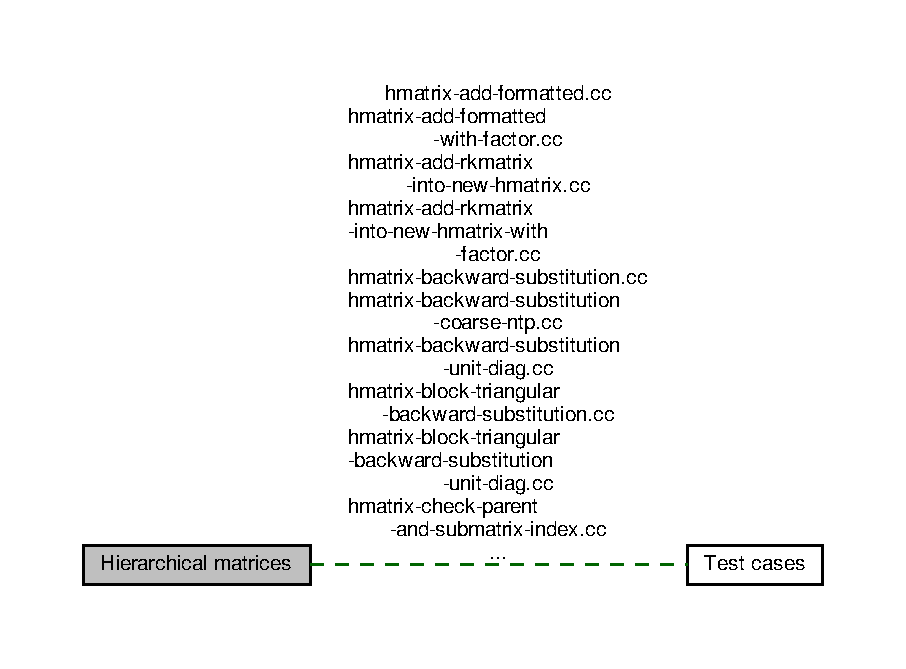
\includegraphics[width=350pt]{group__hierarchical__matrices}
\end{center}
\end{figure}
\subsection*{Files}
\begin{DoxyCompactItemize}
\item 
file \hyperlink{block__cluster_8h}{block\+\_\+cluster.\+h}
\begin{DoxyCompactList}\small\item\em Implementation of the class \hyperlink{classBlockCluster}{Block\+Cluster}. \end{DoxyCompactList}\item 
file \hyperlink{block__cluster__tree_8h}{block\+\_\+cluster\+\_\+tree.\+h}
\begin{DoxyCompactList}\small\item\em Implementation of the class \hyperlink{classBlockClusterTree}{Block\+Cluster\+Tree}. \end{DoxyCompactList}\item 
file \hyperlink{cluster_8h}{cluster.\+h}
\begin{DoxyCompactList}\small\item\em Implementation of the class \hyperlink{classCluster}{Cluster}. \end{DoxyCompactList}\item 
file \hyperlink{hmatrix_8h}{hmatrix.\+h}
\begin{DoxyCompactList}\small\item\em Definition of hierarchical matrix. \end{DoxyCompactList}\item 
file \hyperlink{rkmatrix_8h}{rkmatrix.\+h}
\begin{DoxyCompactList}\small\item\em Definition of rank-\/k matrix. \end{DoxyCompactList}\item 
file \hyperlink{tree_8h}{tree.\+h}
\begin{DoxyCompactList}\small\item\em Implementation of the classes for binary tree node, general tree node and functions for manipulating the trees constructed from these nodes. \end{DoxyCompactList}\item 
file \hyperlink{block-cluster-tree_8cc}{block-\/cluster-\/tree.\+cc}
\begin{DoxyCompactList}\small\item\em This files verifies the admissible block cluster partition. \end{DoxyCompactList}\item 
file \hyperlink{cluster-diameter_8cc}{cluster-\/diameter.\+cc}
\begin{DoxyCompactList}\small\item\em This files verifies the cluster diameter and pair-\/wise distance calculation using a 3x3 grid in a square. \end{DoxyCompactList}\item 
file \hyperlink{cluster-tree-hp_8cc}{cluster-\/tree-\/hp.\+cc}
\begin{DoxyCompactList}\small\item\em Test the construction of a $\mathcal{H}^p$ cluster tree. \end{DoxyCompactList}\item 
file \hyperlink{hmatrix-add-formatted_8cc}{hmatrix-\/add-\/formatted.\+cc}
\begin{DoxyCompactList}\small\item\em Verify formatted addition of two $\mathcal{H}$-\/matrices. \end{DoxyCompactList}\item 
file \hyperlink{hmatrix-add-formatted-with-factor_8cc}{hmatrix-\/add-\/formatted-\/with-\/factor.\+cc}
\begin{DoxyCompactList}\small\item\em Verify formatted addition of two $\mathcal{H}$-\/matrices $C = A + b B$. \end{DoxyCompactList}\item 
file \hyperlink{hmatrix-add-rkmatrix-into-new-hmatrix_8cc}{hmatrix-\/add-\/rkmatrix-\/into-\/new-\/hmatrix.\+cc}
\begin{DoxyCompactList}\small\item\em Verify the addition of a rank-\/k matrix and an $\mathcal{H}$-\/matrix into a new $\mathcal{H}$-\/matrix. \end{DoxyCompactList}\item 
file \hyperlink{hmatrix-add-rkmatrix-into-new-hmatrix-with-factor_8cc}{hmatrix-\/add-\/rkmatrix-\/into-\/new-\/hmatrix-\/with-\/factor.\+cc}
\begin{DoxyCompactList}\small\item\em Verify the addition of a rank-\/k matrix multiplied by a factor and an $\mathcal{H}$-\/matrix into a new $\mathcal{H}$-\/matrix. \end{DoxyCompactList}\item 
file \hyperlink{hmatrix-backward-substitution_8cc}{hmatrix-\/backward-\/substitution.\+cc}
\begin{DoxyCompactList}\small\item\em Verify backward substitution of an upper triangle $\mathcal{H}$-\/matrix. The block cluster tree partition structure is fine non-\/tensor product. \end{DoxyCompactList}\item 
file \hyperlink{hmatrix-backward-substitution-coarse-ntp_8cc}{hmatrix-\/backward-\/substitution-\/coarse-\/ntp.\+cc}
\begin{DoxyCompactList}\small\item\em Verify backward substitution of an upper triangle $\mathcal{H}$-\/matrix. The block cluster tree partition structure is coarse non-\/tensor product. \end{DoxyCompactList}\item 
file \hyperlink{hmatrix-backward-substitution-unit-diag_8cc}{hmatrix-\/backward-\/substitution-\/unit-\/diag.\+cc}
\begin{DoxyCompactList}\small\item\em Verify backward substitution of an unit upper triangle $\mathcal{H}$-\/matrix. The block cluster tree partition structure is fine non-\/tensor product. \end{DoxyCompactList}\item 
file \hyperlink{hmatrix-bct-struct-with-rank_8cc}{hmatrix-\/bct-\/struct-\/with-\/rank.\+cc}
\begin{DoxyCompactList}\small\item\em Visualize the block cluster tree structure of an H-\/matrix with displayed rank. \end{DoxyCompactList}\item 
file \hyperlink{hmatrix-block-triangular-backward-substitution_8cc}{hmatrix-\/block-\/triangular-\/backward-\/substitution.\+cc}
\begin{DoxyCompactList}\small\item\em Verify backward substitution of an upper block triangle $\mathcal{H}$-\/matrix. The block cluster tree partition structure is fine non-\/tensor product. \end{DoxyCompactList}\item 
file \hyperlink{hmatrix-block-triangular-backward-substitution-unit-diag_8cc}{hmatrix-\/block-\/triangular-\/backward-\/substitution-\/unit-\/diag.\+cc}
\begin{DoxyCompactList}\small\item\em Verify backward substitution of an unit upper block triangle $\mathcal{H}$-\/matrix. The block cluster tree partition structure is fine non-\/tensor product. \end{DoxyCompactList}\item 
file \hyperlink{hmatrix-check-parent-and-submatrix-index_8cc}{hmatrix-\/check-\/parent-\/and-\/submatrix-\/index.\+cc}
\begin{DoxyCompactList}\small\item\em Check the {\ttfamily parent} and {\ttfamily submatrix\+\_\+index} member variables of $\mathcal{H}$-\/matrix. \end{DoxyCompactList}\item 
file \hyperlink{hmatrix-cholesky-backward-substitution_8cc}{hmatrix-\/cholesky-\/backward-\/substitution.\+cc}
\begin{DoxyCompactList}\small\item\em Verify backward substitution for the lower triangle $\mathcal{H}$-\/matrix obtained from Cholesky decomposition. The block cluster tree partition structure is fine non-\/tensor product. \end{DoxyCompactList}\item 
file \hyperlink{hmatrix-cholesky-transpose-forward-substitution-matrix-valued_8cc}{hmatrix-\/cholesky-\/transpose-\/forward-\/substitution-\/matrix-\/valued.\+cc}
\begin{DoxyCompactList}\small\item\em Verify matrix-\/valued forward substitution of the transpose of a upper triangular $\mathcal{H}$-\/matrix. \end{DoxyCompactList}\item 
file \hyperlink{hmatrix-coarsening_8cc}{hmatrix-\/coarsening.\+cc}
\begin{DoxyCompactList}\small\item\em Coarsen a H-\/matrix to its subtree. \end{DoxyCompactList}\item 
file \hyperlink{hmatrix-find-diagonal-blocks_8cc}{hmatrix-\/find-\/diagonal-\/blocks.\+cc}
\begin{DoxyCompactList}\small\item\em Find the diagonal blocks related to the current $\mathcal{H}$-\/matrix node. \end{DoxyCompactList}\item 
file \hyperlink{hmatrix-fine-ntp-to-tp_8cc}{hmatrix-\/fine-\/ntp-\/to-\/tp.\+cc}
\begin{DoxyCompactList}\small\item\em Verify the conversion of an $\mathcal{H}$-\/matrix from fine non-\/tensor product structure to tensor product structure. \end{DoxyCompactList}\item 
file \hyperlink{hmatrix-forward-substitution_8cc}{hmatrix-\/forward-\/substitution.\+cc}
\begin{DoxyCompactList}\small\item\em Verify forward substitution of a lower triangle $\mathcal{H}$-\/matrix. The block cluster tree partition structure is fine non-\/tensor product. \end{DoxyCompactList}\item 
file \hyperlink{hmatrix-forward-substitution-coarse-ntp_8cc}{hmatrix-\/forward-\/substitution-\/coarse-\/ntp.\+cc}
\begin{DoxyCompactList}\small\item\em Verify forward substitution of a lower triangle $\mathcal{H}$-\/matrix. The block cluster tree partition structure is coarse non-\/tensor product. \end{DoxyCompactList}\item 
file \hyperlink{hmatrix-forward-substitution-unit-diag_8cc}{hmatrix-\/forward-\/substitution-\/unit-\/diag.\+cc}
\begin{DoxyCompactList}\small\item\em Verify forward substitution of a unit lower triangle $\mathcal{H}$-\/matrix. The block cluster tree partition structure is fine non-\/tensor product. \end{DoxyCompactList}\item 
file \hyperlink{hmatrix-hmatrix-alpha-mmult-level-conserving-all-fine-ntp-member-function-call_8cc}{hmatrix-\/hmatrix-\/alpha-\/mmult-\/level-\/conserving-\/all-\/fine-\/ntp-\/member-\/function-\/call.\+cc}
\begin{DoxyCompactList}\small\item\em Verify the multiplication of two level-\/conserving $\mathcal{H}$-\/matrices with the result scaled by a factor, i.\+e. $M = M + \alpha \cdot M_1 M_2$. Both operands and the result matrices have the fine non-\/tensor product partitions. This version uses the member function call of multiplication. \end{DoxyCompactList}\item 
file \hyperlink{hmatrix-hmatrix-alpha-mTmult-level-conserving-all-fine-ntp-member-function-call_8cc}{hmatrix-\/hmatrix-\/alpha-\/m\+Tmult-\/level-\/conserving-\/all-\/fine-\/ntp-\/member-\/function-\/call.\+cc}
\begin{DoxyCompactList}\small\item\em Verify the multiplication of two level-\/conserving $\mathcal{H}$-\/matrices with the second operand transposed and with the result scaled by a factor, i.\+e. $M = M + \alpha \cdot M_1 M_2$. Both operands and the result matrices have the fine non-\/tensor product partitions. This version uses the member function call of multiplication. \end{DoxyCompactList}\item 
file \hyperlink{hmatrix-hmatrix-mmult-level-conserving-all-fine-ntp_8cc}{hmatrix-\/hmatrix-\/mmult-\/level-\/conserving-\/all-\/fine-\/ntp.\+cc}
\begin{DoxyCompactList}\small\item\em Verify the multiplication of two level-\/conserving $\mathcal{H}$-\/matrices. Both operands and the result matrices have the fine non-\/tensor product partitions. \end{DoxyCompactList}\item 
file \hyperlink{hmatrix-hmatrix-mmult-level-conserving-coarse-coarse-fine-ntp_8cc}{hmatrix-\/hmatrix-\/mmult-\/level-\/conserving-\/coarse-\/coarse-\/fine-\/ntp.\+cc}
\begin{DoxyCompactList}\small\item\em Verify the multiplication of two level-\/conserving $\mathcal{H}$-\/matrices. Both operands have the coarse non-\/tensor product partitions, while the result matrix has the fine non-\/tensor product partitions. \end{DoxyCompactList}\item 
file \hyperlink{hmatrix-hmatrix-mmult-level-conserving-coarse-fine-coarse-ntp_8cc}{hmatrix-\/hmatrix-\/mmult-\/level-\/conserving-\/coarse-\/fine-\/coarse-\/ntp.\+cc}
\begin{DoxyCompactList}\small\item\em Verify the multiplication of two level-\/conserving $\mathcal{H}$-\/matrices. The first operand and the result matrix have the coarse non-\/tensor product partitions, while the second operand has the fine non-\/tensor product partitions. \end{DoxyCompactList}\item 
file \hyperlink{hmatrix-hmatrix-mmult-level-conserving-fine-coarse-fine-ntp_8cc}{hmatrix-\/hmatrix-\/mmult-\/level-\/conserving-\/fine-\/coarse-\/fine-\/ntp.\+cc}
\begin{DoxyCompactList}\small\item\em Verify the multiplication of two level-\/conserving $\mathcal{H}$-\/matrices. The first operand and the result matrix have the fine non-\/tensor product partitions, while the second operand has the coarse non-\/tensor product partitions. \end{DoxyCompactList}\item 
file \hyperlink{hmatrix-hmatrix-mmult-level-conserving-fine-fine-coarse-ntp_8cc}{hmatrix-\/hmatrix-\/mmult-\/level-\/conserving-\/fine-\/fine-\/coarse-\/ntp.\+cc}
\begin{DoxyCompactList}\small\item\em Verify the multiplication of two level-\/conserving $\mathcal{H}$-\/matrices. Both operands have the fine non-\/tensor product partitions, while the result matrix has the coarse non-\/tensor product partitions. \end{DoxyCompactList}\item 
file \hyperlink{hmatrix-hmatrix-mTmult-level-conserving-all-fine-ntp_8cc}{hmatrix-\/hmatrix-\/m\+Tmult-\/level-\/conserving-\/all-\/fine-\/ntp.\+cc}
\begin{DoxyCompactList}\small\item\em Verify the multiplication of two level-\/conserving $\mathcal{H}$-\/matrices with the second operand transposed. Both operands and the result matrices have the fine non-\/tensor product partitions. \end{DoxyCompactList}\item 
file \hyperlink{hmatrix-hmatrix-mTmult-level-conserving-coarse-coarse-fine-ntp_8cc}{hmatrix-\/hmatrix-\/m\+Tmult-\/level-\/conserving-\/coarse-\/coarse-\/fine-\/ntp.\+cc}
\begin{DoxyCompactList}\small\item\em Verify the multiplication of two level-\/conserving $\mathcal{H}$-\/matrices with the second operand transposed. Both operands have the coarse non-\/tensor product partitions, while the result matrix has the fine non-\/tensor product partitions. \end{DoxyCompactList}\item 
file \hyperlink{hmatrix-hmatrix-mTmult-level-conserving-coarse-fine-coarse-ntp_8cc}{hmatrix-\/hmatrix-\/m\+Tmult-\/level-\/conserving-\/coarse-\/fine-\/coarse-\/ntp.\+cc}
\begin{DoxyCompactList}\small\item\em Verify the multiplication of two level-\/conserving $\mathcal{H}$-\/matrices with the second operand transposed. The first operand and the result matrix have the coarse non-\/tensor product partitions, while the second operand has the fine non-\/tensor product partitions. \end{DoxyCompactList}\item 
file \hyperlink{hmatrix-hmatrix-mTmult-level-conserving-fine-coarse-fine-ntp_8cc}{hmatrix-\/hmatrix-\/m\+Tmult-\/level-\/conserving-\/fine-\/coarse-\/fine-\/ntp.\+cc}
\begin{DoxyCompactList}\small\item\em Verify the multiplication of two level-\/conserving $\mathcal{H}$-\/matrices with the second operand transposed. The first operand and the result matrix have the fine non-\/tensor product partitions, while the second operand has the coarse non-\/tensor product partitions. \end{DoxyCompactList}\item 
file \hyperlink{hmatrix-hmatrix-mTmult-level-conserving-fine-fine-coarse-ntp_8cc}{hmatrix-\/hmatrix-\/m\+Tmult-\/level-\/conserving-\/fine-\/fine-\/coarse-\/ntp.\+cc}
\begin{DoxyCompactList}\small\item\em Verify the multiplication of two level-\/conserving $\mathcal{H}$-\/matrices with the second operand transposed. Both operands have the fine non-\/tensor product partitions, while the result matrix has the coarse non-\/tensor product partitions. \end{DoxyCompactList}\item 
file \hyperlink{hmatrix-rkmatrix-conversion_8cc}{hmatrix-\/rkmatrix-\/conversion.\+cc}
\begin{DoxyCompactList}\small\item\em Verify the conversion from an H-\/matrix to a rank-\/k matrix. \end{DoxyCompactList}\item 
file \hyperlink{hmatrix-solve-cholesky_8cc}{hmatrix-\/solve-\/cholesky.\+cc}
\begin{DoxyCompactList}\small\item\em Verify Cholesky factorization of a positive definite and symmetric $\mathcal{H}$-\/matrix and solve this matrix using forward and backward substitution. \end{DoxyCompactList}\item 
file \hyperlink{hmatrix-solve-cholesky-in-situ_8cc}{hmatrix-\/solve-\/cholesky-\/in-\/situ.\+cc}
\begin{DoxyCompactList}\small\item\em Verify in situ Cholesky factorization of a positive definite and symmetric $\mathcal{H}$-\/matrix and solve this matrix using forward and backward substitution. \end{DoxyCompactList}\item 
file \hyperlink{hmatrix-solve-lu_8cc}{hmatrix-\/solve-\/lu.\+cc}
\begin{DoxyCompactList}\small\item\em Verify LU factorization of an $\mathcal{H}$-\/matrix and solve this matrix using forward and backward substitution. \end{DoxyCompactList}\item 
file \hyperlink{hmatrix-solve-lu-in-situ_8cc}{hmatrix-\/solve-\/lu-\/in-\/situ.\+cc}
\begin{DoxyCompactList}\small\item\em Verify LU factorization (in-\/situ) of an $\mathcal{H}$-\/matrix and solve this matrix using forward and backward substitution. \end{DoxyCompactList}\item 
file \hyperlink{hmatrix-transpose-forward-substitution_8cc}{hmatrix-\/transpose-\/forward-\/substitution.\+cc}
\begin{DoxyCompactList}\small\item\em Verify forward substitution of the transpose of an upper triangle $\mathcal{H}$-\/matrix. The block cluster tree partition structure is fine non-\/tensor product. \end{DoxyCompactList}\item 
file \hyperlink{hmatrix-transpose-forward-substitution-matrix-valued_8cc}{hmatrix-\/transpose-\/forward-\/substitution-\/matrix-\/valued.\+cc}
\begin{DoxyCompactList}\small\item\em Verify matrix-\/valued forward substitution of the transpose of a upper triangular $\mathcal{H}$-\/matrix. \end{DoxyCompactList}\item 
file \hyperlink{hmatrix-truncate-to-fixed-rank_8cc}{hmatrix-\/truncate-\/to-\/fixed-\/rank.\+cc}
\begin{DoxyCompactList}\small\item\em Verify the truncation of an \hyperlink{classHMatrix}{H\+Matrix} to an \hyperlink{classRkMatrix}{Rk\+Matrix}. \end{DoxyCompactList}\item 
file \hyperlink{hp-matrix_8cc}{hp-\/matrix.\+cc}
\begin{DoxyCompactList}\small\item\em Test the $H^p$ matrix. \end{DoxyCompactList}\item 
file \hyperlink{rkmatrix-agglomeration_8cc}{rkmatrix-\/agglomeration.\+cc}
\begin{DoxyCompactList}\small\item\em Verify the agglomeration of four rank-\/k submatrices into a larger rank-\/k matrix. \end{DoxyCompactList}\end{DoxyCompactItemize}
\subsection*{Classes}
\begin{DoxyCompactItemize}
\item 
class \hyperlink{classBlockCluster}{Block\+Cluster$<$ spacedim, Number $>$}
\begin{DoxyCompactList}\small\item\em Class for block cluster. \end{DoxyCompactList}\item 
class \hyperlink{classBlockClusterTree}{Block\+Cluster\+Tree$<$ spacedim, Number $>$}
\begin{DoxyCompactList}\small\item\em Class for block cluster tree. \end{DoxyCompactList}\item 
class \hyperlink{classBinaryTreeNode}{Binary\+Tree\+Node$<$ T $>$}
\begin{DoxyCompactList}\small\item\em Class for binary tree node. \end{DoxyCompactList}\end{DoxyCompactItemize}
\begin{DoxyCompactItemize}
\item 
{\footnotesize template$<$int dim, int spacedim, typename Number  = double$>$ }\\void \hyperlink{group__hierarchical__matrices_gaeba0b2d80f64d0bb5c1ad86ac31bbcda}{map\+\_\+dofs\+\_\+to\+\_\+average\+\_\+cell\+\_\+size} (const Do\+F\+Handler$<$ dim, spacedim $>$ \&dof\+\_\+handler, std\+::vector$<$ Number $>$ \&dof\+\_\+average\+\_\+cell\+\_\+size)
\item 
{\footnotesize template$<$typename Do\+F\+Handler\+Type , typename Number  = double$>$ }\\void \hyperlink{group__hierarchical__matrices_ga1eee708f9eb5b9e9a2d8031c60c5d315}{map\+\_\+dofs\+\_\+to\+\_\+max\+\_\+cell\+\_\+size} (const Do\+F\+Handler\+Type \&dof\+\_\+handler, std\+::vector$<$ Number $>$ \&dof\+\_\+max\+\_\+cell\+\_\+size)
\item 
{\footnotesize template$<$typename Do\+F\+Handler\+Type , typename Number  = double$>$ }\\void \hyperlink{group__hierarchical__matrices_ga0a1c7de8480c4e9b4a002818f8c19b52}{map\+\_\+dofs\+\_\+to\+\_\+min\+\_\+cell\+\_\+size} (const Do\+F\+Handler\+Type \&dof\+\_\+handler, std\+::vector$<$ Number $>$ \&dof\+\_\+min\+\_\+cell\+\_\+size)
\item 
{\footnotesize template$<$int spacedim, typename Number $>$ }\\std\+::ostream \& \hyperlink{group__hierarchical__matrices_ga79f6d9af30209ae20bdf81906360664a}{operator$<$$<$} (std\+::ostream \&out, const \hyperlink{classCluster}{Cluster}$<$ spacedim, Number $>$ \&cluster)
\item 
{\footnotesize template$<$int spacedim, typename Number  = double$>$ }\\Number \hyperlink{group__hierarchical__matrices_gab6b0a51fb1b117f29902d220df72420a}{calc\+\_\+cluster\+\_\+distance} (const \hyperlink{classCluster}{Cluster}$<$ spacedim, Number $>$ \&cluster1, const \hyperlink{classCluster}{Cluster}$<$ spacedim, Number $>$ \&cluster2, const std\+::vector$<$ Point$<$ spacedim, Number $>$$>$ \&all\+\_\+support\+\_\+points)
\item 
{\footnotesize template$<$int spacedim, typename Number  = double$>$ }\\Number \hyperlink{group__hierarchical__matrices_ga76ef8db7b1a8500eac8d807bf104cacb}{calc\+\_\+cluster\+\_\+distance} (const \hyperlink{classCluster}{Cluster}$<$ spacedim, Number $>$ \&cluster1, const \hyperlink{classCluster}{Cluster}$<$ spacedim, Number $>$ \&cluster2, const std\+::vector$<$ Point$<$ spacedim, Number $>$$>$ \&all\+\_\+support\+\_\+points, const std\+::vector$<$ Number $>$ \&cell\+\_\+size\+\_\+at\+\_\+dofs)
\item 
\mbox{\Hypertarget{group__hierarchical__matrices_gacb7726d12648a539547a7520c6b699e9}\label{group__hierarchical__matrices_gacb7726d12648a539547a7520c6b699e9}} 
{\footnotesize template$<$int spacedim, typename Number $>$ }\\bool {\bfseries operator==} (const \hyperlink{classCluster}{Cluster}$<$ spacedim, Number $>$ \&cluster1, const \hyperlink{classCluster}{Cluster}$<$ spacedim, Number $>$ \&cluster2)
\end{DoxyCompactItemize}


\subsection{Detailed Description}
Implementation of hierarchical matrix data structure and algebraic operations. 



\subsection{Function Documentation}
\mbox{\Hypertarget{group__hierarchical__matrices_gab6b0a51fb1b117f29902d220df72420a}\label{group__hierarchical__matrices_gab6b0a51fb1b117f29902d220df72420a}} 
\index{Hierarchical matrices@{Hierarchical matrices}!calc\+\_\+cluster\+\_\+distance@{calc\+\_\+cluster\+\_\+distance}}
\index{calc\+\_\+cluster\+\_\+distance@{calc\+\_\+cluster\+\_\+distance}!Hierarchical matrices@{Hierarchical matrices}}
\subsubsection{\texorpdfstring{calc\+\_\+cluster\+\_\+distance()}{calc\_cluster\_distance()}\hspace{0.1cm}{\footnotesize\ttfamily [1/2]}}
{\footnotesize\ttfamily template$<$int spacedim, typename Number  = double$>$ \\
Number calc\+\_\+cluster\+\_\+distance (\begin{DoxyParamCaption}\item[{const \hyperlink{classCluster}{Cluster}$<$ spacedim, Number $>$ \&}]{cluster1,  }\item[{const \hyperlink{classCluster}{Cluster}$<$ spacedim, Number $>$ \&}]{cluster2,  }\item[{const std\+::vector$<$ Point$<$ spacedim, Number $>$$>$ \&}]{all\+\_\+support\+\_\+points }\end{DoxyParamCaption})}

Calculate the minimum distance between two clusters. This calculation has no mesh size correction.

The calculation is based on measuring the distance between each pair of support points contained in the clusters, which prevents the distance calculation between two support sets. 
\begin{DoxyParams}{Parameters}
{\em cluster1} & \\
\hline
{\em cluster2} & \\
\hline
{\em all\+\_\+support\+\_\+points} & A list of support point coordinates which are ordered by DoF indices. \\
\hline
\end{DoxyParams}
\begin{DoxyReturn}{Returns}

\end{DoxyReturn}


References Cluster$<$ spacedim, Number $>$\+::get\+\_\+index\+\_\+set().

\mbox{\Hypertarget{group__hierarchical__matrices_ga76ef8db7b1a8500eac8d807bf104cacb}\label{group__hierarchical__matrices_ga76ef8db7b1a8500eac8d807bf104cacb}} 
\index{Hierarchical matrices@{Hierarchical matrices}!calc\+\_\+cluster\+\_\+distance@{calc\+\_\+cluster\+\_\+distance}}
\index{calc\+\_\+cluster\+\_\+distance@{calc\+\_\+cluster\+\_\+distance}!Hierarchical matrices@{Hierarchical matrices}}
\subsubsection{\texorpdfstring{calc\+\_\+cluster\+\_\+distance()}{calc\_cluster\_distance()}\hspace{0.1cm}{\footnotesize\ttfamily [2/2]}}
{\footnotesize\ttfamily template$<$int spacedim, typename Number  = double$>$ \\
Number calc\+\_\+cluster\+\_\+distance (\begin{DoxyParamCaption}\item[{const \hyperlink{classCluster}{Cluster}$<$ spacedim, Number $>$ \&}]{cluster1,  }\item[{const \hyperlink{classCluster}{Cluster}$<$ spacedim, Number $>$ \&}]{cluster2,  }\item[{const std\+::vector$<$ Point$<$ spacedim, Number $>$$>$ \&}]{all\+\_\+support\+\_\+points,  }\item[{const std\+::vector$<$ Number $>$ \&}]{cell\+\_\+size\+\_\+at\+\_\+dofs }\end{DoxyParamCaption})}

Calculate the minimum distance between two clusters. This calculation has the mesh size correction.

The calculation is based on measuring the distance between each pair of support points contained in the clusters, which prevents the distance calculation between two support sets. 
\begin{DoxyParams}{Parameters}
{\em cluster1} & \\
\hline
{\em cluster2} & \\
\hline
{\em all\+\_\+support\+\_\+points} & A list of support point coordinates which are ordered by DoF indices. \\
\hline
{\em cell\+\_\+size\+\_\+at\+\_\+dofs} & The list of estimated cell size values at DoF support points. \\
\hline
\end{DoxyParams}
\begin{DoxyReturn}{Returns}

\end{DoxyReturn}
Calculate the uncorrected cluster distance.

Get the maximum diameter of the support sets for different Do\+Fs, which is 2 times of the cell size associated with the corresponding DoF.

Ensure the positivity of the returned cluster distance.

References Cluster$<$ spacedim, Number $>$\+::get\+\_\+index\+\_\+set().

\mbox{\Hypertarget{group__hierarchical__matrices_gaeba0b2d80f64d0bb5c1ad86ac31bbcda}\label{group__hierarchical__matrices_gaeba0b2d80f64d0bb5c1ad86ac31bbcda}} 
\index{Hierarchical matrices@{Hierarchical matrices}!map\+\_\+dofs\+\_\+to\+\_\+average\+\_\+cell\+\_\+size@{map\+\_\+dofs\+\_\+to\+\_\+average\+\_\+cell\+\_\+size}}
\index{map\+\_\+dofs\+\_\+to\+\_\+average\+\_\+cell\+\_\+size@{map\+\_\+dofs\+\_\+to\+\_\+average\+\_\+cell\+\_\+size}!Hierarchical matrices@{Hierarchical matrices}}
\subsubsection{\texorpdfstring{map\+\_\+dofs\+\_\+to\+\_\+average\+\_\+cell\+\_\+size()}{map\_dofs\_to\_average\_cell\_size()}}
{\footnotesize\ttfamily template$<$int dim, int spacedim, typename Number  = double$>$ \\
void map\+\_\+dofs\+\_\+to\+\_\+average\+\_\+cell\+\_\+size (\begin{DoxyParamCaption}\item[{const Do\+F\+Handler$<$ dim, spacedim $>$ \&}]{dof\+\_\+handler,  }\item[{std\+::vector$<$ Number $>$ \&}]{dof\+\_\+average\+\_\+cell\+\_\+size }\end{DoxyParamCaption})}

Calculate the average cell sizes associated with those Do\+Fs handled by the given DoF handler object.

The value doubled is used as an estimate for the diameter of the support set of each DoF.


\begin{DoxyParams}{Parameters}
{\em dof\+\_\+average\+\_\+cell\+\_\+size} & The returned list of average cell sizes. The memory for this vector should be preallocated and initialized to zero before calling this function. \\
\hline
\end{DoxyParams}
Create the vector which stores the number of cells that share a common DoF for each DoF.

Get the diameter of the current cell.

Get DoF indices local to this cell.

Referenced by main().

\mbox{\Hypertarget{group__hierarchical__matrices_ga1eee708f9eb5b9e9a2d8031c60c5d315}\label{group__hierarchical__matrices_ga1eee708f9eb5b9e9a2d8031c60c5d315}} 
\index{Hierarchical matrices@{Hierarchical matrices}!map\+\_\+dofs\+\_\+to\+\_\+max\+\_\+cell\+\_\+size@{map\+\_\+dofs\+\_\+to\+\_\+max\+\_\+cell\+\_\+size}}
\index{map\+\_\+dofs\+\_\+to\+\_\+max\+\_\+cell\+\_\+size@{map\+\_\+dofs\+\_\+to\+\_\+max\+\_\+cell\+\_\+size}!Hierarchical matrices@{Hierarchical matrices}}
\subsubsection{\texorpdfstring{map\+\_\+dofs\+\_\+to\+\_\+max\+\_\+cell\+\_\+size()}{map\_dofs\_to\_max\_cell\_size()}}
{\footnotesize\ttfamily template$<$typename Do\+F\+Handler\+Type , typename Number  = double$>$ \\
void map\+\_\+dofs\+\_\+to\+\_\+max\+\_\+cell\+\_\+size (\begin{DoxyParamCaption}\item[{const Do\+F\+Handler\+Type \&}]{dof\+\_\+handler,  }\item[{std\+::vector$<$ Number $>$ \&}]{dof\+\_\+max\+\_\+cell\+\_\+size }\end{DoxyParamCaption})}

Calculate the maximum cell sizes associated with those Do\+Fs handled by the given DoF handler object.

The value doubled is used as an estimate for the diameter of the support set of each DoF.


\begin{DoxyParams}{Parameters}
{\em dof\+\_\+max\+\_\+cell\+\_\+size} & The returned list of maximum cell sizes. The memory for this vector should be preallocated and initialized to zero before calling this function. \\
\hline
\end{DoxyParams}
Get the diameter of the current cell.

Get DoF indices local to this cell.

Referenced by main().

\mbox{\Hypertarget{group__hierarchical__matrices_ga0a1c7de8480c4e9b4a002818f8c19b52}\label{group__hierarchical__matrices_ga0a1c7de8480c4e9b4a002818f8c19b52}} 
\index{Hierarchical matrices@{Hierarchical matrices}!map\+\_\+dofs\+\_\+to\+\_\+min\+\_\+cell\+\_\+size@{map\+\_\+dofs\+\_\+to\+\_\+min\+\_\+cell\+\_\+size}}
\index{map\+\_\+dofs\+\_\+to\+\_\+min\+\_\+cell\+\_\+size@{map\+\_\+dofs\+\_\+to\+\_\+min\+\_\+cell\+\_\+size}!Hierarchical matrices@{Hierarchical matrices}}
\subsubsection{\texorpdfstring{map\+\_\+dofs\+\_\+to\+\_\+min\+\_\+cell\+\_\+size()}{map\_dofs\_to\_min\_cell\_size()}}
{\footnotesize\ttfamily template$<$typename Do\+F\+Handler\+Type , typename Number  = double$>$ \\
void map\+\_\+dofs\+\_\+to\+\_\+min\+\_\+cell\+\_\+size (\begin{DoxyParamCaption}\item[{const Do\+F\+Handler\+Type \&}]{dof\+\_\+handler,  }\item[{std\+::vector$<$ Number $>$ \&}]{dof\+\_\+min\+\_\+cell\+\_\+size }\end{DoxyParamCaption})}

Calculate the minimum cell sizes associated with those Do\+Fs handled by the given DoF handler object.

The value doubled is used as an estimate for the diameter of the support set of each DoF.


\begin{DoxyParams}{Parameters}
{\em dof\+\_\+min\+\_\+cell\+\_\+size} & The returned list of average cell sizes. The memory for this vector should be preallocated and initialized to zero before calling this function. \\
\hline
\end{DoxyParams}
Get the diameter of the current cell.

Get DoF indices local to this cell.

Referenced by main().

\mbox{\Hypertarget{group__hierarchical__matrices_ga79f6d9af30209ae20bdf81906360664a}\label{group__hierarchical__matrices_ga79f6d9af30209ae20bdf81906360664a}} 
\index{Hierarchical matrices@{Hierarchical matrices}!operator$<$$<$@{operator$<$$<$}}
\index{operator$<$$<$@{operator$<$$<$}!Hierarchical matrices@{Hierarchical matrices}}
\subsubsection{\texorpdfstring{operator$<$$<$()}{operator<<()}}
{\footnotesize\ttfamily template$<$int spacedim, typename Number $>$ \\
std\+::ostream\& operator$<$$<$ (\begin{DoxyParamCaption}\item[{std\+::ostream \&}]{out,  }\item[{const \hyperlink{classCluster}{Cluster}$<$ spacedim, Number $>$ \&}]{cluster }\end{DoxyParamCaption})}

Print out the cluster data. 
\begin{DoxyParams}{Parameters}
{\em out} & \\
\hline
{\em cluster} & \\
\hline
\end{DoxyParams}
\begin{DoxyReturn}{Returns}

\end{DoxyReturn}

\hypertarget{group__sauter__quadrature}{}\section{Sauter quadrature}
\label{group__sauter__quadrature}\index{Sauter quadrature@{Sauter quadrature}}


Implementation of Stefan Sauter\textquotesingle{}s method about 4D numerical quadrature which aims to handle singularity.  


\subsection*{Files}
\begin{DoxyCompactItemize}
\item 
file \hyperlink{laplace__bem_8h}{laplace\+\_\+bem.\+h}
\begin{DoxyCompactList}\small\item\em Implementation of B\+EM involving kernel functions and singular numerical quadratures. \end{DoxyCompactList}\end{DoxyCompactItemize}


\subsection{Detailed Description}
Implementation of Stefan Sauter\textquotesingle{}s method about 4D numerical quadrature which aims to handle singularity. 


\hypertarget{group__toolbox}{}\section{Toolbox}
\label{group__toolbox}\index{Toolbox@{Toolbox}}


This is my toolbox for assisting program debugging, function verification and information visualization.  


\subsection*{Files}
\begin{DoxyCompactItemize}
\item 
file \hyperlink{debug__tools_8h}{debug\+\_\+tools.\+h}
\begin{DoxyCompactList}\small\item\em This file includes a bunch of helper functions for printing out and visualizing information about grid, Do\+Fs, map, etc. \end{DoxyCompactList}\end{DoxyCompactItemize}


\subsection{Detailed Description}
This is my toolbox for assisting program debugging, function verification and information visualization. 


\hypertarget{group__linalg}{}\section{Linear algebra}
\label{group__linalg}\index{Linear algebra@{Linear algebra}}


Linear algebra computation.  


Collaboration diagram for Linear algebra\+:\nopagebreak
\begin{figure}[H]
\begin{center}
\leavevmode
\includegraphics[width=350pt]{group__linalg}
\end{center}
\end{figure}
\subsection*{Files}
\begin{DoxyCompactItemize}
\item 
file \hyperlink{lapack__helpers_8h}{lapack\+\_\+helpers.\+h}
\begin{DoxyCompactList}\small\item\em Exposes L\+A\+P\+A\+CK helper functions defined in lapack\+\_\+full\+\_\+matrix.\+cc and define new ones by following them as examples. \end{DoxyCompactList}\item 
file \hyperlink{lapack-matrix-agglomeration_8cc}{lapack-\/matrix-\/agglomeration.\+cc}
\begin{DoxyCompactList}\small\item\em Verify the agglomeration of four full submatrices into a larger full matrix. \end{DoxyCompactList}\item 
file \hyperlink{lapack-matrix-backward-substitution_8cc}{lapack-\/matrix-\/backward-\/substitution.\+cc}
\begin{DoxyCompactList}\small\item\em Verify backward substitution of an upper triangle matrix. \end{DoxyCompactList}\item 
file \hyperlink{delete-rows-and-columns_8cc}{delete-\/rows-\/and-\/columns.\+cc}
\begin{DoxyCompactList}\small\item\em Test deleting rows and columns as well as keeping the first {\ttfamily n} rows or columns from a \hyperlink{classLAPACKFullMatrixExt}{L\+A\+P\+A\+C\+K\+Full\+Matrix\+Ext}. . \end{DoxyCompactList}\item 
file \hyperlink{lapack-matrix-fill_8cc}{lapack-\/matrix-\/fill.\+cc}
\begin{DoxyCompactList}\small\item\em Verify filling a \hyperlink{classLAPACKFullMatrixExt}{L\+A\+P\+A\+C\+K\+Full\+Matrix\+Ext} from a source matrix. \end{DoxyCompactList}\item 
file \hyperlink{lapack-matrix-forward-substitution_8cc}{lapack-\/matrix-\/forward-\/substitution.\+cc}
\begin{DoxyCompactList}\small\item\em Verify forward substitution of a unit lower triangle matrix. \end{DoxyCompactList}\item 
file \hyperlink{hstack-vstack_8cc}{hstack-\/vstack.\+cc}
\begin{DoxyCompactList}\small\item\em Verify horizontal and vertical stacking of two \hyperlink{classLAPACKFullMatrixExt}{L\+A\+P\+A\+C\+K\+Full\+Matrix\+Ext} objects. \end{DoxyCompactList}\item 
file \hyperlink{lapack-matrix-read-from-mat_8cc}{lapack-\/matrix-\/read-\/from-\/mat.\+cc}
\begin{DoxyCompactList}\small\item\em Verify reading a matrix from a file saved from Octave in text format, i.\+e. saved with the option {\ttfamily -\/text}. \end{DoxyCompactList}\item 
file \hyperlink{lapack-matrix-scale-matrix_8cc}{lapack-\/matrix-\/scale-\/matrix.\+cc}
\begin{DoxyCompactList}\small\item\em Verify the scale of a whole full matrix. \end{DoxyCompactList}\item 
file \hyperlink{scale-rows-and-columns_8cc}{scale-\/rows-\/and-\/columns.\+cc}
\begin{DoxyCompactList}\small\item\em Test scaling rows and columns of a \hyperlink{classLAPACKFullMatrixExt}{L\+A\+P\+A\+C\+K\+Full\+Matrix\+Ext}, which is actually left and right multiplication with a diagonal matrix. \end{DoxyCompactList}\item 
file \hyperlink{lapack-matrix-solve-by-cholesky_8cc}{lapack-\/matrix-\/solve-\/by-\/cholesky.\+cc}
\begin{DoxyCompactList}\small\item\em Verify solving a full matrix using Cholesky decomposition. \end{DoxyCompactList}\item 
file \hyperlink{lapack-matrix-solve-by-lu_8cc}{lapack-\/matrix-\/solve-\/by-\/lu.\+cc}
\begin{DoxyCompactList}\small\item\em Verify solving a full matrix using LU decomposition. \end{DoxyCompactList}\item 
file \hyperlink{svd_8cc}{svd.\+cc}
\begin{DoxyCompactList}\small\item\em Test singular value decomposition (S\+VD) and reduced S\+VD. \end{DoxyCompactList}\item 
file \hyperlink{svd-degenerate-cases_8cc}{svd-\/degenerate-\/cases.\+cc}
\begin{DoxyCompactList}\small\item\em Test S\+VD and R\+S\+VD for degenerate cases, such as the matrix is a scalar, row vector or column vector. \end{DoxyCompactList}\item 
file \hyperlink{transpose_8cc}{transpose.\+cc}
\begin{DoxyCompactList}\small\item\em Test in-\/place transpose of a \hyperlink{classLAPACKFullMatrixExt}{L\+A\+P\+A\+C\+K\+Full\+Matrix\+Ext}. \end{DoxyCompactList}\item 
file \hyperlink{rkmatrix_8cc}{rkmatrix.\+cc}
\begin{DoxyCompactList}\small\item\em Test \hyperlink{classRkMatrix}{Rk\+Matrix} class. \end{DoxyCompactList}\item 
file \hyperlink{rkmatrix-add-formatted_8cc}{rkmatrix-\/add-\/formatted.\+cc}
\begin{DoxyCompactList}\small\item\em Verify the formatted addition of two rank-\/k matrices. \end{DoxyCompactList}\item 
file \hyperlink{rkmatrix-add-formatted-using-qr_8cc}{rkmatrix-\/add-\/formatted-\/using-\/qr.\+cc}
\begin{DoxyCompactList}\small\item\em Verify the formatted addition of two rank-\/k matrices by using the QR decomposition. This requires that the component matrices of rank-\/k matrices should be wide matrix, i.\+e. having more rows than columns. \end{DoxyCompactList}\item 
file \hyperlink{rkmatrix-add-formatted-with-factor_8cc}{rkmatrix-\/add-\/formatted-\/with-\/factor.\+cc}
\begin{DoxyCompactList}\small\item\em Verify the formatted addition of two rank-\/k matrices $C = A + b B$. \end{DoxyCompactList}\end{DoxyCompactItemize}


\subsection{Detailed Description}
Linear algebra computation. 


\hypertarget{group__programming__tech}{}\section{Programming techniques}
\label{group__programming__tech}\index{Programming techniques@{Programming techniques}}


Programming techniques for C++ and software engineering.  


Programming techniques for C++ and software engineering. 


\hypertarget{group__testers}{}\section{Test cases}
\label{group__testers}\index{Test cases@{Test cases}}


Test cases for verifying code design and algorithms.  


Collaboration diagram for Test cases\+:\nopagebreak
\begin{figure}[H]
\begin{center}
\leavevmode
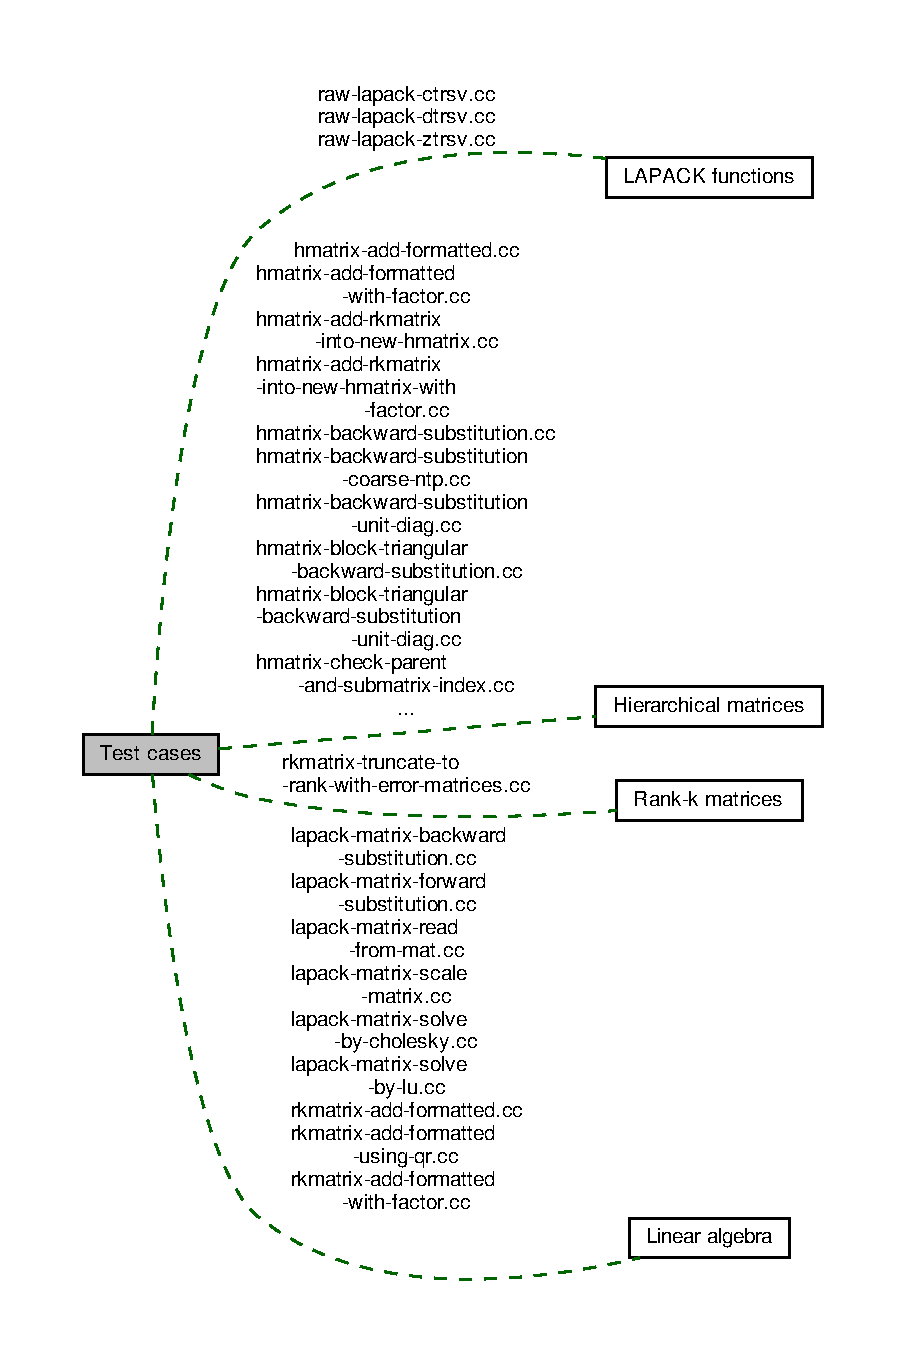
\includegraphics[width=350pt]{group__testers}
\end{center}
\end{figure}
\subsection*{Files}
\begin{DoxyCompactItemize}
\item 
file \hyperlink{bct-extend-to-finer-partition_8cc}{bct-\/extend-\/to-\/finer-\/partition.\+cc}
\begin{DoxyCompactList}\small\item\em Verify extend a block cluster tree to a given finer partition. \end{DoxyCompactList}\item 
file \hyperlink{bct-overloaded-assignment_8cc}{bct-\/overloaded-\/assignment.\+cc}
\begin{DoxyCompactList}\small\item\em Verify the deep and shallow overloaded assignment operators for {\ttfamily \hyperlink{classBlockClusterTree}{Block\+Cluster\+Tree}}. \end{DoxyCompactList}\item 
file \hyperlink{fullmatrix-hmatrix-mmult_8cc}{fullmatrix-\/hmatrix-\/mmult.\+cc}
\begin{DoxyCompactList}\small\item\em Verify the full matrix/\+H-\/matrix multiplication. \end{DoxyCompactList}\item 
file \hyperlink{hmatrix-coarsening_8cc}{hmatrix-\/coarsening.\+cc}
\begin{DoxyCompactList}\small\item\em Coarsen a H-\/matrix to its subtree. \end{DoxyCompactList}\item 
file \hyperlink{hmatrix-deep-copy-constructor_8cc}{hmatrix-\/deep-\/copy-\/constructor.\+cc}
\begin{DoxyCompactList}\small\item\em Verify the deep copy constructor of $\mathcal{H}$-\/matrix. \end{DoxyCompactList}\item 
file \hyperlink{hmatrix-fine-ntp-to-tp_8cc}{hmatrix-\/fine-\/ntp-\/to-\/tp.\+cc}
\begin{DoxyCompactList}\small\item\em Verify the conversion of an $\mathcal{H}$-\/matrix from fine non-\/tensor product structure to tensor product structure. \end{DoxyCompactList}\item 
file \hyperlink{hmatrix-fullmatrix-mmult_8cc}{hmatrix-\/fullmatrix-\/mmult.\+cc}
\begin{DoxyCompactList}\small\item\em Verify the H-\/matrix/full matrix multiplication. \end{DoxyCompactList}\item 
file \hyperlink{hmatrix-hmatrix-mmult-all-coarse-ntp_8cc}{hmatrix-\/hmatrix-\/mmult-\/all-\/coarse-\/ntp.\+cc}
\begin{DoxyCompactList}\small\item\em Verify the multiplication of two $\mathcal{H}$-\/matrices. Both operands and the result matrices have the coarse non-\/tensor product partitions. \end{DoxyCompactList}\item 
file \hyperlink{hmatrix-hmatrix-mmult-all-fine-ntp_8cc}{hmatrix-\/hmatrix-\/mmult-\/all-\/fine-\/ntp.\+cc}
\begin{DoxyCompactList}\small\item\em Verify the multiplication of two $\mathcal{H}$-\/matrices. Both operands and the result matrices have the fine non-\/tensor product partitions. \end{DoxyCompactList}\item 
file \hyperlink{hmatrix-hmatrix-mmult-all-fine-ntp-with-adding_8cc}{hmatrix-\/hmatrix-\/mmult-\/all-\/fine-\/ntp-\/with-\/adding.\+cc}
\begin{DoxyCompactList}\small\item\em Verify the multiplication of two $\mathcal{H}$-\/matrices. Both operands and the result matrices have the fine non-\/tensor product partitions. The calculation results will be added to the first operand. \end{DoxyCompactList}\item 
file \hyperlink{hmatrix-hmatrix-mmult-coarse-coarse-fine-ntp_8cc}{hmatrix-\/hmatrix-\/mmult-\/coarse-\/coarse-\/fine-\/ntp.\+cc}
\begin{DoxyCompactList}\small\item\em Verify the multiplication of two $\mathcal{H}$-\/matrices, where M1, M2 and M have coarse-\/coarse-\/fine non-\/tensor product partitions. \end{DoxyCompactList}\item 
file \hyperlink{hmatrix-hmatrix-mmult-coarse-fine-coarse-ntp_8cc}{hmatrix-\/hmatrix-\/mmult-\/coarse-\/fine-\/coarse-\/ntp.\+cc}
\begin{DoxyCompactList}\small\item\em Verify the multiplication of two $\mathcal{H}$-\/matrices, where M1, M2 and M have coarse-\/fine-\/coarse non-\/tensor product partitions. \end{DoxyCompactList}\item 
file \hyperlink{hmatrix-hmatrix-mmult-fine-coarse-fine-ntp_8cc}{hmatrix-\/hmatrix-\/mmult-\/fine-\/coarse-\/fine-\/ntp.\+cc}
\begin{DoxyCompactList}\small\item\em Verify the multiplication of two $\mathcal{H}$-\/matrices, where M1, M2 and M have fine-\/coarse-\/fine non-\/tensor product partitions. \end{DoxyCompactList}\item 
file \hyperlink{hmatrix-hmatrix-mmult-fine-fine-coarse-ntp_8cc}{hmatrix-\/hmatrix-\/mmult-\/fine-\/fine-\/coarse-\/ntp.\+cc}
\begin{DoxyCompactList}\small\item\em Verify the multiplication of two $\mathcal{H}$-\/matrices, where M1, M2 and M have fine-\/fine-\/coarse non-\/tensor product partitions. \end{DoxyCompactList}\item 
file \hyperlink{hmatrix-overloaded-deep-assignment_8cc}{hmatrix-\/overloaded-\/deep-\/assignment.\+cc}
\begin{DoxyCompactList}\small\item\em Verify the overloaded deep assignment operator of $\mathcal{H}$-\/matrix. \end{DoxyCompactList}\item 
file \hyperlink{hmatrix-overloaded-shallow-assignment_8cc}{hmatrix-\/overloaded-\/shallow-\/assignment.\+cc}
\begin{DoxyCompactList}\small\item\em Verify the overloaded shallow assignment operator of $\mathcal{H}$-\/matrix. \end{DoxyCompactList}\item 
file \hyperlink{hmatrix-refinement_8cc}{hmatrix-\/refinement.\+cc}
\begin{DoxyCompactList}\small\item\em Verify the refinement of an $\mathcal{H}$-\/matrix hierarchy with respect to its extended block cluster tree. \end{DoxyCompactList}\item 
file \hyperlink{hmatrix-rkmatrix-conversion_8cc}{hmatrix-\/rkmatrix-\/conversion.\+cc}
\begin{DoxyCompactList}\small\item\em Verify the conversion from an H-\/matrix to a rank-\/k matrix. \end{DoxyCompactList}\item 
file \hyperlink{hmatrix-rkmatrix-mmult_8cc}{hmatrix-\/rkmatrix-\/mmult.\+cc}
\begin{DoxyCompactList}\small\item\em Verify the H-\/matrix/rank-\/k matrix multiplication. \end{DoxyCompactList}\item 
file \hyperlink{hmatrix-shallow-copy-constructor_8cc}{hmatrix-\/shallow-\/copy-\/constructor.\+cc}
\begin{DoxyCompactList}\small\item\em Verify the deep copy constructor of $\mathcal{H}$-\/matrix. \end{DoxyCompactList}\item 
file \hyperlink{hmatrix-truncate-to-fixed-rank_8cc}{hmatrix-\/truncate-\/to-\/fixed-\/rank.\+cc}
\begin{DoxyCompactList}\small\item\em Verify the truncation of an \hyperlink{classHMatrix}{H\+Matrix} to an \hyperlink{classRkMatrix}{Rk\+Matrix}. \end{DoxyCompactList}\item 
file \hyperlink{lapack-matrix-agglomeration-interwoven-indices_8cc}{lapack-\/matrix-\/agglomeration-\/interwoven-\/indices.\+cc}
\begin{DoxyCompactList}\small\item\em Verify the agglomeration of four full submatrices into a larger full matrix when the index sets of several child clusters are interwoven together into the index set of the parent cluster. \end{DoxyCompactList}\item 
file \hyperlink{lapack-matrix-agglomeration-of-two-submatrices_8cc}{lapack-\/matrix-\/agglomeration-\/of-\/two-\/submatrices.\+cc}
\begin{DoxyCompactList}\small\item\em Verify the agglomeration of two full submatrices which have been obtained from horizontal or vertical splitting. \end{DoxyCompactList}\item 
file \hyperlink{lapack-matrix-agglomeration-of-two-submatrices-interwoven-indices_8cc}{lapack-\/matrix-\/agglomeration-\/of-\/two-\/submatrices-\/interwoven-\/indices.\+cc}
\begin{DoxyCompactList}\small\item\em Verify the agglomeration of two full submatrices which have been obtained from horizontal or vertical splitting. The index sets of several child clusters are interwoven together into the index set of the parent cluster. \end{DoxyCompactList}\item 
file \hyperlink{lapack-matrix-inverse_8cc}{lapack-\/matrix-\/inverse.\+cc}
\begin{DoxyCompactList}\small\item\em Verify matrix inverse computed by Gauss elimination, which is compared with the standard function in deal.\+ii. \end{DoxyCompactList}\item 
file \hyperlink{lapack-matrix-mmult_8cc}{lapack-\/matrix-\/mmult.\+cc}
\begin{DoxyCompactList}\small\item\em Verify the multiplication of two {\ttfamily \hyperlink{classLAPACKFullMatrixExt}{L\+A\+P\+A\+C\+K\+Full\+Matrix\+Ext}}. \end{DoxyCompactList}\item 
file \hyperlink{rkmatrix-agglomeration-interwoven-indices_8cc}{rkmatrix-\/agglomeration-\/interwoven-\/indices.\+cc}
\begin{DoxyCompactList}\small\item\em Verify the agglomeration of four rank-\/k submatrices into a larger rank-\/k matrix when the index sets of several child clusters are interwoven together into the index set of the parent cluster. \end{DoxyCompactList}\item 
file \hyperlink{rkmatrix-agglomeration-of-two-submatrices_8cc}{rkmatrix-\/agglomeration-\/of-\/two-\/submatrices.\+cc}
\begin{DoxyCompactList}\small\item\em Verify the agglomeration of two rank-\/k submatrices which have been obtained from horizontal or vertical splitting. \end{DoxyCompactList}\item 
file \hyperlink{rkmatrix-agglomeration-of-two-submatrices-interwoven-indices_8cc}{rkmatrix-\/agglomeration-\/of-\/two-\/submatrices-\/interwoven-\/indices.\+cc}
\begin{DoxyCompactList}\small\item\em Verify the agglomeration of two rank-\/k submatrices which have been obtained from horizontal or vertical splitting. The index sets of several child clusters are interwoven together into the index set of the parent cluster. \end{DoxyCompactList}\item 
file \hyperlink{rkmatrix-hmatrix-mmult_8cc}{rkmatrix-\/hmatrix-\/mmult.\+cc}
\begin{DoxyCompactList}\small\item\em Verify the rank-\/k/\+H-\/matrix matrix multiplication. \end{DoxyCompactList}\end{DoxyCompactItemize}


\subsection{Detailed Description}
Test cases for verifying code design and algorithms. 


\chapter{Class Documentation}
\hypertarget{classLaplaceBEM_1_1LaplaceKernel_1_1AdjointDoubleLayerKernel}{}\section{Laplace\+B\+EM\+:\+:Laplace\+Kernel\+:\+:Adjoint\+Double\+Layer\+Kernel$<$ dim, Range\+Number\+Type $>$ Class Template Reference}
\label{classLaplaceBEM_1_1LaplaceKernel_1_1AdjointDoubleLayerKernel}\index{Laplace\+B\+E\+M\+::\+Laplace\+Kernel\+::\+Adjoint\+Double\+Layer\+Kernel$<$ dim, Range\+Number\+Type $>$@{Laplace\+B\+E\+M\+::\+Laplace\+Kernel\+::\+Adjoint\+Double\+Layer\+Kernel$<$ dim, Range\+Number\+Type $>$}}


Inheritance diagram for Laplace\+B\+EM\+:\+:Laplace\+Kernel\+:\+:Adjoint\+Double\+Layer\+Kernel$<$ dim, Range\+Number\+Type $>$\+:\nopagebreak
\begin{figure}[H]
\begin{center}
\leavevmode
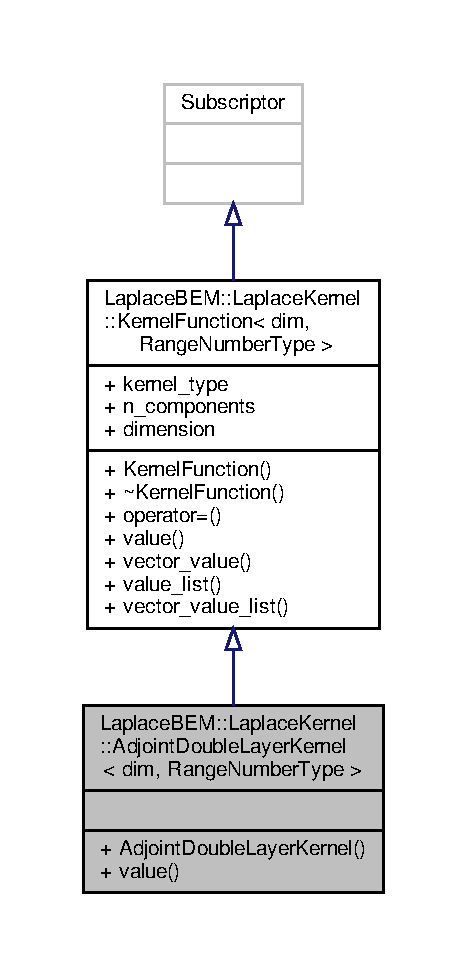
\includegraphics[width=224pt]{classLaplaceBEM_1_1LaplaceKernel_1_1AdjointDoubleLayerKernel__inherit__graph}
\end{center}
\end{figure}


Collaboration diagram for Laplace\+B\+EM\+:\+:Laplace\+Kernel\+:\+:Adjoint\+Double\+Layer\+Kernel$<$ dim, Range\+Number\+Type $>$\+:\nopagebreak
\begin{figure}[H]
\begin{center}
\leavevmode
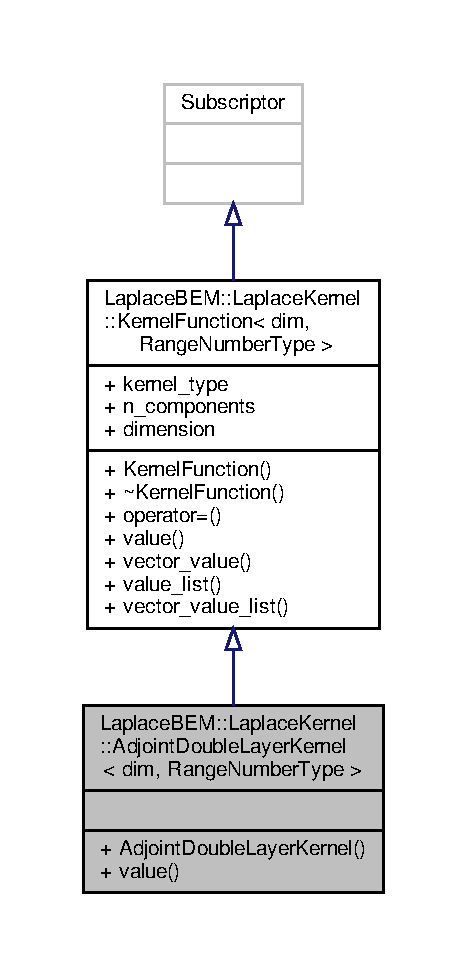
\includegraphics[width=224pt]{classLaplaceBEM_1_1LaplaceKernel_1_1AdjointDoubleLayerKernel__coll__graph}
\end{center}
\end{figure}
\subsection*{Public Member Functions}
\begin{DoxyCompactItemize}
\item 
virtual Range\+Number\+Type \hyperlink{classLaplaceBEM_1_1LaplaceKernel_1_1AdjointDoubleLayerKernel_acfa06279ea767680f2fbefee07a34304}{value} (const Point$<$ dim $>$ \&x, const Point$<$ dim $>$ \&y, const Tensor$<$ 1, dim $>$ \&nx, const Tensor$<$ 1, dim $>$ \&ny, const unsigned int component=0) const override
\end{DoxyCompactItemize}
\subsection*{Additional Inherited Members}


\subsection{Member Function Documentation}
\mbox{\Hypertarget{classLaplaceBEM_1_1LaplaceKernel_1_1AdjointDoubleLayerKernel_acfa06279ea767680f2fbefee07a34304}\label{classLaplaceBEM_1_1LaplaceKernel_1_1AdjointDoubleLayerKernel_acfa06279ea767680f2fbefee07a34304}} 
\index{Laplace\+B\+E\+M\+::\+Laplace\+Kernel\+::\+Adjoint\+Double\+Layer\+Kernel@{Laplace\+B\+E\+M\+::\+Laplace\+Kernel\+::\+Adjoint\+Double\+Layer\+Kernel}!value@{value}}
\index{value@{value}!Laplace\+B\+E\+M\+::\+Laplace\+Kernel\+::\+Adjoint\+Double\+Layer\+Kernel@{Laplace\+B\+E\+M\+::\+Laplace\+Kernel\+::\+Adjoint\+Double\+Layer\+Kernel}}
\subsubsection{\texorpdfstring{value()}{value()}}
{\footnotesize\ttfamily template$<$int dim, typename Range\+Number\+Type $>$ \\
Range\+Number\+Type \hyperlink{classLaplaceBEM_1_1LaplaceKernel_1_1AdjointDoubleLayerKernel}{Laplace\+B\+E\+M\+::\+Laplace\+Kernel\+::\+Adjoint\+Double\+Layer\+Kernel}$<$ dim, Range\+Number\+Type $>$\+::value (\begin{DoxyParamCaption}\item[{const Point$<$ dim $>$ \&}]{x,  }\item[{const Point$<$ dim $>$ \&}]{y,  }\item[{const Tensor$<$ 1, dim $>$ \&}]{nx,  }\item[{const Tensor$<$ 1, dim $>$ \&}]{ny,  }\item[{const unsigned int}]{component = {\ttfamily 0} }\end{DoxyParamCaption}) const\hspace{0.3cm}{\ttfamily [override]}, {\ttfamily [virtual]}}

Evaluate the kernel function at the specified point pair $(x, y)$ associated with their normal vectors $(n_x, n_y)$. In case the kernel function is vector-\/valued, this function only returns the required {\ttfamily component} in the result vector.


\begin{DoxyParams}{Parameters}
{\em x} & \\
\hline
{\em y} & \\
\hline
{\em nx} & \\
\hline
{\em ny} & \\
\hline
{\em component} & Component index in the result vector, if the kernel function is vector-\/valued. If the kernel function is scalar-\/valued, there is no such issue and {\ttfamily component} is 0 by default. \\
\hline
\end{DoxyParams}
\begin{DoxyReturn}{Returns}

\end{DoxyReturn}
This function should never be called, since as a member function of the abstract class, it has no literal definition of the function. Hence, we throw an error here.

Reimplemented from \hyperlink{classLaplaceBEM_1_1LaplaceKernel_1_1KernelFunction_aee6c638a4392616e89784d7b6558dd24}{Laplace\+B\+E\+M\+::\+Laplace\+Kernel\+::\+Kernel\+Function$<$ dim, Range\+Number\+Type $>$}.



The documentation for this class was generated from the following file\+:\begin{DoxyCompactItemize}
\item 
/home/jihuan/\+Projects/deal.\+ii/program/dealii-\/9.\+1.\+1/examples/laplace-\/bem/include/\hyperlink{laplace__bem_8h}{laplace\+\_\+bem.\+h}\end{DoxyCompactItemize}

\hypertarget{classLaplaceBEM_1_1Erichsen1996Efficient_1_1Example2_1_1AnalyticalSolution}{}\section{Laplace\+B\+EM\+:\+:Erichsen1996\+Efficient\+:\+:Example2\+:\+:Analytical\+Solution Class Reference}
\label{classLaplaceBEM_1_1Erichsen1996Efficient_1_1Example2_1_1AnalyticalSolution}\index{Laplace\+B\+E\+M\+::\+Erichsen1996\+Efficient\+::\+Example2\+::\+Analytical\+Solution@{Laplace\+B\+E\+M\+::\+Erichsen1996\+Efficient\+::\+Example2\+::\+Analytical\+Solution}}


Inheritance diagram for Laplace\+B\+EM\+:\+:Erichsen1996\+Efficient\+:\+:Example2\+:\+:Analytical\+Solution\+:\nopagebreak
\begin{figure}[H]
\begin{center}
\leavevmode
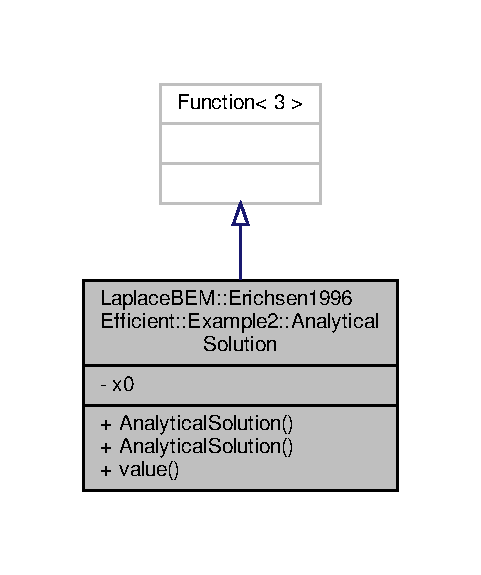
\includegraphics[width=231pt]{classLaplaceBEM_1_1Erichsen1996Efficient_1_1Example2_1_1AnalyticalSolution__inherit__graph}
\end{center}
\end{figure}


Collaboration diagram for Laplace\+B\+EM\+:\+:Erichsen1996\+Efficient\+:\+:Example2\+:\+:Analytical\+Solution\+:\nopagebreak
\begin{figure}[H]
\begin{center}
\leavevmode
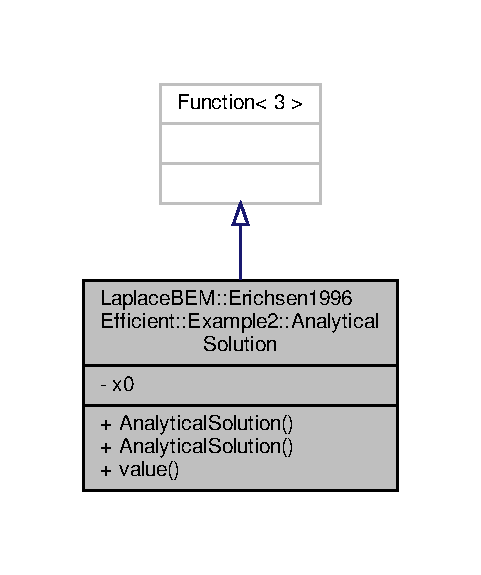
\includegraphics[width=231pt]{classLaplaceBEM_1_1Erichsen1996Efficient_1_1Example2_1_1AnalyticalSolution__coll__graph}
\end{center}
\end{figure}
\subsection*{Public Member Functions}
\begin{DoxyCompactItemize}
\item 
\mbox{\Hypertarget{classLaplaceBEM_1_1Erichsen1996Efficient_1_1Example2_1_1AnalyticalSolution_af37ad65fa1e788d7f2eda134752cb45d}\label{classLaplaceBEM_1_1Erichsen1996Efficient_1_1Example2_1_1AnalyticalSolution_af37ad65fa1e788d7f2eda134752cb45d}} 
{\bfseries Analytical\+Solution} (const Point$<$ 3 $>$ \&\hyperlink{classLaplaceBEM_1_1Erichsen1996Efficient_1_1Example2_1_1AnalyticalSolution_abc18babc7510cbb8228ae4382392bac8}{x0})
\item 
\mbox{\Hypertarget{classLaplaceBEM_1_1Erichsen1996Efficient_1_1Example2_1_1AnalyticalSolution_a8f1435b24dd481605b1655dc89459c3f}\label{classLaplaceBEM_1_1Erichsen1996Efficient_1_1Example2_1_1AnalyticalSolution_a8f1435b24dd481605b1655dc89459c3f}} 
double {\bfseries value} (const Point$<$ 3 $>$ \&p, const unsigned int component=0) const
\end{DoxyCompactItemize}
\subsection*{Private Attributes}
\begin{DoxyCompactItemize}
\item 
Point$<$ 3 $>$ \hyperlink{classLaplaceBEM_1_1Erichsen1996Efficient_1_1Example2_1_1AnalyticalSolution_abc18babc7510cbb8228ae4382392bac8}{x0}
\end{DoxyCompactItemize}


\subsection{Member Data Documentation}
\mbox{\Hypertarget{classLaplaceBEM_1_1Erichsen1996Efficient_1_1Example2_1_1AnalyticalSolution_abc18babc7510cbb8228ae4382392bac8}\label{classLaplaceBEM_1_1Erichsen1996Efficient_1_1Example2_1_1AnalyticalSolution_abc18babc7510cbb8228ae4382392bac8}} 
\index{Laplace\+B\+E\+M\+::\+Erichsen1996\+Efficient\+::\+Example2\+::\+Analytical\+Solution@{Laplace\+B\+E\+M\+::\+Erichsen1996\+Efficient\+::\+Example2\+::\+Analytical\+Solution}!x0@{x0}}
\index{x0@{x0}!Laplace\+B\+E\+M\+::\+Erichsen1996\+Efficient\+::\+Example2\+::\+Analytical\+Solution@{Laplace\+B\+E\+M\+::\+Erichsen1996\+Efficient\+::\+Example2\+::\+Analytical\+Solution}}
\subsubsection{\texorpdfstring{x0}{x0}}
{\footnotesize\ttfamily Point$<$3$>$ Laplace\+B\+E\+M\+::\+Erichsen1996\+Efficient\+::\+Example2\+::\+Analytical\+Solution\+::x0\hspace{0.3cm}{\ttfamily [private]}}

Location of the point source. 

The documentation for this class was generated from the following file\+:\begin{DoxyCompactItemize}
\item 
/home/jihuan/\+Projects/deal.\+ii/program/dealii-\/9.\+1.\+1/examples/laplace-\/bem/include/erichsen1996efficient\+\_\+example2.\+h\end{DoxyCompactItemize}

\hypertarget{classLaplaceBEM_1_1BEMValues}{}\section{Laplace\+B\+EM\+:\+:B\+E\+M\+Values$<$ dim, spacedim, Range\+Number\+Type $>$ Class Template Reference}
\label{classLaplaceBEM_1_1BEMValues}\index{Laplace\+B\+E\+M\+::\+B\+E\+M\+Values$<$ dim, spacedim, Range\+Number\+Type $>$@{Laplace\+B\+E\+M\+::\+B\+E\+M\+Values$<$ dim, spacedim, Range\+Number\+Type $>$}}


Collaboration diagram for Laplace\+B\+EM\+:\+:B\+E\+M\+Values$<$ dim, spacedim, Range\+Number\+Type $>$\+:\nopagebreak
\begin{figure}[H]
\begin{center}
\leavevmode
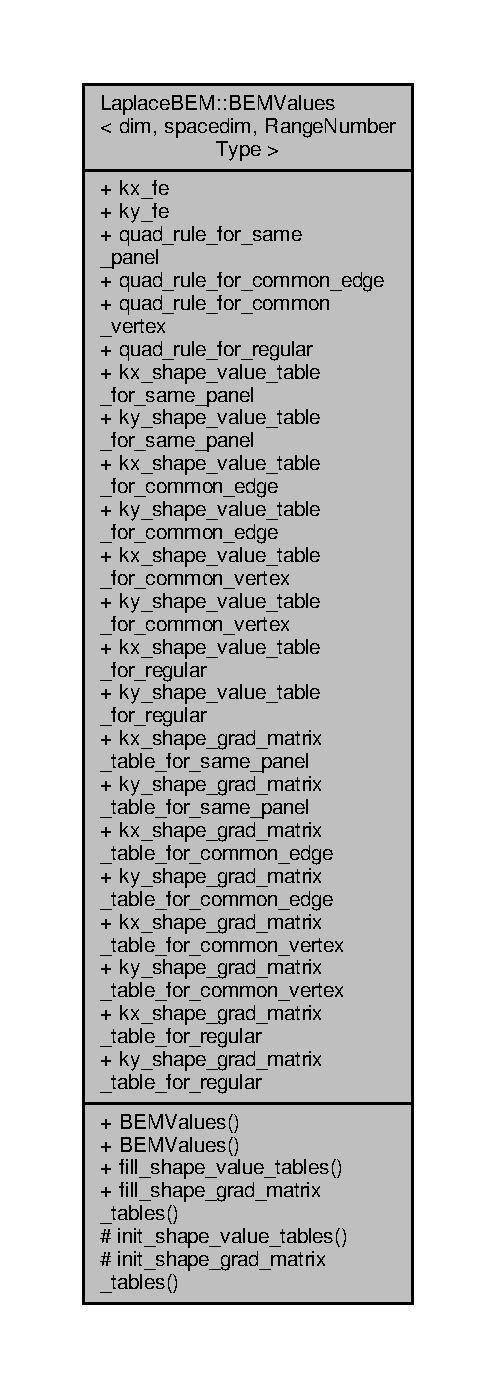
\includegraphics[height=550pt]{classLaplaceBEM_1_1BEMValues__coll__graph}
\end{center}
\end{figure}
\subsection*{Public Member Functions}
\begin{DoxyCompactItemize}
\item 
\mbox{\Hypertarget{classLaplaceBEM_1_1BEMValues_a7095a2e5448fa5478cc2d9affe319abf}\label{classLaplaceBEM_1_1BEMValues_a7095a2e5448fa5478cc2d9affe319abf}} 
{\bfseries B\+E\+M\+Values} (const Finite\+Element$<$ dim, spacedim $>$ \&kx\+\_\+fe, const Finite\+Element$<$ dim, spacedim $>$ \&ky\+\_\+fe, const Q\+Gauss$<$ 4 $>$ \&quad\+\_\+rule\+\_\+for\+\_\+same\+\_\+panel, const Q\+Gauss$<$ 4 $>$ \&quad\+\_\+rule\+\_\+for\+\_\+common\+\_\+edge, const Q\+Gauss$<$ 4 $>$ \&quad\+\_\+rule\+\_\+for\+\_\+common\+\_\+vertex, const Q\+Gauss$<$ 4 $>$ \&quad\+\_\+rule\+\_\+for\+\_\+regular)
\item 
\hyperlink{classLaplaceBEM_1_1BEMValues_ac40a849631e782f840a927e68bc2f9f6}{B\+E\+M\+Values} (const \hyperlink{classLaplaceBEM_1_1BEMValues}{B\+E\+M\+Values}$<$ dim, spacedim, Range\+Number\+Type $>$ \&bem\+\_\+values)
\item 
\mbox{\Hypertarget{classLaplaceBEM_1_1BEMValues_a3fd86680a51e688d003d5a0bfe09629f}\label{classLaplaceBEM_1_1BEMValues_a3fd86680a51e688d003d5a0bfe09629f}} 
void {\bfseries fill\+\_\+shape\+\_\+value\+\_\+tables} ()
\item 
\mbox{\Hypertarget{classLaplaceBEM_1_1BEMValues_a5383d5eb891f8cd742584e95aad976c8}\label{classLaplaceBEM_1_1BEMValues_a5383d5eb891f8cd742584e95aad976c8}} 
void {\bfseries fill\+\_\+shape\+\_\+grad\+\_\+matrix\+\_\+tables} ()
\end{DoxyCompactItemize}
\subsection*{Public Attributes}
\begin{DoxyCompactItemize}
\item 
\mbox{\Hypertarget{classLaplaceBEM_1_1BEMValues_aac76dabf40c054fb5a2608cf1a70d0df}\label{classLaplaceBEM_1_1BEMValues_aac76dabf40c054fb5a2608cf1a70d0df}} 
const Finite\+Element$<$ dim, spacedim $>$ \& {\bfseries kx\+\_\+fe}
\item 
\mbox{\Hypertarget{classLaplaceBEM_1_1BEMValues_a3b43f60bbc1d59238f201fa0e43325b4}\label{classLaplaceBEM_1_1BEMValues_a3b43f60bbc1d59238f201fa0e43325b4}} 
const Finite\+Element$<$ dim, spacedim $>$ \& {\bfseries ky\+\_\+fe}
\item 
\mbox{\Hypertarget{classLaplaceBEM_1_1BEMValues_aa6335f94192596e5512eee34aec37425}\label{classLaplaceBEM_1_1BEMValues_aa6335f94192596e5512eee34aec37425}} 
const Q\+Gauss$<$ 4 $>$ \& {\bfseries quad\+\_\+rule\+\_\+for\+\_\+same\+\_\+panel}
\item 
\mbox{\Hypertarget{classLaplaceBEM_1_1BEMValues_ab60f71cb70c2e1f437026e705ba81c45}\label{classLaplaceBEM_1_1BEMValues_ab60f71cb70c2e1f437026e705ba81c45}} 
const Q\+Gauss$<$ 4 $>$ \& {\bfseries quad\+\_\+rule\+\_\+for\+\_\+common\+\_\+edge}
\item 
\mbox{\Hypertarget{classLaplaceBEM_1_1BEMValues_afa138022ebdf7eac374f4f3da75d667b}\label{classLaplaceBEM_1_1BEMValues_afa138022ebdf7eac374f4f3da75d667b}} 
const Q\+Gauss$<$ 4 $>$ \& {\bfseries quad\+\_\+rule\+\_\+for\+\_\+common\+\_\+vertex}
\item 
\mbox{\Hypertarget{classLaplaceBEM_1_1BEMValues_a9639fb8cd2877d40d3142b4e43de00ce}\label{classLaplaceBEM_1_1BEMValues_a9639fb8cd2877d40d3142b4e43de00ce}} 
const Q\+Gauss$<$ 4 $>$ \& {\bfseries quad\+\_\+rule\+\_\+for\+\_\+regular}
\item 
\mbox{\Hypertarget{classLaplaceBEM_1_1BEMValues_a8e9a1d06a301dd95d70860159ecd990f}\label{classLaplaceBEM_1_1BEMValues_a8e9a1d06a301dd95d70860159ecd990f}} 
Table$<$ 3, Range\+Number\+Type $>$ {\bfseries kx\+\_\+shape\+\_\+value\+\_\+table\+\_\+for\+\_\+same\+\_\+panel}
\item 
\mbox{\Hypertarget{classLaplaceBEM_1_1BEMValues_a87347e8cacd41bf1ef0d83a2cf921889}\label{classLaplaceBEM_1_1BEMValues_a87347e8cacd41bf1ef0d83a2cf921889}} 
Table$<$ 3, Range\+Number\+Type $>$ {\bfseries ky\+\_\+shape\+\_\+value\+\_\+table\+\_\+for\+\_\+same\+\_\+panel}
\item 
\mbox{\Hypertarget{classLaplaceBEM_1_1BEMValues_a8a1e35a97b8b4868d16098f9997a9148}\label{classLaplaceBEM_1_1BEMValues_a8a1e35a97b8b4868d16098f9997a9148}} 
Table$<$ 3, Range\+Number\+Type $>$ {\bfseries kx\+\_\+shape\+\_\+value\+\_\+table\+\_\+for\+\_\+common\+\_\+edge}
\item 
\mbox{\Hypertarget{classLaplaceBEM_1_1BEMValues_a26a0c28bae67e71bcd8e5b58c22096d3}\label{classLaplaceBEM_1_1BEMValues_a26a0c28bae67e71bcd8e5b58c22096d3}} 
Table$<$ 3, Range\+Number\+Type $>$ {\bfseries ky\+\_\+shape\+\_\+value\+\_\+table\+\_\+for\+\_\+common\+\_\+edge}
\item 
\mbox{\Hypertarget{classLaplaceBEM_1_1BEMValues_a8d2e45be4d32bae87467a9b249ea1ae8}\label{classLaplaceBEM_1_1BEMValues_a8d2e45be4d32bae87467a9b249ea1ae8}} 
Table$<$ 3, Range\+Number\+Type $>$ {\bfseries kx\+\_\+shape\+\_\+value\+\_\+table\+\_\+for\+\_\+common\+\_\+vertex}
\item 
\mbox{\Hypertarget{classLaplaceBEM_1_1BEMValues_ad9ef63cf6509fa3916ddf835293baf39}\label{classLaplaceBEM_1_1BEMValues_ad9ef63cf6509fa3916ddf835293baf39}} 
Table$<$ 3, Range\+Number\+Type $>$ {\bfseries ky\+\_\+shape\+\_\+value\+\_\+table\+\_\+for\+\_\+common\+\_\+vertex}
\item 
\mbox{\Hypertarget{classLaplaceBEM_1_1BEMValues_aef7b057d9bb7d63d74ac30c34b0add62}\label{classLaplaceBEM_1_1BEMValues_aef7b057d9bb7d63d74ac30c34b0add62}} 
Table$<$ 3, Range\+Number\+Type $>$ {\bfseries kx\+\_\+shape\+\_\+value\+\_\+table\+\_\+for\+\_\+regular}
\item 
\mbox{\Hypertarget{classLaplaceBEM_1_1BEMValues_aec5f9fa16be14831e124275fe74921f0}\label{classLaplaceBEM_1_1BEMValues_aec5f9fa16be14831e124275fe74921f0}} 
Table$<$ 3, Range\+Number\+Type $>$ {\bfseries ky\+\_\+shape\+\_\+value\+\_\+table\+\_\+for\+\_\+regular}
\item 
\mbox{\Hypertarget{classLaplaceBEM_1_1BEMValues_a66a2d68e7fbc709fbca53c5d3158b288}\label{classLaplaceBEM_1_1BEMValues_a66a2d68e7fbc709fbca53c5d3158b288}} 
Table$<$ 2, Full\+Matrix$<$ Range\+Number\+Type $>$ $>$ {\bfseries kx\+\_\+shape\+\_\+grad\+\_\+matrix\+\_\+table\+\_\+for\+\_\+same\+\_\+panel}
\item 
\mbox{\Hypertarget{classLaplaceBEM_1_1BEMValues_aea315427a1f1fec575cf6b9710907747}\label{classLaplaceBEM_1_1BEMValues_aea315427a1f1fec575cf6b9710907747}} 
Table$<$ 2, Full\+Matrix$<$ Range\+Number\+Type $>$ $>$ {\bfseries ky\+\_\+shape\+\_\+grad\+\_\+matrix\+\_\+table\+\_\+for\+\_\+same\+\_\+panel}
\item 
\mbox{\Hypertarget{classLaplaceBEM_1_1BEMValues_ae25c2dc5d9aa6c4dfd5c05b41197a7ef}\label{classLaplaceBEM_1_1BEMValues_ae25c2dc5d9aa6c4dfd5c05b41197a7ef}} 
Table$<$ 2, Full\+Matrix$<$ Range\+Number\+Type $>$ $>$ {\bfseries kx\+\_\+shape\+\_\+grad\+\_\+matrix\+\_\+table\+\_\+for\+\_\+common\+\_\+edge}
\item 
\mbox{\Hypertarget{classLaplaceBEM_1_1BEMValues_ae30c6f5629a6aebd6cf2445f7dc7357f}\label{classLaplaceBEM_1_1BEMValues_ae30c6f5629a6aebd6cf2445f7dc7357f}} 
Table$<$ 2, Full\+Matrix$<$ Range\+Number\+Type $>$ $>$ {\bfseries ky\+\_\+shape\+\_\+grad\+\_\+matrix\+\_\+table\+\_\+for\+\_\+common\+\_\+edge}
\item 
\mbox{\Hypertarget{classLaplaceBEM_1_1BEMValues_af272687194bb9836a8e54ae25e2ef538}\label{classLaplaceBEM_1_1BEMValues_af272687194bb9836a8e54ae25e2ef538}} 
Table$<$ 2, Full\+Matrix$<$ Range\+Number\+Type $>$ $>$ {\bfseries kx\+\_\+shape\+\_\+grad\+\_\+matrix\+\_\+table\+\_\+for\+\_\+common\+\_\+vertex}
\item 
\mbox{\Hypertarget{classLaplaceBEM_1_1BEMValues_a86ef4b138039af89dc71569bbf18a711}\label{classLaplaceBEM_1_1BEMValues_a86ef4b138039af89dc71569bbf18a711}} 
Table$<$ 2, Full\+Matrix$<$ Range\+Number\+Type $>$ $>$ {\bfseries ky\+\_\+shape\+\_\+grad\+\_\+matrix\+\_\+table\+\_\+for\+\_\+common\+\_\+vertex}
\item 
\mbox{\Hypertarget{classLaplaceBEM_1_1BEMValues_a34933185cecf9d4cea46597642f8d802}\label{classLaplaceBEM_1_1BEMValues_a34933185cecf9d4cea46597642f8d802}} 
Table$<$ 2, Full\+Matrix$<$ Range\+Number\+Type $>$ $>$ {\bfseries kx\+\_\+shape\+\_\+grad\+\_\+matrix\+\_\+table\+\_\+for\+\_\+regular}
\item 
\mbox{\Hypertarget{classLaplaceBEM_1_1BEMValues_ad6938f3aad2ab93ed61fc48de8e4de65}\label{classLaplaceBEM_1_1BEMValues_ad6938f3aad2ab93ed61fc48de8e4de65}} 
Table$<$ 2, Full\+Matrix$<$ Range\+Number\+Type $>$ $>$ {\bfseries ky\+\_\+shape\+\_\+grad\+\_\+matrix\+\_\+table\+\_\+for\+\_\+regular}
\end{DoxyCompactItemize}
\subsection*{Protected Member Functions}
\begin{DoxyCompactItemize}
\item 
\mbox{\Hypertarget{classLaplaceBEM_1_1BEMValues_a71328aee0f80bcea63897444b086de99}\label{classLaplaceBEM_1_1BEMValues_a71328aee0f80bcea63897444b086de99}} 
void {\bfseries init\+\_\+shape\+\_\+value\+\_\+tables} ()
\item 
\mbox{\Hypertarget{classLaplaceBEM_1_1BEMValues_a5646d3caf1ede82b5dca1f82be893dd4}\label{classLaplaceBEM_1_1BEMValues_a5646d3caf1ede82b5dca1f82be893dd4}} 
void {\bfseries init\+\_\+shape\+\_\+grad\+\_\+matrix\+\_\+tables} ()
\end{DoxyCompactItemize}


\subsection{Constructor \& Destructor Documentation}
\mbox{\Hypertarget{classLaplaceBEM_1_1BEMValues_ac40a849631e782f840a927e68bc2f9f6}\label{classLaplaceBEM_1_1BEMValues_ac40a849631e782f840a927e68bc2f9f6}} 
\index{Laplace\+B\+E\+M\+::\+B\+E\+M\+Values@{Laplace\+B\+E\+M\+::\+B\+E\+M\+Values}!B\+E\+M\+Values@{B\+E\+M\+Values}}
\index{B\+E\+M\+Values@{B\+E\+M\+Values}!Laplace\+B\+E\+M\+::\+B\+E\+M\+Values@{Laplace\+B\+E\+M\+::\+B\+E\+M\+Values}}
\subsubsection{\texorpdfstring{B\+E\+M\+Values()}{BEMValues()}}
{\footnotesize\ttfamily template$<$int dim, int spacedim, typename Range\+Number\+Type $>$ \\
\hyperlink{classLaplaceBEM_1_1BEMValues}{Laplace\+B\+E\+M\+::\+B\+E\+M\+Values}$<$ dim, spacedim, Range\+Number\+Type $>$\+::\hyperlink{classLaplaceBEM_1_1BEMValues}{B\+E\+M\+Values} (\begin{DoxyParamCaption}\item[{const \hyperlink{classLaplaceBEM_1_1BEMValues}{B\+E\+M\+Values}$<$ dim, spacedim, Range\+Number\+Type $>$ \&}]{bem\+\_\+values }\end{DoxyParamCaption})}

Copy constructor for class {\ttfamily \hyperlink{classLaplaceBEM_1_1BEMValues}{B\+E\+M\+Values}}. 
\begin{DoxyParams}{Parameters}
{\em bem\+\_\+values} & \\
\hline
\end{DoxyParams}


References Laplace\+B\+E\+M\+::bem\+\_\+shape\+\_\+grad\+\_\+matrices\+\_\+common\+\_\+edge(), Laplace\+B\+E\+M\+::bem\+\_\+shape\+\_\+grad\+\_\+matrices\+\_\+common\+\_\+vertex(), Laplace\+B\+E\+M\+::bem\+\_\+shape\+\_\+grad\+\_\+matrices\+\_\+regular(), Laplace\+B\+E\+M\+::bem\+\_\+shape\+\_\+grad\+\_\+matrices\+\_\+same\+\_\+panel(), Laplace\+B\+E\+M\+::bem\+\_\+shape\+\_\+values\+\_\+common\+\_\+edge(), Laplace\+B\+E\+M\+::bem\+\_\+shape\+\_\+values\+\_\+common\+\_\+vertex(), Laplace\+B\+E\+M\+::bem\+\_\+shape\+\_\+values\+\_\+regular(), and Laplace\+B\+E\+M\+::bem\+\_\+shape\+\_\+values\+\_\+same\+\_\+panel().



The documentation for this class was generated from the following file\+:\begin{DoxyCompactItemize}
\item 
/home/jihuan/\+Projects/deal.\+ii/program/dealii-\/9.\+1.\+1/examples/laplace-\/bem/include/\hyperlink{laplace__bem_8h}{laplace\+\_\+bem.\+h}\end{DoxyCompactItemize}

\hypertarget{classBinaryTreeNode}{}\section{Binary\+Tree\+Node$<$ T $>$ Class Template Reference}
\label{classBinaryTreeNode}\index{Binary\+Tree\+Node$<$ T $>$@{Binary\+Tree\+Node$<$ T $>$}}


Class for binary tree node.  




{\ttfamily \#include $<$tree.\+h$>$}



Inheritance diagram for Binary\+Tree\+Node$<$ T $>$\+:\nopagebreak
\begin{figure}[H]
\begin{center}
\leavevmode
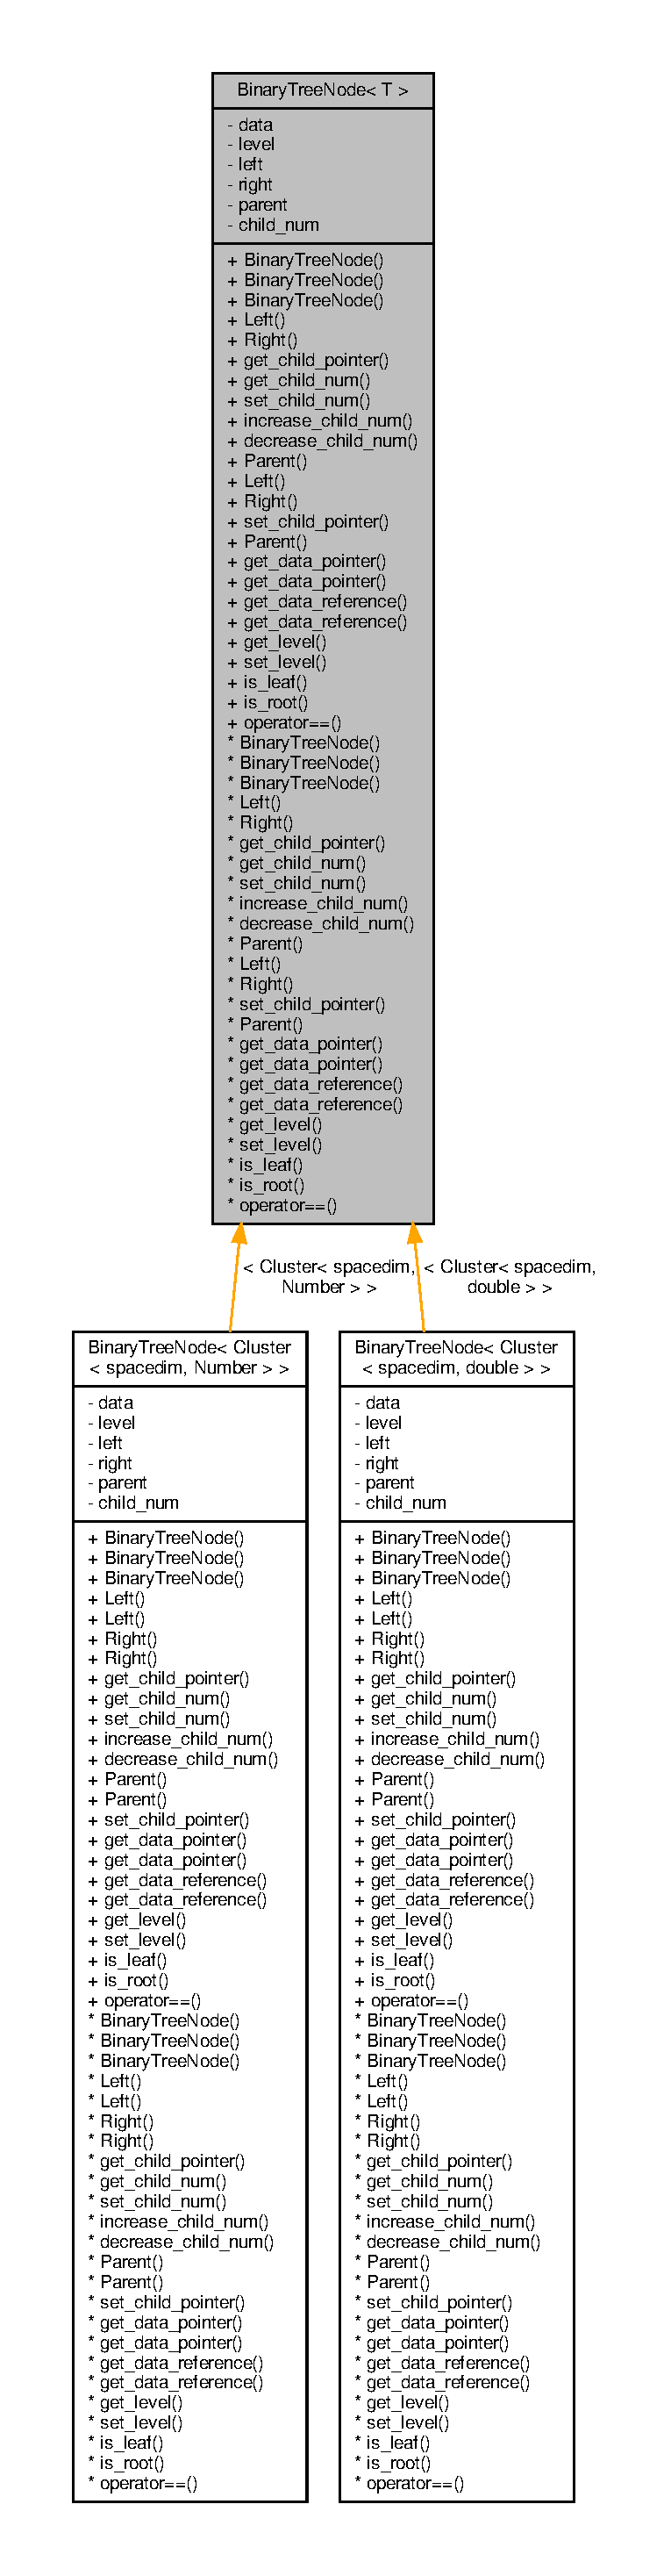
\includegraphics[height=550pt]{classBinaryTreeNode__inherit__graph}
\end{center}
\end{figure}


Collaboration diagram for Binary\+Tree\+Node$<$ T $>$\+:\nopagebreak
\begin{figure}[H]
\begin{center}
\leavevmode
\includegraphics[height=550pt]{classBinaryTreeNode__coll__graph}
\end{center}
\end{figure}
\subsection*{Public Member Functions}
\textbf{ }\par
\begin{DoxyCompactItemize}
\item 
\hyperlink{classBinaryTreeNode_aa7a20e203a1e6aa2cf59be86bd493f08}{Binary\+Tree\+Node} ()
\item 
\hyperlink{classBinaryTreeNode_a44089b64b058a805e5f17d9518317f38}{Binary\+Tree\+Node} (const \hyperlink{classBinaryTreeNode}{Binary\+Tree\+Node} \&node)
\item 
\hyperlink{classBinaryTreeNode_adc784168efc0f866e0c5eb368cfec60e}{Binary\+Tree\+Node} (const T \&data, unsigned int level, \hyperlink{classBinaryTreeNode}{Binary\+Tree\+Node} $\ast$left=nullptr, \hyperlink{classBinaryTreeNode}{Binary\+Tree\+Node} $\ast$right=nullptr, \hyperlink{classBinaryTreeNode}{Binary\+Tree\+Node} $\ast$parent=nullptr)
\item 
\hyperlink{classBinaryTreeNode}{Binary\+Tree\+Node} $\ast$ \hyperlink{classBinaryTreeNode_af72f5be84f4ac9fa158718032cada52a}{Left} (void) const
\item 
\hyperlink{classBinaryTreeNode}{Binary\+Tree\+Node} $\ast$ \hyperlink{classBinaryTreeNode_ade872fc08f12c154c28c934a3991ae08}{Right} (void) const
\item 
\hyperlink{classBinaryTreeNode}{Binary\+Tree\+Node} $\ast$ \hyperlink{classBinaryTreeNode_a2ef0648ec3a937f4153a877b0e47eaa5}{get\+\_\+child\+\_\+pointer} (std\+::size\+\_\+t index) const
\item 
unsigned int \hyperlink{classBinaryTreeNode_a41d03ea4bdbb686094273fa47c7f988a}{get\+\_\+child\+\_\+num} () const
\item 
void \hyperlink{classBinaryTreeNode_ae9c5a478fed2c72e7aa9f2b28a0010e7}{set\+\_\+child\+\_\+num} (const unsigned int \hyperlink{classBinaryTreeNode_a434bfe00afd0b3dc86943e138f49fc3d}{child\+\_\+num})
\item 
void \hyperlink{classBinaryTreeNode_a0c22f12230f685c522ab80484ce4ce7f}{increase\+\_\+child\+\_\+num} (const unsigned int incr\+\_\+num=1)
\item 
void \hyperlink{classBinaryTreeNode_a05dfef5724e65a69494ac91d40852bde}{decrease\+\_\+child\+\_\+num} (const unsigned int decr\+\_\+num=1)
\item 
\hyperlink{classBinaryTreeNode}{Binary\+Tree\+Node} $\ast$ \hyperlink{classBinaryTreeNode_a2eea9d71ae776d02b23bb9f3869f0f6d}{Parent} (void) const
\item 
void \hyperlink{classBinaryTreeNode_aa645c65bfa4702e04c97d70c37632a17}{Left} (const \hyperlink{classBinaryTreeNode}{Binary\+Tree\+Node} $\ast$node\+\_\+pointer)
\item 
void \hyperlink{classBinaryTreeNode_add14f066fd229ef84f334110ebc0061f}{Right} (const \hyperlink{classBinaryTreeNode}{Binary\+Tree\+Node} $\ast$node\+\_\+pointer)
\item 
void \hyperlink{classBinaryTreeNode_a37f0dd5197e454f14e3e99c85ab516eb}{set\+\_\+child\+\_\+pointer} (std\+::size\+\_\+t index, const \hyperlink{classBinaryTreeNode}{Binary\+Tree\+Node} $\ast$node\+\_\+pointer)
\item 
void \hyperlink{classBinaryTreeNode_abd72fc34f46fb41abdf9a692b4db0cdd}{Parent} (const \hyperlink{classBinaryTreeNode}{Binary\+Tree\+Node} $\ast$node\+\_\+pointer)
\item 
T $\ast$ \hyperlink{classBinaryTreeNode_aee6acddfb9686de160994b81a32faa80}{get\+\_\+data\+\_\+pointer} ()
\item 
const T $\ast$ \hyperlink{classBinaryTreeNode_acb9eb20251b6fdde199264527499c9ca}{get\+\_\+data\+\_\+pointer} () const
\item 
T \& \hyperlink{classBinaryTreeNode_ad24220a78b219a242dc66be86cf6ddd9}{get\+\_\+data\+\_\+reference} ()
\item 
const T \& \hyperlink{classBinaryTreeNode_a6bfbb8840c8a263ffcaacb0b7b61170c}{get\+\_\+data\+\_\+reference} () const
\item 
unsigned int \hyperlink{classBinaryTreeNode_aa89de0a58ae53ae5eb701bec3adc880a}{get\+\_\+level} () const
\item 
void \hyperlink{classBinaryTreeNode_ae420da1d4c6a4ac054cd181535e718f2}{set\+\_\+level} (const unsigned int level)
\item 
bool \hyperlink{classBinaryTreeNode_a9ef9e129737446b961cafd353b0a7370}{is\+\_\+leaf} () const
\item 
bool \hyperlink{classBinaryTreeNode_a7f24a34754ef61fb41004606a26cc7e1}{is\+\_\+root} () const
\item 
bool \hyperlink{classBinaryTreeNode_a0a362a295603c8dfffb45663e3c89507}{operator==} (const \hyperlink{classBinaryTreeNode}{Binary\+Tree\+Node}$<$ T $>$ \&node) const
\end{DoxyCompactItemize}

\subsection*{Private Attributes}
\begin{DoxyCompactItemize}
\item 
\mbox{\Hypertarget{classBinaryTreeNode_aefbcb5264485f5b637c3b25b370af450}\label{classBinaryTreeNode_aefbcb5264485f5b637c3b25b370af450}} 
T {\bfseries data}
\item 
\mbox{\Hypertarget{classBinaryTreeNode_af87f0bd6700c5d12815563da41e0b2f0}\label{classBinaryTreeNode_af87f0bd6700c5d12815563da41e0b2f0}} 
unsigned int {\bfseries level}
\item 
\mbox{\Hypertarget{classBinaryTreeNode_af3c06a27fffe0b35e83e1a7b717e042e}\label{classBinaryTreeNode_af3c06a27fffe0b35e83e1a7b717e042e}} 
\hyperlink{classBinaryTreeNode}{Binary\+Tree\+Node} $\ast$ {\bfseries left}
\item 
\mbox{\Hypertarget{classBinaryTreeNode_acbe239a79828451cbdd38730995d9e89}\label{classBinaryTreeNode_acbe239a79828451cbdd38730995d9e89}} 
\hyperlink{classBinaryTreeNode}{Binary\+Tree\+Node} $\ast$ {\bfseries right}
\item 
\mbox{\Hypertarget{classBinaryTreeNode_a55abb0ef30f3951450f3a22f030b6149}\label{classBinaryTreeNode_a55abb0ef30f3951450f3a22f030b6149}} 
\hyperlink{classBinaryTreeNode}{Binary\+Tree\+Node} $\ast$ {\bfseries parent}
\item 
unsigned int \hyperlink{classBinaryTreeNode_a434bfe00afd0b3dc86943e138f49fc3d}{child\+\_\+num}
\end{DoxyCompactItemize}


\subsection{Detailed Description}
\subsubsection*{template$<$typename T$>$\newline
class Binary\+Tree\+Node$<$ T $>$}

Class for binary tree node. 

In the implementation of hierarchical matrices, a binary tree node is designed to hold a cluster (\hyperlink{classCluster}{Cluster}) in a cluster tree (\hyperlink{classClusterTree}{Cluster\+Tree}) along with two pointers {\ttfamily left} and {\ttfamily right} pointing to the two children belong to the node itself. The template argument {\ttfamily T} should be assigned the type of the cluster. 

\subsection{Constructor \& Destructor Documentation}
\mbox{\Hypertarget{classBinaryTreeNode_aa7a20e203a1e6aa2cf59be86bd493f08}\label{classBinaryTreeNode_aa7a20e203a1e6aa2cf59be86bd493f08}} 
\index{Binary\+Tree\+Node@{Binary\+Tree\+Node}!Binary\+Tree\+Node@{Binary\+Tree\+Node}}
\index{Binary\+Tree\+Node@{Binary\+Tree\+Node}!Binary\+Tree\+Node@{Binary\+Tree\+Node}}
\subsubsection{\texorpdfstring{Binary\+Tree\+Node()}{BinaryTreeNode()}\hspace{0.1cm}{\footnotesize\ttfamily [1/3]}}
{\footnotesize\ttfamily template$<$typename T $>$ \\
\hyperlink{classBinaryTreeNode}{Binary\+Tree\+Node}$<$ T $>$\+::\hyperlink{classBinaryTreeNode}{Binary\+Tree\+Node} (\begin{DoxyParamCaption}{ }\end{DoxyParamCaption})}

Default constructor. \mbox{\Hypertarget{classBinaryTreeNode_a44089b64b058a805e5f17d9518317f38}\label{classBinaryTreeNode_a44089b64b058a805e5f17d9518317f38}} 
\index{Binary\+Tree\+Node@{Binary\+Tree\+Node}!Binary\+Tree\+Node@{Binary\+Tree\+Node}}
\index{Binary\+Tree\+Node@{Binary\+Tree\+Node}!Binary\+Tree\+Node@{Binary\+Tree\+Node}}
\subsubsection{\texorpdfstring{Binary\+Tree\+Node()}{BinaryTreeNode()}\hspace{0.1cm}{\footnotesize\ttfamily [2/3]}}
{\footnotesize\ttfamily template$<$typename T $>$ \\
\hyperlink{classBinaryTreeNode}{Binary\+Tree\+Node}$<$ T $>$\+::\hyperlink{classBinaryTreeNode}{Binary\+Tree\+Node} (\begin{DoxyParamCaption}\item[{const \hyperlink{classBinaryTreeNode}{Binary\+Tree\+Node}$<$ T $>$ \&}]{node }\end{DoxyParamCaption})}

Copy constructor. \mbox{\Hypertarget{classBinaryTreeNode_adc784168efc0f866e0c5eb368cfec60e}\label{classBinaryTreeNode_adc784168efc0f866e0c5eb368cfec60e}} 
\index{Binary\+Tree\+Node@{Binary\+Tree\+Node}!Binary\+Tree\+Node@{Binary\+Tree\+Node}}
\index{Binary\+Tree\+Node@{Binary\+Tree\+Node}!Binary\+Tree\+Node@{Binary\+Tree\+Node}}
\subsubsection{\texorpdfstring{Binary\+Tree\+Node()}{BinaryTreeNode()}\hspace{0.1cm}{\footnotesize\ttfamily [3/3]}}
{\footnotesize\ttfamily template$<$typename T$>$ \\
\hyperlink{classBinaryTreeNode}{Binary\+Tree\+Node}$<$ T $>$\+::\hyperlink{classBinaryTreeNode}{Binary\+Tree\+Node} (\begin{DoxyParamCaption}\item[{const T \&}]{data,  }\item[{unsigned int}]{level,  }\item[{\hyperlink{classBinaryTreeNode}{Binary\+Tree\+Node}$<$ T $>$ $\ast$}]{left = {\ttfamily nullptr},  }\item[{\hyperlink{classBinaryTreeNode}{Binary\+Tree\+Node}$<$ T $>$ $\ast$}]{right = {\ttfamily nullptr},  }\item[{\hyperlink{classBinaryTreeNode}{Binary\+Tree\+Node}$<$ T $>$ $\ast$}]{parent = {\ttfamily nullptr} }\end{DoxyParamCaption})}

Constructor from the given data.

N.\+B. The data of type {\ttfamily T} will be copied into the created node. Increment the {\ttfamily child\+\_\+num} of the parent node.

\subsection{Member Function Documentation}
\mbox{\Hypertarget{classBinaryTreeNode_a05dfef5724e65a69494ac91d40852bde}\label{classBinaryTreeNode_a05dfef5724e65a69494ac91d40852bde}} 
\index{Binary\+Tree\+Node@{Binary\+Tree\+Node}!decrease\+\_\+child\+\_\+num@{decrease\+\_\+child\+\_\+num}}
\index{decrease\+\_\+child\+\_\+num@{decrease\+\_\+child\+\_\+num}!Binary\+Tree\+Node@{Binary\+Tree\+Node}}
\subsubsection{\texorpdfstring{decrease\+\_\+child\+\_\+num()}{decrease\_child\_num()}}
{\footnotesize\ttfamily template$<$typename T $>$ \\
void \hyperlink{classBinaryTreeNode}{Binary\+Tree\+Node}$<$ T $>$\+::decrease\+\_\+child\+\_\+num (\begin{DoxyParamCaption}\item[{const unsigned int}]{decr\+\_\+num = {\ttfamily 1} }\end{DoxyParamCaption})}

Decrease the total number of children. \begin{DoxyReturn}{Returns}

\end{DoxyReturn}
\mbox{\Hypertarget{classBinaryTreeNode_a41d03ea4bdbb686094273fa47c7f988a}\label{classBinaryTreeNode_a41d03ea4bdbb686094273fa47c7f988a}} 
\index{Binary\+Tree\+Node@{Binary\+Tree\+Node}!get\+\_\+child\+\_\+num@{get\+\_\+child\+\_\+num}}
\index{get\+\_\+child\+\_\+num@{get\+\_\+child\+\_\+num}!Binary\+Tree\+Node@{Binary\+Tree\+Node}}
\subsubsection{\texorpdfstring{get\+\_\+child\+\_\+num()}{get\_child\_num()}}
{\footnotesize\ttfamily template$<$typename T $>$ \\
unsigned int \hyperlink{classBinaryTreeNode}{Binary\+Tree\+Node}$<$ T $>$\+::get\+\_\+child\+\_\+num (\begin{DoxyParamCaption}{ }\end{DoxyParamCaption}) const}

Get the total number of nonempty children. 

Referenced by Get\+Tree\+Leaves(), and Print\+Tree\+Node().

\mbox{\Hypertarget{classBinaryTreeNode_a2ef0648ec3a937f4153a877b0e47eaa5}\label{classBinaryTreeNode_a2ef0648ec3a937f4153a877b0e47eaa5}} 
\index{Binary\+Tree\+Node@{Binary\+Tree\+Node}!get\+\_\+child\+\_\+pointer@{get\+\_\+child\+\_\+pointer}}
\index{get\+\_\+child\+\_\+pointer@{get\+\_\+child\+\_\+pointer}!Binary\+Tree\+Node@{Binary\+Tree\+Node}}
\subsubsection{\texorpdfstring{get\+\_\+child\+\_\+pointer()}{get\_child\_pointer()}}
{\footnotesize\ttfamily template$<$typename T $>$ \\
\hyperlink{classBinaryTreeNode}{Binary\+Tree\+Node}$<$ T $>$ $\ast$ \hyperlink{classBinaryTreeNode}{Binary\+Tree\+Node}$<$ T $>$\+::get\+\_\+child\+\_\+pointer (\begin{DoxyParamCaption}\item[{std\+::size\+\_\+t}]{index }\end{DoxyParamCaption}) const}

Get the pointer to the {\ttfamily index\textquotesingle{}th} child. 
\begin{DoxyParams}{Parameters}
{\em index} & Index of the child \\
\hline
\end{DoxyParams}
\begin{DoxyReturn}{Returns}

\end{DoxyReturn}
\mbox{\Hypertarget{classBinaryTreeNode_aee6acddfb9686de160994b81a32faa80}\label{classBinaryTreeNode_aee6acddfb9686de160994b81a32faa80}} 
\index{Binary\+Tree\+Node@{Binary\+Tree\+Node}!get\+\_\+data\+\_\+pointer@{get\+\_\+data\+\_\+pointer}}
\index{get\+\_\+data\+\_\+pointer@{get\+\_\+data\+\_\+pointer}!Binary\+Tree\+Node@{Binary\+Tree\+Node}}
\subsubsection{\texorpdfstring{get\+\_\+data\+\_\+pointer()}{get\_data\_pointer()}\hspace{0.1cm}{\footnotesize\ttfamily [1/2]}}
{\footnotesize\ttfamily template$<$typename T $>$ \\
T $\ast$ \hyperlink{classBinaryTreeNode}{Binary\+Tree\+Node}$<$ T $>$\+::get\+\_\+data\+\_\+pointer (\begin{DoxyParamCaption}{ }\end{DoxyParamCaption})}

Get the pointer to the node data. 

Referenced by Cluster\+Tree$<$ spacedim, Number $>$\+::partition\+\_\+from\+\_\+cluster\+\_\+node().

\mbox{\Hypertarget{classBinaryTreeNode_acb9eb20251b6fdde199264527499c9ca}\label{classBinaryTreeNode_acb9eb20251b6fdde199264527499c9ca}} 
\index{Binary\+Tree\+Node@{Binary\+Tree\+Node}!get\+\_\+data\+\_\+pointer@{get\+\_\+data\+\_\+pointer}}
\index{get\+\_\+data\+\_\+pointer@{get\+\_\+data\+\_\+pointer}!Binary\+Tree\+Node@{Binary\+Tree\+Node}}
\subsubsection{\texorpdfstring{get\+\_\+data\+\_\+pointer()}{get\_data\_pointer()}\hspace{0.1cm}{\footnotesize\ttfamily [2/2]}}
{\footnotesize\ttfamily template$<$typename T $>$ \\
const T $\ast$ \hyperlink{classBinaryTreeNode}{Binary\+Tree\+Node}$<$ T $>$\+::get\+\_\+data\+\_\+pointer (\begin{DoxyParamCaption}{ }\end{DoxyParamCaption}) const}

Get the pointer to the node data (const version). \mbox{\Hypertarget{classBinaryTreeNode_ad24220a78b219a242dc66be86cf6ddd9}\label{classBinaryTreeNode_ad24220a78b219a242dc66be86cf6ddd9}} 
\index{Binary\+Tree\+Node@{Binary\+Tree\+Node}!get\+\_\+data\+\_\+reference@{get\+\_\+data\+\_\+reference}}
\index{get\+\_\+data\+\_\+reference@{get\+\_\+data\+\_\+reference}!Binary\+Tree\+Node@{Binary\+Tree\+Node}}
\subsubsection{\texorpdfstring{get\+\_\+data\+\_\+reference()}{get\_data\_reference()}\hspace{0.1cm}{\footnotesize\ttfamily [1/2]}}
{\footnotesize\ttfamily template$<$typename T $>$ \\
T \& \hyperlink{classBinaryTreeNode}{Binary\+Tree\+Node}$<$ T $>$\+::get\+\_\+data\+\_\+reference (\begin{DoxyParamCaption}{ }\end{DoxyParamCaption})}

Get the reference to the node data. 

Referenced by Copy\+Tree(), and Print\+Tree\+Node().

\mbox{\Hypertarget{classBinaryTreeNode_a6bfbb8840c8a263ffcaacb0b7b61170c}\label{classBinaryTreeNode_a6bfbb8840c8a263ffcaacb0b7b61170c}} 
\index{Binary\+Tree\+Node@{Binary\+Tree\+Node}!get\+\_\+data\+\_\+reference@{get\+\_\+data\+\_\+reference}}
\index{get\+\_\+data\+\_\+reference@{get\+\_\+data\+\_\+reference}!Binary\+Tree\+Node@{Binary\+Tree\+Node}}
\subsubsection{\texorpdfstring{get\+\_\+data\+\_\+reference()}{get\_data\_reference()}\hspace{0.1cm}{\footnotesize\ttfamily [2/2]}}
{\footnotesize\ttfamily template$<$typename T $>$ \\
const T \& \hyperlink{classBinaryTreeNode}{Binary\+Tree\+Node}$<$ T $>$\+::get\+\_\+data\+\_\+reference (\begin{DoxyParamCaption}{ }\end{DoxyParamCaption}) const}

Get the reference to the node data (const version). \mbox{\Hypertarget{classBinaryTreeNode_aa89de0a58ae53ae5eb701bec3adc880a}\label{classBinaryTreeNode_aa89de0a58ae53ae5eb701bec3adc880a}} 
\index{Binary\+Tree\+Node@{Binary\+Tree\+Node}!get\+\_\+level@{get\+\_\+level}}
\index{get\+\_\+level@{get\+\_\+level}!Binary\+Tree\+Node@{Binary\+Tree\+Node}}
\subsubsection{\texorpdfstring{get\+\_\+level()}{get\_level()}}
{\footnotesize\ttfamily template$<$typename T $>$ \\
unsigned int \hyperlink{classBinaryTreeNode}{Binary\+Tree\+Node}$<$ T $>$\+::get\+\_\+level (\begin{DoxyParamCaption}{ }\end{DoxyParamCaption}) const}

Get the level of the node in the tree. 

Referenced by Copy\+Tree(), Cluster\+Tree$<$ spacedim, Number $>$\+::partition\+\_\+from\+\_\+cluster\+\_\+node(), and Print\+Tree\+Node().

\mbox{\Hypertarget{classBinaryTreeNode_a0c22f12230f685c522ab80484ce4ce7f}\label{classBinaryTreeNode_a0c22f12230f685c522ab80484ce4ce7f}} 
\index{Binary\+Tree\+Node@{Binary\+Tree\+Node}!increase\+\_\+child\+\_\+num@{increase\+\_\+child\+\_\+num}}
\index{increase\+\_\+child\+\_\+num@{increase\+\_\+child\+\_\+num}!Binary\+Tree\+Node@{Binary\+Tree\+Node}}
\subsubsection{\texorpdfstring{increase\+\_\+child\+\_\+num()}{increase\_child\_num()}}
{\footnotesize\ttfamily template$<$typename T $>$ \\
void \hyperlink{classBinaryTreeNode}{Binary\+Tree\+Node}$<$ T $>$\+::increase\+\_\+child\+\_\+num (\begin{DoxyParamCaption}\item[{const unsigned int}]{incr\+\_\+num = {\ttfamily 1} }\end{DoxyParamCaption})}

Increase the total number of children. 

Referenced by Copy\+Tree().

\mbox{\Hypertarget{classBinaryTreeNode_a9ef9e129737446b961cafd353b0a7370}\label{classBinaryTreeNode_a9ef9e129737446b961cafd353b0a7370}} 
\index{Binary\+Tree\+Node@{Binary\+Tree\+Node}!is\+\_\+leaf@{is\+\_\+leaf}}
\index{is\+\_\+leaf@{is\+\_\+leaf}!Binary\+Tree\+Node@{Binary\+Tree\+Node}}
\subsubsection{\texorpdfstring{is\+\_\+leaf()}{is\_leaf()}}
{\footnotesize\ttfamily template$<$typename T $>$ \\
bool \hyperlink{classBinaryTreeNode}{Binary\+Tree\+Node}$<$ T $>$\+::is\+\_\+leaf (\begin{DoxyParamCaption}{ }\end{DoxyParamCaption}) const}

Return whether the current binary tree node is a leaf. \begin{DoxyReturn}{Returns}

\end{DoxyReturn}
\mbox{\Hypertarget{classBinaryTreeNode_a7f24a34754ef61fb41004606a26cc7e1}\label{classBinaryTreeNode_a7f24a34754ef61fb41004606a26cc7e1}} 
\index{Binary\+Tree\+Node@{Binary\+Tree\+Node}!is\+\_\+root@{is\+\_\+root}}
\index{is\+\_\+root@{is\+\_\+root}!Binary\+Tree\+Node@{Binary\+Tree\+Node}}
\subsubsection{\texorpdfstring{is\+\_\+root()}{is\_root()}}
{\footnotesize\ttfamily template$<$typename T $>$ \\
bool \hyperlink{classBinaryTreeNode}{Binary\+Tree\+Node}$<$ T $>$\+::is\+\_\+root (\begin{DoxyParamCaption}{ }\end{DoxyParamCaption}) const}

Return whether the current binary tree node is the root. \begin{DoxyReturn}{Returns}

\end{DoxyReturn}
\mbox{\Hypertarget{classBinaryTreeNode_af72f5be84f4ac9fa158718032cada52a}\label{classBinaryTreeNode_af72f5be84f4ac9fa158718032cada52a}} 
\index{Binary\+Tree\+Node@{Binary\+Tree\+Node}!Left@{Left}}
\index{Left@{Left}!Binary\+Tree\+Node@{Binary\+Tree\+Node}}
\subsubsection{\texorpdfstring{Left()}{Left()}\hspace{0.1cm}{\footnotesize\ttfamily [1/2]}}
{\footnotesize\ttfamily template$<$typename T $>$ \\
\hyperlink{classBinaryTreeNode}{Binary\+Tree\+Node}$<$ T $>$ $\ast$ \hyperlink{classBinaryTreeNode}{Binary\+Tree\+Node}$<$ T $>$\+::Left (\begin{DoxyParamCaption}\item[{void}]{ }\end{DoxyParamCaption}) const}

Get the pointer to the left child node. 

Referenced by calc\+\_\+depth(), Copy\+Tree(), Count\+Tree\+Nodes(), Binary\+Tree\+Node$<$ Cluster$<$ spacedim, Number $>$ $>$\+::get\+\_\+child\+\_\+pointer(), Get\+Tree\+Leaves(), Inorder(), Cluster\+Tree$<$ spacedim, Number $>$\+::partition\+\_\+from\+\_\+cluster\+\_\+node(), Postorder(), Preorder(), and Binary\+Tree\+Node$<$ Cluster$<$ spacedim, Number $>$ $>$\+::set\+\_\+child\+\_\+pointer().

\mbox{\Hypertarget{classBinaryTreeNode_aa645c65bfa4702e04c97d70c37632a17}\label{classBinaryTreeNode_aa645c65bfa4702e04c97d70c37632a17}} 
\index{Binary\+Tree\+Node@{Binary\+Tree\+Node}!Left@{Left}}
\index{Left@{Left}!Binary\+Tree\+Node@{Binary\+Tree\+Node}}
\subsubsection{\texorpdfstring{Left()}{Left()}\hspace{0.1cm}{\footnotesize\ttfamily [2/2]}}
{\footnotesize\ttfamily template$<$typename T $>$ \\
void \hyperlink{classBinaryTreeNode}{Binary\+Tree\+Node}$<$ T $>$\+::Left (\begin{DoxyParamCaption}\item[{const \hyperlink{classBinaryTreeNode}{Binary\+Tree\+Node}$<$ T $>$ $\ast$}]{node\+\_\+pointer }\end{DoxyParamCaption})}

Set the left child node pointer.

N.\+B. The const pointer type in the argument will be converted to non-\/const pointer type. In this way, even a const node can be added to the tree. \mbox{\Hypertarget{classBinaryTreeNode_a0a362a295603c8dfffb45663e3c89507}\label{classBinaryTreeNode_a0a362a295603c8dfffb45663e3c89507}} 
\index{Binary\+Tree\+Node@{Binary\+Tree\+Node}!operator==@{operator==}}
\index{operator==@{operator==}!Binary\+Tree\+Node@{Binary\+Tree\+Node}}
\subsubsection{\texorpdfstring{operator==()}{operator==()}}
{\footnotesize\ttfamily template$<$typename T$>$ \\
bool \hyperlink{classBinaryTreeNode}{Binary\+Tree\+Node}$<$ T $>$\+::operator== (\begin{DoxyParamCaption}\item[{const \hyperlink{classBinaryTreeNode}{Binary\+Tree\+Node}$<$ T $>$ \&}]{node }\end{DoxyParamCaption}) const}

Check the equality of two binary tree nodes by comparing the contained data. 
\begin{DoxyParams}{Parameters}
{\em node} & \\
\hline
\end{DoxyParams}
\begin{DoxyReturn}{Returns}

\end{DoxyReturn}
\mbox{\Hypertarget{classBinaryTreeNode_a2eea9d71ae776d02b23bb9f3869f0f6d}\label{classBinaryTreeNode_a2eea9d71ae776d02b23bb9f3869f0f6d}} 
\index{Binary\+Tree\+Node@{Binary\+Tree\+Node}!Parent@{Parent}}
\index{Parent@{Parent}!Binary\+Tree\+Node@{Binary\+Tree\+Node}}
\subsubsection{\texorpdfstring{Parent()}{Parent()}\hspace{0.1cm}{\footnotesize\ttfamily [1/2]}}
{\footnotesize\ttfamily template$<$typename T $>$ \\
\hyperlink{classBinaryTreeNode}{Binary\+Tree\+Node}$<$ T $>$ $\ast$ \hyperlink{classBinaryTreeNode}{Binary\+Tree\+Node}$<$ T $>$\+::Parent (\begin{DoxyParamCaption}\item[{void}]{ }\end{DoxyParamCaption}) const}

Get the pointer to the parent node. 

Referenced by Make\+Int\+Example\+Tree(), and Print\+Tree\+Node().

\mbox{\Hypertarget{classBinaryTreeNode_abd72fc34f46fb41abdf9a692b4db0cdd}\label{classBinaryTreeNode_abd72fc34f46fb41abdf9a692b4db0cdd}} 
\index{Binary\+Tree\+Node@{Binary\+Tree\+Node}!Parent@{Parent}}
\index{Parent@{Parent}!Binary\+Tree\+Node@{Binary\+Tree\+Node}}
\subsubsection{\texorpdfstring{Parent()}{Parent()}\hspace{0.1cm}{\footnotesize\ttfamily [2/2]}}
{\footnotesize\ttfamily template$<$typename T $>$ \\
void \hyperlink{classBinaryTreeNode}{Binary\+Tree\+Node}$<$ T $>$\+::Parent (\begin{DoxyParamCaption}\item[{const \hyperlink{classBinaryTreeNode}{Binary\+Tree\+Node}$<$ T $>$ $\ast$}]{node\+\_\+pointer }\end{DoxyParamCaption})}

Set the pointer to the parent. 
\begin{DoxyParams}{Parameters}
{\em node\+\_\+pointer} & \\
\hline
\end{DoxyParams}
\mbox{\Hypertarget{classBinaryTreeNode_ade872fc08f12c154c28c934a3991ae08}\label{classBinaryTreeNode_ade872fc08f12c154c28c934a3991ae08}} 
\index{Binary\+Tree\+Node@{Binary\+Tree\+Node}!Right@{Right}}
\index{Right@{Right}!Binary\+Tree\+Node@{Binary\+Tree\+Node}}
\subsubsection{\texorpdfstring{Right()}{Right()}\hspace{0.1cm}{\footnotesize\ttfamily [1/2]}}
{\footnotesize\ttfamily template$<$typename T $>$ \\
\hyperlink{classBinaryTreeNode}{Binary\+Tree\+Node}$<$ T $>$ $\ast$ \hyperlink{classBinaryTreeNode}{Binary\+Tree\+Node}$<$ T $>$\+::Right (\begin{DoxyParamCaption}\item[{void}]{ }\end{DoxyParamCaption}) const}

Get the pointer to the right child node. 

Referenced by calc\+\_\+depth(), Copy\+Tree(), Count\+Tree\+Nodes(), Binary\+Tree\+Node$<$ Cluster$<$ spacedim, Number $>$ $>$\+::get\+\_\+child\+\_\+pointer(), Get\+Tree\+Leaves(), Inorder(), Cluster\+Tree$<$ spacedim, Number $>$\+::partition\+\_\+from\+\_\+cluster\+\_\+node(), Postorder(), Preorder(), and Binary\+Tree\+Node$<$ Cluster$<$ spacedim, Number $>$ $>$\+::set\+\_\+child\+\_\+pointer().

\mbox{\Hypertarget{classBinaryTreeNode_add14f066fd229ef84f334110ebc0061f}\label{classBinaryTreeNode_add14f066fd229ef84f334110ebc0061f}} 
\index{Binary\+Tree\+Node@{Binary\+Tree\+Node}!Right@{Right}}
\index{Right@{Right}!Binary\+Tree\+Node@{Binary\+Tree\+Node}}
\subsubsection{\texorpdfstring{Right()}{Right()}\hspace{0.1cm}{\footnotesize\ttfamily [2/2]}}
{\footnotesize\ttfamily template$<$typename T $>$ \\
void \hyperlink{classBinaryTreeNode}{Binary\+Tree\+Node}$<$ T $>$\+::Right (\begin{DoxyParamCaption}\item[{const \hyperlink{classBinaryTreeNode}{Binary\+Tree\+Node}$<$ T $>$ $\ast$}]{node\+\_\+pointer }\end{DoxyParamCaption})}

Set the right child node pointer.

N.\+B. The const pointer type in the argument will be converted to non-\/const pointer type. In this way, even a const node can be added to the tree. \mbox{\Hypertarget{classBinaryTreeNode_ae9c5a478fed2c72e7aa9f2b28a0010e7}\label{classBinaryTreeNode_ae9c5a478fed2c72e7aa9f2b28a0010e7}} 
\index{Binary\+Tree\+Node@{Binary\+Tree\+Node}!set\+\_\+child\+\_\+num@{set\+\_\+child\+\_\+num}}
\index{set\+\_\+child\+\_\+num@{set\+\_\+child\+\_\+num}!Binary\+Tree\+Node@{Binary\+Tree\+Node}}
\subsubsection{\texorpdfstring{set\+\_\+child\+\_\+num()}{set\_child\_num()}}
{\footnotesize\ttfamily template$<$typename T $>$ \\
void \hyperlink{classBinaryTreeNode}{Binary\+Tree\+Node}$<$ T $>$\+::set\+\_\+child\+\_\+num (\begin{DoxyParamCaption}\item[{const unsigned int}]{child\+\_\+num }\end{DoxyParamCaption})}

Set the total number of nonempty children. 
\begin{DoxyParams}{Parameters}
{\em child\+\_\+num} & \\
\hline
\end{DoxyParams}
\mbox{\Hypertarget{classBinaryTreeNode_a37f0dd5197e454f14e3e99c85ab516eb}\label{classBinaryTreeNode_a37f0dd5197e454f14e3e99c85ab516eb}} 
\index{Binary\+Tree\+Node@{Binary\+Tree\+Node}!set\+\_\+child\+\_\+pointer@{set\+\_\+child\+\_\+pointer}}
\index{set\+\_\+child\+\_\+pointer@{set\+\_\+child\+\_\+pointer}!Binary\+Tree\+Node@{Binary\+Tree\+Node}}
\subsubsection{\texorpdfstring{set\+\_\+child\+\_\+pointer()}{set\_child\_pointer()}}
{\footnotesize\ttfamily template$<$typename T $>$ \\
void \hyperlink{classBinaryTreeNode}{Binary\+Tree\+Node}$<$ T $>$\+::set\+\_\+child\+\_\+pointer (\begin{DoxyParamCaption}\item[{std\+::size\+\_\+t}]{index,  }\item[{const \hyperlink{classBinaryTreeNode}{Binary\+Tree\+Node}$<$ T $>$ $\ast$}]{node\+\_\+pointer }\end{DoxyParamCaption})}

Set the pointer to the {\ttfamily index\textquotesingle{}th} child. 
\begin{DoxyParams}{Parameters}
{\em index} & Index of the child \\
\hline
{\em node\+\_\+pointer} & Pointer value to be assigned to the specified child. \\
\hline
\end{DoxyParams}
\mbox{\Hypertarget{classBinaryTreeNode_ae420da1d4c6a4ac054cd181535e718f2}\label{classBinaryTreeNode_ae420da1d4c6a4ac054cd181535e718f2}} 
\index{Binary\+Tree\+Node@{Binary\+Tree\+Node}!set\+\_\+level@{set\+\_\+level}}
\index{set\+\_\+level@{set\+\_\+level}!Binary\+Tree\+Node@{Binary\+Tree\+Node}}
\subsubsection{\texorpdfstring{set\+\_\+level()}{set\_level()}}
{\footnotesize\ttfamily template$<$typename T $>$ \\
void \hyperlink{classBinaryTreeNode}{Binary\+Tree\+Node}$<$ T $>$\+::set\+\_\+level (\begin{DoxyParamCaption}\item[{const unsigned int}]{level }\end{DoxyParamCaption})}

Set the level of the node. 
\begin{DoxyParams}{Parameters}
{\em level} & \\
\hline
\end{DoxyParams}


\subsection{Member Data Documentation}
\mbox{\Hypertarget{classBinaryTreeNode_a434bfe00afd0b3dc86943e138f49fc3d}\label{classBinaryTreeNode_a434bfe00afd0b3dc86943e138f49fc3d}} 
\index{Binary\+Tree\+Node@{Binary\+Tree\+Node}!child\+\_\+num@{child\+\_\+num}}
\index{child\+\_\+num@{child\+\_\+num}!Binary\+Tree\+Node@{Binary\+Tree\+Node}}
\subsubsection{\texorpdfstring{child\+\_\+num}{child\_num}}
{\footnotesize\ttfamily template$<$typename T$>$ \\
unsigned int \hyperlink{classBinaryTreeNode}{Binary\+Tree\+Node}$<$ T $>$\+::child\+\_\+num\hspace{0.3cm}{\ttfamily [private]}}

Total number of nonempty children. 

Referenced by Binary\+Tree\+Node$<$ Cluster$<$ spacedim, Number $>$ $>$\+::\+Binary\+Tree\+Node(), Binary\+Tree\+Node$<$ Cluster$<$ spacedim, Number $>$ $>$\+::decrease\+\_\+child\+\_\+num(), Binary\+Tree\+Node$<$ Cluster$<$ spacedim, Number $>$ $>$\+::get\+\_\+child\+\_\+num(), Binary\+Tree\+Node$<$ Cluster$<$ spacedim, Number $>$ $>$\+::increase\+\_\+child\+\_\+num(), Binary\+Tree\+Node$<$ Cluster$<$ spacedim, Number $>$ $>$\+::is\+\_\+leaf(), and Binary\+Tree\+Node$<$ Cluster$<$ spacedim, Number $>$ $>$\+::set\+\_\+child\+\_\+num().



The documentation for this class was generated from the following file\+:\begin{DoxyCompactItemize}
\item 
/home/jihuan/\+Projects/deal.\+ii/program/dealii-\/9.\+1.\+1/examples/laplace-\/bem/include/\hyperlink{tree_8h}{tree.\+h}\end{DoxyCompactItemize}

\hypertarget{classBlockCluster}{}\section{Block\+Cluster$<$ spacedim, Number $>$ Class Template Reference}
\label{classBlockCluster}\index{Block\+Cluster$<$ spacedim, Number $>$@{Block\+Cluster$<$ spacedim, Number $>$}}


Class for block cluster.  




{\ttfamily \#include $<$block\+\_\+cluster.\+h$>$}



Collaboration diagram for Block\+Cluster$<$ spacedim, Number $>$\+:\nopagebreak
\begin{figure}[H]
\begin{center}
\leavevmode
\includegraphics[height=550pt]{classBlockCluster__coll__graph}
\end{center}
\end{figure}
\subsection*{Public Member Functions}
\textbf{ }\par
\begin{DoxyCompactItemize}
\item 
\hyperlink{classBlockCluster_a0b85fdaddc12a14d57db884e287cd24e}{Block\+Cluster} ()
\item 
\hyperlink{classBlockCluster_a63fdb3f4bea6a446b34cb34274731df0}{Block\+Cluster} (typename \hyperlink{classClusterTree}{Cluster\+Tree}$<$ spacedim, Number $>$\+::node\+\_\+pointer\+\_\+type \hyperlink{classBlockCluster_aac88834478cb4e409596e58100a5e9de}{tau\+\_\+node}, typename \hyperlink{classClusterTree}{Cluster\+Tree}$<$ spacedim, Number $>$\+::node\+\_\+pointer\+\_\+type \hyperlink{classBlockCluster_ae1005ec7feedbdb990b27d845b24bad2}{sigma\+\_\+node})
\item 
bool \hyperlink{classBlockCluster_af479a9471d056baa51a3f300bd0a5a27}{is\+\_\+subset} (const \hyperlink{classBlockCluster}{Block\+Cluster} \&block\+\_\+cluster) const
\item 
bool \hyperlink{classBlockCluster_a9963a6320591f82824398667bcb9cdf8}{is\+\_\+proper\+\_\+subset} (const \hyperlink{classBlockCluster}{Block\+Cluster} \&block\+\_\+cluster) const
\item 
bool \hyperlink{classBlockCluster_a445fc9afc9a246f7d3832c9c96c16d21}{is\+\_\+superset} (const \hyperlink{classBlockCluster}{Block\+Cluster} \&block\+\_\+cluster) const
\item 
bool \hyperlink{classBlockCluster_ad81d5a494f48b16662ef471966899b65}{is\+\_\+proper\+\_\+superset} (const \hyperlink{classBlockCluster}{Block\+Cluster} \&block\+\_\+cluster) const
\item 
void \hyperlink{classBlockCluster_a361efceed1f584db66a518007b5af633}{intersect} (const \hyperlink{classBlockCluster}{Block\+Cluster} \&block\+\_\+cluster, std\+::vector$<$ types\+::global\+\_\+dof\+\_\+index $>$ \&tau\+\_\+index\+\_\+set\+\_\+intersection, std\+::vector$<$ types\+::global\+\_\+dof\+\_\+index $>$ \&sigma\+\_\+index\+\_\+set\+\_\+intersection) const
\item 
bool \hyperlink{classBlockCluster_adf556b6483f3a81a39d3625c15e9787d}{has\+\_\+intersection} (const \hyperlink{classBlockCluster}{Block\+Cluster} \&block\+\_\+cluster) const
\item 
void \hyperlink{classBlockCluster_a44900c760eac0578f700fa678ef4e416}{check\+\_\+is\+\_\+near\+\_\+field} (unsigned int n\+\_\+min)
\item 
bool \hyperlink{classBlockCluster_adb6edc09ec2c579677e0532644b9f57d}{is\+\_\+small} (unsigned int n\+\_\+min)
\item 
void \hyperlink{classBlockCluster_a1f56a4b4d2c24fe8e78a954e13134ee1}{check\+\_\+is\+\_\+admissible} (Number eta, const std\+::vector$<$ Point$<$ spacedim, Number $>$$>$ \&all\+\_\+support\+\_\+points)
\item 
void \hyperlink{classBlockCluster_a79e83ccbdb52032b6b2d83e7d095e62d}{check\+\_\+is\+\_\+admissible} (Number eta, const std\+::vector$<$ Point$<$ spacedim, Number $>$$>$ \&all\+\_\+support\+\_\+points, const std\+::vector$<$ Number $>$ \&cell\+\_\+size\+\_\+at\+\_\+dofs)
\item 
bool \hyperlink{classBlockCluster_a3d1d12357cac0ff4df90fd576c5f2aa0}{is\+\_\+admissible\+\_\+or\+\_\+small} (Number eta, const std\+::vector$<$ Point$<$ spacedim, Number $>$$>$ \&all\+\_\+support\+\_\+points, unsigned int n\+\_\+min)
\item 
bool \hyperlink{classBlockCluster_a620554d7d66beaf4dc38f166bc6dceed}{is\+\_\+admissible\+\_\+or\+\_\+small} (Number eta, const std\+::vector$<$ Point$<$ spacedim, Number $>$$>$ \&all\+\_\+support\+\_\+points, const std\+::vector$<$ Number $>$ \&cell\+\_\+size\+\_\+at\+\_\+dofs, unsigned int n\+\_\+min)
\item 
bool \hyperlink{classBlockCluster_ac263721e28921a6177a025139745fe8d}{get\+\_\+is\+\_\+near\+\_\+field} () const
\item 
void \hyperlink{classBlockCluster_a89063f39db2c5868abb54650108623dc}{set\+\_\+is\+\_\+near\+\_\+field} (const bool \hyperlink{classBlockCluster_a6f719cbd6a646328f8128355c857745a}{is\+\_\+near\+\_\+field})
\item 
bool \hyperlink{classBlockCluster_a792554d843db2dfb996a1d1086e9178b}{get\+\_\+is\+\_\+admissible} () const
\item 
void \hyperlink{classBlockCluster_a598050ab9a4340c3cd02f678788f5bb0}{set\+\_\+is\+\_\+admissible} (const bool \hyperlink{classBlockCluster_ae85d165894d10b7e58fbe20edd506abe}{is\+\_\+admissible})
\item 
\mbox{\Hypertarget{classBlockCluster_a115554141628dd4d4c43000a17d0de87}\label{classBlockCluster_a115554141628dd4d4c43000a17d0de87}} 
\hyperlink{classClusterTree}{Cluster\+Tree}$<$ spacedim, Number $>$\+::node\+\_\+pointer\+\_\+type {\bfseries get\+\_\+tau\+\_\+node} ()
\item 
\mbox{\Hypertarget{classBlockCluster_a0eee0e86e3f4efaace6ca1e1ae799b5e}\label{classBlockCluster_a0eee0e86e3f4efaace6ca1e1ae799b5e}} 
\hyperlink{classClusterTree}{Cluster\+Tree}$<$ spacedim, Number $>$\+::node\+\_\+const\+\_\+pointer\+\_\+type {\bfseries get\+\_\+tau\+\_\+node} () const
\item 
\mbox{\Hypertarget{classBlockCluster_afb94252b60aeb16cba76c682beece9e5}\label{classBlockCluster_afb94252b60aeb16cba76c682beece9e5}} 
\hyperlink{classClusterTree}{Cluster\+Tree}$<$ spacedim, Number $>$\+::node\+\_\+pointer\+\_\+type {\bfseries get\+\_\+sigma\+\_\+node} ()
\item 
\mbox{\Hypertarget{classBlockCluster_af5d7b4b0154ec0f5a99c6c3a7119ac52}\label{classBlockCluster_af5d7b4b0154ec0f5a99c6c3a7119ac52}} 
\hyperlink{classClusterTree}{Cluster\+Tree}$<$ spacedim, Number $>$\+::node\+\_\+const\+\_\+pointer\+\_\+type {\bfseries get\+\_\+sigma\+\_\+node} () const
\end{DoxyCompactItemize}

\subsection*{Private Attributes}
\begin{DoxyCompactItemize}
\item 
\hyperlink{classClusterTree}{Cluster\+Tree}$<$ spacedim, Number $>$\+::node\+\_\+pointer\+\_\+type \hyperlink{classBlockCluster_aac88834478cb4e409596e58100a5e9de}{tau\+\_\+node}
\item 
\hyperlink{classClusterTree}{Cluster\+Tree}$<$ spacedim, Number $>$\+::node\+\_\+pointer\+\_\+type \hyperlink{classBlockCluster_ae1005ec7feedbdb990b27d845b24bad2}{sigma\+\_\+node}
\item 
Number \hyperlink{classBlockCluster_a2b843d0eaae1bf4b49ec82ffcb75e798}{cluster\+\_\+distance}
\item 
bool \hyperlink{classBlockCluster_a6f719cbd6a646328f8128355c857745a}{is\+\_\+near\+\_\+field}
\item 
bool \hyperlink{classBlockCluster_ae85d165894d10b7e58fbe20edd506abe}{is\+\_\+admissible}
\end{DoxyCompactItemize}
\subsection*{Friends}
\begin{DoxyCompactItemize}
\item 
{\footnotesize template$<$int spacedim1, typename Number1 $>$ }\\std\+::ostream \& \hyperlink{classBlockCluster_a9721dfd2e13c7fc896f6f1e9e1c1ed04}{operator$<$$<$} (std\+::ostream \&out, const \hyperlink{classBlockCluster}{Block\+Cluster}$<$ spacedim1, Number1 $>$ \&block\+\_\+cluster)
\item 
\mbox{\Hypertarget{classBlockCluster_a8695eab8c2364aee31a7f0d93f666b1c}\label{classBlockCluster_a8695eab8c2364aee31a7f0d93f666b1c}} 
{\footnotesize template$<$int spacedim1, typename Number1 $>$ }\\bool {\bfseries operator==} (const \hyperlink{classBlockCluster}{Block\+Cluster}$<$ spacedim1, Number1 $>$ \&block\+\_\+cluster1, const \hyperlink{classBlockCluster}{Block\+Cluster}$<$ spacedim1, Number1 $>$ \&block\+\_\+cluster2)
\item 
{\footnotesize template$<$int spacedim1, typename Number1 $>$ }\\bool \hyperlink{classBlockCluster_a770daa1c7399aa72cfb7e1e7dc65b6bb}{is\+\_\+equal} (const \hyperlink{classBlockCluster}{Block\+Cluster}$<$ spacedim, Number $>$ \&block\+\_\+cluster1, const \hyperlink{classBlockCluster}{Block\+Cluster}$<$ spacedim, Number $>$ \&block\+\_\+cluster2)
\end{DoxyCompactItemize}


\subsection{Detailed Description}
\subsubsection*{template$<$int spacedim, typename Number = double$>$\newline
class Block\+Cluster$<$ spacedim, Number $>$}

Class for block cluster. 

A block cluster is a Cartesian product of two clusters $\tau$ and $\sigma$ from two cluster trees $T(I)$ and $T(J)$, i.\+e. $\tau \times \sigma$. This class contains pointers to the cluster tree nodes which hold the data of the two clusters. Because the \hyperlink{classBlockCluster}{Block\+Cluster} class only holds pointers to nodes in cluster trees and the \hyperlink{classClusterTree}{Cluster\+Tree} class has its own memory management, the \hyperlink{classBlockCluster}{Block\+Cluster} class does not need a destroyer. 

\subsection{Constructor \& Destructor Documentation}
\mbox{\Hypertarget{classBlockCluster_a0b85fdaddc12a14d57db884e287cd24e}\label{classBlockCluster_a0b85fdaddc12a14d57db884e287cd24e}} 
\index{Block\+Cluster@{Block\+Cluster}!Block\+Cluster@{Block\+Cluster}}
\index{Block\+Cluster@{Block\+Cluster}!Block\+Cluster@{Block\+Cluster}}
\subsubsection{\texorpdfstring{Block\+Cluster()}{BlockCluster()}\hspace{0.1cm}{\footnotesize\ttfamily [1/2]}}
{\footnotesize\ttfamily template$<$int spacedim, typename Number $>$ \\
\hyperlink{classBlockCluster}{Block\+Cluster}$<$ spacedim, Number $>$\+::\hyperlink{classBlockCluster}{Block\+Cluster} (\begin{DoxyParamCaption}{ }\end{DoxyParamCaption})}

Default constructor. \mbox{\Hypertarget{classBlockCluster_a63fdb3f4bea6a446b34cb34274731df0}\label{classBlockCluster_a63fdb3f4bea6a446b34cb34274731df0}} 
\index{Block\+Cluster@{Block\+Cluster}!Block\+Cluster@{Block\+Cluster}}
\index{Block\+Cluster@{Block\+Cluster}!Block\+Cluster@{Block\+Cluster}}
\subsubsection{\texorpdfstring{Block\+Cluster()}{BlockCluster()}\hspace{0.1cm}{\footnotesize\ttfamily [2/2]}}
{\footnotesize\ttfamily template$<$int spacedim, typename Number $>$ \\
\hyperlink{classBlockCluster}{Block\+Cluster}$<$ spacedim, Number $>$\+::\hyperlink{classBlockCluster}{Block\+Cluster} (\begin{DoxyParamCaption}\item[{typename \hyperlink{classClusterTree}{Cluster\+Tree}$<$ spacedim, Number $>$\+::node\+\_\+pointer\+\_\+type}]{tau\+\_\+node,  }\item[{typename \hyperlink{classClusterTree}{Cluster\+Tree}$<$ spacedim, Number $>$\+::node\+\_\+pointer\+\_\+type}]{sigma\+\_\+node }\end{DoxyParamCaption})}

Construct from two pointers associated with the nodes in the cluster trees $T(I)$ and $T(J)$.


\begin{DoxyParams}{Parameters}
{\em tau\+\_\+node} & The pointer associated to the node in the cluster tree $T(I)$, which holds the cluster $\tau$. \\
\hline
{\em sigma\+\_\+node} & The pointer associated to the node in the cluster tree $T(J)$, which holds the cluster $\sigma$. \\
\hline
\end{DoxyParams}


\subsection{Member Function Documentation}
\mbox{\Hypertarget{classBlockCluster_a1f56a4b4d2c24fe8e78a954e13134ee1}\label{classBlockCluster_a1f56a4b4d2c24fe8e78a954e13134ee1}} 
\index{Block\+Cluster@{Block\+Cluster}!check\+\_\+is\+\_\+admissible@{check\+\_\+is\+\_\+admissible}}
\index{check\+\_\+is\+\_\+admissible@{check\+\_\+is\+\_\+admissible}!Block\+Cluster@{Block\+Cluster}}
\subsubsection{\texorpdfstring{check\+\_\+is\+\_\+admissible()}{check\_is\_admissible()}\hspace{0.1cm}{\footnotesize\ttfamily [1/2]}}
{\footnotesize\ttfamily template$<$int spacedim, typename Number $>$ \\
void \hyperlink{classBlockCluster}{Block\+Cluster}$<$ spacedim, Number $>$\+::check\+\_\+is\+\_\+admissible (\begin{DoxyParamCaption}\item[{Number}]{eta,  }\item[{const std\+::vector$<$ Point$<$ spacedim, Number $>$$>$ \&}]{all\+\_\+support\+\_\+points }\end{DoxyParamCaption})}

Determine if the block cluster is admissible. The admissibility condition is evaluated without mesh cell size correction.


\begin{DoxyParams}{Parameters}
{\em eta} & Admissibility constant. \\
\hline
\end{DoxyParams}
\begin{DoxyReturn}{Returns}

\end{DoxyReturn}


References Block\+Cluster$<$ spacedim, Number $>$\+::cluster\+\_\+distance, Block\+Cluster$<$ spacedim, Number $>$\+::is\+\_\+admissible, Block\+Cluster$<$ spacedim, Number $>$\+::sigma\+\_\+node, and Block\+Cluster$<$ spacedim, Number $>$\+::tau\+\_\+node.



Referenced by Block\+Cluster$<$ spacedim, Number $>$\+::is\+\_\+admissible\+\_\+or\+\_\+small().

\mbox{\Hypertarget{classBlockCluster_a79e83ccbdb52032b6b2d83e7d095e62d}\label{classBlockCluster_a79e83ccbdb52032b6b2d83e7d095e62d}} 
\index{Block\+Cluster@{Block\+Cluster}!check\+\_\+is\+\_\+admissible@{check\+\_\+is\+\_\+admissible}}
\index{check\+\_\+is\+\_\+admissible@{check\+\_\+is\+\_\+admissible}!Block\+Cluster@{Block\+Cluster}}
\subsubsection{\texorpdfstring{check\+\_\+is\+\_\+admissible()}{check\_is\_admissible()}\hspace{0.1cm}{\footnotesize\ttfamily [2/2]}}
{\footnotesize\ttfamily template$<$int spacedim, typename Number $>$ \\
void \hyperlink{classBlockCluster}{Block\+Cluster}$<$ spacedim, Number $>$\+::check\+\_\+is\+\_\+admissible (\begin{DoxyParamCaption}\item[{Number}]{eta,  }\item[{const std\+::vector$<$ Point$<$ spacedim, Number $>$$>$ \&}]{all\+\_\+support\+\_\+points,  }\item[{const std\+::vector$<$ Number $>$ \&}]{cell\+\_\+size\+\_\+at\+\_\+dofs }\end{DoxyParamCaption})}

Determine if the block cluster is admissible. The admissibility condition is evaluated with mesh cell size correction.


\begin{DoxyParams}{Parameters}
{\em eta} & Admissibility constant. \\
\hline
\end{DoxyParams}
\begin{DoxyReturn}{Returns}

\end{DoxyReturn}
N.\+B. The contained clusters $\tau$ and $\sigma$ in the block cluster should be created with the parameter {\ttfamily cell\+\_\+size\+\_\+at\+\_\+dofs}. In this way, the returned cluster diameter is calculated with mesh cell size correction. This is achieved when creating the two cluster trees.

References Block\+Cluster$<$ spacedim, Number $>$\+::cluster\+\_\+distance, Block\+Cluster$<$ spacedim, Number $>$\+::is\+\_\+admissible, Block\+Cluster$<$ spacedim, Number $>$\+::sigma\+\_\+node, and Block\+Cluster$<$ spacedim, Number $>$\+::tau\+\_\+node.

\mbox{\Hypertarget{classBlockCluster_a44900c760eac0578f700fa678ef4e416}\label{classBlockCluster_a44900c760eac0578f700fa678ef4e416}} 
\index{Block\+Cluster@{Block\+Cluster}!check\+\_\+is\+\_\+near\+\_\+field@{check\+\_\+is\+\_\+near\+\_\+field}}
\index{check\+\_\+is\+\_\+near\+\_\+field@{check\+\_\+is\+\_\+near\+\_\+field}!Block\+Cluster@{Block\+Cluster}}
\subsubsection{\texorpdfstring{check\+\_\+is\+\_\+near\+\_\+field()}{check\_is\_near\_field()}}
{\footnotesize\ttfamily template$<$int spacedim, typename Number $>$ \\
void \hyperlink{classBlockCluster}{Block\+Cluster}$<$ spacedim, Number $>$\+::check\+\_\+is\+\_\+near\+\_\+field (\begin{DoxyParamCaption}\item[{unsigned int}]{n\+\_\+min }\end{DoxyParamCaption})}

Determine if the block cluster belongs to the near field set.

When both contained clusters are large, the block cluster is considered as large. 
\begin{DoxyParams}{Parameters}
{\em n\+\_\+min} & The size threshold value for determining if a cluster is large. \\
\hline
\end{DoxyParams}
\begin{DoxyReturn}{Returns}

\end{DoxyReturn}


References Block\+Cluster$<$ spacedim, Number $>$\+::is\+\_\+near\+\_\+field, Block\+Cluster$<$ spacedim, Number $>$\+::sigma\+\_\+node, and Block\+Cluster$<$ spacedim, Number $>$\+::tau\+\_\+node.



Referenced by Block\+Cluster$<$ spacedim, Number $>$\+::is\+\_\+admissible\+\_\+or\+\_\+small(), and Block\+Cluster$<$ spacedim, Number $>$\+::is\+\_\+small().

\mbox{\Hypertarget{classBlockCluster_a792554d843db2dfb996a1d1086e9178b}\label{classBlockCluster_a792554d843db2dfb996a1d1086e9178b}} 
\index{Block\+Cluster@{Block\+Cluster}!get\+\_\+is\+\_\+admissible@{get\+\_\+is\+\_\+admissible}}
\index{get\+\_\+is\+\_\+admissible@{get\+\_\+is\+\_\+admissible}!Block\+Cluster@{Block\+Cluster}}
\subsubsection{\texorpdfstring{get\+\_\+is\+\_\+admissible()}{get\_is\_admissible()}}
{\footnotesize\ttfamily template$<$int spacedim, typename Number $>$ \\
bool \hyperlink{classBlockCluster}{Block\+Cluster}$<$ spacedim, Number $>$\+::get\+\_\+is\+\_\+admissible (\begin{DoxyParamCaption}{ }\end{DoxyParamCaption}) const}

Get the boolean value whether the block cluster is admissible. 

References Block\+Cluster$<$ spacedim, Number $>$\+::is\+\_\+admissible.

\mbox{\Hypertarget{classBlockCluster_ac263721e28921a6177a025139745fe8d}\label{classBlockCluster_ac263721e28921a6177a025139745fe8d}} 
\index{Block\+Cluster@{Block\+Cluster}!get\+\_\+is\+\_\+near\+\_\+field@{get\+\_\+is\+\_\+near\+\_\+field}}
\index{get\+\_\+is\+\_\+near\+\_\+field@{get\+\_\+is\+\_\+near\+\_\+field}!Block\+Cluster@{Block\+Cluster}}
\subsubsection{\texorpdfstring{get\+\_\+is\+\_\+near\+\_\+field()}{get\_is\_near\_field()}}
{\footnotesize\ttfamily template$<$int spacedim, typename Number $>$ \\
bool \hyperlink{classBlockCluster}{Block\+Cluster}$<$ spacedim, Number $>$\+::get\+\_\+is\+\_\+near\+\_\+field (\begin{DoxyParamCaption}{ }\end{DoxyParamCaption}) const}

Get the boolean value whether the block cluster is near field. 

References Block\+Cluster$<$ spacedim, Number $>$\+::is\+\_\+near\+\_\+field.

\mbox{\Hypertarget{classBlockCluster_adf556b6483f3a81a39d3625c15e9787d}\label{classBlockCluster_adf556b6483f3a81a39d3625c15e9787d}} 
\index{Block\+Cluster@{Block\+Cluster}!has\+\_\+intersection@{has\+\_\+intersection}}
\index{has\+\_\+intersection@{has\+\_\+intersection}!Block\+Cluster@{Block\+Cluster}}
\subsubsection{\texorpdfstring{has\+\_\+intersection()}{has\_intersection()}}
{\footnotesize\ttfamily template$<$int spacedim, typename Number $>$ \\
bool \hyperlink{classBlockCluster}{Block\+Cluster}$<$ spacedim, Number $>$\+::has\+\_\+intersection (\begin{DoxyParamCaption}\item[{const \hyperlink{classBlockCluster}{Block\+Cluster}$<$ spacedim, Number $>$ \&}]{block\+\_\+cluster }\end{DoxyParamCaption}) const}

Determine if the index set of the current block cluster has a nonempty intersection with the index set of the given block cluster. \begin{DoxyReturn}{Returns}

\end{DoxyReturn}


References Block\+Cluster$<$ spacedim, Number $>$\+::intersect().

\mbox{\Hypertarget{classBlockCluster_a361efceed1f584db66a518007b5af633}\label{classBlockCluster_a361efceed1f584db66a518007b5af633}} 
\index{Block\+Cluster@{Block\+Cluster}!intersect@{intersect}}
\index{intersect@{intersect}!Block\+Cluster@{Block\+Cluster}}
\subsubsection{\texorpdfstring{intersect()}{intersect()}}
{\footnotesize\ttfamily template$<$int spacedim, typename Number $>$ \\
void \hyperlink{classBlockCluster}{Block\+Cluster}$<$ spacedim, Number $>$\+::intersect (\begin{DoxyParamCaption}\item[{const \hyperlink{classBlockCluster}{Block\+Cluster}$<$ spacedim, Number $>$ \&}]{block\+\_\+cluster,  }\item[{std\+::vector$<$ types\+::global\+\_\+dof\+\_\+index $>$ \&}]{tau\+\_\+index\+\_\+set\+\_\+intersection,  }\item[{std\+::vector$<$ types\+::global\+\_\+dof\+\_\+index $>$ \&}]{sigma\+\_\+index\+\_\+set\+\_\+intersection }\end{DoxyParamCaption}) const}

Calculate the intersection of the index sets of the current and the given block clusters. 

References Block\+Cluster$<$ spacedim, Number $>$\+::sigma\+\_\+node, and Block\+Cluster$<$ spacedim, Number $>$\+::tau\+\_\+node.



Referenced by Block\+Cluster$<$ spacedim, Number $>$\+::has\+\_\+intersection().

\mbox{\Hypertarget{classBlockCluster_a3d1d12357cac0ff4df90fd576c5f2aa0}\label{classBlockCluster_a3d1d12357cac0ff4df90fd576c5f2aa0}} 
\index{Block\+Cluster@{Block\+Cluster}!is\+\_\+admissible\+\_\+or\+\_\+small@{is\+\_\+admissible\+\_\+or\+\_\+small}}
\index{is\+\_\+admissible\+\_\+or\+\_\+small@{is\+\_\+admissible\+\_\+or\+\_\+small}!Block\+Cluster@{Block\+Cluster}}
\subsubsection{\texorpdfstring{is\+\_\+admissible\+\_\+or\+\_\+small()}{is\_admissible\_or\_small()}\hspace{0.1cm}{\footnotesize\ttfamily [1/2]}}
{\footnotesize\ttfamily template$<$int spacedim, typename Number $>$ \\
bool \hyperlink{classBlockCluster}{Block\+Cluster}$<$ spacedim, Number $>$\+::is\+\_\+admissible\+\_\+or\+\_\+small (\begin{DoxyParamCaption}\item[{Number}]{eta,  }\item[{const std\+::vector$<$ Point$<$ spacedim, Number $>$$>$ \&}]{all\+\_\+support\+\_\+points,  }\item[{unsigned int}]{n\+\_\+min }\end{DoxyParamCaption})}

Determine if the block cluster is either admissible or small. The admissibility condition is evaluated without mesh cell size correction.


\begin{DoxyParams}{Parameters}
{\em eta} & Admissibility constant. \\
\hline
{\em n\+\_\+min} & The size threshold value for determining if a cluster is large. \\
\hline
\end{DoxyParams}
\begin{DoxyReturn}{Returns}

\end{DoxyReturn}


References Block\+Cluster$<$ spacedim, Number $>$\+::check\+\_\+is\+\_\+admissible(), Block\+Cluster$<$ spacedim, Number $>$\+::check\+\_\+is\+\_\+near\+\_\+field(), Block\+Cluster$<$ spacedim, Number $>$\+::is\+\_\+admissible, and Block\+Cluster$<$ spacedim, Number $>$\+::is\+\_\+near\+\_\+field.

\mbox{\Hypertarget{classBlockCluster_a620554d7d66beaf4dc38f166bc6dceed}\label{classBlockCluster_a620554d7d66beaf4dc38f166bc6dceed}} 
\index{Block\+Cluster@{Block\+Cluster}!is\+\_\+admissible\+\_\+or\+\_\+small@{is\+\_\+admissible\+\_\+or\+\_\+small}}
\index{is\+\_\+admissible\+\_\+or\+\_\+small@{is\+\_\+admissible\+\_\+or\+\_\+small}!Block\+Cluster@{Block\+Cluster}}
\subsubsection{\texorpdfstring{is\+\_\+admissible\+\_\+or\+\_\+small()}{is\_admissible\_or\_small()}\hspace{0.1cm}{\footnotesize\ttfamily [2/2]}}
{\footnotesize\ttfamily template$<$int spacedim, typename Number $>$ \\
bool \hyperlink{classBlockCluster}{Block\+Cluster}$<$ spacedim, Number $>$\+::is\+\_\+admissible\+\_\+or\+\_\+small (\begin{DoxyParamCaption}\item[{Number}]{eta,  }\item[{const std\+::vector$<$ Point$<$ spacedim, Number $>$$>$ \&}]{all\+\_\+support\+\_\+points,  }\item[{const std\+::vector$<$ Number $>$ \&}]{cell\+\_\+size\+\_\+at\+\_\+dofs,  }\item[{unsigned int}]{n\+\_\+min }\end{DoxyParamCaption})}

Determine if the block cluster is either admissible or small. The admissibility condition is evaluated with mesh cell size correction.


\begin{DoxyParams}{Parameters}
{\em eta} & Admissibility constant. \\
\hline
{\em n\+\_\+min} & The size threshold value for determining if a cluster is large. \\
\hline
\end{DoxyParams}
\begin{DoxyReturn}{Returns}

\end{DoxyReturn}


References Block\+Cluster$<$ spacedim, Number $>$\+::check\+\_\+is\+\_\+admissible(), Block\+Cluster$<$ spacedim, Number $>$\+::check\+\_\+is\+\_\+near\+\_\+field(), Block\+Cluster$<$ spacedim, Number $>$\+::is\+\_\+admissible, and Block\+Cluster$<$ spacedim, Number $>$\+::is\+\_\+near\+\_\+field.

\mbox{\Hypertarget{classBlockCluster_a9963a6320591f82824398667bcb9cdf8}\label{classBlockCluster_a9963a6320591f82824398667bcb9cdf8}} 
\index{Block\+Cluster@{Block\+Cluster}!is\+\_\+proper\+\_\+subset@{is\+\_\+proper\+\_\+subset}}
\index{is\+\_\+proper\+\_\+subset@{is\+\_\+proper\+\_\+subset}!Block\+Cluster@{Block\+Cluster}}
\subsubsection{\texorpdfstring{is\+\_\+proper\+\_\+subset()}{is\_proper\_subset()}}
{\footnotesize\ttfamily template$<$int spacedim, typename Number $>$ \\
bool \hyperlink{classBlockCluster}{Block\+Cluster}$<$ spacedim, Number $>$\+::is\+\_\+proper\+\_\+subset (\begin{DoxyParamCaption}\item[{const \hyperlink{classBlockCluster}{Block\+Cluster}$<$ spacedim, Number $>$ \&}]{block\+\_\+cluster }\end{DoxyParamCaption}) const}

Check if the index set of the current block cluster is a proper subset of that of the given block cluster. 
\begin{DoxyParams}{Parameters}
{\em block\+\_\+cluster} & \\
\hline
\end{DoxyParams}
\begin{DoxyReturn}{Returns}

\end{DoxyReturn}


References Block\+Cluster$<$ spacedim, Number $>$\+::sigma\+\_\+node, and Block\+Cluster$<$ spacedim, Number $>$\+::tau\+\_\+node.

\mbox{\Hypertarget{classBlockCluster_ad81d5a494f48b16662ef471966899b65}\label{classBlockCluster_ad81d5a494f48b16662ef471966899b65}} 
\index{Block\+Cluster@{Block\+Cluster}!is\+\_\+proper\+\_\+superset@{is\+\_\+proper\+\_\+superset}}
\index{is\+\_\+proper\+\_\+superset@{is\+\_\+proper\+\_\+superset}!Block\+Cluster@{Block\+Cluster}}
\subsubsection{\texorpdfstring{is\+\_\+proper\+\_\+superset()}{is\_proper\_superset()}}
{\footnotesize\ttfamily template$<$int spacedim, typename Number $>$ \\
bool \hyperlink{classBlockCluster}{Block\+Cluster}$<$ spacedim, Number $>$\+::is\+\_\+proper\+\_\+superset (\begin{DoxyParamCaption}\item[{const \hyperlink{classBlockCluster}{Block\+Cluster}$<$ spacedim, Number $>$ \&}]{block\+\_\+cluster }\end{DoxyParamCaption}) const}

Check if the index set of the current block cluster is a proper superset of that of the given block cluster. 
\begin{DoxyParams}{Parameters}
{\em block\+\_\+cluster} & \\
\hline
\end{DoxyParams}
\begin{DoxyReturn}{Returns}

\end{DoxyReturn}


References Block\+Cluster$<$ spacedim, Number $>$\+::sigma\+\_\+node, and Block\+Cluster$<$ spacedim, Number $>$\+::tau\+\_\+node.

\mbox{\Hypertarget{classBlockCluster_adb6edc09ec2c579677e0532644b9f57d}\label{classBlockCluster_adb6edc09ec2c579677e0532644b9f57d}} 
\index{Block\+Cluster@{Block\+Cluster}!is\+\_\+small@{is\+\_\+small}}
\index{is\+\_\+small@{is\+\_\+small}!Block\+Cluster@{Block\+Cluster}}
\subsubsection{\texorpdfstring{is\+\_\+small()}{is\_small()}}
{\footnotesize\ttfamily template$<$int spacedim, typename Number $>$ \\
bool \hyperlink{classBlockCluster}{Block\+Cluster}$<$ spacedim, Number $>$\+::is\+\_\+small (\begin{DoxyParamCaption}\item[{unsigned int}]{n\+\_\+min }\end{DoxyParamCaption})}

Determine if the block cluster belongs to the near field set. 
\begin{DoxyParams}{Parameters}
{\em n\+\_\+min} & \\
\hline
\end{DoxyParams}
\begin{DoxyReturn}{Returns}

\end{DoxyReturn}


References Block\+Cluster$<$ spacedim, Number $>$\+::check\+\_\+is\+\_\+near\+\_\+field(), and Block\+Cluster$<$ spacedim, Number $>$\+::is\+\_\+near\+\_\+field.

\mbox{\Hypertarget{classBlockCluster_af479a9471d056baa51a3f300bd0a5a27}\label{classBlockCluster_af479a9471d056baa51a3f300bd0a5a27}} 
\index{Block\+Cluster@{Block\+Cluster}!is\+\_\+subset@{is\+\_\+subset}}
\index{is\+\_\+subset@{is\+\_\+subset}!Block\+Cluster@{Block\+Cluster}}
\subsubsection{\texorpdfstring{is\+\_\+subset()}{is\_subset()}}
{\footnotesize\ttfamily template$<$int spacedim, typename Number $>$ \\
bool \hyperlink{classBlockCluster}{Block\+Cluster}$<$ spacedim, Number $>$\+::is\+\_\+subset (\begin{DoxyParamCaption}\item[{const \hyperlink{classBlockCluster}{Block\+Cluster}$<$ spacedim, Number $>$ \&}]{block\+\_\+cluster }\end{DoxyParamCaption}) const}

Check if the index set of the current block cluster is a subset of that of the given block cluster. 
\begin{DoxyParams}{Parameters}
{\em block\+\_\+cluster} & \\
\hline
\end{DoxyParams}
\begin{DoxyReturn}{Returns}

\end{DoxyReturn}


References Block\+Cluster$<$ spacedim, Number $>$\+::sigma\+\_\+node, and Block\+Cluster$<$ spacedim, Number $>$\+::tau\+\_\+node.

\mbox{\Hypertarget{classBlockCluster_a445fc9afc9a246f7d3832c9c96c16d21}\label{classBlockCluster_a445fc9afc9a246f7d3832c9c96c16d21}} 
\index{Block\+Cluster@{Block\+Cluster}!is\+\_\+superset@{is\+\_\+superset}}
\index{is\+\_\+superset@{is\+\_\+superset}!Block\+Cluster@{Block\+Cluster}}
\subsubsection{\texorpdfstring{is\+\_\+superset()}{is\_superset()}}
{\footnotesize\ttfamily template$<$int spacedim, typename Number $>$ \\
bool \hyperlink{classBlockCluster}{Block\+Cluster}$<$ spacedim, Number $>$\+::is\+\_\+superset (\begin{DoxyParamCaption}\item[{const \hyperlink{classBlockCluster}{Block\+Cluster}$<$ spacedim, Number $>$ \&}]{block\+\_\+cluster }\end{DoxyParamCaption}) const}

Check if the index set of the current block cluster is a superset of that of the given block cluster. 
\begin{DoxyParams}{Parameters}
{\em block\+\_\+cluster} & \\
\hline
\end{DoxyParams}
\begin{DoxyReturn}{Returns}

\end{DoxyReturn}


References Block\+Cluster$<$ spacedim, Number $>$\+::sigma\+\_\+node, and Block\+Cluster$<$ spacedim, Number $>$\+::tau\+\_\+node.

\mbox{\Hypertarget{classBlockCluster_a598050ab9a4340c3cd02f678788f5bb0}\label{classBlockCluster_a598050ab9a4340c3cd02f678788f5bb0}} 
\index{Block\+Cluster@{Block\+Cluster}!set\+\_\+is\+\_\+admissible@{set\+\_\+is\+\_\+admissible}}
\index{set\+\_\+is\+\_\+admissible@{set\+\_\+is\+\_\+admissible}!Block\+Cluster@{Block\+Cluster}}
\subsubsection{\texorpdfstring{set\+\_\+is\+\_\+admissible()}{set\_is\_admissible()}}
{\footnotesize\ttfamily template$<$int spacedim, typename Number $>$ \\
void \hyperlink{classBlockCluster}{Block\+Cluster}$<$ spacedim, Number $>$\+::set\+\_\+is\+\_\+admissible (\begin{DoxyParamCaption}\item[{const bool}]{is\+\_\+admissible }\end{DoxyParamCaption})}

Set the boolean value whether the block cluster is admissible. 

References Block\+Cluster$<$ spacedim, Number $>$\+::is\+\_\+admissible, Block\+Cluster$<$ spacedim, Number $>$\+::sigma\+\_\+node, and Block\+Cluster$<$ spacedim, Number $>$\+::tau\+\_\+node.

\mbox{\Hypertarget{classBlockCluster_a89063f39db2c5868abb54650108623dc}\label{classBlockCluster_a89063f39db2c5868abb54650108623dc}} 
\index{Block\+Cluster@{Block\+Cluster}!set\+\_\+is\+\_\+near\+\_\+field@{set\+\_\+is\+\_\+near\+\_\+field}}
\index{set\+\_\+is\+\_\+near\+\_\+field@{set\+\_\+is\+\_\+near\+\_\+field}!Block\+Cluster@{Block\+Cluster}}
\subsubsection{\texorpdfstring{set\+\_\+is\+\_\+near\+\_\+field()}{set\_is\_near\_field()}}
{\footnotesize\ttfamily template$<$int spacedim, typename Number $>$ \\
void \hyperlink{classBlockCluster}{Block\+Cluster}$<$ spacedim, Number $>$\+::set\+\_\+is\+\_\+near\+\_\+field (\begin{DoxyParamCaption}\item[{const bool}]{is\+\_\+near\+\_\+field }\end{DoxyParamCaption})}

Set the boolean value whether the block cluster is near field. 

References Block\+Cluster$<$ spacedim, Number $>$\+::is\+\_\+near\+\_\+field.



\subsection{Friends And Related Function Documentation}
\mbox{\Hypertarget{classBlockCluster_a770daa1c7399aa72cfb7e1e7dc65b6bb}\label{classBlockCluster_a770daa1c7399aa72cfb7e1e7dc65b6bb}} 
\index{Block\+Cluster@{Block\+Cluster}!is\+\_\+equal@{is\+\_\+equal}}
\index{is\+\_\+equal@{is\+\_\+equal}!Block\+Cluster@{Block\+Cluster}}
\subsubsection{\texorpdfstring{is\+\_\+equal}{is\_equal}}
{\footnotesize\ttfamily template$<$int spacedim, typename Number = double$>$ \\
template$<$int spacedim1, typename Number1 $>$ \\
bool is\+\_\+equal (\begin{DoxyParamCaption}\item[{const \hyperlink{classBlockCluster}{Block\+Cluster}$<$ spacedim, Number $>$ \&}]{block\+\_\+cluster1,  }\item[{const \hyperlink{classBlockCluster}{Block\+Cluster}$<$ spacedim, Number $>$ \&}]{block\+\_\+cluster2 }\end{DoxyParamCaption})\hspace{0.3cm}{\ttfamily [friend]}}

Check the equality of two block cluster by comparing the contents of block cluster\textquotesingle{}s index sets. Compared to {\ttfamily \hyperlink{classBlockCluster}{Block\+Cluster}$<$spacedim}, Number$>$\hyperlink{block__cluster_8h_ac23e3e876ac4316263d9ce0c4f51ad07}{operator==}, this can be considered as deep comparison.


\begin{DoxyParams}{Parameters}
{\em block\+\_\+cluster1} & \\
\hline
{\em block\+\_\+cluster2} & \\
\hline
\end{DoxyParams}
\begin{DoxyReturn}{Returns}

\end{DoxyReturn}
\mbox{\Hypertarget{classBlockCluster_a9721dfd2e13c7fc896f6f1e9e1c1ed04}\label{classBlockCluster_a9721dfd2e13c7fc896f6f1e9e1c1ed04}} 
\index{Block\+Cluster@{Block\+Cluster}!operator$<$$<$@{operator$<$$<$}}
\index{operator$<$$<$@{operator$<$$<$}!Block\+Cluster@{Block\+Cluster}}
\subsubsection{\texorpdfstring{operator$<$$<$}{operator<<}}
{\footnotesize\ttfamily template$<$int spacedim, typename Number = double$>$ \\
template$<$int spacedim1, typename Number1 $>$ \\
std\+::ostream\& operator$<$$<$ (\begin{DoxyParamCaption}\item[{std\+::ostream \&}]{out,  }\item[{const \hyperlink{classBlockCluster}{Block\+Cluster}$<$ spacedim1, Number1 $>$ \&}]{block\+\_\+cluster }\end{DoxyParamCaption})\hspace{0.3cm}{\ttfamily [friend]}}

Print out the block cluster data. 
\begin{DoxyParams}{Parameters}
{\em out} & \\
\hline
{\em block\+\_\+cluster} & \\
\hline
\end{DoxyParams}
\begin{DoxyReturn}{Returns}

\end{DoxyReturn}


\subsection{Member Data Documentation}
\mbox{\Hypertarget{classBlockCluster_a2b843d0eaae1bf4b49ec82ffcb75e798}\label{classBlockCluster_a2b843d0eaae1bf4b49ec82ffcb75e798}} 
\index{Block\+Cluster@{Block\+Cluster}!cluster\+\_\+distance@{cluster\+\_\+distance}}
\index{cluster\+\_\+distance@{cluster\+\_\+distance}!Block\+Cluster@{Block\+Cluster}}
\subsubsection{\texorpdfstring{cluster\+\_\+distance}{cluster\_distance}}
{\footnotesize\ttfamily template$<$int spacedim, typename Number = double$>$ \\
Number \hyperlink{classBlockCluster}{Block\+Cluster}$<$ spacedim, Number $>$\+::cluster\+\_\+distance\hspace{0.3cm}{\ttfamily [private]}}

The distance between cluster $\tau$ and cluster $\sigma$. Its value is computed when evaluating the admissibility condition. 

Referenced by Block\+Cluster$<$ spacedim, Number $>$\+::check\+\_\+is\+\_\+admissible().

\mbox{\Hypertarget{classBlockCluster_ae85d165894d10b7e58fbe20edd506abe}\label{classBlockCluster_ae85d165894d10b7e58fbe20edd506abe}} 
\index{Block\+Cluster@{Block\+Cluster}!is\+\_\+admissible@{is\+\_\+admissible}}
\index{is\+\_\+admissible@{is\+\_\+admissible}!Block\+Cluster@{Block\+Cluster}}
\subsubsection{\texorpdfstring{is\+\_\+admissible}{is\_admissible}}
{\footnotesize\ttfamily template$<$int spacedim, typename Number = double$>$ \\
bool \hyperlink{classBlockCluster}{Block\+Cluster}$<$ spacedim, Number $>$\+::is\+\_\+admissible\hspace{0.3cm}{\ttfamily [private]}}

Is admissible. 

Referenced by Block\+Cluster$<$ spacedim, Number $>$\+::check\+\_\+is\+\_\+admissible(), Block\+Cluster$<$ spacedim, Number $>$\+::get\+\_\+is\+\_\+admissible(), Block\+Cluster$<$ spacedim, Number $>$\+::is\+\_\+admissible\+\_\+or\+\_\+small(), and Block\+Cluster$<$ spacedim, Number $>$\+::set\+\_\+is\+\_\+admissible().

\mbox{\Hypertarget{classBlockCluster_a6f719cbd6a646328f8128355c857745a}\label{classBlockCluster_a6f719cbd6a646328f8128355c857745a}} 
\index{Block\+Cluster@{Block\+Cluster}!is\+\_\+near\+\_\+field@{is\+\_\+near\+\_\+field}}
\index{is\+\_\+near\+\_\+field@{is\+\_\+near\+\_\+field}!Block\+Cluster@{Block\+Cluster}}
\subsubsection{\texorpdfstring{is\+\_\+near\+\_\+field}{is\_near\_field}}
{\footnotesize\ttfamily template$<$int spacedim, typename Number = double$>$ \\
bool \hyperlink{classBlockCluster}{Block\+Cluster}$<$ spacedim, Number $>$\+::is\+\_\+near\+\_\+field\hspace{0.3cm}{\ttfamily [private]}}

Whether the block cluster is of near-\/field, so that it needs a full matrix representation. Otherwise, it requires a rank-\/r matrix representation. 

Referenced by Block\+Cluster$<$ spacedim, Number $>$\+::check\+\_\+is\+\_\+near\+\_\+field(), Block\+Cluster$<$ spacedim, Number $>$\+::get\+\_\+is\+\_\+near\+\_\+field(), Block\+Cluster$<$ spacedim, Number $>$\+::is\+\_\+admissible\+\_\+or\+\_\+small(), Block\+Cluster$<$ spacedim, Number $>$\+::is\+\_\+small(), and Block\+Cluster$<$ spacedim, Number $>$\+::set\+\_\+is\+\_\+near\+\_\+field().

\mbox{\Hypertarget{classBlockCluster_ae1005ec7feedbdb990b27d845b24bad2}\label{classBlockCluster_ae1005ec7feedbdb990b27d845b24bad2}} 
\index{Block\+Cluster@{Block\+Cluster}!sigma\+\_\+node@{sigma\+\_\+node}}
\index{sigma\+\_\+node@{sigma\+\_\+node}!Block\+Cluster@{Block\+Cluster}}
\subsubsection{\texorpdfstring{sigma\+\_\+node}{sigma\_node}}
{\footnotesize\ttfamily template$<$int spacedim, typename Number = double$>$ \\
\hyperlink{classClusterTree}{Cluster\+Tree}$<$spacedim, Number$>$\+::node\+\_\+pointer\+\_\+type \hyperlink{classBlockCluster}{Block\+Cluster}$<$ spacedim, Number $>$\+::sigma\+\_\+node\hspace{0.3cm}{\ttfamily [private]}}

Pointer to a node in the binary tree which holds the cluster $\sigma$. 

Referenced by Block\+Cluster$<$ spacedim, Number $>$\+::check\+\_\+is\+\_\+admissible(), Block\+Cluster$<$ spacedim, Number $>$\+::check\+\_\+is\+\_\+near\+\_\+field(), Block\+Cluster$<$ spacedim, Number $>$\+::intersect(), Block\+Cluster$<$ spacedim, Number $>$\+::is\+\_\+proper\+\_\+subset(), Block\+Cluster$<$ spacedim, Number $>$\+::is\+\_\+proper\+\_\+superset(), Block\+Cluster$<$ spacedim, Number $>$\+::is\+\_\+subset(), Block\+Cluster$<$ spacedim, Number $>$\+::is\+\_\+superset(), operator==(), and Block\+Cluster$<$ spacedim, Number $>$\+::set\+\_\+is\+\_\+admissible().

\mbox{\Hypertarget{classBlockCluster_aac88834478cb4e409596e58100a5e9de}\label{classBlockCluster_aac88834478cb4e409596e58100a5e9de}} 
\index{Block\+Cluster@{Block\+Cluster}!tau\+\_\+node@{tau\+\_\+node}}
\index{tau\+\_\+node@{tau\+\_\+node}!Block\+Cluster@{Block\+Cluster}}
\subsubsection{\texorpdfstring{tau\+\_\+node}{tau\_node}}
{\footnotesize\ttfamily template$<$int spacedim, typename Number = double$>$ \\
\hyperlink{classClusterTree}{Cluster\+Tree}$<$spacedim, Number$>$\+::node\+\_\+pointer\+\_\+type \hyperlink{classBlockCluster}{Block\+Cluster}$<$ spacedim, Number $>$\+::tau\+\_\+node\hspace{0.3cm}{\ttfamily [private]}}

Pointer to a node in the binary tree which holds the cluster $\tau$. 

Referenced by Block\+Cluster$<$ spacedim, Number $>$\+::check\+\_\+is\+\_\+admissible(), Block\+Cluster$<$ spacedim, Number $>$\+::check\+\_\+is\+\_\+near\+\_\+field(), Block\+Cluster$<$ spacedim, Number $>$\+::intersect(), Block\+Cluster$<$ spacedim, Number $>$\+::is\+\_\+proper\+\_\+subset(), Block\+Cluster$<$ spacedim, Number $>$\+::is\+\_\+proper\+\_\+superset(), Block\+Cluster$<$ spacedim, Number $>$\+::is\+\_\+subset(), Block\+Cluster$<$ spacedim, Number $>$\+::is\+\_\+superset(), operator==(), and Block\+Cluster$<$ spacedim, Number $>$\+::set\+\_\+is\+\_\+admissible().



The documentation for this class was generated from the following file\+:\begin{DoxyCompactItemize}
\item 
/home/jihuan/\+Projects/deal.\+ii/program/dealii-\/9.\+1.\+1/examples/laplace-\/bem/include/\hyperlink{block__cluster_8h}{block\+\_\+cluster.\+h}\end{DoxyCompactItemize}

\hypertarget{classBlockClusterTree}{}\section{Block\+Cluster\+Tree$<$ spacedim, Number $>$ Class Template Reference}
\label{classBlockClusterTree}\index{Block\+Cluster\+Tree$<$ spacedim, Number $>$@{Block\+Cluster\+Tree$<$ spacedim, Number $>$}}


Class for block cluster tree.  




{\ttfamily \#include $<$block\+\_\+cluster\+\_\+tree.\+h$>$}



Inheritance diagram for Block\+Cluster\+Tree$<$ spacedim, Number $>$\+:\nopagebreak
\begin{figure}[H]
\begin{center}
\leavevmode
\includegraphics[height=550pt]{classBlockClusterTree__inherit__graph}
\end{center}
\end{figure}


Collaboration diagram for Block\+Cluster\+Tree$<$ spacedim, Number $>$\+:\nopagebreak
\begin{figure}[H]
\begin{center}
\leavevmode
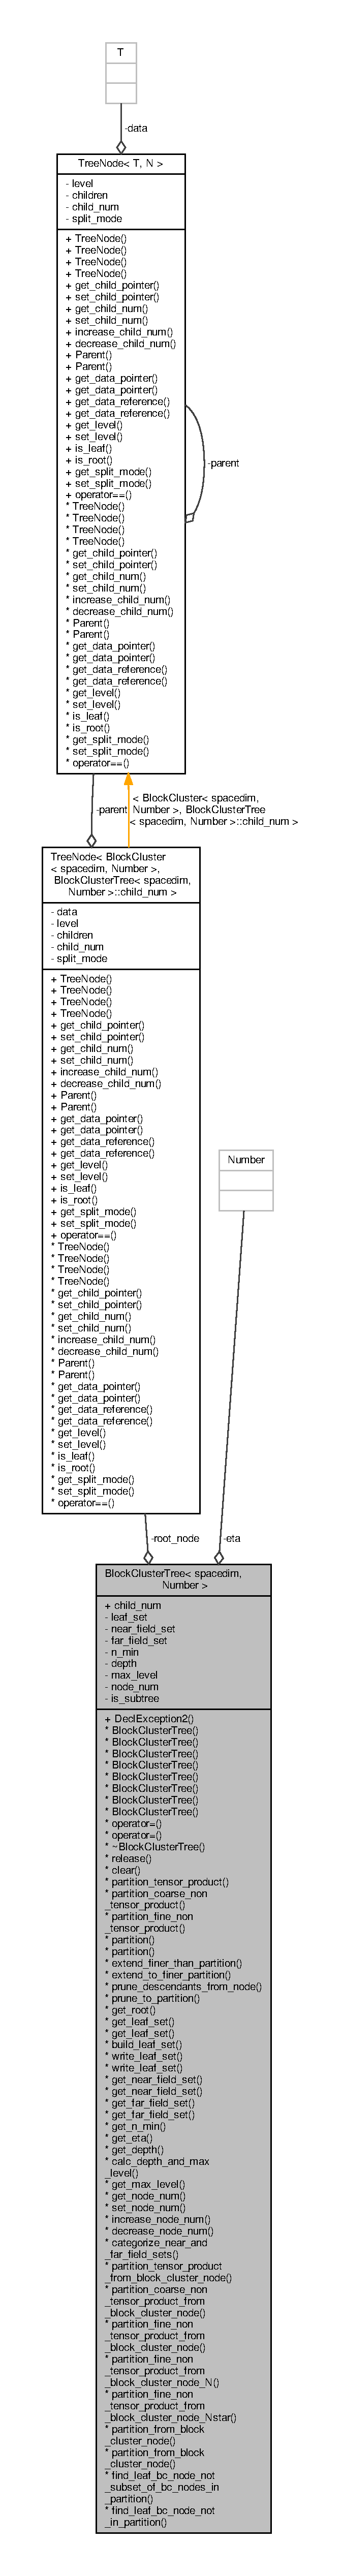
\includegraphics[height=550pt]{classBlockClusterTree__coll__graph}
\end{center}
\end{figure}
\subsection*{Public Types}
\begin{DoxyCompactItemize}
\item 
typedef \hyperlink{classTreeNode}{Tree\+Node}$<$ \hyperlink{classBlockCluster}{Block\+Cluster}$<$ spacedim, Number $>$, \hyperlink{classBlockClusterTree}{Block\+Cluster\+Tree}$<$ spacedim, Number $>$\+::\hyperlink{classBlockClusterTree_a000c439b578bcf4fa28b7f3edd6079e9}{child\+\_\+num} $>$ \hyperlink{classBlockClusterTree_a960c20eac27464dedd804261f185c61f}{node\+\_\+value\+\_\+type}
\item 
\mbox{\Hypertarget{classBlockClusterTree_a0fe6521e231371ee47687fc4ada1734a}\label{classBlockClusterTree_a0fe6521e231371ee47687fc4ada1734a}} 
typedef \hyperlink{classTreeNode}{Tree\+Node}$<$ \hyperlink{classBlockCluster}{Block\+Cluster}$<$ spacedim, Number $>$, \hyperlink{classBlockClusterTree}{Block\+Cluster\+Tree}$<$ spacedim, Number $>$\+::\hyperlink{classBlockClusterTree_a000c439b578bcf4fa28b7f3edd6079e9}{child\+\_\+num} $>$ $\ast$ {\bfseries node\+\_\+pointer\+\_\+type}
\item 
\mbox{\Hypertarget{classBlockClusterTree_ae009f8c6e64ac756770678366cf5e924}\label{classBlockClusterTree_ae009f8c6e64ac756770678366cf5e924}} 
typedef const \hyperlink{classTreeNode}{Tree\+Node}$<$ \hyperlink{classBlockCluster}{Block\+Cluster}$<$ spacedim, Number $>$, \hyperlink{classBlockClusterTree}{Block\+Cluster\+Tree}$<$ spacedim, Number $>$\+::\hyperlink{classBlockClusterTree_a000c439b578bcf4fa28b7f3edd6079e9}{child\+\_\+num} $>$ $\ast$ {\bfseries node\+\_\+const\+\_\+pointer\+\_\+type}
\item 
\mbox{\Hypertarget{classBlockClusterTree_acff2ef08707f864bce5da02be6f9f8a9}\label{classBlockClusterTree_acff2ef08707f864bce5da02be6f9f8a9}} 
typedef \hyperlink{classTreeNode}{Tree\+Node}$<$ \hyperlink{classBlockCluster}{Block\+Cluster}$<$ spacedim, Number $>$, \hyperlink{classBlockClusterTree}{Block\+Cluster\+Tree}$<$ spacedim, Number $>$\+::\hyperlink{classBlockClusterTree_a000c439b578bcf4fa28b7f3edd6079e9}{child\+\_\+num} $>$ \& {\bfseries node\+\_\+reference\+\_\+type}
\item 
\mbox{\Hypertarget{classBlockClusterTree_ac5dc9f60e63b4024045d1c0c41f92f5a}\label{classBlockClusterTree_ac5dc9f60e63b4024045d1c0c41f92f5a}} 
typedef const \hyperlink{classTreeNode}{Tree\+Node}$<$ \hyperlink{classBlockCluster}{Block\+Cluster}$<$ spacedim, Number $>$, \hyperlink{classBlockClusterTree}{Block\+Cluster\+Tree}$<$ spacedim, Number $>$\+::\hyperlink{classBlockClusterTree_a000c439b578bcf4fa28b7f3edd6079e9}{child\+\_\+num} $>$ \& {\bfseries node\+\_\+const\+\_\+reference\+\_\+type}
\item 
typedef \hyperlink{classBlockCluster}{Block\+Cluster}$<$ spacedim, Number $>$ \hyperlink{classBlockClusterTree_a4d03fe184a7f7838111b27cdae056a62}{data\+\_\+value\+\_\+type}
\item 
\mbox{\Hypertarget{classBlockClusterTree_a0480a48aa335fd1adeec9ffdc8086193}\label{classBlockClusterTree_a0480a48aa335fd1adeec9ffdc8086193}} 
typedef \hyperlink{classBlockCluster}{Block\+Cluster}$<$ spacedim, Number $>$ $\ast$ {\bfseries data\+\_\+pointer\+\_\+type}
\item 
\mbox{\Hypertarget{classBlockClusterTree_a179b726b207148de1b866d5c36915809}\label{classBlockClusterTree_a179b726b207148de1b866d5c36915809}} 
typedef const \hyperlink{classBlockCluster}{Block\+Cluster}$<$ spacedim, Number $>$ $\ast$ {\bfseries data\+\_\+const\+\_\+pointer\+\_\+type}
\item 
\mbox{\Hypertarget{classBlockClusterTree_a62869615d2fd6ec6bf58163e3b36bca1}\label{classBlockClusterTree_a62869615d2fd6ec6bf58163e3b36bca1}} 
typedef \hyperlink{classBlockCluster}{Block\+Cluster}$<$ spacedim, Number $>$ \& {\bfseries data\+\_\+reference\+\_\+type}
\item 
\mbox{\Hypertarget{classBlockClusterTree_a3ae82489506a1d2a0ff3cf0a4039b9f9}\label{classBlockClusterTree_a3ae82489506a1d2a0ff3cf0a4039b9f9}} 
typedef const \hyperlink{classBlockCluster}{Block\+Cluster}$<$ spacedim, Number $>$ \& {\bfseries data\+\_\+const\+\_\+reference\+\_\+type}
\end{DoxyCompactItemize}
\subsection*{Public Member Functions}
\begin{DoxyCompactItemize}
\item 
\mbox{\Hypertarget{classBlockClusterTree_a967049a8deecb49c36492ffdf64349cd}\label{classBlockClusterTree_a967049a8deecb49c36492ffdf64349cd}} 
{\bfseries Decl\+Exception2} (Exc\+Cluster\+Level\+Mismatch, unsigned int, unsigned int,$<$$<$ \char`\"{}The level of cluster tau \char`\"{}$<$$<$ arg1$<$$<$ \char`\"{} is different from that of cluster sigma\char`\"{}$<$$<$ arg2$<$$<$ \char`\"{} which is not allowed in a level preserving construction of a block cluster tree.\char`\"{})
\end{DoxyCompactItemize}
\subsection*{Static Public Attributes}
\begin{DoxyCompactItemize}
\item 
static const unsigned int \hyperlink{classBlockClusterTree_a000c439b578bcf4fa28b7f3edd6079e9}{child\+\_\+num} = 4
\end{DoxyCompactItemize}
\subsection*{Private Attributes}
\begin{DoxyCompactItemize}
\item 
\mbox{\Hypertarget{classBlockClusterTree_ac1111e02e99c25545857e6ce85c73fa0}\label{classBlockClusterTree_ac1111e02e99c25545857e6ce85c73fa0}} 
\hyperlink{classTreeNode}{node\+\_\+pointer\+\_\+type} {\bfseries root\+\_\+node}
\item 
\mbox{\Hypertarget{classBlockClusterTree_a4a070c8bebf3afb8eac8348be3cae226}\label{classBlockClusterTree_a4a070c8bebf3afb8eac8348be3cae226}} 
std\+::vector$<$ \hyperlink{classTreeNode}{node\+\_\+pointer\+\_\+type} $>$ {\bfseries leaf\+\_\+set}
\item 
\mbox{\Hypertarget{classBlockClusterTree_a91ff2520dacea664e08437b3bc54034a}\label{classBlockClusterTree_a91ff2520dacea664e08437b3bc54034a}} 
std\+::vector$<$ \hyperlink{classTreeNode}{node\+\_\+pointer\+\_\+type} $>$ {\bfseries near\+\_\+field\+\_\+set}
\item 
\mbox{\Hypertarget{classBlockClusterTree_afb80508e2eceac6545cdbac7310fcaa3}\label{classBlockClusterTree_afb80508e2eceac6545cdbac7310fcaa3}} 
std\+::vector$<$ \hyperlink{classTreeNode}{node\+\_\+pointer\+\_\+type} $>$ {\bfseries far\+\_\+field\+\_\+set}
\item 
\mbox{\Hypertarget{classBlockClusterTree_ab47a6ccabcf386897ea3fa4341827c25}\label{classBlockClusterTree_ab47a6ccabcf386897ea3fa4341827c25}} 
unsigned int {\bfseries n\+\_\+min}
\item 
\mbox{\Hypertarget{classBlockClusterTree_affa858180dc35e877eb64ab2afd1baef}\label{classBlockClusterTree_affa858180dc35e877eb64ab2afd1baef}} 
Number {\bfseries eta}
\item 
unsigned int \hyperlink{classBlockClusterTree_a77349ec9ccb36d45af3f176a93516897}{depth}
\item 
int \hyperlink{classBlockClusterTree_a9151f138713d01c53ac17f004c7e6b62}{max\+\_\+level}
\item 
unsigned int \hyperlink{classBlockClusterTree_a75757146cea0aa0e9271b760b1d76307}{node\+\_\+num}
\item 
bool \hyperlink{classBlockClusterTree_a8dc01af98989bb71246fa2cd4d7307da}{is\+\_\+subtree}
\end{DoxyCompactItemize}
\subsection*{Friends}
\begin{DoxyCompactItemize}
\item 
{\footnotesize template$<$int spacedim1, typename Number1 $>$ }\\std\+::ostream \& \hyperlink{classBlockClusterTree_a6ead7d49add78a2462eb039f00bf7f6a}{operator$<$$<$} (std\+::ostream \&out, const \hyperlink{classBlockClusterTree}{Block\+Cluster\+Tree}$<$ spacedim1, Number1 $>$ \&block\+\_\+cluster\+\_\+tree)
\item 
\mbox{\Hypertarget{classBlockClusterTree_a3f70501fa33bdb6761b998978b59f1b0}\label{classBlockClusterTree_a3f70501fa33bdb6761b998978b59f1b0}} 
{\footnotesize template$<$int spacedim1, typename Number1 $>$ }\\void {\bfseries split\+\_\+block\+\_\+cluster\+\_\+node} (\hyperlink{classTreeNode}{Tree\+Node}$<$ \hyperlink{classBlockCluster}{Block\+Cluster}$<$ spacedim1, Number1 $>$, \hyperlink{classBlockClusterTree}{Block\+Cluster\+Tree}$<$ spacedim1, Number1 $>$\+::\hyperlink{classBlockClusterTree_a000c439b578bcf4fa28b7f3edd6079e9}{child\+\_\+num} $>$ $\ast$bc\+\_\+node, \hyperlink{classBlockClusterTree}{Block\+Cluster\+Tree}$<$ spacedim1, Number1 $>$ \&bc\+\_\+tree, const \hyperlink{tree_8h_a922ca07db9633957939f697a65aff11d}{Tree\+Node\+Split\+Mode} split\+\_\+mode, const bool if\+\_\+add\+\_\+child\+\_\+nodes\+\_\+to\+\_\+leaf\+\_\+set)
\item 
\mbox{\Hypertarget{classBlockClusterTree_a75196d39c6db593dfdaa17f0f0cd8042}\label{classBlockClusterTree_a75196d39c6db593dfdaa17f0f0cd8042}} 
{\footnotesize template$<$int spacedim1, typename Number1 $>$ }\\bool {\bfseries prune\+\_\+to\+\_\+partition\+\_\+recursion} (\hyperlink{classBlockClusterTree}{Block\+Cluster\+Tree}$<$ spacedim1, Number1 $>$ \&bct, const std\+::vector$<$ \hyperlink{classTreeNode}{Tree\+Node}$<$ \hyperlink{classBlockCluster}{Block\+Cluster}$<$ spacedim1, Number1 $>$, \hyperlink{classBlockClusterTree}{Block\+Cluster\+Tree}$<$ spacedim1, Number1 $>$\+::\hyperlink{classBlockClusterTree_a000c439b578bcf4fa28b7f3edd6079e9}{child\+\_\+num} $>$ $\ast$$>$ \&\hyperlink{classBlockClusterTree_a3ca42421f732c20fc07bdf5d5ab94319}{partition}, \hyperlink{classTreeNode}{Tree\+Node}$<$ \hyperlink{classBlockCluster}{Block\+Cluster}$<$ spacedim1, Number1 $>$, \hyperlink{classBlockClusterTree}{Block\+Cluster\+Tree}$<$ spacedim1, Number1 $>$\+::\hyperlink{classBlockClusterTree_a000c439b578bcf4fa28b7f3edd6079e9}{child\+\_\+num} $>$ $\ast$bc\+\_\+node)
\item 
\mbox{\Hypertarget{classBlockClusterTree_a4be1a37fb4e8389d1035c532102aa20b}\label{classBlockClusterTree_a4be1a37fb4e8389d1035c532102aa20b}} 
{\footnotesize template$<$int spacedim1, typename Number1 $>$ }\\\hyperlink{classTreeNode}{Tree\+Node}$<$ \hyperlink{classBlockCluster}{Block\+Cluster}$<$ spacedim1, Number1 $>$, \hyperlink{classBlockClusterTree}{Block\+Cluster\+Tree}$<$ spacedim1, Number1 $>$\+::\hyperlink{classBlockClusterTree_a000c439b578bcf4fa28b7f3edd6079e9}{child\+\_\+num} $>$ $\ast$ {\bfseries find\+\_\+bc\+\_\+node\+\_\+in\+\_\+partition\+\_\+intersect\+\_\+current\+\_\+bc\+\_\+node} (\hyperlink{classTreeNode}{Tree\+Node}$<$ \hyperlink{classBlockCluster}{Block\+Cluster}$<$ spacedim1, Number1 $>$, \hyperlink{classBlockClusterTree}{Block\+Cluster\+Tree}$<$ spacedim1, Number1 $>$\+::\hyperlink{classBlockClusterTree_a000c439b578bcf4fa28b7f3edd6079e9}{child\+\_\+num} $>$ $\ast$current\+\_\+bc\+\_\+node, const std\+::vector$<$ \hyperlink{classTreeNode}{Tree\+Node}$<$ \hyperlink{classBlockCluster}{Block\+Cluster}$<$ spacedim1, Number1 $>$, \hyperlink{classBlockClusterTree}{Block\+Cluster\+Tree}$<$ spacedim1, Number1 $>$\+::\hyperlink{classBlockClusterTree_a000c439b578bcf4fa28b7f3edd6079e9}{child\+\_\+num} $>$ $\ast$$>$ \&\hyperlink{classBlockClusterTree_a3ca42421f732c20fc07bdf5d5ab94319}{partition})
\item 
\mbox{\Hypertarget{classBlockClusterTree_a1b5de5c860d62a2e28791afdbb2e2d72}\label{classBlockClusterTree_a1b5de5c860d62a2e28791afdbb2e2d72}} 
{\footnotesize template$<$int spacedim1, typename Number1 $>$ }\\\hyperlink{classTreeNode}{Tree\+Node}$<$ \hyperlink{classBlockCluster}{Block\+Cluster}$<$ spacedim1, Number1 $>$, \hyperlink{classBlockClusterTree}{Block\+Cluster\+Tree}$<$ spacedim1, Number1 $>$\+::\hyperlink{classBlockClusterTree_a000c439b578bcf4fa28b7f3edd6079e9}{child\+\_\+num} $>$ $\ast$ {\bfseries find\+\_\+bc\+\_\+node\+\_\+in\+\_\+partition\+\_\+proper\+\_\+subset\+\_\+of\+\_\+current\+\_\+bc\+\_\+node} (\hyperlink{classTreeNode}{Tree\+Node}$<$ \hyperlink{classBlockCluster}{Block\+Cluster}$<$ spacedim1, Number1 $>$, \hyperlink{classBlockClusterTree}{Block\+Cluster\+Tree}$<$ spacedim1, Number1 $>$\+::\hyperlink{classBlockClusterTree_a000c439b578bcf4fa28b7f3edd6079e9}{child\+\_\+num} $>$ $\ast$current\+\_\+bc\+\_\+node, const std\+::vector$<$ \hyperlink{classTreeNode}{Tree\+Node}$<$ \hyperlink{classBlockCluster}{Block\+Cluster}$<$ spacedim1, Number1 $>$, \hyperlink{classBlockClusterTree}{Block\+Cluster\+Tree}$<$ spacedim1, Number1 $>$\+::\hyperlink{classBlockClusterTree_a000c439b578bcf4fa28b7f3edd6079e9}{child\+\_\+num} $>$ $\ast$$>$ \&\hyperlink{classBlockClusterTree_a3ca42421f732c20fc07bdf5d5ab94319}{partition})
\end{DoxyCompactItemize}
\begin{DoxyCompactItemize}
\item 
\hyperlink{classBlockClusterTree_a20b1ec6a9e81c252b1994c5a99c44af4}{Block\+Cluster\+Tree} ()
\item 
\hyperlink{classBlockClusterTree_a61d415eda9bfffa9e0aa5492b461edab}{Block\+Cluster\+Tree} (const \hyperlink{classClusterTree}{Cluster\+Tree}$<$ spacedim, Number $>$ \&TI, const \hyperlink{classClusterTree}{Cluster\+Tree}$<$ spacedim, Number $>$ \&TJ, const unsigned int n\+\_\+min=0)
\item 
\hyperlink{classBlockClusterTree_a3073c9b5669e356c9c37ccd0a13ed8b3}{Block\+Cluster\+Tree} (typename \hyperlink{classClusterTree}{Cluster\+Tree}$<$ spacedim, Number $>$\+::\hyperlink{classTreeNode}{node\+\_\+pointer\+\_\+type} tau\+\_\+root\+\_\+node, typename \hyperlink{classClusterTree}{Cluster\+Tree}$<$ spacedim, Number $>$\+::\hyperlink{classTreeNode}{node\+\_\+pointer\+\_\+type} sigma\+\_\+root\+\_\+node, const unsigned int n\+\_\+min=1)
\item 
\hyperlink{classBlockClusterTree_ace6087e8fe7dc3d737ff6b4cd97070fc}{Block\+Cluster\+Tree} (\hyperlink{classTreeNode}{node\+\_\+pointer\+\_\+type} bc\+\_\+node, const unsigned int n\+\_\+min)
\item 
\hyperlink{classBlockClusterTree_a522ad51298f5b58b948e435a9e2d2a40}{Block\+Cluster\+Tree} (\hyperlink{classTreeNode}{node\+\_\+pointer\+\_\+type} bc\+\_\+node, const Number eta, const unsigned int n\+\_\+min)
\item 
\hyperlink{classBlockClusterTree_aefb93288ece0e153eb5843d1df21a2a6}{Block\+Cluster\+Tree} (const \hyperlink{classClusterTree}{Cluster\+Tree}$<$ spacedim, Number $>$ \&TI, const \hyperlink{classClusterTree}{Cluster\+Tree}$<$ spacedim, Number $>$ \&TJ, const Number eta, const unsigned int n\+\_\+min)
\item 
\hyperlink{classBlockClusterTree_a1c31aecfd91383f8b96601fd2b63dd62}{Block\+Cluster\+Tree} (const \hyperlink{classBlockClusterTree}{Block\+Cluster\+Tree}$<$ spacedim, Number $>$ \&bct)
\item 
\hyperlink{classBlockClusterTree_ae3bb67cdcb7868237063c8003d4079ab}{Block\+Cluster\+Tree} (\hyperlink{classBlockClusterTree}{Block\+Cluster\+Tree}$<$ spacedim, Number $>$ \&\&bct)
\item 
\hyperlink{classBlockClusterTree}{Block\+Cluster\+Tree}$<$ spacedim, Number $>$ \& \hyperlink{classBlockClusterTree_a85553cc442e419b8d707720312118328}{operator=} (const \hyperlink{classBlockClusterTree}{Block\+Cluster\+Tree}$<$ spacedim, Number $>$ \&bct)
\item 
\hyperlink{classBlockClusterTree}{Block\+Cluster\+Tree}$<$ spacedim, Number $>$ \& \hyperlink{classBlockClusterTree_aa635be81dfabed3ba455a17de3b65c2e}{operator=} (\hyperlink{classBlockClusterTree}{Block\+Cluster\+Tree}$<$ spacedim, Number $>$ \&\&bct)
\item 
\hyperlink{classBlockClusterTree_a43b969867200b06f3416647c3e4f9f61}{$\sim$\+Block\+Cluster\+Tree} ()
\item 
void \hyperlink{classBlockClusterTree_a0415fe94fd480bbb985a45dc691e2bed}{release} ()
\item 
void \hyperlink{classBlockClusterTree_ab4227d666cd2872fbbfb4eec69e66313}{clear} ()
\item 
void \hyperlink{classBlockClusterTree_ab10f54639969bc4aacd6aa27cf315610}{partition\+\_\+tensor\+\_\+product} ()
\item 
void \hyperlink{classBlockClusterTree_a0e40b3884535eae57d00c078ec782459}{partition\+\_\+coarse\+\_\+non\+\_\+tensor\+\_\+product} ()
\item 
void \hyperlink{classBlockClusterTree_ac6d23af20c52c7b32eb080bd54556206}{partition\+\_\+fine\+\_\+non\+\_\+tensor\+\_\+product} ()
\item 
void \hyperlink{classBlockClusterTree_a3ca42421f732c20fc07bdf5d5ab94319}{partition} (const std\+::vector$<$ Point$<$ spacedim $>$$>$ \&all\+\_\+support\+\_\+points)
\item 
void \hyperlink{classBlockClusterTree_a075983197c805c6451aa00502dc30e76}{partition} (const std\+::vector$<$ Point$<$ spacedim $>$$>$ \&all\+\_\+support\+\_\+points, const std\+::vector$<$ Number $>$ \&cell\+\_\+size\+\_\+at\+\_\+dofs)
\item 
bool \hyperlink{classBlockClusterTree_a3c4a4da89b964559cc02ecbf13ad4a4b}{extend\+\_\+finer\+\_\+than\+\_\+partition} (const std\+::vector$<$ \hyperlink{classTreeNode}{node\+\_\+pointer\+\_\+type} $>$ \&\hyperlink{classBlockClusterTree_a3ca42421f732c20fc07bdf5d5ab94319}{partition})
\item 
bool \hyperlink{classBlockClusterTree_adfe18d32a3c05a9209a5cdc9270b47d7}{extend\+\_\+to\+\_\+finer\+\_\+partition} (const std\+::vector$<$ \hyperlink{classTreeNode}{node\+\_\+pointer\+\_\+type} $>$ \&\hyperlink{classBlockClusterTree_a3ca42421f732c20fc07bdf5d5ab94319}{partition})
\item 
bool \hyperlink{classBlockClusterTree_a6fd771b68a4c7195151f6dc02e8ec7e9}{prune\+\_\+descendants\+\_\+from\+\_\+node} (\hyperlink{classTreeNode}{node\+\_\+pointer\+\_\+type} bc\+\_\+node)
\item 
bool \hyperlink{classBlockClusterTree_af1663a109b6fd5c67c85e9bb88a54a13}{prune\+\_\+to\+\_\+partition} (const std\+::vector$<$ \hyperlink{classTreeNode}{node\+\_\+pointer\+\_\+type} $>$ \&\hyperlink{classBlockClusterTree_a3ca42421f732c20fc07bdf5d5ab94319}{partition}, const bool is\+\_\+partition\+\_\+in\+\_\+bct)
\item 
\hyperlink{classTreeNode}{node\+\_\+pointer\+\_\+type} \hyperlink{classBlockClusterTree_a4a4f3b893380d1d7f53b772589a847d2}{get\+\_\+root} () const
\item 
std\+::vector$<$ \hyperlink{classTreeNode}{node\+\_\+pointer\+\_\+type} $>$ \& \hyperlink{classBlockClusterTree_a162b396d814b420f96289425529852e9}{get\+\_\+leaf\+\_\+set} ()
\item 
const std\+::vector$<$ \hyperlink{classTreeNode}{node\+\_\+pointer\+\_\+type} $>$ \& \hyperlink{classBlockClusterTree_a38c3d1ad3aa983ea1d0b711914664b4c}{get\+\_\+leaf\+\_\+set} () const
\item 
void \hyperlink{classBlockClusterTree_a1b3396fbedf6ec07cce9c23a62b2c30b}{build\+\_\+leaf\+\_\+set} ()
\item 
void \hyperlink{classBlockClusterTree_aef01b51b0530536bc5481492d4719375}{write\+\_\+leaf\+\_\+set} (std\+::ostream \&out) const
\item 
{\footnotesize template$<$typename Number1  = double$>$ }\\void \hyperlink{classBlockClusterTree_a652b1c53dff2794e2f18343bf3988e19}{write\+\_\+leaf\+\_\+set} (std\+::ostream \&out, const \hyperlink{classLAPACKFullMatrixExt}{L\+A\+P\+A\+C\+K\+Full\+Matrix\+Ext}$<$ Number1 $>$ \&matrix, const Number1 singular\+\_\+value\+\_\+threshold=0.) const
\item 
std\+::vector$<$ \hyperlink{classTreeNode}{node\+\_\+pointer\+\_\+type} $>$ \& \hyperlink{classBlockClusterTree_a82f61b31f1e9cf869831fa4c8232df81}{get\+\_\+near\+\_\+field\+\_\+set} ()
\item 
const std\+::vector$<$ \hyperlink{classTreeNode}{node\+\_\+pointer\+\_\+type} $>$ \& \hyperlink{classBlockClusterTree_a6ac71437177d14012c12f7b4f354cdd1}{get\+\_\+near\+\_\+field\+\_\+set} () const
\item 
std\+::vector$<$ \hyperlink{classTreeNode}{node\+\_\+pointer\+\_\+type} $>$ \& \hyperlink{classBlockClusterTree_a2980726dc3789773b5cd3c04df5e69a3}{get\+\_\+far\+\_\+field\+\_\+set} ()
\item 
const std\+::vector$<$ \hyperlink{classTreeNode}{node\+\_\+pointer\+\_\+type} $>$ \& \hyperlink{classBlockClusterTree_a93763855c84100e1a9da3080737295f4}{get\+\_\+far\+\_\+field\+\_\+set} () const
\item 
unsigned int \hyperlink{classBlockClusterTree_ab00acda5e8fd4c3e381637d8d9322923}{get\+\_\+n\+\_\+min} () const
\item 
Number \hyperlink{classBlockClusterTree_a312d01ddb6cf5560d84abf7d254fa2c3}{get\+\_\+eta} () const
\item 
unsigned int \hyperlink{classBlockClusterTree_ab6c57acfcc5dfbbef04f028e6b9c749d}{get\+\_\+depth} () const
\item 
void \hyperlink{classBlockClusterTree_a7f9dbea25751771830c72d09efacacb2}{calc\+\_\+depth\+\_\+and\+\_\+max\+\_\+level} ()
\item 
int \hyperlink{classBlockClusterTree_a404693ef7dfdbc383705c38105c75e14}{get\+\_\+max\+\_\+level} () const
\item 
unsigned int \hyperlink{classBlockClusterTree_a042e040d2f6dfcbbfd70b43b8967c6f6}{get\+\_\+node\+\_\+num} () const
\item 
void \hyperlink{classBlockClusterTree_a02be4a882acca918386ad024769925bc}{set\+\_\+node\+\_\+num} (unsigned int \hyperlink{classBlockClusterTree_a75757146cea0aa0e9271b760b1d76307}{node\+\_\+num})
\item 
unsigned int \hyperlink{classBlockClusterTree_aec9920e5b215fbfe2aa9f54980d3b30a}{increase\+\_\+node\+\_\+num} (unsigned int increased\+\_\+node\+\_\+num=1)
\item 
unsigned int \hyperlink{classBlockClusterTree_ae0e55e3ac56bffa31f251d4f07ae7e51}{decrease\+\_\+node\+\_\+num} (unsigned int decreased\+\_\+node\+\_\+num=1)
\item 
void \hyperlink{classBlockClusterTree_a286bd48cc863cbba7c9ad53b6bdb12ca}{categorize\+\_\+near\+\_\+and\+\_\+far\+\_\+field\+\_\+sets} ()
\item 
void \hyperlink{classBlockClusterTree_ae77f8167ce49871f5751b8dcf8c93153}{partition\+\_\+tensor\+\_\+product\+\_\+from\+\_\+block\+\_\+cluster\+\_\+node} (\hyperlink{classTreeNode}{node\+\_\+pointer\+\_\+type} current\+\_\+block\+\_\+cluster\+\_\+node, std\+::vector$<$ \hyperlink{classTreeNode}{node\+\_\+pointer\+\_\+type} $>$ \&leaf\+\_\+set\+\_\+wrt\+\_\+current\+\_\+node)
\item 
void \hyperlink{classBlockClusterTree_a61b6c204f3f1d5ff7c71a07b26ca9d09}{partition\+\_\+coarse\+\_\+non\+\_\+tensor\+\_\+product\+\_\+from\+\_\+block\+\_\+cluster\+\_\+node} (\hyperlink{classTreeNode}{node\+\_\+pointer\+\_\+type} current\+\_\+block\+\_\+cluster\+\_\+node, std\+::vector$<$ \hyperlink{classTreeNode}{node\+\_\+pointer\+\_\+type} $>$ \&leaf\+\_\+set\+\_\+wrt\+\_\+current\+\_\+node)
\item 
void \hyperlink{classBlockClusterTree_aa6354696477c8cae61d362b5ec707034}{partition\+\_\+fine\+\_\+non\+\_\+tensor\+\_\+product\+\_\+from\+\_\+block\+\_\+cluster\+\_\+node} (\hyperlink{classTreeNode}{node\+\_\+pointer\+\_\+type} current\+\_\+block\+\_\+cluster\+\_\+node, std\+::vector$<$ \hyperlink{classTreeNode}{node\+\_\+pointer\+\_\+type} $>$ \&leaf\+\_\+set\+\_\+wrt\+\_\+current\+\_\+node)
\item 
void \hyperlink{classBlockClusterTree_aafad0fae48bf7c462e8e943b76893fc0}{partition\+\_\+fine\+\_\+non\+\_\+tensor\+\_\+product\+\_\+from\+\_\+block\+\_\+cluster\+\_\+node\+\_\+N} (\hyperlink{classTreeNode}{node\+\_\+pointer\+\_\+type} current\+\_\+block\+\_\+cluster\+\_\+node, std\+::vector$<$ \hyperlink{classTreeNode}{node\+\_\+pointer\+\_\+type} $>$ \&leaf\+\_\+set\+\_\+wrt\+\_\+current\+\_\+node)
\item 
void \hyperlink{classBlockClusterTree_afdeb6723e01b5eaf11281e2c1c1cf566}{partition\+\_\+fine\+\_\+non\+\_\+tensor\+\_\+product\+\_\+from\+\_\+block\+\_\+cluster\+\_\+node\+\_\+\+Nstar} (\hyperlink{classTreeNode}{node\+\_\+pointer\+\_\+type} current\+\_\+block\+\_\+cluster\+\_\+node, std\+::vector$<$ \hyperlink{classTreeNode}{node\+\_\+pointer\+\_\+type} $>$ \&leaf\+\_\+set\+\_\+wrt\+\_\+current\+\_\+node)
\item 
void \hyperlink{classBlockClusterTree_ad11fb277e43c33f2a399dc6b1c14b998}{partition\+\_\+from\+\_\+block\+\_\+cluster\+\_\+node} (\hyperlink{classTreeNode}{node\+\_\+pointer\+\_\+type} current\+\_\+block\+\_\+cluster\+\_\+node, const std\+::vector$<$ Point$<$ spacedim $>$$>$ \&all\+\_\+support\+\_\+points, std\+::vector$<$ \hyperlink{classTreeNode}{node\+\_\+pointer\+\_\+type} $>$ \&leaf\+\_\+set\+\_\+wrt\+\_\+current\+\_\+node)
\item 
void \hyperlink{classBlockClusterTree_a425583a70d63ddbf9341a31b736bd0fe}{partition\+\_\+from\+\_\+block\+\_\+cluster\+\_\+node} (\hyperlink{classTreeNode}{node\+\_\+pointer\+\_\+type} current\+\_\+block\+\_\+cluster\+\_\+node, const std\+::vector$<$ Point$<$ spacedim $>$$>$ \&all\+\_\+support\+\_\+points, const std\+::vector$<$ Number $>$ \&cell\+\_\+size\+\_\+at\+\_\+dofs, std\+::vector$<$ \hyperlink{classTreeNode}{node\+\_\+pointer\+\_\+type} $>$ \&leaf\+\_\+set\+\_\+wrt\+\_\+current\+\_\+node)
\item 
\hyperlink{classTreeNode}{node\+\_\+pointer\+\_\+type} \hyperlink{classBlockClusterTree_a97a99684ebd9ed470a79e56b73374068}{find\+\_\+leaf\+\_\+bc\+\_\+node\+\_\+not\+\_\+subset\+\_\+of\+\_\+bc\+\_\+nodes\+\_\+in\+\_\+partition} (const std\+::vector$<$ \hyperlink{classTreeNode}{node\+\_\+pointer\+\_\+type} $>$ \&\hyperlink{classBlockClusterTree_a3ca42421f732c20fc07bdf5d5ab94319}{partition}, typename std\+::vector$<$ \hyperlink{classTreeNode}{node\+\_\+pointer\+\_\+type} $>$\+::const\+\_\+iterator \&it\+\_\+for\+\_\+desired\+\_\+bc\+\_\+node) const
\item 
\hyperlink{classTreeNode}{node\+\_\+pointer\+\_\+type} \hyperlink{classBlockClusterTree_a4782e1e817b6e6265bff43baf2b1dbaa}{find\+\_\+leaf\+\_\+bc\+\_\+node\+\_\+not\+\_\+in\+\_\+partition} (const std\+::vector$<$ \hyperlink{classTreeNode}{node\+\_\+pointer\+\_\+type} $>$ \&\hyperlink{classBlockClusterTree_a3ca42421f732c20fc07bdf5d5ab94319}{partition}, typename std\+::vector$<$ \hyperlink{classTreeNode}{node\+\_\+pointer\+\_\+type} $>$\+::const\+\_\+iterator \&it\+\_\+for\+\_\+desired\+\_\+bc\+\_\+node) const
\end{DoxyCompactItemize}


\subsection{Detailed Description}
\subsubsection*{template$<$int spacedim, typename Number = double$>$\newline
class Block\+Cluster\+Tree$<$ spacedim, Number $>$}

Class for block cluster tree. 

A block cluster tree is a quad-\/tree which holds a hierarchy of doubly linked nodes with the type \hyperlink{classTreeNode}{Tree\+Node}. Because a node in the block cluster tree has four children, the template argument {\ttfamily T} required by {\ttfamily \hyperlink{classTreeNode}{Tree\+Node}} should be 4. 

\subsection{Member Typedef Documentation}
\mbox{\Hypertarget{classBlockClusterTree_a4d03fe184a7f7838111b27cdae056a62}\label{classBlockClusterTree_a4d03fe184a7f7838111b27cdae056a62}} 
\index{Block\+Cluster\+Tree@{Block\+Cluster\+Tree}!data\+\_\+value\+\_\+type@{data\+\_\+value\+\_\+type}}
\index{data\+\_\+value\+\_\+type@{data\+\_\+value\+\_\+type}!Block\+Cluster\+Tree@{Block\+Cluster\+Tree}}
\subsubsection{\texorpdfstring{data\+\_\+value\+\_\+type}{data\_value\_type}}
{\footnotesize\ttfamily template$<$int spacedim, typename Number = double$>$ \\
typedef \hyperlink{classBlockCluster}{Block\+Cluster}$<$spacedim, Number$>$ \hyperlink{classBlockClusterTree}{Block\+Cluster\+Tree}$<$ spacedim, Number $>$\+::\hyperlink{classBlockClusterTree_a4d03fe184a7f7838111b27cdae056a62}{data\+\_\+value\+\_\+type}}

Data type of the data held by a tree node. \mbox{\Hypertarget{classBlockClusterTree_a960c20eac27464dedd804261f185c61f}\label{classBlockClusterTree_a960c20eac27464dedd804261f185c61f}} 
\index{Block\+Cluster\+Tree@{Block\+Cluster\+Tree}!node\+\_\+value\+\_\+type@{node\+\_\+value\+\_\+type}}
\index{node\+\_\+value\+\_\+type@{node\+\_\+value\+\_\+type}!Block\+Cluster\+Tree@{Block\+Cluster\+Tree}}
\subsubsection{\texorpdfstring{node\+\_\+value\+\_\+type}{node\_value\_type}}
{\footnotesize\ttfamily template$<$int spacedim, typename Number = double$>$ \\
typedef \hyperlink{classTreeNode}{Tree\+Node}$<$\hyperlink{classBlockCluster}{Block\+Cluster}$<$spacedim, Number$>$, \hyperlink{classBlockClusterTree}{Block\+Cluster\+Tree}$<$spacedim, Number$>$\+::\hyperlink{classBlockClusterTree_a000c439b578bcf4fa28b7f3edd6079e9}{child\+\_\+num}$>$ \hyperlink{classBlockClusterTree}{Block\+Cluster\+Tree}$<$ spacedim, Number $>$\+::\hyperlink{classBlockClusterTree_a960c20eac27464dedd804261f185c61f}{node\+\_\+value\+\_\+type}}

Data type of the tree node. 

\subsection{Constructor \& Destructor Documentation}
\mbox{\Hypertarget{classBlockClusterTree_a20b1ec6a9e81c252b1994c5a99c44af4}\label{classBlockClusterTree_a20b1ec6a9e81c252b1994c5a99c44af4}} 
\index{Block\+Cluster\+Tree@{Block\+Cluster\+Tree}!Block\+Cluster\+Tree@{Block\+Cluster\+Tree}}
\index{Block\+Cluster\+Tree@{Block\+Cluster\+Tree}!Block\+Cluster\+Tree@{Block\+Cluster\+Tree}}
\subsubsection{\texorpdfstring{Block\+Cluster\+Tree()}{BlockClusterTree()}\hspace{0.1cm}{\footnotesize\ttfamily [1/8]}}
{\footnotesize\ttfamily template$<$int spacedim, typename Number $>$ \\
\hyperlink{classBlockClusterTree}{Block\+Cluster\+Tree}$<$ spacedim, Number $>$\+::\hyperlink{classBlockClusterTree}{Block\+Cluster\+Tree} (\begin{DoxyParamCaption}{ }\end{DoxyParamCaption})}

Default constructor, which initializes an empty quad-\/tree. \mbox{\Hypertarget{classBlockClusterTree_a61d415eda9bfffa9e0aa5492b461edab}\label{classBlockClusterTree_a61d415eda9bfffa9e0aa5492b461edab}} 
\index{Block\+Cluster\+Tree@{Block\+Cluster\+Tree}!Block\+Cluster\+Tree@{Block\+Cluster\+Tree}}
\index{Block\+Cluster\+Tree@{Block\+Cluster\+Tree}!Block\+Cluster\+Tree@{Block\+Cluster\+Tree}}
\subsubsection{\texorpdfstring{Block\+Cluster\+Tree()}{BlockClusterTree()}\hspace{0.1cm}{\footnotesize\ttfamily [2/8]}}
{\footnotesize\ttfamily template$<$int spacedim, typename Number$>$ \\
\hyperlink{classBlockClusterTree}{Block\+Cluster\+Tree}$<$ spacedim, Number $>$\+::\hyperlink{classBlockClusterTree}{Block\+Cluster\+Tree} (\begin{DoxyParamCaption}\item[{const \hyperlink{classClusterTree}{Cluster\+Tree}$<$ spacedim, Number $>$ \&}]{TI,  }\item[{const \hyperlink{classClusterTree}{Cluster\+Tree}$<$ spacedim, Number $>$ \&}]{TJ,  }\item[{const unsigned int}]{n\+\_\+min = {\ttfamily 0} }\end{DoxyParamCaption})}

Construct from two cluster trees built from pure cardinality based partition, which has no admissibility condition.

After construction, there is only one node in the block cluster tree, i.\+e. tree hierarchy is not built.


\begin{DoxyParams}{Parameters}
{\em TI} & \\
\hline
{\em TJ} & \\
\hline
{\em n\+\_\+min} & \\
\hline
\end{DoxyParams}
\mbox{\Hypertarget{classBlockClusterTree_a3073c9b5669e356c9c37ccd0a13ed8b3}\label{classBlockClusterTree_a3073c9b5669e356c9c37ccd0a13ed8b3}} 
\index{Block\+Cluster\+Tree@{Block\+Cluster\+Tree}!Block\+Cluster\+Tree@{Block\+Cluster\+Tree}}
\index{Block\+Cluster\+Tree@{Block\+Cluster\+Tree}!Block\+Cluster\+Tree@{Block\+Cluster\+Tree}}
\subsubsection{\texorpdfstring{Block\+Cluster\+Tree()}{BlockClusterTree()}\hspace{0.1cm}{\footnotesize\ttfamily [3/8]}}
{\footnotesize\ttfamily template$<$int spacedim, typename Number$>$ \\
\hyperlink{classBlockClusterTree}{Block\+Cluster\+Tree}$<$ spacedim, Number $>$\+::\hyperlink{classBlockClusterTree}{Block\+Cluster\+Tree} (\begin{DoxyParamCaption}\item[{typename \hyperlink{classClusterTree}{Cluster\+Tree}$<$ spacedim, Number $>$\+::\hyperlink{classTreeNode}{node\+\_\+pointer\+\_\+type}}]{tau\+\_\+root\+\_\+node,  }\item[{typename \hyperlink{classClusterTree}{Cluster\+Tree}$<$ spacedim, Number $>$\+::\hyperlink{classTreeNode}{node\+\_\+pointer\+\_\+type}}]{sigma\+\_\+root\+\_\+node,  }\item[{const unsigned int}]{n\+\_\+min = {\ttfamily 1} }\end{DoxyParamCaption})}

Construct from two cluster nodes, whose Cartesian product is the root node of the block cluster tree.

After construction, there is only one node in the block cluster tree, i.\+e. tree hierarchy is not built.


\begin{DoxyParams}{Parameters}
{\em tau\+\_\+root\+\_\+node} & \\
\hline
{\em sigma\+\_\+root\+\_\+node} & \\
\hline
\end{DoxyParams}
\mbox{\Hypertarget{classBlockClusterTree_ace6087e8fe7dc3d737ff6b4cd97070fc}\label{classBlockClusterTree_ace6087e8fe7dc3d737ff6b4cd97070fc}} 
\index{Block\+Cluster\+Tree@{Block\+Cluster\+Tree}!Block\+Cluster\+Tree@{Block\+Cluster\+Tree}}
\index{Block\+Cluster\+Tree@{Block\+Cluster\+Tree}!Block\+Cluster\+Tree@{Block\+Cluster\+Tree}}
\subsubsection{\texorpdfstring{Block\+Cluster\+Tree()}{BlockClusterTree()}\hspace{0.1cm}{\footnotesize\ttfamily [4/8]}}
{\footnotesize\ttfamily template$<$int spacedim, typename Number$>$ \\
\hyperlink{classBlockClusterTree}{Block\+Cluster\+Tree}$<$ spacedim, Number $>$\+::\hyperlink{classBlockClusterTree}{Block\+Cluster\+Tree} (\begin{DoxyParamCaption}\item[{\hyperlink{classTreeNode}{node\+\_\+pointer\+\_\+type}}]{bc\+\_\+node,  }\item[{const unsigned int}]{n\+\_\+min }\end{DoxyParamCaption})}

Construct a block cluster subtree by initializing from a block cluster node.

The constructed block cluster subtree simply takes over an existing block cluster node in a block cluster tree which has been built before.


\begin{DoxyParams}{Parameters}
{\em bc\+\_\+node} & \\
\hline
{\em n\+\_\+min} & \\
\hline
\end{DoxyParams}
\mbox{\Hypertarget{classBlockClusterTree_a522ad51298f5b58b948e435a9e2d2a40}\label{classBlockClusterTree_a522ad51298f5b58b948e435a9e2d2a40}} 
\index{Block\+Cluster\+Tree@{Block\+Cluster\+Tree}!Block\+Cluster\+Tree@{Block\+Cluster\+Tree}}
\index{Block\+Cluster\+Tree@{Block\+Cluster\+Tree}!Block\+Cluster\+Tree@{Block\+Cluster\+Tree}}
\subsubsection{\texorpdfstring{Block\+Cluster\+Tree()}{BlockClusterTree()}\hspace{0.1cm}{\footnotesize\ttfamily [5/8]}}
{\footnotesize\ttfamily template$<$int spacedim, typename Number$>$ \\
\hyperlink{classBlockClusterTree}{Block\+Cluster\+Tree}$<$ spacedim, Number $>$\+::\hyperlink{classBlockClusterTree}{Block\+Cluster\+Tree} (\begin{DoxyParamCaption}\item[{\hyperlink{classTreeNode}{node\+\_\+pointer\+\_\+type}}]{bc\+\_\+node,  }\item[{const Number}]{eta,  }\item[{const unsigned int}]{n\+\_\+min }\end{DoxyParamCaption})}

Construct a block cluster subtree by initializing from a block cluster node. This version has the admissibility condition.

The constructed block cluster subtree simply takes over an existing block cluster node in a block cluster tree which has been built before.


\begin{DoxyParams}{Parameters}
{\em bc\+\_\+node} & \\
\hline
\end{DoxyParams}
\mbox{\Hypertarget{classBlockClusterTree_aefb93288ece0e153eb5843d1df21a2a6}\label{classBlockClusterTree_aefb93288ece0e153eb5843d1df21a2a6}} 
\index{Block\+Cluster\+Tree@{Block\+Cluster\+Tree}!Block\+Cluster\+Tree@{Block\+Cluster\+Tree}}
\index{Block\+Cluster\+Tree@{Block\+Cluster\+Tree}!Block\+Cluster\+Tree@{Block\+Cluster\+Tree}}
\subsubsection{\texorpdfstring{Block\+Cluster\+Tree()}{BlockClusterTree()}\hspace{0.1cm}{\footnotesize\ttfamily [6/8]}}
{\footnotesize\ttfamily template$<$int spacedim, typename Number$>$ \\
\hyperlink{classBlockClusterTree}{Block\+Cluster\+Tree}$<$ spacedim, Number $>$\+::\hyperlink{classBlockClusterTree}{Block\+Cluster\+Tree} (\begin{DoxyParamCaption}\item[{const \hyperlink{classClusterTree}{Cluster\+Tree}$<$ spacedim, Number $>$ \&}]{TI,  }\item[{const \hyperlink{classClusterTree}{Cluster\+Tree}$<$ spacedim, Number $>$ \&}]{TJ,  }\item[{const Number}]{eta,  }\item[{const unsigned int}]{n\+\_\+min }\end{DoxyParamCaption})}

Construct from two cluster trees and admissibility condition.

The Cartesian product of the two clusters in the root nodes of $T(I)$ and $T(J)$ becomes the data in the root node of the block cluster tree.

After construction, there is only one node in the block cluster tree, i.\+e. tree hierarchy is not built. \mbox{\Hypertarget{classBlockClusterTree_a1c31aecfd91383f8b96601fd2b63dd62}\label{classBlockClusterTree_a1c31aecfd91383f8b96601fd2b63dd62}} 
\index{Block\+Cluster\+Tree@{Block\+Cluster\+Tree}!Block\+Cluster\+Tree@{Block\+Cluster\+Tree}}
\index{Block\+Cluster\+Tree@{Block\+Cluster\+Tree}!Block\+Cluster\+Tree@{Block\+Cluster\+Tree}}
\subsubsection{\texorpdfstring{Block\+Cluster\+Tree()}{BlockClusterTree()}\hspace{0.1cm}{\footnotesize\ttfamily [7/8]}}
{\footnotesize\ttfamily template$<$int spacedim, typename Number$>$ \\
\hyperlink{classBlockClusterTree}{Block\+Cluster\+Tree}$<$ spacedim, Number $>$\+::\hyperlink{classBlockClusterTree}{Block\+Cluster\+Tree} (\begin{DoxyParamCaption}\item[{const \hyperlink{classBlockClusterTree}{Block\+Cluster\+Tree}$<$ spacedim, Number $>$ \&}]{bct }\end{DoxyParamCaption})}

Copy constructor for {\ttfamily \hyperlink{classBlockClusterTree}{Block\+Cluster\+Tree}}, which realizes deep copy internally.


\begin{DoxyDescription}
\item[Note ]Because this is deep copy, the constructed block cluster tree is a new tree but never a subtree of an existing block cluster tree. Hence, the data field {\ttfamily is\+\_\+subtree} is set to {\ttfamily false}. 
\end{DoxyDescription}


\begin{DoxyParams}{Parameters}
{\em bct} & \\
\hline
\end{DoxyParams}
\mbox{\Hypertarget{classBlockClusterTree_ae3bb67cdcb7868237063c8003d4079ab}\label{classBlockClusterTree_ae3bb67cdcb7868237063c8003d4079ab}} 
\index{Block\+Cluster\+Tree@{Block\+Cluster\+Tree}!Block\+Cluster\+Tree@{Block\+Cluster\+Tree}}
\index{Block\+Cluster\+Tree@{Block\+Cluster\+Tree}!Block\+Cluster\+Tree@{Block\+Cluster\+Tree}}
\subsubsection{\texorpdfstring{Block\+Cluster\+Tree()}{BlockClusterTree()}\hspace{0.1cm}{\footnotesize\ttfamily [8/8]}}
{\footnotesize\ttfamily template$<$int spacedim, typename Number$>$ \\
\hyperlink{classBlockClusterTree}{Block\+Cluster\+Tree}$<$ spacedim, Number $>$\+::\hyperlink{classBlockClusterTree}{Block\+Cluster\+Tree} (\begin{DoxyParamCaption}\item[{\hyperlink{classBlockClusterTree}{Block\+Cluster\+Tree}$<$ spacedim, Number $>$ \&\&}]{bct }\end{DoxyParamCaption})}

Copy constructor via shallow copy.


\begin{DoxyDescription}
\item[Note ]The data members of the input {\ttfamily bct} must be cleared before exiting this constructor. Otherwise, when {\ttfamily bct} is out of its range, the data associated with the current block cluster tree will also be destroyed, which is undesired. 
\end{DoxyDescription}


\begin{DoxyParams}{Parameters}
{\em bct} & \\
\hline
\end{DoxyParams}
\begin{DoxyReturn}{Returns}

\end{DoxyReturn}
\mbox{\Hypertarget{classBlockClusterTree_a43b969867200b06f3416647c3e4f9f61}\label{classBlockClusterTree_a43b969867200b06f3416647c3e4f9f61}} 
\index{Block\+Cluster\+Tree@{Block\+Cluster\+Tree}!````~Block\+Cluster\+Tree@{$\sim$\+Block\+Cluster\+Tree}}
\index{````~Block\+Cluster\+Tree@{$\sim$\+Block\+Cluster\+Tree}!Block\+Cluster\+Tree@{Block\+Cluster\+Tree}}
\subsubsection{\texorpdfstring{$\sim$\+Block\+Cluster\+Tree()}{~BlockClusterTree()}}
{\footnotesize\ttfamily template$<$int spacedim, typename Number $>$ \\
\hyperlink{classBlockClusterTree}{Block\+Cluster\+Tree}$<$ spacedim, Number $>$\+::$\sim$\hyperlink{classBlockClusterTree}{Block\+Cluster\+Tree} (\begin{DoxyParamCaption}{ }\end{DoxyParamCaption})}

Destructor which recursively destroys every node in the block cluster tree. 

\subsection{Member Function Documentation}
\mbox{\Hypertarget{classBlockClusterTree_a1b3396fbedf6ec07cce9c23a62b2c30b}\label{classBlockClusterTree_a1b3396fbedf6ec07cce9c23a62b2c30b}} 
\index{Block\+Cluster\+Tree@{Block\+Cluster\+Tree}!build\+\_\+leaf\+\_\+set@{build\+\_\+leaf\+\_\+set}}
\index{build\+\_\+leaf\+\_\+set@{build\+\_\+leaf\+\_\+set}!Block\+Cluster\+Tree@{Block\+Cluster\+Tree}}
\subsubsection{\texorpdfstring{build\+\_\+leaf\+\_\+set()}{build\_leaf\_set()}}
{\footnotesize\ttfamily template$<$int spacedim, typename Number $>$ \\
void \hyperlink{classBlockClusterTree}{Block\+Cluster\+Tree}$<$ spacedim, Number $>$\+::build\+\_\+leaf\+\_\+set (\begin{DoxyParamCaption}{ }\end{DoxyParamCaption})}

Build the leaf set by tree recursion. 

Referenced by Block\+Cluster\+Tree$<$ 3 $>$\+::\+Block\+Cluster\+Tree(), Block\+Cluster\+Tree$<$ 3 $>$\+::operator=(), and Block\+Cluster\+Tree$<$ 3 $>$\+::prune\+\_\+to\+\_\+partition().

\mbox{\Hypertarget{classBlockClusterTree_a7f9dbea25751771830c72d09efacacb2}\label{classBlockClusterTree_a7f9dbea25751771830c72d09efacacb2}} 
\index{Block\+Cluster\+Tree@{Block\+Cluster\+Tree}!calc\+\_\+depth\+\_\+and\+\_\+max\+\_\+level@{calc\+\_\+depth\+\_\+and\+\_\+max\+\_\+level}}
\index{calc\+\_\+depth\+\_\+and\+\_\+max\+\_\+level@{calc\+\_\+depth\+\_\+and\+\_\+max\+\_\+level}!Block\+Cluster\+Tree@{Block\+Cluster\+Tree}}
\subsubsection{\texorpdfstring{calc\+\_\+depth\+\_\+and\+\_\+max\+\_\+level()}{calc\_depth\_and\_max\_level()}}
{\footnotesize\ttfamily template$<$int spacedim, typename Number $>$ \\
void \hyperlink{classBlockClusterTree}{Block\+Cluster\+Tree}$<$ spacedim, Number $>$\+::calc\+\_\+depth\+\_\+and\+\_\+max\+\_\+level (\begin{DoxyParamCaption}{ }\end{DoxyParamCaption})}

Calculate the depth. 

Referenced by Block\+Cluster\+Tree$<$ 3 $>$\+::\+Block\+Cluster\+Tree(), Block\+Cluster\+Tree$<$ 3 $>$\+::partition(), Block\+Cluster\+Tree$<$ 3 $>$\+::partition\+\_\+coarse\+\_\+non\+\_\+tensor\+\_\+product(), Block\+Cluster\+Tree$<$ 3 $>$\+::partition\+\_\+fine\+\_\+non\+\_\+tensor\+\_\+product(), Block\+Cluster\+Tree$<$ 3 $>$\+::partition\+\_\+tensor\+\_\+product(), and Block\+Cluster\+Tree$<$ 3 $>$\+::prune\+\_\+to\+\_\+partition().

\mbox{\Hypertarget{classBlockClusterTree_a286bd48cc863cbba7c9ad53b6bdb12ca}\label{classBlockClusterTree_a286bd48cc863cbba7c9ad53b6bdb12ca}} 
\index{Block\+Cluster\+Tree@{Block\+Cluster\+Tree}!categorize\+\_\+near\+\_\+and\+\_\+far\+\_\+field\+\_\+sets@{categorize\+\_\+near\+\_\+and\+\_\+far\+\_\+field\+\_\+sets}}
\index{categorize\+\_\+near\+\_\+and\+\_\+far\+\_\+field\+\_\+sets@{categorize\+\_\+near\+\_\+and\+\_\+far\+\_\+field\+\_\+sets}!Block\+Cluster\+Tree@{Block\+Cluster\+Tree}}
\subsubsection{\texorpdfstring{categorize\+\_\+near\+\_\+and\+\_\+far\+\_\+field\+\_\+sets()}{categorize\_near\_and\_far\_field\_sets()}}
{\footnotesize\ttfamily template$<$int spacedim, typename Number $>$ \\
void \hyperlink{classBlockClusterTree}{Block\+Cluster\+Tree}$<$ spacedim, Number $>$\+::categorize\+\_\+near\+\_\+and\+\_\+far\+\_\+field\+\_\+sets (\begin{DoxyParamCaption}{ }\end{DoxyParamCaption})}

Categorize the leaf set into near field set and far field set. 

Referenced by Block\+Cluster\+Tree$<$ 3 $>$\+::\+Block\+Cluster\+Tree(), Block\+Cluster\+Tree$<$ 3 $>$\+::operator=(), Block\+Cluster\+Tree$<$ 3 $>$\+::partition(), Block\+Cluster\+Tree$<$ 3 $>$\+::partition\+\_\+coarse\+\_\+non\+\_\+tensor\+\_\+product(), Block\+Cluster\+Tree$<$ 3 $>$\+::partition\+\_\+fine\+\_\+non\+\_\+tensor\+\_\+product(), Block\+Cluster\+Tree$<$ 3 $>$\+::partition\+\_\+tensor\+\_\+product(), and Block\+Cluster\+Tree$<$ 3 $>$\+::prune\+\_\+to\+\_\+partition().

\mbox{\Hypertarget{classBlockClusterTree_ab4227d666cd2872fbbfb4eec69e66313}\label{classBlockClusterTree_ab4227d666cd2872fbbfb4eec69e66313}} 
\index{Block\+Cluster\+Tree@{Block\+Cluster\+Tree}!clear@{clear}}
\index{clear@{clear}!Block\+Cluster\+Tree@{Block\+Cluster\+Tree}}
\subsubsection{\texorpdfstring{clear()}{clear()}}
{\footnotesize\ttfamily template$<$int spacedim, typename Number $>$ \\
void \hyperlink{classBlockClusterTree}{Block\+Cluster\+Tree}$<$ spacedim, Number $>$\+::clear (\begin{DoxyParamCaption}{ }\end{DoxyParamCaption})}

Clear the data field of the block cluster tree because its memory has been migrated to another object via shallow copy. 

Referenced by Block\+Cluster\+Tree$<$ 3 $>$\+::operator=(), Block\+Cluster\+Tree$<$ 3 $>$\+::release(), and Block\+Cluster\+Tree$<$ 3 $>$\+::$\sim$\+Block\+Cluster\+Tree().

\mbox{\Hypertarget{classBlockClusterTree_ae0e55e3ac56bffa31f251d4f07ae7e51}\label{classBlockClusterTree_ae0e55e3ac56bffa31f251d4f07ae7e51}} 
\index{Block\+Cluster\+Tree@{Block\+Cluster\+Tree}!decrease\+\_\+node\+\_\+num@{decrease\+\_\+node\+\_\+num}}
\index{decrease\+\_\+node\+\_\+num@{decrease\+\_\+node\+\_\+num}!Block\+Cluster\+Tree@{Block\+Cluster\+Tree}}
\subsubsection{\texorpdfstring{decrease\+\_\+node\+\_\+num()}{decrease\_node\_num()}}
{\footnotesize\ttfamily template$<$int spacedim, typename Number $>$ \\
unsigned int \hyperlink{classBlockClusterTree}{Block\+Cluster\+Tree}$<$ spacedim, Number $>$\+::decrease\+\_\+node\+\_\+num (\begin{DoxyParamCaption}\item[{unsigned int}]{decreased\+\_\+node\+\_\+num = {\ttfamily 1} }\end{DoxyParamCaption})}

Decrease the total number of nodes in the tree. 

Referenced by Block\+Cluster\+Tree$<$ 3 $>$\+::prune\+\_\+descendants\+\_\+from\+\_\+node().

\mbox{\Hypertarget{classBlockClusterTree_a3c4a4da89b964559cc02ecbf13ad4a4b}\label{classBlockClusterTree_a3c4a4da89b964559cc02ecbf13ad4a4b}} 
\index{Block\+Cluster\+Tree@{Block\+Cluster\+Tree}!extend\+\_\+finer\+\_\+than\+\_\+partition@{extend\+\_\+finer\+\_\+than\+\_\+partition}}
\index{extend\+\_\+finer\+\_\+than\+\_\+partition@{extend\+\_\+finer\+\_\+than\+\_\+partition}!Block\+Cluster\+Tree@{Block\+Cluster\+Tree}}
\subsubsection{\texorpdfstring{extend\+\_\+finer\+\_\+than\+\_\+partition()}{extend\_finer\_than\_partition()}}
{\footnotesize\ttfamily template$<$int spacedim, typename Number $>$ \\
bool \hyperlink{classBlockClusterTree}{Block\+Cluster\+Tree}$<$ spacedim, Number $>$\+::extend\+\_\+finer\+\_\+than\+\_\+partition (\begin{DoxyParamCaption}\item[{const std\+::vector$<$ \hyperlink{classTreeNode}{node\+\_\+pointer\+\_\+type} $>$ \&}]{partition }\end{DoxyParamCaption})}

Extend the current block cluster tree to be finer than the given partition.

This member functions implements (7.\+10a) in Hackbusch\textquotesingle{}s $\mathcal{H}$-\/matrix book.


\begin{DoxyDescription}
\item[Note ]{\bfseries This algorithm iterates over each element in the leaf set of the block cluster tree to be extended. During the iteration, because leaf nodes may be further split into smaller ones, the leaf set is not a constant. Hence, the leaf set should be updated immediately whenever a block cluster node is split. This behavior is different from other functions such as {\ttfamily \hyperlink{classHMatrix_ad2b353962226c78910d6ddb6b5b8e460}{H\+Matrix$<$spacedim, Number$>$\+::refine\+\_\+to\+\_\+supertree}}, the leaf set of of which will be built after the whole tree hierarchy has been constructed.}  
\end{DoxyDescription}
\begin{DoxyParams}{Parameters}
{\em P} & \\
\hline
\end{DoxyParams}
\begin{DoxyReturn}{Returns}
Whether the block cluster tree has really been extended. 
\end{DoxyReturn}
Iterate over the leaf set of the current block cluster tree and look for a block cluster which is not contained by any block cluster in the given partition.

Flag variable indicating whether the current block cluster tree has actually been extended. If true, the leaf set of the current block cluster tree has been modified during the extension, which needs a further re-\/categorization into the near field set and the far field set.

Enter the loop by selecting a block cluster node from the leaf set which is not contained in any block cluster nodes in the given partition.

Because the selected block cluster node in the leaf set is about to be split, we delete the current block cluster node from the leaf set here and add its children to the leaf set later on during calling {\ttfamily split\+\_\+block\+\_\+cluster\+\_\+node}.

Select a block cluster node in the given partition, whose index set has a nonempty intersection with the index set of the current block cluster node.

Because the given partition is a covering of the complete block cluster index set $I \times J$, such block cluster node must exist. Hence we make an assertion here.

Extend the current block cluster node by splitting its $\tau$ node, which is horizontal split, then make Cartesian product with its $\sigma$ node. The newly created block cluster nodes are appended to the leaf set.

Extend the current block cluster node by splitting its $\sigma$ node, which is vertical split, then make Cartesian product with its $\tau$ node. The newly created block cluster nodes are appended to the leaf set.

Extend the current block cluster node by splitting its $\tau$ node, which is horizontal split, then make Cartesian product with its $\sigma$ node. The newly created block cluster nodes are appended to the leaf set.

Extend the current block cluster node by splitting its $\sigma$ node, which is vertical split, then make Cartesian product with its $\tau$ node. The newly created block cluster nodes are appended to the leaf set.

Update the maximum level and depth of the current tree if necessary.

After block cluster tree extension, re-\/categorize the near field set and far field set based on the new leaf set. N.\+B. The value of {\ttfamily n\+\_\+min} and {\ttfamily eta} does not change. Meanwhile, {\ttfamily depth} and {\ttfamily max\+\_\+level} have been updated during previous procedures.

Referenced by H\+Matrix$<$ spacedim, Number $>$\+::convert\+\_\+between\+\_\+different\+\_\+block\+\_\+cluster\+\_\+trees(), and main().

\mbox{\Hypertarget{classBlockClusterTree_adfe18d32a3c05a9209a5cdc9270b47d7}\label{classBlockClusterTree_adfe18d32a3c05a9209a5cdc9270b47d7}} 
\index{Block\+Cluster\+Tree@{Block\+Cluster\+Tree}!extend\+\_\+to\+\_\+finer\+\_\+partition@{extend\+\_\+to\+\_\+finer\+\_\+partition}}
\index{extend\+\_\+to\+\_\+finer\+\_\+partition@{extend\+\_\+to\+\_\+finer\+\_\+partition}!Block\+Cluster\+Tree@{Block\+Cluster\+Tree}}
\subsubsection{\texorpdfstring{extend\+\_\+to\+\_\+finer\+\_\+partition()}{extend\_to\_finer\_partition()}}
{\footnotesize\ttfamily template$<$int spacedim, typename Number $>$ \\
bool \hyperlink{classBlockClusterTree}{Block\+Cluster\+Tree}$<$ spacedim, Number $>$\+::extend\+\_\+to\+\_\+finer\+\_\+partition (\begin{DoxyParamCaption}\item[{const std\+::vector$<$ \hyperlink{classTreeNode}{node\+\_\+pointer\+\_\+type} $>$ \&}]{partition }\end{DoxyParamCaption})}

Extend the current block cluster tree to the given finer partition.

This member functions implements (7.\+10b) in Hackbusch\textquotesingle{}s $\mathcal{H}$-\/matrix book.


\begin{DoxyDescription}
\item[Note ]{\bfseries This algorithm iterates over each element in the leaf set of the block cluster tree to be extended. During the iteration, because leaf nodes may be further split into smaller ones, the leaf set is not a constant. Hence, the leaf set should be updated immediately whenever a block cluster node is split. This behavior is different from other functions such as {\ttfamily \hyperlink{classHMatrix_ad2b353962226c78910d6ddb6b5b8e460}{H\+Matrix$<$spacedim, Number$>$\+::refine\+\_\+to\+\_\+supertree}}, the leaf set of of which will be built after the whole tree hierarchy has been constructed.}  
\end{DoxyDescription}Iterate over the leaf set of the current block cluster tree and look for a block cluster which does not belong to the partition.

Enter the loop by selecting a block cluster node from the leaf set, which does not belong to the given partition.

Because the selected block cluster node in the leaf set is about to be split, we delete the current block cluster node from the leaf set here and add its children to the leaf set later on during calling {\ttfamily split\+\_\+block\+\_\+cluster\+\_\+node}.

Select a block cluster node in the given partition, whose index set is a proper subset of the index set of the current block cluster node.

Because the partition is a covering of the complete block cluster index set $I \times J$ and it is finer than the leaf set of the current block cluster tree, such block cluster node must exist. Hence we make an assertion here.

Here we ensure that the level difference between $\tau$ and $\sigma$ clusters is at most 1.

Extend the current block cluster node by splitting its $\tau$ node, which is horizontal split, then make Cartesian product with its $\sigma$ node. The newly created block cluster nodes are appended to the leaf set.

Extend the current block cluster node by splitting its $\sigma$ node, which is vertical split, then make Cartesian product with its $\tau$ node. The newly created block cluster nodes are appended to the leaf set.

Extend the current block cluster node by splitting its $\tau$ node, which is horizontal split, then make Cartesian product with its $\sigma$ node. The newly created block cluster nodes are appended to the leaf set.

Extend the current block cluster node by splitting its $\sigma$ node, which is vertical split, then make Cartesian product with its $\tau$ node. The newly created block cluster nodes are appended to the leaf set.

Update the maximum level and depth of the current tree if necessary.

After block cluster tree extension, re-\/categorize the near field set and far field set based on the new leaf set. N.\+B. The value of {\ttfamily n\+\_\+min} and {\ttfamily eta} does not change. Meanwhile, {\ttfamily depth} and {\ttfamily max\+\_\+level} have been updated during previous procedures.

Referenced by H\+Matrix$<$ spacedim, Number $>$\+::convert\+\_\+between\+\_\+different\+\_\+block\+\_\+cluster\+\_\+trees(), and main().

\mbox{\Hypertarget{classBlockClusterTree_a4782e1e817b6e6265bff43baf2b1dbaa}\label{classBlockClusterTree_a4782e1e817b6e6265bff43baf2b1dbaa}} 
\index{Block\+Cluster\+Tree@{Block\+Cluster\+Tree}!find\+\_\+leaf\+\_\+bc\+\_\+node\+\_\+not\+\_\+in\+\_\+partition@{find\+\_\+leaf\+\_\+bc\+\_\+node\+\_\+not\+\_\+in\+\_\+partition}}
\index{find\+\_\+leaf\+\_\+bc\+\_\+node\+\_\+not\+\_\+in\+\_\+partition@{find\+\_\+leaf\+\_\+bc\+\_\+node\+\_\+not\+\_\+in\+\_\+partition}!Block\+Cluster\+Tree@{Block\+Cluster\+Tree}}
\subsubsection{\texorpdfstring{find\+\_\+leaf\+\_\+bc\+\_\+node\+\_\+not\+\_\+in\+\_\+partition()}{find\_leaf\_bc\_node\_not\_in\_partition()}}
{\footnotesize\ttfamily template$<$int spacedim, typename Number $>$ \\
\hyperlink{classBlockClusterTree}{Block\+Cluster\+Tree}$<$ spacedim, Number $>$\+::\hyperlink{classTreeNode}{node\+\_\+pointer\+\_\+type} \hyperlink{classBlockClusterTree}{Block\+Cluster\+Tree}$<$ spacedim, Number $>$\+::find\+\_\+leaf\+\_\+bc\+\_\+node\+\_\+not\+\_\+in\+\_\+partition (\begin{DoxyParamCaption}\item[{const std\+::vector$<$ \hyperlink{classTreeNode}{node\+\_\+pointer\+\_\+type} $>$ \&}]{partition,  }\item[{typename std\+::vector$<$ \hyperlink{classTreeNode}{node\+\_\+pointer\+\_\+type} $>$\+::const\+\_\+iterator \&}]{it\+\_\+for\+\_\+desired\+\_\+bc\+\_\+node }\end{DoxyParamCaption}) const\hspace{0.3cm}{\ttfamily [private]}}

Find a block cluster node in the leaf set of the current block cluster tree, which does not belong to the partition. 
\begin{DoxyParams}{Parameters}
{\em partition} & the given partition. \\
\hline
{\em it\+\_\+for\+\_\+desired\+\_\+bc\+\_\+node} & the returned iterator which points to the selected block cluster node in the leaf set of the current block cluster tree. N.\+B. Only when the returned pointer is not {\ttfamily nullptr}, this iterator is meaningful. \\
\hline
\end{DoxyParams}
\begin{DoxyReturn}{Returns}
pointer to the selected block cluster node. 
\end{DoxyReturn}

\begin{DoxyDescription}
\item[Work flow ]

Iterate over each block cluster node in the leaf set of the current block cluster tree.

Iterate over each block cluster node in the given partition.

When the index set of the current block cluster node is equal to the index set of some block cluster node in the given partition, terminate the inner loop and jump to the next leaf node for checking.

Here the desired block cluster node in the leaf set is found. Then exist the outer loop and the iterator {\ttfamily it\+\_\+for\+\_\+desired\+\_\+bc\+\_\+node} now pointing to this node will also be returned.


\end{DoxyDescription}

Referenced by Block\+Cluster\+Tree$<$ 3 $>$\+::extend\+\_\+to\+\_\+finer\+\_\+partition().

\mbox{\Hypertarget{classBlockClusterTree_a97a99684ebd9ed470a79e56b73374068}\label{classBlockClusterTree_a97a99684ebd9ed470a79e56b73374068}} 
\index{Block\+Cluster\+Tree@{Block\+Cluster\+Tree}!find\+\_\+leaf\+\_\+bc\+\_\+node\+\_\+not\+\_\+subset\+\_\+of\+\_\+bc\+\_\+nodes\+\_\+in\+\_\+partition@{find\+\_\+leaf\+\_\+bc\+\_\+node\+\_\+not\+\_\+subset\+\_\+of\+\_\+bc\+\_\+nodes\+\_\+in\+\_\+partition}}
\index{find\+\_\+leaf\+\_\+bc\+\_\+node\+\_\+not\+\_\+subset\+\_\+of\+\_\+bc\+\_\+nodes\+\_\+in\+\_\+partition@{find\+\_\+leaf\+\_\+bc\+\_\+node\+\_\+not\+\_\+subset\+\_\+of\+\_\+bc\+\_\+nodes\+\_\+in\+\_\+partition}!Block\+Cluster\+Tree@{Block\+Cluster\+Tree}}
\subsubsection{\texorpdfstring{find\+\_\+leaf\+\_\+bc\+\_\+node\+\_\+not\+\_\+subset\+\_\+of\+\_\+bc\+\_\+nodes\+\_\+in\+\_\+partition()}{find\_leaf\_bc\_node\_not\_subset\_of\_bc\_nodes\_in\_partition()}}
{\footnotesize\ttfamily template$<$int spacedim, typename Number $>$ \\
\hyperlink{classBlockClusterTree}{Block\+Cluster\+Tree}$<$ spacedim, Number $>$\+::\hyperlink{classTreeNode}{node\+\_\+pointer\+\_\+type} \hyperlink{classBlockClusterTree}{Block\+Cluster\+Tree}$<$ spacedim, Number $>$\+::find\+\_\+leaf\+\_\+bc\+\_\+node\+\_\+not\+\_\+subset\+\_\+of\+\_\+bc\+\_\+nodes\+\_\+in\+\_\+partition (\begin{DoxyParamCaption}\item[{const std\+::vector$<$ \hyperlink{classTreeNode}{node\+\_\+pointer\+\_\+type} $>$ \&}]{partition,  }\item[{typename std\+::vector$<$ \hyperlink{classTreeNode}{node\+\_\+pointer\+\_\+type} $>$\+::const\+\_\+iterator \&}]{it\+\_\+for\+\_\+desired\+\_\+bc\+\_\+node }\end{DoxyParamCaption}) const\hspace{0.3cm}{\ttfamily [private]}}

Find a block cluster node in the leaf set of the current block cluster tree, which is not a subset of any block cluster in the given partition. 
\begin{DoxyParams}{Parameters}
{\em partition} & the given partition. \\
\hline
{\em it\+\_\+for\+\_\+desired\+\_\+bc\+\_\+node} & the returned iterator which points to the selected block cluster node in the leaf set of the current block cluster tree. N.\+B. Only when the returned pointer is not {\ttfamily nullptr}, this iterator is meaningful. \\
\hline
\end{DoxyParams}
\begin{DoxyReturn}{Returns}
pointer to the selected block cluster node. 
\end{DoxyReturn}

\begin{DoxyDescription}
\item[Work flow ]

Iterate over each block cluster node in the leaf set of the current block cluster tree.

Iterate over each block cluster node in the given partition.

When the index set of the current block cluster node in the leaf set is a subset of the index set of some block cluster node in the given partition, terminate the inner loop and jump to the next leaf node for checking.

Here the desired block cluster node in the leaf set is found. Then exist the outer loop and the iterator {\ttfamily it\+\_\+for\+\_\+desired\+\_\+bc\+\_\+node} now pointing to this node will also be returned.


\end{DoxyDescription}

Referenced by Block\+Cluster\+Tree$<$ 3 $>$\+::extend\+\_\+finer\+\_\+than\+\_\+partition().

\mbox{\Hypertarget{classBlockClusterTree_ab6c57acfcc5dfbbef04f028e6b9c749d}\label{classBlockClusterTree_ab6c57acfcc5dfbbef04f028e6b9c749d}} 
\index{Block\+Cluster\+Tree@{Block\+Cluster\+Tree}!get\+\_\+depth@{get\+\_\+depth}}
\index{get\+\_\+depth@{get\+\_\+depth}!Block\+Cluster\+Tree@{Block\+Cluster\+Tree}}
\subsubsection{\texorpdfstring{get\+\_\+depth()}{get\_depth()}}
{\footnotesize\ttfamily template$<$int spacedim, typename Number $>$ \\
unsigned int \hyperlink{classBlockClusterTree}{Block\+Cluster\+Tree}$<$ spacedim, Number $>$\+::get\+\_\+depth (\begin{DoxyParamCaption}{ }\end{DoxyParamCaption}) const}

Get the tree depth. \mbox{\Hypertarget{classBlockClusterTree_a312d01ddb6cf5560d84abf7d254fa2c3}\label{classBlockClusterTree_a312d01ddb6cf5560d84abf7d254fa2c3}} 
\index{Block\+Cluster\+Tree@{Block\+Cluster\+Tree}!get\+\_\+eta@{get\+\_\+eta}}
\index{get\+\_\+eta@{get\+\_\+eta}!Block\+Cluster\+Tree@{Block\+Cluster\+Tree}}
\subsubsection{\texorpdfstring{get\+\_\+eta()}{get\_eta()}}
{\footnotesize\ttfamily template$<$int spacedim, typename Number $>$ \\
Number \hyperlink{classBlockClusterTree}{Block\+Cluster\+Tree}$<$ spacedim, Number $>$\+::get\+\_\+eta (\begin{DoxyParamCaption}{ }\end{DoxyParamCaption}) const}

Get the admissibility parameter. \begin{DoxyReturn}{Returns}

\end{DoxyReturn}
\mbox{\Hypertarget{classBlockClusterTree_a2980726dc3789773b5cd3c04df5e69a3}\label{classBlockClusterTree_a2980726dc3789773b5cd3c04df5e69a3}} 
\index{Block\+Cluster\+Tree@{Block\+Cluster\+Tree}!get\+\_\+far\+\_\+field\+\_\+set@{get\+\_\+far\+\_\+field\+\_\+set}}
\index{get\+\_\+far\+\_\+field\+\_\+set@{get\+\_\+far\+\_\+field\+\_\+set}!Block\+Cluster\+Tree@{Block\+Cluster\+Tree}}
\subsubsection{\texorpdfstring{get\+\_\+far\+\_\+field\+\_\+set()}{get\_far\_field\_set()}\hspace{0.1cm}{\footnotesize\ttfamily [1/2]}}
{\footnotesize\ttfamily template$<$int spacedim, typename Number $>$ \\
std\+::vector$<$ typename \hyperlink{classBlockClusterTree}{Block\+Cluster\+Tree}$<$ spacedim, Number $>$\+::\hyperlink{classTreeNode}{node\+\_\+pointer\+\_\+type} $>$ \& \hyperlink{classBlockClusterTree}{Block\+Cluster\+Tree}$<$ spacedim, Number $>$\+::get\+\_\+far\+\_\+field\+\_\+set (\begin{DoxyParamCaption}{ }\end{DoxyParamCaption})}

Get the reference to the block cluster list which belongs to the far field. \mbox{\Hypertarget{classBlockClusterTree_a93763855c84100e1a9da3080737295f4}\label{classBlockClusterTree_a93763855c84100e1a9da3080737295f4}} 
\index{Block\+Cluster\+Tree@{Block\+Cluster\+Tree}!get\+\_\+far\+\_\+field\+\_\+set@{get\+\_\+far\+\_\+field\+\_\+set}}
\index{get\+\_\+far\+\_\+field\+\_\+set@{get\+\_\+far\+\_\+field\+\_\+set}!Block\+Cluster\+Tree@{Block\+Cluster\+Tree}}
\subsubsection{\texorpdfstring{get\+\_\+far\+\_\+field\+\_\+set()}{get\_far\_field\_set()}\hspace{0.1cm}{\footnotesize\ttfamily [2/2]}}
{\footnotesize\ttfamily template$<$int spacedim, typename Number $>$ \\
const std\+::vector$<$ typename \hyperlink{classBlockClusterTree}{Block\+Cluster\+Tree}$<$ spacedim, Number $>$\+::\hyperlink{classTreeNode}{node\+\_\+pointer\+\_\+type} $>$ \& \hyperlink{classBlockClusterTree}{Block\+Cluster\+Tree}$<$ spacedim, Number $>$\+::get\+\_\+far\+\_\+field\+\_\+set (\begin{DoxyParamCaption}{ }\end{DoxyParamCaption}) const}

Get the reference to the block cluster list which belongs to the far field (const version). \mbox{\Hypertarget{classBlockClusterTree_a162b396d814b420f96289425529852e9}\label{classBlockClusterTree_a162b396d814b420f96289425529852e9}} 
\index{Block\+Cluster\+Tree@{Block\+Cluster\+Tree}!get\+\_\+leaf\+\_\+set@{get\+\_\+leaf\+\_\+set}}
\index{get\+\_\+leaf\+\_\+set@{get\+\_\+leaf\+\_\+set}!Block\+Cluster\+Tree@{Block\+Cluster\+Tree}}
\subsubsection{\texorpdfstring{get\+\_\+leaf\+\_\+set()}{get\_leaf\_set()}\hspace{0.1cm}{\footnotesize\ttfamily [1/2]}}
{\footnotesize\ttfamily template$<$int spacedim, typename Number $>$ \\
std\+::vector$<$ typename \hyperlink{classBlockClusterTree}{Block\+Cluster\+Tree}$<$ spacedim, Number $>$\+::\hyperlink{classTreeNode}{node\+\_\+pointer\+\_\+type} $>$ \& \hyperlink{classBlockClusterTree}{Block\+Cluster\+Tree}$<$ spacedim, Number $>$\+::get\+\_\+leaf\+\_\+set (\begin{DoxyParamCaption}{ }\end{DoxyParamCaption})}

Get the reference to the block cluster list. 

Referenced by H\+Matrix$<$ spacedim, Number $>$\+::coarsen\+\_\+to\+\_\+subtree(), H\+Matrix$<$ spacedim, Number $>$\+::convert\+\_\+between\+\_\+different\+\_\+block\+\_\+cluster\+\_\+trees(), and main().

\mbox{\Hypertarget{classBlockClusterTree_a38c3d1ad3aa983ea1d0b711914664b4c}\label{classBlockClusterTree_a38c3d1ad3aa983ea1d0b711914664b4c}} 
\index{Block\+Cluster\+Tree@{Block\+Cluster\+Tree}!get\+\_\+leaf\+\_\+set@{get\+\_\+leaf\+\_\+set}}
\index{get\+\_\+leaf\+\_\+set@{get\+\_\+leaf\+\_\+set}!Block\+Cluster\+Tree@{Block\+Cluster\+Tree}}
\subsubsection{\texorpdfstring{get\+\_\+leaf\+\_\+set()}{get\_leaf\_set()}\hspace{0.1cm}{\footnotesize\ttfamily [2/2]}}
{\footnotesize\ttfamily template$<$int spacedim, typename Number $>$ \\
const std\+::vector$<$ typename \hyperlink{classBlockClusterTree}{Block\+Cluster\+Tree}$<$ spacedim, Number $>$\+::\hyperlink{classTreeNode}{node\+\_\+pointer\+\_\+type} $>$ \& \hyperlink{classBlockClusterTree}{Block\+Cluster\+Tree}$<$ spacedim, Number $>$\+::get\+\_\+leaf\+\_\+set (\begin{DoxyParamCaption}{ }\end{DoxyParamCaption}) const}

Get the reference to the block cluster list (const version). \mbox{\Hypertarget{classBlockClusterTree_a404693ef7dfdbc383705c38105c75e14}\label{classBlockClusterTree_a404693ef7dfdbc383705c38105c75e14}} 
\index{Block\+Cluster\+Tree@{Block\+Cluster\+Tree}!get\+\_\+max\+\_\+level@{get\+\_\+max\+\_\+level}}
\index{get\+\_\+max\+\_\+level@{get\+\_\+max\+\_\+level}!Block\+Cluster\+Tree@{Block\+Cluster\+Tree}}
\subsubsection{\texorpdfstring{get\+\_\+max\+\_\+level()}{get\_max\_level()}}
{\footnotesize\ttfamily template$<$int spacedim, typename Number $>$ \\
int \hyperlink{classBlockClusterTree}{Block\+Cluster\+Tree}$<$ spacedim, Number $>$\+::get\+\_\+max\+\_\+level (\begin{DoxyParamCaption}{ }\end{DoxyParamCaption}) const}

Get the maximum level of the tree. \mbox{\Hypertarget{classBlockClusterTree_ab00acda5e8fd4c3e381637d8d9322923}\label{classBlockClusterTree_ab00acda5e8fd4c3e381637d8d9322923}} 
\index{Block\+Cluster\+Tree@{Block\+Cluster\+Tree}!get\+\_\+n\+\_\+min@{get\+\_\+n\+\_\+min}}
\index{get\+\_\+n\+\_\+min@{get\+\_\+n\+\_\+min}!Block\+Cluster\+Tree@{Block\+Cluster\+Tree}}
\subsubsection{\texorpdfstring{get\+\_\+n\+\_\+min()}{get\_n\_min()}}
{\footnotesize\ttfamily template$<$int spacedim, typename Number $>$ \\
unsigned int \hyperlink{classBlockClusterTree}{Block\+Cluster\+Tree}$<$ spacedim, Number $>$\+::get\+\_\+n\+\_\+min (\begin{DoxyParamCaption}{ }\end{DoxyParamCaption}) const}

Get the minimum cluster size. 

Referenced by H\+Matrix$<$ spacedim, Number $>$\+::mmult().

\mbox{\Hypertarget{classBlockClusterTree_a82f61b31f1e9cf869831fa4c8232df81}\label{classBlockClusterTree_a82f61b31f1e9cf869831fa4c8232df81}} 
\index{Block\+Cluster\+Tree@{Block\+Cluster\+Tree}!get\+\_\+near\+\_\+field\+\_\+set@{get\+\_\+near\+\_\+field\+\_\+set}}
\index{get\+\_\+near\+\_\+field\+\_\+set@{get\+\_\+near\+\_\+field\+\_\+set}!Block\+Cluster\+Tree@{Block\+Cluster\+Tree}}
\subsubsection{\texorpdfstring{get\+\_\+near\+\_\+field\+\_\+set()}{get\_near\_field\_set()}\hspace{0.1cm}{\footnotesize\ttfamily [1/2]}}
{\footnotesize\ttfamily template$<$int spacedim, typename Number $>$ \\
std\+::vector$<$ typename \hyperlink{classBlockClusterTree}{Block\+Cluster\+Tree}$<$ spacedim, Number $>$\+::\hyperlink{classTreeNode}{node\+\_\+pointer\+\_\+type} $>$ \& \hyperlink{classBlockClusterTree}{Block\+Cluster\+Tree}$<$ spacedim, Number $>$\+::get\+\_\+near\+\_\+field\+\_\+set (\begin{DoxyParamCaption}{ }\end{DoxyParamCaption})}

Get the reference to the block cluster list which belongs to the near field. \mbox{\Hypertarget{classBlockClusterTree_a6ac71437177d14012c12f7b4f354cdd1}\label{classBlockClusterTree_a6ac71437177d14012c12f7b4f354cdd1}} 
\index{Block\+Cluster\+Tree@{Block\+Cluster\+Tree}!get\+\_\+near\+\_\+field\+\_\+set@{get\+\_\+near\+\_\+field\+\_\+set}}
\index{get\+\_\+near\+\_\+field\+\_\+set@{get\+\_\+near\+\_\+field\+\_\+set}!Block\+Cluster\+Tree@{Block\+Cluster\+Tree}}
\subsubsection{\texorpdfstring{get\+\_\+near\+\_\+field\+\_\+set()}{get\_near\_field\_set()}\hspace{0.1cm}{\footnotesize\ttfamily [2/2]}}
{\footnotesize\ttfamily template$<$int spacedim, typename Number $>$ \\
const std\+::vector$<$ typename \hyperlink{classBlockClusterTree}{Block\+Cluster\+Tree}$<$ spacedim, Number $>$\+::\hyperlink{classTreeNode}{node\+\_\+pointer\+\_\+type} $>$ \& \hyperlink{classBlockClusterTree}{Block\+Cluster\+Tree}$<$ spacedim, Number $>$\+::get\+\_\+near\+\_\+field\+\_\+set (\begin{DoxyParamCaption}{ }\end{DoxyParamCaption}) const}

Get the reference to the block cluster list which belongs to the near field (const version). \mbox{\Hypertarget{classBlockClusterTree_a042e040d2f6dfcbbfd70b43b8967c6f6}\label{classBlockClusterTree_a042e040d2f6dfcbbfd70b43b8967c6f6}} 
\index{Block\+Cluster\+Tree@{Block\+Cluster\+Tree}!get\+\_\+node\+\_\+num@{get\+\_\+node\+\_\+num}}
\index{get\+\_\+node\+\_\+num@{get\+\_\+node\+\_\+num}!Block\+Cluster\+Tree@{Block\+Cluster\+Tree}}
\subsubsection{\texorpdfstring{get\+\_\+node\+\_\+num()}{get\_node\_num()}}
{\footnotesize\ttfamily template$<$int spacedim, typename Number $>$ \\
unsigned int \hyperlink{classBlockClusterTree}{Block\+Cluster\+Tree}$<$ spacedim, Number $>$\+::get\+\_\+node\+\_\+num (\begin{DoxyParamCaption}{ }\end{DoxyParamCaption}) const}

Get the total number of clusters in the tree. \mbox{\Hypertarget{classBlockClusterTree_a4a4f3b893380d1d7f53b772589a847d2}\label{classBlockClusterTree_a4a4f3b893380d1d7f53b772589a847d2}} 
\index{Block\+Cluster\+Tree@{Block\+Cluster\+Tree}!get\+\_\+root@{get\+\_\+root}}
\index{get\+\_\+root@{get\+\_\+root}!Block\+Cluster\+Tree@{Block\+Cluster\+Tree}}
\subsubsection{\texorpdfstring{get\+\_\+root()}{get\_root()}}
{\footnotesize\ttfamily template$<$int spacedim, typename Number $>$ \\
\hyperlink{classBlockClusterTree}{Block\+Cluster\+Tree}$<$ spacedim, Number $>$\+::\hyperlink{classTreeNode}{node\+\_\+pointer\+\_\+type} \hyperlink{classBlockClusterTree}{Block\+Cluster\+Tree}$<$ spacedim, Number $>$\+::get\+\_\+root (\begin{DoxyParamCaption}{ }\end{DoxyParamCaption}) const}

Get the pointer to the root node of the block cluster tree. \begin{DoxyReturn}{Returns}

\end{DoxyReturn}


Referenced by Block\+Cluster\+Tree$<$ 3 $>$\+::\+Block\+Cluster\+Tree(), H\+Matrix$<$ spacedim, Number $>$\+::\+H\+Matrix(), main(), H\+Matrix$<$ spacedim, Number $>$\+::mmult(), Block\+Cluster\+Tree$<$ 3 $>$\+::operator=(), and H\+Matrix$<$ spacedim, Number $>$\+::reinit().

\mbox{\Hypertarget{classBlockClusterTree_aec9920e5b215fbfe2aa9f54980d3b30a}\label{classBlockClusterTree_aec9920e5b215fbfe2aa9f54980d3b30a}} 
\index{Block\+Cluster\+Tree@{Block\+Cluster\+Tree}!increase\+\_\+node\+\_\+num@{increase\+\_\+node\+\_\+num}}
\index{increase\+\_\+node\+\_\+num@{increase\+\_\+node\+\_\+num}!Block\+Cluster\+Tree@{Block\+Cluster\+Tree}}
\subsubsection{\texorpdfstring{increase\+\_\+node\+\_\+num()}{increase\_node\_num()}}
{\footnotesize\ttfamily template$<$int spacedim, typename Number $>$ \\
unsigned int \hyperlink{classBlockClusterTree}{Block\+Cluster\+Tree}$<$ spacedim, Number $>$\+::increase\+\_\+node\+\_\+num (\begin{DoxyParamCaption}\item[{unsigned int}]{increased\+\_\+node\+\_\+num = {\ttfamily 1} }\end{DoxyParamCaption})}

Increase the total number of nodes in the tree. \mbox{\Hypertarget{classBlockClusterTree_a85553cc442e419b8d707720312118328}\label{classBlockClusterTree_a85553cc442e419b8d707720312118328}} 
\index{Block\+Cluster\+Tree@{Block\+Cluster\+Tree}!operator=@{operator=}}
\index{operator=@{operator=}!Block\+Cluster\+Tree@{Block\+Cluster\+Tree}}
\subsubsection{\texorpdfstring{operator=()}{operator=()}\hspace{0.1cm}{\footnotesize\ttfamily [1/2]}}
{\footnotesize\ttfamily template$<$int spacedim, typename Number$>$ \\
\hyperlink{classBlockClusterTree}{Block\+Cluster\+Tree}$<$ spacedim, Number $>$ \& \hyperlink{classBlockClusterTree}{Block\+Cluster\+Tree}$<$ spacedim, Number $>$\+::operator= (\begin{DoxyParamCaption}\item[{const \hyperlink{classBlockClusterTree}{Block\+Cluster\+Tree}$<$ spacedim, Number $>$ \&}]{bct }\end{DoxyParamCaption})}

Overloaded assignment operator with deep copy. 
\begin{DoxyParams}{Parameters}
{\em bct} & \\
\hline
\end{DoxyParams}
\begin{DoxyReturn}{Returns}

\end{DoxyReturn}
If the current block cluster tree is a subtree of an existing block cluster tree, clear its data members instead of releasing their memory.

Referenced by Block\+Cluster\+Tree$<$ 3 $>$\+::\+Block\+Cluster\+Tree(), and Block\+Cluster\+Tree$<$ 3 $>$\+::operator=().

\mbox{\Hypertarget{classBlockClusterTree_aa635be81dfabed3ba455a17de3b65c2e}\label{classBlockClusterTree_aa635be81dfabed3ba455a17de3b65c2e}} 
\index{Block\+Cluster\+Tree@{Block\+Cluster\+Tree}!operator=@{operator=}}
\index{operator=@{operator=}!Block\+Cluster\+Tree@{Block\+Cluster\+Tree}}
\subsubsection{\texorpdfstring{operator=()}{operator=()}\hspace{0.1cm}{\footnotesize\ttfamily [2/2]}}
{\footnotesize\ttfamily template$<$int spacedim, typename Number$>$ \\
\hyperlink{classBlockClusterTree}{Block\+Cluster\+Tree}$<$ spacedim, Number $>$ \& \hyperlink{classBlockClusterTree}{Block\+Cluster\+Tree}$<$ spacedim, Number $>$\+::operator= (\begin{DoxyParamCaption}\item[{\hyperlink{classBlockClusterTree}{Block\+Cluster\+Tree}$<$ spacedim, Number $>$ \&\&}]{bct }\end{DoxyParamCaption})}

Overloaded assignment operator with shallow copy. 
\begin{DoxyParams}{Parameters}
{\em bct} & \\
\hline
\end{DoxyParams}
\begin{DoxyReturn}{Returns}

\end{DoxyReturn}
\mbox{\Hypertarget{classBlockClusterTree_a3ca42421f732c20fc07bdf5d5ab94319}\label{classBlockClusterTree_a3ca42421f732c20fc07bdf5d5ab94319}} 
\index{Block\+Cluster\+Tree@{Block\+Cluster\+Tree}!partition@{partition}}
\index{partition@{partition}!Block\+Cluster\+Tree@{Block\+Cluster\+Tree}}
\subsubsection{\texorpdfstring{partition()}{partition()}\hspace{0.1cm}{\footnotesize\ttfamily [1/2]}}
{\footnotesize\ttfamily template$<$int spacedim, typename Number $>$ \\
void \hyperlink{classBlockClusterTree}{Block\+Cluster\+Tree}$<$ spacedim, Number $>$\+::partition (\begin{DoxyParamCaption}\item[{const std\+::vector$<$ Point$<$ spacedim $>$$>$ \&}]{all\+\_\+support\+\_\+points }\end{DoxyParamCaption})}

Perform a recursive partition by starting from the root node. The evaluation of the admissibility condition has no mesh cell size correction.


\begin{DoxyParams}{Parameters}
{\em all\+\_\+support\+\_\+points} & All the support points. \\
\hline
\end{DoxyParams}


Referenced by Laplace\+B\+E\+M\+::\+Erichsen1996\+Efficient\+::\+Example2\+::build\+\_\+slp\+\_\+only(), find\+\_\+bc\+\_\+node\+\_\+in\+\_\+partition\+\_\+intersect\+\_\+current\+\_\+bc\+\_\+node(), main(), and prune\+\_\+to\+\_\+partition\+\_\+recursion().

\mbox{\Hypertarget{classBlockClusterTree_a075983197c805c6451aa00502dc30e76}\label{classBlockClusterTree_a075983197c805c6451aa00502dc30e76}} 
\index{Block\+Cluster\+Tree@{Block\+Cluster\+Tree}!partition@{partition}}
\index{partition@{partition}!Block\+Cluster\+Tree@{Block\+Cluster\+Tree}}
\subsubsection{\texorpdfstring{partition()}{partition()}\hspace{0.1cm}{\footnotesize\ttfamily [2/2]}}
{\footnotesize\ttfamily template$<$int spacedim, typename Number$>$ \\
void \hyperlink{classBlockClusterTree}{Block\+Cluster\+Tree}$<$ spacedim, Number $>$\+::partition (\begin{DoxyParamCaption}\item[{const std\+::vector$<$ Point$<$ spacedim $>$$>$ \&}]{all\+\_\+support\+\_\+points,  }\item[{const std\+::vector$<$ Number $>$ \&}]{cell\+\_\+size\+\_\+at\+\_\+dofs }\end{DoxyParamCaption})}

Perform a recursive partition by starting from the root node. The evaluation of the admissibility condition has mesh cell size correction.


\begin{DoxyParams}{Parameters}
{\em all\+\_\+support\+\_\+points} & All the support points. \\
\hline
\end{DoxyParams}
\mbox{\Hypertarget{classBlockClusterTree_a0e40b3884535eae57d00c078ec782459}\label{classBlockClusterTree_a0e40b3884535eae57d00c078ec782459}} 
\index{Block\+Cluster\+Tree@{Block\+Cluster\+Tree}!partition\+\_\+coarse\+\_\+non\+\_\+tensor\+\_\+product@{partition\+\_\+coarse\+\_\+non\+\_\+tensor\+\_\+product}}
\index{partition\+\_\+coarse\+\_\+non\+\_\+tensor\+\_\+product@{partition\+\_\+coarse\+\_\+non\+\_\+tensor\+\_\+product}!Block\+Cluster\+Tree@{Block\+Cluster\+Tree}}
\subsubsection{\texorpdfstring{partition\+\_\+coarse\+\_\+non\+\_\+tensor\+\_\+product()}{partition\_coarse\_non\_tensor\_product()}}
{\footnotesize\ttfamily template$<$int spacedim, typename Number $>$ \\
void \hyperlink{classBlockClusterTree}{Block\+Cluster\+Tree}$<$ spacedim, Number $>$\+::partition\+\_\+coarse\+\_\+non\+\_\+tensor\+\_\+product (\begin{DoxyParamCaption}{ }\end{DoxyParamCaption})}

Perform a recursive partition in coarse non-\/tensor product form without the admissibility condition because the two comprising cluster trees are built from pure cardinality based partition. 

Referenced by main().

\mbox{\Hypertarget{classBlockClusterTree_a61b6c204f3f1d5ff7c71a07b26ca9d09}\label{classBlockClusterTree_a61b6c204f3f1d5ff7c71a07b26ca9d09}} 
\index{Block\+Cluster\+Tree@{Block\+Cluster\+Tree}!partition\+\_\+coarse\+\_\+non\+\_\+tensor\+\_\+product\+\_\+from\+\_\+block\+\_\+cluster\+\_\+node@{partition\+\_\+coarse\+\_\+non\+\_\+tensor\+\_\+product\+\_\+from\+\_\+block\+\_\+cluster\+\_\+node}}
\index{partition\+\_\+coarse\+\_\+non\+\_\+tensor\+\_\+product\+\_\+from\+\_\+block\+\_\+cluster\+\_\+node@{partition\+\_\+coarse\+\_\+non\+\_\+tensor\+\_\+product\+\_\+from\+\_\+block\+\_\+cluster\+\_\+node}!Block\+Cluster\+Tree@{Block\+Cluster\+Tree}}
\subsubsection{\texorpdfstring{partition\+\_\+coarse\+\_\+non\+\_\+tensor\+\_\+product\+\_\+from\+\_\+block\+\_\+cluster\+\_\+node()}{partition\_coarse\_non\_tensor\_product\_from\_block\_cluster\_node()}}
{\footnotesize\ttfamily template$<$int spacedim, typename Number $>$ \\
void \hyperlink{classBlockClusterTree}{Block\+Cluster\+Tree}$<$ spacedim, Number $>$\+::partition\+\_\+coarse\+\_\+non\+\_\+tensor\+\_\+product\+\_\+from\+\_\+block\+\_\+cluster\+\_\+node (\begin{DoxyParamCaption}\item[{\hyperlink{classTreeNode}{node\+\_\+pointer\+\_\+type}}]{current\+\_\+block\+\_\+cluster\+\_\+node,  }\item[{std\+::vector$<$ \hyperlink{classTreeNode}{node\+\_\+pointer\+\_\+type} $>$ \&}]{leaf\+\_\+set\+\_\+wrt\+\_\+current\+\_\+node }\end{DoxyParamCaption})\hspace{0.3cm}{\ttfamily [private]}}

Perform a recursive non-\/tensor product type coarse partition by starting from a block cluster node in the tree.

No admissibility condition is enabled in this situation, because the two comprising cluster trees are built from pure cardinality based partition.

Reference\+: Section 2.\+2.\+2 in Hackbusch, W. 1999. “A Sparse Matrix Arithmetic Based on H-\/\+Matrices. Part I\+: Introduction to H-\/\+Matrices.” Computing 62 (2)\+: 89–108. 
\begin{DoxyParams}{Parameters}
{\em current\+\_\+block\+\_\+cluster\+\_\+node} & \\
\hline
{\em leaf\+\_\+set\+\_\+wrt\+\_\+current\+\_\+node} & \\
\hline
\end{DoxyParams}
Push back the current cluster node, which is small, to the leaf set and set its split mode as {\ttfamily Unsplit\+Mode}.

Make sure that the two clusters $\tau$ and $\sigma$ have the same level in their respective cluster trees, i.\+e. level preserving property should be satisfied.

Create a new block cluster node as child. Then append this new node as one of the children of the current block cluster node. Finally, recursively partition from this node if the two component clusters have the same indices, i.\+e. $I_1 \times I_1$ and $I_2 \times I_2$; otherwise, for $I_1 \times I_2$ and $I_2 \times I_1$, stop the recursion and directly add them to the leaf set.

Append this new node as one of the children of the current block cluster node.

Handle the case for $I_1 \times I_1$ and $I_2 \times I_2$.

Merge the leaf set wrt. the child block cluster node into the leaf set of the current block cluster node.

Handle the case for $I_1 \times I_2$ and $I_2 \times I_1$. Because the recursion stops here, we need to check and update its near field property.

Make sure the current block cluster have four children, which is ensured by the non-\/tensor product construction.


\begin{DoxyDescription}
\item[Note ]The second argument {\ttfamily \hyperlink{classBlockClusterTree}{Block\+Cluster\+Tree}$<$spacedim}, Number$>$\+::child\+\_\+num should be wrapped between the brackets, otherwise, the program cannot be compiled. 
\end{DoxyDescription}

Set the split mode of the current block cluster node as cross.

Referenced by Block\+Cluster\+Tree$<$ 3 $>$\+::partition\+\_\+coarse\+\_\+non\+\_\+tensor\+\_\+product().

\mbox{\Hypertarget{classBlockClusterTree_ac6d23af20c52c7b32eb080bd54556206}\label{classBlockClusterTree_ac6d23af20c52c7b32eb080bd54556206}} 
\index{Block\+Cluster\+Tree@{Block\+Cluster\+Tree}!partition\+\_\+fine\+\_\+non\+\_\+tensor\+\_\+product@{partition\+\_\+fine\+\_\+non\+\_\+tensor\+\_\+product}}
\index{partition\+\_\+fine\+\_\+non\+\_\+tensor\+\_\+product@{partition\+\_\+fine\+\_\+non\+\_\+tensor\+\_\+product}!Block\+Cluster\+Tree@{Block\+Cluster\+Tree}}
\subsubsection{\texorpdfstring{partition\+\_\+fine\+\_\+non\+\_\+tensor\+\_\+product()}{partition\_fine\_non\_tensor\_product()}}
{\footnotesize\ttfamily template$<$int spacedim, typename Number $>$ \\
void \hyperlink{classBlockClusterTree}{Block\+Cluster\+Tree}$<$ spacedim, Number $>$\+::partition\+\_\+fine\+\_\+non\+\_\+tensor\+\_\+product (\begin{DoxyParamCaption}{ }\end{DoxyParamCaption})}

Perform a recursive partition in fine non-\/tensor product form without the admissibility condition because the two comprising cluster trees are built from pure cardinality based partition. 

Referenced by main().

\mbox{\Hypertarget{classBlockClusterTree_aa6354696477c8cae61d362b5ec707034}\label{classBlockClusterTree_aa6354696477c8cae61d362b5ec707034}} 
\index{Block\+Cluster\+Tree@{Block\+Cluster\+Tree}!partition\+\_\+fine\+\_\+non\+\_\+tensor\+\_\+product\+\_\+from\+\_\+block\+\_\+cluster\+\_\+node@{partition\+\_\+fine\+\_\+non\+\_\+tensor\+\_\+product\+\_\+from\+\_\+block\+\_\+cluster\+\_\+node}}
\index{partition\+\_\+fine\+\_\+non\+\_\+tensor\+\_\+product\+\_\+from\+\_\+block\+\_\+cluster\+\_\+node@{partition\+\_\+fine\+\_\+non\+\_\+tensor\+\_\+product\+\_\+from\+\_\+block\+\_\+cluster\+\_\+node}!Block\+Cluster\+Tree@{Block\+Cluster\+Tree}}
\subsubsection{\texorpdfstring{partition\+\_\+fine\+\_\+non\+\_\+tensor\+\_\+product\+\_\+from\+\_\+block\+\_\+cluster\+\_\+node()}{partition\_fine\_non\_tensor\_product\_from\_block\_cluster\_node()}}
{\footnotesize\ttfamily template$<$int spacedim, typename Number $>$ \\
void \hyperlink{classBlockClusterTree}{Block\+Cluster\+Tree}$<$ spacedim, Number $>$\+::partition\+\_\+fine\+\_\+non\+\_\+tensor\+\_\+product\+\_\+from\+\_\+block\+\_\+cluster\+\_\+node (\begin{DoxyParamCaption}\item[{\hyperlink{classTreeNode}{node\+\_\+pointer\+\_\+type}}]{current\+\_\+block\+\_\+cluster\+\_\+node,  }\item[{std\+::vector$<$ \hyperlink{classTreeNode}{node\+\_\+pointer\+\_\+type} $>$ \&}]{leaf\+\_\+set\+\_\+wrt\+\_\+current\+\_\+node }\end{DoxyParamCaption})\hspace{0.3cm}{\ttfamily [private]}}

Perform a recursive non-\/tensor product type fine partition of $\mathcal{M}_{\mathcal{H},k}$ type by starting from a block cluster node in the tree.

No admissibility condition is enabled in this situation, because the two comprising cluster trees are built from pure cardinality based partition.

Reference\+: Section 5 in Hackbusch, W. 1999. “A Sparse Matrix Arithmetic Based on H-\/\+Matrices. Part I\+: Introduction to H-\/\+Matrices.” Computing 62 (2)\+: 89–108. 
\begin{DoxyParams}{Parameters}
{\em current\+\_\+block\+\_\+cluster\+\_\+node} & \\
\hline
{\em leaf\+\_\+set\+\_\+wrt\+\_\+current\+\_\+node} & \\
\hline
\end{DoxyParams}
Push back the current cluster node, which is small, to the leaf set and set its split mode as {\ttfamily Unsplit\+Mode}.

Set the split mode of the current block cluster node as cross.

Make sure that the two clusters $\tau$ and $\sigma$ have the same level in their respective cluster trees, i.\+e. level preserving property should be satisfied.

Create a new block cluster node as child. Then append this new node as one of the children of the current block cluster node. Finally, recursively partition from this node using the fine non-\/tensor product method if the two component clusters have the same indices, i.\+e. $I_1 \times I_1$ and $I_2 \times I_2$; for $I_1 \times I_2$, recursively partition from it using the $\mathcal{N}$-\/type partition method; for $I_2 \times I_1$, recursively partition from it using the $\mathcal{N}^*$-\/type partition method.

Append this new node as one of the children of the current block cluster node.

Handle the case for $I_1 \times I_1$ and $I_2 \times I_2$ by recursively applying the fine non-\/tensor product partition method itself.

Merge the leaf set wrt. the child block cluster node into the leaf set of the current block cluster node.

Handle the case for $I_1 \times I_2$ and perform the $\mathcal{N}$-\/type recursive partition.

Merge the leaf set wrt. the child block cluster node into the leaf set of the current block cluster node.

Handle the case for $I_2 \times I_1$ and perform the $\mathcal{N}^*$-\/type recursive partition.

Merge the leaf set wrt. the child block cluster node into the leaf set of the current block cluster node.

This case can never happen.

Make sure the current block cluster have four children, which is ensured by the fine non-\/tensor product construction.


\begin{DoxyDescription}
\item[Note ]{\bfseries The second argument {\ttfamily \hyperlink{classBlockClusterTree}{Block\+Cluster\+Tree}$<$spacedim}, Number$>$\+::child\+\_\+num should be wrapped between the brackets, otherwise, the program cannot be compiled.} 
\end{DoxyDescription}

Referenced by Block\+Cluster\+Tree$<$ 3 $>$\+::partition\+\_\+fine\+\_\+non\+\_\+tensor\+\_\+product().

\mbox{\Hypertarget{classBlockClusterTree_aafad0fae48bf7c462e8e943b76893fc0}\label{classBlockClusterTree_aafad0fae48bf7c462e8e943b76893fc0}} 
\index{Block\+Cluster\+Tree@{Block\+Cluster\+Tree}!partition\+\_\+fine\+\_\+non\+\_\+tensor\+\_\+product\+\_\+from\+\_\+block\+\_\+cluster\+\_\+node\+\_\+N@{partition\+\_\+fine\+\_\+non\+\_\+tensor\+\_\+product\+\_\+from\+\_\+block\+\_\+cluster\+\_\+node\+\_\+N}}
\index{partition\+\_\+fine\+\_\+non\+\_\+tensor\+\_\+product\+\_\+from\+\_\+block\+\_\+cluster\+\_\+node\+\_\+N@{partition\+\_\+fine\+\_\+non\+\_\+tensor\+\_\+product\+\_\+from\+\_\+block\+\_\+cluster\+\_\+node\+\_\+N}!Block\+Cluster\+Tree@{Block\+Cluster\+Tree}}
\subsubsection{\texorpdfstring{partition\+\_\+fine\+\_\+non\+\_\+tensor\+\_\+product\+\_\+from\+\_\+block\+\_\+cluster\+\_\+node\+\_\+\+N()}{partition\_fine\_non\_tensor\_product\_from\_block\_cluster\_node\_N()}}
{\footnotesize\ttfamily template$<$int spacedim, typename Number $>$ \\
void \hyperlink{classBlockClusterTree}{Block\+Cluster\+Tree}$<$ spacedim, Number $>$\+::partition\+\_\+fine\+\_\+non\+\_\+tensor\+\_\+product\+\_\+from\+\_\+block\+\_\+cluster\+\_\+node\+\_\+N (\begin{DoxyParamCaption}\item[{\hyperlink{classTreeNode}{node\+\_\+pointer\+\_\+type}}]{current\+\_\+block\+\_\+cluster\+\_\+node,  }\item[{std\+::vector$<$ \hyperlink{classTreeNode}{node\+\_\+pointer\+\_\+type} $>$ \&}]{leaf\+\_\+set\+\_\+wrt\+\_\+current\+\_\+node }\end{DoxyParamCaption})\hspace{0.3cm}{\ttfamily [private]}}

Perform a recursive non-\/tensor product type fine partition of $\mathcal{M}_{\mathcal{N},k}$ type by starting from a block cluster node in the tree.

No admissibility condition is enabled in this situation, because the two comprising cluster trees are built from pure cardinality based partition.

Reference\+: Section 5 in Hackbusch, W. 1999. “A Sparse Matrix Arithmetic Based on H-\/\+Matrices. Part I\+: Introduction to H-\/\+Matrices.” Computing 62 (2)\+: 89–108. 
\begin{DoxyParams}{Parameters}
{\em current\+\_\+block\+\_\+cluster\+\_\+node} & \\
\hline
{\em leaf\+\_\+set\+\_\+wrt\+\_\+current\+\_\+node} & \\
\hline
\end{DoxyParams}
Push back the current cluster node, which is small, to the leaf set and set its split mode as {\ttfamily Unsplit\+Mode}.

Make sure that the two clusters $\tau$ and $\sigma$ have the same level in their respective cluster trees, i.\+e. level preserving property should be satisfied.

Create a new block cluster node as child. Then append this new node as one of the children of the current block cluster node. Finally, recursively partition from this node if it is on the bottom left corner, i.\+e. it is the $I_2 \times I_1$ block cluster; otherwise, for $I_1 \times I_1$, $I_1 \times I_2$ and $I_2 \times I_2$, stop the recursion and directly add them to the leaf set.

Append this new node as one of the children of the current block cluster node.

Handle the case for $I_2 \times I_1$ and perform the $\mathcal{N}$-\/type recursive partition.

Merge the leaf set wrt. the child block cluster node into the leaf set of the current block cluster node.

Handle the case for $I_1 \times I_1$, $I_1 \times I_2$ and $I_2 \times I_2$. Because the recursion stops here, we need to check and update its near field property.

Make sure the current block cluster have four children, which is ensured by the fine non-\/tensor product $\mathcal{N}$-\/type construction.


\begin{DoxyDescription}
\item[Note ]The second argument {\ttfamily \hyperlink{classBlockClusterTree}{Block\+Cluster\+Tree}$<$spacedim}, Number$>$\+::child\+\_\+num should be wrapped between the brackets, otherwise, the program cannot be compiled. 
\end{DoxyDescription}

Set the split mode of the current block cluster node as cross.\mbox{\Hypertarget{classBlockClusterTree_afdeb6723e01b5eaf11281e2c1c1cf566}\label{classBlockClusterTree_afdeb6723e01b5eaf11281e2c1c1cf566}} 
\index{Block\+Cluster\+Tree@{Block\+Cluster\+Tree}!partition\+\_\+fine\+\_\+non\+\_\+tensor\+\_\+product\+\_\+from\+\_\+block\+\_\+cluster\+\_\+node\+\_\+\+Nstar@{partition\+\_\+fine\+\_\+non\+\_\+tensor\+\_\+product\+\_\+from\+\_\+block\+\_\+cluster\+\_\+node\+\_\+\+Nstar}}
\index{partition\+\_\+fine\+\_\+non\+\_\+tensor\+\_\+product\+\_\+from\+\_\+block\+\_\+cluster\+\_\+node\+\_\+\+Nstar@{partition\+\_\+fine\+\_\+non\+\_\+tensor\+\_\+product\+\_\+from\+\_\+block\+\_\+cluster\+\_\+node\+\_\+\+Nstar}!Block\+Cluster\+Tree@{Block\+Cluster\+Tree}}
\subsubsection{\texorpdfstring{partition\+\_\+fine\+\_\+non\+\_\+tensor\+\_\+product\+\_\+from\+\_\+block\+\_\+cluster\+\_\+node\+\_\+\+Nstar()}{partition\_fine\_non\_tensor\_product\_from\_block\_cluster\_node\_Nstar()}}
{\footnotesize\ttfamily template$<$int spacedim, typename Number $>$ \\
void \hyperlink{classBlockClusterTree}{Block\+Cluster\+Tree}$<$ spacedim, Number $>$\+::partition\+\_\+fine\+\_\+non\+\_\+tensor\+\_\+product\+\_\+from\+\_\+block\+\_\+cluster\+\_\+node\+\_\+\+Nstar (\begin{DoxyParamCaption}\item[{\hyperlink{classTreeNode}{node\+\_\+pointer\+\_\+type}}]{current\+\_\+block\+\_\+cluster\+\_\+node,  }\item[{std\+::vector$<$ \hyperlink{classTreeNode}{node\+\_\+pointer\+\_\+type} $>$ \&}]{leaf\+\_\+set\+\_\+wrt\+\_\+current\+\_\+node }\end{DoxyParamCaption})\hspace{0.3cm}{\ttfamily [private]}}

Perform a recursive non-\/tensor product type fine partition of $\mathcal{M}_{\mathcal{N}^*,k}$ type by starting from a block cluster node in the tree.

No admissibility condition is enabled in this situation, because the two comprising cluster trees are built from pure cardinality based partition.

Reference\+: Section 5 in Hackbusch, W. 1999. “A Sparse Matrix Arithmetic Based on H-\/\+Matrices. Part I\+: Introduction to H-\/\+Matrices.” Computing 62 (2)\+: 89–108. 
\begin{DoxyParams}{Parameters}
{\em current\+\_\+block\+\_\+cluster\+\_\+node} & \\
\hline
{\em leaf\+\_\+set\+\_\+wrt\+\_\+current\+\_\+node} & \\
\hline
\end{DoxyParams}
Push back the current cluster node, which is small, to the leaf set and set its split mode as {\ttfamily Unsplit\+Mode}.

Make sure that the two clusters $\tau$ and $\sigma$ have the same level in their respective cluster trees, i.\+e. level preserving property should be satisfied.

Create a new block cluster node as child. Then append this new node as one of the children of the current block cluster node. Finally, recursively partition from this node if it is on the top right corner, i.\+e. it is the $I_1 \times I_2$ block cluster; otherwise, for $I_1 \times I_1$, $I_2 \times I_1$ and $I_2 \times I_2$, stop the recursion and directly add them to the leaf set.

Append this new node as one of the children of the current block cluster node.

Handle the case for $I_1 \times I_2$ and perform the $\mathcal{N}^*$-\/type recursive partition.

Merge the leaf set wrt. the child block cluster node into the leaf set of the current block cluster node.

Handle the case for $I_1 \times I_1$, $I_2 \times I_1$ and $I_2 \times I_2$. Because the recursion stops here, we need to check and update its near field property.

Make sure the current block cluster have four children, which is ensured by the fine non-\/tensor product $\mathcal{N}^*$-\/type construction.


\begin{DoxyDescription}
\item[Note ]The second argument {\ttfamily \hyperlink{classBlockClusterTree}{Block\+Cluster\+Tree}$<$spacedim}, Number$>$\+::child\+\_\+num should be wrapped between the brackets, otherwise, the program cannot be compiled. 
\end{DoxyDescription}

Set the split mode of the current block cluster node as cross.\mbox{\Hypertarget{classBlockClusterTree_ad11fb277e43c33f2a399dc6b1c14b998}\label{classBlockClusterTree_ad11fb277e43c33f2a399dc6b1c14b998}} 
\index{Block\+Cluster\+Tree@{Block\+Cluster\+Tree}!partition\+\_\+from\+\_\+block\+\_\+cluster\+\_\+node@{partition\+\_\+from\+\_\+block\+\_\+cluster\+\_\+node}}
\index{partition\+\_\+from\+\_\+block\+\_\+cluster\+\_\+node@{partition\+\_\+from\+\_\+block\+\_\+cluster\+\_\+node}!Block\+Cluster\+Tree@{Block\+Cluster\+Tree}}
\subsubsection{\texorpdfstring{partition\+\_\+from\+\_\+block\+\_\+cluster\+\_\+node()}{partition\_from\_block\_cluster\_node()}\hspace{0.1cm}{\footnotesize\ttfamily [1/2]}}
{\footnotesize\ttfamily template$<$int spacedim, typename Number $>$ \\
void \hyperlink{classBlockClusterTree}{Block\+Cluster\+Tree}$<$ spacedim, Number $>$\+::partition\+\_\+from\+\_\+block\+\_\+cluster\+\_\+node (\begin{DoxyParamCaption}\item[{\hyperlink{classTreeNode}{node\+\_\+pointer\+\_\+type}}]{current\+\_\+block\+\_\+cluster\+\_\+node,  }\item[{const std\+::vector$<$ Point$<$ spacedim $>$$>$ \&}]{all\+\_\+support\+\_\+points,  }\item[{std\+::vector$<$ \hyperlink{classTreeNode}{node\+\_\+pointer\+\_\+type} $>$ \&}]{leaf\+\_\+set\+\_\+wrt\+\_\+current\+\_\+node }\end{DoxyParamCaption})\hspace{0.3cm}{\ttfamily [private]}}

Perform a recursive partition by starting from a block cluster node in the tree.

N.\+B. The evaluation of the admissibility condition has no mesh cell size correction.

The algorithm performs an iteration over all the children of the current block cluster $b = \tau \times \sigma$. Because the map $S$ for generating the children of $b$ is realized from a tensor product of the children of $\tau$ and $\sigma$, the algorithm contains nested double loops.


\begin{DoxyParams}{Parameters}
{\em current\+\_\+block\+\_\+cluster\+\_\+node} & The pointer to the block cluster node in the tree, from which the admissible partition will be performed. \\
\hline
{\em all\+\_\+support\+\_\+points} & Spatial coordinates for all the support points. \\
\hline
{\em leaf\+\_\+set} & A list of block cluster node pointers which comprise the leaf set with respect to {\ttfamily current\+\_\+block\+\_\+cluster\+\_\+node}. \\
\hline
\end{DoxyParams}
Push back the current cluster node, which is small, to the leaf set and set its split mode as {\ttfamily Unsplit\+Mode}.

Make sure that the two clusters $\tau$ and $\sigma$ have the same level in their respective cluster trees, i.\+e. level preserving property should be satisfied.

Create a new block cluster node as child and recursively partition from it.

Append this new node as one of the children of the current block cluster node.

Update the total number of nodes in the tree.

Merge the leaf set wrt. the child block cluster node into the leaf set of the current block cluster node.

Make sure the current block cluster have four children, which is ensured by the tensor product construction.


\begin{DoxyDescription}
\item[Note ]The second argument {\ttfamily \hyperlink{classBlockClusterTree}{Block\+Cluster\+Tree}$<$spacedim}, Number$>$\+::child\+\_\+num should be wrapped between the brackets, otherwise, the program cannot be compiled. 
\end{DoxyDescription}

Set the split mode of the current block cluster node as cross.

Referenced by Block\+Cluster\+Tree$<$ 3 $>$\+::partition().

\mbox{\Hypertarget{classBlockClusterTree_a425583a70d63ddbf9341a31b736bd0fe}\label{classBlockClusterTree_a425583a70d63ddbf9341a31b736bd0fe}} 
\index{Block\+Cluster\+Tree@{Block\+Cluster\+Tree}!partition\+\_\+from\+\_\+block\+\_\+cluster\+\_\+node@{partition\+\_\+from\+\_\+block\+\_\+cluster\+\_\+node}}
\index{partition\+\_\+from\+\_\+block\+\_\+cluster\+\_\+node@{partition\+\_\+from\+\_\+block\+\_\+cluster\+\_\+node}!Block\+Cluster\+Tree@{Block\+Cluster\+Tree}}
\subsubsection{\texorpdfstring{partition\+\_\+from\+\_\+block\+\_\+cluster\+\_\+node()}{partition\_from\_block\_cluster\_node()}\hspace{0.1cm}{\footnotesize\ttfamily [2/2]}}
{\footnotesize\ttfamily template$<$int spacedim, typename Number$>$ \\
void \hyperlink{classBlockClusterTree}{Block\+Cluster\+Tree}$<$ spacedim, Number $>$\+::partition\+\_\+from\+\_\+block\+\_\+cluster\+\_\+node (\begin{DoxyParamCaption}\item[{\hyperlink{classTreeNode}{node\+\_\+pointer\+\_\+type}}]{current\+\_\+block\+\_\+cluster\+\_\+node,  }\item[{const std\+::vector$<$ Point$<$ spacedim $>$$>$ \&}]{all\+\_\+support\+\_\+points,  }\item[{const std\+::vector$<$ Number $>$ \&}]{cell\+\_\+size\+\_\+at\+\_\+dofs,  }\item[{std\+::vector$<$ \hyperlink{classTreeNode}{node\+\_\+pointer\+\_\+type} $>$ \&}]{leaf\+\_\+set\+\_\+wrt\+\_\+current\+\_\+node }\end{DoxyParamCaption})\hspace{0.3cm}{\ttfamily [private]}}

Same as above but the evaluation of the admissibility condition has mesh cell size correction. Push back the current cluster node, which is small, to the leaf set and set its split mode as {\ttfamily Unsplit\+Mode}.

Make sure that the two clusters $\tau$ and $\sigma$ have the same level in their respective cluster trees, i.\+e. level preserving property should be satisfied.

Create a new block cluster node as child and recursively partition from it.

Append this new node as one of the children of the current block cluster node.

Merge the leaf set wrt. the child block cluster node into the leaf set of the current block cluster node.

Make sure the current block cluster have four children, which is ensured by the tensor product construction.


\begin{DoxyDescription}
\item[Note ]The second argument {\ttfamily \hyperlink{classBlockClusterTree}{Block\+Cluster\+Tree}$<$spacedim}, Number$>$\+::child\+\_\+num should be wrapped between the brackets, otherwise, the program cannot be compiled. 
\end{DoxyDescription}

Set the split mode of the current block cluster node as cross.\mbox{\Hypertarget{classBlockClusterTree_ab10f54639969bc4aacd6aa27cf315610}\label{classBlockClusterTree_ab10f54639969bc4aacd6aa27cf315610}} 
\index{Block\+Cluster\+Tree@{Block\+Cluster\+Tree}!partition\+\_\+tensor\+\_\+product@{partition\+\_\+tensor\+\_\+product}}
\index{partition\+\_\+tensor\+\_\+product@{partition\+\_\+tensor\+\_\+product}!Block\+Cluster\+Tree@{Block\+Cluster\+Tree}}
\subsubsection{\texorpdfstring{partition\+\_\+tensor\+\_\+product()}{partition\_tensor\_product()}}
{\footnotesize\ttfamily template$<$int spacedim, typename Number $>$ \\
void \hyperlink{classBlockClusterTree}{Block\+Cluster\+Tree}$<$ spacedim, Number $>$\+::partition\+\_\+tensor\+\_\+product (\begin{DoxyParamCaption}{ }\end{DoxyParamCaption})}

Perform a recursive partition in tensor product form without the admissibility condition because the two comprising cluster trees are built from pure cardinality based partition. 

Referenced by main().

\mbox{\Hypertarget{classBlockClusterTree_ae77f8167ce49871f5751b8dcf8c93153}\label{classBlockClusterTree_ae77f8167ce49871f5751b8dcf8c93153}} 
\index{Block\+Cluster\+Tree@{Block\+Cluster\+Tree}!partition\+\_\+tensor\+\_\+product\+\_\+from\+\_\+block\+\_\+cluster\+\_\+node@{partition\+\_\+tensor\+\_\+product\+\_\+from\+\_\+block\+\_\+cluster\+\_\+node}}
\index{partition\+\_\+tensor\+\_\+product\+\_\+from\+\_\+block\+\_\+cluster\+\_\+node@{partition\+\_\+tensor\+\_\+product\+\_\+from\+\_\+block\+\_\+cluster\+\_\+node}!Block\+Cluster\+Tree@{Block\+Cluster\+Tree}}
\subsubsection{\texorpdfstring{partition\+\_\+tensor\+\_\+product\+\_\+from\+\_\+block\+\_\+cluster\+\_\+node()}{partition\_tensor\_product\_from\_block\_cluster\_node()}}
{\footnotesize\ttfamily template$<$int spacedim, typename Number $>$ \\
void \hyperlink{classBlockClusterTree}{Block\+Cluster\+Tree}$<$ spacedim, Number $>$\+::partition\+\_\+tensor\+\_\+product\+\_\+from\+\_\+block\+\_\+cluster\+\_\+node (\begin{DoxyParamCaption}\item[{\hyperlink{classTreeNode}{node\+\_\+pointer\+\_\+type}}]{current\+\_\+block\+\_\+cluster\+\_\+node,  }\item[{std\+::vector$<$ \hyperlink{classTreeNode}{node\+\_\+pointer\+\_\+type} $>$ \&}]{leaf\+\_\+set\+\_\+wrt\+\_\+current\+\_\+node }\end{DoxyParamCaption})\hspace{0.3cm}{\ttfamily [private]}}

Perform a recursive tensor product type partition by starting from a block cluster node in the tree.

No admissibility condition is enabled in this situation, because the two comprising cluster trees are built from pure cardinality based partition. 
\begin{DoxyParams}{Parameters}
{\em current\+\_\+block\+\_\+cluster\+\_\+node} & \\
\hline
{\em leaf\+\_\+set\+\_\+wrt\+\_\+current\+\_\+node} & \\
\hline
\end{DoxyParams}
Push back the current cluster node, which is small, to the leaf set and set its split mode as {\ttfamily Unsplit\+Mode}.

Make sure that the two clusters $\tau$ and $\sigma$ have the same level in their respective cluster trees, i.\+e. level preserving property should be satisfied.

Create a new block cluster node as child and recursively partition from it.

Append this new node as one of the children of the current block cluster node.

Merge the leaf set wrt. the child block cluster node into the leaf set of the current block cluster node.

Make sure the current block cluster have four children, which is ensured by the tensor product construction.


\begin{DoxyDescription}
\item[Note ]The second argument {\ttfamily \hyperlink{classBlockClusterTree}{Block\+Cluster\+Tree}$<$spacedim}, Number$>$\+::child\+\_\+num should be wrapped between the brackets, otherwise, the program cannot be compiled. 
\end{DoxyDescription}

Set the split mode of the current block cluster node as cross.

Referenced by Block\+Cluster\+Tree$<$ 3 $>$\+::get\+\_\+root(), and Block\+Cluster\+Tree$<$ 3 $>$\+::partition\+\_\+tensor\+\_\+product().

\mbox{\Hypertarget{classBlockClusterTree_a6fd771b68a4c7195151f6dc02e8ec7e9}\label{classBlockClusterTree_a6fd771b68a4c7195151f6dc02e8ec7e9}} 
\index{Block\+Cluster\+Tree@{Block\+Cluster\+Tree}!prune\+\_\+descendants\+\_\+from\+\_\+node@{prune\+\_\+descendants\+\_\+from\+\_\+node}}
\index{prune\+\_\+descendants\+\_\+from\+\_\+node@{prune\+\_\+descendants\+\_\+from\+\_\+node}!Block\+Cluster\+Tree@{Block\+Cluster\+Tree}}
\subsubsection{\texorpdfstring{prune\+\_\+descendants\+\_\+from\+\_\+node()}{prune\_descendants\_from\_node()}}
{\footnotesize\ttfamily template$<$int spacedim, typename Number $>$ \\
bool \hyperlink{classBlockClusterTree}{Block\+Cluster\+Tree}$<$ spacedim, Number $>$\+::prune\+\_\+descendants\+\_\+from\+\_\+node (\begin{DoxyParamCaption}\item[{\hyperlink{classTreeNode}{node\+\_\+pointer\+\_\+type}}]{bc\+\_\+node }\end{DoxyParamCaption})}

Prune the descendants of the given block cluster node. 
\begin{DoxyParams}{Parameters}
{\em bc\+\_\+node} & \\
\hline
\end{DoxyParams}
\begin{DoxyReturn}{Returns}
Whether the block cluster tree is really pruned. 
\end{DoxyReturn}
Delete the subtree emanating from each child node of the current block cluster node in the partition.

Update the block cluster node status including number of children and split mode.

Referenced by Block\+Cluster\+Tree$<$ 3 $>$\+::prune\+\_\+to\+\_\+partition(), and prune\+\_\+to\+\_\+partition\+\_\+recursion().

\mbox{\Hypertarget{classBlockClusterTree_af1663a109b6fd5c67c85e9bb88a54a13}\label{classBlockClusterTree_af1663a109b6fd5c67c85e9bb88a54a13}} 
\index{Block\+Cluster\+Tree@{Block\+Cluster\+Tree}!prune\+\_\+to\+\_\+partition@{prune\+\_\+to\+\_\+partition}}
\index{prune\+\_\+to\+\_\+partition@{prune\+\_\+to\+\_\+partition}!Block\+Cluster\+Tree@{Block\+Cluster\+Tree}}
\subsubsection{\texorpdfstring{prune\+\_\+to\+\_\+partition()}{prune\_to\_partition()}}
{\footnotesize\ttfamily template$<$int spacedim, typename Number $>$ \\
bool \hyperlink{classBlockClusterTree}{Block\+Cluster\+Tree}$<$ spacedim, Number $>$\+::prune\+\_\+to\+\_\+partition (\begin{DoxyParamCaption}\item[{const std\+::vector$<$ \hyperlink{classTreeNode}{node\+\_\+pointer\+\_\+type} $>$ \&}]{partition,  }\item[{const bool}]{is\+\_\+partition\+\_\+in\+\_\+bct }\end{DoxyParamCaption})}

Prune all those block cluster nodes which are descendants of the block cluster nodes in the given partition.


\begin{DoxyParams}{Parameters}
{\em partition} & \\
\hline
{\em is\+\_\+partition\+\_\+in\+\_\+bct} & Whether the block cluster nodes in the given {\ttfamily partition} are contained in this block cluster tree. \\
\hline
\end{DoxyParams}
If the block cluster nodes in the given {\ttfamily partition} are contained in this block cluster tree, we directly prune their descendants.

Referenced by H\+Matrix$<$ spacedim, Number $>$\+::convert\+\_\+between\+\_\+different\+\_\+block\+\_\+cluster\+\_\+trees().

\mbox{\Hypertarget{classBlockClusterTree_a0415fe94fd480bbb985a45dc691e2bed}\label{classBlockClusterTree_a0415fe94fd480bbb985a45dc691e2bed}} 
\index{Block\+Cluster\+Tree@{Block\+Cluster\+Tree}!release@{release}}
\index{release@{release}!Block\+Cluster\+Tree@{Block\+Cluster\+Tree}}
\subsubsection{\texorpdfstring{release()}{release()}}
{\footnotesize\ttfamily template$<$int spacedim, typename Number $>$ \\
void \hyperlink{classBlockClusterTree}{Block\+Cluster\+Tree}$<$ spacedim, Number $>$\+::release (\begin{DoxyParamCaption}{ }\end{DoxyParamCaption})}

Release the memory of the block cluster tree. 

Referenced by Block\+Cluster\+Tree$<$ 3 $>$\+::operator=(), and Block\+Cluster\+Tree$<$ 3 $>$\+::$\sim$\+Block\+Cluster\+Tree().

\mbox{\Hypertarget{classBlockClusterTree_a02be4a882acca918386ad024769925bc}\label{classBlockClusterTree_a02be4a882acca918386ad024769925bc}} 
\index{Block\+Cluster\+Tree@{Block\+Cluster\+Tree}!set\+\_\+node\+\_\+num@{set\+\_\+node\+\_\+num}}
\index{set\+\_\+node\+\_\+num@{set\+\_\+node\+\_\+num}!Block\+Cluster\+Tree@{Block\+Cluster\+Tree}}
\subsubsection{\texorpdfstring{set\+\_\+node\+\_\+num()}{set\_node\_num()}}
{\footnotesize\ttfamily template$<$int spacedim, typename Number $>$ \\
void \hyperlink{classBlockClusterTree}{Block\+Cluster\+Tree}$<$ spacedim, Number $>$\+::set\+\_\+node\+\_\+num (\begin{DoxyParamCaption}\item[{unsigned int}]{node\+\_\+num }\end{DoxyParamCaption})}

Set the total number of nodes in the tree. \mbox{\Hypertarget{classBlockClusterTree_aef01b51b0530536bc5481492d4719375}\label{classBlockClusterTree_aef01b51b0530536bc5481492d4719375}} 
\index{Block\+Cluster\+Tree@{Block\+Cluster\+Tree}!write\+\_\+leaf\+\_\+set@{write\+\_\+leaf\+\_\+set}}
\index{write\+\_\+leaf\+\_\+set@{write\+\_\+leaf\+\_\+set}!Block\+Cluster\+Tree@{Block\+Cluster\+Tree}}
\subsubsection{\texorpdfstring{write\+\_\+leaf\+\_\+set()}{write\_leaf\_set()}\hspace{0.1cm}{\footnotesize\ttfamily [1/2]}}
{\footnotesize\ttfamily template$<$int spacedim, typename Number $>$ \\
void \hyperlink{classBlockClusterTree}{Block\+Cluster\+Tree}$<$ spacedim, Number $>$\+::write\+\_\+leaf\+\_\+set (\begin{DoxyParamCaption}\item[{std\+::ostream \&}]{out }\end{DoxyParamCaption}) const}

Write formatted leaf set to the output stream.

Each leaf node is written in the following format\+:

\begin{quote}


\end{quote}
\mbox{[}list-\/of-\/indices-\/in-\/cluster-\/tau\mbox{]},\mbox{[}list-\/of-\/indices-\/in-\/cluster-\/sigma\mbox{]},is\+\_\+near\+\_\+field

For example,

\begin{quote}
\mbox{[}1 2 3 ...\mbox{]},\mbox{[}7 8 9 ...\mbox{]},1 \end{quote}

\begin{DoxyParams}{Parameters}
{\em out} & \\
\hline
\end{DoxyParams}
Print index set of cluster $\tau$.

Print index set of cluster $\sigma$.

Print the {\ttfamily is\+\_\+near\+\_\+field} flag.

Referenced by main().

\mbox{\Hypertarget{classBlockClusterTree_a652b1c53dff2794e2f18343bf3988e19}\label{classBlockClusterTree_a652b1c53dff2794e2f18343bf3988e19}} 
\index{Block\+Cluster\+Tree@{Block\+Cluster\+Tree}!write\+\_\+leaf\+\_\+set@{write\+\_\+leaf\+\_\+set}}
\index{write\+\_\+leaf\+\_\+set@{write\+\_\+leaf\+\_\+set}!Block\+Cluster\+Tree@{Block\+Cluster\+Tree}}
\subsubsection{\texorpdfstring{write\+\_\+leaf\+\_\+set()}{write\_leaf\_set()}\hspace{0.1cm}{\footnotesize\ttfamily [2/2]}}
{\footnotesize\ttfamily template$<$int spacedim, typename Number $>$ \\
template$<$typename Number1 $>$ \\
void \hyperlink{classBlockClusterTree}{Block\+Cluster\+Tree}$<$ spacedim, Number $>$\+::write\+\_\+leaf\+\_\+set (\begin{DoxyParamCaption}\item[{std\+::ostream \&}]{out,  }\item[{const \hyperlink{classLAPACKFullMatrixExt}{L\+A\+P\+A\+C\+K\+Full\+Matrix\+Ext}$<$ Number1 $>$ \&}]{matrix,  }\item[{const Number1}]{singular\+\_\+value\+\_\+threshold = {\ttfamily 0.} }\end{DoxyParamCaption}) const}

Write formatted leaf set to the output stream as well as the rank of each matrix block.

Each leaf node is written in the following format\+:

\begin{quote}


\end{quote}
\mbox{[}list-\/of-\/indices-\/in-\/cluster-\/tau\mbox{]},\mbox{[}list-\/of-\/indices-\/in-\/cluster-\/sigma\mbox{]},is\+\_\+near\+\_\+field,rank

For example,

\begin{quote}
\mbox{[}1 2 3 ...\mbox{]},\mbox{[}7 8 9 ...\mbox{]},1,1 \end{quote}

\begin{DoxyParams}{Parameters}
{\em out} & \\
\hline
\end{DoxyParams}
Print index set of cluster $\tau$.

Print index set of cluster $\sigma$.

Print the {\ttfamily is\+\_\+near\+\_\+field} flag.

Make a local copy of the matrix block and calculate its rank using S\+VD.

Print the {\ttfamily rank} flag.

\subsection{Friends And Related Function Documentation}
\mbox{\Hypertarget{classBlockClusterTree_a6ead7d49add78a2462eb039f00bf7f6a}\label{classBlockClusterTree_a6ead7d49add78a2462eb039f00bf7f6a}} 
\index{Block\+Cluster\+Tree@{Block\+Cluster\+Tree}!operator$<$$<$@{operator$<$$<$}}
\index{operator$<$$<$@{operator$<$$<$}!Block\+Cluster\+Tree@{Block\+Cluster\+Tree}}
\subsubsection{\texorpdfstring{operator$<$$<$}{operator<<}}
{\footnotesize\ttfamily template$<$int spacedim, typename Number = double$>$ \\
template$<$int spacedim1, typename Number1 $>$ \\
std\+::ostream\& operator$<$$<$ (\begin{DoxyParamCaption}\item[{std\+::ostream \&}]{out,  }\item[{const \hyperlink{classBlockClusterTree}{Block\+Cluster\+Tree}$<$ spacedim1, Number1 $>$ \&}]{block\+\_\+cluster\+\_\+tree }\end{DoxyParamCaption})\hspace{0.3cm}{\ttfamily [friend]}}

Print a whole block cluster tree using recursion. 
\begin{DoxyParams}{Parameters}
{\em out} & \\
\hline
{\em block\+\_\+cluster\+\_\+tree} & \\
\hline
\end{DoxyParams}
\begin{DoxyReturn}{Returns}

\end{DoxyReturn}


\subsection{Member Data Documentation}
\mbox{\Hypertarget{classBlockClusterTree_a000c439b578bcf4fa28b7f3edd6079e9}\label{classBlockClusterTree_a000c439b578bcf4fa28b7f3edd6079e9}} 
\index{Block\+Cluster\+Tree@{Block\+Cluster\+Tree}!child\+\_\+num@{child\+\_\+num}}
\index{child\+\_\+num@{child\+\_\+num}!Block\+Cluster\+Tree@{Block\+Cluster\+Tree}}
\subsubsection{\texorpdfstring{child\+\_\+num}{child\_num}}
{\footnotesize\ttfamily template$<$int spacedim, typename Number = double$>$ \\
const unsigned int \hyperlink{classBlockClusterTree}{Block\+Cluster\+Tree}$<$ spacedim, Number $>$\+::child\+\_\+num = 4\hspace{0.3cm}{\ttfamily [static]}}

Number of children in a block cluster tree.

At present, only quad-\/tree is allowed. \mbox{\Hypertarget{classBlockClusterTree_a77349ec9ccb36d45af3f176a93516897}\label{classBlockClusterTree_a77349ec9ccb36d45af3f176a93516897}} 
\index{Block\+Cluster\+Tree@{Block\+Cluster\+Tree}!depth@{depth}}
\index{depth@{depth}!Block\+Cluster\+Tree@{Block\+Cluster\+Tree}}
\subsubsection{\texorpdfstring{depth}{depth}}
{\footnotesize\ttfamily template$<$int spacedim, typename Number = double$>$ \\
unsigned int \hyperlink{classBlockClusterTree}{Block\+Cluster\+Tree}$<$ spacedim, Number $>$\+::depth\hspace{0.3cm}{\ttfamily [private]}}

Depth of the tree, which is the maximum level plus one. 

Referenced by Block\+Cluster\+Tree$<$ 3 $>$\+::calc\+\_\+depth\+\_\+and\+\_\+max\+\_\+level(), Block\+Cluster\+Tree$<$ 3 $>$\+::clear(), Block\+Cluster\+Tree$<$ 3 $>$\+::get\+\_\+depth(), and Block\+Cluster\+Tree$<$ 3 $>$\+::operator=().

\mbox{\Hypertarget{classBlockClusterTree_a8dc01af98989bb71246fa2cd4d7307da}\label{classBlockClusterTree_a8dc01af98989bb71246fa2cd4d7307da}} 
\index{Block\+Cluster\+Tree@{Block\+Cluster\+Tree}!is\+\_\+subtree@{is\+\_\+subtree}}
\index{is\+\_\+subtree@{is\+\_\+subtree}!Block\+Cluster\+Tree@{Block\+Cluster\+Tree}}
\subsubsection{\texorpdfstring{is\+\_\+subtree}{is\_subtree}}
{\footnotesize\ttfamily template$<$int spacedim, typename Number = double$>$ \\
bool \hyperlink{classBlockClusterTree}{Block\+Cluster\+Tree}$<$ spacedim, Number $>$\+::is\+\_\+subtree\hspace{0.3cm}{\ttfamily [private]}}

Whether the current block cluster tree is a subtree of an existing tree. 

Referenced by Block\+Cluster\+Tree$<$ 3 $>$\+::clear(), Block\+Cluster\+Tree$<$ 3 $>$\+::operator=(), and Block\+Cluster\+Tree$<$ 3 $>$\+::$\sim$\+Block\+Cluster\+Tree().

\mbox{\Hypertarget{classBlockClusterTree_a9151f138713d01c53ac17f004c7e6b62}\label{classBlockClusterTree_a9151f138713d01c53ac17f004c7e6b62}} 
\index{Block\+Cluster\+Tree@{Block\+Cluster\+Tree}!max\+\_\+level@{max\+\_\+level}}
\index{max\+\_\+level@{max\+\_\+level}!Block\+Cluster\+Tree@{Block\+Cluster\+Tree}}
\subsubsection{\texorpdfstring{max\+\_\+level}{max\_level}}
{\footnotesize\ttfamily template$<$int spacedim, typename Number = double$>$ \\
int \hyperlink{classBlockClusterTree}{Block\+Cluster\+Tree}$<$ spacedim, Number $>$\+::max\+\_\+level\hspace{0.3cm}{\ttfamily [private]}}

Maximum node level in the tree, which is {\ttfamily depth} -\/ 1. 

Referenced by Block\+Cluster\+Tree$<$ 3 $>$\+::calc\+\_\+depth\+\_\+and\+\_\+max\+\_\+level(), Block\+Cluster\+Tree$<$ 3 $>$\+::clear(), Block\+Cluster\+Tree$<$ 3 $>$\+::get\+\_\+max\+\_\+level(), and Block\+Cluster\+Tree$<$ 3 $>$\+::operator=().

\mbox{\Hypertarget{classBlockClusterTree_a75757146cea0aa0e9271b760b1d76307}\label{classBlockClusterTree_a75757146cea0aa0e9271b760b1d76307}} 
\index{Block\+Cluster\+Tree@{Block\+Cluster\+Tree}!node\+\_\+num@{node\+\_\+num}}
\index{node\+\_\+num@{node\+\_\+num}!Block\+Cluster\+Tree@{Block\+Cluster\+Tree}}
\subsubsection{\texorpdfstring{node\+\_\+num}{node\_num}}
{\footnotesize\ttfamily template$<$int spacedim, typename Number = double$>$ \\
unsigned int \hyperlink{classBlockClusterTree}{Block\+Cluster\+Tree}$<$ spacedim, Number $>$\+::node\+\_\+num\hspace{0.3cm}{\ttfamily [private]}}

Total number of block clusters in the tree. 

Referenced by Block\+Cluster\+Tree$<$ 3 $>$\+::\+Block\+Cluster\+Tree(), Block\+Cluster\+Tree$<$ 3 $>$\+::clear(), Block\+Cluster\+Tree$<$ 3 $>$\+::decrease\+\_\+node\+\_\+num(), Block\+Cluster\+Tree$<$ 3 $>$\+::get\+\_\+node\+\_\+num(), Block\+Cluster\+Tree$<$ 3 $>$\+::increase\+\_\+node\+\_\+num(), Block\+Cluster\+Tree$<$ 3 $>$\+::operator=(), and Block\+Cluster\+Tree$<$ 3 $>$\+::set\+\_\+node\+\_\+num().



The documentation for this class was generated from the following file\+:\begin{DoxyCompactItemize}
\item 
/home/jihuan/\+Projects/deal.\+ii/program/dealii-\/9.\+1.\+1/examples/laplace-\/bem/include/\hyperlink{block__cluster__tree_8h}{block\+\_\+cluster\+\_\+tree.\+h}\end{DoxyCompactItemize}

\hypertarget{structLaplaceBEM_1_1CellWisePerTaskData}{}\section{Laplace\+B\+EM\+:\+:Cell\+Wise\+Per\+Task\+Data Struct Reference}
\label{structLaplaceBEM_1_1CellWisePerTaskData}\index{Laplace\+B\+E\+M\+::\+Cell\+Wise\+Per\+Task\+Data@{Laplace\+B\+E\+M\+::\+Cell\+Wise\+Per\+Task\+Data}}


{\ttfamily \#include $<$laplace\+\_\+bem.\+h$>$}



Collaboration diagram for Laplace\+B\+EM\+:\+:Cell\+Wise\+Per\+Task\+Data\+:\nopagebreak
\begin{figure}[H]
\begin{center}
\leavevmode
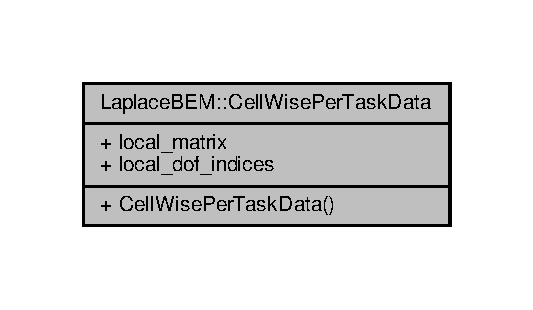
\includegraphics[width=256pt]{structLaplaceBEM_1_1CellWisePerTaskData__coll__graph}
\end{center}
\end{figure}
\subsection*{Public Member Functions}
\begin{DoxyCompactItemize}
\item 
\mbox{\Hypertarget{structLaplaceBEM_1_1CellWisePerTaskData_aa0a2b02ed445e552f28796e19172512f}\label{structLaplaceBEM_1_1CellWisePerTaskData_aa0a2b02ed445e552f28796e19172512f}} 
{\bfseries Cell\+Wise\+Per\+Task\+Data} (const Finite\+Element$<$ 2, 3 $>$ \&fe)
\end{DoxyCompactItemize}
\subsection*{Public Attributes}
\begin{DoxyCompactItemize}
\item 
\mbox{\Hypertarget{structLaplaceBEM_1_1CellWisePerTaskData_a20e59a8c53ea438aa2f9781f3fdd3c37}\label{structLaplaceBEM_1_1CellWisePerTaskData_a20e59a8c53ea438aa2f9781f3fdd3c37}} 
Full\+Matrix$<$ double $>$ {\bfseries local\+\_\+matrix}
\item 
\mbox{\Hypertarget{structLaplaceBEM_1_1CellWisePerTaskData_a1b32f3d5de8e14dabb6e758311c69a9d}\label{structLaplaceBEM_1_1CellWisePerTaskData_a1b32f3d5de8e14dabb6e758311c69a9d}} 
std\+::vector$<$ types\+::global\+\_\+dof\+\_\+index $>$ {\bfseries local\+\_\+dof\+\_\+indices}
\end{DoxyCompactItemize}


\subsection{Detailed Description}
Structure holding cell-\/wise local matrix data and DoF indices, which is used for S\+MP parallel computation of the term \$(v, \{1\}\{2\}u)\$. 

The documentation for this struct was generated from the following file\+:\begin{DoxyCompactItemize}
\item 
/home/jihuan/\+Projects/deal.\+ii/program/dealii-\/9.\+1.\+1/examples/laplace-\/bem/include/\hyperlink{laplace__bem_8h}{laplace\+\_\+bem.\+h}\end{DoxyCompactItemize}

\hypertarget{structLaplaceBEM_1_1CellWiseScratchData}{}\section{Laplace\+B\+EM\+:\+:Cell\+Wise\+Scratch\+Data Struct Reference}
\label{structLaplaceBEM_1_1CellWiseScratchData}\index{Laplace\+B\+E\+M\+::\+Cell\+Wise\+Scratch\+Data@{Laplace\+B\+E\+M\+::\+Cell\+Wise\+Scratch\+Data}}


{\ttfamily \#include $<$laplace\+\_\+bem.\+h$>$}



Collaboration diagram for Laplace\+B\+EM\+:\+:Cell\+Wise\+Scratch\+Data\+:\nopagebreak
\begin{figure}[H]
\begin{center}
\leavevmode
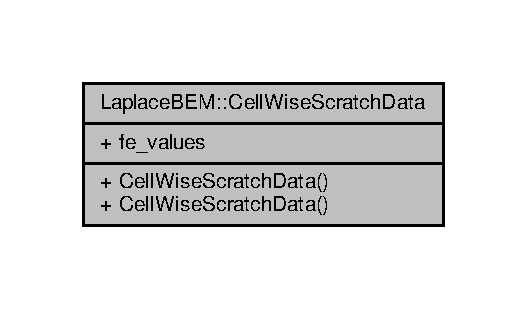
\includegraphics[width=253pt]{structLaplaceBEM_1_1CellWiseScratchData__coll__graph}
\end{center}
\end{figure}
\subsection*{Public Member Functions}
\begin{DoxyCompactItemize}
\item 
\hyperlink{structLaplaceBEM_1_1CellWiseScratchData_a8c68ff088ad75f1e448ef566aca92c68}{Cell\+Wise\+Scratch\+Data} (const Finite\+Element$<$ 2, 3 $>$ \&fe, const Quadrature$<$ 2 $>$ \&quadrature, const Update\+Flags update\+\_\+flags)
\item 
\hyperlink{structLaplaceBEM_1_1CellWiseScratchData_a79b511c5ed570ee3ec98c5891299fd7f}{Cell\+Wise\+Scratch\+Data} (const \hyperlink{structLaplaceBEM_1_1CellWiseScratchData}{Cell\+Wise\+Scratch\+Data} \&scratch\+\_\+data)
\end{DoxyCompactItemize}
\subsection*{Public Attributes}
\begin{DoxyCompactItemize}
\item 
\mbox{\Hypertarget{structLaplaceBEM_1_1CellWiseScratchData_a0ce455399dde0e15e30cbe62bf8ebb13}\label{structLaplaceBEM_1_1CellWiseScratchData_a0ce455399dde0e15e30cbe62bf8ebb13}} 
F\+E\+Values$<$ 2, 3 $>$ {\bfseries fe\+\_\+values}
\end{DoxyCompactItemize}


\subsection{Detailed Description}
Structure holding temporary data which are needed for cell-\/wise integration for the term \$(v, \{1\}\{2\}u)\$. 

\subsection{Constructor \& Destructor Documentation}
\mbox{\Hypertarget{structLaplaceBEM_1_1CellWiseScratchData_a8c68ff088ad75f1e448ef566aca92c68}\label{structLaplaceBEM_1_1CellWiseScratchData_a8c68ff088ad75f1e448ef566aca92c68}} 
\index{Laplace\+B\+E\+M\+::\+Cell\+Wise\+Scratch\+Data@{Laplace\+B\+E\+M\+::\+Cell\+Wise\+Scratch\+Data}!Cell\+Wise\+Scratch\+Data@{Cell\+Wise\+Scratch\+Data}}
\index{Cell\+Wise\+Scratch\+Data@{Cell\+Wise\+Scratch\+Data}!Laplace\+B\+E\+M\+::\+Cell\+Wise\+Scratch\+Data@{Laplace\+B\+E\+M\+::\+Cell\+Wise\+Scratch\+Data}}
\subsubsection{\texorpdfstring{Cell\+Wise\+Scratch\+Data()}{CellWiseScratchData()}\hspace{0.1cm}{\footnotesize\ttfamily [1/2]}}
{\footnotesize\ttfamily Laplace\+B\+E\+M\+::\+Cell\+Wise\+Scratch\+Data\+::\+Cell\+Wise\+Scratch\+Data (\begin{DoxyParamCaption}\item[{const Finite\+Element$<$ 2, 3 $>$ \&}]{fe,  }\item[{const Quadrature$<$ 2 $>$ \&}]{quadrature,  }\item[{const Update\+Flags}]{update\+\_\+flags }\end{DoxyParamCaption})\hspace{0.3cm}{\ttfamily [inline]}}

Constructor for the structure. 
\begin{DoxyParams}{Parameters}
{\em fe} & \\
\hline
{\em quadrature} & \\
\hline
{\em update\+\_\+flags} & \\
\hline
\end{DoxyParams}
\mbox{\Hypertarget{structLaplaceBEM_1_1CellWiseScratchData_a79b511c5ed570ee3ec98c5891299fd7f}\label{structLaplaceBEM_1_1CellWiseScratchData_a79b511c5ed570ee3ec98c5891299fd7f}} 
\index{Laplace\+B\+E\+M\+::\+Cell\+Wise\+Scratch\+Data@{Laplace\+B\+E\+M\+::\+Cell\+Wise\+Scratch\+Data}!Cell\+Wise\+Scratch\+Data@{Cell\+Wise\+Scratch\+Data}}
\index{Cell\+Wise\+Scratch\+Data@{Cell\+Wise\+Scratch\+Data}!Laplace\+B\+E\+M\+::\+Cell\+Wise\+Scratch\+Data@{Laplace\+B\+E\+M\+::\+Cell\+Wise\+Scratch\+Data}}
\subsubsection{\texorpdfstring{Cell\+Wise\+Scratch\+Data()}{CellWiseScratchData()}\hspace{0.1cm}{\footnotesize\ttfamily [2/2]}}
{\footnotesize\ttfamily Laplace\+B\+E\+M\+::\+Cell\+Wise\+Scratch\+Data\+::\+Cell\+Wise\+Scratch\+Data (\begin{DoxyParamCaption}\item[{const \hyperlink{structLaplaceBEM_1_1CellWiseScratchData}{Cell\+Wise\+Scratch\+Data} \&}]{scratch\+\_\+data }\end{DoxyParamCaption})\hspace{0.3cm}{\ttfamily [inline]}}

Copy constructor for the structure. Because {\ttfamily F\+E\+Values} is neither copyable nor has it copy constructor, this copy constructor is mandatory for replication into each task. 
\begin{DoxyParams}{Parameters}
{\em scratch\+\_\+data} & \\
\hline
\end{DoxyParams}


The documentation for this struct was generated from the following file\+:\begin{DoxyCompactItemize}
\item 
/home/jihuan/\+Projects/deal.\+ii/program/dealii-\/9.\+1.\+1/examples/laplace-\/bem/include/\hyperlink{laplace__bem_8h}{laplace\+\_\+bem.\+h}\end{DoxyCompactItemize}

\hypertarget{classCluster}{}\section{Cluster$<$ spacedim, Number $>$ Class Template Reference}
\label{classCluster}\index{Cluster$<$ spacedim, Number $>$@{Cluster$<$ spacedim, Number $>$}}


Class for an index cluster.  




{\ttfamily \#include $<$cluster.\+h$>$}



Collaboration diagram for Cluster$<$ spacedim, Number $>$\+:\nopagebreak
\begin{figure}[H]
\begin{center}
\leavevmode
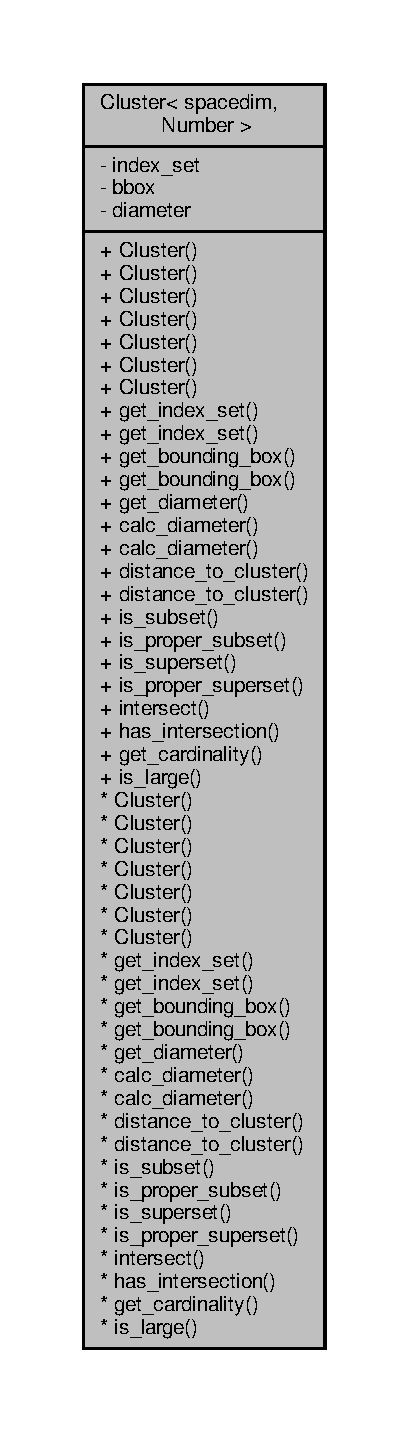
\includegraphics[height=550pt]{classCluster__coll__graph}
\end{center}
\end{figure}
\subsection*{Public Member Functions}
\textbf{ }\par
\begin{DoxyCompactItemize}
\item 
\hyperlink{classCluster_a214163f431f0bd9840d14bbebcc087e7}{Cluster} ()
\item 
\hyperlink{classCluster_aa87c73e27c410b04415e5ff1b026ae74}{Cluster} (const std\+::vector$<$ types\+::global\+\_\+dof\+\_\+index $>$ \&index\+\_\+set)
\item 
\hyperlink{classCluster_a157b06089b0f866a754a8e3a3aa49fd9}{Cluster} (const std\+::vector$<$ types\+::global\+\_\+dof\+\_\+index $>$ \&index\+\_\+set, const std\+::vector$<$ Point$<$ spacedim, Number $>$$>$ \&all\+\_\+support\+\_\+points)
\item 
\hyperlink{classCluster_a07a5837c2f6c0b676ca45b826e51b460}{Cluster} (const std\+::vector$<$ types\+::global\+\_\+dof\+\_\+index $>$ \&index\+\_\+set, const std\+::vector$<$ Point$<$ spacedim, Number $>$$>$ \&all\+\_\+support\+\_\+points, const std\+::vector$<$ Number $>$ \&cell\+\_\+size\+\_\+at\+\_\+dofs)
\item 
\hyperlink{classCluster_aaa9ac4c5b6df1633980e45c3076e17e0}{Cluster} (const std\+::vector$<$ types\+::global\+\_\+dof\+\_\+index $>$ \&index\+\_\+set, const \hyperlink{classSimpleBoundingBox}{Simple\+Bounding\+Box}$<$ spacedim, Number $>$ \&bbox, const std\+::vector$<$ Point$<$ spacedim, Number $>$$>$ \&all\+\_\+support\+\_\+points)
\item 
\hyperlink{classCluster_adf806cf8bccb891707d8e7d4c345518b}{Cluster} (const std\+::vector$<$ types\+::global\+\_\+dof\+\_\+index $>$ \&index\+\_\+set, const \hyperlink{classSimpleBoundingBox}{Simple\+Bounding\+Box}$<$ spacedim, Number $>$ \&bbox, const std\+::vector$<$ Point$<$ spacedim, Number $>$$>$ \&all\+\_\+support\+\_\+points, const std\+::vector$<$ Number $>$ \&cell\+\_\+size\+\_\+at\+\_\+dofs)
\item 
\hyperlink{classCluster_a27a372b05916f136ff9fe3e5a92a4362}{Cluster} (const \hyperlink{classCluster}{Cluster}$<$ spacedim, Number $>$ \&cluster)
\item 
std\+::vector$<$ types\+::global\+\_\+dof\+\_\+index $>$ \& \hyperlink{classCluster_ada8786f2258b9fbeed2ed04bc1007c89}{get\+\_\+index\+\_\+set} ()
\item 
const std\+::vector$<$ types\+::global\+\_\+dof\+\_\+index $>$ \& \hyperlink{classCluster_acd4c3a1c712aca32cffefb64f88a1b08}{get\+\_\+index\+\_\+set} () const
\item 
\hyperlink{classSimpleBoundingBox}{Simple\+Bounding\+Box}$<$ spacedim, Number $>$ \& \hyperlink{classCluster_a062a81f89fcb644c98f94fdf20ebcced}{get\+\_\+bounding\+\_\+box} ()
\item 
const \hyperlink{classSimpleBoundingBox}{Simple\+Bounding\+Box}$<$ spacedim, Number $>$ \& \hyperlink{classCluster_ad720b2126e07c5698c1fc39ac3f1e6a4}{get\+\_\+bounding\+\_\+box} () const
\item 
Number \hyperlink{classCluster_aab3f02640b57812eb697c39e8c4cc2e3}{get\+\_\+diameter} () const
\item 
Number \hyperlink{classCluster_a2204e6b5cf593d9e93a56f9269d74b4c}{calc\+\_\+diameter} (const std\+::vector$<$ Point$<$ spacedim, Number $>$$>$ \&all\+\_\+support\+\_\+points) const
\item 
Number \hyperlink{classCluster_ab9900a870bdd05d4638b820716e03293}{calc\+\_\+diameter} (const std\+::vector$<$ Point$<$ spacedim, Number $>$$>$ \&all\+\_\+support\+\_\+points, const std\+::vector$<$ Number $>$ \&cell\+\_\+size\+\_\+at\+\_\+dofs) const
\item 
Number \hyperlink{classCluster_aba84e3743344f360ccdb855037e1b45e}{distance\+\_\+to\+\_\+cluster} (const \hyperlink{classCluster}{Cluster} \&cluster, const std\+::vector$<$ Point$<$ spacedim, Number $>$$>$ \&all\+\_\+support\+\_\+points) const
\item 
Number \hyperlink{classCluster_a1eeffaea84b84d0288544dd4ff007d7b}{distance\+\_\+to\+\_\+cluster} (const \hyperlink{classCluster}{Cluster} \&cluster, const std\+::vector$<$ Point$<$ spacedim, Number $>$$>$ \&all\+\_\+support\+\_\+points, const std\+::vector$<$ Number $>$ \&cell\+\_\+size\+\_\+at\+\_\+dofs) const
\item 
bool \hyperlink{classCluster_a8cbdd8366b60c14f44a951ebfe024bb5}{is\+\_\+subset} (const \hyperlink{classCluster}{Cluster} \&cluster) const
\item 
bool \hyperlink{classCluster_aaf45b6f7d9e629dd2fe648dd0231a559}{is\+\_\+proper\+\_\+subset} (const \hyperlink{classCluster}{Cluster} \&cluster) const
\item 
bool \hyperlink{classCluster_abdc3b12ac53ba6fba8479a9bbd9b6aa2}{is\+\_\+superset} (const \hyperlink{classCluster}{Cluster} \&cluster) const
\item 
bool \hyperlink{classCluster_adfabc1eae12e962bae4af0a1854c3795}{is\+\_\+proper\+\_\+superset} (const \hyperlink{classCluster}{Cluster} \&cluster) const
\item 
void \hyperlink{classCluster_a47961c1b0a34b58266aa3bd87fd36b32}{intersect} (const \hyperlink{classCluster}{Cluster} \&cluster, std\+::vector$<$ types\+::global\+\_\+dof\+\_\+index $>$ \&index\+\_\+set\+\_\+intersection) const
\item 
bool \hyperlink{classCluster_ad70ce1f046bb3b47fff585eaf6ec4856}{has\+\_\+intersection} (const \hyperlink{classCluster}{Cluster} \&cluster) const
\item 
std\+::size\+\_\+t \hyperlink{classCluster_a7fd600d238aa703f40407e609c08fec6}{get\+\_\+cardinality} () const
\item 
bool \hyperlink{classCluster_a55c608dd38d185c394e516d106fea02a}{is\+\_\+large} (unsigned int n\+\_\+min) const
\end{DoxyCompactItemize}

\subsection*{Private Attributes}
\begin{DoxyCompactItemize}
\item 
\mbox{\Hypertarget{classCluster_a93791a440f03b43cdfa89e48be33cddb}\label{classCluster_a93791a440f03b43cdfa89e48be33cddb}} 
std\+::vector$<$ types\+::global\+\_\+dof\+\_\+index $>$ {\bfseries index\+\_\+set}
\item 
\mbox{\Hypertarget{classCluster_ac0332366e2e144f5a97cb19a8bbdec71}\label{classCluster_ac0332366e2e144f5a97cb19a8bbdec71}} 
\hyperlink{classSimpleBoundingBox}{Simple\+Bounding\+Box}$<$ spacedim, Number $>$ {\bfseries bbox}
\item 
\mbox{\Hypertarget{classCluster_aa3689e19cea2145941c6ba116fbb295c}\label{classCluster_aa3689e19cea2145941c6ba116fbb295c}} 
Number {\bfseries diameter}
\end{DoxyCompactItemize}
\subsection*{Friends}
\begin{DoxyCompactItemize}
\item 
\mbox{\Hypertarget{classCluster_ad6f759d8c7460a9c5366f195df4dc57f}\label{classCluster_ad6f759d8c7460a9c5366f195df4dc57f}} 
{\footnotesize template$<$int spacedim1, typename Number1 $>$ }\\std\+::ostream \& {\bfseries operator$<$$<$} (std\+::ostream \&out, const \hyperlink{classCluster}{Cluster}$<$ spacedim1, Number1 $>$ \&cluster)
\item 
\mbox{\Hypertarget{classCluster_af29091d511d3fa4e0118e39db2e36f21}\label{classCluster_af29091d511d3fa4e0118e39db2e36f21}} 
{\footnotesize template$<$int spacedim1, typename Number1 $>$ }\\Number1 {\bfseries calc\+\_\+cluster\+\_\+distance} (const \hyperlink{classCluster}{Cluster}$<$ spacedim1, Number1 $>$ \&cluster1, const \hyperlink{classCluster}{Cluster}$<$ spacedim1, Number1 $>$ \&cluster2, const std\+::vector$<$ Point$<$ spacedim1, Number1 $>$$>$ \&all\+\_\+support\+\_\+points)
\item 
\mbox{\Hypertarget{classCluster_aeb29e01c4bc5a919856849fae7c53b21}\label{classCluster_aeb29e01c4bc5a919856849fae7c53b21}} 
{\footnotesize template$<$int spacedim1, typename Number1 $>$ }\\Number1 {\bfseries calc\+\_\+cluster\+\_\+distance} (const \hyperlink{classCluster}{Cluster}$<$ spacedim1, Number1 $>$ \&cluster1, const \hyperlink{classCluster}{Cluster}$<$ spacedim1, Number1 $>$ \&cluster2, const std\+::vector$<$ Point$<$ spacedim1, Number1 $>$$>$ \&all\+\_\+support\+\_\+points, const std\+::vector$<$ Number1 $>$ \&cell\+\_\+size\+\_\+at\+\_\+dofs)
\item 
{\footnotesize template$<$int spacedim1, typename Number1 $>$ }\\bool \hyperlink{classCluster_a930aea4a53249004429d28f9631e495f}{operator==} (const \hyperlink{classCluster}{Cluster}$<$ spacedim1, Number1 $>$ \&cluster1, const \hyperlink{classCluster}{Cluster}$<$ spacedim1, Number1 $>$ \&cluster2)
\end{DoxyCompactItemize}


\subsection{Detailed Description}
\subsubsection*{template$<$int spacedim, typename Number = double$>$\newline
class Cluster$<$ spacedim, Number $>$}

Class for an index cluster. 

The {\ttfamily \hyperlink{classCluster}{Cluster}} class contains both the DoF index set {\ttfamily index\+\_\+set} and the corresponding bounding box {\ttfamily bbox}. 

\subsection{Constructor \& Destructor Documentation}
\mbox{\Hypertarget{classCluster_a214163f431f0bd9840d14bbebcc087e7}\label{classCluster_a214163f431f0bd9840d14bbebcc087e7}} 
\index{Cluster@{Cluster}!Cluster@{Cluster}}
\index{Cluster@{Cluster}!Cluster@{Cluster}}
\subsubsection{\texorpdfstring{Cluster()}{Cluster()}\hspace{0.1cm}{\footnotesize\ttfamily [1/7]}}
{\footnotesize\ttfamily template$<$int spacedim, typename Number $>$ \\
\hyperlink{classCluster}{Cluster}$<$ spacedim, Number $>$\+::\hyperlink{classCluster}{Cluster} (\begin{DoxyParamCaption}{ }\end{DoxyParamCaption})}

Default constructor. \mbox{\Hypertarget{classCluster_aa87c73e27c410b04415e5ff1b026ae74}\label{classCluster_aa87c73e27c410b04415e5ff1b026ae74}} 
\index{Cluster@{Cluster}!Cluster@{Cluster}}
\index{Cluster@{Cluster}!Cluster@{Cluster}}
\subsubsection{\texorpdfstring{Cluster()}{Cluster()}\hspace{0.1cm}{\footnotesize\ttfamily [2/7]}}
{\footnotesize\ttfamily template$<$int spacedim, typename Number $>$ \\
\hyperlink{classCluster}{Cluster}$<$ spacedim, Number $>$\+::\hyperlink{classCluster}{Cluster} (\begin{DoxyParamCaption}\item[{const std\+::vector$<$ types\+::global\+\_\+dof\+\_\+index $>$ \&}]{index\+\_\+set }\end{DoxyParamCaption})}

Constructor from an index set only without support points and associated bounding box. 
\begin{DoxyParams}{Parameters}
{\em index\+\_\+set} & \\
\hline
\end{DoxyParams}
\mbox{\Hypertarget{classCluster_a157b06089b0f866a754a8e3a3aa49fd9}\label{classCluster_a157b06089b0f866a754a8e3a3aa49fd9}} 
\index{Cluster@{Cluster}!Cluster@{Cluster}}
\index{Cluster@{Cluster}!Cluster@{Cluster}}
\subsubsection{\texorpdfstring{Cluster()}{Cluster()}\hspace{0.1cm}{\footnotesize\ttfamily [3/7]}}
{\footnotesize\ttfamily template$<$int spacedim, typename Number $>$ \\
\hyperlink{classCluster}{Cluster}$<$ spacedim, Number $>$\+::\hyperlink{classCluster}{Cluster} (\begin{DoxyParamCaption}\item[{const std\+::vector$<$ types\+::global\+\_\+dof\+\_\+index $>$ \&}]{index\+\_\+set,  }\item[{const std\+::vector$<$ Point$<$ spacedim, Number $>$$>$ \&}]{all\+\_\+support\+\_\+points }\end{DoxyParamCaption})}

Constructor from an index set without cluster diameter correction.

The bounding box will be recalculated. 
\begin{DoxyParams}{Parameters}
{\em index\+\_\+set} & \\
\hline
{\em all\+\_\+support\+\_\+points} & \\
\hline
\end{DoxyParams}
\mbox{\Hypertarget{classCluster_a07a5837c2f6c0b676ca45b826e51b460}\label{classCluster_a07a5837c2f6c0b676ca45b826e51b460}} 
\index{Cluster@{Cluster}!Cluster@{Cluster}}
\index{Cluster@{Cluster}!Cluster@{Cluster}}
\subsubsection{\texorpdfstring{Cluster()}{Cluster()}\hspace{0.1cm}{\footnotesize\ttfamily [4/7]}}
{\footnotesize\ttfamily template$<$int spacedim, typename Number $>$ \\
\hyperlink{classCluster}{Cluster}$<$ spacedim, Number $>$\+::\hyperlink{classCluster}{Cluster} (\begin{DoxyParamCaption}\item[{const std\+::vector$<$ types\+::global\+\_\+dof\+\_\+index $>$ \&}]{index\+\_\+set,  }\item[{const std\+::vector$<$ Point$<$ spacedim, Number $>$$>$ \&}]{all\+\_\+support\+\_\+points,  }\item[{const std\+::vector$<$ Number $>$ \&}]{cell\+\_\+size\+\_\+at\+\_\+dofs }\end{DoxyParamCaption})}

Constructor from an index set with cluster diameter correction.

The bounding box will be recalculated. 
\begin{DoxyParams}{Parameters}
{\em index\+\_\+set} & \\
\hline
{\em all\+\_\+support\+\_\+points} & \\
\hline
\end{DoxyParams}
\mbox{\Hypertarget{classCluster_aaa9ac4c5b6df1633980e45c3076e17e0}\label{classCluster_aaa9ac4c5b6df1633980e45c3076e17e0}} 
\index{Cluster@{Cluster}!Cluster@{Cluster}}
\index{Cluster@{Cluster}!Cluster@{Cluster}}
\subsubsection{\texorpdfstring{Cluster()}{Cluster()}\hspace{0.1cm}{\footnotesize\ttfamily [5/7]}}
{\footnotesize\ttfamily template$<$int spacedim, typename Number $>$ \\
\hyperlink{classCluster}{Cluster}$<$ spacedim, Number $>$\+::\hyperlink{classCluster}{Cluster} (\begin{DoxyParamCaption}\item[{const std\+::vector$<$ types\+::global\+\_\+dof\+\_\+index $>$ \&}]{index\+\_\+set,  }\item[{const \hyperlink{classSimpleBoundingBox}{Simple\+Bounding\+Box}$<$ spacedim, Number $>$ \&}]{bbox,  }\item[{const std\+::vector$<$ Point$<$ spacedim, Number $>$$>$ \&}]{all\+\_\+support\+\_\+points }\end{DoxyParamCaption})}

Constructor from an index set and a bounding box without cluster diameter correction.

The input bounding box will be copied into the cluster without recalculation. However, the diameter of the cluster is recalculated. 
\begin{DoxyParams}{Parameters}
{\em index\+\_\+set} & \\
\hline
{\em bbox} & \\
\hline
\end{DoxyParams}
\mbox{\Hypertarget{classCluster_adf806cf8bccb891707d8e7d4c345518b}\label{classCluster_adf806cf8bccb891707d8e7d4c345518b}} 
\index{Cluster@{Cluster}!Cluster@{Cluster}}
\index{Cluster@{Cluster}!Cluster@{Cluster}}
\subsubsection{\texorpdfstring{Cluster()}{Cluster()}\hspace{0.1cm}{\footnotesize\ttfamily [6/7]}}
{\footnotesize\ttfamily template$<$int spacedim, typename Number $>$ \\
\hyperlink{classCluster}{Cluster}$<$ spacedim, Number $>$\+::\hyperlink{classCluster}{Cluster} (\begin{DoxyParamCaption}\item[{const std\+::vector$<$ types\+::global\+\_\+dof\+\_\+index $>$ \&}]{index\+\_\+set,  }\item[{const \hyperlink{classSimpleBoundingBox}{Simple\+Bounding\+Box}$<$ spacedim, Number $>$ \&}]{bbox,  }\item[{const std\+::vector$<$ Point$<$ spacedim, Number $>$$>$ \&}]{all\+\_\+support\+\_\+points,  }\item[{const std\+::vector$<$ Number $>$ \&}]{cell\+\_\+size\+\_\+at\+\_\+dofs }\end{DoxyParamCaption})}

Constructor from an index set and a bounding box with cluster diameter correction.

The input bounding box will be copied into the cluster without recalculation. However, the diameter of the cluster is recalculated. 
\begin{DoxyParams}{Parameters}
{\em index\+\_\+set} & \\
\hline
{\em bbox} & \\
\hline
\end{DoxyParams}
\mbox{\Hypertarget{classCluster_a27a372b05916f136ff9fe3e5a92a4362}\label{classCluster_a27a372b05916f136ff9fe3e5a92a4362}} 
\index{Cluster@{Cluster}!Cluster@{Cluster}}
\index{Cluster@{Cluster}!Cluster@{Cluster}}
\subsubsection{\texorpdfstring{Cluster()}{Cluster()}\hspace{0.1cm}{\footnotesize\ttfamily [7/7]}}
{\footnotesize\ttfamily template$<$int spacedim, typename Number $>$ \\
\hyperlink{classCluster}{Cluster}$<$ spacedim, Number $>$\+::\hyperlink{classCluster}{Cluster} (\begin{DoxyParamCaption}\item[{const \hyperlink{classCluster}{Cluster}$<$ spacedim, Number $>$ \&}]{cluster }\end{DoxyParamCaption})}

Copy constructor. 

\subsection{Member Function Documentation}
\mbox{\Hypertarget{classCluster_a2204e6b5cf593d9e93a56f9269d74b4c}\label{classCluster_a2204e6b5cf593d9e93a56f9269d74b4c}} 
\index{Cluster@{Cluster}!calc\+\_\+diameter@{calc\+\_\+diameter}}
\index{calc\+\_\+diameter@{calc\+\_\+diameter}!Cluster@{Cluster}}
\subsubsection{\texorpdfstring{calc\+\_\+diameter()}{calc\_diameter()}\hspace{0.1cm}{\footnotesize\ttfamily [1/2]}}
{\footnotesize\ttfamily template$<$int spacedim, typename Number $>$ \\
Number \hyperlink{classCluster}{Cluster}$<$ spacedim, Number $>$\+::calc\+\_\+diameter (\begin{DoxyParamCaption}\item[{const std\+::vector$<$ Point$<$ spacedim, Number $>$$>$ \&}]{all\+\_\+support\+\_\+points }\end{DoxyParamCaption}) const}

Calculate the diameter of the cluster. There is no cell size correction. Calculate the number of point pairs in the cluster. Let $[0, 1, 2, 3, 4, 5]$ be the indices of support points in the cluster, whose pairwise inter-\/distance will be calculated. The calculation is only needed for the marked pairs of points as shown below.


\begin{DoxyCode}
  0 1 2 3 4 5
0   - - - - -
1     - - - -
2       - - -
3         - -
4           -
5
\end{DoxyCode}


Therefore, the total number of effective point pairs is $\frac{n^2 - n}{2}$.

Referenced by Cluster$<$ spacedim, Number $>$\+::calc\+\_\+diameter().

\mbox{\Hypertarget{classCluster_ab9900a870bdd05d4638b820716e03293}\label{classCluster_ab9900a870bdd05d4638b820716e03293}} 
\index{Cluster@{Cluster}!calc\+\_\+diameter@{calc\+\_\+diameter}}
\index{calc\+\_\+diameter@{calc\+\_\+diameter}!Cluster@{Cluster}}
\subsubsection{\texorpdfstring{calc\+\_\+diameter()}{calc\_diameter()}\hspace{0.1cm}{\footnotesize\ttfamily [2/2]}}
{\footnotesize\ttfamily template$<$int spacedim, typename Number $>$ \\
Number \hyperlink{classCluster}{Cluster}$<$ spacedim, Number $>$\+::calc\+\_\+diameter (\begin{DoxyParamCaption}\item[{const std\+::vector$<$ Point$<$ spacedim, Number $>$$>$ \&}]{all\+\_\+support\+\_\+points,  }\item[{const std\+::vector$<$ Number $>$ \&}]{cell\+\_\+size\+\_\+at\+\_\+dofs }\end{DoxyParamCaption}) const}

Calculate the diameter of the cluster. Cell size correction is applied.

N.\+B. Doubled estimated cell size is adopted as an approximation of the support set diameter ${\rm diam}(Q_j)$. The correction is calculated according to the following formula. \[ \widetilde{\rm diam}(\tau) := {\rm diam}(\hat{Q}_{\tau}) + \max_{j \in \tau} {\rm diam}(Q_j) \] 
\begin{DoxyParams}{Parameters}
{\em all\+\_\+support\+\_\+points} & \\
\hline
{\em cell\+\_\+size\+\_\+at\+\_\+dofs} & \\
\hline
\end{DoxyParams}
\begin{DoxyReturn}{Returns}

\end{DoxyReturn}


References Cluster$<$ spacedim, Number $>$\+::calc\+\_\+diameter().

\mbox{\Hypertarget{classCluster_aba84e3743344f360ccdb855037e1b45e}\label{classCluster_aba84e3743344f360ccdb855037e1b45e}} 
\index{Cluster@{Cluster}!distance\+\_\+to\+\_\+cluster@{distance\+\_\+to\+\_\+cluster}}
\index{distance\+\_\+to\+\_\+cluster@{distance\+\_\+to\+\_\+cluster}!Cluster@{Cluster}}
\subsubsection{\texorpdfstring{distance\+\_\+to\+\_\+cluster()}{distance\_to\_cluster()}\hspace{0.1cm}{\footnotesize\ttfamily [1/2]}}
{\footnotesize\ttfamily template$<$int spacedim, typename Number $>$ \\
Number \hyperlink{classCluster}{Cluster}$<$ spacedim, Number $>$\+::distance\+\_\+to\+\_\+cluster (\begin{DoxyParamCaption}\item[{const \hyperlink{classCluster}{Cluster}$<$ spacedim, Number $>$ \&}]{cluster,  }\item[{const std\+::vector$<$ Point$<$ spacedim, Number $>$$>$ \&}]{all\+\_\+support\+\_\+points }\end{DoxyParamCaption}) const}

Calculate the minimum distance of the current cluster to the given cluster. There is no cell size correction. \mbox{\Hypertarget{classCluster_a1eeffaea84b84d0288544dd4ff007d7b}\label{classCluster_a1eeffaea84b84d0288544dd4ff007d7b}} 
\index{Cluster@{Cluster}!distance\+\_\+to\+\_\+cluster@{distance\+\_\+to\+\_\+cluster}}
\index{distance\+\_\+to\+\_\+cluster@{distance\+\_\+to\+\_\+cluster}!Cluster@{Cluster}}
\subsubsection{\texorpdfstring{distance\+\_\+to\+\_\+cluster()}{distance\_to\_cluster()}\hspace{0.1cm}{\footnotesize\ttfamily [2/2]}}
{\footnotesize\ttfamily template$<$int spacedim, typename Number $>$ \\
Number \hyperlink{classCluster}{Cluster}$<$ spacedim, Number $>$\+::distance\+\_\+to\+\_\+cluster (\begin{DoxyParamCaption}\item[{const \hyperlink{classCluster}{Cluster}$<$ spacedim, Number $>$ \&}]{cluster,  }\item[{const std\+::vector$<$ Point$<$ spacedim, Number $>$$>$ \&}]{all\+\_\+support\+\_\+points,  }\item[{const std\+::vector$<$ Number $>$ \&}]{cell\+\_\+size\+\_\+at\+\_\+dofs }\end{DoxyParamCaption}) const}

Calculate the minimum distance of the current cluster to the given cluster. Cell size correction is applied. \mbox{\Hypertarget{classCluster_a062a81f89fcb644c98f94fdf20ebcced}\label{classCluster_a062a81f89fcb644c98f94fdf20ebcced}} 
\index{Cluster@{Cluster}!get\+\_\+bounding\+\_\+box@{get\+\_\+bounding\+\_\+box}}
\index{get\+\_\+bounding\+\_\+box@{get\+\_\+bounding\+\_\+box}!Cluster@{Cluster}}
\subsubsection{\texorpdfstring{get\+\_\+bounding\+\_\+box()}{get\_bounding\_box()}\hspace{0.1cm}{\footnotesize\ttfamily [1/2]}}
{\footnotesize\ttfamily template$<$int spacedim, typename Number $>$ \\
\hyperlink{classSimpleBoundingBox}{Simple\+Bounding\+Box}$<$ spacedim, Number $>$ \& \hyperlink{classCluster}{Cluster}$<$ spacedim, Number $>$\+::get\+\_\+bounding\+\_\+box (\begin{DoxyParamCaption}{ }\end{DoxyParamCaption})}

Get the reference to the bounding box. \mbox{\Hypertarget{classCluster_ad720b2126e07c5698c1fc39ac3f1e6a4}\label{classCluster_ad720b2126e07c5698c1fc39ac3f1e6a4}} 
\index{Cluster@{Cluster}!get\+\_\+bounding\+\_\+box@{get\+\_\+bounding\+\_\+box}}
\index{get\+\_\+bounding\+\_\+box@{get\+\_\+bounding\+\_\+box}!Cluster@{Cluster}}
\subsubsection{\texorpdfstring{get\+\_\+bounding\+\_\+box()}{get\_bounding\_box()}\hspace{0.1cm}{\footnotesize\ttfamily [2/2]}}
{\footnotesize\ttfamily template$<$int spacedim, typename Number $>$ \\
const \hyperlink{classSimpleBoundingBox}{Simple\+Bounding\+Box}$<$ spacedim, Number $>$ \& \hyperlink{classCluster}{Cluster}$<$ spacedim, Number $>$\+::get\+\_\+bounding\+\_\+box (\begin{DoxyParamCaption}{ }\end{DoxyParamCaption}) const}

Get the reference to the bounding box (const version). \mbox{\Hypertarget{classCluster_a7fd600d238aa703f40407e609c08fec6}\label{classCluster_a7fd600d238aa703f40407e609c08fec6}} 
\index{Cluster@{Cluster}!get\+\_\+cardinality@{get\+\_\+cardinality}}
\index{get\+\_\+cardinality@{get\+\_\+cardinality}!Cluster@{Cluster}}
\subsubsection{\texorpdfstring{get\+\_\+cardinality()}{get\_cardinality()}}
{\footnotesize\ttfamily template$<$int spacedim, typename Number $>$ \\
std\+::size\+\_\+t \hyperlink{classCluster}{Cluster}$<$ spacedim, Number $>$\+::get\+\_\+cardinality (\begin{DoxyParamCaption}{ }\end{DoxyParamCaption}) const}

Get the cardinality of the index set. \begin{DoxyReturn}{Returns}

\end{DoxyReturn}
\mbox{\Hypertarget{classCluster_aab3f02640b57812eb697c39e8c4cc2e3}\label{classCluster_aab3f02640b57812eb697c39e8c4cc2e3}} 
\index{Cluster@{Cluster}!get\+\_\+diameter@{get\+\_\+diameter}}
\index{get\+\_\+diameter@{get\+\_\+diameter}!Cluster@{Cluster}}
\subsubsection{\texorpdfstring{get\+\_\+diameter()}{get\_diameter()}}
{\footnotesize\ttfamily template$<$int spacedim, typename Number $>$ \\
Number \hyperlink{classCluster}{Cluster}$<$ spacedim, Number $>$\+::get\+\_\+diameter (\begin{DoxyParamCaption}{ }\end{DoxyParamCaption}) const}

Get the diameter of the cluster. \mbox{\Hypertarget{classCluster_ada8786f2258b9fbeed2ed04bc1007c89}\label{classCluster_ada8786f2258b9fbeed2ed04bc1007c89}} 
\index{Cluster@{Cluster}!get\+\_\+index\+\_\+set@{get\+\_\+index\+\_\+set}}
\index{get\+\_\+index\+\_\+set@{get\+\_\+index\+\_\+set}!Cluster@{Cluster}}
\subsubsection{\texorpdfstring{get\+\_\+index\+\_\+set()}{get\_index\_set()}\hspace{0.1cm}{\footnotesize\ttfamily [1/2]}}
{\footnotesize\ttfamily template$<$int spacedim, typename Number $>$ \\
std\+::vector$<$ types\+::global\+\_\+dof\+\_\+index $>$ \& \hyperlink{classCluster}{Cluster}$<$ spacedim, Number $>$\+::get\+\_\+index\+\_\+set (\begin{DoxyParamCaption}{ }\end{DoxyParamCaption})}

Get the reference to the index set. 

Referenced by calc\+\_\+cluster\+\_\+distance().

\mbox{\Hypertarget{classCluster_acd4c3a1c712aca32cffefb64f88a1b08}\label{classCluster_acd4c3a1c712aca32cffefb64f88a1b08}} 
\index{Cluster@{Cluster}!get\+\_\+index\+\_\+set@{get\+\_\+index\+\_\+set}}
\index{get\+\_\+index\+\_\+set@{get\+\_\+index\+\_\+set}!Cluster@{Cluster}}
\subsubsection{\texorpdfstring{get\+\_\+index\+\_\+set()}{get\_index\_set()}\hspace{0.1cm}{\footnotesize\ttfamily [2/2]}}
{\footnotesize\ttfamily template$<$int spacedim, typename Number $>$ \\
const std\+::vector$<$ types\+::global\+\_\+dof\+\_\+index $>$ \& \hyperlink{classCluster}{Cluster}$<$ spacedim, Number $>$\+::get\+\_\+index\+\_\+set (\begin{DoxyParamCaption}{ }\end{DoxyParamCaption}) const}

Get the reference to the index set (const version). \mbox{\Hypertarget{classCluster_ad70ce1f046bb3b47fff585eaf6ec4856}\label{classCluster_ad70ce1f046bb3b47fff585eaf6ec4856}} 
\index{Cluster@{Cluster}!has\+\_\+intersection@{has\+\_\+intersection}}
\index{has\+\_\+intersection@{has\+\_\+intersection}!Cluster@{Cluster}}
\subsubsection{\texorpdfstring{has\+\_\+intersection()}{has\_intersection()}}
{\footnotesize\ttfamily template$<$int spacedim, typename Number $>$ \\
bool \hyperlink{classCluster}{Cluster}$<$ spacedim, Number $>$\+::has\+\_\+intersection (\begin{DoxyParamCaption}\item[{const \hyperlink{classCluster}{Cluster}$<$ spacedim, Number $>$ \&}]{cluster }\end{DoxyParamCaption}) const}

Determine if the index set of the current cluster has a nonempty intersection with the index set of the given cluster.


\begin{DoxyDescription}
\item[Note ]The index sets associated with clusters should be sorted before calling this function. In the current implementation of cluster tree construction, all the index sets have already been sorted. 
\end{DoxyDescription}
\begin{DoxyParams}{Parameters}
{\em cluster} & \\
\hline
\end{DoxyParams}
\begin{DoxyReturn}{Returns}

\end{DoxyReturn}


References Cluster$<$ spacedim, Number $>$\+::intersect().

\mbox{\Hypertarget{classCluster_a47961c1b0a34b58266aa3bd87fd36b32}\label{classCluster_a47961c1b0a34b58266aa3bd87fd36b32}} 
\index{Cluster@{Cluster}!intersect@{intersect}}
\index{intersect@{intersect}!Cluster@{Cluster}}
\subsubsection{\texorpdfstring{intersect()}{intersect()}}
{\footnotesize\ttfamily template$<$int spacedim, typename Number $>$ \\
void \hyperlink{classCluster}{Cluster}$<$ spacedim, Number $>$\+::intersect (\begin{DoxyParamCaption}\item[{const \hyperlink{classCluster}{Cluster}$<$ spacedim, Number $>$ \&}]{cluster,  }\item[{std\+::vector$<$ types\+::global\+\_\+dof\+\_\+index $>$ \&}]{index\+\_\+set\+\_\+intersection }\end{DoxyParamCaption}) const}

Calculate the intersection of the index sets of the current and the given clusters.


\begin{DoxyDescription}
\item[Note ]The index sets associated with clusters should be sorted before calling this function. In the current implementation of cluster tree construction, all the index sets have already been sorted. 
\end{DoxyDescription}
\begin{DoxyParams}{Parameters}
{\em cluster} & \\
\hline
{\em index\+\_\+set\+\_\+intersection} & \\
\hline
\end{DoxyParams}


Referenced by Cluster$<$ spacedim, Number $>$\+::has\+\_\+intersection().

\mbox{\Hypertarget{classCluster_a55c608dd38d185c394e516d106fea02a}\label{classCluster_a55c608dd38d185c394e516d106fea02a}} 
\index{Cluster@{Cluster}!is\+\_\+large@{is\+\_\+large}}
\index{is\+\_\+large@{is\+\_\+large}!Cluster@{Cluster}}
\subsubsection{\texorpdfstring{is\+\_\+large()}{is\_large()}}
{\footnotesize\ttfamily template$<$int spacedim, typename Number $>$ \\
bool \hyperlink{classCluster}{Cluster}$<$ spacedim, Number $>$\+::is\+\_\+large (\begin{DoxyParamCaption}\item[{unsigned int}]{n\+\_\+min }\end{DoxyParamCaption}) const}

Determine if the cluster is large enough.


\begin{DoxyParams}{Parameters}
{\em n\+\_\+min} & The size threshold value for determining if a cluster is large. \\
\hline
\end{DoxyParams}
\begin{DoxyReturn}{Returns}

\end{DoxyReturn}


References Cluster$<$ spacedim, Number $>$\+::operator==.

\mbox{\Hypertarget{classCluster_aaf45b6f7d9e629dd2fe648dd0231a559}\label{classCluster_aaf45b6f7d9e629dd2fe648dd0231a559}} 
\index{Cluster@{Cluster}!is\+\_\+proper\+\_\+subset@{is\+\_\+proper\+\_\+subset}}
\index{is\+\_\+proper\+\_\+subset@{is\+\_\+proper\+\_\+subset}!Cluster@{Cluster}}
\subsubsection{\texorpdfstring{is\+\_\+proper\+\_\+subset()}{is\_proper\_subset()}}
{\footnotesize\ttfamily template$<$int spacedim, typename Number $>$ \\
bool \hyperlink{classCluster}{Cluster}$<$ spacedim, Number $>$\+::is\+\_\+proper\+\_\+subset (\begin{DoxyParamCaption}\item[{const \hyperlink{classCluster}{Cluster}$<$ spacedim, Number $>$ \&}]{cluster }\end{DoxyParamCaption}) const}

Check if the index set of the current cluster is a proper subset of that of the given cluster.


\begin{DoxyDescription}
\item[Note ]The index sets associated with clusters should be sorted before calling this function. In the current implementation of cluster tree construction, all the index sets have already been sorted. 
\end{DoxyDescription}
\begin{DoxyParams}{Parameters}
{\em cluster} & \\
\hline
\end{DoxyParams}
\begin{DoxyReturn}{Returns}

\end{DoxyReturn}
\mbox{\Hypertarget{classCluster_adfabc1eae12e962bae4af0a1854c3795}\label{classCluster_adfabc1eae12e962bae4af0a1854c3795}} 
\index{Cluster@{Cluster}!is\+\_\+proper\+\_\+superset@{is\+\_\+proper\+\_\+superset}}
\index{is\+\_\+proper\+\_\+superset@{is\+\_\+proper\+\_\+superset}!Cluster@{Cluster}}
\subsubsection{\texorpdfstring{is\+\_\+proper\+\_\+superset()}{is\_proper\_superset()}}
{\footnotesize\ttfamily template$<$int spacedim, typename Number $>$ \\
bool \hyperlink{classCluster}{Cluster}$<$ spacedim, Number $>$\+::is\+\_\+proper\+\_\+superset (\begin{DoxyParamCaption}\item[{const \hyperlink{classCluster}{Cluster}$<$ spacedim, Number $>$ \&}]{cluster }\end{DoxyParamCaption}) const}

Check if the index set of the current cluster is a proper superset of that of the given cluster.


\begin{DoxyDescription}
\item[Note ]The index sets associated with clusters should be sorted before calling this function. In the current implementation of cluster tree construction, all the index sets have already been sorted. 
\end{DoxyDescription}
\begin{DoxyParams}{Parameters}
{\em cluster} & \\
\hline
\end{DoxyParams}
\begin{DoxyReturn}{Returns}

\end{DoxyReturn}
\mbox{\Hypertarget{classCluster_a8cbdd8366b60c14f44a951ebfe024bb5}\label{classCluster_a8cbdd8366b60c14f44a951ebfe024bb5}} 
\index{Cluster@{Cluster}!is\+\_\+subset@{is\+\_\+subset}}
\index{is\+\_\+subset@{is\+\_\+subset}!Cluster@{Cluster}}
\subsubsection{\texorpdfstring{is\+\_\+subset()}{is\_subset()}}
{\footnotesize\ttfamily template$<$int spacedim, typename Number $>$ \\
bool \hyperlink{classCluster}{Cluster}$<$ spacedim, Number $>$\+::is\+\_\+subset (\begin{DoxyParamCaption}\item[{const \hyperlink{classCluster}{Cluster}$<$ spacedim, Number $>$ \&}]{cluster }\end{DoxyParamCaption}) const}

Check if the index set of the current cluster is a subset of that of the given cluster.


\begin{DoxyDescription}
\item[Note ]The index sets associated with clusters should be sorted before calling this function. In the current implementation of cluster tree construction, all the index sets have already been sorted. 
\end{DoxyDescription}
\begin{DoxyParams}{Parameters}
{\em cluster} & \\
\hline
\end{DoxyParams}
\begin{DoxyReturn}{Returns}

\end{DoxyReturn}
\mbox{\Hypertarget{classCluster_abdc3b12ac53ba6fba8479a9bbd9b6aa2}\label{classCluster_abdc3b12ac53ba6fba8479a9bbd9b6aa2}} 
\index{Cluster@{Cluster}!is\+\_\+superset@{is\+\_\+superset}}
\index{is\+\_\+superset@{is\+\_\+superset}!Cluster@{Cluster}}
\subsubsection{\texorpdfstring{is\+\_\+superset()}{is\_superset()}}
{\footnotesize\ttfamily template$<$int spacedim, typename Number $>$ \\
bool \hyperlink{classCluster}{Cluster}$<$ spacedim, Number $>$\+::is\+\_\+superset (\begin{DoxyParamCaption}\item[{const \hyperlink{classCluster}{Cluster}$<$ spacedim, Number $>$ \&}]{cluster }\end{DoxyParamCaption}) const}

Check if the index set of the current cluster is a superset of that of the given cluster.


\begin{DoxyDescription}
\item[Note ]The index sets associated with clusters should be sorted before calling this function. In the current implementation of cluster tree construction, all the index sets have already been sorted. 
\end{DoxyDescription}
\begin{DoxyParams}{Parameters}
{\em cluster} & \\
\hline
\end{DoxyParams}
\begin{DoxyReturn}{Returns}

\end{DoxyReturn}


\subsection{Friends And Related Function Documentation}
\mbox{\Hypertarget{classCluster_a930aea4a53249004429d28f9631e495f}\label{classCluster_a930aea4a53249004429d28f9631e495f}} 
\index{Cluster@{Cluster}!operator==@{operator==}}
\index{operator==@{operator==}!Cluster@{Cluster}}
\subsubsection{\texorpdfstring{operator==}{operator==}}
{\footnotesize\ttfamily template$<$int spacedim, typename Number = double$>$ \\
template$<$int spacedim1, typename Number1 $>$ \\
bool operator== (\begin{DoxyParamCaption}\item[{const \hyperlink{classCluster}{Cluster}$<$ spacedim1, Number1 $>$ \&}]{cluster1,  }\item[{const \hyperlink{classCluster}{Cluster}$<$ spacedim1, Number1 $>$ \&}]{cluster2 }\end{DoxyParamCaption})\hspace{0.3cm}{\ttfamily [friend]}}

Check the equality of two clusters by comparing their index sets.

This function firstly check the equality of the sizes/cardinalities of the index sets in the two clusters. If their sizes are equal, then check the contents.


\begin{DoxyParams}{Parameters}
{\em cluster1} & \\
\hline
{\em cluster2} & \\
\hline
\end{DoxyParams}
\begin{DoxyReturn}{Returns}

\end{DoxyReturn}


Referenced by Cluster$<$ spacedim, Number $>$\+::is\+\_\+large().



The documentation for this class was generated from the following file\+:\begin{DoxyCompactItemize}
\item 
/home/jihuan/\+Projects/deal.\+ii/program/dealii-\/9.\+1.\+1/examples/laplace-\/bem/include/\hyperlink{cluster_8h}{cluster.\+h}\end{DoxyCompactItemize}

\hypertarget{classClusterTree}{}\section{Cluster\+Tree$<$ spacedim, Number $>$ Class Template Reference}
\label{classClusterTree}\index{Cluster\+Tree$<$ spacedim, Number $>$@{Cluster\+Tree$<$ spacedim, Number $>$}}


Class for cluster tree.  




{\ttfamily \#include $<$cluster\+\_\+tree.\+h$>$}



Inheritance diagram for Cluster\+Tree$<$ spacedim, Number $>$\+:\nopagebreak
\begin{figure}[H]
\begin{center}
\leavevmode
\includegraphics[height=550pt]{classClusterTree__inherit__graph}
\end{center}
\end{figure}


Collaboration diagram for Cluster\+Tree$<$ spacedim, Number $>$\+:\nopagebreak
\begin{figure}[H]
\begin{center}
\leavevmode
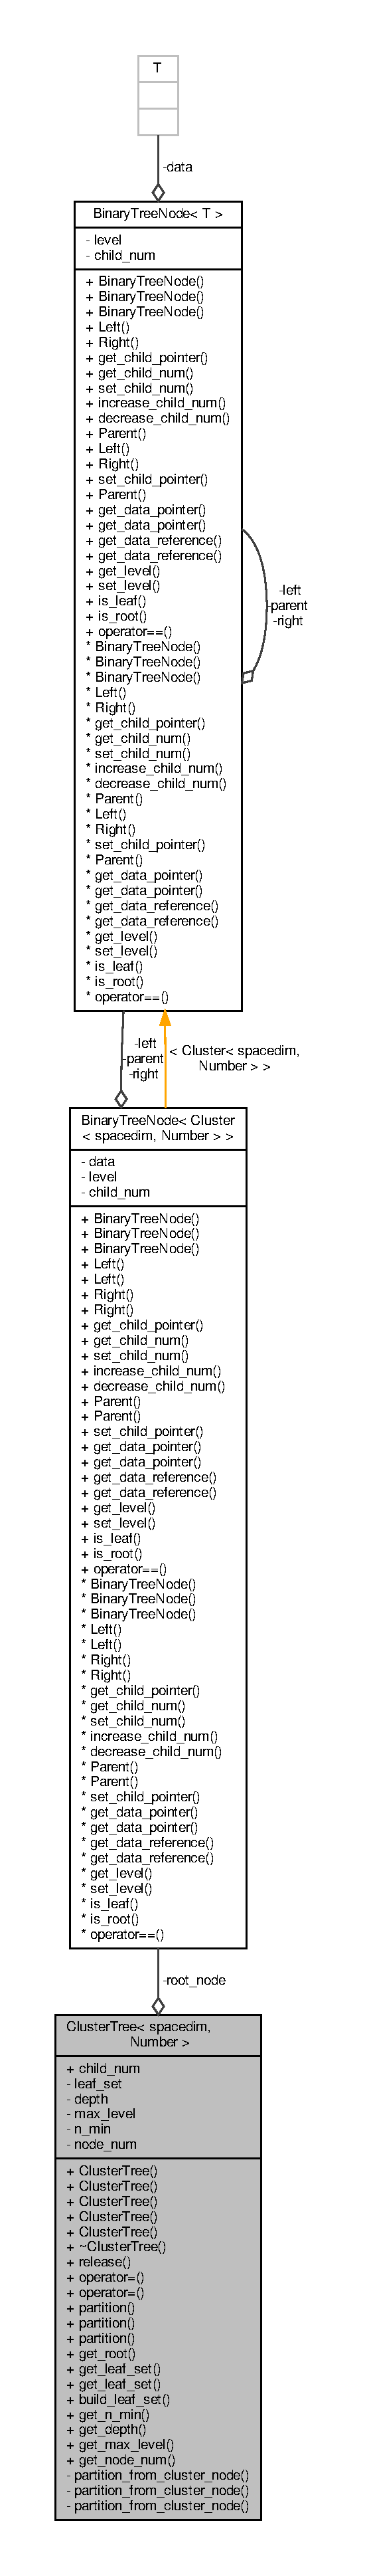
\includegraphics[height=550pt]{classClusterTree__coll__graph}
\end{center}
\end{figure}
\subsection*{Public Types}
\begin{DoxyCompactItemize}
\item 
typedef \hyperlink{classBinaryTreeNode}{Binary\+Tree\+Node}$<$ \hyperlink{classCluster}{Cluster}$<$ spacedim, Number $>$ $>$ \hyperlink{classClusterTree_ab12442ec2508818e1663df6c5a137b05}{node\+\_\+value\+\_\+type}
\item 
typedef \hyperlink{classBinaryTreeNode}{Binary\+Tree\+Node}$<$ \hyperlink{classCluster}{Cluster}$<$ spacedim, Number $>$ $>$ $\ast$ \hyperlink{classClusterTree_ae4bb0fdc7ac559d7844d04a00ab3e9de}{node\+\_\+pointer\+\_\+type}
\item 
typedef const \hyperlink{classBinaryTreeNode}{Binary\+Tree\+Node}$<$ \hyperlink{classCluster}{Cluster}$<$ spacedim, Number $>$ $>$ $\ast$ \hyperlink{classClusterTree_acb805fbc20c01a71fa6a00adc959542c}{node\+\_\+const\+\_\+pointer\+\_\+type}
\item 
typedef \hyperlink{classBinaryTreeNode}{Binary\+Tree\+Node}$<$ \hyperlink{classCluster}{Cluster}$<$ spacedim, Number $>$ $>$ \& \hyperlink{classClusterTree_a257ebe4c6eab6581a0b65ba62487ae2c}{node\+\_\+reference\+\_\+type}
\item 
typedef const \hyperlink{classBinaryTreeNode}{Binary\+Tree\+Node}$<$ \hyperlink{classCluster}{Cluster}$<$ spacedim, Number $>$ $>$ \& \hyperlink{classClusterTree_ac40955dbfdb9b0beec67a0ecf6810c8f}{node\+\_\+const\+\_\+reference\+\_\+type}
\item 
typedef \hyperlink{classCluster}{Cluster}$<$ spacedim, Number $>$ \hyperlink{classClusterTree_ab7875a0c5ba927d1d3c5f5212d1d524d}{data\+\_\+value\+\_\+type}
\item 
typedef \hyperlink{classCluster}{Cluster}$<$ spacedim, Number $>$ $\ast$ \hyperlink{classClusterTree_a87fee1708c95c5575fce3029b79d32a8}{data\+\_\+pointer\+\_\+type}
\item 
typedef const \hyperlink{classCluster}{Cluster}$<$ spacedim, Number $>$ $\ast$ \hyperlink{classClusterTree_ac425245d60967a91905245003e5d46b1}{data\+\_\+const\+\_\+pointer\+\_\+type}
\item 
typedef \hyperlink{classCluster}{Cluster}$<$ spacedim, Number $>$ \& \hyperlink{classClusterTree_ae47bb5a21c1468972b1c2ede0e8aa28c}{data\+\_\+reference\+\_\+type}
\item 
typedef const \hyperlink{classCluster}{Cluster}$<$ spacedim, Number $>$ \& \hyperlink{classClusterTree_a1d171cbb6b0a8367b4be0d2b87bc9ba8}{data\+\_\+const\+\_\+reference\+\_\+type}
\end{DoxyCompactItemize}
\subsection*{Public Member Functions}
\begin{DoxyCompactItemize}
\item 
\hyperlink{classClusterTree_a28b31e2fbe58c74eff89a1a8e2124e10}{Cluster\+Tree} ()
\item 
\hyperlink{classClusterTree_ae21fda96c7d405825a853f8759c0cc4c}{Cluster\+Tree} (const std\+::vector$<$ types\+::global\+\_\+dof\+\_\+index $>$ \&index\+\_\+set, const unsigned int \hyperlink{classClusterTree_a5af4448800c4ddc98121706754bfe3f9}{n\+\_\+min})
\item 
\hyperlink{classClusterTree_a587c465f14f7fa0e0e6a82aa8733452f}{Cluster\+Tree} (const std\+::vector$<$ types\+::global\+\_\+dof\+\_\+index $>$ \&index\+\_\+set, const std\+::vector$<$ Point$<$ spacedim $>$$>$ \&all\+\_\+support\+\_\+points, const unsigned int \hyperlink{classClusterTree_a5af4448800c4ddc98121706754bfe3f9}{n\+\_\+min})
\item 
\hyperlink{classClusterTree_a3fd518db632c62cfafb61e9ef56097c7}{Cluster\+Tree} (const std\+::vector$<$ types\+::global\+\_\+dof\+\_\+index $>$ \&index\+\_\+set, const std\+::vector$<$ Point$<$ spacedim $>$$>$ \&all\+\_\+support\+\_\+points, const std\+::vector$<$ Number $>$ \&cell\+\_\+size\+\_\+at\+\_\+dofs, const unsigned int \hyperlink{classClusterTree_a5af4448800c4ddc98121706754bfe3f9}{n\+\_\+min})
\item 
\hyperlink{classClusterTree_a40d41a3a87bee15fe2d0b39a42f705d2}{Cluster\+Tree} (const \hyperlink{classClusterTree}{Cluster\+Tree}$<$ spacedim, Number $>$ \&cluster\+\_\+tree)
\item 
\hyperlink{classClusterTree_ad1b0ac0f6474de90d4fb528b6ed28db6}{$\sim$\+Cluster\+Tree} ()
\item 
void \hyperlink{classClusterTree_a2dc8b94ebdc4e5efb885940204f614e1}{release} ()
\item 
\hyperlink{classClusterTree}{Cluster\+Tree}$<$ spacedim, Number $>$ \& \hyperlink{classClusterTree_a3a4e51a1a09f759f085ab140db914af9}{operator=} (const \hyperlink{classClusterTree}{Cluster\+Tree}$<$ spacedim, Number $>$ \&cluster\+\_\+tree)
\item 
\hyperlink{classClusterTree}{Cluster\+Tree}$<$ spacedim, Number $>$ \& \hyperlink{classClusterTree_a9700796d8fb849b3171c0c7d461a2380}{operator=} (\hyperlink{classClusterTree}{Cluster\+Tree}$<$ spacedim, Number $>$ \&\&cluster\+\_\+tree)
\item 
void \hyperlink{classClusterTree_aa514c3b75864d5f7be72315a30079cfe}{partition} ()
\item 
void \hyperlink{classClusterTree_a5657415b4b0519f045f3139d1d63e85d}{partition} (const std\+::vector$<$ Point$<$ spacedim $>$$>$ \&all\+\_\+support\+\_\+points)
\item 
void \hyperlink{classClusterTree_a4d2682986352bb1e44bc73ebfc5a9fdf}{partition} (const std\+::vector$<$ Point$<$ spacedim $>$$>$ \&all\+\_\+support\+\_\+points, const std\+::vector$<$ Number $>$ \&cell\+\_\+size\+\_\+at\+\_\+dofs)
\item 
\hyperlink{classClusterTree_ae4bb0fdc7ac559d7844d04a00ab3e9de}{node\+\_\+pointer\+\_\+type} \hyperlink{classClusterTree_a13132bfc3ca8b70af8c80066565b0adb}{get\+\_\+root} () const
\item 
std\+::vector$<$ \hyperlink{classClusterTree_ae4bb0fdc7ac559d7844d04a00ab3e9de}{node\+\_\+pointer\+\_\+type} $>$ \& \hyperlink{classClusterTree_af17a96da7f2e5391d3e49028b2aba894}{get\+\_\+leaf\+\_\+set} ()
\item 
const std\+::vector$<$ \hyperlink{classClusterTree_ae4bb0fdc7ac559d7844d04a00ab3e9de}{node\+\_\+pointer\+\_\+type} $>$ \& \hyperlink{classClusterTree_afbf8f03d5f34305d3c34ae4c360f50ae}{get\+\_\+leaf\+\_\+set} () const
\item 
void \hyperlink{classClusterTree_a1e7dc037d01b3e15f1d6b4eacac59cb1}{build\+\_\+leaf\+\_\+set} ()
\item 
unsigned int \hyperlink{classClusterTree_a403e59575a89a3e86e8d7092a8815aa5}{get\+\_\+n\+\_\+min} () const
\item 
unsigned int \hyperlink{classClusterTree_a2bd8dd175c4459338d76a8cb879afccf}{get\+\_\+depth} () const
\item 
unsigned int \hyperlink{classClusterTree_a3c1125039b1915ebad94247d6888df31}{get\+\_\+max\+\_\+level} () const
\item 
unsigned int \hyperlink{classClusterTree_af80051449b7324121fb0a27d5ce7c9a1}{get\+\_\+node\+\_\+num} () const
\end{DoxyCompactItemize}
\subsection*{Static Public Attributes}
\begin{DoxyCompactItemize}
\item 
static const unsigned int \hyperlink{classClusterTree_aa9705d3fecd5b405b804331ea031570c}{child\+\_\+num} = 2
\end{DoxyCompactItemize}
\subsection*{Private Member Functions}
\begin{DoxyCompactItemize}
\item 
void \hyperlink{classClusterTree_a8b650f0c7cc83adbde5aad9556a57ac3}{partition\+\_\+from\+\_\+cluster\+\_\+node} (\hyperlink{classClusterTree_ae4bb0fdc7ac559d7844d04a00ab3e9de}{node\+\_\+pointer\+\_\+type} current\+\_\+cluster\+\_\+node, std\+::vector$<$ \hyperlink{classClusterTree_ae4bb0fdc7ac559d7844d04a00ab3e9de}{node\+\_\+pointer\+\_\+type} $>$ \&leaf\+\_\+set\+\_\+wrt\+\_\+current\+\_\+node)
\item 
void \hyperlink{classClusterTree_a6d3636b1686d72909611a6d516f5ee47}{partition\+\_\+from\+\_\+cluster\+\_\+node} (\hyperlink{classClusterTree_ae4bb0fdc7ac559d7844d04a00ab3e9de}{node\+\_\+pointer\+\_\+type} current\+\_\+cluster\+\_\+node, const std\+::vector$<$ Point$<$ spacedim $>$$>$ \&all\+\_\+support\+\_\+points, std\+::vector$<$ \hyperlink{classClusterTree_ae4bb0fdc7ac559d7844d04a00ab3e9de}{node\+\_\+pointer\+\_\+type} $>$ \&leaf\+\_\+set\+\_\+wrt\+\_\+current\+\_\+node)
\item 
void \hyperlink{classClusterTree_a8b853c36834044df5283fca9e03d39d2}{partition\+\_\+from\+\_\+cluster\+\_\+node} (\hyperlink{classClusterTree_ae4bb0fdc7ac559d7844d04a00ab3e9de}{node\+\_\+pointer\+\_\+type} current\+\_\+cluster\+\_\+node, const std\+::vector$<$ Point$<$ spacedim $>$$>$ \&all\+\_\+support\+\_\+points, const std\+::vector$<$ Number $>$ \&cell\+\_\+size\+\_\+at\+\_\+dofs, std\+::vector$<$ \hyperlink{classClusterTree_ae4bb0fdc7ac559d7844d04a00ab3e9de}{node\+\_\+pointer\+\_\+type} $>$ \&leaf\+\_\+set\+\_\+wrt\+\_\+current\+\_\+node)
\end{DoxyCompactItemize}
\subsection*{Private Attributes}
\begin{DoxyCompactItemize}
\item 
\mbox{\Hypertarget{classClusterTree_a47a5916039b17a75cda800520ac130b6}\label{classClusterTree_a47a5916039b17a75cda800520ac130b6}} 
\hyperlink{classClusterTree_ae4bb0fdc7ac559d7844d04a00ab3e9de}{node\+\_\+pointer\+\_\+type} {\bfseries root\+\_\+node}
\item 
\mbox{\Hypertarget{classClusterTree_aa53275a95d4085912bde71f85ef39067}\label{classClusterTree_aa53275a95d4085912bde71f85ef39067}} 
std\+::vector$<$ \hyperlink{classClusterTree_ae4bb0fdc7ac559d7844d04a00ab3e9de}{node\+\_\+pointer\+\_\+type} $>$ {\bfseries leaf\+\_\+set}
\item 
unsigned int \hyperlink{classClusterTree_a051df20340ed3f0e4bc0ee1fb1119f9f}{depth}
\item 
int \hyperlink{classClusterTree_a77800bb9f86c689821ba4d549ce97a58}{max\+\_\+level}
\item 
unsigned int \hyperlink{classClusterTree_a5af4448800c4ddc98121706754bfe3f9}{n\+\_\+min}
\item 
unsigned int \hyperlink{classClusterTree_a6b352489be3ca9217d31966c24ee02a1}{node\+\_\+num}
\end{DoxyCompactItemize}
\subsection*{Friends}
\begin{DoxyCompactItemize}
\item 
{\footnotesize template$<$int spacedim1, typename Number1 $>$ }\\std\+::ostream \& \hyperlink{classClusterTree_a67abb576193ee1ad87882a2b748df865}{operator$<$$<$} (std\+::ostream \&out, const \hyperlink{classClusterTree}{Cluster\+Tree}$<$ spacedim1, Number1 $>$ \&cluster\+\_\+tree)
\end{DoxyCompactItemize}


\subsection{Detailed Description}
\subsubsection*{template$<$int spacedim, typename Number = double$>$\newline
class Cluster\+Tree$<$ spacedim, Number $>$}

Class for cluster tree. 

A cluster tree is a binary tree which holds a hierarchy of linked nodes with the type \hyperlink{classBinaryTreeNode}{Binary\+Tree\+Node}. 

\subsection{Member Typedef Documentation}
\mbox{\Hypertarget{classClusterTree_ac425245d60967a91905245003e5d46b1}\label{classClusterTree_ac425245d60967a91905245003e5d46b1}} 
\index{Cluster\+Tree@{Cluster\+Tree}!data\+\_\+const\+\_\+pointer\+\_\+type@{data\+\_\+const\+\_\+pointer\+\_\+type}}
\index{data\+\_\+const\+\_\+pointer\+\_\+type@{data\+\_\+const\+\_\+pointer\+\_\+type}!Cluster\+Tree@{Cluster\+Tree}}
\subsubsection{\texorpdfstring{data\+\_\+const\+\_\+pointer\+\_\+type}{data\_const\_pointer\_type}}
{\footnotesize\ttfamily template$<$int spacedim, typename Number = double$>$ \\
typedef const \hyperlink{classCluster}{Cluster}$<$spacedim, Number$>$$\ast$ \hyperlink{classClusterTree}{Cluster\+Tree}$<$ spacedim, Number $>$\+::\hyperlink{classClusterTree_ac425245d60967a91905245003e5d46b1}{data\+\_\+const\+\_\+pointer\+\_\+type}}

Const pointer type for the content held by a node in the \hyperlink{classClusterTree}{Cluster\+Tree}. \mbox{\Hypertarget{classClusterTree_a1d171cbb6b0a8367b4be0d2b87bc9ba8}\label{classClusterTree_a1d171cbb6b0a8367b4be0d2b87bc9ba8}} 
\index{Cluster\+Tree@{Cluster\+Tree}!data\+\_\+const\+\_\+reference\+\_\+type@{data\+\_\+const\+\_\+reference\+\_\+type}}
\index{data\+\_\+const\+\_\+reference\+\_\+type@{data\+\_\+const\+\_\+reference\+\_\+type}!Cluster\+Tree@{Cluster\+Tree}}
\subsubsection{\texorpdfstring{data\+\_\+const\+\_\+reference\+\_\+type}{data\_const\_reference\_type}}
{\footnotesize\ttfamily template$<$int spacedim, typename Number = double$>$ \\
typedef const \hyperlink{classCluster}{Cluster}$<$spacedim, Number$>$\& \hyperlink{classClusterTree}{Cluster\+Tree}$<$ spacedim, Number $>$\+::\hyperlink{classClusterTree_a1d171cbb6b0a8367b4be0d2b87bc9ba8}{data\+\_\+const\+\_\+reference\+\_\+type}}

Const reference type for the content held by a node in the \hyperlink{classClusterTree}{Cluster\+Tree}. \mbox{\Hypertarget{classClusterTree_a87fee1708c95c5575fce3029b79d32a8}\label{classClusterTree_a87fee1708c95c5575fce3029b79d32a8}} 
\index{Cluster\+Tree@{Cluster\+Tree}!data\+\_\+pointer\+\_\+type@{data\+\_\+pointer\+\_\+type}}
\index{data\+\_\+pointer\+\_\+type@{data\+\_\+pointer\+\_\+type}!Cluster\+Tree@{Cluster\+Tree}}
\subsubsection{\texorpdfstring{data\+\_\+pointer\+\_\+type}{data\_pointer\_type}}
{\footnotesize\ttfamily template$<$int spacedim, typename Number = double$>$ \\
typedef \hyperlink{classCluster}{Cluster}$<$spacedim, Number$>$$\ast$ \hyperlink{classClusterTree}{Cluster\+Tree}$<$ spacedim, Number $>$\+::\hyperlink{classClusterTree_a87fee1708c95c5575fce3029b79d32a8}{data\+\_\+pointer\+\_\+type}}

Pointer type for the content held by a node in the \hyperlink{classClusterTree}{Cluster\+Tree}. \mbox{\Hypertarget{classClusterTree_ae47bb5a21c1468972b1c2ede0e8aa28c}\label{classClusterTree_ae47bb5a21c1468972b1c2ede0e8aa28c}} 
\index{Cluster\+Tree@{Cluster\+Tree}!data\+\_\+reference\+\_\+type@{data\+\_\+reference\+\_\+type}}
\index{data\+\_\+reference\+\_\+type@{data\+\_\+reference\+\_\+type}!Cluster\+Tree@{Cluster\+Tree}}
\subsubsection{\texorpdfstring{data\+\_\+reference\+\_\+type}{data\_reference\_type}}
{\footnotesize\ttfamily template$<$int spacedim, typename Number = double$>$ \\
typedef \hyperlink{classCluster}{Cluster}$<$spacedim, Number$>$\& \hyperlink{classClusterTree}{Cluster\+Tree}$<$ spacedim, Number $>$\+::\hyperlink{classClusterTree_ae47bb5a21c1468972b1c2ede0e8aa28c}{data\+\_\+reference\+\_\+type}}

Reference type for the content held by a node in the \hyperlink{classClusterTree}{Cluster\+Tree}. \mbox{\Hypertarget{classClusterTree_ab7875a0c5ba927d1d3c5f5212d1d524d}\label{classClusterTree_ab7875a0c5ba927d1d3c5f5212d1d524d}} 
\index{Cluster\+Tree@{Cluster\+Tree}!data\+\_\+value\+\_\+type@{data\+\_\+value\+\_\+type}}
\index{data\+\_\+value\+\_\+type@{data\+\_\+value\+\_\+type}!Cluster\+Tree@{Cluster\+Tree}}
\subsubsection{\texorpdfstring{data\+\_\+value\+\_\+type}{data\_value\_type}}
{\footnotesize\ttfamily template$<$int spacedim, typename Number = double$>$ \\
typedef \hyperlink{classCluster}{Cluster}$<$spacedim, Number$>$ \hyperlink{classClusterTree}{Cluster\+Tree}$<$ spacedim, Number $>$\+::\hyperlink{classClusterTree_ab7875a0c5ba927d1d3c5f5212d1d524d}{data\+\_\+value\+\_\+type}}

Data type for the content held by a node in the \hyperlink{classClusterTree}{Cluster\+Tree}. \mbox{\Hypertarget{classClusterTree_acb805fbc20c01a71fa6a00adc959542c}\label{classClusterTree_acb805fbc20c01a71fa6a00adc959542c}} 
\index{Cluster\+Tree@{Cluster\+Tree}!node\+\_\+const\+\_\+pointer\+\_\+type@{node\+\_\+const\+\_\+pointer\+\_\+type}}
\index{node\+\_\+const\+\_\+pointer\+\_\+type@{node\+\_\+const\+\_\+pointer\+\_\+type}!Cluster\+Tree@{Cluster\+Tree}}
\subsubsection{\texorpdfstring{node\+\_\+const\+\_\+pointer\+\_\+type}{node\_const\_pointer\_type}}
{\footnotesize\ttfamily template$<$int spacedim, typename Number = double$>$ \\
typedef const \hyperlink{classBinaryTreeNode}{Binary\+Tree\+Node}$<$\hyperlink{classCluster}{Cluster}$<$spacedim, Number$>$ $>$$\ast$ \hyperlink{classClusterTree}{Cluster\+Tree}$<$ spacedim, Number $>$\+::\hyperlink{classClusterTree_acb805fbc20c01a71fa6a00adc959542c}{node\+\_\+const\+\_\+pointer\+\_\+type}}

Const pointer type for a node in the \hyperlink{classClusterTree}{Cluster\+Tree}. \mbox{\Hypertarget{classClusterTree_ac40955dbfdb9b0beec67a0ecf6810c8f}\label{classClusterTree_ac40955dbfdb9b0beec67a0ecf6810c8f}} 
\index{Cluster\+Tree@{Cluster\+Tree}!node\+\_\+const\+\_\+reference\+\_\+type@{node\+\_\+const\+\_\+reference\+\_\+type}}
\index{node\+\_\+const\+\_\+reference\+\_\+type@{node\+\_\+const\+\_\+reference\+\_\+type}!Cluster\+Tree@{Cluster\+Tree}}
\subsubsection{\texorpdfstring{node\+\_\+const\+\_\+reference\+\_\+type}{node\_const\_reference\_type}}
{\footnotesize\ttfamily template$<$int spacedim, typename Number = double$>$ \\
typedef const \hyperlink{classBinaryTreeNode}{Binary\+Tree\+Node}$<$\hyperlink{classCluster}{Cluster}$<$spacedim, Number$>$ $>$\& \hyperlink{classClusterTree}{Cluster\+Tree}$<$ spacedim, Number $>$\+::\hyperlink{classClusterTree_ac40955dbfdb9b0beec67a0ecf6810c8f}{node\+\_\+const\+\_\+reference\+\_\+type}}

Const reference type for a node in the \hyperlink{classClusterTree}{Cluster\+Tree}. \mbox{\Hypertarget{classClusterTree_ae4bb0fdc7ac559d7844d04a00ab3e9de}\label{classClusterTree_ae4bb0fdc7ac559d7844d04a00ab3e9de}} 
\index{Cluster\+Tree@{Cluster\+Tree}!node\+\_\+pointer\+\_\+type@{node\+\_\+pointer\+\_\+type}}
\index{node\+\_\+pointer\+\_\+type@{node\+\_\+pointer\+\_\+type}!Cluster\+Tree@{Cluster\+Tree}}
\subsubsection{\texorpdfstring{node\+\_\+pointer\+\_\+type}{node\_pointer\_type}}
{\footnotesize\ttfamily template$<$int spacedim, typename Number = double$>$ \\
typedef \hyperlink{classBinaryTreeNode}{Binary\+Tree\+Node}$<$\hyperlink{classCluster}{Cluster}$<$spacedim, Number$>$ $>$$\ast$ \hyperlink{classClusterTree}{Cluster\+Tree}$<$ spacedim, Number $>$\+::\hyperlink{classClusterTree_ae4bb0fdc7ac559d7844d04a00ab3e9de}{node\+\_\+pointer\+\_\+type}}

Pointer type for a node in the \hyperlink{classClusterTree}{Cluster\+Tree}. \mbox{\Hypertarget{classClusterTree_a257ebe4c6eab6581a0b65ba62487ae2c}\label{classClusterTree_a257ebe4c6eab6581a0b65ba62487ae2c}} 
\index{Cluster\+Tree@{Cluster\+Tree}!node\+\_\+reference\+\_\+type@{node\+\_\+reference\+\_\+type}}
\index{node\+\_\+reference\+\_\+type@{node\+\_\+reference\+\_\+type}!Cluster\+Tree@{Cluster\+Tree}}
\subsubsection{\texorpdfstring{node\+\_\+reference\+\_\+type}{node\_reference\_type}}
{\footnotesize\ttfamily template$<$int spacedim, typename Number = double$>$ \\
typedef \hyperlink{classBinaryTreeNode}{Binary\+Tree\+Node}$<$\hyperlink{classCluster}{Cluster}$<$spacedim, Number$>$ $>$\& \hyperlink{classClusterTree}{Cluster\+Tree}$<$ spacedim, Number $>$\+::\hyperlink{classClusterTree_a257ebe4c6eab6581a0b65ba62487ae2c}{node\+\_\+reference\+\_\+type}}

Reference type for a node in the \hyperlink{classClusterTree}{Cluster\+Tree}. \mbox{\Hypertarget{classClusterTree_ab12442ec2508818e1663df6c5a137b05}\label{classClusterTree_ab12442ec2508818e1663df6c5a137b05}} 
\index{Cluster\+Tree@{Cluster\+Tree}!node\+\_\+value\+\_\+type@{node\+\_\+value\+\_\+type}}
\index{node\+\_\+value\+\_\+type@{node\+\_\+value\+\_\+type}!Cluster\+Tree@{Cluster\+Tree}}
\subsubsection{\texorpdfstring{node\+\_\+value\+\_\+type}{node\_value\_type}}
{\footnotesize\ttfamily template$<$int spacedim, typename Number = double$>$ \\
typedef \hyperlink{classBinaryTreeNode}{Binary\+Tree\+Node}$<$\hyperlink{classCluster}{Cluster}$<$spacedim, Number$>$ $>$ \hyperlink{classClusterTree}{Cluster\+Tree}$<$ spacedim, Number $>$\+::\hyperlink{classClusterTree_ab12442ec2508818e1663df6c5a137b05}{node\+\_\+value\+\_\+type}}

Data type for a node in the \hyperlink{classClusterTree}{Cluster\+Tree}. 

\subsection{Constructor \& Destructor Documentation}
\mbox{\Hypertarget{classClusterTree_a28b31e2fbe58c74eff89a1a8e2124e10}\label{classClusterTree_a28b31e2fbe58c74eff89a1a8e2124e10}} 
\index{Cluster\+Tree@{Cluster\+Tree}!Cluster\+Tree@{Cluster\+Tree}}
\index{Cluster\+Tree@{Cluster\+Tree}!Cluster\+Tree@{Cluster\+Tree}}
\subsubsection{\texorpdfstring{Cluster\+Tree()}{ClusterTree()}\hspace{0.1cm}{\footnotesize\ttfamily [1/5]}}
{\footnotesize\ttfamily template$<$int spacedim, typename Number $>$ \\
\hyperlink{classClusterTree}{Cluster\+Tree}$<$ spacedim, Number $>$\+::\hyperlink{classClusterTree}{Cluster\+Tree} (\begin{DoxyParamCaption}{ }\end{DoxyParamCaption})}

Default constructor, which initializes an empty binary tree. \mbox{\Hypertarget{classClusterTree_ae21fda96c7d405825a853f8759c0cc4c}\label{classClusterTree_ae21fda96c7d405825a853f8759c0cc4c}} 
\index{Cluster\+Tree@{Cluster\+Tree}!Cluster\+Tree@{Cluster\+Tree}}
\index{Cluster\+Tree@{Cluster\+Tree}!Cluster\+Tree@{Cluster\+Tree}}
\subsubsection{\texorpdfstring{Cluster\+Tree()}{ClusterTree()}\hspace{0.1cm}{\footnotesize\ttfamily [2/5]}}
{\footnotesize\ttfamily template$<$int spacedim, typename Number $>$ \\
\hyperlink{classClusterTree}{Cluster\+Tree}$<$ spacedim, Number $>$\+::\hyperlink{classClusterTree}{Cluster\+Tree} (\begin{DoxyParamCaption}\item[{const std\+::vector$<$ types\+::global\+\_\+dof\+\_\+index $>$ \&}]{index\+\_\+set,  }\item[{const unsigned int}]{n\+\_\+min }\end{DoxyParamCaption})}

Construct from only an index set without support point and the partition will be only based on the cardinality of the index set. 
\begin{DoxyParams}{Parameters}
{\em index\+\_\+set} & \\
\hline
{\em n\+\_\+min} & \\
\hline
\end{DoxyParams}
\mbox{\Hypertarget{classClusterTree_a587c465f14f7fa0e0e6a82aa8733452f}\label{classClusterTree_a587c465f14f7fa0e0e6a82aa8733452f}} 
\index{Cluster\+Tree@{Cluster\+Tree}!Cluster\+Tree@{Cluster\+Tree}}
\index{Cluster\+Tree@{Cluster\+Tree}!Cluster\+Tree@{Cluster\+Tree}}
\subsubsection{\texorpdfstring{Cluster\+Tree()}{ClusterTree()}\hspace{0.1cm}{\footnotesize\ttfamily [3/5]}}
{\footnotesize\ttfamily template$<$int spacedim, typename Number $>$ \\
\hyperlink{classClusterTree}{Cluster\+Tree}$<$ spacedim, Number $>$\+::\hyperlink{classClusterTree}{Cluster\+Tree} (\begin{DoxyParamCaption}\item[{const std\+::vector$<$ types\+::global\+\_\+dof\+\_\+index $>$ \&}]{index\+\_\+set,  }\item[{const std\+::vector$<$ Point$<$ spacedim $>$$>$ \&}]{all\+\_\+support\+\_\+points,  }\item[{const unsigned int}]{n\+\_\+min }\end{DoxyParamCaption})}

Constructor from a full index set and associated support point coordinates.

This constructor will create the root node of the cluster tree based on the given data. There is no mesh cell size correction for the cluster diameter. 
\begin{DoxyParams}{Parameters}
{\em index\+\_\+set} & The full DoF index set, which will be assigned to the root node. \\
\hline
{\em all\+\_\+support\+\_\+points} & All the support points. \\
\hline
\end{DoxyParams}
\mbox{\Hypertarget{classClusterTree_a3fd518db632c62cfafb61e9ef56097c7}\label{classClusterTree_a3fd518db632c62cfafb61e9ef56097c7}} 
\index{Cluster\+Tree@{Cluster\+Tree}!Cluster\+Tree@{Cluster\+Tree}}
\index{Cluster\+Tree@{Cluster\+Tree}!Cluster\+Tree@{Cluster\+Tree}}
\subsubsection{\texorpdfstring{Cluster\+Tree()}{ClusterTree()}\hspace{0.1cm}{\footnotesize\ttfamily [4/5]}}
{\footnotesize\ttfamily template$<$int spacedim, typename Number$>$ \\
\hyperlink{classClusterTree}{Cluster\+Tree}$<$ spacedim, Number $>$\+::\hyperlink{classClusterTree}{Cluster\+Tree} (\begin{DoxyParamCaption}\item[{const std\+::vector$<$ types\+::global\+\_\+dof\+\_\+index $>$ \&}]{index\+\_\+set,  }\item[{const std\+::vector$<$ Point$<$ spacedim $>$$>$ \&}]{all\+\_\+support\+\_\+points,  }\item[{const std\+::vector$<$ Number $>$ \&}]{cell\+\_\+size\+\_\+at\+\_\+dofs,  }\item[{const unsigned int}]{n\+\_\+min }\end{DoxyParamCaption})}

Constructor from a full index set and associated support point coordinates.

This constructor will create the root node of the cluster tree based on the given data. There is mesh cell size correction for the cluster diameter. 
\begin{DoxyParams}{Parameters}
{\em index\+\_\+set} & The full DoF index set, which will be assigned to the root node. \\
\hline
{\em all\+\_\+support\+\_\+points} & All the support points. \\
\hline
\end{DoxyParams}
\mbox{\Hypertarget{classClusterTree_a40d41a3a87bee15fe2d0b39a42f705d2}\label{classClusterTree_a40d41a3a87bee15fe2d0b39a42f705d2}} 
\index{Cluster\+Tree@{Cluster\+Tree}!Cluster\+Tree@{Cluster\+Tree}}
\index{Cluster\+Tree@{Cluster\+Tree}!Cluster\+Tree@{Cluster\+Tree}}
\subsubsection{\texorpdfstring{Cluster\+Tree()}{ClusterTree()}\hspace{0.1cm}{\footnotesize\ttfamily [5/5]}}
{\footnotesize\ttfamily template$<$int spacedim, typename Number$>$ \\
\hyperlink{classClusterTree}{Cluster\+Tree}$<$ spacedim, Number $>$\+::\hyperlink{classClusterTree}{Cluster\+Tree} (\begin{DoxyParamCaption}\item[{const \hyperlink{classClusterTree}{Cluster\+Tree}$<$ spacedim, Number $>$ \&}]{cluster\+\_\+tree }\end{DoxyParamCaption})}

Copy constructor. 
\begin{DoxyParams}{Parameters}
{\em cluster\+\_\+tree} & \\
\hline
\end{DoxyParams}
\mbox{\Hypertarget{classClusterTree_ad1b0ac0f6474de90d4fb528b6ed28db6}\label{classClusterTree_ad1b0ac0f6474de90d4fb528b6ed28db6}} 
\index{Cluster\+Tree@{Cluster\+Tree}!````~Cluster\+Tree@{$\sim$\+Cluster\+Tree}}
\index{````~Cluster\+Tree@{$\sim$\+Cluster\+Tree}!Cluster\+Tree@{Cluster\+Tree}}
\subsubsection{\texorpdfstring{$\sim$\+Cluster\+Tree()}{~ClusterTree()}}
{\footnotesize\ttfamily template$<$int spacedim, typename Number $>$ \\
\hyperlink{classClusterTree}{Cluster\+Tree}$<$ spacedim, Number $>$\+::$\sim$\hyperlink{classClusterTree}{Cluster\+Tree} (\begin{DoxyParamCaption}{ }\end{DoxyParamCaption})}

Destructor which recursively destroys every node in the cluster tree. 

\subsection{Member Function Documentation}
\mbox{\Hypertarget{classClusterTree_a1e7dc037d01b3e15f1d6b4eacac59cb1}\label{classClusterTree_a1e7dc037d01b3e15f1d6b4eacac59cb1}} 
\index{Cluster\+Tree@{Cluster\+Tree}!build\+\_\+leaf\+\_\+set@{build\+\_\+leaf\+\_\+set}}
\index{build\+\_\+leaf\+\_\+set@{build\+\_\+leaf\+\_\+set}!Cluster\+Tree@{Cluster\+Tree}}
\subsubsection{\texorpdfstring{build\+\_\+leaf\+\_\+set()}{build\_leaf\_set()}}
{\footnotesize\ttfamily template$<$int spacedim, typename Number $>$ \\
void \hyperlink{classClusterTree}{Cluster\+Tree}$<$ spacedim, Number $>$\+::build\+\_\+leaf\+\_\+set (\begin{DoxyParamCaption}{ }\end{DoxyParamCaption})}

Build the leaf set by tree recursion. 

Referenced by Cluster\+Tree$<$ spacedim, double $>$\+::\+Cluster\+Tree(), and Cluster\+Tree$<$ spacedim, double $>$\+::operator=().

\mbox{\Hypertarget{classClusterTree_a2bd8dd175c4459338d76a8cb879afccf}\label{classClusterTree_a2bd8dd175c4459338d76a8cb879afccf}} 
\index{Cluster\+Tree@{Cluster\+Tree}!get\+\_\+depth@{get\+\_\+depth}}
\index{get\+\_\+depth@{get\+\_\+depth}!Cluster\+Tree@{Cluster\+Tree}}
\subsubsection{\texorpdfstring{get\+\_\+depth()}{get\_depth()}}
{\footnotesize\ttfamily template$<$int spacedim, typename Number $>$ \\
unsigned int \hyperlink{classClusterTree}{Cluster\+Tree}$<$ spacedim, Number $>$\+::get\+\_\+depth (\begin{DoxyParamCaption}{ }\end{DoxyParamCaption}) const}

Get the tree depth. \mbox{\Hypertarget{classClusterTree_af17a96da7f2e5391d3e49028b2aba894}\label{classClusterTree_af17a96da7f2e5391d3e49028b2aba894}} 
\index{Cluster\+Tree@{Cluster\+Tree}!get\+\_\+leaf\+\_\+set@{get\+\_\+leaf\+\_\+set}}
\index{get\+\_\+leaf\+\_\+set@{get\+\_\+leaf\+\_\+set}!Cluster\+Tree@{Cluster\+Tree}}
\subsubsection{\texorpdfstring{get\+\_\+leaf\+\_\+set()}{get\_leaf\_set()}\hspace{0.1cm}{\footnotesize\ttfamily [1/2]}}
{\footnotesize\ttfamily template$<$int spacedim, typename Number $>$ \\
std\+::vector$<$ typename \hyperlink{classClusterTree}{Cluster\+Tree}$<$ spacedim, Number $>$\+::\hyperlink{classClusterTree_ae4bb0fdc7ac559d7844d04a00ab3e9de}{node\+\_\+pointer\+\_\+type} $>$ \& \hyperlink{classClusterTree}{Cluster\+Tree}$<$ spacedim, Number $>$\+::get\+\_\+leaf\+\_\+set (\begin{DoxyParamCaption}{ }\end{DoxyParamCaption})}

Get the reference to the block cluster list. 

Referenced by main().

\mbox{\Hypertarget{classClusterTree_afbf8f03d5f34305d3c34ae4c360f50ae}\label{classClusterTree_afbf8f03d5f34305d3c34ae4c360f50ae}} 
\index{Cluster\+Tree@{Cluster\+Tree}!get\+\_\+leaf\+\_\+set@{get\+\_\+leaf\+\_\+set}}
\index{get\+\_\+leaf\+\_\+set@{get\+\_\+leaf\+\_\+set}!Cluster\+Tree@{Cluster\+Tree}}
\subsubsection{\texorpdfstring{get\+\_\+leaf\+\_\+set()}{get\_leaf\_set()}\hspace{0.1cm}{\footnotesize\ttfamily [2/2]}}
{\footnotesize\ttfamily template$<$int spacedim, typename Number $>$ \\
const std\+::vector$<$ typename \hyperlink{classClusterTree}{Cluster\+Tree}$<$ spacedim, Number $>$\+::\hyperlink{classClusterTree_ae4bb0fdc7ac559d7844d04a00ab3e9de}{node\+\_\+pointer\+\_\+type} $>$ \& \hyperlink{classClusterTree}{Cluster\+Tree}$<$ spacedim, Number $>$\+::get\+\_\+leaf\+\_\+set (\begin{DoxyParamCaption}{ }\end{DoxyParamCaption}) const}

Get the reference to the block cluster list (const version). \mbox{\Hypertarget{classClusterTree_a3c1125039b1915ebad94247d6888df31}\label{classClusterTree_a3c1125039b1915ebad94247d6888df31}} 
\index{Cluster\+Tree@{Cluster\+Tree}!get\+\_\+max\+\_\+level@{get\+\_\+max\+\_\+level}}
\index{get\+\_\+max\+\_\+level@{get\+\_\+max\+\_\+level}!Cluster\+Tree@{Cluster\+Tree}}
\subsubsection{\texorpdfstring{get\+\_\+max\+\_\+level()}{get\_max\_level()}}
{\footnotesize\ttfamily template$<$int spacedim, typename Number $>$ \\
unsigned int \hyperlink{classClusterTree}{Cluster\+Tree}$<$ spacedim, Number $>$\+::get\+\_\+max\+\_\+level (\begin{DoxyParamCaption}{ }\end{DoxyParamCaption}) const}

Get the maximum tree level. \mbox{\Hypertarget{classClusterTree_a403e59575a89a3e86e8d7092a8815aa5}\label{classClusterTree_a403e59575a89a3e86e8d7092a8815aa5}} 
\index{Cluster\+Tree@{Cluster\+Tree}!get\+\_\+n\+\_\+min@{get\+\_\+n\+\_\+min}}
\index{get\+\_\+n\+\_\+min@{get\+\_\+n\+\_\+min}!Cluster\+Tree@{Cluster\+Tree}}
\subsubsection{\texorpdfstring{get\+\_\+n\+\_\+min()}{get\_n\_min()}}
{\footnotesize\ttfamily template$<$int spacedim, typename Number $>$ \\
unsigned int \hyperlink{classClusterTree}{Cluster\+Tree}$<$ spacedim, Number $>$\+::get\+\_\+n\+\_\+min (\begin{DoxyParamCaption}{ }\end{DoxyParamCaption}) const}

Get the minimum cluster size. 

Referenced by Block\+Cluster\+Tree$<$ 3 $>$\+::\+Block\+Cluster\+Tree().

\mbox{\Hypertarget{classClusterTree_af80051449b7324121fb0a27d5ce7c9a1}\label{classClusterTree_af80051449b7324121fb0a27d5ce7c9a1}} 
\index{Cluster\+Tree@{Cluster\+Tree}!get\+\_\+node\+\_\+num@{get\+\_\+node\+\_\+num}}
\index{get\+\_\+node\+\_\+num@{get\+\_\+node\+\_\+num}!Cluster\+Tree@{Cluster\+Tree}}
\subsubsection{\texorpdfstring{get\+\_\+node\+\_\+num()}{get\_node\_num()}}
{\footnotesize\ttfamily template$<$int spacedim, typename Number $>$ \\
unsigned int \hyperlink{classClusterTree}{Cluster\+Tree}$<$ spacedim, Number $>$\+::get\+\_\+node\+\_\+num (\begin{DoxyParamCaption}{ }\end{DoxyParamCaption}) const}

Get the total number of clusters in the tree. \mbox{\Hypertarget{classClusterTree_a13132bfc3ca8b70af8c80066565b0adb}\label{classClusterTree_a13132bfc3ca8b70af8c80066565b0adb}} 
\index{Cluster\+Tree@{Cluster\+Tree}!get\+\_\+root@{get\+\_\+root}}
\index{get\+\_\+root@{get\+\_\+root}!Cluster\+Tree@{Cluster\+Tree}}
\subsubsection{\texorpdfstring{get\+\_\+root()}{get\_root()}}
{\footnotesize\ttfamily template$<$int spacedim, typename Number $>$ \\
\hyperlink{classClusterTree}{Cluster\+Tree}$<$ spacedim, Number $>$\+::\hyperlink{classClusterTree_ae4bb0fdc7ac559d7844d04a00ab3e9de}{node\+\_\+pointer\+\_\+type} \hyperlink{classClusterTree}{Cluster\+Tree}$<$ spacedim, Number $>$\+::get\+\_\+root (\begin{DoxyParamCaption}{ }\end{DoxyParamCaption}) const}

Get the pointer to the root node of the cluster tree. 

Referenced by Block\+Cluster\+Tree$<$ 3 $>$\+::\+Block\+Cluster\+Tree(), Cluster\+Tree$<$ spacedim, double $>$\+::\+Cluster\+Tree(), and Cluster\+Tree$<$ spacedim, double $>$\+::operator=().

\mbox{\Hypertarget{classClusterTree_a3a4e51a1a09f759f085ab140db914af9}\label{classClusterTree_a3a4e51a1a09f759f085ab140db914af9}} 
\index{Cluster\+Tree@{Cluster\+Tree}!operator=@{operator=}}
\index{operator=@{operator=}!Cluster\+Tree@{Cluster\+Tree}}
\subsubsection{\texorpdfstring{operator=()}{operator=()}\hspace{0.1cm}{\footnotesize\ttfamily [1/2]}}
{\footnotesize\ttfamily template$<$int spacedim, typename Number$>$ \\
\hyperlink{classClusterTree}{Cluster\+Tree}$<$ spacedim, Number $>$ \& \hyperlink{classClusterTree}{Cluster\+Tree}$<$ spacedim, Number $>$\+::operator= (\begin{DoxyParamCaption}\item[{const \hyperlink{classClusterTree}{Cluster\+Tree}$<$ spacedim, Number $>$ \&}]{cluster\+\_\+tree }\end{DoxyParamCaption})}

Deep assignment operator.


\begin{DoxyParams}{Parameters}
{\em cluster\+\_\+tree} & \\
\hline
\end{DoxyParams}
\begin{DoxyReturn}{Returns}

\end{DoxyReturn}


Referenced by Cluster\+Tree$<$ spacedim, double $>$\+::operator=(), and Cluster\+Tree$<$ spacedim, double $>$\+::release().

\mbox{\Hypertarget{classClusterTree_a9700796d8fb849b3171c0c7d461a2380}\label{classClusterTree_a9700796d8fb849b3171c0c7d461a2380}} 
\index{Cluster\+Tree@{Cluster\+Tree}!operator=@{operator=}}
\index{operator=@{operator=}!Cluster\+Tree@{Cluster\+Tree}}
\subsubsection{\texorpdfstring{operator=()}{operator=()}\hspace{0.1cm}{\footnotesize\ttfamily [2/2]}}
{\footnotesize\ttfamily template$<$int spacedim, typename Number$>$ \\
\hyperlink{classClusterTree}{Cluster\+Tree}$<$ spacedim, Number $>$ \& \hyperlink{classClusterTree}{Cluster\+Tree}$<$ spacedim, Number $>$\+::operator= (\begin{DoxyParamCaption}\item[{\hyperlink{classClusterTree}{Cluster\+Tree}$<$ spacedim, Number $>$ \&\&}]{cluster\+\_\+tree }\end{DoxyParamCaption})}

Shallow assignment operator.


\begin{DoxyParams}{Parameters}
{\em cluster\+\_\+tree} & \\
\hline
\end{DoxyParams}
\begin{DoxyReturn}{Returns}

\end{DoxyReturn}
\mbox{\Hypertarget{classClusterTree_aa514c3b75864d5f7be72315a30079cfe}\label{classClusterTree_aa514c3b75864d5f7be72315a30079cfe}} 
\index{Cluster\+Tree@{Cluster\+Tree}!partition@{partition}}
\index{partition@{partition}!Cluster\+Tree@{Cluster\+Tree}}
\subsubsection{\texorpdfstring{partition()}{partition()}\hspace{0.1cm}{\footnotesize\ttfamily [1/3]}}
{\footnotesize\ttfamily template$<$int spacedim, typename Number $>$ \\
void \hyperlink{classClusterTree}{Cluster\+Tree}$<$ spacedim, Number $>$\+::partition (\begin{DoxyParamCaption}{ }\end{DoxyParamCaption})}

Perform a pure cardinality based recursive partition, which will ultimately be used in constructing an $\mathcal{H}^p$ matrix for example.


\begin{DoxyDescription}
\item[Note ]
\begin{DoxyEnumerate}
\item If the initial complete cluster index set $I$ is sorted, which is usually $[0, 1, \cdots, N]$, the cardinality based cluster partition produces cluster index sets following the same order, i.\+e. the cardinality based partition is order preserving.
\item If the initial complete cluster index set $I$ is also continuous, i.\+e. it is a continuous integer array, the cardinality based cluster partition also produces continuous cluster index sets. Hence, the cardinality based partition is continuity preserving.  
\end{DoxyEnumerate}
\end{DoxyDescription}

Referenced by Laplace\+B\+E\+M\+::\+Erichsen1996\+Efficient\+::\+Example2\+::build\+\_\+slp\+\_\+only(), and main().

\mbox{\Hypertarget{classClusterTree_a5657415b4b0519f045f3139d1d63e85d}\label{classClusterTree_a5657415b4b0519f045f3139d1d63e85d}} 
\index{Cluster\+Tree@{Cluster\+Tree}!partition@{partition}}
\index{partition@{partition}!Cluster\+Tree@{Cluster\+Tree}}
\subsubsection{\texorpdfstring{partition()}{partition()}\hspace{0.1cm}{\footnotesize\ttfamily [2/3]}}
{\footnotesize\ttfamily template$<$int spacedim, typename Number $>$ \\
void \hyperlink{classClusterTree}{Cluster\+Tree}$<$ spacedim, Number $>$\+::partition (\begin{DoxyParamCaption}\item[{const std\+::vector$<$ Point$<$ spacedim $>$$>$ \&}]{all\+\_\+support\+\_\+points }\end{DoxyParamCaption})}

Perform a recursive partition dependent on the coordinates of DoF support points by starting from the root node.

In this version, there is no mesh cell size correction to the cluster diameter and cluster pair distance.


\begin{DoxyDescription}
\item[Note ]
\begin{DoxyEnumerate}
\item If the initial complete cluster index set $I$ is sorted, which is usually $[0, 1, \cdots, N]$, the support point coordinates based partition is also order preserving. This is because the two child clusters of the current cluster are built by scanning the index set of the current cluster from beginning to end.
\item The support point coordinates based partition is not continuity preserving.  
\end{DoxyEnumerate}
\end{DoxyDescription}\mbox{\Hypertarget{classClusterTree_a4d2682986352bb1e44bc73ebfc5a9fdf}\label{classClusterTree_a4d2682986352bb1e44bc73ebfc5a9fdf}} 
\index{Cluster\+Tree@{Cluster\+Tree}!partition@{partition}}
\index{partition@{partition}!Cluster\+Tree@{Cluster\+Tree}}
\subsubsection{\texorpdfstring{partition()}{partition()}\hspace{0.1cm}{\footnotesize\ttfamily [3/3]}}
{\footnotesize\ttfamily template$<$int spacedim, typename Number$>$ \\
void \hyperlink{classClusterTree}{Cluster\+Tree}$<$ spacedim, Number $>$\+::partition (\begin{DoxyParamCaption}\item[{const std\+::vector$<$ Point$<$ spacedim $>$$>$ \&}]{all\+\_\+support\+\_\+points,  }\item[{const std\+::vector$<$ Number $>$ \&}]{cell\+\_\+size\+\_\+at\+\_\+dofs }\end{DoxyParamCaption})}

Perform a recursive partition dependent on the coordinates of DoF support points by starting from the root node.

In this version, there is mesh cell size correction to the cluster diameter and cluster pair distance.


\begin{DoxyDescription}
\item[Note ]
\begin{DoxyEnumerate}
\item If the initial complete cluster index set $I$ is sorted, which is usually $[0, 1, \cdots, N]$, the support point coordinates based partition is also order preserving. This is because the two child clusters of the current cluster are built by scanning the index set of the current cluster from beginning to end.
\item The support point coordinates based partition is not continuity preserving.  
\end{DoxyEnumerate}
\end{DoxyDescription}\mbox{\Hypertarget{classClusterTree_a8b650f0c7cc83adbde5aad9556a57ac3}\label{classClusterTree_a8b650f0c7cc83adbde5aad9556a57ac3}} 
\index{Cluster\+Tree@{Cluster\+Tree}!partition\+\_\+from\+\_\+cluster\+\_\+node@{partition\+\_\+from\+\_\+cluster\+\_\+node}}
\index{partition\+\_\+from\+\_\+cluster\+\_\+node@{partition\+\_\+from\+\_\+cluster\+\_\+node}!Cluster\+Tree@{Cluster\+Tree}}
\subsubsection{\texorpdfstring{partition\+\_\+from\+\_\+cluster\+\_\+node()}{partition\_from\_cluster\_node()}\hspace{0.1cm}{\footnotesize\ttfamily [1/3]}}
{\footnotesize\ttfamily template$<$int spacedim, typename Number $>$ \\
void \hyperlink{classClusterTree}{Cluster\+Tree}$<$ spacedim, Number $>$\+::partition\+\_\+from\+\_\+cluster\+\_\+node (\begin{DoxyParamCaption}\item[{\hyperlink{classClusterTree_ae4bb0fdc7ac559d7844d04a00ab3e9de}{node\+\_\+pointer\+\_\+type}}]{current\+\_\+cluster\+\_\+node,  }\item[{std\+::vector$<$ \hyperlink{classClusterTree_ae4bb0fdc7ac559d7844d04a00ab3e9de}{node\+\_\+pointer\+\_\+type} $>$ \&}]{leaf\+\_\+set\+\_\+wrt\+\_\+current\+\_\+node }\end{DoxyParamCaption})\hspace{0.3cm}{\ttfamily [private]}}

Perform a pure cardinality based recursive partition by starting from a cluster node.


\begin{DoxyDescription}
\item[Note ]
\begin{DoxyEnumerate}
\item If the initial complete cluster index set $I$ is sorted, which is usually $[0, 1, \cdots, N]$, the cardinality based cluster partition produces cluster index sets following the same order, i.\+e. the cardinality based partition is order preserving.
\item If the initial complete cluster index set $I$ is also continuous, i.\+e. it is a continuous integer array, the cardinality based cluster partition also produces continuous cluster index sets. Hence, the cardinality based partition is continuity preserving.  
\end{DoxyEnumerate}
\end{DoxyDescription}


\begin{DoxyParams}{Parameters}
{\em current\+\_\+cluster\+\_\+node} & \\
\hline
{\em leaf\+\_\+set\+\_\+wrt\+\_\+current\+\_\+node} & \\
\hline
\end{DoxyParams}
When the cardinality of the current cluster is large enough, continue the partition.

Declare the two child index sets.

Split the index set of the current node into halves.

Calculate the splitting index in the middle of the index set, which is to be used for constructing half-\/closed and half-\/open subintervals.

Construct the left child index set.

Construct the right child index set.

Append this new node as the left child of the current cluster node.

Continue the recursive partition by starting from this child node.

Merge the leaf set wrt. the child cluster node into the leaf set of the current cluster node.

Append this new node as the right child of the current cluster node.

Continue the recursive partition by starting from this child node.

Merge the leaf set wrt. the child cluster node into the leaf set of the current cluster node.

Referenced by Cluster\+Tree$<$ spacedim, double $>$\+::partition(), and Cluster\+Tree$<$ spacedim, double $>$\+::partition\+\_\+from\+\_\+cluster\+\_\+node().

\mbox{\Hypertarget{classClusterTree_a6d3636b1686d72909611a6d516f5ee47}\label{classClusterTree_a6d3636b1686d72909611a6d516f5ee47}} 
\index{Cluster\+Tree@{Cluster\+Tree}!partition\+\_\+from\+\_\+cluster\+\_\+node@{partition\+\_\+from\+\_\+cluster\+\_\+node}}
\index{partition\+\_\+from\+\_\+cluster\+\_\+node@{partition\+\_\+from\+\_\+cluster\+\_\+node}!Cluster\+Tree@{Cluster\+Tree}}
\subsubsection{\texorpdfstring{partition\+\_\+from\+\_\+cluster\+\_\+node()}{partition\_from\_cluster\_node()}\hspace{0.1cm}{\footnotesize\ttfamily [2/3]}}
{\footnotesize\ttfamily template$<$int spacedim, typename Number $>$ \\
void \hyperlink{classClusterTree}{Cluster\+Tree}$<$ spacedim, Number $>$\+::partition\+\_\+from\+\_\+cluster\+\_\+node (\begin{DoxyParamCaption}\item[{\hyperlink{classClusterTree_ae4bb0fdc7ac559d7844d04a00ab3e9de}{node\+\_\+pointer\+\_\+type}}]{current\+\_\+cluster\+\_\+node,  }\item[{const std\+::vector$<$ Point$<$ spacedim $>$$>$ \&}]{all\+\_\+support\+\_\+points,  }\item[{std\+::vector$<$ \hyperlink{classClusterTree_ae4bb0fdc7ac559d7844d04a00ab3e9de}{node\+\_\+pointer\+\_\+type} $>$ \&}]{leaf\+\_\+set\+\_\+wrt\+\_\+current\+\_\+node }\end{DoxyParamCaption})\hspace{0.3cm}{\ttfamily [private]}}

Perform a recursive partition dependent on the coordinates of DoF support points by starting from a cluster node.

In this version, there is no mesh cell size correction to the cluster diameter and cluster pair distance.


\begin{DoxyDescription}
\item[Note ]
\begin{DoxyEnumerate}
\item If the initial complete cluster index set $I$ is sorted, which is usually $[0, 1, \cdots, N]$, the support point coordinates based partition is also order preserving. This is because the two child clusters of the current cluster are built by scanning the index set of the current cluster from beginning to end.
\item The support point coordinates based partition is not continuity preserving.  
\end{DoxyEnumerate}
\end{DoxyDescription}


\begin{DoxyParams}{Parameters}
{\em all\+\_\+support\+\_\+points} & All the support points. \\
\hline
\end{DoxyParams}
When the size/cardinality of the current cluster is large enough, continue the partition.

Divide the bounding box of the current cluster into halves.

Declare the two child index sets.

Determine to which child index set each support point in the original bounding box belongs to.

If the support point associated with the current DoF index belongs to the left child box, add this DoF index to the left child index set.

Otherwise, add this DoF index to the right child index set.

N.\+B. During the creation of the new child cluster, its bounding box will be recalculated, which may be smaller than the child bounding box obtained from the previous bounding box geometric bisection.

Append this new node as the left child of the current cluster node.

Continue the recursive partition by starting from this child node.

Merge the leaf set wrt. the child cluster node into the leaf set of the current cluster node.

N.\+B. During the creation of the new child cluster, its bounding box will be recalculated, which may be smaller than the child bounding box obtained from the previous bounding box geometric bisection.

Append this new node as the right child of the current cluster node.

Continue the recursive partition by starting from this child node.

Merge the leaf set wrt. the child cluster node into the leaf set of the current cluster node.\mbox{\Hypertarget{classClusterTree_a8b853c36834044df5283fca9e03d39d2}\label{classClusterTree_a8b853c36834044df5283fca9e03d39d2}} 
\index{Cluster\+Tree@{Cluster\+Tree}!partition\+\_\+from\+\_\+cluster\+\_\+node@{partition\+\_\+from\+\_\+cluster\+\_\+node}}
\index{partition\+\_\+from\+\_\+cluster\+\_\+node@{partition\+\_\+from\+\_\+cluster\+\_\+node}!Cluster\+Tree@{Cluster\+Tree}}
\subsubsection{\texorpdfstring{partition\+\_\+from\+\_\+cluster\+\_\+node()}{partition\_from\_cluster\_node()}\hspace{0.1cm}{\footnotesize\ttfamily [3/3]}}
{\footnotesize\ttfamily template$<$int spacedim, typename Number$>$ \\
void \hyperlink{classClusterTree}{Cluster\+Tree}$<$ spacedim, Number $>$\+::partition\+\_\+from\+\_\+cluster\+\_\+node (\begin{DoxyParamCaption}\item[{\hyperlink{classClusterTree_ae4bb0fdc7ac559d7844d04a00ab3e9de}{node\+\_\+pointer\+\_\+type}}]{current\+\_\+cluster\+\_\+node,  }\item[{const std\+::vector$<$ Point$<$ spacedim $>$$>$ \&}]{all\+\_\+support\+\_\+points,  }\item[{const std\+::vector$<$ Number $>$ \&}]{cell\+\_\+size\+\_\+at\+\_\+dofs,  }\item[{std\+::vector$<$ \hyperlink{classClusterTree_ae4bb0fdc7ac559d7844d04a00ab3e9de}{node\+\_\+pointer\+\_\+type} $>$ \&}]{leaf\+\_\+set\+\_\+wrt\+\_\+current\+\_\+node }\end{DoxyParamCaption})\hspace{0.3cm}{\ttfamily [private]}}

Perform a recursive partition dependent on the coordinates of DoF support points by starting from a cluster node.

In this version, there is mesh cell size correction to the cluster diameter and cluster pair distance.


\begin{DoxyDescription}
\item[Note ]
\begin{DoxyEnumerate}
\item If the initial complete cluster index set $I$ is sorted, which is usually $[0, 1, \cdots, N]$, the support point coordinates based partition is also order preserving. This is because the two child clusters of the current cluster are built by scanning the index set of the current cluster from beginning to end.
\item The support point coordinates based partition is not continuity preserving.  
\end{DoxyEnumerate}
\end{DoxyDescription}


\begin{DoxyParams}{Parameters}
{\em all\+\_\+support\+\_\+points} & All the support points. \\
\hline
\end{DoxyParams}
When the size/cardinality of the current cluster is large enough, continue the partition.

Divide the bounding box of the current cluster into halves.

Declare the two child index sets.

Determine to which child index set each support point in the original bounding box belongs to.

If the support point associated with the current DoF index belongs to the left child box, add this DoF index to the left child index set.

Otherwise, add this DoF index to the right child index set.

N.\+B. During the creation of the new child cluster, its bounding box will be recalculated, which may be smaller than the child bounding box obtained from the previous bounding box geometric bisection.

Append this new node as the left child of the current cluster node.

Continue the recursive partition by starting from this child node.

Merge the leaf set wrt. the child cluster node into the leaf set of the current cluster node.

N.\+B. During the creation of the new child cluster, its bounding box will be recalculated, which may be smaller than the child bounding box obtained from the previous bounding box geometric bisection.

Append this new node as the right child of the current cluster node.

Continue the recursive partition by starting from this child node.

Merge the leaf set wrt. the child cluster node into the leaf set of the current cluster node.\mbox{\Hypertarget{classClusterTree_a2dc8b94ebdc4e5efb885940204f614e1}\label{classClusterTree_a2dc8b94ebdc4e5efb885940204f614e1}} 
\index{Cluster\+Tree@{Cluster\+Tree}!release@{release}}
\index{release@{release}!Cluster\+Tree@{Cluster\+Tree}}
\subsubsection{\texorpdfstring{release()}{release()}}
{\footnotesize\ttfamily template$<$int spacedim, typename Number $>$ \\
void \hyperlink{classClusterTree}{Cluster\+Tree}$<$ spacedim, Number $>$\+::release (\begin{DoxyParamCaption}{ }\end{DoxyParamCaption})}

Release the memory and status of the cluster tree hierarchy. 

Referenced by Cluster\+Tree$<$ spacedim, double $>$\+::operator=().



\subsection{Friends And Related Function Documentation}
\mbox{\Hypertarget{classClusterTree_a67abb576193ee1ad87882a2b748df865}\label{classClusterTree_a67abb576193ee1ad87882a2b748df865}} 
\index{Cluster\+Tree@{Cluster\+Tree}!operator$<$$<$@{operator$<$$<$}}
\index{operator$<$$<$@{operator$<$$<$}!Cluster\+Tree@{Cluster\+Tree}}
\subsubsection{\texorpdfstring{operator$<$$<$}{operator<<}}
{\footnotesize\ttfamily template$<$int spacedim, typename Number = double$>$ \\
template$<$int spacedim1, typename Number1 $>$ \\
std\+::ostream\& operator$<$$<$ (\begin{DoxyParamCaption}\item[{std\+::ostream \&}]{out,  }\item[{const \hyperlink{classClusterTree}{Cluster\+Tree}$<$ spacedim1, Number1 $>$ \&}]{cluster\+\_\+tree }\end{DoxyParamCaption})\hspace{0.3cm}{\ttfamily [friend]}}

Print a whole cluster tree using recursion. 
\begin{DoxyParams}{Parameters}
{\em out} & \\
\hline
{\em cluster\+\_\+tree} & \\
\hline
\end{DoxyParams}
\begin{DoxyReturn}{Returns}

\end{DoxyReturn}


\subsection{Member Data Documentation}
\mbox{\Hypertarget{classClusterTree_aa9705d3fecd5b405b804331ea031570c}\label{classClusterTree_aa9705d3fecd5b405b804331ea031570c}} 
\index{Cluster\+Tree@{Cluster\+Tree}!child\+\_\+num@{child\+\_\+num}}
\index{child\+\_\+num@{child\+\_\+num}!Cluster\+Tree@{Cluster\+Tree}}
\subsubsection{\texorpdfstring{child\+\_\+num}{child\_num}}
{\footnotesize\ttfamily template$<$int spacedim, typename Number = double$>$ \\
const unsigned int \hyperlink{classClusterTree}{Cluster\+Tree}$<$ spacedim, Number $>$\+::child\+\_\+num = 2\hspace{0.3cm}{\ttfamily [static]}}

Number of children in a cluster tree.

At present, only binary tree is allowed. \mbox{\Hypertarget{classClusterTree_a051df20340ed3f0e4bc0ee1fb1119f9f}\label{classClusterTree_a051df20340ed3f0e4bc0ee1fb1119f9f}} 
\index{Cluster\+Tree@{Cluster\+Tree}!depth@{depth}}
\index{depth@{depth}!Cluster\+Tree@{Cluster\+Tree}}
\subsubsection{\texorpdfstring{depth}{depth}}
{\footnotesize\ttfamily template$<$int spacedim, typename Number = double$>$ \\
unsigned int \hyperlink{classClusterTree}{Cluster\+Tree}$<$ spacedim, Number $>$\+::depth\hspace{0.3cm}{\ttfamily [private]}}

Depth of the tree, which is the maximum level plus one. 

Referenced by Cluster\+Tree$<$ spacedim, double $>$\+::\+Cluster\+Tree(), Cluster\+Tree$<$ spacedim, double $>$\+::get\+\_\+depth(), Cluster\+Tree$<$ spacedim, double $>$\+::operator=(), Cluster\+Tree$<$ spacedim, double $>$\+::partition(), and Cluster\+Tree$<$ spacedim, double $>$\+::release().

\mbox{\Hypertarget{classClusterTree_a77800bb9f86c689821ba4d549ce97a58}\label{classClusterTree_a77800bb9f86c689821ba4d549ce97a58}} 
\index{Cluster\+Tree@{Cluster\+Tree}!max\+\_\+level@{max\+\_\+level}}
\index{max\+\_\+level@{max\+\_\+level}!Cluster\+Tree@{Cluster\+Tree}}
\subsubsection{\texorpdfstring{max\+\_\+level}{max\_level}}
{\footnotesize\ttfamily template$<$int spacedim, typename Number = double$>$ \\
int \hyperlink{classClusterTree}{Cluster\+Tree}$<$ spacedim, Number $>$\+::max\+\_\+level\hspace{0.3cm}{\ttfamily [private]}}

Maximum level of the cluster tree, which is {\ttfamily depth} -\/ 1. 

Referenced by Cluster\+Tree$<$ spacedim, double $>$\+::\+Cluster\+Tree(), Cluster\+Tree$<$ spacedim, double $>$\+::get\+\_\+max\+\_\+level(), Cluster\+Tree$<$ spacedim, double $>$\+::operator=(), Cluster\+Tree$<$ spacedim, double $>$\+::partition(), and Cluster\+Tree$<$ spacedim, double $>$\+::release().

\mbox{\Hypertarget{classClusterTree_a5af4448800c4ddc98121706754bfe3f9}\label{classClusterTree_a5af4448800c4ddc98121706754bfe3f9}} 
\index{Cluster\+Tree@{Cluster\+Tree}!n\+\_\+min@{n\+\_\+min}}
\index{n\+\_\+min@{n\+\_\+min}!Cluster\+Tree@{Cluster\+Tree}}
\subsubsection{\texorpdfstring{n\+\_\+min}{n\_min}}
{\footnotesize\ttfamily template$<$int spacedim, typename Number = double$>$ \\
unsigned int \hyperlink{classClusterTree}{Cluster\+Tree}$<$ spacedim, Number $>$\+::n\+\_\+min\hspace{0.3cm}{\ttfamily [private]}}

Minimum cluster size, which is used as the condition for stopping box division. 

Referenced by Cluster\+Tree$<$ spacedim, double $>$\+::get\+\_\+n\+\_\+min(), Cluster\+Tree$<$ spacedim, double $>$\+::operator=(), Cluster\+Tree$<$ spacedim, double $>$\+::partition\+\_\+from\+\_\+cluster\+\_\+node(), and Cluster\+Tree$<$ spacedim, double $>$\+::release().

\mbox{\Hypertarget{classClusterTree_a6b352489be3ca9217d31966c24ee02a1}\label{classClusterTree_a6b352489be3ca9217d31966c24ee02a1}} 
\index{Cluster\+Tree@{Cluster\+Tree}!node\+\_\+num@{node\+\_\+num}}
\index{node\+\_\+num@{node\+\_\+num}!Cluster\+Tree@{Cluster\+Tree}}
\subsubsection{\texorpdfstring{node\+\_\+num}{node\_num}}
{\footnotesize\ttfamily template$<$int spacedim, typename Number = double$>$ \\
unsigned int \hyperlink{classClusterTree}{Cluster\+Tree}$<$ spacedim, Number $>$\+::node\+\_\+num\hspace{0.3cm}{\ttfamily [private]}}

Total number of clusters in the tree. 

Referenced by Cluster\+Tree$<$ spacedim, double $>$\+::\+Cluster\+Tree(), Cluster\+Tree$<$ spacedim, double $>$\+::get\+\_\+node\+\_\+num(), Cluster\+Tree$<$ spacedim, double $>$\+::operator=(), Cluster\+Tree$<$ spacedim, double $>$\+::partition\+\_\+from\+\_\+cluster\+\_\+node(), and Cluster\+Tree$<$ spacedim, double $>$\+::release().



The documentation for this class was generated from the following file\+:\begin{DoxyCompactItemize}
\item 
/home/jihuan/\+Projects/deal.\+ii/program/dealii-\/9.\+1.\+1/examples/laplace-\/bem/include/cluster\+\_\+tree.\+h\end{DoxyCompactItemize}

\hypertarget{classLaplaceBEM_1_1LaplaceKernel_1_1DoubleLayerKernel}{}\section{Laplace\+B\+EM\+:\+:Laplace\+Kernel\+:\+:Double\+Layer\+Kernel$<$ dim, Range\+Number\+Type $>$ Class Template Reference}
\label{classLaplaceBEM_1_1LaplaceKernel_1_1DoubleLayerKernel}\index{Laplace\+B\+E\+M\+::\+Laplace\+Kernel\+::\+Double\+Layer\+Kernel$<$ dim, Range\+Number\+Type $>$@{Laplace\+B\+E\+M\+::\+Laplace\+Kernel\+::\+Double\+Layer\+Kernel$<$ dim, Range\+Number\+Type $>$}}


{\ttfamily \#include $<$laplace\+\_\+bem.\+h$>$}



Inheritance diagram for Laplace\+B\+EM\+:\+:Laplace\+Kernel\+:\+:Double\+Layer\+Kernel$<$ dim, Range\+Number\+Type $>$\+:\nopagebreak
\begin{figure}[H]
\begin{center}
\leavevmode
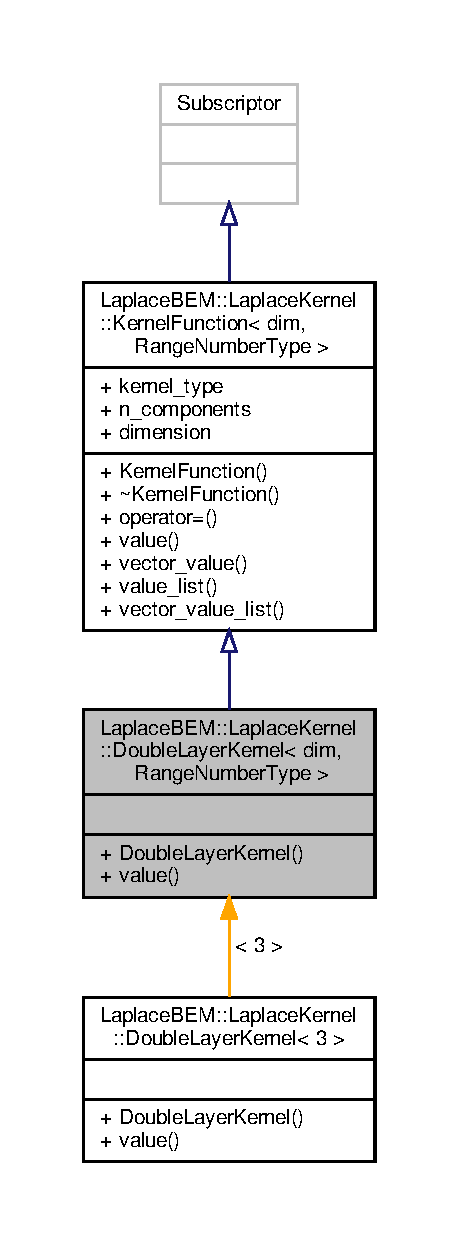
\includegraphics[height=550pt]{classLaplaceBEM_1_1LaplaceKernel_1_1DoubleLayerKernel__inherit__graph}
\end{center}
\end{figure}


Collaboration diagram for Laplace\+B\+EM\+:\+:Laplace\+Kernel\+:\+:Double\+Layer\+Kernel$<$ dim, Range\+Number\+Type $>$\+:\nopagebreak
\begin{figure}[H]
\begin{center}
\leavevmode
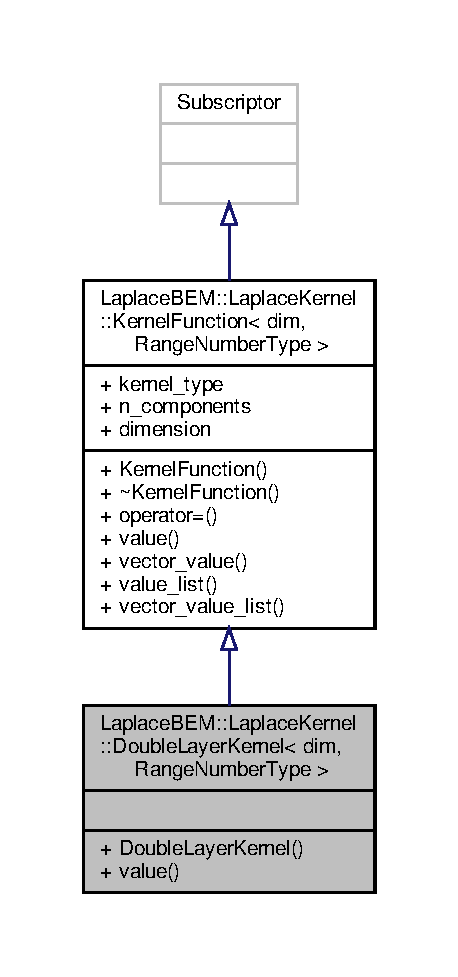
\includegraphics[width=220pt]{classLaplaceBEM_1_1LaplaceKernel_1_1DoubleLayerKernel__coll__graph}
\end{center}
\end{figure}
\subsection*{Public Member Functions}
\begin{DoxyCompactItemize}
\item 
\mbox{\Hypertarget{classLaplaceBEM_1_1LaplaceKernel_1_1DoubleLayerKernel_a44836d10e150f631a40d16dc2092fdad}\label{classLaplaceBEM_1_1LaplaceKernel_1_1DoubleLayerKernel_a44836d10e150f631a40d16dc2092fdad}} 
virtual Range\+Number\+Type {\bfseries value} (const Point$<$ dim $>$ \&x, const Point$<$ dim $>$ \&y, const Tensor$<$ 1, dim $>$ \&nx, const Tensor$<$ 1, dim $>$ \&ny, const unsigned int component=0) const override
\end{DoxyCompactItemize}
\subsection*{Additional Inherited Members}


\subsection{Detailed Description}
\subsubsection*{template$<$int dim, typename Range\+Number\+Type = double$>$\newline
class Laplace\+B\+E\+M\+::\+Laplace\+Kernel\+::\+Double\+Layer\+Kernel$<$ dim, Range\+Number\+Type $>$}

Double layer kernel. 

The documentation for this class was generated from the following file\+:\begin{DoxyCompactItemize}
\item 
/home/jihuan/\+Projects/deal.\+ii/program/dealii-\/9.\+1.\+1/examples/laplace-\/bem/include/\hyperlink{laplace__bem_8h}{laplace\+\_\+bem.\+h}\end{DoxyCompactItemize}

\hypertarget{classLaplaceBEM_1_1Erichsen1996Efficient_1_1Example2}{}\section{Laplace\+B\+EM\+:\+:Erichsen1996\+Efficient\+:\+:Example2 Class Reference}
\label{classLaplaceBEM_1_1Erichsen1996Efficient_1_1Example2}\index{Laplace\+B\+E\+M\+::\+Erichsen1996\+Efficient\+::\+Example2@{Laplace\+B\+E\+M\+::\+Erichsen1996\+Efficient\+::\+Example2}}


Collaboration diagram for Laplace\+B\+EM\+:\+:Erichsen1996\+Efficient\+:\+:Example2\+:\nopagebreak
\begin{figure}[H]
\begin{center}
\leavevmode
\includegraphics[height=550pt]{classLaplaceBEM_1_1Erichsen1996Efficient_1_1Example2__coll__graph}
\end{center}
\end{figure}
\subsection*{Classes}
\begin{DoxyCompactItemize}
\item 
class \hyperlink{classLaplaceBEM_1_1Erichsen1996Efficient_1_1Example2_1_1AnalyticalSolution}{Analytical\+Solution}
\item 
class \hyperlink{classLaplaceBEM_1_1Erichsen1996Efficient_1_1Example2_1_1NeumannBC}{Neumann\+BC}
\end{DoxyCompactItemize}
\subsection*{Public Member Functions}
\begin{DoxyCompactItemize}
\item 
\mbox{\Hypertarget{classLaplaceBEM_1_1Erichsen1996Efficient_1_1Example2_a174f958f5992499c541677385d3fd43b}\label{classLaplaceBEM_1_1Erichsen1996Efficient_1_1Example2_a174f958f5992499c541677385d3fd43b}} 
{\bfseries Example2} (const std\+::string \&mesh\+\_\+file\+\_\+name, unsigned int fe\+\_\+order=2)
\item 
\mbox{\Hypertarget{classLaplaceBEM_1_1Erichsen1996Efficient_1_1Example2_a05c16fcb30b3c88360ebd13a0e046c9e}\label{classLaplaceBEM_1_1Erichsen1996Efficient_1_1Example2_a05c16fcb30b3c88360ebd13a0e046c9e}} 
void {\bfseries run} ()
\item 
void \hyperlink{classLaplaceBEM_1_1Erichsen1996Efficient_1_1Example2_a4eda45fd98684daa5f951e74c27f0d84}{build\+\_\+slp\+\_\+only} (bool is\+\_\+build\+\_\+matrix)
\item 
\mbox{\Hypertarget{classLaplaceBEM_1_1Erichsen1996Efficient_1_1Example2_a77575ff8da117097f342daa9e949f9e5}\label{classLaplaceBEM_1_1Erichsen1996Efficient_1_1Example2_a77575ff8da117097f342daa9e949f9e5}} 
void {\bfseries output\+\_\+results} ()
\item 
\mbox{\Hypertarget{classLaplaceBEM_1_1Erichsen1996Efficient_1_1Example2_a34f1e4246d2330a0915890f0aef89447}\label{classLaplaceBEM_1_1Erichsen1996Efficient_1_1Example2_a34f1e4246d2330a0915890f0aef89447}} 
Full\+Matrix$<$ double $>$ \& {\bfseries get\+\_\+system\+\_\+matrix} ()
\item 
\mbox{\Hypertarget{classLaplaceBEM_1_1Erichsen1996Efficient_1_1Example2_aa29d813b54f41c70f187ae97b665e532}\label{classLaplaceBEM_1_1Erichsen1996Efficient_1_1Example2_aa29d813b54f41c70f187ae97b665e532}} 
Full\+Matrix$<$ double $>$ \& {\bfseries get\+\_\+system\+\_\+rhs\+\_\+slp\+\_\+matrix} ()
\item 
\mbox{\Hypertarget{classLaplaceBEM_1_1Erichsen1996Efficient_1_1Example2_a699c1e5eaa19496d464f3b9479489846}\label{classLaplaceBEM_1_1Erichsen1996Efficient_1_1Example2_a699c1e5eaa19496d464f3b9479489846}} 
Vector$<$ double $>$ \& {\bfseries get\+\_\+system\+\_\+rhs} ()
\item 
\mbox{\Hypertarget{classLaplaceBEM_1_1Erichsen1996Efficient_1_1Example2_a87cd1c586622395b63d85a0d93a59815}\label{classLaplaceBEM_1_1Erichsen1996Efficient_1_1Example2_a87cd1c586622395b63d85a0d93a59815}} 
\hyperlink{classClusterTree}{Cluster\+Tree}$<$ 3 $>$ \& {\bfseries get\+\_\+cluster\+\_\+tree} ()
\item 
\mbox{\Hypertarget{classLaplaceBEM_1_1Erichsen1996Efficient_1_1Example2_af712484fb8f5e371304c3e0f799e669e}\label{classLaplaceBEM_1_1Erichsen1996Efficient_1_1Example2_af712484fb8f5e371304c3e0f799e669e}} 
\hyperlink{classBlockClusterTree}{Block\+Cluster\+Tree}$<$ 3 $>$ \& {\bfseries get\+\_\+block\+\_\+cluster\+\_\+tree} ()
\end{DoxyCompactItemize}
\subsection*{Private Member Functions}
\begin{DoxyCompactItemize}
\item 
\mbox{\Hypertarget{classLaplaceBEM_1_1Erichsen1996Efficient_1_1Example2_a4771be3ff7c2e6308e13b3d21756ff1c}\label{classLaplaceBEM_1_1Erichsen1996Efficient_1_1Example2_a4771be3ff7c2e6308e13b3d21756ff1c}} 
void {\bfseries generate\+\_\+mesh} (unsigned int number\+\_\+of\+\_\+refinements=0)
\item 
void \hyperlink{classLaplaceBEM_1_1Erichsen1996Efficient_1_1Example2_a0d5abae56e8da05aad9ade216126109a}{read\+\_\+mesh} ()
\item 
void \hyperlink{classLaplaceBEM_1_1Erichsen1996Efficient_1_1Example2_a6a47dc2d39a4a3ff6b446e43e520bde7}{calc\+\_\+cell\+\_\+neighboring\+\_\+types} ()
\item 
void \hyperlink{classLaplaceBEM_1_1Erichsen1996Efficient_1_1Example2_a7bece202baddc2ff307f19d973f744fa}{setup\+\_\+system} ()
\item 
void \hyperlink{classLaplaceBEM_1_1Erichsen1996Efficient_1_1Example2_a8fd1e4be1faa412424e1ee521c597d37}{assemble\+\_\+on\+\_\+one\+\_\+cell} (const typename Do\+F\+Handler$<$ 2, 3 $>$\+::active\+\_\+cell\+\_\+iterator \&cell\+\_\+iter, \hyperlink{structLaplaceBEM_1_1CellWiseScratchData}{Cell\+Wise\+Scratch\+Data} \&scratch, \hyperlink{structLaplaceBEM_1_1CellWisePerTaskData}{Cell\+Wise\+Per\+Task\+Data} \&data)
\item 
void \hyperlink{classLaplaceBEM_1_1Erichsen1996Efficient_1_1Example2_aafff0bc1b7690a0150ba69991d37ef26}{copy\+\_\+cell\+\_\+local\+\_\+to\+\_\+global} (const \hyperlink{structLaplaceBEM_1_1CellWisePerTaskData}{Cell\+Wise\+Per\+Task\+Data} \&data)
\item 
void \hyperlink{classLaplaceBEM_1_1Erichsen1996Efficient_1_1Example2_afe943d5681aaef439208f51dc463f173}{assemble\+\_\+on\+\_\+one\+\_\+pair\+\_\+of\+\_\+cells} (const typename Do\+F\+Handler$<$ 2, 3 $>$\+::active\+\_\+cell\+\_\+iterator \&kx\+\_\+cell\+\_\+iter, const typename Do\+F\+Handler$<$ 2, 3 $>$\+::active\+\_\+cell\+\_\+iterator \&ky\+\_\+cell\+\_\+iter, const \hyperlink{classLaplaceBEM_1_1BEMValues}{B\+E\+M\+Values}$<$ 2, 3 $>$ \&bem\+\_\+values, \hyperlink{structLaplaceBEM_1_1PairCellWiseScratchData}{Pair\+Cell\+Wise\+Scratch\+Data} \&scratch, \hyperlink{structLaplaceBEM_1_1PairCellWisePerTaskData}{Pair\+Cell\+Wise\+Per\+Task\+Data} \&data)
\item 
\mbox{\Hypertarget{classLaplaceBEM_1_1Erichsen1996Efficient_1_1Example2_a9db729e8ccddf18dc156357679ea30e8}\label{classLaplaceBEM_1_1Erichsen1996Efficient_1_1Example2_a9db729e8ccddf18dc156357679ea30e8}} 
void {\bfseries assemble\+\_\+on\+\_\+one\+\_\+pair\+\_\+of\+\_\+cells\+\_\+for\+\_\+slp} (const typename Do\+F\+Handler$<$ 2, 3 $>$\+::active\+\_\+cell\+\_\+iterator \&kx\+\_\+cell\+\_\+iter, const typename Do\+F\+Handler$<$ 2, 3 $>$\+::active\+\_\+cell\+\_\+iterator \&ky\+\_\+cell\+\_\+iter, const \hyperlink{classLaplaceBEM_1_1BEMValues}{B\+E\+M\+Values}$<$ 2, 3 $>$ \&bem\+\_\+values, \hyperlink{structLaplaceBEM_1_1PairCellWiseScratchData}{Pair\+Cell\+Wise\+Scratch\+Data} \&scratch, \hyperlink{structLaplaceBEM_1_1PairCellWisePerTaskData}{Pair\+Cell\+Wise\+Per\+Task\+Data} \&data)
\item 
\mbox{\Hypertarget{classLaplaceBEM_1_1Erichsen1996Efficient_1_1Example2_a8844ffa9db41c840eb02dbb6eefed24d}\label{classLaplaceBEM_1_1Erichsen1996Efficient_1_1Example2_a8844ffa9db41c840eb02dbb6eefed24d}} 
void {\bfseries copy\+\_\+pair\+\_\+of\+\_\+cells\+\_\+local\+\_\+to\+\_\+global} (const \hyperlink{structLaplaceBEM_1_1PairCellWisePerTaskData}{Pair\+Cell\+Wise\+Per\+Task\+Data} \&data)
\item 
\mbox{\Hypertarget{classLaplaceBEM_1_1Erichsen1996Efficient_1_1Example2_a7ea82599971fb83e30322affa0606f55}\label{classLaplaceBEM_1_1Erichsen1996Efficient_1_1Example2_a7ea82599971fb83e30322affa0606f55}} 
void {\bfseries copy\+\_\+pair\+\_\+of\+\_\+cells\+\_\+local\+\_\+to\+\_\+global\+\_\+for\+\_\+slp} (const \hyperlink{structLaplaceBEM_1_1PairCellWisePerTaskData}{Pair\+Cell\+Wise\+Per\+Task\+Data} \&data)
\item 
\mbox{\Hypertarget{classLaplaceBEM_1_1Erichsen1996Efficient_1_1Example2_a316947cbda2c520f03d8a703e909380f}\label{classLaplaceBEM_1_1Erichsen1996Efficient_1_1Example2_a316947cbda2c520f03d8a703e909380f}} 
void {\bfseries assemble\+\_\+system\+\_\+smp} ()
\item 
void \hyperlink{classLaplaceBEM_1_1Erichsen1996Efficient_1_1Example2_a418130545bf95b1f331284810956d43e}{assemble\+\_\+slp\+\_\+smp} ()
\item 
void \hyperlink{classLaplaceBEM_1_1Erichsen1996Efficient_1_1Example2_a3e11e091f5fe741e19e72ad0cdc9c0c5}{assemble\+\_\+system\+\_\+serial} ()
\item 
\mbox{\Hypertarget{classLaplaceBEM_1_1Erichsen1996Efficient_1_1Example2_ae9e8baae33e3e331b84969b1315f0108}\label{classLaplaceBEM_1_1Erichsen1996Efficient_1_1Example2_ae9e8baae33e3e331b84969b1315f0108}} 
void {\bfseries solve} ()
\end{DoxyCompactItemize}
\subsection*{Private Attributes}
\begin{DoxyCompactItemize}
\item 
\mbox{\Hypertarget{classLaplaceBEM_1_1Erichsen1996Efficient_1_1Example2_a60a74b7651ab869be5e44d449f9c1428}\label{classLaplaceBEM_1_1Erichsen1996Efficient_1_1Example2_a60a74b7651ab869be5e44d449f9c1428}} 
std\+::string {\bfseries mesh\+\_\+file\+\_\+name}
\item 
\mbox{\Hypertarget{classLaplaceBEM_1_1Erichsen1996Efficient_1_1Example2_a8f8acf4d615ce67a0d89c4dc81aee4d1}\label{classLaplaceBEM_1_1Erichsen1996Efficient_1_1Example2_a8f8acf4d615ce67a0d89c4dc81aee4d1}} 
unsigned int {\bfseries fe\+\_\+order}
\item 
\mbox{\Hypertarget{classLaplaceBEM_1_1Erichsen1996Efficient_1_1Example2_a9733b849f670935fbfe76c36997f9b37}\label{classLaplaceBEM_1_1Erichsen1996Efficient_1_1Example2_a9733b849f670935fbfe76c36997f9b37}} 
Triangulation$<$ 2, 3 $>$ {\bfseries triangulation}
\item 
\mbox{\Hypertarget{classLaplaceBEM_1_1Erichsen1996Efficient_1_1Example2_a3e1f29510850246319dcc3b210bc9b98}\label{classLaplaceBEM_1_1Erichsen1996Efficient_1_1Example2_a3e1f29510850246319dcc3b210bc9b98}} 
F\+E\+\_\+Q$<$ 2, 3 $>$ {\bfseries fe}
\item 
\mbox{\Hypertarget{classLaplaceBEM_1_1Erichsen1996Efficient_1_1Example2_a15d25027f8e912cad3f7c523d0d702a7}\label{classLaplaceBEM_1_1Erichsen1996Efficient_1_1Example2_a15d25027f8e912cad3f7c523d0d702a7}} 
Do\+F\+Handler$<$ 2, 3 $>$ {\bfseries dof\+\_\+handler}
\item 
\mbox{\Hypertarget{classLaplaceBEM_1_1Erichsen1996Efficient_1_1Example2_ae0cf04215e1b81c7d0c105c02ece49ec}\label{classLaplaceBEM_1_1Erichsen1996Efficient_1_1Example2_ae0cf04215e1b81c7d0c105c02ece49ec}} 
Mapping\+Q\+Generic$<$ 2, 3 $>$ {\bfseries mapping}
\item 
\mbox{\Hypertarget{classLaplaceBEM_1_1Erichsen1996Efficient_1_1Example2_a6193afad812056811f0fbfa3b3a94a93}\label{classLaplaceBEM_1_1Erichsen1996Efficient_1_1Example2_a6193afad812056811f0fbfa3b3a94a93}} 
\hyperlink{classLaplaceBEM_1_1LaplaceKernel_1_1SingleLayerKernel}{Laplace\+Kernel\+::\+Single\+Layer\+Kernel}$<$ 3 $>$ {\bfseries slp}
\item 
\mbox{\Hypertarget{classLaplaceBEM_1_1Erichsen1996Efficient_1_1Example2_a6a1f162ff96662babfa5f5d47d85d2d8}\label{classLaplaceBEM_1_1Erichsen1996Efficient_1_1Example2_a6a1f162ff96662babfa5f5d47d85d2d8}} 
\hyperlink{classLaplaceBEM_1_1LaplaceKernel_1_1DoubleLayerKernel}{Laplace\+Kernel\+::\+Double\+Layer\+Kernel}$<$ 3 $>$ {\bfseries dlp}
\item 
\mbox{\Hypertarget{classLaplaceBEM_1_1Erichsen1996Efficient_1_1Example2_a32fdd8e2e8a8f815bb304a73da1b9713}\label{classLaplaceBEM_1_1Erichsen1996Efficient_1_1Example2_a32fdd8e2e8a8f815bb304a73da1b9713}} 
Point$<$ 3 $>$ {\bfseries x0}
\item 
\mbox{\Hypertarget{classLaplaceBEM_1_1Erichsen1996Efficient_1_1Example2_a72d0905d33d5f7bc1299809a21fe5a51}\label{classLaplaceBEM_1_1Erichsen1996Efficient_1_1Example2_a72d0905d33d5f7bc1299809a21fe5a51}} 
Point$<$ 3 $>$ {\bfseries model\+\_\+sphere\+\_\+center}
\item 
\mbox{\Hypertarget{classLaplaceBEM_1_1Erichsen1996Efficient_1_1Example2_a3ff5091415373a71bb59fcc6df159c81}\label{classLaplaceBEM_1_1Erichsen1996Efficient_1_1Example2_a3ff5091415373a71bb59fcc6df159c81}} 
double {\bfseries model\+\_\+sphere\+\_\+radius}
\item 
Full\+Matrix$<$ double $>$ \hyperlink{classLaplaceBEM_1_1Erichsen1996Efficient_1_1Example2_a9c76773c78cc3a09eb1f7e4f9d44d0c8}{system\+\_\+matrix}
\item 
Full\+Matrix$<$ double $>$ \hyperlink{classLaplaceBEM_1_1Erichsen1996Efficient_1_1Example2_a13e4add9320ecede8e53b7a633805740}{system\+\_\+rhs\+\_\+matrix}
\item 
Vector$<$ double $>$ \hyperlink{classLaplaceBEM_1_1Erichsen1996Efficient_1_1Example2_a52203aaab49947b16cf4f1a46f245375}{neumann\+\_\+bc}
\item 
Vector$<$ double $>$ \hyperlink{classLaplaceBEM_1_1Erichsen1996Efficient_1_1Example2_a7de5f9e1f110ec7f842577a54dddd267}{system\+\_\+rhs}
\item 
\mbox{\Hypertarget{classLaplaceBEM_1_1Erichsen1996Efficient_1_1Example2_a04c3a97e7c2a19636bcc3dcfe21f49b5}\label{classLaplaceBEM_1_1Erichsen1996Efficient_1_1Example2_a04c3a97e7c2a19636bcc3dcfe21f49b5}} 
Vector$<$ double $>$ {\bfseries analytical\+\_\+solution}
\item 
\mbox{\Hypertarget{classLaplaceBEM_1_1Erichsen1996Efficient_1_1Example2_a2cbc38adde4b9fdf2cd1bf322b046b6c}\label{classLaplaceBEM_1_1Erichsen1996Efficient_1_1Example2_a2cbc38adde4b9fdf2cd1bf322b046b6c}} 
Vector$<$ double $>$ {\bfseries solution}
\item 
std\+::vector$<$ types\+::global\+\_\+dof\+\_\+index $>$ \hyperlink{classLaplaceBEM_1_1Erichsen1996Efficient_1_1Example2_aeab9b4719f0dfe0086b51ce909f056fb}{dof\+\_\+indices}
\item 
std\+::vector$<$ Point$<$ 3 $>$ $>$ \hyperlink{classLaplaceBEM_1_1Erichsen1996Efficient_1_1Example2_a80f5db5e8f9f1705f4580d3005adbcef}{all\+\_\+support\+\_\+points}
\item 
std\+::vector$<$ double $>$ \hyperlink{classLaplaceBEM_1_1Erichsen1996Efficient_1_1Example2_a39146546262134939101501a5de42ab7}{dof\+\_\+average\+\_\+cell\+\_\+size}
\item 
\mbox{\Hypertarget{classLaplaceBEM_1_1Erichsen1996Efficient_1_1Example2_ac434cc1126b375fbc113d34cc4623fef}\label{classLaplaceBEM_1_1Erichsen1996Efficient_1_1Example2_ac434cc1126b375fbc113d34cc4623fef}} 
unsigned int {\bfseries n\+\_\+min\+\_\+for\+\_\+ct}
\item 
\mbox{\Hypertarget{classLaplaceBEM_1_1Erichsen1996Efficient_1_1Example2_a82b82c6c8852bf61b20a4e773853ef88}\label{classLaplaceBEM_1_1Erichsen1996Efficient_1_1Example2_a82b82c6c8852bf61b20a4e773853ef88}} 
double {\bfseries eta}
\item 
\mbox{\Hypertarget{classLaplaceBEM_1_1Erichsen1996Efficient_1_1Example2_a4f0541afa68eab38b9673cf89092ab91}\label{classLaplaceBEM_1_1Erichsen1996Efficient_1_1Example2_a4f0541afa68eab38b9673cf89092ab91}} 
\hyperlink{classClusterTree}{Cluster\+Tree}$<$ 3 $>$ {\bfseries ct}
\item 
\mbox{\Hypertarget{classLaplaceBEM_1_1Erichsen1996Efficient_1_1Example2_a618d3388cbc35b477216c8e321c5a176}\label{classLaplaceBEM_1_1Erichsen1996Efficient_1_1Example2_a618d3388cbc35b477216c8e321c5a176}} 
\hyperlink{classBlockClusterTree}{Block\+Cluster\+Tree}$<$ 3 $>$ {\bfseries bct}
\end{DoxyCompactItemize}


\subsection{Member Function Documentation}
\mbox{\Hypertarget{classLaplaceBEM_1_1Erichsen1996Efficient_1_1Example2_a8fd1e4be1faa412424e1ee521c597d37}\label{classLaplaceBEM_1_1Erichsen1996Efficient_1_1Example2_a8fd1e4be1faa412424e1ee521c597d37}} 
\index{Laplace\+B\+E\+M\+::\+Erichsen1996\+Efficient\+::\+Example2@{Laplace\+B\+E\+M\+::\+Erichsen1996\+Efficient\+::\+Example2}!assemble\+\_\+on\+\_\+one\+\_\+cell@{assemble\+\_\+on\+\_\+one\+\_\+cell}}
\index{assemble\+\_\+on\+\_\+one\+\_\+cell@{assemble\+\_\+on\+\_\+one\+\_\+cell}!Laplace\+B\+E\+M\+::\+Erichsen1996\+Efficient\+::\+Example2@{Laplace\+B\+E\+M\+::\+Erichsen1996\+Efficient\+::\+Example2}}
\subsubsection{\texorpdfstring{assemble\+\_\+on\+\_\+one\+\_\+cell()}{assemble\_on\_one\_cell()}}
{\footnotesize\ttfamily void Laplace\+B\+E\+M\+::\+Erichsen1996\+Efficient\+::\+Example2\+::assemble\+\_\+on\+\_\+one\+\_\+cell (\begin{DoxyParamCaption}\item[{const typename Do\+F\+Handler$<$ 2, 3 $>$\+::active\+\_\+cell\+\_\+iterator \&}]{cell\+\_\+iter,  }\item[{\hyperlink{structLaplaceBEM_1_1CellWiseScratchData}{Cell\+Wise\+Scratch\+Data} \&}]{scratch,  }\item[{\hyperlink{structLaplaceBEM_1_1CellWisePerTaskData}{Cell\+Wise\+Per\+Task\+Data} \&}]{data }\end{DoxyParamCaption})\hspace{0.3cm}{\ttfamily [private]}}

For handling F\+EM related cell wise integral.


\begin{DoxyParams}{Parameters}
{\em cell\+\_\+iter} & \\
\hline
{\em scratch} & \\
\hline
{\em data} & \\
\hline
\end{DoxyParams}
Clear the local matrix in case that it is reused from another finished task. N.\+B. Its memory has already been allocated in the constructor of {\ttfamily \hyperlink{structLaplaceBEM_1_1CellWisePerTaskData}{Cell\+Wise\+Per\+Task\+Data}}.\mbox{\Hypertarget{classLaplaceBEM_1_1Erichsen1996Efficient_1_1Example2_afe943d5681aaef439208f51dc463f173}\label{classLaplaceBEM_1_1Erichsen1996Efficient_1_1Example2_afe943d5681aaef439208f51dc463f173}} 
\index{Laplace\+B\+E\+M\+::\+Erichsen1996\+Efficient\+::\+Example2@{Laplace\+B\+E\+M\+::\+Erichsen1996\+Efficient\+::\+Example2}!assemble\+\_\+on\+\_\+one\+\_\+pair\+\_\+of\+\_\+cells@{assemble\+\_\+on\+\_\+one\+\_\+pair\+\_\+of\+\_\+cells}}
\index{assemble\+\_\+on\+\_\+one\+\_\+pair\+\_\+of\+\_\+cells@{assemble\+\_\+on\+\_\+one\+\_\+pair\+\_\+of\+\_\+cells}!Laplace\+B\+E\+M\+::\+Erichsen1996\+Efficient\+::\+Example2@{Laplace\+B\+E\+M\+::\+Erichsen1996\+Efficient\+::\+Example2}}
\subsubsection{\texorpdfstring{assemble\+\_\+on\+\_\+one\+\_\+pair\+\_\+of\+\_\+cells()}{assemble\_on\_one\_pair\_of\_cells()}}
{\footnotesize\ttfamily void Laplace\+B\+E\+M\+::\+Erichsen1996\+Efficient\+::\+Example2\+::assemble\+\_\+on\+\_\+one\+\_\+pair\+\_\+of\+\_\+cells (\begin{DoxyParamCaption}\item[{const typename Do\+F\+Handler$<$ 2, 3 $>$\+::active\+\_\+cell\+\_\+iterator \&}]{kx\+\_\+cell\+\_\+iter,  }\item[{const typename Do\+F\+Handler$<$ 2, 3 $>$\+::active\+\_\+cell\+\_\+iterator \&}]{ky\+\_\+cell\+\_\+iter,  }\item[{const \hyperlink{classLaplaceBEM_1_1BEMValues}{B\+E\+M\+Values}$<$ 2, 3 $>$ \&}]{bem\+\_\+values,  }\item[{\hyperlink{structLaplaceBEM_1_1PairCellWiseScratchData}{Pair\+Cell\+Wise\+Scratch\+Data} \&}]{scratch,  }\item[{\hyperlink{structLaplaceBEM_1_1PairCellWisePerTaskData}{Pair\+Cell\+Wise\+Per\+Task\+Data} \&}]{data }\end{DoxyParamCaption})\hspace{0.3cm}{\ttfamily [private]}}

Assemble B\+EM matrices on a pair of cells, i.\+e. $K_x$ as the field cell and $K_y$ as the source cell.


\begin{DoxyParams}{Parameters}
{\em kx\+\_\+cell\+\_\+iter} & \\
\hline
{\em ky\+\_\+cell\+\_\+iter} & \\
\hline
{\em scratch} & \\
\hline
{\em data} & \\
\hline
\end{DoxyParams}
Get support points in the lexicographic order.

Get permuted local DoF indices in the lexicographic order.

Select the quadrature rule.

Precalculate surface Jacobians and normal vectors at each quadrature point in the current pair of cells.

References Laplace\+B\+E\+M\+::get\+\_\+hierarchic\+\_\+support\+\_\+points\+\_\+in\+\_\+real\+\_\+cell(), Laplace\+B\+E\+M\+::\+Pair\+Cell\+Wise\+Scratch\+Data\+::kx\+\_\+local\+\_\+dof\+\_\+indices\+\_\+hierarchical, Laplace\+B\+E\+M\+::\+Pair\+Cell\+Wise\+Scratch\+Data\+::kx\+\_\+support\+\_\+points\+\_\+hierarchical, Laplace\+B\+E\+M\+::\+Pair\+Cell\+Wise\+Scratch\+Data\+::ky\+\_\+local\+\_\+dof\+\_\+indices\+\_\+hierarchical, Laplace\+B\+E\+M\+::\+Pair\+Cell\+Wise\+Scratch\+Data\+::ky\+\_\+support\+\_\+points\+\_\+hierarchical, and Laplace\+B\+E\+M\+::\+Pair\+Cell\+Wise\+Scratch\+Data\+::vertex\+\_\+dof\+\_\+index\+\_\+intersection.



Referenced by assemble\+\_\+slp\+\_\+smp().

\mbox{\Hypertarget{classLaplaceBEM_1_1Erichsen1996Efficient_1_1Example2_a418130545bf95b1f331284810956d43e}\label{classLaplaceBEM_1_1Erichsen1996Efficient_1_1Example2_a418130545bf95b1f331284810956d43e}} 
\index{Laplace\+B\+E\+M\+::\+Erichsen1996\+Efficient\+::\+Example2@{Laplace\+B\+E\+M\+::\+Erichsen1996\+Efficient\+::\+Example2}!assemble\+\_\+slp\+\_\+smp@{assemble\+\_\+slp\+\_\+smp}}
\index{assemble\+\_\+slp\+\_\+smp@{assemble\+\_\+slp\+\_\+smp}!Laplace\+B\+E\+M\+::\+Erichsen1996\+Efficient\+::\+Example2@{Laplace\+B\+E\+M\+::\+Erichsen1996\+Efficient\+::\+Example2}}
\subsubsection{\texorpdfstring{assemble\+\_\+slp\+\_\+smp()}{assemble\_slp\_smp()}}
{\footnotesize\ttfamily void Laplace\+B\+E\+M\+::\+Erichsen1996\+Efficient\+::\+Example2\+::assemble\+\_\+slp\+\_\+smp (\begin{DoxyParamCaption}{ }\end{DoxyParamCaption})\hspace{0.3cm}{\ttfamily [private]}}

Build S\+LP matrix only using S\+MP parallelization. 

References assemble\+\_\+on\+\_\+one\+\_\+pair\+\_\+of\+\_\+cells(), Laplace\+B\+E\+M\+::\+B\+E\+M\+Values$<$ dim, spacedim, Range\+Number\+Type $>$\+::fill\+\_\+shape\+\_\+grad\+\_\+matrix\+\_\+tables(), Laplace\+B\+E\+M\+::\+B\+E\+M\+Values$<$ dim, spacedim, Range\+Number\+Type $>$\+::fill\+\_\+shape\+\_\+value\+\_\+tables(), neumann\+\_\+bc, system\+\_\+rhs, and system\+\_\+rhs\+\_\+matrix.



Referenced by build\+\_\+slp\+\_\+only().

\mbox{\Hypertarget{classLaplaceBEM_1_1Erichsen1996Efficient_1_1Example2_a3e11e091f5fe741e19e72ad0cdc9c0c5}\label{classLaplaceBEM_1_1Erichsen1996Efficient_1_1Example2_a3e11e091f5fe741e19e72ad0cdc9c0c5}} 
\index{Laplace\+B\+E\+M\+::\+Erichsen1996\+Efficient\+::\+Example2@{Laplace\+B\+E\+M\+::\+Erichsen1996\+Efficient\+::\+Example2}!assemble\+\_\+system\+\_\+serial@{assemble\+\_\+system\+\_\+serial}}
\index{assemble\+\_\+system\+\_\+serial@{assemble\+\_\+system\+\_\+serial}!Laplace\+B\+E\+M\+::\+Erichsen1996\+Efficient\+::\+Example2@{Laplace\+B\+E\+M\+::\+Erichsen1996\+Efficient\+::\+Example2}}
\subsubsection{\texorpdfstring{assemble\+\_\+system\+\_\+serial()}{assemble\_system\_serial()}}
{\footnotesize\ttfamily void Laplace\+B\+E\+M\+::\+Erichsen1996\+Efficient\+::\+Example2\+::assemble\+\_\+system\+\_\+serial (\begin{DoxyParamCaption}{ }\end{DoxyParamCaption})\hspace{0.3cm}{\ttfamily [private]}}

Precalculate shape function values and their gradient values at each quadrature point. N.\+B.


\begin{DoxyEnumerate}
\item The data tables for shape function values and their gradient values should be calculated for both function space on $K_x$ and function space on $K_y$.
\item Being different from the integral in F\+EM, the integral in Galerkin-\/\+B\+EM handled by Sauter\textquotesingle{}s quadrature rule has multiple parts of $k_3$ (except the regular cell neighboring type), each of which should be evaluated at a different set of quadrature points in the unit cell after coordinate transformation from the parametric space. Therefore, a dimension with respect to $k_3$ term index should be added to the data table compared to the usual {\ttfamily F\+E\+Values}.
\end{DoxyEnumerate}

References calc\+\_\+cell\+\_\+neighboring\+\_\+types(), Laplace\+B\+E\+M\+::\+B\+E\+M\+Values$<$ dim, spacedim, Range\+Number\+Type $>$\+::fill\+\_\+shape\+\_\+grad\+\_\+matrix\+\_\+tables(), Laplace\+B\+E\+M\+::\+B\+E\+M\+Values$<$ dim, spacedim, Range\+Number\+Type $>$\+::fill\+\_\+shape\+\_\+value\+\_\+tables(), neumann\+\_\+bc, read\+\_\+mesh(), setup\+\_\+system(), system\+\_\+matrix, system\+\_\+rhs, and system\+\_\+rhs\+\_\+matrix.



Referenced by build\+\_\+slp\+\_\+only().

\mbox{\Hypertarget{classLaplaceBEM_1_1Erichsen1996Efficient_1_1Example2_a4eda45fd98684daa5f951e74c27f0d84}\label{classLaplaceBEM_1_1Erichsen1996Efficient_1_1Example2_a4eda45fd98684daa5f951e74c27f0d84}} 
\index{Laplace\+B\+E\+M\+::\+Erichsen1996\+Efficient\+::\+Example2@{Laplace\+B\+E\+M\+::\+Erichsen1996\+Efficient\+::\+Example2}!build\+\_\+slp\+\_\+only@{build\+\_\+slp\+\_\+only}}
\index{build\+\_\+slp\+\_\+only@{build\+\_\+slp\+\_\+only}!Laplace\+B\+E\+M\+::\+Erichsen1996\+Efficient\+::\+Example2@{Laplace\+B\+E\+M\+::\+Erichsen1996\+Efficient\+::\+Example2}}
\subsubsection{\texorpdfstring{build\+\_\+slp\+\_\+only()}{build\_slp\_only()}}
{\footnotesize\ttfamily void Laplace\+B\+E\+M\+::\+Erichsen1996\+Efficient\+::\+Example2\+::build\+\_\+slp\+\_\+only (\begin{DoxyParamCaption}\item[{bool}]{is\+\_\+build\+\_\+matrix }\end{DoxyParamCaption})}

Generate the sequence of all DoF indices with the values $0, 1, \cdots$.

Get the spatial coordinates of the support points associated with DoF indices. The used {\ttfamily mapping} object here should be consistent with the Finte\+Element space adopted.

Calculate the distance between each pair of support points associated with Do\+Fs.

Calculate the average mesh cell size at each support point.

Create the cluster tree.

Create the block cluster tree.

References all\+\_\+support\+\_\+points, assemble\+\_\+slp\+\_\+smp(), assemble\+\_\+system\+\_\+serial(), calc\+\_\+cell\+\_\+neighboring\+\_\+types(), dof\+\_\+average\+\_\+cell\+\_\+size, dof\+\_\+indices, map\+\_\+dofs\+\_\+to\+\_\+average\+\_\+cell\+\_\+size(), Cluster\+Tree$<$ spacedim, Number $>$\+::partition(), Block\+Cluster\+Tree$<$ spacedim, Number $>$\+::partition(), read\+\_\+mesh(), and setup\+\_\+system().



Referenced by main().

\mbox{\Hypertarget{classLaplaceBEM_1_1Erichsen1996Efficient_1_1Example2_a6a47dc2d39a4a3ff6b446e43e520bde7}\label{classLaplaceBEM_1_1Erichsen1996Efficient_1_1Example2_a6a47dc2d39a4a3ff6b446e43e520bde7}} 
\index{Laplace\+B\+E\+M\+::\+Erichsen1996\+Efficient\+::\+Example2@{Laplace\+B\+E\+M\+::\+Erichsen1996\+Efficient\+::\+Example2}!calc\+\_\+cell\+\_\+neighboring\+\_\+types@{calc\+\_\+cell\+\_\+neighboring\+\_\+types}}
\index{calc\+\_\+cell\+\_\+neighboring\+\_\+types@{calc\+\_\+cell\+\_\+neighboring\+\_\+types}!Laplace\+B\+E\+M\+::\+Erichsen1996\+Efficient\+::\+Example2@{Laplace\+B\+E\+M\+::\+Erichsen1996\+Efficient\+::\+Example2}}
\subsubsection{\texorpdfstring{calc\+\_\+cell\+\_\+neighboring\+\_\+types()}{calc\_cell\_neighboring\_types()}}
{\footnotesize\ttfamily void Laplace\+B\+E\+M\+::\+Erichsen1996\+Efficient\+::\+Example2\+::calc\+\_\+cell\+\_\+neighboring\+\_\+types (\begin{DoxyParamCaption}{ }\end{DoxyParamCaption})\hspace{0.3cm}{\ttfamily [private]}}

Calculate the neighboring type for each pair of cells. 

Referenced by assemble\+\_\+system\+\_\+serial(), and build\+\_\+slp\+\_\+only().

\mbox{\Hypertarget{classLaplaceBEM_1_1Erichsen1996Efficient_1_1Example2_aafff0bc1b7690a0150ba69991d37ef26}\label{classLaplaceBEM_1_1Erichsen1996Efficient_1_1Example2_aafff0bc1b7690a0150ba69991d37ef26}} 
\index{Laplace\+B\+E\+M\+::\+Erichsen1996\+Efficient\+::\+Example2@{Laplace\+B\+E\+M\+::\+Erichsen1996\+Efficient\+::\+Example2}!copy\+\_\+cell\+\_\+local\+\_\+to\+\_\+global@{copy\+\_\+cell\+\_\+local\+\_\+to\+\_\+global}}
\index{copy\+\_\+cell\+\_\+local\+\_\+to\+\_\+global@{copy\+\_\+cell\+\_\+local\+\_\+to\+\_\+global}!Laplace\+B\+E\+M\+::\+Erichsen1996\+Efficient\+::\+Example2@{Laplace\+B\+E\+M\+::\+Erichsen1996\+Efficient\+::\+Example2}}
\subsubsection{\texorpdfstring{copy\+\_\+cell\+\_\+local\+\_\+to\+\_\+global()}{copy\_cell\_local\_to\_global()}}
{\footnotesize\ttfamily void Laplace\+B\+E\+M\+::\+Erichsen1996\+Efficient\+::\+Example2\+::copy\+\_\+cell\+\_\+local\+\_\+to\+\_\+global (\begin{DoxyParamCaption}\item[{const \hyperlink{structLaplaceBEM_1_1CellWisePerTaskData}{Cell\+Wise\+Per\+Task\+Data} \&}]{data }\end{DoxyParamCaption})\hspace{0.3cm}{\ttfamily [private]}}

For handling F\+EM related cell wise matrix assembly.


\begin{DoxyParams}{Parameters}
{\em data} & \\
\hline
\end{DoxyParams}


References system\+\_\+matrix.

\mbox{\Hypertarget{classLaplaceBEM_1_1Erichsen1996Efficient_1_1Example2_a0d5abae56e8da05aad9ade216126109a}\label{classLaplaceBEM_1_1Erichsen1996Efficient_1_1Example2_a0d5abae56e8da05aad9ade216126109a}} 
\index{Laplace\+B\+E\+M\+::\+Erichsen1996\+Efficient\+::\+Example2@{Laplace\+B\+E\+M\+::\+Erichsen1996\+Efficient\+::\+Example2}!read\+\_\+mesh@{read\+\_\+mesh}}
\index{read\+\_\+mesh@{read\+\_\+mesh}!Laplace\+B\+E\+M\+::\+Erichsen1996\+Efficient\+::\+Example2@{Laplace\+B\+E\+M\+::\+Erichsen1996\+Efficient\+::\+Example2}}
\subsubsection{\texorpdfstring{read\+\_\+mesh()}{read\_mesh()}}
{\footnotesize\ttfamily void Laplace\+B\+E\+M\+::\+Erichsen1996\+Efficient\+::\+Example2\+::read\+\_\+mesh (\begin{DoxyParamCaption}{ }\end{DoxyParamCaption})\hspace{0.3cm}{\ttfamily [private]}}

Read the mesh from a file, which abandons the manifold description. 

Referenced by assemble\+\_\+system\+\_\+serial(), and build\+\_\+slp\+\_\+only().

\mbox{\Hypertarget{classLaplaceBEM_1_1Erichsen1996Efficient_1_1Example2_a7bece202baddc2ff307f19d973f744fa}\label{classLaplaceBEM_1_1Erichsen1996Efficient_1_1Example2_a7bece202baddc2ff307f19d973f744fa}} 
\index{Laplace\+B\+E\+M\+::\+Erichsen1996\+Efficient\+::\+Example2@{Laplace\+B\+E\+M\+::\+Erichsen1996\+Efficient\+::\+Example2}!setup\+\_\+system@{setup\+\_\+system}}
\index{setup\+\_\+system@{setup\+\_\+system}!Laplace\+B\+E\+M\+::\+Erichsen1996\+Efficient\+::\+Example2@{Laplace\+B\+E\+M\+::\+Erichsen1996\+Efficient\+::\+Example2}}
\subsubsection{\texorpdfstring{setup\+\_\+system()}{setup\_system()}}
{\footnotesize\ttfamily void Laplace\+B\+E\+M\+::\+Erichsen1996\+Efficient\+::\+Example2\+::setup\+\_\+system (\begin{DoxyParamCaption}{ }\end{DoxyParamCaption})\hspace{0.3cm}{\ttfamily [private]}}


\begin{DoxyDescription}
\item[Note ]Because {\ttfamily dof\+\_\+handler} is associated with both the Finite\+Element and the Triangulation, the following interpolation operation is feasible. 
\end{DoxyDescription}

References neumann\+\_\+bc, system\+\_\+matrix, system\+\_\+rhs, and system\+\_\+rhs\+\_\+matrix.



Referenced by assemble\+\_\+system\+\_\+serial(), and build\+\_\+slp\+\_\+only().



\subsection{Member Data Documentation}
\mbox{\Hypertarget{classLaplaceBEM_1_1Erichsen1996Efficient_1_1Example2_a80f5db5e8f9f1705f4580d3005adbcef}\label{classLaplaceBEM_1_1Erichsen1996Efficient_1_1Example2_a80f5db5e8f9f1705f4580d3005adbcef}} 
\index{Laplace\+B\+E\+M\+::\+Erichsen1996\+Efficient\+::\+Example2@{Laplace\+B\+E\+M\+::\+Erichsen1996\+Efficient\+::\+Example2}!all\+\_\+support\+\_\+points@{all\+\_\+support\+\_\+points}}
\index{all\+\_\+support\+\_\+points@{all\+\_\+support\+\_\+points}!Laplace\+B\+E\+M\+::\+Erichsen1996\+Efficient\+::\+Example2@{Laplace\+B\+E\+M\+::\+Erichsen1996\+Efficient\+::\+Example2}}
\subsubsection{\texorpdfstring{all\+\_\+support\+\_\+points}{all\_support\_points}}
{\footnotesize\ttfamily std\+::vector$<$Point$<$3$>$ $>$ Laplace\+B\+E\+M\+::\+Erichsen1996\+Efficient\+::\+Example2\+::all\+\_\+support\+\_\+points\hspace{0.3cm}{\ttfamily [private]}}

The list of all support points associated with {\ttfamily dof\+\_\+indices}. 

Referenced by build\+\_\+slp\+\_\+only().

\mbox{\Hypertarget{classLaplaceBEM_1_1Erichsen1996Efficient_1_1Example2_a39146546262134939101501a5de42ab7}\label{classLaplaceBEM_1_1Erichsen1996Efficient_1_1Example2_a39146546262134939101501a5de42ab7}} 
\index{Laplace\+B\+E\+M\+::\+Erichsen1996\+Efficient\+::\+Example2@{Laplace\+B\+E\+M\+::\+Erichsen1996\+Efficient\+::\+Example2}!dof\+\_\+average\+\_\+cell\+\_\+size@{dof\+\_\+average\+\_\+cell\+\_\+size}}
\index{dof\+\_\+average\+\_\+cell\+\_\+size@{dof\+\_\+average\+\_\+cell\+\_\+size}!Laplace\+B\+E\+M\+::\+Erichsen1996\+Efficient\+::\+Example2@{Laplace\+B\+E\+M\+::\+Erichsen1996\+Efficient\+::\+Example2}}
\subsubsection{\texorpdfstring{dof\+\_\+average\+\_\+cell\+\_\+size}{dof\_average\_cell\_size}}
{\footnotesize\ttfamily std\+::vector$<$double$>$ Laplace\+B\+E\+M\+::\+Erichsen1996\+Efficient\+::\+Example2\+::dof\+\_\+average\+\_\+cell\+\_\+size\hspace{0.3cm}{\ttfamily [private]}}

Estimated average cell size values associated with {\ttfamily dof\+\_\+indices}. 

Referenced by build\+\_\+slp\+\_\+only().

\mbox{\Hypertarget{classLaplaceBEM_1_1Erichsen1996Efficient_1_1Example2_aeab9b4719f0dfe0086b51ce909f056fb}\label{classLaplaceBEM_1_1Erichsen1996Efficient_1_1Example2_aeab9b4719f0dfe0086b51ce909f056fb}} 
\index{Laplace\+B\+E\+M\+::\+Erichsen1996\+Efficient\+::\+Example2@{Laplace\+B\+E\+M\+::\+Erichsen1996\+Efficient\+::\+Example2}!dof\+\_\+indices@{dof\+\_\+indices}}
\index{dof\+\_\+indices@{dof\+\_\+indices}!Laplace\+B\+E\+M\+::\+Erichsen1996\+Efficient\+::\+Example2@{Laplace\+B\+E\+M\+::\+Erichsen1996\+Efficient\+::\+Example2}}
\subsubsection{\texorpdfstring{dof\+\_\+indices}{dof\_indices}}
{\footnotesize\ttfamily std\+::vector$<$types\+::global\+\_\+dof\+\_\+index$>$ Laplace\+B\+E\+M\+::\+Erichsen1996\+Efficient\+::\+Example2\+::dof\+\_\+indices\hspace{0.3cm}{\ttfamily [private]}}

The sequence of all DoF indices with the values $0, 1, \cdots$. 

Referenced by build\+\_\+slp\+\_\+only().

\mbox{\Hypertarget{classLaplaceBEM_1_1Erichsen1996Efficient_1_1Example2_a52203aaab49947b16cf4f1a46f245375}\label{classLaplaceBEM_1_1Erichsen1996Efficient_1_1Example2_a52203aaab49947b16cf4f1a46f245375}} 
\index{Laplace\+B\+E\+M\+::\+Erichsen1996\+Efficient\+::\+Example2@{Laplace\+B\+E\+M\+::\+Erichsen1996\+Efficient\+::\+Example2}!neumann\+\_\+bc@{neumann\+\_\+bc}}
\index{neumann\+\_\+bc@{neumann\+\_\+bc}!Laplace\+B\+E\+M\+::\+Erichsen1996\+Efficient\+::\+Example2@{Laplace\+B\+E\+M\+::\+Erichsen1996\+Efficient\+::\+Example2}}
\subsubsection{\texorpdfstring{neumann\+\_\+bc}{neumann\_bc}}
{\footnotesize\ttfamily Vector$<$double$>$ Laplace\+B\+E\+M\+::\+Erichsen1996\+Efficient\+::\+Example2\+::neumann\+\_\+bc\hspace{0.3cm}{\ttfamily [private]}}

Neumann boundary condition data at each DoF support point. 

Referenced by assemble\+\_\+slp\+\_\+smp(), assemble\+\_\+system\+\_\+serial(), and setup\+\_\+system().

\mbox{\Hypertarget{classLaplaceBEM_1_1Erichsen1996Efficient_1_1Example2_a9c76773c78cc3a09eb1f7e4f9d44d0c8}\label{classLaplaceBEM_1_1Erichsen1996Efficient_1_1Example2_a9c76773c78cc3a09eb1f7e4f9d44d0c8}} 
\index{Laplace\+B\+E\+M\+::\+Erichsen1996\+Efficient\+::\+Example2@{Laplace\+B\+E\+M\+::\+Erichsen1996\+Efficient\+::\+Example2}!system\+\_\+matrix@{system\+\_\+matrix}}
\index{system\+\_\+matrix@{system\+\_\+matrix}!Laplace\+B\+E\+M\+::\+Erichsen1996\+Efficient\+::\+Example2@{Laplace\+B\+E\+M\+::\+Erichsen1996\+Efficient\+::\+Example2}}
\subsubsection{\texorpdfstring{system\+\_\+matrix}{system\_matrix}}
{\footnotesize\ttfamily Full\+Matrix$<$double$>$ Laplace\+B\+E\+M\+::\+Erichsen1996\+Efficient\+::\+Example2\+::system\+\_\+matrix\hspace{0.3cm}{\ttfamily [private]}}

System matrix obtained from \$(v, \{1\}\{2\}u) + (v, Ku)\$. The first integral term in the sum is carried on each cell, while the second integral term is carried out on each pair of cells. 

Referenced by assemble\+\_\+system\+\_\+serial(), copy\+\_\+cell\+\_\+local\+\_\+to\+\_\+global(), and setup\+\_\+system().

\mbox{\Hypertarget{classLaplaceBEM_1_1Erichsen1996Efficient_1_1Example2_a7de5f9e1f110ec7f842577a54dddd267}\label{classLaplaceBEM_1_1Erichsen1996Efficient_1_1Example2_a7de5f9e1f110ec7f842577a54dddd267}} 
\index{Laplace\+B\+E\+M\+::\+Erichsen1996\+Efficient\+::\+Example2@{Laplace\+B\+E\+M\+::\+Erichsen1996\+Efficient\+::\+Example2}!system\+\_\+rhs@{system\+\_\+rhs}}
\index{system\+\_\+rhs@{system\+\_\+rhs}!Laplace\+B\+E\+M\+::\+Erichsen1996\+Efficient\+::\+Example2@{Laplace\+B\+E\+M\+::\+Erichsen1996\+Efficient\+::\+Example2}}
\subsubsection{\texorpdfstring{system\+\_\+rhs}{system\_rhs}}
{\footnotesize\ttfamily Vector$<$double$>$ Laplace\+B\+E\+M\+::\+Erichsen1996\+Efficient\+::\+Example2\+::system\+\_\+rhs\hspace{0.3cm}{\ttfamily [private]}}

Right hand side vector for the problem obtained from the product of {\ttfamily system\+\_\+rhs\+\_\+matrix} and {\ttfamily neumann\+\_\+bc} 

Referenced by assemble\+\_\+slp\+\_\+smp(), assemble\+\_\+system\+\_\+serial(), and setup\+\_\+system().

\mbox{\Hypertarget{classLaplaceBEM_1_1Erichsen1996Efficient_1_1Example2_a13e4add9320ecede8e53b7a633805740}\label{classLaplaceBEM_1_1Erichsen1996Efficient_1_1Example2_a13e4add9320ecede8e53b7a633805740}} 
\index{Laplace\+B\+E\+M\+::\+Erichsen1996\+Efficient\+::\+Example2@{Laplace\+B\+E\+M\+::\+Erichsen1996\+Efficient\+::\+Example2}!system\+\_\+rhs\+\_\+matrix@{system\+\_\+rhs\+\_\+matrix}}
\index{system\+\_\+rhs\+\_\+matrix@{system\+\_\+rhs\+\_\+matrix}!Laplace\+B\+E\+M\+::\+Erichsen1996\+Efficient\+::\+Example2@{Laplace\+B\+E\+M\+::\+Erichsen1996\+Efficient\+::\+Example2}}
\subsubsection{\texorpdfstring{system\+\_\+rhs\+\_\+matrix}{system\_rhs\_matrix}}
{\footnotesize\ttfamily Full\+Matrix$<$double$>$ Laplace\+B\+E\+M\+::\+Erichsen1996\+Efficient\+::\+Example2\+::system\+\_\+rhs\+\_\+matrix\hspace{0.3cm}{\ttfamily [private]}}

The right hand side matrix obtained from \$(v, Vu)\$. 

Referenced by assemble\+\_\+slp\+\_\+smp(), assemble\+\_\+system\+\_\+serial(), and setup\+\_\+system().



The documentation for this class was generated from the following file\+:\begin{DoxyCompactItemize}
\item 
/home/jihuan/\+Projects/deal.\+ii/program/dealii-\/9.\+1.\+1/examples/laplace-\/bem/include/erichsen1996efficient\+\_\+example2.\+h\end{DoxyCompactItemize}

\hypertarget{classHMatrix}{}\section{H\+Matrix$<$ spacedim, Number $>$ Class Template Reference}
\label{classHMatrix}\index{H\+Matrix$<$ spacedim, Number $>$@{H\+Matrix$<$ spacedim, Number $>$}}


Collaboration diagram for H\+Matrix$<$ spacedim, Number $>$\+:\nopagebreak
\begin{figure}[H]
\begin{center}
\leavevmode
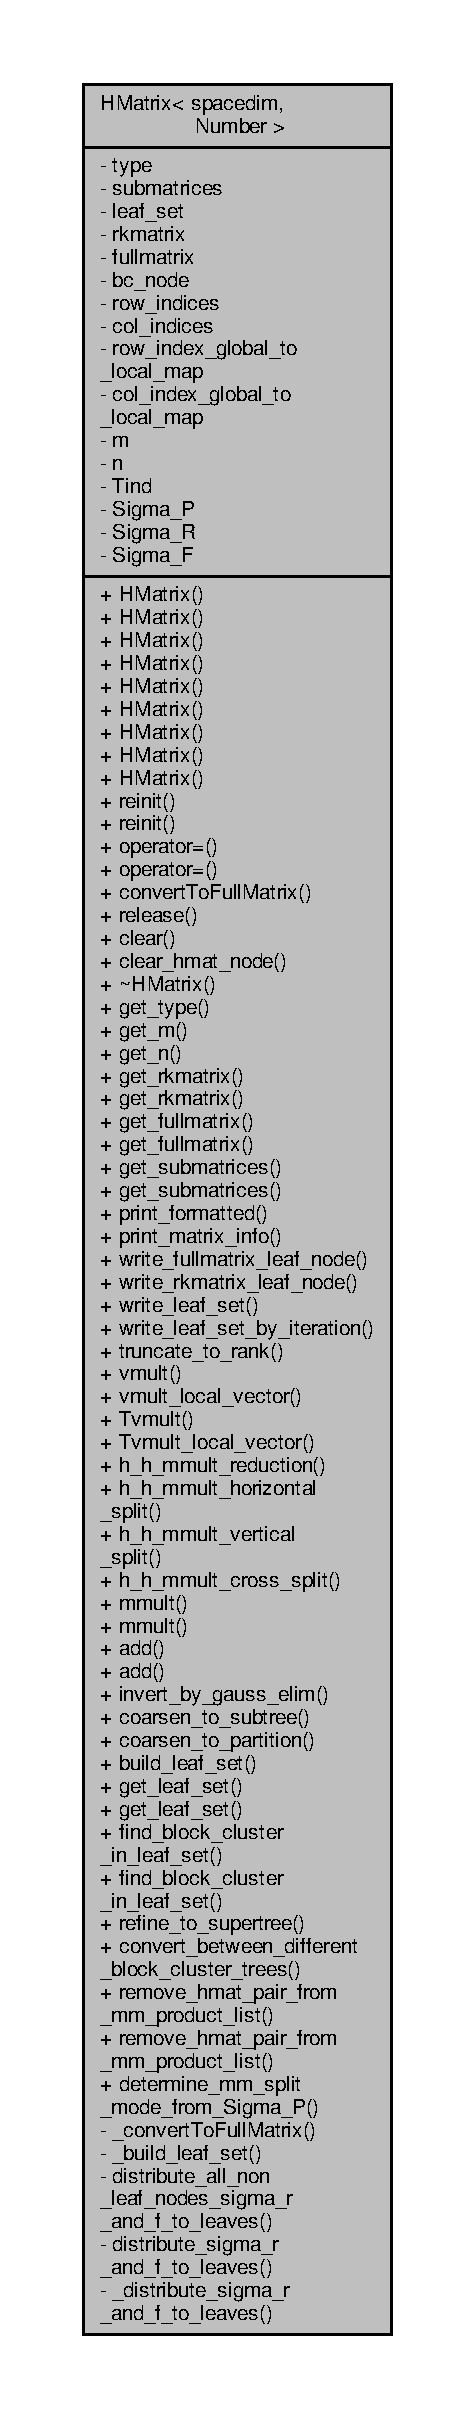
\includegraphics[height=550pt]{classHMatrix__coll__graph}
\end{center}
\end{figure}
\subsection*{Public Types}
\begin{DoxyCompactItemize}
\item 
using \hyperlink{classHMatrix_a5ca8dc549783d38371a01ecd621ecb34}{size\+\_\+type} = std\+::make\+\_\+unsigned$<$ types\+::blas\+\_\+int $>$\+::\hyperlink{classHMatrix_a89ef60f3ba737c04708195ca0bb13620}{type}
\end{DoxyCompactItemize}
\subsection*{Public Member Functions}
\begin{DoxyCompactItemize}
\item 
\hyperlink{classHMatrix_ae3dc35e1aefee2580d27ad2d65c906de}{H\+Matrix} ()
\item 
\hyperlink{classHMatrix_a6a4dead0321e8df38865bf6fbd0f6e81}{H\+Matrix} (const \hyperlink{classBlockClusterTree}{Block\+Cluster\+Tree}$<$ spacedim, Number $>$ \&bct, const unsigned int fixed\+\_\+rank\+\_\+k=1)
\item 
\hyperlink{classHMatrix_a4fe44a3aa2b813f593b787f24be56a1c}{H\+Matrix} (typename \hyperlink{classBlockClusterTree}{Block\+Cluster\+Tree}$<$ spacedim, Number $>$\+::node\+\_\+const\+\_\+pointer\+\_\+type \hyperlink{classHMatrix_a4a304494c970b5b267be1d8459d51586}{bc\+\_\+node}, const unsigned int fixed\+\_\+rank\+\_\+k=1)
\item 
\hyperlink{classHMatrix_a8e7d103ec4f093870f9e792e26d6b915}{H\+Matrix} (const \hyperlink{classBlockClusterTree}{Block\+Cluster\+Tree}$<$ spacedim, Number $>$ \&bct, const \hyperlink{classLAPACKFullMatrixExt}{L\+A\+P\+A\+C\+K\+Full\+Matrix\+Ext}$<$ Number $>$ \&M, const unsigned int fixed\+\_\+rank\+\_\+k=1)
\item 
\hyperlink{classHMatrix_abb59b3981e9f32f319479088d786989d}{H\+Matrix} (typename \hyperlink{classBlockClusterTree}{Block\+Cluster\+Tree}$<$ spacedim, Number $>$\+::node\+\_\+const\+\_\+pointer\+\_\+type \hyperlink{classHMatrix_a4a304494c970b5b267be1d8459d51586}{bc\+\_\+node}, const \hyperlink{classLAPACKFullMatrixExt}{L\+A\+P\+A\+C\+K\+Full\+Matrix\+Ext}$<$ Number $>$ \&M, const unsigned int fixed\+\_\+rank\+\_\+k=1)
\item 
\hyperlink{classHMatrix_abeb8d0add9bffecafc12f4c6b1dcab8e}{H\+Matrix} (typename \hyperlink{classBlockClusterTree}{Block\+Cluster\+Tree}$<$ spacedim, Number $>$\+::node\+\_\+const\+\_\+pointer\+\_\+type \hyperlink{classHMatrix_a4a304494c970b5b267be1d8459d51586}{bc\+\_\+node}, \hyperlink{classHMatrix}{H\+Matrix}$<$ spacedim, Number $>$ \&\&H)
\item 
\hyperlink{classHMatrix_a78aa967d7a99e27cc172f0db3791306b}{H\+Matrix} (const \hyperlink{classBlockClusterTree}{Block\+Cluster\+Tree}$<$ spacedim, Number $>$ \&bct, \hyperlink{classHMatrix}{H\+Matrix}$<$ spacedim, Number $>$ \&\&H)
\item 
\hyperlink{classHMatrix_a0b5227e35290f6c9fba1e8948e9a29c3}{H\+Matrix} (const \hyperlink{classHMatrix}{H\+Matrix}$<$ spacedim, Number $>$ \&H)
\item 
\hyperlink{classHMatrix_a556325d4cdaee699f17aa1be63bb58ee}{H\+Matrix} (\hyperlink{classHMatrix}{H\+Matrix}$<$ spacedim, Number $>$ \&\&H)
\item 
void \hyperlink{classHMatrix_a83f804163e1695cfb952ddb6b0df2503}{reinit} (const \hyperlink{classBlockClusterTree}{Block\+Cluster\+Tree}$<$ spacedim, Number $>$ \&bct, const unsigned int fixed\+\_\+rank\+\_\+k=1)
\item 
void \hyperlink{classHMatrix_a41d20c1839f3d7a756107b8e4defea0b}{reinit} (typename \hyperlink{classBlockClusterTree}{Block\+Cluster\+Tree}$<$ spacedim, Number $>$\+::node\+\_\+const\+\_\+pointer\+\_\+type \hyperlink{classHMatrix_a4a304494c970b5b267be1d8459d51586}{bc\+\_\+node}, const unsigned int fixed\+\_\+rank\+\_\+k=1)
\item 
\hyperlink{classHMatrix}{H\+Matrix}$<$ spacedim, Number $>$ \& \hyperlink{classHMatrix_a2c72ede65323af5b57a6b16f5774de50}{operator=} (\hyperlink{classHMatrix}{H\+Matrix}$<$ spacedim, Number $>$ \&\&H)
\item 
\hyperlink{classHMatrix}{H\+Matrix}$<$ spacedim, Number $>$ \& \hyperlink{classHMatrix_a83958971f40409b3b2a192b71eae1513}{operator=} (const \hyperlink{classHMatrix}{H\+Matrix}$<$ spacedim, Number $>$ \&H)
\item 
{\footnotesize template$<$typename Matrix\+Type $>$ }\\void \hyperlink{classHMatrix_a00bdd40f7fcf5c912c34c427df518300}{convert\+To\+Full\+Matrix} (Matrix\+Type \&M) const
\item 
void \hyperlink{classHMatrix_a812e8276888b2ad866edf7ce9b286839}{release} ()
\item 
void \hyperlink{classHMatrix_ae55bd45587b895bfdb977e7cbea46519}{clear} ()
\item 
void \hyperlink{classHMatrix_aec0815bc9c3654391bb2b3095383e6cb}{clear\+\_\+hmat\+\_\+node} ()
\item 
\hyperlink{classHMatrix_ae16c956c1b22eb307e9f360a83f4fa75}{$\sim$\+H\+Matrix} ()
\item 
\hyperlink{hmatrix_8h_ac04719e202c88f36e4533fe1d326a494}{H\+Matrix\+Type} \hyperlink{classHMatrix_aadea9fa59f420d22b3b1c939f6b573cc}{get\+\_\+type} () const
\item 
\hyperlink{classHMatrix_a5ca8dc549783d38371a01ecd621ecb34}{size\+\_\+type} \hyperlink{classHMatrix_aabe735f7712a10ba5325ff116f8ca1c7}{get\+\_\+m} () const
\item 
\hyperlink{classHMatrix_a5ca8dc549783d38371a01ecd621ecb34}{size\+\_\+type} \hyperlink{classHMatrix_abff89130116d62ea4159bc69ca11f8d5}{get\+\_\+n} () const
\item 
\hyperlink{classRkMatrix}{Rk\+Matrix}$<$ Number $>$ $\ast$ \hyperlink{classHMatrix_a0189de6e276fbd3425c4a7ef132f5e16}{get\+\_\+rkmatrix} ()
\item 
const \hyperlink{classRkMatrix}{Rk\+Matrix}$<$ Number $>$ $\ast$ \hyperlink{classHMatrix_a64c81db6357d0e00b82fd523af001ae5}{get\+\_\+rkmatrix} () const
\item 
\hyperlink{classLAPACKFullMatrixExt}{L\+A\+P\+A\+C\+K\+Full\+Matrix\+Ext}$<$ Number $>$ $\ast$ \hyperlink{classHMatrix_a9d914c27d4e990d476a4529b2daa64cd}{get\+\_\+fullmatrix} ()
\item 
const \hyperlink{classLAPACKFullMatrixExt}{L\+A\+P\+A\+C\+K\+Full\+Matrix\+Ext}$<$ Number $>$ $\ast$ \hyperlink{classHMatrix_aed550b5b41a64c6f1bbcde4f8f7eca91}{get\+\_\+fullmatrix} () const
\item 
std\+::vector$<$ \hyperlink{classHMatrix}{H\+Matrix}$<$ spacedim, Number $>$ $\ast$ $>$ \& \hyperlink{classHMatrix_a0572b2c0484ce618db0034e3bc7988ed}{get\+\_\+submatrices} ()
\item 
const std\+::vector$<$ \hyperlink{classHMatrix}{H\+Matrix}$<$ spacedim, Number $>$ $\ast$ $>$ \& \hyperlink{classHMatrix_a8f8e9bc437ab86296d78950081ea34cd}{get\+\_\+submatrices} () const
\item 
void \hyperlink{classHMatrix_a7e849f7e8f35e3ebdfcb2dbb7ad4ad01}{print\+\_\+formatted} (std\+::ostream \&out, const unsigned int precision=3, const bool scientific=true, const unsigned int width=0, const char $\ast$zero\+\_\+string=\char`\"{} \char`\"{}, const double denominator=1., const double threshold=0.) const
\item 
void \hyperlink{classHMatrix_ad8f87883cf49080706233441c0e09171}{print\+\_\+matrix\+\_\+info} (std\+::ostream \&out) const
\item 
void \hyperlink{classHMatrix_a42f958a13c56d64564d59487e67bc8a2}{write\+\_\+fullmatrix\+\_\+leaf\+\_\+node} (std\+::ostream \&out, const Number singular\+\_\+value\+\_\+threshold=0.) const
\item 
void \hyperlink{classHMatrix_ac2c8ccd5763d3952505741c657b6468c}{write\+\_\+rkmatrix\+\_\+leaf\+\_\+node} (std\+::ostream \&out) const
\item 
void \hyperlink{classHMatrix_aaf0ae0960a40ad78a941aee823e80315}{write\+\_\+leaf\+\_\+set} (std\+::ostream \&out, const Number singular\+\_\+value\+\_\+threshold=0.) const
\item 
void \hyperlink{classHMatrix_aac1e1ddbfeb133520dcd50c0174aab8d}{write\+\_\+leaf\+\_\+set\+\_\+by\+\_\+iteration} (std\+::ostream \&out, const Number singular\+\_\+value\+\_\+threshold=0.) const
\item 
void \hyperlink{classHMatrix_a64be687cacd167efc12b892aa154dcd3}{truncate\+\_\+to\+\_\+rank} (\hyperlink{classHMatrix_a5ca8dc549783d38371a01ecd621ecb34}{size\+\_\+type} new\+\_\+rank)
\item 
void \hyperlink{classHMatrix_aa11b5761aba86606effd14b4bdf31912}{vmult} (Vector$<$ Number $>$ \&y, const Vector$<$ Number $>$ \&x) const
\item 
void \hyperlink{classHMatrix_a2afddab534366617b6be203b3c5238a6}{vmult\+\_\+local\+\_\+vector} (Vector$<$ Number $>$ \&y, const std\+::map$<$ types\+::global\+\_\+dof\+\_\+index, size\+\_\+t $>$ \&y\+\_\+index\+\_\+global\+\_\+to\+\_\+local\+\_\+map, const Vector$<$ Number $>$ \&x, const std\+::map$<$ types\+::global\+\_\+dof\+\_\+index, size\+\_\+t $>$ \&x\+\_\+index\+\_\+global\+\_\+to\+\_\+local\+\_\+map) const
\item 
void \hyperlink{classHMatrix_a72e5255eb5ce46136d0e2b195c82f016}{Tvmult} (Vector$<$ Number $>$ \&y, const Vector$<$ Number $>$ \&x) const
\item 
void \hyperlink{classHMatrix_a166893f3f371d4542cb57aaa33e533d1}{Tvmult\+\_\+local\+\_\+vector} (Vector$<$ Number $>$ \&y, const std\+::map$<$ types\+::global\+\_\+dof\+\_\+index, size\+\_\+t $>$ \&y\+\_\+index\+\_\+global\+\_\+to\+\_\+local\+\_\+map, const Vector$<$ Number $>$ \&x, const std\+::map$<$ types\+::global\+\_\+dof\+\_\+index, size\+\_\+t $>$ \&x\+\_\+index\+\_\+global\+\_\+to\+\_\+local\+\_\+map) const
\item 
void \hyperlink{classHMatrix_a168b6eea2e5b27528497850bf5ee2bbe}{h\+\_\+h\+\_\+mmult\+\_\+reduction} ()
\item 
void \hyperlink{classHMatrix_a38c88893c6ca784d4e56653d8b0e3e67}{h\+\_\+h\+\_\+mmult\+\_\+horizontal\+\_\+split} (\hyperlink{classBlockClusterTree}{Block\+Cluster\+Tree}$<$ spacedim, Number $>$ \&bc\+\_\+tree)
\item 
void \hyperlink{classHMatrix_a253c23d09e89a9a37a7d808374b5ae4e}{h\+\_\+h\+\_\+mmult\+\_\+vertical\+\_\+split} (\hyperlink{classBlockClusterTree}{Block\+Cluster\+Tree}$<$ spacedim, Number $>$ \&bc\+\_\+tree)
\item 
void \hyperlink{classHMatrix_ab315324e3ece178943f406823f792746}{h\+\_\+h\+\_\+mmult\+\_\+cross\+\_\+split} (\hyperlink{classBlockClusterTree}{Block\+Cluster\+Tree}$<$ spacedim, Number $>$ \&bc\+\_\+tree)
\item 
void \hyperlink{classHMatrix_af40d53aabc8bec86fa543638d48ba64e}{mmult} (\hyperlink{classHMatrix}{H\+Matrix}$<$ spacedim, Number $>$ \&C, \hyperlink{classHMatrix}{H\+Matrix}$<$ spacedim, Number $>$ \&B, const \hyperlink{classBlockClusterTree}{Block\+Cluster\+Tree}$<$ spacedim, Number $>$ \&bct\+\_\+a, const \hyperlink{classBlockClusterTree}{Block\+Cluster\+Tree}$<$ spacedim, Number $>$ \&bct\+\_\+b, \hyperlink{classBlockClusterTree}{Block\+Cluster\+Tree}$<$ spacedim, Number $>$ \&bct\+\_\+c, const unsigned int fixed\+\_\+rank=1)
\item 
\mbox{\Hypertarget{classHMatrix_a4139e9069e3b18d4719c527ce2e0414c}\label{classHMatrix_a4139e9069e3b18d4719c527ce2e0414c}} 
void {\bfseries mmult} (\hyperlink{classHMatrix}{H\+Matrix}$<$ spacedim, Number $>$ \&C, \hyperlink{classHMatrix}{H\+Matrix}$<$ spacedim, Number $>$ \&B, const \hyperlink{classBlockClusterTree}{Block\+Cluster\+Tree}$<$ spacedim, Number $>$ \&bct\+\_\+a, const \hyperlink{classBlockClusterTree}{Block\+Cluster\+Tree}$<$ spacedim, Number $>$ \&bct\+\_\+b, \hyperlink{classBlockClusterTree}{Block\+Cluster\+Tree}$<$ spacedim, Number $>$ \&bct\+\_\+c, const unsigned int fixed\+\_\+rank, const bool adding)
\item 
void \hyperlink{classHMatrix_a8f96186426cd3147d5af32ca84ad25ea}{add} (\hyperlink{classHMatrix}{H\+Matrix}$<$ spacedim, Number $>$ \&C, const \hyperlink{classHMatrix}{H\+Matrix}$<$ spacedim, Number $>$ \&B, const \hyperlink{classHMatrix_a5ca8dc549783d38371a01ecd621ecb34}{size\+\_\+type} fixed\+\_\+rank\+\_\+k) const
\item 
void \hyperlink{classHMatrix_a9bd48ada567962ab0dc75c31986bd1a6}{add} (const \hyperlink{classHMatrix}{H\+Matrix}$<$ spacedim, Number $>$ \&B, const \hyperlink{classHMatrix_a5ca8dc549783d38371a01ecd621ecb34}{size\+\_\+type} fixed\+\_\+rank\+\_\+k) const
\item 
void \hyperlink{classHMatrix_ab100d1469f662efdbf894a0345b702b8}{invert\+\_\+by\+\_\+gauss\+\_\+elim} (\hyperlink{classHMatrix}{H\+Matrix}$<$ spacedim, Number $>$ \&M\+\_\+inv, \hyperlink{classHMatrix}{H\+Matrix}$<$ spacedim, Number $>$ \&M\+\_\+root, \hyperlink{classHMatrix}{H\+Matrix}$<$ spacedim, Number $>$ \&M\+\_\+inv\+\_\+root, const \hyperlink{classBlockClusterTree}{Block\+Cluster\+Tree}$<$ spacedim, Number $>$ \&M\+\_\+root\+\_\+bct, const \hyperlink{classBlockClusterTree}{Block\+Cluster\+Tree}$<$ spacedim, Number $>$ \&M\+\_\+inv\+\_\+root\+\_\+bct, const \hyperlink{classHMatrix_a5ca8dc549783d38371a01ecd621ecb34}{size\+\_\+type} fixed\+\_\+rank\+\_\+k)
\item 
void \hyperlink{classHMatrix_a27c7390b792e6e47ab2861616a997d99}{coarsen\+\_\+to\+\_\+subtree} (const \hyperlink{classBlockClusterTree}{Block\+Cluster\+Tree}$<$ spacedim, Number $>$ \&subtree, const unsigned int fixed\+\_\+rank\+\_\+k)
\item 
void \hyperlink{classHMatrix_a525ad4d453f4f496b98cccb341c8b60b}{coarsen\+\_\+to\+\_\+partition} (const std\+::vector$<$ typename \hyperlink{classBlockClusterTree}{Block\+Cluster\+Tree}$<$ spacedim, Number $>$\+::node\+\_\+pointer\+\_\+type $>$ \&partition, const unsigned int fixed\+\_\+rank\+\_\+k)
\item 
void \hyperlink{classHMatrix_a139f32982527ba981e0211b5663e3b43}{build\+\_\+leaf\+\_\+set} ()
\item 
std\+::vector$<$ \hyperlink{classHMatrix}{H\+Matrix}$<$ spacedim, Number $>$ $\ast$ $>$ \& \hyperlink{classHMatrix_ac5c9102fc04997c1ae3627185379d9bb}{get\+\_\+leaf\+\_\+set} ()
\item 
const std\+::vector$<$ \hyperlink{classHMatrix}{H\+Matrix}$<$ spacedim, Number $>$ $\ast$ $>$ \& \hyperlink{classHMatrix_a851d7bb3632bc1d18538d4d1dd5f6393}{get\+\_\+leaf\+\_\+set} () const
\item 
std\+::vector$<$ \hyperlink{classHMatrix}{H\+Matrix}$<$ spacedim, Number $>$ $\ast$ $>$\+::iterator \hyperlink{classHMatrix_ab0f83de878e6079330ec3c374f587a04}{find\+\_\+block\+\_\+cluster\+\_\+in\+\_\+leaf\+\_\+set} (const \hyperlink{classBlockCluster}{Block\+Cluster}$<$ spacedim, Number $>$ \&block\+\_\+cluster)
\item 
std\+::vector$<$ \hyperlink{classHMatrix}{H\+Matrix}$<$ spacedim, Number $>$ $\ast$ $>$\+::const\+\_\+iterator \hyperlink{classHMatrix_a723cc200afe31148fcc28f0120c5ec54}{find\+\_\+block\+\_\+cluster\+\_\+in\+\_\+leaf\+\_\+set} (const \hyperlink{classBlockCluster}{Block\+Cluster}$<$ spacedim, Number $>$ \&block\+\_\+cluster) const
\item 
void \hyperlink{classHMatrix_ad2b353962226c78910d6ddb6b5b8e460}{refine\+\_\+to\+\_\+supertree} ()
\item 
void \hyperlink{classHMatrix_af6fd60090b0de7bdea52fc84ddeb22c3}{convert\+\_\+between\+\_\+different\+\_\+block\+\_\+cluster\+\_\+trees} (\hyperlink{classBlockClusterTree}{Block\+Cluster\+Tree}$<$ spacedim, Number $>$ \&bct1, \hyperlink{classBlockClusterTree}{Block\+Cluster\+Tree}$<$ spacedim, Number $>$ \&bct2, const unsigned int fixed\+\_\+rank\+\_\+k2=1)
\item 
void \hyperlink{classHMatrix_a9e023f39b1f8916117a63557895a91b4}{remove\+\_\+hmat\+\_\+pair\+\_\+from\+\_\+mm\+\_\+product\+\_\+list} (const \hyperlink{classHMatrix}{H\+Matrix}$<$ spacedim, Number $>$ $\ast$M1, const \hyperlink{classHMatrix}{H\+Matrix}$<$ spacedim, Number $>$ $\ast$M2)
\item 
void \hyperlink{classHMatrix_ae0ab9b3be4ea0ef959da40e81313b2e3}{remove\+\_\+hmat\+\_\+pair\+\_\+from\+\_\+mm\+\_\+product\+\_\+list} (const std\+::pair$<$ const \hyperlink{classHMatrix}{H\+Matrix}$<$ spacedim, Number $>$ $\ast$, const \hyperlink{classHMatrix}{H\+Matrix}$<$ spacedim, Number $>$ $\ast$$>$ \&hmat\+\_\+pair)
\item 
\hyperlink{tree_8h_a922ca07db9633957939f697a65aff11d}{Tree\+Node\+Split\+Mode} \hyperlink{classHMatrix_a6f24998c7de1d0e336577be41c6281e3}{determine\+\_\+mm\+\_\+split\+\_\+mode\+\_\+from\+\_\+\+Sigma\+\_\+P} ()
\end{DoxyCompactItemize}
\subsection*{Private Member Functions}
\begin{DoxyCompactItemize}
\item 
{\footnotesize template$<$typename Matrix\+Type $>$ }\\void \hyperlink{classHMatrix_ab55b568236ffdd71b5378ac6c6ace50a}{\+\_\+convert\+To\+Full\+Matrix} (Matrix\+Type \&M) const
\item 
void \hyperlink{classHMatrix_a60934e84cc3c9f6c75d011a2005f512a}{\+\_\+build\+\_\+leaf\+\_\+set} (std\+::vector$<$ \hyperlink{classHMatrix}{H\+Matrix} $\ast$$>$ \&total\+\_\+leaf\+\_\+set) const
\item 
void \hyperlink{classHMatrix_a01360c3d9a93154f2e629b6c413aa991}{distribute\+\_\+all\+\_\+non\+\_\+leaf\+\_\+nodes\+\_\+sigma\+\_\+r\+\_\+and\+\_\+f\+\_\+to\+\_\+leaves} ()
\item 
\mbox{\Hypertarget{classHMatrix_a963ad3e2c76ba7034b5057fef03254e1}\label{classHMatrix_a963ad3e2c76ba7034b5057fef03254e1}} 
void {\bfseries distribute\+\_\+sigma\+\_\+r\+\_\+and\+\_\+f\+\_\+to\+\_\+leaves} ()
\item 
void \hyperlink{classHMatrix_a2229caab9b862f9c54b7f3a806125fba}{\+\_\+distribute\+\_\+sigma\+\_\+r\+\_\+and\+\_\+f\+\_\+to\+\_\+leaves} (\hyperlink{classHMatrix}{H\+Matrix}$<$ spacedim, Number $>$ \&starting\+\_\+hmat)
\end{DoxyCompactItemize}
\subsection*{Private Attributes}
\begin{DoxyCompactItemize}
\item 
\hyperlink{hmatrix_8h_ac04719e202c88f36e4533fe1d326a494}{H\+Matrix\+Type} \hyperlink{classHMatrix_a89ef60f3ba737c04708195ca0bb13620}{type}
\item 
std\+::vector$<$ \hyperlink{classHMatrix}{H\+Matrix}$<$ spacedim, Number $>$ $\ast$ $>$ \hyperlink{classHMatrix_a4bd1b9a32f2c7693e603a7c6ea916e4f}{submatrices}
\item 
std\+::vector$<$ \hyperlink{classHMatrix}{H\+Matrix}$<$ spacedim, Number $>$ $\ast$ $>$ \hyperlink{classHMatrix_a61dbd471077be0ad8325d0f2afe3d43f}{leaf\+\_\+set}
\item 
\hyperlink{classRkMatrix}{Rk\+Matrix}$<$ Number $>$ $\ast$ \hyperlink{classHMatrix_aa97a8f5e42aba0f1d5faf41f35a27819}{rkmatrix}
\item 
\hyperlink{classLAPACKFullMatrixExt}{L\+A\+P\+A\+C\+K\+Full\+Matrix\+Ext}$<$ Number $>$ $\ast$ \hyperlink{classHMatrix_a328134c9e9cb2c4b05d5431c0ca8a533}{fullmatrix}
\item 
\hyperlink{classBlockClusterTree}{Block\+Cluster\+Tree}$<$ spacedim, Number $>$\+::node\+\_\+pointer\+\_\+type \hyperlink{classHMatrix_a4a304494c970b5b267be1d8459d51586}{bc\+\_\+node}
\item 
std\+::vector$<$ types\+::global\+\_\+dof\+\_\+index $>$ $\ast$ \hyperlink{classHMatrix_a33b3a936f1b40e320e96d47471da07ae}{row\+\_\+indices}
\item 
std\+::vector$<$ types\+::global\+\_\+dof\+\_\+index $>$ $\ast$ \hyperlink{classHMatrix_ac30ae65e37ec5e4ccc7de2f6b9ea91e6}{col\+\_\+indices}
\item 
std\+::map$<$ types\+::global\+\_\+dof\+\_\+index, size\+\_\+t $>$ \hyperlink{classHMatrix_a4d64145335fc0521603b206a22a67578}{row\+\_\+index\+\_\+global\+\_\+to\+\_\+local\+\_\+map}
\item 
std\+::map$<$ types\+::global\+\_\+dof\+\_\+index, size\+\_\+t $>$ \hyperlink{classHMatrix_ab337c7b4f2f40699b9b7f3ab17a1e056}{col\+\_\+index\+\_\+global\+\_\+to\+\_\+local\+\_\+map}
\item 
\hyperlink{classHMatrix_a5ca8dc549783d38371a01ecd621ecb34}{size\+\_\+type} \hyperlink{classHMatrix_aa5523463043e4d542eae17d262bd22ad}{m}
\item 
\hyperlink{classHMatrix_a5ca8dc549783d38371a01ecd621ecb34}{size\+\_\+type} \hyperlink{classHMatrix_ab5ae2eb472f81f80653ed4411629c2d1}{n}
\item 
\hyperlink{classBlockClusterTree}{Block\+Cluster\+Tree}$<$ spacedim, Number $>$ \hyperlink{classHMatrix_a12da9454687e5ca15837d63e2bf0b595}{Tind}
\item 
std\+::vector$<$ std\+::pair$<$ \hyperlink{classHMatrix}{H\+Matrix}$<$ spacedim, Number $>$ $\ast$, \hyperlink{classHMatrix}{H\+Matrix}$<$ spacedim, Number $>$ $\ast$ $>$ $>$ \hyperlink{classHMatrix_a3d96d0252ef8c873ae06cf87874acaf3}{Sigma\+\_\+P}
\item 
std\+::vector$<$ \hyperlink{classRkMatrix}{Rk\+Matrix}$<$ Number $>$ $\ast$ $>$ \hyperlink{classHMatrix_a04d341b4e606d1be2d71b8ea636efe7b}{Sigma\+\_\+R}
\item 
std\+::vector$<$ \hyperlink{classLAPACKFullMatrixExt}{L\+A\+P\+A\+C\+K\+Full\+Matrix\+Ext}$<$ Number $>$ $\ast$ $>$ \hyperlink{classHMatrix_aa659b6df63d533432ec1a24435cd9c40}{Sigma\+\_\+F}
\end{DoxyCompactItemize}
\subsection*{Friends}
\begin{DoxyCompactItemize}
\item 
\mbox{\Hypertarget{classHMatrix_aa949159fde08b9c728ce2cd4c6b99de6}\label{classHMatrix_aa949159fde08b9c728ce2cd4c6b99de6}} 
{\footnotesize template$<$int spacedim1, typename Number1 $>$ }\\void {\bfseries Init\+H\+Matrix\+Wrt\+Block\+Cluster\+Node} (\hyperlink{classHMatrix}{H\+Matrix}$<$ spacedim1, Number1 $>$ \&hmat, typename \hyperlink{classBlockClusterTree}{Block\+Cluster\+Tree}$<$ spacedim1, Number1 $>$\+::node\+\_\+const\+\_\+pointer\+\_\+type \hyperlink{classHMatrix_a4a304494c970b5b267be1d8459d51586}{bc\+\_\+node})
\item 
\mbox{\Hypertarget{classHMatrix_ab5b4274a06c4ec21a0c1ee4ed870d3a3}\label{classHMatrix_ab5b4274a06c4ec21a0c1ee4ed870d3a3}} 
{\footnotesize template$<$int spacedim1, typename Number1 $>$ }\\void {\bfseries Init\+H\+Matrix\+Wrt\+Block\+Cluster\+Node} (\hyperlink{classHMatrix}{H\+Matrix}$<$ spacedim1, Number1 $>$ \&hmat, typename \hyperlink{classBlockClusterTree}{Block\+Cluster\+Tree}$<$ spacedim1, Number1 $>$\+::node\+\_\+const\+\_\+pointer\+\_\+type \hyperlink{classHMatrix_a4a304494c970b5b267be1d8459d51586}{bc\+\_\+node}, const std\+::vector$<$ std\+::pair$<$ \hyperlink{classHMatrix}{H\+Matrix}$<$ spacedim1, Number1 $>$ $\ast$, \hyperlink{classHMatrix}{H\+Matrix}$<$ spacedim1, Number1 $>$ $\ast$$>$$>$ \&\hyperlink{classHMatrix_a3d96d0252ef8c873ae06cf87874acaf3}{Sigma\+\_\+P})
\item 
\mbox{\Hypertarget{classHMatrix_abe123e0f8daa856e4b85e00829398b79}\label{classHMatrix_abe123e0f8daa856e4b85e00829398b79}} 
{\footnotesize template$<$int spacedim1, typename Number1 $>$ }\\void {\bfseries Init\+H\+Matrix\+Wrt\+Block\+Cluster\+Node} (\hyperlink{classHMatrix}{H\+Matrix}$<$ spacedim1, Number1 $>$ \&hmat, typename \hyperlink{classBlockClusterTree}{Block\+Cluster\+Tree}$<$ spacedim1, Number1 $>$\+::node\+\_\+const\+\_\+pointer\+\_\+type \hyperlink{classHMatrix_a4a304494c970b5b267be1d8459d51586}{bc\+\_\+node}, const std\+::pair$<$ \hyperlink{classHMatrix}{H\+Matrix}$<$ spacedim1, Number1 $>$ $\ast$, \hyperlink{classHMatrix}{H\+Matrix}$<$ spacedim1, Number1 $>$ $\ast$$>$ \&hmat\+\_\+pair)
\item 
\mbox{\Hypertarget{classHMatrix_ac9dff162efb21e08ab5d6fc3bc2219fa}\label{classHMatrix_ac9dff162efb21e08ab5d6fc3bc2219fa}} 
{\footnotesize template$<$int spacedim1, typename Number1 $>$ }\\void {\bfseries Init\+And\+Create\+H\+Matrix\+Children} (\hyperlink{classHMatrix}{H\+Matrix}$<$ spacedim1, Number1 $>$ $\ast$hmat, typename \hyperlink{classBlockClusterTree}{Block\+Cluster\+Tree}$<$ spacedim1, Number1 $>$\+::node\+\_\+const\+\_\+pointer\+\_\+type \hyperlink{classHMatrix_a4a304494c970b5b267be1d8459d51586}{bc\+\_\+node}, const unsigned int fixed\+\_\+rank\+\_\+k, bool is\+\_\+build\+\_\+index\+\_\+set\+\_\+global\+\_\+to\+\_\+local\+\_\+map)
\item 
\mbox{\Hypertarget{classHMatrix_a97abbebc640c23d742408edfa3526572}\label{classHMatrix_a97abbebc640c23d742408edfa3526572}} 
{\footnotesize template$<$int spacedim1, typename Number1 $>$ }\\void {\bfseries Init\+And\+Create\+H\+Matrix\+Children} (\hyperlink{classHMatrix}{H\+Matrix}$<$ spacedim1, Number1 $>$ $\ast$hmat, typename \hyperlink{classBlockClusterTree}{Block\+Cluster\+Tree}$<$ spacedim1, Number1 $>$\+::node\+\_\+const\+\_\+pointer\+\_\+type \hyperlink{classHMatrix_a4a304494c970b5b267be1d8459d51586}{bc\+\_\+node}, const unsigned int fixed\+\_\+rank\+\_\+k, const \hyperlink{classLAPACKFullMatrixExt}{L\+A\+P\+A\+C\+K\+Full\+Matrix\+Ext}$<$ Number1 $>$ \&M, bool is\+\_\+build\+\_\+index\+\_\+set\+\_\+global\+\_\+to\+\_\+local\+\_\+map)
\item 
\mbox{\Hypertarget{classHMatrix_aac490314e7c775bf5bbaef5562aad650}\label{classHMatrix_aac490314e7c775bf5bbaef5562aad650}} 
{\footnotesize template$<$int spacedim1, typename Number1 $>$ }\\void {\bfseries Init\+And\+Create\+H\+Matrix\+Children} (\hyperlink{classHMatrix}{H\+Matrix}$<$ spacedim1, Number1 $>$ $\ast$hmat, typename \hyperlink{classBlockClusterTree}{Block\+Cluster\+Tree}$<$ spacedim1, Number1 $>$\+::node\+\_\+const\+\_\+pointer\+\_\+type \hyperlink{classHMatrix_a4a304494c970b5b267be1d8459d51586}{bc\+\_\+node}, const unsigned int fixed\+\_\+rank\+\_\+k, const \hyperlink{classLAPACKFullMatrixExt}{L\+A\+P\+A\+C\+K\+Full\+Matrix\+Ext}$<$ Number1 $>$ \&M, const std\+::map$<$ types\+::global\+\_\+dof\+\_\+index, size\+\_\+t $>$ \&row\+\_\+index\+\_\+global\+\_\+to\+\_\+local\+\_\+map\+\_\+for\+\_\+M, const std\+::map$<$ types\+::global\+\_\+dof\+\_\+index, size\+\_\+t $>$ \&col\+\_\+index\+\_\+global\+\_\+to\+\_\+local\+\_\+map\+\_\+for\+\_\+M, bool is\+\_\+build\+\_\+index\+\_\+set\+\_\+global\+\_\+to\+\_\+local\+\_\+map)
\item 
\mbox{\Hypertarget{classHMatrix_ab0d91a693388f0f14c515f7c97c14aed}\label{classHMatrix_ab0d91a693388f0f14c515f7c97c14aed}} 
{\footnotesize template$<$int spacedim1, typename Number1 $>$ }\\void {\bfseries Init\+And\+Create\+H\+Matrix\+Children} (\hyperlink{classHMatrix}{H\+Matrix}$<$ spacedim1, Number1 $>$ $\ast$hmat, typename \hyperlink{classBlockClusterTree}{Block\+Cluster\+Tree}$<$ spacedim1, Number1 $>$\+::node\+\_\+const\+\_\+pointer\+\_\+type \hyperlink{classHMatrix_a4a304494c970b5b267be1d8459d51586}{bc\+\_\+node}, \hyperlink{classHMatrix}{H\+Matrix}$<$ spacedim1, Number1 $>$ \&\&H)
\item 
\mbox{\Hypertarget{classHMatrix_ac511284701f9f527c0480608242d0619}\label{classHMatrix_ac511284701f9f527c0480608242d0619}} 
{\footnotesize template$<$int spacedim1, typename Number1 $>$ }\\void {\bfseries Refine\+H\+Matrix\+Wrt\+Extended\+Block\+Cluster\+Tree} (\hyperlink{classHMatrix}{H\+Matrix}$<$ spacedim1, Number1 $>$ $\ast$starting\+\_\+hmat, \hyperlink{classHMatrix}{H\+Matrix}$<$ spacedim1, Number1 $>$ $\ast$current\+\_\+hmat)
\item 
\mbox{\Hypertarget{classHMatrix_a47825229983c7fa5755b3be8d5ac03f7}\label{classHMatrix_a47825229983c7fa5755b3be8d5ac03f7}} 
{\footnotesize template$<$int spacedim1, typename Number1 $>$ }\\void {\bfseries convert\+H\+Mat\+Block\+To\+Rk\+Matrix} (\hyperlink{classHMatrix}{H\+Matrix}$<$ spacedim1, Number1 $>$ $\ast$hmat\+\_\+block, const unsigned int fixed\+\_\+rank\+\_\+k, const \hyperlink{classHMatrix}{H\+Matrix}$<$ spacedim1, Number1 $>$ $\ast$hmat\+\_\+root\+\_\+block, size\+\_\+t $\ast$calling\+\_\+counter, const std\+::string \&output\+\_\+file\+\_\+base\+\_\+name)
\item 
\mbox{\Hypertarget{classHMatrix_aaa7e9489e842016dd9815a0490c7667d}\label{classHMatrix_aaa7e9489e842016dd9815a0490c7667d}} 
void {\bfseries build\+\_\+index\+\_\+set\+\_\+global\+\_\+to\+\_\+local\+\_\+map} (const std\+::vector$<$ types\+::global\+\_\+dof\+\_\+index $>$ \&index\+\_\+set\+\_\+as\+\_\+local\+\_\+to\+\_\+global\+\_\+map, std\+::map$<$ types\+::global\+\_\+dof\+\_\+index, size\+\_\+t $>$ \&global\+\_\+to\+\_\+local\+\_\+map)
\item 
\mbox{\Hypertarget{classHMatrix_a1b5b4592067610eec18b830482897243}\label{classHMatrix_a1b5b4592067610eec18b830482897243}} 
{\footnotesize template$<$int spacedim1, typename Number1 $>$ }\\void {\bfseries h\+\_\+rk\+\_\+mmult} (\hyperlink{classHMatrix}{H\+Matrix}$<$ spacedim1, Number1 $>$ \&M1, const \hyperlink{classRkMatrix}{Rk\+Matrix}$<$ Number1 $>$ \&M2, \hyperlink{classRkMatrix}{Rk\+Matrix}$<$ Number1 $>$ \&M)
\item 
\mbox{\Hypertarget{classHMatrix_a614ba3b92b97d95cb3146db181611a34}\label{classHMatrix_a614ba3b92b97d95cb3146db181611a34}} 
{\footnotesize template$<$int spacedim1, typename Number1 $>$ }\\void {\bfseries h\+\_\+rk\+\_\+mmult\+\_\+for\+\_\+h\+\_\+h\+\_\+mmult} (\hyperlink{classHMatrix}{H\+Matrix}$<$ spacedim1, Number1 $>$ $\ast$M1, const \hyperlink{classHMatrix}{H\+Matrix}$<$ spacedim1, Number1 $>$ $\ast$M2, \hyperlink{classHMatrix}{H\+Matrix}$<$ spacedim1, Number1 $>$ $\ast$M, bool is\+\_\+\+M1\+M2\+\_\+last\+\_\+in\+\_\+\+M\+\_\+\+Sigma\+\_\+P)
\item 
\mbox{\Hypertarget{classHMatrix_afa94f9688a9443024a2631d2bfae06c8}\label{classHMatrix_afa94f9688a9443024a2631d2bfae06c8}} 
{\footnotesize template$<$int spacedim1, typename Number1 $>$ }\\void {\bfseries rk\+\_\+h\+\_\+mmult} (const \hyperlink{classRkMatrix}{Rk\+Matrix}$<$ Number1 $>$ \&M1, \hyperlink{classHMatrix}{H\+Matrix}$<$ spacedim1, Number1 $>$ \&M2, \hyperlink{classRkMatrix}{Rk\+Matrix}$<$ Number1 $>$ \&M)
\item 
\mbox{\Hypertarget{classHMatrix_a9b12cf1aa7504c436b84394f2116f6a9}\label{classHMatrix_a9b12cf1aa7504c436b84394f2116f6a9}} 
{\footnotesize template$<$int spacedim1, typename Number1 $>$ }\\void {\bfseries rk\+\_\+h\+\_\+mmult\+\_\+for\+\_\+h\+\_\+h\+\_\+mmult} (const \hyperlink{classHMatrix}{H\+Matrix}$<$ spacedim1, Number1 $>$ $\ast$M1, \hyperlink{classHMatrix}{H\+Matrix}$<$ spacedim1, Number1 $>$ $\ast$M2, \hyperlink{classHMatrix}{H\+Matrix}$<$ spacedim1, Number1 $>$ $\ast$M, bool is\+\_\+\+M1\+M2\+\_\+last\+\_\+in\+\_\+\+M\+\_\+\+Sigma\+\_\+P)
\item 
\mbox{\Hypertarget{classHMatrix_a85ccef980f81f9fb3c63675f3f9c014f}\label{classHMatrix_a85ccef980f81f9fb3c63675f3f9c014f}} 
{\footnotesize template$<$int spacedim1, typename Number1 $>$ }\\void {\bfseries h\+\_\+f\+\_\+mmult} (\hyperlink{classHMatrix}{H\+Matrix}$<$ spacedim1, Number1 $>$ \&M1, const \hyperlink{classLAPACKFullMatrixExt}{L\+A\+P\+A\+C\+K\+Full\+Matrix\+Ext}$<$ Number1 $>$ \&M2, \hyperlink{classLAPACKFullMatrixExt}{L\+A\+P\+A\+C\+K\+Full\+Matrix\+Ext}$<$ Number1 $>$ \&M)
\item 
\mbox{\Hypertarget{classHMatrix_aea3866052a5345742ad9f44f11f33989}\label{classHMatrix_aea3866052a5345742ad9f44f11f33989}} 
{\footnotesize template$<$int spacedim1, typename Number1 $>$ }\\void {\bfseries h\+\_\+f\+\_\+mmult} (\hyperlink{classHMatrix}{H\+Matrix}$<$ spacedim1, Number1 $>$ \&M1, const \hyperlink{classLAPACKFullMatrixExt}{L\+A\+P\+A\+C\+K\+Full\+Matrix\+Ext}$<$ Number1 $>$ \&M2, \hyperlink{classRkMatrix}{Rk\+Matrix}$<$ Number1 $>$ \&M)
\item 
\mbox{\Hypertarget{classHMatrix_a897365f6716975f71b528f610498c69b}\label{classHMatrix_a897365f6716975f71b528f610498c69b}} 
{\footnotesize template$<$int spacedim1, typename Number1 $>$ }\\void {\bfseries h\+\_\+f\+\_\+mmult\+\_\+for\+\_\+h\+\_\+h\+\_\+mmult} (\hyperlink{classHMatrix}{H\+Matrix}$<$ spacedim1, Number1 $>$ $\ast$M1, const \hyperlink{classHMatrix}{H\+Matrix}$<$ spacedim1, Number1 $>$ $\ast$M2, \hyperlink{classHMatrix}{H\+Matrix}$<$ spacedim1, Number1 $>$ $\ast$M, bool is\+\_\+\+M1\+M2\+\_\+last\+\_\+in\+\_\+\+M\+\_\+\+Sigma\+\_\+P)
\item 
\mbox{\Hypertarget{classHMatrix_a67b0f45b3a6734fef74d90f28fcefbc1}\label{classHMatrix_a67b0f45b3a6734fef74d90f28fcefbc1}} 
{\footnotesize template$<$int spacedim1, typename Number1 $>$ }\\void {\bfseries f\+\_\+h\+\_\+mmult} (const \hyperlink{classLAPACKFullMatrixExt}{L\+A\+P\+A\+C\+K\+Full\+Matrix\+Ext}$<$ Number1 $>$ \&M1, \hyperlink{classHMatrix}{H\+Matrix}$<$ spacedim1, Number1 $>$ \&M2, \hyperlink{classLAPACKFullMatrixExt}{L\+A\+P\+A\+C\+K\+Full\+Matrix\+Ext}$<$ Number1 $>$ \&M)
\item 
\mbox{\Hypertarget{classHMatrix_a66d1ce72cb294b2c4da6536250905a32}\label{classHMatrix_a66d1ce72cb294b2c4da6536250905a32}} 
{\footnotesize template$<$int spacedim1, typename Number1 $>$ }\\void {\bfseries f\+\_\+h\+\_\+mmult} (const \hyperlink{classLAPACKFullMatrixExt}{L\+A\+P\+A\+C\+K\+Full\+Matrix\+Ext}$<$ Number1 $>$ \&M1, \hyperlink{classHMatrix}{H\+Matrix}$<$ spacedim1, Number1 $>$ \&M2, \hyperlink{classRkMatrix}{Rk\+Matrix}$<$ Number1 $>$ \&M)
\item 
\mbox{\Hypertarget{classHMatrix_a311938523b49a053a8cf16bc96576cdf}\label{classHMatrix_a311938523b49a053a8cf16bc96576cdf}} 
{\footnotesize template$<$int spacedim1, typename Number1 $>$ }\\void {\bfseries f\+\_\+h\+\_\+mmult\+\_\+for\+\_\+h\+\_\+h\+\_\+mmult} (const \hyperlink{classHMatrix}{H\+Matrix}$<$ spacedim1, Number1 $>$ $\ast$M1, \hyperlink{classHMatrix}{H\+Matrix}$<$ spacedim1, Number1 $>$ $\ast$M2, \hyperlink{classHMatrix}{H\+Matrix}$<$ spacedim1, Number1 $>$ $\ast$M, bool is\+\_\+\+M1\+M2\+\_\+last\+\_\+in\+\_\+\+M\+\_\+\+Sigma\+\_\+P)
\item 
\mbox{\Hypertarget{classHMatrix_ad755e8e3b11e19f553e77bae172ce849}\label{classHMatrix_ad755e8e3b11e19f553e77bae172ce849}} 
{\footnotesize template$<$int spacedim1, typename Number1 $>$ }\\void {\bfseries h\+\_\+h\+\_\+mmult\+\_\+phase1\+\_\+recursion} (\hyperlink{classHMatrix}{H\+Matrix}$<$ spacedim1, Number1 $>$ $\ast$M, \hyperlink{classBlockClusterTree}{Block\+Cluster\+Tree}$<$ spacedim1, Number1 $>$ \&\hyperlink{classHMatrix_a12da9454687e5ca15837d63e2bf0b595}{Tind})
\item 
\mbox{\Hypertarget{classHMatrix_ac58016ed0bee33836c69eb23970c24df}\label{classHMatrix_ac58016ed0bee33836c69eb23970c24df}} 
{\footnotesize template$<$int spacedim1, typename Number1 $>$ }\\void {\bfseries h\+\_\+h\+\_\+mmult\+\_\+phase2} (\hyperlink{classHMatrix}{H\+Matrix}$<$ spacedim1, Number1 $>$ \&M, \hyperlink{classBlockClusterTree}{Block\+Cluster\+Tree}$<$ spacedim1, Number1 $>$ \&target\+\_\+bc\+\_\+tree, const unsigned int fixed\+\_\+rank)
\item 
\mbox{\Hypertarget{classHMatrix_a4ec67bee413b9db0bedfe58ddc0d91c1}\label{classHMatrix_a4ec67bee413b9db0bedfe58ddc0d91c1}} 
{\footnotesize template$<$int spacedim1, typename Number1 $>$ }\\void {\bfseries copy\+\_\+hmatrix\+\_\+node} (\hyperlink{classHMatrix}{H\+Matrix}$<$ spacedim1, Number1 $>$ \&hmat\+\_\+dst, const \hyperlink{classHMatrix}{H\+Matrix}$<$ spacedim1, Number1 $>$ \&hmat\+\_\+src)
\item 
\mbox{\Hypertarget{classHMatrix_a10e52ecf1ea024322e4318243e922a1c}\label{classHMatrix_a10e52ecf1ea024322e4318243e922a1c}} 
{\footnotesize template$<$int spacedim1, typename Number1 $>$ }\\void {\bfseries copy\+\_\+hmatrix\+\_\+node} (\hyperlink{classHMatrix}{H\+Matrix}$<$ spacedim1, Number1 $>$ \&hmat\+\_\+dst, \hyperlink{classHMatrix}{H\+Matrix}$<$ spacedim1, Number1 $>$ \&\&hmat\+\_\+src)
\item 
\mbox{\Hypertarget{classHMatrix_a29ce56e1013c5060804023841e3ac93b}\label{classHMatrix_a29ce56e1013c5060804023841e3ac93b}} 
{\footnotesize template$<$int spacedim1, typename Number1 $>$ }\\void {\bfseries copy\+\_\+hmatrix} (\hyperlink{classHMatrix}{H\+Matrix}$<$ spacedim1, Number1 $>$ \&hmat\+\_\+dst, const \hyperlink{classHMatrix}{H\+Matrix}$<$ spacedim1, Number1 $>$ \&hmat\+\_\+src)
\item 
\mbox{\Hypertarget{classHMatrix_a9eefa50a413f628f9b74c4b7ca7fd118}\label{classHMatrix_a9eefa50a413f628f9b74c4b7ca7fd118}} 
{\footnotesize template$<$int spacedim1, typename Number1 $>$ }\\void {\bfseries print\+\_\+h\+\_\+submatrix\+\_\+accessor} (std\+::ostream \&out, const std\+::string \&name, const \hyperlink{classHMatrix}{H\+Matrix}$<$ spacedim1, Number1 $>$ \&M)
\item 
\mbox{\Hypertarget{classHMatrix_adee7e6e1599718531085769438a918a7}\label{classHMatrix_adee7e6e1599718531085769438a918a7}} 
{\footnotesize template$<$int spacedim1, typename Number1 $>$ }\\void {\bfseries print\+\_\+h\+\_\+h\+\_\+submatrix\+\_\+mmult\+\_\+accessor} (std\+::ostream \&out, const std\+::string \&name1, const \hyperlink{classHMatrix}{H\+Matrix}$<$ spacedim1, Number1 $>$ \&M1, const std\+::string \&name2, const \hyperlink{classHMatrix}{H\+Matrix}$<$ spacedim1, Number1 $>$ \&M2)
\end{DoxyCompactItemize}


\subsection{Member Typedef Documentation}
\mbox{\Hypertarget{classHMatrix_a5ca8dc549783d38371a01ecd621ecb34}\label{classHMatrix_a5ca8dc549783d38371a01ecd621ecb34}} 
\index{H\+Matrix@{H\+Matrix}!size\+\_\+type@{size\+\_\+type}}
\index{size\+\_\+type@{size\+\_\+type}!H\+Matrix@{H\+Matrix}}
\subsubsection{\texorpdfstring{size\+\_\+type}{size\_type}}
{\footnotesize\ttfamily template$<$int spacedim, typename Number = double$>$ \\
using \hyperlink{classHMatrix}{H\+Matrix}$<$ spacedim, Number $>$\+::\hyperlink{classHMatrix_a5ca8dc549783d38371a01ecd621ecb34}{size\+\_\+type} =  std\+::make\+\_\+unsigned$<$types\+::blas\+\_\+int$>$\+::\hyperlink{classHMatrix_a89ef60f3ba737c04708195ca0bb13620}{type}}

Declare the type for container size. 

\subsection{Constructor \& Destructor Documentation}
\mbox{\Hypertarget{classHMatrix_ae3dc35e1aefee2580d27ad2d65c906de}\label{classHMatrix_ae3dc35e1aefee2580d27ad2d65c906de}} 
\index{H\+Matrix@{H\+Matrix}!H\+Matrix@{H\+Matrix}}
\index{H\+Matrix@{H\+Matrix}!H\+Matrix@{H\+Matrix}}
\subsubsection{\texorpdfstring{H\+Matrix()}{HMatrix()}\hspace{0.1cm}{\footnotesize\ttfamily [1/9]}}
{\footnotesize\ttfamily template$<$int spacedim, typename Number $>$ \\
\hyperlink{classHMatrix}{H\+Matrix}$<$ spacedim, Number $>$\+::\hyperlink{classHMatrix}{H\+Matrix} (\begin{DoxyParamCaption}{ }\end{DoxyParamCaption})}

Default constructor. \mbox{\Hypertarget{classHMatrix_a6a4dead0321e8df38865bf6fbd0f6e81}\label{classHMatrix_a6a4dead0321e8df38865bf6fbd0f6e81}} 
\index{H\+Matrix@{H\+Matrix}!H\+Matrix@{H\+Matrix}}
\index{H\+Matrix@{H\+Matrix}!H\+Matrix@{H\+Matrix}}
\subsubsection{\texorpdfstring{H\+Matrix()}{HMatrix()}\hspace{0.1cm}{\footnotesize\ttfamily [2/9]}}
{\footnotesize\ttfamily template$<$int spacedim, typename Number $>$ \\
\hyperlink{classHMatrix}{H\+Matrix}$<$ spacedim, Number $>$\+::\hyperlink{classHMatrix}{H\+Matrix} (\begin{DoxyParamCaption}\item[{const \hyperlink{classBlockClusterTree}{Block\+Cluster\+Tree}$<$ spacedim, Number $>$ \&}]{bct,  }\item[{const unsigned int}]{fixed\+\_\+rank\+\_\+k = {\ttfamily 1} }\end{DoxyParamCaption})}

Construct the hierarchical structure without data from the root node of a \hyperlink{classBlockClusterTree}{Block\+Cluster\+Tree}. 

References H\+Matrix$<$ spacedim, Number $>$\+::build\+\_\+leaf\+\_\+set(), and Block\+Cluster\+Tree$<$ spacedim, Number $>$\+::get\+\_\+root().

\mbox{\Hypertarget{classHMatrix_a4fe44a3aa2b813f593b787f24be56a1c}\label{classHMatrix_a4fe44a3aa2b813f593b787f24be56a1c}} 
\index{H\+Matrix@{H\+Matrix}!H\+Matrix@{H\+Matrix}}
\index{H\+Matrix@{H\+Matrix}!H\+Matrix@{H\+Matrix}}
\subsubsection{\texorpdfstring{H\+Matrix()}{HMatrix()}\hspace{0.1cm}{\footnotesize\ttfamily [3/9]}}
{\footnotesize\ttfamily template$<$int spacedim, typename Number $>$ \\
\hyperlink{classHMatrix}{H\+Matrix}$<$ spacedim, Number $>$\+::\hyperlink{classHMatrix}{H\+Matrix} (\begin{DoxyParamCaption}\item[{typename \hyperlink{classBlockClusterTree}{Block\+Cluster\+Tree}$<$ spacedim, Number $>$\+::node\+\_\+const\+\_\+pointer\+\_\+type}]{bc\+\_\+node,  }\item[{const unsigned int}]{fixed\+\_\+rank\+\_\+k = {\ttfamily 1} }\end{DoxyParamCaption})}

Construct the hierarchical structure without data from a \hyperlink{classTreeNode}{Tree\+Node} in a \hyperlink{classBlockClusterTree}{Block\+Cluster\+Tree}. 

References H\+Matrix$<$ spacedim, Number $>$\+::build\+\_\+leaf\+\_\+set().

\mbox{\Hypertarget{classHMatrix_a8e7d103ec4f093870f9e792e26d6b915}\label{classHMatrix_a8e7d103ec4f093870f9e792e26d6b915}} 
\index{H\+Matrix@{H\+Matrix}!H\+Matrix@{H\+Matrix}}
\index{H\+Matrix@{H\+Matrix}!H\+Matrix@{H\+Matrix}}
\subsubsection{\texorpdfstring{H\+Matrix()}{HMatrix()}\hspace{0.1cm}{\footnotesize\ttfamily [4/9]}}
{\footnotesize\ttfamily template$<$int spacedim, typename Number $>$ \\
\hyperlink{classHMatrix}{H\+Matrix}$<$ spacedim, Number $>$\+::\hyperlink{classHMatrix}{H\+Matrix} (\begin{DoxyParamCaption}\item[{const \hyperlink{classBlockClusterTree}{Block\+Cluster\+Tree}$<$ spacedim, Number $>$ \&}]{bct,  }\item[{const \hyperlink{classLAPACKFullMatrixExt}{L\+A\+P\+A\+C\+K\+Full\+Matrix\+Ext}$<$ Number $>$ \&}]{M,  }\item[{const unsigned int}]{fixed\+\_\+rank\+\_\+k = {\ttfamily 1} }\end{DoxyParamCaption})}

Construct from the root node of a \hyperlink{classBlockClusterTree}{Block\+Cluster\+Tree} while copying the data of a global full matrix, which is created on the complete block cluster $I \times J$. 

References H\+Matrix$<$ spacedim, Number $>$\+::build\+\_\+leaf\+\_\+set(), and Block\+Cluster\+Tree$<$ spacedim, Number $>$\+::get\+\_\+root().

\mbox{\Hypertarget{classHMatrix_abb59b3981e9f32f319479088d786989d}\label{classHMatrix_abb59b3981e9f32f319479088d786989d}} 
\index{H\+Matrix@{H\+Matrix}!H\+Matrix@{H\+Matrix}}
\index{H\+Matrix@{H\+Matrix}!H\+Matrix@{H\+Matrix}}
\subsubsection{\texorpdfstring{H\+Matrix()}{HMatrix()}\hspace{0.1cm}{\footnotesize\ttfamily [5/9]}}
{\footnotesize\ttfamily template$<$int spacedim, typename Number $>$ \\
\hyperlink{classHMatrix}{H\+Matrix}$<$ spacedim, Number $>$\+::\hyperlink{classHMatrix}{H\+Matrix} (\begin{DoxyParamCaption}\item[{typename \hyperlink{classBlockClusterTree}{Block\+Cluster\+Tree}$<$ spacedim, Number $>$\+::node\+\_\+const\+\_\+pointer\+\_\+type}]{bc\+\_\+node,  }\item[{const \hyperlink{classLAPACKFullMatrixExt}{L\+A\+P\+A\+C\+K\+Full\+Matrix\+Ext}$<$ Number $>$ \&}]{M,  }\item[{const unsigned int}]{fixed\+\_\+rank\+\_\+k = {\ttfamily 1} }\end{DoxyParamCaption})}

Construct from a \hyperlink{classTreeNode}{Tree\+Node} in a \hyperlink{classBlockClusterTree}{Block\+Cluster\+Tree} while copying the data of a global full matrix, which is created on the complete block cluster $I \times J$. 

References H\+Matrix$<$ spacedim, Number $>$\+::build\+\_\+leaf\+\_\+set().

\mbox{\Hypertarget{classHMatrix_abeb8d0add9bffecafc12f4c6b1dcab8e}\label{classHMatrix_abeb8d0add9bffecafc12f4c6b1dcab8e}} 
\index{H\+Matrix@{H\+Matrix}!H\+Matrix@{H\+Matrix}}
\index{H\+Matrix@{H\+Matrix}!H\+Matrix@{H\+Matrix}}
\subsubsection{\texorpdfstring{H\+Matrix()}{HMatrix()}\hspace{0.1cm}{\footnotesize\ttfamily [6/9]}}
{\footnotesize\ttfamily template$<$int spacedim, typename Number $>$ \\
\hyperlink{classHMatrix}{H\+Matrix}$<$ spacedim, Number $>$\+::\hyperlink{classHMatrix}{H\+Matrix} (\begin{DoxyParamCaption}\item[{typename \hyperlink{classBlockClusterTree}{Block\+Cluster\+Tree}$<$ spacedim, Number $>$\+::node\+\_\+const\+\_\+pointer\+\_\+type}]{bc\+\_\+node,  }\item[{\hyperlink{classHMatrix}{H\+Matrix}$<$ spacedim, Number $>$ \&\&}]{H }\end{DoxyParamCaption})}

Construct from a {\ttfamily \hyperlink{classTreeNode}{Tree\+Node}} in a {\ttfamily \hyperlink{classBlockClusterTree}{Block\+Cluster\+Tree}} while moving the data from the leaf set of the $\mathcal{H}$-\/matrix {\ttfamily H}.


\begin{DoxyParams}{Parameters}
{\em bc\+\_\+node} & \\
\hline
{\em H} & \\
\hline
\end{DoxyParams}


References H\+Matrix$<$ spacedim, Number $>$\+::build\+\_\+leaf\+\_\+set().

\mbox{\Hypertarget{classHMatrix_a78aa967d7a99e27cc172f0db3791306b}\label{classHMatrix_a78aa967d7a99e27cc172f0db3791306b}} 
\index{H\+Matrix@{H\+Matrix}!H\+Matrix@{H\+Matrix}}
\index{H\+Matrix@{H\+Matrix}!H\+Matrix@{H\+Matrix}}
\subsubsection{\texorpdfstring{H\+Matrix()}{HMatrix()}\hspace{0.1cm}{\footnotesize\ttfamily [7/9]}}
{\footnotesize\ttfamily template$<$int spacedim, typename Number $>$ \\
\hyperlink{classHMatrix}{H\+Matrix}$<$ spacedim, Number $>$\+::\hyperlink{classHMatrix}{H\+Matrix} (\begin{DoxyParamCaption}\item[{const \hyperlink{classBlockClusterTree}{Block\+Cluster\+Tree}$<$ spacedim, Number $>$ \&}]{bct,  }\item[{\hyperlink{classHMatrix}{H\+Matrix}$<$ spacedim, Number $>$ \&\&}]{H }\end{DoxyParamCaption})}

Construct from the root node of a \hyperlink{classBlockClusterTree}{Block\+Cluster\+Tree} while moving the data from the leaf set of the $\mathcal{H}$-\/matrix {\ttfamily H}.


\begin{DoxyParams}{Parameters}
{\em bct} & \\
\hline
{\em H} & \\
\hline
\end{DoxyParams}


References H\+Matrix$<$ spacedim, Number $>$\+::build\+\_\+leaf\+\_\+set(), and Block\+Cluster\+Tree$<$ spacedim, Number $>$\+::get\+\_\+root().

\mbox{\Hypertarget{classHMatrix_a0b5227e35290f6c9fba1e8948e9a29c3}\label{classHMatrix_a0b5227e35290f6c9fba1e8948e9a29c3}} 
\index{H\+Matrix@{H\+Matrix}!H\+Matrix@{H\+Matrix}}
\index{H\+Matrix@{H\+Matrix}!H\+Matrix@{H\+Matrix}}
\subsubsection{\texorpdfstring{H\+Matrix()}{HMatrix()}\hspace{0.1cm}{\footnotesize\ttfamily [8/9]}}
{\footnotesize\ttfamily template$<$int spacedim, typename Number $>$ \\
\hyperlink{classHMatrix}{H\+Matrix}$<$ spacedim, Number $>$\+::\hyperlink{classHMatrix}{H\+Matrix} (\begin{DoxyParamCaption}\item[{const \hyperlink{classHMatrix}{H\+Matrix}$<$ spacedim, Number $>$ \&}]{H }\end{DoxyParamCaption})}

Deep copy constructor. 
\begin{DoxyParams}{Parameters}
{\em H} & \\
\hline
\end{DoxyParams}


References H\+Matrix$<$ spacedim, Number $>$\+::build\+\_\+leaf\+\_\+set().

\mbox{\Hypertarget{classHMatrix_a556325d4cdaee699f17aa1be63bb58ee}\label{classHMatrix_a556325d4cdaee699f17aa1be63bb58ee}} 
\index{H\+Matrix@{H\+Matrix}!H\+Matrix@{H\+Matrix}}
\index{H\+Matrix@{H\+Matrix}!H\+Matrix@{H\+Matrix}}
\subsubsection{\texorpdfstring{H\+Matrix()}{HMatrix()}\hspace{0.1cm}{\footnotesize\ttfamily [9/9]}}
{\footnotesize\ttfamily template$<$int spacedim, typename Number $>$ \\
\hyperlink{classHMatrix}{H\+Matrix}$<$ spacedim, Number $>$\+::\hyperlink{classHMatrix}{H\+Matrix} (\begin{DoxyParamCaption}\item[{\hyperlink{classHMatrix}{H\+Matrix}$<$ spacedim, Number $>$ \&\&}]{H }\end{DoxyParamCaption})}

Shallow copy constructor.

After the copy operation, the data in the source matrix {\ttfamily H} are transferred to the current $\mathcal{H}$-\/matrix node and {\ttfamily H} is cleared.


\begin{DoxyParams}{Parameters}
{\em H} & \\
\hline
\end{DoxyParams}
\mbox{\Hypertarget{classHMatrix_ae16c956c1b22eb307e9f360a83f4fa75}\label{classHMatrix_ae16c956c1b22eb307e9f360a83f4fa75}} 
\index{H\+Matrix@{H\+Matrix}!````~H\+Matrix@{$\sim$\+H\+Matrix}}
\index{````~H\+Matrix@{$\sim$\+H\+Matrix}!H\+Matrix@{H\+Matrix}}
\subsubsection{\texorpdfstring{$\sim$\+H\+Matrix()}{~HMatrix()}}
{\footnotesize\ttfamily template$<$int spacedim, typename Number $>$ \\
\hyperlink{classHMatrix}{H\+Matrix}$<$ spacedim, Number $>$\+::$\sim$\hyperlink{classHMatrix}{H\+Matrix} (\begin{DoxyParamCaption}{ }\end{DoxyParamCaption})}

Destructor which releases the memory by recursion. 

References H\+Matrix$<$ spacedim, Number $>$\+::release().



\subsection{Member Function Documentation}
\mbox{\Hypertarget{classHMatrix_a60934e84cc3c9f6c75d011a2005f512a}\label{classHMatrix_a60934e84cc3c9f6c75d011a2005f512a}} 
\index{H\+Matrix@{H\+Matrix}!\+\_\+build\+\_\+leaf\+\_\+set@{\+\_\+build\+\_\+leaf\+\_\+set}}
\index{\+\_\+build\+\_\+leaf\+\_\+set@{\+\_\+build\+\_\+leaf\+\_\+set}!H\+Matrix@{H\+Matrix}}
\subsubsection{\texorpdfstring{\+\_\+build\+\_\+leaf\+\_\+set()}{\_build\_leaf\_set()}}
{\footnotesize\ttfamily template$<$int spacedim, typename Number $>$ \\
void \hyperlink{classHMatrix}{H\+Matrix}$<$ spacedim, Number $>$\+::\+\_\+build\+\_\+leaf\+\_\+set (\begin{DoxyParamCaption}\item[{std\+::vector$<$ \hyperlink{classHMatrix}{H\+Matrix}$<$ spacedim, Number $>$ $\ast$$>$ \&}]{total\+\_\+leaf\+\_\+set }\end{DoxyParamCaption}) const\hspace{0.3cm}{\ttfamily [private]}}

Collect $\mathcal{H}$-\/matrix nodes in the leaf set into a vector. 
\begin{DoxyParams}{Parameters}
{\em total\+\_\+leaf\+\_\+set} & \\
\hline
\end{DoxyParams}


References Full\+Matrix\+Type, Hierarchical\+Matrix\+Type, Rk\+Matrix\+Type, H\+Matrix$<$ spacedim, Number $>$\+::submatrices, and H\+Matrix$<$ spacedim, Number $>$\+::type.



Referenced by H\+Matrix$<$ spacedim, Number $>$\+::build\+\_\+leaf\+\_\+set().

\mbox{\Hypertarget{classHMatrix_ab55b568236ffdd71b5378ac6c6ace50a}\label{classHMatrix_ab55b568236ffdd71b5378ac6c6ace50a}} 
\index{H\+Matrix@{H\+Matrix}!\+\_\+convert\+To\+Full\+Matrix@{\+\_\+convert\+To\+Full\+Matrix}}
\index{\+\_\+convert\+To\+Full\+Matrix@{\+\_\+convert\+To\+Full\+Matrix}!H\+Matrix@{H\+Matrix}}
\subsubsection{\texorpdfstring{\+\_\+convert\+To\+Full\+Matrix()}{\_convertToFullMatrix()}}
{\footnotesize\ttfamily template$<$int spacedim, typename Number $>$ \\
template$<$typename Matrix\+Type $>$ \\
void \hyperlink{classHMatrix}{H\+Matrix}$<$ spacedim, Number $>$\+::\+\_\+convert\+To\+Full\+Matrix (\begin{DoxyParamCaption}\item[{Matrix\+Type \&}]{M }\end{DoxyParamCaption}) const\hspace{0.3cm}{\ttfamily [private]}}

Convert an \hyperlink{classHMatrix}{H\+Matrix} to a full matrix by recursion. 
\begin{DoxyParams}{Parameters}
{\em matrix} & \\
\hline
\end{DoxyParams}


References H\+Matrix$<$ spacedim, Number $>$\+::col\+\_\+indices, H\+Matrix$<$ spacedim, Number $>$\+::fullmatrix, Full\+Matrix\+Type, Hierarchical\+Matrix\+Type, H\+Matrix$<$ spacedim, Number $>$\+::m, H\+Matrix$<$ spacedim, Number $>$\+::n, H\+Matrix$<$ spacedim, Number $>$\+::rkmatrix, Rk\+Matrix\+Type, H\+Matrix$<$ spacedim, Number $>$\+::row\+\_\+indices, H\+Matrix$<$ spacedim, Number $>$\+::submatrices, and H\+Matrix$<$ spacedim, Number $>$\+::type.



Referenced by H\+Matrix$<$ spacedim, Number $>$\+::convert\+To\+Full\+Matrix().

\mbox{\Hypertarget{classHMatrix_a2229caab9b862f9c54b7f3a806125fba}\label{classHMatrix_a2229caab9b862f9c54b7f3a806125fba}} 
\index{H\+Matrix@{H\+Matrix}!\+\_\+distribute\+\_\+sigma\+\_\+r\+\_\+and\+\_\+f\+\_\+to\+\_\+leaves@{\+\_\+distribute\+\_\+sigma\+\_\+r\+\_\+and\+\_\+f\+\_\+to\+\_\+leaves}}
\index{\+\_\+distribute\+\_\+sigma\+\_\+r\+\_\+and\+\_\+f\+\_\+to\+\_\+leaves@{\+\_\+distribute\+\_\+sigma\+\_\+r\+\_\+and\+\_\+f\+\_\+to\+\_\+leaves}!H\+Matrix@{H\+Matrix}}
\subsubsection{\texorpdfstring{\+\_\+distribute\+\_\+sigma\+\_\+r\+\_\+and\+\_\+f\+\_\+to\+\_\+leaves()}{\_distribute\_sigma\_r\_and\_f\_to\_leaves()}}
{\footnotesize\ttfamily template$<$int spacedim, typename Number $>$ \\
void \hyperlink{classHMatrix}{H\+Matrix}$<$ spacedim, Number $>$\+::\+\_\+distribute\+\_\+sigma\+\_\+r\+\_\+and\+\_\+f\+\_\+to\+\_\+leaves (\begin{DoxyParamCaption}\item[{\hyperlink{classHMatrix}{H\+Matrix}$<$ spacedim, Number $>$ \&}]{starting\+\_\+hmat }\end{DoxyParamCaption})\hspace{0.3cm}{\ttfamily [private]}}

Restrict each rank-\/k matrix in the list {\ttfamily Sigma\+\_\+R} of {\ttfamily starting\+\_\+hmat} to the block as a full matrix.

Restrict each full matrix in the list {\ttfamily Sigma\+\_\+F} of {\ttfamily starting\+\_\+hmat} to the block as a full matrix.

Restrict each rank-\/k matrix in the list {\ttfamily Sigma\+\_\+R} of {\ttfamily starting\+\_\+hmat} to the block as a rank-\/k matrix.

Restrict each full matrix in the list {\ttfamily Sigma\+\_\+F} of {\ttfamily starting\+\_\+hmat} to the block as a rank-\/k matrix.

References H\+Matrix$<$ spacedim, Number $>$\+::col\+\_\+index\+\_\+global\+\_\+to\+\_\+local\+\_\+map, H\+Matrix$<$ spacedim, Number $>$\+::col\+\_\+indices, H\+Matrix$<$ spacedim, Number $>$\+::fullmatrix, Full\+Matrix\+Type, Rk\+Matrix$<$ Number $>$\+::restrict\+To\+Full\+Matrix(), H\+Matrix$<$ spacedim, Number $>$\+::rkmatrix, Rk\+Matrix\+Type, H\+Matrix$<$ spacedim, Number $>$\+::row\+\_\+index\+\_\+global\+\_\+to\+\_\+local\+\_\+map, H\+Matrix$<$ spacedim, Number $>$\+::row\+\_\+indices, H\+Matrix$<$ spacedim, Number $>$\+::\+Sigma\+\_\+F, H\+Matrix$<$ spacedim, Number $>$\+::\+Sigma\+\_\+R, H\+Matrix$<$ spacedim, Number $>$\+::submatrices, and H\+Matrix$<$ spacedim, Number $>$\+::type.



Referenced by H\+Matrix$<$ spacedim, Number $>$\+::distribute\+\_\+all\+\_\+non\+\_\+leaf\+\_\+nodes\+\_\+sigma\+\_\+r\+\_\+and\+\_\+f\+\_\+to\+\_\+leaves().

\mbox{\Hypertarget{classHMatrix_a8f96186426cd3147d5af32ca84ad25ea}\label{classHMatrix_a8f96186426cd3147d5af32ca84ad25ea}} 
\index{H\+Matrix@{H\+Matrix}!add@{add}}
\index{add@{add}!H\+Matrix@{H\+Matrix}}
\subsubsection{\texorpdfstring{add()}{add()}\hspace{0.1cm}{\footnotesize\ttfamily [1/2]}}
{\footnotesize\ttfamily template$<$int spacedim, typename Number $>$ \\
void \hyperlink{classHMatrix}{H\+Matrix}$<$ spacedim, Number $>$\+::add (\begin{DoxyParamCaption}\item[{\hyperlink{classHMatrix}{H\+Matrix}$<$ spacedim, Number $>$ \&}]{C,  }\item[{const \hyperlink{classHMatrix}{H\+Matrix}$<$ spacedim, Number $>$ \&}]{B,  }\item[{const \hyperlink{classHMatrix_a5ca8dc549783d38371a01ecd621ecb34}{size\+\_\+type}}]{fixed\+\_\+rank\+\_\+k }\end{DoxyParamCaption}) const}

Add the current \hyperlink{classHMatrix}{H\+Matrix} {\ttfamily A} with another \hyperlink{classHMatrix}{H\+Matrix} {\ttfamily B} into {\ttfamily C}, i.\+e. whole matrix addition instead of addition limited to a specific block, where {\ttfamily C} will be truncated to a fixed rank {\ttfamily fixed\+\_\+rank}.

This algorithm is intrinsically recursive, i.\+e. the addition of parent H\+Matrices will perform the addition of each pair of child H\+Matrices corresponding to a same block cluster. Strictly speaking, this member function {\ttfamily add} is not a recursive function, because the class instance which calls {\ttfamily add} changes from parent to child \hyperlink{classHMatrix}{H\+Matrix}.

N.\+B.


\begin{DoxyEnumerate}
\item The two operands should have the same partition.
\item The hierarchical structure of {\ttfamily C} should be pre-\/generated.
\end{DoxyEnumerate}


\begin{DoxyParams}{Parameters}
{\em C} & \\
\hline
{\em B} & \\
\hline
{\em fixed\+\_\+rank} & \\
\hline
\end{DoxyParams}
{\bfseries Work flow}

Recursively add each pair of submatrices.

Perform addition of full matrices.

Perform addition of rank-\/k matrices.

References H\+Matrix$<$ spacedim, Number $>$\+::fullmatrix, Full\+Matrix\+Type, Hierarchical\+Matrix\+Type, H\+Matrix$<$ spacedim, Number $>$\+::rkmatrix, Rk\+Matrix\+Type, H\+Matrix$<$ spacedim, Number $>$\+::submatrices, H\+Matrix$<$ spacedim, Number $>$\+::type, and Undefined\+Matrix\+Type.



Referenced by main(), and H\+Matrix$<$ spacedim, Number $>$\+::mmult().

\mbox{\Hypertarget{classHMatrix_a9bd48ada567962ab0dc75c31986bd1a6}\label{classHMatrix_a9bd48ada567962ab0dc75c31986bd1a6}} 
\index{H\+Matrix@{H\+Matrix}!add@{add}}
\index{add@{add}!H\+Matrix@{H\+Matrix}}
\subsubsection{\texorpdfstring{add()}{add()}\hspace{0.1cm}{\footnotesize\ttfamily [2/2]}}
{\footnotesize\ttfamily template$<$int spacedim, typename Number $>$ \\
void \hyperlink{classHMatrix}{H\+Matrix}$<$ spacedim, Number $>$\+::add (\begin{DoxyParamCaption}\item[{const \hyperlink{classHMatrix}{H\+Matrix}$<$ spacedim, Number $>$ \&}]{B,  }\item[{const \hyperlink{classHMatrix_a5ca8dc549783d38371a01ecd621ecb34}{size\+\_\+type}}]{fixed\+\_\+rank\+\_\+k }\end{DoxyParamCaption}) const}

Add the \hyperlink{classHMatrix}{H\+Matrix} {\ttfamily B} into the current \hyperlink{classHMatrix}{H\+Matrix} {\ttfamily A}, i.\+e. whole matrix addition instead of addition limited to a specific block, where {\ttfamily C} will be truncated to a fixed rank {\ttfamily fixed\+\_\+rank}.

This algorithm is intrinsically recursive, i.\+e. the addition of parent H\+Matrices will perform the addition of each pair of child H\+Matrices corresponding to a same block cluster. Strictly speaking, this member function {\ttfamily add} is not a recursive function, because the class instance which calls {\ttfamily add} changes from parent to child \hyperlink{classHMatrix}{H\+Matrix}.

N.\+B. The two operands should have the same partition.


\begin{DoxyParams}{Parameters}
{\em B} & \\
\hline
{\em fixed\+\_\+rank} & \\
\hline
\end{DoxyParams}
{\bfseries Work flow}

Recursively add each pair of submatrices.

Perform addition of full matrices.

Perform addition of rank-\/k matrices.

References H\+Matrix$<$ spacedim, Number $>$\+::fullmatrix, Full\+Matrix\+Type, Hierarchical\+Matrix\+Type, H\+Matrix$<$ spacedim, Number $>$\+::rkmatrix, Rk\+Matrix\+Type, H\+Matrix$<$ spacedim, Number $>$\+::submatrices, H\+Matrix$<$ spacedim, Number $>$\+::type, and Undefined\+Matrix\+Type.

\mbox{\Hypertarget{classHMatrix_a139f32982527ba981e0211b5663e3b43}\label{classHMatrix_a139f32982527ba981e0211b5663e3b43}} 
\index{H\+Matrix@{H\+Matrix}!build\+\_\+leaf\+\_\+set@{build\+\_\+leaf\+\_\+set}}
\index{build\+\_\+leaf\+\_\+set@{build\+\_\+leaf\+\_\+set}!H\+Matrix@{H\+Matrix}}
\subsubsection{\texorpdfstring{build\+\_\+leaf\+\_\+set()}{build\_leaf\_set()}}
{\footnotesize\ttfamily template$<$int spacedim, typename Number $>$ \\
void \hyperlink{classHMatrix}{H\+Matrix}$<$ spacedim, Number $>$\+::build\+\_\+leaf\+\_\+set (\begin{DoxyParamCaption}{ }\end{DoxyParamCaption})}

Build the leaf set of the current $\mathcal{H}$-\/matrix node. 

References H\+Matrix$<$ spacedim, Number $>$\+::\+\_\+build\+\_\+leaf\+\_\+set(), and H\+Matrix$<$ spacedim, Number $>$\+::leaf\+\_\+set.



Referenced by H\+Matrix$<$ spacedim, Number $>$\+::coarsen\+\_\+to\+\_\+subtree(), H\+Matrix$<$ spacedim, Number $>$\+::convert\+\_\+between\+\_\+different\+\_\+block\+\_\+cluster\+\_\+trees(), H\+Matrix$<$ spacedim, Number $>$\+::\+H\+Matrix(), H\+Matrix$<$ spacedim, Number $>$\+::mmult(), H\+Matrix$<$ spacedim, Number $>$\+::operator=(), H\+Matrix$<$ spacedim, Number $>$\+::refine\+\_\+to\+\_\+supertree(), and H\+Matrix$<$ spacedim, Number $>$\+::reinit().

\mbox{\Hypertarget{classHMatrix_ae55bd45587b895bfdb977e7cbea46519}\label{classHMatrix_ae55bd45587b895bfdb977e7cbea46519}} 
\index{H\+Matrix@{H\+Matrix}!clear@{clear}}
\index{clear@{clear}!H\+Matrix@{H\+Matrix}}
\subsubsection{\texorpdfstring{clear()}{clear()}}
{\footnotesize\ttfamily template$<$int spacedim, typename Number $>$ \\
void \hyperlink{classHMatrix}{H\+Matrix}$<$ spacedim, Number $>$\+::clear (\begin{DoxyParamCaption}{ }\end{DoxyParamCaption})}

Clear the whole $\mathcal{H}$-\/matrix hierarchy. Recursively clear submatrices.

Clear the current matrix node.

References H\+Matrix$<$ spacedim, Number $>$\+::clear\+\_\+hmat\+\_\+node(), Hierarchical\+Matrix\+Type, H\+Matrix$<$ spacedim, Number $>$\+::submatrices, and H\+Matrix$<$ spacedim, Number $>$\+::type.

\mbox{\Hypertarget{classHMatrix_aec0815bc9c3654391bb2b3095383e6cb}\label{classHMatrix_aec0815bc9c3654391bb2b3095383e6cb}} 
\index{H\+Matrix@{H\+Matrix}!clear\+\_\+hmat\+\_\+node@{clear\+\_\+hmat\+\_\+node}}
\index{clear\+\_\+hmat\+\_\+node@{clear\+\_\+hmat\+\_\+node}!H\+Matrix@{H\+Matrix}}
\subsubsection{\texorpdfstring{clear\+\_\+hmat\+\_\+node()}{clear\_hmat\_node()}}
{\footnotesize\ttfamily template$<$int spacedim, typename Number $>$ \\
void \hyperlink{classHMatrix}{H\+Matrix}$<$ spacedim, Number $>$\+::clear\+\_\+hmat\+\_\+node (\begin{DoxyParamCaption}{ }\end{DoxyParamCaption})}

Clear the current $\mathcal{H}$-\/matrix node. 

References H\+Matrix$<$ spacedim, Number $>$\+::bc\+\_\+node, H\+Matrix$<$ spacedim, Number $>$\+::col\+\_\+index\+\_\+global\+\_\+to\+\_\+local\+\_\+map, H\+Matrix$<$ spacedim, Number $>$\+::col\+\_\+indices, H\+Matrix$<$ spacedim, Number $>$\+::fullmatrix, H\+Matrix$<$ spacedim, Number $>$\+::leaf\+\_\+set, H\+Matrix$<$ spacedim, Number $>$\+::m, H\+Matrix$<$ spacedim, Number $>$\+::n, H\+Matrix$<$ spacedim, Number $>$\+::rkmatrix, H\+Matrix$<$ spacedim, Number $>$\+::row\+\_\+index\+\_\+global\+\_\+to\+\_\+local\+\_\+map, H\+Matrix$<$ spacedim, Number $>$\+::row\+\_\+indices, H\+Matrix$<$ spacedim, Number $>$\+::\+Sigma\+\_\+F, H\+Matrix$<$ spacedim, Number $>$\+::\+Sigma\+\_\+P, H\+Matrix$<$ spacedim, Number $>$\+::\+Sigma\+\_\+R, H\+Matrix$<$ spacedim, Number $>$\+::submatrices, H\+Matrix$<$ spacedim, Number $>$\+::\+Tind, H\+Matrix$<$ spacedim, Number $>$\+::type, and Undefined\+Matrix\+Type.



Referenced by H\+Matrix$<$ spacedim, Number $>$\+::clear().

\mbox{\Hypertarget{classHMatrix_a525ad4d453f4f496b98cccb341c8b60b}\label{classHMatrix_a525ad4d453f4f496b98cccb341c8b60b}} 
\index{H\+Matrix@{H\+Matrix}!coarsen\+\_\+to\+\_\+partition@{coarsen\+\_\+to\+\_\+partition}}
\index{coarsen\+\_\+to\+\_\+partition@{coarsen\+\_\+to\+\_\+partition}!H\+Matrix@{H\+Matrix}}
\subsubsection{\texorpdfstring{coarsen\+\_\+to\+\_\+partition()}{coarsen\_to\_partition()}}
{\footnotesize\ttfamily template$<$int spacedim, typename Number $>$ \\
void \hyperlink{classHMatrix}{H\+Matrix}$<$ spacedim, Number $>$\+::coarsen\+\_\+to\+\_\+partition (\begin{DoxyParamCaption}\item[{const std\+::vector$<$ typename \hyperlink{classBlockClusterTree}{Block\+Cluster\+Tree}$<$ spacedim, Number $>$\+::node\+\_\+pointer\+\_\+type $>$ \&}]{partition,  }\item[{const unsigned int}]{fixed\+\_\+rank\+\_\+k }\end{DoxyParamCaption})}

Coarsen the current $\mathcal{H}$-\/matrix via recursive call so that its leaf set complies with the given partition. Each rank-\/k matrix in the $\mathcal{H}$-\/matrix structure will be truncated to {\ttfamily fixed\+\_\+rank\+\_\+k}.

Since this is a recursive member function, it does not execute leaf set rebuilding, which is an operation on the overall $\mathcal{H}$-\/matrix hierarchy.

This member function implements the operator $\mathcal{T}_{P' \leftarrow P}^{\mathcal{H} \leftarrow \mathcal{H}}$ for the case $T(I \times J, P') \subset T(I \times J, P)$ in (7.\+9) in Hackbusch\textquotesingle{}s $\mathcal{H}$-\/matrix book. Because there is no internal check about this, users should ensure this set inclusion relationship.


\begin{DoxyParams}{Parameters}
{\em partition} & \\
\hline
{\em fixed\+\_\+rank\+\_\+k} & \\
\hline
\end{DoxyParams}
N.\+B. The function call {\ttfamily find\+\_\+pointer\+\_\+data} here involves the comparison of two block cluster nodes, which internally compares the contained two block clusters, which further compares the contained tau node and sigma node pointers. Therefore, at the moment, the inner most comparison is shallow comparison.

The block cluster node associated with the current $\mathcal{H}$-\/matrix node belongs to the given {\ttfamily partition}. Then $\mathcal{T}_r^{\mathcal{R} \leftarrow \mathcal{H}}$ will be applied to this $\mathcal{H}$-\/matrix node.

When the block cluster node associated with the current $\mathcal{H}$-\/matrix node does not belong to the {\ttfamily partition}, recursively call this same member function of its each child.

References H\+Matrix$<$ spacedim, Number $>$\+::bc\+\_\+node, find\+\_\+pointer\+\_\+data(), and H\+Matrix$<$ spacedim, Number $>$\+::submatrices.



Referenced by H\+Matrix$<$ spacedim, Number $>$\+::coarsen\+\_\+to\+\_\+subtree(), and H\+Matrix$<$ spacedim, Number $>$\+::convert\+\_\+between\+\_\+different\+\_\+block\+\_\+cluster\+\_\+trees().

\mbox{\Hypertarget{classHMatrix_a27c7390b792e6e47ab2861616a997d99}\label{classHMatrix_a27c7390b792e6e47ab2861616a997d99}} 
\index{H\+Matrix@{H\+Matrix}!coarsen\+\_\+to\+\_\+subtree@{coarsen\+\_\+to\+\_\+subtree}}
\index{coarsen\+\_\+to\+\_\+subtree@{coarsen\+\_\+to\+\_\+subtree}!H\+Matrix@{H\+Matrix}}
\subsubsection{\texorpdfstring{coarsen\+\_\+to\+\_\+subtree()}{coarsen\_to\_subtree()}}
{\footnotesize\ttfamily template$<$int spacedim, typename Number $>$ \\
void \hyperlink{classHMatrix}{H\+Matrix}$<$ spacedim, Number $>$\+::coarsen\+\_\+to\+\_\+subtree (\begin{DoxyParamCaption}\item[{const \hyperlink{classBlockClusterTree}{Block\+Cluster\+Tree}$<$ spacedim, Number $>$ \&}]{subtree,  }\item[{const unsigned int}]{fixed\+\_\+rank\+\_\+k }\end{DoxyParamCaption})}

Coarsen the current $\mathcal{H}$-\/matrix so that it corresponds to the partition determined by the {\ttfamily subtree}. Each rank-\/k matrix in the hierarchical matrix structure will be truncated to {\ttfamily fixed\+\_\+rank\+\_\+k}.

This function calls {\ttfamily \hyperlink{classHMatrix_a525ad4d453f4f496b98cccb341c8b60b}{H\+Matrix$<$spacedim, Number$>$\+::coarsen\+\_\+to\+\_\+partition}} internally. After that, the leaf set is rebuilt.

This member function implements the operator $\mathcal{T}_{P' \leftarrow P}^{\mathcal{H} \leftarrow \mathcal{H}}$ for the case $T(I \times J, P') \subset T(I \times J, P)$ in (7.\+9) in Hackbusch\textquotesingle{}s $\mathcal{H}$-\/matrix book. Because there is no internal check about this, users should ensure that the given {\ttfamily subtree} is really a subtree of the block cluster tree associated with this $\mathcal{H}$-\/matrix hierarchy.


\begin{DoxyParams}{Parameters}
{\em subtree} & \\
\hline
{\em fixed\+\_\+rank\+\_\+k} & \\
\hline
\end{DoxyParams}


References H\+Matrix$<$ spacedim, Number $>$\+::build\+\_\+leaf\+\_\+set(), H\+Matrix$<$ spacedim, Number $>$\+::coarsen\+\_\+to\+\_\+partition(), and Block\+Cluster\+Tree$<$ spacedim, Number $>$\+::get\+\_\+leaf\+\_\+set().



Referenced by main().

\mbox{\Hypertarget{classHMatrix_af6fd60090b0de7bdea52fc84ddeb22c3}\label{classHMatrix_af6fd60090b0de7bdea52fc84ddeb22c3}} 
\index{H\+Matrix@{H\+Matrix}!convert\+\_\+between\+\_\+different\+\_\+block\+\_\+cluster\+\_\+trees@{convert\+\_\+between\+\_\+different\+\_\+block\+\_\+cluster\+\_\+trees}}
\index{convert\+\_\+between\+\_\+different\+\_\+block\+\_\+cluster\+\_\+trees@{convert\+\_\+between\+\_\+different\+\_\+block\+\_\+cluster\+\_\+trees}!H\+Matrix@{H\+Matrix}}
\subsubsection{\texorpdfstring{convert\+\_\+between\+\_\+different\+\_\+block\+\_\+cluster\+\_\+trees()}{convert\_between\_different\_block\_cluster\_trees()}}
{\footnotesize\ttfamily template$<$int spacedim, typename Number $>$ \\
void \hyperlink{classHMatrix}{H\+Matrix}$<$ spacedim, Number $>$\+::convert\+\_\+between\+\_\+different\+\_\+block\+\_\+cluster\+\_\+trees (\begin{DoxyParamCaption}\item[{\hyperlink{classBlockClusterTree}{Block\+Cluster\+Tree}$<$ spacedim, Number $>$ \&}]{bct1,  }\item[{\hyperlink{classBlockClusterTree}{Block\+Cluster\+Tree}$<$ spacedim, Number $>$ \&}]{bct2,  }\item[{const unsigned int}]{fixed\+\_\+rank\+\_\+k2 = {\ttfamily 1} }\end{DoxyParamCaption})}

Convert an $\mathcal{H}$-\/matrix between two different block cluster trees $T$ and $T'$, where $T := T(I \times J, P)$ and $T' := T'(I \times J, P')$. The two trees have incompatible partitions and do not contain each other. However, they are constructed on the same cluster trees $T(I)$ and $T(J)$. This enables us to make a {\bfseries shallow} comparison of two block cluster nodes based on the pointer addresses related to the comprising clusters, which is useful for verify the equality of two block cluster nodes.

The procedures of this algorithm are as below. Assume the current $\mathcal{H}$-\/matrix to be converted is associated with the block cluster tree $T$.


\begin{DoxyEnumerate}
\item Extend $T$ to be finer than $T'$, from which we get the new block cluster tree $T''$.
\item Refine the original $\mathcal{H}$-\/matrix with respect to the extended tree $T''$.
\item Get and keep a record of the leaf set of the block cluster tree $T'$, which will be used for matrix coarsening in the last step.
\item Extend $T'$ to the finer block cluster tree $T''$, from which we get $\tilde{T}'$.
\item Build a new $\mathcal{H}$-\/matrix with respect to $\tilde{T}'$ with the actual data migrated from the leaf nodes of the original $\mathcal{H}$-\/matrix.
\item Coarsen the new $\mathcal{H}$-\/matrix to the original partition of $T'$.
\item Delete the hierarchy of the original $\mathcal{H}$-\/matrix.
\item Assign the new $\mathcal{H}$-\/matrix object to the original $\mathcal{H}$-\/matrix object.
\end{DoxyEnumerate}


\begin{DoxyParams}{Parameters}
{\em bct1} & The block cluster tree which is associated with the current $\mathcal{H}$-\/matrix. \\
\hline
{\em bct2} & The block cluster tree to which the current $\mathcal{H}$-\/matrix is to be converted. \\
\hline
\end{DoxyParams}
Make a copy of the leaf set of the target block cluster tree, which will be used for the final coarsening.

Extend the block cluster tree associated with the current $\mathcal{H}$-\/matrix to the coarsest tree which is finer than the target block cluster tree. If the block cluster tree has really been extended, refine the $\mathcal{H}$-\/matrix to its extended block cluster tree.

Extend {\ttfamily bct2} to the finer partition obtained from {\ttfamily bct1} as above. N.\+B. Now the leaf set of {\ttfamily bct1} after refinement is the same as that of {\ttfamily bct2} after this extension.

Create a new $\mathcal{H}$-\/matrix with respect to the extended {\ttfamily bct2}, which accepts the data migrated from the leaf set of the current $\mathcal{H}$-\/matrix.


\begin{DoxyDescription}
\item[Note ]
\begin{DoxyItemize}
\item This hierarchical structure of the new $\mathcal{H}$-\/matrix is built with respect to the extended block cluster tree {\ttfamily bct2}. 
\item The shallow copy constructor cannot be used here because the new $\mathcal{H}$-\/matrix has a different block cluster tree structure from the current $\mathcal{H}$-\/matrix, even though they have the same partition after tree extension. 
\end{DoxyItemize}
\end{DoxyDescription}

Coarsen the new $\mathcal{H}$-\/matrix to the original leaf set of {\ttfamily bct2}. Then rebuild its leaf set.


\begin{DoxyDescription}
\item[Note ]The structure of the block cluster tree associated with the $\mathcal{H}$-\/matrix is still same as before, which has more levels than the $\mathcal{H}$-\/matrix. Therefore, we should prune the block cluster tree to make it consistent with the $\mathcal{H}$-\/matrix. 
\end{DoxyDescription}

Move the new $\mathcal{H}$-\/matrix to the current $\mathcal{H}$-\/matrix by shallow assignment.

References H\+Matrix$<$ spacedim, Number $>$\+::build\+\_\+leaf\+\_\+set(), H\+Matrix$<$ spacedim, Number $>$\+::coarsen\+\_\+to\+\_\+partition(), Block\+Cluster\+Tree$<$ spacedim, Number $>$\+::extend\+\_\+finer\+\_\+than\+\_\+partition(), Block\+Cluster\+Tree$<$ spacedim, Number $>$\+::extend\+\_\+to\+\_\+finer\+\_\+partition(), Block\+Cluster\+Tree$<$ spacedim, Number $>$\+::get\+\_\+leaf\+\_\+set(), Block\+Cluster\+Tree$<$ spacedim, Number $>$\+::prune\+\_\+to\+\_\+partition(), and H\+Matrix$<$ spacedim, Number $>$\+::refine\+\_\+to\+\_\+supertree().



Referenced by h\+\_\+h\+\_\+mmult\+\_\+phase2(), and main().

\mbox{\Hypertarget{classHMatrix_a00bdd40f7fcf5c912c34c427df518300}\label{classHMatrix_a00bdd40f7fcf5c912c34c427df518300}} 
\index{H\+Matrix@{H\+Matrix}!convert\+To\+Full\+Matrix@{convert\+To\+Full\+Matrix}}
\index{convert\+To\+Full\+Matrix@{convert\+To\+Full\+Matrix}!H\+Matrix@{H\+Matrix}}
\subsubsection{\texorpdfstring{convert\+To\+Full\+Matrix()}{convertToFullMatrix()}}
{\footnotesize\ttfamily template$<$int spacedim, typename Number $>$ \\
template$<$typename Matrix\+Type $>$ \\
void \hyperlink{classHMatrix}{H\+Matrix}$<$ spacedim, Number $>$\+::convert\+To\+Full\+Matrix (\begin{DoxyParamCaption}\item[{Matrix\+Type \&}]{M }\end{DoxyParamCaption}) const}

Convert an \hyperlink{classHMatrix}{H\+Matrix} to a full matrix by calling the internal recursive function.


\begin{DoxyDescription}
\item[Note ]This function only has the verification purpose. In reality, a large dense matrix cannot be saved as a full matrix. 
\end{DoxyDescription}
\begin{DoxyParams}{Parameters}
{\em matrix} & \\
\hline
\end{DoxyParams}


References H\+Matrix$<$ spacedim, Number $>$\+::\+\_\+convert\+To\+Full\+Matrix(), H\+Matrix$<$ spacedim, Number $>$\+::m, and H\+Matrix$<$ spacedim, Number $>$\+::n.



Referenced by main().

\mbox{\Hypertarget{classHMatrix_a6f24998c7de1d0e336577be41c6281e3}\label{classHMatrix_a6f24998c7de1d0e336577be41c6281e3}} 
\index{H\+Matrix@{H\+Matrix}!determine\+\_\+mm\+\_\+split\+\_\+mode\+\_\+from\+\_\+\+Sigma\+\_\+P@{determine\+\_\+mm\+\_\+split\+\_\+mode\+\_\+from\+\_\+\+Sigma\+\_\+P}}
\index{determine\+\_\+mm\+\_\+split\+\_\+mode\+\_\+from\+\_\+\+Sigma\+\_\+P@{determine\+\_\+mm\+\_\+split\+\_\+mode\+\_\+from\+\_\+\+Sigma\+\_\+P}!H\+Matrix@{H\+Matrix}}
\subsubsection{\texorpdfstring{determine\+\_\+mm\+\_\+split\+\_\+mode\+\_\+from\+\_\+\+Sigma\+\_\+\+P()}{determine\_mm\_split\_mode\_from\_Sigma\_P()}}
{\footnotesize\ttfamily template$<$int spacedim, typename Number $>$ \\
\hyperlink{tree_8h_a922ca07db9633957939f697a65aff11d}{Tree\+Node\+Split\+Mode} \hyperlink{classHMatrix}{H\+Matrix}$<$ spacedim, Number $>$\+::determine\+\_\+mm\+\_\+split\+\_\+mode\+\_\+from\+\_\+\+Sigma\+\_\+P (\begin{DoxyParamCaption}{ }\end{DoxyParamCaption})}

Check the consistency of the tree node split modes which are associated with the $\mathcal{H}$-\/matrix node pairs stored in the list $\Sigma_P$ of the current $\mathcal{H}$-\/matrix node. \begin{DoxyReturn}{Returns}

\end{DoxyReturn}


References H\+Matrix$<$ spacedim, Number $>$\+::\+Sigma\+\_\+P.



Referenced by h\+\_\+h\+\_\+mmult\+\_\+phase1\+\_\+recursion().

\mbox{\Hypertarget{classHMatrix_a01360c3d9a93154f2e629b6c413aa991}\label{classHMatrix_a01360c3d9a93154f2e629b6c413aa991}} 
\index{H\+Matrix@{H\+Matrix}!distribute\+\_\+all\+\_\+non\+\_\+leaf\+\_\+nodes\+\_\+sigma\+\_\+r\+\_\+and\+\_\+f\+\_\+to\+\_\+leaves@{distribute\+\_\+all\+\_\+non\+\_\+leaf\+\_\+nodes\+\_\+sigma\+\_\+r\+\_\+and\+\_\+f\+\_\+to\+\_\+leaves}}
\index{distribute\+\_\+all\+\_\+non\+\_\+leaf\+\_\+nodes\+\_\+sigma\+\_\+r\+\_\+and\+\_\+f\+\_\+to\+\_\+leaves@{distribute\+\_\+all\+\_\+non\+\_\+leaf\+\_\+nodes\+\_\+sigma\+\_\+r\+\_\+and\+\_\+f\+\_\+to\+\_\+leaves}!H\+Matrix@{H\+Matrix}}
\subsubsection{\texorpdfstring{distribute\+\_\+all\+\_\+non\+\_\+leaf\+\_\+nodes\+\_\+sigma\+\_\+r\+\_\+and\+\_\+f\+\_\+to\+\_\+leaves()}{distribute\_all\_non\_leaf\_nodes\_sigma\_r\_and\_f\_to\_leaves()}}
{\footnotesize\ttfamily template$<$int spacedim, typename Number $>$ \\
void \hyperlink{classHMatrix}{H\+Matrix}$<$ spacedim, Number $>$\+::distribute\+\_\+all\+\_\+non\+\_\+leaf\+\_\+nodes\+\_\+sigma\+\_\+r\+\_\+and\+\_\+f\+\_\+to\+\_\+leaves (\begin{DoxyParamCaption}{ }\end{DoxyParamCaption})\hspace{0.3cm}{\ttfamily [private]}}

Only non-\/leaf $\mathcal{H}$-\/matrix nodes need to be processed.

Since the current $\mathcal{H}$-\/matrix node has children, its type should be {\ttfamily Hierarchical\+Matrix\+Type}.

Distribute matrices in $\Sigma_b^R$ and $\Sigma_b^F$ of the current $\mathcal{H}$-\/matrix node to its leaves, which is also a recursive function call.

Distribute matrices in $\Sigma_b^R$ and $\Sigma_b^F$ of each child matrix of the current $\mathcal{H}$-\/matrix node to its leaves

References H\+Matrix$<$ spacedim, Number $>$\+::\+\_\+distribute\+\_\+sigma\+\_\+r\+\_\+and\+\_\+f\+\_\+to\+\_\+leaves(), H\+Matrix$<$ spacedim, Number $>$\+::col\+\_\+index\+\_\+global\+\_\+to\+\_\+local\+\_\+map, H\+Matrix$<$ spacedim, Number $>$\+::col\+\_\+indices, Hierarchical\+Matrix\+Type, H\+Matrix$<$ spacedim, Number $>$\+::row\+\_\+index\+\_\+global\+\_\+to\+\_\+local\+\_\+map, H\+Matrix$<$ spacedim, Number $>$\+::row\+\_\+indices, H\+Matrix$<$ spacedim, Number $>$\+::\+Sigma\+\_\+F, H\+Matrix$<$ spacedim, Number $>$\+::\+Sigma\+\_\+R, H\+Matrix$<$ spacedim, Number $>$\+::submatrices, and H\+Matrix$<$ spacedim, Number $>$\+::type.



Referenced by h\+\_\+h\+\_\+mmult\+\_\+phase2().

\mbox{\Hypertarget{classHMatrix_ab0f83de878e6079330ec3c374f587a04}\label{classHMatrix_ab0f83de878e6079330ec3c374f587a04}} 
\index{H\+Matrix@{H\+Matrix}!find\+\_\+block\+\_\+cluster\+\_\+in\+\_\+leaf\+\_\+set@{find\+\_\+block\+\_\+cluster\+\_\+in\+\_\+leaf\+\_\+set}}
\index{find\+\_\+block\+\_\+cluster\+\_\+in\+\_\+leaf\+\_\+set@{find\+\_\+block\+\_\+cluster\+\_\+in\+\_\+leaf\+\_\+set}!H\+Matrix@{H\+Matrix}}
\subsubsection{\texorpdfstring{find\+\_\+block\+\_\+cluster\+\_\+in\+\_\+leaf\+\_\+set()}{find\_block\_cluster\_in\_leaf\_set()}\hspace{0.1cm}{\footnotesize\ttfamily [1/2]}}
{\footnotesize\ttfamily template$<$int spacedim, typename Number $>$ \\
std\+::vector$<$ \hyperlink{classHMatrix}{H\+Matrix}$<$ spacedim, Number $>$ $\ast$ $>$\+::iterator \hyperlink{classHMatrix}{H\+Matrix}$<$ spacedim, Number $>$\+::find\+\_\+block\+\_\+cluster\+\_\+in\+\_\+leaf\+\_\+set (\begin{DoxyParamCaption}\item[{const \hyperlink{classBlockCluster}{Block\+Cluster}$<$ spacedim, Number $>$ \&}]{block\+\_\+cluster }\end{DoxyParamCaption})}

Find a block cluster in the leaf set of the current $\mathcal{H}$-\/matrix and returns the iterator of the corresponding $\mathcal{H}$-\/matrix node in the leaf set.


\begin{DoxyParams}{Parameters}
{\em block\+\_\+cluster} & \\
\hline
\end{DoxyParams}
\begin{DoxyReturn}{Returns}

\end{DoxyReturn}
Perform a shallow comparison, i.\+e. compare by pointer address, of the block clusters.


\begin{DoxyDescription}
\item[Note ]The data held by those previously found leaf nodes of the source $\mathcal{H}$-\/matrix have already been migrated to the leaf nodes of the new $\mathcal{H}$-\/matrix, which will make the data fields in these leaf nodes being empty. Hence, we will bypass them. 
\end{DoxyDescription}

References H\+Matrix$<$ spacedim, Number $>$\+::leaf\+\_\+set.



Referenced by H\+Matrix$<$ spacedim, Number $>$\+::invert\+\_\+by\+\_\+gauss\+\_\+elim().

\mbox{\Hypertarget{classHMatrix_a723cc200afe31148fcc28f0120c5ec54}\label{classHMatrix_a723cc200afe31148fcc28f0120c5ec54}} 
\index{H\+Matrix@{H\+Matrix}!find\+\_\+block\+\_\+cluster\+\_\+in\+\_\+leaf\+\_\+set@{find\+\_\+block\+\_\+cluster\+\_\+in\+\_\+leaf\+\_\+set}}
\index{find\+\_\+block\+\_\+cluster\+\_\+in\+\_\+leaf\+\_\+set@{find\+\_\+block\+\_\+cluster\+\_\+in\+\_\+leaf\+\_\+set}!H\+Matrix@{H\+Matrix}}
\subsubsection{\texorpdfstring{find\+\_\+block\+\_\+cluster\+\_\+in\+\_\+leaf\+\_\+set()}{find\_block\_cluster\_in\_leaf\_set()}\hspace{0.1cm}{\footnotesize\ttfamily [2/2]}}
{\footnotesize\ttfamily template$<$int spacedim, typename Number $>$ \\
std\+::vector$<$ \hyperlink{classHMatrix}{H\+Matrix}$<$ spacedim, Number $>$ $\ast$ $>$\+::const\+\_\+iterator \hyperlink{classHMatrix}{H\+Matrix}$<$ spacedim, Number $>$\+::find\+\_\+block\+\_\+cluster\+\_\+in\+\_\+leaf\+\_\+set (\begin{DoxyParamCaption}\item[{const \hyperlink{classBlockCluster}{Block\+Cluster}$<$ spacedim, Number $>$ \&}]{block\+\_\+cluster }\end{DoxyParamCaption}) const}

Find a block cluster in the leaf set of the current $\mathcal{H}$-\/matrix and returns the iterator of the corresponding $\mathcal{H}$-\/matrix node in the leaf set (const version).


\begin{DoxyParams}{Parameters}
{\em block\+\_\+cluster} & \\
\hline
\end{DoxyParams}
\begin{DoxyReturn}{Returns}

\end{DoxyReturn}
Perform a shallow comparison, i.\+e. compare by pointer address, of the block clusters.


\begin{DoxyDescription}
\item[Note ]The data held by those previously found leaf nodes of the source $\mathcal{H}$-\/matrix have already been migrated to the leaf nodes of the new $\mathcal{H}$-\/matrix, which will make the data fields in these leaf nodes being empty. Hence, we will bypass them. 
\end{DoxyDescription}

References H\+Matrix$<$ spacedim, Number $>$\+::leaf\+\_\+set.

\mbox{\Hypertarget{classHMatrix_a9d914c27d4e990d476a4529b2daa64cd}\label{classHMatrix_a9d914c27d4e990d476a4529b2daa64cd}} 
\index{H\+Matrix@{H\+Matrix}!get\+\_\+fullmatrix@{get\+\_\+fullmatrix}}
\index{get\+\_\+fullmatrix@{get\+\_\+fullmatrix}!H\+Matrix@{H\+Matrix}}
\subsubsection{\texorpdfstring{get\+\_\+fullmatrix()}{get\_fullmatrix()}\hspace{0.1cm}{\footnotesize\ttfamily [1/2]}}
{\footnotesize\ttfamily template$<$int spacedim, typename Number $>$ \\
\hyperlink{classLAPACKFullMatrixExt}{L\+A\+P\+A\+C\+K\+Full\+Matrix\+Ext}$<$ Number $>$ $\ast$ \hyperlink{classHMatrix}{H\+Matrix}$<$ spacedim, Number $>$\+::get\+\_\+fullmatrix (\begin{DoxyParamCaption}{ }\end{DoxyParamCaption})}

Get the pointer to the full matrix of the current $\mathcal{H}$-\/matrix node. \begin{DoxyReturn}{Returns}

\end{DoxyReturn}


References H\+Matrix$<$ spacedim, Number $>$\+::fullmatrix.



Referenced by main().

\mbox{\Hypertarget{classHMatrix_aed550b5b41a64c6f1bbcde4f8f7eca91}\label{classHMatrix_aed550b5b41a64c6f1bbcde4f8f7eca91}} 
\index{H\+Matrix@{H\+Matrix}!get\+\_\+fullmatrix@{get\+\_\+fullmatrix}}
\index{get\+\_\+fullmatrix@{get\+\_\+fullmatrix}!H\+Matrix@{H\+Matrix}}
\subsubsection{\texorpdfstring{get\+\_\+fullmatrix()}{get\_fullmatrix()}\hspace{0.1cm}{\footnotesize\ttfamily [2/2]}}
{\footnotesize\ttfamily template$<$int spacedim, typename Number $>$ \\
const \hyperlink{classLAPACKFullMatrixExt}{L\+A\+P\+A\+C\+K\+Full\+Matrix\+Ext}$<$ Number $>$ $\ast$ \hyperlink{classHMatrix}{H\+Matrix}$<$ spacedim, Number $>$\+::get\+\_\+fullmatrix (\begin{DoxyParamCaption}{ }\end{DoxyParamCaption}) const}

Get the pointer to the full matrix of the current $\mathcal{H}$-\/matrix node (const version). \begin{DoxyReturn}{Returns}

\end{DoxyReturn}


References H\+Matrix$<$ spacedim, Number $>$\+::fullmatrix.

\mbox{\Hypertarget{classHMatrix_ac5c9102fc04997c1ae3627185379d9bb}\label{classHMatrix_ac5c9102fc04997c1ae3627185379d9bb}} 
\index{H\+Matrix@{H\+Matrix}!get\+\_\+leaf\+\_\+set@{get\+\_\+leaf\+\_\+set}}
\index{get\+\_\+leaf\+\_\+set@{get\+\_\+leaf\+\_\+set}!H\+Matrix@{H\+Matrix}}
\subsubsection{\texorpdfstring{get\+\_\+leaf\+\_\+set()}{get\_leaf\_set()}\hspace{0.1cm}{\footnotesize\ttfamily [1/2]}}
{\footnotesize\ttfamily template$<$int spacedim, typename Number $>$ \\
std\+::vector$<$ \hyperlink{classHMatrix}{H\+Matrix}$<$ spacedim, Number $>$ $\ast$ $>$ \& \hyperlink{classHMatrix}{H\+Matrix}$<$ spacedim, Number $>$\+::get\+\_\+leaf\+\_\+set (\begin{DoxyParamCaption}{ }\end{DoxyParamCaption})}

Get the reference to the leaf set of the current $\mathcal{H}$-\/matrix node. \begin{DoxyReturn}{Returns}

\end{DoxyReturn}


References H\+Matrix$<$ spacedim, Number $>$\+::leaf\+\_\+set.



Referenced by H\+Matrix$<$ spacedim, Number $>$\+::invert\+\_\+by\+\_\+gauss\+\_\+elim().

\mbox{\Hypertarget{classHMatrix_a851d7bb3632bc1d18538d4d1dd5f6393}\label{classHMatrix_a851d7bb3632bc1d18538d4d1dd5f6393}} 
\index{H\+Matrix@{H\+Matrix}!get\+\_\+leaf\+\_\+set@{get\+\_\+leaf\+\_\+set}}
\index{get\+\_\+leaf\+\_\+set@{get\+\_\+leaf\+\_\+set}!H\+Matrix@{H\+Matrix}}
\subsubsection{\texorpdfstring{get\+\_\+leaf\+\_\+set()}{get\_leaf\_set()}\hspace{0.1cm}{\footnotesize\ttfamily [2/2]}}
{\footnotesize\ttfamily template$<$int spacedim, typename Number $>$ \\
const std\+::vector$<$ \hyperlink{classHMatrix}{H\+Matrix}$<$ spacedim, Number $>$ $\ast$ $>$ \& \hyperlink{classHMatrix}{H\+Matrix}$<$ spacedim, Number $>$\+::get\+\_\+leaf\+\_\+set (\begin{DoxyParamCaption}{ }\end{DoxyParamCaption}) const}

Get the reference to the leaf set of the current $\mathcal{H}$-\/matrix node (const version). \begin{DoxyReturn}{Returns}

\end{DoxyReturn}


References H\+Matrix$<$ spacedim, Number $>$\+::leaf\+\_\+set.

\mbox{\Hypertarget{classHMatrix_aabe735f7712a10ba5325ff116f8ca1c7}\label{classHMatrix_aabe735f7712a10ba5325ff116f8ca1c7}} 
\index{H\+Matrix@{H\+Matrix}!get\+\_\+m@{get\+\_\+m}}
\index{get\+\_\+m@{get\+\_\+m}!H\+Matrix@{H\+Matrix}}
\subsubsection{\texorpdfstring{get\+\_\+m()}{get\_m()}}
{\footnotesize\ttfamily template$<$int spacedim, typename Number $>$ \\
\hyperlink{classHMatrix}{H\+Matrix}$<$ spacedim, Number $>$\+::\hyperlink{classHMatrix_a5ca8dc549783d38371a01ecd621ecb34}{size\+\_\+type} \hyperlink{classHMatrix}{H\+Matrix}$<$ spacedim, Number $>$\+::get\+\_\+m (\begin{DoxyParamCaption}{ }\end{DoxyParamCaption}) const}

Get the number of rows of the current $\mathcal{H}$-\/matrix node. \begin{DoxyReturn}{Returns}

\end{DoxyReturn}


References H\+Matrix$<$ spacedim, Number $>$\+::m.

\mbox{\Hypertarget{classHMatrix_abff89130116d62ea4159bc69ca11f8d5}\label{classHMatrix_abff89130116d62ea4159bc69ca11f8d5}} 
\index{H\+Matrix@{H\+Matrix}!get\+\_\+n@{get\+\_\+n}}
\index{get\+\_\+n@{get\+\_\+n}!H\+Matrix@{H\+Matrix}}
\subsubsection{\texorpdfstring{get\+\_\+n()}{get\_n()}}
{\footnotesize\ttfamily template$<$int spacedim, typename Number $>$ \\
\hyperlink{classHMatrix}{H\+Matrix}$<$ spacedim, Number $>$\+::\hyperlink{classHMatrix_a5ca8dc549783d38371a01ecd621ecb34}{size\+\_\+type} \hyperlink{classHMatrix}{H\+Matrix}$<$ spacedim, Number $>$\+::get\+\_\+n (\begin{DoxyParamCaption}{ }\end{DoxyParamCaption}) const}

Get the number of columns of the current $\mathcal{H}$-\/matrix node. \begin{DoxyReturn}{Returns}

\end{DoxyReturn}


References H\+Matrix$<$ spacedim, Number $>$\+::n.

\mbox{\Hypertarget{classHMatrix_a0189de6e276fbd3425c4a7ef132f5e16}\label{classHMatrix_a0189de6e276fbd3425c4a7ef132f5e16}} 
\index{H\+Matrix@{H\+Matrix}!get\+\_\+rkmatrix@{get\+\_\+rkmatrix}}
\index{get\+\_\+rkmatrix@{get\+\_\+rkmatrix}!H\+Matrix@{H\+Matrix}}
\subsubsection{\texorpdfstring{get\+\_\+rkmatrix()}{get\_rkmatrix()}\hspace{0.1cm}{\footnotesize\ttfamily [1/2]}}
{\footnotesize\ttfamily template$<$int spacedim, typename Number $>$ \\
\hyperlink{classRkMatrix}{Rk\+Matrix}$<$ Number $>$ $\ast$ \hyperlink{classHMatrix}{H\+Matrix}$<$ spacedim, Number $>$\+::get\+\_\+rkmatrix (\begin{DoxyParamCaption}{ }\end{DoxyParamCaption})}

Get the pointer to the rank-\/k matrix of the current $\mathcal{H}$-\/matrix node. \begin{DoxyReturn}{Returns}

\end{DoxyReturn}


References H\+Matrix$<$ spacedim, Number $>$\+::rkmatrix.



Referenced by main().

\mbox{\Hypertarget{classHMatrix_a64c81db6357d0e00b82fd523af001ae5}\label{classHMatrix_a64c81db6357d0e00b82fd523af001ae5}} 
\index{H\+Matrix@{H\+Matrix}!get\+\_\+rkmatrix@{get\+\_\+rkmatrix}}
\index{get\+\_\+rkmatrix@{get\+\_\+rkmatrix}!H\+Matrix@{H\+Matrix}}
\subsubsection{\texorpdfstring{get\+\_\+rkmatrix()}{get\_rkmatrix()}\hspace{0.1cm}{\footnotesize\ttfamily [2/2]}}
{\footnotesize\ttfamily template$<$int spacedim, typename Number $>$ \\
const \hyperlink{classRkMatrix}{Rk\+Matrix}$<$ Number $>$ $\ast$ \hyperlink{classHMatrix}{H\+Matrix}$<$ spacedim, Number $>$\+::get\+\_\+rkmatrix (\begin{DoxyParamCaption}{ }\end{DoxyParamCaption}) const}

Get the pointer to the rank-\/k matrix of the current $\mathcal{H}$-\/matrix node (const version). \begin{DoxyReturn}{Returns}

\end{DoxyReturn}


References H\+Matrix$<$ spacedim, Number $>$\+::rkmatrix.

\mbox{\Hypertarget{classHMatrix_a0572b2c0484ce618db0034e3bc7988ed}\label{classHMatrix_a0572b2c0484ce618db0034e3bc7988ed}} 
\index{H\+Matrix@{H\+Matrix}!get\+\_\+submatrices@{get\+\_\+submatrices}}
\index{get\+\_\+submatrices@{get\+\_\+submatrices}!H\+Matrix@{H\+Matrix}}
\subsubsection{\texorpdfstring{get\+\_\+submatrices()}{get\_submatrices()}\hspace{0.1cm}{\footnotesize\ttfamily [1/2]}}
{\footnotesize\ttfamily template$<$int spacedim, typename Number $>$ \\
std\+::vector$<$ \hyperlink{classHMatrix}{H\+Matrix}$<$ spacedim, Number $>$ $\ast$ $>$ \& \hyperlink{classHMatrix}{H\+Matrix}$<$ spacedim, Number $>$\+::get\+\_\+submatrices (\begin{DoxyParamCaption}{ }\end{DoxyParamCaption})}

Get the reference to the vector of submatrices of the current $\mathcal{H}$-\/matrix node. \begin{DoxyReturn}{Returns}

\end{DoxyReturn}


References H\+Matrix$<$ spacedim, Number $>$\+::submatrices.

\mbox{\Hypertarget{classHMatrix_a8f8e9bc437ab86296d78950081ea34cd}\label{classHMatrix_a8f8e9bc437ab86296d78950081ea34cd}} 
\index{H\+Matrix@{H\+Matrix}!get\+\_\+submatrices@{get\+\_\+submatrices}}
\index{get\+\_\+submatrices@{get\+\_\+submatrices}!H\+Matrix@{H\+Matrix}}
\subsubsection{\texorpdfstring{get\+\_\+submatrices()}{get\_submatrices()}\hspace{0.1cm}{\footnotesize\ttfamily [2/2]}}
{\footnotesize\ttfamily template$<$int spacedim, typename Number $>$ \\
const std\+::vector$<$ \hyperlink{classHMatrix}{H\+Matrix}$<$ spacedim, Number $>$ $\ast$ $>$ \& \hyperlink{classHMatrix}{H\+Matrix}$<$ spacedim, Number $>$\+::get\+\_\+submatrices (\begin{DoxyParamCaption}{ }\end{DoxyParamCaption}) const}

Get the reference to the vector of submatrices of the current $\mathcal{H}$-\/matrix node (const version). \begin{DoxyReturn}{Returns}

\end{DoxyReturn}


References H\+Matrix$<$ spacedim, Number $>$\+::submatrices.

\mbox{\Hypertarget{classHMatrix_aadea9fa59f420d22b3b1c939f6b573cc}\label{classHMatrix_aadea9fa59f420d22b3b1c939f6b573cc}} 
\index{H\+Matrix@{H\+Matrix}!get\+\_\+type@{get\+\_\+type}}
\index{get\+\_\+type@{get\+\_\+type}!H\+Matrix@{H\+Matrix}}
\subsubsection{\texorpdfstring{get\+\_\+type()}{get\_type()}}
{\footnotesize\ttfamily template$<$int spacedim, typename Number $>$ \\
\hyperlink{hmatrix_8h_ac04719e202c88f36e4533fe1d326a494}{H\+Matrix\+Type} \hyperlink{classHMatrix}{H\+Matrix}$<$ spacedim, Number $>$\+::get\+\_\+type (\begin{DoxyParamCaption}{ }\end{DoxyParamCaption}) const}

Get the matrix type of the current $\mathcal{H}$-\/matrix node. \begin{DoxyReturn}{Returns}

\end{DoxyReturn}


References H\+Matrix$<$ spacedim, Number $>$\+::type.



Referenced by main().

\mbox{\Hypertarget{classHMatrix_ab315324e3ece178943f406823f792746}\label{classHMatrix_ab315324e3ece178943f406823f792746}} 
\index{H\+Matrix@{H\+Matrix}!h\+\_\+h\+\_\+mmult\+\_\+cross\+\_\+split@{h\+\_\+h\+\_\+mmult\+\_\+cross\+\_\+split}}
\index{h\+\_\+h\+\_\+mmult\+\_\+cross\+\_\+split@{h\+\_\+h\+\_\+mmult\+\_\+cross\+\_\+split}!H\+Matrix@{H\+Matrix}}
\subsubsection{\texorpdfstring{h\+\_\+h\+\_\+mmult\+\_\+cross\+\_\+split()}{h\_h\_mmult\_cross\_split()}}
{\footnotesize\ttfamily template$<$int spacedim, typename Number $>$ \\
void \hyperlink{classHMatrix}{H\+Matrix}$<$ spacedim, Number $>$\+::h\+\_\+h\+\_\+mmult\+\_\+cross\+\_\+split (\begin{DoxyParamCaption}\item[{\hyperlink{classBlockClusterTree}{Block\+Cluster\+Tree}$<$ spacedim, Number $>$ \&}]{bc\+\_\+tree }\end{DoxyParamCaption})}

This function implements {\ttfamily M\+M\+\_\+C} in Hackbusch\textquotesingle{}s $\mathcal{H}$-\/matrix book. Split the block cluster $b$ in $T_{\rm ind}$.

Append the initialized child to the list of submatrices of {\ttfamily M}.

Append the initialized child to the list of submatrices of {\ttfamily hmat}.

Append the initialized child to the list of submatrices of {\ttfamily M}.

Append the initialized child to the list of submatrices of {\ttfamily hmat}.

Iterate over each multiplication subtask.

Create $\mathcal{H}$-\/matrices corresponding to the child block clusters after splitting.

$\Sigma_{b_s(1)}^P := \Sigma_{b_s(1)}^P \cup \{[\tilde{M}_1(1), \tilde{M}_2(1)], [\tilde{M}_1(2), \tilde{M}_2(3)]\}$

$\Sigma_{b_s(2)}^P := \Sigma_{b_s(2)}^P \cup \{[\tilde{M}_1(1), \tilde{M}_2(2)], [\tilde{M}_1(2), \tilde{M}_2(4)]\}$

$\Sigma_{b_s(3)}^P := \Sigma_{b_s(3)}^P \cup \{[\tilde{M}_1(3), \tilde{M}_2(1)], [\tilde{M}_1(4), \tilde{M}_2(3)]\}$

$\Sigma_{b_s(4)}^P := \Sigma_{b_s(4)}^P \cup \{[\tilde{M}_1(3), \tilde{M}_2(2)], [\tilde{M}_1(4), \tilde{M}_2(4)]\}$

Remove the current $\mathcal{H}$-\/matrix pair from the list {\ttfamily Sigma\+\_\+P} of the current matrix node.

Remove the current $\mathcal{H}$-\/matrix pair from the list {\ttfamily Sigma\+\_\+P} of the current matrix node.

Update the matrix type of the current $\mathcal{H}$-\/matrix.

References H\+Matrix$<$ spacedim, Number $>$\+::bc\+\_\+node, and split\+\_\+block\+\_\+cluster\+\_\+node().

\mbox{\Hypertarget{classHMatrix_a38c88893c6ca784d4e56653d8b0e3e67}\label{classHMatrix_a38c88893c6ca784d4e56653d8b0e3e67}} 
\index{H\+Matrix@{H\+Matrix}!h\+\_\+h\+\_\+mmult\+\_\+horizontal\+\_\+split@{h\+\_\+h\+\_\+mmult\+\_\+horizontal\+\_\+split}}
\index{h\+\_\+h\+\_\+mmult\+\_\+horizontal\+\_\+split@{h\+\_\+h\+\_\+mmult\+\_\+horizontal\+\_\+split}!H\+Matrix@{H\+Matrix}}
\subsubsection{\texorpdfstring{h\+\_\+h\+\_\+mmult\+\_\+horizontal\+\_\+split()}{h\_h\_mmult\_horizontal\_split()}}
{\footnotesize\ttfamily template$<$int spacedim, typename Number $>$ \\
void \hyperlink{classHMatrix}{H\+Matrix}$<$ spacedim, Number $>$\+::h\+\_\+h\+\_\+mmult\+\_\+horizontal\+\_\+split (\begin{DoxyParamCaption}\item[{\hyperlink{classBlockClusterTree}{Block\+Cluster\+Tree}$<$ spacedim, Number $>$ \&}]{bc\+\_\+tree }\end{DoxyParamCaption})}

This function implements {\ttfamily M\+M\+\_\+H} in Hackbusch\textquotesingle{}s $\mathcal{H}$-\/matrix book. Split the block cluster $b$ in $T_{\rm ind}$.

Append the initialized child to the list of submatrices of {\ttfamily M}.

Append the initialized child to the list of submatrices of {\ttfamily hmat}.

Iterate over each multiplication subtask.

Create $\mathcal{H}$-\/matrices corresponding to the child block clusters after splitting.

Remove the current $\mathcal{H}$-\/matrix pair from the list {\ttfamily Sigma\+\_\+P} of the current matrix node.

Remove the current $\mathcal{H}$-\/matrix pair from the list {\ttfamily Sigma\+\_\+P} of the current matrix node.

Update the matrix type of the current $\mathcal{H}$-\/matrix.

References H\+Matrix$<$ spacedim, Number $>$\+::bc\+\_\+node, and split\+\_\+block\+\_\+cluster\+\_\+node().

\mbox{\Hypertarget{classHMatrix_a168b6eea2e5b27528497850bf5ee2bbe}\label{classHMatrix_a168b6eea2e5b27528497850bf5ee2bbe}} 
\index{H\+Matrix@{H\+Matrix}!h\+\_\+h\+\_\+mmult\+\_\+reduction@{h\+\_\+h\+\_\+mmult\+\_\+reduction}}
\index{h\+\_\+h\+\_\+mmult\+\_\+reduction@{h\+\_\+h\+\_\+mmult\+\_\+reduction}!H\+Matrix@{H\+Matrix}}
\subsubsection{\texorpdfstring{h\+\_\+h\+\_\+mmult\+\_\+reduction()}{h\_h\_mmult\_reduction()}}
{\footnotesize\ttfamily template$<$int spacedim, typename Number $>$ \\
void \hyperlink{classHMatrix}{H\+Matrix}$<$ spacedim, Number $>$\+::h\+\_\+h\+\_\+mmult\+\_\+reduction (\begin{DoxyParamCaption}{ }\end{DoxyParamCaption})}

Perform $\mathcal{H}$-\/matrix MM multiplication reduction. This is (7.\+21) in Hackbusch\textquotesingle{}s $\mathcal{H}$-\/matrix book. When one of the operands is either full matrix or rank-\/k matrix, perform direct multiplication.

Migrate the current H-\/matrix node pair to the list {\ttfamily Sigma\+\_\+\+P\+\_\+cannot\+\_\+reduced}.

Remove the current H-\/matrix node pair from the original list in {\ttfamily M}.

Merge the elements in {\ttfamily Sigma\+\_\+\+P\+\_\+cannot\+\_\+reduced} back to {\ttfamily Sigma\+\_\+P} in {\ttfamily M} for further processing.

References H\+Matrix$<$ spacedim, Number $>$\+::bc\+\_\+node, Full\+Matrix\+Type, Rk\+Matrix\+Type, H\+Matrix$<$ spacedim, Number $>$\+::\+Sigma\+\_\+P, and H\+Matrix$<$ spacedim, Number $>$\+::type.



Referenced by h\+\_\+h\+\_\+mmult\+\_\+phase1\+\_\+recursion().

\mbox{\Hypertarget{classHMatrix_a253c23d09e89a9a37a7d808374b5ae4e}\label{classHMatrix_a253c23d09e89a9a37a7d808374b5ae4e}} 
\index{H\+Matrix@{H\+Matrix}!h\+\_\+h\+\_\+mmult\+\_\+vertical\+\_\+split@{h\+\_\+h\+\_\+mmult\+\_\+vertical\+\_\+split}}
\index{h\+\_\+h\+\_\+mmult\+\_\+vertical\+\_\+split@{h\+\_\+h\+\_\+mmult\+\_\+vertical\+\_\+split}!H\+Matrix@{H\+Matrix}}
\subsubsection{\texorpdfstring{h\+\_\+h\+\_\+mmult\+\_\+vertical\+\_\+split()}{h\_h\_mmult\_vertical\_split()}}
{\footnotesize\ttfamily template$<$int spacedim, typename Number $>$ \\
void \hyperlink{classHMatrix}{H\+Matrix}$<$ spacedim, Number $>$\+::h\+\_\+h\+\_\+mmult\+\_\+vertical\+\_\+split (\begin{DoxyParamCaption}\item[{\hyperlink{classBlockClusterTree}{Block\+Cluster\+Tree}$<$ spacedim, Number $>$ \&}]{bc\+\_\+tree }\end{DoxyParamCaption})}

This function implements {\ttfamily M\+M\+\_\+V} in Hackbusch\textquotesingle{}s $\mathcal{H}$-\/matrix book. Split the block cluster $b$ in $T_{\rm ind}$.

Append the initialized child to the list of submatrices of {\ttfamily M}.

Append the initialized child to the list of submatrices of {\ttfamily hmat}.

Iterate over each multiplication subtask.

Create $\mathcal{H}$-\/matrices corresponding to the child block clusters after splitting.

Remove the current $\mathcal{H}$-\/matrix pair from the list {\ttfamily Sigma\+\_\+P} of the current matrix node.

Remove the current $\mathcal{H}$-\/matrix pair from the list {\ttfamily Sigma\+\_\+P} of the current matrix node.

Update the matrix type of the current $\mathcal{H}$-\/matrix.

References H\+Matrix$<$ spacedim, Number $>$\+::bc\+\_\+node, and split\+\_\+block\+\_\+cluster\+\_\+node().

\mbox{\Hypertarget{classHMatrix_ab100d1469f662efdbf894a0345b702b8}\label{classHMatrix_ab100d1469f662efdbf894a0345b702b8}} 
\index{H\+Matrix@{H\+Matrix}!invert\+\_\+by\+\_\+gauss\+\_\+elim@{invert\+\_\+by\+\_\+gauss\+\_\+elim}}
\index{invert\+\_\+by\+\_\+gauss\+\_\+elim@{invert\+\_\+by\+\_\+gauss\+\_\+elim}!H\+Matrix@{H\+Matrix}}
\subsubsection{\texorpdfstring{invert\+\_\+by\+\_\+gauss\+\_\+elim()}{invert\_by\_gauss\_elim()}}
{\footnotesize\ttfamily template$<$int spacedim, typename Number $>$ \\
void \hyperlink{classHMatrix}{H\+Matrix}$<$ spacedim, Number $>$\+::invert\+\_\+by\+\_\+gauss\+\_\+elim (\begin{DoxyParamCaption}\item[{\hyperlink{classHMatrix}{H\+Matrix}$<$ spacedim, Number $>$ \&}]{M\+\_\+inv,  }\item[{\hyperlink{classHMatrix}{H\+Matrix}$<$ spacedim, Number $>$ \&}]{M\+\_\+root,  }\item[{\hyperlink{classHMatrix}{H\+Matrix}$<$ spacedim, Number $>$ \&}]{M\+\_\+inv\+\_\+root,  }\item[{const \hyperlink{classBlockClusterTree}{Block\+Cluster\+Tree}$<$ spacedim, Number $>$ \&}]{M\+\_\+root\+\_\+bct,  }\item[{const \hyperlink{classBlockClusterTree}{Block\+Cluster\+Tree}$<$ spacedim, Number $>$ \&}]{M\+\_\+inv\+\_\+root\+\_\+bct,  }\item[{const \hyperlink{classHMatrix_a5ca8dc549783d38371a01ecd621ecb34}{size\+\_\+type}}]{fixed\+\_\+rank\+\_\+k }\end{DoxyParamCaption})}

Calculate the inverse of the $\mathcal{H}$-\/matrix node via Gauss elimination.


\begin{DoxyParams}{Parameters}
{\em M\+\_\+inv} & \\
\hline
{\em M\+\_\+root} & The $\mathcal{H}$-\/matrix node from which this recursive function is called for the first time. \\
\hline
{\em M\+\_\+inv\+\_\+root} & The $\mathcal{H}$-\/matrix node storing the inverse matrix of {\ttfamily M\+\_\+root}. \\
\hline
{\em M\+\_\+root\+\_\+bct} & The block cluster tree associated with {\ttfamily M\+\_\+root}. \\
\hline
{\em M\+\_\+inv\+\_\+root\+\_\+bct} & The block cluster tree associated with {\ttfamily M\+\_\+inv\+\_\+root}. \\
\hline
{\em fixed\+\_\+rank\+\_\+k} & \\
\hline
\end{DoxyParams}
If the current matrix block to be handled has a same $\tau$ cluster and $\sigma$ cluster and belongs to the leaf set of {\ttfamily M\+\_\+root}, directly calculate its inverse as full matrix.

Number of matrix block in a row.

Stage 1\+: eliminate the lower triangular part of the matrix.

Calculate the inverse of the diagonal block $M \vert_{\tau[l]\times\tau[l]}$. The formula $l + l \cdot k$ calculates the 1D index of the diagonal block in {\ttfamily submatrices}. This is because the submatrices of the current $\mathcal{H}$-\/matrix node is stored in the following order\+:

{\ttfamily  submatrices = \{tau\mbox{[}0\mbox{]}$\ast$sigma\mbox{[}0\mbox{]}, tau\mbox{[}0\mbox{]}$\ast$sigma\mbox{[}1\mbox{]}, tau\mbox{[}1\mbox{]}$\ast$sigma\mbox{[}0\mbox{]}, tau\mbox{[}1\mbox{]}$\ast$sigma\mbox{[}1\mbox{]}\} }

Since $\tau$ is the same as $\sigma$, we have

{\ttfamily  submatrices = \{tau\mbox{[}0\mbox{]}$\ast$tau\mbox{[}0\mbox{]}, tau\mbox{[}0\mbox{]}$\ast$tau\mbox{[}1\mbox{]}, tau\mbox{[}1\mbox{]}$\ast$tau\mbox{[}0\mbox{]}, tau\mbox{[}1\mbox{]}$\ast$tau\mbox{[}1\mbox{]}\} }

Hence, the index of {\ttfamily tau}\mbox{[}0\mbox{]}$\ast$tau\mbox{[}0\mbox{]} in {\ttfamily submatrices} is 0 and the index of {\ttfamily tau}\mbox{[}1\mbox{]}$\ast$tau\mbox{[}1\mbox{]} in {\ttfamily submatrices} is 3. The former index is calculated as {\ttfamily 0 + 0 $\ast$ 2 = 0}, while the latter index is calculated as {\ttfamily 1 + 1 $\ast$ 2 = 3}.

Create subtrees used for matrix multiplication.

Stage 2\+: eliminate the upper triangular part of the matrix.

References H\+Matrix$<$ spacedim, Number $>$\+::bc\+\_\+node, H\+Matrix$<$ spacedim, Number $>$\+::find\+\_\+block\+\_\+cluster\+\_\+in\+\_\+leaf\+\_\+set(), H\+Matrix$<$ spacedim, Number $>$\+::fullmatrix, Full\+Matrix\+Type, Block\+Cluster\+Tree$<$ spacedim, Number $>$\+::get\+\_\+eta(), H\+Matrix$<$ spacedim, Number $>$\+::get\+\_\+leaf\+\_\+set(), Block\+Cluster\+Tree$<$ spacedim, Number $>$\+::get\+\_\+n\+\_\+min(), H\+Matrix$<$ spacedim, Number $>$\+::m, H\+Matrix$<$ spacedim, Number $>$\+::n, H\+Matrix$<$ spacedim, Number $>$\+::submatrices, and H\+Matrix$<$ spacedim, Number $>$\+::type.

\mbox{\Hypertarget{classHMatrix_af40d53aabc8bec86fa543638d48ba64e}\label{classHMatrix_af40d53aabc8bec86fa543638d48ba64e}} 
\index{H\+Matrix@{H\+Matrix}!mmult@{mmult}}
\index{mmult@{mmult}!H\+Matrix@{H\+Matrix}}
\subsubsection{\texorpdfstring{mmult()}{mmult()}}
{\footnotesize\ttfamily template$<$int spacedim, typename Number $>$ \\
void \hyperlink{classHMatrix}{H\+Matrix}$<$ spacedim, Number $>$\+::mmult (\begin{DoxyParamCaption}\item[{\hyperlink{classHMatrix}{H\+Matrix}$<$ spacedim, Number $>$ \&}]{C,  }\item[{\hyperlink{classHMatrix}{H\+Matrix}$<$ spacedim, Number $>$ \&}]{B,  }\item[{const \hyperlink{classBlockClusterTree}{Block\+Cluster\+Tree}$<$ spacedim, Number $>$ \&}]{bct\+\_\+a,  }\item[{const \hyperlink{classBlockClusterTree}{Block\+Cluster\+Tree}$<$ spacedim, Number $>$ \&}]{bct\+\_\+b,  }\item[{\hyperlink{classBlockClusterTree}{Block\+Cluster\+Tree}$<$ spacedim, Number $>$ \&}]{bct\+\_\+c,  }\item[{const unsigned int}]{fixed\+\_\+rank = {\ttfamily 1} }\end{DoxyParamCaption})}

Multiplication of two $\mathcal{H}$-\/matrices $C = A \cdot B$. 
\begin{DoxyParams}{Parameters}
{\em C} & \\
\hline
{\em B} & \\
\hline
{\em bct\+\_\+a} & \\
\hline
{\em bct\+\_\+b} & \\
\hline
{\em bct\+\_\+c} & \\
\hline
{\em fixed\+\_\+rank} & \\
\hline
\end{DoxyParams}

\begin{DoxyDescription}
\item[Work flow ]


\begin{DoxyItemize}
\item Release the resource of the result matrix.


\item Initialize the induced block cluster tree $T_{\rm ind}$ for the result matrix with a single root node.


\item Associate with the root node of the induced block cluster tree $T_{\rm ind}$.


\item Perform recursive multiplication while constructing the induced block cluster tree $T_{\rm ind}$.


\item After the construction of the induced block cluster tree $T_{\rm ind}$, rebuild its leaf set as well as near field and far field sets, and update the tree depth and maximum level.

D\+E\+B\+UG\+: Print the structure of the $T_{\rm ind}$ block cluster tree.


\item Build the leaf set of the result matrix.

D\+E\+B\+UG\+: Print the structure of the $T_{\rm ind}$ block cluster tree.


\end{DoxyItemize}
\end{DoxyDescription}

References H\+Matrix$<$ spacedim, Number $>$\+::add(), H\+Matrix$<$ spacedim, Number $>$\+::build\+\_\+leaf\+\_\+set(), Tree\+Node$<$ T, N $>$\+::get\+\_\+data\+\_\+reference(), Block\+Cluster\+Tree$<$ spacedim, Number $>$\+::get\+\_\+n\+\_\+min(), Block\+Cluster\+Tree$<$ spacedim, Number $>$\+::get\+\_\+root(), H\+Matrix$<$ spacedim, Number $>$\+::release(), and H\+Matrix$<$ spacedim, Number $>$\+::\+Tind.



Referenced by main().

\mbox{\Hypertarget{classHMatrix_a2c72ede65323af5b57a6b16f5774de50}\label{classHMatrix_a2c72ede65323af5b57a6b16f5774de50}} 
\index{H\+Matrix@{H\+Matrix}!operator=@{operator=}}
\index{operator=@{operator=}!H\+Matrix@{H\+Matrix}}
\subsubsection{\texorpdfstring{operator=()}{operator=()}\hspace{0.1cm}{\footnotesize\ttfamily [1/2]}}
{\footnotesize\ttfamily template$<$int spacedim, typename Number $>$ \\
\hyperlink{classHMatrix}{H\+Matrix}$<$ spacedim, Number $>$ \& \hyperlink{classHMatrix}{H\+Matrix}$<$ spacedim, Number $>$\+::operator= (\begin{DoxyParamCaption}\item[{\hyperlink{classHMatrix}{H\+Matrix}$<$ spacedim, Number $>$ \&\&}]{H }\end{DoxyParamCaption})}

Assignment via shallow copy.


\begin{DoxyParams}{Parameters}
{\em H} & \\
\hline
\end{DoxyParams}
\begin{DoxyReturn}{Returns}

\end{DoxyReturn}


References H\+Matrix$<$ spacedim, Number $>$\+::release().

\mbox{\Hypertarget{classHMatrix_a83958971f40409b3b2a192b71eae1513}\label{classHMatrix_a83958971f40409b3b2a192b71eae1513}} 
\index{H\+Matrix@{H\+Matrix}!operator=@{operator=}}
\index{operator=@{operator=}!H\+Matrix@{H\+Matrix}}
\subsubsection{\texorpdfstring{operator=()}{operator=()}\hspace{0.1cm}{\footnotesize\ttfamily [2/2]}}
{\footnotesize\ttfamily template$<$int spacedim, typename Number $>$ \\
\hyperlink{classHMatrix}{H\+Matrix}$<$ spacedim, Number $>$ \& \hyperlink{classHMatrix}{H\+Matrix}$<$ spacedim, Number $>$\+::operator= (\begin{DoxyParamCaption}\item[{const \hyperlink{classHMatrix}{H\+Matrix}$<$ spacedim, Number $>$ \&}]{H }\end{DoxyParamCaption})}

Assignment via deep copy.


\begin{DoxyParams}{Parameters}
{\em H} & \\
\hline
\end{DoxyParams}
\begin{DoxyReturn}{Returns}

\end{DoxyReturn}


References H\+Matrix$<$ spacedim, Number $>$\+::build\+\_\+leaf\+\_\+set(), and H\+Matrix$<$ spacedim, Number $>$\+::release().

\mbox{\Hypertarget{classHMatrix_a7e849f7e8f35e3ebdfcb2dbb7ad4ad01}\label{classHMatrix_a7e849f7e8f35e3ebdfcb2dbb7ad4ad01}} 
\index{H\+Matrix@{H\+Matrix}!print\+\_\+formatted@{print\+\_\+formatted}}
\index{print\+\_\+formatted@{print\+\_\+formatted}!H\+Matrix@{H\+Matrix}}
\subsubsection{\texorpdfstring{print\+\_\+formatted()}{print\_formatted()}}
{\footnotesize\ttfamily template$<$int spacedim, typename Number $>$ \\
void \hyperlink{classHMatrix}{H\+Matrix}$<$ spacedim, Number $>$\+::print\+\_\+formatted (\begin{DoxyParamCaption}\item[{std\+::ostream \&}]{out,  }\item[{const unsigned int}]{precision = {\ttfamily 3},  }\item[{const bool}]{scientific = {\ttfamily true},  }\item[{const unsigned int}]{width = {\ttfamily 0},  }\item[{const char $\ast$}]{zero\+\_\+string = {\ttfamily \char`\"{}~\char`\"{}},  }\item[{const double}]{denominator = {\ttfamily 1.},  }\item[{const double}]{threshold = {\ttfamily 0.} }\end{DoxyParamCaption}) const}

Print the \hyperlink{classHMatrix}{H\+Matrix}. 
\begin{DoxyParams}{Parameters}
{\em out} & \\
\hline
{\em precision} & \\
\hline
{\em scientific} & \\
\hline
{\em width} & \\
\hline
{\em zero\+\_\+string} & \\
\hline
{\em denominator} & \\
\hline
{\em threshold} & \\
\hline
\end{DoxyParams}


References H\+Matrix$<$ spacedim, Number $>$\+::fullmatrix, Full\+Matrix\+Type, Hierarchical\+Matrix\+Type, H\+Matrix$<$ spacedim, Number $>$\+::rkmatrix, Rk\+Matrix\+Type, H\+Matrix$<$ spacedim, Number $>$\+::submatrices, H\+Matrix$<$ spacedim, Number $>$\+::type, and Undefined\+Matrix\+Type.



Referenced by main().

\mbox{\Hypertarget{classHMatrix_ad8f87883cf49080706233441c0e09171}\label{classHMatrix_ad8f87883cf49080706233441c0e09171}} 
\index{H\+Matrix@{H\+Matrix}!print\+\_\+matrix\+\_\+info@{print\+\_\+matrix\+\_\+info}}
\index{print\+\_\+matrix\+\_\+info@{print\+\_\+matrix\+\_\+info}!H\+Matrix@{H\+Matrix}}
\subsubsection{\texorpdfstring{print\+\_\+matrix\+\_\+info()}{print\_matrix\_info()}}
{\footnotesize\ttfamily template$<$int spacedim, typename Number $>$ \\
void \hyperlink{classHMatrix}{H\+Matrix}$<$ spacedim, Number $>$\+::print\+\_\+matrix\+\_\+info (\begin{DoxyParamCaption}\item[{std\+::ostream \&}]{out }\end{DoxyParamCaption}) const}

Print the size of $\Sigma_b^P$, $\Sigma_b^R$ and $\Sigma_b^F$.

References H\+Matrix$<$ spacedim, Number $>$\+::bc\+\_\+node, H\+Matrix$<$ spacedim, Number $>$\+::\+Sigma\+\_\+F, H\+Matrix$<$ spacedim, Number $>$\+::\+Sigma\+\_\+P, H\+Matrix$<$ spacedim, Number $>$\+::\+Sigma\+\_\+R, and H\+Matrix$<$ spacedim, Number $>$\+::submatrices.

\mbox{\Hypertarget{classHMatrix_ad2b353962226c78910d6ddb6b5b8e460}\label{classHMatrix_ad2b353962226c78910d6ddb6b5b8e460}} 
\index{H\+Matrix@{H\+Matrix}!refine\+\_\+to\+\_\+supertree@{refine\+\_\+to\+\_\+supertree}}
\index{refine\+\_\+to\+\_\+supertree@{refine\+\_\+to\+\_\+supertree}!H\+Matrix@{H\+Matrix}}
\subsubsection{\texorpdfstring{refine\+\_\+to\+\_\+supertree()}{refine\_to\_supertree()}}
{\footnotesize\ttfamily template$<$int spacedim, typename Number $>$ \\
void \hyperlink{classHMatrix}{H\+Matrix}$<$ spacedim, Number $>$\+::refine\+\_\+to\+\_\+supertree (\begin{DoxyParamCaption}{ }\end{DoxyParamCaption})}

Refine the current $\mathcal{H}$-\/matrix, whose associated block cluster tree has been extended. The operation has no accuracy loss.

This member function implements the operator $\mathcal{T}_{P' \leftarrow P}^{\mathcal{H} \leftarrow \mathcal{H}}$ for the case $T(I \times J, P') \supset T(I \times J, P)$ in (7.\+9) in Hackbusch\textquotesingle{}s $\mathcal{H}$-\/matrix book. Because there is no internal check about this, users should ensure that the original block cluster tree associated with this $\mathcal{H}$-\/matrix hierarchy has really been extended. 
\begin{DoxyDescription}
\item[Work flow ]

Iterate over the leaf set of the $\mathcal{H}$-\/matrix hierarchy.

Refine from the current $\mathcal{H}$-\/matrix leaf node.

After the refinement operation, we check the number of child matrices of the current $\mathcal{H}$-\/matrix leaf node.

If the current $\mathcal{H}$-\/matrix leaf node has a non-\/empty collection of submatrices, it has really been refined. Then delete its originally associated matrix data, either a full matrix or a rank-\/k matrix, and modify its matrix type as {\ttfamily Hierarchical\+Matrix\+Type}.

After the refinement operation for all the leaf nodes of the original $\mathcal{H}$-\/matrix hierarchy finishes, rebuild the leaf set of the new $\mathcal{H}$-\/matrix hierarchy.


\end{DoxyDescription}

References H\+Matrix$<$ spacedim, Number $>$\+::build\+\_\+leaf\+\_\+set(), Full\+Matrix\+Type, Hierarchical\+Matrix\+Type, H\+Matrix$<$ spacedim, Number $>$\+::leaf\+\_\+set, and Rk\+Matrix\+Type.



Referenced by H\+Matrix$<$ spacedim, Number $>$\+::convert\+\_\+between\+\_\+different\+\_\+block\+\_\+cluster\+\_\+trees(), and main().

\mbox{\Hypertarget{classHMatrix_a83f804163e1695cfb952ddb6b0df2503}\label{classHMatrix_a83f804163e1695cfb952ddb6b0df2503}} 
\index{H\+Matrix@{H\+Matrix}!reinit@{reinit}}
\index{reinit@{reinit}!H\+Matrix@{H\+Matrix}}
\subsubsection{\texorpdfstring{reinit()}{reinit()}\hspace{0.1cm}{\footnotesize\ttfamily [1/2]}}
{\footnotesize\ttfamily template$<$int spacedim, typename Number $>$ \\
void \hyperlink{classHMatrix}{H\+Matrix}$<$ spacedim, Number $>$\+::reinit (\begin{DoxyParamCaption}\item[{const \hyperlink{classBlockClusterTree}{Block\+Cluster\+Tree}$<$ spacedim, Number $>$ \&}]{bct,  }\item[{const unsigned int}]{fixed\+\_\+rank\+\_\+k = {\ttfamily 1} }\end{DoxyParamCaption})}

Reinitialize the hierarchical structure without data from the root node of a \hyperlink{classBlockClusterTree}{Block\+Cluster\+Tree}. 
\begin{DoxyParams}{Parameters}
{\em bct} & \\
\hline
{\em fixed\+\_\+rank\+\_\+k} & \\
\hline
\end{DoxyParams}


References H\+Matrix$<$ spacedim, Number $>$\+::build\+\_\+leaf\+\_\+set(), Block\+Cluster\+Tree$<$ spacedim, Number $>$\+::get\+\_\+root(), and H\+Matrix$<$ spacedim, Number $>$\+::release().

\mbox{\Hypertarget{classHMatrix_a41d20c1839f3d7a756107b8e4defea0b}\label{classHMatrix_a41d20c1839f3d7a756107b8e4defea0b}} 
\index{H\+Matrix@{H\+Matrix}!reinit@{reinit}}
\index{reinit@{reinit}!H\+Matrix@{H\+Matrix}}
\subsubsection{\texorpdfstring{reinit()}{reinit()}\hspace{0.1cm}{\footnotesize\ttfamily [2/2]}}
{\footnotesize\ttfamily template$<$int spacedim, typename Number $>$ \\
void \hyperlink{classHMatrix}{H\+Matrix}$<$ spacedim, Number $>$\+::reinit (\begin{DoxyParamCaption}\item[{typename \hyperlink{classBlockClusterTree}{Block\+Cluster\+Tree}$<$ spacedim, Number $>$\+::node\+\_\+const\+\_\+pointer\+\_\+type}]{bc\+\_\+node,  }\item[{const unsigned int}]{fixed\+\_\+rank\+\_\+k = {\ttfamily 1} }\end{DoxyParamCaption})}

Reinitialize the hierarchical structure without data from a \hyperlink{classTreeNode}{Tree\+Node} in a \hyperlink{classBlockClusterTree}{Block\+Cluster\+Tree}. 
\begin{DoxyParams}{Parameters}
{\em bc\+\_\+node} & \\
\hline
{\em fixed\+\_\+rank\+\_\+k} & \\
\hline
\end{DoxyParams}


References H\+Matrix$<$ spacedim, Number $>$\+::build\+\_\+leaf\+\_\+set(), and H\+Matrix$<$ spacedim, Number $>$\+::release().

\mbox{\Hypertarget{classHMatrix_a812e8276888b2ad866edf7ce9b286839}\label{classHMatrix_a812e8276888b2ad866edf7ce9b286839}} 
\index{H\+Matrix@{H\+Matrix}!release@{release}}
\index{release@{release}!H\+Matrix@{H\+Matrix}}
\subsubsection{\texorpdfstring{release()}{release()}}
{\footnotesize\ttfamily template$<$int spacedim, typename Number $>$ \\
void \hyperlink{classHMatrix}{H\+Matrix}$<$ spacedim, Number $>$\+::release (\begin{DoxyParamCaption}{ }\end{DoxyParamCaption})}

T\+O\+DO\+: Construct from a \hyperlink{classBlockClusterTree}{Block\+Cluster\+Tree} and a Sauter quadrature object/functor. Release the memory and status of the $\mathcal{H}$-\/matrix hierarchy. The deletion of {\ttfamily submatrix} will call the destructor of this sub-\/\+H\+Matrix, which will further recursively call the destructor of the submatrices of this sub-\/\+H\+Matrix. Hence, this destructor is intrinsically recursive.

References H\+Matrix$<$ spacedim, Number $>$\+::bc\+\_\+node, H\+Matrix$<$ spacedim, Number $>$\+::col\+\_\+index\+\_\+global\+\_\+to\+\_\+local\+\_\+map, H\+Matrix$<$ spacedim, Number $>$\+::col\+\_\+indices, H\+Matrix$<$ spacedim, Number $>$\+::fullmatrix, H\+Matrix$<$ spacedim, Number $>$\+::leaf\+\_\+set, H\+Matrix$<$ spacedim, Number $>$\+::m, H\+Matrix$<$ spacedim, Number $>$\+::n, H\+Matrix$<$ spacedim, Number $>$\+::rkmatrix, H\+Matrix$<$ spacedim, Number $>$\+::row\+\_\+index\+\_\+global\+\_\+to\+\_\+local\+\_\+map, H\+Matrix$<$ spacedim, Number $>$\+::row\+\_\+indices, H\+Matrix$<$ spacedim, Number $>$\+::\+Sigma\+\_\+F, H\+Matrix$<$ spacedim, Number $>$\+::\+Sigma\+\_\+P, H\+Matrix$<$ spacedim, Number $>$\+::\+Sigma\+\_\+R, H\+Matrix$<$ spacedim, Number $>$\+::submatrices, H\+Matrix$<$ spacedim, Number $>$\+::\+Tind, H\+Matrix$<$ spacedim, Number $>$\+::type, and Undefined\+Matrix\+Type.



Referenced by H\+Matrix$<$ spacedim, Number $>$\+::mmult(), H\+Matrix$<$ spacedim, Number $>$\+::operator=(), H\+Matrix$<$ spacedim, Number $>$\+::reinit(), and H\+Matrix$<$ spacedim, Number $>$\+::$\sim$\+H\+Matrix().

\mbox{\Hypertarget{classHMatrix_a9e023f39b1f8916117a63557895a91b4}\label{classHMatrix_a9e023f39b1f8916117a63557895a91b4}} 
\index{H\+Matrix@{H\+Matrix}!remove\+\_\+hmat\+\_\+pair\+\_\+from\+\_\+mm\+\_\+product\+\_\+list@{remove\+\_\+hmat\+\_\+pair\+\_\+from\+\_\+mm\+\_\+product\+\_\+list}}
\index{remove\+\_\+hmat\+\_\+pair\+\_\+from\+\_\+mm\+\_\+product\+\_\+list@{remove\+\_\+hmat\+\_\+pair\+\_\+from\+\_\+mm\+\_\+product\+\_\+list}!H\+Matrix@{H\+Matrix}}
\subsubsection{\texorpdfstring{remove\+\_\+hmat\+\_\+pair\+\_\+from\+\_\+mm\+\_\+product\+\_\+list()}{remove\_hmat\_pair\_from\_mm\_product\_list()}\hspace{0.1cm}{\footnotesize\ttfamily [1/2]}}
{\footnotesize\ttfamily template$<$int spacedim, typename Number $>$ \\
void \hyperlink{classHMatrix}{H\+Matrix}$<$ spacedim, Number $>$\+::remove\+\_\+hmat\+\_\+pair\+\_\+from\+\_\+mm\+\_\+product\+\_\+list (\begin{DoxyParamCaption}\item[{const \hyperlink{classHMatrix}{H\+Matrix}$<$ spacedim, Number $>$ $\ast$}]{M1,  }\item[{const \hyperlink{classHMatrix}{H\+Matrix}$<$ spacedim, Number $>$ $\ast$}]{M2 }\end{DoxyParamCaption})}

Remove a pair of $\mathcal{H}$-\/matrix nodes from the list of matrix-\/matrix product subtasks to be performed, i.\+e. from the list {\ttfamily \hyperlink{classHMatrix_a3d96d0252ef8c873ae06cf87874acaf3}{H\+Matrix\+::\+Sigma\+\_\+P}}. 

References H\+Matrix$<$ spacedim, Number $>$\+::\+Sigma\+\_\+P.



Referenced by f\+\_\+h\+\_\+mmult\+\_\+for\+\_\+h\+\_\+h\+\_\+mmult(), h\+\_\+f\+\_\+mmult\+\_\+for\+\_\+h\+\_\+h\+\_\+mmult(), h\+\_\+rk\+\_\+mmult\+\_\+for\+\_\+h\+\_\+h\+\_\+mmult(), and rk\+\_\+h\+\_\+mmult\+\_\+for\+\_\+h\+\_\+h\+\_\+mmult().

\mbox{\Hypertarget{classHMatrix_ae0ab9b3be4ea0ef959da40e81313b2e3}\label{classHMatrix_ae0ab9b3be4ea0ef959da40e81313b2e3}} 
\index{H\+Matrix@{H\+Matrix}!remove\+\_\+hmat\+\_\+pair\+\_\+from\+\_\+mm\+\_\+product\+\_\+list@{remove\+\_\+hmat\+\_\+pair\+\_\+from\+\_\+mm\+\_\+product\+\_\+list}}
\index{remove\+\_\+hmat\+\_\+pair\+\_\+from\+\_\+mm\+\_\+product\+\_\+list@{remove\+\_\+hmat\+\_\+pair\+\_\+from\+\_\+mm\+\_\+product\+\_\+list}!H\+Matrix@{H\+Matrix}}
\subsubsection{\texorpdfstring{remove\+\_\+hmat\+\_\+pair\+\_\+from\+\_\+mm\+\_\+product\+\_\+list()}{remove\_hmat\_pair\_from\_mm\_product\_list()}\hspace{0.1cm}{\footnotesize\ttfamily [2/2]}}
{\footnotesize\ttfamily template$<$int spacedim, typename Number $>$ \\
void \hyperlink{classHMatrix}{H\+Matrix}$<$ spacedim, Number $>$\+::remove\+\_\+hmat\+\_\+pair\+\_\+from\+\_\+mm\+\_\+product\+\_\+list (\begin{DoxyParamCaption}\item[{const std\+::pair$<$ const \hyperlink{classHMatrix}{H\+Matrix}$<$ spacedim, Number $>$ $\ast$, const \hyperlink{classHMatrix}{H\+Matrix}$<$ spacedim, Number $>$ $\ast$$>$ \&}]{hmat\+\_\+pair }\end{DoxyParamCaption})}

Remove a pair of $\mathcal{H}$-\/matrix nodes from the list of matrix-\/matrix product subtasks to be performed, i.\+e. from the list {\ttfamily \hyperlink{classHMatrix_a3d96d0252ef8c873ae06cf87874acaf3}{H\+Matrix\+::\+Sigma\+\_\+P}}. 

References H\+Matrix$<$ spacedim, Number $>$\+::\+Sigma\+\_\+P.

\mbox{\Hypertarget{classHMatrix_a64be687cacd167efc12b892aa154dcd3}\label{classHMatrix_a64be687cacd167efc12b892aa154dcd3}} 
\index{H\+Matrix@{H\+Matrix}!truncate\+\_\+to\+\_\+rank@{truncate\+\_\+to\+\_\+rank}}
\index{truncate\+\_\+to\+\_\+rank@{truncate\+\_\+to\+\_\+rank}!H\+Matrix@{H\+Matrix}}
\subsubsection{\texorpdfstring{truncate\+\_\+to\+\_\+rank()}{truncate\_to\_rank()}}
{\footnotesize\ttfamily template$<$int spacedim, typename Number $>$ \\
void \hyperlink{classHMatrix}{H\+Matrix}$<$ spacedim, Number $>$\+::truncate\+\_\+to\+\_\+rank (\begin{DoxyParamCaption}\item[{\hyperlink{classHMatrix_a5ca8dc549783d38371a01ecd621ecb34}{size\+\_\+type}}]{new\+\_\+rank }\end{DoxyParamCaption})}

Truncate all rank-\/k matrices in the leaf set of the $\mathcal{H}$-\/matrix to rank-\/k matrices with the given {\ttfamily new\+\_\+rank}, while the full matrices in the leaf set, i.\+e. those near-\/field matrices, are kept intact.


\begin{DoxyDescription}
\item[Note ]This method implements the operator $\mathcal{T}_{r \leftarrow s}^{\mathcal{H}}$ in (7.\+5) in Hackbusch\textquotesingle{}s $\mathcal{H}$-\/matrix book. 
\end{DoxyDescription}
\begin{DoxyParams}{Parameters}
{\em new\+\_\+rank} & \\
\hline
\end{DoxyParams}
Do nothing.

Truncate the \hyperlink{classRkMatrix}{Rk\+Matrix} in-\/place.

References Full\+Matrix\+Type, Hierarchical\+Matrix\+Type, H\+Matrix$<$ spacedim, Number $>$\+::rkmatrix, Rk\+Matrix\+Type, H\+Matrix$<$ spacedim, Number $>$\+::submatrices, H\+Matrix$<$ spacedim, Number $>$\+::type, and Undefined\+Matrix\+Type.



Referenced by main().

\mbox{\Hypertarget{classHMatrix_a72e5255eb5ce46136d0e2b195c82f016}\label{classHMatrix_a72e5255eb5ce46136d0e2b195c82f016}} 
\index{H\+Matrix@{H\+Matrix}!Tvmult@{Tvmult}}
\index{Tvmult@{Tvmult}!H\+Matrix@{H\+Matrix}}
\subsubsection{\texorpdfstring{Tvmult()}{Tvmult()}}
{\footnotesize\ttfamily template$<$int spacedim, typename Number $>$ \\
void \hyperlink{classHMatrix}{H\+Matrix}$<$ spacedim, Number $>$\+::Tvmult (\begin{DoxyParamCaption}\item[{Vector$<$ Number $>$ \&}]{y,  }\item[{const Vector$<$ Number $>$ \&}]{x }\end{DoxyParamCaption}) const}

Calculate matrix-\/vector multiplication as $y = y + M^T \cdot x$, i.\+e. the matrix $M$ is transposed.

Because the matrix $M$ is transposed, the roles for {\ttfamily row\+\_\+indices} and {\ttfamily col\+\_\+indices} should be swapped. Also refer to \hyperlink{classHMatrix_aa11b5761aba86606effd14b4bdf31912}{H\+Matrix\+::vmult}. 
\begin{DoxyParams}{Parameters}
{\em y} & \\
\hline
{\em x} & \\
\hline
\end{DoxyParams}
Restrict vector x to the current matrix block.

Merge back the result vector {\ttfamily local\+\_\+y} to {\ttfamily y}.

Restrict vector x to the current matrix block.

Merge back the result vector {\ttfamily local\+\_\+y} to {\ttfamily y}.

References H\+Matrix$<$ spacedim, Number $>$\+::col\+\_\+indices, H\+Matrix$<$ spacedim, Number $>$\+::fullmatrix, Full\+Matrix\+Type, Hierarchical\+Matrix\+Type, H\+Matrix$<$ spacedim, Number $>$\+::m, H\+Matrix$<$ spacedim, Number $>$\+::n, H\+Matrix$<$ spacedim, Number $>$\+::rkmatrix, Rk\+Matrix\+Type, H\+Matrix$<$ spacedim, Number $>$\+::row\+\_\+indices, H\+Matrix$<$ spacedim, Number $>$\+::submatrices, H\+Matrix$<$ spacedim, Number $>$\+::type, and Undefined\+Matrix\+Type.

\mbox{\Hypertarget{classHMatrix_a166893f3f371d4542cb57aaa33e533d1}\label{classHMatrix_a166893f3f371d4542cb57aaa33e533d1}} 
\index{H\+Matrix@{H\+Matrix}!Tvmult\+\_\+local\+\_\+vector@{Tvmult\+\_\+local\+\_\+vector}}
\index{Tvmult\+\_\+local\+\_\+vector@{Tvmult\+\_\+local\+\_\+vector}!H\+Matrix@{H\+Matrix}}
\subsubsection{\texorpdfstring{Tvmult\+\_\+local\+\_\+vector()}{Tvmult\_local\_vector()}}
{\footnotesize\ttfamily template$<$int spacedim, typename Number $>$ \\
void \hyperlink{classHMatrix}{H\+Matrix}$<$ spacedim, Number $>$\+::Tvmult\+\_\+local\+\_\+vector (\begin{DoxyParamCaption}\item[{Vector$<$ Number $>$ \&}]{y,  }\item[{const std\+::map$<$ types\+::global\+\_\+dof\+\_\+index, size\+\_\+t $>$ \&}]{y\+\_\+index\+\_\+global\+\_\+to\+\_\+local\+\_\+map,  }\item[{const Vector$<$ Number $>$ \&}]{x,  }\item[{const std\+::map$<$ types\+::global\+\_\+dof\+\_\+index, size\+\_\+t $>$ \&}]{x\+\_\+index\+\_\+global\+\_\+to\+\_\+local\+\_\+map }\end{DoxyParamCaption}) const}

Calculate matrix-\/vector multiplication as $y = y + M^T \cdot x$, i.\+e. the matrix $M$ is transposed.

Because the matrix $M$ is transposed, the roles for {\ttfamily row\+\_\+indices} and {\ttfamily col\+\_\+indices} should be swapped.


\begin{DoxyDescription}
\item[Note ]The input vectors {\ttfamily x} and {\ttfamily y} are to be accessed via local indices with the assistance of {\ttfamily row\+\_\+index\+\_\+global\+\_\+to\+\_\+local\+\_\+map} and {\ttfamily col\+\_\+index\+\_\+global\+\_\+to\+\_\+local\+\_\+map}. 
\end{DoxyDescription}

Also refer to \hyperlink{classHMatrix_a2afddab534366617b6be203b3c5238a6}{H\+Matrix\+::vmult\+\_\+local\+\_\+vector}. 
\begin{DoxyParams}{Parameters}
{\em y} & \\
\hline
{\em x} & \\
\hline
\end{DoxyParams}
Restrict vector x to the current matrix block.

Merge back the result vector {\ttfamily local\+\_\+y} to {\ttfamily y}.

Restrict vector x to the current matrix block.

Merge back the result vector {\ttfamily local\+\_\+y} to {\ttfamily y}.

References H\+Matrix$<$ spacedim, Number $>$\+::col\+\_\+indices, H\+Matrix$<$ spacedim, Number $>$\+::fullmatrix, Full\+Matrix\+Type, Hierarchical\+Matrix\+Type, H\+Matrix$<$ spacedim, Number $>$\+::m, H\+Matrix$<$ spacedim, Number $>$\+::n, H\+Matrix$<$ spacedim, Number $>$\+::rkmatrix, Rk\+Matrix\+Type, H\+Matrix$<$ spacedim, Number $>$\+::row\+\_\+indices, H\+Matrix$<$ spacedim, Number $>$\+::submatrices, H\+Matrix$<$ spacedim, Number $>$\+::type, and Undefined\+Matrix\+Type.



Referenced by f\+\_\+h\+\_\+mmult(), and rk\+\_\+h\+\_\+mmult().

\mbox{\Hypertarget{classHMatrix_aa11b5761aba86606effd14b4bdf31912}\label{classHMatrix_aa11b5761aba86606effd14b4bdf31912}} 
\index{H\+Matrix@{H\+Matrix}!vmult@{vmult}}
\index{vmult@{vmult}!H\+Matrix@{H\+Matrix}}
\subsubsection{\texorpdfstring{vmult()}{vmult()}}
{\footnotesize\ttfamily template$<$int spacedim, typename Number $>$ \\
void \hyperlink{classHMatrix}{H\+Matrix}$<$ spacedim, Number $>$\+::vmult (\begin{DoxyParamCaption}\item[{Vector$<$ Number $>$ \&}]{y,  }\item[{const Vector$<$ Number $>$ \&}]{x }\end{DoxyParamCaption}) const}

Calculate matrix-\/vector multiplication as $y = y + M \cdot x$.


\begin{DoxyDescription}
\item[Note ]1. The recursive algorithm for $\mathcal{H}$-\/matrix-\/vector multiplication needs to collect the results from different components in the leaf set and corresponding vector block in $x$. More importantly, there will be a series of such results contributing to a same block in the result vector $y$. Therefore, if the interface of this function is designed with the parameter {\ttfamily add} as that in the {\ttfamily vmult} function of {\ttfamily L\+A\+P\+A\+C\+K\+Full\+Matrix} in deal.\+ii, in all recursive calls of {\ttfamily vmult} except the first one, this {\ttfamily add} flag should be set to {\ttfamily true}, irrespective of the original flag value passed into the first call of {\ttfamily vmult}. Hence, we do not include the {\ttfamily add} flag in the {\ttfamily vmult} function.
\begin{DoxyEnumerate}
\item The input vectors {\ttfamily x} and {\ttfamily y} are to be accessed via global DoF indices. 
\end{DoxyEnumerate}
\end{DoxyDescription}


\begin{DoxyParams}{Parameters}
{\em y} & \\
\hline
{\em x} & \\
\hline
\end{DoxyParams}
Restrict vector x to the current matrix block.

Merge back the result vector {\ttfamily local\+\_\+y} to {\ttfamily y}.

Restrict vector x to the current matrix block.

Merge back the result vector {\ttfamily local\+\_\+y} to {\ttfamily y}.

References H\+Matrix$<$ spacedim, Number $>$\+::col\+\_\+indices, H\+Matrix$<$ spacedim, Number $>$\+::fullmatrix, Full\+Matrix\+Type, Hierarchical\+Matrix\+Type, H\+Matrix$<$ spacedim, Number $>$\+::m, H\+Matrix$<$ spacedim, Number $>$\+::n, H\+Matrix$<$ spacedim, Number $>$\+::rkmatrix, Rk\+Matrix\+Type, H\+Matrix$<$ spacedim, Number $>$\+::row\+\_\+indices, H\+Matrix$<$ spacedim, Number $>$\+::submatrices, H\+Matrix$<$ spacedim, Number $>$\+::type, and Undefined\+Matrix\+Type.

\mbox{\Hypertarget{classHMatrix_a2afddab534366617b6be203b3c5238a6}\label{classHMatrix_a2afddab534366617b6be203b3c5238a6}} 
\index{H\+Matrix@{H\+Matrix}!vmult\+\_\+local\+\_\+vector@{vmult\+\_\+local\+\_\+vector}}
\index{vmult\+\_\+local\+\_\+vector@{vmult\+\_\+local\+\_\+vector}!H\+Matrix@{H\+Matrix}}
\subsubsection{\texorpdfstring{vmult\+\_\+local\+\_\+vector()}{vmult\_local\_vector()}}
{\footnotesize\ttfamily template$<$int spacedim, typename Number $>$ \\
void \hyperlink{classHMatrix}{H\+Matrix}$<$ spacedim, Number $>$\+::vmult\+\_\+local\+\_\+vector (\begin{DoxyParamCaption}\item[{Vector$<$ Number $>$ \&}]{y,  }\item[{const std\+::map$<$ types\+::global\+\_\+dof\+\_\+index, size\+\_\+t $>$ \&}]{y\+\_\+index\+\_\+global\+\_\+to\+\_\+local\+\_\+map,  }\item[{const Vector$<$ Number $>$ \&}]{x,  }\item[{const std\+::map$<$ types\+::global\+\_\+dof\+\_\+index, size\+\_\+t $>$ \&}]{x\+\_\+index\+\_\+global\+\_\+to\+\_\+local\+\_\+map }\end{DoxyParamCaption}) const}

Calculate matrix-\/vector multiplication as $y = y + M \cdot x$.


\begin{DoxyDescription}
\item[Note ]1. The recursive algorithm for $\mathcal{H}$-\/matrix-\/vector multiplication needs to collect the results from different components in the leaf set and corresponding vector block in $x$. More importantly, there will be a series of such results contributing to a same block in the result vector $y$. Therefore, if the interface of this function is designed with the parameter {\ttfamily add} as that in the {\ttfamily vmult} function of {\ttfamily L\+A\+P\+A\+C\+K\+Full\+Matrix} in deal.\+ii, in all recursive calls of {\ttfamily vmult} except the first one, this {\ttfamily add} flag should be set to {\ttfamily true}, irrespective of the original flag value passed into the first call of {\ttfamily vmult}. Hence, we do not include the {\ttfamily add} flag in the {\ttfamily vmult} function.
\begin{DoxyEnumerate}
\item The input vectors {\ttfamily x} and {\ttfamily y} are to be accessed via local indices with the assistance of {\ttfamily row\+\_\+index\+\_\+global\+\_\+to\+\_\+local\+\_\+map} and {\ttfamily col\+\_\+index\+\_\+global\+\_\+to\+\_\+local\+\_\+map}. 
\end{DoxyEnumerate}
\end{DoxyDescription}


\begin{DoxyParams}{Parameters}
{\em y} & \\
\hline
{\em x} & \\
\hline
\end{DoxyParams}
Restrict vector x to the current matrix block.

Merge back the result vector {\ttfamily local\+\_\+y} to {\ttfamily y}.

Restrict vector x to the current matrix block.

Merge back the result vector {\ttfamily local\+\_\+y} to {\ttfamily y}.

References H\+Matrix$<$ spacedim, Number $>$\+::col\+\_\+indices, H\+Matrix$<$ spacedim, Number $>$\+::fullmatrix, Full\+Matrix\+Type, Hierarchical\+Matrix\+Type, H\+Matrix$<$ spacedim, Number $>$\+::m, H\+Matrix$<$ spacedim, Number $>$\+::n, H\+Matrix$<$ spacedim, Number $>$\+::rkmatrix, Rk\+Matrix\+Type, H\+Matrix$<$ spacedim, Number $>$\+::row\+\_\+indices, H\+Matrix$<$ spacedim, Number $>$\+::submatrices, H\+Matrix$<$ spacedim, Number $>$\+::type, and Undefined\+Matrix\+Type.



Referenced by h\+\_\+f\+\_\+mmult(), and h\+\_\+rk\+\_\+mmult().

\mbox{\Hypertarget{classHMatrix_a42f958a13c56d64564d59487e67bc8a2}\label{classHMatrix_a42f958a13c56d64564d59487e67bc8a2}} 
\index{H\+Matrix@{H\+Matrix}!write\+\_\+fullmatrix\+\_\+leaf\+\_\+node@{write\+\_\+fullmatrix\+\_\+leaf\+\_\+node}}
\index{write\+\_\+fullmatrix\+\_\+leaf\+\_\+node@{write\+\_\+fullmatrix\+\_\+leaf\+\_\+node}!H\+Matrix@{H\+Matrix}}
\subsubsection{\texorpdfstring{write\+\_\+fullmatrix\+\_\+leaf\+\_\+node()}{write\_fullmatrix\_leaf\_node()}}
{\footnotesize\ttfamily template$<$int spacedim, typename Number $>$ \\
void \hyperlink{classHMatrix}{H\+Matrix}$<$ spacedim, Number $>$\+::write\+\_\+fullmatrix\+\_\+leaf\+\_\+node (\begin{DoxyParamCaption}\item[{std\+::ostream \&}]{out,  }\item[{const Number}]{singular\+\_\+value\+\_\+threshold = {\ttfamily 0.} }\end{DoxyParamCaption}) const}

Write formatted full matrix leaf node to the output stream.

The leaf node is written in the following format\+:

\begin{quote}


\end{quote}
\mbox{[}list-\/of-\/indices-\/in-\/cluster-\/tau\mbox{]},\mbox{[}list-\/of-\/indices-\/in-\/cluster-\/sigma\mbox{]},is\+\_\+near\+\_\+field,rank

For example,

\begin{quote}
\mbox{[}1 2 3 ...\mbox{]},\mbox{[}7 8 9 ...\mbox{]},1,1 \end{quote}



\begin{DoxyParams}{Parameters}
{\em out} & \\
\hline
{\em singular\+\_\+value\+\_\+threshold} & \\
\hline
\end{DoxyParams}
Print index set of cluster $\tau$.

Print index set of cluster $\sigma$.

Print the {\ttfamily is\+\_\+near\+\_\+field} flag.

Make a copy of the matrix block and calculate its rank using S\+VD.

Print the {\ttfamily rank} flag.

References H\+Matrix$<$ spacedim, Number $>$\+::bc\+\_\+node, Full\+Matrix\+Type, and H\+Matrix$<$ spacedim, Number $>$\+::type.



Referenced by H\+Matrix$<$ spacedim, Number $>$\+::write\+\_\+leaf\+\_\+set().

\mbox{\Hypertarget{classHMatrix_aaf0ae0960a40ad78a941aee823e80315}\label{classHMatrix_aaf0ae0960a40ad78a941aee823e80315}} 
\index{H\+Matrix@{H\+Matrix}!write\+\_\+leaf\+\_\+set@{write\+\_\+leaf\+\_\+set}}
\index{write\+\_\+leaf\+\_\+set@{write\+\_\+leaf\+\_\+set}!H\+Matrix@{H\+Matrix}}
\subsubsection{\texorpdfstring{write\+\_\+leaf\+\_\+set()}{write\_leaf\_set()}}
{\footnotesize\ttfamily template$<$int spacedim, typename Number $>$ \\
void \hyperlink{classHMatrix}{H\+Matrix}$<$ spacedim, Number $>$\+::write\+\_\+leaf\+\_\+set (\begin{DoxyParamCaption}\item[{std\+::ostream \&}]{out,  }\item[{const Number}]{singular\+\_\+value\+\_\+threshold = {\ttfamily 0.} }\end{DoxyParamCaption}) const}

Write formatted leaf set to the output stream as well as the rank of each matrix block by recursion.

Each leaf node is written in the following format\+:

\begin{quote}


\end{quote}
\mbox{[}list-\/of-\/indices-\/in-\/cluster-\/tau\mbox{]},\mbox{[}list-\/of-\/indices-\/in-\/cluster-\/sigma\mbox{]},is\+\_\+near\+\_\+field,rank

For example,

\begin{quote}
\mbox{[}1 2 3 ...\mbox{]},\mbox{[}7 8 9 ...\mbox{]},1,1 \end{quote}

\begin{DoxyParams}{Parameters}
{\em out} & \\
\hline
{\em singular\+\_\+value\+\_\+threshold} & \\
\hline
\end{DoxyParams}


References Full\+Matrix\+Type, Hierarchical\+Matrix\+Type, Rk\+Matrix\+Type, H\+Matrix$<$ spacedim, Number $>$\+::submatrices, H\+Matrix$<$ spacedim, Number $>$\+::type, H\+Matrix$<$ spacedim, Number $>$\+::write\+\_\+fullmatrix\+\_\+leaf\+\_\+node(), and H\+Matrix$<$ spacedim, Number $>$\+::write\+\_\+rkmatrix\+\_\+leaf\+\_\+node().



Referenced by main().

\mbox{\Hypertarget{classHMatrix_aac1e1ddbfeb133520dcd50c0174aab8d}\label{classHMatrix_aac1e1ddbfeb133520dcd50c0174aab8d}} 
\index{H\+Matrix@{H\+Matrix}!write\+\_\+leaf\+\_\+set\+\_\+by\+\_\+iteration@{write\+\_\+leaf\+\_\+set\+\_\+by\+\_\+iteration}}
\index{write\+\_\+leaf\+\_\+set\+\_\+by\+\_\+iteration@{write\+\_\+leaf\+\_\+set\+\_\+by\+\_\+iteration}!H\+Matrix@{H\+Matrix}}
\subsubsection{\texorpdfstring{write\+\_\+leaf\+\_\+set\+\_\+by\+\_\+iteration()}{write\_leaf\_set\_by\_iteration()}}
{\footnotesize\ttfamily template$<$int spacedim, typename Number $>$ \\
void \hyperlink{classHMatrix}{H\+Matrix}$<$ spacedim, Number $>$\+::write\+\_\+leaf\+\_\+set\+\_\+by\+\_\+iteration (\begin{DoxyParamCaption}\item[{std\+::ostream \&}]{out,  }\item[{const Number}]{singular\+\_\+value\+\_\+threshold = {\ttfamily 0.} }\end{DoxyParamCaption}) const}

Write formatted leaf set to the output stream as well as the rank of each matrix block by iteration.

Each leaf node is written in the following format\+:

\begin{quote}


\end{quote}
\mbox{[}list-\/of-\/indices-\/in-\/cluster-\/tau\mbox{]},\mbox{[}list-\/of-\/indices-\/in-\/cluster-\/sigma\mbox{]},is\+\_\+near\+\_\+field,rank

For example,

\begin{quote}
\mbox{[}1 2 3 ...\mbox{]},\mbox{[}7 8 9 ...\mbox{]},1,1 \end{quote}

\begin{DoxyParams}{Parameters}
{\em out} & \\
\hline
{\em singular\+\_\+value\+\_\+threshold} & \\
\hline
\end{DoxyParams}


References Full\+Matrix\+Type, H\+Matrix$<$ spacedim, Number $>$\+::leaf\+\_\+set, Rk\+Matrix\+Type, and H\+Matrix$<$ spacedim, Number $>$\+::type.



Referenced by main().

\mbox{\Hypertarget{classHMatrix_ac2c8ccd5763d3952505741c657b6468c}\label{classHMatrix_ac2c8ccd5763d3952505741c657b6468c}} 
\index{H\+Matrix@{H\+Matrix}!write\+\_\+rkmatrix\+\_\+leaf\+\_\+node@{write\+\_\+rkmatrix\+\_\+leaf\+\_\+node}}
\index{write\+\_\+rkmatrix\+\_\+leaf\+\_\+node@{write\+\_\+rkmatrix\+\_\+leaf\+\_\+node}!H\+Matrix@{H\+Matrix}}
\subsubsection{\texorpdfstring{write\+\_\+rkmatrix\+\_\+leaf\+\_\+node()}{write\_rkmatrix\_leaf\_node()}}
{\footnotesize\ttfamily template$<$int spacedim, typename Number $>$ \\
void \hyperlink{classHMatrix}{H\+Matrix}$<$ spacedim, Number $>$\+::write\+\_\+rkmatrix\+\_\+leaf\+\_\+node (\begin{DoxyParamCaption}\item[{std\+::ostream \&}]{out }\end{DoxyParamCaption}) const}

Write formatted rank-\/k matrix leaf node to the output stream.

The leaf node is written in the following format\+:

\begin{quote}


\end{quote}
\mbox{[}list-\/of-\/indices-\/in-\/cluster-\/tau\mbox{]},\mbox{[}list-\/of-\/indices-\/in-\/cluster-\/sigma\mbox{]},is\+\_\+near\+\_\+field,rank

For example,

\begin{quote}
\mbox{[}1 2 3 ...\mbox{]},\mbox{[}7 8 9 ...\mbox{]},1,1 \end{quote}



\begin{DoxyParams}{Parameters}
{\em out} & \\
\hline
\end{DoxyParams}
Print index set of cluster $\tau$.

Print index set of cluster $\sigma$.

Print the {\ttfamily is\+\_\+near\+\_\+field} flag.

Print the {\ttfamily rank} flag.

References H\+Matrix$<$ spacedim, Number $>$\+::bc\+\_\+node, Rk\+Matrix\+Type, and H\+Matrix$<$ spacedim, Number $>$\+::type.



Referenced by H\+Matrix$<$ spacedim, Number $>$\+::write\+\_\+leaf\+\_\+set().



\subsection{Member Data Documentation}
\mbox{\Hypertarget{classHMatrix_a4a304494c970b5b267be1d8459d51586}\label{classHMatrix_a4a304494c970b5b267be1d8459d51586}} 
\index{H\+Matrix@{H\+Matrix}!bc\+\_\+node@{bc\+\_\+node}}
\index{bc\+\_\+node@{bc\+\_\+node}!H\+Matrix@{H\+Matrix}}
\subsubsection{\texorpdfstring{bc\+\_\+node}{bc\_node}}
{\footnotesize\ttfamily template$<$int spacedim, typename Number = double$>$ \\
\hyperlink{classBlockClusterTree}{Block\+Cluster\+Tree}$<$spacedim, Number$>$\+::node\+\_\+pointer\+\_\+type \hyperlink{classHMatrix}{H\+Matrix}$<$ spacedim, Number $>$\+::bc\+\_\+node\hspace{0.3cm}{\ttfamily [private]}}

Pointer to the corresponding block cluster node in a \hyperlink{classBlockClusterTree}{Block\+Cluster\+Tree}. 

Referenced by H\+Matrix$<$ spacedim, Number $>$\+::clear\+\_\+hmat\+\_\+node(), H\+Matrix$<$ spacedim, Number $>$\+::coarsen\+\_\+to\+\_\+partition(), convert\+H\+Mat\+Block\+To\+Rk\+Matrix(), copy\+\_\+hmatrix\+\_\+node(), f\+\_\+h\+\_\+mmult\+\_\+for\+\_\+h\+\_\+h\+\_\+mmult(), h\+\_\+f\+\_\+mmult\+\_\+for\+\_\+h\+\_\+h\+\_\+mmult(), H\+Matrix$<$ spacedim, Number $>$\+::h\+\_\+h\+\_\+mmult\+\_\+cross\+\_\+split(), H\+Matrix$<$ spacedim, Number $>$\+::h\+\_\+h\+\_\+mmult\+\_\+horizontal\+\_\+split(), H\+Matrix$<$ spacedim, Number $>$\+::h\+\_\+h\+\_\+mmult\+\_\+reduction(), H\+Matrix$<$ spacedim, Number $>$\+::h\+\_\+h\+\_\+mmult\+\_\+vertical\+\_\+split(), Init\+And\+Create\+H\+Matrix\+Children(), Init\+H\+Matrix\+Wrt\+Block\+Cluster\+Node(), H\+Matrix$<$ spacedim, Number $>$\+::invert\+\_\+by\+\_\+gauss\+\_\+elim(), H\+Matrix$<$ spacedim, Number $>$\+::print\+\_\+matrix\+\_\+info(), Refine\+H\+Matrix\+Wrt\+Extended\+Block\+Cluster\+Tree(), H\+Matrix$<$ spacedim, Number $>$\+::release(), H\+Matrix$<$ spacedim, Number $>$\+::write\+\_\+fullmatrix\+\_\+leaf\+\_\+node(), and H\+Matrix$<$ spacedim, Number $>$\+::write\+\_\+rkmatrix\+\_\+leaf\+\_\+node().

\mbox{\Hypertarget{classHMatrix_ab337c7b4f2f40699b9b7f3ab17a1e056}\label{classHMatrix_ab337c7b4f2f40699b9b7f3ab17a1e056}} 
\index{H\+Matrix@{H\+Matrix}!col\+\_\+index\+\_\+global\+\_\+to\+\_\+local\+\_\+map@{col\+\_\+index\+\_\+global\+\_\+to\+\_\+local\+\_\+map}}
\index{col\+\_\+index\+\_\+global\+\_\+to\+\_\+local\+\_\+map@{col\+\_\+index\+\_\+global\+\_\+to\+\_\+local\+\_\+map}!H\+Matrix@{H\+Matrix}}
\subsubsection{\texorpdfstring{col\+\_\+index\+\_\+global\+\_\+to\+\_\+local\+\_\+map}{col\_index\_global\_to\_local\_map}}
{\footnotesize\ttfamily template$<$int spacedim, typename Number = double$>$ \\
std\+::map$<$types\+::global\+\_\+dof\+\_\+index, size\+\_\+t$>$ \hyperlink{classHMatrix}{H\+Matrix}$<$ spacedim, Number $>$\+::col\+\_\+index\+\_\+global\+\_\+to\+\_\+local\+\_\+map\hspace{0.3cm}{\ttfamily [private]}}

Map from local column indices to global column indices for the cluster $\sigma$. The set of local column indices is the range $[0, \#\sigma - 1]$. The corresponding set of global column indices is a subset of $J$.


\begin{DoxyDescription}
\item[Note ]This mapping is only constructed for H-\/matrices in the leaf set. 
\end{DoxyDescription}

Referenced by H\+Matrix$<$ spacedim, Number $>$\+::\+\_\+distribute\+\_\+sigma\+\_\+r\+\_\+and\+\_\+f\+\_\+to\+\_\+leaves(), H\+Matrix$<$ spacedim, Number $>$\+::clear\+\_\+hmat\+\_\+node(), convert\+H\+Mat\+Block\+To\+Rk\+Matrix(), copy\+\_\+hmatrix\+\_\+node(), H\+Matrix$<$ spacedim, Number $>$\+::distribute\+\_\+all\+\_\+non\+\_\+leaf\+\_\+nodes\+\_\+sigma\+\_\+r\+\_\+and\+\_\+f\+\_\+to\+\_\+leaves(), f\+\_\+h\+\_\+mmult(), h\+\_\+f\+\_\+mmult(), h\+\_\+rk\+\_\+mmult(), Init\+And\+Create\+H\+Matrix\+Children(), Refine\+H\+Matrix\+Wrt\+Extended\+Block\+Cluster\+Tree(), H\+Matrix$<$ spacedim, Number $>$\+::release(), and rk\+\_\+h\+\_\+mmult().

\mbox{\Hypertarget{classHMatrix_ac30ae65e37ec5e4ccc7de2f6b9ea91e6}\label{classHMatrix_ac30ae65e37ec5e4ccc7de2f6b9ea91e6}} 
\index{H\+Matrix@{H\+Matrix}!col\+\_\+indices@{col\+\_\+indices}}
\index{col\+\_\+indices@{col\+\_\+indices}!H\+Matrix@{H\+Matrix}}
\subsubsection{\texorpdfstring{col\+\_\+indices}{col\_indices}}
{\footnotesize\ttfamily template$<$int spacedim, typename Number = double$>$ \\
std\+::vector$<$types\+::global\+\_\+dof\+\_\+index$>$$\ast$ \hyperlink{classHMatrix}{H\+Matrix}$<$ spacedim, Number $>$\+::col\+\_\+indices\hspace{0.3cm}{\ttfamily [private]}}

Pointer to the vector of global column indices, which is stored as the index set in the cluster $\sigma$. It is a subset of $J$. By accessing this vector using indices starting from 0, we actually obtain the mapping from the current matrix\textquotesingle{}s local column indices to the global column indices. 

Referenced by H\+Matrix$<$ spacedim, Number $>$\+::\+\_\+convert\+To\+Full\+Matrix(), H\+Matrix$<$ spacedim, Number $>$\+::\+\_\+distribute\+\_\+sigma\+\_\+r\+\_\+and\+\_\+f\+\_\+to\+\_\+leaves(), H\+Matrix$<$ spacedim, Number $>$\+::clear\+\_\+hmat\+\_\+node(), convert\+H\+Mat\+Block\+To\+Rk\+Matrix(), copy\+\_\+hmatrix\+\_\+node(), H\+Matrix$<$ spacedim, Number $>$\+::distribute\+\_\+all\+\_\+non\+\_\+leaf\+\_\+nodes\+\_\+sigma\+\_\+r\+\_\+and\+\_\+f\+\_\+to\+\_\+leaves(), f\+\_\+h\+\_\+mmult(), f\+\_\+h\+\_\+mmult\+\_\+for\+\_\+h\+\_\+h\+\_\+mmult(), h\+\_\+f\+\_\+mmult(), h\+\_\+f\+\_\+mmult\+\_\+for\+\_\+h\+\_\+h\+\_\+mmult(), h\+\_\+rk\+\_\+mmult(), h\+\_\+rk\+\_\+mmult\+\_\+for\+\_\+h\+\_\+h\+\_\+mmult(), Init\+And\+Create\+H\+Matrix\+Children(), Init\+H\+Matrix\+Wrt\+Block\+Cluster\+Node(), Refine\+H\+Matrix\+Wrt\+Extended\+Block\+Cluster\+Tree(), H\+Matrix$<$ spacedim, Number $>$\+::release(), rk\+\_\+h\+\_\+mmult(), rk\+\_\+h\+\_\+mmult\+\_\+for\+\_\+h\+\_\+h\+\_\+mmult(), H\+Matrix$<$ spacedim, Number $>$\+::\+Tvmult(), H\+Matrix$<$ spacedim, Number $>$\+::\+Tvmult\+\_\+local\+\_\+vector(), H\+Matrix$<$ spacedim, Number $>$\+::vmult(), and H\+Matrix$<$ spacedim, Number $>$\+::vmult\+\_\+local\+\_\+vector().

\mbox{\Hypertarget{classHMatrix_a328134c9e9cb2c4b05d5431c0ca8a533}\label{classHMatrix_a328134c9e9cb2c4b05d5431c0ca8a533}} 
\index{H\+Matrix@{H\+Matrix}!fullmatrix@{fullmatrix}}
\index{fullmatrix@{fullmatrix}!H\+Matrix@{H\+Matrix}}
\subsubsection{\texorpdfstring{fullmatrix}{fullmatrix}}
{\footnotesize\ttfamily template$<$int spacedim, typename Number = double$>$ \\
\hyperlink{classLAPACKFullMatrixExt}{L\+A\+P\+A\+C\+K\+Full\+Matrix\+Ext}$<$Number$>$$\ast$ \hyperlink{classHMatrix}{H\+Matrix}$<$ spacedim, Number $>$\+::fullmatrix\hspace{0.3cm}{\ttfamily [private]}}

Pointer to the full matrix. It is not null when the current \hyperlink{classHMatrix}{H\+Matrix} object belongs to the near field. 

Referenced by H\+Matrix$<$ spacedim, Number $>$\+::\+\_\+convert\+To\+Full\+Matrix(), H\+Matrix$<$ spacedim, Number $>$\+::\+\_\+distribute\+\_\+sigma\+\_\+r\+\_\+and\+\_\+f\+\_\+to\+\_\+leaves(), H\+Matrix$<$ spacedim, Number $>$\+::add(), H\+Matrix$<$ spacedim, Number $>$\+::clear\+\_\+hmat\+\_\+node(), copy\+\_\+hmatrix\+\_\+node(), f\+\_\+h\+\_\+mmult\+\_\+for\+\_\+h\+\_\+h\+\_\+mmult(), H\+Matrix$<$ spacedim, Number $>$\+::get\+\_\+fullmatrix(), h\+\_\+f\+\_\+mmult\+\_\+for\+\_\+h\+\_\+h\+\_\+mmult(), h\+\_\+h\+\_\+mmult\+\_\+phase2(), Init\+And\+Create\+H\+Matrix\+Children(), H\+Matrix$<$ spacedim, Number $>$\+::invert\+\_\+by\+\_\+gauss\+\_\+elim(), H\+Matrix$<$ spacedim, Number $>$\+::print\+\_\+formatted(), Refine\+H\+Matrix\+Wrt\+Extended\+Block\+Cluster\+Tree(), H\+Matrix$<$ spacedim, Number $>$\+::release(), H\+Matrix$<$ spacedim, Number $>$\+::\+Tvmult(), H\+Matrix$<$ spacedim, Number $>$\+::\+Tvmult\+\_\+local\+\_\+vector(), H\+Matrix$<$ spacedim, Number $>$\+::vmult(), and H\+Matrix$<$ spacedim, Number $>$\+::vmult\+\_\+local\+\_\+vector().

\mbox{\Hypertarget{classHMatrix_a61dbd471077be0ad8325d0f2afe3d43f}\label{classHMatrix_a61dbd471077be0ad8325d0f2afe3d43f}} 
\index{H\+Matrix@{H\+Matrix}!leaf\+\_\+set@{leaf\+\_\+set}}
\index{leaf\+\_\+set@{leaf\+\_\+set}!H\+Matrix@{H\+Matrix}}
\subsubsection{\texorpdfstring{leaf\+\_\+set}{leaf\_set}}
{\footnotesize\ttfamily template$<$int spacedim, typename Number = double$>$ \\
std\+::vector$<$\hyperlink{classHMatrix}{H\+Matrix}$<$spacedim, Number$>$ $\ast$$>$ \hyperlink{classHMatrix}{H\+Matrix}$<$ spacedim, Number $>$\+::leaf\+\_\+set\hspace{0.3cm}{\ttfamily [private]}}

A list of submatrices in the leaf set. 

Referenced by H\+Matrix$<$ spacedim, Number $>$\+::build\+\_\+leaf\+\_\+set(), H\+Matrix$<$ spacedim, Number $>$\+::clear\+\_\+hmat\+\_\+node(), copy\+\_\+hmatrix\+\_\+node(), H\+Matrix$<$ spacedim, Number $>$\+::find\+\_\+block\+\_\+cluster\+\_\+in\+\_\+leaf\+\_\+set(), H\+Matrix$<$ spacedim, Number $>$\+::get\+\_\+leaf\+\_\+set(), h\+\_\+h\+\_\+mmult\+\_\+phase2(), H\+Matrix$<$ spacedim, Number $>$\+::refine\+\_\+to\+\_\+supertree(), H\+Matrix$<$ spacedim, Number $>$\+::release(), and H\+Matrix$<$ spacedim, Number $>$\+::write\+\_\+leaf\+\_\+set\+\_\+by\+\_\+iteration().

\mbox{\Hypertarget{classHMatrix_aa5523463043e4d542eae17d262bd22ad}\label{classHMatrix_aa5523463043e4d542eae17d262bd22ad}} 
\index{H\+Matrix@{H\+Matrix}!m@{m}}
\index{m@{m}!H\+Matrix@{H\+Matrix}}
\subsubsection{\texorpdfstring{m}{m}}
{\footnotesize\ttfamily template$<$int spacedim, typename Number = double$>$ \\
\hyperlink{classHMatrix_a5ca8dc549783d38371a01ecd621ecb34}{size\+\_\+type} \hyperlink{classHMatrix}{H\+Matrix}$<$ spacedim, Number $>$\+::m\hspace{0.3cm}{\ttfamily [private]}}

Total number of rows in the matrix. 

Referenced by H\+Matrix$<$ spacedim, Number $>$\+::\+\_\+convert\+To\+Full\+Matrix(), H\+Matrix$<$ spacedim, Number $>$\+::clear\+\_\+hmat\+\_\+node(), H\+Matrix$<$ spacedim, Number $>$\+::convert\+To\+Full\+Matrix(), copy\+\_\+hmatrix\+\_\+node(), f\+\_\+h\+\_\+mmult(), H\+Matrix$<$ spacedim, Number $>$\+::get\+\_\+m(), h\+\_\+f\+\_\+mmult(), h\+\_\+rk\+\_\+mmult(), Init\+And\+Create\+H\+Matrix\+Children(), Init\+H\+Matrix\+Wrt\+Block\+Cluster\+Node(), H\+Matrix$<$ spacedim, Number $>$\+::invert\+\_\+by\+\_\+gauss\+\_\+elim(), Refine\+H\+Matrix\+Wrt\+Extended\+Block\+Cluster\+Tree(), H\+Matrix$<$ spacedim, Number $>$\+::release(), rk\+\_\+h\+\_\+mmult(), H\+Matrix$<$ spacedim, Number $>$\+::\+Tvmult(), H\+Matrix$<$ spacedim, Number $>$\+::\+Tvmult\+\_\+local\+\_\+vector(), H\+Matrix$<$ spacedim, Number $>$\+::vmult(), and H\+Matrix$<$ spacedim, Number $>$\+::vmult\+\_\+local\+\_\+vector().

\mbox{\Hypertarget{classHMatrix_ab5ae2eb472f81f80653ed4411629c2d1}\label{classHMatrix_ab5ae2eb472f81f80653ed4411629c2d1}} 
\index{H\+Matrix@{H\+Matrix}!n@{n}}
\index{n@{n}!H\+Matrix@{H\+Matrix}}
\subsubsection{\texorpdfstring{n}{n}}
{\footnotesize\ttfamily template$<$int spacedim, typename Number = double$>$ \\
\hyperlink{classHMatrix_a5ca8dc549783d38371a01ecd621ecb34}{size\+\_\+type} \hyperlink{classHMatrix}{H\+Matrix}$<$ spacedim, Number $>$\+::n\hspace{0.3cm}{\ttfamily [private]}}

Total number of columns in the matrix. 

Referenced by H\+Matrix$<$ spacedim, Number $>$\+::\+\_\+convert\+To\+Full\+Matrix(), H\+Matrix$<$ spacedim, Number $>$\+::clear\+\_\+hmat\+\_\+node(), H\+Matrix$<$ spacedim, Number $>$\+::convert\+To\+Full\+Matrix(), copy\+\_\+hmatrix\+\_\+node(), f\+\_\+h\+\_\+mmult(), H\+Matrix$<$ spacedim, Number $>$\+::get\+\_\+n(), h\+\_\+f\+\_\+mmult(), h\+\_\+rk\+\_\+mmult(), Init\+And\+Create\+H\+Matrix\+Children(), Init\+H\+Matrix\+Wrt\+Block\+Cluster\+Node(), H\+Matrix$<$ spacedim, Number $>$\+::invert\+\_\+by\+\_\+gauss\+\_\+elim(), Refine\+H\+Matrix\+Wrt\+Extended\+Block\+Cluster\+Tree(), H\+Matrix$<$ spacedim, Number $>$\+::release(), rk\+\_\+h\+\_\+mmult(), H\+Matrix$<$ spacedim, Number $>$\+::\+Tvmult(), H\+Matrix$<$ spacedim, Number $>$\+::\+Tvmult\+\_\+local\+\_\+vector(), H\+Matrix$<$ spacedim, Number $>$\+::vmult(), and H\+Matrix$<$ spacedim, Number $>$\+::vmult\+\_\+local\+\_\+vector().

\mbox{\Hypertarget{classHMatrix_aa97a8f5e42aba0f1d5faf41f35a27819}\label{classHMatrix_aa97a8f5e42aba0f1d5faf41f35a27819}} 
\index{H\+Matrix@{H\+Matrix}!rkmatrix@{rkmatrix}}
\index{rkmatrix@{rkmatrix}!H\+Matrix@{H\+Matrix}}
\subsubsection{\texorpdfstring{rkmatrix}{rkmatrix}}
{\footnotesize\ttfamily template$<$int spacedim, typename Number = double$>$ \\
\hyperlink{classRkMatrix}{Rk\+Matrix}$<$Number$>$$\ast$ \hyperlink{classHMatrix}{H\+Matrix}$<$ spacedim, Number $>$\+::rkmatrix\hspace{0.3cm}{\ttfamily [private]}}

Pointer to the rank-\/k matrix. It is not null when the current \hyperlink{classHMatrix}{H\+Matrix} object belongs to the far field. 

Referenced by H\+Matrix$<$ spacedim, Number $>$\+::\+\_\+convert\+To\+Full\+Matrix(), H\+Matrix$<$ spacedim, Number $>$\+::\+\_\+distribute\+\_\+sigma\+\_\+r\+\_\+and\+\_\+f\+\_\+to\+\_\+leaves(), H\+Matrix$<$ spacedim, Number $>$\+::add(), H\+Matrix$<$ spacedim, Number $>$\+::clear\+\_\+hmat\+\_\+node(), convert\+H\+Mat\+Block\+To\+Rk\+Matrix(), copy\+\_\+hmatrix\+\_\+node(), H\+Matrix$<$ spacedim, Number $>$\+::get\+\_\+rkmatrix(), h\+\_\+h\+\_\+mmult\+\_\+phase2(), h\+\_\+rk\+\_\+mmult\+\_\+for\+\_\+h\+\_\+h\+\_\+mmult(), Init\+And\+Create\+H\+Matrix\+Children(), H\+Matrix$<$ spacedim, Number $>$\+::print\+\_\+formatted(), Refine\+H\+Matrix\+Wrt\+Extended\+Block\+Cluster\+Tree(), H\+Matrix$<$ spacedim, Number $>$\+::release(), rk\+\_\+h\+\_\+mmult\+\_\+for\+\_\+h\+\_\+h\+\_\+mmult(), H\+Matrix$<$ spacedim, Number $>$\+::truncate\+\_\+to\+\_\+rank(), H\+Matrix$<$ spacedim, Number $>$\+::\+Tvmult(), H\+Matrix$<$ spacedim, Number $>$\+::\+Tvmult\+\_\+local\+\_\+vector(), H\+Matrix$<$ spacedim, Number $>$\+::vmult(), and H\+Matrix$<$ spacedim, Number $>$\+::vmult\+\_\+local\+\_\+vector().

\mbox{\Hypertarget{classHMatrix_a4d64145335fc0521603b206a22a67578}\label{classHMatrix_a4d64145335fc0521603b206a22a67578}} 
\index{H\+Matrix@{H\+Matrix}!row\+\_\+index\+\_\+global\+\_\+to\+\_\+local\+\_\+map@{row\+\_\+index\+\_\+global\+\_\+to\+\_\+local\+\_\+map}}
\index{row\+\_\+index\+\_\+global\+\_\+to\+\_\+local\+\_\+map@{row\+\_\+index\+\_\+global\+\_\+to\+\_\+local\+\_\+map}!H\+Matrix@{H\+Matrix}}
\subsubsection{\texorpdfstring{row\+\_\+index\+\_\+global\+\_\+to\+\_\+local\+\_\+map}{row\_index\_global\_to\_local\_map}}
{\footnotesize\ttfamily template$<$int spacedim, typename Number = double$>$ \\
std\+::map$<$types\+::global\+\_\+dof\+\_\+index, size\+\_\+t$>$ \hyperlink{classHMatrix}{H\+Matrix}$<$ spacedim, Number $>$\+::row\+\_\+index\+\_\+global\+\_\+to\+\_\+local\+\_\+map\hspace{0.3cm}{\ttfamily [private]}}

Map from local row indices to global row indices for the cluster $\tau$. The set of local row indices is the range $[0, \#\tau - 1]$. The corresponding set of global row indices is a subset of $I$.


\begin{DoxyDescription}
\item[Note ]This mapping is only constructed for H-\/matrices in the leaf set. 
\end{DoxyDescription}

Referenced by H\+Matrix$<$ spacedim, Number $>$\+::\+\_\+distribute\+\_\+sigma\+\_\+r\+\_\+and\+\_\+f\+\_\+to\+\_\+leaves(), H\+Matrix$<$ spacedim, Number $>$\+::clear\+\_\+hmat\+\_\+node(), convert\+H\+Mat\+Block\+To\+Rk\+Matrix(), copy\+\_\+hmatrix\+\_\+node(), H\+Matrix$<$ spacedim, Number $>$\+::distribute\+\_\+all\+\_\+non\+\_\+leaf\+\_\+nodes\+\_\+sigma\+\_\+r\+\_\+and\+\_\+f\+\_\+to\+\_\+leaves(), f\+\_\+h\+\_\+mmult(), h\+\_\+f\+\_\+mmult(), h\+\_\+rk\+\_\+mmult(), Init\+And\+Create\+H\+Matrix\+Children(), Refine\+H\+Matrix\+Wrt\+Extended\+Block\+Cluster\+Tree(), H\+Matrix$<$ spacedim, Number $>$\+::release(), and rk\+\_\+h\+\_\+mmult().

\mbox{\Hypertarget{classHMatrix_a33b3a936f1b40e320e96d47471da07ae}\label{classHMatrix_a33b3a936f1b40e320e96d47471da07ae}} 
\index{H\+Matrix@{H\+Matrix}!row\+\_\+indices@{row\+\_\+indices}}
\index{row\+\_\+indices@{row\+\_\+indices}!H\+Matrix@{H\+Matrix}}
\subsubsection{\texorpdfstring{row\+\_\+indices}{row\_indices}}
{\footnotesize\ttfamily template$<$int spacedim, typename Number = double$>$ \\
std\+::vector$<$types\+::global\+\_\+dof\+\_\+index$>$$\ast$ \hyperlink{classHMatrix}{H\+Matrix}$<$ spacedim, Number $>$\+::row\+\_\+indices\hspace{0.3cm}{\ttfamily [private]}}

Pointer to the vector of global row indices, which is stored as the index in the cluster $\tau$. It is a subset of $I$. By accessing this vector using indices starting from 0, we actually obtain the mapping from the current matrix\textquotesingle{}s local row indices to the global row indices. 

Referenced by H\+Matrix$<$ spacedim, Number $>$\+::\+\_\+convert\+To\+Full\+Matrix(), H\+Matrix$<$ spacedim, Number $>$\+::\+\_\+distribute\+\_\+sigma\+\_\+r\+\_\+and\+\_\+f\+\_\+to\+\_\+leaves(), H\+Matrix$<$ spacedim, Number $>$\+::clear\+\_\+hmat\+\_\+node(), convert\+H\+Mat\+Block\+To\+Rk\+Matrix(), copy\+\_\+hmatrix\+\_\+node(), H\+Matrix$<$ spacedim, Number $>$\+::distribute\+\_\+all\+\_\+non\+\_\+leaf\+\_\+nodes\+\_\+sigma\+\_\+r\+\_\+and\+\_\+f\+\_\+to\+\_\+leaves(), f\+\_\+h\+\_\+mmult(), f\+\_\+h\+\_\+mmult\+\_\+for\+\_\+h\+\_\+h\+\_\+mmult(), h\+\_\+f\+\_\+mmult(), h\+\_\+f\+\_\+mmult\+\_\+for\+\_\+h\+\_\+h\+\_\+mmult(), h\+\_\+rk\+\_\+mmult(), h\+\_\+rk\+\_\+mmult\+\_\+for\+\_\+h\+\_\+h\+\_\+mmult(), Init\+And\+Create\+H\+Matrix\+Children(), Init\+H\+Matrix\+Wrt\+Block\+Cluster\+Node(), Refine\+H\+Matrix\+Wrt\+Extended\+Block\+Cluster\+Tree(), H\+Matrix$<$ spacedim, Number $>$\+::release(), rk\+\_\+h\+\_\+mmult(), rk\+\_\+h\+\_\+mmult\+\_\+for\+\_\+h\+\_\+h\+\_\+mmult(), H\+Matrix$<$ spacedim, Number $>$\+::\+Tvmult(), H\+Matrix$<$ spacedim, Number $>$\+::\+Tvmult\+\_\+local\+\_\+vector(), H\+Matrix$<$ spacedim, Number $>$\+::vmult(), and H\+Matrix$<$ spacedim, Number $>$\+::vmult\+\_\+local\+\_\+vector().

\mbox{\Hypertarget{classHMatrix_aa659b6df63d533432ec1a24435cd9c40}\label{classHMatrix_aa659b6df63d533432ec1a24435cd9c40}} 
\index{H\+Matrix@{H\+Matrix}!Sigma\+\_\+F@{Sigma\+\_\+F}}
\index{Sigma\+\_\+F@{Sigma\+\_\+F}!H\+Matrix@{H\+Matrix}}
\subsubsection{\texorpdfstring{Sigma\+\_\+F}{Sigma\_F}}
{\footnotesize\ttfamily template$<$int spacedim, typename Number = double$>$ \\
std\+::vector$<$\hyperlink{classLAPACKFullMatrixExt}{L\+A\+P\+A\+C\+K\+Full\+Matrix\+Ext}$<$Number$>$ $\ast$$>$ \hyperlink{classHMatrix}{H\+Matrix}$<$ spacedim, Number $>$\+::Sigma\+\_\+F\hspace{0.3cm}{\ttfamily [private]}}

List of full matrix pointers used in $\mathcal{H}$-\/matrix multiplication. 

Referenced by H\+Matrix$<$ spacedim, Number $>$\+::\+\_\+distribute\+\_\+sigma\+\_\+r\+\_\+and\+\_\+f\+\_\+to\+\_\+leaves(), H\+Matrix$<$ spacedim, Number $>$\+::clear\+\_\+hmat\+\_\+node(), copy\+\_\+hmatrix\+\_\+node(), H\+Matrix$<$ spacedim, Number $>$\+::distribute\+\_\+all\+\_\+non\+\_\+leaf\+\_\+nodes\+\_\+sigma\+\_\+r\+\_\+and\+\_\+f\+\_\+to\+\_\+leaves(), f\+\_\+h\+\_\+mmult\+\_\+for\+\_\+h\+\_\+h\+\_\+mmult(), h\+\_\+f\+\_\+mmult\+\_\+for\+\_\+h\+\_\+h\+\_\+mmult(), h\+\_\+h\+\_\+mmult\+\_\+phase2(), h\+\_\+rk\+\_\+mmult\+\_\+for\+\_\+h\+\_\+h\+\_\+mmult(), Init\+H\+Matrix\+Wrt\+Block\+Cluster\+Node(), H\+Matrix$<$ spacedim, Number $>$\+::print\+\_\+matrix\+\_\+info(), H\+Matrix$<$ spacedim, Number $>$\+::release(), and rk\+\_\+h\+\_\+mmult\+\_\+for\+\_\+h\+\_\+h\+\_\+mmult().

\mbox{\Hypertarget{classHMatrix_a3d96d0252ef8c873ae06cf87874acaf3}\label{classHMatrix_a3d96d0252ef8c873ae06cf87874acaf3}} 
\index{H\+Matrix@{H\+Matrix}!Sigma\+\_\+P@{Sigma\+\_\+P}}
\index{Sigma\+\_\+P@{Sigma\+\_\+P}!H\+Matrix@{H\+Matrix}}
\subsubsection{\texorpdfstring{Sigma\+\_\+P}{Sigma\_P}}
{\footnotesize\ttfamily template$<$int spacedim, typename Number = double$>$ \\
std\+::vector$<$ std\+::pair$<$\hyperlink{classHMatrix}{H\+Matrix}$<$spacedim, Number$>$ $\ast$, \hyperlink{classHMatrix}{H\+Matrix}$<$spacedim, Number$>$ $\ast$$>$ $>$ \hyperlink{classHMatrix}{H\+Matrix}$<$ spacedim, Number $>$\+::Sigma\+\_\+P\hspace{0.3cm}{\ttfamily [private]}}

List of pairs of pointers to $\mathcal{H}$-\/matrix nodes for multiplication. 

Referenced by H\+Matrix$<$ spacedim, Number $>$\+::clear\+\_\+hmat\+\_\+node(), copy\+\_\+hmatrix\+\_\+node(), H\+Matrix$<$ spacedim, Number $>$\+::determine\+\_\+mm\+\_\+split\+\_\+mode\+\_\+from\+\_\+\+Sigma\+\_\+\+P(), f\+\_\+h\+\_\+mmult\+\_\+for\+\_\+h\+\_\+h\+\_\+mmult(), h\+\_\+f\+\_\+mmult\+\_\+for\+\_\+h\+\_\+h\+\_\+mmult(), h\+\_\+h\+\_\+mmult\+\_\+phase1\+\_\+recursion(), h\+\_\+h\+\_\+mmult\+\_\+phase2(), H\+Matrix$<$ spacedim, Number $>$\+::h\+\_\+h\+\_\+mmult\+\_\+reduction(), h\+\_\+rk\+\_\+mmult\+\_\+for\+\_\+h\+\_\+h\+\_\+mmult(), Init\+H\+Matrix\+Wrt\+Block\+Cluster\+Node(), H\+Matrix$<$ spacedim, Number $>$\+::print\+\_\+matrix\+\_\+info(), H\+Matrix$<$ spacedim, Number $>$\+::release(), H\+Matrix$<$ spacedim, Number $>$\+::remove\+\_\+hmat\+\_\+pair\+\_\+from\+\_\+mm\+\_\+product\+\_\+list(), and rk\+\_\+h\+\_\+mmult\+\_\+for\+\_\+h\+\_\+h\+\_\+mmult().

\mbox{\Hypertarget{classHMatrix_a04d341b4e606d1be2d71b8ea636efe7b}\label{classHMatrix_a04d341b4e606d1be2d71b8ea636efe7b}} 
\index{H\+Matrix@{H\+Matrix}!Sigma\+\_\+R@{Sigma\+\_\+R}}
\index{Sigma\+\_\+R@{Sigma\+\_\+R}!H\+Matrix@{H\+Matrix}}
\subsubsection{\texorpdfstring{Sigma\+\_\+R}{Sigma\_R}}
{\footnotesize\ttfamily template$<$int spacedim, typename Number = double$>$ \\
std\+::vector$<$\hyperlink{classRkMatrix}{Rk\+Matrix}$<$Number$>$ $\ast$$>$ \hyperlink{classHMatrix}{H\+Matrix}$<$ spacedim, Number $>$\+::Sigma\+\_\+R\hspace{0.3cm}{\ttfamily [private]}}

List of rank-\/k matrix pointers used in $\mathcal{H}$-\/matrix multiplication. 

Referenced by H\+Matrix$<$ spacedim, Number $>$\+::\+\_\+distribute\+\_\+sigma\+\_\+r\+\_\+and\+\_\+f\+\_\+to\+\_\+leaves(), H\+Matrix$<$ spacedim, Number $>$\+::clear\+\_\+hmat\+\_\+node(), copy\+\_\+hmatrix\+\_\+node(), H\+Matrix$<$ spacedim, Number $>$\+::distribute\+\_\+all\+\_\+non\+\_\+leaf\+\_\+nodes\+\_\+sigma\+\_\+r\+\_\+and\+\_\+f\+\_\+to\+\_\+leaves(), f\+\_\+h\+\_\+mmult\+\_\+for\+\_\+h\+\_\+h\+\_\+mmult(), h\+\_\+f\+\_\+mmult\+\_\+for\+\_\+h\+\_\+h\+\_\+mmult(), h\+\_\+h\+\_\+mmult\+\_\+phase2(), h\+\_\+rk\+\_\+mmult\+\_\+for\+\_\+h\+\_\+h\+\_\+mmult(), Init\+H\+Matrix\+Wrt\+Block\+Cluster\+Node(), H\+Matrix$<$ spacedim, Number $>$\+::print\+\_\+matrix\+\_\+info(), H\+Matrix$<$ spacedim, Number $>$\+::release(), and rk\+\_\+h\+\_\+mmult\+\_\+for\+\_\+h\+\_\+h\+\_\+mmult().

\mbox{\Hypertarget{classHMatrix_a4bd1b9a32f2c7693e603a7c6ea916e4f}\label{classHMatrix_a4bd1b9a32f2c7693e603a7c6ea916e4f}} 
\index{H\+Matrix@{H\+Matrix}!submatrices@{submatrices}}
\index{submatrices@{submatrices}!H\+Matrix@{H\+Matrix}}
\subsubsection{\texorpdfstring{submatrices}{submatrices}}
{\footnotesize\ttfamily template$<$int spacedim, typename Number = double$>$ \\
std\+::vector$<$\hyperlink{classHMatrix}{H\+Matrix}$<$spacedim, Number$>$ $\ast$$>$ \hyperlink{classHMatrix}{H\+Matrix}$<$ spacedim, Number $>$\+::submatrices\hspace{0.3cm}{\ttfamily [private]}}

A list of submatrices of type \hyperlink{classHMatrix}{H\+Matrix}. 

Referenced by H\+Matrix$<$ spacedim, Number $>$\+::\+\_\+build\+\_\+leaf\+\_\+set(), H\+Matrix$<$ spacedim, Number $>$\+::\+\_\+convert\+To\+Full\+Matrix(), H\+Matrix$<$ spacedim, Number $>$\+::\+\_\+distribute\+\_\+sigma\+\_\+r\+\_\+and\+\_\+f\+\_\+to\+\_\+leaves(), H\+Matrix$<$ spacedim, Number $>$\+::add(), H\+Matrix$<$ spacedim, Number $>$\+::clear(), H\+Matrix$<$ spacedim, Number $>$\+::clear\+\_\+hmat\+\_\+node(), H\+Matrix$<$ spacedim, Number $>$\+::coarsen\+\_\+to\+\_\+partition(), convert\+H\+Mat\+Block\+To\+Rk\+Matrix(), copy\+\_\+hmatrix(), copy\+\_\+hmatrix\+\_\+node(), H\+Matrix$<$ spacedim, Number $>$\+::distribute\+\_\+all\+\_\+non\+\_\+leaf\+\_\+nodes\+\_\+sigma\+\_\+r\+\_\+and\+\_\+f\+\_\+to\+\_\+leaves(), H\+Matrix$<$ spacedim, Number $>$\+::get\+\_\+submatrices(), Init\+And\+Create\+H\+Matrix\+Children(), H\+Matrix$<$ spacedim, Number $>$\+::invert\+\_\+by\+\_\+gauss\+\_\+elim(), H\+Matrix$<$ spacedim, Number $>$\+::print\+\_\+formatted(), H\+Matrix$<$ spacedim, Number $>$\+::print\+\_\+matrix\+\_\+info(), Refine\+H\+Matrix\+Wrt\+Extended\+Block\+Cluster\+Tree(), H\+Matrix$<$ spacedim, Number $>$\+::release(), H\+Matrix$<$ spacedim, Number $>$\+::truncate\+\_\+to\+\_\+rank(), H\+Matrix$<$ spacedim, Number $>$\+::\+Tvmult(), H\+Matrix$<$ spacedim, Number $>$\+::\+Tvmult\+\_\+local\+\_\+vector(), H\+Matrix$<$ spacedim, Number $>$\+::vmult(), H\+Matrix$<$ spacedim, Number $>$\+::vmult\+\_\+local\+\_\+vector(), and H\+Matrix$<$ spacedim, Number $>$\+::write\+\_\+leaf\+\_\+set().

\mbox{\Hypertarget{classHMatrix_a12da9454687e5ca15837d63e2bf0b595}\label{classHMatrix_a12da9454687e5ca15837d63e2bf0b595}} 
\index{H\+Matrix@{H\+Matrix}!Tind@{Tind}}
\index{Tind@{Tind}!H\+Matrix@{H\+Matrix}}
\subsubsection{\texorpdfstring{Tind}{Tind}}
{\footnotesize\ttfamily template$<$int spacedim, typename Number = double$>$ \\
\hyperlink{classBlockClusterTree}{Block\+Cluster\+Tree}$<$spacedim, Number$>$ \hyperlink{classHMatrix}{H\+Matrix}$<$ spacedim, Number $>$\+::Tind\hspace{0.3cm}{\ttfamily [private]}}

Block cluster tree when this matrix is the product of two $\mathcal{H}$-\/matrices. 

Referenced by H\+Matrix$<$ spacedim, Number $>$\+::clear\+\_\+hmat\+\_\+node(), copy\+\_\+hmatrix\+\_\+node(), h\+\_\+h\+\_\+mmult\+\_\+phase2(), H\+Matrix$<$ spacedim, Number $>$\+::mmult(), and H\+Matrix$<$ spacedim, Number $>$\+::release().

\mbox{\Hypertarget{classHMatrix_a89ef60f3ba737c04708195ca0bb13620}\label{classHMatrix_a89ef60f3ba737c04708195ca0bb13620}} 
\index{H\+Matrix@{H\+Matrix}!type@{type}}
\index{type@{type}!H\+Matrix@{H\+Matrix}}
\subsubsection{\texorpdfstring{type}{type}}
{\footnotesize\ttfamily template$<$int spacedim, typename Number = double$>$ \\
\hyperlink{hmatrix_8h_ac04719e202c88f36e4533fe1d326a494}{H\+Matrix\+Type} \hyperlink{classHMatrix}{H\+Matrix}$<$ spacedim, Number $>$\+::type\hspace{0.3cm}{\ttfamily [private]}}

Matrix type. 

Referenced by H\+Matrix$<$ spacedim, Number $>$\+::\+\_\+build\+\_\+leaf\+\_\+set(), H\+Matrix$<$ spacedim, Number $>$\+::\+\_\+convert\+To\+Full\+Matrix(), H\+Matrix$<$ spacedim, Number $>$\+::\+\_\+distribute\+\_\+sigma\+\_\+r\+\_\+and\+\_\+f\+\_\+to\+\_\+leaves(), H\+Matrix$<$ spacedim, Number $>$\+::add(), H\+Matrix$<$ spacedim, Number $>$\+::clear(), H\+Matrix$<$ spacedim, Number $>$\+::clear\+\_\+hmat\+\_\+node(), convert\+H\+Mat\+Block\+To\+Rk\+Matrix(), copy\+\_\+hmatrix\+\_\+node(), H\+Matrix$<$ spacedim, Number $>$\+::distribute\+\_\+all\+\_\+non\+\_\+leaf\+\_\+nodes\+\_\+sigma\+\_\+r\+\_\+and\+\_\+f\+\_\+to\+\_\+leaves(), f\+\_\+h\+\_\+mmult\+\_\+for\+\_\+h\+\_\+h\+\_\+mmult(), H\+Matrix$<$ spacedim, Number $>$\+::get\+\_\+type(), h\+\_\+f\+\_\+mmult\+\_\+for\+\_\+h\+\_\+h\+\_\+mmult(), h\+\_\+h\+\_\+mmult\+\_\+phase2(), H\+Matrix$<$ spacedim, Number $>$\+::h\+\_\+h\+\_\+mmult\+\_\+reduction(), h\+\_\+rk\+\_\+mmult\+\_\+for\+\_\+h\+\_\+h\+\_\+mmult(), Init\+And\+Create\+H\+Matrix\+Children(), H\+Matrix$<$ spacedim, Number $>$\+::invert\+\_\+by\+\_\+gauss\+\_\+elim(), H\+Matrix$<$ spacedim, Number $>$\+::print\+\_\+formatted(), Refine\+H\+Matrix\+Wrt\+Extended\+Block\+Cluster\+Tree(), H\+Matrix$<$ spacedim, Number $>$\+::release(), rk\+\_\+h\+\_\+mmult\+\_\+for\+\_\+h\+\_\+h\+\_\+mmult(), H\+Matrix$<$ spacedim, Number $>$\+::truncate\+\_\+to\+\_\+rank(), H\+Matrix$<$ spacedim, Number $>$\+::\+Tvmult(), H\+Matrix$<$ spacedim, Number $>$\+::\+Tvmult\+\_\+local\+\_\+vector(), H\+Matrix$<$ spacedim, Number $>$\+::vmult(), H\+Matrix$<$ spacedim, Number $>$\+::vmult\+\_\+local\+\_\+vector(), H\+Matrix$<$ spacedim, Number $>$\+::write\+\_\+fullmatrix\+\_\+leaf\+\_\+node(), H\+Matrix$<$ spacedim, Number $>$\+::write\+\_\+leaf\+\_\+set(), H\+Matrix$<$ spacedim, Number $>$\+::write\+\_\+leaf\+\_\+set\+\_\+by\+\_\+iteration(), and H\+Matrix$<$ spacedim, Number $>$\+::write\+\_\+rkmatrix\+\_\+leaf\+\_\+node().



The documentation for this class was generated from the following file\+:\begin{DoxyCompactItemize}
\item 
/home/jihuan/\+Projects/deal.\+ii/program/dealii-\/9.\+1.\+1/examples/laplace-\/bem/include/\hyperlink{hmatrix_8h}{hmatrix.\+h}\end{DoxyCompactItemize}

\hypertarget{classLaplaceBEM_1_1LaplaceKernel_1_1HyperSingularKernel}{}\section{Laplace\+B\+EM\+:\+:Laplace\+Kernel\+:\+:Hyper\+Singular\+Kernel$<$ dim, Range\+Number\+Type $>$ Class Template Reference}
\label{classLaplaceBEM_1_1LaplaceKernel_1_1HyperSingularKernel}\index{Laplace\+B\+E\+M\+::\+Laplace\+Kernel\+::\+Hyper\+Singular\+Kernel$<$ dim, Range\+Number\+Type $>$@{Laplace\+B\+E\+M\+::\+Laplace\+Kernel\+::\+Hyper\+Singular\+Kernel$<$ dim, Range\+Number\+Type $>$}}


Inheritance diagram for Laplace\+B\+EM\+:\+:Laplace\+Kernel\+:\+:Hyper\+Singular\+Kernel$<$ dim, Range\+Number\+Type $>$\+:\nopagebreak
\begin{figure}[H]
\begin{center}
\leavevmode
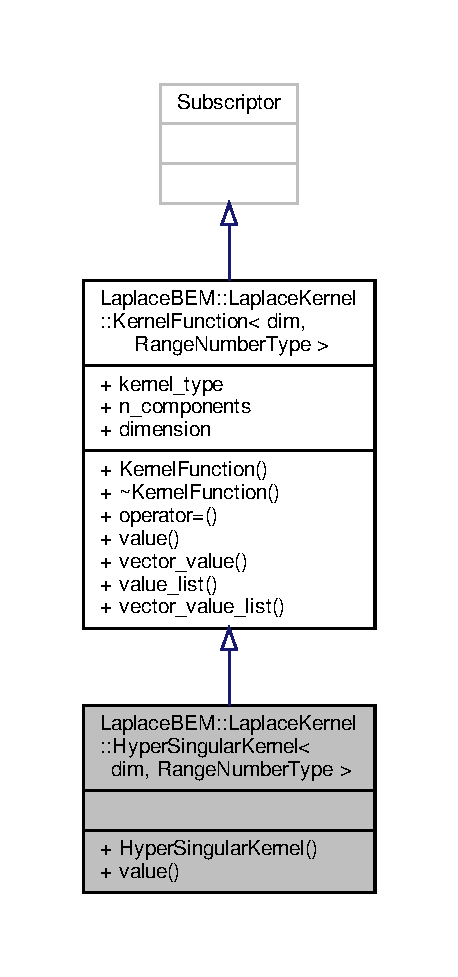
\includegraphics[width=220pt]{classLaplaceBEM_1_1LaplaceKernel_1_1HyperSingularKernel__inherit__graph}
\end{center}
\end{figure}


Collaboration diagram for Laplace\+B\+EM\+:\+:Laplace\+Kernel\+:\+:Hyper\+Singular\+Kernel$<$ dim, Range\+Number\+Type $>$\+:\nopagebreak
\begin{figure}[H]
\begin{center}
\leavevmode
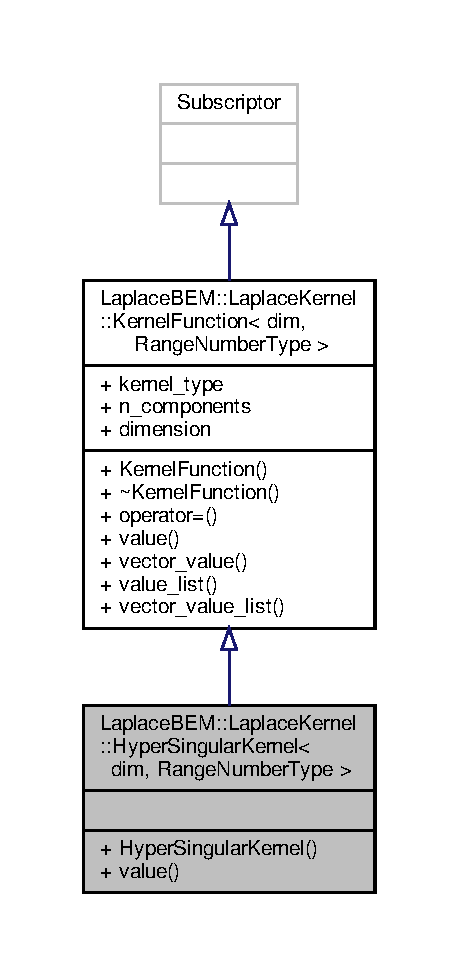
\includegraphics[width=220pt]{classLaplaceBEM_1_1LaplaceKernel_1_1HyperSingularKernel__coll__graph}
\end{center}
\end{figure}
\subsection*{Public Member Functions}
\begin{DoxyCompactItemize}
\item 
virtual Range\+Number\+Type \hyperlink{classLaplaceBEM_1_1LaplaceKernel_1_1HyperSingularKernel_a02811fc623d2bb605c5eeb22712bdfd6}{value} (const Point$<$ dim $>$ \&x, const Point$<$ dim $>$ \&y, const Tensor$<$ 1, dim $>$ \&nx, const Tensor$<$ 1, dim $>$ \&ny, const unsigned int component=0) const override
\end{DoxyCompactItemize}
\subsection*{Additional Inherited Members}


\subsection{Member Function Documentation}
\mbox{\Hypertarget{classLaplaceBEM_1_1LaplaceKernel_1_1HyperSingularKernel_a02811fc623d2bb605c5eeb22712bdfd6}\label{classLaplaceBEM_1_1LaplaceKernel_1_1HyperSingularKernel_a02811fc623d2bb605c5eeb22712bdfd6}} 
\index{Laplace\+B\+E\+M\+::\+Laplace\+Kernel\+::\+Hyper\+Singular\+Kernel@{Laplace\+B\+E\+M\+::\+Laplace\+Kernel\+::\+Hyper\+Singular\+Kernel}!value@{value}}
\index{value@{value}!Laplace\+B\+E\+M\+::\+Laplace\+Kernel\+::\+Hyper\+Singular\+Kernel@{Laplace\+B\+E\+M\+::\+Laplace\+Kernel\+::\+Hyper\+Singular\+Kernel}}
\subsubsection{\texorpdfstring{value()}{value()}}
{\footnotesize\ttfamily template$<$int dim, typename Range\+Number\+Type $>$ \\
Range\+Number\+Type \hyperlink{classLaplaceBEM_1_1LaplaceKernel_1_1HyperSingularKernel}{Laplace\+B\+E\+M\+::\+Laplace\+Kernel\+::\+Hyper\+Singular\+Kernel}$<$ dim, Range\+Number\+Type $>$\+::value (\begin{DoxyParamCaption}\item[{const Point$<$ dim $>$ \&}]{x,  }\item[{const Point$<$ dim $>$ \&}]{y,  }\item[{const Tensor$<$ 1, dim $>$ \&}]{nx,  }\item[{const Tensor$<$ 1, dim $>$ \&}]{ny,  }\item[{const unsigned int}]{component = {\ttfamily 0} }\end{DoxyParamCaption}) const\hspace{0.3cm}{\ttfamily [override]}, {\ttfamily [virtual]}}

Evaluate the kernel function at the specified point pair $(x, y)$ associated with their normal vectors $(n_x, n_y)$. In case the kernel function is vector-\/valued, this function only returns the required {\ttfamily component} in the result vector.


\begin{DoxyParams}{Parameters}
{\em x} & \\
\hline
{\em y} & \\
\hline
{\em nx} & \\
\hline
{\em ny} & \\
\hline
{\em component} & Component index in the result vector, if the kernel function is vector-\/valued. If the kernel function is scalar-\/valued, there is no such issue and {\ttfamily component} is 0 by default. \\
\hline
\end{DoxyParams}
\begin{DoxyReturn}{Returns}

\end{DoxyReturn}
This function should never be called, since as a member function of the abstract class, it has no literal definition of the function. Hence, we throw an error here.

Reimplemented from \hyperlink{classLaplaceBEM_1_1LaplaceKernel_1_1KernelFunction_aee6c638a4392616e89784d7b6558dd24}{Laplace\+B\+E\+M\+::\+Laplace\+Kernel\+::\+Kernel\+Function$<$ dim, Range\+Number\+Type $>$}.



The documentation for this class was generated from the following file\+:\begin{DoxyCompactItemize}
\item 
/home/jihuan/\+Projects/deal.\+ii/program/dealii-\/9.\+1.\+1/examples/laplace-\/bem/include/\hyperlink{laplace__bem_8h}{laplace\+\_\+bem.\+h}\end{DoxyCompactItemize}

\hypertarget{classLaplaceBEM_1_1LaplaceKernel_1_1KernelFunction}{}\section{Laplace\+B\+EM\+:\+:Laplace\+Kernel\+:\+:Kernel\+Function$<$ dim, Range\+Number\+Type $>$ Class Template Reference}
\label{classLaplaceBEM_1_1LaplaceKernel_1_1KernelFunction}\index{Laplace\+B\+E\+M\+::\+Laplace\+Kernel\+::\+Kernel\+Function$<$ dim, Range\+Number\+Type $>$@{Laplace\+B\+E\+M\+::\+Laplace\+Kernel\+::\+Kernel\+Function$<$ dim, Range\+Number\+Type $>$}}


{\ttfamily \#include $<$laplace\+\_\+bem.\+h$>$}



Inheritance diagram for Laplace\+B\+EM\+:\+:Laplace\+Kernel\+:\+:Kernel\+Function$<$ dim, Range\+Number\+Type $>$\+:\nopagebreak
\begin{figure}[H]
\begin{center}
\leavevmode
\includegraphics[width=350pt]{classLaplaceBEM_1_1LaplaceKernel_1_1KernelFunction__inherit__graph}
\end{center}
\end{figure}


Collaboration diagram for Laplace\+B\+EM\+:\+:Laplace\+Kernel\+:\+:Kernel\+Function$<$ dim, Range\+Number\+Type $>$\+:\nopagebreak
\begin{figure}[H]
\begin{center}
\leavevmode
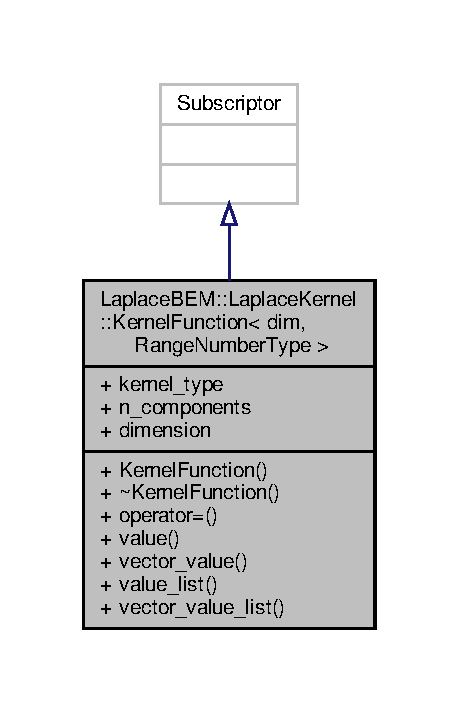
\includegraphics[width=220pt]{classLaplaceBEM_1_1LaplaceKernel_1_1KernelFunction__coll__graph}
\end{center}
\end{figure}
\subsection*{Public Member Functions}
\begin{DoxyCompactItemize}
\item 
\mbox{\Hypertarget{classLaplaceBEM_1_1LaplaceKernel_1_1KernelFunction_a1f10a1886e4b9aed7d60c036ccc81ee6}\label{classLaplaceBEM_1_1LaplaceKernel_1_1KernelFunction_a1f10a1886e4b9aed7d60c036ccc81ee6}} 
{\bfseries Kernel\+Function} (const Kernel\+Type kernel\+\_\+type=None\+Type, const unsigned int n\+\_\+components=1)
\item 
virtual \hyperlink{classLaplaceBEM_1_1LaplaceKernel_1_1KernelFunction_a2611849d182d0869c6f07026416305b3}{$\sim$\+Kernel\+Function} () override=0
\item 
\hyperlink{classLaplaceBEM_1_1LaplaceKernel_1_1KernelFunction}{Kernel\+Function} \& \hyperlink{classLaplaceBEM_1_1LaplaceKernel_1_1KernelFunction_a2a9a7e11aca4e52ece2d721e60a4bf56}{operator=} (const \hyperlink{classLaplaceBEM_1_1LaplaceKernel_1_1KernelFunction}{Kernel\+Function} \&f)
\item 
virtual Range\+Number\+Type \hyperlink{classLaplaceBEM_1_1LaplaceKernel_1_1KernelFunction_aee6c638a4392616e89784d7b6558dd24}{value} (const Point$<$ dim $>$ \&x, const Point$<$ dim $>$ \&y, const Tensor$<$ 1, dim $>$ \&nx, const Tensor$<$ 1, dim $>$ \&ny, const unsigned int component=0) const
\item 
virtual void \hyperlink{classLaplaceBEM_1_1LaplaceKernel_1_1KernelFunction_aa8110379ffcda0d7aabeb1b9229fa8db}{vector\+\_\+value} (const Point$<$ dim $>$ \&x, const Point$<$ dim $>$ \&y, const Tensor$<$ 1, dim $>$ \&nx, const Tensor$<$ 1, dim $>$ \&ny, Vector$<$ Range\+Number\+Type $>$ \&values) const
\item 
virtual void \hyperlink{classLaplaceBEM_1_1LaplaceKernel_1_1KernelFunction_a8ba5755bf65478154209736c001f2f2a}{value\+\_\+list} (const std\+::vector$<$ Point$<$ dim $>$$>$ \&x\+\_\+points, const std\+::vector$<$ Point$<$ dim $>$$>$ \&y\+\_\+points, const std\+::vector$<$ Tensor$<$ 1, dim $>$$>$ \&nx\+\_\+list, const std\+::vector$<$ Tensor$<$ 1, dim $>$$>$ \&ny\+\_\+list, std\+::vector$<$ Range\+Number\+Type $>$ \&values, const unsigned int component=0) const
\item 
virtual void \hyperlink{classLaplaceBEM_1_1LaplaceKernel_1_1KernelFunction_ae906434f76ac27668ab4ddf91e3cd7fb}{vector\+\_\+value\+\_\+list} (const std\+::vector$<$ Point$<$ dim $>$$>$ \&x\+\_\+points, const std\+::vector$<$ Point$<$ dim $>$$>$ \&y\+\_\+points, const std\+::vector$<$ Tensor$<$ 1, dim $>$$>$ \&nx\+\_\+list, const std\+::vector$<$ Tensor$<$ 1, dim $>$$>$ \&ny\+\_\+list, std\+::vector$<$ Vector$<$ Range\+Number\+Type $>$$>$ \&values) const
\end{DoxyCompactItemize}
\subsection*{Public Attributes}
\begin{DoxyCompactItemize}
\item 
\mbox{\Hypertarget{classLaplaceBEM_1_1LaplaceKernel_1_1KernelFunction_a4e4f538fccd38abfa5619c10cedeae00}\label{classLaplaceBEM_1_1LaplaceKernel_1_1KernelFunction_a4e4f538fccd38abfa5619c10cedeae00}} 
const Kernel\+Type {\bfseries kernel\+\_\+type}
\item 
\mbox{\Hypertarget{classLaplaceBEM_1_1LaplaceKernel_1_1KernelFunction_a21908b76243d0b7b3b61ef67871ed790}\label{classLaplaceBEM_1_1LaplaceKernel_1_1KernelFunction_a21908b76243d0b7b3b61ef67871ed790}} 
const unsigned int {\bfseries n\+\_\+components}
\end{DoxyCompactItemize}
\subsection*{Static Public Attributes}
\begin{DoxyCompactItemize}
\item 
\mbox{\Hypertarget{classLaplaceBEM_1_1LaplaceKernel_1_1KernelFunction_ad4cf29ad18c345f5d6d781a1b4aad15a}\label{classLaplaceBEM_1_1LaplaceKernel_1_1KernelFunction_ad4cf29ad18c345f5d6d781a1b4aad15a}} 
static const unsigned int {\bfseries dimension} = dim
\end{DoxyCompactItemize}


\subsection{Detailed Description}
\subsubsection*{template$<$int dim, typename Range\+Number\+Type = double$>$\newline
class Laplace\+B\+E\+M\+::\+Laplace\+Kernel\+::\+Kernel\+Function$<$ dim, Range\+Number\+Type $>$}

Base class for a B\+EM Laplace kernel function.


\begin{DoxyDescription}
\item[Note ]The template argument {\ttfamily dim} is the spatial dimension instead of the manifold dimension. 
\end{DoxyDescription}

\subsection{Constructor \& Destructor Documentation}
\mbox{\Hypertarget{classLaplaceBEM_1_1LaplaceKernel_1_1KernelFunction_a2611849d182d0869c6f07026416305b3}\label{classLaplaceBEM_1_1LaplaceKernel_1_1KernelFunction_a2611849d182d0869c6f07026416305b3}} 
\index{Laplace\+B\+E\+M\+::\+Laplace\+Kernel\+::\+Kernel\+Function@{Laplace\+B\+E\+M\+::\+Laplace\+Kernel\+::\+Kernel\+Function}!````~Kernel\+Function@{$\sim$\+Kernel\+Function}}
\index{````~Kernel\+Function@{$\sim$\+Kernel\+Function}!Laplace\+B\+E\+M\+::\+Laplace\+Kernel\+::\+Kernel\+Function@{Laplace\+B\+E\+M\+::\+Laplace\+Kernel\+::\+Kernel\+Function}}
\subsubsection{\texorpdfstring{$\sim$\+Kernel\+Function()}{~KernelFunction()}}
{\footnotesize\ttfamily template$<$int dim, typename Range\+Number\+Type $>$ \\
\hyperlink{classLaplaceBEM_1_1LaplaceKernel_1_1KernelFunction}{Laplace\+B\+E\+M\+::\+Laplace\+Kernel\+::\+Kernel\+Function}$<$ dim, Range\+Number\+Type $>$\+::$\sim$\hyperlink{classLaplaceBEM_1_1LaplaceKernel_1_1KernelFunction}{Kernel\+Function} (\begin{DoxyParamCaption}{ }\end{DoxyParamCaption})\hspace{0.3cm}{\ttfamily [inline]}, {\ttfamily [override]}, {\ttfamily [pure virtual]}, {\ttfamily [default]}}

Default destructor provided by the compiler. 

\subsection{Member Function Documentation}
\mbox{\Hypertarget{classLaplaceBEM_1_1LaplaceKernel_1_1KernelFunction_a2a9a7e11aca4e52ece2d721e60a4bf56}\label{classLaplaceBEM_1_1LaplaceKernel_1_1KernelFunction_a2a9a7e11aca4e52ece2d721e60a4bf56}} 
\index{Laplace\+B\+E\+M\+::\+Laplace\+Kernel\+::\+Kernel\+Function@{Laplace\+B\+E\+M\+::\+Laplace\+Kernel\+::\+Kernel\+Function}!operator=@{operator=}}
\index{operator=@{operator=}!Laplace\+B\+E\+M\+::\+Laplace\+Kernel\+::\+Kernel\+Function@{Laplace\+B\+E\+M\+::\+Laplace\+Kernel\+::\+Kernel\+Function}}
\subsubsection{\texorpdfstring{operator=()}{operator=()}}
{\footnotesize\ttfamily template$<$int dim, typename Range\+Number\+Type $>$ \\
\hyperlink{classLaplaceBEM_1_1LaplaceKernel_1_1KernelFunction}{Kernel\+Function}$<$ dim, Range\+Number\+Type $>$ \& \hyperlink{classLaplaceBEM_1_1LaplaceKernel_1_1KernelFunction}{Laplace\+B\+E\+M\+::\+Laplace\+Kernel\+::\+Kernel\+Function}$<$ dim, Range\+Number\+Type $>$\+::operator= (\begin{DoxyParamCaption}\item[{const \hyperlink{classLaplaceBEM_1_1LaplaceKernel_1_1KernelFunction}{Kernel\+Function}$<$ dim, Range\+Number\+Type $>$ \&}]{f }\end{DoxyParamCaption})}

Assignment operator


\begin{DoxyParams}{Parameters}
{\em f} & \\
\hline
\end{DoxyParams}
\begin{DoxyReturn}{Returns}

\end{DoxyReturn}
As a pure base class, it does nothing here but only assert the number of components. The following sentence suppresses compiler warnings about the unused input argument f.\mbox{\Hypertarget{classLaplaceBEM_1_1LaplaceKernel_1_1KernelFunction_aee6c638a4392616e89784d7b6558dd24}\label{classLaplaceBEM_1_1LaplaceKernel_1_1KernelFunction_aee6c638a4392616e89784d7b6558dd24}} 
\index{Laplace\+B\+E\+M\+::\+Laplace\+Kernel\+::\+Kernel\+Function@{Laplace\+B\+E\+M\+::\+Laplace\+Kernel\+::\+Kernel\+Function}!value@{value}}
\index{value@{value}!Laplace\+B\+E\+M\+::\+Laplace\+Kernel\+::\+Kernel\+Function@{Laplace\+B\+E\+M\+::\+Laplace\+Kernel\+::\+Kernel\+Function}}
\subsubsection{\texorpdfstring{value()}{value()}}
{\footnotesize\ttfamily template$<$int dim, typename Range\+Number\+Type $>$ \\
Range\+Number\+Type \hyperlink{classLaplaceBEM_1_1LaplaceKernel_1_1KernelFunction}{Laplace\+B\+E\+M\+::\+Laplace\+Kernel\+::\+Kernel\+Function}$<$ dim, Range\+Number\+Type $>$\+::value (\begin{DoxyParamCaption}\item[{const Point$<$ dim $>$ \&}]{x,  }\item[{const Point$<$ dim $>$ \&}]{y,  }\item[{const Tensor$<$ 1, dim $>$ \&}]{nx,  }\item[{const Tensor$<$ 1, dim $>$ \&}]{ny,  }\item[{const unsigned int}]{component = {\ttfamily 0} }\end{DoxyParamCaption}) const\hspace{0.3cm}{\ttfamily [virtual]}}

Evaluate the kernel function at the specified point pair $(x, y)$ associated with their normal vectors $(n_x, n_y)$. In case the kernel function is vector-\/valued, this function only returns the required {\ttfamily component} in the result vector.


\begin{DoxyParams}{Parameters}
{\em x} & \\
\hline
{\em y} & \\
\hline
{\em nx} & \\
\hline
{\em ny} & \\
\hline
{\em component} & Component index in the result vector, if the kernel function is vector-\/valued. If the kernel function is scalar-\/valued, there is no such issue and {\ttfamily component} is 0 by default. \\
\hline
\end{DoxyParams}
\begin{DoxyReturn}{Returns}

\end{DoxyReturn}
This function should never be called, since as a member function of the abstract class, it has no literal definition of the function. Hence, we throw an error here.

Reimplemented in \hyperlink{classLaplaceBEM_1_1LaplaceKernel_1_1HyperSingularKernel_a02811fc623d2bb605c5eeb22712bdfd6}{Laplace\+B\+E\+M\+::\+Laplace\+Kernel\+::\+Hyper\+Singular\+Kernel$<$ dim, Range\+Number\+Type $>$}, \hyperlink{classLaplaceBEM_1_1LaplaceKernel_1_1AdjointDoubleLayerKernel_acfa06279ea767680f2fbefee07a34304}{Laplace\+B\+E\+M\+::\+Laplace\+Kernel\+::\+Adjoint\+Double\+Layer\+Kernel$<$ dim, Range\+Number\+Type $>$}, \hyperlink{classLaplaceBEM_1_1LaplaceKernel_1_1DoubleLayerKernel_a44836d10e150f631a40d16dc2092fdad}{Laplace\+B\+E\+M\+::\+Laplace\+Kernel\+::\+Double\+Layer\+Kernel$<$ dim, Range\+Number\+Type $>$}, \hyperlink{classLaplaceBEM_1_1LaplaceKernel_1_1DoubleLayerKernel_a44836d10e150f631a40d16dc2092fdad}{Laplace\+B\+E\+M\+::\+Laplace\+Kernel\+::\+Double\+Layer\+Kernel$<$ 3 $>$}, \hyperlink{classLaplaceBEM_1_1LaplaceKernel_1_1SingleLayerKernel_a657e04bd67d8c33adeea1b9d282d6136}{Laplace\+B\+E\+M\+::\+Laplace\+Kernel\+::\+Single\+Layer\+Kernel$<$ dim, Range\+Number\+Type $>$}, and \hyperlink{classLaplaceBEM_1_1LaplaceKernel_1_1SingleLayerKernel_a657e04bd67d8c33adeea1b9d282d6136}{Laplace\+B\+E\+M\+::\+Laplace\+Kernel\+::\+Single\+Layer\+Kernel$<$ 3 $>$}.

\mbox{\Hypertarget{classLaplaceBEM_1_1LaplaceKernel_1_1KernelFunction_a8ba5755bf65478154209736c001f2f2a}\label{classLaplaceBEM_1_1LaplaceKernel_1_1KernelFunction_a8ba5755bf65478154209736c001f2f2a}} 
\index{Laplace\+B\+E\+M\+::\+Laplace\+Kernel\+::\+Kernel\+Function@{Laplace\+B\+E\+M\+::\+Laplace\+Kernel\+::\+Kernel\+Function}!value\+\_\+list@{value\+\_\+list}}
\index{value\+\_\+list@{value\+\_\+list}!Laplace\+B\+E\+M\+::\+Laplace\+Kernel\+::\+Kernel\+Function@{Laplace\+B\+E\+M\+::\+Laplace\+Kernel\+::\+Kernel\+Function}}
\subsubsection{\texorpdfstring{value\+\_\+list()}{value\_list()}}
{\footnotesize\ttfamily template$<$int dim, typename Range\+Number\+Type$>$ \\
void \hyperlink{classLaplaceBEM_1_1LaplaceKernel_1_1KernelFunction}{Laplace\+B\+E\+M\+::\+Laplace\+Kernel\+::\+Kernel\+Function}$<$ dim, Range\+Number\+Type $>$\+::value\+\_\+list (\begin{DoxyParamCaption}\item[{const std\+::vector$<$ Point$<$ dim $>$$>$ \&}]{x\+\_\+points,  }\item[{const std\+::vector$<$ Point$<$ dim $>$$>$ \&}]{y\+\_\+points,  }\item[{const std\+::vector$<$ Tensor$<$ 1, dim $>$$>$ \&}]{nx\+\_\+list,  }\item[{const std\+::vector$<$ Tensor$<$ 1, dim $>$$>$ \&}]{ny\+\_\+list,  }\item[{std\+::vector$<$ Range\+Number\+Type $>$ \&}]{values,  }\item[{const unsigned int}]{component = {\ttfamily 0} }\end{DoxyParamCaption}) const\hspace{0.3cm}{\ttfamily [virtual]}}

Define the default behavior for evaluation of {\ttfamily \hyperlink{classLaplaceBEM_1_1LaplaceKernel_1_1KernelFunction_aee6c638a4392616e89784d7b6558dd24}{Kernel\+Function\+::value}} at a list of points with associated normal vectors $(n_x, n_y)$. Only the required {\ttfamily component} in the result vector will be returned, if the kernel function is vector-\/valued.


\begin{DoxyDescription}
\item[Note ]Even though {\ttfamily \hyperlink{classLaplaceBEM_1_1LaplaceKernel_1_1KernelFunction}{Kernel\+Function}} is an abstract class which cannot be instantiated and its member functions will never be called, the definition of this function will reduce the burden of redefining such function in each child class. 
\end{DoxyDescription}


\begin{DoxyParams}{Parameters}
{\em x\+\_\+points} & \\
\hline
{\em y\+\_\+points} & \\
\hline
{\em nx\+\_\+list} & \\
\hline
{\em ny\+\_\+list} & \\
\hline
{\em values} & \\
\hline
{\em component} & \\
\hline
\end{DoxyParams}
\mbox{\Hypertarget{classLaplaceBEM_1_1LaplaceKernel_1_1KernelFunction_aa8110379ffcda0d7aabeb1b9229fa8db}\label{classLaplaceBEM_1_1LaplaceKernel_1_1KernelFunction_aa8110379ffcda0d7aabeb1b9229fa8db}} 
\index{Laplace\+B\+E\+M\+::\+Laplace\+Kernel\+::\+Kernel\+Function@{Laplace\+B\+E\+M\+::\+Laplace\+Kernel\+::\+Kernel\+Function}!vector\+\_\+value@{vector\+\_\+value}}
\index{vector\+\_\+value@{vector\+\_\+value}!Laplace\+B\+E\+M\+::\+Laplace\+Kernel\+::\+Kernel\+Function@{Laplace\+B\+E\+M\+::\+Laplace\+Kernel\+::\+Kernel\+Function}}
\subsubsection{\texorpdfstring{vector\+\_\+value()}{vector\_value()}}
{\footnotesize\ttfamily template$<$int dim, typename Range\+Number\+Type$>$ \\
void \hyperlink{classLaplaceBEM_1_1LaplaceKernel_1_1KernelFunction}{Laplace\+B\+E\+M\+::\+Laplace\+Kernel\+::\+Kernel\+Function}$<$ dim, Range\+Number\+Type $>$\+::vector\+\_\+value (\begin{DoxyParamCaption}\item[{const Point$<$ dim $>$ \&}]{x,  }\item[{const Point$<$ dim $>$ \&}]{y,  }\item[{const Tensor$<$ 1, dim $>$ \&}]{nx,  }\item[{const Tensor$<$ 1, dim $>$ \&}]{ny,  }\item[{Vector$<$ Range\+Number\+Type $>$ \&}]{values }\end{DoxyParamCaption}) const\hspace{0.3cm}{\ttfamily [virtual]}}

Define the default behavior for evaluation of {\ttfamily \hyperlink{classLaplaceBEM_1_1LaplaceKernel_1_1KernelFunction_aee6c638a4392616e89784d7b6558dd24}{Kernel\+Function\+::value}} at the specified point pair $(x, y)$ associated with their normal vectors $(n_x, n_y)$ and all of its components will be retrieved into the result vector {\ttfamily values}.


\begin{DoxyDescription}
\item[Note ]Even though {\ttfamily \hyperlink{classLaplaceBEM_1_1LaplaceKernel_1_1KernelFunction}{Kernel\+Function}} is an abstract class which cannot be instantiated and its member functions will never be called, the definition of this function will reduce the burden of redefining such function in each child class. 
\end{DoxyDescription}


\begin{DoxyParams}{Parameters}
{\em x} & \\
\hline
{\em y} & \\
\hline
{\em nx} & \\
\hline
{\em ny} & \\
\hline
{\em values} & The vector holding all components of the function result. \\
\hline
\end{DoxyParams}
\mbox{\Hypertarget{classLaplaceBEM_1_1LaplaceKernel_1_1KernelFunction_ae906434f76ac27668ab4ddf91e3cd7fb}\label{classLaplaceBEM_1_1LaplaceKernel_1_1KernelFunction_ae906434f76ac27668ab4ddf91e3cd7fb}} 
\index{Laplace\+B\+E\+M\+::\+Laplace\+Kernel\+::\+Kernel\+Function@{Laplace\+B\+E\+M\+::\+Laplace\+Kernel\+::\+Kernel\+Function}!vector\+\_\+value\+\_\+list@{vector\+\_\+value\+\_\+list}}
\index{vector\+\_\+value\+\_\+list@{vector\+\_\+value\+\_\+list}!Laplace\+B\+E\+M\+::\+Laplace\+Kernel\+::\+Kernel\+Function@{Laplace\+B\+E\+M\+::\+Laplace\+Kernel\+::\+Kernel\+Function}}
\subsubsection{\texorpdfstring{vector\+\_\+value\+\_\+list()}{vector\_value\_list()}}
{\footnotesize\ttfamily template$<$int dim, typename Range\+Number\+Type$>$ \\
void \hyperlink{classLaplaceBEM_1_1LaplaceKernel_1_1KernelFunction}{Laplace\+B\+E\+M\+::\+Laplace\+Kernel\+::\+Kernel\+Function}$<$ dim, Range\+Number\+Type $>$\+::vector\+\_\+value\+\_\+list (\begin{DoxyParamCaption}\item[{const std\+::vector$<$ Point$<$ dim $>$$>$ \&}]{x\+\_\+points,  }\item[{const std\+::vector$<$ Point$<$ dim $>$$>$ \&}]{y\+\_\+points,  }\item[{const std\+::vector$<$ Tensor$<$ 1, dim $>$$>$ \&}]{nx\+\_\+list,  }\item[{const std\+::vector$<$ Tensor$<$ 1, dim $>$$>$ \&}]{ny\+\_\+list,  }\item[{std\+::vector$<$ Vector$<$ Range\+Number\+Type $>$$>$ \&}]{values }\end{DoxyParamCaption}) const\hspace{0.3cm}{\ttfamily [virtual]}}

Define the default behavior for evaluation of {\ttfamily \hyperlink{classLaplaceBEM_1_1LaplaceKernel_1_1KernelFunction_aa8110379ffcda0d7aabeb1b9229fa8db}{Kernel\+Function\+::vector\+\_\+value}} at a list of points with associated normal vectors $(n_x, n_y)$.


\begin{DoxyDescription}
\item[Note ]Even though {\ttfamily \hyperlink{classLaplaceBEM_1_1LaplaceKernel_1_1KernelFunction}{Kernel\+Function}} is an abstract class which cannot be instantiated and its member functions will never be called, the definition of this function will reduce the burden of redefining such function in each child class. 
\end{DoxyDescription}


\begin{DoxyParams}{Parameters}
{\em x\+\_\+points} & \\
\hline
{\em y\+\_\+points} & \\
\hline
{\em nx\+\_\+list} & \\
\hline
{\em ny\+\_\+list} & \\
\hline
{\em values} & \\
\hline
\end{DoxyParams}


The documentation for this class was generated from the following file\+:\begin{DoxyCompactItemize}
\item 
/home/jihuan/\+Projects/deal.\+ii/program/dealii-\/9.\+1.\+1/examples/laplace-\/bem/include/\hyperlink{laplace__bem_8h}{laplace\+\_\+bem.\+h}\end{DoxyCompactItemize}

\hypertarget{classLaplaceBEM_1_1KernelPulledbackToSauterSpace}{}\section{Laplace\+B\+EM\+:\+:Kernel\+Pulledback\+To\+Sauter\+Space$<$ dim, spacedim, Range\+Number\+Type $>$ Class Template Reference}
\label{classLaplaceBEM_1_1KernelPulledbackToSauterSpace}\index{Laplace\+B\+E\+M\+::\+Kernel\+Pulledback\+To\+Sauter\+Space$<$ dim, spacedim, Range\+Number\+Type $>$@{Laplace\+B\+E\+M\+::\+Kernel\+Pulledback\+To\+Sauter\+Space$<$ dim, spacedim, Range\+Number\+Type $>$}}


{\ttfamily \#include $<$laplace\+\_\+bem.\+h$>$}



Inheritance diagram for Laplace\+B\+EM\+:\+:Kernel\+Pulledback\+To\+Sauter\+Space$<$ dim, spacedim, Range\+Number\+Type $>$\+:\nopagebreak
\begin{figure}[H]
\begin{center}
\leavevmode
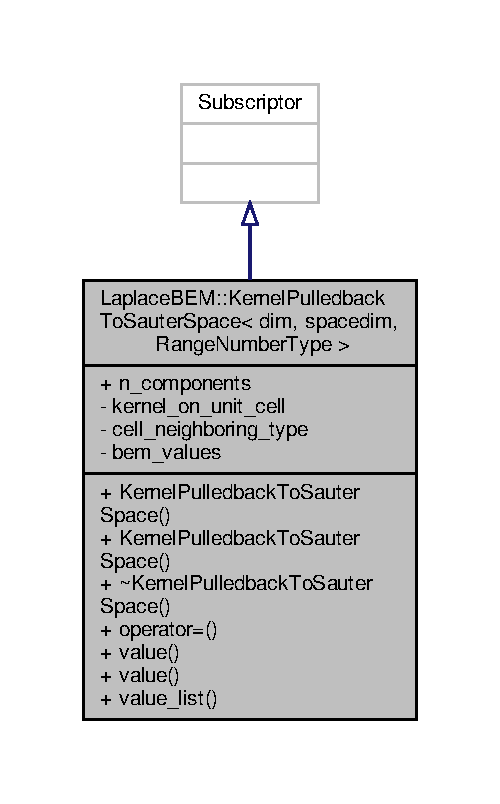
\includegraphics[width=240pt]{classLaplaceBEM_1_1KernelPulledbackToSauterSpace__inherit__graph}
\end{center}
\end{figure}


Collaboration diagram for Laplace\+B\+EM\+:\+:Kernel\+Pulledback\+To\+Sauter\+Space$<$ dim, spacedim, Range\+Number\+Type $>$\+:\nopagebreak
\begin{figure}[H]
\begin{center}
\leavevmode
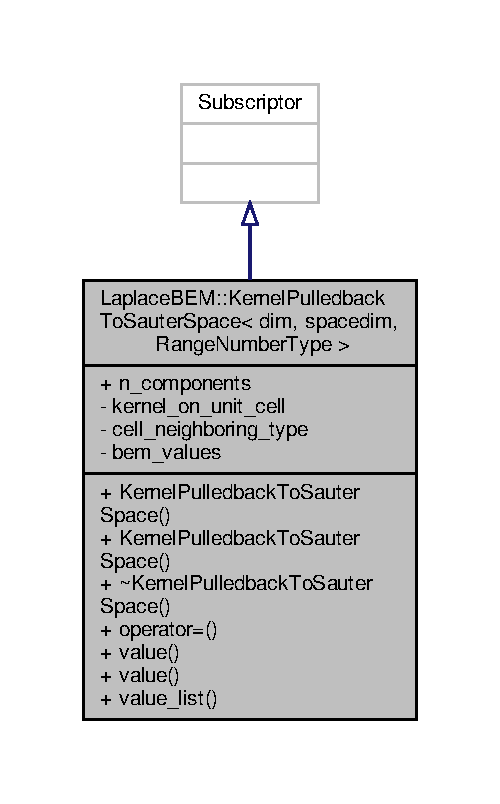
\includegraphics[width=240pt]{classLaplaceBEM_1_1KernelPulledbackToSauterSpace__coll__graph}
\end{center}
\end{figure}
\subsection*{Public Member Functions}
\begin{DoxyCompactItemize}
\item 
\mbox{\Hypertarget{classLaplaceBEM_1_1KernelPulledbackToSauterSpace_a84d8a1b230bab697000f16e021c671a4}\label{classLaplaceBEM_1_1KernelPulledbackToSauterSpace_a84d8a1b230bab697000f16e021c671a4}} 
{\bfseries Kernel\+Pulledback\+To\+Sauter\+Space} (const \hyperlink{classLaplaceBEM_1_1KernelPulledbackToUnitCell}{Kernel\+Pulledback\+To\+Unit\+Cell}$<$ dim, spacedim, Range\+Number\+Type $>$ \&kernel, const Cell\+Neighboring\+Type cell\+\_\+neighboring\+\_\+type)
\item 
\mbox{\Hypertarget{classLaplaceBEM_1_1KernelPulledbackToSauterSpace_ae5d75fcb617d831107a8cd2151e6cb3a}\label{classLaplaceBEM_1_1KernelPulledbackToSauterSpace_ae5d75fcb617d831107a8cd2151e6cb3a}} 
{\bfseries Kernel\+Pulledback\+To\+Sauter\+Space} (const \hyperlink{classLaplaceBEM_1_1KernelPulledbackToUnitCell}{Kernel\+Pulledback\+To\+Unit\+Cell}$<$ dim, spacedim, Range\+Number\+Type $>$ \&kernel, const Cell\+Neighboring\+Type cell\+\_\+neighboring\+\_\+type, const \hyperlink{classLaplaceBEM_1_1BEMValues}{B\+E\+M\+Values}$<$ dim, spacedim, Range\+Number\+Type $>$ $\ast$bem\+\_\+values)
\item 
\mbox{\Hypertarget{classLaplaceBEM_1_1KernelPulledbackToSauterSpace_a6c0754fea80b064e1b8b7246634d0cb9}\label{classLaplaceBEM_1_1KernelPulledbackToSauterSpace_a6c0754fea80b064e1b8b7246634d0cb9}} 
\hyperlink{classLaplaceBEM_1_1KernelPulledbackToSauterSpace}{Kernel\+Pulledback\+To\+Sauter\+Space} \& {\bfseries operator=} (const \hyperlink{classLaplaceBEM_1_1KernelPulledbackToSauterSpace}{Kernel\+Pulledback\+To\+Sauter\+Space} \&f)
\item 
Range\+Number\+Type \hyperlink{classLaplaceBEM_1_1KernelPulledbackToSauterSpace_a27d5e8b248c5060198b9137162d77c0c}{value} (const Point$<$ dim $\ast$2 $>$ p, const unsigned int component=0) const
\item 
Range\+Number\+Type \hyperlink{classLaplaceBEM_1_1KernelPulledbackToSauterSpace_a3f811601a201e4c68cd1a9392866706b}{value} (const unsigned int quad\+\_\+no, const unsigned int component=0) const
\item 
\mbox{\Hypertarget{classLaplaceBEM_1_1KernelPulledbackToSauterSpace_aed5c1c302117781dd5c0460cfc8a9392}\label{classLaplaceBEM_1_1KernelPulledbackToSauterSpace_aed5c1c302117781dd5c0460cfc8a9392}} 
void {\bfseries value\+\_\+list} (const std\+::vector$<$ Point$<$ dim $\ast$2 $>$$>$ \&points, std\+::vector$<$ Range\+Number\+Type $>$ \&values, const unsigned int component=0) const
\end{DoxyCompactItemize}
\subsection*{Public Attributes}
\begin{DoxyCompactItemize}
\item 
\mbox{\Hypertarget{classLaplaceBEM_1_1KernelPulledbackToSauterSpace_a8e401c7c6e032c8cd25f45f404179319}\label{classLaplaceBEM_1_1KernelPulledbackToSauterSpace_a8e401c7c6e032c8cd25f45f404179319}} 
const unsigned int {\bfseries n\+\_\+components}
\end{DoxyCompactItemize}
\subsection*{Private Attributes}
\begin{DoxyCompactItemize}
\item 
\mbox{\Hypertarget{classLaplaceBEM_1_1KernelPulledbackToSauterSpace_af9313eea69535eb0e01ead937e9028c0}\label{classLaplaceBEM_1_1KernelPulledbackToSauterSpace_af9313eea69535eb0e01ead937e9028c0}} 
const \hyperlink{classLaplaceBEM_1_1KernelPulledbackToUnitCell}{Kernel\+Pulledback\+To\+Unit\+Cell}$<$ dim, spacedim, Range\+Number\+Type $>$ \& {\bfseries kernel\+\_\+on\+\_\+unit\+\_\+cell}
\item 
\mbox{\Hypertarget{classLaplaceBEM_1_1KernelPulledbackToSauterSpace_aa9e897f0e63f3c7ee5009c07e66cbd56}\label{classLaplaceBEM_1_1KernelPulledbackToSauterSpace_aa9e897f0e63f3c7ee5009c07e66cbd56}} 
Cell\+Neighboring\+Type {\bfseries cell\+\_\+neighboring\+\_\+type}
\item 
\mbox{\Hypertarget{classLaplaceBEM_1_1KernelPulledbackToSauterSpace_a5bcaf6a268588034723b37b4bd858476}\label{classLaplaceBEM_1_1KernelPulledbackToSauterSpace_a5bcaf6a268588034723b37b4bd858476}} 
const \hyperlink{classLaplaceBEM_1_1BEMValues}{B\+E\+M\+Values}$<$ dim, spacedim, Range\+Number\+Type $>$ $\ast$ {\bfseries bem\+\_\+values}
\end{DoxyCompactItemize}


\subsection{Detailed Description}
\subsubsection*{template$<$int dim, int spacedim, typename Range\+Number\+Type = double$>$\newline
class Laplace\+B\+E\+M\+::\+Kernel\+Pulledback\+To\+Sauter\+Space$<$ dim, spacedim, Range\+Number\+Type $>$}

Class for pullback the kernel function on the product of two unit cells to Sauter\textquotesingle{}s parametric space. 

\subsection{Member Function Documentation}
\mbox{\Hypertarget{classLaplaceBEM_1_1KernelPulledbackToSauterSpace_a27d5e8b248c5060198b9137162d77c0c}\label{classLaplaceBEM_1_1KernelPulledbackToSauterSpace_a27d5e8b248c5060198b9137162d77c0c}} 
\index{Laplace\+B\+E\+M\+::\+Kernel\+Pulledback\+To\+Sauter\+Space@{Laplace\+B\+E\+M\+::\+Kernel\+Pulledback\+To\+Sauter\+Space}!value@{value}}
\index{value@{value}!Laplace\+B\+E\+M\+::\+Kernel\+Pulledback\+To\+Sauter\+Space@{Laplace\+B\+E\+M\+::\+Kernel\+Pulledback\+To\+Sauter\+Space}}
\subsubsection{\texorpdfstring{value()}{value()}\hspace{0.1cm}{\footnotesize\ttfamily [1/2]}}
{\footnotesize\ttfamily template$<$int dim, int spacedim, typename Range\+Number\+Type $>$ \\
Range\+Number\+Type \hyperlink{classLaplaceBEM_1_1KernelPulledbackToSauterSpace}{Laplace\+B\+E\+M\+::\+Kernel\+Pulledback\+To\+Sauter\+Space}$<$ dim, spacedim, Range\+Number\+Type $>$\+::value (\begin{DoxyParamCaption}\item[{const Point$<$ dim $\ast$2 $>$}]{p,  }\item[{const unsigned int}]{component = {\ttfamily 0} }\end{DoxyParamCaption}) const}

Evaluate the pullback of kernel function on Sauter\textquotesingle{}s parametric space.


\begin{DoxyParams}{Parameters}
{\em p} & The coordinates at which the kernel function is to be evaluated. It should be noted that this point has a dimension of dim$\ast$2. \\
\hline
\end{DoxyParams}
\mbox{\Hypertarget{classLaplaceBEM_1_1KernelPulledbackToSauterSpace_a3f811601a201e4c68cd1a9392866706b}\label{classLaplaceBEM_1_1KernelPulledbackToSauterSpace_a3f811601a201e4c68cd1a9392866706b}} 
\index{Laplace\+B\+E\+M\+::\+Kernel\+Pulledback\+To\+Sauter\+Space@{Laplace\+B\+E\+M\+::\+Kernel\+Pulledback\+To\+Sauter\+Space}!value@{value}}
\index{value@{value}!Laplace\+B\+E\+M\+::\+Kernel\+Pulledback\+To\+Sauter\+Space@{Laplace\+B\+E\+M\+::\+Kernel\+Pulledback\+To\+Sauter\+Space}}
\subsubsection{\texorpdfstring{value()}{value()}\hspace{0.1cm}{\footnotesize\ttfamily [2/2]}}
{\footnotesize\ttfamily template$<$int dim, int spacedim, typename Range\+Number\+Type $>$ \\
Range\+Number\+Type \hyperlink{classLaplaceBEM_1_1KernelPulledbackToSauterSpace}{Laplace\+B\+E\+M\+::\+Kernel\+Pulledback\+To\+Sauter\+Space}$<$ dim, spacedim, Range\+Number\+Type $>$\+::value (\begin{DoxyParamCaption}\item[{const unsigned int}]{quad\+\_\+no,  }\item[{const unsigned int}]{component = {\ttfamily 0} }\end{DoxyParamCaption}) const}

Evaluate the pullback of kernel function on Sauter\textquotesingle{}s parametric space at the quad\+\_\+no\textquotesingle{}th quadrature point under the given 4D quadrature rule. 
\begin{DoxyParams}{Parameters}
{\em quad\+\_\+no} & quadrature point index \\
\hline
{\em component} & \\
\hline
\end{DoxyParams}
\begin{DoxyReturn}{Returns}

\end{DoxyReturn}


The documentation for this class was generated from the following file\+:\begin{DoxyCompactItemize}
\item 
/home/jihuan/\+Projects/deal.\+ii/program/dealii-\/9.\+1.\+1/examples/laplace-\/bem/include/\hyperlink{laplace__bem_8h}{laplace\+\_\+bem.\+h}\end{DoxyCompactItemize}

\hypertarget{classLaplaceBEM_1_1KernelPulledbackToUnitCell}{}\section{Laplace\+B\+EM\+:\+:Kernel\+Pulledback\+To\+Unit\+Cell$<$ dim, spacedim, Range\+Number\+Type $>$ Class Template Reference}
\label{classLaplaceBEM_1_1KernelPulledbackToUnitCell}\index{Laplace\+B\+E\+M\+::\+Kernel\+Pulledback\+To\+Unit\+Cell$<$ dim, spacedim, Range\+Number\+Type $>$@{Laplace\+B\+E\+M\+::\+Kernel\+Pulledback\+To\+Unit\+Cell$<$ dim, spacedim, Range\+Number\+Type $>$}}


{\ttfamily \#include $<$laplace\+\_\+bem.\+h$>$}



Inheritance diagram for Laplace\+B\+EM\+:\+:Kernel\+Pulledback\+To\+Unit\+Cell$<$ dim, spacedim, Range\+Number\+Type $>$\+:\nopagebreak
\begin{figure}[H]
\begin{center}
\leavevmode
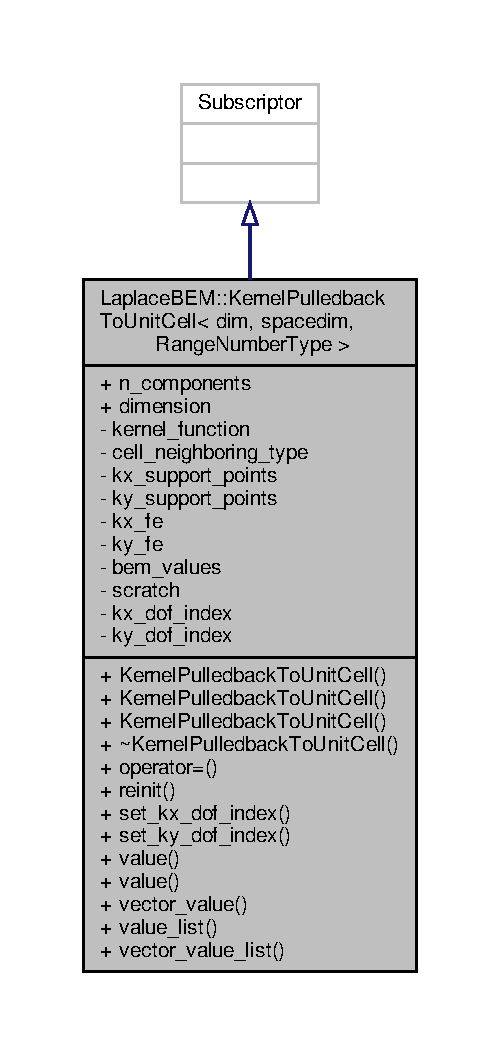
\includegraphics[width=240pt]{classLaplaceBEM_1_1KernelPulledbackToUnitCell__inherit__graph}
\end{center}
\end{figure}


Collaboration diagram for Laplace\+B\+EM\+:\+:Kernel\+Pulledback\+To\+Unit\+Cell$<$ dim, spacedim, Range\+Number\+Type $>$\+:\nopagebreak
\begin{figure}[H]
\begin{center}
\leavevmode
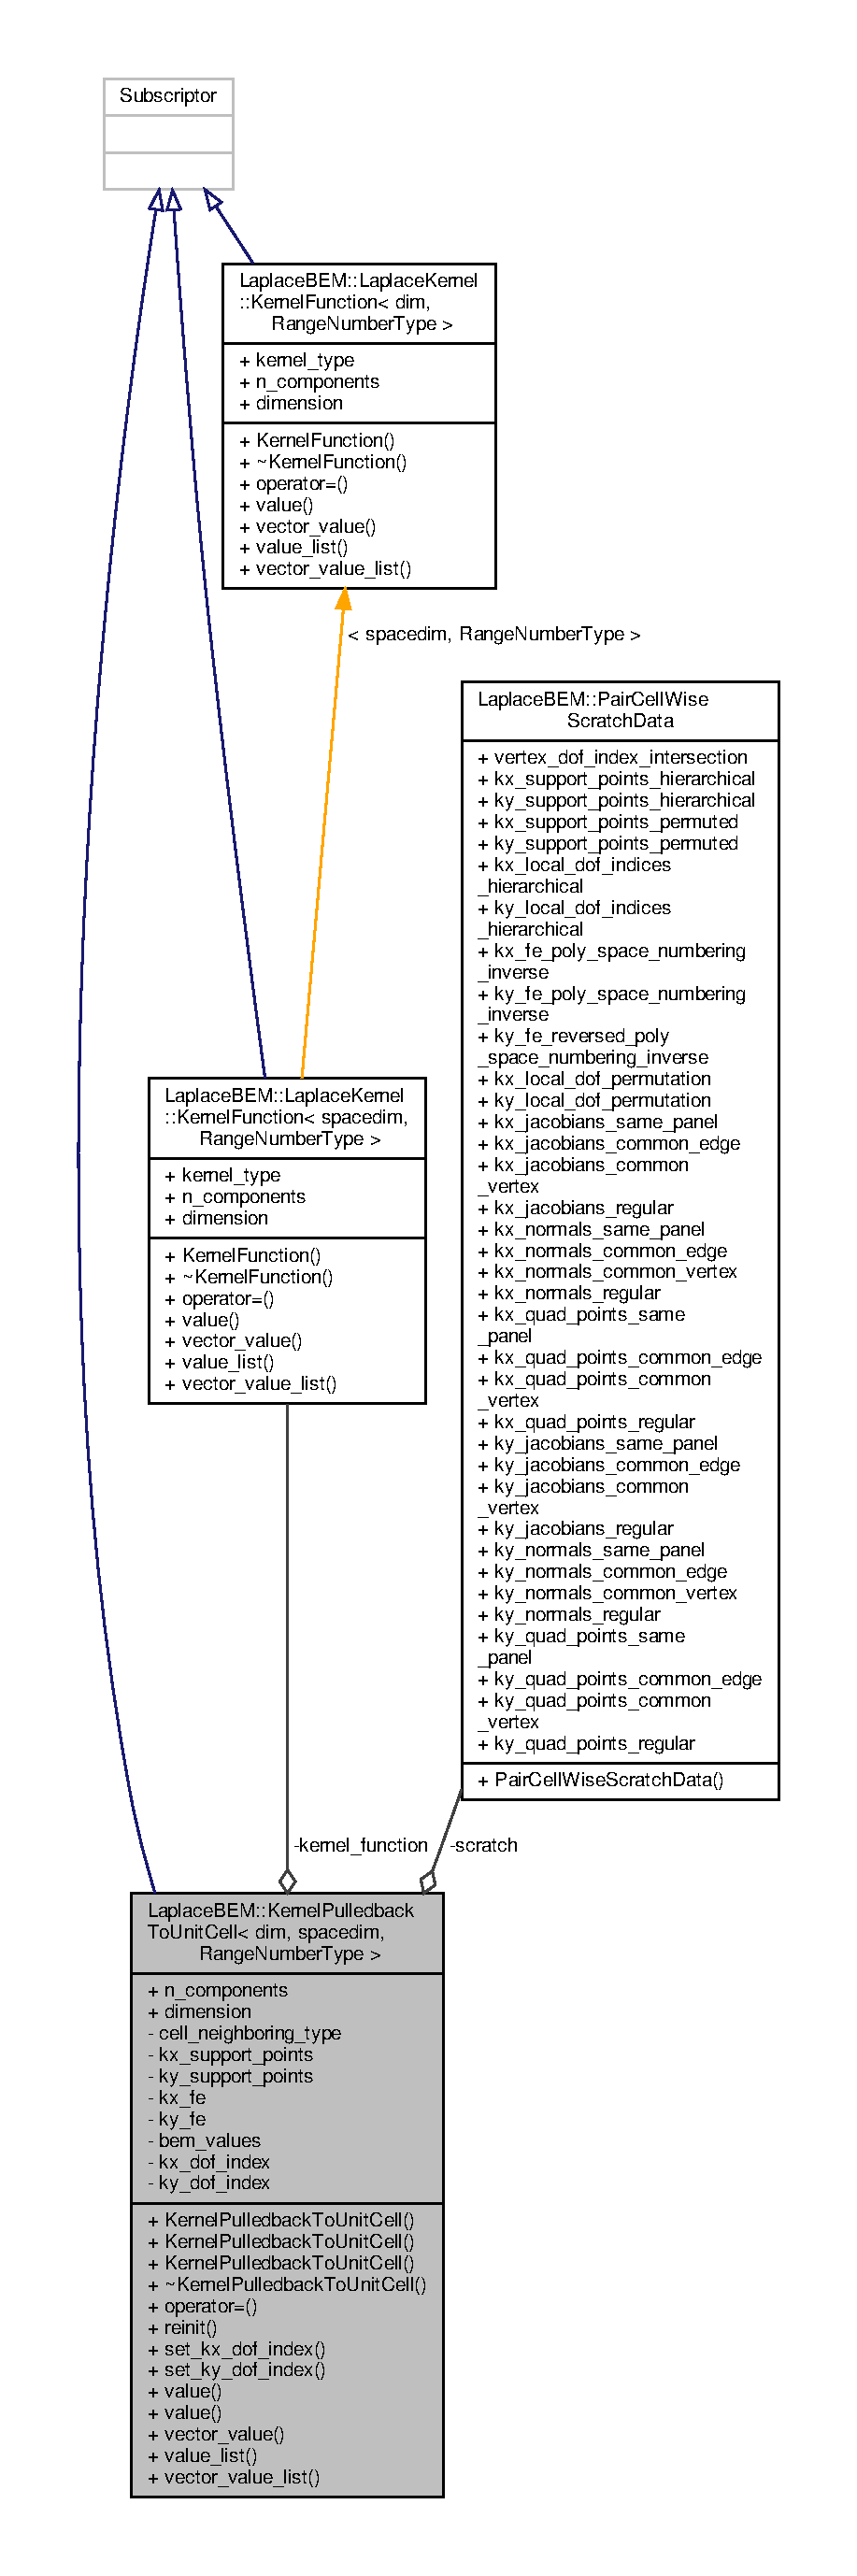
\includegraphics[height=550pt]{classLaplaceBEM_1_1KernelPulledbackToUnitCell__coll__graph}
\end{center}
\end{figure}
\subsection*{Public Member Functions}
\begin{DoxyCompactItemize}
\item 
\hyperlink{classLaplaceBEM_1_1KernelPulledbackToUnitCell_a344ad653c5e57498cc005b5b683e8db6}{Kernel\+Pulledback\+To\+Unit\+Cell} (const \hyperlink{classLaplaceBEM_1_1LaplaceKernel_1_1KernelFunction}{Laplace\+Kernel\+::\+Kernel\+Function}$<$ spacedim, Range\+Number\+Type $>$ \&kernel\+\_\+function, const Cell\+Neighboring\+Type \&cell\+\_\+neighboring\+\_\+type, const std\+::vector$<$ Point$<$ spacedim $>$$>$ \&kx\+\_\+support\+\_\+points, const std\+::vector$<$ Point$<$ spacedim $>$$>$ \&ky\+\_\+support\+\_\+points, const Finite\+Element$<$ dim, spacedim $>$ \&kx\+\_\+fe, const Finite\+Element$<$ dim, spacedim $>$ \&ky\+\_\+fe, const unsigned int \hyperlink{classLaplaceBEM_1_1KernelPulledbackToUnitCell_a66ba57ad86025978e5e5580c822aef89}{kx\+\_\+dof\+\_\+index}=0, const unsigned int \hyperlink{classLaplaceBEM_1_1KernelPulledbackToUnitCell_ae6f3e4bc6cf09546bf11d01812f9b692}{ky\+\_\+dof\+\_\+index}=0)
\item 
\hyperlink{classLaplaceBEM_1_1KernelPulledbackToUnitCell_a3ef9d5f4401cc8d6bd7c11955fadb770}{Kernel\+Pulledback\+To\+Unit\+Cell} (const \hyperlink{classLaplaceBEM_1_1LaplaceKernel_1_1KernelFunction}{Laplace\+Kernel\+::\+Kernel\+Function}$<$ spacedim, Range\+Number\+Type $>$ \&kernel\+\_\+function, const Cell\+Neighboring\+Type \&cell\+\_\+neighboring\+\_\+type, const std\+::vector$<$ Point$<$ spacedim $>$$>$ \&kx\+\_\+support\+\_\+points, const std\+::vector$<$ Point$<$ spacedim $>$$>$ \&ky\+\_\+support\+\_\+points, const Finite\+Element$<$ dim, spacedim $>$ \&kx\+\_\+fe, const Finite\+Element$<$ dim, spacedim $>$ \&ky\+\_\+fe, const \hyperlink{classLaplaceBEM_1_1BEMValues}{B\+E\+M\+Values}$<$ dim, spacedim, Range\+Number\+Type $>$ $\ast$bem\+\_\+values, const unsigned int \hyperlink{classLaplaceBEM_1_1KernelPulledbackToUnitCell_a66ba57ad86025978e5e5580c822aef89}{kx\+\_\+dof\+\_\+index}=0, const unsigned int \hyperlink{classLaplaceBEM_1_1KernelPulledbackToUnitCell_ae6f3e4bc6cf09546bf11d01812f9b692}{ky\+\_\+dof\+\_\+index}=0)
\item 
\hyperlink{classLaplaceBEM_1_1KernelPulledbackToUnitCell_afd01d1f6655a678124f2d0e3684b419d}{Kernel\+Pulledback\+To\+Unit\+Cell} (const \hyperlink{classLaplaceBEM_1_1LaplaceKernel_1_1KernelFunction}{Laplace\+Kernel\+::\+Kernel\+Function}$<$ spacedim, Range\+Number\+Type $>$ \&kernel\+\_\+function, const Cell\+Neighboring\+Type \&cell\+\_\+neighboring\+\_\+type, const std\+::vector$<$ Point$<$ spacedim $>$$>$ \&kx\+\_\+support\+\_\+points, const std\+::vector$<$ Point$<$ spacedim $>$$>$ \&ky\+\_\+support\+\_\+points, const Finite\+Element$<$ dim, spacedim $>$ \&kx\+\_\+fe, const Finite\+Element$<$ dim, spacedim $>$ \&ky\+\_\+fe, const \hyperlink{classLaplaceBEM_1_1BEMValues}{B\+E\+M\+Values}$<$ dim, spacedim, Range\+Number\+Type $>$ $\ast$bem\+\_\+values, const \hyperlink{structLaplaceBEM_1_1PairCellWiseScratchData}{Pair\+Cell\+Wise\+Scratch\+Data} $\ast$scratch, const unsigned int \hyperlink{classLaplaceBEM_1_1KernelPulledbackToUnitCell_a66ba57ad86025978e5e5580c822aef89}{kx\+\_\+dof\+\_\+index}=0, const unsigned int \hyperlink{classLaplaceBEM_1_1KernelPulledbackToUnitCell_ae6f3e4bc6cf09546bf11d01812f9b692}{ky\+\_\+dof\+\_\+index}=0)
\item 
\mbox{\Hypertarget{classLaplaceBEM_1_1KernelPulledbackToUnitCell_a1fd71ef63d7bd116cef37b5fe9189c40}\label{classLaplaceBEM_1_1KernelPulledbackToUnitCell_a1fd71ef63d7bd116cef37b5fe9189c40}} 
\hyperlink{classLaplaceBEM_1_1KernelPulledbackToUnitCell}{Kernel\+Pulledback\+To\+Unit\+Cell} \& {\bfseries operator=} (const \hyperlink{classLaplaceBEM_1_1KernelPulledbackToUnitCell}{Kernel\+Pulledback\+To\+Unit\+Cell} \&f)
\item 
void \hyperlink{classLaplaceBEM_1_1KernelPulledbackToUnitCell_a6c4063a68f9981ed1f2327670c512f59}{reinit} (const Cell\+Neighboring\+Type \&cell\+\_\+neighboring\+\_\+type, const std\+::vector$<$ Point$<$ spacedim $>$$>$ \&kx\+\_\+support\+\_\+points, const std\+::vector$<$ Point$<$ spacedim $>$$>$ \&ky\+\_\+support\+\_\+points, const Finite\+Element$<$ dim, spacedim $>$ \&kx\+\_\+fe, const Finite\+Element$<$ dim, spacedim $>$ \&ky\+\_\+fe)
\item 
\mbox{\Hypertarget{classLaplaceBEM_1_1KernelPulledbackToUnitCell_a1067e884c01a2f6d4648f9fc08fc2bc2}\label{classLaplaceBEM_1_1KernelPulledbackToUnitCell_a1067e884c01a2f6d4648f9fc08fc2bc2}} 
void {\bfseries set\+\_\+kx\+\_\+dof\+\_\+index} (const unsigned int \hyperlink{classLaplaceBEM_1_1KernelPulledbackToUnitCell_a66ba57ad86025978e5e5580c822aef89}{kx\+\_\+dof\+\_\+index})
\item 
\mbox{\Hypertarget{classLaplaceBEM_1_1KernelPulledbackToUnitCell_a39ea676a505803290a647c99699b5504}\label{classLaplaceBEM_1_1KernelPulledbackToUnitCell_a39ea676a505803290a647c99699b5504}} 
void {\bfseries set\+\_\+ky\+\_\+dof\+\_\+index} (const unsigned int \hyperlink{classLaplaceBEM_1_1KernelPulledbackToUnitCell_ae6f3e4bc6cf09546bf11d01812f9b692}{ky\+\_\+dof\+\_\+index})
\item 
virtual Range\+Number\+Type \hyperlink{classLaplaceBEM_1_1KernelPulledbackToUnitCell_ac55bd556acba999c6d71c322eff33cd9}{value} (const Point$<$ dim $>$ \&x\+\_\+hat, const Point$<$ dim $>$ \&y\+\_\+hat, const unsigned int component=0) const
\item 
\mbox{\Hypertarget{classLaplaceBEM_1_1KernelPulledbackToUnitCell_a72955834d5c6542c1f3216f408afe9f3}\label{classLaplaceBEM_1_1KernelPulledbackToUnitCell_a72955834d5c6542c1f3216f408afe9f3}} 
virtual Range\+Number\+Type {\bfseries value} (const unsigned int k3\+\_\+index, const unsigned int quad\+\_\+no, const unsigned int component=0) const
\item 
\mbox{\Hypertarget{classLaplaceBEM_1_1KernelPulledbackToUnitCell_aaea7ab071bb5a2fc03e7f613b0dabb57}\label{classLaplaceBEM_1_1KernelPulledbackToUnitCell_aaea7ab071bb5a2fc03e7f613b0dabb57}} 
virtual void {\bfseries vector\+\_\+value} (const Point$<$ dim $>$ \&x\+\_\+hat, const Point$<$ dim $>$ \&y\+\_\+hat, Vector$<$ Range\+Number\+Type $>$ \&values) const
\item 
\mbox{\Hypertarget{classLaplaceBEM_1_1KernelPulledbackToUnitCell_a73ddab1e4b36915991549a5476b8a803}\label{classLaplaceBEM_1_1KernelPulledbackToUnitCell_a73ddab1e4b36915991549a5476b8a803}} 
virtual void {\bfseries value\+\_\+list} (const std\+::vector$<$ Point$<$ dim $>$$>$ \&x\+\_\+hat\+\_\+list, const std\+::vector$<$ Point$<$ dim $>$$>$ \&y\+\_\+hat\+\_\+list, std\+::vector$<$ Range\+Number\+Type $>$ \&values, const unsigned int component=0) const
\item 
\mbox{\Hypertarget{classLaplaceBEM_1_1KernelPulledbackToUnitCell_a9aa5a715991470a7e8a69f40426d6cd9}\label{classLaplaceBEM_1_1KernelPulledbackToUnitCell_a9aa5a715991470a7e8a69f40426d6cd9}} 
virtual void {\bfseries vector\+\_\+value\+\_\+list} (const std\+::vector$<$ Point$<$ dim $>$$>$ \&x\+\_\+hat\+\_\+list, const std\+::vector$<$ Point$<$ dim $>$$>$ \&y\+\_\+hat\+\_\+list, std\+::vector$<$ Vector$<$ Range\+Number\+Type $>$$>$ \&values) const
\end{DoxyCompactItemize}
\subsection*{Public Attributes}
\begin{DoxyCompactItemize}
\item 
\mbox{\Hypertarget{classLaplaceBEM_1_1KernelPulledbackToUnitCell_ad351c9674e4bd484e5d5396210abe282}\label{classLaplaceBEM_1_1KernelPulledbackToUnitCell_ad351c9674e4bd484e5d5396210abe282}} 
const unsigned int {\bfseries n\+\_\+components}
\end{DoxyCompactItemize}
\subsection*{Static Public Attributes}
\begin{DoxyCompactItemize}
\item 
\mbox{\Hypertarget{classLaplaceBEM_1_1KernelPulledbackToUnitCell_a03ac8378093fac9ad01272ef619aa26e}\label{classLaplaceBEM_1_1KernelPulledbackToUnitCell_a03ac8378093fac9ad01272ef619aa26e}} 
static const unsigned int {\bfseries dimension} = dim
\end{DoxyCompactItemize}
\subsection*{Private Attributes}
\begin{DoxyCompactItemize}
\item 
\mbox{\Hypertarget{classLaplaceBEM_1_1KernelPulledbackToUnitCell_acf7e47b2ed819a2c6f320a306a2689fe}\label{classLaplaceBEM_1_1KernelPulledbackToUnitCell_acf7e47b2ed819a2c6f320a306a2689fe}} 
const \hyperlink{classLaplaceBEM_1_1LaplaceKernel_1_1KernelFunction}{Laplace\+Kernel\+::\+Kernel\+Function}$<$ spacedim, Range\+Number\+Type $>$ \& {\bfseries kernel\+\_\+function}
\item 
\mbox{\Hypertarget{classLaplaceBEM_1_1KernelPulledbackToUnitCell_a82662fdd33ceb50cd40aaf7b2bd1b32a}\label{classLaplaceBEM_1_1KernelPulledbackToUnitCell_a82662fdd33ceb50cd40aaf7b2bd1b32a}} 
Cell\+Neighboring\+Type {\bfseries cell\+\_\+neighboring\+\_\+type}
\item 
\mbox{\Hypertarget{classLaplaceBEM_1_1KernelPulledbackToUnitCell_ac7667f6cacebaed1a6ba39d67211db04}\label{classLaplaceBEM_1_1KernelPulledbackToUnitCell_ac7667f6cacebaed1a6ba39d67211db04}} 
const std\+::vector$<$ Point$<$ spacedim $>$ $>$ \& {\bfseries kx\+\_\+support\+\_\+points}
\item 
\mbox{\Hypertarget{classLaplaceBEM_1_1KernelPulledbackToUnitCell_a92971044a5f8ce2f61688858a3deac8e}\label{classLaplaceBEM_1_1KernelPulledbackToUnitCell_a92971044a5f8ce2f61688858a3deac8e}} 
const std\+::vector$<$ Point$<$ spacedim $>$ $>$ \& {\bfseries ky\+\_\+support\+\_\+points}
\item 
\mbox{\Hypertarget{classLaplaceBEM_1_1KernelPulledbackToUnitCell_a0455971a463de57f21930bb134461a17}\label{classLaplaceBEM_1_1KernelPulledbackToUnitCell_a0455971a463de57f21930bb134461a17}} 
const Finite\+Element$<$ dim, spacedim $>$ \& {\bfseries kx\+\_\+fe}
\item 
\mbox{\Hypertarget{classLaplaceBEM_1_1KernelPulledbackToUnitCell_a664dab9bbbf454f7636c61f43b4829eb}\label{classLaplaceBEM_1_1KernelPulledbackToUnitCell_a664dab9bbbf454f7636c61f43b4829eb}} 
const Finite\+Element$<$ dim, spacedim $>$ \& {\bfseries ky\+\_\+fe}
\item 
\mbox{\Hypertarget{classLaplaceBEM_1_1KernelPulledbackToUnitCell_a00b7c35e8a15b73113921af1eb3a3539}\label{classLaplaceBEM_1_1KernelPulledbackToUnitCell_a00b7c35e8a15b73113921af1eb3a3539}} 
const \hyperlink{classLaplaceBEM_1_1BEMValues}{B\+E\+M\+Values}$<$ dim, spacedim, Range\+Number\+Type $>$ $\ast$ {\bfseries bem\+\_\+values}
\item 
\mbox{\Hypertarget{classLaplaceBEM_1_1KernelPulledbackToUnitCell_a39328e6d06348a2a4841f91077ea2a6c}\label{classLaplaceBEM_1_1KernelPulledbackToUnitCell_a39328e6d06348a2a4841f91077ea2a6c}} 
const \hyperlink{structLaplaceBEM_1_1PairCellWiseScratchData}{Pair\+Cell\+Wise\+Scratch\+Data} $\ast$ {\bfseries scratch}
\item 
unsigned int \hyperlink{classLaplaceBEM_1_1KernelPulledbackToUnitCell_a66ba57ad86025978e5e5580c822aef89}{kx\+\_\+dof\+\_\+index}
\item 
unsigned int \hyperlink{classLaplaceBEM_1_1KernelPulledbackToUnitCell_ae6f3e4bc6cf09546bf11d01812f9b692}{ky\+\_\+dof\+\_\+index}
\end{DoxyCompactItemize}


\subsection{Detailed Description}
\subsubsection*{template$<$int dim, int spacedim, typename Range\+Number\+Type = double$>$\newline
class Laplace\+B\+E\+M\+::\+Kernel\+Pulledback\+To\+Unit\+Cell$<$ dim, spacedim, Range\+Number\+Type $>$}

Kernel function pulled back to unit cell. 

\subsection{Constructor \& Destructor Documentation}
\mbox{\Hypertarget{classLaplaceBEM_1_1KernelPulledbackToUnitCell_a344ad653c5e57498cc005b5b683e8db6}\label{classLaplaceBEM_1_1KernelPulledbackToUnitCell_a344ad653c5e57498cc005b5b683e8db6}} 
\index{Laplace\+B\+E\+M\+::\+Kernel\+Pulledback\+To\+Unit\+Cell@{Laplace\+B\+E\+M\+::\+Kernel\+Pulledback\+To\+Unit\+Cell}!Kernel\+Pulledback\+To\+Unit\+Cell@{Kernel\+Pulledback\+To\+Unit\+Cell}}
\index{Kernel\+Pulledback\+To\+Unit\+Cell@{Kernel\+Pulledback\+To\+Unit\+Cell}!Laplace\+B\+E\+M\+::\+Kernel\+Pulledback\+To\+Unit\+Cell@{Laplace\+B\+E\+M\+::\+Kernel\+Pulledback\+To\+Unit\+Cell}}
\subsubsection{\texorpdfstring{Kernel\+Pulledback\+To\+Unit\+Cell()}{KernelPulledbackToUnitCell()}\hspace{0.1cm}{\footnotesize\ttfamily [1/3]}}
{\footnotesize\ttfamily template$<$int dim, int spacedim, typename Range\+Number\+Type $>$ \\
\hyperlink{classLaplaceBEM_1_1KernelPulledbackToUnitCell}{Laplace\+B\+E\+M\+::\+Kernel\+Pulledback\+To\+Unit\+Cell}$<$ dim, spacedim, Range\+Number\+Type $>$\+::\hyperlink{classLaplaceBEM_1_1KernelPulledbackToUnitCell}{Kernel\+Pulledback\+To\+Unit\+Cell} (\begin{DoxyParamCaption}\item[{const \hyperlink{classLaplaceBEM_1_1LaplaceKernel_1_1KernelFunction}{Laplace\+Kernel\+::\+Kernel\+Function}$<$ spacedim, Range\+Number\+Type $>$ \&}]{kernel\+\_\+function,  }\item[{const Cell\+Neighboring\+Type \&}]{cell\+\_\+neighboring\+\_\+type,  }\item[{const std\+::vector$<$ Point$<$ spacedim $>$$>$ \&}]{kx\+\_\+support\+\_\+points,  }\item[{const std\+::vector$<$ Point$<$ spacedim $>$$>$ \&}]{ky\+\_\+support\+\_\+points,  }\item[{const Finite\+Element$<$ dim, spacedim $>$ \&}]{kx\+\_\+fe,  }\item[{const Finite\+Element$<$ dim, spacedim $>$ \&}]{ky\+\_\+fe,  }\item[{const unsigned int}]{kx\+\_\+dof\+\_\+index = {\ttfamily 0},  }\item[{const unsigned int}]{ky\+\_\+dof\+\_\+index = {\ttfamily 0} }\end{DoxyParamCaption})}

Constructor for \hyperlink{classLaplaceBEM_1_1KernelPulledbackToUnitCell}{Kernel\+Pulledback\+To\+Unit\+Cell}.


\begin{DoxyParams}{Parameters}
{\em kx\+\_\+support\+\_\+points} & Permuted list of support points in \$\+K\+\_\+x\$. \\
\hline
{\em ky\+\_\+support\+\_\+points} & Permuted list of support points in \$\+K\+\_\+y\$. \\
\hline
{\em kx\+\_\+dof\+\_\+index} & Index for accessing the list of Do\+Fs in tensor product order in \$\+K\+\_\+x\$. \\
\hline
{\em ky\+\_\+dof\+\_\+index} & Index for accessing the list of Do\+Fs in tensor product order in \$\+K\+\_\+y\$. \\
\hline
\end{DoxyParams}


Referenced by Laplace\+B\+E\+M\+::\+Kernel\+Pulledback\+To\+Unit\+Cell$<$ dim, spacedim, Range\+Number\+Type $>$\+::\+Kernel\+Pulledback\+To\+Unit\+Cell().

\mbox{\Hypertarget{classLaplaceBEM_1_1KernelPulledbackToUnitCell_a3ef9d5f4401cc8d6bd7c11955fadb770}\label{classLaplaceBEM_1_1KernelPulledbackToUnitCell_a3ef9d5f4401cc8d6bd7c11955fadb770}} 
\index{Laplace\+B\+E\+M\+::\+Kernel\+Pulledback\+To\+Unit\+Cell@{Laplace\+B\+E\+M\+::\+Kernel\+Pulledback\+To\+Unit\+Cell}!Kernel\+Pulledback\+To\+Unit\+Cell@{Kernel\+Pulledback\+To\+Unit\+Cell}}
\index{Kernel\+Pulledback\+To\+Unit\+Cell@{Kernel\+Pulledback\+To\+Unit\+Cell}!Laplace\+B\+E\+M\+::\+Kernel\+Pulledback\+To\+Unit\+Cell@{Laplace\+B\+E\+M\+::\+Kernel\+Pulledback\+To\+Unit\+Cell}}
\subsubsection{\texorpdfstring{Kernel\+Pulledback\+To\+Unit\+Cell()}{KernelPulledbackToUnitCell()}\hspace{0.1cm}{\footnotesize\ttfamily [2/3]}}
{\footnotesize\ttfamily template$<$int dim, int spacedim, typename Range\+Number\+Type $>$ \\
\hyperlink{classLaplaceBEM_1_1KernelPulledbackToUnitCell}{Laplace\+B\+E\+M\+::\+Kernel\+Pulledback\+To\+Unit\+Cell}$<$ dim, spacedim, Range\+Number\+Type $>$\+::\hyperlink{classLaplaceBEM_1_1KernelPulledbackToUnitCell}{Kernel\+Pulledback\+To\+Unit\+Cell} (\begin{DoxyParamCaption}\item[{const \hyperlink{classLaplaceBEM_1_1LaplaceKernel_1_1KernelFunction}{Laplace\+Kernel\+::\+Kernel\+Function}$<$ spacedim, Range\+Number\+Type $>$ \&}]{kernel\+\_\+function,  }\item[{const Cell\+Neighboring\+Type \&}]{cell\+\_\+neighboring\+\_\+type,  }\item[{const std\+::vector$<$ Point$<$ spacedim $>$$>$ \&}]{kx\+\_\+support\+\_\+points,  }\item[{const std\+::vector$<$ Point$<$ spacedim $>$$>$ \&}]{ky\+\_\+support\+\_\+points,  }\item[{const Finite\+Element$<$ dim, spacedim $>$ \&}]{kx\+\_\+fe,  }\item[{const Finite\+Element$<$ dim, spacedim $>$ \&}]{ky\+\_\+fe,  }\item[{const \hyperlink{classLaplaceBEM_1_1BEMValues}{B\+E\+M\+Values}$<$ dim, spacedim, Range\+Number\+Type $>$ $\ast$}]{bem\+\_\+values,  }\item[{const unsigned int}]{kx\+\_\+dof\+\_\+index = {\ttfamily 0},  }\item[{const unsigned int}]{ky\+\_\+dof\+\_\+index = {\ttfamily 0} }\end{DoxyParamCaption})}


\begin{DoxyParams}{Parameters}
{\em kernel\+\_\+function} & \\
\hline
{\em cell\+\_\+neighboring\+\_\+type} & \\
\hline
{\em kx\+\_\+support\+\_\+points} & \\
\hline
{\em ky\+\_\+support\+\_\+points} & \\
\hline
{\em kx\+\_\+fe} & \\
\hline
{\em ky\+\_\+fe} & \\
\hline
{\em bem\+\_\+values} & \\
\hline
{\em kx\+\_\+dof\+\_\+index} & \\
\hline
{\em ky\+\_\+dof\+\_\+index} & \\
\hline
\end{DoxyParams}


References Laplace\+B\+E\+M\+::\+Kernel\+Pulledback\+To\+Unit\+Cell$<$ dim, spacedim, Range\+Number\+Type $>$\+::\+Kernel\+Pulledback\+To\+Unit\+Cell().

\mbox{\Hypertarget{classLaplaceBEM_1_1KernelPulledbackToUnitCell_afd01d1f6655a678124f2d0e3684b419d}\label{classLaplaceBEM_1_1KernelPulledbackToUnitCell_afd01d1f6655a678124f2d0e3684b419d}} 
\index{Laplace\+B\+E\+M\+::\+Kernel\+Pulledback\+To\+Unit\+Cell@{Laplace\+B\+E\+M\+::\+Kernel\+Pulledback\+To\+Unit\+Cell}!Kernel\+Pulledback\+To\+Unit\+Cell@{Kernel\+Pulledback\+To\+Unit\+Cell}}
\index{Kernel\+Pulledback\+To\+Unit\+Cell@{Kernel\+Pulledback\+To\+Unit\+Cell}!Laplace\+B\+E\+M\+::\+Kernel\+Pulledback\+To\+Unit\+Cell@{Laplace\+B\+E\+M\+::\+Kernel\+Pulledback\+To\+Unit\+Cell}}
\subsubsection{\texorpdfstring{Kernel\+Pulledback\+To\+Unit\+Cell()}{KernelPulledbackToUnitCell()}\hspace{0.1cm}{\footnotesize\ttfamily [3/3]}}
{\footnotesize\ttfamily template$<$int dim, int spacedim, typename Range\+Number\+Type $>$ \\
\hyperlink{classLaplaceBEM_1_1KernelPulledbackToUnitCell}{Laplace\+B\+E\+M\+::\+Kernel\+Pulledback\+To\+Unit\+Cell}$<$ dim, spacedim, Range\+Number\+Type $>$\+::\hyperlink{classLaplaceBEM_1_1KernelPulledbackToUnitCell}{Kernel\+Pulledback\+To\+Unit\+Cell} (\begin{DoxyParamCaption}\item[{const \hyperlink{classLaplaceBEM_1_1LaplaceKernel_1_1KernelFunction}{Laplace\+Kernel\+::\+Kernel\+Function}$<$ spacedim, Range\+Number\+Type $>$ \&}]{kernel\+\_\+function,  }\item[{const Cell\+Neighboring\+Type \&}]{cell\+\_\+neighboring\+\_\+type,  }\item[{const std\+::vector$<$ Point$<$ spacedim $>$$>$ \&}]{kx\+\_\+support\+\_\+points,  }\item[{const std\+::vector$<$ Point$<$ spacedim $>$$>$ \&}]{ky\+\_\+support\+\_\+points,  }\item[{const Finite\+Element$<$ dim, spacedim $>$ \&}]{kx\+\_\+fe,  }\item[{const Finite\+Element$<$ dim, spacedim $>$ \&}]{ky\+\_\+fe,  }\item[{const \hyperlink{classLaplaceBEM_1_1BEMValues}{B\+E\+M\+Values}$<$ dim, spacedim, Range\+Number\+Type $>$ $\ast$}]{bem\+\_\+values,  }\item[{const \hyperlink{structLaplaceBEM_1_1PairCellWiseScratchData}{Pair\+Cell\+Wise\+Scratch\+Data} $\ast$}]{scratch,  }\item[{const unsigned int}]{kx\+\_\+dof\+\_\+index = {\ttfamily 0},  }\item[{const unsigned int}]{ky\+\_\+dof\+\_\+index = {\ttfamily 0} }\end{DoxyParamCaption})}


\begin{DoxyParams}{Parameters}
{\em kernel\+\_\+function} & \\
\hline
{\em cell\+\_\+neighboring\+\_\+type} & \\
\hline
{\em kx\+\_\+support\+\_\+points} & \\
\hline
{\em ky\+\_\+support\+\_\+points} & \\
\hline
{\em kx\+\_\+fe} & \\
\hline
{\em ky\+\_\+fe} & \\
\hline
{\em bem\+\_\+values} & \\
\hline
{\em kx\+\_\+dof\+\_\+index} & \\
\hline
{\em ky\+\_\+dof\+\_\+index} & \\
\hline
\end{DoxyParams}


\subsection{Member Function Documentation}
\mbox{\Hypertarget{classLaplaceBEM_1_1KernelPulledbackToUnitCell_a6c4063a68f9981ed1f2327670c512f59}\label{classLaplaceBEM_1_1KernelPulledbackToUnitCell_a6c4063a68f9981ed1f2327670c512f59}} 
\index{Laplace\+B\+E\+M\+::\+Kernel\+Pulledback\+To\+Unit\+Cell@{Laplace\+B\+E\+M\+::\+Kernel\+Pulledback\+To\+Unit\+Cell}!reinit@{reinit}}
\index{reinit@{reinit}!Laplace\+B\+E\+M\+::\+Kernel\+Pulledback\+To\+Unit\+Cell@{Laplace\+B\+E\+M\+::\+Kernel\+Pulledback\+To\+Unit\+Cell}}
\subsubsection{\texorpdfstring{reinit()}{reinit()}}
{\footnotesize\ttfamily template$<$int dim, int spacedim, typename Range\+Number\+Type $>$ \\
void \hyperlink{classLaplaceBEM_1_1KernelPulledbackToUnitCell}{Laplace\+B\+E\+M\+::\+Kernel\+Pulledback\+To\+Unit\+Cell}$<$ dim, spacedim, Range\+Number\+Type $>$\+::reinit (\begin{DoxyParamCaption}\item[{const Cell\+Neighboring\+Type \&}]{cell\+\_\+neighboring\+\_\+type,  }\item[{const std\+::vector$<$ Point$<$ spacedim $>$$>$ \&}]{kx\+\_\+support\+\_\+points,  }\item[{const std\+::vector$<$ Point$<$ spacedim $>$$>$ \&}]{ky\+\_\+support\+\_\+points,  }\item[{const Finite\+Element$<$ dim, spacedim $>$ \&}]{kx\+\_\+fe,  }\item[{const Finite\+Element$<$ dim, spacedim $>$ \&}]{ky\+\_\+fe }\end{DoxyParamCaption})}

Associate the \hyperlink{classLaplaceBEM_1_1KernelPulledbackToUnitCell}{Kernel\+Pulledback\+To\+Unit\+Cell} with new support point and finite element data. 

References Laplace\+B\+E\+M\+::\+Kernel\+Pulledback\+To\+Unit\+Cell$<$ dim, spacedim, Range\+Number\+Type $>$\+::kx\+\_\+dof\+\_\+index, and Laplace\+B\+E\+M\+::\+Kernel\+Pulledback\+To\+Unit\+Cell$<$ dim, spacedim, Range\+Number\+Type $>$\+::ky\+\_\+dof\+\_\+index.

\mbox{\Hypertarget{classLaplaceBEM_1_1KernelPulledbackToUnitCell_ac55bd556acba999c6d71c322eff33cd9}\label{classLaplaceBEM_1_1KernelPulledbackToUnitCell_ac55bd556acba999c6d71c322eff33cd9}} 
\index{Laplace\+B\+E\+M\+::\+Kernel\+Pulledback\+To\+Unit\+Cell@{Laplace\+B\+E\+M\+::\+Kernel\+Pulledback\+To\+Unit\+Cell}!value@{value}}
\index{value@{value}!Laplace\+B\+E\+M\+::\+Kernel\+Pulledback\+To\+Unit\+Cell@{Laplace\+B\+E\+M\+::\+Kernel\+Pulledback\+To\+Unit\+Cell}}
\subsubsection{\texorpdfstring{value()}{value()}}
{\footnotesize\ttfamily template$<$int dim, int spacedim, typename Range\+Number\+Type $>$ \\
Range\+Number\+Type \hyperlink{classLaplaceBEM_1_1KernelPulledbackToUnitCell}{Laplace\+B\+E\+M\+::\+Kernel\+Pulledback\+To\+Unit\+Cell}$<$ dim, spacedim, Range\+Number\+Type $>$\+::value (\begin{DoxyParamCaption}\item[{const Point$<$ dim $>$ \&}]{x\+\_\+hat,  }\item[{const Point$<$ dim $>$ \&}]{y\+\_\+hat,  }\item[{const unsigned int}]{component = {\ttfamily 0} }\end{DoxyParamCaption}) const\hspace{0.3cm}{\ttfamily [virtual]}}

Evaluation of the function which depends on the kernel type. Different types of kernel function require different normal vector data. 

References Laplace\+B\+E\+M\+::transform\+\_\+unit\+\_\+to\+\_\+permuted\+\_\+real\+\_\+cell().



\subsection{Member Data Documentation}
\mbox{\Hypertarget{classLaplaceBEM_1_1KernelPulledbackToUnitCell_a66ba57ad86025978e5e5580c822aef89}\label{classLaplaceBEM_1_1KernelPulledbackToUnitCell_a66ba57ad86025978e5e5580c822aef89}} 
\index{Laplace\+B\+E\+M\+::\+Kernel\+Pulledback\+To\+Unit\+Cell@{Laplace\+B\+E\+M\+::\+Kernel\+Pulledback\+To\+Unit\+Cell}!kx\+\_\+dof\+\_\+index@{kx\+\_\+dof\+\_\+index}}
\index{kx\+\_\+dof\+\_\+index@{kx\+\_\+dof\+\_\+index}!Laplace\+B\+E\+M\+::\+Kernel\+Pulledback\+To\+Unit\+Cell@{Laplace\+B\+E\+M\+::\+Kernel\+Pulledback\+To\+Unit\+Cell}}
\subsubsection{\texorpdfstring{kx\+\_\+dof\+\_\+index}{kx\_dof\_index}}
{\footnotesize\ttfamily template$<$int dim, int spacedim, typename Range\+Number\+Type = double$>$ \\
unsigned int \hyperlink{classLaplaceBEM_1_1KernelPulledbackToUnitCell}{Laplace\+B\+E\+M\+::\+Kernel\+Pulledback\+To\+Unit\+Cell}$<$ dim, spacedim, Range\+Number\+Type $>$\+::kx\+\_\+dof\+\_\+index\hspace{0.3cm}{\ttfamily [private]}}

Index for accessing the list of Do\+Fs in tensor product order in \$\+K\+\_\+x\$. 

Referenced by Laplace\+B\+E\+M\+::\+Kernel\+Pulledback\+To\+Unit\+Cell$<$ dim, spacedim, Range\+Number\+Type $>$\+::reinit().

\mbox{\Hypertarget{classLaplaceBEM_1_1KernelPulledbackToUnitCell_ae6f3e4bc6cf09546bf11d01812f9b692}\label{classLaplaceBEM_1_1KernelPulledbackToUnitCell_ae6f3e4bc6cf09546bf11d01812f9b692}} 
\index{Laplace\+B\+E\+M\+::\+Kernel\+Pulledback\+To\+Unit\+Cell@{Laplace\+B\+E\+M\+::\+Kernel\+Pulledback\+To\+Unit\+Cell}!ky\+\_\+dof\+\_\+index@{ky\+\_\+dof\+\_\+index}}
\index{ky\+\_\+dof\+\_\+index@{ky\+\_\+dof\+\_\+index}!Laplace\+B\+E\+M\+::\+Kernel\+Pulledback\+To\+Unit\+Cell@{Laplace\+B\+E\+M\+::\+Kernel\+Pulledback\+To\+Unit\+Cell}}
\subsubsection{\texorpdfstring{ky\+\_\+dof\+\_\+index}{ky\_dof\_index}}
{\footnotesize\ttfamily template$<$int dim, int spacedim, typename Range\+Number\+Type = double$>$ \\
unsigned int \hyperlink{classLaplaceBEM_1_1KernelPulledbackToUnitCell}{Laplace\+B\+E\+M\+::\+Kernel\+Pulledback\+To\+Unit\+Cell}$<$ dim, spacedim, Range\+Number\+Type $>$\+::ky\+\_\+dof\+\_\+index\hspace{0.3cm}{\ttfamily [private]}}

Index for accessing the list of Do\+Fs in tensor product order in \$\+K\+\_\+y\$. 

Referenced by Laplace\+B\+E\+M\+::\+Kernel\+Pulledback\+To\+Unit\+Cell$<$ dim, spacedim, Range\+Number\+Type $>$\+::reinit().



The documentation for this class was generated from the following file\+:\begin{DoxyCompactItemize}
\item 
/home/jihuan/\+Projects/deal.\+ii/program/dealii-\/9.\+1.\+1/examples/laplace-\/bem/include/\hyperlink{laplace__bem_8h}{laplace\+\_\+bem.\+h}\end{DoxyCompactItemize}

\hypertarget{classLAPACKFullMatrixExt}{}\section{L\+A\+P\+A\+C\+K\+Full\+Matrix\+Ext$<$ Number $>$ Class Template Reference}
\label{classLAPACKFullMatrixExt}\index{L\+A\+P\+A\+C\+K\+Full\+Matrix\+Ext$<$ Number $>$@{L\+A\+P\+A\+C\+K\+Full\+Matrix\+Ext$<$ Number $>$}}


{\ttfamily \#include $<$lapack\+\_\+full\+\_\+matrix\+\_\+ext.\+h$>$}



Inheritance diagram for L\+A\+P\+A\+C\+K\+Full\+Matrix\+Ext$<$ Number $>$\+:\nopagebreak
\begin{figure}[H]
\begin{center}
\leavevmode
\includegraphics[height=550pt]{classLAPACKFullMatrixExt__inherit__graph}
\end{center}
\end{figure}


Collaboration diagram for L\+A\+P\+A\+C\+K\+Full\+Matrix\+Ext$<$ Number $>$\+:\nopagebreak
\begin{figure}[H]
\begin{center}
\leavevmode
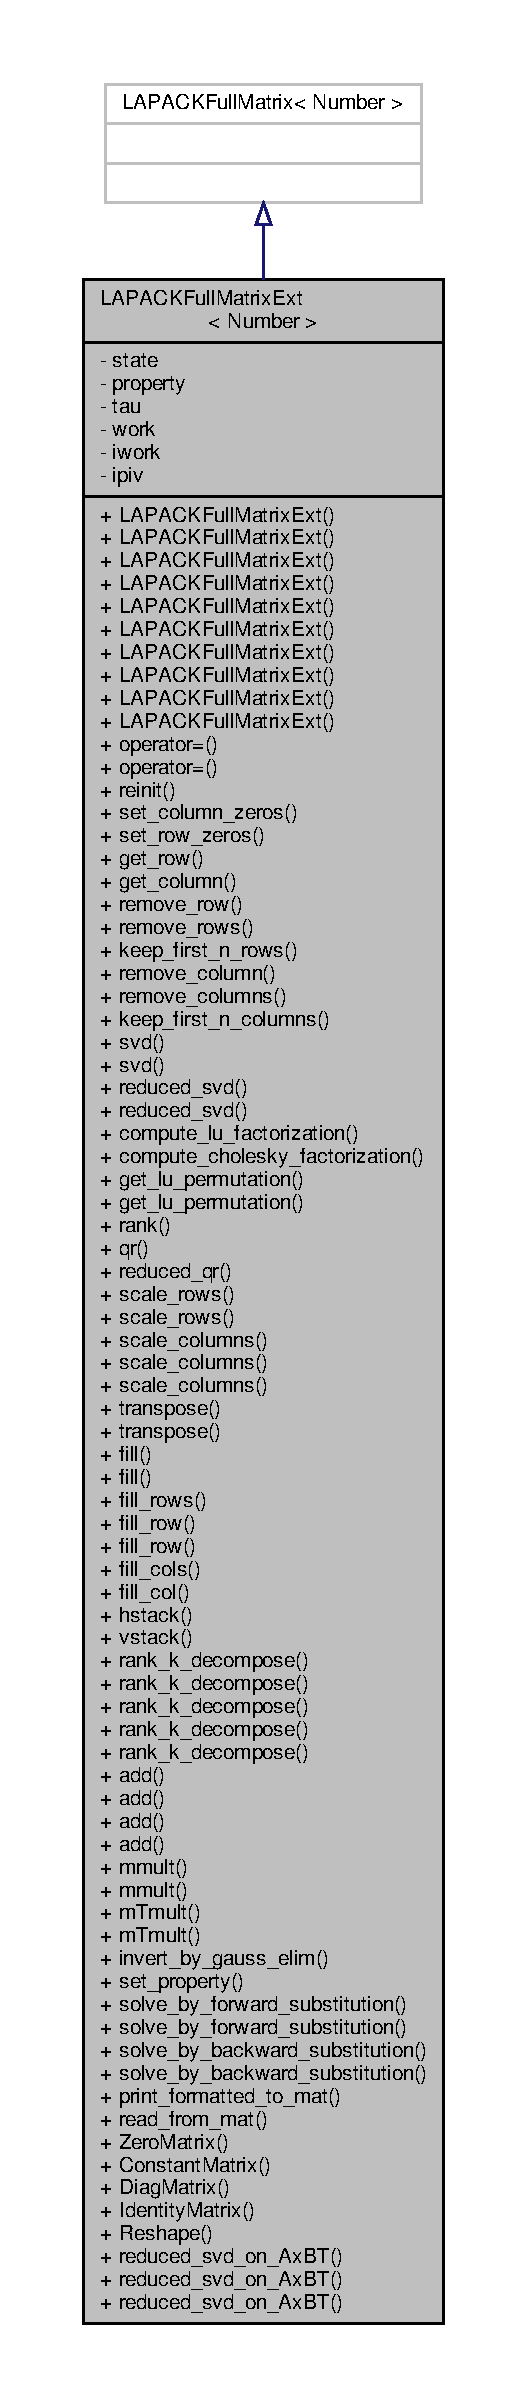
\includegraphics[height=550pt]{classLAPACKFullMatrixExt__coll__graph}
\end{center}
\end{figure}
\subsection*{Public Types}
\begin{DoxyCompactItemize}
\item 
using \hyperlink{classLAPACKFullMatrixExt_a5cf5f4a6104dc17029210b5ca52bf574}{size\+\_\+type} = std\+::make\+\_\+unsigned$<$ types\+::blas\+\_\+int $>$\+::type
\end{DoxyCompactItemize}
\subsection*{Public Member Functions}
\begin{DoxyCompactItemize}
\item 
\hyperlink{classLAPACKFullMatrixExt_a1d2edf7f0eb1f079e1d9540f89b6584e}{L\+A\+P\+A\+C\+K\+Full\+Matrix\+Ext} (const \hyperlink{classLAPACKFullMatrixExt_a5cf5f4a6104dc17029210b5ca52bf574}{size\+\_\+type} size=0)
\item 
\hyperlink{classLAPACKFullMatrixExt_a82986acedd4e702133151cb9a3ae2c97}{L\+A\+P\+A\+C\+K\+Full\+Matrix\+Ext} (const \hyperlink{classLAPACKFullMatrixExt_a5cf5f4a6104dc17029210b5ca52bf574}{size\+\_\+type} rows, const \hyperlink{classLAPACKFullMatrixExt_a5cf5f4a6104dc17029210b5ca52bf574}{size\+\_\+type} cols)
\item 
\hyperlink{classLAPACKFullMatrixExt_a95c6843f5138c51aa42b554ec843b717}{L\+A\+P\+A\+C\+K\+Full\+Matrix\+Ext} (const \hyperlink{classLAPACKFullMatrixExt}{L\+A\+P\+A\+C\+K\+Full\+Matrix\+Ext} \&mat)
\item 
\hyperlink{classLAPACKFullMatrixExt_adfb752e5770370e4f7ddbd298d873c60}{L\+A\+P\+A\+C\+K\+Full\+Matrix\+Ext} (const L\+A\+P\+A\+C\+K\+Full\+Matrix$<$ Number $>$ \&mat)
\item 
\hyperlink{classLAPACKFullMatrixExt_adcc17e75248175c5d89ba15ee58be954}{L\+A\+P\+A\+C\+K\+Full\+Matrix\+Ext} (const std\+::vector$<$ types\+::global\+\_\+dof\+\_\+index $>$ \&tau\+\_\+index\+\_\+set, const std\+::vector$<$ types\+::global\+\_\+dof\+\_\+index $>$ \&sigma\+\_\+index\+\_\+set, const \hyperlink{classLAPACKFullMatrixExt}{L\+A\+P\+A\+C\+K\+Full\+Matrix\+Ext}$<$ Number $>$ \&M)
\item 
\hyperlink{classLAPACKFullMatrixExt_a6ffdb7d0e8168100762813185480fb10}{L\+A\+P\+A\+C\+K\+Full\+Matrix\+Ext} (const std\+::vector$<$ types\+::global\+\_\+dof\+\_\+index $>$ \&tau\+\_\+index\+\_\+set, const std\+::vector$<$ types\+::global\+\_\+dof\+\_\+index $>$ \&sigma\+\_\+index\+\_\+set, const \hyperlink{classLAPACKFullMatrixExt}{L\+A\+P\+A\+C\+K\+Full\+Matrix\+Ext}$<$ Number $>$ \&M, const std\+::map$<$ types\+::global\+\_\+dof\+\_\+index, size\+\_\+t $>$ \&row\+\_\+index\+\_\+global\+\_\+to\+\_\+local\+\_\+map\+\_\+for\+\_\+M, const std\+::map$<$ types\+::global\+\_\+dof\+\_\+index, size\+\_\+t $>$ \&col\+\_\+index\+\_\+global\+\_\+to\+\_\+local\+\_\+map\+\_\+for\+\_\+M)
\item 
\hyperlink{classLAPACKFullMatrixExt_a98851864591035df275caca76e07ebe3}{L\+A\+P\+A\+C\+K\+Full\+Matrix\+Ext} (const \hyperlink{classLAPACKFullMatrixExt}{L\+A\+P\+A\+C\+K\+Full\+Matrix\+Ext} \&M1, const \hyperlink{classLAPACKFullMatrixExt}{L\+A\+P\+A\+C\+K\+Full\+Matrix\+Ext} \&M2, bool is\+\_\+horizontal\+\_\+split)
\item 
\hyperlink{classLAPACKFullMatrixExt_a1c8c9c59c2edc349031c4867c19067ef}{L\+A\+P\+A\+C\+K\+Full\+Matrix\+Ext} (const std\+::map$<$ types\+::global\+\_\+dof\+\_\+index, size\+\_\+t $>$ \&row\+\_\+index\+\_\+global\+\_\+to\+\_\+local\+\_\+map\+\_\+for\+\_\+M, const std\+::map$<$ types\+::global\+\_\+dof\+\_\+index, size\+\_\+t $>$ \&col\+\_\+index\+\_\+global\+\_\+to\+\_\+local\+\_\+map\+\_\+for\+\_\+M, const \hyperlink{classLAPACKFullMatrixExt}{L\+A\+P\+A\+C\+K\+Full\+Matrix\+Ext} \&M1, const std\+::vector$<$ types\+::global\+\_\+dof\+\_\+index $>$ \&M1\+\_\+tau\+\_\+index\+\_\+set, const std\+::vector$<$ types\+::global\+\_\+dof\+\_\+index $>$ \&M1\+\_\+sigma\+\_\+index\+\_\+set, const \hyperlink{classLAPACKFullMatrixExt}{L\+A\+P\+A\+C\+K\+Full\+Matrix\+Ext} \&M2, const std\+::vector$<$ types\+::global\+\_\+dof\+\_\+index $>$ \&M2\+\_\+tau\+\_\+index\+\_\+set, const std\+::vector$<$ types\+::global\+\_\+dof\+\_\+index $>$ \&M2\+\_\+sigma\+\_\+index\+\_\+set, bool is\+\_\+horizontal\+\_\+split)
\item 
\hyperlink{classLAPACKFullMatrixExt_aa94c466249d0df9e122443c0b6263cf3}{L\+A\+P\+A\+C\+K\+Full\+Matrix\+Ext} (const \hyperlink{classLAPACKFullMatrixExt}{L\+A\+P\+A\+C\+K\+Full\+Matrix\+Ext} \&M11, const \hyperlink{classLAPACKFullMatrixExt}{L\+A\+P\+A\+C\+K\+Full\+Matrix\+Ext} \&M12, const \hyperlink{classLAPACKFullMatrixExt}{L\+A\+P\+A\+C\+K\+Full\+Matrix\+Ext} \&M21, const \hyperlink{classLAPACKFullMatrixExt}{L\+A\+P\+A\+C\+K\+Full\+Matrix\+Ext} \&M22)
\item 
\hyperlink{classLAPACKFullMatrixExt_a4baa5d6642259df28cf9f32cb6b71a25}{L\+A\+P\+A\+C\+K\+Full\+Matrix\+Ext} (const std\+::map$<$ types\+::global\+\_\+dof\+\_\+index, size\+\_\+t $>$ \&row\+\_\+index\+\_\+global\+\_\+to\+\_\+local\+\_\+map\+\_\+for\+\_\+M, const std\+::map$<$ types\+::global\+\_\+dof\+\_\+index, size\+\_\+t $>$ \&col\+\_\+index\+\_\+global\+\_\+to\+\_\+local\+\_\+map\+\_\+for\+\_\+M, const \hyperlink{classLAPACKFullMatrixExt}{L\+A\+P\+A\+C\+K\+Full\+Matrix\+Ext} \&M11, const std\+::vector$<$ types\+::global\+\_\+dof\+\_\+index $>$ \&M11\+\_\+tau\+\_\+index\+\_\+set, const std\+::vector$<$ types\+::global\+\_\+dof\+\_\+index $>$ \&M11\+\_\+sigma\+\_\+index\+\_\+set, const \hyperlink{classLAPACKFullMatrixExt}{L\+A\+P\+A\+C\+K\+Full\+Matrix\+Ext} \&M12, const std\+::vector$<$ types\+::global\+\_\+dof\+\_\+index $>$ \&M12\+\_\+tau\+\_\+index\+\_\+set, const std\+::vector$<$ types\+::global\+\_\+dof\+\_\+index $>$ \&M12\+\_\+sigma\+\_\+index\+\_\+set, const \hyperlink{classLAPACKFullMatrixExt}{L\+A\+P\+A\+C\+K\+Full\+Matrix\+Ext} \&M21, const std\+::vector$<$ types\+::global\+\_\+dof\+\_\+index $>$ \&M21\+\_\+tau\+\_\+index\+\_\+set, const std\+::vector$<$ types\+::global\+\_\+dof\+\_\+index $>$ \&M21\+\_\+sigma\+\_\+index\+\_\+set, const \hyperlink{classLAPACKFullMatrixExt}{L\+A\+P\+A\+C\+K\+Full\+Matrix\+Ext} \&M22, const std\+::vector$<$ types\+::global\+\_\+dof\+\_\+index $>$ \&M22\+\_\+tau\+\_\+index\+\_\+set, const std\+::vector$<$ types\+::global\+\_\+dof\+\_\+index $>$ \&M22\+\_\+sigma\+\_\+index\+\_\+set)
\item 
\hyperlink{classLAPACKFullMatrixExt}{L\+A\+P\+A\+C\+K\+Full\+Matrix\+Ext}$<$ Number $>$ \& \hyperlink{classLAPACKFullMatrixExt_a48a8520d322ba5be9f5bb38e67f9b01b}{operator=} (const \hyperlink{classLAPACKFullMatrixExt}{L\+A\+P\+A\+C\+K\+Full\+Matrix\+Ext}$<$ Number $>$ \&matrix)
\item 
\hyperlink{classLAPACKFullMatrixExt}{L\+A\+P\+A\+C\+K\+Full\+Matrix\+Ext}$<$ Number $>$ \& \hyperlink{classLAPACKFullMatrixExt_ae277e753101db17ebf5bbd43dd04ab27}{operator=} (const L\+A\+P\+A\+C\+K\+Full\+Matrix$<$ Number $>$ \&matrix)
\item 
\mbox{\Hypertarget{classLAPACKFullMatrixExt_ae67c72d9ba641f02dc0e3b3486b95a10}\label{classLAPACKFullMatrixExt_ae67c72d9ba641f02dc0e3b3486b95a10}} 
void {\bfseries reinit} (const \hyperlink{classLAPACKFullMatrixExt_a5cf5f4a6104dc17029210b5ca52bf574}{size\+\_\+type} nrows, const \hyperlink{classLAPACKFullMatrixExt_a5cf5f4a6104dc17029210b5ca52bf574}{size\+\_\+type} ncols)
\item 
void \hyperlink{classLAPACKFullMatrixExt_a0ee8a3f97dc3f391f9c963d6a275a25b}{set\+\_\+column\+\_\+zeros} (const \hyperlink{classLAPACKFullMatrixExt_a5cf5f4a6104dc17029210b5ca52bf574}{size\+\_\+type} col\+\_\+index)
\item 
void \hyperlink{classLAPACKFullMatrixExt_abf191c72c4a8813470f32c6107f2ffbc}{set\+\_\+row\+\_\+zeros} (const \hyperlink{classLAPACKFullMatrixExt_a5cf5f4a6104dc17029210b5ca52bf574}{size\+\_\+type} row\+\_\+index)
\item 
void \hyperlink{classLAPACKFullMatrixExt_abc010374ccacc6d1e482196af807d247}{get\+\_\+row} (const \hyperlink{classLAPACKFullMatrixExt_a5cf5f4a6104dc17029210b5ca52bf574}{size\+\_\+type} row\+\_\+index, Vector$<$ Number $>$ \&row\+\_\+values) const
\item 
void \hyperlink{classLAPACKFullMatrixExt_a1d1f6836c88ae08fa79bf6c63f7a3184}{get\+\_\+column} (const \hyperlink{classLAPACKFullMatrixExt_a5cf5f4a6104dc17029210b5ca52bf574}{size\+\_\+type} col\+\_\+index, Vector$<$ Number $>$ \&col\+\_\+values) const
\item 
void \hyperlink{classLAPACKFullMatrixExt_a28fcbdee16b201644ef5c1a7beccfeb6}{remove\+\_\+row} (const \hyperlink{classLAPACKFullMatrixExt_a5cf5f4a6104dc17029210b5ca52bf574}{size\+\_\+type} row\+\_\+index)
\item 
void \hyperlink{classLAPACKFullMatrixExt_a98d770a58dd87d57a3763f55e0b45502}{remove\+\_\+rows} (const std\+::vector$<$ \hyperlink{classLAPACKFullMatrixExt_a5cf5f4a6104dc17029210b5ca52bf574}{size\+\_\+type} $>$ \&row\+\_\+indices)
\item 
void \hyperlink{classLAPACKFullMatrixExt_a6cb733ec47cbcb9fed535362616d7e07}{keep\+\_\+first\+\_\+n\+\_\+rows} (const \hyperlink{classLAPACKFullMatrixExt_a5cf5f4a6104dc17029210b5ca52bf574}{size\+\_\+type} n, bool other\+\_\+rows\+\_\+removed=true)
\item 
void \hyperlink{classLAPACKFullMatrixExt_a4b4bb2b69261608f54c42f329d272195}{remove\+\_\+column} (const \hyperlink{classLAPACKFullMatrixExt_a5cf5f4a6104dc17029210b5ca52bf574}{size\+\_\+type} column\+\_\+index)
\item 
void \hyperlink{classLAPACKFullMatrixExt_acf4f82469289156a7d3993def0481152}{remove\+\_\+columns} (const std\+::vector$<$ \hyperlink{classLAPACKFullMatrixExt_a5cf5f4a6104dc17029210b5ca52bf574}{size\+\_\+type} $>$ \&column\+\_\+indices)
\item 
void \hyperlink{classLAPACKFullMatrixExt_a9c94fd182607dca5b2aa56bca4eb0523}{keep\+\_\+first\+\_\+n\+\_\+columns} (const \hyperlink{classLAPACKFullMatrixExt_a5cf5f4a6104dc17029210b5ca52bf574}{size\+\_\+type} n, bool other\+\_\+columns\+\_\+removed=true)
\item 
void \hyperlink{classLAPACKFullMatrixExt_a5be14a4d7f9c615f940e870b85d09ecd}{svd} (\hyperlink{classLAPACKFullMatrixExt}{L\+A\+P\+A\+C\+K\+Full\+Matrix\+Ext}$<$ Number $>$ \&U, std\+::vector$<$ typename numbers\+::\+Number\+Traits$<$ Number $>$\+::real\+\_\+type $>$ \&Sigma\+\_\+r, \hyperlink{classLAPACKFullMatrixExt}{L\+A\+P\+A\+C\+K\+Full\+Matrix\+Ext}$<$ Number $>$ \&VT)
\item 
void \hyperlink{classLAPACKFullMatrixExt_a5e51e358cbef31895021abfff0940edd}{svd} (\hyperlink{classLAPACKFullMatrixExt}{L\+A\+P\+A\+C\+K\+Full\+Matrix\+Ext}$<$ Number $>$ \&U, std\+::vector$<$ typename numbers\+::\+Number\+Traits$<$ Number $>$\+::real\+\_\+type $>$ \&Sigma\+\_\+r, \hyperlink{classLAPACKFullMatrixExt}{L\+A\+P\+A\+C\+K\+Full\+Matrix\+Ext}$<$ Number $>$ \&VT, const \hyperlink{classLAPACKFullMatrixExt_a5cf5f4a6104dc17029210b5ca52bf574}{size\+\_\+type} truncation\+\_\+rank)
\item 
\hyperlink{classLAPACKFullMatrixExt_a5cf5f4a6104dc17029210b5ca52bf574}{size\+\_\+type} \hyperlink{classLAPACKFullMatrixExt_a0a6e1d0e88bc84b372b1d0a0f4b79f86}{reduced\+\_\+svd} (\hyperlink{classLAPACKFullMatrixExt}{L\+A\+P\+A\+C\+K\+Full\+Matrix\+Ext}$<$ Number $>$ \&U, std\+::vector$<$ typename numbers\+::\+Number\+Traits$<$ Number $>$\+::real\+\_\+type $>$ \&Sigma\+\_\+r, \hyperlink{classLAPACKFullMatrixExt}{L\+A\+P\+A\+C\+K\+Full\+Matrix\+Ext}$<$ Number $>$ \&VT, \hyperlink{classLAPACKFullMatrixExt_a5cf5f4a6104dc17029210b5ca52bf574}{size\+\_\+type} truncation\+\_\+rank, Number singular\+\_\+value\+\_\+threshold=0.)
\item 
\hyperlink{classLAPACKFullMatrixExt_a5cf5f4a6104dc17029210b5ca52bf574}{size\+\_\+type} \hyperlink{classLAPACKFullMatrixExt_aeafd1f1aca169f4b9164f0a5e521e8cb}{reduced\+\_\+svd} (\hyperlink{classLAPACKFullMatrixExt}{L\+A\+P\+A\+C\+K\+Full\+Matrix\+Ext}$<$ Number $>$ \&U, std\+::vector$<$ typename numbers\+::\+Number\+Traits$<$ Number $>$\+::real\+\_\+type $>$ \&Sigma\+\_\+r, \hyperlink{classLAPACKFullMatrixExt}{L\+A\+P\+A\+C\+K\+Full\+Matrix\+Ext}$<$ Number $>$ \&VT, \hyperlink{classLAPACKFullMatrixExt}{L\+A\+P\+A\+C\+K\+Full\+Matrix\+Ext}$<$ Number $>$ \&C, \hyperlink{classLAPACKFullMatrixExt}{L\+A\+P\+A\+C\+K\+Full\+Matrix\+Ext}$<$ Number $>$ \&D, \hyperlink{classLAPACKFullMatrixExt_a5cf5f4a6104dc17029210b5ca52bf574}{size\+\_\+type} truncation\+\_\+rank, Number singular\+\_\+value\+\_\+threshold=0.)
\item 
void \hyperlink{classLAPACKFullMatrixExt_a110a711628c9d66adb2161779f2ecf63}{compute\+\_\+lu\+\_\+factorization} ()
\item 
void \hyperlink{classLAPACKFullMatrixExt_a6aaaec84d900ee2dface5b80614ce30f}{compute\+\_\+cholesky\+\_\+factorization} ()
\item 
std\+::vector$<$ types\+::blas\+\_\+int $>$ \& \hyperlink{classLAPACKFullMatrixExt_a623bea36c16f0320c2f750f5881f9214}{get\+\_\+lu\+\_\+permutation} ()
\item 
const std\+::vector$<$ types\+::blas\+\_\+int $>$ \& \hyperlink{classLAPACKFullMatrixExt_a2f435bd8d68ef6da859405ff5c583cd0}{get\+\_\+lu\+\_\+permutation} () const
\item 
\hyperlink{classLAPACKFullMatrixExt_a5cf5f4a6104dc17029210b5ca52bf574}{size\+\_\+type} \hyperlink{classLAPACKFullMatrixExt_a94f6a6df2b48201549f58bcbadcc6053}{rank} (Number threshold=0.) const
\item 
void \hyperlink{classLAPACKFullMatrixExt_a0413f3b6186f8e8fc0f2cb2e0cb5cc42}{qr} (\hyperlink{classLAPACKFullMatrixExt}{L\+A\+P\+A\+C\+K\+Full\+Matrix\+Ext}$<$ Number $>$ \&Q, \hyperlink{classLAPACKFullMatrixExt}{L\+A\+P\+A\+C\+K\+Full\+Matrix\+Ext}$<$ Number $>$ \&R)
\item 
void \hyperlink{classLAPACKFullMatrixExt_a2d29694b336c319402fd867658a25253}{reduced\+\_\+qr} (\hyperlink{classLAPACKFullMatrixExt}{L\+A\+P\+A\+C\+K\+Full\+Matrix\+Ext}$<$ Number $>$ \&Q, \hyperlink{classLAPACKFullMatrixExt}{L\+A\+P\+A\+C\+K\+Full\+Matrix\+Ext}$<$ Number $>$ \&R)
\item 
void \hyperlink{classLAPACKFullMatrixExt_aae9a6124afe70d17335d6338f323f22a}{scale\+\_\+rows} (const std\+::vector$<$ typename numbers\+::\+Number\+Traits$<$ Number $>$\+::real\+\_\+type $>$ \&V)
\item 
void \hyperlink{classLAPACKFullMatrixExt_a88b31beb3170825867a0b15b59770d61}{scale\+\_\+rows} (\hyperlink{classLAPACKFullMatrixExt}{L\+A\+P\+A\+C\+K\+Full\+Matrix\+Ext}$<$ Number $>$ \&A, const std\+::vector$<$ typename numbers\+::\+Number\+Traits$<$ Number $>$\+::real\+\_\+type $>$ \&V) const
\item 
void \hyperlink{classLAPACKFullMatrixExt_a75b2bb9434eb015f756747b943669fd7}{scale\+\_\+columns} (const std\+::vector$<$ typename numbers\+::\+Number\+Traits$<$ Number $>$\+::real\+\_\+type $>$ \&V)
\item 
void \hyperlink{classLAPACKFullMatrixExt_a2510d3bd30956bb2831b960796d3abca}{scale\+\_\+columns} (\hyperlink{classLAPACKFullMatrixExt}{L\+A\+P\+A\+C\+K\+Full\+Matrix\+Ext}$<$ Number $>$ \&A, const std\+::vector$<$ typename numbers\+::\+Number\+Traits$<$ Number $>$\+::real\+\_\+type $>$ \&V) const
\item 
void \hyperlink{classLAPACKFullMatrixExt_ab6e19be9ab53b4a38ba0d47a3b5f3daa}{scale\+\_\+columns} (const Vector$<$ typename numbers\+::\+Number\+Traits$<$ Number $>$\+::real\+\_\+type $>$ \&V)
\item 
void \hyperlink{classLAPACKFullMatrixExt_ac46d71bc1b0288fce7ad44b222e9210b}{transpose} ()
\item 
void \hyperlink{classLAPACKFullMatrixExt_a12a95aeff6e93f0284c59cffd0fb7b8e}{transpose} (\hyperlink{classLAPACKFullMatrixExt}{L\+A\+P\+A\+C\+K\+Full\+Matrix\+Ext}$<$ Number $>$ \&AT) const
\item 
{\footnotesize template$<$typename Matrix\+Type $>$ }\\void \hyperlink{classLAPACKFullMatrixExt_ada3ff3d40049aca2c4d554baa701d613}{fill} (const Matrix\+Type \&src, const \hyperlink{classLAPACKFullMatrixExt_a5cf5f4a6104dc17029210b5ca52bf574}{size\+\_\+type} dst\+\_\+offset\+\_\+i=0, const \hyperlink{classLAPACKFullMatrixExt_a5cf5f4a6104dc17029210b5ca52bf574}{size\+\_\+type} dst\+\_\+offset\+\_\+j=0, const \hyperlink{classLAPACKFullMatrixExt_a5cf5f4a6104dc17029210b5ca52bf574}{size\+\_\+type} src\+\_\+offset\+\_\+i=0, const \hyperlink{classLAPACKFullMatrixExt_a5cf5f4a6104dc17029210b5ca52bf574}{size\+\_\+type} src\+\_\+offset\+\_\+j=0, const Number factor=1., const bool \hyperlink{classLAPACKFullMatrixExt_ac46d71bc1b0288fce7ad44b222e9210b}{transpose}=false, const bool is\+\_\+adding=false)
\item 
void \hyperlink{classLAPACKFullMatrixExt_a3f0dffff13babd0b952a821b5f1f23c9}{fill} (const std\+::map$<$ types\+::global\+\_\+dof\+\_\+index, size\+\_\+t $>$ \&row\+\_\+index\+\_\+global\+\_\+to\+\_\+local\+\_\+map, const std\+::map$<$ types\+::global\+\_\+dof\+\_\+index, size\+\_\+t $>$ \&col\+\_\+index\+\_\+global\+\_\+to\+\_\+local\+\_\+map, const \hyperlink{classLAPACKFullMatrixExt}{L\+A\+P\+A\+C\+K\+Full\+Matrix\+Ext} \&M, const std\+::vector$<$ types\+::global\+\_\+dof\+\_\+index $>$ \&M\+\_\+tau\+\_\+index\+\_\+set, const std\+::vector$<$ types\+::global\+\_\+dof\+\_\+index $>$ \&M\+\_\+sigma\+\_\+index\+\_\+set, const bool is\+\_\+adding=false)
\item 
void \hyperlink{classLAPACKFullMatrixExt_a73e9ad59ab56c377edc852d8ba16995c}{fill\+\_\+rows} (const std\+::map$<$ types\+::global\+\_\+dof\+\_\+index, size\+\_\+t $>$ \&row\+\_\+index\+\_\+global\+\_\+to\+\_\+local\+\_\+map, const \hyperlink{classLAPACKFullMatrixExt}{L\+A\+P\+A\+C\+K\+Full\+Matrix\+Ext} \&M, const std\+::vector$<$ types\+::global\+\_\+dof\+\_\+index $>$ \&M\+\_\+row\+\_\+global\+\_\+index\+\_\+set, const bool is\+\_\+adding=false)
\item 
void \hyperlink{classLAPACKFullMatrixExt_a74d566120461e1a2437b9fd9a070633f}{fill\+\_\+row} (const \hyperlink{classLAPACKFullMatrixExt_a5cf5f4a6104dc17029210b5ca52bf574}{size\+\_\+type} row\+\_\+index, const Vector$<$ Number $>$ \&values, const bool is\+\_\+adding=false)
\item 
void \hyperlink{classLAPACKFullMatrixExt_ad4e5746bbd700aac4a9830b8b051bbb3}{fill\+\_\+row} (const \hyperlink{classLAPACKFullMatrixExt_a5cf5f4a6104dc17029210b5ca52bf574}{size\+\_\+type} dst\+\_\+row\+\_\+index, const \hyperlink{classLAPACKFullMatrixExt_a5cf5f4a6104dc17029210b5ca52bf574}{size\+\_\+type} src\+\_\+row\+\_\+index, const \hyperlink{classLAPACKFullMatrixExt}{L\+A\+P\+A\+C\+K\+Full\+Matrix\+Ext}$<$ Number $>$ \&M, const Number factor=1., const bool is\+\_\+adding=false)
\item 
void \hyperlink{classLAPACKFullMatrixExt_af988edbf2f192f0eddf542178755eb91}{fill\+\_\+cols} (const std\+::map$<$ types\+::global\+\_\+dof\+\_\+index, size\+\_\+t $>$ \&col\+\_\+index\+\_\+global\+\_\+to\+\_\+local\+\_\+map, const \hyperlink{classLAPACKFullMatrixExt}{L\+A\+P\+A\+C\+K\+Full\+Matrix\+Ext} \&M, const std\+::vector$<$ types\+::global\+\_\+dof\+\_\+index $>$ \&M\+\_\+col\+\_\+global\+\_\+index\+\_\+set, const bool is\+\_\+adding=false)
\item 
void \hyperlink{classLAPACKFullMatrixExt_a497a2e73b69f5b07cedb729330e95667}{fill\+\_\+col} (const \hyperlink{classLAPACKFullMatrixExt_a5cf5f4a6104dc17029210b5ca52bf574}{size\+\_\+type} col\+\_\+index, const Vector$<$ Number $>$ \&values, const bool is\+\_\+adding=false)
\item 
void \hyperlink{classLAPACKFullMatrixExt_aeeae2d2698007889a47f192043adb75c}{hstack} (\hyperlink{classLAPACKFullMatrixExt}{L\+A\+P\+A\+C\+K\+Full\+Matrix\+Ext}$<$ Number $>$ \&C, const \hyperlink{classLAPACKFullMatrixExt}{L\+A\+P\+A\+C\+K\+Full\+Matrix\+Ext}$<$ Number $>$ \&B) const
\item 
void \hyperlink{classLAPACKFullMatrixExt_a0f315932c3729240d03bc941bb2de849}{vstack} (\hyperlink{classLAPACKFullMatrixExt}{L\+A\+P\+A\+C\+K\+Full\+Matrix\+Ext}$<$ Number $>$ \&C, const \hyperlink{classLAPACKFullMatrixExt}{L\+A\+P\+A\+C\+K\+Full\+Matrix\+Ext}$<$ Number $>$ \&B) const
\item 
\hyperlink{classLAPACKFullMatrixExt_a5cf5f4a6104dc17029210b5ca52bf574}{size\+\_\+type} \hyperlink{classLAPACKFullMatrixExt_ab28877de241a7f5f901fa612c6352ce9}{rank\+\_\+k\+\_\+decompose} (const unsigned int k, \hyperlink{classLAPACKFullMatrixExt}{L\+A\+P\+A\+C\+K\+Full\+Matrix\+Ext}$<$ Number $>$ \&A, \hyperlink{classLAPACKFullMatrixExt}{L\+A\+P\+A\+C\+K\+Full\+Matrix\+Ext}$<$ Number $>$ \&B)
\item 
\hyperlink{classLAPACKFullMatrixExt_a5cf5f4a6104dc17029210b5ca52bf574}{size\+\_\+type} \hyperlink{classLAPACKFullMatrixExt_ae37081b41ac92e7c75e7f9b42422531f}{rank\+\_\+k\+\_\+decompose} (const unsigned int k, \hyperlink{classLAPACKFullMatrixExt}{L\+A\+P\+A\+C\+K\+Full\+Matrix\+Ext}$<$ Number $>$ \&A, \hyperlink{classLAPACKFullMatrixExt}{L\+A\+P\+A\+C\+K\+Full\+Matrix\+Ext}$<$ Number $>$ \&B, \hyperlink{classLAPACKFullMatrixExt}{L\+A\+P\+A\+C\+K\+Full\+Matrix\+Ext}$<$ Number $>$ \&C, \hyperlink{classLAPACKFullMatrixExt}{L\+A\+P\+A\+C\+K\+Full\+Matrix\+Ext}$<$ Number $>$ \&D)
\item 
\hyperlink{classLAPACKFullMatrixExt_a5cf5f4a6104dc17029210b5ca52bf574}{size\+\_\+type} \hyperlink{classLAPACKFullMatrixExt_af4406db24d0924c5f7e891336bfbcffe}{rank\+\_\+k\+\_\+decompose} (\hyperlink{classLAPACKFullMatrixExt}{L\+A\+P\+A\+C\+K\+Full\+Matrix\+Ext}$<$ Number $>$ \&A, \hyperlink{classLAPACKFullMatrixExt}{L\+A\+P\+A\+C\+K\+Full\+Matrix\+Ext}$<$ Number $>$ \&B)
\item 
\hyperlink{classLAPACKFullMatrixExt_a5cf5f4a6104dc17029210b5ca52bf574}{size\+\_\+type} \hyperlink{classLAPACKFullMatrixExt_aba252fd1854009998639c21c969909d8}{rank\+\_\+k\+\_\+decompose} (const unsigned int k, \hyperlink{classLAPACKFullMatrixExt}{L\+A\+P\+A\+C\+K\+Full\+Matrix\+Ext}$<$ Number $>$ \&A, \hyperlink{classLAPACKFullMatrixExt}{L\+A\+P\+A\+C\+K\+Full\+Matrix\+Ext}$<$ Number $>$ \&B, bool is\+\_\+left\+\_\+associative)
\item 
\hyperlink{classLAPACKFullMatrixExt_a5cf5f4a6104dc17029210b5ca52bf574}{size\+\_\+type} \hyperlink{classLAPACKFullMatrixExt_a935a8f39a295ca51844f5f6669e8dc32}{rank\+\_\+k\+\_\+decompose} (const unsigned int k, \hyperlink{classLAPACKFullMatrixExt}{L\+A\+P\+A\+C\+K\+Full\+Matrix\+Ext}$<$ Number $>$ \&A, \hyperlink{classLAPACKFullMatrixExt}{L\+A\+P\+A\+C\+K\+Full\+Matrix\+Ext}$<$ Number $>$ \&B, \hyperlink{classLAPACKFullMatrixExt}{L\+A\+P\+A\+C\+K\+Full\+Matrix\+Ext}$<$ Number $>$ \&C, \hyperlink{classLAPACKFullMatrixExt}{L\+A\+P\+A\+C\+K\+Full\+Matrix\+Ext}$<$ Number $>$ \&D, bool is\+\_\+left\+\_\+associative)
\item 
void \hyperlink{classLAPACKFullMatrixExt_a824a7a919666c8af3df5723175f6201e}{add} (\hyperlink{classLAPACKFullMatrixExt}{L\+A\+P\+A\+C\+K\+Full\+Matrix\+Ext}$<$ Number $>$ \&C, const \hyperlink{classLAPACKFullMatrixExt}{L\+A\+P\+A\+C\+K\+Full\+Matrix\+Ext}$<$ Number $>$ \&B) const
\item 
void \hyperlink{classLAPACKFullMatrixExt_a793c6b5e30522c2ae653df0e80ed6ab3}{add} (\hyperlink{classLAPACKFullMatrixExt}{L\+A\+P\+A\+C\+K\+Full\+Matrix\+Ext}$<$ Number $>$ \&C, const Number b, const \hyperlink{classLAPACKFullMatrixExt}{L\+A\+P\+A\+C\+K\+Full\+Matrix\+Ext}$<$ Number $>$ \&B) const
\item 
void \hyperlink{classLAPACKFullMatrixExt_ae199890a11b5034d8ec2342c7de6c439}{add} (const \hyperlink{classLAPACKFullMatrixExt}{L\+A\+P\+A\+C\+K\+Full\+Matrix\+Ext}$<$ Number $>$ \&B)
\item 
void \hyperlink{classLAPACKFullMatrixExt_a7c46d0cb2e278577196b3d923e389efd}{add} (const Number b, const \hyperlink{classLAPACKFullMatrixExt}{L\+A\+P\+A\+C\+K\+Full\+Matrix\+Ext}$<$ Number $>$ \&B)
\item 
void \hyperlink{classLAPACKFullMatrixExt_a176ae32c5467facafd5dcc3252c07c20}{mmult} (\hyperlink{classLAPACKFullMatrixExt}{L\+A\+P\+A\+C\+K\+Full\+Matrix\+Ext}$<$ Number $>$ \&C, const \hyperlink{classLAPACKFullMatrixExt}{L\+A\+P\+A\+C\+K\+Full\+Matrix\+Ext}$<$ Number $>$ \&B, const bool adding=false) const
\item 
void \hyperlink{classLAPACKFullMatrixExt_ad38cc9eb7e424a932d9faff01cf08109}{mmult} (\hyperlink{classLAPACKFullMatrixExt}{L\+A\+P\+A\+C\+K\+Full\+Matrix\+Ext}$<$ Number $>$ \&C, const Number alpha, const \hyperlink{classLAPACKFullMatrixExt}{L\+A\+P\+A\+C\+K\+Full\+Matrix\+Ext}$<$ Number $>$ \&B, const bool adding=false) const
\item 
void \hyperlink{classLAPACKFullMatrixExt_a132200a53d62265a213059e2d93c8e82}{m\+Tmult} (\hyperlink{classLAPACKFullMatrixExt}{L\+A\+P\+A\+C\+K\+Full\+Matrix\+Ext}$<$ Number $>$ \&C, const \hyperlink{classLAPACKFullMatrixExt}{L\+A\+P\+A\+C\+K\+Full\+Matrix\+Ext}$<$ Number $>$ \&B, const bool adding=false) const
\item 
void \hyperlink{classLAPACKFullMatrixExt_a051726629042a908eafc057587a1b601}{m\+Tmult} (\hyperlink{classLAPACKFullMatrixExt}{L\+A\+P\+A\+C\+K\+Full\+Matrix\+Ext}$<$ Number $>$ \&C, const Number alpha, const \hyperlink{classLAPACKFullMatrixExt}{L\+A\+P\+A\+C\+K\+Full\+Matrix\+Ext}$<$ Number $>$ \&B, const bool adding=false) const
\item 
void \hyperlink{classLAPACKFullMatrixExt_a13bbc430a0f60d4158d1693a2d7a0235}{invert\+\_\+by\+\_\+gauss\+\_\+elim} (\hyperlink{classLAPACKFullMatrixExt}{L\+A\+P\+A\+C\+K\+Full\+Matrix\+Ext}$<$ Number $>$ \&M\+\_\+inv)
\item 
void \hyperlink{classLAPACKFullMatrixExt_a604d19d69393d88430293b48aad71a3b}{set\+\_\+property} (const L\+A\+P\+A\+C\+K\+Support\+::\+Property property)
\item 
void \hyperlink{classLAPACKFullMatrixExt_a72a5ead3fac2a7c37a9d5a14a9d6b286}{solve\+\_\+by\+\_\+forward\+\_\+substitution} (Vector$<$ Number $>$ \&b, const bool transposed=false, const bool is\+\_\+unit\+\_\+diagonal=true, const bool permute\+\_\+rhs\+\_\+vector=false) const
\item 
void \hyperlink{classLAPACKFullMatrixExt_a865aa33c5a63bc68851e4685ce3b1379}{solve\+\_\+by\+\_\+forward\+\_\+substitution} (Vector$<$ Number $>$ \&x, const Vector$<$ Number $>$ \&b, const bool transposed=false, const bool is\+\_\+unit\+\_\+diagonal=true) const
\item 
void \hyperlink{classLAPACKFullMatrixExt_ac36f444148f8a0d3972867a0e79f887e}{solve\+\_\+by\+\_\+backward\+\_\+substitution} (Vector$<$ Number $>$ \&b, const bool transposed=false, const bool is\+\_\+unit\+\_\+diagonal=false) const
\item 
void \hyperlink{classLAPACKFullMatrixExt_ac81fbff25894b934408d8329c953ba5a}{solve\+\_\+by\+\_\+backward\+\_\+substitution} (Vector$<$ Number $>$ \&x, const Vector$<$ Number $>$ \&b, const bool transposed=false, const bool is\+\_\+unit\+\_\+diagonal=false) const
\item 
void \hyperlink{classLAPACKFullMatrixExt_aae17980cb1bd3802fdc4a629040b6ed7}{print\+\_\+formatted\+\_\+to\+\_\+mat} (std\+::ostream \&out, const std\+::string \&name, const unsigned int precision=8, const bool scientific=true, const unsigned int width=0, const char $\ast$zero\+\_\+string=\char`\"{}0\char`\"{}, const double denominator=1., const double threshold=0.) const
\item 
void \hyperlink{classLAPACKFullMatrixExt_a3188024ca9775667de38d03fd07ac525}{read\+\_\+from\+\_\+mat} (std\+::ifstream \&in, const std\+::string \&name)
\end{DoxyCompactItemize}
\subsection*{Static Public Member Functions}
\begin{DoxyCompactItemize}
\item 
static void \hyperlink{classLAPACKFullMatrixExt_aa6aa6e0e7129f7f7de28ad8bf4ba7bec}{Zero\+Matrix} (const \hyperlink{classLAPACKFullMatrixExt_a5cf5f4a6104dc17029210b5ca52bf574}{size\+\_\+type} rows, const \hyperlink{classLAPACKFullMatrixExt_a5cf5f4a6104dc17029210b5ca52bf574}{size\+\_\+type} cols, \hyperlink{classLAPACKFullMatrixExt}{L\+A\+P\+A\+C\+K\+Full\+Matrix\+Ext}$<$ Number $>$ \&matrix)
\item 
static void \hyperlink{classLAPACKFullMatrixExt_a82a4dc9f9f5de6913e26f479eb3880f7}{Constant\+Matrix} (const \hyperlink{classLAPACKFullMatrixExt_a5cf5f4a6104dc17029210b5ca52bf574}{size\+\_\+type} rows, const \hyperlink{classLAPACKFullMatrixExt_a5cf5f4a6104dc17029210b5ca52bf574}{size\+\_\+type} cols, Number value, \hyperlink{classLAPACKFullMatrixExt}{L\+A\+P\+A\+C\+K\+Full\+Matrix\+Ext}$<$ Number $>$ \&matrix)
\item 
static void \hyperlink{classLAPACKFullMatrixExt_a2b8a0c3f7ef1c4ff97b8d16ce96084e5}{Diag\+Matrix} (const \hyperlink{classLAPACKFullMatrixExt_a5cf5f4a6104dc17029210b5ca52bf574}{size\+\_\+type} dim, Number value, \hyperlink{classLAPACKFullMatrixExt}{L\+A\+P\+A\+C\+K\+Full\+Matrix\+Ext} \&matrix)
\item 
static void \hyperlink{classLAPACKFullMatrixExt_a6599cc906b61cd77203daeeb06735daa}{Identity\+Matrix} (const \hyperlink{classLAPACKFullMatrixExt_a5cf5f4a6104dc17029210b5ca52bf574}{size\+\_\+type} dim, \hyperlink{classLAPACKFullMatrixExt}{L\+A\+P\+A\+C\+K\+Full\+Matrix\+Ext} \&matrix)
\item 
static void \hyperlink{classLAPACKFullMatrixExt_abae222273b3fd527dff492aed33c1b6e}{Reshape} (const \hyperlink{classLAPACKFullMatrixExt_a5cf5f4a6104dc17029210b5ca52bf574}{size\+\_\+type} rows, const \hyperlink{classLAPACKFullMatrixExt_a5cf5f4a6104dc17029210b5ca52bf574}{size\+\_\+type} cols, const std\+::vector$<$ Number $>$ \&values, \hyperlink{classLAPACKFullMatrixExt}{L\+A\+P\+A\+C\+K\+Full\+Matrix\+Ext}$<$ Number $>$ \&matrix)
\item 
static \hyperlink{classLAPACKFullMatrixExt_a5cf5f4a6104dc17029210b5ca52bf574}{size\+\_\+type} \hyperlink{classLAPACKFullMatrixExt_a355ed6360b21081b6e86e09833bf95db}{reduced\+\_\+svd\+\_\+on\+\_\+\+Ax\+BT} (\hyperlink{classLAPACKFullMatrixExt}{L\+A\+P\+A\+C\+K\+Full\+Matrix\+Ext}$<$ Number $>$ \&A, \hyperlink{classLAPACKFullMatrixExt}{L\+A\+P\+A\+C\+K\+Full\+Matrix\+Ext}$<$ Number $>$ \&B, \hyperlink{classLAPACKFullMatrixExt}{L\+A\+P\+A\+C\+K\+Full\+Matrix\+Ext}$<$ Number $>$ \&U, std\+::vector$<$ typename numbers\+::\+Number\+Traits$<$ Number $>$\+::real\+\_\+type $>$ \&Sigma\+\_\+r, \hyperlink{classLAPACKFullMatrixExt}{L\+A\+P\+A\+C\+K\+Full\+Matrix\+Ext}$<$ Number $>$ \&VT, Number singular\+\_\+value\+\_\+threshold=0.)
\item 
static \hyperlink{classLAPACKFullMatrixExt_a5cf5f4a6104dc17029210b5ca52bf574}{size\+\_\+type} \hyperlink{classLAPACKFullMatrixExt_a56dbf804ab7f3ffb3ed3a09d5b4e5170}{reduced\+\_\+svd\+\_\+on\+\_\+\+Ax\+BT} (\hyperlink{classLAPACKFullMatrixExt}{L\+A\+P\+A\+C\+K\+Full\+Matrix\+Ext}$<$ Number $>$ \&A, \hyperlink{classLAPACKFullMatrixExt}{L\+A\+P\+A\+C\+K\+Full\+Matrix\+Ext}$<$ Number $>$ \&B, \hyperlink{classLAPACKFullMatrixExt}{L\+A\+P\+A\+C\+K\+Full\+Matrix\+Ext}$<$ Number $>$ \&U, std\+::vector$<$ typename numbers\+::\+Number\+Traits$<$ Number $>$\+::real\+\_\+type $>$ \&Sigma\+\_\+r, \hyperlink{classLAPACKFullMatrixExt}{L\+A\+P\+A\+C\+K\+Full\+Matrix\+Ext}$<$ Number $>$ \&VT, \hyperlink{classLAPACKFullMatrixExt_a5cf5f4a6104dc17029210b5ca52bf574}{size\+\_\+type} truncation\+\_\+rank, Number singular\+\_\+value\+\_\+threshold=0.)
\item 
static \hyperlink{classLAPACKFullMatrixExt_a5cf5f4a6104dc17029210b5ca52bf574}{size\+\_\+type} \hyperlink{classLAPACKFullMatrixExt_a4107b8340a75683fd59024e20631ce10}{reduced\+\_\+svd\+\_\+on\+\_\+\+Ax\+BT} (\hyperlink{classLAPACKFullMatrixExt}{L\+A\+P\+A\+C\+K\+Full\+Matrix\+Ext}$<$ Number $>$ \&A, \hyperlink{classLAPACKFullMatrixExt}{L\+A\+P\+A\+C\+K\+Full\+Matrix\+Ext}$<$ Number $>$ \&B, \hyperlink{classLAPACKFullMatrixExt}{L\+A\+P\+A\+C\+K\+Full\+Matrix\+Ext}$<$ Number $>$ \&U, std\+::vector$<$ typename numbers\+::\+Number\+Traits$<$ Number $>$\+::real\+\_\+type $>$ \&Sigma\+\_\+r, \hyperlink{classLAPACKFullMatrixExt}{L\+A\+P\+A\+C\+K\+Full\+Matrix\+Ext}$<$ Number $>$ \&VT, \hyperlink{classLAPACKFullMatrixExt}{L\+A\+P\+A\+C\+K\+Full\+Matrix\+Ext}$<$ Number $>$ \&C, \hyperlink{classLAPACKFullMatrixExt}{L\+A\+P\+A\+C\+K\+Full\+Matrix\+Ext}$<$ Number $>$ \&D, \hyperlink{classLAPACKFullMatrixExt_a5cf5f4a6104dc17029210b5ca52bf574}{size\+\_\+type} truncation\+\_\+rank, Number singular\+\_\+value\+\_\+threshold=0.)
\end{DoxyCompactItemize}
\subsection*{Private Attributes}
\begin{DoxyCompactItemize}
\item 
\mbox{\Hypertarget{classLAPACKFullMatrixExt_adec2cd643cd2bf3d66293f43e72af687}\label{classLAPACKFullMatrixExt_adec2cd643cd2bf3d66293f43e72af687}} 
L\+A\+P\+A\+C\+K\+Support\+::\+State {\bfseries state}
\item 
\mbox{\Hypertarget{classLAPACKFullMatrixExt_a17c0100c66b9c4be46b87cbceea1be6d}\label{classLAPACKFullMatrixExt_a17c0100c66b9c4be46b87cbceea1be6d}} 
L\+A\+P\+A\+C\+K\+Support\+::\+Property {\bfseries property}
\item 
std\+::vector$<$ typename numbers\+::\+Number\+Traits$<$ Number $>$\+::real\+\_\+type $>$ \hyperlink{classLAPACKFullMatrixExt_a91fb784892cbe9d24ad2062fbf642635}{tau}
\item 
std\+::vector$<$ Number $>$ \hyperlink{classLAPACKFullMatrixExt_a971d29c6d7664fca553b6ba377519946}{work}
\item 
std\+::vector$<$ types\+::blas\+\_\+int $>$ \hyperlink{classLAPACKFullMatrixExt_ac091f1f6af485b451c4c9398abb67230}{iwork}
\item 
std\+::vector$<$ types\+::blas\+\_\+int $>$ \hyperlink{classLAPACKFullMatrixExt_a436d7290d5b2b17c0691b5b63cca36fa}{ipiv}
\end{DoxyCompactItemize}
\subsection*{Friends}
\begin{DoxyCompactItemize}
\item 
{\footnotesize template$<$typename Number1 $>$ }\\void \hyperlink{classLAPACKFullMatrixExt_a09f6d1d28781651841b905d663e733fc}{balance\+\_\+frobenius\+\_\+norm} (\hyperlink{classLAPACKFullMatrixExt}{L\+A\+P\+A\+C\+K\+Full\+Matrix\+Ext}$<$ Number1 $>$ \&A, \hyperlink{classLAPACKFullMatrixExt}{L\+A\+P\+A\+C\+K\+Full\+Matrix\+Ext}$<$ Number1 $>$ \&B)
\end{DoxyCompactItemize}


\subsection{Detailed Description}
\subsubsection*{template$<$typename Number$>$\newline
class L\+A\+P\+A\+C\+K\+Full\+Matrix\+Ext$<$ Number $>$}

Extend and expose more of the the functionality of L\+A\+P\+A\+C\+K\+Full\+Matrix. 

\subsection{Member Typedef Documentation}
\mbox{\Hypertarget{classLAPACKFullMatrixExt_a5cf5f4a6104dc17029210b5ca52bf574}\label{classLAPACKFullMatrixExt_a5cf5f4a6104dc17029210b5ca52bf574}} 
\index{L\+A\+P\+A\+C\+K\+Full\+Matrix\+Ext@{L\+A\+P\+A\+C\+K\+Full\+Matrix\+Ext}!size\+\_\+type@{size\+\_\+type}}
\index{size\+\_\+type@{size\+\_\+type}!L\+A\+P\+A\+C\+K\+Full\+Matrix\+Ext@{L\+A\+P\+A\+C\+K\+Full\+Matrix\+Ext}}
\subsubsection{\texorpdfstring{size\+\_\+type}{size\_type}}
{\footnotesize\ttfamily template$<$typename Number$>$ \\
using \hyperlink{classLAPACKFullMatrixExt}{L\+A\+P\+A\+C\+K\+Full\+Matrix\+Ext}$<$ Number $>$\+::\hyperlink{classLAPACKFullMatrixExt_a5cf5f4a6104dc17029210b5ca52bf574}{size\+\_\+type} =  std\+::make\+\_\+unsigned$<$types\+::blas\+\_\+int$>$\+::type}

Declare the type for container size. 

\subsection{Constructor \& Destructor Documentation}
\mbox{\Hypertarget{classLAPACKFullMatrixExt_a1d2edf7f0eb1f079e1d9540f89b6584e}\label{classLAPACKFullMatrixExt_a1d2edf7f0eb1f079e1d9540f89b6584e}} 
\index{L\+A\+P\+A\+C\+K\+Full\+Matrix\+Ext@{L\+A\+P\+A\+C\+K\+Full\+Matrix\+Ext}!L\+A\+P\+A\+C\+K\+Full\+Matrix\+Ext@{L\+A\+P\+A\+C\+K\+Full\+Matrix\+Ext}}
\index{L\+A\+P\+A\+C\+K\+Full\+Matrix\+Ext@{L\+A\+P\+A\+C\+K\+Full\+Matrix\+Ext}!L\+A\+P\+A\+C\+K\+Full\+Matrix\+Ext@{L\+A\+P\+A\+C\+K\+Full\+Matrix\+Ext}}
\subsubsection{\texorpdfstring{L\+A\+P\+A\+C\+K\+Full\+Matrix\+Ext()}{LAPACKFullMatrixExt()}\hspace{0.1cm}{\footnotesize\ttfamily [1/10]}}
{\footnotesize\ttfamily template$<$typename Number $>$ \\
\hyperlink{classLAPACKFullMatrixExt}{L\+A\+P\+A\+C\+K\+Full\+Matrix\+Ext}$<$ Number $>$\+::\hyperlink{classLAPACKFullMatrixExt}{L\+A\+P\+A\+C\+K\+Full\+Matrix\+Ext} (\begin{DoxyParamCaption}\item[{const \hyperlink{classLAPACKFullMatrixExt_a5cf5f4a6104dc17029210b5ca52bf574}{size\+\_\+type}}]{size = {\ttfamily 0} }\end{DoxyParamCaption})}

Construct a square matrix by specifying the dimension. Set the property of the parent class as well.\mbox{\Hypertarget{classLAPACKFullMatrixExt_a82986acedd4e702133151cb9a3ae2c97}\label{classLAPACKFullMatrixExt_a82986acedd4e702133151cb9a3ae2c97}} 
\index{L\+A\+P\+A\+C\+K\+Full\+Matrix\+Ext@{L\+A\+P\+A\+C\+K\+Full\+Matrix\+Ext}!L\+A\+P\+A\+C\+K\+Full\+Matrix\+Ext@{L\+A\+P\+A\+C\+K\+Full\+Matrix\+Ext}}
\index{L\+A\+P\+A\+C\+K\+Full\+Matrix\+Ext@{L\+A\+P\+A\+C\+K\+Full\+Matrix\+Ext}!L\+A\+P\+A\+C\+K\+Full\+Matrix\+Ext@{L\+A\+P\+A\+C\+K\+Full\+Matrix\+Ext}}
\subsubsection{\texorpdfstring{L\+A\+P\+A\+C\+K\+Full\+Matrix\+Ext()}{LAPACKFullMatrixExt()}\hspace{0.1cm}{\footnotesize\ttfamily [2/10]}}
{\footnotesize\ttfamily template$<$typename Number $>$ \\
\hyperlink{classLAPACKFullMatrixExt}{L\+A\+P\+A\+C\+K\+Full\+Matrix\+Ext}$<$ Number $>$\+::\hyperlink{classLAPACKFullMatrixExt}{L\+A\+P\+A\+C\+K\+Full\+Matrix\+Ext} (\begin{DoxyParamCaption}\item[{const \hyperlink{classLAPACKFullMatrixExt_a5cf5f4a6104dc17029210b5ca52bf574}{size\+\_\+type}}]{rows,  }\item[{const \hyperlink{classLAPACKFullMatrixExt_a5cf5f4a6104dc17029210b5ca52bf574}{size\+\_\+type}}]{cols }\end{DoxyParamCaption})}

Construct a matrix by specifying the number of rows and columns. 
\begin{DoxyParams}{Parameters}
{\em rows} & \\
\hline
{\em cols} & \\
\hline
\end{DoxyParams}
Set the property of the parent class as well.\mbox{\Hypertarget{classLAPACKFullMatrixExt_a95c6843f5138c51aa42b554ec843b717}\label{classLAPACKFullMatrixExt_a95c6843f5138c51aa42b554ec843b717}} 
\index{L\+A\+P\+A\+C\+K\+Full\+Matrix\+Ext@{L\+A\+P\+A\+C\+K\+Full\+Matrix\+Ext}!L\+A\+P\+A\+C\+K\+Full\+Matrix\+Ext@{L\+A\+P\+A\+C\+K\+Full\+Matrix\+Ext}}
\index{L\+A\+P\+A\+C\+K\+Full\+Matrix\+Ext@{L\+A\+P\+A\+C\+K\+Full\+Matrix\+Ext}!L\+A\+P\+A\+C\+K\+Full\+Matrix\+Ext@{L\+A\+P\+A\+C\+K\+Full\+Matrix\+Ext}}
\subsubsection{\texorpdfstring{L\+A\+P\+A\+C\+K\+Full\+Matrix\+Ext()}{LAPACKFullMatrixExt()}\hspace{0.1cm}{\footnotesize\ttfamily [3/10]}}
{\footnotesize\ttfamily template$<$typename Number $>$ \\
\hyperlink{classLAPACKFullMatrixExt}{L\+A\+P\+A\+C\+K\+Full\+Matrix\+Ext}$<$ Number $>$\+::\hyperlink{classLAPACKFullMatrixExt}{L\+A\+P\+A\+C\+K\+Full\+Matrix\+Ext} (\begin{DoxyParamCaption}\item[{const \hyperlink{classLAPACKFullMatrixExt}{L\+A\+P\+A\+C\+K\+Full\+Matrix\+Ext}$<$ Number $>$ \&}]{mat }\end{DoxyParamCaption})}

Copy constructor from an \hyperlink{classLAPACKFullMatrixExt}{L\+A\+P\+A\+C\+K\+Full\+Matrix\+Ext} object. 
\begin{DoxyParams}{Parameters}
{\em mat} & \\
\hline
\end{DoxyParams}
Set the property of the parent class as well.\mbox{\Hypertarget{classLAPACKFullMatrixExt_adfb752e5770370e4f7ddbd298d873c60}\label{classLAPACKFullMatrixExt_adfb752e5770370e4f7ddbd298d873c60}} 
\index{L\+A\+P\+A\+C\+K\+Full\+Matrix\+Ext@{L\+A\+P\+A\+C\+K\+Full\+Matrix\+Ext}!L\+A\+P\+A\+C\+K\+Full\+Matrix\+Ext@{L\+A\+P\+A\+C\+K\+Full\+Matrix\+Ext}}
\index{L\+A\+P\+A\+C\+K\+Full\+Matrix\+Ext@{L\+A\+P\+A\+C\+K\+Full\+Matrix\+Ext}!L\+A\+P\+A\+C\+K\+Full\+Matrix\+Ext@{L\+A\+P\+A\+C\+K\+Full\+Matrix\+Ext}}
\subsubsection{\texorpdfstring{L\+A\+P\+A\+C\+K\+Full\+Matrix\+Ext()}{LAPACKFullMatrixExt()}\hspace{0.1cm}{\footnotesize\ttfamily [4/10]}}
{\footnotesize\ttfamily template$<$typename Number $>$ \\
\hyperlink{classLAPACKFullMatrixExt}{L\+A\+P\+A\+C\+K\+Full\+Matrix\+Ext}$<$ Number $>$\+::\hyperlink{classLAPACKFullMatrixExt}{L\+A\+P\+A\+C\+K\+Full\+Matrix\+Ext} (\begin{DoxyParamCaption}\item[{const L\+A\+P\+A\+C\+K\+Full\+Matrix$<$ Number $>$ \&}]{mat }\end{DoxyParamCaption})}

Copy constructor from an L\+A\+P\+A\+C\+K\+Full\+Matrix object. 
\begin{DoxyParams}{Parameters}
{\em mat} & \\
\hline
\end{DoxyParams}
Set the property of the parent class as well.\mbox{\Hypertarget{classLAPACKFullMatrixExt_adcc17e75248175c5d89ba15ee58be954}\label{classLAPACKFullMatrixExt_adcc17e75248175c5d89ba15ee58be954}} 
\index{L\+A\+P\+A\+C\+K\+Full\+Matrix\+Ext@{L\+A\+P\+A\+C\+K\+Full\+Matrix\+Ext}!L\+A\+P\+A\+C\+K\+Full\+Matrix\+Ext@{L\+A\+P\+A\+C\+K\+Full\+Matrix\+Ext}}
\index{L\+A\+P\+A\+C\+K\+Full\+Matrix\+Ext@{L\+A\+P\+A\+C\+K\+Full\+Matrix\+Ext}!L\+A\+P\+A\+C\+K\+Full\+Matrix\+Ext@{L\+A\+P\+A\+C\+K\+Full\+Matrix\+Ext}}
\subsubsection{\texorpdfstring{L\+A\+P\+A\+C\+K\+Full\+Matrix\+Ext()}{LAPACKFullMatrixExt()}\hspace{0.1cm}{\footnotesize\ttfamily [5/10]}}
{\footnotesize\ttfamily template$<$typename Number $>$ \\
\hyperlink{classLAPACKFullMatrixExt}{L\+A\+P\+A\+C\+K\+Full\+Matrix\+Ext}$<$ Number $>$\+::\hyperlink{classLAPACKFullMatrixExt}{L\+A\+P\+A\+C\+K\+Full\+Matrix\+Ext} (\begin{DoxyParamCaption}\item[{const std\+::vector$<$ types\+::global\+\_\+dof\+\_\+index $>$ \&}]{tau\+\_\+index\+\_\+set,  }\item[{const std\+::vector$<$ types\+::global\+\_\+dof\+\_\+index $>$ \&}]{sigma\+\_\+index\+\_\+set,  }\item[{const \hyperlink{classLAPACKFullMatrixExt}{L\+A\+P\+A\+C\+K\+Full\+Matrix\+Ext}$<$ Number $>$ \&}]{M }\end{DoxyParamCaption})}

Construct a full matrix by restriction to the block cluster $\tau \times \sigma$ from the global full matrix {\ttfamily M}. 
\begin{DoxyParams}{Parameters}
{\em tau} & \\
\hline
{\em sigma} & \\
\hline
{\em M} & \\
\hline
\end{DoxyParams}
Set the property of the parent class as well.

Extract the data for the submatrix defined on the block cluster $\tau \times \sigma$ from the full global matrix {\ttfamily M}.

Because {\ttfamily M} is global, the indices in $\tau$ and $\sigma$ can be directly used for accessing the elements of {\ttfamily M}.\mbox{\Hypertarget{classLAPACKFullMatrixExt_a6ffdb7d0e8168100762813185480fb10}\label{classLAPACKFullMatrixExt_a6ffdb7d0e8168100762813185480fb10}} 
\index{L\+A\+P\+A\+C\+K\+Full\+Matrix\+Ext@{L\+A\+P\+A\+C\+K\+Full\+Matrix\+Ext}!L\+A\+P\+A\+C\+K\+Full\+Matrix\+Ext@{L\+A\+P\+A\+C\+K\+Full\+Matrix\+Ext}}
\index{L\+A\+P\+A\+C\+K\+Full\+Matrix\+Ext@{L\+A\+P\+A\+C\+K\+Full\+Matrix\+Ext}!L\+A\+P\+A\+C\+K\+Full\+Matrix\+Ext@{L\+A\+P\+A\+C\+K\+Full\+Matrix\+Ext}}
\subsubsection{\texorpdfstring{L\+A\+P\+A\+C\+K\+Full\+Matrix\+Ext()}{LAPACKFullMatrixExt()}\hspace{0.1cm}{\footnotesize\ttfamily [6/10]}}
{\footnotesize\ttfamily template$<$typename Number $>$ \\
\hyperlink{classLAPACKFullMatrixExt}{L\+A\+P\+A\+C\+K\+Full\+Matrix\+Ext}$<$ Number $>$\+::\hyperlink{classLAPACKFullMatrixExt}{L\+A\+P\+A\+C\+K\+Full\+Matrix\+Ext} (\begin{DoxyParamCaption}\item[{const std\+::vector$<$ types\+::global\+\_\+dof\+\_\+index $>$ \&}]{tau\+\_\+index\+\_\+set,  }\item[{const std\+::vector$<$ types\+::global\+\_\+dof\+\_\+index $>$ \&}]{sigma\+\_\+index\+\_\+set,  }\item[{const \hyperlink{classLAPACKFullMatrixExt}{L\+A\+P\+A\+C\+K\+Full\+Matrix\+Ext}$<$ Number $>$ \&}]{M,  }\item[{const std\+::map$<$ types\+::global\+\_\+dof\+\_\+index, size\+\_\+t $>$ \&}]{row\+\_\+index\+\_\+global\+\_\+to\+\_\+local\+\_\+map\+\_\+for\+\_\+M,  }\item[{const std\+::map$<$ types\+::global\+\_\+dof\+\_\+index, size\+\_\+t $>$ \&}]{col\+\_\+index\+\_\+global\+\_\+to\+\_\+local\+\_\+map\+\_\+for\+\_\+M }\end{DoxyParamCaption})}

Construct a full matrix by restriction to the block cluster $\tau \times \sigma$ from the local full matrix {\ttfamily M}. 
\begin{DoxyParams}{Parameters}
{\em tau} & \\
\hline
{\em sigma} & \\
\hline
{\em M} & \\
\hline
{\em row\+\_\+index\+\_\+global\+\_\+to\+\_\+local\+\_\+map\+\_\+for\+\_\+M} & \\
\hline
{\em col\+\_\+index\+\_\+global\+\_\+to\+\_\+local\+\_\+map\+\_\+for\+\_\+M} & \\
\hline
\end{DoxyParams}
Set the property of the parent class as well.

Extract the data for the submatrix block $b = \tau \times \sigma$ in the original matrix {\ttfamily M}.\mbox{\Hypertarget{classLAPACKFullMatrixExt_a98851864591035df275caca76e07ebe3}\label{classLAPACKFullMatrixExt_a98851864591035df275caca76e07ebe3}} 
\index{L\+A\+P\+A\+C\+K\+Full\+Matrix\+Ext@{L\+A\+P\+A\+C\+K\+Full\+Matrix\+Ext}!L\+A\+P\+A\+C\+K\+Full\+Matrix\+Ext@{L\+A\+P\+A\+C\+K\+Full\+Matrix\+Ext}}
\index{L\+A\+P\+A\+C\+K\+Full\+Matrix\+Ext@{L\+A\+P\+A\+C\+K\+Full\+Matrix\+Ext}!L\+A\+P\+A\+C\+K\+Full\+Matrix\+Ext@{L\+A\+P\+A\+C\+K\+Full\+Matrix\+Ext}}
\subsubsection{\texorpdfstring{L\+A\+P\+A\+C\+K\+Full\+Matrix\+Ext()}{LAPACKFullMatrixExt()}\hspace{0.1cm}{\footnotesize\ttfamily [7/10]}}
{\footnotesize\ttfamily template$<$typename Number $>$ \\
\hyperlink{classLAPACKFullMatrixExt}{L\+A\+P\+A\+C\+K\+Full\+Matrix\+Ext}$<$ Number $>$\+::\hyperlink{classLAPACKFullMatrixExt}{L\+A\+P\+A\+C\+K\+Full\+Matrix\+Ext} (\begin{DoxyParamCaption}\item[{const \hyperlink{classLAPACKFullMatrixExt}{L\+A\+P\+A\+C\+K\+Full\+Matrix\+Ext}$<$ Number $>$ \&}]{M1,  }\item[{const \hyperlink{classLAPACKFullMatrixExt}{L\+A\+P\+A\+C\+K\+Full\+Matrix\+Ext}$<$ Number $>$ \&}]{M2,  }\item[{bool}]{is\+\_\+horizontal\+\_\+split }\end{DoxyParamCaption})}

Construct a full matrix $M$ from an agglomeration of two full submatrices $M_1$ and $M_2$, which have been obtained from either horizontal splitting or vertical splitting.

When the two submatrices have been obtained from horizontal splitting, {\ttfamily vstack} will be used for the agglomeration. When the two submatrices have been obtained from vertical splitting, {\ttfamily hstack} will be used for the agglomeration.


\begin{DoxyParams}{Parameters}
{\em M1} & \\
\hline
{\em M2} & \\
\hline
{\em is\+\_\+horizontal\+\_\+split} & \\
\hline
\end{DoxyParams}
Set the property of the parent class as well.

References L\+A\+P\+A\+C\+K\+Full\+Matrix\+Ext$<$ Number $>$\+::hstack(), and L\+A\+P\+A\+C\+K\+Full\+Matrix\+Ext$<$ Number $>$\+::vstack().

\mbox{\Hypertarget{classLAPACKFullMatrixExt_a1c8c9c59c2edc349031c4867c19067ef}\label{classLAPACKFullMatrixExt_a1c8c9c59c2edc349031c4867c19067ef}} 
\index{L\+A\+P\+A\+C\+K\+Full\+Matrix\+Ext@{L\+A\+P\+A\+C\+K\+Full\+Matrix\+Ext}!L\+A\+P\+A\+C\+K\+Full\+Matrix\+Ext@{L\+A\+P\+A\+C\+K\+Full\+Matrix\+Ext}}
\index{L\+A\+P\+A\+C\+K\+Full\+Matrix\+Ext@{L\+A\+P\+A\+C\+K\+Full\+Matrix\+Ext}!L\+A\+P\+A\+C\+K\+Full\+Matrix\+Ext@{L\+A\+P\+A\+C\+K\+Full\+Matrix\+Ext}}
\subsubsection{\texorpdfstring{L\+A\+P\+A\+C\+K\+Full\+Matrix\+Ext()}{LAPACKFullMatrixExt()}\hspace{0.1cm}{\footnotesize\ttfamily [8/10]}}
{\footnotesize\ttfamily template$<$typename Number $>$ \\
\hyperlink{classLAPACKFullMatrixExt}{L\+A\+P\+A\+C\+K\+Full\+Matrix\+Ext}$<$ Number $>$\+::\hyperlink{classLAPACKFullMatrixExt}{L\+A\+P\+A\+C\+K\+Full\+Matrix\+Ext} (\begin{DoxyParamCaption}\item[{const std\+::map$<$ types\+::global\+\_\+dof\+\_\+index, size\+\_\+t $>$ \&}]{row\+\_\+index\+\_\+global\+\_\+to\+\_\+local\+\_\+map\+\_\+for\+\_\+M,  }\item[{const std\+::map$<$ types\+::global\+\_\+dof\+\_\+index, size\+\_\+t $>$ \&}]{col\+\_\+index\+\_\+global\+\_\+to\+\_\+local\+\_\+map\+\_\+for\+\_\+M,  }\item[{const \hyperlink{classLAPACKFullMatrixExt}{L\+A\+P\+A\+C\+K\+Full\+Matrix\+Ext}$<$ Number $>$ \&}]{M1,  }\item[{const std\+::vector$<$ types\+::global\+\_\+dof\+\_\+index $>$ \&}]{M1\+\_\+tau\+\_\+index\+\_\+set,  }\item[{const std\+::vector$<$ types\+::global\+\_\+dof\+\_\+index $>$ \&}]{M1\+\_\+sigma\+\_\+index\+\_\+set,  }\item[{const \hyperlink{classLAPACKFullMatrixExt}{L\+A\+P\+A\+C\+K\+Full\+Matrix\+Ext}$<$ Number $>$ \&}]{M2,  }\item[{const std\+::vector$<$ types\+::global\+\_\+dof\+\_\+index $>$ \&}]{M2\+\_\+tau\+\_\+index\+\_\+set,  }\item[{const std\+::vector$<$ types\+::global\+\_\+dof\+\_\+index $>$ \&}]{M2\+\_\+sigma\+\_\+index\+\_\+set,  }\item[{bool}]{is\+\_\+horizontal\+\_\+split }\end{DoxyParamCaption})}

Construct a full matrix $M$ from an agglomeration of two full submatrices $M_1$ and $M_2$, which have been obtained from either horizontal splitting or vertical splitting.

When the two submatrices have been obtained from horizontal splitting, {\ttfamily vstack} will be used for the agglomeration. When the two submatrices have been obtained from vertical splitting, {\ttfamily hstack} will be used for the agglomeration.

This method handles the case when the index sets of child clusters are interwoven together into the index set of the parent cluster. This is based on the fact that during DoF support point coordinates based cluster tree partition, the continuity of the index set is not preserved. Set the property of the parent class as well.

Make assertions about the submatrix sizes and corresponding index sets.

Perform vertical stacking of the two submatrices.

Perform horizontal stacking of the two submatrices.

References L\+A\+P\+A\+C\+K\+Full\+Matrix\+Ext$<$ Number $>$\+::fill().

\mbox{\Hypertarget{classLAPACKFullMatrixExt_aa94c466249d0df9e122443c0b6263cf3}\label{classLAPACKFullMatrixExt_aa94c466249d0df9e122443c0b6263cf3}} 
\index{L\+A\+P\+A\+C\+K\+Full\+Matrix\+Ext@{L\+A\+P\+A\+C\+K\+Full\+Matrix\+Ext}!L\+A\+P\+A\+C\+K\+Full\+Matrix\+Ext@{L\+A\+P\+A\+C\+K\+Full\+Matrix\+Ext}}
\index{L\+A\+P\+A\+C\+K\+Full\+Matrix\+Ext@{L\+A\+P\+A\+C\+K\+Full\+Matrix\+Ext}!L\+A\+P\+A\+C\+K\+Full\+Matrix\+Ext@{L\+A\+P\+A\+C\+K\+Full\+Matrix\+Ext}}
\subsubsection{\texorpdfstring{L\+A\+P\+A\+C\+K\+Full\+Matrix\+Ext()}{LAPACKFullMatrixExt()}\hspace{0.1cm}{\footnotesize\ttfamily [9/10]}}
{\footnotesize\ttfamily template$<$typename Number $>$ \\
\hyperlink{classLAPACKFullMatrixExt}{L\+A\+P\+A\+C\+K\+Full\+Matrix\+Ext}$<$ Number $>$\+::\hyperlink{classLAPACKFullMatrixExt}{L\+A\+P\+A\+C\+K\+Full\+Matrix\+Ext} (\begin{DoxyParamCaption}\item[{const \hyperlink{classLAPACKFullMatrixExt}{L\+A\+P\+A\+C\+K\+Full\+Matrix\+Ext}$<$ Number $>$ \&}]{M11,  }\item[{const \hyperlink{classLAPACKFullMatrixExt}{L\+A\+P\+A\+C\+K\+Full\+Matrix\+Ext}$<$ Number $>$ \&}]{M12,  }\item[{const \hyperlink{classLAPACKFullMatrixExt}{L\+A\+P\+A\+C\+K\+Full\+Matrix\+Ext}$<$ Number $>$ \&}]{M21,  }\item[{const \hyperlink{classLAPACKFullMatrixExt}{L\+A\+P\+A\+C\+K\+Full\+Matrix\+Ext}$<$ Number $>$ \&}]{M22 }\end{DoxyParamCaption})}

Construct a full matrix $M$ from an agglomeration of four full submatrices, $M_{11}, M_{12}, M_{21}, M_{22}$.

\[ M = \begin{pmatrix} M_{11} & M_{12} \\ M_{21} & M_{22} \end{pmatrix} \]


\begin{DoxyDescription}
\item[Note ]
\begin{DoxyEnumerate}
\item This method implements (7.\+7) for full matrices in Hackbusch\textquotesingle{}s $\mathcal{H}$-\/matrix book.
\item This method is only applicable in the case when the cardinality based cluster tree partition is used.  
\end{DoxyEnumerate}
\end{DoxyDescription}Set the property of the parent class as well.

References L\+A\+P\+A\+C\+K\+Full\+Matrix\+Ext$<$ Number $>$\+::fill().

\mbox{\Hypertarget{classLAPACKFullMatrixExt_a4baa5d6642259df28cf9f32cb6b71a25}\label{classLAPACKFullMatrixExt_a4baa5d6642259df28cf9f32cb6b71a25}} 
\index{L\+A\+P\+A\+C\+K\+Full\+Matrix\+Ext@{L\+A\+P\+A\+C\+K\+Full\+Matrix\+Ext}!L\+A\+P\+A\+C\+K\+Full\+Matrix\+Ext@{L\+A\+P\+A\+C\+K\+Full\+Matrix\+Ext}}
\index{L\+A\+P\+A\+C\+K\+Full\+Matrix\+Ext@{L\+A\+P\+A\+C\+K\+Full\+Matrix\+Ext}!L\+A\+P\+A\+C\+K\+Full\+Matrix\+Ext@{L\+A\+P\+A\+C\+K\+Full\+Matrix\+Ext}}
\subsubsection{\texorpdfstring{L\+A\+P\+A\+C\+K\+Full\+Matrix\+Ext()}{LAPACKFullMatrixExt()}\hspace{0.1cm}{\footnotesize\ttfamily [10/10]}}
{\footnotesize\ttfamily template$<$typename Number $>$ \\
\hyperlink{classLAPACKFullMatrixExt}{L\+A\+P\+A\+C\+K\+Full\+Matrix\+Ext}$<$ Number $>$\+::\hyperlink{classLAPACKFullMatrixExt}{L\+A\+P\+A\+C\+K\+Full\+Matrix\+Ext} (\begin{DoxyParamCaption}\item[{const std\+::map$<$ types\+::global\+\_\+dof\+\_\+index, size\+\_\+t $>$ \&}]{row\+\_\+index\+\_\+global\+\_\+to\+\_\+local\+\_\+map\+\_\+for\+\_\+M,  }\item[{const std\+::map$<$ types\+::global\+\_\+dof\+\_\+index, size\+\_\+t $>$ \&}]{col\+\_\+index\+\_\+global\+\_\+to\+\_\+local\+\_\+map\+\_\+for\+\_\+M,  }\item[{const \hyperlink{classLAPACKFullMatrixExt}{L\+A\+P\+A\+C\+K\+Full\+Matrix\+Ext}$<$ Number $>$ \&}]{M11,  }\item[{const std\+::vector$<$ types\+::global\+\_\+dof\+\_\+index $>$ \&}]{M11\+\_\+tau\+\_\+index\+\_\+set,  }\item[{const std\+::vector$<$ types\+::global\+\_\+dof\+\_\+index $>$ \&}]{M11\+\_\+sigma\+\_\+index\+\_\+set,  }\item[{const \hyperlink{classLAPACKFullMatrixExt}{L\+A\+P\+A\+C\+K\+Full\+Matrix\+Ext}$<$ Number $>$ \&}]{M12,  }\item[{const std\+::vector$<$ types\+::global\+\_\+dof\+\_\+index $>$ \&}]{M12\+\_\+tau\+\_\+index\+\_\+set,  }\item[{const std\+::vector$<$ types\+::global\+\_\+dof\+\_\+index $>$ \&}]{M12\+\_\+sigma\+\_\+index\+\_\+set,  }\item[{const \hyperlink{classLAPACKFullMatrixExt}{L\+A\+P\+A\+C\+K\+Full\+Matrix\+Ext}$<$ Number $>$ \&}]{M21,  }\item[{const std\+::vector$<$ types\+::global\+\_\+dof\+\_\+index $>$ \&}]{M21\+\_\+tau\+\_\+index\+\_\+set,  }\item[{const std\+::vector$<$ types\+::global\+\_\+dof\+\_\+index $>$ \&}]{M21\+\_\+sigma\+\_\+index\+\_\+set,  }\item[{const \hyperlink{classLAPACKFullMatrixExt}{L\+A\+P\+A\+C\+K\+Full\+Matrix\+Ext}$<$ Number $>$ \&}]{M22,  }\item[{const std\+::vector$<$ types\+::global\+\_\+dof\+\_\+index $>$ \&}]{M22\+\_\+tau\+\_\+index\+\_\+set,  }\item[{const std\+::vector$<$ types\+::global\+\_\+dof\+\_\+index $>$ \&}]{M22\+\_\+sigma\+\_\+index\+\_\+set }\end{DoxyParamCaption})}

Construct a full matrix $M$ from an agglomeration of four full submatrices, $M_{11}, M_{12}, M_{21}, M_{22}$.

\[ M = \begin{pmatrix} M_{11} & M_{12} \\ M_{21} & M_{22} \end{pmatrix} \]


\begin{DoxyDescription}
\item[Note ]
\begin{DoxyEnumerate}
\item This method implements (7.\+7) for full matrices in Hackbusch\textquotesingle{}s $\mathcal{H}$-\/matrix book.
\item This method handles the case when the index sets of several child clusters are interwoven together into the index set of the parent cluster. This is based on the fact that during DoF support point coordinates based cluster tree partition, the continuity of the index set is not preserved.  
\end{DoxyEnumerate}
\end{DoxyDescription}


\begin{DoxyParams}{Parameters}
{\em row\+\_\+index\+\_\+global\+\_\+to\+\_\+local\+\_\+map\+\_\+for\+\_\+M} & \\
\hline
{\em col\+\_\+index\+\_\+global\+\_\+to\+\_\+local\+\_\+map\+\_\+for\+\_\+M} & \\
\hline
{\em M11} & \\
\hline
{\em M11\+\_\+tau\+\_\+index\+\_\+set} & \\
\hline
{\em M11\+\_\+sigma\+\_\+index\+\_\+set} & \\
\hline
{\em M12} & \\
\hline
{\em M12\+\_\+tau\+\_\+index\+\_\+set} & \\
\hline
{\em M12\+\_\+sigma\+\_\+index\+\_\+set} & \\
\hline
{\em M21} & \\
\hline
{\em M21\+\_\+tau\+\_\+index\+\_\+set} & \\
\hline
{\em M21\+\_\+sigma\+\_\+index\+\_\+set} & \\
\hline
{\em M22} & \\
\hline
{\em M22\+\_\+tau\+\_\+index\+\_\+set} & \\
\hline
{\em M22\+\_\+sigma\+\_\+index\+\_\+set} & \\
\hline
\end{DoxyParams}
Make assertions about the compatibility of row and column numbers of submatrices.

Make further detailed assertions about the cluster index sets of submatrices.

Make assertions about the sizes of row and column index global to local maps for {\ttfamily M}.

Make assertions about the submatrix sizes and corresponding index sets.

Set the property of the parent class as well.

References L\+A\+P\+A\+C\+K\+Full\+Matrix\+Ext$<$ Number $>$\+::fill(), and L\+A\+P\+A\+C\+K\+Full\+Matrix\+Ext$<$ Number $>$\+::operator=().



\subsection{Member Function Documentation}
\mbox{\Hypertarget{classLAPACKFullMatrixExt_a824a7a919666c8af3df5723175f6201e}\label{classLAPACKFullMatrixExt_a824a7a919666c8af3df5723175f6201e}} 
\index{L\+A\+P\+A\+C\+K\+Full\+Matrix\+Ext@{L\+A\+P\+A\+C\+K\+Full\+Matrix\+Ext}!add@{add}}
\index{add@{add}!L\+A\+P\+A\+C\+K\+Full\+Matrix\+Ext@{L\+A\+P\+A\+C\+K\+Full\+Matrix\+Ext}}
\subsubsection{\texorpdfstring{add()}{add()}\hspace{0.1cm}{\footnotesize\ttfamily [1/4]}}
{\footnotesize\ttfamily template$<$typename Number $>$ \\
void \hyperlink{classLAPACKFullMatrixExt}{L\+A\+P\+A\+C\+K\+Full\+Matrix\+Ext}$<$ Number $>$\+::add (\begin{DoxyParamCaption}\item[{\hyperlink{classLAPACKFullMatrixExt}{L\+A\+P\+A\+C\+K\+Full\+Matrix\+Ext}$<$ Number $>$ \&}]{C,  }\item[{const \hyperlink{classLAPACKFullMatrixExt}{L\+A\+P\+A\+C\+K\+Full\+Matrix\+Ext}$<$ Number $>$ \&}]{B }\end{DoxyParamCaption}) const}

Add two matrix into a new matrix $C = A + B$, where $A$ is the current matrix. 

Referenced by main().

\mbox{\Hypertarget{classLAPACKFullMatrixExt_a793c6b5e30522c2ae653df0e80ed6ab3}\label{classLAPACKFullMatrixExt_a793c6b5e30522c2ae653df0e80ed6ab3}} 
\index{L\+A\+P\+A\+C\+K\+Full\+Matrix\+Ext@{L\+A\+P\+A\+C\+K\+Full\+Matrix\+Ext}!add@{add}}
\index{add@{add}!L\+A\+P\+A\+C\+K\+Full\+Matrix\+Ext@{L\+A\+P\+A\+C\+K\+Full\+Matrix\+Ext}}
\subsubsection{\texorpdfstring{add()}{add()}\hspace{0.1cm}{\footnotesize\ttfamily [2/4]}}
{\footnotesize\ttfamily template$<$typename Number $>$ \\
void \hyperlink{classLAPACKFullMatrixExt}{L\+A\+P\+A\+C\+K\+Full\+Matrix\+Ext}$<$ Number $>$\+::add (\begin{DoxyParamCaption}\item[{\hyperlink{classLAPACKFullMatrixExt}{L\+A\+P\+A\+C\+K\+Full\+Matrix\+Ext}$<$ Number $>$ \&}]{C,  }\item[{const Number}]{b,  }\item[{const \hyperlink{classLAPACKFullMatrixExt}{L\+A\+P\+A\+C\+K\+Full\+Matrix\+Ext}$<$ Number $>$ \&}]{B }\end{DoxyParamCaption}) const}

Add two matrix into a new matrix $C = A + b*B$ with a factor $b$ multiplied with $B$, where $A$ is the current matrix. \mbox{\Hypertarget{classLAPACKFullMatrixExt_ae199890a11b5034d8ec2342c7de6c439}\label{classLAPACKFullMatrixExt_ae199890a11b5034d8ec2342c7de6c439}} 
\index{L\+A\+P\+A\+C\+K\+Full\+Matrix\+Ext@{L\+A\+P\+A\+C\+K\+Full\+Matrix\+Ext}!add@{add}}
\index{add@{add}!L\+A\+P\+A\+C\+K\+Full\+Matrix\+Ext@{L\+A\+P\+A\+C\+K\+Full\+Matrix\+Ext}}
\subsubsection{\texorpdfstring{add()}{add()}\hspace{0.1cm}{\footnotesize\ttfamily [3/4]}}
{\footnotesize\ttfamily template$<$typename Number $>$ \\
void \hyperlink{classLAPACKFullMatrixExt}{L\+A\+P\+A\+C\+K\+Full\+Matrix\+Ext}$<$ Number $>$\+::add (\begin{DoxyParamCaption}\item[{const \hyperlink{classLAPACKFullMatrixExt}{L\+A\+P\+A\+C\+K\+Full\+Matrix\+Ext}$<$ Number $>$ \&}]{B }\end{DoxyParamCaption})}

Add the matrix {\ttfamily B} into the current matrix. 
\begin{DoxyParams}{Parameters}
{\em B} & \\
\hline
\end{DoxyParams}
\mbox{\Hypertarget{classLAPACKFullMatrixExt_a7c46d0cb2e278577196b3d923e389efd}\label{classLAPACKFullMatrixExt_a7c46d0cb2e278577196b3d923e389efd}} 
\index{L\+A\+P\+A\+C\+K\+Full\+Matrix\+Ext@{L\+A\+P\+A\+C\+K\+Full\+Matrix\+Ext}!add@{add}}
\index{add@{add}!L\+A\+P\+A\+C\+K\+Full\+Matrix\+Ext@{L\+A\+P\+A\+C\+K\+Full\+Matrix\+Ext}}
\subsubsection{\texorpdfstring{add()}{add()}\hspace{0.1cm}{\footnotesize\ttfamily [4/4]}}
{\footnotesize\ttfamily template$<$typename Number $>$ \\
void \hyperlink{classLAPACKFullMatrixExt}{L\+A\+P\+A\+C\+K\+Full\+Matrix\+Ext}$<$ Number $>$\+::add (\begin{DoxyParamCaption}\item[{const Number}]{b,  }\item[{const \hyperlink{classLAPACKFullMatrixExt}{L\+A\+P\+A\+C\+K\+Full\+Matrix\+Ext}$<$ Number $>$ \&}]{B }\end{DoxyParamCaption})}

Add the matrix {\ttfamily B} into the current matrix with a factor $b$ multiplied with $B$. 
\begin{DoxyParams}{Parameters}
{\em B} & \\
\hline
\end{DoxyParams}
\mbox{\Hypertarget{classLAPACKFullMatrixExt_a6aaaec84d900ee2dface5b80614ce30f}\label{classLAPACKFullMatrixExt_a6aaaec84d900ee2dface5b80614ce30f}} 
\index{L\+A\+P\+A\+C\+K\+Full\+Matrix\+Ext@{L\+A\+P\+A\+C\+K\+Full\+Matrix\+Ext}!compute\+\_\+cholesky\+\_\+factorization@{compute\+\_\+cholesky\+\_\+factorization}}
\index{compute\+\_\+cholesky\+\_\+factorization@{compute\+\_\+cholesky\+\_\+factorization}!L\+A\+P\+A\+C\+K\+Full\+Matrix\+Ext@{L\+A\+P\+A\+C\+K\+Full\+Matrix\+Ext}}
\subsubsection{\texorpdfstring{compute\+\_\+cholesky\+\_\+factorization()}{compute\_cholesky\_factorization()}}
{\footnotesize\ttfamily template$<$typename Number $>$ \\
void \hyperlink{classLAPACKFullMatrixExt}{L\+A\+P\+A\+C\+K\+Full\+Matrix\+Ext}$<$ Number $>$\+::compute\+\_\+cholesky\+\_\+factorization (\begin{DoxyParamCaption}{ }\end{DoxyParamCaption})}

Compute the Cholesky factorization of the full matrix.


\begin{DoxyDescription}
\item[Note ]This is a wrapper of the same function in {\ttfamily L\+A\+P\+A\+C\+K\+Full\+Matrix$<$\+Number$>$} in order that the {\ttfamily state} of the current {\ttfamily L\+A\+P\+A\+C\+K\+Full\+Matrix\+Ext$<$\+Number$>$} object can be updated. 
\end{DoxyDescription}Explicitly set the matrix property to be {\ttfamily symmetric}, which is required by {\ttfamily L\+A\+P\+A\+C\+K\+Full\+Matrix$<$\+Number$>$\+::compute\+\_\+cholesky\+\_\+factorization()}.

References L\+A\+P\+A\+C\+K\+Full\+Matrix\+Ext$<$ Number $>$\+::set\+\_\+property().

\mbox{\Hypertarget{classLAPACKFullMatrixExt_a110a711628c9d66adb2161779f2ecf63}\label{classLAPACKFullMatrixExt_a110a711628c9d66adb2161779f2ecf63}} 
\index{L\+A\+P\+A\+C\+K\+Full\+Matrix\+Ext@{L\+A\+P\+A\+C\+K\+Full\+Matrix\+Ext}!compute\+\_\+lu\+\_\+factorization@{compute\+\_\+lu\+\_\+factorization}}
\index{compute\+\_\+lu\+\_\+factorization@{compute\+\_\+lu\+\_\+factorization}!L\+A\+P\+A\+C\+K\+Full\+Matrix\+Ext@{L\+A\+P\+A\+C\+K\+Full\+Matrix\+Ext}}
\subsubsection{\texorpdfstring{compute\+\_\+lu\+\_\+factorization()}{compute\_lu\_factorization()}}
{\footnotesize\ttfamily template$<$typename Number $>$ \\
void \hyperlink{classLAPACKFullMatrixExt}{L\+A\+P\+A\+C\+K\+Full\+Matrix\+Ext}$<$ Number $>$\+::compute\+\_\+lu\+\_\+factorization (\begin{DoxyParamCaption}{ }\end{DoxyParamCaption})}

Compute the LU factorization of the full matrix.


\begin{DoxyDescription}
\item[Note ]This is a copy of the same function in {\ttfamily L\+A\+P\+A\+C\+K\+Full\+Matrix$<$\+Number$>$} in order that the permutation vector {\ttfamily ipiv} can be accessed, sincie {\ttfamily ipiv} is private in {\ttfamily L\+A\+P\+A\+C\+K\+Full\+Matrix$<$\+Number$>$}. 
\end{DoxyDescription}

References L\+A\+P\+A\+C\+K\+Full\+Matrix\+Ext$<$ Number $>$\+::ipiv.

\mbox{\Hypertarget{classLAPACKFullMatrixExt_a82a4dc9f9f5de6913e26f479eb3880f7}\label{classLAPACKFullMatrixExt_a82a4dc9f9f5de6913e26f479eb3880f7}} 
\index{L\+A\+P\+A\+C\+K\+Full\+Matrix\+Ext@{L\+A\+P\+A\+C\+K\+Full\+Matrix\+Ext}!Constant\+Matrix@{Constant\+Matrix}}
\index{Constant\+Matrix@{Constant\+Matrix}!L\+A\+P\+A\+C\+K\+Full\+Matrix\+Ext@{L\+A\+P\+A\+C\+K\+Full\+Matrix\+Ext}}
\subsubsection{\texorpdfstring{Constant\+Matrix()}{ConstantMatrix()}}
{\footnotesize\ttfamily template$<$typename Number $>$ \\
void \hyperlink{classLAPACKFullMatrixExt}{L\+A\+P\+A\+C\+K\+Full\+Matrix\+Ext}$<$ Number $>$\+::Constant\+Matrix (\begin{DoxyParamCaption}\item[{const \hyperlink{classLAPACKFullMatrixExt_a5cf5f4a6104dc17029210b5ca52bf574}{size\+\_\+type}}]{rows,  }\item[{const \hyperlink{classLAPACKFullMatrixExt_a5cf5f4a6104dc17029210b5ca52bf574}{size\+\_\+type}}]{cols,  }\item[{Number}]{value,  }\item[{\hyperlink{classLAPACKFullMatrixExt}{L\+A\+P\+A\+C\+K\+Full\+Matrix\+Ext}$<$ Number $>$ \&}]{matrix }\end{DoxyParamCaption})\hspace{0.3cm}{\ttfamily [static]}}

Create constant valued matrix.


\begin{DoxyParams}{Parameters}
{\em rows} & \\
\hline
{\em cols} & \\
\hline
{\em value} & \\
\hline
{\em matrix} & \\
\hline
\end{DoxyParams}


Referenced by main().

\mbox{\Hypertarget{classLAPACKFullMatrixExt_a2b8a0c3f7ef1c4ff97b8d16ce96084e5}\label{classLAPACKFullMatrixExt_a2b8a0c3f7ef1c4ff97b8d16ce96084e5}} 
\index{L\+A\+P\+A\+C\+K\+Full\+Matrix\+Ext@{L\+A\+P\+A\+C\+K\+Full\+Matrix\+Ext}!Diag\+Matrix@{Diag\+Matrix}}
\index{Diag\+Matrix@{Diag\+Matrix}!L\+A\+P\+A\+C\+K\+Full\+Matrix\+Ext@{L\+A\+P\+A\+C\+K\+Full\+Matrix\+Ext}}
\subsubsection{\texorpdfstring{Diag\+Matrix()}{DiagMatrix()}}
{\footnotesize\ttfamily template$<$typename Number $>$ \\
void \hyperlink{classLAPACKFullMatrixExt}{L\+A\+P\+A\+C\+K\+Full\+Matrix\+Ext}$<$ Number $>$\+::Diag\+Matrix (\begin{DoxyParamCaption}\item[{const \hyperlink{classLAPACKFullMatrixExt_a5cf5f4a6104dc17029210b5ca52bf574}{size\+\_\+type}}]{dim,  }\item[{Number}]{value,  }\item[{\hyperlink{classLAPACKFullMatrixExt}{L\+A\+P\+A\+C\+K\+Full\+Matrix\+Ext}$<$ Number $>$ \&}]{matrix }\end{DoxyParamCaption})\hspace{0.3cm}{\ttfamily [static]}}

Create a constant valued diagonal matrix.


\begin{DoxyParams}{Parameters}
{\em dim} & \\
\hline
{\em value} & \\
\hline
{\em matrix} & \\
\hline
\end{DoxyParams}
\mbox{\Hypertarget{classLAPACKFullMatrixExt_ada3ff3d40049aca2c4d554baa701d613}\label{classLAPACKFullMatrixExt_ada3ff3d40049aca2c4d554baa701d613}} 
\index{L\+A\+P\+A\+C\+K\+Full\+Matrix\+Ext@{L\+A\+P\+A\+C\+K\+Full\+Matrix\+Ext}!fill@{fill}}
\index{fill@{fill}!L\+A\+P\+A\+C\+K\+Full\+Matrix\+Ext@{L\+A\+P\+A\+C\+K\+Full\+Matrix\+Ext}}
\subsubsection{\texorpdfstring{fill()}{fill()}\hspace{0.1cm}{\footnotesize\ttfamily [1/2]}}
{\footnotesize\ttfamily template$<$typename Number $>$ \\
template$<$typename Matrix\+Type $>$ \\
void \hyperlink{classLAPACKFullMatrixExt}{L\+A\+P\+A\+C\+K\+Full\+Matrix\+Ext}$<$ Number $>$\+::fill (\begin{DoxyParamCaption}\item[{const Matrix\+Type \&}]{src,  }\item[{const \hyperlink{classLAPACKFullMatrixExt_a5cf5f4a6104dc17029210b5ca52bf574}{size\+\_\+type}}]{dst\+\_\+offset\+\_\+i = {\ttfamily 0},  }\item[{const \hyperlink{classLAPACKFullMatrixExt_a5cf5f4a6104dc17029210b5ca52bf574}{size\+\_\+type}}]{dst\+\_\+offset\+\_\+j = {\ttfamily 0},  }\item[{const \hyperlink{classLAPACKFullMatrixExt_a5cf5f4a6104dc17029210b5ca52bf574}{size\+\_\+type}}]{src\+\_\+offset\+\_\+i = {\ttfamily 0},  }\item[{const \hyperlink{classLAPACKFullMatrixExt_a5cf5f4a6104dc17029210b5ca52bf574}{size\+\_\+type}}]{src\+\_\+offset\+\_\+j = {\ttfamily 0},  }\item[{const Number}]{factor = {\ttfamily 1.},  }\item[{const bool}]{transpose = {\ttfamily false},  }\item[{const bool}]{is\+\_\+adding = {\ttfamily false} }\end{DoxyParamCaption})}

Fill a rectangular block. This function has the similar behavior as Full\+Matrix\+::fill. 
\begin{DoxyParams}{Parameters}
{\em src} & \\
\hline
{\em dst\+\_\+offset\+\_\+i} & \\
\hline
{\em dst\+\_\+offset\+\_\+j} & \\
\hline
{\em src\+\_\+offset\+\_\+i} & \\
\hline
{\em src\+\_\+offset\+\_\+j} & \\
\hline
{\em factor} & \\
\hline
{\em transpose} & \\
\hline
\end{DoxyParams}
Determine the number of rows and columns to be copied.

Referenced by L\+A\+P\+A\+C\+K\+Full\+Matrix\+Ext$<$ Number $>$\+::hstack(), L\+A\+P\+A\+C\+K\+Full\+Matrix\+Ext$<$ Number $>$\+::\+L\+A\+P\+A\+C\+K\+Full\+Matrix\+Ext(), main(), L\+A\+P\+A\+C\+K\+Full\+Matrix\+Ext$<$ Number $>$\+::reduced\+\_\+svd(), L\+A\+P\+A\+C\+K\+Full\+Matrix\+Ext$<$ Number $>$\+::reduced\+\_\+svd\+\_\+on\+\_\+\+Ax\+B\+T(), and L\+A\+P\+A\+C\+K\+Full\+Matrix\+Ext$<$ Number $>$\+::vstack().

\mbox{\Hypertarget{classLAPACKFullMatrixExt_a3f0dffff13babd0b952a821b5f1f23c9}\label{classLAPACKFullMatrixExt_a3f0dffff13babd0b952a821b5f1f23c9}} 
\index{L\+A\+P\+A\+C\+K\+Full\+Matrix\+Ext@{L\+A\+P\+A\+C\+K\+Full\+Matrix\+Ext}!fill@{fill}}
\index{fill@{fill}!L\+A\+P\+A\+C\+K\+Full\+Matrix\+Ext@{L\+A\+P\+A\+C\+K\+Full\+Matrix\+Ext}}
\subsubsection{\texorpdfstring{fill()}{fill()}\hspace{0.1cm}{\footnotesize\ttfamily [2/2]}}
{\footnotesize\ttfamily template$<$typename Number $>$ \\
void \hyperlink{classLAPACKFullMatrixExt}{L\+A\+P\+A\+C\+K\+Full\+Matrix\+Ext}$<$ Number $>$\+::fill (\begin{DoxyParamCaption}\item[{const std\+::map$<$ types\+::global\+\_\+dof\+\_\+index, size\+\_\+t $>$ \&}]{row\+\_\+index\+\_\+global\+\_\+to\+\_\+local\+\_\+map,  }\item[{const std\+::map$<$ types\+::global\+\_\+dof\+\_\+index, size\+\_\+t $>$ \&}]{col\+\_\+index\+\_\+global\+\_\+to\+\_\+local\+\_\+map,  }\item[{const \hyperlink{classLAPACKFullMatrixExt}{L\+A\+P\+A\+C\+K\+Full\+Matrix\+Ext}$<$ Number $>$ \&}]{M,  }\item[{const std\+::vector$<$ types\+::global\+\_\+dof\+\_\+index $>$ \&}]{M\+\_\+tau\+\_\+index\+\_\+set,  }\item[{const std\+::vector$<$ types\+::global\+\_\+dof\+\_\+index $>$ \&}]{M\+\_\+sigma\+\_\+index\+\_\+set,  }\item[{const bool}]{is\+\_\+adding = {\ttfamily false} }\end{DoxyParamCaption})}

Fill the matrix {\ttfamily M} into the current matrix based on the global block cluster indices. 
\begin{DoxyParams}{Parameters}
{\em row\+\_\+index\+\_\+global\+\_\+to\+\_\+local\+\_\+map} & \\
\hline
{\em col\+\_\+index\+\_\+global\+\_\+to\+\_\+local\+\_\+map} & \\
\hline
{\em M} & \\
\hline
{\em M\+\_\+tau\+\_\+index\+\_\+set} & \\
\hline
{\em M\+\_\+sigma\+\_\+index\+\_\+set} & \\
\hline
\end{DoxyParams}
Make assertions about the sizes of row and column index global to local maps for the current matrix.\mbox{\Hypertarget{classLAPACKFullMatrixExt_a497a2e73b69f5b07cedb729330e95667}\label{classLAPACKFullMatrixExt_a497a2e73b69f5b07cedb729330e95667}} 
\index{L\+A\+P\+A\+C\+K\+Full\+Matrix\+Ext@{L\+A\+P\+A\+C\+K\+Full\+Matrix\+Ext}!fill\+\_\+col@{fill\+\_\+col}}
\index{fill\+\_\+col@{fill\+\_\+col}!L\+A\+P\+A\+C\+K\+Full\+Matrix\+Ext@{L\+A\+P\+A\+C\+K\+Full\+Matrix\+Ext}}
\subsubsection{\texorpdfstring{fill\+\_\+col()}{fill\_col()}}
{\footnotesize\ttfamily template$<$typename Number $>$ \\
void \hyperlink{classLAPACKFullMatrixExt}{L\+A\+P\+A\+C\+K\+Full\+Matrix\+Ext}$<$ Number $>$\+::fill\+\_\+col (\begin{DoxyParamCaption}\item[{const \hyperlink{classLAPACKFullMatrixExt_a5cf5f4a6104dc17029210b5ca52bf574}{size\+\_\+type}}]{col\+\_\+index,  }\item[{const Vector$<$ Number $>$ \&}]{values,  }\item[{const bool}]{is\+\_\+adding = {\ttfamily false} }\end{DoxyParamCaption})}

Fill the {\ttfamily values} to the {\ttfamily col\+\_\+index\textquotesingle{}th} column of the current matrix. 
\begin{DoxyParams}{Parameters}
{\em col\+\_\+index} & \\
\hline
{\em values} & \\
\hline
\end{DoxyParams}


Referenced by h\+\_\+f\+\_\+mmult(), and h\+\_\+f\+\_\+m\+Tmult().

\mbox{\Hypertarget{classLAPACKFullMatrixExt_af988edbf2f192f0eddf542178755eb91}\label{classLAPACKFullMatrixExt_af988edbf2f192f0eddf542178755eb91}} 
\index{L\+A\+P\+A\+C\+K\+Full\+Matrix\+Ext@{L\+A\+P\+A\+C\+K\+Full\+Matrix\+Ext}!fill\+\_\+cols@{fill\+\_\+cols}}
\index{fill\+\_\+cols@{fill\+\_\+cols}!L\+A\+P\+A\+C\+K\+Full\+Matrix\+Ext@{L\+A\+P\+A\+C\+K\+Full\+Matrix\+Ext}}
\subsubsection{\texorpdfstring{fill\+\_\+cols()}{fill\_cols()}}
{\footnotesize\ttfamily template$<$typename Number $>$ \\
void \hyperlink{classLAPACKFullMatrixExt}{L\+A\+P\+A\+C\+K\+Full\+Matrix\+Ext}$<$ Number $>$\+::fill\+\_\+cols (\begin{DoxyParamCaption}\item[{const std\+::map$<$ types\+::global\+\_\+dof\+\_\+index, size\+\_\+t $>$ \&}]{col\+\_\+index\+\_\+global\+\_\+to\+\_\+local\+\_\+map,  }\item[{const \hyperlink{classLAPACKFullMatrixExt}{L\+A\+P\+A\+C\+K\+Full\+Matrix\+Ext}$<$ Number $>$ \&}]{M,  }\item[{const std\+::vector$<$ types\+::global\+\_\+dof\+\_\+index $>$ \&}]{M\+\_\+col\+\_\+global\+\_\+index\+\_\+set,  }\item[{const bool}]{is\+\_\+adding = {\ttfamily false} }\end{DoxyParamCaption})}

Fill the data in {\ttfamily M} by columns into the current matrix based on the global cluster indices. 
\begin{DoxyParams}{Parameters}
{\em col\+\_\+index\+\_\+global\+\_\+to\+\_\+local\+\_\+map} & \\
\hline
{\em M} & \\
\hline
{\em M\+\_\+col\+\_\+global\+\_\+index\+\_\+set} & \\
\hline
\end{DoxyParams}
\mbox{\Hypertarget{classLAPACKFullMatrixExt_a74d566120461e1a2437b9fd9a070633f}\label{classLAPACKFullMatrixExt_a74d566120461e1a2437b9fd9a070633f}} 
\index{L\+A\+P\+A\+C\+K\+Full\+Matrix\+Ext@{L\+A\+P\+A\+C\+K\+Full\+Matrix\+Ext}!fill\+\_\+row@{fill\+\_\+row}}
\index{fill\+\_\+row@{fill\+\_\+row}!L\+A\+P\+A\+C\+K\+Full\+Matrix\+Ext@{L\+A\+P\+A\+C\+K\+Full\+Matrix\+Ext}}
\subsubsection{\texorpdfstring{fill\+\_\+row()}{fill\_row()}\hspace{0.1cm}{\footnotesize\ttfamily [1/2]}}
{\footnotesize\ttfamily template$<$typename Number $>$ \\
void \hyperlink{classLAPACKFullMatrixExt}{L\+A\+P\+A\+C\+K\+Full\+Matrix\+Ext}$<$ Number $>$\+::fill\+\_\+row (\begin{DoxyParamCaption}\item[{const \hyperlink{classLAPACKFullMatrixExt_a5cf5f4a6104dc17029210b5ca52bf574}{size\+\_\+type}}]{row\+\_\+index,  }\item[{const Vector$<$ Number $>$ \&}]{values,  }\item[{const bool}]{is\+\_\+adding = {\ttfamily false} }\end{DoxyParamCaption})}

Fill the {\ttfamily values} to the {\ttfamily row\+\_\+index\textquotesingle{}th} row of the current matrix. 
\begin{DoxyParams}{Parameters}
{\em row\+\_\+index} & \\
\hline
{\em values} & \\
\hline
\end{DoxyParams}


Referenced by H\+Matrix$<$ spacedim, Number $>$\+::addsym\+\_\+diag(), f\+\_\+h\+\_\+mmult(), and f\+\_\+h\+\_\+m\+Tmult().

\mbox{\Hypertarget{classLAPACKFullMatrixExt_ad4e5746bbd700aac4a9830b8b051bbb3}\label{classLAPACKFullMatrixExt_ad4e5746bbd700aac4a9830b8b051bbb3}} 
\index{L\+A\+P\+A\+C\+K\+Full\+Matrix\+Ext@{L\+A\+P\+A\+C\+K\+Full\+Matrix\+Ext}!fill\+\_\+row@{fill\+\_\+row}}
\index{fill\+\_\+row@{fill\+\_\+row}!L\+A\+P\+A\+C\+K\+Full\+Matrix\+Ext@{L\+A\+P\+A\+C\+K\+Full\+Matrix\+Ext}}
\subsubsection{\texorpdfstring{fill\+\_\+row()}{fill\_row()}\hspace{0.1cm}{\footnotesize\ttfamily [2/2]}}
{\footnotesize\ttfamily template$<$typename Number $>$ \\
void \hyperlink{classLAPACKFullMatrixExt}{L\+A\+P\+A\+C\+K\+Full\+Matrix\+Ext}$<$ Number $>$\+::fill\+\_\+row (\begin{DoxyParamCaption}\item[{const \hyperlink{classLAPACKFullMatrixExt_a5cf5f4a6104dc17029210b5ca52bf574}{size\+\_\+type}}]{dst\+\_\+row\+\_\+index,  }\item[{const \hyperlink{classLAPACKFullMatrixExt_a5cf5f4a6104dc17029210b5ca52bf574}{size\+\_\+type}}]{src\+\_\+row\+\_\+index,  }\item[{const \hyperlink{classLAPACKFullMatrixExt}{L\+A\+P\+A\+C\+K\+Full\+Matrix\+Ext}$<$ Number $>$ \&}]{M,  }\item[{const Number}]{factor = {\ttfamily 1.},  }\item[{const bool}]{is\+\_\+adding = {\ttfamily false} }\end{DoxyParamCaption})}

Fill a specified row in the destination matrix with a row extracted from the source matrix.


\begin{DoxyParams}{Parameters}
{\em dst\+\_\+row\+\_\+index} & \\
\hline
{\em src\+\_\+row\+\_\+index} & \\
\hline
{\em M} & \\
\hline
{\em factor} & \\
\hline
{\em is\+\_\+adding} & \\
\hline
\end{DoxyParams}
\mbox{\Hypertarget{classLAPACKFullMatrixExt_a73e9ad59ab56c377edc852d8ba16995c}\label{classLAPACKFullMatrixExt_a73e9ad59ab56c377edc852d8ba16995c}} 
\index{L\+A\+P\+A\+C\+K\+Full\+Matrix\+Ext@{L\+A\+P\+A\+C\+K\+Full\+Matrix\+Ext}!fill\+\_\+rows@{fill\+\_\+rows}}
\index{fill\+\_\+rows@{fill\+\_\+rows}!L\+A\+P\+A\+C\+K\+Full\+Matrix\+Ext@{L\+A\+P\+A\+C\+K\+Full\+Matrix\+Ext}}
\subsubsection{\texorpdfstring{fill\+\_\+rows()}{fill\_rows()}}
{\footnotesize\ttfamily template$<$typename Number $>$ \\
void \hyperlink{classLAPACKFullMatrixExt}{L\+A\+P\+A\+C\+K\+Full\+Matrix\+Ext}$<$ Number $>$\+::fill\+\_\+rows (\begin{DoxyParamCaption}\item[{const std\+::map$<$ types\+::global\+\_\+dof\+\_\+index, size\+\_\+t $>$ \&}]{row\+\_\+index\+\_\+global\+\_\+to\+\_\+local\+\_\+map,  }\item[{const \hyperlink{classLAPACKFullMatrixExt}{L\+A\+P\+A\+C\+K\+Full\+Matrix\+Ext}$<$ Number $>$ \&}]{M,  }\item[{const std\+::vector$<$ types\+::global\+\_\+dof\+\_\+index $>$ \&}]{M\+\_\+row\+\_\+global\+\_\+index\+\_\+set,  }\item[{const bool}]{is\+\_\+adding = {\ttfamily false} }\end{DoxyParamCaption})}

Fill the data in {\ttfamily M} by rows into the current matrix based on the global cluster indices.


\begin{DoxyDescription}
\item[Note ]This function will be used in the \hyperlink{classRkMatrix}{Rk\+Matrix} constructor via an agglomeration from submatrices. 
\end{DoxyDescription}
\begin{DoxyParams}{Parameters}
{\em row\+\_\+index\+\_\+global\+\_\+to\+\_\+local\+\_\+map} & \\
\hline
{\em M} & \\
\hline
{\em M\+\_\+row\+\_\+global\+\_\+index\+\_\+set} & \\
\hline
\end{DoxyParams}
\mbox{\Hypertarget{classLAPACKFullMatrixExt_a1d1f6836c88ae08fa79bf6c63f7a3184}\label{classLAPACKFullMatrixExt_a1d1f6836c88ae08fa79bf6c63f7a3184}} 
\index{L\+A\+P\+A\+C\+K\+Full\+Matrix\+Ext@{L\+A\+P\+A\+C\+K\+Full\+Matrix\+Ext}!get\+\_\+column@{get\+\_\+column}}
\index{get\+\_\+column@{get\+\_\+column}!L\+A\+P\+A\+C\+K\+Full\+Matrix\+Ext@{L\+A\+P\+A\+C\+K\+Full\+Matrix\+Ext}}
\subsubsection{\texorpdfstring{get\+\_\+column()}{get\_column()}}
{\footnotesize\ttfamily template$<$typename Number $>$ \\
void \hyperlink{classLAPACKFullMatrixExt}{L\+A\+P\+A\+C\+K\+Full\+Matrix\+Ext}$<$ Number $>$\+::get\+\_\+column (\begin{DoxyParamCaption}\item[{const \hyperlink{classLAPACKFullMatrixExt_a5cf5f4a6104dc17029210b5ca52bf574}{size\+\_\+type}}]{col\+\_\+index,  }\item[{Vector$<$ Number $>$ \&}]{col\+\_\+values }\end{DoxyParamCaption}) const}

Get the values of the column {\ttfamily col\+\_\+index} into a {\ttfamily Vector}. 
\begin{DoxyParams}{Parameters}
{\em col\+\_\+index} & \\
\hline
{\em col\+\_\+values} & \\
\hline
\end{DoxyParams}


Referenced by h\+\_\+f\+\_\+mmult().

\mbox{\Hypertarget{classLAPACKFullMatrixExt_a623bea36c16f0320c2f750f5881f9214}\label{classLAPACKFullMatrixExt_a623bea36c16f0320c2f750f5881f9214}} 
\index{L\+A\+P\+A\+C\+K\+Full\+Matrix\+Ext@{L\+A\+P\+A\+C\+K\+Full\+Matrix\+Ext}!get\+\_\+lu\+\_\+permutation@{get\+\_\+lu\+\_\+permutation}}
\index{get\+\_\+lu\+\_\+permutation@{get\+\_\+lu\+\_\+permutation}!L\+A\+P\+A\+C\+K\+Full\+Matrix\+Ext@{L\+A\+P\+A\+C\+K\+Full\+Matrix\+Ext}}
\subsubsection{\texorpdfstring{get\+\_\+lu\+\_\+permutation()}{get\_lu\_permutation()}\hspace{0.1cm}{\footnotesize\ttfamily [1/2]}}
{\footnotesize\ttfamily template$<$typename Number $>$ \\
std\+::vector$<$ types\+::blas\+\_\+int $>$ \& \hyperlink{classLAPACKFullMatrixExt}{L\+A\+P\+A\+C\+K\+Full\+Matrix\+Ext}$<$ Number $>$\+::get\+\_\+lu\+\_\+permutation (\begin{DoxyParamCaption}{ }\end{DoxyParamCaption})}

Get the reference to the vector which stores the row permutation relation obtained from an LU factorization.

\begin{DoxyReturn}{Returns}
The vector storing the row permutation relation. Its i\textquotesingle{}th element stores the row index of the matrix to which the i\textquotesingle{}th row migrates. 
\end{DoxyReturn}


References L\+A\+P\+A\+C\+K\+Full\+Matrix\+Ext$<$ Number $>$\+::ipiv.

\mbox{\Hypertarget{classLAPACKFullMatrixExt_a2f435bd8d68ef6da859405ff5c583cd0}\label{classLAPACKFullMatrixExt_a2f435bd8d68ef6da859405ff5c583cd0}} 
\index{L\+A\+P\+A\+C\+K\+Full\+Matrix\+Ext@{L\+A\+P\+A\+C\+K\+Full\+Matrix\+Ext}!get\+\_\+lu\+\_\+permutation@{get\+\_\+lu\+\_\+permutation}}
\index{get\+\_\+lu\+\_\+permutation@{get\+\_\+lu\+\_\+permutation}!L\+A\+P\+A\+C\+K\+Full\+Matrix\+Ext@{L\+A\+P\+A\+C\+K\+Full\+Matrix\+Ext}}
\subsubsection{\texorpdfstring{get\+\_\+lu\+\_\+permutation()}{get\_lu\_permutation()}\hspace{0.1cm}{\footnotesize\ttfamily [2/2]}}
{\footnotesize\ttfamily template$<$typename Number $>$ \\
const std\+::vector$<$ types\+::blas\+\_\+int $>$ \& \hyperlink{classLAPACKFullMatrixExt}{L\+A\+P\+A\+C\+K\+Full\+Matrix\+Ext}$<$ Number $>$\+::get\+\_\+lu\+\_\+permutation (\begin{DoxyParamCaption}{ }\end{DoxyParamCaption}) const}

Get the const reference to the vector which stores the row permutation relation obtained from an LU factorization.

\begin{DoxyReturn}{Returns}
The vector storing the row permutation relation. Its i\textquotesingle{}th element stores the row index of the matrix to which the i\textquotesingle{}th row migrates. 
\end{DoxyReturn}


References L\+A\+P\+A\+C\+K\+Full\+Matrix\+Ext$<$ Number $>$\+::ipiv.

\mbox{\Hypertarget{classLAPACKFullMatrixExt_abc010374ccacc6d1e482196af807d247}\label{classLAPACKFullMatrixExt_abc010374ccacc6d1e482196af807d247}} 
\index{L\+A\+P\+A\+C\+K\+Full\+Matrix\+Ext@{L\+A\+P\+A\+C\+K\+Full\+Matrix\+Ext}!get\+\_\+row@{get\+\_\+row}}
\index{get\+\_\+row@{get\+\_\+row}!L\+A\+P\+A\+C\+K\+Full\+Matrix\+Ext@{L\+A\+P\+A\+C\+K\+Full\+Matrix\+Ext}}
\subsubsection{\texorpdfstring{get\+\_\+row()}{get\_row()}}
{\footnotesize\ttfamily template$<$typename Number $>$ \\
void \hyperlink{classLAPACKFullMatrixExt}{L\+A\+P\+A\+C\+K\+Full\+Matrix\+Ext}$<$ Number $>$\+::get\+\_\+row (\begin{DoxyParamCaption}\item[{const \hyperlink{classLAPACKFullMatrixExt_a5cf5f4a6104dc17029210b5ca52bf574}{size\+\_\+type}}]{row\+\_\+index,  }\item[{Vector$<$ Number $>$ \&}]{row\+\_\+values }\end{DoxyParamCaption}) const}

Get the values of the row {\ttfamily row\+\_\+index} into a {\ttfamily Vector}. 
\begin{DoxyParams}{Parameters}
{\em row\+\_\+index} & \\
\hline
{\em row\+\_\+values} & \\
\hline
\end{DoxyParams}


Referenced by f\+\_\+h\+\_\+mmult(), f\+\_\+h\+\_\+m\+Tmult(), and h\+\_\+f\+\_\+m\+Tmult().

\mbox{\Hypertarget{classLAPACKFullMatrixExt_aeeae2d2698007889a47f192043adb75c}\label{classLAPACKFullMatrixExt_aeeae2d2698007889a47f192043adb75c}} 
\index{L\+A\+P\+A\+C\+K\+Full\+Matrix\+Ext@{L\+A\+P\+A\+C\+K\+Full\+Matrix\+Ext}!hstack@{hstack}}
\index{hstack@{hstack}!L\+A\+P\+A\+C\+K\+Full\+Matrix\+Ext@{L\+A\+P\+A\+C\+K\+Full\+Matrix\+Ext}}
\subsubsection{\texorpdfstring{hstack()}{hstack()}}
{\footnotesize\ttfamily template$<$typename Number $>$ \\
void \hyperlink{classLAPACKFullMatrixExt}{L\+A\+P\+A\+C\+K\+Full\+Matrix\+Ext}$<$ Number $>$\+::hstack (\begin{DoxyParamCaption}\item[{\hyperlink{classLAPACKFullMatrixExt}{L\+A\+P\+A\+C\+K\+Full\+Matrix\+Ext}$<$ Number $>$ \&}]{C,  }\item[{const \hyperlink{classLAPACKFullMatrixExt}{L\+A\+P\+A\+C\+K\+Full\+Matrix\+Ext}$<$ Number $>$ \&}]{B }\end{DoxyParamCaption}) const}

Horizontally stack two matrices, $C = [A, B]$. 
\begin{DoxyParams}{Parameters}
{\em C} & \\
\hline
{\em B} & \\
\hline
\end{DoxyParams}


References L\+A\+P\+A\+C\+K\+Full\+Matrix\+Ext$<$ Number $>$\+::fill().



Referenced by L\+A\+P\+A\+C\+K\+Full\+Matrix\+Ext$<$ Number $>$\+::\+L\+A\+P\+A\+C\+K\+Full\+Matrix\+Ext().

\mbox{\Hypertarget{classLAPACKFullMatrixExt_a6599cc906b61cd77203daeeb06735daa}\label{classLAPACKFullMatrixExt_a6599cc906b61cd77203daeeb06735daa}} 
\index{L\+A\+P\+A\+C\+K\+Full\+Matrix\+Ext@{L\+A\+P\+A\+C\+K\+Full\+Matrix\+Ext}!Identity\+Matrix@{Identity\+Matrix}}
\index{Identity\+Matrix@{Identity\+Matrix}!L\+A\+P\+A\+C\+K\+Full\+Matrix\+Ext@{L\+A\+P\+A\+C\+K\+Full\+Matrix\+Ext}}
\subsubsection{\texorpdfstring{Identity\+Matrix()}{IdentityMatrix()}}
{\footnotesize\ttfamily template$<$typename Number $>$ \\
void \hyperlink{classLAPACKFullMatrixExt}{L\+A\+P\+A\+C\+K\+Full\+Matrix\+Ext}$<$ Number $>$\+::Identity\+Matrix (\begin{DoxyParamCaption}\item[{const \hyperlink{classLAPACKFullMatrixExt_a5cf5f4a6104dc17029210b5ca52bf574}{size\+\_\+type}}]{dim,  }\item[{\hyperlink{classLAPACKFullMatrixExt}{L\+A\+P\+A\+C\+K\+Full\+Matrix\+Ext}$<$ Number $>$ \&}]{matrix }\end{DoxyParamCaption})\hspace{0.3cm}{\ttfamily [static]}}

Create an identity matrix of dimension {\ttfamily dim}. 
\begin{DoxyParams}{Parameters}
{\em dim} & \\
\hline
{\em matrix} & \\
\hline
\end{DoxyParams}
\mbox{\Hypertarget{classLAPACKFullMatrixExt_a13bbc430a0f60d4158d1693a2d7a0235}\label{classLAPACKFullMatrixExt_a13bbc430a0f60d4158d1693a2d7a0235}} 
\index{L\+A\+P\+A\+C\+K\+Full\+Matrix\+Ext@{L\+A\+P\+A\+C\+K\+Full\+Matrix\+Ext}!invert\+\_\+by\+\_\+gauss\+\_\+elim@{invert\+\_\+by\+\_\+gauss\+\_\+elim}}
\index{invert\+\_\+by\+\_\+gauss\+\_\+elim@{invert\+\_\+by\+\_\+gauss\+\_\+elim}!L\+A\+P\+A\+C\+K\+Full\+Matrix\+Ext@{L\+A\+P\+A\+C\+K\+Full\+Matrix\+Ext}}
\subsubsection{\texorpdfstring{invert\+\_\+by\+\_\+gauss\+\_\+elim()}{invert\_by\_gauss\_elim()}}
{\footnotesize\ttfamily template$<$typename Number $>$ \\
void \hyperlink{classLAPACKFullMatrixExt}{L\+A\+P\+A\+C\+K\+Full\+Matrix\+Ext}$<$ Number $>$\+::invert\+\_\+by\+\_\+gauss\+\_\+elim (\begin{DoxyParamCaption}\item[{\hyperlink{classLAPACKFullMatrixExt}{L\+A\+P\+A\+C\+K\+Full\+Matrix\+Ext}$<$ Number $>$ \&}]{M\+\_\+inv }\end{DoxyParamCaption})}

Calculate the inverse of the matrix using Gauss elimination. 
\begin{DoxyParams}{Parameters}
{\em M\+\_\+inv} & \\
\hline
\end{DoxyParams}
Eliminate the lower triangular part of the matrix.

Scale the current row by the factor $\frac{1}{a_{ll}}$ and this value is directly filled into the result matrix.

For the matrix $M$, after this scaling, the element $M_{ll}$ will become 1, there is no need to compute the scaling of this element. Meanwhile, the elements $M_{l1}, \cdots, M_{l,l-1}$ are already zeros after previous eliminations, neither need we compute the scaling of these elements. Therefore, the actual computation to be performed is for columns $j = l + 1, \cdots, n$.

For the matrix $M^{-1}$, after this scaling, the element at $(l, l)$ will be $\frac{1}{M_{ll}}$, so there is no need to compute this scaling. Meanwhile, only those elements $M^{-1}_{l,1}, \cdots, M^{-1}_{l-1}$ may be non-\/zeros, we only loop over $j = 1, \cdots, l - 1$.

Then we eliminate the elements $M_{l+1,l}, \cdots, M_{n,l}$ by iterating over the rows $l + 1, \cdots, n$.

This transformation will only influence the columns $1, \cdots, l$ in $M^{-1}$.

This transformation will only influence the columns $l+1, \cdots, n$ in $M$.

Eliminate the upper triangular part. Now the row transformation is only related to the result matrix $M^{-1}$.

Eliminate the elements $M_{l-1,l}, \cdots, M_{1,l}$.

N.\+B. When the loop counter {\ttfamily i} of {\ttfamily unsigned} type decreased to be zero, further decrement will not produce a value smaller than zero but a very large integer. Hence, we do not use a typical {\ttfamily for} loop here as below.

{\ttfamily  for (size\+\_\+type i = l -\/ 1; i $>$= 0; i--) \{ ... \} }

Instead, we use a {\ttfamily while} loop with the {\ttfamily true} condition. Inside this loop, when we detect the counter is zero after loop execution, we jump out the loop.

Because the elements in the current l\textquotesingle{}th row of $M^{-1}$ are generally non-\/zeros, the computation involves columns $1, \cdots, n$.

Referenced by main().

\mbox{\Hypertarget{classLAPACKFullMatrixExt_a9c94fd182607dca5b2aa56bca4eb0523}\label{classLAPACKFullMatrixExt_a9c94fd182607dca5b2aa56bca4eb0523}} 
\index{L\+A\+P\+A\+C\+K\+Full\+Matrix\+Ext@{L\+A\+P\+A\+C\+K\+Full\+Matrix\+Ext}!keep\+\_\+first\+\_\+n\+\_\+columns@{keep\+\_\+first\+\_\+n\+\_\+columns}}
\index{keep\+\_\+first\+\_\+n\+\_\+columns@{keep\+\_\+first\+\_\+n\+\_\+columns}!L\+A\+P\+A\+C\+K\+Full\+Matrix\+Ext@{L\+A\+P\+A\+C\+K\+Full\+Matrix\+Ext}}
\subsubsection{\texorpdfstring{keep\+\_\+first\+\_\+n\+\_\+columns()}{keep\_first\_n\_columns()}}
{\footnotesize\ttfamily template$<$typename Number $>$ \\
void \hyperlink{classLAPACKFullMatrixExt}{L\+A\+P\+A\+C\+K\+Full\+Matrix\+Ext}$<$ Number $>$\+::keep\+\_\+first\+\_\+n\+\_\+columns (\begin{DoxyParamCaption}\item[{const \hyperlink{classLAPACKFullMatrixExt_a5cf5f4a6104dc17029210b5ca52bf574}{size\+\_\+type}}]{n,  }\item[{bool}]{other\+\_\+columns\+\_\+removed = {\ttfamily true} }\end{DoxyParamCaption})}

Keep only the first n columns of the matrix.

When {\ttfamily other\+\_\+columns\+\_\+removed} is true, the other columns are deleted from the matrix, otherwise they are set to zero.


\begin{DoxyParams}{Parameters}
{\em n} & \\
\hline
{\em other\+\_\+rows\+\_\+removed} & \\
\hline
\end{DoxyParams}


Referenced by L\+A\+P\+A\+C\+K\+Full\+Matrix\+Ext$<$ Number $>$\+::reduced\+\_\+qr(), L\+A\+P\+A\+C\+K\+Full\+Matrix\+Ext$<$ Number $>$\+::reduced\+\_\+svd(), L\+A\+P\+A\+C\+K\+Full\+Matrix\+Ext$<$ Number $>$\+::reduced\+\_\+svd\+\_\+on\+\_\+\+Ax\+B\+T(), and L\+A\+P\+A\+C\+K\+Full\+Matrix\+Ext$<$ Number $>$\+::svd().

\mbox{\Hypertarget{classLAPACKFullMatrixExt_a6cb733ec47cbcb9fed535362616d7e07}\label{classLAPACKFullMatrixExt_a6cb733ec47cbcb9fed535362616d7e07}} 
\index{L\+A\+P\+A\+C\+K\+Full\+Matrix\+Ext@{L\+A\+P\+A\+C\+K\+Full\+Matrix\+Ext}!keep\+\_\+first\+\_\+n\+\_\+rows@{keep\+\_\+first\+\_\+n\+\_\+rows}}
\index{keep\+\_\+first\+\_\+n\+\_\+rows@{keep\+\_\+first\+\_\+n\+\_\+rows}!L\+A\+P\+A\+C\+K\+Full\+Matrix\+Ext@{L\+A\+P\+A\+C\+K\+Full\+Matrix\+Ext}}
\subsubsection{\texorpdfstring{keep\+\_\+first\+\_\+n\+\_\+rows()}{keep\_first\_n\_rows()}}
{\footnotesize\ttfamily template$<$typename Number $>$ \\
void \hyperlink{classLAPACKFullMatrixExt}{L\+A\+P\+A\+C\+K\+Full\+Matrix\+Ext}$<$ Number $>$\+::keep\+\_\+first\+\_\+n\+\_\+rows (\begin{DoxyParamCaption}\item[{const \hyperlink{classLAPACKFullMatrixExt_a5cf5f4a6104dc17029210b5ca52bf574}{size\+\_\+type}}]{n,  }\item[{bool}]{other\+\_\+rows\+\_\+removed = {\ttfamily true} }\end{DoxyParamCaption})}

Keep only the first n rows of the matrix.

When {\ttfamily other\+\_\+rows\+\_\+removed} is true, the other rows are deleted from the matrix, otherwise they are set to zero.


\begin{DoxyParams}{Parameters}
{\em n} & \\
\hline
{\em other\+\_\+rows\+\_\+removed} & \\
\hline
\end{DoxyParams}


Referenced by L\+A\+P\+A\+C\+K\+Full\+Matrix\+Ext$<$ Number $>$\+::reduced\+\_\+qr(), L\+A\+P\+A\+C\+K\+Full\+Matrix\+Ext$<$ Number $>$\+::reduced\+\_\+svd(), L\+A\+P\+A\+C\+K\+Full\+Matrix\+Ext$<$ Number $>$\+::reduced\+\_\+svd\+\_\+on\+\_\+\+Ax\+B\+T(), and L\+A\+P\+A\+C\+K\+Full\+Matrix\+Ext$<$ Number $>$\+::svd().

\mbox{\Hypertarget{classLAPACKFullMatrixExt_a176ae32c5467facafd5dcc3252c07c20}\label{classLAPACKFullMatrixExt_a176ae32c5467facafd5dcc3252c07c20}} 
\index{L\+A\+P\+A\+C\+K\+Full\+Matrix\+Ext@{L\+A\+P\+A\+C\+K\+Full\+Matrix\+Ext}!mmult@{mmult}}
\index{mmult@{mmult}!L\+A\+P\+A\+C\+K\+Full\+Matrix\+Ext@{L\+A\+P\+A\+C\+K\+Full\+Matrix\+Ext}}
\subsubsection{\texorpdfstring{mmult()}{mmult()}\hspace{0.1cm}{\footnotesize\ttfamily [1/2]}}
{\footnotesize\ttfamily template$<$typename Number $>$ \\
void \hyperlink{classLAPACKFullMatrixExt}{L\+A\+P\+A\+C\+K\+Full\+Matrix\+Ext}$<$ Number $>$\+::mmult (\begin{DoxyParamCaption}\item[{\hyperlink{classLAPACKFullMatrixExt}{L\+A\+P\+A\+C\+K\+Full\+Matrix\+Ext}$<$ Number $>$ \&}]{C,  }\item[{const \hyperlink{classLAPACKFullMatrixExt}{L\+A\+P\+A\+C\+K\+Full\+Matrix\+Ext}$<$ Number $>$ \&}]{B,  }\item[{const bool}]{adding = {\ttfamily false} }\end{DoxyParamCaption}) const}

Multiply two matrices, i.\+e. $C = AB$ or $C = C + AB$.


\begin{DoxyParams}{Parameters}
{\em C} & \\
\hline
{\em B} & \\
\hline
{\em adding} & \\
\hline
\end{DoxyParams}


Referenced by main(), L\+A\+P\+A\+C\+K\+Full\+Matrix\+Ext$<$ Number $>$\+::qr(), and L\+A\+P\+A\+C\+K\+Full\+Matrix\+Ext$<$ Number $>$\+::reduced\+\_\+svd\+\_\+on\+\_\+\+Ax\+B\+T().

\mbox{\Hypertarget{classLAPACKFullMatrixExt_ad38cc9eb7e424a932d9faff01cf08109}\label{classLAPACKFullMatrixExt_ad38cc9eb7e424a932d9faff01cf08109}} 
\index{L\+A\+P\+A\+C\+K\+Full\+Matrix\+Ext@{L\+A\+P\+A\+C\+K\+Full\+Matrix\+Ext}!mmult@{mmult}}
\index{mmult@{mmult}!L\+A\+P\+A\+C\+K\+Full\+Matrix\+Ext@{L\+A\+P\+A\+C\+K\+Full\+Matrix\+Ext}}
\subsubsection{\texorpdfstring{mmult()}{mmult()}\hspace{0.1cm}{\footnotesize\ttfamily [2/2]}}
{\footnotesize\ttfamily template$<$typename Number $>$ \\
void \hyperlink{classLAPACKFullMatrixExt}{L\+A\+P\+A\+C\+K\+Full\+Matrix\+Ext}$<$ Number $>$\+::mmult (\begin{DoxyParamCaption}\item[{\hyperlink{classLAPACKFullMatrixExt}{L\+A\+P\+A\+C\+K\+Full\+Matrix\+Ext}$<$ Number $>$ \&}]{C,  }\item[{const Number}]{alpha,  }\item[{const \hyperlink{classLAPACKFullMatrixExt}{L\+A\+P\+A\+C\+K\+Full\+Matrix\+Ext}$<$ Number $>$ \&}]{B,  }\item[{const bool}]{adding = {\ttfamily false} }\end{DoxyParamCaption}) const}

Multiply two matrices with the product scaled by a factor, i.\+e. $C = \alpha \cdot AB$ or $C = C + \alpha \cdot AB$.


\begin{DoxyParams}{Parameters}
{\em C} & \\
\hline
{\em alpha} & \\
\hline
{\em B} & \\
\hline
{\em adding} & \\
\hline
\end{DoxyParams}
Make a local copy of the matrix {\ttfamily B} and scale it.\mbox{\Hypertarget{classLAPACKFullMatrixExt_a132200a53d62265a213059e2d93c8e82}\label{classLAPACKFullMatrixExt_a132200a53d62265a213059e2d93c8e82}} 
\index{L\+A\+P\+A\+C\+K\+Full\+Matrix\+Ext@{L\+A\+P\+A\+C\+K\+Full\+Matrix\+Ext}!m\+Tmult@{m\+Tmult}}
\index{m\+Tmult@{m\+Tmult}!L\+A\+P\+A\+C\+K\+Full\+Matrix\+Ext@{L\+A\+P\+A\+C\+K\+Full\+Matrix\+Ext}}
\subsubsection{\texorpdfstring{m\+Tmult()}{mTmult()}\hspace{0.1cm}{\footnotesize\ttfamily [1/2]}}
{\footnotesize\ttfamily template$<$typename Number $>$ \\
void \hyperlink{classLAPACKFullMatrixExt}{L\+A\+P\+A\+C\+K\+Full\+Matrix\+Ext}$<$ Number $>$\+::m\+Tmult (\begin{DoxyParamCaption}\item[{\hyperlink{classLAPACKFullMatrixExt}{L\+A\+P\+A\+C\+K\+Full\+Matrix\+Ext}$<$ Number $>$ \&}]{C,  }\item[{const \hyperlink{classLAPACKFullMatrixExt}{L\+A\+P\+A\+C\+K\+Full\+Matrix\+Ext}$<$ Number $>$ \&}]{B,  }\item[{const bool}]{adding = {\ttfamily false} }\end{DoxyParamCaption}) const}

Multiply two matrices with the second operand transposed, i.\+e. $C = AB^T$ or $C = C + AB^T$.


\begin{DoxyParams}{Parameters}
{\em C} & \\
\hline
{\em B} & \\
\hline
{\em adding} & \\
\hline
\end{DoxyParams}


Referenced by H\+Matrix$<$ spacedim, Number $>$\+::addsym\+\_\+diag(), and L\+A\+P\+A\+C\+K\+Full\+Matrix\+Ext$<$ Number $>$\+::reduced\+\_\+svd\+\_\+on\+\_\+\+Ax\+B\+T().

\mbox{\Hypertarget{classLAPACKFullMatrixExt_a051726629042a908eafc057587a1b601}\label{classLAPACKFullMatrixExt_a051726629042a908eafc057587a1b601}} 
\index{L\+A\+P\+A\+C\+K\+Full\+Matrix\+Ext@{L\+A\+P\+A\+C\+K\+Full\+Matrix\+Ext}!m\+Tmult@{m\+Tmult}}
\index{m\+Tmult@{m\+Tmult}!L\+A\+P\+A\+C\+K\+Full\+Matrix\+Ext@{L\+A\+P\+A\+C\+K\+Full\+Matrix\+Ext}}
\subsubsection{\texorpdfstring{m\+Tmult()}{mTmult()}\hspace{0.1cm}{\footnotesize\ttfamily [2/2]}}
{\footnotesize\ttfamily template$<$typename Number $>$ \\
void \hyperlink{classLAPACKFullMatrixExt}{L\+A\+P\+A\+C\+K\+Full\+Matrix\+Ext}$<$ Number $>$\+::m\+Tmult (\begin{DoxyParamCaption}\item[{\hyperlink{classLAPACKFullMatrixExt}{L\+A\+P\+A\+C\+K\+Full\+Matrix\+Ext}$<$ Number $>$ \&}]{C,  }\item[{const Number}]{alpha,  }\item[{const \hyperlink{classLAPACKFullMatrixExt}{L\+A\+P\+A\+C\+K\+Full\+Matrix\+Ext}$<$ Number $>$ \&}]{B,  }\item[{const bool}]{adding = {\ttfamily false} }\end{DoxyParamCaption}) const}

Multiply two matrices with the second operand transposed and with the product scaled by a factor, i.\+e. $C = \alpha \cdot AB^T$ or $C = C + \alpha \cdot AB^T$.


\begin{DoxyParams}{Parameters}
{\em C} & \\
\hline
{\em alpha} & \\
\hline
{\em B} & \\
\hline
{\em adding} & \\
\hline
\end{DoxyParams}
Make a local copy of the matrix {\ttfamily B} and scale it.\mbox{\Hypertarget{classLAPACKFullMatrixExt_a48a8520d322ba5be9f5bb38e67f9b01b}\label{classLAPACKFullMatrixExt_a48a8520d322ba5be9f5bb38e67f9b01b}} 
\index{L\+A\+P\+A\+C\+K\+Full\+Matrix\+Ext@{L\+A\+P\+A\+C\+K\+Full\+Matrix\+Ext}!operator=@{operator=}}
\index{operator=@{operator=}!L\+A\+P\+A\+C\+K\+Full\+Matrix\+Ext@{L\+A\+P\+A\+C\+K\+Full\+Matrix\+Ext}}
\subsubsection{\texorpdfstring{operator=()}{operator=()}\hspace{0.1cm}{\footnotesize\ttfamily [1/2]}}
{\footnotesize\ttfamily template$<$typename Number $>$ \\
\hyperlink{classLAPACKFullMatrixExt}{L\+A\+P\+A\+C\+K\+Full\+Matrix\+Ext}$<$ Number $>$ \& \hyperlink{classLAPACKFullMatrixExt}{L\+A\+P\+A\+C\+K\+Full\+Matrix\+Ext}$<$ Number $>$\+::operator= (\begin{DoxyParamCaption}\item[{const \hyperlink{classLAPACKFullMatrixExt}{L\+A\+P\+A\+C\+K\+Full\+Matrix\+Ext}$<$ Number $>$ \&}]{matrix }\end{DoxyParamCaption})}

Overloaded assignment operator. 
\begin{DoxyParams}{Parameters}
{\em matrix} & \\
\hline
\end{DoxyParams}
\begin{DoxyReturn}{Returns}

\end{DoxyReturn}
Since {\ttfamily ipiv} contains the crucial permutation data if the matrix has been factorized by LU, it needs to be copied.

References L\+A\+P\+A\+C\+K\+Full\+Matrix\+Ext$<$ Number $>$\+::ipiv.



Referenced by L\+A\+P\+A\+C\+K\+Full\+Matrix\+Ext$<$ Number $>$\+::\+L\+A\+P\+A\+C\+K\+Full\+Matrix\+Ext().

\mbox{\Hypertarget{classLAPACKFullMatrixExt_ae277e753101db17ebf5bbd43dd04ab27}\label{classLAPACKFullMatrixExt_ae277e753101db17ebf5bbd43dd04ab27}} 
\index{L\+A\+P\+A\+C\+K\+Full\+Matrix\+Ext@{L\+A\+P\+A\+C\+K\+Full\+Matrix\+Ext}!operator=@{operator=}}
\index{operator=@{operator=}!L\+A\+P\+A\+C\+K\+Full\+Matrix\+Ext@{L\+A\+P\+A\+C\+K\+Full\+Matrix\+Ext}}
\subsubsection{\texorpdfstring{operator=()}{operator=()}\hspace{0.1cm}{\footnotesize\ttfamily [2/2]}}
{\footnotesize\ttfamily template$<$typename Number $>$ \\
\hyperlink{classLAPACKFullMatrixExt}{L\+A\+P\+A\+C\+K\+Full\+Matrix\+Ext}$<$ Number $>$ \& \hyperlink{classLAPACKFullMatrixExt}{L\+A\+P\+A\+C\+K\+Full\+Matrix\+Ext}$<$ Number $>$\+::operator= (\begin{DoxyParamCaption}\item[{const L\+A\+P\+A\+C\+K\+Full\+Matrix$<$ Number $>$ \&}]{matrix }\end{DoxyParamCaption})}

Overloaded assignment operator. 
\begin{DoxyParams}{Parameters}
{\em matrix} & \\
\hline
\end{DoxyParams}
\begin{DoxyReturn}{Returns}

\end{DoxyReturn}
Because {\ttfamily state} and {\ttfamily property} are private members of {\ttfamily L\+A\+P\+A\+C\+K\+Full\+Matrix$<$\+Number$>$}, they cannot be copied from the given {\ttfamily matrix}. Hence, they are assigned with the default values {\ttfamily L\+A\+P\+A\+C\+K\+Support\+::matrix} and {\ttfamily L\+A\+P\+A\+C\+K\+Support\+::general}.\mbox{\Hypertarget{classLAPACKFullMatrixExt_aae17980cb1bd3802fdc4a629040b6ed7}\label{classLAPACKFullMatrixExt_aae17980cb1bd3802fdc4a629040b6ed7}} 
\index{L\+A\+P\+A\+C\+K\+Full\+Matrix\+Ext@{L\+A\+P\+A\+C\+K\+Full\+Matrix\+Ext}!print\+\_\+formatted\+\_\+to\+\_\+mat@{print\+\_\+formatted\+\_\+to\+\_\+mat}}
\index{print\+\_\+formatted\+\_\+to\+\_\+mat@{print\+\_\+formatted\+\_\+to\+\_\+mat}!L\+A\+P\+A\+C\+K\+Full\+Matrix\+Ext@{L\+A\+P\+A\+C\+K\+Full\+Matrix\+Ext}}
\subsubsection{\texorpdfstring{print\+\_\+formatted\+\_\+to\+\_\+mat()}{print\_formatted\_to\_mat()}}
{\footnotesize\ttfamily template$<$typename Number $>$ \\
void \hyperlink{classLAPACKFullMatrixExt}{L\+A\+P\+A\+C\+K\+Full\+Matrix\+Ext}$<$ Number $>$\+::print\+\_\+formatted\+\_\+to\+\_\+mat (\begin{DoxyParamCaption}\item[{std\+::ostream \&}]{out,  }\item[{const std\+::string \&}]{name,  }\item[{const unsigned int}]{precision = {\ttfamily 8},  }\item[{const bool}]{scientific = {\ttfamily true},  }\item[{const unsigned int}]{width = {\ttfamily 0},  }\item[{const char $\ast$}]{zero\+\_\+string = {\ttfamily \char`\"{}0\char`\"{}},  }\item[{const double}]{denominator = {\ttfamily 1.},  }\item[{const double}]{threshold = {\ttfamily 0.} }\end{DoxyParamCaption}) const}

Print a \hyperlink{classLAPACKFullMatrixExt}{L\+A\+P\+A\+C\+K\+Full\+Matrix\+Ext} to Octave mat format. 
\begin{DoxyParams}{Parameters}
{\em out} & \\
\hline
{\em name} & \\
\hline
{\em precision} & \\
\hline
{\em scientific} & \\
\hline
{\em width} & \\
\hline
{\em zero\+\_\+string} & \\
\hline
{\em denominator} & \\
\hline
{\em threshold} & \\
\hline
\end{DoxyParams}


Referenced by main().

\mbox{\Hypertarget{classLAPACKFullMatrixExt_a0413f3b6186f8e8fc0f2cb2e0cb5cc42}\label{classLAPACKFullMatrixExt_a0413f3b6186f8e8fc0f2cb2e0cb5cc42}} 
\index{L\+A\+P\+A\+C\+K\+Full\+Matrix\+Ext@{L\+A\+P\+A\+C\+K\+Full\+Matrix\+Ext}!qr@{qr}}
\index{qr@{qr}!L\+A\+P\+A\+C\+K\+Full\+Matrix\+Ext@{L\+A\+P\+A\+C\+K\+Full\+Matrix\+Ext}}
\subsubsection{\texorpdfstring{qr()}{qr()}}
{\footnotesize\ttfamily template$<$typename Number $>$ \\
void \hyperlink{classLAPACKFullMatrixExt}{L\+A\+P\+A\+C\+K\+Full\+Matrix\+Ext}$<$ Number $>$\+::qr (\begin{DoxyParamCaption}\item[{\hyperlink{classLAPACKFullMatrixExt}{L\+A\+P\+A\+C\+K\+Full\+Matrix\+Ext}$<$ Number $>$ \&}]{Q,  }\item[{\hyperlink{classLAPACKFullMatrixExt}{L\+A\+P\+A\+C\+K\+Full\+Matrix\+Ext}$<$ Number $>$ \&}]{R }\end{DoxyParamCaption})}

Perform QR decomposition of the matrix. 
\begin{DoxyParams}{Parameters}
{\em Q} & \\
\hline
{\em R} & \\
\hline
\end{DoxyParams}
Set work space size as 1 and {\ttfamily lwork} as -\/1 for the determination of optimal work space size.

Make sure that the first entry in the work space is clear, in case the routine does not completely overwrite the memory\+:

Resize the work space and add one to the size computed by L\+A\+P\+A\+CK to be on the safe side.

Perform the actual QR decomposition.

Collect results for the upper triangular matrix {\ttfamily R}.

Collect results for the orthogonal matrix {\ttfamily Q} with a dimension $m \times m$. It is represented as a product of elementary reflectors (Householder transformation) as \[ Q = H_1 H_2 \cdots H_k, \] where $k = \min\{m, n\}$.

Construct the vector {\ttfamily v}. Values in {\ttfamily v} before the i\textquotesingle{}th component are all zeros. The i\textquotesingle{}th component is 1. Values after the i\textquotesingle{}th component are stored in the current matrix {\ttfamily A}(i+1\+:m,i).

Construct the Householder matrix.

Release the work space used.

References L\+A\+P\+A\+C\+K\+Full\+Matrix\+Ext$<$ Number $>$\+::mmult(), L\+A\+P\+A\+C\+K\+Full\+Matrix\+Ext$<$ Number $>$\+::tau, and L\+A\+P\+A\+C\+K\+Full\+Matrix\+Ext$<$ Number $>$\+::work.



Referenced by main(), and L\+A\+P\+A\+C\+K\+Full\+Matrix\+Ext$<$ Number $>$\+::reduced\+\_\+qr().

\mbox{\Hypertarget{classLAPACKFullMatrixExt_a94f6a6df2b48201549f58bcbadcc6053}\label{classLAPACKFullMatrixExt_a94f6a6df2b48201549f58bcbadcc6053}} 
\index{L\+A\+P\+A\+C\+K\+Full\+Matrix\+Ext@{L\+A\+P\+A\+C\+K\+Full\+Matrix\+Ext}!rank@{rank}}
\index{rank@{rank}!L\+A\+P\+A\+C\+K\+Full\+Matrix\+Ext@{L\+A\+P\+A\+C\+K\+Full\+Matrix\+Ext}}
\subsubsection{\texorpdfstring{rank()}{rank()}}
{\footnotesize\ttfamily template$<$typename Number $>$ \\
\hyperlink{classLAPACKFullMatrixExt}{L\+A\+P\+A\+C\+K\+Full\+Matrix\+Ext}$<$ Number $>$\+::\hyperlink{classLAPACKFullMatrixExt_a5cf5f4a6104dc17029210b5ca52bf574}{size\+\_\+type} \hyperlink{classLAPACKFullMatrixExt}{L\+A\+P\+A\+C\+K\+Full\+Matrix\+Ext}$<$ Number $>$\+::rank (\begin{DoxyParamCaption}\item[{Number}]{threshold = {\ttfamily 0.} }\end{DoxyParamCaption}) const}

Get the rank of the matrix using S\+VD.

A copy will be made at first for S\+VD to operate on. 
\begin{DoxyParams}{Parameters}
{\em threshold} & threshold for singular values. The number of singular values larger than this threshold is the matrix rank. \\
\hline
\end{DoxyParams}
\begin{DoxyReturn}{Returns}

\end{DoxyReturn}
If the singular value threshold is perfect zero, calculate a threshold value instead.

References L\+A\+P\+A\+C\+K\+Full\+Matrix\+Ext$<$ Number $>$\+::svd().



Referenced by L\+A\+P\+A\+C\+K\+Full\+Matrix\+Ext$<$ Number $>$\+::reduced\+\_\+svd().

\mbox{\Hypertarget{classLAPACKFullMatrixExt_ab28877de241a7f5f901fa612c6352ce9}\label{classLAPACKFullMatrixExt_ab28877de241a7f5f901fa612c6352ce9}} 
\index{L\+A\+P\+A\+C\+K\+Full\+Matrix\+Ext@{L\+A\+P\+A\+C\+K\+Full\+Matrix\+Ext}!rank\+\_\+k\+\_\+decompose@{rank\+\_\+k\+\_\+decompose}}
\index{rank\+\_\+k\+\_\+decompose@{rank\+\_\+k\+\_\+decompose}!L\+A\+P\+A\+C\+K\+Full\+Matrix\+Ext@{L\+A\+P\+A\+C\+K\+Full\+Matrix\+Ext}}
\subsubsection{\texorpdfstring{rank\+\_\+k\+\_\+decompose()}{rank\_k\_decompose()}\hspace{0.1cm}{\footnotesize\ttfamily [1/5]}}
{\footnotesize\ttfamily template$<$typename Number $>$ \\
\hyperlink{classLAPACKFullMatrixExt}{L\+A\+P\+A\+C\+K\+Full\+Matrix\+Ext}$<$ Number $>$\+::\hyperlink{classLAPACKFullMatrixExt_a5cf5f4a6104dc17029210b5ca52bf574}{size\+\_\+type} \hyperlink{classLAPACKFullMatrixExt}{L\+A\+P\+A\+C\+K\+Full\+Matrix\+Ext}$<$ Number $>$\+::rank\+\_\+k\+\_\+decompose (\begin{DoxyParamCaption}\item[{const unsigned int}]{k,  }\item[{\hyperlink{classLAPACKFullMatrixExt}{L\+A\+P\+A\+C\+K\+Full\+Matrix\+Ext}$<$ Number $>$ \&}]{A,  }\item[{\hyperlink{classLAPACKFullMatrixExt}{L\+A\+P\+A\+C\+K\+Full\+Matrix\+Ext}$<$ Number $>$ \&}]{B }\end{DoxyParamCaption})}

Decompose the full matrix into the two components of its rank-\/k representation, the associativity of triple-\/matrix multiplication is automatically detected.


\begin{DoxyDescription}
\item[Note ]This method will be used for converting a full matrix to a rank-\/k matrix, which underlies the operator $\mathcal{T}_{r}^{\mathcal{R} \leftarrow \mathcal{F}}$ in (7.\+2) in Hackbusch\textquotesingle{}s $\mathcal{H}$-\/matrix book. 
\end{DoxyDescription}
\begin{DoxyParams}{Parameters}
{\em k} & \\
\hline
{\em A} & \\
\hline
{\em B} & \\
\hline
\end{DoxyParams}
\begin{DoxyReturn}{Returns}

\end{DoxyReturn}
When the matrix is long, apply right associativity.

When the matrix is wide, apply left associativity.

Referenced by main(), L\+A\+P\+A\+C\+K\+Full\+Matrix\+Ext$<$ Number $>$\+::rank\+\_\+k\+\_\+decompose(), and Rk\+Matrix$<$ Number $>$\+::\+Rk\+Matrix().

\mbox{\Hypertarget{classLAPACKFullMatrixExt_ae37081b41ac92e7c75e7f9b42422531f}\label{classLAPACKFullMatrixExt_ae37081b41ac92e7c75e7f9b42422531f}} 
\index{L\+A\+P\+A\+C\+K\+Full\+Matrix\+Ext@{L\+A\+P\+A\+C\+K\+Full\+Matrix\+Ext}!rank\+\_\+k\+\_\+decompose@{rank\+\_\+k\+\_\+decompose}}
\index{rank\+\_\+k\+\_\+decompose@{rank\+\_\+k\+\_\+decompose}!L\+A\+P\+A\+C\+K\+Full\+Matrix\+Ext@{L\+A\+P\+A\+C\+K\+Full\+Matrix\+Ext}}
\subsubsection{\texorpdfstring{rank\+\_\+k\+\_\+decompose()}{rank\_k\_decompose()}\hspace{0.1cm}{\footnotesize\ttfamily [2/5]}}
{\footnotesize\ttfamily template$<$typename Number $>$ \\
\hyperlink{classLAPACKFullMatrixExt}{L\+A\+P\+A\+C\+K\+Full\+Matrix\+Ext}$<$ Number $>$\+::\hyperlink{classLAPACKFullMatrixExt_a5cf5f4a6104dc17029210b5ca52bf574}{size\+\_\+type} \hyperlink{classLAPACKFullMatrixExt}{L\+A\+P\+A\+C\+K\+Full\+Matrix\+Ext}$<$ Number $>$\+::rank\+\_\+k\+\_\+decompose (\begin{DoxyParamCaption}\item[{const unsigned int}]{k,  }\item[{\hyperlink{classLAPACKFullMatrixExt}{L\+A\+P\+A\+C\+K\+Full\+Matrix\+Ext}$<$ Number $>$ \&}]{A,  }\item[{\hyperlink{classLAPACKFullMatrixExt}{L\+A\+P\+A\+C\+K\+Full\+Matrix\+Ext}$<$ Number $>$ \&}]{B,  }\item[{\hyperlink{classLAPACKFullMatrixExt}{L\+A\+P\+A\+C\+K\+Full\+Matrix\+Ext}$<$ Number $>$ \&}]{C,  }\item[{\hyperlink{classLAPACKFullMatrixExt}{L\+A\+P\+A\+C\+K\+Full\+Matrix\+Ext}$<$ Number $>$ \&}]{D }\end{DoxyParamCaption})}

Decompose the full matrix into the two components of its rank-\/k representation, the associativity of triple-\/matrix multiplication is automatically detected. The error matrices are returned.


\begin{DoxyDescription}
\item[Note ]This method will be used for converting a full matrix to a rank-\/k matrix, which underlies the operator $\mathcal{T}_{r}^{\mathcal{R} \leftarrow \mathcal{F}}$ in (7.\+2) in Hackbusch\textquotesingle{}s $\mathcal{H}$-\/matrix book. 
\end{DoxyDescription}
\begin{DoxyParams}{Parameters}
{\em k} & \\
\hline
{\em A} & \\
\hline
{\em B} & \\
\hline
{\em C} & \\
\hline
{\em D} & \\
\hline
\end{DoxyParams}
\begin{DoxyReturn}{Returns}

\end{DoxyReturn}
When the matrix is long, apply right associativity.

When the matrix is wide, apply left associativity.

References L\+A\+P\+A\+C\+K\+Full\+Matrix\+Ext$<$ Number $>$\+::rank\+\_\+k\+\_\+decompose().

\mbox{\Hypertarget{classLAPACKFullMatrixExt_af4406db24d0924c5f7e891336bfbcffe}\label{classLAPACKFullMatrixExt_af4406db24d0924c5f7e891336bfbcffe}} 
\index{L\+A\+P\+A\+C\+K\+Full\+Matrix\+Ext@{L\+A\+P\+A\+C\+K\+Full\+Matrix\+Ext}!rank\+\_\+k\+\_\+decompose@{rank\+\_\+k\+\_\+decompose}}
\index{rank\+\_\+k\+\_\+decompose@{rank\+\_\+k\+\_\+decompose}!L\+A\+P\+A\+C\+K\+Full\+Matrix\+Ext@{L\+A\+P\+A\+C\+K\+Full\+Matrix\+Ext}}
\subsubsection{\texorpdfstring{rank\+\_\+k\+\_\+decompose()}{rank\_k\_decompose()}\hspace{0.1cm}{\footnotesize\ttfamily [3/5]}}
{\footnotesize\ttfamily template$<$typename Number $>$ \\
\hyperlink{classLAPACKFullMatrixExt}{L\+A\+P\+A\+C\+K\+Full\+Matrix\+Ext}$<$ Number $>$\+::\hyperlink{classLAPACKFullMatrixExt_a5cf5f4a6104dc17029210b5ca52bf574}{size\+\_\+type} \hyperlink{classLAPACKFullMatrixExt}{L\+A\+P\+A\+C\+K\+Full\+Matrix\+Ext}$<$ Number $>$\+::rank\+\_\+k\+\_\+decompose (\begin{DoxyParamCaption}\item[{\hyperlink{classLAPACKFullMatrixExt}{L\+A\+P\+A\+C\+K\+Full\+Matrix\+Ext}$<$ Number $>$ \&}]{A,  }\item[{\hyperlink{classLAPACKFullMatrixExt}{L\+A\+P\+A\+C\+K\+Full\+Matrix\+Ext}$<$ Number $>$ \&}]{B }\end{DoxyParamCaption})}

Decompose the full matrix into the two components of its rank-\/k representation, the associativity of triple-\/matrix multiplication is automatically detected. This version does not have an actual rank truncation but sets the truncation rank to be the minimum matrix dimension $\min\{m, n\}$.


\begin{DoxyDescription}
\item[Note ]This method will be used for converting a full matrix to a rank-\/k matrix, which implements the operator $\mathcal{T}_{r}^{\mathcal{R} \leftarrow \mathcal{F}}$ in (7.\+2) in Hackbusch\textquotesingle{}s $\mathcal{H}$-\/matrix book. 
\end{DoxyDescription}
\begin{DoxyParams}{Parameters}
{\em A} & \\
\hline
{\em B} & \\
\hline
\end{DoxyParams}
\begin{DoxyReturn}{Returns}
Effective rank of the matrix. 
\end{DoxyReturn}
Use the minimum matrix dimension as the default truncation rank.

References L\+A\+P\+A\+C\+K\+Full\+Matrix\+Ext$<$ Number $>$\+::rank\+\_\+k\+\_\+decompose().

\mbox{\Hypertarget{classLAPACKFullMatrixExt_aba252fd1854009998639c21c969909d8}\label{classLAPACKFullMatrixExt_aba252fd1854009998639c21c969909d8}} 
\index{L\+A\+P\+A\+C\+K\+Full\+Matrix\+Ext@{L\+A\+P\+A\+C\+K\+Full\+Matrix\+Ext}!rank\+\_\+k\+\_\+decompose@{rank\+\_\+k\+\_\+decompose}}
\index{rank\+\_\+k\+\_\+decompose@{rank\+\_\+k\+\_\+decompose}!L\+A\+P\+A\+C\+K\+Full\+Matrix\+Ext@{L\+A\+P\+A\+C\+K\+Full\+Matrix\+Ext}}
\subsubsection{\texorpdfstring{rank\+\_\+k\+\_\+decompose()}{rank\_k\_decompose()}\hspace{0.1cm}{\footnotesize\ttfamily [4/5]}}
{\footnotesize\ttfamily template$<$typename Number $>$ \\
\hyperlink{classLAPACKFullMatrixExt}{L\+A\+P\+A\+C\+K\+Full\+Matrix\+Ext}$<$ Number $>$\+::\hyperlink{classLAPACKFullMatrixExt_a5cf5f4a6104dc17029210b5ca52bf574}{size\+\_\+type} \hyperlink{classLAPACKFullMatrixExt}{L\+A\+P\+A\+C\+K\+Full\+Matrix\+Ext}$<$ Number $>$\+::rank\+\_\+k\+\_\+decompose (\begin{DoxyParamCaption}\item[{const unsigned int}]{k,  }\item[{\hyperlink{classLAPACKFullMatrixExt}{L\+A\+P\+A\+C\+K\+Full\+Matrix\+Ext}$<$ Number $>$ \&}]{A,  }\item[{\hyperlink{classLAPACKFullMatrixExt}{L\+A\+P\+A\+C\+K\+Full\+Matrix\+Ext}$<$ Number $>$ \&}]{B,  }\item[{bool}]{is\+\_\+left\+\_\+associative }\end{DoxyParamCaption})}

Decompose the full matrix into the two components of its rank-\/k representation.


\begin{DoxyDescription}
\item[Note ]Because the {\ttfamily reduced\+\_\+svd} member function is called by {\ttfamily rank\+\_\+k\+\_\+decompose}, the effective rank of the matrix will be returned, which can be smaller than the specified fixed rank {\ttfamily k}. 
\end{DoxyDescription}


\begin{DoxyParams}{Parameters}
{\em k} & User specified truncation rank. \\
\hline
{\em is\+\_\+left\+\_\+associative} & \\
\hline
{\em A} & \\
\hline
{\em B} & \\
\hline
\end{DoxyParams}
\begin{DoxyReturn}{Returns}
Effective rank. 
\end{DoxyReturn}
Perform R\+S\+VD for the matrix and return U and VT into A and B respectively. N.\+B. After running this function, B actually holds the transposition of itself at the moment.

Let A = A$\ast$\+Sigma\+\_\+r and B = B$^\wedge$T.

Let A = A and B = (Sigma\+\_\+r $\ast$ B)$^\wedge$T.

References L\+A\+P\+A\+C\+K\+Full\+Matrix\+Ext$<$ Number $>$\+::reduced\+\_\+svd(), L\+A\+P\+A\+C\+K\+Full\+Matrix\+Ext$<$ Number $>$\+::scale\+\_\+columns(), L\+A\+P\+A\+C\+K\+Full\+Matrix\+Ext$<$ Number $>$\+::scale\+\_\+rows(), and L\+A\+P\+A\+C\+K\+Full\+Matrix\+Ext$<$ Number $>$\+::transpose().

\mbox{\Hypertarget{classLAPACKFullMatrixExt_a935a8f39a295ca51844f5f6669e8dc32}\label{classLAPACKFullMatrixExt_a935a8f39a295ca51844f5f6669e8dc32}} 
\index{L\+A\+P\+A\+C\+K\+Full\+Matrix\+Ext@{L\+A\+P\+A\+C\+K\+Full\+Matrix\+Ext}!rank\+\_\+k\+\_\+decompose@{rank\+\_\+k\+\_\+decompose}}
\index{rank\+\_\+k\+\_\+decompose@{rank\+\_\+k\+\_\+decompose}!L\+A\+P\+A\+C\+K\+Full\+Matrix\+Ext@{L\+A\+P\+A\+C\+K\+Full\+Matrix\+Ext}}
\subsubsection{\texorpdfstring{rank\+\_\+k\+\_\+decompose()}{rank\_k\_decompose()}\hspace{0.1cm}{\footnotesize\ttfamily [5/5]}}
{\footnotesize\ttfamily template$<$typename Number $>$ \\
\hyperlink{classLAPACKFullMatrixExt}{L\+A\+P\+A\+C\+K\+Full\+Matrix\+Ext}$<$ Number $>$\+::\hyperlink{classLAPACKFullMatrixExt_a5cf5f4a6104dc17029210b5ca52bf574}{size\+\_\+type} \hyperlink{classLAPACKFullMatrixExt}{L\+A\+P\+A\+C\+K\+Full\+Matrix\+Ext}$<$ Number $>$\+::rank\+\_\+k\+\_\+decompose (\begin{DoxyParamCaption}\item[{const unsigned int}]{k,  }\item[{\hyperlink{classLAPACKFullMatrixExt}{L\+A\+P\+A\+C\+K\+Full\+Matrix\+Ext}$<$ Number $>$ \&}]{A,  }\item[{\hyperlink{classLAPACKFullMatrixExt}{L\+A\+P\+A\+C\+K\+Full\+Matrix\+Ext}$<$ Number $>$ \&}]{B,  }\item[{\hyperlink{classLAPACKFullMatrixExt}{L\+A\+P\+A\+C\+K\+Full\+Matrix\+Ext}$<$ Number $>$ \&}]{C,  }\item[{\hyperlink{classLAPACKFullMatrixExt}{L\+A\+P\+A\+C\+K\+Full\+Matrix\+Ext}$<$ Number $>$ \&}]{D,  }\item[{bool}]{is\+\_\+left\+\_\+associative }\end{DoxyParamCaption})}

Decompose the full matrix into the two components of its rank-\/k representation, while the error matrices are returned.


\begin{DoxyDescription}
\item[Note ]Because the {\ttfamily reduced\+\_\+svd} member function is called by {\ttfamily rank\+\_\+k\+\_\+decompose}, the effective rank of the matrix will be returned, which can be smaller than the specified fixed rank {\ttfamily k}. 
\end{DoxyDescription}


\begin{DoxyParams}{Parameters}
{\em k} & User specified truncation rank. \\
\hline
{\em is\+\_\+left\+\_\+associative} & \\
\hline
{\em A} & \\
\hline
{\em B} & \\
\hline
{\em C} & \\
\hline
{\em D} & \\
\hline
\end{DoxyParams}
\begin{DoxyReturn}{Returns}
Effective rank. 
\end{DoxyReturn}
Perform R\+S\+VD for the matrix and return U and VT into A and B respectively. N.\+B. After running this function, B actually holds the transposition of itself at the moment.

Let A = A$\ast$\+Sigma\+\_\+r and B = B$^\wedge$T.

Let A = A and B = (Sigma\+\_\+r $\ast$ B)$^\wedge$T.

References L\+A\+P\+A\+C\+K\+Full\+Matrix\+Ext$<$ Number $>$\+::reduced\+\_\+svd(), L\+A\+P\+A\+C\+K\+Full\+Matrix\+Ext$<$ Number $>$\+::scale\+\_\+columns(), L\+A\+P\+A\+C\+K\+Full\+Matrix\+Ext$<$ Number $>$\+::scale\+\_\+rows(), and L\+A\+P\+A\+C\+K\+Full\+Matrix\+Ext$<$ Number $>$\+::transpose().

\mbox{\Hypertarget{classLAPACKFullMatrixExt_a3188024ca9775667de38d03fd07ac525}\label{classLAPACKFullMatrixExt_a3188024ca9775667de38d03fd07ac525}} 
\index{L\+A\+P\+A\+C\+K\+Full\+Matrix\+Ext@{L\+A\+P\+A\+C\+K\+Full\+Matrix\+Ext}!read\+\_\+from\+\_\+mat@{read\+\_\+from\+\_\+mat}}
\index{read\+\_\+from\+\_\+mat@{read\+\_\+from\+\_\+mat}!L\+A\+P\+A\+C\+K\+Full\+Matrix\+Ext@{L\+A\+P\+A\+C\+K\+Full\+Matrix\+Ext}}
\subsubsection{\texorpdfstring{read\+\_\+from\+\_\+mat()}{read\_from\_mat()}}
{\footnotesize\ttfamily template$<$typename Number $>$ \\
void \hyperlink{classLAPACKFullMatrixExt}{L\+A\+P\+A\+C\+K\+Full\+Matrix\+Ext}$<$ Number $>$\+::read\+\_\+from\+\_\+mat (\begin{DoxyParamCaption}\item[{std\+::ifstream \&}]{in,  }\item[{const std\+::string \&}]{name }\end{DoxyParamCaption})}

Read the data of a full matrix with the specified variable name from a file saved by Octave using the option {\ttfamily -\/text}.


\begin{DoxyParams}{Parameters}
{\em in} & Input file stream \\
\hline
{\em name} & Variable name \\
\hline
\end{DoxyParams}
Iterate over each line of the file to search the desired variable.

When the desired variable is found, read the next line to check the data type is {\ttfamily matrix}.

Read a new line to extract the number of rows.

Read a new line to extract the number of columns.

Get each row of the matrix.

Get each matrix element in a row.

After reading all matrix data, exit from the loop.

Referenced by main().

\mbox{\Hypertarget{classLAPACKFullMatrixExt_a2d29694b336c319402fd867658a25253}\label{classLAPACKFullMatrixExt_a2d29694b336c319402fd867658a25253}} 
\index{L\+A\+P\+A\+C\+K\+Full\+Matrix\+Ext@{L\+A\+P\+A\+C\+K\+Full\+Matrix\+Ext}!reduced\+\_\+qr@{reduced\+\_\+qr}}
\index{reduced\+\_\+qr@{reduced\+\_\+qr}!L\+A\+P\+A\+C\+K\+Full\+Matrix\+Ext@{L\+A\+P\+A\+C\+K\+Full\+Matrix\+Ext}}
\subsubsection{\texorpdfstring{reduced\+\_\+qr()}{reduced\_qr()}}
{\footnotesize\ttfamily template$<$typename Number $>$ \\
void \hyperlink{classLAPACKFullMatrixExt}{L\+A\+P\+A\+C\+K\+Full\+Matrix\+Ext}$<$ Number $>$\+::reduced\+\_\+qr (\begin{DoxyParamCaption}\item[{\hyperlink{classLAPACKFullMatrixExt}{L\+A\+P\+A\+C\+K\+Full\+Matrix\+Ext}$<$ Number $>$ \&}]{Q,  }\item[{\hyperlink{classLAPACKFullMatrixExt}{L\+A\+P\+A\+C\+K\+Full\+Matrix\+Ext}$<$ Number $>$ \&}]{R }\end{DoxyParamCaption})}

Perform reduced QR decomposition of the matrix. 
\begin{DoxyParams}{Parameters}
{\em Q} & \\
\hline
{\em R} & \\
\hline
\end{DoxyParams}
Perform the standard QR decomposition.

Perform the reduced QR decomposition by keeping the first {\ttfamily n} columns of Q and the first {\ttfamily n} rows of R.

References L\+A\+P\+A\+C\+K\+Full\+Matrix\+Ext$<$ Number $>$\+::keep\+\_\+first\+\_\+n\+\_\+columns(), L\+A\+P\+A\+C\+K\+Full\+Matrix\+Ext$<$ Number $>$\+::keep\+\_\+first\+\_\+n\+\_\+rows(), and L\+A\+P\+A\+C\+K\+Full\+Matrix\+Ext$<$ Number $>$\+::qr().



Referenced by main(), and L\+A\+P\+A\+C\+K\+Full\+Matrix\+Ext$<$ Number $>$\+::reduced\+\_\+svd\+\_\+on\+\_\+\+Ax\+B\+T().

\mbox{\Hypertarget{classLAPACKFullMatrixExt_a0a6e1d0e88bc84b372b1d0a0f4b79f86}\label{classLAPACKFullMatrixExt_a0a6e1d0e88bc84b372b1d0a0f4b79f86}} 
\index{L\+A\+P\+A\+C\+K\+Full\+Matrix\+Ext@{L\+A\+P\+A\+C\+K\+Full\+Matrix\+Ext}!reduced\+\_\+svd@{reduced\+\_\+svd}}
\index{reduced\+\_\+svd@{reduced\+\_\+svd}!L\+A\+P\+A\+C\+K\+Full\+Matrix\+Ext@{L\+A\+P\+A\+C\+K\+Full\+Matrix\+Ext}}
\subsubsection{\texorpdfstring{reduced\+\_\+svd()}{reduced\_svd()}\hspace{0.1cm}{\footnotesize\ttfamily [1/2]}}
{\footnotesize\ttfamily template$<$typename Number $>$ \\
\hyperlink{classLAPACKFullMatrixExt}{L\+A\+P\+A\+C\+K\+Full\+Matrix\+Ext}$<$ Number $>$\+::\hyperlink{classLAPACKFullMatrixExt_a5cf5f4a6104dc17029210b5ca52bf574}{size\+\_\+type} \hyperlink{classLAPACKFullMatrixExt}{L\+A\+P\+A\+C\+K\+Full\+Matrix\+Ext}$<$ Number $>$\+::reduced\+\_\+svd (\begin{DoxyParamCaption}\item[{\hyperlink{classLAPACKFullMatrixExt}{L\+A\+P\+A\+C\+K\+Full\+Matrix\+Ext}$<$ Number $>$ \&}]{U,  }\item[{std\+::vector$<$ typename numbers\+::\+Number\+Traits$<$ Number $>$\+::real\+\_\+type $>$ \&}]{Sigma\+\_\+r,  }\item[{\hyperlink{classLAPACKFullMatrixExt}{L\+A\+P\+A\+C\+K\+Full\+Matrix\+Ext}$<$ Number $>$ \&}]{VT,  }\item[{\hyperlink{classLAPACKFullMatrixExt_a5cf5f4a6104dc17029210b5ca52bf574}{size\+\_\+type}}]{truncation\+\_\+rank,  }\item[{Number}]{singular\+\_\+value\+\_\+threshold = {\ttfamily 0.} }\end{DoxyParamCaption})}

Perform the reduced singular value decomposition (S\+VD) with rank truncation.


\begin{DoxyDescription}
\item[Note ]Even though an explicit truncation rank is specified, inside this function, after S\+VD, the effective rank of the matrix is obtained. Because any given truncation rank value larger than the effective matrix rank is meaningless, it will be limited to be the effective rank. 
\end{DoxyDescription}


\begin{DoxyParams}{Parameters}
{\em U} & \\
\hline
{\em Sigma\+\_\+r} & \\
\hline
{\em VT} & \\
\hline
{\em truncation\+\_\+rank} & Truncation rank specified by the user. \\
\hline
{\em singular\+\_\+value\+\_\+threshold} & \\
\hline
\end{DoxyParams}
\begin{DoxyReturn}{Returns}
Effective rank. 
\end{DoxyReturn}

\begin{DoxyDescription}
\item[Work flow ]

Perform the full S\+VD.

If the singular value threshold is perfect zero, calculate a threshold value instead.

Get the actual rank of the matrix by counting the total number of singular values which are larger than the given threshold {\ttfamily singular\+\_\+value\+\_\+threshold}. The actual rank should always be less than or equal to {\ttfamily min\+\_\+dim}.

Limit the value of {\ttfamily truncation\+\_\+rank} not larger than the actual rank just obtained by counting effective singular values.

Perform singular value truncation when the given {\ttfamily truncation\+\_\+rank} (after value limiting wrt. the actual rank) is less than the minimum matrix dimension. The procedures are as below.


\begin{DoxyEnumerate}
\item Keep the first {\ttfamily truncation\+\_\+rank} singular values, while discarding the others.
\item Keep the first {\ttfamily truncation\+\_\+rank} columns of {\ttfamily U}, while discarding the others.
\item Keep the first {\ttfamily truncation\+\_\+rank} rows of {\ttfamily VT}, while discarding the others.
\end{DoxyEnumerate}

Clear the S\+VD result matrix and singular value vector.

When {\ttfamily truncation\+\_\+rank} (after value limiting wrt. the actual rank) is equal to the minimum matrix dimension, we only need to adjust the columns of $U$ or the rows of $V^T$ depending on the shape of the matrix $M$.

For details, if $M$ has a dimension $m \times n$, the dimensions of all matrices obtained from S\+VD are\+:
\begin{DoxyItemize}
\item $U \in \mathbb{R}^{m \times m}$
\item $\Sigma_r \in \mathbb{R}^{m \times n}$
\item $V \in \mathbb{R}^{n \times n}$
\end{DoxyItemize}

When $M$ is long, $\Sigma_r = \begin{pmatrix}\Sigma_r' \\ 0 \end{pmatrix}$. Therefore, we keep the first {\ttfamily min\+\_\+dim} columns of $U$, while deleting others. $V^T$ is kept intact.

When $M$ is wide, $\Sigma_r = \begin{pmatrix} \Sigma_r' & 0 \end{pmatrix}$. Therefore, we keep the first {\ttfamily min\+\_\+dim} rows of $V^T$, while deleting others. $U$ is kept intact.

When $M$ is square, do nothing.

Return the value of {\ttfamily truncation\+\_\+rank}. Instead of its original specified value, it now contains the actual rank of the matrix after truncation.


\end{DoxyDescription}

References L\+A\+P\+A\+C\+K\+Full\+Matrix\+Ext$<$ Number $>$\+::keep\+\_\+first\+\_\+n\+\_\+columns(), L\+A\+P\+A\+C\+K\+Full\+Matrix\+Ext$<$ Number $>$\+::keep\+\_\+first\+\_\+n\+\_\+rows(), L\+A\+P\+A\+C\+K\+Full\+Matrix\+Ext$<$ Number $>$\+::rank(), and L\+A\+P\+A\+C\+K\+Full\+Matrix\+Ext$<$ Number $>$\+::svd().



Referenced by main(), and L\+A\+P\+A\+C\+K\+Full\+Matrix\+Ext$<$ Number $>$\+::rank\+\_\+k\+\_\+decompose().

\mbox{\Hypertarget{classLAPACKFullMatrixExt_aeafd1f1aca169f4b9164f0a5e521e8cb}\label{classLAPACKFullMatrixExt_aeafd1f1aca169f4b9164f0a5e521e8cb}} 
\index{L\+A\+P\+A\+C\+K\+Full\+Matrix\+Ext@{L\+A\+P\+A\+C\+K\+Full\+Matrix\+Ext}!reduced\+\_\+svd@{reduced\+\_\+svd}}
\index{reduced\+\_\+svd@{reduced\+\_\+svd}!L\+A\+P\+A\+C\+K\+Full\+Matrix\+Ext@{L\+A\+P\+A\+C\+K\+Full\+Matrix\+Ext}}
\subsubsection{\texorpdfstring{reduced\+\_\+svd()}{reduced\_svd()}\hspace{0.1cm}{\footnotesize\ttfamily [2/2]}}
{\footnotesize\ttfamily template$<$typename Number $>$ \\
\hyperlink{classLAPACKFullMatrixExt}{L\+A\+P\+A\+C\+K\+Full\+Matrix\+Ext}$<$ Number $>$\+::\hyperlink{classLAPACKFullMatrixExt_a5cf5f4a6104dc17029210b5ca52bf574}{size\+\_\+type} \hyperlink{classLAPACKFullMatrixExt}{L\+A\+P\+A\+C\+K\+Full\+Matrix\+Ext}$<$ Number $>$\+::reduced\+\_\+svd (\begin{DoxyParamCaption}\item[{\hyperlink{classLAPACKFullMatrixExt}{L\+A\+P\+A\+C\+K\+Full\+Matrix\+Ext}$<$ Number $>$ \&}]{U,  }\item[{std\+::vector$<$ typename numbers\+::\+Number\+Traits$<$ Number $>$\+::real\+\_\+type $>$ \&}]{Sigma\+\_\+r,  }\item[{\hyperlink{classLAPACKFullMatrixExt}{L\+A\+P\+A\+C\+K\+Full\+Matrix\+Ext}$<$ Number $>$ \&}]{VT,  }\item[{\hyperlink{classLAPACKFullMatrixExt}{L\+A\+P\+A\+C\+K\+Full\+Matrix\+Ext}$<$ Number $>$ \&}]{C,  }\item[{\hyperlink{classLAPACKFullMatrixExt}{L\+A\+P\+A\+C\+K\+Full\+Matrix\+Ext}$<$ Number $>$ \&}]{D,  }\item[{\hyperlink{classLAPACKFullMatrixExt_a5cf5f4a6104dc17029210b5ca52bf574}{size\+\_\+type}}]{truncation\+\_\+rank,  }\item[{Number}]{singular\+\_\+value\+\_\+threshold = {\ttfamily 0.} }\end{DoxyParamCaption})}

Perform the reduced singular value decomposition (S\+VD) with rank truncation. In addition, the components $C$ and $D$ of the error matrix due to rank truncation are returned. The error matrix $E = CD^T$.


\begin{DoxyDescription}
\item[Note ]Even though an explicit truncation rank is specified, inside this function, after S\+VD, the effective rank of the matrix is obtained. Because any given truncation rank value larger than the effective matrix rank is meaningless, it will be limited to be the effective rank. 
\end{DoxyDescription}


\begin{DoxyParams}{Parameters}
{\em U} & \\
\hline
{\em Sigma\+\_\+r} & \\
\hline
{\em VT} & \\
\hline
{\em C} & \\
\hline
{\em D} & \\
\hline
{\em truncation\+\_\+rank} & Truncation rank specified by the user. \\
\hline
{\em singular\+\_\+value\+\_\+threshold} & \\
\hline
\end{DoxyParams}
\begin{DoxyReturn}{Returns}
Effective rank. 
\end{DoxyReturn}

\begin{DoxyDescription}
\item[Work flow ]

Perform the full S\+VD.

If the singular value threshold is perfect zero, calculate a threshold value instead.

Get the actual rank of the matrix by counting the total number of singular values which are larger than the given threshold {\ttfamily singular\+\_\+value\+\_\+threshold}. The actual rank should always be less than or equal to {\ttfamily min\+\_\+dim}.

Limit the value of {\ttfamily truncation\+\_\+rank} not larger than the actual rank just obtained by counting effective singular values.

Perform singular value truncation when the given {\ttfamily truncation\+\_\+rank} (after value limiting wrt. the actual rank) is less than the minimum matrix dimension. The procedures are as below.


\begin{DoxyEnumerate}
\item Keep the first {\ttfamily truncation\+\_\+rank} singular values, while discarding the others.
\end{DoxyEnumerate}

Copy the remaining singular values for constructing the error matrices.

Allocate memory for the error matrices. At the moment, $D$ stores its transpose.

When the original full matrix $AB^T$ is a long matrix, perform right association.

When the original full matrix $AB^T$ is a wide matrix, perform left association.

Balance the Frobenius norm of {\ttfamily C} and {\ttfamily D}.


\begin{DoxyEnumerate}
\item Keep the first {\ttfamily truncation\+\_\+rank} columns of {\ttfamily U}, while discarding the others.
\item Keep the first {\ttfamily truncation\+\_\+rank} rows of {\ttfamily VT}, while discarding the others.
\end{DoxyEnumerate}

When the truncation rank is zero, the error matrices should be directly obtained from the S\+VD results.

When the original full matrix $AB^T$ is a long matrix, perform right association.

When the original full matrix $AB^T$ is a wide matrix, perform left association.

Balance the Frobenius norm of {\ttfamily C} and {\ttfamily D}.

Then, clear the S\+VD result matrix and singular value vector.

When {\ttfamily truncation\+\_\+rank} (after value limiting wrt. the actual rank) is equal to the minimum matrix dimension, we only need to adjust the columns of $U$ or the rows of $V^T$ depending on the shape of the matrix $M$.

There is no effective rank truncation and thus no accuracy loss. Therefore, the error matrix components $C$ and $D$ are set to zero dimension.

For details, if $M$ has a dimension $m \times n$, the dimensions of all matrices obtained from S\+VD are\+:
\begin{DoxyItemize}
\item $U \in \mathbb{R}^{m \times m}$
\item $\Sigma_r \in \mathbb{R}^{m \times n}$
\item $V \in \mathbb{R}^{n \times n}$
\end{DoxyItemize}

When $M$ is long, $\Sigma_r = \begin{pmatrix}\Sigma_r' \\ 0 \end{pmatrix}$. Therefore, we keep the first {\ttfamily min\+\_\+dim} columns of $U$, while deleting others. $V^T$ is kept intact.

When $M$ is wide, $\Sigma_r = \begin{pmatrix} \Sigma_r' & 0 \end{pmatrix}$. Therefore, we keep the first {\ttfamily min\+\_\+dim} rows of $V^T$, while deleting others. $U$ is kept intact.

When $M$ is square, do nothing.

Return the value of {\ttfamily truncation\+\_\+rank}. Instead of its original specified value, it now contains the actual rank of the matrix after truncation.


\end{DoxyDescription}

References L\+A\+P\+A\+C\+K\+Full\+Matrix\+Ext$<$ Number $>$\+::balance\+\_\+frobenius\+\_\+norm, L\+A\+P\+A\+C\+K\+Full\+Matrix\+Ext$<$ Number $>$\+::fill(), L\+A\+P\+A\+C\+K\+Full\+Matrix\+Ext$<$ Number $>$\+::keep\+\_\+first\+\_\+n\+\_\+columns(), L\+A\+P\+A\+C\+K\+Full\+Matrix\+Ext$<$ Number $>$\+::keep\+\_\+first\+\_\+n\+\_\+rows(), L\+A\+P\+A\+C\+K\+Full\+Matrix\+Ext$<$ Number $>$\+::rank(), L\+A\+P\+A\+C\+K\+Full\+Matrix\+Ext$<$ Number $>$\+::scale\+\_\+columns(), L\+A\+P\+A\+C\+K\+Full\+Matrix\+Ext$<$ Number $>$\+::scale\+\_\+rows(), L\+A\+P\+A\+C\+K\+Full\+Matrix\+Ext$<$ Number $>$\+::svd(), and L\+A\+P\+A\+C\+K\+Full\+Matrix\+Ext$<$ Number $>$\+::transpose().

\mbox{\Hypertarget{classLAPACKFullMatrixExt_a355ed6360b21081b6e86e09833bf95db}\label{classLAPACKFullMatrixExt_a355ed6360b21081b6e86e09833bf95db}} 
\index{L\+A\+P\+A\+C\+K\+Full\+Matrix\+Ext@{L\+A\+P\+A\+C\+K\+Full\+Matrix\+Ext}!reduced\+\_\+svd\+\_\+on\+\_\+\+Ax\+BT@{reduced\+\_\+svd\+\_\+on\+\_\+\+Ax\+BT}}
\index{reduced\+\_\+svd\+\_\+on\+\_\+\+Ax\+BT@{reduced\+\_\+svd\+\_\+on\+\_\+\+Ax\+BT}!L\+A\+P\+A\+C\+K\+Full\+Matrix\+Ext@{L\+A\+P\+A\+C\+K\+Full\+Matrix\+Ext}}
\subsubsection{\texorpdfstring{reduced\+\_\+svd\+\_\+on\+\_\+\+Ax\+B\+T()}{reduced\_svd\_on\_AxBT()}\hspace{0.1cm}{\footnotesize\ttfamily [1/3]}}
{\footnotesize\ttfamily template$<$typename Number $>$ \\
\hyperlink{classLAPACKFullMatrixExt}{L\+A\+P\+A\+C\+K\+Full\+Matrix\+Ext}$<$ Number $>$\+::\hyperlink{classLAPACKFullMatrixExt_a5cf5f4a6104dc17029210b5ca52bf574}{size\+\_\+type} \hyperlink{classLAPACKFullMatrixExt}{L\+A\+P\+A\+C\+K\+Full\+Matrix\+Ext}$<$ Number $>$\+::reduced\+\_\+svd\+\_\+on\+\_\+\+Ax\+BT (\begin{DoxyParamCaption}\item[{\hyperlink{classLAPACKFullMatrixExt}{L\+A\+P\+A\+C\+K\+Full\+Matrix\+Ext}$<$ Number $>$ \&}]{A,  }\item[{\hyperlink{classLAPACKFullMatrixExt}{L\+A\+P\+A\+C\+K\+Full\+Matrix\+Ext}$<$ Number $>$ \&}]{B,  }\item[{\hyperlink{classLAPACKFullMatrixExt}{L\+A\+P\+A\+C\+K\+Full\+Matrix\+Ext}$<$ Number $>$ \&}]{U,  }\item[{std\+::vector$<$ typename numbers\+::\+Number\+Traits$<$ Number $>$\+::real\+\_\+type $>$ \&}]{Sigma\+\_\+r,  }\item[{\hyperlink{classLAPACKFullMatrixExt}{L\+A\+P\+A\+C\+K\+Full\+Matrix\+Ext}$<$ Number $>$ \&}]{VT,  }\item[{Number}]{singular\+\_\+value\+\_\+threshold = {\ttfamily 0.} }\end{DoxyParamCaption})\hspace{0.3cm}{\ttfamily [static]}}

Perform S\+VD on the product of two component matrices $A$ and $B^T$ without rank truncation. If the matrix is not of full rank, truncate it to the effective rank. It returns the effective rank.

{\bfseries The operation of this function has no accuracy loss.} 
\begin{DoxyParams}{Parameters}
{\em A} & \\
\hline
{\em B} & \\
\hline
{\em U} & \\
\hline
{\em Sigma\+\_\+r} & \\
\hline
{\em VT} & \\
\hline
\end{DoxyParams}

\begin{DoxyDescription}
\item[Work flow ]

In a rank-\/k matrix, the number of columns in the component matrix {\ttfamily A}, which is the formal rank, should match that of {\ttfamily B}. So we make an assertion here.

N.\+B. The number of columns in the component matrix {\ttfamily A} or {\ttfamily B} is the formal rank of the rank-\/k matrix, which means the actual rank of the rank-\/k matrix is less than this formal rank.

When both {\ttfamily A} and {\ttfamily B} are long matrices, i.\+e. they have more rows than columns, perform the reduced QR decomposition to component matrix {\ttfamily A}, which has a dimension of $m \times r$.

Perform the reduced QR decomposition to component matrix {\ttfamily B}, which has a dimension of $n \times r$.

Perform S\+VD to the product $R$ of the two upper triangular matrices, i.\+e. $R = R_A R_B^T$.

N.\+B. Before L\+A\+P\+A\+CK matrix multiplication, the memory of the result matrix should be reinitialized.

When {\ttfamily A} or {\ttfamily B} is not a long matrix, firstly convert the rank-\/k matrix to a full matrix, then perform S\+VD on this full matrix.

If the singular value threshold is perfect zero, calculate a threshold value instead.

Get the actual rank of the matrix by counting the total number of singular values which are larger than the given threshold {\ttfamily singular\+\_\+value\+\_\+threshold}. The actual rank should always be less than or equal to {\ttfamily min\+\_\+dim}. The matrix will be truncated to this effective rank.

When the matrix is not of full rank, keep the first {\ttfamily rank} singular values, while discarding the others.

Keep the first {\ttfamily rank} columns of {\ttfamily U}, while deleting the others.

Keep the first {\ttfamily rank} rows of {\ttfamily VT}, while deleting the others.

When the matrix is of full rank, i.\+e. {\ttfamily rank} == {\ttfamily min\+\_\+dim}.

When QR decomposition has been used, if {\ttfamily M} has a dimension $m \times n$, the dimensions of all matrices are\+:
\begin{DoxyItemize}
\item $U \in \mathbb{R}^{m \times {\rm formal rank}}$
\item $\Sigma_r \in \mathbb{R}^{{\rm formal rank} \times {\rm formal rank}}$
\item $V \in \mathbb{R}^{n \times {\rm formal rank}}$
\end{DoxyItemize}

When the matrix rank is less than the formal rank, keep the first {\ttfamily rank} singular values, while discarding the others.

Keep the first {\ttfamily rank} columns of {\ttfamily U}, while deleting the others.

Keep the first {\ttfamily rank} rows of {\ttfamily VT}, while deleting the others.

When QR decomposition has not been used, the results {\ttfamily U}, {\ttfamily Sigma\+\_\+r} and {\ttfamily VT} are obtained from full matrix S\+VD. And if {\ttfamily M} has a dimension $m \times n$, the dimensions of all matrices obtained from S\+VD are\+:
\begin{DoxyItemize}
\item $U \in \mathbb{R}^{m \times m}$
\item $\Sigma_r \in \mathbb{R}^{m \times n}$
\item $V \in \mathbb{R}^{n \times n}$
\end{DoxyItemize}

When {\ttfamily M} is a long matrix, $\Sigma_r = \begin{pmatrix}\Sigma_r' \\ 0 \end{pmatrix}$. Therefore, we keep the first {\ttfamily min\+\_\+dim} columns of {\ttfamily U}, while deleting the others. {\ttfamily VT} is kept intact.

When {\ttfamily M} is a wide matrix, $\Sigma_r = \begin{pmatrix} \Sigma_r' & 0 \end{pmatrix}$. Therefore, we keep the first {\ttfamily min\+\_\+dim} rows of {\ttfamily VT}, while deleting the others. {\ttfamily U} is kept intact.

When {\ttfamily M} is square, do nothing.

Return the actual rank of the matrix.


\end{DoxyDescription}

References L\+A\+P\+A\+C\+K\+Full\+Matrix\+Ext$<$ Number $>$\+::keep\+\_\+first\+\_\+n\+\_\+columns(), L\+A\+P\+A\+C\+K\+Full\+Matrix\+Ext$<$ Number $>$\+::keep\+\_\+first\+\_\+n\+\_\+rows(), L\+A\+P\+A\+C\+K\+Full\+Matrix\+Ext$<$ Number $>$\+::mmult(), L\+A\+P\+A\+C\+K\+Full\+Matrix\+Ext$<$ Number $>$\+::m\+Tmult(), L\+A\+P\+A\+C\+K\+Full\+Matrix\+Ext$<$ Number $>$\+::reduced\+\_\+qr(), and L\+A\+P\+A\+C\+K\+Full\+Matrix\+Ext$<$ Number $>$\+::svd().



Referenced by Rk\+Matrix$<$ Number $>$\+::truncate\+\_\+to\+\_\+rank().

\mbox{\Hypertarget{classLAPACKFullMatrixExt_a56dbf804ab7f3ffb3ed3a09d5b4e5170}\label{classLAPACKFullMatrixExt_a56dbf804ab7f3ffb3ed3a09d5b4e5170}} 
\index{L\+A\+P\+A\+C\+K\+Full\+Matrix\+Ext@{L\+A\+P\+A\+C\+K\+Full\+Matrix\+Ext}!reduced\+\_\+svd\+\_\+on\+\_\+\+Ax\+BT@{reduced\+\_\+svd\+\_\+on\+\_\+\+Ax\+BT}}
\index{reduced\+\_\+svd\+\_\+on\+\_\+\+Ax\+BT@{reduced\+\_\+svd\+\_\+on\+\_\+\+Ax\+BT}!L\+A\+P\+A\+C\+K\+Full\+Matrix\+Ext@{L\+A\+P\+A\+C\+K\+Full\+Matrix\+Ext}}
\subsubsection{\texorpdfstring{reduced\+\_\+svd\+\_\+on\+\_\+\+Ax\+B\+T()}{reduced\_svd\_on\_AxBT()}\hspace{0.1cm}{\footnotesize\ttfamily [2/3]}}
{\footnotesize\ttfamily template$<$typename Number $>$ \\
\hyperlink{classLAPACKFullMatrixExt}{L\+A\+P\+A\+C\+K\+Full\+Matrix\+Ext}$<$ Number $>$\+::\hyperlink{classLAPACKFullMatrixExt_a5cf5f4a6104dc17029210b5ca52bf574}{size\+\_\+type} \hyperlink{classLAPACKFullMatrixExt}{L\+A\+P\+A\+C\+K\+Full\+Matrix\+Ext}$<$ Number $>$\+::reduced\+\_\+svd\+\_\+on\+\_\+\+Ax\+BT (\begin{DoxyParamCaption}\item[{\hyperlink{classLAPACKFullMatrixExt}{L\+A\+P\+A\+C\+K\+Full\+Matrix\+Ext}$<$ Number $>$ \&}]{A,  }\item[{\hyperlink{classLAPACKFullMatrixExt}{L\+A\+P\+A\+C\+K\+Full\+Matrix\+Ext}$<$ Number $>$ \&}]{B,  }\item[{\hyperlink{classLAPACKFullMatrixExt}{L\+A\+P\+A\+C\+K\+Full\+Matrix\+Ext}$<$ Number $>$ \&}]{U,  }\item[{std\+::vector$<$ typename numbers\+::\+Number\+Traits$<$ Number $>$\+::real\+\_\+type $>$ \&}]{Sigma\+\_\+r,  }\item[{\hyperlink{classLAPACKFullMatrixExt}{L\+A\+P\+A\+C\+K\+Full\+Matrix\+Ext}$<$ Number $>$ \&}]{VT,  }\item[{\hyperlink{classLAPACKFullMatrixExt_a5cf5f4a6104dc17029210b5ca52bf574}{size\+\_\+type}}]{truncation\+\_\+rank,  }\item[{Number}]{singular\+\_\+value\+\_\+threshold = {\ttfamily 0.} }\end{DoxyParamCaption})\hspace{0.3cm}{\ttfamily [static]}}

Perform S\+VD on the product of two component matrices $A$ and $B^T$ with truncation by a specified rank.

{\bfseries The operation of this function may have accuracy loss when the specified rank is less than the actual rank of the matrix.}

N.\+B. If the actual rank of the matrix is less than the specified {\ttfamily truncation\+\_\+rank}, i.\+e. rank deficient, the matrix will be truncated to its actual rank. Then, this function has no accuracy loss. 
\begin{DoxyParams}{Parameters}
{\em A} & \\
\hline
{\em B} & \\
\hline
{\em U} & \\
\hline
{\em Sigma\+\_\+r} & \\
\hline
{\em VT} & \\
\hline
{\em truncation\+\_\+rank} & \\
\hline
\end{DoxyParams}
In a rank-\/k matrix, the number of columns in the component matrix {\ttfamily A} should match that of {\ttfamily B}.

N.\+B. The number of columns in the component matrix {\ttfamily A} or {\ttfamily B} is the formal rank of the rank-\/k matrix, which means the rank-\/k matrix may not be of full rank and the actual rank is less than this formal rank.

When both {\ttfamily A} and {\ttfamily B} are long matrices, i.\+e. they have more rows than columns, perform reduced QR decomposition to component matrix {\ttfamily A}, which has a dimension of $m \times r$.

Perform reduced QR decomposition to component matrix {\ttfamily B}, which has a dimension of $n \times r$.

Perform S\+VD to the product $R$ of the two upper triangular matrices, i.\+e. $R = R_A R_B^T$.

N.\+B. Before L\+A\+P\+A\+CK matrix multiplication, the memory of the result matrix should be reinitialized.

Firstly convert the rank-\/k matrix to a full matrix, then perform S\+VD on this full matrix.

If the singular value threshold is perfect zero, calculate a threshold value instead.

Get the actual rank of the matrix and it should always be less than or equal to {\ttfamily min\+\_\+dim}.

Limit the truncation rank wrt. the actual rank.

Keep the first {\ttfamily truncation\+\_\+rank} singular values, while discarding others.

Keep the first {\ttfamily truncation\+\_\+rank} columns of {\ttfamily U}, while deleting others.

Keep the first {\ttfamily truncation\+\_\+rank} rows of {\ttfamily VT}, while deleting others.

When the truncation rank is zero, clear the S\+VD result matrix and singular value vector.

In this case, it could only be {\ttfamily truncation\+\_\+rank} == {\ttfamily min\+\_\+dim}.

In this case, the results {\ttfamily U}, {\ttfamily Sigma\+\_\+r} and {\ttfamily VT} are obtained via QR decomposition. And if {\ttfamily M} has a dimension $m \times n$, the dimensions of all matrices are\+:
\begin{DoxyItemize}
\item $U \in \mathbb{R}^{m \times {\rm formal rank}}$
\item $\Sigma_r \in \mathbb{R}^{{\rm formal rank} \times {\rm formal rank}}$
\item $V \in \mathbb{R}^{n \times {\rm formal rank}}$
\end{DoxyItemize}

Keep the first {\ttfamily truncation\+\_\+rank} singular values, while discarding others.

Keep the first {\ttfamily truncation\+\_\+rank} columns of {\ttfamily U}, while deleting others.

Keep the first {\ttfamily truncation\+\_\+rank} rows of {\ttfamily VT}, while deleting others.

In this case, the results {\ttfamily U}, {\ttfamily Sigma\+\_\+r} and {\ttfamily VT} are obtained from full matrix S\+VD. And if {\ttfamily M} has a dimension $m \times n$, the dimensions of all matrices obtained from S\+VD are\+:
\begin{DoxyItemize}
\item $U \in \mathbb{R}^{m \times m}$
\item $\Sigma_r \in \mathbb{R}^{m \times n}$
\item $V \in \mathbb{R}^{n \times n}$
\end{DoxyItemize}

When the original matrix is long, $\Sigma_r = \begin{pmatrix}\Sigma_r' \\ 0 \end{pmatrix}$. Therefore, we keep the first {\ttfamily min\+\_\+dim} columns of {\ttfamily U}, while deleting others. {\ttfamily VT} is kept intact.

When the original matrix is wide, $\Sigma_r = \begin{pmatrix} \Sigma_r' & 0 \end{pmatrix}$. Therefore, we keep the first {\ttfamily min\+\_\+dim} rows of {\ttfamily VT}, while deleting others. {\ttfamily U} is kept intact.

When the original matrix is square, do nothing.

References L\+A\+P\+A\+C\+K\+Full\+Matrix\+Ext$<$ Number $>$\+::keep\+\_\+first\+\_\+n\+\_\+columns(), L\+A\+P\+A\+C\+K\+Full\+Matrix\+Ext$<$ Number $>$\+::keep\+\_\+first\+\_\+n\+\_\+rows(), L\+A\+P\+A\+C\+K\+Full\+Matrix\+Ext$<$ Number $>$\+::mmult(), L\+A\+P\+A\+C\+K\+Full\+Matrix\+Ext$<$ Number $>$\+::m\+Tmult(), L\+A\+P\+A\+C\+K\+Full\+Matrix\+Ext$<$ Number $>$\+::reduced\+\_\+qr(), and L\+A\+P\+A\+C\+K\+Full\+Matrix\+Ext$<$ Number $>$\+::svd().

\mbox{\Hypertarget{classLAPACKFullMatrixExt_a4107b8340a75683fd59024e20631ce10}\label{classLAPACKFullMatrixExt_a4107b8340a75683fd59024e20631ce10}} 
\index{L\+A\+P\+A\+C\+K\+Full\+Matrix\+Ext@{L\+A\+P\+A\+C\+K\+Full\+Matrix\+Ext}!reduced\+\_\+svd\+\_\+on\+\_\+\+Ax\+BT@{reduced\+\_\+svd\+\_\+on\+\_\+\+Ax\+BT}}
\index{reduced\+\_\+svd\+\_\+on\+\_\+\+Ax\+BT@{reduced\+\_\+svd\+\_\+on\+\_\+\+Ax\+BT}!L\+A\+P\+A\+C\+K\+Full\+Matrix\+Ext@{L\+A\+P\+A\+C\+K\+Full\+Matrix\+Ext}}
\subsubsection{\texorpdfstring{reduced\+\_\+svd\+\_\+on\+\_\+\+Ax\+B\+T()}{reduced\_svd\_on\_AxBT()}\hspace{0.1cm}{\footnotesize\ttfamily [3/3]}}
{\footnotesize\ttfamily template$<$typename Number $>$ \\
\hyperlink{classLAPACKFullMatrixExt}{L\+A\+P\+A\+C\+K\+Full\+Matrix\+Ext}$<$ Number $>$\+::\hyperlink{classLAPACKFullMatrixExt_a5cf5f4a6104dc17029210b5ca52bf574}{size\+\_\+type} \hyperlink{classLAPACKFullMatrixExt}{L\+A\+P\+A\+C\+K\+Full\+Matrix\+Ext}$<$ Number $>$\+::reduced\+\_\+svd\+\_\+on\+\_\+\+Ax\+BT (\begin{DoxyParamCaption}\item[{\hyperlink{classLAPACKFullMatrixExt}{L\+A\+P\+A\+C\+K\+Full\+Matrix\+Ext}$<$ Number $>$ \&}]{A,  }\item[{\hyperlink{classLAPACKFullMatrixExt}{L\+A\+P\+A\+C\+K\+Full\+Matrix\+Ext}$<$ Number $>$ \&}]{B,  }\item[{\hyperlink{classLAPACKFullMatrixExt}{L\+A\+P\+A\+C\+K\+Full\+Matrix\+Ext}$<$ Number $>$ \&}]{U,  }\item[{std\+::vector$<$ typename numbers\+::\+Number\+Traits$<$ Number $>$\+::real\+\_\+type $>$ \&}]{Sigma\+\_\+r,  }\item[{\hyperlink{classLAPACKFullMatrixExt}{L\+A\+P\+A\+C\+K\+Full\+Matrix\+Ext}$<$ Number $>$ \&}]{VT,  }\item[{\hyperlink{classLAPACKFullMatrixExt}{L\+A\+P\+A\+C\+K\+Full\+Matrix\+Ext}$<$ Number $>$ \&}]{C,  }\item[{\hyperlink{classLAPACKFullMatrixExt}{L\+A\+P\+A\+C\+K\+Full\+Matrix\+Ext}$<$ Number $>$ \&}]{D,  }\item[{\hyperlink{classLAPACKFullMatrixExt_a5cf5f4a6104dc17029210b5ca52bf574}{size\+\_\+type}}]{truncation\+\_\+rank,  }\item[{Number}]{singular\+\_\+value\+\_\+threshold = {\ttfamily 0.} }\end{DoxyParamCaption})\hspace{0.3cm}{\ttfamily [static]}}

Perform S\+VD on the product of two component matrices $A$ and $B^T$ with truncation by a specified rank. In addition, the components $C$ and $D$ of the error matrix due to rank truncation are returned. The error matrix $E = CD^T$.

{\bfseries The operation of this function may have accuracy loss when the specified rank is less than the actual rank of the matrix.}

N.\+B. If the actual rank of the matrix is less than the specified {\ttfamily truncation\+\_\+rank}, i.\+e. rank deficient, the matrix will be truncated to its actual rank. Then, this function has no accuracy loss. 
\begin{DoxyParams}{Parameters}
{\em A} & \\
\hline
{\em B} & \\
\hline
{\em U} & \\
\hline
{\em Sigma\+\_\+r} & \\
\hline
{\em VT} & \\
\hline
{\em C} & \\
\hline
{\em D} & \\
\hline
{\em truncation\+\_\+rank} & \\
\hline
\end{DoxyParams}
In a rank-\/k matrix, the number of columns in the component matrix {\ttfamily A} should match that of {\ttfamily B}.

N.\+B. The number of columns in the component matrix {\ttfamily A} or {\ttfamily B} is the formal rank of the rank-\/k matrix, which means the rank-\/k matrix may not be of full rank and the actual rank is less than this formal rank.

When both {\ttfamily A} and {\ttfamily B} are long matrices, i.\+e. they have more rows than columns, i.\+e. the formal rank, perform reduced QR decomposition to component matrix {\ttfamily A}, which has a dimension of $m \times r$.

Perform reduced QR decomposition to component matrix {\ttfamily B}, which has a dimension of $n \times r$.

Perform S\+VD to the product $R$ of the two upper triangular matrices, i.\+e. $R = R_A R_B^T$.

N.\+B. Before L\+A\+P\+A\+CK matrix multiplication, the memory of the result matrix should be reinitialized.

When {\ttfamily A} and {\ttfamily B} are not all long matrices, firstly convert the rank-\/k matrix to a full matrix, then perform S\+VD on this full matrix.

If the singular value threshold is perfect zero, calculate a threshold value instead.

Get the actual rank of the matrix by counting the total number of singular values which are larger than the given threshold {\ttfamily singular\+\_\+value\+\_\+threshold}. The actual rank should always be less than or equal to {\ttfamily min\+\_\+dim}.

Limit the value of {\ttfamily truncation\+\_\+rank} not larger than the actual rank just obtained by counting effective singular values.

Keep the first {\ttfamily truncation\+\_\+rank} singular values, while discarding others.

Copy the remaining singular values for constructing the error matrices.

Allocate memory for the error matrices. At the moment, $D$ stores its transpose.

When the original full matrix $AB^T$ is a long matrix, perform right association.

When the original full matrix $AB^T$ is a wide matrix, perform left association.

Balance the Frobenius norm of {\ttfamily C} and {\ttfamily D}.

Keep the first {\ttfamily truncation\+\_\+rank} columns of {\ttfamily U}, while deleting others.

Keep the first {\ttfamily truncation\+\_\+rank} rows of {\ttfamily VT}, while deleting others.

When the truncation rank is zero, the error matrices should be directly copied from the original component matrices.

Balance the Frobenius norm of {\ttfamily C} and {\ttfamily D}.

Then, clear the S\+VD result matrix and singular value vector.

In this case, it could only be that {\ttfamily truncation\+\_\+rank} == {\ttfamily min\+\_\+dim}.

There is no effective rank truncation and thus no accuracy loss. Therefore, the error matrix components $C$ and $D$ are set to zero dimension.

In this case, the results {\ttfamily U}, {\ttfamily Sigma\+\_\+r} and {\ttfamily VT} are obtained via QR decomposition. And if {\ttfamily M} has a dimension $m \times n$, the dimensions of all matrices are\+:
\begin{DoxyItemize}
\item $U \in \mathbb{R}^{m \times {\rm formal rank}}$
\item $\Sigma_r \in \mathbb{R}^{{\rm formal rank} \times {\rm formal rank}}$
\item $V \in \mathbb{R}^{n \times {\rm formal rank}}$
\end{DoxyItemize}

Keep the first {\ttfamily truncation\+\_\+rank} singular values, while discarding others.

Keep the first {\ttfamily truncation\+\_\+rank} columns of {\ttfamily U}, while deleting others.

Keep the first {\ttfamily truncation\+\_\+rank} rows of {\ttfamily VT}, while deleting others.

In this case, the results {\ttfamily U}, {\ttfamily Sigma\+\_\+r} and {\ttfamily VT} are obtained from full matrix S\+VD. And if {\ttfamily M} has a dimension $m \times n$, the dimensions of all matrices obtained from S\+VD are\+:
\begin{DoxyItemize}
\item $U \in \mathbb{R}^{m \times m}$
\item $\Sigma_r \in \mathbb{R}^{m \times n}$
\item $V \in \mathbb{R}^{n \times n}$
\end{DoxyItemize}

When the original matrix is long, $\Sigma_r = \begin{pmatrix}\Sigma_r' \\ 0 \end{pmatrix}$. Therefore, we keep the first {\ttfamily min\+\_\+dim} columns of {\ttfamily U}, while deleting others. {\ttfamily VT} is kept intact.

When the original matrix is wide, $\Sigma_r = \begin{pmatrix} \Sigma_r' & 0 \end{pmatrix}$. Therefore, we keep the first {\ttfamily min\+\_\+dim} rows of {\ttfamily VT}, while deleting others. {\ttfamily U} is kept intact.

When the original matrix is square, we do nothing, since the truncation rank is the same as the matrix dimension.

References L\+A\+P\+A\+C\+K\+Full\+Matrix\+Ext$<$ Number $>$\+::fill(), L\+A\+P\+A\+C\+K\+Full\+Matrix\+Ext$<$ Number $>$\+::keep\+\_\+first\+\_\+n\+\_\+columns(), L\+A\+P\+A\+C\+K\+Full\+Matrix\+Ext$<$ Number $>$\+::keep\+\_\+first\+\_\+n\+\_\+rows(), L\+A\+P\+A\+C\+K\+Full\+Matrix\+Ext$<$ Number $>$\+::mmult(), L\+A\+P\+A\+C\+K\+Full\+Matrix\+Ext$<$ Number $>$\+::m\+Tmult(), L\+A\+P\+A\+C\+K\+Full\+Matrix\+Ext$<$ Number $>$\+::reduced\+\_\+qr(), L\+A\+P\+A\+C\+K\+Full\+Matrix\+Ext$<$ Number $>$\+::scale\+\_\+columns(), L\+A\+P\+A\+C\+K\+Full\+Matrix\+Ext$<$ Number $>$\+::scale\+\_\+rows(), L\+A\+P\+A\+C\+K\+Full\+Matrix\+Ext$<$ Number $>$\+::svd(), and L\+A\+P\+A\+C\+K\+Full\+Matrix\+Ext$<$ Number $>$\+::transpose().

\mbox{\Hypertarget{classLAPACKFullMatrixExt_a4b4bb2b69261608f54c42f329d272195}\label{classLAPACKFullMatrixExt_a4b4bb2b69261608f54c42f329d272195}} 
\index{L\+A\+P\+A\+C\+K\+Full\+Matrix\+Ext@{L\+A\+P\+A\+C\+K\+Full\+Matrix\+Ext}!remove\+\_\+column@{remove\+\_\+column}}
\index{remove\+\_\+column@{remove\+\_\+column}!L\+A\+P\+A\+C\+K\+Full\+Matrix\+Ext@{L\+A\+P\+A\+C\+K\+Full\+Matrix\+Ext}}
\subsubsection{\texorpdfstring{remove\+\_\+column()}{remove\_column()}}
{\footnotesize\ttfamily template$<$typename Number $>$ \\
void \hyperlink{classLAPACKFullMatrixExt}{L\+A\+P\+A\+C\+K\+Full\+Matrix\+Ext}$<$ Number $>$\+::remove\+\_\+column (\begin{DoxyParamCaption}\item[{const \hyperlink{classLAPACKFullMatrixExt_a5cf5f4a6104dc17029210b5ca52bf574}{size\+\_\+type}}]{column\+\_\+index }\end{DoxyParamCaption})}

Remove column {\ttfamily column\+\_\+index} from the matrix. 
\begin{DoxyParams}{Parameters}
{\em column\+\_\+index} & \\
\hline
\end{DoxyParams}
\mbox{\Hypertarget{classLAPACKFullMatrixExt_acf4f82469289156a7d3993def0481152}\label{classLAPACKFullMatrixExt_acf4f82469289156a7d3993def0481152}} 
\index{L\+A\+P\+A\+C\+K\+Full\+Matrix\+Ext@{L\+A\+P\+A\+C\+K\+Full\+Matrix\+Ext}!remove\+\_\+columns@{remove\+\_\+columns}}
\index{remove\+\_\+columns@{remove\+\_\+columns}!L\+A\+P\+A\+C\+K\+Full\+Matrix\+Ext@{L\+A\+P\+A\+C\+K\+Full\+Matrix\+Ext}}
\subsubsection{\texorpdfstring{remove\+\_\+columns()}{remove\_columns()}}
{\footnotesize\ttfamily template$<$typename Number $>$ \\
void \hyperlink{classLAPACKFullMatrixExt}{L\+A\+P\+A\+C\+K\+Full\+Matrix\+Ext}$<$ Number $>$\+::remove\+\_\+columns (\begin{DoxyParamCaption}\item[{const std\+::vector$<$ \hyperlink{classLAPACKFullMatrixExt_a5cf5f4a6104dc17029210b5ca52bf574}{size\+\_\+type} $>$ \&}]{column\+\_\+indices }\end{DoxyParamCaption})}

Remove columns {\ttfamily column\+\_\+indices} from the matrix. 
\begin{DoxyParams}{Parameters}
{\em column\+\_\+indices} & \\
\hline
\end{DoxyParams}
\mbox{\Hypertarget{classLAPACKFullMatrixExt_a28fcbdee16b201644ef5c1a7beccfeb6}\label{classLAPACKFullMatrixExt_a28fcbdee16b201644ef5c1a7beccfeb6}} 
\index{L\+A\+P\+A\+C\+K\+Full\+Matrix\+Ext@{L\+A\+P\+A\+C\+K\+Full\+Matrix\+Ext}!remove\+\_\+row@{remove\+\_\+row}}
\index{remove\+\_\+row@{remove\+\_\+row}!L\+A\+P\+A\+C\+K\+Full\+Matrix\+Ext@{L\+A\+P\+A\+C\+K\+Full\+Matrix\+Ext}}
\subsubsection{\texorpdfstring{remove\+\_\+row()}{remove\_row()}}
{\footnotesize\ttfamily template$<$typename Number $>$ \\
void \hyperlink{classLAPACKFullMatrixExt}{L\+A\+P\+A\+C\+K\+Full\+Matrix\+Ext}$<$ Number $>$\+::remove\+\_\+row (\begin{DoxyParamCaption}\item[{const \hyperlink{classLAPACKFullMatrixExt_a5cf5f4a6104dc17029210b5ca52bf574}{size\+\_\+type}}]{row\+\_\+index }\end{DoxyParamCaption})}

Remove row {\ttfamily row\+\_\+index} from the matrix. 
\begin{DoxyParams}{Parameters}
{\em row\+\_\+index} & \\
\hline
\end{DoxyParams}
\mbox{\Hypertarget{classLAPACKFullMatrixExt_a98d770a58dd87d57a3763f55e0b45502}\label{classLAPACKFullMatrixExt_a98d770a58dd87d57a3763f55e0b45502}} 
\index{L\+A\+P\+A\+C\+K\+Full\+Matrix\+Ext@{L\+A\+P\+A\+C\+K\+Full\+Matrix\+Ext}!remove\+\_\+rows@{remove\+\_\+rows}}
\index{remove\+\_\+rows@{remove\+\_\+rows}!L\+A\+P\+A\+C\+K\+Full\+Matrix\+Ext@{L\+A\+P\+A\+C\+K\+Full\+Matrix\+Ext}}
\subsubsection{\texorpdfstring{remove\+\_\+rows()}{remove\_rows()}}
{\footnotesize\ttfamily template$<$typename Number $>$ \\
void \hyperlink{classLAPACKFullMatrixExt}{L\+A\+P\+A\+C\+K\+Full\+Matrix\+Ext}$<$ Number $>$\+::remove\+\_\+rows (\begin{DoxyParamCaption}\item[{const std\+::vector$<$ \hyperlink{classLAPACKFullMatrixExt_a5cf5f4a6104dc17029210b5ca52bf574}{size\+\_\+type} $>$ \&}]{row\+\_\+indices }\end{DoxyParamCaption})}

Remove rows {\ttfamily row\+\_\+indices} from the matrix. 
\begin{DoxyParams}{Parameters}
{\em row\+\_\+indices} & \\
\hline
\end{DoxyParams}
\mbox{\Hypertarget{classLAPACKFullMatrixExt_abae222273b3fd527dff492aed33c1b6e}\label{classLAPACKFullMatrixExt_abae222273b3fd527dff492aed33c1b6e}} 
\index{L\+A\+P\+A\+C\+K\+Full\+Matrix\+Ext@{L\+A\+P\+A\+C\+K\+Full\+Matrix\+Ext}!Reshape@{Reshape}}
\index{Reshape@{Reshape}!L\+A\+P\+A\+C\+K\+Full\+Matrix\+Ext@{L\+A\+P\+A\+C\+K\+Full\+Matrix\+Ext}}
\subsubsection{\texorpdfstring{Reshape()}{Reshape()}}
{\footnotesize\ttfamily template$<$typename Number $>$ \\
void \hyperlink{classLAPACKFullMatrixExt}{L\+A\+P\+A\+C\+K\+Full\+Matrix\+Ext}$<$ Number $>$\+::Reshape (\begin{DoxyParamCaption}\item[{const \hyperlink{classLAPACKFullMatrixExt_a5cf5f4a6104dc17029210b5ca52bf574}{size\+\_\+type}}]{rows,  }\item[{const \hyperlink{classLAPACKFullMatrixExt_a5cf5f4a6104dc17029210b5ca52bf574}{size\+\_\+type}}]{cols,  }\item[{const std\+::vector$<$ Number $>$ \&}]{values,  }\item[{\hyperlink{classLAPACKFullMatrixExt}{L\+A\+P\+A\+C\+K\+Full\+Matrix\+Ext}$<$ Number $>$ \&}]{matrix }\end{DoxyParamCaption})\hspace{0.3cm}{\ttfamily [static]}}

Reshape a vector of values into a \hyperlink{classLAPACKFullMatrixExt}{L\+A\+P\+A\+C\+K\+Full\+Matrix\+Ext} in column major. 

Referenced by main().

\mbox{\Hypertarget{classLAPACKFullMatrixExt_a75b2bb9434eb015f756747b943669fd7}\label{classLAPACKFullMatrixExt_a75b2bb9434eb015f756747b943669fd7}} 
\index{L\+A\+P\+A\+C\+K\+Full\+Matrix\+Ext@{L\+A\+P\+A\+C\+K\+Full\+Matrix\+Ext}!scale\+\_\+columns@{scale\+\_\+columns}}
\index{scale\+\_\+columns@{scale\+\_\+columns}!L\+A\+P\+A\+C\+K\+Full\+Matrix\+Ext@{L\+A\+P\+A\+C\+K\+Full\+Matrix\+Ext}}
\subsubsection{\texorpdfstring{scale\+\_\+columns()}{scale\_columns()}\hspace{0.1cm}{\footnotesize\ttfamily [1/3]}}
{\footnotesize\ttfamily template$<$typename Number $>$ \\
void \hyperlink{classLAPACKFullMatrixExt}{L\+A\+P\+A\+C\+K\+Full\+Matrix\+Ext}$<$ Number $>$\+::scale\+\_\+columns (\begin{DoxyParamCaption}\item[{const std\+::vector$<$ typename numbers\+::\+Number\+Traits$<$ Number $>$\+::real\+\_\+type $>$ \&}]{V }\end{DoxyParamCaption})}

Right multiply the current matrix with a diagonal matrix {\ttfamily V}, which is equivalent to scale the columns of the current matrix with the corresponding scalar elements in {\ttfamily V}. The result is stored in a {\ttfamily std\+::vector}.


\begin{DoxyParams}{Parameters}
{\em V} & \\
\hline
\end{DoxyParams}


Referenced by main(), L\+A\+P\+A\+C\+K\+Full\+Matrix\+Ext$<$ Number $>$\+::rank\+\_\+k\+\_\+decompose(), L\+A\+P\+A\+C\+K\+Full\+Matrix\+Ext$<$ Number $>$\+::reduced\+\_\+svd(), L\+A\+P\+A\+C\+K\+Full\+Matrix\+Ext$<$ Number $>$\+::reduced\+\_\+svd\+\_\+on\+\_\+\+Ax\+B\+T(), and Rk\+Matrix$<$ Number $>$\+::truncate\+\_\+to\+\_\+rank().

\mbox{\Hypertarget{classLAPACKFullMatrixExt_a2510d3bd30956bb2831b960796d3abca}\label{classLAPACKFullMatrixExt_a2510d3bd30956bb2831b960796d3abca}} 
\index{L\+A\+P\+A\+C\+K\+Full\+Matrix\+Ext@{L\+A\+P\+A\+C\+K\+Full\+Matrix\+Ext}!scale\+\_\+columns@{scale\+\_\+columns}}
\index{scale\+\_\+columns@{scale\+\_\+columns}!L\+A\+P\+A\+C\+K\+Full\+Matrix\+Ext@{L\+A\+P\+A\+C\+K\+Full\+Matrix\+Ext}}
\subsubsection{\texorpdfstring{scale\+\_\+columns()}{scale\_columns()}\hspace{0.1cm}{\footnotesize\ttfamily [2/3]}}
{\footnotesize\ttfamily template$<$typename Number $>$ \\
void \hyperlink{classLAPACKFullMatrixExt}{L\+A\+P\+A\+C\+K\+Full\+Matrix\+Ext}$<$ Number $>$\+::scale\+\_\+columns (\begin{DoxyParamCaption}\item[{\hyperlink{classLAPACKFullMatrixExt}{L\+A\+P\+A\+C\+K\+Full\+Matrix\+Ext}$<$ Number $>$ \&}]{A,  }\item[{const std\+::vector$<$ typename numbers\+::\+Number\+Traits$<$ Number $>$\+::real\+\_\+type $>$ \&}]{V }\end{DoxyParamCaption}) const}

Right multiply the current matrix with a diagonal matrix {\ttfamily V}, which is equivalent to scale the columns of the current matrix with the corresponding scalar elements in {\ttfamily V}. The result is stored in a new matrix {\ttfamily A}.


\begin{DoxyParams}{Parameters}
{\em A} & \\
\hline
{\em V} & \\
\hline
\end{DoxyParams}
\mbox{\Hypertarget{classLAPACKFullMatrixExt_ab6e19be9ab53b4a38ba0d47a3b5f3daa}\label{classLAPACKFullMatrixExt_ab6e19be9ab53b4a38ba0d47a3b5f3daa}} 
\index{L\+A\+P\+A\+C\+K\+Full\+Matrix\+Ext@{L\+A\+P\+A\+C\+K\+Full\+Matrix\+Ext}!scale\+\_\+columns@{scale\+\_\+columns}}
\index{scale\+\_\+columns@{scale\+\_\+columns}!L\+A\+P\+A\+C\+K\+Full\+Matrix\+Ext@{L\+A\+P\+A\+C\+K\+Full\+Matrix\+Ext}}
\subsubsection{\texorpdfstring{scale\+\_\+columns()}{scale\_columns()}\hspace{0.1cm}{\footnotesize\ttfamily [3/3]}}
{\footnotesize\ttfamily template$<$typename Number $>$ \\
void \hyperlink{classLAPACKFullMatrixExt}{L\+A\+P\+A\+C\+K\+Full\+Matrix\+Ext}$<$ Number $>$\+::scale\+\_\+columns (\begin{DoxyParamCaption}\item[{const Vector$<$ typename numbers\+::\+Number\+Traits$<$ Number $>$\+::real\+\_\+type $>$ \&}]{V }\end{DoxyParamCaption})}

Right multiply the current matrix with a diagonal matrix {\ttfamily V}, which is equivalent to scale the columns of the current matrix with the corresponding scalar elements in {\ttfamily V}. The result is stored in a {\ttfamily Vector}.


\begin{DoxyParams}{Parameters}
{\em V} & \\
\hline
\end{DoxyParams}
\mbox{\Hypertarget{classLAPACKFullMatrixExt_aae9a6124afe70d17335d6338f323f22a}\label{classLAPACKFullMatrixExt_aae9a6124afe70d17335d6338f323f22a}} 
\index{L\+A\+P\+A\+C\+K\+Full\+Matrix\+Ext@{L\+A\+P\+A\+C\+K\+Full\+Matrix\+Ext}!scale\+\_\+rows@{scale\+\_\+rows}}
\index{scale\+\_\+rows@{scale\+\_\+rows}!L\+A\+P\+A\+C\+K\+Full\+Matrix\+Ext@{L\+A\+P\+A\+C\+K\+Full\+Matrix\+Ext}}
\subsubsection{\texorpdfstring{scale\+\_\+rows()}{scale\_rows()}\hspace{0.1cm}{\footnotesize\ttfamily [1/2]}}
{\footnotesize\ttfamily template$<$typename Number $>$ \\
void \hyperlink{classLAPACKFullMatrixExt}{L\+A\+P\+A\+C\+K\+Full\+Matrix\+Ext}$<$ Number $>$\+::scale\+\_\+rows (\begin{DoxyParamCaption}\item[{const std\+::vector$<$ typename numbers\+::\+Number\+Traits$<$ Number $>$\+::real\+\_\+type $>$ \&}]{V }\end{DoxyParamCaption})}

Left multiply the current matrix with a diagonal matrix {\ttfamily V}, which is equivalent to scale the rows of the current matrix with the corresponding scalar elements in {\ttfamily V}. The result is stored in a {\ttfamily std\+::vector}.


\begin{DoxyParams}{Parameters}
{\em V} & \\
\hline
\end{DoxyParams}


Referenced by main(), L\+A\+P\+A\+C\+K\+Full\+Matrix\+Ext$<$ Number $>$\+::rank\+\_\+k\+\_\+decompose(), L\+A\+P\+A\+C\+K\+Full\+Matrix\+Ext$<$ Number $>$\+::reduced\+\_\+svd(), L\+A\+P\+A\+C\+K\+Full\+Matrix\+Ext$<$ Number $>$\+::reduced\+\_\+svd\+\_\+on\+\_\+\+Ax\+B\+T(), and Rk\+Matrix$<$ Number $>$\+::truncate\+\_\+to\+\_\+rank().

\mbox{\Hypertarget{classLAPACKFullMatrixExt_a88b31beb3170825867a0b15b59770d61}\label{classLAPACKFullMatrixExt_a88b31beb3170825867a0b15b59770d61}} 
\index{L\+A\+P\+A\+C\+K\+Full\+Matrix\+Ext@{L\+A\+P\+A\+C\+K\+Full\+Matrix\+Ext}!scale\+\_\+rows@{scale\+\_\+rows}}
\index{scale\+\_\+rows@{scale\+\_\+rows}!L\+A\+P\+A\+C\+K\+Full\+Matrix\+Ext@{L\+A\+P\+A\+C\+K\+Full\+Matrix\+Ext}}
\subsubsection{\texorpdfstring{scale\+\_\+rows()}{scale\_rows()}\hspace{0.1cm}{\footnotesize\ttfamily [2/2]}}
{\footnotesize\ttfamily template$<$typename Number $>$ \\
void \hyperlink{classLAPACKFullMatrixExt}{L\+A\+P\+A\+C\+K\+Full\+Matrix\+Ext}$<$ Number $>$\+::scale\+\_\+rows (\begin{DoxyParamCaption}\item[{\hyperlink{classLAPACKFullMatrixExt}{L\+A\+P\+A\+C\+K\+Full\+Matrix\+Ext}$<$ Number $>$ \&}]{A,  }\item[{const std\+::vector$<$ typename numbers\+::\+Number\+Traits$<$ Number $>$\+::real\+\_\+type $>$ \&}]{V }\end{DoxyParamCaption}) const}

Left multiply the current matrix with a diagonal matrix {\ttfamily V}, which is equivalent to scale the rows of the current matrix with the corresponding scalar elements in {\ttfamily V}. The result is stored in a new matrix {\ttfamily A}.


\begin{DoxyParams}{Parameters}
{\em A} & \\
\hline
{\em V} & \\
\hline
\end{DoxyParams}
\mbox{\Hypertarget{classLAPACKFullMatrixExt_a0ee8a3f97dc3f391f9c963d6a275a25b}\label{classLAPACKFullMatrixExt_a0ee8a3f97dc3f391f9c963d6a275a25b}} 
\index{L\+A\+P\+A\+C\+K\+Full\+Matrix\+Ext@{L\+A\+P\+A\+C\+K\+Full\+Matrix\+Ext}!set\+\_\+column\+\_\+zeros@{set\+\_\+column\+\_\+zeros}}
\index{set\+\_\+column\+\_\+zeros@{set\+\_\+column\+\_\+zeros}!L\+A\+P\+A\+C\+K\+Full\+Matrix\+Ext@{L\+A\+P\+A\+C\+K\+Full\+Matrix\+Ext}}
\subsubsection{\texorpdfstring{set\+\_\+column\+\_\+zeros()}{set\_column\_zeros()}}
{\footnotesize\ttfamily template$<$typename Number $>$ \\
void \hyperlink{classLAPACKFullMatrixExt}{L\+A\+P\+A\+C\+K\+Full\+Matrix\+Ext}$<$ Number $>$\+::set\+\_\+column\+\_\+zeros (\begin{DoxyParamCaption}\item[{const \hyperlink{classLAPACKFullMatrixExt_a5cf5f4a6104dc17029210b5ca52bf574}{size\+\_\+type}}]{col\+\_\+index }\end{DoxyParamCaption})}

Set a matrix column as zeros. \mbox{\Hypertarget{classLAPACKFullMatrixExt_a604d19d69393d88430293b48aad71a3b}\label{classLAPACKFullMatrixExt_a604d19d69393d88430293b48aad71a3b}} 
\index{L\+A\+P\+A\+C\+K\+Full\+Matrix\+Ext@{L\+A\+P\+A\+C\+K\+Full\+Matrix\+Ext}!set\+\_\+property@{set\+\_\+property}}
\index{set\+\_\+property@{set\+\_\+property}!L\+A\+P\+A\+C\+K\+Full\+Matrix\+Ext@{L\+A\+P\+A\+C\+K\+Full\+Matrix\+Ext}}
\subsubsection{\texorpdfstring{set\+\_\+property()}{set\_property()}}
{\footnotesize\ttfamily template$<$typename Number $>$ \\
void \hyperlink{classLAPACKFullMatrixExt}{L\+A\+P\+A\+C\+K\+Full\+Matrix\+Ext}$<$ Number $>$\+::set\+\_\+property (\begin{DoxyParamCaption}\item[{const L\+A\+P\+A\+C\+K\+Support\+::\+Property}]{property }\end{DoxyParamCaption})}

Set the matrix property of type {\ttfamily L\+A\+P\+A\+C\+K\+Support\+::\+Property} for the matrix.


\begin{DoxyDescription}
\item[Comment ]The property should be explicitly set by the caller and the algorithm will not check its validity, since in most cases, this is difficult or expensive to achieve. 
\end{DoxyDescription}


\begin{DoxyParams}{Parameters}
{\em property} & \\
\hline
\end{DoxyParams}


Referenced by L\+A\+P\+A\+C\+K\+Full\+Matrix\+Ext$<$ Number $>$\+::compute\+\_\+cholesky\+\_\+factorization(), and main().

\mbox{\Hypertarget{classLAPACKFullMatrixExt_abf191c72c4a8813470f32c6107f2ffbc}\label{classLAPACKFullMatrixExt_abf191c72c4a8813470f32c6107f2ffbc}} 
\index{L\+A\+P\+A\+C\+K\+Full\+Matrix\+Ext@{L\+A\+P\+A\+C\+K\+Full\+Matrix\+Ext}!set\+\_\+row\+\_\+zeros@{set\+\_\+row\+\_\+zeros}}
\index{set\+\_\+row\+\_\+zeros@{set\+\_\+row\+\_\+zeros}!L\+A\+P\+A\+C\+K\+Full\+Matrix\+Ext@{L\+A\+P\+A\+C\+K\+Full\+Matrix\+Ext}}
\subsubsection{\texorpdfstring{set\+\_\+row\+\_\+zeros()}{set\_row\_zeros()}}
{\footnotesize\ttfamily template$<$typename Number $>$ \\
void \hyperlink{classLAPACKFullMatrixExt}{L\+A\+P\+A\+C\+K\+Full\+Matrix\+Ext}$<$ Number $>$\+::set\+\_\+row\+\_\+zeros (\begin{DoxyParamCaption}\item[{const \hyperlink{classLAPACKFullMatrixExt_a5cf5f4a6104dc17029210b5ca52bf574}{size\+\_\+type}}]{row\+\_\+index }\end{DoxyParamCaption})}

Set a matrix row as zeros. \mbox{\Hypertarget{classLAPACKFullMatrixExt_ac36f444148f8a0d3972867a0e79f887e}\label{classLAPACKFullMatrixExt_ac36f444148f8a0d3972867a0e79f887e}} 
\index{L\+A\+P\+A\+C\+K\+Full\+Matrix\+Ext@{L\+A\+P\+A\+C\+K\+Full\+Matrix\+Ext}!solve\+\_\+by\+\_\+backward\+\_\+substitution@{solve\+\_\+by\+\_\+backward\+\_\+substitution}}
\index{solve\+\_\+by\+\_\+backward\+\_\+substitution@{solve\+\_\+by\+\_\+backward\+\_\+substitution}!L\+A\+P\+A\+C\+K\+Full\+Matrix\+Ext@{L\+A\+P\+A\+C\+K\+Full\+Matrix\+Ext}}
\subsubsection{\texorpdfstring{solve\+\_\+by\+\_\+backward\+\_\+substitution()}{solve\_by\_backward\_substitution()}\hspace{0.1cm}{\footnotesize\ttfamily [1/2]}}
{\footnotesize\ttfamily template$<$typename Number $>$ \\
void \hyperlink{classLAPACKFullMatrixExt}{L\+A\+P\+A\+C\+K\+Full\+Matrix\+Ext}$<$ Number $>$\+::solve\+\_\+by\+\_\+backward\+\_\+substitution (\begin{DoxyParamCaption}\item[{Vector$<$ Number $>$ \&}]{b,  }\item[{const bool}]{transposed = {\ttfamily false},  }\item[{const bool}]{is\+\_\+unit\+\_\+diagonal = {\ttfamily false} }\end{DoxyParamCaption}) const}

Solve the upper triangular matrix $Ux=b$ by backward substitution.

The right hand side vector $b$ will be overwritten by the solution vector $x$.


\begin{DoxyParams}{Parameters}
{\em b} & Right hand side vector and after execution, it stores the result vector. \\
\hline
{\em transposed} & \\
\hline
\end{DoxyParams}
{\bfseries The member variable {\ttfamily values} of {\ttfamily b} is private, which cannot be directly accessed. Therefore, the function {\ttfamily trsv\+\_\+helper} is designed to accept the data pointer of {\ttfamily b}, which can be obtained via {\ttfamily b.\+data()}.}

Referenced by main(), and L\+A\+P\+A\+C\+K\+Full\+Matrix\+Ext$<$ Number $>$\+::solve\+\_\+by\+\_\+backward\+\_\+substitution().

\mbox{\Hypertarget{classLAPACKFullMatrixExt_ac81fbff25894b934408d8329c953ba5a}\label{classLAPACKFullMatrixExt_ac81fbff25894b934408d8329c953ba5a}} 
\index{L\+A\+P\+A\+C\+K\+Full\+Matrix\+Ext@{L\+A\+P\+A\+C\+K\+Full\+Matrix\+Ext}!solve\+\_\+by\+\_\+backward\+\_\+substitution@{solve\+\_\+by\+\_\+backward\+\_\+substitution}}
\index{solve\+\_\+by\+\_\+backward\+\_\+substitution@{solve\+\_\+by\+\_\+backward\+\_\+substitution}!L\+A\+P\+A\+C\+K\+Full\+Matrix\+Ext@{L\+A\+P\+A\+C\+K\+Full\+Matrix\+Ext}}
\subsubsection{\texorpdfstring{solve\+\_\+by\+\_\+backward\+\_\+substitution()}{solve\_by\_backward\_substitution()}\hspace{0.1cm}{\footnotesize\ttfamily [2/2]}}
{\footnotesize\ttfamily template$<$typename Number $>$ \\
void \hyperlink{classLAPACKFullMatrixExt}{L\+A\+P\+A\+C\+K\+Full\+Matrix\+Ext}$<$ Number $>$\+::solve\+\_\+by\+\_\+backward\+\_\+substitution (\begin{DoxyParamCaption}\item[{Vector$<$ Number $>$ \&}]{x,  }\item[{const Vector$<$ Number $>$ \&}]{b,  }\item[{const bool}]{transposed = {\ttfamily false},  }\item[{const bool}]{is\+\_\+unit\+\_\+diagonal = {\ttfamily false} }\end{DoxyParamCaption}) const}

Solve the upper triangular matrix $Ux=b$ by backward substitution.


\begin{DoxyParams}{Parameters}
{\em x} & Result vector. \\
\hline
{\em b} & Right hand side vector. \\
\hline
{\em transposed} & \\
\hline
\end{DoxyParams}


References L\+A\+P\+A\+C\+K\+Full\+Matrix\+Ext$<$ Number $>$\+::solve\+\_\+by\+\_\+backward\+\_\+substitution().

\mbox{\Hypertarget{classLAPACKFullMatrixExt_a72a5ead3fac2a7c37a9d5a14a9d6b286}\label{classLAPACKFullMatrixExt_a72a5ead3fac2a7c37a9d5a14a9d6b286}} 
\index{L\+A\+P\+A\+C\+K\+Full\+Matrix\+Ext@{L\+A\+P\+A\+C\+K\+Full\+Matrix\+Ext}!solve\+\_\+by\+\_\+forward\+\_\+substitution@{solve\+\_\+by\+\_\+forward\+\_\+substitution}}
\index{solve\+\_\+by\+\_\+forward\+\_\+substitution@{solve\+\_\+by\+\_\+forward\+\_\+substitution}!L\+A\+P\+A\+C\+K\+Full\+Matrix\+Ext@{L\+A\+P\+A\+C\+K\+Full\+Matrix\+Ext}}
\subsubsection{\texorpdfstring{solve\+\_\+by\+\_\+forward\+\_\+substitution()}{solve\_by\_forward\_substitution()}\hspace{0.1cm}{\footnotesize\ttfamily [1/2]}}
{\footnotesize\ttfamily template$<$typename Number $>$ \\
void \hyperlink{classLAPACKFullMatrixExt}{L\+A\+P\+A\+C\+K\+Full\+Matrix\+Ext}$<$ Number $>$\+::solve\+\_\+by\+\_\+forward\+\_\+substitution (\begin{DoxyParamCaption}\item[{Vector$<$ Number $>$ \&}]{b,  }\item[{const bool}]{transposed = {\ttfamily false},  }\item[{const bool}]{is\+\_\+unit\+\_\+diagonal = {\ttfamily true},  }\item[{const bool}]{permute\+\_\+rhs\+\_\+vector = {\ttfamily false} }\end{DoxyParamCaption}) const}

Solve the unit lower triangular matrix $Lx=b$ by forward substitution.

The right hand side vector $b$ will be overwritten by the solution vector $x$.


\begin{DoxyDescription}
\item[Comment ]When the forward substitution procedure is applied to the matrix factorized by LU, the right hand side vector {\ttfamily b} should be permuted according to the {\ttfamily ipiv} vector, which is obtained from the L\+A\+P\+A\+CK LU factorization with row pivoting. Remember that we have this relation $PA=LU$.

However, when the lower triangular matrix to be solved is the transpose of an upper triangular matrix, there is no need to permute the right hand side vector {\ttfamily b} anymore, because permutation has been or will be performed during the solution of matrix blocks related to the lower triangulation matrix. For short, the permutation of the right hand side vector should only be performed once.

By the way, no permutation is needed when calling backward substitution or solving Cholesky related matrices. 
\end{DoxyDescription}


\begin{DoxyParams}{Parameters}
{\em b} & Right hand side vector and after execution, it stores the result vector. \\
\hline
{\em transposed} & \\
\hline
{\em permute\+\_\+rhs\+\_\+vector} & \\
\hline
\end{DoxyParams}
Permute R\+HS vector if the current matrix is obtained from LU factorization.

{\bfseries The member variable {\ttfamily values} of {\ttfamily b} is private, which cannot be directly accessed. Therefore, the function {\ttfamily trsv\+\_\+helper} is designed to accept the data pointer of {\ttfamily b}, which can be obtained via {\ttfamily b.\+data()}.}

References L\+A\+P\+A\+C\+K\+Full\+Matrix\+Ext$<$ Number $>$\+::ipiv, and permute\+\_\+vector\+\_\+by\+\_\+ipiv().



Referenced by L\+A\+P\+A\+C\+K\+Full\+Matrix\+Ext$<$ Number $>$\+::solve\+\_\+by\+\_\+forward\+\_\+substitution().

\mbox{\Hypertarget{classLAPACKFullMatrixExt_a865aa33c5a63bc68851e4685ce3b1379}\label{classLAPACKFullMatrixExt_a865aa33c5a63bc68851e4685ce3b1379}} 
\index{L\+A\+P\+A\+C\+K\+Full\+Matrix\+Ext@{L\+A\+P\+A\+C\+K\+Full\+Matrix\+Ext}!solve\+\_\+by\+\_\+forward\+\_\+substitution@{solve\+\_\+by\+\_\+forward\+\_\+substitution}}
\index{solve\+\_\+by\+\_\+forward\+\_\+substitution@{solve\+\_\+by\+\_\+forward\+\_\+substitution}!L\+A\+P\+A\+C\+K\+Full\+Matrix\+Ext@{L\+A\+P\+A\+C\+K\+Full\+Matrix\+Ext}}
\subsubsection{\texorpdfstring{solve\+\_\+by\+\_\+forward\+\_\+substitution()}{solve\_by\_forward\_substitution()}\hspace{0.1cm}{\footnotesize\ttfamily [2/2]}}
{\footnotesize\ttfamily template$<$typename Number $>$ \\
void \hyperlink{classLAPACKFullMatrixExt}{L\+A\+P\+A\+C\+K\+Full\+Matrix\+Ext}$<$ Number $>$\+::solve\+\_\+by\+\_\+forward\+\_\+substitution (\begin{DoxyParamCaption}\item[{Vector$<$ Number $>$ \&}]{x,  }\item[{const Vector$<$ Number $>$ \&}]{b,  }\item[{const bool}]{transposed = {\ttfamily false},  }\item[{const bool}]{is\+\_\+unit\+\_\+diagonal = {\ttfamily true} }\end{DoxyParamCaption}) const}

Solve the unit lower triangular matrix $Lx=b$ by forward substitution.


\begin{DoxyParams}{Parameters}
{\em x} & Result vector. \\
\hline
{\em b} & Right hand side vector. \\
\hline
{\em transposed} & \\
\hline
\end{DoxyParams}


References L\+A\+P\+A\+C\+K\+Full\+Matrix\+Ext$<$ Number $>$\+::solve\+\_\+by\+\_\+forward\+\_\+substitution().

\mbox{\Hypertarget{classLAPACKFullMatrixExt_a5be14a4d7f9c615f940e870b85d09ecd}\label{classLAPACKFullMatrixExt_a5be14a4d7f9c615f940e870b85d09ecd}} 
\index{L\+A\+P\+A\+C\+K\+Full\+Matrix\+Ext@{L\+A\+P\+A\+C\+K\+Full\+Matrix\+Ext}!svd@{svd}}
\index{svd@{svd}!L\+A\+P\+A\+C\+K\+Full\+Matrix\+Ext@{L\+A\+P\+A\+C\+K\+Full\+Matrix\+Ext}}
\subsubsection{\texorpdfstring{svd()}{svd()}\hspace{0.1cm}{\footnotesize\ttfamily [1/2]}}
{\footnotesize\ttfamily template$<$typename Number $>$ \\
void \hyperlink{classLAPACKFullMatrixExt}{L\+A\+P\+A\+C\+K\+Full\+Matrix\+Ext}$<$ Number $>$\+::svd (\begin{DoxyParamCaption}\item[{\hyperlink{classLAPACKFullMatrixExt}{L\+A\+P\+A\+C\+K\+Full\+Matrix\+Ext}$<$ Number $>$ \&}]{U,  }\item[{std\+::vector$<$ typename numbers\+::\+Number\+Traits$<$ Number $>$\+::real\+\_\+type $>$ \&}]{Sigma\+\_\+r,  }\item[{\hyperlink{classLAPACKFullMatrixExt}{L\+A\+P\+A\+C\+K\+Full\+Matrix\+Ext}$<$ Number $>$ \&}]{VT }\end{DoxyParamCaption})}

Perform the standard singular value decomposition (S\+VD).


\begin{DoxyParams}{Parameters}
{\em U} & with a dimension $m \times m$. \\
\hline
{\em Sigma\+\_\+r} & the list of singular values, with a dimension $\min(m,n)$. \\
\hline
{\em VT} & with a dimension $n \times n$ \\
\hline
\end{DoxyParams}
Allocate memory for result matrices.

Integer array as the work space for pivoting, which is the {\ttfamily I\+W\+O\+RK} parameter in {\ttfamily dgesdd}.

Return status.

Determine the optimal work space size, which will be stored into {\ttfamily real\+\_\+work}. At the moment, {\ttfamily work} is a scalar which will hold the queried optimal {\ttfamily lwork}. Its first element should be initialized as zero.

Store the optimal work space size after inquiry.

Integer work space for pivoting.

lwork = -\/1, for an inquiry of the optimal work space size.

Update the work space size and resize the {\ttfamily work} vector.

Perform the real S\+VD.

Integer work space for pivoting. 

References L\+A\+P\+A\+C\+K\+Full\+Matrix\+Ext$<$ Number $>$\+::ipiv, and L\+A\+P\+A\+C\+K\+Full\+Matrix\+Ext$<$ Number $>$\+::work.



Referenced by main(), L\+A\+P\+A\+C\+K\+Full\+Matrix\+Ext$<$ Number $>$\+::rank(), L\+A\+P\+A\+C\+K\+Full\+Matrix\+Ext$<$ Number $>$\+::reduced\+\_\+svd(), L\+A\+P\+A\+C\+K\+Full\+Matrix\+Ext$<$ Number $>$\+::reduced\+\_\+svd\+\_\+on\+\_\+\+Ax\+B\+T(), and L\+A\+P\+A\+C\+K\+Full\+Matrix\+Ext$<$ Number $>$\+::svd().

\mbox{\Hypertarget{classLAPACKFullMatrixExt_a5e51e358cbef31895021abfff0940edd}\label{classLAPACKFullMatrixExt_a5e51e358cbef31895021abfff0940edd}} 
\index{L\+A\+P\+A\+C\+K\+Full\+Matrix\+Ext@{L\+A\+P\+A\+C\+K\+Full\+Matrix\+Ext}!svd@{svd}}
\index{svd@{svd}!L\+A\+P\+A\+C\+K\+Full\+Matrix\+Ext@{L\+A\+P\+A\+C\+K\+Full\+Matrix\+Ext}}
\subsubsection{\texorpdfstring{svd()}{svd()}\hspace{0.1cm}{\footnotesize\ttfamily [2/2]}}
{\footnotesize\ttfamily template$<$typename Number $>$ \\
void \hyperlink{classLAPACKFullMatrixExt}{L\+A\+P\+A\+C\+K\+Full\+Matrix\+Ext}$<$ Number $>$\+::svd (\begin{DoxyParamCaption}\item[{\hyperlink{classLAPACKFullMatrixExt}{L\+A\+P\+A\+C\+K\+Full\+Matrix\+Ext}$<$ Number $>$ \&}]{U,  }\item[{std\+::vector$<$ typename numbers\+::\+Number\+Traits$<$ Number $>$\+::real\+\_\+type $>$ \&}]{Sigma\+\_\+r,  }\item[{\hyperlink{classLAPACKFullMatrixExt}{L\+A\+P\+A\+C\+K\+Full\+Matrix\+Ext}$<$ Number $>$ \&}]{VT,  }\item[{const \hyperlink{classLAPACKFullMatrixExt_a5cf5f4a6104dc17029210b5ca52bf574}{size\+\_\+type}}]{truncation\+\_\+rank }\end{DoxyParamCaption})}

Perform the standard singular value decomposition (S\+VD) with rank truncation.

When the given {\ttfamily truncation\+\_\+rank} is less than the minimum dimension $\min{m, n}$, {\ttfamily U\textquotesingle{}s} {\ttfamily }(truncation\+\_\+rank+1)\textquotesingle{}th to {\ttfamily m\textquotesingle{}th} columns are set to zeros; {\ttfamily VT\textquotesingle{}s} {\ttfamily }(truncation\+\_\+rank+1)\textquotesingle{}th to {\ttfamily n\textquotesingle{}th} rows are set to zeros; {\ttfamily Sigma\+\_\+r\textquotesingle{}s} {\ttfamily }(truncation\+\_\+rank+1)\textquotesingle{}th to {\ttfamily n\textquotesingle{}th} values are set to zeros. 
\begin{DoxyParams}{Parameters}
{\em U} & with a dimension $m \times m$. \\
\hline
{\em Sigma\+\_\+r} & the list of singular values, which has a dimension $\min(m,n)$. \\
\hline
{\em VT} & with a dimension $n \times n$. \\
\hline
\end{DoxyParams}
Perform the full S\+VD. After the operation,

Perform singular value truncation when the specified rank is less than the minimum dimension.

Keep the first {\ttfamily truncation\+\_\+rank} number of singular values and clear the remaining ones.

Keep the first {\ttfamily truncation\+\_\+rank} columns of {\ttfamily U}, while setting other columns to zero.

Keep the first {\ttfamily truncation\+\_\+rank} rows of {\ttfamily VT}, while setting other rows to zero.

Do not thing when the truncation rank is equal to or larger than {\ttfamily min\+\_\+dim}. This means the truncation is an identity operator.

References L\+A\+P\+A\+C\+K\+Full\+Matrix\+Ext$<$ Number $>$\+::keep\+\_\+first\+\_\+n\+\_\+columns(), L\+A\+P\+A\+C\+K\+Full\+Matrix\+Ext$<$ Number $>$\+::keep\+\_\+first\+\_\+n\+\_\+rows(), and L\+A\+P\+A\+C\+K\+Full\+Matrix\+Ext$<$ Number $>$\+::svd().

\mbox{\Hypertarget{classLAPACKFullMatrixExt_ac46d71bc1b0288fce7ad44b222e9210b}\label{classLAPACKFullMatrixExt_ac46d71bc1b0288fce7ad44b222e9210b}} 
\index{L\+A\+P\+A\+C\+K\+Full\+Matrix\+Ext@{L\+A\+P\+A\+C\+K\+Full\+Matrix\+Ext}!transpose@{transpose}}
\index{transpose@{transpose}!L\+A\+P\+A\+C\+K\+Full\+Matrix\+Ext@{L\+A\+P\+A\+C\+K\+Full\+Matrix\+Ext}}
\subsubsection{\texorpdfstring{transpose()}{transpose()}\hspace{0.1cm}{\footnotesize\ttfamily [1/2]}}
{\footnotesize\ttfamily template$<$typename Number $>$ \\
void \hyperlink{classLAPACKFullMatrixExt}{L\+A\+P\+A\+C\+K\+Full\+Matrix\+Ext}$<$ Number $>$\+::transpose (\begin{DoxyParamCaption}{ }\end{DoxyParamCaption})}

Perform in-\/place transpose of the matrix. 

Referenced by L\+A\+P\+A\+C\+K\+Full\+Matrix\+Ext$<$ Number $>$\+::rank\+\_\+k\+\_\+decompose(), L\+A\+P\+A\+C\+K\+Full\+Matrix\+Ext$<$ Number $>$\+::reduced\+\_\+svd(), L\+A\+P\+A\+C\+K\+Full\+Matrix\+Ext$<$ Number $>$\+::reduced\+\_\+svd\+\_\+on\+\_\+\+Ax\+B\+T(), and Rk\+Matrix$<$ Number $>$\+::truncate\+\_\+to\+\_\+rank().

\mbox{\Hypertarget{classLAPACKFullMatrixExt_a12a95aeff6e93f0284c59cffd0fb7b8e}\label{classLAPACKFullMatrixExt_a12a95aeff6e93f0284c59cffd0fb7b8e}} 
\index{L\+A\+P\+A\+C\+K\+Full\+Matrix\+Ext@{L\+A\+P\+A\+C\+K\+Full\+Matrix\+Ext}!transpose@{transpose}}
\index{transpose@{transpose}!L\+A\+P\+A\+C\+K\+Full\+Matrix\+Ext@{L\+A\+P\+A\+C\+K\+Full\+Matrix\+Ext}}
\subsubsection{\texorpdfstring{transpose()}{transpose()}\hspace{0.1cm}{\footnotesize\ttfamily [2/2]}}
{\footnotesize\ttfamily template$<$typename Number $>$ \\
void \hyperlink{classLAPACKFullMatrixExt}{L\+A\+P\+A\+C\+K\+Full\+Matrix\+Ext}$<$ Number $>$\+::transpose (\begin{DoxyParamCaption}\item[{\hyperlink{classLAPACKFullMatrixExt}{L\+A\+P\+A\+C\+K\+Full\+Matrix\+Ext}$<$ Number $>$ \&}]{AT }\end{DoxyParamCaption}) const}

Get the transpose of the current matrix into a new matrix {\ttfamily AT}. 
\begin{DoxyParams}{Parameters}
{\em AT} & \\
\hline
\end{DoxyParams}
\mbox{\Hypertarget{classLAPACKFullMatrixExt_a0f315932c3729240d03bc941bb2de849}\label{classLAPACKFullMatrixExt_a0f315932c3729240d03bc941bb2de849}} 
\index{L\+A\+P\+A\+C\+K\+Full\+Matrix\+Ext@{L\+A\+P\+A\+C\+K\+Full\+Matrix\+Ext}!vstack@{vstack}}
\index{vstack@{vstack}!L\+A\+P\+A\+C\+K\+Full\+Matrix\+Ext@{L\+A\+P\+A\+C\+K\+Full\+Matrix\+Ext}}
\subsubsection{\texorpdfstring{vstack()}{vstack()}}
{\footnotesize\ttfamily template$<$typename Number $>$ \\
void \hyperlink{classLAPACKFullMatrixExt}{L\+A\+P\+A\+C\+K\+Full\+Matrix\+Ext}$<$ Number $>$\+::vstack (\begin{DoxyParamCaption}\item[{\hyperlink{classLAPACKFullMatrixExt}{L\+A\+P\+A\+C\+K\+Full\+Matrix\+Ext}$<$ Number $>$ \&}]{C,  }\item[{const \hyperlink{classLAPACKFullMatrixExt}{L\+A\+P\+A\+C\+K\+Full\+Matrix\+Ext}$<$ Number $>$ \&}]{B }\end{DoxyParamCaption}) const}

Vertically stack two matrices, $C = [A; B]$. 
\begin{DoxyParams}{Parameters}
{\em C} & \\
\hline
{\em B} & \\
\hline
\end{DoxyParams}


References L\+A\+P\+A\+C\+K\+Full\+Matrix\+Ext$<$ Number $>$\+::fill().



Referenced by L\+A\+P\+A\+C\+K\+Full\+Matrix\+Ext$<$ Number $>$\+::\+L\+A\+P\+A\+C\+K\+Full\+Matrix\+Ext().

\mbox{\Hypertarget{classLAPACKFullMatrixExt_aa6aa6e0e7129f7f7de28ad8bf4ba7bec}\label{classLAPACKFullMatrixExt_aa6aa6e0e7129f7f7de28ad8bf4ba7bec}} 
\index{L\+A\+P\+A\+C\+K\+Full\+Matrix\+Ext@{L\+A\+P\+A\+C\+K\+Full\+Matrix\+Ext}!Zero\+Matrix@{Zero\+Matrix}}
\index{Zero\+Matrix@{Zero\+Matrix}!L\+A\+P\+A\+C\+K\+Full\+Matrix\+Ext@{L\+A\+P\+A\+C\+K\+Full\+Matrix\+Ext}}
\subsubsection{\texorpdfstring{Zero\+Matrix()}{ZeroMatrix()}}
{\footnotesize\ttfamily template$<$typename Number $>$ \\
void \hyperlink{classLAPACKFullMatrixExt}{L\+A\+P\+A\+C\+K\+Full\+Matrix\+Ext}$<$ Number $>$\+::Zero\+Matrix (\begin{DoxyParamCaption}\item[{const \hyperlink{classLAPACKFullMatrixExt_a5cf5f4a6104dc17029210b5ca52bf574}{size\+\_\+type}}]{rows,  }\item[{const \hyperlink{classLAPACKFullMatrixExt_a5cf5f4a6104dc17029210b5ca52bf574}{size\+\_\+type}}]{cols,  }\item[{\hyperlink{classLAPACKFullMatrixExt}{L\+A\+P\+A\+C\+K\+Full\+Matrix\+Ext}$<$ Number $>$ \&}]{matrix }\end{DoxyParamCaption})\hspace{0.3cm}{\ttfamily [static]}}

Create a zero valued matrix.


\begin{DoxyParams}{Parameters}
{\em rows} & \\
\hline
{\em cols} & \\
\hline
{\em matrix} & \\
\hline
\end{DoxyParams}


\subsection{Friends And Related Function Documentation}
\mbox{\Hypertarget{classLAPACKFullMatrixExt_a09f6d1d28781651841b905d663e733fc}\label{classLAPACKFullMatrixExt_a09f6d1d28781651841b905d663e733fc}} 
\index{L\+A\+P\+A\+C\+K\+Full\+Matrix\+Ext@{L\+A\+P\+A\+C\+K\+Full\+Matrix\+Ext}!balance\+\_\+frobenius\+\_\+norm@{balance\+\_\+frobenius\+\_\+norm}}
\index{balance\+\_\+frobenius\+\_\+norm@{balance\+\_\+frobenius\+\_\+norm}!L\+A\+P\+A\+C\+K\+Full\+Matrix\+Ext@{L\+A\+P\+A\+C\+K\+Full\+Matrix\+Ext}}
\subsubsection{\texorpdfstring{balance\+\_\+frobenius\+\_\+norm}{balance\_frobenius\_norm}}
{\footnotesize\ttfamily template$<$typename Number$>$ \\
template$<$typename Number1 $>$ \\
void balance\+\_\+frobenius\+\_\+norm (\begin{DoxyParamCaption}\item[{\hyperlink{classLAPACKFullMatrixExt}{L\+A\+P\+A\+C\+K\+Full\+Matrix\+Ext}$<$ Number1 $>$ \&}]{A,  }\item[{\hyperlink{classLAPACKFullMatrixExt}{L\+A\+P\+A\+C\+K\+Full\+Matrix\+Ext}$<$ Number1 $>$ \&}]{B }\end{DoxyParamCaption})\hspace{0.3cm}{\ttfamily [friend]}}

Balance the Frobenius norm of the two matrices.


\begin{DoxyParams}{Parameters}
{\em A} & \\
\hline
{\em B} & \\
\hline
\end{DoxyParams}


Referenced by L\+A\+P\+A\+C\+K\+Full\+Matrix\+Ext$<$ Number $>$\+::reduced\+\_\+svd().



\subsection{Member Data Documentation}
\mbox{\Hypertarget{classLAPACKFullMatrixExt_a436d7290d5b2b17c0691b5b63cca36fa}\label{classLAPACKFullMatrixExt_a436d7290d5b2b17c0691b5b63cca36fa}} 
\index{L\+A\+P\+A\+C\+K\+Full\+Matrix\+Ext@{L\+A\+P\+A\+C\+K\+Full\+Matrix\+Ext}!ipiv@{ipiv}}
\index{ipiv@{ipiv}!L\+A\+P\+A\+C\+K\+Full\+Matrix\+Ext@{L\+A\+P\+A\+C\+K\+Full\+Matrix\+Ext}}
\subsubsection{\texorpdfstring{ipiv}{ipiv}}
{\footnotesize\ttfamily template$<$typename Number$>$ \\
std\+::vector$<$types\+::blas\+\_\+int$>$ \hyperlink{classLAPACKFullMatrixExt}{L\+A\+P\+A\+C\+K\+Full\+Matrix\+Ext}$<$ Number $>$\+::ipiv\hspace{0.3cm}{\ttfamily [private]}}

The vector storing the permutations applied for pivoting in the L\+U-\/factorization. 

Referenced by L\+A\+P\+A\+C\+K\+Full\+Matrix\+Ext$<$ Number $>$\+::compute\+\_\+lu\+\_\+factorization(), L\+A\+P\+A\+C\+K\+Full\+Matrix\+Ext$<$ Number $>$\+::get\+\_\+lu\+\_\+permutation(), L\+A\+P\+A\+C\+K\+Full\+Matrix\+Ext$<$ Number $>$\+::operator=(), L\+A\+P\+A\+C\+K\+Full\+Matrix\+Ext$<$ Number $>$\+::solve\+\_\+by\+\_\+forward\+\_\+substitution(), and L\+A\+P\+A\+C\+K\+Full\+Matrix\+Ext$<$ Number $>$\+::svd().

\mbox{\Hypertarget{classLAPACKFullMatrixExt_ac091f1f6af485b451c4c9398abb67230}\label{classLAPACKFullMatrixExt_ac091f1f6af485b451c4c9398abb67230}} 
\index{L\+A\+P\+A\+C\+K\+Full\+Matrix\+Ext@{L\+A\+P\+A\+C\+K\+Full\+Matrix\+Ext}!iwork@{iwork}}
\index{iwork@{iwork}!L\+A\+P\+A\+C\+K\+Full\+Matrix\+Ext@{L\+A\+P\+A\+C\+K\+Full\+Matrix\+Ext}}
\subsubsection{\texorpdfstring{iwork}{iwork}}
{\footnotesize\ttfamily template$<$typename Number$>$ \\
std\+::vector$<$types\+::blas\+\_\+int$>$ \hyperlink{classLAPACKFullMatrixExt}{L\+A\+P\+A\+C\+K\+Full\+Matrix\+Ext}$<$ Number $>$\+::iwork\hspace{0.3cm}{\ttfamily [private]}}

Integer work array used by L\+A\+P\+A\+CK routines. \mbox{\Hypertarget{classLAPACKFullMatrixExt_a91fb784892cbe9d24ad2062fbf642635}\label{classLAPACKFullMatrixExt_a91fb784892cbe9d24ad2062fbf642635}} 
\index{L\+A\+P\+A\+C\+K\+Full\+Matrix\+Ext@{L\+A\+P\+A\+C\+K\+Full\+Matrix\+Ext}!tau@{tau}}
\index{tau@{tau}!L\+A\+P\+A\+C\+K\+Full\+Matrix\+Ext@{L\+A\+P\+A\+C\+K\+Full\+Matrix\+Ext}}
\subsubsection{\texorpdfstring{tau}{tau}}
{\footnotesize\ttfamily template$<$typename Number$>$ \\
std\+::vector$<$typename numbers\+::\+Number\+Traits$<$Number$>$\+::real\+\_\+type$>$ \hyperlink{classLAPACKFullMatrixExt}{L\+A\+P\+A\+C\+K\+Full\+Matrix\+Ext}$<$ Number $>$\+::tau\hspace{0.3cm}{\ttfamily [private]}}

The scalar factors of the elementary reflectors. 

Referenced by L\+A\+P\+A\+C\+K\+Full\+Matrix\+Ext$<$ Number $>$\+::qr().

\mbox{\Hypertarget{classLAPACKFullMatrixExt_a971d29c6d7664fca553b6ba377519946}\label{classLAPACKFullMatrixExt_a971d29c6d7664fca553b6ba377519946}} 
\index{L\+A\+P\+A\+C\+K\+Full\+Matrix\+Ext@{L\+A\+P\+A\+C\+K\+Full\+Matrix\+Ext}!work@{work}}
\index{work@{work}!L\+A\+P\+A\+C\+K\+Full\+Matrix\+Ext@{L\+A\+P\+A\+C\+K\+Full\+Matrix\+Ext}}
\subsubsection{\texorpdfstring{work}{work}}
{\footnotesize\ttfamily template$<$typename Number$>$ \\
std\+::vector$<$Number$>$ \hyperlink{classLAPACKFullMatrixExt}{L\+A\+P\+A\+C\+K\+Full\+Matrix\+Ext}$<$ Number $>$\+::work\hspace{0.3cm}{\ttfamily [private]}}

Work space used by L\+A\+P\+A\+CK routines. 

Referenced by L\+A\+P\+A\+C\+K\+Full\+Matrix\+Ext$<$ Number $>$\+::qr(), and L\+A\+P\+A\+C\+K\+Full\+Matrix\+Ext$<$ Number $>$\+::svd().



The documentation for this class was generated from the following file\+:\begin{DoxyCompactItemize}
\item 
/home/jihuan/\+Projects/deal.\+ii/program/dealii-\/9.\+1.\+1/examples/laplace-\/bem/include/lapack\+\_\+full\+\_\+matrix\+\_\+ext.\+h\end{DoxyCompactItemize}

\hypertarget{classLaplaceBEM_1_1Erichsen1996Efficient_1_1Example2_1_1NeumannBC}{}\section{Laplace\+B\+EM\+:\+:Erichsen1996\+Efficient\+:\+:Example2\+:\+:Neumann\+BC Class Reference}
\label{classLaplaceBEM_1_1Erichsen1996Efficient_1_1Example2_1_1NeumannBC}\index{Laplace\+B\+E\+M\+::\+Erichsen1996\+Efficient\+::\+Example2\+::\+Neumann\+BC@{Laplace\+B\+E\+M\+::\+Erichsen1996\+Efficient\+::\+Example2\+::\+Neumann\+BC}}


Inheritance diagram for Laplace\+B\+EM\+:\+:Erichsen1996\+Efficient\+:\+:Example2\+:\+:Neumann\+BC\+:\nopagebreak
\begin{figure}[H]
\begin{center}
\leavevmode
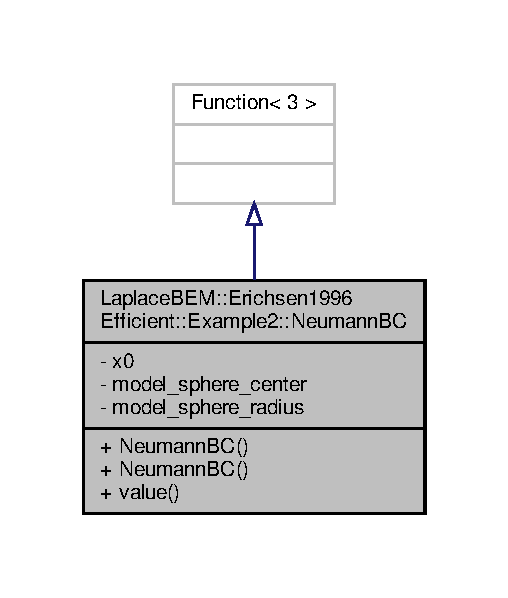
\includegraphics[width=244pt]{classLaplaceBEM_1_1Erichsen1996Efficient_1_1Example2_1_1NeumannBC__inherit__graph}
\end{center}
\end{figure}


Collaboration diagram for Laplace\+B\+EM\+:\+:Erichsen1996\+Efficient\+:\+:Example2\+:\+:Neumann\+BC\+:\nopagebreak
\begin{figure}[H]
\begin{center}
\leavevmode
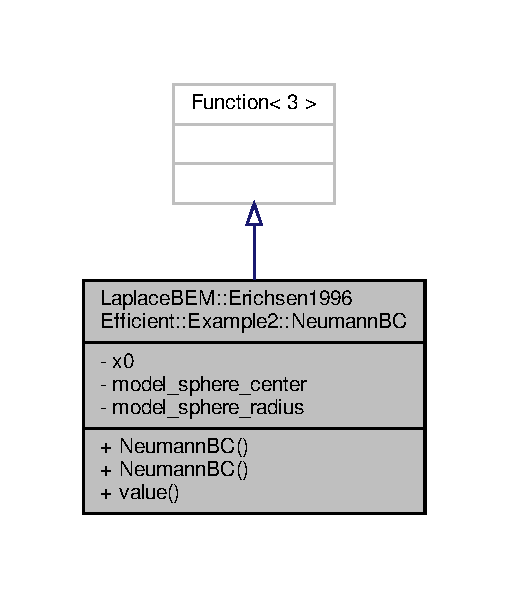
\includegraphics[width=244pt]{classLaplaceBEM_1_1Erichsen1996Efficient_1_1Example2_1_1NeumannBC__coll__graph}
\end{center}
\end{figure}
\subsection*{Public Member Functions}
\begin{DoxyCompactItemize}
\item 
\mbox{\Hypertarget{classLaplaceBEM_1_1Erichsen1996Efficient_1_1Example2_1_1NeumannBC_af03728f3f5a5e09a1d6e36aa0dea1c72}\label{classLaplaceBEM_1_1Erichsen1996Efficient_1_1Example2_1_1NeumannBC_af03728f3f5a5e09a1d6e36aa0dea1c72}} 
{\bfseries Neumann\+BC} (const Point$<$ 3 $>$ \&x0, const Point$<$ 3 $>$ \&center, double radius)
\item 
\mbox{\Hypertarget{classLaplaceBEM_1_1Erichsen1996Efficient_1_1Example2_1_1NeumannBC_aebf1e1dee97d780e504e96b350e88c17}\label{classLaplaceBEM_1_1Erichsen1996Efficient_1_1Example2_1_1NeumannBC_aebf1e1dee97d780e504e96b350e88c17}} 
double {\bfseries value} (const Point$<$ 3 $>$ \&p, const unsigned int component=0) const
\end{DoxyCompactItemize}
\subsection*{Private Attributes}
\begin{DoxyCompactItemize}
\item 
\mbox{\Hypertarget{classLaplaceBEM_1_1Erichsen1996Efficient_1_1Example2_1_1NeumannBC_a3d5d3c953fa5e212eef7acdc0fface73}\label{classLaplaceBEM_1_1Erichsen1996Efficient_1_1Example2_1_1NeumannBC_a3d5d3c953fa5e212eef7acdc0fface73}} 
Point$<$ 3 $>$ {\bfseries x0}
\item 
\mbox{\Hypertarget{classLaplaceBEM_1_1Erichsen1996Efficient_1_1Example2_1_1NeumannBC_a58da53269bae22bf7fe25d5c8bf8add3}\label{classLaplaceBEM_1_1Erichsen1996Efficient_1_1Example2_1_1NeumannBC_a58da53269bae22bf7fe25d5c8bf8add3}} 
Point$<$ 3 $>$ {\bfseries model\+\_\+sphere\+\_\+center}
\item 
\mbox{\Hypertarget{classLaplaceBEM_1_1Erichsen1996Efficient_1_1Example2_1_1NeumannBC_a1d7bec12c397d5b5255f3eba2a0d83c7}\label{classLaplaceBEM_1_1Erichsen1996Efficient_1_1Example2_1_1NeumannBC_a1d7bec12c397d5b5255f3eba2a0d83c7}} 
double {\bfseries model\+\_\+sphere\+\_\+radius}
\end{DoxyCompactItemize}


The documentation for this class was generated from the following file\+:\begin{DoxyCompactItemize}
\item 
/home/jihuan/\+Projects/deal.\+ii/program/dealii-\/9.\+1.\+1/examples/laplace-\/bem/include/erichsen1996efficient\+\_\+example2.\+h\end{DoxyCompactItemize}

\hypertarget{structLaplaceBEM_1_1PairCellWisePerTaskData}{}\section{Laplace\+B\+EM\+:\+:Pair\+Cell\+Wise\+Per\+Task\+Data Struct Reference}
\label{structLaplaceBEM_1_1PairCellWisePerTaskData}\index{Laplace\+B\+E\+M\+::\+Pair\+Cell\+Wise\+Per\+Task\+Data@{Laplace\+B\+E\+M\+::\+Pair\+Cell\+Wise\+Per\+Task\+Data}}


Collaboration diagram for Laplace\+B\+EM\+:\+:Pair\+Cell\+Wise\+Per\+Task\+Data\+:\nopagebreak
\begin{figure}[H]
\begin{center}
\leavevmode
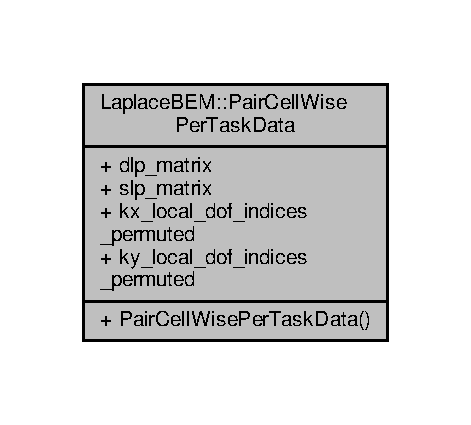
\includegraphics[width=226pt]{structLaplaceBEM_1_1PairCellWisePerTaskData__coll__graph}
\end{center}
\end{figure}
\subsection*{Public Member Functions}
\begin{DoxyCompactItemize}
\item 
\mbox{\Hypertarget{structLaplaceBEM_1_1PairCellWisePerTaskData_ab181d0f788fa5fb1193b5a1559458ce5}\label{structLaplaceBEM_1_1PairCellWisePerTaskData_ab181d0f788fa5fb1193b5a1559458ce5}} 
{\bfseries Pair\+Cell\+Wise\+Per\+Task\+Data} (const Finite\+Element$<$ 2, 3 $>$ \&kx\+\_\+fe, const Finite\+Element$<$ 2, 3 $>$ \&ky\+\_\+fe)
\end{DoxyCompactItemize}
\subsection*{Public Attributes}
\begin{DoxyCompactItemize}
\item 
\mbox{\Hypertarget{structLaplaceBEM_1_1PairCellWisePerTaskData_a35b4a45b92bf0c8c36107fdc80c966cb}\label{structLaplaceBEM_1_1PairCellWisePerTaskData_a35b4a45b92bf0c8c36107fdc80c966cb}} 
Full\+Matrix$<$ double $>$ {\bfseries dlp\+\_\+matrix}
\item 
\mbox{\Hypertarget{structLaplaceBEM_1_1PairCellWisePerTaskData_aa96b7a6991e47201c7f1f6a9fdfa8680}\label{structLaplaceBEM_1_1PairCellWisePerTaskData_aa96b7a6991e47201c7f1f6a9fdfa8680}} 
Full\+Matrix$<$ double $>$ {\bfseries slp\+\_\+matrix}
\item 
\mbox{\Hypertarget{structLaplaceBEM_1_1PairCellWisePerTaskData_ad258060f7c6dfce99a40508320bb54bc}\label{structLaplaceBEM_1_1PairCellWisePerTaskData_ad258060f7c6dfce99a40508320bb54bc}} 
std\+::vector$<$ types\+::global\+\_\+dof\+\_\+index $>$ {\bfseries kx\+\_\+local\+\_\+dof\+\_\+indices\+\_\+permuted}
\item 
\mbox{\Hypertarget{structLaplaceBEM_1_1PairCellWisePerTaskData_a4ebad8073a36303fd26b67acd9a0d9b8}\label{structLaplaceBEM_1_1PairCellWisePerTaskData_a4ebad8073a36303fd26b67acd9a0d9b8}} 
std\+::vector$<$ types\+::global\+\_\+dof\+\_\+index $>$ {\bfseries ky\+\_\+local\+\_\+dof\+\_\+indices\+\_\+permuted}
\end{DoxyCompactItemize}


The documentation for this struct was generated from the following file\+:\begin{DoxyCompactItemize}
\item 
/home/jihuan/\+Projects/deal.\+ii/program/dealii-\/9.\+1.\+1/examples/laplace-\/bem/include/\hyperlink{laplace__bem_8h}{laplace\+\_\+bem.\+h}\end{DoxyCompactItemize}

\hypertarget{structLaplaceBEM_1_1PairCellWiseScratchData}{}\section{Laplace\+B\+EM\+:\+:Pair\+Cell\+Wise\+Scratch\+Data Struct Reference}
\label{structLaplaceBEM_1_1PairCellWiseScratchData}\index{Laplace\+B\+E\+M\+::\+Pair\+Cell\+Wise\+Scratch\+Data@{Laplace\+B\+E\+M\+::\+Pair\+Cell\+Wise\+Scratch\+Data}}


Collaboration diagram for Laplace\+B\+EM\+:\+:Pair\+Cell\+Wise\+Scratch\+Data\+:\nopagebreak
\begin{figure}[H]
\begin{center}
\leavevmode
\includegraphics[height=550pt]{structLaplaceBEM_1_1PairCellWiseScratchData__coll__graph}
\end{center}
\end{figure}
\subsection*{Public Member Functions}
\begin{DoxyCompactItemize}
\item 
\mbox{\Hypertarget{structLaplaceBEM_1_1PairCellWiseScratchData_a728f0084479845ef359dde917ee2927d}\label{structLaplaceBEM_1_1PairCellWiseScratchData_a728f0084479845ef359dde917ee2927d}} 
{\bfseries Pair\+Cell\+Wise\+Scratch\+Data} (const Finite\+Element$<$ 2, 3 $>$ \&kx\+\_\+fe, const Finite\+Element$<$ 2, 3 $>$ \&ky\+\_\+fe, const \hyperlink{classLaplaceBEM_1_1BEMValues}{B\+E\+M\+Values}$<$ 2, 3 $>$ \&bem\+\_\+values)
\end{DoxyCompactItemize}
\subsection*{Public Attributes}
\begin{DoxyCompactItemize}
\item 
std\+::vector$<$ types\+::global\+\_\+dof\+\_\+index $>$ \hyperlink{structLaplaceBEM_1_1PairCellWiseScratchData_a2001013e06428347d301c51380dfe9c8}{vertex\+\_\+dof\+\_\+index\+\_\+intersection}
\item 
std\+::vector$<$ Point$<$ 3 $>$ $>$ \hyperlink{structLaplaceBEM_1_1PairCellWiseScratchData_a3d2f3d03a4c9edd68c5b6e23707a0284}{kx\+\_\+support\+\_\+points\+\_\+hierarchical}
\item 
std\+::vector$<$ Point$<$ 3 $>$ $>$ \hyperlink{structLaplaceBEM_1_1PairCellWiseScratchData_ab87c5e42ccd17d45d97052bda9576dce}{ky\+\_\+support\+\_\+points\+\_\+hierarchical}
\item 
std\+::vector$<$ Point$<$ 3 $>$ $>$ \hyperlink{structLaplaceBEM_1_1PairCellWiseScratchData_a32b2da930b6ad0488446e5b28da7565d}{kx\+\_\+support\+\_\+points\+\_\+permuted}
\item 
std\+::vector$<$ Point$<$ 3 $>$ $>$ \hyperlink{structLaplaceBEM_1_1PairCellWiseScratchData_a998570a30f2cf4069e2e08430b253ead}{ky\+\_\+support\+\_\+points\+\_\+permuted}
\item 
std\+::vector$<$ types\+::global\+\_\+dof\+\_\+index $>$ \hyperlink{structLaplaceBEM_1_1PairCellWiseScratchData_a2f1f9ec98f5c725bef002e01259d95a2}{kx\+\_\+local\+\_\+dof\+\_\+indices\+\_\+hierarchical}
\item 
std\+::vector$<$ types\+::global\+\_\+dof\+\_\+index $>$ \hyperlink{structLaplaceBEM_1_1PairCellWiseScratchData_a04052a9ef0a6f5ab440ffed7c1727e32}{ky\+\_\+local\+\_\+dof\+\_\+indices\+\_\+hierarchical}
\item 
std\+::vector$<$ unsigned int $>$ \hyperlink{structLaplaceBEM_1_1PairCellWiseScratchData_a5292871002dbf2bb4fdf33b255123862}{kx\+\_\+fe\+\_\+poly\+\_\+space\+\_\+numbering\+\_\+inverse}
\item 
std\+::vector$<$ unsigned int $>$ \hyperlink{structLaplaceBEM_1_1PairCellWiseScratchData_a4970716b43febb26cca3705cbcee97ce}{ky\+\_\+fe\+\_\+poly\+\_\+space\+\_\+numbering\+\_\+inverse}
\item 
std\+::vector$<$ unsigned int $>$ \hyperlink{structLaplaceBEM_1_1PairCellWiseScratchData_a444fccb04e87630f9614792070e71238}{ky\+\_\+fe\+\_\+reversed\+\_\+poly\+\_\+space\+\_\+numbering\+\_\+inverse}
\item 
std\+::vector$<$ unsigned int $>$ \hyperlink{structLaplaceBEM_1_1PairCellWiseScratchData_a32bf7e5a46d34fec6116bd2ec75f94c9}{kx\+\_\+local\+\_\+dof\+\_\+permutation}
\item 
std\+::vector$<$ unsigned int $>$ \hyperlink{structLaplaceBEM_1_1PairCellWiseScratchData_a302d0112db325d77a42d1de4018550ec}{ky\+\_\+local\+\_\+dof\+\_\+permutation}
\item 
Table$<$ 2, double $>$ \hyperlink{structLaplaceBEM_1_1PairCellWiseScratchData_afee4ea6d2f9cfb16b2fac08b4453d474}{kx\+\_\+jacobians\+\_\+same\+\_\+panel}
\item 
Table$<$ 2, double $>$ \hyperlink{structLaplaceBEM_1_1PairCellWiseScratchData_ac465e92705daa6b3811d06060aa44ebf}{kx\+\_\+jacobians\+\_\+common\+\_\+edge}
\item 
Table$<$ 2, double $>$ \hyperlink{structLaplaceBEM_1_1PairCellWiseScratchData_a324b41050cc05a58d66142059c221389}{kx\+\_\+jacobians\+\_\+common\+\_\+vertex}
\item 
Table$<$ 2, double $>$ \hyperlink{structLaplaceBEM_1_1PairCellWiseScratchData_a7a26f43e92b8fb0046b20bd6b554da9e}{kx\+\_\+jacobians\+\_\+regular}
\item 
Table$<$ 2, Tensor$<$ 1, 3 $>$ $>$ \hyperlink{structLaplaceBEM_1_1PairCellWiseScratchData_a996a720686a60c1a8e547ae2a416fbd8}{kx\+\_\+normals\+\_\+same\+\_\+panel}
\item 
Table$<$ 2, Tensor$<$ 1, 3 $>$ $>$ \hyperlink{structLaplaceBEM_1_1PairCellWiseScratchData_a281bd24bb9cc4f052e72436287d3020e}{kx\+\_\+normals\+\_\+common\+\_\+edge}
\item 
Table$<$ 2, Tensor$<$ 1, 3 $>$ $>$ \hyperlink{structLaplaceBEM_1_1PairCellWiseScratchData_a9f8757bdb93eb794fa85740c9803de81}{kx\+\_\+normals\+\_\+common\+\_\+vertex}
\item 
Table$<$ 2, Tensor$<$ 1, 3 $>$ $>$ \hyperlink{structLaplaceBEM_1_1PairCellWiseScratchData_a8a9740793ac043e50349fefeb1a0fc0a}{kx\+\_\+normals\+\_\+regular}
\item 
Table$<$ 2, Point$<$ 3 $>$ $>$ \hyperlink{structLaplaceBEM_1_1PairCellWiseScratchData_a96f6236b68431100ea24eaf6bba2da97}{kx\+\_\+quad\+\_\+points\+\_\+same\+\_\+panel}
\item 
Table$<$ 2, Point$<$ 3 $>$ $>$ \hyperlink{structLaplaceBEM_1_1PairCellWiseScratchData_aec980f129e159ccf3038fb2e0389d932}{kx\+\_\+quad\+\_\+points\+\_\+common\+\_\+edge}
\item 
Table$<$ 2, Point$<$ 3 $>$ $>$ \hyperlink{structLaplaceBEM_1_1PairCellWiseScratchData_a395f779ae14e7987e2e2562ec7e80ad7}{kx\+\_\+quad\+\_\+points\+\_\+common\+\_\+vertex}
\item 
Table$<$ 2, Point$<$ 3 $>$ $>$ \hyperlink{structLaplaceBEM_1_1PairCellWiseScratchData_a9aa21e6cae1499b09a2ba49aefea23e0}{kx\+\_\+quad\+\_\+points\+\_\+regular}
\item 
Table$<$ 2, double $>$ \hyperlink{structLaplaceBEM_1_1PairCellWiseScratchData_a914eb8a2b848a3008eea85c35fc012a3}{ky\+\_\+jacobians\+\_\+same\+\_\+panel}
\item 
Table$<$ 2, double $>$ \hyperlink{structLaplaceBEM_1_1PairCellWiseScratchData_aeac246863ee663cd5b977cbb51809542}{ky\+\_\+jacobians\+\_\+common\+\_\+edge}
\item 
Table$<$ 2, double $>$ \hyperlink{structLaplaceBEM_1_1PairCellWiseScratchData_a0a5c02d73cbf27f1c1b8bf4347bc6149}{ky\+\_\+jacobians\+\_\+common\+\_\+vertex}
\item 
Table$<$ 2, double $>$ \hyperlink{structLaplaceBEM_1_1PairCellWiseScratchData_a712bbca9fc35f6953a235cc0950c35d7}{ky\+\_\+jacobians\+\_\+regular}
\item 
Table$<$ 2, Tensor$<$ 1, 3 $>$ $>$ \hyperlink{structLaplaceBEM_1_1PairCellWiseScratchData_ab2ff0498846ca2cb6683f3f16b52b1ed}{ky\+\_\+normals\+\_\+same\+\_\+panel}
\item 
Table$<$ 2, Tensor$<$ 1, 3 $>$ $>$ \hyperlink{structLaplaceBEM_1_1PairCellWiseScratchData_a428bf1cd494daa754755bf8905742fbc}{ky\+\_\+normals\+\_\+common\+\_\+edge}
\item 
Table$<$ 2, Tensor$<$ 1, 3 $>$ $>$ \hyperlink{structLaplaceBEM_1_1PairCellWiseScratchData_aa0c83da483b1ec968e1c9b836d5c684a}{ky\+\_\+normals\+\_\+common\+\_\+vertex}
\item 
Table$<$ 2, Tensor$<$ 1, 3 $>$ $>$ \hyperlink{structLaplaceBEM_1_1PairCellWiseScratchData_ab00760b52f17c91294da7651c21937ee}{ky\+\_\+normals\+\_\+regular}
\item 
Table$<$ 2, Point$<$ 3 $>$ $>$ \hyperlink{structLaplaceBEM_1_1PairCellWiseScratchData_a78dd048ae70be7b101eb670a6c89e75d}{ky\+\_\+quad\+\_\+points\+\_\+same\+\_\+panel}
\item 
Table$<$ 2, Point$<$ 3 $>$ $>$ \hyperlink{structLaplaceBEM_1_1PairCellWiseScratchData_aa777424b41016df40f6d0afce84debab}{ky\+\_\+quad\+\_\+points\+\_\+common\+\_\+edge}
\item 
Table$<$ 2, Point$<$ 3 $>$ $>$ \hyperlink{structLaplaceBEM_1_1PairCellWiseScratchData_acf4cc1caefb3a07b069d0fb67b2891c6}{ky\+\_\+quad\+\_\+points\+\_\+common\+\_\+vertex}
\item 
Table$<$ 2, Point$<$ 3 $>$ $>$ \hyperlink{structLaplaceBEM_1_1PairCellWiseScratchData_abb536bc3bd66be66d8dcd96bc144859e}{ky\+\_\+quad\+\_\+points\+\_\+regular}
\end{DoxyCompactItemize}


\subsection{Member Data Documentation}
\mbox{\Hypertarget{structLaplaceBEM_1_1PairCellWiseScratchData_a5292871002dbf2bb4fdf33b255123862}\label{structLaplaceBEM_1_1PairCellWiseScratchData_a5292871002dbf2bb4fdf33b255123862}} 
\index{Laplace\+B\+E\+M\+::\+Pair\+Cell\+Wise\+Scratch\+Data@{Laplace\+B\+E\+M\+::\+Pair\+Cell\+Wise\+Scratch\+Data}!kx\+\_\+fe\+\_\+poly\+\_\+space\+\_\+numbering\+\_\+inverse@{kx\+\_\+fe\+\_\+poly\+\_\+space\+\_\+numbering\+\_\+inverse}}
\index{kx\+\_\+fe\+\_\+poly\+\_\+space\+\_\+numbering\+\_\+inverse@{kx\+\_\+fe\+\_\+poly\+\_\+space\+\_\+numbering\+\_\+inverse}!Laplace\+B\+E\+M\+::\+Pair\+Cell\+Wise\+Scratch\+Data@{Laplace\+B\+E\+M\+::\+Pair\+Cell\+Wise\+Scratch\+Data}}
\subsubsection{\texorpdfstring{kx\+\_\+fe\+\_\+poly\+\_\+space\+\_\+numbering\+\_\+inverse}{kx\_fe\_poly\_space\_numbering\_inverse}}
{\footnotesize\ttfamily std\+::vector$<$unsigned int$>$ Laplace\+B\+E\+M\+::\+Pair\+Cell\+Wise\+Scratch\+Data\+::kx\+\_\+fe\+\_\+poly\+\_\+space\+\_\+numbering\+\_\+inverse}

The numbering used for accessing the list of Do\+Fs in $K_x$ in the lexicographic order, where the list of Do\+Fs are stored in the hierarchical order. \mbox{\Hypertarget{structLaplaceBEM_1_1PairCellWiseScratchData_ac465e92705daa6b3811d06060aa44ebf}\label{structLaplaceBEM_1_1PairCellWiseScratchData_ac465e92705daa6b3811d06060aa44ebf}} 
\index{Laplace\+B\+E\+M\+::\+Pair\+Cell\+Wise\+Scratch\+Data@{Laplace\+B\+E\+M\+::\+Pair\+Cell\+Wise\+Scratch\+Data}!kx\+\_\+jacobians\+\_\+common\+\_\+edge@{kx\+\_\+jacobians\+\_\+common\+\_\+edge}}
\index{kx\+\_\+jacobians\+\_\+common\+\_\+edge@{kx\+\_\+jacobians\+\_\+common\+\_\+edge}!Laplace\+B\+E\+M\+::\+Pair\+Cell\+Wise\+Scratch\+Data@{Laplace\+B\+E\+M\+::\+Pair\+Cell\+Wise\+Scratch\+Data}}
\subsubsection{\texorpdfstring{kx\+\_\+jacobians\+\_\+common\+\_\+edge}{kx\_jacobians\_common\_edge}}
{\footnotesize\ttfamily Table$<$2, double$>$ Laplace\+B\+E\+M\+::\+Pair\+Cell\+Wise\+Scratch\+Data\+::kx\+\_\+jacobians\+\_\+common\+\_\+edge}

Jacobian from the unit cell to the real cell $K_x$ for each $k_3$ term and at each quadrature point for the common edge case. \mbox{\Hypertarget{structLaplaceBEM_1_1PairCellWiseScratchData_a324b41050cc05a58d66142059c221389}\label{structLaplaceBEM_1_1PairCellWiseScratchData_a324b41050cc05a58d66142059c221389}} 
\index{Laplace\+B\+E\+M\+::\+Pair\+Cell\+Wise\+Scratch\+Data@{Laplace\+B\+E\+M\+::\+Pair\+Cell\+Wise\+Scratch\+Data}!kx\+\_\+jacobians\+\_\+common\+\_\+vertex@{kx\+\_\+jacobians\+\_\+common\+\_\+vertex}}
\index{kx\+\_\+jacobians\+\_\+common\+\_\+vertex@{kx\+\_\+jacobians\+\_\+common\+\_\+vertex}!Laplace\+B\+E\+M\+::\+Pair\+Cell\+Wise\+Scratch\+Data@{Laplace\+B\+E\+M\+::\+Pair\+Cell\+Wise\+Scratch\+Data}}
\subsubsection{\texorpdfstring{kx\+\_\+jacobians\+\_\+common\+\_\+vertex}{kx\_jacobians\_common\_vertex}}
{\footnotesize\ttfamily Table$<$2, double$>$ Laplace\+B\+E\+M\+::\+Pair\+Cell\+Wise\+Scratch\+Data\+::kx\+\_\+jacobians\+\_\+common\+\_\+vertex}

Jacobian from the unit cell to the real cell $K_x$ for each $k_3$ term and at each quadrature point for the common vertex case. \mbox{\Hypertarget{structLaplaceBEM_1_1PairCellWiseScratchData_a7a26f43e92b8fb0046b20bd6b554da9e}\label{structLaplaceBEM_1_1PairCellWiseScratchData_a7a26f43e92b8fb0046b20bd6b554da9e}} 
\index{Laplace\+B\+E\+M\+::\+Pair\+Cell\+Wise\+Scratch\+Data@{Laplace\+B\+E\+M\+::\+Pair\+Cell\+Wise\+Scratch\+Data}!kx\+\_\+jacobians\+\_\+regular@{kx\+\_\+jacobians\+\_\+regular}}
\index{kx\+\_\+jacobians\+\_\+regular@{kx\+\_\+jacobians\+\_\+regular}!Laplace\+B\+E\+M\+::\+Pair\+Cell\+Wise\+Scratch\+Data@{Laplace\+B\+E\+M\+::\+Pair\+Cell\+Wise\+Scratch\+Data}}
\subsubsection{\texorpdfstring{kx\+\_\+jacobians\+\_\+regular}{kx\_jacobians\_regular}}
{\footnotesize\ttfamily Table$<$2, double$>$ Laplace\+B\+E\+M\+::\+Pair\+Cell\+Wise\+Scratch\+Data\+::kx\+\_\+jacobians\+\_\+regular}

Jacobian from the unit cell to the real cell $K_x$ for each $k_3$ term and at each quadrature point for the regular case. \mbox{\Hypertarget{structLaplaceBEM_1_1PairCellWiseScratchData_afee4ea6d2f9cfb16b2fac08b4453d474}\label{structLaplaceBEM_1_1PairCellWiseScratchData_afee4ea6d2f9cfb16b2fac08b4453d474}} 
\index{Laplace\+B\+E\+M\+::\+Pair\+Cell\+Wise\+Scratch\+Data@{Laplace\+B\+E\+M\+::\+Pair\+Cell\+Wise\+Scratch\+Data}!kx\+\_\+jacobians\+\_\+same\+\_\+panel@{kx\+\_\+jacobians\+\_\+same\+\_\+panel}}
\index{kx\+\_\+jacobians\+\_\+same\+\_\+panel@{kx\+\_\+jacobians\+\_\+same\+\_\+panel}!Laplace\+B\+E\+M\+::\+Pair\+Cell\+Wise\+Scratch\+Data@{Laplace\+B\+E\+M\+::\+Pair\+Cell\+Wise\+Scratch\+Data}}
\subsubsection{\texorpdfstring{kx\+\_\+jacobians\+\_\+same\+\_\+panel}{kx\_jacobians\_same\_panel}}
{\footnotesize\ttfamily Table$<$2, double$>$ Laplace\+B\+E\+M\+::\+Pair\+Cell\+Wise\+Scratch\+Data\+::kx\+\_\+jacobians\+\_\+same\+\_\+panel}

Jacobian from the unit cell to the real cell $K_x$ for each $k_3$ term and at each quadrature point for the same panel case. \mbox{\Hypertarget{structLaplaceBEM_1_1PairCellWiseScratchData_a2f1f9ec98f5c725bef002e01259d95a2}\label{structLaplaceBEM_1_1PairCellWiseScratchData_a2f1f9ec98f5c725bef002e01259d95a2}} 
\index{Laplace\+B\+E\+M\+::\+Pair\+Cell\+Wise\+Scratch\+Data@{Laplace\+B\+E\+M\+::\+Pair\+Cell\+Wise\+Scratch\+Data}!kx\+\_\+local\+\_\+dof\+\_\+indices\+\_\+hierarchical@{kx\+\_\+local\+\_\+dof\+\_\+indices\+\_\+hierarchical}}
\index{kx\+\_\+local\+\_\+dof\+\_\+indices\+\_\+hierarchical@{kx\+\_\+local\+\_\+dof\+\_\+indices\+\_\+hierarchical}!Laplace\+B\+E\+M\+::\+Pair\+Cell\+Wise\+Scratch\+Data@{Laplace\+B\+E\+M\+::\+Pair\+Cell\+Wise\+Scratch\+Data}}
\subsubsection{\texorpdfstring{kx\+\_\+local\+\_\+dof\+\_\+indices\+\_\+hierarchical}{kx\_local\_dof\_indices\_hierarchical}}
{\footnotesize\ttfamily std\+::vector$<$types\+::global\+\_\+dof\+\_\+index$>$ Laplace\+B\+E\+M\+::\+Pair\+Cell\+Wise\+Scratch\+Data\+::kx\+\_\+local\+\_\+dof\+\_\+indices\+\_\+hierarchical}

The list of DoF indices in $K_x$ which are ordered in the hierarchical order. This is directly retrieved from the function {\ttfamily Do\+F\+Handler\+::cell\+\_\+iterator\+::get\+\_\+dof\+\_\+indices}. 

Referenced by Laplace\+B\+E\+M\+::\+Erichsen1996\+Efficient\+::\+Example2\+::assemble\+\_\+on\+\_\+one\+\_\+pair\+\_\+of\+\_\+cells().

\mbox{\Hypertarget{structLaplaceBEM_1_1PairCellWiseScratchData_a32bf7e5a46d34fec6116bd2ec75f94c9}\label{structLaplaceBEM_1_1PairCellWiseScratchData_a32bf7e5a46d34fec6116bd2ec75f94c9}} 
\index{Laplace\+B\+E\+M\+::\+Pair\+Cell\+Wise\+Scratch\+Data@{Laplace\+B\+E\+M\+::\+Pair\+Cell\+Wise\+Scratch\+Data}!kx\+\_\+local\+\_\+dof\+\_\+permutation@{kx\+\_\+local\+\_\+dof\+\_\+permutation}}
\index{kx\+\_\+local\+\_\+dof\+\_\+permutation@{kx\+\_\+local\+\_\+dof\+\_\+permutation}!Laplace\+B\+E\+M\+::\+Pair\+Cell\+Wise\+Scratch\+Data@{Laplace\+B\+E\+M\+::\+Pair\+Cell\+Wise\+Scratch\+Data}}
\subsubsection{\texorpdfstring{kx\+\_\+local\+\_\+dof\+\_\+permutation}{kx\_local\_dof\_permutation}}
{\footnotesize\ttfamily std\+::vector$<$unsigned int$>$ Laplace\+B\+E\+M\+::\+Pair\+Cell\+Wise\+Scratch\+Data\+::kx\+\_\+local\+\_\+dof\+\_\+permutation}

The numbering used for accessing the list of support points and associated DoF indices in $K_x$ in the lexicographic order by starting from a specific vertex, where the list of support points and associated DoF indices are stored in the hierarchical order.


\begin{DoxyDescription}
\item[Note ]\char`\"{}\+By starting from a specific vertex\char`\"{} means\+:
\begin{DoxyEnumerate}
\item In the same panel case, this numbering is not used because the first vertex is the starting point by default.
\item In the common edge case, start from the vertex which is the starting point of the common edge.
\item In the common vertex case, start from the common vertex.
\item In the regular panel case, same as the same panel case. 
\end{DoxyEnumerate}
\end{DoxyDescription}\mbox{\Hypertarget{structLaplaceBEM_1_1PairCellWiseScratchData_a281bd24bb9cc4f052e72436287d3020e}\label{structLaplaceBEM_1_1PairCellWiseScratchData_a281bd24bb9cc4f052e72436287d3020e}} 
\index{Laplace\+B\+E\+M\+::\+Pair\+Cell\+Wise\+Scratch\+Data@{Laplace\+B\+E\+M\+::\+Pair\+Cell\+Wise\+Scratch\+Data}!kx\+\_\+normals\+\_\+common\+\_\+edge@{kx\+\_\+normals\+\_\+common\+\_\+edge}}
\index{kx\+\_\+normals\+\_\+common\+\_\+edge@{kx\+\_\+normals\+\_\+common\+\_\+edge}!Laplace\+B\+E\+M\+::\+Pair\+Cell\+Wise\+Scratch\+Data@{Laplace\+B\+E\+M\+::\+Pair\+Cell\+Wise\+Scratch\+Data}}
\subsubsection{\texorpdfstring{kx\+\_\+normals\+\_\+common\+\_\+edge}{kx\_normals\_common\_edge}}
{\footnotesize\ttfamily Table$<$2, Tensor$<$1, 3$>$ $>$ Laplace\+B\+E\+M\+::\+Pair\+Cell\+Wise\+Scratch\+Data\+::kx\+\_\+normals\+\_\+common\+\_\+edge}

Normal vector at each quadrature point in the real cell $K_x$ for the common edge case. \mbox{\Hypertarget{structLaplaceBEM_1_1PairCellWiseScratchData_a9f8757bdb93eb794fa85740c9803de81}\label{structLaplaceBEM_1_1PairCellWiseScratchData_a9f8757bdb93eb794fa85740c9803de81}} 
\index{Laplace\+B\+E\+M\+::\+Pair\+Cell\+Wise\+Scratch\+Data@{Laplace\+B\+E\+M\+::\+Pair\+Cell\+Wise\+Scratch\+Data}!kx\+\_\+normals\+\_\+common\+\_\+vertex@{kx\+\_\+normals\+\_\+common\+\_\+vertex}}
\index{kx\+\_\+normals\+\_\+common\+\_\+vertex@{kx\+\_\+normals\+\_\+common\+\_\+vertex}!Laplace\+B\+E\+M\+::\+Pair\+Cell\+Wise\+Scratch\+Data@{Laplace\+B\+E\+M\+::\+Pair\+Cell\+Wise\+Scratch\+Data}}
\subsubsection{\texorpdfstring{kx\+\_\+normals\+\_\+common\+\_\+vertex}{kx\_normals\_common\_vertex}}
{\footnotesize\ttfamily Table$<$2, Tensor$<$1, 3$>$ $>$ Laplace\+B\+E\+M\+::\+Pair\+Cell\+Wise\+Scratch\+Data\+::kx\+\_\+normals\+\_\+common\+\_\+vertex}

Normal vector at each quadrature point in the real cell $K_x$ for the common vertex case. \mbox{\Hypertarget{structLaplaceBEM_1_1PairCellWiseScratchData_a8a9740793ac043e50349fefeb1a0fc0a}\label{structLaplaceBEM_1_1PairCellWiseScratchData_a8a9740793ac043e50349fefeb1a0fc0a}} 
\index{Laplace\+B\+E\+M\+::\+Pair\+Cell\+Wise\+Scratch\+Data@{Laplace\+B\+E\+M\+::\+Pair\+Cell\+Wise\+Scratch\+Data}!kx\+\_\+normals\+\_\+regular@{kx\+\_\+normals\+\_\+regular}}
\index{kx\+\_\+normals\+\_\+regular@{kx\+\_\+normals\+\_\+regular}!Laplace\+B\+E\+M\+::\+Pair\+Cell\+Wise\+Scratch\+Data@{Laplace\+B\+E\+M\+::\+Pair\+Cell\+Wise\+Scratch\+Data}}
\subsubsection{\texorpdfstring{kx\+\_\+normals\+\_\+regular}{kx\_normals\_regular}}
{\footnotesize\ttfamily Table$<$2, Tensor$<$1, 3$>$ $>$ Laplace\+B\+E\+M\+::\+Pair\+Cell\+Wise\+Scratch\+Data\+::kx\+\_\+normals\+\_\+regular}

Normal vector at each quadrature point in the real cell $K_x$ for the regular case. \mbox{\Hypertarget{structLaplaceBEM_1_1PairCellWiseScratchData_a996a720686a60c1a8e547ae2a416fbd8}\label{structLaplaceBEM_1_1PairCellWiseScratchData_a996a720686a60c1a8e547ae2a416fbd8}} 
\index{Laplace\+B\+E\+M\+::\+Pair\+Cell\+Wise\+Scratch\+Data@{Laplace\+B\+E\+M\+::\+Pair\+Cell\+Wise\+Scratch\+Data}!kx\+\_\+normals\+\_\+same\+\_\+panel@{kx\+\_\+normals\+\_\+same\+\_\+panel}}
\index{kx\+\_\+normals\+\_\+same\+\_\+panel@{kx\+\_\+normals\+\_\+same\+\_\+panel}!Laplace\+B\+E\+M\+::\+Pair\+Cell\+Wise\+Scratch\+Data@{Laplace\+B\+E\+M\+::\+Pair\+Cell\+Wise\+Scratch\+Data}}
\subsubsection{\texorpdfstring{kx\+\_\+normals\+\_\+same\+\_\+panel}{kx\_normals\_same\_panel}}
{\footnotesize\ttfamily Table$<$2, Tensor$<$1, 3$>$ $>$ Laplace\+B\+E\+M\+::\+Pair\+Cell\+Wise\+Scratch\+Data\+::kx\+\_\+normals\+\_\+same\+\_\+panel}

Normal vector at each quadrature point in the real cell $K_x$ for the same panel case. \mbox{\Hypertarget{structLaplaceBEM_1_1PairCellWiseScratchData_aec980f129e159ccf3038fb2e0389d932}\label{structLaplaceBEM_1_1PairCellWiseScratchData_aec980f129e159ccf3038fb2e0389d932}} 
\index{Laplace\+B\+E\+M\+::\+Pair\+Cell\+Wise\+Scratch\+Data@{Laplace\+B\+E\+M\+::\+Pair\+Cell\+Wise\+Scratch\+Data}!kx\+\_\+quad\+\_\+points\+\_\+common\+\_\+edge@{kx\+\_\+quad\+\_\+points\+\_\+common\+\_\+edge}}
\index{kx\+\_\+quad\+\_\+points\+\_\+common\+\_\+edge@{kx\+\_\+quad\+\_\+points\+\_\+common\+\_\+edge}!Laplace\+B\+E\+M\+::\+Pair\+Cell\+Wise\+Scratch\+Data@{Laplace\+B\+E\+M\+::\+Pair\+Cell\+Wise\+Scratch\+Data}}
\subsubsection{\texorpdfstring{kx\+\_\+quad\+\_\+points\+\_\+common\+\_\+edge}{kx\_quad\_points\_common\_edge}}
{\footnotesize\ttfamily Table$<$2, Point$<$3$>$ $>$ Laplace\+B\+E\+M\+::\+Pair\+Cell\+Wise\+Scratch\+Data\+::kx\+\_\+quad\+\_\+points\+\_\+common\+\_\+edge}

Coordinates in the real cell $K_x$ for each $k_3$ term and each quadrature point for the common edge case. \mbox{\Hypertarget{structLaplaceBEM_1_1PairCellWiseScratchData_a395f779ae14e7987e2e2562ec7e80ad7}\label{structLaplaceBEM_1_1PairCellWiseScratchData_a395f779ae14e7987e2e2562ec7e80ad7}} 
\index{Laplace\+B\+E\+M\+::\+Pair\+Cell\+Wise\+Scratch\+Data@{Laplace\+B\+E\+M\+::\+Pair\+Cell\+Wise\+Scratch\+Data}!kx\+\_\+quad\+\_\+points\+\_\+common\+\_\+vertex@{kx\+\_\+quad\+\_\+points\+\_\+common\+\_\+vertex}}
\index{kx\+\_\+quad\+\_\+points\+\_\+common\+\_\+vertex@{kx\+\_\+quad\+\_\+points\+\_\+common\+\_\+vertex}!Laplace\+B\+E\+M\+::\+Pair\+Cell\+Wise\+Scratch\+Data@{Laplace\+B\+E\+M\+::\+Pair\+Cell\+Wise\+Scratch\+Data}}
\subsubsection{\texorpdfstring{kx\+\_\+quad\+\_\+points\+\_\+common\+\_\+vertex}{kx\_quad\_points\_common\_vertex}}
{\footnotesize\ttfamily Table$<$2, Point$<$3$>$ $>$ Laplace\+B\+E\+M\+::\+Pair\+Cell\+Wise\+Scratch\+Data\+::kx\+\_\+quad\+\_\+points\+\_\+common\+\_\+vertex}

Coordinates in the real cell $K_x$ for each $k_3$ term and each quadrature point for the common vertex case. \mbox{\Hypertarget{structLaplaceBEM_1_1PairCellWiseScratchData_a9aa21e6cae1499b09a2ba49aefea23e0}\label{structLaplaceBEM_1_1PairCellWiseScratchData_a9aa21e6cae1499b09a2ba49aefea23e0}} 
\index{Laplace\+B\+E\+M\+::\+Pair\+Cell\+Wise\+Scratch\+Data@{Laplace\+B\+E\+M\+::\+Pair\+Cell\+Wise\+Scratch\+Data}!kx\+\_\+quad\+\_\+points\+\_\+regular@{kx\+\_\+quad\+\_\+points\+\_\+regular}}
\index{kx\+\_\+quad\+\_\+points\+\_\+regular@{kx\+\_\+quad\+\_\+points\+\_\+regular}!Laplace\+B\+E\+M\+::\+Pair\+Cell\+Wise\+Scratch\+Data@{Laplace\+B\+E\+M\+::\+Pair\+Cell\+Wise\+Scratch\+Data}}
\subsubsection{\texorpdfstring{kx\+\_\+quad\+\_\+points\+\_\+regular}{kx\_quad\_points\_regular}}
{\footnotesize\ttfamily Table$<$2, Point$<$3$>$ $>$ Laplace\+B\+E\+M\+::\+Pair\+Cell\+Wise\+Scratch\+Data\+::kx\+\_\+quad\+\_\+points\+\_\+regular}

Coordinates in the real cell $K_x$ for each $k_3$ term and each quadrature point for the regular case. \mbox{\Hypertarget{structLaplaceBEM_1_1PairCellWiseScratchData_a96f6236b68431100ea24eaf6bba2da97}\label{structLaplaceBEM_1_1PairCellWiseScratchData_a96f6236b68431100ea24eaf6bba2da97}} 
\index{Laplace\+B\+E\+M\+::\+Pair\+Cell\+Wise\+Scratch\+Data@{Laplace\+B\+E\+M\+::\+Pair\+Cell\+Wise\+Scratch\+Data}!kx\+\_\+quad\+\_\+points\+\_\+same\+\_\+panel@{kx\+\_\+quad\+\_\+points\+\_\+same\+\_\+panel}}
\index{kx\+\_\+quad\+\_\+points\+\_\+same\+\_\+panel@{kx\+\_\+quad\+\_\+points\+\_\+same\+\_\+panel}!Laplace\+B\+E\+M\+::\+Pair\+Cell\+Wise\+Scratch\+Data@{Laplace\+B\+E\+M\+::\+Pair\+Cell\+Wise\+Scratch\+Data}}
\subsubsection{\texorpdfstring{kx\+\_\+quad\+\_\+points\+\_\+same\+\_\+panel}{kx\_quad\_points\_same\_panel}}
{\footnotesize\ttfamily Table$<$2, Point$<$3$>$ $>$ Laplace\+B\+E\+M\+::\+Pair\+Cell\+Wise\+Scratch\+Data\+::kx\+\_\+quad\+\_\+points\+\_\+same\+\_\+panel}

Coordinates in the real cell $K_x$ for each $k_3$ term and each quadrature point for the same panel case. \mbox{\Hypertarget{structLaplaceBEM_1_1PairCellWiseScratchData_a3d2f3d03a4c9edd68c5b6e23707a0284}\label{structLaplaceBEM_1_1PairCellWiseScratchData_a3d2f3d03a4c9edd68c5b6e23707a0284}} 
\index{Laplace\+B\+E\+M\+::\+Pair\+Cell\+Wise\+Scratch\+Data@{Laplace\+B\+E\+M\+::\+Pair\+Cell\+Wise\+Scratch\+Data}!kx\+\_\+support\+\_\+points\+\_\+hierarchical@{kx\+\_\+support\+\_\+points\+\_\+hierarchical}}
\index{kx\+\_\+support\+\_\+points\+\_\+hierarchical@{kx\+\_\+support\+\_\+points\+\_\+hierarchical}!Laplace\+B\+E\+M\+::\+Pair\+Cell\+Wise\+Scratch\+Data@{Laplace\+B\+E\+M\+::\+Pair\+Cell\+Wise\+Scratch\+Data}}
\subsubsection{\texorpdfstring{kx\+\_\+support\+\_\+points\+\_\+hierarchical}{kx\_support\_points\_hierarchical}}
{\footnotesize\ttfamily std\+::vector$<$Point$<$3$>$ $>$ Laplace\+B\+E\+M\+::\+Pair\+Cell\+Wise\+Scratch\+Data\+::kx\+\_\+support\+\_\+points\+\_\+hierarchical}

List of support points in the real cell $K_x$ in the hierarchical order. 

Referenced by Laplace\+B\+E\+M\+::\+Erichsen1996\+Efficient\+::\+Example2\+::assemble\+\_\+on\+\_\+one\+\_\+pair\+\_\+of\+\_\+cells().

\mbox{\Hypertarget{structLaplaceBEM_1_1PairCellWiseScratchData_a32b2da930b6ad0488446e5b28da7565d}\label{structLaplaceBEM_1_1PairCellWiseScratchData_a32b2da930b6ad0488446e5b28da7565d}} 
\index{Laplace\+B\+E\+M\+::\+Pair\+Cell\+Wise\+Scratch\+Data@{Laplace\+B\+E\+M\+::\+Pair\+Cell\+Wise\+Scratch\+Data}!kx\+\_\+support\+\_\+points\+\_\+permuted@{kx\+\_\+support\+\_\+points\+\_\+permuted}}
\index{kx\+\_\+support\+\_\+points\+\_\+permuted@{kx\+\_\+support\+\_\+points\+\_\+permuted}!Laplace\+B\+E\+M\+::\+Pair\+Cell\+Wise\+Scratch\+Data@{Laplace\+B\+E\+M\+::\+Pair\+Cell\+Wise\+Scratch\+Data}}
\subsubsection{\texorpdfstring{kx\+\_\+support\+\_\+points\+\_\+permuted}{kx\_support\_points\_permuted}}
{\footnotesize\ttfamily std\+::vector$<$Point$<$3$>$ $>$ Laplace\+B\+E\+M\+::\+Pair\+Cell\+Wise\+Scratch\+Data\+::kx\+\_\+support\+\_\+points\+\_\+permuted}

Permuted list of support points in the real cell $K_x$ in the lexicographic order in the same panel case and regular case, and determined by {\ttfamily kx\+\_\+local\+\_\+dof\+\_\+permutation} in the common edge case and common vertex case. \mbox{\Hypertarget{structLaplaceBEM_1_1PairCellWiseScratchData_a4970716b43febb26cca3705cbcee97ce}\label{structLaplaceBEM_1_1PairCellWiseScratchData_a4970716b43febb26cca3705cbcee97ce}} 
\index{Laplace\+B\+E\+M\+::\+Pair\+Cell\+Wise\+Scratch\+Data@{Laplace\+B\+E\+M\+::\+Pair\+Cell\+Wise\+Scratch\+Data}!ky\+\_\+fe\+\_\+poly\+\_\+space\+\_\+numbering\+\_\+inverse@{ky\+\_\+fe\+\_\+poly\+\_\+space\+\_\+numbering\+\_\+inverse}}
\index{ky\+\_\+fe\+\_\+poly\+\_\+space\+\_\+numbering\+\_\+inverse@{ky\+\_\+fe\+\_\+poly\+\_\+space\+\_\+numbering\+\_\+inverse}!Laplace\+B\+E\+M\+::\+Pair\+Cell\+Wise\+Scratch\+Data@{Laplace\+B\+E\+M\+::\+Pair\+Cell\+Wise\+Scratch\+Data}}
\subsubsection{\texorpdfstring{ky\+\_\+fe\+\_\+poly\+\_\+space\+\_\+numbering\+\_\+inverse}{ky\_fe\_poly\_space\_numbering\_inverse}}
{\footnotesize\ttfamily std\+::vector$<$unsigned int$>$ Laplace\+B\+E\+M\+::\+Pair\+Cell\+Wise\+Scratch\+Data\+::ky\+\_\+fe\+\_\+poly\+\_\+space\+\_\+numbering\+\_\+inverse}

The numbering used for accessing the list of Do\+Fs in $K_y$ in the lexicographic order, where the list of Do\+Fs are stored in the hierarchical order. \mbox{\Hypertarget{structLaplaceBEM_1_1PairCellWiseScratchData_a444fccb04e87630f9614792070e71238}\label{structLaplaceBEM_1_1PairCellWiseScratchData_a444fccb04e87630f9614792070e71238}} 
\index{Laplace\+B\+E\+M\+::\+Pair\+Cell\+Wise\+Scratch\+Data@{Laplace\+B\+E\+M\+::\+Pair\+Cell\+Wise\+Scratch\+Data}!ky\+\_\+fe\+\_\+reversed\+\_\+poly\+\_\+space\+\_\+numbering\+\_\+inverse@{ky\+\_\+fe\+\_\+reversed\+\_\+poly\+\_\+space\+\_\+numbering\+\_\+inverse}}
\index{ky\+\_\+fe\+\_\+reversed\+\_\+poly\+\_\+space\+\_\+numbering\+\_\+inverse@{ky\+\_\+fe\+\_\+reversed\+\_\+poly\+\_\+space\+\_\+numbering\+\_\+inverse}!Laplace\+B\+E\+M\+::\+Pair\+Cell\+Wise\+Scratch\+Data@{Laplace\+B\+E\+M\+::\+Pair\+Cell\+Wise\+Scratch\+Data}}
\subsubsection{\texorpdfstring{ky\+\_\+fe\+\_\+reversed\+\_\+poly\+\_\+space\+\_\+numbering\+\_\+inverse}{ky\_fe\_reversed\_poly\_space\_numbering\_inverse}}
{\footnotesize\ttfamily std\+::vector$<$unsigned int$>$ Laplace\+B\+E\+M\+::\+Pair\+Cell\+Wise\+Scratch\+Data\+::ky\+\_\+fe\+\_\+reversed\+\_\+poly\+\_\+space\+\_\+numbering\+\_\+inverse}

The numbering used for accessing the list of Do\+Fs in $K_y$ in the reversed lexicographic order, where the list of Do\+Fs are stored in the hierarchical order.


\begin{DoxyDescription}
\item[Note ]This numbering occurs when $K_x$ and $K_y$ share a common edge. 
\end{DoxyDescription}\mbox{\Hypertarget{structLaplaceBEM_1_1PairCellWiseScratchData_aeac246863ee663cd5b977cbb51809542}\label{structLaplaceBEM_1_1PairCellWiseScratchData_aeac246863ee663cd5b977cbb51809542}} 
\index{Laplace\+B\+E\+M\+::\+Pair\+Cell\+Wise\+Scratch\+Data@{Laplace\+B\+E\+M\+::\+Pair\+Cell\+Wise\+Scratch\+Data}!ky\+\_\+jacobians\+\_\+common\+\_\+edge@{ky\+\_\+jacobians\+\_\+common\+\_\+edge}}
\index{ky\+\_\+jacobians\+\_\+common\+\_\+edge@{ky\+\_\+jacobians\+\_\+common\+\_\+edge}!Laplace\+B\+E\+M\+::\+Pair\+Cell\+Wise\+Scratch\+Data@{Laplace\+B\+E\+M\+::\+Pair\+Cell\+Wise\+Scratch\+Data}}
\subsubsection{\texorpdfstring{ky\+\_\+jacobians\+\_\+common\+\_\+edge}{ky\_jacobians\_common\_edge}}
{\footnotesize\ttfamily Table$<$2, double$>$ Laplace\+B\+E\+M\+::\+Pair\+Cell\+Wise\+Scratch\+Data\+::ky\+\_\+jacobians\+\_\+common\+\_\+edge}

Jacobian from the unit cell to the real cell $K_y$ for each $k_3$ term and at each quadrature point for the common edge case. \mbox{\Hypertarget{structLaplaceBEM_1_1PairCellWiseScratchData_a0a5c02d73cbf27f1c1b8bf4347bc6149}\label{structLaplaceBEM_1_1PairCellWiseScratchData_a0a5c02d73cbf27f1c1b8bf4347bc6149}} 
\index{Laplace\+B\+E\+M\+::\+Pair\+Cell\+Wise\+Scratch\+Data@{Laplace\+B\+E\+M\+::\+Pair\+Cell\+Wise\+Scratch\+Data}!ky\+\_\+jacobians\+\_\+common\+\_\+vertex@{ky\+\_\+jacobians\+\_\+common\+\_\+vertex}}
\index{ky\+\_\+jacobians\+\_\+common\+\_\+vertex@{ky\+\_\+jacobians\+\_\+common\+\_\+vertex}!Laplace\+B\+E\+M\+::\+Pair\+Cell\+Wise\+Scratch\+Data@{Laplace\+B\+E\+M\+::\+Pair\+Cell\+Wise\+Scratch\+Data}}
\subsubsection{\texorpdfstring{ky\+\_\+jacobians\+\_\+common\+\_\+vertex}{ky\_jacobians\_common\_vertex}}
{\footnotesize\ttfamily Table$<$2, double$>$ Laplace\+B\+E\+M\+::\+Pair\+Cell\+Wise\+Scratch\+Data\+::ky\+\_\+jacobians\+\_\+common\+\_\+vertex}

Jacobian from the unit cell to the real cell $K_y$ for each $k_3$ term and at each quadrature point for the common vertex case. \mbox{\Hypertarget{structLaplaceBEM_1_1PairCellWiseScratchData_a712bbca9fc35f6953a235cc0950c35d7}\label{structLaplaceBEM_1_1PairCellWiseScratchData_a712bbca9fc35f6953a235cc0950c35d7}} 
\index{Laplace\+B\+E\+M\+::\+Pair\+Cell\+Wise\+Scratch\+Data@{Laplace\+B\+E\+M\+::\+Pair\+Cell\+Wise\+Scratch\+Data}!ky\+\_\+jacobians\+\_\+regular@{ky\+\_\+jacobians\+\_\+regular}}
\index{ky\+\_\+jacobians\+\_\+regular@{ky\+\_\+jacobians\+\_\+regular}!Laplace\+B\+E\+M\+::\+Pair\+Cell\+Wise\+Scratch\+Data@{Laplace\+B\+E\+M\+::\+Pair\+Cell\+Wise\+Scratch\+Data}}
\subsubsection{\texorpdfstring{ky\+\_\+jacobians\+\_\+regular}{ky\_jacobians\_regular}}
{\footnotesize\ttfamily Table$<$2, double$>$ Laplace\+B\+E\+M\+::\+Pair\+Cell\+Wise\+Scratch\+Data\+::ky\+\_\+jacobians\+\_\+regular}

Jacobian from the unit cell to the real cell $K_y$ for each $k_3$ term and at each quadrature point for the regular case. \mbox{\Hypertarget{structLaplaceBEM_1_1PairCellWiseScratchData_a914eb8a2b848a3008eea85c35fc012a3}\label{structLaplaceBEM_1_1PairCellWiseScratchData_a914eb8a2b848a3008eea85c35fc012a3}} 
\index{Laplace\+B\+E\+M\+::\+Pair\+Cell\+Wise\+Scratch\+Data@{Laplace\+B\+E\+M\+::\+Pair\+Cell\+Wise\+Scratch\+Data}!ky\+\_\+jacobians\+\_\+same\+\_\+panel@{ky\+\_\+jacobians\+\_\+same\+\_\+panel}}
\index{ky\+\_\+jacobians\+\_\+same\+\_\+panel@{ky\+\_\+jacobians\+\_\+same\+\_\+panel}!Laplace\+B\+E\+M\+::\+Pair\+Cell\+Wise\+Scratch\+Data@{Laplace\+B\+E\+M\+::\+Pair\+Cell\+Wise\+Scratch\+Data}}
\subsubsection{\texorpdfstring{ky\+\_\+jacobians\+\_\+same\+\_\+panel}{ky\_jacobians\_same\_panel}}
{\footnotesize\ttfamily Table$<$2, double$>$ Laplace\+B\+E\+M\+::\+Pair\+Cell\+Wise\+Scratch\+Data\+::ky\+\_\+jacobians\+\_\+same\+\_\+panel}

Jacobian from the unit cell to the real cell $K_y$ for each $k_3$ term and at each quadrature point for the same panel case. \mbox{\Hypertarget{structLaplaceBEM_1_1PairCellWiseScratchData_a04052a9ef0a6f5ab440ffed7c1727e32}\label{structLaplaceBEM_1_1PairCellWiseScratchData_a04052a9ef0a6f5ab440ffed7c1727e32}} 
\index{Laplace\+B\+E\+M\+::\+Pair\+Cell\+Wise\+Scratch\+Data@{Laplace\+B\+E\+M\+::\+Pair\+Cell\+Wise\+Scratch\+Data}!ky\+\_\+local\+\_\+dof\+\_\+indices\+\_\+hierarchical@{ky\+\_\+local\+\_\+dof\+\_\+indices\+\_\+hierarchical}}
\index{ky\+\_\+local\+\_\+dof\+\_\+indices\+\_\+hierarchical@{ky\+\_\+local\+\_\+dof\+\_\+indices\+\_\+hierarchical}!Laplace\+B\+E\+M\+::\+Pair\+Cell\+Wise\+Scratch\+Data@{Laplace\+B\+E\+M\+::\+Pair\+Cell\+Wise\+Scratch\+Data}}
\subsubsection{\texorpdfstring{ky\+\_\+local\+\_\+dof\+\_\+indices\+\_\+hierarchical}{ky\_local\_dof\_indices\_hierarchical}}
{\footnotesize\ttfamily std\+::vector$<$types\+::global\+\_\+dof\+\_\+index$>$ Laplace\+B\+E\+M\+::\+Pair\+Cell\+Wise\+Scratch\+Data\+::ky\+\_\+local\+\_\+dof\+\_\+indices\+\_\+hierarchical}

The list of DoF indices in $K_y$ which are ordered in the hierarchical order. This is directly retrieved from the function {\ttfamily Do\+F\+Handler\+::cell\+\_\+iterator\+::get\+\_\+dof\+\_\+indices}. 

Referenced by Laplace\+B\+E\+M\+::\+Erichsen1996\+Efficient\+::\+Example2\+::assemble\+\_\+on\+\_\+one\+\_\+pair\+\_\+of\+\_\+cells().

\mbox{\Hypertarget{structLaplaceBEM_1_1PairCellWiseScratchData_a302d0112db325d77a42d1de4018550ec}\label{structLaplaceBEM_1_1PairCellWiseScratchData_a302d0112db325d77a42d1de4018550ec}} 
\index{Laplace\+B\+E\+M\+::\+Pair\+Cell\+Wise\+Scratch\+Data@{Laplace\+B\+E\+M\+::\+Pair\+Cell\+Wise\+Scratch\+Data}!ky\+\_\+local\+\_\+dof\+\_\+permutation@{ky\+\_\+local\+\_\+dof\+\_\+permutation}}
\index{ky\+\_\+local\+\_\+dof\+\_\+permutation@{ky\+\_\+local\+\_\+dof\+\_\+permutation}!Laplace\+B\+E\+M\+::\+Pair\+Cell\+Wise\+Scratch\+Data@{Laplace\+B\+E\+M\+::\+Pair\+Cell\+Wise\+Scratch\+Data}}
\subsubsection{\texorpdfstring{ky\+\_\+local\+\_\+dof\+\_\+permutation}{ky\_local\_dof\_permutation}}
{\footnotesize\ttfamily std\+::vector$<$unsigned int$>$ Laplace\+B\+E\+M\+::\+Pair\+Cell\+Wise\+Scratch\+Data\+::ky\+\_\+local\+\_\+dof\+\_\+permutation}

The numbering used for accessing the list of support points and associated DoF indices in $K_y$ in the lexicographic order or the reversed lexicographic order by starting from a specific vertex, where the list of support points and associated DoF indices are stored in the hierarchical order.


\begin{DoxyDescription}
\item[Note ]\char`\"{}\+By starting from a specific vertex\char`\"{} means\+:
\begin{DoxyEnumerate}
\item In the same panel case, this numbering is not used because the first vertex is the starting point by default.
\item In the common edge case, start from the vertex which is the starting point of the common edge. And the list of support points and associated DoF indices are accessed in the reversed lexicographic order. Then the cell orientation is reversed and the calculated normal vector should be negated.
\item In the common vertex case, start from the common vertex. And the list of support points and associated DoF indices are accessed in the lexicographic order.
\item In the regular panel case, same as the same panel case. 
\end{DoxyEnumerate}
\end{DoxyDescription}\mbox{\Hypertarget{structLaplaceBEM_1_1PairCellWiseScratchData_a428bf1cd494daa754755bf8905742fbc}\label{structLaplaceBEM_1_1PairCellWiseScratchData_a428bf1cd494daa754755bf8905742fbc}} 
\index{Laplace\+B\+E\+M\+::\+Pair\+Cell\+Wise\+Scratch\+Data@{Laplace\+B\+E\+M\+::\+Pair\+Cell\+Wise\+Scratch\+Data}!ky\+\_\+normals\+\_\+common\+\_\+edge@{ky\+\_\+normals\+\_\+common\+\_\+edge}}
\index{ky\+\_\+normals\+\_\+common\+\_\+edge@{ky\+\_\+normals\+\_\+common\+\_\+edge}!Laplace\+B\+E\+M\+::\+Pair\+Cell\+Wise\+Scratch\+Data@{Laplace\+B\+E\+M\+::\+Pair\+Cell\+Wise\+Scratch\+Data}}
\subsubsection{\texorpdfstring{ky\+\_\+normals\+\_\+common\+\_\+edge}{ky\_normals\_common\_edge}}
{\footnotesize\ttfamily Table$<$2, Tensor$<$1, 3$>$ $>$ Laplace\+B\+E\+M\+::\+Pair\+Cell\+Wise\+Scratch\+Data\+::ky\+\_\+normals\+\_\+common\+\_\+edge}

Normal vector at each quadrature point in the real cell $K_y$ for the common edge case. \mbox{\Hypertarget{structLaplaceBEM_1_1PairCellWiseScratchData_aa0c83da483b1ec968e1c9b836d5c684a}\label{structLaplaceBEM_1_1PairCellWiseScratchData_aa0c83da483b1ec968e1c9b836d5c684a}} 
\index{Laplace\+B\+E\+M\+::\+Pair\+Cell\+Wise\+Scratch\+Data@{Laplace\+B\+E\+M\+::\+Pair\+Cell\+Wise\+Scratch\+Data}!ky\+\_\+normals\+\_\+common\+\_\+vertex@{ky\+\_\+normals\+\_\+common\+\_\+vertex}}
\index{ky\+\_\+normals\+\_\+common\+\_\+vertex@{ky\+\_\+normals\+\_\+common\+\_\+vertex}!Laplace\+B\+E\+M\+::\+Pair\+Cell\+Wise\+Scratch\+Data@{Laplace\+B\+E\+M\+::\+Pair\+Cell\+Wise\+Scratch\+Data}}
\subsubsection{\texorpdfstring{ky\+\_\+normals\+\_\+common\+\_\+vertex}{ky\_normals\_common\_vertex}}
{\footnotesize\ttfamily Table$<$2, Tensor$<$1, 3$>$ $>$ Laplace\+B\+E\+M\+::\+Pair\+Cell\+Wise\+Scratch\+Data\+::ky\+\_\+normals\+\_\+common\+\_\+vertex}

Normal vector at each quadrature point in the real cell $K_y$ for the common vertex case. \mbox{\Hypertarget{structLaplaceBEM_1_1PairCellWiseScratchData_ab00760b52f17c91294da7651c21937ee}\label{structLaplaceBEM_1_1PairCellWiseScratchData_ab00760b52f17c91294da7651c21937ee}} 
\index{Laplace\+B\+E\+M\+::\+Pair\+Cell\+Wise\+Scratch\+Data@{Laplace\+B\+E\+M\+::\+Pair\+Cell\+Wise\+Scratch\+Data}!ky\+\_\+normals\+\_\+regular@{ky\+\_\+normals\+\_\+regular}}
\index{ky\+\_\+normals\+\_\+regular@{ky\+\_\+normals\+\_\+regular}!Laplace\+B\+E\+M\+::\+Pair\+Cell\+Wise\+Scratch\+Data@{Laplace\+B\+E\+M\+::\+Pair\+Cell\+Wise\+Scratch\+Data}}
\subsubsection{\texorpdfstring{ky\+\_\+normals\+\_\+regular}{ky\_normals\_regular}}
{\footnotesize\ttfamily Table$<$2, Tensor$<$1, 3$>$ $>$ Laplace\+B\+E\+M\+::\+Pair\+Cell\+Wise\+Scratch\+Data\+::ky\+\_\+normals\+\_\+regular}

Normal vector at each quadrature point in the real cell $K_y$ for the regular case. \mbox{\Hypertarget{structLaplaceBEM_1_1PairCellWiseScratchData_ab2ff0498846ca2cb6683f3f16b52b1ed}\label{structLaplaceBEM_1_1PairCellWiseScratchData_ab2ff0498846ca2cb6683f3f16b52b1ed}} 
\index{Laplace\+B\+E\+M\+::\+Pair\+Cell\+Wise\+Scratch\+Data@{Laplace\+B\+E\+M\+::\+Pair\+Cell\+Wise\+Scratch\+Data}!ky\+\_\+normals\+\_\+same\+\_\+panel@{ky\+\_\+normals\+\_\+same\+\_\+panel}}
\index{ky\+\_\+normals\+\_\+same\+\_\+panel@{ky\+\_\+normals\+\_\+same\+\_\+panel}!Laplace\+B\+E\+M\+::\+Pair\+Cell\+Wise\+Scratch\+Data@{Laplace\+B\+E\+M\+::\+Pair\+Cell\+Wise\+Scratch\+Data}}
\subsubsection{\texorpdfstring{ky\+\_\+normals\+\_\+same\+\_\+panel}{ky\_normals\_same\_panel}}
{\footnotesize\ttfamily Table$<$2, Tensor$<$1, 3$>$ $>$ Laplace\+B\+E\+M\+::\+Pair\+Cell\+Wise\+Scratch\+Data\+::ky\+\_\+normals\+\_\+same\+\_\+panel}

Normal vector at each quadrature point in the real cell $K_y$ for the same panel case. \mbox{\Hypertarget{structLaplaceBEM_1_1PairCellWiseScratchData_aa777424b41016df40f6d0afce84debab}\label{structLaplaceBEM_1_1PairCellWiseScratchData_aa777424b41016df40f6d0afce84debab}} 
\index{Laplace\+B\+E\+M\+::\+Pair\+Cell\+Wise\+Scratch\+Data@{Laplace\+B\+E\+M\+::\+Pair\+Cell\+Wise\+Scratch\+Data}!ky\+\_\+quad\+\_\+points\+\_\+common\+\_\+edge@{ky\+\_\+quad\+\_\+points\+\_\+common\+\_\+edge}}
\index{ky\+\_\+quad\+\_\+points\+\_\+common\+\_\+edge@{ky\+\_\+quad\+\_\+points\+\_\+common\+\_\+edge}!Laplace\+B\+E\+M\+::\+Pair\+Cell\+Wise\+Scratch\+Data@{Laplace\+B\+E\+M\+::\+Pair\+Cell\+Wise\+Scratch\+Data}}
\subsubsection{\texorpdfstring{ky\+\_\+quad\+\_\+points\+\_\+common\+\_\+edge}{ky\_quad\_points\_common\_edge}}
{\footnotesize\ttfamily Table$<$2, Point$<$3$>$ $>$ Laplace\+B\+E\+M\+::\+Pair\+Cell\+Wise\+Scratch\+Data\+::ky\+\_\+quad\+\_\+points\+\_\+common\+\_\+edge}

Coordinates in the real cell $K_y$ for each $k_3$ term and each quadrature point for the common edge case. \mbox{\Hypertarget{structLaplaceBEM_1_1PairCellWiseScratchData_acf4cc1caefb3a07b069d0fb67b2891c6}\label{structLaplaceBEM_1_1PairCellWiseScratchData_acf4cc1caefb3a07b069d0fb67b2891c6}} 
\index{Laplace\+B\+E\+M\+::\+Pair\+Cell\+Wise\+Scratch\+Data@{Laplace\+B\+E\+M\+::\+Pair\+Cell\+Wise\+Scratch\+Data}!ky\+\_\+quad\+\_\+points\+\_\+common\+\_\+vertex@{ky\+\_\+quad\+\_\+points\+\_\+common\+\_\+vertex}}
\index{ky\+\_\+quad\+\_\+points\+\_\+common\+\_\+vertex@{ky\+\_\+quad\+\_\+points\+\_\+common\+\_\+vertex}!Laplace\+B\+E\+M\+::\+Pair\+Cell\+Wise\+Scratch\+Data@{Laplace\+B\+E\+M\+::\+Pair\+Cell\+Wise\+Scratch\+Data}}
\subsubsection{\texorpdfstring{ky\+\_\+quad\+\_\+points\+\_\+common\+\_\+vertex}{ky\_quad\_points\_common\_vertex}}
{\footnotesize\ttfamily Table$<$2, Point$<$3$>$ $>$ Laplace\+B\+E\+M\+::\+Pair\+Cell\+Wise\+Scratch\+Data\+::ky\+\_\+quad\+\_\+points\+\_\+common\+\_\+vertex}

Coordinates in the real cell $K_y$ for each $k_3$ term and each quadrature point for the common vertex case. \mbox{\Hypertarget{structLaplaceBEM_1_1PairCellWiseScratchData_abb536bc3bd66be66d8dcd96bc144859e}\label{structLaplaceBEM_1_1PairCellWiseScratchData_abb536bc3bd66be66d8dcd96bc144859e}} 
\index{Laplace\+B\+E\+M\+::\+Pair\+Cell\+Wise\+Scratch\+Data@{Laplace\+B\+E\+M\+::\+Pair\+Cell\+Wise\+Scratch\+Data}!ky\+\_\+quad\+\_\+points\+\_\+regular@{ky\+\_\+quad\+\_\+points\+\_\+regular}}
\index{ky\+\_\+quad\+\_\+points\+\_\+regular@{ky\+\_\+quad\+\_\+points\+\_\+regular}!Laplace\+B\+E\+M\+::\+Pair\+Cell\+Wise\+Scratch\+Data@{Laplace\+B\+E\+M\+::\+Pair\+Cell\+Wise\+Scratch\+Data}}
\subsubsection{\texorpdfstring{ky\+\_\+quad\+\_\+points\+\_\+regular}{ky\_quad\_points\_regular}}
{\footnotesize\ttfamily Table$<$2, Point$<$3$>$ $>$ Laplace\+B\+E\+M\+::\+Pair\+Cell\+Wise\+Scratch\+Data\+::ky\+\_\+quad\+\_\+points\+\_\+regular}

Coordinates in the real cell $K_y$ for each $k_3$ term and each quadrature point for the regular case. \mbox{\Hypertarget{structLaplaceBEM_1_1PairCellWiseScratchData_a78dd048ae70be7b101eb670a6c89e75d}\label{structLaplaceBEM_1_1PairCellWiseScratchData_a78dd048ae70be7b101eb670a6c89e75d}} 
\index{Laplace\+B\+E\+M\+::\+Pair\+Cell\+Wise\+Scratch\+Data@{Laplace\+B\+E\+M\+::\+Pair\+Cell\+Wise\+Scratch\+Data}!ky\+\_\+quad\+\_\+points\+\_\+same\+\_\+panel@{ky\+\_\+quad\+\_\+points\+\_\+same\+\_\+panel}}
\index{ky\+\_\+quad\+\_\+points\+\_\+same\+\_\+panel@{ky\+\_\+quad\+\_\+points\+\_\+same\+\_\+panel}!Laplace\+B\+E\+M\+::\+Pair\+Cell\+Wise\+Scratch\+Data@{Laplace\+B\+E\+M\+::\+Pair\+Cell\+Wise\+Scratch\+Data}}
\subsubsection{\texorpdfstring{ky\+\_\+quad\+\_\+points\+\_\+same\+\_\+panel}{ky\_quad\_points\_same\_panel}}
{\footnotesize\ttfamily Table$<$2, Point$<$3$>$ $>$ Laplace\+B\+E\+M\+::\+Pair\+Cell\+Wise\+Scratch\+Data\+::ky\+\_\+quad\+\_\+points\+\_\+same\+\_\+panel}

Coordinates in the real cell $K_y$ for each $k_3$ term and each quadrature point for the same panel case. \mbox{\Hypertarget{structLaplaceBEM_1_1PairCellWiseScratchData_ab87c5e42ccd17d45d97052bda9576dce}\label{structLaplaceBEM_1_1PairCellWiseScratchData_ab87c5e42ccd17d45d97052bda9576dce}} 
\index{Laplace\+B\+E\+M\+::\+Pair\+Cell\+Wise\+Scratch\+Data@{Laplace\+B\+E\+M\+::\+Pair\+Cell\+Wise\+Scratch\+Data}!ky\+\_\+support\+\_\+points\+\_\+hierarchical@{ky\+\_\+support\+\_\+points\+\_\+hierarchical}}
\index{ky\+\_\+support\+\_\+points\+\_\+hierarchical@{ky\+\_\+support\+\_\+points\+\_\+hierarchical}!Laplace\+B\+E\+M\+::\+Pair\+Cell\+Wise\+Scratch\+Data@{Laplace\+B\+E\+M\+::\+Pair\+Cell\+Wise\+Scratch\+Data}}
\subsubsection{\texorpdfstring{ky\+\_\+support\+\_\+points\+\_\+hierarchical}{ky\_support\_points\_hierarchical}}
{\footnotesize\ttfamily std\+::vector$<$Point$<$3$>$ $>$ Laplace\+B\+E\+M\+::\+Pair\+Cell\+Wise\+Scratch\+Data\+::ky\+\_\+support\+\_\+points\+\_\+hierarchical}

List of support points in the real cell $K_y$ in the hierarchical order. 

Referenced by Laplace\+B\+E\+M\+::\+Erichsen1996\+Efficient\+::\+Example2\+::assemble\+\_\+on\+\_\+one\+\_\+pair\+\_\+of\+\_\+cells().

\mbox{\Hypertarget{structLaplaceBEM_1_1PairCellWiseScratchData_a998570a30f2cf4069e2e08430b253ead}\label{structLaplaceBEM_1_1PairCellWiseScratchData_a998570a30f2cf4069e2e08430b253ead}} 
\index{Laplace\+B\+E\+M\+::\+Pair\+Cell\+Wise\+Scratch\+Data@{Laplace\+B\+E\+M\+::\+Pair\+Cell\+Wise\+Scratch\+Data}!ky\+\_\+support\+\_\+points\+\_\+permuted@{ky\+\_\+support\+\_\+points\+\_\+permuted}}
\index{ky\+\_\+support\+\_\+points\+\_\+permuted@{ky\+\_\+support\+\_\+points\+\_\+permuted}!Laplace\+B\+E\+M\+::\+Pair\+Cell\+Wise\+Scratch\+Data@{Laplace\+B\+E\+M\+::\+Pair\+Cell\+Wise\+Scratch\+Data}}
\subsubsection{\texorpdfstring{ky\+\_\+support\+\_\+points\+\_\+permuted}{ky\_support\_points\_permuted}}
{\footnotesize\ttfamily std\+::vector$<$Point$<$3$>$ $>$ Laplace\+B\+E\+M\+::\+Pair\+Cell\+Wise\+Scratch\+Data\+::ky\+\_\+support\+\_\+points\+\_\+permuted}

Permuted list of support points in the real cell $K_y$ in the lexicographic order in the same panel case and regular case, and determined by {\ttfamily ky\+\_\+local\+\_\+dof\+\_\+permutation} in the common edge case and common vertex case. \mbox{\Hypertarget{structLaplaceBEM_1_1PairCellWiseScratchData_a2001013e06428347d301c51380dfe9c8}\label{structLaplaceBEM_1_1PairCellWiseScratchData_a2001013e06428347d301c51380dfe9c8}} 
\index{Laplace\+B\+E\+M\+::\+Pair\+Cell\+Wise\+Scratch\+Data@{Laplace\+B\+E\+M\+::\+Pair\+Cell\+Wise\+Scratch\+Data}!vertex\+\_\+dof\+\_\+index\+\_\+intersection@{vertex\+\_\+dof\+\_\+index\+\_\+intersection}}
\index{vertex\+\_\+dof\+\_\+index\+\_\+intersection@{vertex\+\_\+dof\+\_\+index\+\_\+intersection}!Laplace\+B\+E\+M\+::\+Pair\+Cell\+Wise\+Scratch\+Data@{Laplace\+B\+E\+M\+::\+Pair\+Cell\+Wise\+Scratch\+Data}}
\subsubsection{\texorpdfstring{vertex\+\_\+dof\+\_\+index\+\_\+intersection}{vertex\_dof\_index\_intersection}}
{\footnotesize\ttfamily std\+::vector$<$types\+::global\+\_\+dof\+\_\+index$>$ Laplace\+B\+E\+M\+::\+Pair\+Cell\+Wise\+Scratch\+Data\+::vertex\+\_\+dof\+\_\+index\+\_\+intersection}

The intersection set of the vertex DoF indices for the two cells $K_x$ and $K_y$. 

Referenced by Laplace\+B\+E\+M\+::\+Erichsen1996\+Efficient\+::\+Example2\+::assemble\+\_\+on\+\_\+one\+\_\+pair\+\_\+of\+\_\+cells().



The documentation for this struct was generated from the following file\+:\begin{DoxyCompactItemize}
\item 
/home/jihuan/\+Projects/deal.\+ii/program/dealii-\/9.\+1.\+1/examples/laplace-\/bem/include/\hyperlink{laplace__bem_8h}{laplace\+\_\+bem.\+h}\end{DoxyCompactItemize}

\hypertarget{classRkMatrix}{}\section{Rk\+Matrix$<$ Number $>$ Class Template Reference}
\label{classRkMatrix}\index{Rk\+Matrix$<$ Number $>$@{Rk\+Matrix$<$ Number $>$}}


Collaboration diagram for Rk\+Matrix$<$ Number $>$\+:\nopagebreak
\begin{figure}[H]
\begin{center}
\leavevmode
\includegraphics[height=550pt]{classRkMatrix__coll__graph}
\end{center}
\end{figure}
\subsection*{Public Types}
\begin{DoxyCompactItemize}
\item 
using \hyperlink{classRkMatrix_add060bfc3a4cc77f858c3d6dd58cadd5}{size\+\_\+type} = std\+::make\+\_\+unsigned$<$ types\+::blas\+\_\+int $>$\+::type
\end{DoxyCompactItemize}
\subsection*{Public Member Functions}
\begin{DoxyCompactItemize}
\item 
\hyperlink{classRkMatrix_aa2753ce8e37595824ac275e6b26255cf}{Rk\+Matrix} ()
\item 
\hyperlink{classRkMatrix_a2ed616a9c4e1b12688a903b427260241}{Rk\+Matrix} (const \hyperlink{classRkMatrix_add060bfc3a4cc77f858c3d6dd58cadd5}{size\+\_\+type} \hyperlink{classRkMatrix_a8ca8898bcfedeee135437833f83b144c}{m}, const \hyperlink{classRkMatrix_add060bfc3a4cc77f858c3d6dd58cadd5}{size\+\_\+type} \hyperlink{classRkMatrix_a06d3b6636bb423c391c66e4ccc722687}{n}, const \hyperlink{classRkMatrix_add060bfc3a4cc77f858c3d6dd58cadd5}{size\+\_\+type} fixed\+\_\+rank\+\_\+k)
\item 
\hyperlink{classRkMatrix_a6078a6d21d37f140ff8774b8310a19eb}{Rk\+Matrix} (const \hyperlink{classRkMatrix_add060bfc3a4cc77f858c3d6dd58cadd5}{size\+\_\+type} fixed\+\_\+rank\+\_\+k, \hyperlink{classLAPACKFullMatrixExt}{L\+A\+P\+A\+C\+K\+Full\+Matrix\+Ext}$<$ Number $>$ \&M)
\item 
\hyperlink{classRkMatrix_a08ab45361d9e3cca139727dca31f9bfa}{Rk\+Matrix} (\hyperlink{classLAPACKFullMatrixExt}{L\+A\+P\+A\+C\+K\+Full\+Matrix\+Ext}$<$ Number $>$ \&M)
\item 
\hyperlink{classRkMatrix_acdd046caab506cd04e09b65bb3ffc1f9}{Rk\+Matrix} (const std\+::vector$<$ types\+::global\+\_\+dof\+\_\+index $>$ \&tau, const std\+::vector$<$ types\+::global\+\_\+dof\+\_\+index $>$ \&sigma, const \hyperlink{classRkMatrix_add060bfc3a4cc77f858c3d6dd58cadd5}{size\+\_\+type} fixed\+\_\+rank\+\_\+k, const \hyperlink{classLAPACKFullMatrixExt}{L\+A\+P\+A\+C\+K\+Full\+Matrix\+Ext}$<$ Number $>$ \&M)
\item 
\hyperlink{classRkMatrix_a4cfccf769e03141b5221c1356bd718a1}{Rk\+Matrix} (const std\+::vector$<$ types\+::global\+\_\+dof\+\_\+index $>$ \&tau, const std\+::vector$<$ types\+::global\+\_\+dof\+\_\+index $>$ \&sigma, const \hyperlink{classLAPACKFullMatrixExt}{L\+A\+P\+A\+C\+K\+Full\+Matrix\+Ext}$<$ Number $>$ \&M)
\item 
\hyperlink{classRkMatrix_adf204b7ad92834e63c7f63f6b9ca59a9}{Rk\+Matrix} (const std\+::vector$<$ types\+::global\+\_\+dof\+\_\+index $>$ \&tau, const std\+::vector$<$ types\+::global\+\_\+dof\+\_\+index $>$ \&sigma, const \hyperlink{classRkMatrix_add060bfc3a4cc77f858c3d6dd58cadd5}{size\+\_\+type} fixed\+\_\+rank\+\_\+k, const \hyperlink{classLAPACKFullMatrixExt}{L\+A\+P\+A\+C\+K\+Full\+Matrix\+Ext}$<$ Number $>$ \&M, const std\+::map$<$ types\+::global\+\_\+dof\+\_\+index, size\+\_\+t $>$ \&row\+\_\+index\+\_\+global\+\_\+to\+\_\+local\+\_\+map\+\_\+for\+\_\+M, const std\+::map$<$ types\+::global\+\_\+dof\+\_\+index, size\+\_\+t $>$ \&col\+\_\+index\+\_\+global\+\_\+to\+\_\+local\+\_\+map\+\_\+for\+\_\+M)
\item 
\hyperlink{classRkMatrix_aee16f709a7a73d022add2f044cdcb26a}{Rk\+Matrix} (const std\+::vector$<$ types\+::global\+\_\+dof\+\_\+index $>$ \&tau, const std\+::vector$<$ types\+::global\+\_\+dof\+\_\+index $>$ \&sigma, const \hyperlink{classLAPACKFullMatrixExt}{L\+A\+P\+A\+C\+K\+Full\+Matrix\+Ext}$<$ Number $>$ \&M, const std\+::map$<$ types\+::global\+\_\+dof\+\_\+index, size\+\_\+t $>$ \&row\+\_\+index\+\_\+global\+\_\+to\+\_\+local\+\_\+map\+\_\+for\+\_\+M, const std\+::map$<$ types\+::global\+\_\+dof\+\_\+index, size\+\_\+t $>$ \&col\+\_\+index\+\_\+global\+\_\+to\+\_\+local\+\_\+map\+\_\+for\+\_\+M)
\item 
\hyperlink{classRkMatrix_aa5aff0d31115d7a67ef2f11db0b4ea24}{Rk\+Matrix} (const std\+::vector$<$ types\+::global\+\_\+dof\+\_\+index $>$ \&tau, const std\+::vector$<$ types\+::global\+\_\+dof\+\_\+index $>$ \&sigma, const \hyperlink{classRkMatrix_add060bfc3a4cc77f858c3d6dd58cadd5}{size\+\_\+type} fixed\+\_\+rank\+\_\+k, const \hyperlink{classRkMatrix}{Rk\+Matrix}$<$ Number $>$ \&M)
\item 
\hyperlink{classRkMatrix_a311b3ac28f647cb191eeb97a0b9d5815}{Rk\+Matrix} (const std\+::vector$<$ types\+::global\+\_\+dof\+\_\+index $>$ \&tau, const std\+::vector$<$ types\+::global\+\_\+dof\+\_\+index $>$ \&sigma, const \hyperlink{classRkMatrix}{Rk\+Matrix}$<$ Number $>$ \&M)
\item 
\hyperlink{classRkMatrix_a5a2841fc6a697007fafcab2619fc5390}{Rk\+Matrix} (const std\+::vector$<$ types\+::global\+\_\+dof\+\_\+index $>$ \&tau, const std\+::vector$<$ types\+::global\+\_\+dof\+\_\+index $>$ \&sigma, const \hyperlink{classRkMatrix_add060bfc3a4cc77f858c3d6dd58cadd5}{size\+\_\+type} fixed\+\_\+rank\+\_\+k, const \hyperlink{classRkMatrix}{Rk\+Matrix}$<$ Number $>$ \&M, const std\+::map$<$ types\+::global\+\_\+dof\+\_\+index, size\+\_\+t $>$ \&row\+\_\+index\+\_\+global\+\_\+to\+\_\+local\+\_\+map\+\_\+for\+\_\+M, const std\+::map$<$ types\+::global\+\_\+dof\+\_\+index, size\+\_\+t $>$ \&col\+\_\+index\+\_\+global\+\_\+to\+\_\+local\+\_\+map\+\_\+for\+\_\+M)
\item 
\hyperlink{classRkMatrix_a89ad98e45e6ae6c23a6ffc478c7ebb9f}{Rk\+Matrix} (const std\+::vector$<$ types\+::global\+\_\+dof\+\_\+index $>$ \&tau, const std\+::vector$<$ types\+::global\+\_\+dof\+\_\+index $>$ \&sigma, const \hyperlink{classRkMatrix}{Rk\+Matrix}$<$ Number $>$ \&M, const std\+::map$<$ types\+::global\+\_\+dof\+\_\+index, size\+\_\+t $>$ \&row\+\_\+index\+\_\+global\+\_\+to\+\_\+local\+\_\+map\+\_\+for\+\_\+M, const std\+::map$<$ types\+::global\+\_\+dof\+\_\+index, size\+\_\+t $>$ \&col\+\_\+index\+\_\+global\+\_\+to\+\_\+local\+\_\+map\+\_\+for\+\_\+M)
\item 
\hyperlink{classRkMatrix_a22cbf825bdbff58434ab3d4a6c478b96}{Rk\+Matrix} (const \hyperlink{classLAPACKFullMatrixExt}{L\+A\+P\+A\+C\+K\+Full\+Matrix\+Ext}$<$ Number $>$ \&A, const \hyperlink{classLAPACKFullMatrixExt}{L\+A\+P\+A\+C\+K\+Full\+Matrix\+Ext}$<$ Number $>$ \&B)
\item 
\hyperlink{classRkMatrix_ae15a15d55d04dd677a8dc90dbf789674}{Rk\+Matrix} (const \hyperlink{classRkMatrix_add060bfc3a4cc77f858c3d6dd58cadd5}{size\+\_\+type} fixed\+\_\+rank\+\_\+k, const \hyperlink{classRkMatrix}{Rk\+Matrix}$<$ Number $>$ \&M1, const \hyperlink{classRkMatrix}{Rk\+Matrix}$<$ Number $>$ \&M2, bool is\+\_\+horizontal\+\_\+split)
\item 
\hyperlink{classRkMatrix_a0ef50f2d8d07bcbffa0a6d015dc0d1a4}{Rk\+Matrix} (const \hyperlink{classRkMatrix_add060bfc3a4cc77f858c3d6dd58cadd5}{size\+\_\+type} fixed\+\_\+rank\+\_\+k, const std\+::map$<$ types\+::global\+\_\+dof\+\_\+index, size\+\_\+t $>$ \&row\+\_\+index\+\_\+global\+\_\+to\+\_\+local\+\_\+map\+\_\+for\+\_\+M, const std\+::map$<$ types\+::global\+\_\+dof\+\_\+index, size\+\_\+t $>$ \&col\+\_\+index\+\_\+global\+\_\+to\+\_\+local\+\_\+map\+\_\+for\+\_\+M, const \hyperlink{classRkMatrix}{Rk\+Matrix}$<$ Number $>$ \&M1, const std\+::vector$<$ types\+::global\+\_\+dof\+\_\+index $>$ \&M1\+\_\+tau\+\_\+index\+\_\+set, const std\+::vector$<$ types\+::global\+\_\+dof\+\_\+index $>$ \&M1\+\_\+sigma\+\_\+index\+\_\+set, const \hyperlink{classRkMatrix}{Rk\+Matrix}$<$ Number $>$ \&M2, const std\+::vector$<$ types\+::global\+\_\+dof\+\_\+index $>$ \&M2\+\_\+tau\+\_\+index\+\_\+set, const std\+::vector$<$ types\+::global\+\_\+dof\+\_\+index $>$ \&M2\+\_\+sigma\+\_\+index\+\_\+set, bool is\+\_\+horizontal\+\_\+split)
\item 
\hyperlink{classRkMatrix_ab2826404ecbffa257d56feac015a4c5f}{Rk\+Matrix} (const \hyperlink{classRkMatrix_add060bfc3a4cc77f858c3d6dd58cadd5}{size\+\_\+type} fixed\+\_\+rank\+\_\+k, const \hyperlink{classRkMatrix}{Rk\+Matrix}$<$ Number $>$ \&M11, const \hyperlink{classRkMatrix}{Rk\+Matrix}$<$ Number $>$ \&M12, const \hyperlink{classRkMatrix}{Rk\+Matrix}$<$ Number $>$ \&M21, const \hyperlink{classRkMatrix}{Rk\+Matrix}$<$ Number $>$ \&M22, const Number rank\+\_\+factor=1.\+0)
\item 
\hyperlink{classRkMatrix_a00a2465dfb9445dca842f19fc757d008}{Rk\+Matrix} (const \hyperlink{classRkMatrix_add060bfc3a4cc77f858c3d6dd58cadd5}{size\+\_\+type} fixed\+\_\+rank\+\_\+k, const std\+::map$<$ types\+::global\+\_\+dof\+\_\+index, size\+\_\+t $>$ \&row\+\_\+index\+\_\+global\+\_\+to\+\_\+local\+\_\+map\+\_\+for\+\_\+M, const std\+::map$<$ types\+::global\+\_\+dof\+\_\+index, size\+\_\+t $>$ \&col\+\_\+index\+\_\+global\+\_\+to\+\_\+local\+\_\+map\+\_\+for\+\_\+M, const \hyperlink{classRkMatrix}{Rk\+Matrix}$<$ Number $>$ \&M11, const std\+::vector$<$ types\+::global\+\_\+dof\+\_\+index $>$ \&M11\+\_\+tau\+\_\+index\+\_\+set, const std\+::vector$<$ types\+::global\+\_\+dof\+\_\+index $>$ \&M11\+\_\+sigma\+\_\+index\+\_\+set, const \hyperlink{classRkMatrix}{Rk\+Matrix}$<$ Number $>$ \&M12, const std\+::vector$<$ types\+::global\+\_\+dof\+\_\+index $>$ \&M12\+\_\+tau\+\_\+index\+\_\+set, const std\+::vector$<$ types\+::global\+\_\+dof\+\_\+index $>$ \&M12\+\_\+sigma\+\_\+index\+\_\+set, const \hyperlink{classRkMatrix}{Rk\+Matrix}$<$ Number $>$ \&M21, const std\+::vector$<$ types\+::global\+\_\+dof\+\_\+index $>$ \&M21\+\_\+tau\+\_\+index\+\_\+set, const std\+::vector$<$ types\+::global\+\_\+dof\+\_\+index $>$ \&M21\+\_\+sigma\+\_\+index\+\_\+set, const \hyperlink{classRkMatrix}{Rk\+Matrix}$<$ Number $>$ \&M22, const std\+::vector$<$ types\+::global\+\_\+dof\+\_\+index $>$ \&M22\+\_\+tau\+\_\+index\+\_\+set, const std\+::vector$<$ types\+::global\+\_\+dof\+\_\+index $>$ \&M22\+\_\+sigma\+\_\+index\+\_\+set, const Number rank\+\_\+factor=1.\+0)
\item 
\hyperlink{classRkMatrix_a5f886128ba604cc85f99e3c9c9a07e7c}{Rk\+Matrix} (const \hyperlink{classRkMatrix}{Rk\+Matrix}$<$ Number $>$ \&matrix)
\item 
\hyperlink{classRkMatrix}{Rk\+Matrix}$<$ Number $>$ \& \hyperlink{classRkMatrix_a8894542d0a6cda34a78cccf34eb3f990}{operator=} (const \hyperlink{classRkMatrix}{Rk\+Matrix}$<$ Number $>$ \&matrix)
\item 
void \hyperlink{classRkMatrix_a5457372194e8009bffc7b88f11b95d03}{reinit} (const \hyperlink{classRkMatrix_add060bfc3a4cc77f858c3d6dd58cadd5}{size\+\_\+type} \hyperlink{classRkMatrix_a8ca8898bcfedeee135437833f83b144c}{m}, const \hyperlink{classRkMatrix_add060bfc3a4cc77f858c3d6dd58cadd5}{size\+\_\+type} \hyperlink{classRkMatrix_a06d3b6636bb423c391c66e4ccc722687}{n}, const \hyperlink{classRkMatrix_add060bfc3a4cc77f858c3d6dd58cadd5}{size\+\_\+type} fixed\+\_\+rank\+\_\+k)
\item 
\hyperlink{classRkMatrix_add060bfc3a4cc77f858c3d6dd58cadd5}{size\+\_\+type} \hyperlink{classRkMatrix_a58686c65ca8c952558eae4fa185e7d6a}{get\+\_\+m} () const
\item 
\hyperlink{classRkMatrix_add060bfc3a4cc77f858c3d6dd58cadd5}{size\+\_\+type} \hyperlink{classRkMatrix_a4f719c760482c2ab75cc5647277a9cdd}{get\+\_\+n} () const
\item 
\hyperlink{classRkMatrix_add060bfc3a4cc77f858c3d6dd58cadd5}{size\+\_\+type} \hyperlink{classRkMatrix_a1b2231c1e02862c91f4451e2b0a5fab4}{get\+\_\+rank} () const
\item 
\hyperlink{classRkMatrix_add060bfc3a4cc77f858c3d6dd58cadd5}{size\+\_\+type} \hyperlink{classRkMatrix_ae69122e3ee1c49a4fbe48cf3d7a20581}{get\+\_\+formal\+\_\+rank} () const
\item 
\hyperlink{classLAPACKFullMatrixExt}{L\+A\+P\+A\+C\+K\+Full\+Matrix\+Ext}$<$ Number $>$ \& \hyperlink{classRkMatrix_accfea435fd26c622e491bee475ae788c}{get\+\_\+A} ()
\item 
const \hyperlink{classLAPACKFullMatrixExt}{L\+A\+P\+A\+C\+K\+Full\+Matrix\+Ext}$<$ Number $>$ \& \hyperlink{classRkMatrix_a95e786794895f1ceae2e0f2880e105b3}{get\+\_\+A} () const
\item 
\hyperlink{classLAPACKFullMatrixExt}{L\+A\+P\+A\+C\+K\+Full\+Matrix\+Ext}$<$ Number $>$ \& \hyperlink{classRkMatrix_aca855d29d0dd3036ba75d0e3ca75d88e}{get\+\_\+B} ()
\item 
const \hyperlink{classLAPACKFullMatrixExt}{L\+A\+P\+A\+C\+K\+Full\+Matrix\+Ext}$<$ Number $>$ \& \hyperlink{classRkMatrix_a69695b04d890d753bd3343e4665ca0ba}{get\+\_\+B} () const
\item 
void \hyperlink{classRkMatrix_a384cdf3033d98f90b80d373add20b556}{convert\+To\+Full\+Matrix} (\hyperlink{classLAPACKFullMatrixExt}{L\+A\+P\+A\+C\+K\+Full\+Matrix\+Ext}$<$ Number $>$ \&matrix) const
\item 
void \hyperlink{classRkMatrix_a5305306386e47bcded819ce8d7f7935c}{restrict\+To\+Full\+Matrix} (const std\+::vector$<$ types\+::global\+\_\+dof\+\_\+index $>$ \&tau, const std\+::vector$<$ types\+::global\+\_\+dof\+\_\+index $>$ \&sigma, \hyperlink{classLAPACKFullMatrixExt}{L\+A\+P\+A\+C\+K\+Full\+Matrix\+Ext}$<$ Number $>$ \&matrix) const
\item 
void \hyperlink{classRkMatrix_a0c529b22a8a38c4046a93c4a16ad39ca}{restrict\+To\+Full\+Matrix} (const std\+::vector$<$ types\+::global\+\_\+dof\+\_\+index $>$ \&tau, const std\+::vector$<$ types\+::global\+\_\+dof\+\_\+index $>$ \&sigma, const std\+::map$<$ types\+::global\+\_\+dof\+\_\+index, size\+\_\+t $>$ \&row\+\_\+index\+\_\+global\+\_\+to\+\_\+local\+\_\+map\+\_\+for\+\_\+rk, const std\+::map$<$ types\+::global\+\_\+dof\+\_\+index, size\+\_\+t $>$ \&col\+\_\+index\+\_\+global\+\_\+to\+\_\+local\+\_\+map\+\_\+for\+\_\+rk, \hyperlink{classLAPACKFullMatrixExt}{L\+A\+P\+A\+C\+K\+Full\+Matrix\+Ext}$<$ Number $>$ \&matrix) const
\item 
void \hyperlink{classRkMatrix_aeccb86734649be94a64d76cb613eea79}{print\+\_\+formatted} (std\+::ostream \&out, const unsigned int precision=3, const bool scientific=true, const unsigned int width=0, const char $\ast$zero\+\_\+string=\char`\"{}0\char`\"{}, const double denominator=1., const double threshold=0.) const
\item 
void \hyperlink{classRkMatrix_ada4d32bb08cce5d5e41ee4673bc88e00}{print\+\_\+formatted\+\_\+to\+\_\+mat} (std\+::ostream \&out, const std\+::string \&name, const unsigned int precision=8, const bool scientific=true, const unsigned int width=0, const char $\ast$zero\+\_\+string=\char`\"{}0\char`\"{}, const double denominator=1., const double threshold=0.) const
\item 
void \hyperlink{classRkMatrix_a555e0c3184b8411db1350c8fe1e875a0}{truncate\+\_\+to\+\_\+rank} (\hyperlink{classRkMatrix_add060bfc3a4cc77f858c3d6dd58cadd5}{size\+\_\+type} new\+\_\+rank)
\item 
void \hyperlink{classRkMatrix_a25753b7f6d82dca931992cd975165972}{vmult} (Vector$<$ Number $>$ \&y, const Vector$<$ Number $>$ \&x, const bool adding=false) const
\item 
void \hyperlink{classRkMatrix_a7162dd0c4580dbb5e98715d9b8dd56c1}{Tvmult} (Vector$<$ Number $>$ \&y, const Vector$<$ Number $>$ \&x, const bool adding=false) const
\item 
void \hyperlink{classRkMatrix_a260584004c862292b4ae401cff236588}{add} (\hyperlink{classRkMatrix}{Rk\+Matrix}$<$ Number $>$ \&M, const \hyperlink{classRkMatrix}{Rk\+Matrix}$<$ Number $>$ \&M2) const
\item 
void \hyperlink{classRkMatrix_a99413509ad44b1529f20cb018ce0fc70}{add} (\hyperlink{classRkMatrix}{Rk\+Matrix}$<$ Number $>$ \&M, const Number m2, const \hyperlink{classRkMatrix}{Rk\+Matrix}$<$ Number $>$ \&M2) const
\item 
void \hyperlink{classRkMatrix_a8793188eb93def0030ae90e8f5898813}{add} (const \hyperlink{classRkMatrix}{Rk\+Matrix}$<$ Number $>$ \&M1)
\item 
void \hyperlink{classRkMatrix_a93b434797b9142a4dce0c6a64ba1e89c}{add} (const Number m1, const \hyperlink{classRkMatrix}{Rk\+Matrix}$<$ Number $>$ \&M1)
\item 
void \hyperlink{classRkMatrix_ad8668d42978011b3e65d0381bfb068d5}{add} (\hyperlink{classRkMatrix}{Rk\+Matrix}$<$ Number $>$ \&M, const \hyperlink{classRkMatrix}{Rk\+Matrix}$<$ Number $>$ \&M2, const \hyperlink{classRkMatrix_add060bfc3a4cc77f858c3d6dd58cadd5}{size\+\_\+type} fixed\+\_\+rank\+\_\+k) const
\item 
void \hyperlink{classRkMatrix_aeba05e73aa670b1029c1720e56d10e81}{add} (\hyperlink{classRkMatrix}{Rk\+Matrix}$<$ Number $>$ \&M, const Number m2, const \hyperlink{classRkMatrix}{Rk\+Matrix}$<$ Number $>$ \&M2, const \hyperlink{classRkMatrix_add060bfc3a4cc77f858c3d6dd58cadd5}{size\+\_\+type} fixed\+\_\+rank\+\_\+k) const
\item 
void \hyperlink{classRkMatrix_a1f51eac54ddb43c0670a72da62bc1e55}{add} (const \hyperlink{classRkMatrix}{Rk\+Matrix}$<$ Number $>$ \&M1, const \hyperlink{classRkMatrix_add060bfc3a4cc77f858c3d6dd58cadd5}{size\+\_\+type} fixed\+\_\+rank\+\_\+k)
\item 
void \hyperlink{classRkMatrix_adb27c4eacf80d4e94c20ff96eaf5564d}{add} (const Number m1, const \hyperlink{classRkMatrix}{Rk\+Matrix}$<$ Number $>$ \&M1, const \hyperlink{classRkMatrix_add060bfc3a4cc77f858c3d6dd58cadd5}{size\+\_\+type} fixed\+\_\+rank\+\_\+k)
\item 
void \hyperlink{classRkMatrix_a9ff620f9f71181c794e129d71d76da7c}{assemble\+\_\+from\+\_\+rkmatrix} (const std\+::map$<$ types\+::global\+\_\+dof\+\_\+index, size\+\_\+t $>$ \&row\+\_\+index\+\_\+global\+\_\+to\+\_\+local\+\_\+map, const std\+::map$<$ types\+::global\+\_\+dof\+\_\+index, size\+\_\+t $>$ \&col\+\_\+index\+\_\+global\+\_\+to\+\_\+local\+\_\+map, const \hyperlink{classRkMatrix}{Rk\+Matrix}$<$ Number $>$ \&M, const std\+::vector$<$ types\+::global\+\_\+dof\+\_\+index $>$ \&M\+\_\+tau\+\_\+index\+\_\+set, const std\+::vector$<$ types\+::global\+\_\+dof\+\_\+index $>$ \&M\+\_\+sigma\+\_\+index\+\_\+set, const \hyperlink{classRkMatrix_add060bfc3a4cc77f858c3d6dd58cadd5}{size\+\_\+type} fixed\+\_\+rank\+\_\+k)
\end{DoxyCompactItemize}
\subsection*{Private Attributes}
\begin{DoxyCompactItemize}
\item 
\mbox{\Hypertarget{classRkMatrix_a7bad017da4b56bfe703ac9086fd97d99}\label{classRkMatrix_a7bad017da4b56bfe703ac9086fd97d99}} 
\hyperlink{classLAPACKFullMatrixExt}{L\+A\+P\+A\+C\+K\+Full\+Matrix\+Ext}$<$ Number $>$ {\bfseries A}
\item 
\mbox{\Hypertarget{classRkMatrix_a04f480fcd16ab9918271c7ba199df523}\label{classRkMatrix_a04f480fcd16ab9918271c7ba199df523}} 
\hyperlink{classLAPACKFullMatrixExt}{L\+A\+P\+A\+C\+K\+Full\+Matrix\+Ext}$<$ Number $>$ {\bfseries B}
\item 
\hyperlink{classRkMatrix_add060bfc3a4cc77f858c3d6dd58cadd5}{size\+\_\+type} \hyperlink{classRkMatrix_aa9e60bb24bbe3ab1750f970f296d8256}{rank}
\item 
\hyperlink{classRkMatrix_add060bfc3a4cc77f858c3d6dd58cadd5}{size\+\_\+type} \hyperlink{classRkMatrix_a7e4a8f0500daba627665c6a5ed8888d9}{formal\+\_\+rank}
\item 
\hyperlink{classRkMatrix_add060bfc3a4cc77f858c3d6dd58cadd5}{size\+\_\+type} \hyperlink{classRkMatrix_a8ca8898bcfedeee135437833f83b144c}{m}
\item 
\hyperlink{classRkMatrix_add060bfc3a4cc77f858c3d6dd58cadd5}{size\+\_\+type} \hyperlink{classRkMatrix_a06d3b6636bb423c391c66e4ccc722687}{n}
\end{DoxyCompactItemize}
\subsection*{Friends}
\begin{DoxyCompactItemize}
\item 
\mbox{\Hypertarget{classRkMatrix_a1b5b4592067610eec18b830482897243}\label{classRkMatrix_a1b5b4592067610eec18b830482897243}} 
{\footnotesize template$<$int spacedim1, typename Number1 $>$ }\\void {\bfseries h\+\_\+rk\+\_\+mmult} (\hyperlink{classHMatrix}{H\+Matrix}$<$ spacedim1, Number1 $>$ \&M1, const \hyperlink{classRkMatrix}{Rk\+Matrix}$<$ Number1 $>$ \&M2, \hyperlink{classRkMatrix}{Rk\+Matrix}$<$ Number1 $>$ \&M)
\item 
\mbox{\Hypertarget{classRkMatrix_a614ba3b92b97d95cb3146db181611a34}\label{classRkMatrix_a614ba3b92b97d95cb3146db181611a34}} 
{\footnotesize template$<$int spacedim1, typename Number1 $>$ }\\void {\bfseries h\+\_\+rk\+\_\+mmult\+\_\+for\+\_\+h\+\_\+h\+\_\+mmult} (\hyperlink{classHMatrix}{H\+Matrix}$<$ spacedim1, Number1 $>$ $\ast$M1, const \hyperlink{classHMatrix}{H\+Matrix}$<$ spacedim1, Number1 $>$ $\ast$M2, \hyperlink{classHMatrix}{H\+Matrix}$<$ spacedim1, Number1 $>$ $\ast$M, bool is\+\_\+\+M1\+M2\+\_\+last\+\_\+in\+\_\+\+M\+\_\+\+Sigma\+\_\+P)
\item 
\mbox{\Hypertarget{classRkMatrix_afa94f9688a9443024a2631d2bfae06c8}\label{classRkMatrix_afa94f9688a9443024a2631d2bfae06c8}} 
{\footnotesize template$<$int spacedim1, typename Number1 $>$ }\\void {\bfseries rk\+\_\+h\+\_\+mmult} (const \hyperlink{classRkMatrix}{Rk\+Matrix}$<$ Number1 $>$ \&M1, \hyperlink{classHMatrix}{H\+Matrix}$<$ spacedim1, Number1 $>$ \&M2, \hyperlink{classRkMatrix}{Rk\+Matrix}$<$ Number1 $>$ \&M)
\item 
\mbox{\Hypertarget{classRkMatrix_a9b12cf1aa7504c436b84394f2116f6a9}\label{classRkMatrix_a9b12cf1aa7504c436b84394f2116f6a9}} 
{\footnotesize template$<$int spacedim1, typename Number1 $>$ }\\void {\bfseries rk\+\_\+h\+\_\+mmult\+\_\+for\+\_\+h\+\_\+h\+\_\+mmult} (const \hyperlink{classHMatrix}{H\+Matrix}$<$ spacedim1, Number1 $>$ $\ast$M1, \hyperlink{classHMatrix}{H\+Matrix}$<$ spacedim1, Number1 $>$ $\ast$M2, \hyperlink{classHMatrix}{H\+Matrix}$<$ spacedim1, Number1 $>$ $\ast$M, bool is\+\_\+\+M1\+M2\+\_\+last\+\_\+in\+\_\+\+M\+\_\+\+Sigma\+\_\+P)
\item 
\mbox{\Hypertarget{classRkMatrix_a85ccef980f81f9fb3c63675f3f9c014f}\label{classRkMatrix_a85ccef980f81f9fb3c63675f3f9c014f}} 
{\footnotesize template$<$int spacedim1, typename Number1 $>$ }\\void {\bfseries h\+\_\+f\+\_\+mmult} (\hyperlink{classHMatrix}{H\+Matrix}$<$ spacedim1, Number1 $>$ \&M1, const \hyperlink{classLAPACKFullMatrixExt}{L\+A\+P\+A\+C\+K\+Full\+Matrix\+Ext}$<$ Number1 $>$ \&M2, \hyperlink{classLAPACKFullMatrixExt}{L\+A\+P\+A\+C\+K\+Full\+Matrix\+Ext}$<$ Number1 $>$ \&M)
\item 
\mbox{\Hypertarget{classRkMatrix_aea3866052a5345742ad9f44f11f33989}\label{classRkMatrix_aea3866052a5345742ad9f44f11f33989}} 
{\footnotesize template$<$int spacedim1, typename Number1 $>$ }\\void {\bfseries h\+\_\+f\+\_\+mmult} (\hyperlink{classHMatrix}{H\+Matrix}$<$ spacedim1, Number1 $>$ \&M1, const \hyperlink{classLAPACKFullMatrixExt}{L\+A\+P\+A\+C\+K\+Full\+Matrix\+Ext}$<$ Number1 $>$ \&M2, \hyperlink{classRkMatrix}{Rk\+Matrix}$<$ Number1 $>$ \&M)
\item 
\mbox{\Hypertarget{classRkMatrix_a897365f6716975f71b528f610498c69b}\label{classRkMatrix_a897365f6716975f71b528f610498c69b}} 
{\footnotesize template$<$int spacedim1, typename Number1 $>$ }\\void {\bfseries h\+\_\+f\+\_\+mmult\+\_\+for\+\_\+h\+\_\+h\+\_\+mmult} (\hyperlink{classHMatrix}{H\+Matrix}$<$ spacedim1, Number1 $>$ $\ast$M1, const \hyperlink{classHMatrix}{H\+Matrix}$<$ spacedim1, Number1 $>$ $\ast$M2, \hyperlink{classHMatrix}{H\+Matrix}$<$ spacedim1, Number1 $>$ $\ast$M, bool is\+\_\+\+M1\+M2\+\_\+last\+\_\+in\+\_\+\+M\+\_\+\+Sigma\+\_\+P)
\item 
\mbox{\Hypertarget{classRkMatrix_a67b0f45b3a6734fef74d90f28fcefbc1}\label{classRkMatrix_a67b0f45b3a6734fef74d90f28fcefbc1}} 
{\footnotesize template$<$int spacedim1, typename Number1 $>$ }\\void {\bfseries f\+\_\+h\+\_\+mmult} (const \hyperlink{classLAPACKFullMatrixExt}{L\+A\+P\+A\+C\+K\+Full\+Matrix\+Ext}$<$ Number1 $>$ \&M1, \hyperlink{classHMatrix}{H\+Matrix}$<$ spacedim1, Number1 $>$ \&M2, \hyperlink{classLAPACKFullMatrixExt}{L\+A\+P\+A\+C\+K\+Full\+Matrix\+Ext}$<$ Number1 $>$ \&M)
\item 
\mbox{\Hypertarget{classRkMatrix_a66d1ce72cb294b2c4da6536250905a32}\label{classRkMatrix_a66d1ce72cb294b2c4da6536250905a32}} 
{\footnotesize template$<$int spacedim1, typename Number1 $>$ }\\void {\bfseries f\+\_\+h\+\_\+mmult} (const \hyperlink{classLAPACKFullMatrixExt}{L\+A\+P\+A\+C\+K\+Full\+Matrix\+Ext}$<$ Number1 $>$ \&M1, \hyperlink{classHMatrix}{H\+Matrix}$<$ spacedim1, Number1 $>$ \&M2, \hyperlink{classRkMatrix}{Rk\+Matrix}$<$ Number1 $>$ \&M)
\item 
\mbox{\Hypertarget{classRkMatrix_a311938523b49a053a8cf16bc96576cdf}\label{classRkMatrix_a311938523b49a053a8cf16bc96576cdf}} 
{\footnotesize template$<$int spacedim1, typename Number1 $>$ }\\void {\bfseries f\+\_\+h\+\_\+mmult\+\_\+for\+\_\+h\+\_\+h\+\_\+mmult} (const \hyperlink{classHMatrix}{H\+Matrix}$<$ spacedim1, Number1 $>$ $\ast$M1, \hyperlink{classHMatrix}{H\+Matrix}$<$ spacedim1, Number1 $>$ $\ast$M2, \hyperlink{classHMatrix}{H\+Matrix}$<$ spacedim1, Number1 $>$ $\ast$M, bool is\+\_\+\+M1\+M2\+\_\+last\+\_\+in\+\_\+\+M\+\_\+\+Sigma\+\_\+P)
\item 
\mbox{\Hypertarget{classRkMatrix_a13b3be6d580847d1907db18253e37f05}\label{classRkMatrix_a13b3be6d580847d1907db18253e37f05}} 
{\footnotesize template$<$typename Number1 $>$ }\\void {\bfseries print\+\_\+rkmatrix\+\_\+to\+\_\+mat} (std\+::ostream \&out, const std\+::string \&name, const \hyperlink{classRkMatrix}{Rk\+Matrix}$<$ Number1 $>$ \&values, const unsigned int precision, const bool scientific, const unsigned int width, const char $\ast$zero\+\_\+string, const double denominator, const double threshold)
\end{DoxyCompactItemize}


\subsection{Member Typedef Documentation}
\mbox{\Hypertarget{classRkMatrix_add060bfc3a4cc77f858c3d6dd58cadd5}\label{classRkMatrix_add060bfc3a4cc77f858c3d6dd58cadd5}} 
\index{Rk\+Matrix@{Rk\+Matrix}!size\+\_\+type@{size\+\_\+type}}
\index{size\+\_\+type@{size\+\_\+type}!Rk\+Matrix@{Rk\+Matrix}}
\subsubsection{\texorpdfstring{size\+\_\+type}{size\_type}}
{\footnotesize\ttfamily template$<$typename Number = double$>$ \\
using \hyperlink{classRkMatrix}{Rk\+Matrix}$<$ Number $>$\+::\hyperlink{classRkMatrix_add060bfc3a4cc77f858c3d6dd58cadd5}{size\+\_\+type} =  std\+::make\+\_\+unsigned$<$types\+::blas\+\_\+int$>$\+::type}

Declare the type for container size. 

\subsection{Constructor \& Destructor Documentation}
\mbox{\Hypertarget{classRkMatrix_aa2753ce8e37595824ac275e6b26255cf}\label{classRkMatrix_aa2753ce8e37595824ac275e6b26255cf}} 
\index{Rk\+Matrix@{Rk\+Matrix}!Rk\+Matrix@{Rk\+Matrix}}
\index{Rk\+Matrix@{Rk\+Matrix}!Rk\+Matrix@{Rk\+Matrix}}
\subsubsection{\texorpdfstring{Rk\+Matrix()}{RkMatrix()}\hspace{0.1cm}{\footnotesize\ttfamily [1/18]}}
{\footnotesize\ttfamily template$<$typename Number $>$ \\
\hyperlink{classRkMatrix}{Rk\+Matrix}$<$ Number $>$\+::\hyperlink{classRkMatrix}{Rk\+Matrix} (\begin{DoxyParamCaption}{ }\end{DoxyParamCaption})}

Default constructor. \mbox{\Hypertarget{classRkMatrix_a2ed616a9c4e1b12688a903b427260241}\label{classRkMatrix_a2ed616a9c4e1b12688a903b427260241}} 
\index{Rk\+Matrix@{Rk\+Matrix}!Rk\+Matrix@{Rk\+Matrix}}
\index{Rk\+Matrix@{Rk\+Matrix}!Rk\+Matrix@{Rk\+Matrix}}
\subsubsection{\texorpdfstring{Rk\+Matrix()}{RkMatrix()}\hspace{0.1cm}{\footnotesize\ttfamily [2/18]}}
{\footnotesize\ttfamily template$<$typename Number $>$ \\
\hyperlink{classRkMatrix}{Rk\+Matrix}$<$ Number $>$\+::\hyperlink{classRkMatrix}{Rk\+Matrix} (\begin{DoxyParamCaption}\item[{const \hyperlink{classRkMatrix_add060bfc3a4cc77f858c3d6dd58cadd5}{size\+\_\+type}}]{m,  }\item[{const \hyperlink{classRkMatrix_add060bfc3a4cc77f858c3d6dd58cadd5}{size\+\_\+type}}]{n,  }\item[{const \hyperlink{classRkMatrix_add060bfc3a4cc77f858c3d6dd58cadd5}{size\+\_\+type}}]{fixed\+\_\+rank\+\_\+k }\end{DoxyParamCaption})}

Construct a zero-\/valued rank-\/k matrix with the specified matrix dimension and rank. 
\begin{DoxyParams}{Parameters}
{\em m} & \\
\hline
{\em n} & \\
\hline
{\em fixed\+\_\+rank\+\_\+k} & \\
\hline
\end{DoxyParams}
If the given {\ttfamily fixed\+\_\+rank\+\_\+k} is larger than the minimum matrix dimension $\min\{m, n\}$, simply set it as this value.

{\bfseries Only when the effective rank is larger than zero and the matrix has non-\/zero row or column dimension, memory for the component matrices is allocated.}

References Rk\+Matrix$<$ Number $>$\+::formal\+\_\+rank, and Rk\+Matrix$<$ Number $>$\+::rank.

\mbox{\Hypertarget{classRkMatrix_a6078a6d21d37f140ff8774b8310a19eb}\label{classRkMatrix_a6078a6d21d37f140ff8774b8310a19eb}} 
\index{Rk\+Matrix@{Rk\+Matrix}!Rk\+Matrix@{Rk\+Matrix}}
\index{Rk\+Matrix@{Rk\+Matrix}!Rk\+Matrix@{Rk\+Matrix}}
\subsubsection{\texorpdfstring{Rk\+Matrix()}{RkMatrix()}\hspace{0.1cm}{\footnotesize\ttfamily [3/18]}}
{\footnotesize\ttfamily template$<$typename Number $>$ \\
\hyperlink{classRkMatrix}{Rk\+Matrix}$<$ Number $>$\+::\hyperlink{classRkMatrix}{Rk\+Matrix} (\begin{DoxyParamCaption}\item[{const \hyperlink{classRkMatrix_add060bfc3a4cc77f858c3d6dd58cadd5}{size\+\_\+type}}]{fixed\+\_\+rank\+\_\+k,  }\item[{\hyperlink{classLAPACKFullMatrixExt}{L\+A\+P\+A\+C\+K\+Full\+Matrix\+Ext}$<$ Number $>$ \&}]{M }\end{DoxyParamCaption})}

Construct a rank-\/k matrix by conversion from a full matrix {\ttfamily M} with rank truncation.


\begin{DoxyDescription}
\item[Note ]This method converts a full matrix to a rank-\/k matrix, which implements the operator $\mathcal{T}_{r}^{\mathcal{R} \leftarrow \mathcal{F}}$ in (7.\+2) in Hackbusch\textquotesingle{}s $\mathcal{H}$-\/matrix book. The original full matrix {\ttfamily will} be modified since S\+VD will be applied to it. 
\end{DoxyDescription}
\begin{DoxyParams}{Parameters}
{\em fixed\+\_\+rank\+\_\+k} & \\
\hline
{\em M} & \\
\hline
\end{DoxyParams}
{\bfseries If the size of the row or column dimension of {\ttfamily M} is zero or the given rank is zero, do not allocate memory for the component matrices of the rank-\/k matrix, since there is no effective data.}

Handle the case when the source full matrix is a scalar.

When the scalar value is zero. We do nothing here and the rank-\/k matrix still has a dimension $1 \times 1$ with zero rank and empty component matrices.

When the scalar value is non-\/zero, both component matrices have the dimension $1 \times 1$ and the rank-\/k matrix has rank 1.

References Rk\+Matrix$<$ Number $>$\+::formal\+\_\+rank, Rk\+Matrix$<$ Number $>$\+::m, Rk\+Matrix$<$ Number $>$\+::n, Rk\+Matrix$<$ Number $>$\+::rank, and L\+A\+P\+A\+C\+K\+Full\+Matrix\+Ext$<$ Number $>$\+::rank\+\_\+k\+\_\+decompose().

\mbox{\Hypertarget{classRkMatrix_a08ab45361d9e3cca139727dca31f9bfa}\label{classRkMatrix_a08ab45361d9e3cca139727dca31f9bfa}} 
\index{Rk\+Matrix@{Rk\+Matrix}!Rk\+Matrix@{Rk\+Matrix}}
\index{Rk\+Matrix@{Rk\+Matrix}!Rk\+Matrix@{Rk\+Matrix}}
\subsubsection{\texorpdfstring{Rk\+Matrix()}{RkMatrix()}\hspace{0.1cm}{\footnotesize\ttfamily [4/18]}}
{\footnotesize\ttfamily template$<$typename Number $>$ \\
\hyperlink{classRkMatrix}{Rk\+Matrix}$<$ Number $>$\+::\hyperlink{classRkMatrix}{Rk\+Matrix} (\begin{DoxyParamCaption}\item[{\hyperlink{classLAPACKFullMatrixExt}{L\+A\+P\+A\+C\+K\+Full\+Matrix\+Ext}$<$ Number $>$ \&}]{M }\end{DoxyParamCaption})}

Construct a rank-\/k matrix by conversion from a full matrix {\ttfamily M} without rank truncation.


\begin{DoxyDescription}
\item[Note ]The original full matrix {\ttfamily will} be modified since S\+VD will be applied to it. 
\end{DoxyDescription}
\begin{DoxyParams}{Parameters}
{\em M} & \\
\hline
\end{DoxyParams}
{\bfseries If the size of the row or column dimension of {\ttfamily M} is zero, do not allocate memory for the component matrices of the rank-\/k matrix, since there is no effective data.}

Handle the case when the source full matrix is a scalar.

When the scalar value is zero. We do nothing here and the rank-\/k matrix still has a dimension $1 \times 1$ with zero rank and empty component matrices.

When the scalar value is non-\/zero, both component matrices have the dimension $1 \times 1$ and the rank-\/k matrix has rank 1.

References Rk\+Matrix$<$ Number $>$\+::formal\+\_\+rank, Rk\+Matrix$<$ Number $>$\+::m, Rk\+Matrix$<$ Number $>$\+::n, Rk\+Matrix$<$ Number $>$\+::rank, and L\+A\+P\+A\+C\+K\+Full\+Matrix\+Ext$<$ Number $>$\+::rank\+\_\+k\+\_\+decompose().

\mbox{\Hypertarget{classRkMatrix_acdd046caab506cd04e09b65bb3ffc1f9}\label{classRkMatrix_acdd046caab506cd04e09b65bb3ffc1f9}} 
\index{Rk\+Matrix@{Rk\+Matrix}!Rk\+Matrix@{Rk\+Matrix}}
\index{Rk\+Matrix@{Rk\+Matrix}!Rk\+Matrix@{Rk\+Matrix}}
\subsubsection{\texorpdfstring{Rk\+Matrix()}{RkMatrix()}\hspace{0.1cm}{\footnotesize\ttfamily [5/18]}}
{\footnotesize\ttfamily template$<$typename Number $>$ \\
\hyperlink{classRkMatrix}{Rk\+Matrix}$<$ Number $>$\+::\hyperlink{classRkMatrix}{Rk\+Matrix} (\begin{DoxyParamCaption}\item[{const std\+::vector$<$ types\+::global\+\_\+dof\+\_\+index $>$ \&}]{tau,  }\item[{const std\+::vector$<$ types\+::global\+\_\+dof\+\_\+index $>$ \&}]{sigma,  }\item[{const \hyperlink{classRkMatrix_add060bfc3a4cc77f858c3d6dd58cadd5}{size\+\_\+type}}]{fixed\+\_\+rank\+\_\+k,  }\item[{const \hyperlink{classLAPACKFullMatrixExt}{L\+A\+P\+A\+C\+K\+Full\+Matrix\+Ext}$<$ Number $>$ \&}]{M }\end{DoxyParamCaption})}

Construct a rank-\/k matrix by restriction to the block cluster $\tau \times \sigma$ with rank truncation from the full global matrix {\ttfamily M} defined on the complete block cluster $I \times J$.


\begin{DoxyDescription}
\item[Note ]This operation will not modify the full global matrix {\ttfamily M}. 
\end{DoxyDescription}
\begin{DoxyParams}{Parameters}
{\em tau} & \\
\hline
{\em sigma} & \\
\hline
{\em fixed\+\_\+rank\+\_\+k} & \\
\hline
{\em M} & \\
\hline
\end{DoxyParams}
Convert the matrix block {\ttfamily M\+\_\+b} in full matrix format to rank-\/k matrix format.

{\bfseries If the size of the row or column dimension of {\ttfamily M} is zero or the given rank is zero, do not allocate memory for the component matrices of the rank-\/k matrix, since there is no effective data.}

Extract the data for the submatrix defined on the block cluster $\tau \times \sigma$ from the full global matrix {\ttfamily M}.

Handle the case when the source full matrix is a scalar.

When the scalar value is zero. We do nothing here and the rank-\/k matrix still has a dimension $1 \times 1$ with zero rank and empty component matrices.

When the scalar value is non-\/zero, both component matrices have the dimension $1 \times 1$ and the rank-\/k matrix has rank 1.

References Rk\+Matrix$<$ Number $>$\+::formal\+\_\+rank, Rk\+Matrix$<$ Number $>$\+::m, Rk\+Matrix$<$ Number $>$\+::n, Rk\+Matrix$<$ Number $>$\+::rank, and L\+A\+P\+A\+C\+K\+Full\+Matrix\+Ext$<$ Number $>$\+::rank\+\_\+k\+\_\+decompose().

\mbox{\Hypertarget{classRkMatrix_a4cfccf769e03141b5221c1356bd718a1}\label{classRkMatrix_a4cfccf769e03141b5221c1356bd718a1}} 
\index{Rk\+Matrix@{Rk\+Matrix}!Rk\+Matrix@{Rk\+Matrix}}
\index{Rk\+Matrix@{Rk\+Matrix}!Rk\+Matrix@{Rk\+Matrix}}
\subsubsection{\texorpdfstring{Rk\+Matrix()}{RkMatrix()}\hspace{0.1cm}{\footnotesize\ttfamily [6/18]}}
{\footnotesize\ttfamily template$<$typename Number $>$ \\
\hyperlink{classRkMatrix}{Rk\+Matrix}$<$ Number $>$\+::\hyperlink{classRkMatrix}{Rk\+Matrix} (\begin{DoxyParamCaption}\item[{const std\+::vector$<$ types\+::global\+\_\+dof\+\_\+index $>$ \&}]{tau,  }\item[{const std\+::vector$<$ types\+::global\+\_\+dof\+\_\+index $>$ \&}]{sigma,  }\item[{const \hyperlink{classLAPACKFullMatrixExt}{L\+A\+P\+A\+C\+K\+Full\+Matrix\+Ext}$<$ Number $>$ \&}]{M }\end{DoxyParamCaption})}

Construct a rank-\/k matrix by restriction to the block cluster $\tau \times \sigma$ without rank truncation from the full global matrix {\ttfamily M} defined on the complete block cluster $I \times J$.


\begin{DoxyDescription}
\item[Note ]This operation will not modify the full global matrix {\ttfamily M}. 
\end{DoxyDescription}
\begin{DoxyParams}{Parameters}
{\em tau} & \\
\hline
{\em sigma} & \\
\hline
{\em M} & \\
\hline
\end{DoxyParams}
Convert the matrix block {\ttfamily M\+\_\+b} in full matrix format to rank-\/k matrix format.

{\bfseries If the size of the row or column dimension of {\ttfamily M} is zero, do not allocate memory for the component matrices of the rank-\/k matrix, since there is no effective data.}

Extract the data for the submatrix defined on the block cluster $\tau \times \sigma$ from the full global matrix {\ttfamily M}.

Handle the case when the source full matrix is a scalar.

When the scalar value is zero. We do nothing here and the rank-\/k matrix still has a dimension $1 \times 1$ with zero rank and empty component matrices.

When the scalar value is non-\/zero, both component matrices have the dimension $1 \times 1$ and the rank-\/k matrix has rank 1.

References Rk\+Matrix$<$ Number $>$\+::formal\+\_\+rank, Rk\+Matrix$<$ Number $>$\+::m, Rk\+Matrix$<$ Number $>$\+::n, Rk\+Matrix$<$ Number $>$\+::rank, and L\+A\+P\+A\+C\+K\+Full\+Matrix\+Ext$<$ Number $>$\+::rank\+\_\+k\+\_\+decompose().

\mbox{\Hypertarget{classRkMatrix_adf204b7ad92834e63c7f63f6b9ca59a9}\label{classRkMatrix_adf204b7ad92834e63c7f63f6b9ca59a9}} 
\index{Rk\+Matrix@{Rk\+Matrix}!Rk\+Matrix@{Rk\+Matrix}}
\index{Rk\+Matrix@{Rk\+Matrix}!Rk\+Matrix@{Rk\+Matrix}}
\subsubsection{\texorpdfstring{Rk\+Matrix()}{RkMatrix()}\hspace{0.1cm}{\footnotesize\ttfamily [7/18]}}
{\footnotesize\ttfamily template$<$typename Number $>$ \\
\hyperlink{classRkMatrix}{Rk\+Matrix}$<$ Number $>$\+::\hyperlink{classRkMatrix}{Rk\+Matrix} (\begin{DoxyParamCaption}\item[{const std\+::vector$<$ types\+::global\+\_\+dof\+\_\+index $>$ \&}]{tau,  }\item[{const std\+::vector$<$ types\+::global\+\_\+dof\+\_\+index $>$ \&}]{sigma,  }\item[{const \hyperlink{classRkMatrix_add060bfc3a4cc77f858c3d6dd58cadd5}{size\+\_\+type}}]{fixed\+\_\+rank\+\_\+k,  }\item[{const \hyperlink{classLAPACKFullMatrixExt}{L\+A\+P\+A\+C\+K\+Full\+Matrix\+Ext}$<$ Number $>$ \&}]{M,  }\item[{const std\+::map$<$ types\+::global\+\_\+dof\+\_\+index, size\+\_\+t $>$ \&}]{row\+\_\+index\+\_\+global\+\_\+to\+\_\+local\+\_\+map\+\_\+for\+\_\+M,  }\item[{const std\+::map$<$ types\+::global\+\_\+dof\+\_\+index, size\+\_\+t $>$ \&}]{col\+\_\+index\+\_\+global\+\_\+to\+\_\+local\+\_\+map\+\_\+for\+\_\+M }\end{DoxyParamCaption})}

Construct a rank-\/k matrix from by restriction to the block cluster $\tau \times \sigma$ with rank truncation from the full local matrix {\ttfamily M}.


\begin{DoxyDescription}
\item[Note ]The original full local matrix {\ttfamily M} will not be modified. 
\end{DoxyDescription}
\begin{DoxyParams}{Parameters}
{\em tau} & \\
\hline
{\em sigma} & \\
\hline
{\em fixed\+\_\+rank\+\_\+k} & \\
\hline
{\em M} & \\
\hline
{\em row\+\_\+index\+\_\+global\+\_\+to\+\_\+local\+\_\+map\+\_\+for\+\_\+M} & The map from the global row indices to the local indices of the matrix associated the H-\/matrix when first calling this recursive function. \\
\hline
{\em col\+\_\+index\+\_\+global\+\_\+to\+\_\+local\+\_\+map\+\_\+for\+\_\+M} & The map from the global column indices to the local indices of the matrix associated the H-\/matrix when first calling this recursive function. \\
\hline
\end{DoxyParams}
Convert the matrix block {\ttfamily M\+\_\+b} in full matrix format to rank-\/k format.

{\bfseries If the size of the row or column dimension of {\ttfamily M} is zero, do not allocate memory for the component matrices of the rank-\/k matrix, since there is no effective data.}

Extract the data for the submatrix block $b = \tau \times \sigma$ in the original matrix {\ttfamily M}.

Handle the case when the source full matrix is a scalar.

When the scalar value is zero. We do nothing here and the rank-\/k matrix still has a dimension $1 \times 1$ with zero rank and empty component matrices.

When the scalar value is non-\/zero, both component matrices have the dimension $1 \times 1$ and the rank-\/k matrix has rank 1.

References Rk\+Matrix$<$ Number $>$\+::formal\+\_\+rank, Rk\+Matrix$<$ Number $>$\+::m, Rk\+Matrix$<$ Number $>$\+::n, Rk\+Matrix$<$ Number $>$\+::rank, and L\+A\+P\+A\+C\+K\+Full\+Matrix\+Ext$<$ Number $>$\+::rank\+\_\+k\+\_\+decompose().

\mbox{\Hypertarget{classRkMatrix_aee16f709a7a73d022add2f044cdcb26a}\label{classRkMatrix_aee16f709a7a73d022add2f044cdcb26a}} 
\index{Rk\+Matrix@{Rk\+Matrix}!Rk\+Matrix@{Rk\+Matrix}}
\index{Rk\+Matrix@{Rk\+Matrix}!Rk\+Matrix@{Rk\+Matrix}}
\subsubsection{\texorpdfstring{Rk\+Matrix()}{RkMatrix()}\hspace{0.1cm}{\footnotesize\ttfamily [8/18]}}
{\footnotesize\ttfamily template$<$typename Number $>$ \\
\hyperlink{classRkMatrix}{Rk\+Matrix}$<$ Number $>$\+::\hyperlink{classRkMatrix}{Rk\+Matrix} (\begin{DoxyParamCaption}\item[{const std\+::vector$<$ types\+::global\+\_\+dof\+\_\+index $>$ \&}]{tau,  }\item[{const std\+::vector$<$ types\+::global\+\_\+dof\+\_\+index $>$ \&}]{sigma,  }\item[{const \hyperlink{classLAPACKFullMatrixExt}{L\+A\+P\+A\+C\+K\+Full\+Matrix\+Ext}$<$ Number $>$ \&}]{M,  }\item[{const std\+::map$<$ types\+::global\+\_\+dof\+\_\+index, size\+\_\+t $>$ \&}]{row\+\_\+index\+\_\+global\+\_\+to\+\_\+local\+\_\+map\+\_\+for\+\_\+M,  }\item[{const std\+::map$<$ types\+::global\+\_\+dof\+\_\+index, size\+\_\+t $>$ \&}]{col\+\_\+index\+\_\+global\+\_\+to\+\_\+local\+\_\+map\+\_\+for\+\_\+M }\end{DoxyParamCaption})}

Construct a rank-\/k matrix from by restriction to the block cluster $\tau \times \sigma$ without rank truncation from the full local matrix {\ttfamily M}.


\begin{DoxyDescription}
\item[Note ]The original full local matrix {\ttfamily M} will not be modified. 
\end{DoxyDescription}
\begin{DoxyParams}{Parameters}
{\em tau} & \\
\hline
{\em sigma} & \\
\hline
{\em M} & \\
\hline
{\em row\+\_\+index\+\_\+global\+\_\+to\+\_\+local\+\_\+map\+\_\+for\+\_\+M} & The map from the global row indices to the local indices of the matrix associated the H-\/matrix when first calling this recursive function. \\
\hline
{\em col\+\_\+index\+\_\+global\+\_\+to\+\_\+local\+\_\+map\+\_\+for\+\_\+M} & The map from the global column indices to the local indices of the matrix associated the H-\/matrix when first calling this recursive function. \\
\hline
\end{DoxyParams}
Convert the matrix block {\ttfamily M\+\_\+b} in full matrix format to rank-\/k format.

{\bfseries If the size of the row or column dimension of {\ttfamily M} is zero, do not allocate memory for the component matrices of the rank-\/k matrix, since there is no effective data.}

Extract the data for the submatrix block $b = \tau \times \sigma$ in the original matrix {\ttfamily M}.

Handle the case when the source full matrix is a scalar.

When the scalar value is zero. We do nothing here and the rank-\/k matrix still has a dimension $1 \times 1$ with zero rank and empty component matrices.

When the scalar value is non-\/zero, both component matrices have the dimension $1 \times 1$ and the rank-\/k matrix has rank 1.

References Rk\+Matrix$<$ Number $>$\+::formal\+\_\+rank, Rk\+Matrix$<$ Number $>$\+::m, Rk\+Matrix$<$ Number $>$\+::n, Rk\+Matrix$<$ Number $>$\+::rank, and L\+A\+P\+A\+C\+K\+Full\+Matrix\+Ext$<$ Number $>$\+::rank\+\_\+k\+\_\+decompose().

\mbox{\Hypertarget{classRkMatrix_aa5aff0d31115d7a67ef2f11db0b4ea24}\label{classRkMatrix_aa5aff0d31115d7a67ef2f11db0b4ea24}} 
\index{Rk\+Matrix@{Rk\+Matrix}!Rk\+Matrix@{Rk\+Matrix}}
\index{Rk\+Matrix@{Rk\+Matrix}!Rk\+Matrix@{Rk\+Matrix}}
\subsubsection{\texorpdfstring{Rk\+Matrix()}{RkMatrix()}\hspace{0.1cm}{\footnotesize\ttfamily [9/18]}}
{\footnotesize\ttfamily template$<$typename Number $>$ \\
\hyperlink{classRkMatrix}{Rk\+Matrix}$<$ Number $>$\+::\hyperlink{classRkMatrix}{Rk\+Matrix} (\begin{DoxyParamCaption}\item[{const std\+::vector$<$ types\+::global\+\_\+dof\+\_\+index $>$ \&}]{tau,  }\item[{const std\+::vector$<$ types\+::global\+\_\+dof\+\_\+index $>$ \&}]{sigma,  }\item[{const \hyperlink{classRkMatrix_add060bfc3a4cc77f858c3d6dd58cadd5}{size\+\_\+type}}]{fixed\+\_\+rank\+\_\+k,  }\item[{const \hyperlink{classRkMatrix}{Rk\+Matrix}$<$ Number $>$ \&}]{M }\end{DoxyParamCaption})}

Construct a rank-\/k matrix by restriction to the block cluster $\tau \times \sigma$ with rank truncation from the global rank-\/k matrix {\ttfamily M}.


\begin{DoxyDescription}
\item[Note ]The original rank-\/k global matrix {\ttfamily M} will not be modified. 
\end{DoxyDescription}
\begin{DoxyParams}{Parameters}
{\em tau} & \\
\hline
{\em sigma} & \\
\hline
{\em fixed\+\_\+rank\+\_\+k} & \\
\hline
{\em M} & \\
\hline
\end{DoxyParams}
Only when the formal rank of the current rank-\/k matrix is larger than zero, there will be actual initialization of component matrices and further restriction operation

Restrict the component matrix {\ttfamily A} of the original global rank-\/k matrix {\ttfamily M} to the cluster $\tau$.

Restrict the component matrix {\ttfamily B} of the original global rank-\/k matrix {\ttfamily M} to the cluster $\sigma$.

References Rk\+Matrix$<$ Number $>$\+::formal\+\_\+rank, Rk\+Matrix$<$ Number $>$\+::m, Rk\+Matrix$<$ Number $>$\+::n, Rk\+Matrix$<$ Number $>$\+::rank, and Rk\+Matrix$<$ Number $>$\+::truncate\+\_\+to\+\_\+rank().

\mbox{\Hypertarget{classRkMatrix_a311b3ac28f647cb191eeb97a0b9d5815}\label{classRkMatrix_a311b3ac28f647cb191eeb97a0b9d5815}} 
\index{Rk\+Matrix@{Rk\+Matrix}!Rk\+Matrix@{Rk\+Matrix}}
\index{Rk\+Matrix@{Rk\+Matrix}!Rk\+Matrix@{Rk\+Matrix}}
\subsubsection{\texorpdfstring{Rk\+Matrix()}{RkMatrix()}\hspace{0.1cm}{\footnotesize\ttfamily [10/18]}}
{\footnotesize\ttfamily template$<$typename Number $>$ \\
\hyperlink{classRkMatrix}{Rk\+Matrix}$<$ Number $>$\+::\hyperlink{classRkMatrix}{Rk\+Matrix} (\begin{DoxyParamCaption}\item[{const std\+::vector$<$ types\+::global\+\_\+dof\+\_\+index $>$ \&}]{tau,  }\item[{const std\+::vector$<$ types\+::global\+\_\+dof\+\_\+index $>$ \&}]{sigma,  }\item[{const \hyperlink{classRkMatrix}{Rk\+Matrix}$<$ Number $>$ \&}]{M }\end{DoxyParamCaption})}

Construct a rank-\/k matrix by restriction to the block cluster $\tau \times \sigma$ without rank truncation from the global rank-\/k matrix {\ttfamily M}.


\begin{DoxyDescription}
\item[Note ]The original rank-\/k global matrix {\ttfamily M} will not be modified. 
\end{DoxyDescription}
\begin{DoxyParams}{Parameters}
{\em tau} & \\
\hline
{\em sigma} & \\
\hline
{\em M} & \\
\hline
\end{DoxyParams}
Only when the formal rank of the current rank-\/k matrix is larger than zero, there will be actual initialization of component matrices and further restriction operation

Restrict the component matrix {\ttfamily A} of the original global rank-\/k matrix {\ttfamily M} to the cluster $\tau$.

Restrict the component matrix {\ttfamily B} of the original global rank-\/k matrix {\ttfamily M} to the cluster $\sigma$.

References Rk\+Matrix$<$ Number $>$\+::formal\+\_\+rank, Rk\+Matrix$<$ Number $>$\+::m, Rk\+Matrix$<$ Number $>$\+::n, Rk\+Matrix$<$ Number $>$\+::rank, and Rk\+Matrix$<$ Number $>$\+::truncate\+\_\+to\+\_\+rank().

\mbox{\Hypertarget{classRkMatrix_a5a2841fc6a697007fafcab2619fc5390}\label{classRkMatrix_a5a2841fc6a697007fafcab2619fc5390}} 
\index{Rk\+Matrix@{Rk\+Matrix}!Rk\+Matrix@{Rk\+Matrix}}
\index{Rk\+Matrix@{Rk\+Matrix}!Rk\+Matrix@{Rk\+Matrix}}
\subsubsection{\texorpdfstring{Rk\+Matrix()}{RkMatrix()}\hspace{0.1cm}{\footnotesize\ttfamily [11/18]}}
{\footnotesize\ttfamily template$<$typename Number $>$ \\
\hyperlink{classRkMatrix}{Rk\+Matrix}$<$ Number $>$\+::\hyperlink{classRkMatrix}{Rk\+Matrix} (\begin{DoxyParamCaption}\item[{const std\+::vector$<$ types\+::global\+\_\+dof\+\_\+index $>$ \&}]{tau,  }\item[{const std\+::vector$<$ types\+::global\+\_\+dof\+\_\+index $>$ \&}]{sigma,  }\item[{const \hyperlink{classRkMatrix_add060bfc3a4cc77f858c3d6dd58cadd5}{size\+\_\+type}}]{fixed\+\_\+rank\+\_\+k,  }\item[{const \hyperlink{classRkMatrix}{Rk\+Matrix}$<$ Number $>$ \&}]{M,  }\item[{const std\+::map$<$ types\+::global\+\_\+dof\+\_\+index, size\+\_\+t $>$ \&}]{row\+\_\+index\+\_\+global\+\_\+to\+\_\+local\+\_\+map\+\_\+for\+\_\+M,  }\item[{const std\+::map$<$ types\+::global\+\_\+dof\+\_\+index, size\+\_\+t $>$ \&}]{col\+\_\+index\+\_\+global\+\_\+to\+\_\+local\+\_\+map\+\_\+for\+\_\+M }\end{DoxyParamCaption})}

Construct a rank-\/k matrix by restriction to the block cluster $\tau \times \sigma$ with rank truncation from the local rank-\/k matrix {\ttfamily M}.


\begin{DoxyDescription}
\item[Note ]The original rank-\/k local matrix {\ttfamily M} will not be modified. 
\end{DoxyDescription}
\begin{DoxyParams}{Parameters}
{\em tau} & \\
\hline
{\em sigma} & \\
\hline
{\em fixed\+\_\+rank\+\_\+k} & \\
\hline
{\em M} & \\
\hline
{\em row\+\_\+index\+\_\+global\+\_\+to\+\_\+local\+\_\+map\+\_\+for\+\_\+M} & The map from the global row indices to the local indices of the matrix associated the H-\/matrix when first calling this recursive function. \\
\hline
{\em col\+\_\+index\+\_\+global\+\_\+to\+\_\+local\+\_\+map\+\_\+for\+\_\+M} & The map from the global column indices to the local indices of the matrix associated the H-\/matrix when first calling this recursive function. \\
\hline
\end{DoxyParams}
Only when the formal rank of the current rank-\/k matrix is larger than zero, there will be actual initialization of component matrices and further restriction operation

Restrict the component matrix {\ttfamily A} of the original local rank-\/k matrix {\ttfamily M} to the cluster $\tau$.

Restrict the component matrix {\ttfamily B} of the original local rank-\/k matrix {\ttfamily M} to the cluster $\sigma$.

References Rk\+Matrix$<$ Number $>$\+::formal\+\_\+rank, Rk\+Matrix$<$ Number $>$\+::m, Rk\+Matrix$<$ Number $>$\+::n, Rk\+Matrix$<$ Number $>$\+::rank, and Rk\+Matrix$<$ Number $>$\+::truncate\+\_\+to\+\_\+rank().

\mbox{\Hypertarget{classRkMatrix_a89ad98e45e6ae6c23a6ffc478c7ebb9f}\label{classRkMatrix_a89ad98e45e6ae6c23a6ffc478c7ebb9f}} 
\index{Rk\+Matrix@{Rk\+Matrix}!Rk\+Matrix@{Rk\+Matrix}}
\index{Rk\+Matrix@{Rk\+Matrix}!Rk\+Matrix@{Rk\+Matrix}}
\subsubsection{\texorpdfstring{Rk\+Matrix()}{RkMatrix()}\hspace{0.1cm}{\footnotesize\ttfamily [12/18]}}
{\footnotesize\ttfamily template$<$typename Number $>$ \\
\hyperlink{classRkMatrix}{Rk\+Matrix}$<$ Number $>$\+::\hyperlink{classRkMatrix}{Rk\+Matrix} (\begin{DoxyParamCaption}\item[{const std\+::vector$<$ types\+::global\+\_\+dof\+\_\+index $>$ \&}]{tau,  }\item[{const std\+::vector$<$ types\+::global\+\_\+dof\+\_\+index $>$ \&}]{sigma,  }\item[{const \hyperlink{classRkMatrix}{Rk\+Matrix}$<$ Number $>$ \&}]{M,  }\item[{const std\+::map$<$ types\+::global\+\_\+dof\+\_\+index, size\+\_\+t $>$ \&}]{row\+\_\+index\+\_\+global\+\_\+to\+\_\+local\+\_\+map\+\_\+for\+\_\+M,  }\item[{const std\+::map$<$ types\+::global\+\_\+dof\+\_\+index, size\+\_\+t $>$ \&}]{col\+\_\+index\+\_\+global\+\_\+to\+\_\+local\+\_\+map\+\_\+for\+\_\+M }\end{DoxyParamCaption})}

Construct a rank-\/k matrix by restriction to the block cluster $\tau \times \sigma$ without rank truncation from the local rank-\/k matrix {\ttfamily M}. The rank of the rank-\/k matrix to be constructed is initialized to be the minimum of its minimum matrix dimension and the rank of M.


\begin{DoxyDescription}
\item[Note ]The original rank-\/k matrix {\ttfamily M} will not be modified. 
\end{DoxyDescription}
\begin{DoxyParams}{Parameters}
{\em tau} & \\
\hline
{\em sigma} & \\
\hline
{\em M} & \\
\hline
{\em row\+\_\+index\+\_\+global\+\_\+to\+\_\+local\+\_\+map\+\_\+for\+\_\+M} & The map from the global row indices to the local indices of the matrix associated the H-\/matrix when first calling this recursive function. \\
\hline
{\em col\+\_\+index\+\_\+global\+\_\+to\+\_\+local\+\_\+map\+\_\+for\+\_\+M} & The map from the global column indices to the local indices of the matrix associated the H-\/matrix when first calling this recursive function. \\
\hline
\end{DoxyParams}
Only when the formal rank of the current rank-\/k matrix is larger than zero, there will be actual initialization of component matrices and further restriction operation

Restrict the component {\ttfamily A} of the original local rank-\/k matrix {\ttfamily M} to the cluster $\tau$.

Restrict the component {\ttfamily B} of the original local rank-\/k matrix {\ttfamily M} to the cluster $\sigma$.

References Rk\+Matrix$<$ Number $>$\+::formal\+\_\+rank, Rk\+Matrix$<$ Number $>$\+::m, Rk\+Matrix$<$ Number $>$\+::n, Rk\+Matrix$<$ Number $>$\+::rank, and Rk\+Matrix$<$ Number $>$\+::truncate\+\_\+to\+\_\+rank().

\mbox{\Hypertarget{classRkMatrix_a22cbf825bdbff58434ab3d4a6c478b96}\label{classRkMatrix_a22cbf825bdbff58434ab3d4a6c478b96}} 
\index{Rk\+Matrix@{Rk\+Matrix}!Rk\+Matrix@{Rk\+Matrix}}
\index{Rk\+Matrix@{Rk\+Matrix}!Rk\+Matrix@{Rk\+Matrix}}
\subsubsection{\texorpdfstring{Rk\+Matrix()}{RkMatrix()}\hspace{0.1cm}{\footnotesize\ttfamily [13/18]}}
{\footnotesize\ttfamily template$<$typename Number $>$ \\
\hyperlink{classRkMatrix}{Rk\+Matrix}$<$ Number $>$\+::\hyperlink{classRkMatrix}{Rk\+Matrix} (\begin{DoxyParamCaption}\item[{const \hyperlink{classLAPACKFullMatrixExt}{L\+A\+P\+A\+C\+K\+Full\+Matrix\+Ext}$<$ Number $>$ \&}]{A,  }\item[{const \hyperlink{classLAPACKFullMatrixExt}{L\+A\+P\+A\+C\+K\+Full\+Matrix\+Ext}$<$ Number $>$ \&}]{B }\end{DoxyParamCaption})}

Construct a rank-\/k matrix from two component matrices.


\begin{DoxyDescription}
\item[Note ]The formal rank of the rank-\/k matrix is set to the number of columns of matrix {\ttfamily A} or {\ttfamily B}. The rank of the rank-\/k matrix will not be calculated but temporarily set to the minimum dimension of the matrix. Hence we have $\text{actual rank} \leq \text{rank} \leq \text{formal rank}$. 
\end{DoxyDescription}
\begin{DoxyParams}{Parameters}
{\em A} & \\
\hline
{\em B} & \\
\hline
\end{DoxyParams}
The formal rank of the rank-\/k matrix is equal to the number of columns of {\ttfamily A} or {\ttfamily B}. Hence, we make an assertion about their equality.\mbox{\Hypertarget{classRkMatrix_ae15a15d55d04dd677a8dc90dbf789674}\label{classRkMatrix_ae15a15d55d04dd677a8dc90dbf789674}} 
\index{Rk\+Matrix@{Rk\+Matrix}!Rk\+Matrix@{Rk\+Matrix}}
\index{Rk\+Matrix@{Rk\+Matrix}!Rk\+Matrix@{Rk\+Matrix}}
\subsubsection{\texorpdfstring{Rk\+Matrix()}{RkMatrix()}\hspace{0.1cm}{\footnotesize\ttfamily [14/18]}}
{\footnotesize\ttfamily template$<$typename Number $>$ \\
\hyperlink{classRkMatrix}{Rk\+Matrix}$<$ Number $>$\+::\hyperlink{classRkMatrix}{Rk\+Matrix} (\begin{DoxyParamCaption}\item[{const \hyperlink{classRkMatrix_add060bfc3a4cc77f858c3d6dd58cadd5}{size\+\_\+type}}]{fixed\+\_\+rank\+\_\+k,  }\item[{const \hyperlink{classRkMatrix}{Rk\+Matrix}$<$ Number $>$ \&}]{M1,  }\item[{const \hyperlink{classRkMatrix}{Rk\+Matrix}$<$ Number $>$ \&}]{M2,  }\item[{bool}]{is\+\_\+horizontal\+\_\+split }\end{DoxyParamCaption})}

Construct a rank-\/k matrix $M$ from an agglomeration of two rank-\/k submatrices, $M_1$ and $M_2$, which have been obtained from either horizontal splitting or vertical splitting. 
\begin{DoxyParams}{Parameters}
{\em fixed\+\_\+rank\+\_\+k} & \\
\hline
{\em M1} & \\
\hline
{\em M2} & \\
\hline
\end{DoxyParams}
When both submatrices have zero ranks, the agglomerated matrix also has a zero rank. And there is nothing to be done.

When {\ttfamily M1} has zero rank, the agglomeration operation is only an embedding of {\ttfamily M2}.

When {\ttfamily M2} has zero rank, the agglomeration operation is only an embedding of {\ttfamily M1}.

Perform formatted addition of the two embedded matrices.

When both submatrices have zero ranks, the agglomerated matrix also has a zero rank. And there is nothing to be done.

When {\ttfamily M1} has zero rank, the agglomeration operation is only an embedding of {\ttfamily M2}.

When {\ttfamily M2} has zero rank, the agglomeration operation is only an embedding of {\ttfamily M1}.

Perform formatted addition of the two embedded matrices.

Here we only set the correct dimension of the agglomerated rank-\/k matrix.

References Rk\+Matrix$<$ Number $>$\+::add(), Rk\+Matrix$<$ Number $>$\+::formal\+\_\+rank, Rk\+Matrix$<$ Number $>$\+::m, Rk\+Matrix$<$ Number $>$\+::n, Rk\+Matrix$<$ Number $>$\+::rank, and Rk\+Matrix$<$ Number $>$\+::truncate\+\_\+to\+\_\+rank().

\mbox{\Hypertarget{classRkMatrix_a0ef50f2d8d07bcbffa0a6d015dc0d1a4}\label{classRkMatrix_a0ef50f2d8d07bcbffa0a6d015dc0d1a4}} 
\index{Rk\+Matrix@{Rk\+Matrix}!Rk\+Matrix@{Rk\+Matrix}}
\index{Rk\+Matrix@{Rk\+Matrix}!Rk\+Matrix@{Rk\+Matrix}}
\subsubsection{\texorpdfstring{Rk\+Matrix()}{RkMatrix()}\hspace{0.1cm}{\footnotesize\ttfamily [15/18]}}
{\footnotesize\ttfamily template$<$typename Number $>$ \\
\hyperlink{classRkMatrix}{Rk\+Matrix}$<$ Number $>$\+::\hyperlink{classRkMatrix}{Rk\+Matrix} (\begin{DoxyParamCaption}\item[{const \hyperlink{classRkMatrix_add060bfc3a4cc77f858c3d6dd58cadd5}{size\+\_\+type}}]{fixed\+\_\+rank\+\_\+k,  }\item[{const std\+::map$<$ types\+::global\+\_\+dof\+\_\+index, size\+\_\+t $>$ \&}]{row\+\_\+index\+\_\+global\+\_\+to\+\_\+local\+\_\+map\+\_\+for\+\_\+M,  }\item[{const std\+::map$<$ types\+::global\+\_\+dof\+\_\+index, size\+\_\+t $>$ \&}]{col\+\_\+index\+\_\+global\+\_\+to\+\_\+local\+\_\+map\+\_\+for\+\_\+M,  }\item[{const \hyperlink{classRkMatrix}{Rk\+Matrix}$<$ Number $>$ \&}]{M1,  }\item[{const std\+::vector$<$ types\+::global\+\_\+dof\+\_\+index $>$ \&}]{M1\+\_\+tau\+\_\+index\+\_\+set,  }\item[{const std\+::vector$<$ types\+::global\+\_\+dof\+\_\+index $>$ \&}]{M1\+\_\+sigma\+\_\+index\+\_\+set,  }\item[{const \hyperlink{classRkMatrix}{Rk\+Matrix}$<$ Number $>$ \&}]{M2,  }\item[{const std\+::vector$<$ types\+::global\+\_\+dof\+\_\+index $>$ \&}]{M2\+\_\+tau\+\_\+index\+\_\+set,  }\item[{const std\+::vector$<$ types\+::global\+\_\+dof\+\_\+index $>$ \&}]{M2\+\_\+sigma\+\_\+index\+\_\+set,  }\item[{bool}]{is\+\_\+horizontal\+\_\+split }\end{DoxyParamCaption})}

Construct a rank-\/k matrix $M$ from an agglomeration of two rank-\/k submatrices, $M_1$ and $M_2$, which have been obtained from either horizontal splitting or vertical splitting.

This method handles the case when the index sets of several child clusters are interwoven together into the index set of the parent cluster. This is based on the fact that during DoF support point coordinates based cluster tree partition, the continuity of the index set is not preserved.


\begin{DoxyParams}{Parameters}
{\em fixed\+\_\+rank\+\_\+k} & \\
\hline
{\em row\+\_\+index\+\_\+global\+\_\+to\+\_\+local\+\_\+map\+\_\+for\+\_\+M} & \\
\hline
{\em col\+\_\+index\+\_\+global\+\_\+to\+\_\+local\+\_\+map\+\_\+for\+\_\+M} & \\
\hline
{\em M1} & \\
\hline
{\em M1\+\_\+tau\+\_\+index\+\_\+set} & \\
\hline
{\em M1\+\_\+sigma\+\_\+index\+\_\+set} & \\
\hline
{\em M2} & \\
\hline
{\em M2\+\_\+tau\+\_\+index\+\_\+set} & \\
\hline
{\em M2\+\_\+sigma\+\_\+index\+\_\+set} & \\
\hline
{\em is\+\_\+horizontal\+\_\+split} & \\
\hline
\end{DoxyParams}

\begin{DoxyDescription}
\item[Note ]Because the assembly of the two submatrices into the larger matrix depends on the global DoF indices, there is no need for a manual control of the assembly location and the procedures for both horizontal and vertical stacking cases are the same. 
\end{DoxyDescription}

Make assertions about the sizes of row and column index global to local maps for {\ttfamily M}.

When both submatrices have zero ranks, the agglomerated matrix also has a zero rank. And there is nothing to be done.

When {\ttfamily M1} has zero rank, the agglomeration operation is only an embedding of {\ttfamily M2}.

When {\ttfamily M2} has zero rank, the agglomeration operation is only an embedding of {\ttfamily M1}.

Perform formatted addition of the two embedded matrices.

References Rk\+Matrix$<$ Number $>$\+::add(), Rk\+Matrix$<$ Number $>$\+::formal\+\_\+rank, Rk\+Matrix$<$ Number $>$\+::m, Rk\+Matrix$<$ Number $>$\+::n, Rk\+Matrix$<$ Number $>$\+::rank, and Rk\+Matrix$<$ Number $>$\+::truncate\+\_\+to\+\_\+rank().

\mbox{\Hypertarget{classRkMatrix_ab2826404ecbffa257d56feac015a4c5f}\label{classRkMatrix_ab2826404ecbffa257d56feac015a4c5f}} 
\index{Rk\+Matrix@{Rk\+Matrix}!Rk\+Matrix@{Rk\+Matrix}}
\index{Rk\+Matrix@{Rk\+Matrix}!Rk\+Matrix@{Rk\+Matrix}}
\subsubsection{\texorpdfstring{Rk\+Matrix()}{RkMatrix()}\hspace{0.1cm}{\footnotesize\ttfamily [16/18]}}
{\footnotesize\ttfamily template$<$typename Number $>$ \\
\hyperlink{classRkMatrix}{Rk\+Matrix}$<$ Number $>$\+::\hyperlink{classRkMatrix}{Rk\+Matrix} (\begin{DoxyParamCaption}\item[{const \hyperlink{classRkMatrix_add060bfc3a4cc77f858c3d6dd58cadd5}{size\+\_\+type}}]{fixed\+\_\+rank\+\_\+k,  }\item[{const \hyperlink{classRkMatrix}{Rk\+Matrix}$<$ Number $>$ \&}]{M11,  }\item[{const \hyperlink{classRkMatrix}{Rk\+Matrix}$<$ Number $>$ \&}]{M12,  }\item[{const \hyperlink{classRkMatrix}{Rk\+Matrix}$<$ Number $>$ \&}]{M21,  }\item[{const \hyperlink{classRkMatrix}{Rk\+Matrix}$<$ Number $>$ \&}]{M22,  }\item[{const Number}]{rank\+\_\+factor = {\ttfamily 1.0} }\end{DoxyParamCaption})}

Construct a rank-\/k matrix $M$ from an agglomeration of four rank-\/k submatrices, $M_{11}, M_{12}, M_{21}, M_{22}$.

\[ M = \begin{pmatrix} M_{11} & M_{12} \\ M_{21} & M_{22} \end{pmatrix} \]


\begin{DoxyDescription}
\item[Note ]This method implements the operator $\mathcal{T}_{r, {\rm pairw}}^{\mathcal{R}}$ in (2.\+13) in Hackbusch\textquotesingle{}s $\mathcal{H}$-\/matrix book. 
\end{DoxyDescription}When all submatrices have zero ranks, the agglomerated matrix also has a zero rank. And there is nothing to be done.

Create a rank-\/k matrix which is an embedding of the submatrix. N.\+B. The embedding of a matrix does not change its rank.

At first, each matrix block is embedded into the large matrix by padding zeros to the component matrices {\ttfamily A} and {\ttfamily B} in a rank-\/k matrix. {\bfseries N.\+B. When perform rank-\/k matrix embedding, the formal rank instead of the real rank should be used since matrix row copy operation will be performed in which the formal rank will be involved as the number of columns.}

Next, pairwise formatted addition will be applied successively to the four embedded matrices to achieve agglomeration.

Calculate the increased rank for pairwise formatted addition.

Count the total number of effective agglomeration operations to be performed.

Define a counter for the current agglomeration operation. When it is 1, directly embed the rank-\/k submatrix into the current rank-\/k matrix. When it is less than {\ttfamily total\+\_\+number\+\_\+of\+\_\+agglomerations} and larger than 1, perform a formatted addition with a higher rank than the specified rank. When it is equal to {\ttfamily total\+\_\+number\+\_\+of\+\_\+agglomerations}, perform a formatted addition with the specified rank.

Directly embed the matrix {\ttfamily M11} into the current rank-\/k matrix.

Directly embed the matrix {\ttfamily M12} into the current rank-\/k matrix.

Embed the matrix {\ttfamily M12} then add it into the current rank-\/k matrix.

Directly embed the matrix {\ttfamily M21} into the current rank-\/k matrix.

Embed the matrix {\ttfamily M21} then add it into the current rank-\/k matrix.

Directly embed the matrix {\ttfamily M22} into the current rank-\/k matrix.

Embed the matrix {\ttfamily M22} then add it into the current rank-\/k matrix.

References Rk\+Matrix$<$ Number $>$\+::add(), Rk\+Matrix$<$ Number $>$\+::formal\+\_\+rank, Rk\+Matrix$<$ Number $>$\+::m, Rk\+Matrix$<$ Number $>$\+::n, Rk\+Matrix$<$ Number $>$\+::rank, and Rk\+Matrix$<$ Number $>$\+::truncate\+\_\+to\+\_\+rank().

\mbox{\Hypertarget{classRkMatrix_a00a2465dfb9445dca842f19fc757d008}\label{classRkMatrix_a00a2465dfb9445dca842f19fc757d008}} 
\index{Rk\+Matrix@{Rk\+Matrix}!Rk\+Matrix@{Rk\+Matrix}}
\index{Rk\+Matrix@{Rk\+Matrix}!Rk\+Matrix@{Rk\+Matrix}}
\subsubsection{\texorpdfstring{Rk\+Matrix()}{RkMatrix()}\hspace{0.1cm}{\footnotesize\ttfamily [17/18]}}
{\footnotesize\ttfamily template$<$typename Number $>$ \\
\hyperlink{classRkMatrix}{Rk\+Matrix}$<$ Number $>$\+::\hyperlink{classRkMatrix}{Rk\+Matrix} (\begin{DoxyParamCaption}\item[{const \hyperlink{classRkMatrix_add060bfc3a4cc77f858c3d6dd58cadd5}{size\+\_\+type}}]{fixed\+\_\+rank\+\_\+k,  }\item[{const std\+::map$<$ types\+::global\+\_\+dof\+\_\+index, size\+\_\+t $>$ \&}]{row\+\_\+index\+\_\+global\+\_\+to\+\_\+local\+\_\+map\+\_\+for\+\_\+M,  }\item[{const std\+::map$<$ types\+::global\+\_\+dof\+\_\+index, size\+\_\+t $>$ \&}]{col\+\_\+index\+\_\+global\+\_\+to\+\_\+local\+\_\+map\+\_\+for\+\_\+M,  }\item[{const \hyperlink{classRkMatrix}{Rk\+Matrix}$<$ Number $>$ \&}]{M11,  }\item[{const std\+::vector$<$ types\+::global\+\_\+dof\+\_\+index $>$ \&}]{M11\+\_\+tau\+\_\+index\+\_\+set,  }\item[{const std\+::vector$<$ types\+::global\+\_\+dof\+\_\+index $>$ \&}]{M11\+\_\+sigma\+\_\+index\+\_\+set,  }\item[{const \hyperlink{classRkMatrix}{Rk\+Matrix}$<$ Number $>$ \&}]{M12,  }\item[{const std\+::vector$<$ types\+::global\+\_\+dof\+\_\+index $>$ \&}]{M12\+\_\+tau\+\_\+index\+\_\+set,  }\item[{const std\+::vector$<$ types\+::global\+\_\+dof\+\_\+index $>$ \&}]{M12\+\_\+sigma\+\_\+index\+\_\+set,  }\item[{const \hyperlink{classRkMatrix}{Rk\+Matrix}$<$ Number $>$ \&}]{M21,  }\item[{const std\+::vector$<$ types\+::global\+\_\+dof\+\_\+index $>$ \&}]{M21\+\_\+tau\+\_\+index\+\_\+set,  }\item[{const std\+::vector$<$ types\+::global\+\_\+dof\+\_\+index $>$ \&}]{M21\+\_\+sigma\+\_\+index\+\_\+set,  }\item[{const \hyperlink{classRkMatrix}{Rk\+Matrix}$<$ Number $>$ \&}]{M22,  }\item[{const std\+::vector$<$ types\+::global\+\_\+dof\+\_\+index $>$ \&}]{M22\+\_\+tau\+\_\+index\+\_\+set,  }\item[{const std\+::vector$<$ types\+::global\+\_\+dof\+\_\+index $>$ \&}]{M22\+\_\+sigma\+\_\+index\+\_\+set,  }\item[{const Number}]{rank\+\_\+factor = {\ttfamily 1.0} }\end{DoxyParamCaption})}

Construct a rank-\/k matrix $M$ from an agglomeration of four rank-\/k submatrices, $M_{11}, M_{12}, M_{21}, M_{22}$.

\[ M = \begin{pmatrix} M_{11} & M_{12} \\ M_{21} & M_{22} \end{pmatrix} \]


\begin{DoxyDescription}
\item[Note ]
\begin{DoxyEnumerate}
\item This method implements the operator $\mathcal{T}_{r, {\rm pairw}}^{\mathcal{R}}$ in (2.\+13) in Hackbusch\textquotesingle{}s $\mathcal{H}$-\/matrix book.
\item This method handles the case when the index sets of several child clusters are interwoven together into the index set of the parent cluster. This is based on the fact that during the cluster tree partition based on DoF support point coordinates, the continuity of the index set is not preserved.  
\end{DoxyEnumerate}
\end{DoxyDescription}Make assertions about the compatibility of number of rows and columns of the submatrices.

Make assertions about the equality of cluster index sets of submatrices.

Make assertions about the sizes of row and column index global-\/to-\/local maps for {\ttfamily M}.

Make assertions about the submatrix sizes and associated index sets.

When all submatrices have zero ranks, the agglomerated matrix also has a zero rank. And there is nothing to be done.

Create a rank-\/k matrix which is an embedding of the submatrix. N.\+B. The embedding of a matrix does not change its rank and formal rank.

At first, each matrix block is embedded into the large matrix by padding zeros to the component matrices {\ttfamily A} and {\ttfamily B} in a rank-\/k matrix. {\bfseries N.\+B. When perform rank-\/k matrix embedding, the formal rank instead of the real rank should be used since matrix row copy operation will be performed in which the formal rank will be involved as the number of columns.}

Next, pairwise formatted addition will be applied successively to the four embedded matrices to achieve agglomeration.

Calculate the increased rank for pairwise formatted addition.

Count the total number of effective agglomeration operations to be performed.

Define a counter for the current agglomeration operation. When it is 1, directly embed the rank-\/k submatrix into the current rank-\/k matrix. When it is less than {\ttfamily total\+\_\+number\+\_\+of\+\_\+agglomerations} and larger than 1, perform a formatted addition with a higher rank than the specified rank. When it is equal to {\ttfamily total\+\_\+number\+\_\+of\+\_\+agglomerations}, perform a formatted addition with the specified rank.

Directly embed the matrix {\ttfamily M11} into the current rank-\/k matrix.

Directly embed the matrix {\ttfamily M12} into the current rank-\/k matrix.

Embed the matrix {\ttfamily M12} then add it into the current rank-\/k matrix.

Directly embed the matrix {\ttfamily M21} into the current rank-\/k matrix.

Embed the matrix {\ttfamily M21} then add it into the current rank-\/k matrix.

Directly embed the matrix {\ttfamily M22} into the current rank-\/k matrix.

Embed the matrix {\ttfamily M22} then add it into the current rank-\/k matrix.

References Rk\+Matrix$<$ Number $>$\+::add(), Rk\+Matrix$<$ Number $>$\+::formal\+\_\+rank, Rk\+Matrix$<$ Number $>$\+::m, Rk\+Matrix$<$ Number $>$\+::n, Rk\+Matrix$<$ Number $>$\+::rank, and Rk\+Matrix$<$ Number $>$\+::truncate\+\_\+to\+\_\+rank().

\mbox{\Hypertarget{classRkMatrix_a5f886128ba604cc85f99e3c9c9a07e7c}\label{classRkMatrix_a5f886128ba604cc85f99e3c9c9a07e7c}} 
\index{Rk\+Matrix@{Rk\+Matrix}!Rk\+Matrix@{Rk\+Matrix}}
\index{Rk\+Matrix@{Rk\+Matrix}!Rk\+Matrix@{Rk\+Matrix}}
\subsubsection{\texorpdfstring{Rk\+Matrix()}{RkMatrix()}\hspace{0.1cm}{\footnotesize\ttfamily [18/18]}}
{\footnotesize\ttfamily template$<$typename Number $>$ \\
\hyperlink{classRkMatrix}{Rk\+Matrix}$<$ Number $>$\+::\hyperlink{classRkMatrix}{Rk\+Matrix} (\begin{DoxyParamCaption}\item[{const \hyperlink{classRkMatrix}{Rk\+Matrix}$<$ Number $>$ \&}]{matrix }\end{DoxyParamCaption})}

Copy constructor. 

\subsection{Member Function Documentation}
\mbox{\Hypertarget{classRkMatrix_a260584004c862292b4ae401cff236588}\label{classRkMatrix_a260584004c862292b4ae401cff236588}} 
\index{Rk\+Matrix@{Rk\+Matrix}!add@{add}}
\index{add@{add}!Rk\+Matrix@{Rk\+Matrix}}
\subsubsection{\texorpdfstring{add()}{add()}\hspace{0.1cm}{\footnotesize\ttfamily [1/8]}}
{\footnotesize\ttfamily template$<$typename Number $>$ \\
void \hyperlink{classRkMatrix}{Rk\+Matrix}$<$ Number $>$\+::add (\begin{DoxyParamCaption}\item[{\hyperlink{classRkMatrix}{Rk\+Matrix}$<$ Number $>$ \&}]{M,  }\item[{const \hyperlink{classRkMatrix}{Rk\+Matrix}$<$ Number $>$ \&}]{M2 }\end{DoxyParamCaption}) const}

Perform the addition of two rank-\/k matrices $M = M_1 + M_2$ by juxtaposition without rank truncation, where $M_1$ is the current matrix.

Let $M_1 = A_1 B_1^T$ and $M_2 = A_2 B_2^T$. Their addition without truncation is a juxtaposition of the components of $M_1$ and $M_2$. Assume $M = AB^T$, then $A = [A_1 A_2]$ and $B = [B_1 B_2]$. Its rank $r \leq r_1 + r_2$. Also note that the value of the class member {\ttfamily M} may be just formal, i.\+e. the actual matrix rank is smaller than it. 
\begin{DoxyParams}{Parameters}
{\em M} & \\
\hline
{\em M2} & \\
\hline
{\em fixed\+\_\+rank\+\_\+k} & \\
\hline
\end{DoxyParams}
Stack the components of {\ttfamily A} and {\ttfamily B}.

References Rk\+Matrix$<$ Number $>$\+::rank.



Referenced by Rk\+Matrix$<$ Number $>$\+::add(), Rk\+Matrix$<$ Number $>$\+::assemble\+\_\+from\+\_\+rkmatrix(), main(), and Rk\+Matrix$<$ Number $>$\+::\+Rk\+Matrix().

\mbox{\Hypertarget{classRkMatrix_a99413509ad44b1529f20cb018ce0fc70}\label{classRkMatrix_a99413509ad44b1529f20cb018ce0fc70}} 
\index{Rk\+Matrix@{Rk\+Matrix}!add@{add}}
\index{add@{add}!Rk\+Matrix@{Rk\+Matrix}}
\subsubsection{\texorpdfstring{add()}{add()}\hspace{0.1cm}{\footnotesize\ttfamily [2/8]}}
{\footnotesize\ttfamily template$<$typename Number $>$ \\
void \hyperlink{classRkMatrix}{Rk\+Matrix}$<$ Number $>$\+::add (\begin{DoxyParamCaption}\item[{\hyperlink{classRkMatrix}{Rk\+Matrix}$<$ Number $>$ \&}]{M,  }\item[{const Number}]{m2,  }\item[{const \hyperlink{classRkMatrix}{Rk\+Matrix}$<$ Number $>$ \&}]{M2 }\end{DoxyParamCaption}) const}

Perform the addition of two rank-\/k matrices $M = M_1 + m_2 M_2$ with a factor $m_2$ multiplied to $M_2$. Stack the components of {\ttfamily A} and {\ttfamily B}.

Multiply the factor with {\ttfamily M2.\+A}.

References Rk\+Matrix$<$ Number $>$\+::rank.

\mbox{\Hypertarget{classRkMatrix_a8793188eb93def0030ae90e8f5898813}\label{classRkMatrix_a8793188eb93def0030ae90e8f5898813}} 
\index{Rk\+Matrix@{Rk\+Matrix}!add@{add}}
\index{add@{add}!Rk\+Matrix@{Rk\+Matrix}}
\subsubsection{\texorpdfstring{add()}{add()}\hspace{0.1cm}{\footnotesize\ttfamily [3/8]}}
{\footnotesize\ttfamily template$<$typename Number $>$ \\
void \hyperlink{classRkMatrix}{Rk\+Matrix}$<$ Number $>$\+::add (\begin{DoxyParamCaption}\item[{const \hyperlink{classRkMatrix}{Rk\+Matrix}$<$ Number $>$ \&}]{M1 }\end{DoxyParamCaption})}

Perform the addition of two rank-\/k matrices $M = M + M_1$ by juxtaposition without rank truncation, where $M$ is the current matrix. 
\begin{DoxyParams}{Parameters}
{\em M1} & \\
\hline
\end{DoxyParams}
Stack the components of {\ttfamily A} and {\ttfamily B}.

References Rk\+Matrix$<$ Number $>$\+::rank.

\mbox{\Hypertarget{classRkMatrix_a93b434797b9142a4dce0c6a64ba1e89c}\label{classRkMatrix_a93b434797b9142a4dce0c6a64ba1e89c}} 
\index{Rk\+Matrix@{Rk\+Matrix}!add@{add}}
\index{add@{add}!Rk\+Matrix@{Rk\+Matrix}}
\subsubsection{\texorpdfstring{add()}{add()}\hspace{0.1cm}{\footnotesize\ttfamily [4/8]}}
{\footnotesize\ttfamily template$<$typename Number $>$ \\
void \hyperlink{classRkMatrix}{Rk\+Matrix}$<$ Number $>$\+::add (\begin{DoxyParamCaption}\item[{const Number}]{m1,  }\item[{const \hyperlink{classRkMatrix}{Rk\+Matrix}$<$ Number $>$ \&}]{M1 }\end{DoxyParamCaption})}

Perform the addition of two rank-\/k matrices $M = M + m_1 M_1$ with a factor $m_1$ multiplied to $M_1$. 
\begin{DoxyParams}{Parameters}
{\em M1} & \\
\hline
\end{DoxyParams}
Stack the components of {\ttfamily A} and {\ttfamily B}.

Multiply the factor {\ttfamily m1} with {\ttfamily M1.\+A}.

References Rk\+Matrix$<$ Number $>$\+::rank.

\mbox{\Hypertarget{classRkMatrix_ad8668d42978011b3e65d0381bfb068d5}\label{classRkMatrix_ad8668d42978011b3e65d0381bfb068d5}} 
\index{Rk\+Matrix@{Rk\+Matrix}!add@{add}}
\index{add@{add}!Rk\+Matrix@{Rk\+Matrix}}
\subsubsection{\texorpdfstring{add()}{add()}\hspace{0.1cm}{\footnotesize\ttfamily [5/8]}}
{\footnotesize\ttfamily template$<$typename Number $>$ \\
void \hyperlink{classRkMatrix}{Rk\+Matrix}$<$ Number $>$\+::add (\begin{DoxyParamCaption}\item[{\hyperlink{classRkMatrix}{Rk\+Matrix}$<$ Number $>$ \&}]{M,  }\item[{const \hyperlink{classRkMatrix}{Rk\+Matrix}$<$ Number $>$ \&}]{M2,  }\item[{const \hyperlink{classRkMatrix_add060bfc3a4cc77f858c3d6dd58cadd5}{size\+\_\+type}}]{fixed\+\_\+rank\+\_\+k }\end{DoxyParamCaption}) const}

Perform the formatted addition of two rank-\/k matrices, $M = M_1 + M_2$. The resulted rank-\/k matrix {\ttfamily M} will be truncated to the fixed rank {\ttfamily fixed\+\_\+rank\+\_\+k}. Perform the addition via a simple juxtaposition of matrix components. Then rank truncation is carried out.

References Rk\+Matrix$<$ Number $>$\+::add(), and Rk\+Matrix$<$ Number $>$\+::truncate\+\_\+to\+\_\+rank().

\mbox{\Hypertarget{classRkMatrix_aeba05e73aa670b1029c1720e56d10e81}\label{classRkMatrix_aeba05e73aa670b1029c1720e56d10e81}} 
\index{Rk\+Matrix@{Rk\+Matrix}!add@{add}}
\index{add@{add}!Rk\+Matrix@{Rk\+Matrix}}
\subsubsection{\texorpdfstring{add()}{add()}\hspace{0.1cm}{\footnotesize\ttfamily [6/8]}}
{\footnotesize\ttfamily template$<$typename Number $>$ \\
void \hyperlink{classRkMatrix}{Rk\+Matrix}$<$ Number $>$\+::add (\begin{DoxyParamCaption}\item[{\hyperlink{classRkMatrix}{Rk\+Matrix}$<$ Number $>$ \&}]{M,  }\item[{const Number}]{m2,  }\item[{const \hyperlink{classRkMatrix}{Rk\+Matrix}$<$ Number $>$ \&}]{M2,  }\item[{const \hyperlink{classRkMatrix_add060bfc3a4cc77f858c3d6dd58cadd5}{size\+\_\+type}}]{fixed\+\_\+rank\+\_\+k }\end{DoxyParamCaption}) const}

Perform the formatted addition of two rank-\/k matrices, $M = M_1 + m_2 M_2$ with a factor $m_2$ multiplied to $M_2$. The resulted rank-\/k matrix {\ttfamily M} will be truncated to the fixed rank {\ttfamily fixed\+\_\+rank\+\_\+k}. Perform the addition via a simple juxtaposition of matrix components. Then rank truncation is carried out.

References Rk\+Matrix$<$ Number $>$\+::add(), and Rk\+Matrix$<$ Number $>$\+::truncate\+\_\+to\+\_\+rank().

\mbox{\Hypertarget{classRkMatrix_a1f51eac54ddb43c0670a72da62bc1e55}\label{classRkMatrix_a1f51eac54ddb43c0670a72da62bc1e55}} 
\index{Rk\+Matrix@{Rk\+Matrix}!add@{add}}
\index{add@{add}!Rk\+Matrix@{Rk\+Matrix}}
\subsubsection{\texorpdfstring{add()}{add()}\hspace{0.1cm}{\footnotesize\ttfamily [7/8]}}
{\footnotesize\ttfamily template$<$typename Number $>$ \\
void \hyperlink{classRkMatrix}{Rk\+Matrix}$<$ Number $>$\+::add (\begin{DoxyParamCaption}\item[{const \hyperlink{classRkMatrix}{Rk\+Matrix}$<$ Number $>$ \&}]{M1,  }\item[{const \hyperlink{classRkMatrix_add060bfc3a4cc77f858c3d6dd58cadd5}{size\+\_\+type}}]{fixed\+\_\+rank\+\_\+k }\end{DoxyParamCaption})}

Perform the formatted addition of two rank-\/k matrices, $M = M + M_1$. {\ttfamily M\+\_\+1} is added to the current matrix itself. The resulted rank-\/k matrix {\ttfamily M} will be truncated to the fixed rank {\ttfamily fixed\+\_\+rank\+\_\+k}. Perform the addition via a simple juxtaposition of matrix components. Then rank truncation is carried out.

References Rk\+Matrix$<$ Number $>$\+::add(), and Rk\+Matrix$<$ Number $>$\+::truncate\+\_\+to\+\_\+rank().

\mbox{\Hypertarget{classRkMatrix_adb27c4eacf80d4e94c20ff96eaf5564d}\label{classRkMatrix_adb27c4eacf80d4e94c20ff96eaf5564d}} 
\index{Rk\+Matrix@{Rk\+Matrix}!add@{add}}
\index{add@{add}!Rk\+Matrix@{Rk\+Matrix}}
\subsubsection{\texorpdfstring{add()}{add()}\hspace{0.1cm}{\footnotesize\ttfamily [8/8]}}
{\footnotesize\ttfamily template$<$typename Number $>$ \\
void \hyperlink{classRkMatrix}{Rk\+Matrix}$<$ Number $>$\+::add (\begin{DoxyParamCaption}\item[{const Number}]{m1,  }\item[{const \hyperlink{classRkMatrix}{Rk\+Matrix}$<$ Number $>$ \&}]{M1,  }\item[{const \hyperlink{classRkMatrix_add060bfc3a4cc77f858c3d6dd58cadd5}{size\+\_\+type}}]{fixed\+\_\+rank\+\_\+k }\end{DoxyParamCaption})}

Perform the formatted addition of two rank-\/k matrices, $M = M + m_1 M_1$ with factor $m_1$ multiplied to $M_1$. {\ttfamily M\+\_\+1} is added to the current matrix itself. The resulted rank-\/k matrix {\ttfamily M} will be truncated to the fixed rank {\ttfamily fixed\+\_\+rank\+\_\+k}. Perform the addition via a simple juxtaposition of matrix components. Then rank truncation is carried out.

References Rk\+Matrix$<$ Number $>$\+::add(), and Rk\+Matrix$<$ Number $>$\+::truncate\+\_\+to\+\_\+rank().

\mbox{\Hypertarget{classRkMatrix_a9ff620f9f71181c794e129d71d76da7c}\label{classRkMatrix_a9ff620f9f71181c794e129d71d76da7c}} 
\index{Rk\+Matrix@{Rk\+Matrix}!assemble\+\_\+from\+\_\+rkmatrix@{assemble\+\_\+from\+\_\+rkmatrix}}
\index{assemble\+\_\+from\+\_\+rkmatrix@{assemble\+\_\+from\+\_\+rkmatrix}!Rk\+Matrix@{Rk\+Matrix}}
\subsubsection{\texorpdfstring{assemble\+\_\+from\+\_\+rkmatrix()}{assemble\_from\_rkmatrix()}}
{\footnotesize\ttfamily template$<$typename Number $>$ \\
void \hyperlink{classRkMatrix}{Rk\+Matrix}$<$ Number $>$\+::assemble\+\_\+from\+\_\+rkmatrix (\begin{DoxyParamCaption}\item[{const std\+::map$<$ types\+::global\+\_\+dof\+\_\+index, size\+\_\+t $>$ \&}]{row\+\_\+index\+\_\+global\+\_\+to\+\_\+local\+\_\+map,  }\item[{const std\+::map$<$ types\+::global\+\_\+dof\+\_\+index, size\+\_\+t $>$ \&}]{col\+\_\+index\+\_\+global\+\_\+to\+\_\+local\+\_\+map,  }\item[{const \hyperlink{classRkMatrix}{Rk\+Matrix}$<$ Number $>$ \&}]{M,  }\item[{const std\+::vector$<$ types\+::global\+\_\+dof\+\_\+index $>$ \&}]{M\+\_\+tau\+\_\+index\+\_\+set,  }\item[{const std\+::vector$<$ types\+::global\+\_\+dof\+\_\+index $>$ \&}]{M\+\_\+sigma\+\_\+index\+\_\+set,  }\item[{const \hyperlink{classRkMatrix_add060bfc3a4cc77f858c3d6dd58cadd5}{size\+\_\+type}}]{fixed\+\_\+rank\+\_\+k }\end{DoxyParamCaption})}

Assemble the smaller rank-\/k matrix {\ttfamily M} into the current rank-\/k matrix with respect to the specified {\ttfamily row\+\_\+index\+\_\+global\+\_\+to\+\_\+local\+\_\+map} and {\ttfamily col\+\_\+index\+\_\+global\+\_\+to\+\_\+local\+\_\+map}. {\bfseries When perform rank-\/k matrix embedding, the formal rank instead of the real rank should be used since matrix row copy operation will be performed in which the formal rank will be involved as the number of columns.}

{\bfseries Only when the rank-\/k matrix {\ttfamily M} has a rank larger than zero, the assembly operation will take place.}

References Rk\+Matrix$<$ Number $>$\+::add(), Rk\+Matrix$<$ Number $>$\+::formal\+\_\+rank, Rk\+Matrix$<$ Number $>$\+::m, Rk\+Matrix$<$ Number $>$\+::n, and Rk\+Matrix$<$ Number $>$\+::rank.

\mbox{\Hypertarget{classRkMatrix_a384cdf3033d98f90b80d373add20b556}\label{classRkMatrix_a384cdf3033d98f90b80d373add20b556}} 
\index{Rk\+Matrix@{Rk\+Matrix}!convert\+To\+Full\+Matrix@{convert\+To\+Full\+Matrix}}
\index{convert\+To\+Full\+Matrix@{convert\+To\+Full\+Matrix}!Rk\+Matrix@{Rk\+Matrix}}
\subsubsection{\texorpdfstring{convert\+To\+Full\+Matrix()}{convertToFullMatrix()}}
{\footnotesize\ttfamily template$<$typename Number $>$ \\
void \hyperlink{classRkMatrix}{Rk\+Matrix}$<$ Number $>$\+::convert\+To\+Full\+Matrix (\begin{DoxyParamCaption}\item[{\hyperlink{classLAPACKFullMatrixExt}{L\+A\+P\+A\+C\+K\+Full\+Matrix\+Ext}$<$ Number $>$ \&}]{matrix }\end{DoxyParamCaption}) const}

Convert an rank-\/k matrix to a full matrix. 
\begin{DoxyParams}{Parameters}
{\em matrix} & \\
\hline
\end{DoxyParams}


References Rk\+Matrix$<$ Number $>$\+::formal\+\_\+rank, Rk\+Matrix$<$ Number $>$\+::m, and Rk\+Matrix$<$ Number $>$\+::n.



Referenced by main(), and Rk\+Matrix$<$ Number $>$\+::restrict\+To\+Full\+Matrix().

\mbox{\Hypertarget{classRkMatrix_accfea435fd26c622e491bee475ae788c}\label{classRkMatrix_accfea435fd26c622e491bee475ae788c}} 
\index{Rk\+Matrix@{Rk\+Matrix}!get\+\_\+A@{get\+\_\+A}}
\index{get\+\_\+A@{get\+\_\+A}!Rk\+Matrix@{Rk\+Matrix}}
\subsubsection{\texorpdfstring{get\+\_\+\+A()}{get\_A()}\hspace{0.1cm}{\footnotesize\ttfamily [1/2]}}
{\footnotesize\ttfamily template$<$typename Number $>$ \\
\hyperlink{classLAPACKFullMatrixExt}{L\+A\+P\+A\+C\+K\+Full\+Matrix\+Ext}$<$ Number $>$ \& \hyperlink{classRkMatrix}{Rk\+Matrix}$<$ Number $>$\+::get\+\_\+A (\begin{DoxyParamCaption}{ }\end{DoxyParamCaption})}

Get the reference to the component matrix {\ttfamily A}. \begin{DoxyReturn}{Returns}

\end{DoxyReturn}
\mbox{\Hypertarget{classRkMatrix_a95e786794895f1ceae2e0f2880e105b3}\label{classRkMatrix_a95e786794895f1ceae2e0f2880e105b3}} 
\index{Rk\+Matrix@{Rk\+Matrix}!get\+\_\+A@{get\+\_\+A}}
\index{get\+\_\+A@{get\+\_\+A}!Rk\+Matrix@{Rk\+Matrix}}
\subsubsection{\texorpdfstring{get\+\_\+\+A()}{get\_A()}\hspace{0.1cm}{\footnotesize\ttfamily [2/2]}}
{\footnotesize\ttfamily template$<$typename Number $>$ \\
const \hyperlink{classLAPACKFullMatrixExt}{L\+A\+P\+A\+C\+K\+Full\+Matrix\+Ext}$<$ Number $>$ \& \hyperlink{classRkMatrix}{Rk\+Matrix}$<$ Number $>$\+::get\+\_\+A (\begin{DoxyParamCaption}{ }\end{DoxyParamCaption}) const}

Get the reference to the component matrix {\ttfamily A} (const version). \begin{DoxyReturn}{Returns}

\end{DoxyReturn}
\mbox{\Hypertarget{classRkMatrix_aca855d29d0dd3036ba75d0e3ca75d88e}\label{classRkMatrix_aca855d29d0dd3036ba75d0e3ca75d88e}} 
\index{Rk\+Matrix@{Rk\+Matrix}!get\+\_\+B@{get\+\_\+B}}
\index{get\+\_\+B@{get\+\_\+B}!Rk\+Matrix@{Rk\+Matrix}}
\subsubsection{\texorpdfstring{get\+\_\+\+B()}{get\_B()}\hspace{0.1cm}{\footnotesize\ttfamily [1/2]}}
{\footnotesize\ttfamily template$<$typename Number $>$ \\
\hyperlink{classLAPACKFullMatrixExt}{L\+A\+P\+A\+C\+K\+Full\+Matrix\+Ext}$<$ Number $>$ \& \hyperlink{classRkMatrix}{Rk\+Matrix}$<$ Number $>$\+::get\+\_\+B (\begin{DoxyParamCaption}{ }\end{DoxyParamCaption})}

Get the reference to the component matrix {\ttfamily B}. \begin{DoxyReturn}{Returns}

\end{DoxyReturn}
\mbox{\Hypertarget{classRkMatrix_a69695b04d890d753bd3343e4665ca0ba}\label{classRkMatrix_a69695b04d890d753bd3343e4665ca0ba}} 
\index{Rk\+Matrix@{Rk\+Matrix}!get\+\_\+B@{get\+\_\+B}}
\index{get\+\_\+B@{get\+\_\+B}!Rk\+Matrix@{Rk\+Matrix}}
\subsubsection{\texorpdfstring{get\+\_\+\+B()}{get\_B()}\hspace{0.1cm}{\footnotesize\ttfamily [2/2]}}
{\footnotesize\ttfamily template$<$typename Number $>$ \\
const \hyperlink{classLAPACKFullMatrixExt}{L\+A\+P\+A\+C\+K\+Full\+Matrix\+Ext}$<$ Number $>$ \& \hyperlink{classRkMatrix}{Rk\+Matrix}$<$ Number $>$\+::get\+\_\+B (\begin{DoxyParamCaption}{ }\end{DoxyParamCaption}) const}

Get the reference to the component matrix {\ttfamily B} (const version). \begin{DoxyReturn}{Returns}

\end{DoxyReturn}
\mbox{\Hypertarget{classRkMatrix_ae69122e3ee1c49a4fbe48cf3d7a20581}\label{classRkMatrix_ae69122e3ee1c49a4fbe48cf3d7a20581}} 
\index{Rk\+Matrix@{Rk\+Matrix}!get\+\_\+formal\+\_\+rank@{get\+\_\+formal\+\_\+rank}}
\index{get\+\_\+formal\+\_\+rank@{get\+\_\+formal\+\_\+rank}!Rk\+Matrix@{Rk\+Matrix}}
\subsubsection{\texorpdfstring{get\+\_\+formal\+\_\+rank()}{get\_formal\_rank()}}
{\footnotesize\ttfamily template$<$typename Number $>$ \\
\hyperlink{classRkMatrix}{Rk\+Matrix}$<$ Number $>$\+::\hyperlink{classRkMatrix_add060bfc3a4cc77f858c3d6dd58cadd5}{size\+\_\+type} \hyperlink{classRkMatrix}{Rk\+Matrix}$<$ Number $>$\+::get\+\_\+formal\+\_\+rank (\begin{DoxyParamCaption}{ }\end{DoxyParamCaption}) const}

Get the formal rank of the rank-\/k matrix. \begin{DoxyReturn}{Returns}

\end{DoxyReturn}


References Rk\+Matrix$<$ Number $>$\+::formal\+\_\+rank.

\mbox{\Hypertarget{classRkMatrix_a58686c65ca8c952558eae4fa185e7d6a}\label{classRkMatrix_a58686c65ca8c952558eae4fa185e7d6a}} 
\index{Rk\+Matrix@{Rk\+Matrix}!get\+\_\+m@{get\+\_\+m}}
\index{get\+\_\+m@{get\+\_\+m}!Rk\+Matrix@{Rk\+Matrix}}
\subsubsection{\texorpdfstring{get\+\_\+m()}{get\_m()}}
{\footnotesize\ttfamily template$<$typename Number $>$ \\
\hyperlink{classRkMatrix}{Rk\+Matrix}$<$ Number $>$\+::\hyperlink{classRkMatrix_add060bfc3a4cc77f858c3d6dd58cadd5}{size\+\_\+type} \hyperlink{classRkMatrix}{Rk\+Matrix}$<$ Number $>$\+::get\+\_\+m (\begin{DoxyParamCaption}{ }\end{DoxyParamCaption}) const}

Get the number of rows. \begin{DoxyReturn}{Returns}

\end{DoxyReturn}


References Rk\+Matrix$<$ Number $>$\+::m.



Referenced by H\+Matrix$<$ spacedim, Number $>$\+::add().

\mbox{\Hypertarget{classRkMatrix_a4f719c760482c2ab75cc5647277a9cdd}\label{classRkMatrix_a4f719c760482c2ab75cc5647277a9cdd}} 
\index{Rk\+Matrix@{Rk\+Matrix}!get\+\_\+n@{get\+\_\+n}}
\index{get\+\_\+n@{get\+\_\+n}!Rk\+Matrix@{Rk\+Matrix}}
\subsubsection{\texorpdfstring{get\+\_\+n()}{get\_n()}}
{\footnotesize\ttfamily template$<$typename Number $>$ \\
\hyperlink{classRkMatrix}{Rk\+Matrix}$<$ Number $>$\+::\hyperlink{classRkMatrix_add060bfc3a4cc77f858c3d6dd58cadd5}{size\+\_\+type} \hyperlink{classRkMatrix}{Rk\+Matrix}$<$ Number $>$\+::get\+\_\+n (\begin{DoxyParamCaption}{ }\end{DoxyParamCaption}) const}

Get the number of columns. \begin{DoxyReturn}{Returns}

\end{DoxyReturn}


References Rk\+Matrix$<$ Number $>$\+::n.



Referenced by H\+Matrix$<$ spacedim, Number $>$\+::add().

\mbox{\Hypertarget{classRkMatrix_a1b2231c1e02862c91f4451e2b0a5fab4}\label{classRkMatrix_a1b2231c1e02862c91f4451e2b0a5fab4}} 
\index{Rk\+Matrix@{Rk\+Matrix}!get\+\_\+rank@{get\+\_\+rank}}
\index{get\+\_\+rank@{get\+\_\+rank}!Rk\+Matrix@{Rk\+Matrix}}
\subsubsection{\texorpdfstring{get\+\_\+rank()}{get\_rank()}}
{\footnotesize\ttfamily template$<$typename Number $>$ \\
\hyperlink{classRkMatrix}{Rk\+Matrix}$<$ Number $>$\+::\hyperlink{classRkMatrix_add060bfc3a4cc77f858c3d6dd58cadd5}{size\+\_\+type} \hyperlink{classRkMatrix}{Rk\+Matrix}$<$ Number $>$\+::get\+\_\+rank (\begin{DoxyParamCaption}{ }\end{DoxyParamCaption}) const}

Get the rank of the rank-\/k matrix. \begin{DoxyReturn}{Returns}

\end{DoxyReturn}


References Rk\+Matrix$<$ Number $>$\+::rank.

\mbox{\Hypertarget{classRkMatrix_a8894542d0a6cda34a78cccf34eb3f990}\label{classRkMatrix_a8894542d0a6cda34a78cccf34eb3f990}} 
\index{Rk\+Matrix@{Rk\+Matrix}!operator=@{operator=}}
\index{operator=@{operator=}!Rk\+Matrix@{Rk\+Matrix}}
\subsubsection{\texorpdfstring{operator=()}{operator=()}}
{\footnotesize\ttfamily template$<$typename Number $>$ \\
\hyperlink{classRkMatrix}{Rk\+Matrix}$<$ Number $>$ \& \hyperlink{classRkMatrix}{Rk\+Matrix}$<$ Number $>$\+::operator= (\begin{DoxyParamCaption}\item[{const \hyperlink{classRkMatrix}{Rk\+Matrix}$<$ Number $>$ \&}]{matrix }\end{DoxyParamCaption})}

Assignment operator. 
\begin{DoxyParams}{Parameters}
{\em matrix} & \\
\hline
\end{DoxyParams}
\begin{DoxyReturn}{Returns}

\end{DoxyReturn}


References Rk\+Matrix$<$ Number $>$\+::formal\+\_\+rank, Rk\+Matrix$<$ Number $>$\+::m, Rk\+Matrix$<$ Number $>$\+::n, and Rk\+Matrix$<$ Number $>$\+::rank.

\mbox{\Hypertarget{classRkMatrix_aeccb86734649be94a64d76cb613eea79}\label{classRkMatrix_aeccb86734649be94a64d76cb613eea79}} 
\index{Rk\+Matrix@{Rk\+Matrix}!print\+\_\+formatted@{print\+\_\+formatted}}
\index{print\+\_\+formatted@{print\+\_\+formatted}!Rk\+Matrix@{Rk\+Matrix}}
\subsubsection{\texorpdfstring{print\+\_\+formatted()}{print\_formatted()}}
{\footnotesize\ttfamily template$<$typename Number $>$ \\
void \hyperlink{classRkMatrix}{Rk\+Matrix}$<$ Number $>$\+::print\+\_\+formatted (\begin{DoxyParamCaption}\item[{std\+::ostream \&}]{out,  }\item[{const unsigned int}]{precision = {\ttfamily 3},  }\item[{const bool}]{scientific = {\ttfamily true},  }\item[{const unsigned int}]{width = {\ttfamily 0},  }\item[{const char $\ast$}]{zero\+\_\+string = {\ttfamily \char`\"{}0\char`\"{}},  }\item[{const double}]{denominator = {\ttfamily 1.},  }\item[{const double}]{threshold = {\ttfamily 0.} }\end{DoxyParamCaption}) const}

Print a \hyperlink{classRkMatrix}{Rk\+Matrix}. 
\begin{DoxyParams}{Parameters}
{\em out} & \\
\hline
{\em precision} & \\
\hline
{\em scientific} & \\
\hline
{\em width} & \\
\hline
{\em zero\+\_\+string} & \\
\hline
{\em denominator} & \\
\hline
{\em threshold} & \\
\hline
\end{DoxyParams}


References Rk\+Matrix$<$ Number $>$\+::formal\+\_\+rank, Rk\+Matrix$<$ Number $>$\+::m, Rk\+Matrix$<$ Number $>$\+::n, and Rk\+Matrix$<$ Number $>$\+::rank.



Referenced by main().

\mbox{\Hypertarget{classRkMatrix_ada4d32bb08cce5d5e41ee4673bc88e00}\label{classRkMatrix_ada4d32bb08cce5d5e41ee4673bc88e00}} 
\index{Rk\+Matrix@{Rk\+Matrix}!print\+\_\+formatted\+\_\+to\+\_\+mat@{print\+\_\+formatted\+\_\+to\+\_\+mat}}
\index{print\+\_\+formatted\+\_\+to\+\_\+mat@{print\+\_\+formatted\+\_\+to\+\_\+mat}!Rk\+Matrix@{Rk\+Matrix}}
\subsubsection{\texorpdfstring{print\+\_\+formatted\+\_\+to\+\_\+mat()}{print\_formatted\_to\_mat()}}
{\footnotesize\ttfamily template$<$typename Number $>$ \\
void \hyperlink{classRkMatrix}{Rk\+Matrix}$<$ Number $>$\+::print\+\_\+formatted\+\_\+to\+\_\+mat (\begin{DoxyParamCaption}\item[{std\+::ostream \&}]{out,  }\item[{const std\+::string \&}]{name,  }\item[{const unsigned int}]{precision = {\ttfamily 8},  }\item[{const bool}]{scientific = {\ttfamily true},  }\item[{const unsigned int}]{width = {\ttfamily 0},  }\item[{const char $\ast$}]{zero\+\_\+string = {\ttfamily \char`\"{}0\char`\"{}},  }\item[{const double}]{denominator = {\ttfamily 1.},  }\item[{const double}]{threshold = {\ttfamily 0.} }\end{DoxyParamCaption}) const}

Print a \hyperlink{classRkMatrix}{Rk\+Matrix} into Octave mat format. 
\begin{DoxyParams}{Parameters}
{\em out} & \\
\hline
{\em name} & \\
\hline
{\em precision} & \\
\hline
{\em scientific} & \\
\hline
{\em width} & \\
\hline
{\em zero\+\_\+string} & \\
\hline
{\em denominator} & \\
\hline
{\em threshold} & \\
\hline
\end{DoxyParams}


References Rk\+Matrix$<$ Number $>$\+::formal\+\_\+rank, Rk\+Matrix$<$ Number $>$\+::m, Rk\+Matrix$<$ Number $>$\+::n, and Rk\+Matrix$<$ Number $>$\+::rank.



Referenced by main().

\mbox{\Hypertarget{classRkMatrix_a5457372194e8009bffc7b88f11b95d03}\label{classRkMatrix_a5457372194e8009bffc7b88f11b95d03}} 
\index{Rk\+Matrix@{Rk\+Matrix}!reinit@{reinit}}
\index{reinit@{reinit}!Rk\+Matrix@{Rk\+Matrix}}
\subsubsection{\texorpdfstring{reinit()}{reinit()}}
{\footnotesize\ttfamily template$<$typename Number $>$ \\
void \hyperlink{classRkMatrix}{Rk\+Matrix}$<$ Number $>$\+::reinit (\begin{DoxyParamCaption}\item[{const \hyperlink{classRkMatrix_add060bfc3a4cc77f858c3d6dd58cadd5}{size\+\_\+type}}]{m,  }\item[{const \hyperlink{classRkMatrix_add060bfc3a4cc77f858c3d6dd58cadd5}{size\+\_\+type}}]{n,  }\item[{const \hyperlink{classRkMatrix_add060bfc3a4cc77f858c3d6dd58cadd5}{size\+\_\+type}}]{fixed\+\_\+rank\+\_\+k }\end{DoxyParamCaption})}

Reinitialize a rank-\/k matrix with specified dimension and rank. By default, all matrix entries are initialized to zero. 
\begin{DoxyParams}{Parameters}
{\em m} & \\
\hline
{\em n} & \\
\hline
{\em fixed\+\_\+rank\+\_\+k} & \\
\hline
{\em omit\+\_\+zeroing\+\_\+entries} & \\
\hline
\end{DoxyParams}


References Rk\+Matrix$<$ Number $>$\+::formal\+\_\+rank, Rk\+Matrix$<$ Number $>$\+::m, Rk\+Matrix$<$ Number $>$\+::n, and Rk\+Matrix$<$ Number $>$\+::rank.



Referenced by h\+\_\+rk\+\_\+mmult(), and rk\+\_\+h\+\_\+mmult().

\mbox{\Hypertarget{classRkMatrix_a5305306386e47bcded819ce8d7f7935c}\label{classRkMatrix_a5305306386e47bcded819ce8d7f7935c}} 
\index{Rk\+Matrix@{Rk\+Matrix}!restrict\+To\+Full\+Matrix@{restrict\+To\+Full\+Matrix}}
\index{restrict\+To\+Full\+Matrix@{restrict\+To\+Full\+Matrix}!Rk\+Matrix@{Rk\+Matrix}}
\subsubsection{\texorpdfstring{restrict\+To\+Full\+Matrix()}{restrictToFullMatrix()}\hspace{0.1cm}{\footnotesize\ttfamily [1/2]}}
{\footnotesize\ttfamily template$<$typename Number $>$ \\
void \hyperlink{classRkMatrix}{Rk\+Matrix}$<$ Number $>$\+::restrict\+To\+Full\+Matrix (\begin{DoxyParamCaption}\item[{const std\+::vector$<$ types\+::global\+\_\+dof\+\_\+index $>$ \&}]{tau,  }\item[{const std\+::vector$<$ types\+::global\+\_\+dof\+\_\+index $>$ \&}]{sigma,  }\item[{\hyperlink{classLAPACKFullMatrixExt}{L\+A\+P\+A\+C\+K\+Full\+Matrix\+Ext}$<$ Number $>$ \&}]{matrix }\end{DoxyParamCaption}) const}

Restrict a global rank-\/k matrix to a full matrix defined on the block cluster $\tau \times \sigma$. 

References Rk\+Matrix$<$ Number $>$\+::convert\+To\+Full\+Matrix().



Referenced by H\+Matrix$<$ spacedim, Number $>$\+::\+\_\+distribute\+\_\+sigma\+\_\+r\+\_\+and\+\_\+f\+\_\+to\+\_\+leaves(), H\+Matrix$<$ spacedim, Number $>$\+::add(), and main().

\mbox{\Hypertarget{classRkMatrix_a0c529b22a8a38c4046a93c4a16ad39ca}\label{classRkMatrix_a0c529b22a8a38c4046a93c4a16ad39ca}} 
\index{Rk\+Matrix@{Rk\+Matrix}!restrict\+To\+Full\+Matrix@{restrict\+To\+Full\+Matrix}}
\index{restrict\+To\+Full\+Matrix@{restrict\+To\+Full\+Matrix}!Rk\+Matrix@{Rk\+Matrix}}
\subsubsection{\texorpdfstring{restrict\+To\+Full\+Matrix()}{restrictToFullMatrix()}\hspace{0.1cm}{\footnotesize\ttfamily [2/2]}}
{\footnotesize\ttfamily template$<$typename Number $>$ \\
void \hyperlink{classRkMatrix}{Rk\+Matrix}$<$ Number $>$\+::restrict\+To\+Full\+Matrix (\begin{DoxyParamCaption}\item[{const std\+::vector$<$ types\+::global\+\_\+dof\+\_\+index $>$ \&}]{tau,  }\item[{const std\+::vector$<$ types\+::global\+\_\+dof\+\_\+index $>$ \&}]{sigma,  }\item[{const std\+::map$<$ types\+::global\+\_\+dof\+\_\+index, size\+\_\+t $>$ \&}]{row\+\_\+index\+\_\+global\+\_\+to\+\_\+local\+\_\+map\+\_\+for\+\_\+rk,  }\item[{const std\+::map$<$ types\+::global\+\_\+dof\+\_\+index, size\+\_\+t $>$ \&}]{col\+\_\+index\+\_\+global\+\_\+to\+\_\+local\+\_\+map\+\_\+for\+\_\+rk,  }\item[{\hyperlink{classLAPACKFullMatrixExt}{L\+A\+P\+A\+C\+K\+Full\+Matrix\+Ext}$<$ Number $>$ \&}]{matrix }\end{DoxyParamCaption}) const}

Restrict a local rank-\/k matrix to a full matrix defined on the block cluster $\tau \times \sigma$. 
\begin{DoxyParams}{Parameters}
{\em tau} & \\
\hline
{\em sigma} & \\
\hline
{\em row\+\_\+index\+\_\+global\+\_\+to\+\_\+local\+\_\+map\+\_\+for\+\_\+rk} & \\
\hline
{\em col\+\_\+index\+\_\+global\+\_\+to\+\_\+local\+\_\+map\+\_\+for\+\_\+rk} & \\
\hline
{\em matrix} & \\
\hline
\end{DoxyParams}


References Rk\+Matrix$<$ Number $>$\+::convert\+To\+Full\+Matrix().

\mbox{\Hypertarget{classRkMatrix_a555e0c3184b8411db1350c8fe1e875a0}\label{classRkMatrix_a555e0c3184b8411db1350c8fe1e875a0}} 
\index{Rk\+Matrix@{Rk\+Matrix}!truncate\+\_\+to\+\_\+rank@{truncate\+\_\+to\+\_\+rank}}
\index{truncate\+\_\+to\+\_\+rank@{truncate\+\_\+to\+\_\+rank}!Rk\+Matrix@{Rk\+Matrix}}
\subsubsection{\texorpdfstring{truncate\+\_\+to\+\_\+rank()}{truncate\_to\_rank()}}
{\footnotesize\ttfamily template$<$typename Number $>$ \\
void \hyperlink{classRkMatrix}{Rk\+Matrix}$<$ Number $>$\+::truncate\+\_\+to\+\_\+rank (\begin{DoxyParamCaption}\item[{\hyperlink{classRkMatrix_add060bfc3a4cc77f858c3d6dd58cadd5}{size\+\_\+type}}]{new\+\_\+rank }\end{DoxyParamCaption})}

Truncate the \hyperlink{classRkMatrix}{Rk\+Matrix} to {\ttfamily new\+\_\+rank}.


\begin{DoxyDescription}
\item[Note ]This method implements the operator $\mathcal{T}_{r \leftarrow s}^{\mathcal{R}}$ in (7.\+4) in Hackbusch\textquotesingle{}s $\mathcal{H}$-\/matrix book. If the actual rank of the matrix is less than the specified {\ttfamily new\+\_\+rank}, i.\+e. rank deficient, the matrix will be truncated to its actual rank. 
\end{DoxyDescription}
\begin{DoxyParams}{Parameters}
{\em new\+\_\+rank} & \\
\hline
\end{DoxyParams}
{\bfseries Only when the current rank-\/k matrix and the given new rank have nonzero rank, it is meaningful to perform the rank truncation.}

Work flow introduction\+: Use QR decomposition to perform the rank truncation.

Adopt right associativity when the matrix is long.

Adopt left associativity when the matrix is wide.

Update the formal rank.

References Rk\+Matrix$<$ Number $>$\+::formal\+\_\+rank, Rk\+Matrix$<$ Number $>$\+::m, Rk\+Matrix$<$ Number $>$\+::n, Rk\+Matrix$<$ Number $>$\+::rank, L\+A\+P\+A\+C\+K\+Full\+Matrix\+Ext$<$ Number $>$\+::reduced\+\_\+svd\+\_\+on\+\_\+\+Ax\+B\+T(), L\+A\+P\+A\+C\+K\+Full\+Matrix\+Ext$<$ Number $>$\+::scale\+\_\+columns(), L\+A\+P\+A\+C\+K\+Full\+Matrix\+Ext$<$ Number $>$\+::scale\+\_\+rows(), and L\+A\+P\+A\+C\+K\+Full\+Matrix\+Ext$<$ Number $>$\+::transpose().



Referenced by Rk\+Matrix$<$ Number $>$\+::add(), main(), and Rk\+Matrix$<$ Number $>$\+::\+Rk\+Matrix().

\mbox{\Hypertarget{classRkMatrix_a7162dd0c4580dbb5e98715d9b8dd56c1}\label{classRkMatrix_a7162dd0c4580dbb5e98715d9b8dd56c1}} 
\index{Rk\+Matrix@{Rk\+Matrix}!Tvmult@{Tvmult}}
\index{Tvmult@{Tvmult}!Rk\+Matrix@{Rk\+Matrix}}
\subsubsection{\texorpdfstring{Tvmult()}{Tvmult()}}
{\footnotesize\ttfamily template$<$typename Number $>$ \\
void \hyperlink{classRkMatrix}{Rk\+Matrix}$<$ Number $>$\+::Tvmult (\begin{DoxyParamCaption}\item[{Vector$<$ Number $>$ \&}]{y,  }\item[{const Vector$<$ Number $>$ \&}]{x,  }\item[{const bool}]{adding = {\ttfamily false} }\end{DoxyParamCaption}) const}

Calculate matrix-\/vector multiplication as $y = B A^T x$ or $y = y + B A^T x$. 
\begin{DoxyParams}{Parameters}
{\em y} & \\
\hline
{\em x} & \\
\hline
{\em adding} & \\
\hline
\end{DoxyParams}
{\bfseries Only when the rank is larger than zero, the multiplication will be performed.}

The vector storing $B^T x$

The result vector $y$ will be overwritten by zeros.

References Rk\+Matrix$<$ Number $>$\+::formal\+\_\+rank, and Rk\+Matrix$<$ Number $>$\+::rank.

\mbox{\Hypertarget{classRkMatrix_a25753b7f6d82dca931992cd975165972}\label{classRkMatrix_a25753b7f6d82dca931992cd975165972}} 
\index{Rk\+Matrix@{Rk\+Matrix}!vmult@{vmult}}
\index{vmult@{vmult}!Rk\+Matrix@{Rk\+Matrix}}
\subsubsection{\texorpdfstring{vmult()}{vmult()}}
{\footnotesize\ttfamily template$<$typename Number $>$ \\
void \hyperlink{classRkMatrix}{Rk\+Matrix}$<$ Number $>$\+::vmult (\begin{DoxyParamCaption}\item[{Vector$<$ Number $>$ \&}]{y,  }\item[{const Vector$<$ Number $>$ \&}]{x,  }\item[{const bool}]{adding = {\ttfamily false} }\end{DoxyParamCaption}) const}

Calculate matrix-\/vector multiplication as $y = A B^T x$ or $y = y + A B^T x$. 
\begin{DoxyParams}{Parameters}
{\em y} & \\
\hline
{\em x} & \\
\hline
{\em adding} & \\
\hline
\end{DoxyParams}
{\bfseries Only when the rank is larger than zero, the multiplication will be performed.}

The vector storing $B^T x$

The result vector $y$ will be overwritten by zeros.

References Rk\+Matrix$<$ Number $>$\+::formal\+\_\+rank, and Rk\+Matrix$<$ Number $>$\+::rank.



\subsection{Member Data Documentation}
\mbox{\Hypertarget{classRkMatrix_a7e4a8f0500daba627665c6a5ed8888d9}\label{classRkMatrix_a7e4a8f0500daba627665c6a5ed8888d9}} 
\index{Rk\+Matrix@{Rk\+Matrix}!formal\+\_\+rank@{formal\+\_\+rank}}
\index{formal\+\_\+rank@{formal\+\_\+rank}!Rk\+Matrix@{Rk\+Matrix}}
\subsubsection{\texorpdfstring{formal\+\_\+rank}{formal\_rank}}
{\footnotesize\ttfamily template$<$typename Number = double$>$ \\
\hyperlink{classRkMatrix_add060bfc3a4cc77f858c3d6dd58cadd5}{size\+\_\+type} \hyperlink{classRkMatrix}{Rk\+Matrix}$<$ Number $>$\+::formal\+\_\+rank\hspace{0.3cm}{\ttfamily [private]}}

Formal matrix rank, which is equal to the number of columns of {\ttfamily A} or {\ttfamily B}, i.\+e. {\ttfamily A.\+n} or {\ttfamily B.\+n}. 

Referenced by Rk\+Matrix$<$ Number $>$\+::assemble\+\_\+from\+\_\+rkmatrix(), Rk\+Matrix$<$ Number $>$\+::convert\+To\+Full\+Matrix(), Rk\+Matrix$<$ Number $>$\+::get\+\_\+formal\+\_\+rank(), h\+\_\+rk\+\_\+mmult(), Rk\+Matrix$<$ Number $>$\+::operator=(), Rk\+Matrix$<$ Number $>$\+::print\+\_\+formatted(), Rk\+Matrix$<$ Number $>$\+::print\+\_\+formatted\+\_\+to\+\_\+mat(), print\+\_\+rkmatrix\+\_\+to\+\_\+mat(), Rk\+Matrix$<$ Number $>$\+::reinit(), rk\+\_\+h\+\_\+mmult(), Rk\+Matrix$<$ Number $>$\+::\+Rk\+Matrix(), Rk\+Matrix$<$ Number $>$\+::truncate\+\_\+to\+\_\+rank(), Rk\+Matrix$<$ Number $>$\+::\+Tvmult(), and Rk\+Matrix$<$ Number $>$\+::vmult().

\mbox{\Hypertarget{classRkMatrix_a8ca8898bcfedeee135437833f83b144c}\label{classRkMatrix_a8ca8898bcfedeee135437833f83b144c}} 
\index{Rk\+Matrix@{Rk\+Matrix}!m@{m}}
\index{m@{m}!Rk\+Matrix@{Rk\+Matrix}}
\subsubsection{\texorpdfstring{m}{m}}
{\footnotesize\ttfamily template$<$typename Number = double$>$ \\
\hyperlink{classRkMatrix_add060bfc3a4cc77f858c3d6dd58cadd5}{size\+\_\+type} \hyperlink{classRkMatrix}{Rk\+Matrix}$<$ Number $>$\+::m\hspace{0.3cm}{\ttfamily [private]}}

Total number of rows. 

Referenced by Rk\+Matrix$<$ Number $>$\+::assemble\+\_\+from\+\_\+rkmatrix(), Rk\+Matrix$<$ Number $>$\+::convert\+To\+Full\+Matrix(), Rk\+Matrix$<$ Number $>$\+::get\+\_\+m(), h\+\_\+rk\+\_\+mmult(), Rk\+Matrix$<$ Number $>$\+::operator=(), Rk\+Matrix$<$ Number $>$\+::print\+\_\+formatted(), Rk\+Matrix$<$ Number $>$\+::print\+\_\+formatted\+\_\+to\+\_\+mat(), print\+\_\+rkmatrix\+\_\+to\+\_\+mat(), Rk\+Matrix$<$ Number $>$\+::reinit(), rk\+\_\+h\+\_\+mmult(), Rk\+Matrix$<$ Number $>$\+::\+Rk\+Matrix(), and Rk\+Matrix$<$ Number $>$\+::truncate\+\_\+to\+\_\+rank().

\mbox{\Hypertarget{classRkMatrix_a06d3b6636bb423c391c66e4ccc722687}\label{classRkMatrix_a06d3b6636bb423c391c66e4ccc722687}} 
\index{Rk\+Matrix@{Rk\+Matrix}!n@{n}}
\index{n@{n}!Rk\+Matrix@{Rk\+Matrix}}
\subsubsection{\texorpdfstring{n}{n}}
{\footnotesize\ttfamily template$<$typename Number = double$>$ \\
\hyperlink{classRkMatrix_add060bfc3a4cc77f858c3d6dd58cadd5}{size\+\_\+type} \hyperlink{classRkMatrix}{Rk\+Matrix}$<$ Number $>$\+::n\hspace{0.3cm}{\ttfamily [private]}}

Total number of columns 

Referenced by Rk\+Matrix$<$ Number $>$\+::assemble\+\_\+from\+\_\+rkmatrix(), Rk\+Matrix$<$ Number $>$\+::convert\+To\+Full\+Matrix(), Rk\+Matrix$<$ Number $>$\+::get\+\_\+n(), h\+\_\+rk\+\_\+mmult(), Rk\+Matrix$<$ Number $>$\+::operator=(), Rk\+Matrix$<$ Number $>$\+::print\+\_\+formatted(), Rk\+Matrix$<$ Number $>$\+::print\+\_\+formatted\+\_\+to\+\_\+mat(), print\+\_\+rkmatrix\+\_\+to\+\_\+mat(), Rk\+Matrix$<$ Number $>$\+::reinit(), rk\+\_\+h\+\_\+mmult(), Rk\+Matrix$<$ Number $>$\+::\+Rk\+Matrix(), and Rk\+Matrix$<$ Number $>$\+::truncate\+\_\+to\+\_\+rank().

\mbox{\Hypertarget{classRkMatrix_aa9e60bb24bbe3ab1750f970f296d8256}\label{classRkMatrix_aa9e60bb24bbe3ab1750f970f296d8256}} 
\index{Rk\+Matrix@{Rk\+Matrix}!rank@{rank}}
\index{rank@{rank}!Rk\+Matrix@{Rk\+Matrix}}
\subsubsection{\texorpdfstring{rank}{rank}}
{\footnotesize\ttfamily template$<$typename Number = double$>$ \\
\hyperlink{classRkMatrix_add060bfc3a4cc77f858c3d6dd58cadd5}{size\+\_\+type} \hyperlink{classRkMatrix}{Rk\+Matrix}$<$ Number $>$\+::rank\hspace{0.3cm}{\ttfamily [private]}}

Matrix rank, which is either the actual matrix rank or the minimum of {\ttfamily m}, {\ttfamily n} and {\ttfamily A.\+n} (or {\ttfamily B.\+n}). Actually, this is an upper bound of the actual matrix rank. 

Referenced by Rk\+Matrix$<$ Number $>$\+::add(), Rk\+Matrix$<$ Number $>$\+::assemble\+\_\+from\+\_\+rkmatrix(), Rk\+Matrix$<$ Number $>$\+::get\+\_\+rank(), Rk\+Matrix$<$ Number $>$\+::operator=(), Rk\+Matrix$<$ Number $>$\+::print\+\_\+formatted(), Rk\+Matrix$<$ Number $>$\+::print\+\_\+formatted\+\_\+to\+\_\+mat(), print\+\_\+rkmatrix\+\_\+to\+\_\+mat(), Rk\+Matrix$<$ Number $>$\+::reinit(), Rk\+Matrix$<$ Number $>$\+::\+Rk\+Matrix(), Rk\+Matrix$<$ Number $>$\+::truncate\+\_\+to\+\_\+rank(), Rk\+Matrix$<$ Number $>$\+::\+Tvmult(), and Rk\+Matrix$<$ Number $>$\+::vmult().



The documentation for this class was generated from the following file\+:\begin{DoxyCompactItemize}
\item 
/home/jihuan/\+Projects/deal.\+ii/program/dealii-\/9.\+1.\+1/examples/laplace-\/bem/include/\hyperlink{rkmatrix_8h}{rkmatrix.\+h}\end{DoxyCompactItemize}

\hypertarget{classSimpleBoundingBox}{}\section{Simple\+Bounding\+Box$<$ spacedim, Number $>$ Class Template Reference}
\label{classSimpleBoundingBox}\index{Simple\+Bounding\+Box$<$ spacedim, Number $>$@{Simple\+Bounding\+Box$<$ spacedim, Number $>$}}


{\ttfamily \#include $<$simple\+\_\+bounding\+\_\+box.\+h$>$}



Inheritance diagram for Simple\+Bounding\+Box$<$ spacedim, Number $>$\+:\nopagebreak
\begin{figure}[H]
\begin{center}
\leavevmode
\includegraphics[height=550pt]{classSimpleBoundingBox__inherit__graph}
\end{center}
\end{figure}


Collaboration diagram for Simple\+Bounding\+Box$<$ spacedim, Number $>$\+:\nopagebreak
\begin{figure}[H]
\begin{center}
\leavevmode
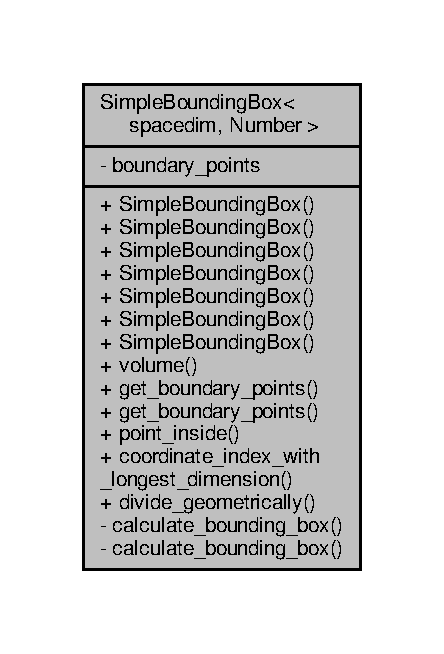
\includegraphics[width=213pt]{classSimpleBoundingBox__coll__graph}
\end{center}
\end{figure}
\subsection*{Public Member Functions}
\begin{DoxyCompactItemize}
\item 
\hyperlink{classSimpleBoundingBox_a6975b3ff39148250f0b4dfdd90194653}{Simple\+Bounding\+Box} ()
\item 
\hyperlink{classSimpleBoundingBox_a2ef944074a061d1813d46edb437706df}{Simple\+Bounding\+Box} (const Point$<$ spacedim, Number $>$ \&corner1, const Point$<$ spacedim, Number $>$ \&corner2)
\item 
\hyperlink{classSimpleBoundingBox_a75acd8fd3479b814c7e146d6948c1366}{Simple\+Bounding\+Box} (const std\+::pair$<$ Point$<$ spacedim, Number $>$, Point$<$ spacedim, Number $>$$>$ \&point\+\_\+pair)
\item 
\hyperlink{classSimpleBoundingBox_a4762c89a859a0040438b2f6b44defc79}{Simple\+Bounding\+Box} (const std\+::vector$<$ Point$<$ spacedim, Number $>$$>$ \&points)
\item 
{\footnotesize template$<$int dim$>$ }\\\hyperlink{classSimpleBoundingBox_a41f4805f49de9e15c82063927dd7ef10}{Simple\+Bounding\+Box} (const Mapping$<$ dim, spacedim $>$ \&mapping, const Do\+F\+Handler$<$ dim, spacedim $>$ \&dof\+\_\+handler)
\item 
\hyperlink{classSimpleBoundingBox_ab2568fcda9400b730d326574fa6ef58c}{Simple\+Bounding\+Box} (const std\+::vector$<$ types\+::global\+\_\+dof\+\_\+index $>$ \&dof\+\_\+indices, const std\+::vector$<$ Point$<$ spacedim, Number $>$$>$ \&all\+\_\+support\+\_\+points)
\item 
\hyperlink{classSimpleBoundingBox_adb50933d0b5a524cfa98f79fd231d557}{Simple\+Bounding\+Box} (const \hyperlink{classSimpleBoundingBox}{Simple\+Bounding\+Box}$<$ spacedim, Number $>$ \&bbox)
\item 
Number \hyperlink{classSimpleBoundingBox_a44340fd2ab10e9c05c1a88719958fee5}{volume} () const
\item 
std\+::pair$<$ Point$<$ spacedim, Number $>$, Point$<$ spacedim, Number $>$ $>$ \& \hyperlink{classSimpleBoundingBox_a1cccc2f8ebc6b5f406738f04e145b598}{get\+\_\+boundary\+\_\+points} ()
\item 
const std\+::pair$<$ Point$<$ spacedim, Number $>$, Point$<$ spacedim, Number $>$ $>$ \& \hyperlink{classSimpleBoundingBox_a7c1af5d42bfc12cd3d0c955863fe0d75}{get\+\_\+boundary\+\_\+points} () const
\item 
bool \hyperlink{classSimpleBoundingBox_af58f37fb60a09a61730797850886c39f}{point\+\_\+inside} (const Point$<$ spacedim, Number $>$ \&p) const
\item 
unsigned int \hyperlink{classSimpleBoundingBox_abc665d7750573194c9c449ef67c40113}{coordinate\+\_\+index\+\_\+with\+\_\+longest\+\_\+dimension} () const
\item 
std\+::pair$<$ \hyperlink{classSimpleBoundingBox}{Simple\+Bounding\+Box}$<$ spacedim, Number $>$, \hyperlink{classSimpleBoundingBox}{Simple\+Bounding\+Box}$<$ spacedim, Number $>$ $>$ \hyperlink{classSimpleBoundingBox_a0b8bef0a9504e22a7e2c4cc3d4ed04c4}{divide\+\_\+geometrically} () const
\end{DoxyCompactItemize}
\subsection*{Private Member Functions}
\begin{DoxyCompactItemize}
\item 
void \hyperlink{classSimpleBoundingBox_a140e9c7c01b868cfe6a5288f69522bf4}{calculate\+\_\+bounding\+\_\+box} (const std\+::vector$<$ Point$<$ spacedim, Number $>$$>$ \&points)
\item 
void \hyperlink{classSimpleBoundingBox_aafff59e6c56578638d58ca6095024bac}{calculate\+\_\+bounding\+\_\+box} (const std\+::vector$<$ types\+::global\+\_\+dof\+\_\+index $>$ \&dof\+\_\+indices, const std\+::vector$<$ Point$<$ spacedim, Number $>$$>$ \&all\+\_\+support\+\_\+points)
\end{DoxyCompactItemize}
\subsection*{Private Attributes}
\begin{DoxyCompactItemize}
\item 
std\+::pair$<$ Point$<$ spacedim, Number $>$, Point$<$ spacedim, Number $>$ $>$ \hyperlink{classSimpleBoundingBox_a066f18179d514c16ac68baa5ebd85ba5}{boundary\+\_\+points}
\end{DoxyCompactItemize}
\subsection*{Friends}
\begin{DoxyCompactItemize}
\item 
\mbox{\Hypertarget{classSimpleBoundingBox_a68f8b2f59494f354ca2bc781aa56833e}\label{classSimpleBoundingBox_a68f8b2f59494f354ca2bc781aa56833e}} 
{\footnotesize template$<$int spacedim1, typename Number1 $>$ }\\std\+::ostream \& {\bfseries operator$<$$<$} (std\+::ostream \&out, const \hyperlink{classSimpleBoundingBox}{Simple\+Bounding\+Box}$<$ spacedim1, Number1 $>$ \&bbox)
\end{DoxyCompactItemize}


\subsection{Detailed Description}
\subsubsection*{template$<$int spacedim, typename Number = double$>$\newline
class Simple\+Bounding\+Box$<$ spacedim, Number $>$}

Class implementing a simple axis-\/parallel bounding box. N.\+B. This class only has the {\ttfamily spacedim} template argument but without the {\ttfamily dim} template argument, which means an axis-\/parallel bounding box always has the same dimension as the specified space dimension. Therefore, the bounding box for a 2D surface in 3D space is still a 3D box. 

\subsection{Constructor \& Destructor Documentation}
\mbox{\Hypertarget{classSimpleBoundingBox_a6975b3ff39148250f0b4dfdd90194653}\label{classSimpleBoundingBox_a6975b3ff39148250f0b4dfdd90194653}} 
\index{Simple\+Bounding\+Box@{Simple\+Bounding\+Box}!Simple\+Bounding\+Box@{Simple\+Bounding\+Box}}
\index{Simple\+Bounding\+Box@{Simple\+Bounding\+Box}!Simple\+Bounding\+Box@{Simple\+Bounding\+Box}}
\subsubsection{\texorpdfstring{Simple\+Bounding\+Box()}{SimpleBoundingBox()}\hspace{0.1cm}{\footnotesize\ttfamily [1/7]}}
{\footnotesize\ttfamily template$<$int spacedim, typename Number $>$ \\
\hyperlink{classSimpleBoundingBox}{Simple\+Bounding\+Box}$<$ spacedim, Number $>$\+::\hyperlink{classSimpleBoundingBox}{Simple\+Bounding\+Box} (\begin{DoxyParamCaption}{ }\end{DoxyParamCaption})}

Default constructor with two boundary points being both zeros. \mbox{\Hypertarget{classSimpleBoundingBox_a2ef944074a061d1813d46edb437706df}\label{classSimpleBoundingBox_a2ef944074a061d1813d46edb437706df}} 
\index{Simple\+Bounding\+Box@{Simple\+Bounding\+Box}!Simple\+Bounding\+Box@{Simple\+Bounding\+Box}}
\index{Simple\+Bounding\+Box@{Simple\+Bounding\+Box}!Simple\+Bounding\+Box@{Simple\+Bounding\+Box}}
\subsubsection{\texorpdfstring{Simple\+Bounding\+Box()}{SimpleBoundingBox()}\hspace{0.1cm}{\footnotesize\ttfamily [2/7]}}
{\footnotesize\ttfamily template$<$int spacedim, typename Number$>$ \\
\hyperlink{classSimpleBoundingBox}{Simple\+Bounding\+Box}$<$ spacedim, Number $>$\+::\hyperlink{classSimpleBoundingBox}{Simple\+Bounding\+Box} (\begin{DoxyParamCaption}\item[{const Point$<$ spacedim, Number $>$ \&}]{corner1,  }\item[{const Point$<$ spacedim, Number $>$ \&}]{corner2 }\end{DoxyParamCaption})}

Constructor from two corner points. \mbox{\Hypertarget{classSimpleBoundingBox_a75acd8fd3479b814c7e146d6948c1366}\label{classSimpleBoundingBox_a75acd8fd3479b814c7e146d6948c1366}} 
\index{Simple\+Bounding\+Box@{Simple\+Bounding\+Box}!Simple\+Bounding\+Box@{Simple\+Bounding\+Box}}
\index{Simple\+Bounding\+Box@{Simple\+Bounding\+Box}!Simple\+Bounding\+Box@{Simple\+Bounding\+Box}}
\subsubsection{\texorpdfstring{Simple\+Bounding\+Box()}{SimpleBoundingBox()}\hspace{0.1cm}{\footnotesize\ttfamily [3/7]}}
{\footnotesize\ttfamily template$<$int spacedim, typename Number$>$ \\
\hyperlink{classSimpleBoundingBox}{Simple\+Bounding\+Box}$<$ spacedim, Number $>$\+::\hyperlink{classSimpleBoundingBox}{Simple\+Bounding\+Box} (\begin{DoxyParamCaption}\item[{const std\+::pair$<$ Point$<$ spacedim, Number $>$, Point$<$ spacedim, Number $>$$>$ \&}]{point\+\_\+pair }\end{DoxyParamCaption})}

Constructor from a pair of corner points. 
\begin{DoxyParams}{Parameters}
{\em point\+\_\+pair} & \\
\hline
\end{DoxyParams}
\mbox{\Hypertarget{classSimpleBoundingBox_a4762c89a859a0040438b2f6b44defc79}\label{classSimpleBoundingBox_a4762c89a859a0040438b2f6b44defc79}} 
\index{Simple\+Bounding\+Box@{Simple\+Bounding\+Box}!Simple\+Bounding\+Box@{Simple\+Bounding\+Box}}
\index{Simple\+Bounding\+Box@{Simple\+Bounding\+Box}!Simple\+Bounding\+Box@{Simple\+Bounding\+Box}}
\subsubsection{\texorpdfstring{Simple\+Bounding\+Box()}{SimpleBoundingBox()}\hspace{0.1cm}{\footnotesize\ttfamily [4/7]}}
{\footnotesize\ttfamily template$<$int spacedim, typename Number$>$ \\
\hyperlink{classSimpleBoundingBox}{Simple\+Bounding\+Box}$<$ spacedim, Number $>$\+::\hyperlink{classSimpleBoundingBox}{Simple\+Bounding\+Box} (\begin{DoxyParamCaption}\item[{const std\+::vector$<$ Point$<$ spacedim, Number $>$$>$ \&}]{points }\end{DoxyParamCaption})}

Constructor from a vector of points. \mbox{\Hypertarget{classSimpleBoundingBox_a41f4805f49de9e15c82063927dd7ef10}\label{classSimpleBoundingBox_a41f4805f49de9e15c82063927dd7ef10}} 
\index{Simple\+Bounding\+Box@{Simple\+Bounding\+Box}!Simple\+Bounding\+Box@{Simple\+Bounding\+Box}}
\index{Simple\+Bounding\+Box@{Simple\+Bounding\+Box}!Simple\+Bounding\+Box@{Simple\+Bounding\+Box}}
\subsubsection{\texorpdfstring{Simple\+Bounding\+Box()}{SimpleBoundingBox()}\hspace{0.1cm}{\footnotesize\ttfamily [5/7]}}
{\footnotesize\ttfamily template$<$int spacedim, typename Number $>$ \\
template$<$int dim$>$ \\
\hyperlink{classSimpleBoundingBox}{Simple\+Bounding\+Box}$<$ spacedim, Number $>$\+::\hyperlink{classSimpleBoundingBox}{Simple\+Bounding\+Box} (\begin{DoxyParamCaption}\item[{const Mapping$<$ dim, spacedim $>$ \&}]{mapping,  }\item[{const Do\+F\+Handler$<$ dim, spacedim $>$ \&}]{dof\+\_\+handler }\end{DoxyParamCaption})}

Constructor from a {\ttfamily Mapping} and a {\ttfamily Do\+F\+Handler}. N.\+B. This is a template constructor with the argument dim as manifold dimension. The resulted bounding box contains the support points associated with all Do\+Fs within the Do\+F\+Handler. \mbox{\Hypertarget{classSimpleBoundingBox_ab2568fcda9400b730d326574fa6ef58c}\label{classSimpleBoundingBox_ab2568fcda9400b730d326574fa6ef58c}} 
\index{Simple\+Bounding\+Box@{Simple\+Bounding\+Box}!Simple\+Bounding\+Box@{Simple\+Bounding\+Box}}
\index{Simple\+Bounding\+Box@{Simple\+Bounding\+Box}!Simple\+Bounding\+Box@{Simple\+Bounding\+Box}}
\subsubsection{\texorpdfstring{Simple\+Bounding\+Box()}{SimpleBoundingBox()}\hspace{0.1cm}{\footnotesize\ttfamily [6/7]}}
{\footnotesize\ttfamily template$<$int spacedim, typename Number$>$ \\
\hyperlink{classSimpleBoundingBox}{Simple\+Bounding\+Box}$<$ spacedim, Number $>$\+::\hyperlink{classSimpleBoundingBox}{Simple\+Bounding\+Box} (\begin{DoxyParamCaption}\item[{const std\+::vector$<$ types\+::global\+\_\+dof\+\_\+index $>$ \&}]{dof\+\_\+indices,  }\item[{const std\+::vector$<$ Point$<$ spacedim, Number $>$$>$ \&}]{all\+\_\+support\+\_\+points }\end{DoxyParamCaption})}

Constructor from a specified DoF index set. The support point coordinates for all Do\+Fs have been placed into {\ttfamily all\+\_\+support\+\_\+points}. 
\begin{DoxyParams}{Parameters}
{\em dof\+\_\+indices} & The DoF index set, for which the bounding box is to be generated. \\
\hline
{\em all\+\_\+support\+\_\+points} & The const reference to the list of all support points associated with a Do\+F\+Handler. \\
\hline
\end{DoxyParams}
\mbox{\Hypertarget{classSimpleBoundingBox_adb50933d0b5a524cfa98f79fd231d557}\label{classSimpleBoundingBox_adb50933d0b5a524cfa98f79fd231d557}} 
\index{Simple\+Bounding\+Box@{Simple\+Bounding\+Box}!Simple\+Bounding\+Box@{Simple\+Bounding\+Box}}
\index{Simple\+Bounding\+Box@{Simple\+Bounding\+Box}!Simple\+Bounding\+Box@{Simple\+Bounding\+Box}}
\subsubsection{\texorpdfstring{Simple\+Bounding\+Box()}{SimpleBoundingBox()}\hspace{0.1cm}{\footnotesize\ttfamily [7/7]}}
{\footnotesize\ttfamily template$<$int spacedim, typename Number$>$ \\
\hyperlink{classSimpleBoundingBox}{Simple\+Bounding\+Box}$<$ spacedim, Number $>$\+::\hyperlink{classSimpleBoundingBox}{Simple\+Bounding\+Box} (\begin{DoxyParamCaption}\item[{const \hyperlink{classSimpleBoundingBox}{Simple\+Bounding\+Box}$<$ spacedim, Number $>$ \&}]{bbox }\end{DoxyParamCaption})}

Copy constructor 

\subsection{Member Function Documentation}
\mbox{\Hypertarget{classSimpleBoundingBox_a140e9c7c01b868cfe6a5288f69522bf4}\label{classSimpleBoundingBox_a140e9c7c01b868cfe6a5288f69522bf4}} 
\index{Simple\+Bounding\+Box@{Simple\+Bounding\+Box}!calculate\+\_\+bounding\+\_\+box@{calculate\+\_\+bounding\+\_\+box}}
\index{calculate\+\_\+bounding\+\_\+box@{calculate\+\_\+bounding\+\_\+box}!Simple\+Bounding\+Box@{Simple\+Bounding\+Box}}
\subsubsection{\texorpdfstring{calculate\+\_\+bounding\+\_\+box()}{calculate\_bounding\_box()}\hspace{0.1cm}{\footnotesize\ttfamily [1/2]}}
{\footnotesize\ttfamily template$<$int spacedim, typename Number$>$ \\
void \hyperlink{classSimpleBoundingBox}{Simple\+Bounding\+Box}$<$ spacedim, Number $>$\+::calculate\+\_\+bounding\+\_\+box (\begin{DoxyParamCaption}\item[{const std\+::vector$<$ Point$<$ spacedim, Number $>$$>$ \&}]{points }\end{DoxyParamCaption})\hspace{0.3cm}{\ttfamily [private]}}

Calculate the bounding box from a list of points. Initialize the two boundary points to be the first point in the list.

Calculate the minimum and the maximum coordinate for each dimension.

Referenced by Simple\+Bounding\+Box$<$ spacedim, double $>$\+::\+Simple\+Bounding\+Box().

\mbox{\Hypertarget{classSimpleBoundingBox_aafff59e6c56578638d58ca6095024bac}\label{classSimpleBoundingBox_aafff59e6c56578638d58ca6095024bac}} 
\index{Simple\+Bounding\+Box@{Simple\+Bounding\+Box}!calculate\+\_\+bounding\+\_\+box@{calculate\+\_\+bounding\+\_\+box}}
\index{calculate\+\_\+bounding\+\_\+box@{calculate\+\_\+bounding\+\_\+box}!Simple\+Bounding\+Box@{Simple\+Bounding\+Box}}
\subsubsection{\texorpdfstring{calculate\+\_\+bounding\+\_\+box()}{calculate\_bounding\_box()}\hspace{0.1cm}{\footnotesize\ttfamily [2/2]}}
{\footnotesize\ttfamily template$<$int spacedim, typename Number$>$ \\
void \hyperlink{classSimpleBoundingBox}{Simple\+Bounding\+Box}$<$ spacedim, Number $>$\+::calculate\+\_\+bounding\+\_\+box (\begin{DoxyParamCaption}\item[{const std\+::vector$<$ types\+::global\+\_\+dof\+\_\+index $>$ \&}]{dof\+\_\+indices,  }\item[{const std\+::vector$<$ Point$<$ spacedim, Number $>$$>$ \&}]{all\+\_\+support\+\_\+points }\end{DoxyParamCaption})\hspace{0.3cm}{\ttfamily [private]}}

Calculate the bounding box from a list of DoF indices. 
\begin{DoxyParams}{Parameters}
{\em dof\+\_\+indices} & The DoF index set. \\
\hline
{\em all\+\_\+support\+\_\+points} & The const reference to the list of all support points associated with a Do\+F\+Handler. \\
\hline
\end{DoxyParams}
Initialize the two boundary points to be the point associated with the first DoF index.

Calculate the minimum and the maximum coordinate for each dimension.\mbox{\Hypertarget{classSimpleBoundingBox_abc665d7750573194c9c449ef67c40113}\label{classSimpleBoundingBox_abc665d7750573194c9c449ef67c40113}} 
\index{Simple\+Bounding\+Box@{Simple\+Bounding\+Box}!coordinate\+\_\+index\+\_\+with\+\_\+longest\+\_\+dimension@{coordinate\+\_\+index\+\_\+with\+\_\+longest\+\_\+dimension}}
\index{coordinate\+\_\+index\+\_\+with\+\_\+longest\+\_\+dimension@{coordinate\+\_\+index\+\_\+with\+\_\+longest\+\_\+dimension}!Simple\+Bounding\+Box@{Simple\+Bounding\+Box}}
\subsubsection{\texorpdfstring{coordinate\+\_\+index\+\_\+with\+\_\+longest\+\_\+dimension()}{coordinate\_index\_with\_longest\_dimension()}}
{\footnotesize\ttfamily template$<$int spacedim, typename Number $>$ \\
unsigned int \hyperlink{classSimpleBoundingBox}{Simple\+Bounding\+Box}$<$ spacedim, Number $>$\+::coordinate\+\_\+index\+\_\+with\+\_\+longest\+\_\+dimension (\begin{DoxyParamCaption}{ }\end{DoxyParamCaption}) const}

Get the index to the coordinate component, which has the longest dimension. \begin{DoxyReturn}{Returns}
Index to the coordinate component, which should be in the range $[0, {\rm spacedim})$. 
\end{DoxyReturn}


Referenced by Simple\+Bounding\+Box$<$ spacedim, double $>$\+::divide\+\_\+geometrically().

\mbox{\Hypertarget{classSimpleBoundingBox_a0b8bef0a9504e22a7e2c4cc3d4ed04c4}\label{classSimpleBoundingBox_a0b8bef0a9504e22a7e2c4cc3d4ed04c4}} 
\index{Simple\+Bounding\+Box@{Simple\+Bounding\+Box}!divide\+\_\+geometrically@{divide\+\_\+geometrically}}
\index{divide\+\_\+geometrically@{divide\+\_\+geometrically}!Simple\+Bounding\+Box@{Simple\+Bounding\+Box}}
\subsubsection{\texorpdfstring{divide\+\_\+geometrically()}{divide\_geometrically()}}
{\footnotesize\ttfamily template$<$int spacedim, typename Number $>$ \\
std\+::pair$<$ \hyperlink{classSimpleBoundingBox}{Simple\+Bounding\+Box}$<$ spacedim, Number $>$, \hyperlink{classSimpleBoundingBox}{Simple\+Bounding\+Box}$<$ spacedim, Number $>$ $>$ \hyperlink{classSimpleBoundingBox}{Simple\+Bounding\+Box}$<$ spacedim, Number $>$\+::divide\+\_\+geometrically (\begin{DoxyParamCaption}{ }\end{DoxyParamCaption}) const}

Bisect the bounding box along the longest coordinate direction. \begin{DoxyReturn}{Returns}

\end{DoxyReturn}
Calculate the coordinate index which has the longest dimension.

Modify the {\ttfamily coordinate\+\_\+index} \textquotesingle{}th coordinate of the top corner point in the first box.

Modify the {\ttfamily coordinate\+\_\+index} \textquotesingle{}th coordinate of the bottom corner point in the second box.

Referenced by Cluster\+Tree$<$ spacedim, double $>$\+::partition\+\_\+from\+\_\+cluster\+\_\+node().

\mbox{\Hypertarget{classSimpleBoundingBox_a1cccc2f8ebc6b5f406738f04e145b598}\label{classSimpleBoundingBox_a1cccc2f8ebc6b5f406738f04e145b598}} 
\index{Simple\+Bounding\+Box@{Simple\+Bounding\+Box}!get\+\_\+boundary\+\_\+points@{get\+\_\+boundary\+\_\+points}}
\index{get\+\_\+boundary\+\_\+points@{get\+\_\+boundary\+\_\+points}!Simple\+Bounding\+Box@{Simple\+Bounding\+Box}}
\subsubsection{\texorpdfstring{get\+\_\+boundary\+\_\+points()}{get\_boundary\_points()}\hspace{0.1cm}{\footnotesize\ttfamily [1/2]}}
{\footnotesize\ttfamily template$<$int spacedim, typename Number $>$ \\
std\+::pair$<$ Point$<$ spacedim, Number $>$, Point$<$ spacedim, Number $>$ $>$ \& \hyperlink{classSimpleBoundingBox}{Simple\+Bounding\+Box}$<$ spacedim, Number $>$\+::get\+\_\+boundary\+\_\+points (\begin{DoxyParamCaption}{ }\end{DoxyParamCaption})}

Get the two corner points of the bounding box (mutable version). \begin{DoxyReturn}{Returns}
The reference to the pair of corner points. The point with a smaller coordinate in each dimension is the first. 
\end{DoxyReturn}


Referenced by Simple\+Bounding\+Box$<$ spacedim, double $>$\+::divide\+\_\+geometrically().

\mbox{\Hypertarget{classSimpleBoundingBox_a7c1af5d42bfc12cd3d0c955863fe0d75}\label{classSimpleBoundingBox_a7c1af5d42bfc12cd3d0c955863fe0d75}} 
\index{Simple\+Bounding\+Box@{Simple\+Bounding\+Box}!get\+\_\+boundary\+\_\+points@{get\+\_\+boundary\+\_\+points}}
\index{get\+\_\+boundary\+\_\+points@{get\+\_\+boundary\+\_\+points}!Simple\+Bounding\+Box@{Simple\+Bounding\+Box}}
\subsubsection{\texorpdfstring{get\+\_\+boundary\+\_\+points()}{get\_boundary\_points()}\hspace{0.1cm}{\footnotesize\ttfamily [2/2]}}
{\footnotesize\ttfamily template$<$int spacedim, typename Number $>$ \\
const std\+::pair$<$ Point$<$ spacedim, Number $>$, Point$<$ spacedim, Number $>$ $>$ \& \hyperlink{classSimpleBoundingBox}{Simple\+Bounding\+Box}$<$ spacedim, Number $>$\+::get\+\_\+boundary\+\_\+points (\begin{DoxyParamCaption}{ }\end{DoxyParamCaption}) const}

Get the two corner points of the bounding box (const version). \begin{DoxyReturn}{Returns}
The const reference to the pair of corner points. The point with a smaller coordinate in each dimension is the first. 
\end{DoxyReturn}
\mbox{\Hypertarget{classSimpleBoundingBox_af58f37fb60a09a61730797850886c39f}\label{classSimpleBoundingBox_af58f37fb60a09a61730797850886c39f}} 
\index{Simple\+Bounding\+Box@{Simple\+Bounding\+Box}!point\+\_\+inside@{point\+\_\+inside}}
\index{point\+\_\+inside@{point\+\_\+inside}!Simple\+Bounding\+Box@{Simple\+Bounding\+Box}}
\subsubsection{\texorpdfstring{point\+\_\+inside()}{point\_inside()}}
{\footnotesize\ttfamily template$<$int spacedim, typename Number$>$ \\
bool \hyperlink{classSimpleBoundingBox}{Simple\+Bounding\+Box}$<$ spacedim, Number $>$\+::point\+\_\+inside (\begin{DoxyParamCaption}\item[{const Point$<$ spacedim, Number $>$ \&}]{p }\end{DoxyParamCaption}) const}

Determine if a given point lies within the bounding box. Make a predicate on if the point lies outside the bounding box.\mbox{\Hypertarget{classSimpleBoundingBox_a44340fd2ab10e9c05c1a88719958fee5}\label{classSimpleBoundingBox_a44340fd2ab10e9c05c1a88719958fee5}} 
\index{Simple\+Bounding\+Box@{Simple\+Bounding\+Box}!volume@{volume}}
\index{volume@{volume}!Simple\+Bounding\+Box@{Simple\+Bounding\+Box}}
\subsubsection{\texorpdfstring{volume()}{volume()}}
{\footnotesize\ttfamily template$<$int spacedim, typename Number $>$ \\
Number \hyperlink{classSimpleBoundingBox}{Simple\+Bounding\+Box}$<$ spacedim, Number $>$\+::volume (\begin{DoxyParamCaption}{ }\end{DoxyParamCaption}) const}

Calculate the volume of the bounding box. \begin{DoxyReturn}{Returns}
Volume of the bounding box. 
\end{DoxyReturn}


\subsection{Member Data Documentation}
\mbox{\Hypertarget{classSimpleBoundingBox_a066f18179d514c16ac68baa5ebd85ba5}\label{classSimpleBoundingBox_a066f18179d514c16ac68baa5ebd85ba5}} 
\index{Simple\+Bounding\+Box@{Simple\+Bounding\+Box}!boundary\+\_\+points@{boundary\+\_\+points}}
\index{boundary\+\_\+points@{boundary\+\_\+points}!Simple\+Bounding\+Box@{Simple\+Bounding\+Box}}
\subsubsection{\texorpdfstring{boundary\+\_\+points}{boundary\_points}}
{\footnotesize\ttfamily template$<$int spacedim, typename Number = double$>$ \\
std\+::pair$<$Point$<$spacedim, Number$>$, Point$<$spacedim, Number$>$ $>$ \hyperlink{classSimpleBoundingBox}{Simple\+Bounding\+Box}$<$ spacedim, Number $>$\+::boundary\+\_\+points\hspace{0.3cm}{\ttfamily [private]}}

Two corner points of the bounding box. The point in the pair is the bottom corner, i.\+e. it has a smaller component coordinate in each dimension; while the second point is the top corner. 

Referenced by Simple\+Bounding\+Box$<$ spacedim, double $>$\+::calculate\+\_\+bounding\+\_\+box(), Simple\+Bounding\+Box$<$ spacedim, double $>$\+::coordinate\+\_\+index\+\_\+with\+\_\+longest\+\_\+dimension(), Simple\+Bounding\+Box$<$ spacedim, double $>$\+::get\+\_\+boundary\+\_\+points(), Simple\+Bounding\+Box$<$ spacedim, double $>$\+::point\+\_\+inside(), and Simple\+Bounding\+Box$<$ spacedim, double $>$\+::volume().



The documentation for this class was generated from the following file\+:\begin{DoxyCompactItemize}
\item 
/home/jihuan/\+Projects/deal.\+ii/program/dealii-\/9.\+1.\+1/examples/laplace-\/bem/include/simple\+\_\+bounding\+\_\+box.\+h\end{DoxyCompactItemize}

\hypertarget{classLaplaceBEM_1_1LaplaceKernel_1_1SingleLayerKernel}{}\section{Laplace\+B\+EM\+:\+:Laplace\+Kernel\+:\+:Single\+Layer\+Kernel$<$ dim, Range\+Number\+Type $>$ Class Template Reference}
\label{classLaplaceBEM_1_1LaplaceKernel_1_1SingleLayerKernel}\index{Laplace\+B\+E\+M\+::\+Laplace\+Kernel\+::\+Single\+Layer\+Kernel$<$ dim, Range\+Number\+Type $>$@{Laplace\+B\+E\+M\+::\+Laplace\+Kernel\+::\+Single\+Layer\+Kernel$<$ dim, Range\+Number\+Type $>$}}


{\ttfamily \#include $<$laplace\+\_\+bem.\+h$>$}



Inheritance diagram for Laplace\+B\+EM\+:\+:Laplace\+Kernel\+:\+:Single\+Layer\+Kernel$<$ dim, Range\+Number\+Type $>$\+:\nopagebreak
\begin{figure}[H]
\begin{center}
\leavevmode
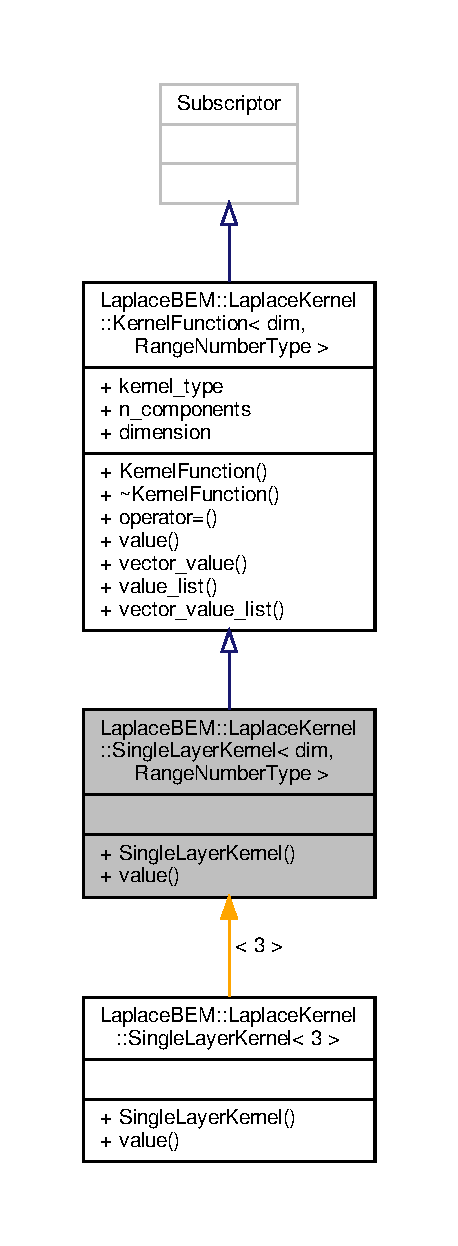
\includegraphics[height=550pt]{classLaplaceBEM_1_1LaplaceKernel_1_1SingleLayerKernel__inherit__graph}
\end{center}
\end{figure}


Collaboration diagram for Laplace\+B\+EM\+:\+:Laplace\+Kernel\+:\+:Single\+Layer\+Kernel$<$ dim, Range\+Number\+Type $>$\+:\nopagebreak
\begin{figure}[H]
\begin{center}
\leavevmode
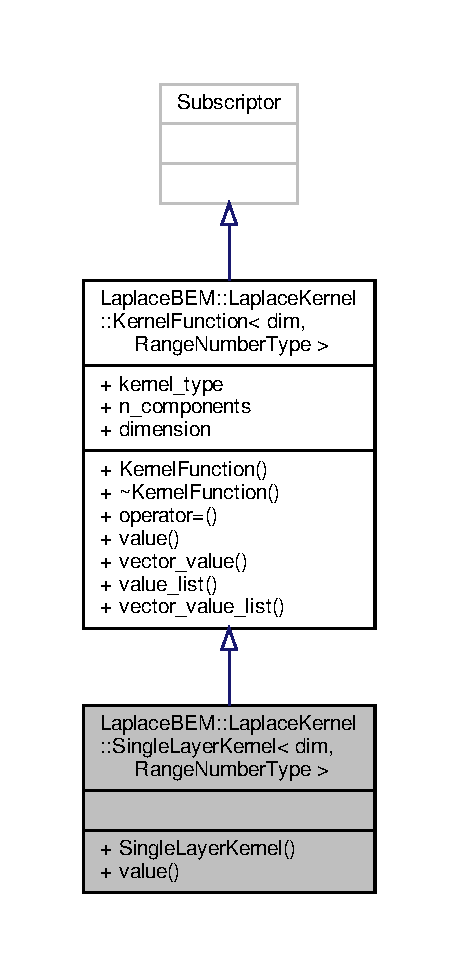
\includegraphics[width=220pt]{classLaplaceBEM_1_1LaplaceKernel_1_1SingleLayerKernel__coll__graph}
\end{center}
\end{figure}
\subsection*{Public Member Functions}
\begin{DoxyCompactItemize}
\item 
\mbox{\Hypertarget{classLaplaceBEM_1_1LaplaceKernel_1_1SingleLayerKernel_a657e04bd67d8c33adeea1b9d282d6136}\label{classLaplaceBEM_1_1LaplaceKernel_1_1SingleLayerKernel_a657e04bd67d8c33adeea1b9d282d6136}} 
virtual Range\+Number\+Type {\bfseries value} (const Point$<$ dim $>$ \&x, const Point$<$ dim $>$ \&y, const Tensor$<$ 1, dim $>$ \&nx, const Tensor$<$ 1, dim $>$ \&ny, const unsigned int component=0) const override
\end{DoxyCompactItemize}
\subsection*{Additional Inherited Members}


\subsection{Detailed Description}
\subsubsection*{template$<$int dim, typename Range\+Number\+Type = double$>$\newline
class Laplace\+B\+E\+M\+::\+Laplace\+Kernel\+::\+Single\+Layer\+Kernel$<$ dim, Range\+Number\+Type $>$}

Single layer kernel. 

The documentation for this class was generated from the following file\+:\begin{DoxyCompactItemize}
\item 
/home/jihuan/\+Projects/deal.\+ii/program/dealii-\/9.\+1.\+1/examples/laplace-\/bem/include/\hyperlink{laplace__bem_8h}{laplace\+\_\+bem.\+h}\end{DoxyCompactItemize}

\hypertarget{classTreeNode}{}\section{Tree\+Node$<$ T, N $>$ Class Template Reference}
\label{classTreeNode}\index{Tree\+Node$<$ T, N $>$@{Tree\+Node$<$ T, N $>$}}


Class for general tree node.  




{\ttfamily \#include $<$tree.\+h$>$}



Inheritance diagram for Tree\+Node$<$ T, N $>$\+:\nopagebreak
\begin{figure}[H]
\begin{center}
\leavevmode
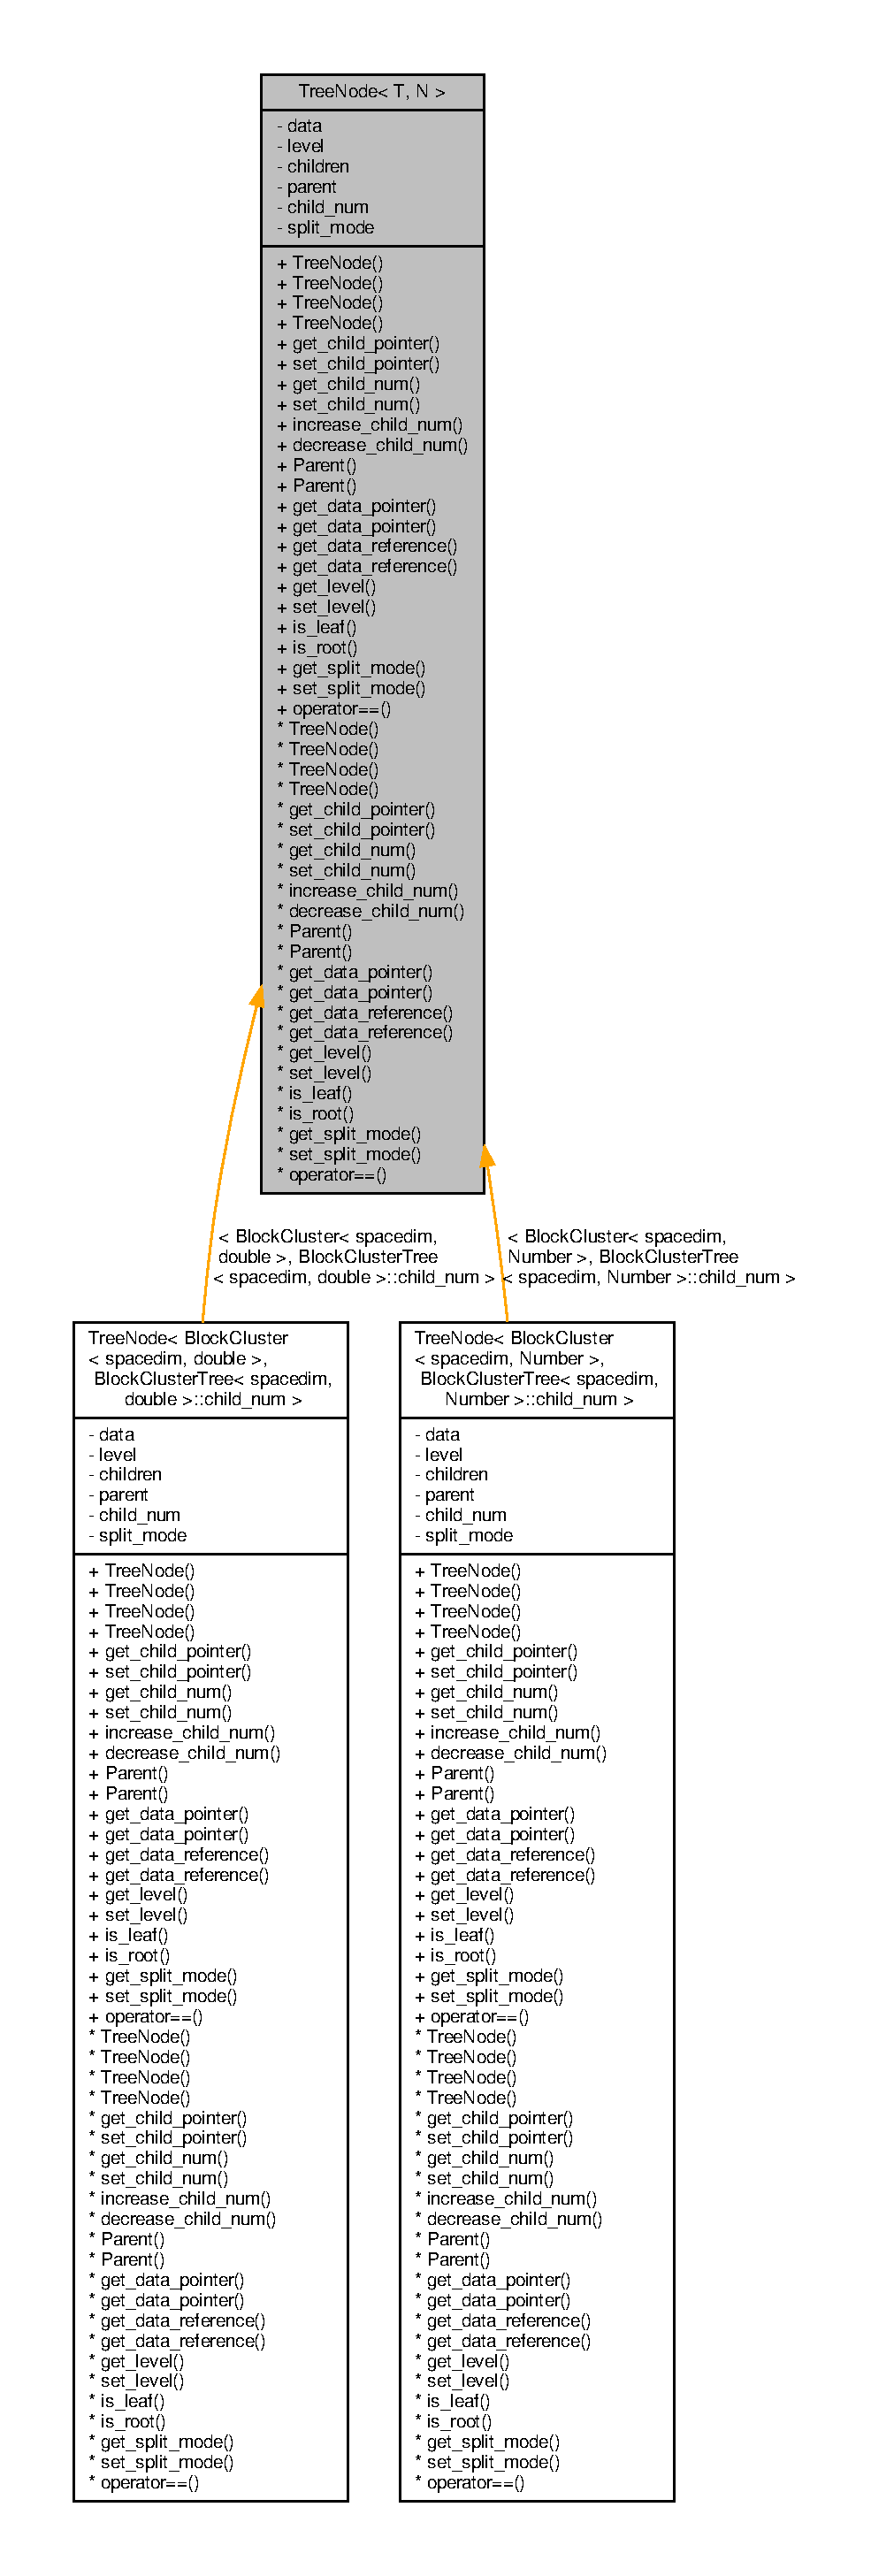
\includegraphics[height=550pt]{classTreeNode__inherit__graph}
\end{center}
\end{figure}


Collaboration diagram for Tree\+Node$<$ T, N $>$\+:\nopagebreak
\begin{figure}[H]
\begin{center}
\leavevmode
\includegraphics[height=550pt]{classTreeNode__coll__graph}
\end{center}
\end{figure}
\subsection*{Public Member Functions}
\textbf{ }\par
\begin{DoxyCompactItemize}
\item 
\hyperlink{classTreeNode_a0cd82abd44bd197539bbd045aeef30d1}{Tree\+Node} ()
\item 
\hyperlink{classTreeNode_a6549fc1c54bafa84fb41c850f1d4586e}{Tree\+Node} (const T \&data)
\item 
\hyperlink{classTreeNode_ad5a724100f06f73f002007a2e433932c}{Tree\+Node} (const T \&data, unsigned int level, const std\+::array$<$ \hyperlink{classTreeNode}{Tree\+Node} $\ast$, N $>$ \&children, \hyperlink{classTreeNode}{Tree\+Node} $\ast$parent=nullptr, \hyperlink{tree_8h_a922ca07db9633957939f697a65aff11d}{Tree\+Node\+Split\+Mode} split\+\_\+mode=Unsplit\+Mode)
\item 
\hyperlink{classTreeNode_af05018d87f64710f41df36bfedd562f3}{Tree\+Node} (const \hyperlink{classTreeNode}{Tree\+Node} \&node)
\item 
\hyperlink{classTreeNode}{Tree\+Node} $\ast$ \hyperlink{classTreeNode_ad3b1833452c787d2146a4beb3587c531}{get\+\_\+child\+\_\+pointer} (std\+::size\+\_\+t index) const
\item 
void \hyperlink{classTreeNode_a3d2f374424a723cb72409857ee5237bc}{set\+\_\+child\+\_\+pointer} (std\+::size\+\_\+t index, const \hyperlink{classTreeNode}{Tree\+Node} $\ast$pointer)
\item 
unsigned int \hyperlink{classTreeNode_a077cb5cc974f94ff431c69cc2ca5957f}{get\+\_\+child\+\_\+num} () const
\item 
void \hyperlink{classTreeNode_a68c80783a2900d01a37fc33f14951e66}{set\+\_\+child\+\_\+num} (const unsigned int \hyperlink{classTreeNode_a9fc9333a3e4e05ae878a844370c17888}{child\+\_\+num})
\item 
void \hyperlink{classTreeNode_a1d471684d9c06b5721217fb55182bdeb}{increase\+\_\+child\+\_\+num} (const unsigned int incr\+\_\+num=1)
\item 
void \hyperlink{classTreeNode_a25426ded0c574843912b36216b30dc5e}{decrease\+\_\+child\+\_\+num} (const unsigned int decr\+\_\+num=1)
\item 
\hyperlink{classTreeNode}{Tree\+Node} $\ast$ \hyperlink{classTreeNode_a66c83bfefdb235d5cb4a299eb5044465}{Parent} (void) const
\item 
void \hyperlink{classTreeNode_a412b1980ecabb954901391b73332e657}{Parent} (const \hyperlink{classTreeNode}{Tree\+Node} $\ast$node\+\_\+pointer)
\item 
T $\ast$ \hyperlink{classTreeNode_aaa2ba047902c4e2fccffe3424a0c665b}{get\+\_\+data\+\_\+pointer} ()
\item 
const T $\ast$ \hyperlink{classTreeNode_ac6894ba6488ee38978ef2476366f6318}{get\+\_\+data\+\_\+pointer} () const
\item 
T \& \hyperlink{classTreeNode_a7bf414928c965e707e0246f7a90a747d}{get\+\_\+data\+\_\+reference} ()
\item 
const T \& \hyperlink{classTreeNode_ab051909179e64f75d4588b4618049193}{get\+\_\+data\+\_\+reference} () const
\item 
unsigned int \hyperlink{classTreeNode_acdf29b3bf8f5f9c5e04baaa9fd71fb4c}{get\+\_\+level} () const
\item 
void \hyperlink{classTreeNode_a67e5762f796247c38f4a2560c1250b11}{set\+\_\+level} (const unsigned int level)
\item 
bool \hyperlink{classTreeNode_a64bf0bc987b1abe5ba10cdf32f093b58}{is\+\_\+leaf} () const
\item 
bool \hyperlink{classTreeNode_ad2eb3a4d2a8d9dad252ee721bab24655}{is\+\_\+root} () const
\item 
\hyperlink{tree_8h_a922ca07db9633957939f697a65aff11d}{Tree\+Node\+Split\+Mode} \hyperlink{classTreeNode_a219944254f78755b181cad0ee621835f}{get\+\_\+split\+\_\+mode} () const
\item 
void \hyperlink{classTreeNode_a0aec2b9142e931aaaa15d1c451ed9b46}{set\+\_\+split\+\_\+mode} (\hyperlink{tree_8h_a922ca07db9633957939f697a65aff11d}{Tree\+Node\+Split\+Mode} split\+\_\+mode)
\item 
bool \hyperlink{classTreeNode_a9446085d81c4266ca30a384001f55b12}{operator==} (const \hyperlink{classTreeNode}{Tree\+Node}$<$ T, N $>$ \&node) const
\end{DoxyCompactItemize}

\subsection*{Private Attributes}
\begin{DoxyCompactItemize}
\item 
\mbox{\Hypertarget{classTreeNode_af44009d5463e65cc0e2d33223b849372}\label{classTreeNode_af44009d5463e65cc0e2d33223b849372}} 
T {\bfseries data}
\item 
\mbox{\Hypertarget{classTreeNode_a14271b0c2f081e59bb268a9989b3b1af}\label{classTreeNode_a14271b0c2f081e59bb268a9989b3b1af}} 
unsigned int {\bfseries level}
\item 
\mbox{\Hypertarget{classTreeNode_a27778d09f91e69ac9847d7910b1c2da7}\label{classTreeNode_a27778d09f91e69ac9847d7910b1c2da7}} 
std\+::array$<$ \hyperlink{classTreeNode}{Tree\+Node} $\ast$, N $>$ {\bfseries children}
\item 
\mbox{\Hypertarget{classTreeNode_aa3771a67ab22185807e8d7a1643ac1c4}\label{classTreeNode_aa3771a67ab22185807e8d7a1643ac1c4}} 
\hyperlink{classTreeNode}{Tree\+Node} $\ast$ {\bfseries parent}
\item 
unsigned int \hyperlink{classTreeNode_a9fc9333a3e4e05ae878a844370c17888}{child\+\_\+num}
\item 
\mbox{\Hypertarget{classTreeNode_ad4c2701845efda6aedd8433cfc0ce363}\label{classTreeNode_ad4c2701845efda6aedd8433cfc0ce363}} 
\hyperlink{tree_8h_a922ca07db9633957939f697a65aff11d}{Tree\+Node\+Split\+Mode} {\bfseries split\+\_\+mode}
\end{DoxyCompactItemize}


\subsection{Detailed Description}
\subsubsection*{template$<$typename T, std\+::size\+\_\+t N$>$\newline
class Tree\+Node$<$ T, N $>$}

Class for general tree node. 

This general tree node can contains any but {\itshape fixed} number of children. {\ttfamily T} is the type of the data held by the node. {\ttfamily N} is the number of children belong to the node. 

\subsection{Constructor \& Destructor Documentation}
\mbox{\Hypertarget{classTreeNode_a0cd82abd44bd197539bbd045aeef30d1}\label{classTreeNode_a0cd82abd44bd197539bbd045aeef30d1}} 
\index{Tree\+Node@{Tree\+Node}!Tree\+Node@{Tree\+Node}}
\index{Tree\+Node@{Tree\+Node}!Tree\+Node@{Tree\+Node}}
\subsubsection{\texorpdfstring{Tree\+Node()}{TreeNode()}\hspace{0.1cm}{\footnotesize\ttfamily [1/4]}}
{\footnotesize\ttfamily template$<$typename T , std\+::size\+\_\+t N$>$ \\
\hyperlink{classTreeNode}{Tree\+Node}$<$ T, N $>$\+::\hyperlink{classTreeNode}{Tree\+Node} (\begin{DoxyParamCaption}{ }\end{DoxyParamCaption})}

Default constructor \mbox{\Hypertarget{classTreeNode_a6549fc1c54bafa84fb41c850f1d4586e}\label{classTreeNode_a6549fc1c54bafa84fb41c850f1d4586e}} 
\index{Tree\+Node@{Tree\+Node}!Tree\+Node@{Tree\+Node}}
\index{Tree\+Node@{Tree\+Node}!Tree\+Node@{Tree\+Node}}
\subsubsection{\texorpdfstring{Tree\+Node()}{TreeNode()}\hspace{0.1cm}{\footnotesize\ttfamily [2/4]}}
{\footnotesize\ttfamily template$<$typename T, std\+::size\+\_\+t N$>$ \\
\hyperlink{classTreeNode}{Tree\+Node}$<$ T, N $>$\+::\hyperlink{classTreeNode}{Tree\+Node} (\begin{DoxyParamCaption}\item[{const T \&}]{data }\end{DoxyParamCaption})}

Constructor from the given data without children. \mbox{\Hypertarget{classTreeNode_ad5a724100f06f73f002007a2e433932c}\label{classTreeNode_ad5a724100f06f73f002007a2e433932c}} 
\index{Tree\+Node@{Tree\+Node}!Tree\+Node@{Tree\+Node}}
\index{Tree\+Node@{Tree\+Node}!Tree\+Node@{Tree\+Node}}
\subsubsection{\texorpdfstring{Tree\+Node()}{TreeNode()}\hspace{0.1cm}{\footnotesize\ttfamily [3/4]}}
{\footnotesize\ttfamily template$<$typename T, std\+::size\+\_\+t N$>$ \\
\hyperlink{classTreeNode}{Tree\+Node}$<$ T, N $>$\+::\hyperlink{classTreeNode}{Tree\+Node} (\begin{DoxyParamCaption}\item[{const T \&}]{data,  }\item[{unsigned int}]{level,  }\item[{const std\+::array$<$ \hyperlink{classTreeNode}{Tree\+Node}$<$ T, N $>$ $\ast$, N $>$ \&}]{children,  }\item[{\hyperlink{classTreeNode}{Tree\+Node}$<$ T, N $>$ $\ast$}]{parent = {\ttfamily nullptr},  }\item[{\hyperlink{tree_8h_a922ca07db9633957939f697a65aff11d}{Tree\+Node\+Split\+Mode}}]{split\+\_\+mode = {\ttfamily UnsplitMode} }\end{DoxyParamCaption})}

Constructor from the given data.

N.\+B. The number of children of the parent node will automatically be incremented, because the current node is associated with this parent. Count the total number of nonempty children.

When the tree node is split into four children, this is a cross splitting mode. Otherwise, {\ttfamily split\+\_\+mode} is temporarily kept at {\ttfamily Unsplit\+Mode}, which will further be set from outside.

Increment the {\ttfamily child\+\_\+num} of the parent node.\mbox{\Hypertarget{classTreeNode_af05018d87f64710f41df36bfedd562f3}\label{classTreeNode_af05018d87f64710f41df36bfedd562f3}} 
\index{Tree\+Node@{Tree\+Node}!Tree\+Node@{Tree\+Node}}
\index{Tree\+Node@{Tree\+Node}!Tree\+Node@{Tree\+Node}}
\subsubsection{\texorpdfstring{Tree\+Node()}{TreeNode()}\hspace{0.1cm}{\footnotesize\ttfamily [4/4]}}
{\footnotesize\ttfamily template$<$typename T, std\+::size\+\_\+t N$>$ \\
\hyperlink{classTreeNode}{Tree\+Node}$<$ T, N $>$\+::\hyperlink{classTreeNode}{Tree\+Node} (\begin{DoxyParamCaption}\item[{const \hyperlink{classTreeNode}{Tree\+Node}$<$ T, N $>$ \&}]{node }\end{DoxyParamCaption})}

Copy constructor. 

\subsection{Member Function Documentation}
\mbox{\Hypertarget{classTreeNode_a25426ded0c574843912b36216b30dc5e}\label{classTreeNode_a25426ded0c574843912b36216b30dc5e}} 
\index{Tree\+Node@{Tree\+Node}!decrease\+\_\+child\+\_\+num@{decrease\+\_\+child\+\_\+num}}
\index{decrease\+\_\+child\+\_\+num@{decrease\+\_\+child\+\_\+num}!Tree\+Node@{Tree\+Node}}
\subsubsection{\texorpdfstring{decrease\+\_\+child\+\_\+num()}{decrease\_child\_num()}}
{\footnotesize\ttfamily template$<$typename T , std\+::size\+\_\+t N$>$ \\
void \hyperlink{classTreeNode}{Tree\+Node}$<$ T, N $>$\+::decrease\+\_\+child\+\_\+num (\begin{DoxyParamCaption}\item[{const unsigned int}]{decr\+\_\+num = {\ttfamily 1} }\end{DoxyParamCaption})}

Decrease the total number of children. \begin{DoxyReturn}{Returns}

\end{DoxyReturn}
\mbox{\Hypertarget{classTreeNode_a077cb5cc974f94ff431c69cc2ca5957f}\label{classTreeNode_a077cb5cc974f94ff431c69cc2ca5957f}} 
\index{Tree\+Node@{Tree\+Node}!get\+\_\+child\+\_\+num@{get\+\_\+child\+\_\+num}}
\index{get\+\_\+child\+\_\+num@{get\+\_\+child\+\_\+num}!Tree\+Node@{Tree\+Node}}
\subsubsection{\texorpdfstring{get\+\_\+child\+\_\+num()}{get\_child\_num()}}
{\footnotesize\ttfamily template$<$typename T , std\+::size\+\_\+t N$>$ \\
unsigned int \hyperlink{classTreeNode}{Tree\+Node}$<$ T, N $>$\+::get\+\_\+child\+\_\+num (\begin{DoxyParamCaption}{ }\end{DoxyParamCaption}) const}

Get the total number of nonempty children. 

Referenced by Copy\+Tree(), Get\+Tree\+Leaves(), Init\+And\+Create\+H\+Matrix\+Children(), Init\+And\+Create\+H\+Matrix\+Children\+Without\+Alloc(), Print\+Tree\+Node(), and Block\+Cluster\+Tree$<$ 3 $>$\+::prune\+\_\+descendants\+\_\+from\+\_\+node().

\mbox{\Hypertarget{classTreeNode_ad3b1833452c787d2146a4beb3587c531}\label{classTreeNode_ad3b1833452c787d2146a4beb3587c531}} 
\index{Tree\+Node@{Tree\+Node}!get\+\_\+child\+\_\+pointer@{get\+\_\+child\+\_\+pointer}}
\index{get\+\_\+child\+\_\+pointer@{get\+\_\+child\+\_\+pointer}!Tree\+Node@{Tree\+Node}}
\subsubsection{\texorpdfstring{get\+\_\+child\+\_\+pointer()}{get\_child\_pointer()}}
{\footnotesize\ttfamily template$<$typename T , std\+::size\+\_\+t N$>$ \\
\hyperlink{classTreeNode}{Tree\+Node}$<$ T, N $>$ $\ast$ \hyperlink{classTreeNode}{Tree\+Node}$<$ T, N $>$\+::get\+\_\+child\+\_\+pointer (\begin{DoxyParamCaption}\item[{std\+::size\+\_\+t}]{index }\end{DoxyParamCaption}) const}

Get the pointer to the {\ttfamily index\textquotesingle{}th} child. 
\begin{DoxyParams}{Parameters}
{\em index} & Index of the child \\
\hline
\end{DoxyParams}
\begin{DoxyReturn}{Returns}

\end{DoxyReturn}


Referenced by calc\+\_\+depth(), Copy\+Tree(), Count\+Tree\+Nodes(), Get\+Tree\+Leaves(), Init\+And\+Create\+H\+Matrix\+Children(), Init\+And\+Create\+H\+Matrix\+Children\+Without\+Alloc(), Postorder(), Preorder(), and Block\+Cluster\+Tree$<$ 3 $>$\+::prune\+\_\+descendants\+\_\+from\+\_\+node().

\mbox{\Hypertarget{classTreeNode_aaa2ba047902c4e2fccffe3424a0c665b}\label{classTreeNode_aaa2ba047902c4e2fccffe3424a0c665b}} 
\index{Tree\+Node@{Tree\+Node}!get\+\_\+data\+\_\+pointer@{get\+\_\+data\+\_\+pointer}}
\index{get\+\_\+data\+\_\+pointer@{get\+\_\+data\+\_\+pointer}!Tree\+Node@{Tree\+Node}}
\subsubsection{\texorpdfstring{get\+\_\+data\+\_\+pointer()}{get\_data\_pointer()}\hspace{0.1cm}{\footnotesize\ttfamily [1/2]}}
{\footnotesize\ttfamily template$<$typename T , std\+::size\+\_\+t N$>$ \\
T $\ast$ \hyperlink{classTreeNode}{Tree\+Node}$<$ T, N $>$\+::get\+\_\+data\+\_\+pointer (\begin{DoxyParamCaption}{ }\end{DoxyParamCaption})}

Get the pointer to the node data. 

Referenced by Block\+Cluster\+Tree$<$ 3 $>$\+::partition\+\_\+coarse\+\_\+non\+\_\+tensor\+\_\+product\+\_\+from\+\_\+block\+\_\+cluster\+\_\+node(), Block\+Cluster\+Tree$<$ 3 $>$\+::partition\+\_\+fine\+\_\+non\+\_\+tensor\+\_\+product\+\_\+from\+\_\+block\+\_\+cluster\+\_\+node(), Block\+Cluster\+Tree$<$ 3 $>$\+::partition\+\_\+fine\+\_\+non\+\_\+tensor\+\_\+product\+\_\+from\+\_\+block\+\_\+cluster\+\_\+node\+\_\+\+N(), Block\+Cluster\+Tree$<$ 3 $>$\+::partition\+\_\+fine\+\_\+non\+\_\+tensor\+\_\+product\+\_\+from\+\_\+block\+\_\+cluster\+\_\+node\+\_\+\+Nstar(), Block\+Cluster\+Tree$<$ 3 $>$\+::partition\+\_\+from\+\_\+block\+\_\+cluster\+\_\+node(), and Block\+Cluster\+Tree$<$ 3 $>$\+::partition\+\_\+tensor\+\_\+product\+\_\+from\+\_\+block\+\_\+cluster\+\_\+node().

\mbox{\Hypertarget{classTreeNode_ac6894ba6488ee38978ef2476366f6318}\label{classTreeNode_ac6894ba6488ee38978ef2476366f6318}} 
\index{Tree\+Node@{Tree\+Node}!get\+\_\+data\+\_\+pointer@{get\+\_\+data\+\_\+pointer}}
\index{get\+\_\+data\+\_\+pointer@{get\+\_\+data\+\_\+pointer}!Tree\+Node@{Tree\+Node}}
\subsubsection{\texorpdfstring{get\+\_\+data\+\_\+pointer()}{get\_data\_pointer()}\hspace{0.1cm}{\footnotesize\ttfamily [2/2]}}
{\footnotesize\ttfamily template$<$typename T , std\+::size\+\_\+t N$>$ \\
const T $\ast$ \hyperlink{classTreeNode}{Tree\+Node}$<$ T, N $>$\+::get\+\_\+data\+\_\+pointer (\begin{DoxyParamCaption}{ }\end{DoxyParamCaption}) const}

Get the pointer to the node data (const version). \mbox{\Hypertarget{classTreeNode_a7bf414928c965e707e0246f7a90a747d}\label{classTreeNode_a7bf414928c965e707e0246f7a90a747d}} 
\index{Tree\+Node@{Tree\+Node}!get\+\_\+data\+\_\+reference@{get\+\_\+data\+\_\+reference}}
\index{get\+\_\+data\+\_\+reference@{get\+\_\+data\+\_\+reference}!Tree\+Node@{Tree\+Node}}
\subsubsection{\texorpdfstring{get\+\_\+data\+\_\+reference()}{get\_data\_reference()}\hspace{0.1cm}{\footnotesize\ttfamily [1/2]}}
{\footnotesize\ttfamily template$<$typename T , std\+::size\+\_\+t N$>$ \\
T \& \hyperlink{classTreeNode}{Tree\+Node}$<$ T, N $>$\+::get\+\_\+data\+\_\+reference (\begin{DoxyParamCaption}{ }\end{DoxyParamCaption})}

Get the reference to the node data. 

Referenced by Copy\+Tree(), Block\+Cluster\+Tree$<$ 3 $>$\+::extend\+\_\+finer\+\_\+than\+\_\+partition(), Block\+Cluster\+Tree$<$ 3 $>$\+::extend\+\_\+to\+\_\+finer\+\_\+partition(), Block\+Cluster\+Tree$<$ 3 $>$\+::find\+\_\+leaf\+\_\+bc\+\_\+node\+\_\+not\+\_\+in\+\_\+partition(), Block\+Cluster\+Tree$<$ 3 $>$\+::find\+\_\+leaf\+\_\+bc\+\_\+node\+\_\+not\+\_\+subset\+\_\+of\+\_\+bc\+\_\+nodes\+\_\+in\+\_\+partition(), Init\+And\+Create\+H\+Matrix\+Children(), Init\+And\+Create\+H\+Matrix\+Children\+Without\+Alloc(), H\+Matrix$<$ spacedim, Number $>$\+::mmult(), and Print\+Tree\+Node().

\mbox{\Hypertarget{classTreeNode_ab051909179e64f75d4588b4618049193}\label{classTreeNode_ab051909179e64f75d4588b4618049193}} 
\index{Tree\+Node@{Tree\+Node}!get\+\_\+data\+\_\+reference@{get\+\_\+data\+\_\+reference}}
\index{get\+\_\+data\+\_\+reference@{get\+\_\+data\+\_\+reference}!Tree\+Node@{Tree\+Node}}
\subsubsection{\texorpdfstring{get\+\_\+data\+\_\+reference()}{get\_data\_reference()}\hspace{0.1cm}{\footnotesize\ttfamily [2/2]}}
{\footnotesize\ttfamily template$<$typename T , std\+::size\+\_\+t N$>$ \\
const T \& \hyperlink{classTreeNode}{Tree\+Node}$<$ T, N $>$\+::get\+\_\+data\+\_\+reference (\begin{DoxyParamCaption}{ }\end{DoxyParamCaption}) const}

Get the reference to the node data (const version). \mbox{\Hypertarget{classTreeNode_acdf29b3bf8f5f9c5e04baaa9fd71fb4c}\label{classTreeNode_acdf29b3bf8f5f9c5e04baaa9fd71fb4c}} 
\index{Tree\+Node@{Tree\+Node}!get\+\_\+level@{get\+\_\+level}}
\index{get\+\_\+level@{get\+\_\+level}!Tree\+Node@{Tree\+Node}}
\subsubsection{\texorpdfstring{get\+\_\+level()}{get\_level()}}
{\footnotesize\ttfamily template$<$typename T , std\+::size\+\_\+t N$>$ \\
unsigned int \hyperlink{classTreeNode}{Tree\+Node}$<$ T, N $>$\+::get\+\_\+level (\begin{DoxyParamCaption}{ }\end{DoxyParamCaption}) const}

Get the level of the node in the tree. 

Referenced by Copy\+Tree(), and Print\+Tree\+Node().

\mbox{\Hypertarget{classTreeNode_a219944254f78755b181cad0ee621835f}\label{classTreeNode_a219944254f78755b181cad0ee621835f}} 
\index{Tree\+Node@{Tree\+Node}!get\+\_\+split\+\_\+mode@{get\+\_\+split\+\_\+mode}}
\index{get\+\_\+split\+\_\+mode@{get\+\_\+split\+\_\+mode}!Tree\+Node@{Tree\+Node}}
\subsubsection{\texorpdfstring{get\+\_\+split\+\_\+mode()}{get\_split\_mode()}}
{\footnotesize\ttfamily template$<$typename T , std\+::size\+\_\+t N$>$ \\
\hyperlink{tree_8h_a922ca07db9633957939f697a65aff11d}{Tree\+Node\+Split\+Mode} \hyperlink{classTreeNode}{Tree\+Node}$<$ T, N $>$\+::get\+\_\+split\+\_\+mode (\begin{DoxyParamCaption}{ }\end{DoxyParamCaption}) const}

Return the split mode of the tree node. \begin{DoxyReturn}{Returns}

\end{DoxyReturn}


Referenced by Copy\+Tree(), and Print\+Tree\+Node().

\mbox{\Hypertarget{classTreeNode_a1d471684d9c06b5721217fb55182bdeb}\label{classTreeNode_a1d471684d9c06b5721217fb55182bdeb}} 
\index{Tree\+Node@{Tree\+Node}!increase\+\_\+child\+\_\+num@{increase\+\_\+child\+\_\+num}}
\index{increase\+\_\+child\+\_\+num@{increase\+\_\+child\+\_\+num}!Tree\+Node@{Tree\+Node}}
\subsubsection{\texorpdfstring{increase\+\_\+child\+\_\+num()}{increase\_child\_num()}}
{\footnotesize\ttfamily template$<$typename T , std\+::size\+\_\+t N$>$ \\
void \hyperlink{classTreeNode}{Tree\+Node}$<$ T, N $>$\+::increase\+\_\+child\+\_\+num (\begin{DoxyParamCaption}\item[{const unsigned int}]{incr\+\_\+num = {\ttfamily 1} }\end{DoxyParamCaption})}

Increase the total number of children. 

Referenced by Copy\+Tree().

\mbox{\Hypertarget{classTreeNode_a64bf0bc987b1abe5ba10cdf32f093b58}\label{classTreeNode_a64bf0bc987b1abe5ba10cdf32f093b58}} 
\index{Tree\+Node@{Tree\+Node}!is\+\_\+leaf@{is\+\_\+leaf}}
\index{is\+\_\+leaf@{is\+\_\+leaf}!Tree\+Node@{Tree\+Node}}
\subsubsection{\texorpdfstring{is\+\_\+leaf()}{is\_leaf()}}
{\footnotesize\ttfamily template$<$typename T , std\+::size\+\_\+t N$>$ \\
bool \hyperlink{classTreeNode}{Tree\+Node}$<$ T, N $>$\+::is\+\_\+leaf (\begin{DoxyParamCaption}{ }\end{DoxyParamCaption}) const}

Return whether the current tree node is a leaf. \begin{DoxyReturn}{Returns}

\end{DoxyReturn}
\mbox{\Hypertarget{classTreeNode_ad2eb3a4d2a8d9dad252ee721bab24655}\label{classTreeNode_ad2eb3a4d2a8d9dad252ee721bab24655}} 
\index{Tree\+Node@{Tree\+Node}!is\+\_\+root@{is\+\_\+root}}
\index{is\+\_\+root@{is\+\_\+root}!Tree\+Node@{Tree\+Node}}
\subsubsection{\texorpdfstring{is\+\_\+root()}{is\_root()}}
{\footnotesize\ttfamily template$<$typename T , std\+::size\+\_\+t N$>$ \\
bool \hyperlink{classTreeNode}{Tree\+Node}$<$ T, N $>$\+::is\+\_\+root (\begin{DoxyParamCaption}{ }\end{DoxyParamCaption}) const}

Return whether the current tree node is the root. \begin{DoxyReturn}{Returns}

\end{DoxyReturn}
\mbox{\Hypertarget{classTreeNode_a9446085d81c4266ca30a384001f55b12}\label{classTreeNode_a9446085d81c4266ca30a384001f55b12}} 
\index{Tree\+Node@{Tree\+Node}!operator==@{operator==}}
\index{operator==@{operator==}!Tree\+Node@{Tree\+Node}}
\subsubsection{\texorpdfstring{operator==()}{operator==()}}
{\footnotesize\ttfamily template$<$typename T, std\+::size\+\_\+t N$>$ \\
bool \hyperlink{classTreeNode}{Tree\+Node}$<$ T, N $>$\+::operator== (\begin{DoxyParamCaption}\item[{const \hyperlink{classTreeNode}{Tree\+Node}$<$ T, N $>$ \&}]{node }\end{DoxyParamCaption}) const}

Check the equality of two tree nodes by comparing the contained data. 
\begin{DoxyParams}{Parameters}
{\em node} & \\
\hline
\end{DoxyParams}
\begin{DoxyReturn}{Returns}

\end{DoxyReturn}
\mbox{\Hypertarget{classTreeNode_a66c83bfefdb235d5cb4a299eb5044465}\label{classTreeNode_a66c83bfefdb235d5cb4a299eb5044465}} 
\index{Tree\+Node@{Tree\+Node}!Parent@{Parent}}
\index{Parent@{Parent}!Tree\+Node@{Tree\+Node}}
\subsubsection{\texorpdfstring{Parent()}{Parent()}\hspace{0.1cm}{\footnotesize\ttfamily [1/2]}}
{\footnotesize\ttfamily template$<$typename T , std\+::size\+\_\+t N$>$ \\
\hyperlink{classTreeNode}{Tree\+Node}$<$ T, N $>$ $\ast$ \hyperlink{classTreeNode}{Tree\+Node}$<$ T, N $>$\+::Parent (\begin{DoxyParamCaption}\item[{void}]{ }\end{DoxyParamCaption}) const}

Get the pointer to the parent tree node. \begin{DoxyReturn}{Returns}

\end{DoxyReturn}


Referenced by Copy\+Tree(), and Print\+Tree\+Node().

\mbox{\Hypertarget{classTreeNode_a412b1980ecabb954901391b73332e657}\label{classTreeNode_a412b1980ecabb954901391b73332e657}} 
\index{Tree\+Node@{Tree\+Node}!Parent@{Parent}}
\index{Parent@{Parent}!Tree\+Node@{Tree\+Node}}
\subsubsection{\texorpdfstring{Parent()}{Parent()}\hspace{0.1cm}{\footnotesize\ttfamily [2/2]}}
{\footnotesize\ttfamily template$<$typename T , std\+::size\+\_\+t N$>$ \\
void \hyperlink{classTreeNode}{Tree\+Node}$<$ T, N $>$\+::Parent (\begin{DoxyParamCaption}\item[{const \hyperlink{classTreeNode}{Tree\+Node}$<$ T, N $>$ $\ast$}]{node\+\_\+pointer }\end{DoxyParamCaption})}

Set the pointer to the parent tree node. 
\begin{DoxyParams}{Parameters}
{\em node\+\_\+pointer} & \\
\hline
\end{DoxyParams}
\mbox{\Hypertarget{classTreeNode_a68c80783a2900d01a37fc33f14951e66}\label{classTreeNode_a68c80783a2900d01a37fc33f14951e66}} 
\index{Tree\+Node@{Tree\+Node}!set\+\_\+child\+\_\+num@{set\+\_\+child\+\_\+num}}
\index{set\+\_\+child\+\_\+num@{set\+\_\+child\+\_\+num}!Tree\+Node@{Tree\+Node}}
\subsubsection{\texorpdfstring{set\+\_\+child\+\_\+num()}{set\_child\_num()}}
{\footnotesize\ttfamily template$<$typename T , std\+::size\+\_\+t N$>$ \\
void \hyperlink{classTreeNode}{Tree\+Node}$<$ T, N $>$\+::set\+\_\+child\+\_\+num (\begin{DoxyParamCaption}\item[{const unsigned int}]{child\+\_\+num }\end{DoxyParamCaption})}

Set the total number of nonempty children. 
\begin{DoxyParams}{Parameters}
{\em child\+\_\+num} & \\
\hline
\end{DoxyParams}


Referenced by Block\+Cluster\+Tree$<$ 3 $>$\+::prune\+\_\+descendants\+\_\+from\+\_\+node().

\mbox{\Hypertarget{classTreeNode_a3d2f374424a723cb72409857ee5237bc}\label{classTreeNode_a3d2f374424a723cb72409857ee5237bc}} 
\index{Tree\+Node@{Tree\+Node}!set\+\_\+child\+\_\+pointer@{set\+\_\+child\+\_\+pointer}}
\index{set\+\_\+child\+\_\+pointer@{set\+\_\+child\+\_\+pointer}!Tree\+Node@{Tree\+Node}}
\subsubsection{\texorpdfstring{set\+\_\+child\+\_\+pointer()}{set\_child\_pointer()}}
{\footnotesize\ttfamily template$<$typename T , std\+::size\+\_\+t N$>$ \\
void \hyperlink{classTreeNode}{Tree\+Node}$<$ T, N $>$\+::set\+\_\+child\+\_\+pointer (\begin{DoxyParamCaption}\item[{std\+::size\+\_\+t}]{index,  }\item[{const \hyperlink{classTreeNode}{Tree\+Node}$<$ T, N $>$ $\ast$}]{pointer }\end{DoxyParamCaption})}

Set the pointer to the {\ttfamily index\textquotesingle{}th} child.

N.\+B. The const pointer type in the argument will be converted to non-\/const pointer type. In this way, even a const node can be added to the tree. 
\begin{DoxyParams}{Parameters}
{\em index} & Index of the child \\
\hline
{\em pointer} & New pointer value \\
\hline
\end{DoxyParams}


Referenced by Copy\+Tree(), and Block\+Cluster\+Tree$<$ 3 $>$\+::prune\+\_\+descendants\+\_\+from\+\_\+node().

\mbox{\Hypertarget{classTreeNode_a67e5762f796247c38f4a2560c1250b11}\label{classTreeNode_a67e5762f796247c38f4a2560c1250b11}} 
\index{Tree\+Node@{Tree\+Node}!set\+\_\+level@{set\+\_\+level}}
\index{set\+\_\+level@{set\+\_\+level}!Tree\+Node@{Tree\+Node}}
\subsubsection{\texorpdfstring{set\+\_\+level()}{set\_level()}}
{\footnotesize\ttfamily template$<$typename T , std\+::size\+\_\+t N$>$ \\
void \hyperlink{classTreeNode}{Tree\+Node}$<$ T, N $>$\+::set\+\_\+level (\begin{DoxyParamCaption}\item[{const unsigned int}]{level }\end{DoxyParamCaption})}

Set the level of the node. 
\begin{DoxyParams}{Parameters}
{\em level} & \\
\hline
\end{DoxyParams}
\mbox{\Hypertarget{classTreeNode_a0aec2b9142e931aaaa15d1c451ed9b46}\label{classTreeNode_a0aec2b9142e931aaaa15d1c451ed9b46}} 
\index{Tree\+Node@{Tree\+Node}!set\+\_\+split\+\_\+mode@{set\+\_\+split\+\_\+mode}}
\index{set\+\_\+split\+\_\+mode@{set\+\_\+split\+\_\+mode}!Tree\+Node@{Tree\+Node}}
\subsubsection{\texorpdfstring{set\+\_\+split\+\_\+mode()}{set\_split\_mode()}}
{\footnotesize\ttfamily template$<$typename T , std\+::size\+\_\+t N$>$ \\
void \hyperlink{classTreeNode}{Tree\+Node}$<$ T, N $>$\+::set\+\_\+split\+\_\+mode (\begin{DoxyParamCaption}\item[{\hyperlink{tree_8h_a922ca07db9633957939f697a65aff11d}{Tree\+Node\+Split\+Mode}}]{split\+\_\+mode }\end{DoxyParamCaption})}

Set the split mode of the tree node. 
\begin{DoxyParams}{Parameters}
{\em split\+\_\+mode} & \\
\hline
\end{DoxyParams}


Referenced by Make\+Int\+Example\+Tree(), Block\+Cluster\+Tree$<$ 3 $>$\+::partition\+\_\+coarse\+\_\+non\+\_\+tensor\+\_\+product\+\_\+from\+\_\+block\+\_\+cluster\+\_\+node(), Block\+Cluster\+Tree$<$ 3 $>$\+::partition\+\_\+fine\+\_\+non\+\_\+tensor\+\_\+product\+\_\+from\+\_\+block\+\_\+cluster\+\_\+node(), Block\+Cluster\+Tree$<$ 3 $>$\+::partition\+\_\+fine\+\_\+non\+\_\+tensor\+\_\+product\+\_\+from\+\_\+block\+\_\+cluster\+\_\+node\+\_\+\+N(), Block\+Cluster\+Tree$<$ 3 $>$\+::partition\+\_\+fine\+\_\+non\+\_\+tensor\+\_\+product\+\_\+from\+\_\+block\+\_\+cluster\+\_\+node\+\_\+\+Nstar(), Block\+Cluster\+Tree$<$ 3 $>$\+::partition\+\_\+from\+\_\+block\+\_\+cluster\+\_\+node(), Block\+Cluster\+Tree$<$ 3 $>$\+::partition\+\_\+tensor\+\_\+product\+\_\+from\+\_\+block\+\_\+cluster\+\_\+node(), and Block\+Cluster\+Tree$<$ 3 $>$\+::prune\+\_\+descendants\+\_\+from\+\_\+node().



\subsection{Member Data Documentation}
\mbox{\Hypertarget{classTreeNode_a9fc9333a3e4e05ae878a844370c17888}\label{classTreeNode_a9fc9333a3e4e05ae878a844370c17888}} 
\index{Tree\+Node@{Tree\+Node}!child\+\_\+num@{child\+\_\+num}}
\index{child\+\_\+num@{child\+\_\+num}!Tree\+Node@{Tree\+Node}}
\subsubsection{\texorpdfstring{child\+\_\+num}{child\_num}}
{\footnotesize\ttfamily template$<$typename T, std\+::size\+\_\+t N$>$ \\
unsigned int \hyperlink{classTreeNode}{Tree\+Node}$<$ T, N $>$\+::child\+\_\+num\hspace{0.3cm}{\ttfamily [private]}}

Total number of nonempty children. 

Referenced by Tree\+Node$<$ Block\+Cluster$<$ spacedim, Number $>$, Block\+Cluster\+Tree$<$ spacedim, Number $>$\+::child\+\_\+num $>$\+::decrease\+\_\+child\+\_\+num(), Tree\+Node$<$ Block\+Cluster$<$ spacedim, Number $>$, Block\+Cluster\+Tree$<$ spacedim, Number $>$\+::child\+\_\+num $>$\+::get\+\_\+child\+\_\+num(), Tree\+Node$<$ Block\+Cluster$<$ spacedim, Number $>$, Block\+Cluster\+Tree$<$ spacedim, Number $>$\+::child\+\_\+num $>$\+::increase\+\_\+child\+\_\+num(), Tree\+Node$<$ Block\+Cluster$<$ spacedim, Number $>$, Block\+Cluster\+Tree$<$ spacedim, Number $>$\+::child\+\_\+num $>$\+::is\+\_\+leaf(), Tree\+Node$<$ Block\+Cluster$<$ spacedim, Number $>$, Block\+Cluster\+Tree$<$ spacedim, Number $>$\+::child\+\_\+num $>$\+::set\+\_\+child\+\_\+num(), and Tree\+Node$<$ Block\+Cluster$<$ spacedim, Number $>$, Block\+Cluster\+Tree$<$ spacedim, Number $>$\+::child\+\_\+num $>$\+::\+Tree\+Node().



The documentation for this class was generated from the following file\+:\begin{DoxyCompactItemize}
\item 
/home/jihuan/\+Projects/deal.\+ii/program/dealii-\/9.\+1.\+1/examples/laplace-\/bem/include/\hyperlink{tree_8h}{tree.\+h}\end{DoxyCompactItemize}

\chapter{File Documentation}
\hypertarget{block__cluster_8h}{}\section{/home/jihuan/\+Projects/deal.ii/program/dealii-\/9.1.1/examples/laplace-\/bem/include/block\+\_\+cluster.h File Reference}
\label{block__cluster_8h}\index{/home/jihuan/\+Projects/deal.\+ii/program/dealii-\/9.\+1.\+1/examples/laplace-\/bem/include/block\+\_\+cluster.\+h@{/home/jihuan/\+Projects/deal.\+ii/program/dealii-\/9.\+1.\+1/examples/laplace-\/bem/include/block\+\_\+cluster.\+h}}


Implementation of the class \hyperlink{classBlockCluster}{Block\+Cluster}.  


{\ttfamily \#include \char`\"{}cluster.\+h\char`\"{}}\newline
{\ttfamily \#include \char`\"{}cluster\+\_\+tree.\+h\char`\"{}}\newline
Include dependency graph for block\+\_\+cluster.\+h\+:\nopagebreak
\begin{figure}[H]
\begin{center}
\leavevmode
\includegraphics[width=350pt]{block__cluster_8h__incl}
\end{center}
\end{figure}
This graph shows which files directly or indirectly include this file\+:
\nopagebreak
\begin{figure}[H]
\begin{center}
\leavevmode

\includegraphics[width=350pt]{block__cluster_8h__dep__incl}
\end{center}
\end{figure}
\subsection*{Classes}
\begin{DoxyCompactItemize}
\item 
class \hyperlink{classBlockCluster}{Block\+Cluster$<$ spacedim, Number $>$}
\begin{DoxyCompactList}\small\item\em Class for block cluster. \end{DoxyCompactList}\end{DoxyCompactItemize}
\subsection*{Functions}
\textbf{ }\par
\begin{DoxyCompactItemize}
\item 
\mbox{\Hypertarget{block__cluster_8h_a140ef196b603a97350c253b4f5f3ddd5}\label{block__cluster_8h_a140ef196b603a97350c253b4f5f3ddd5}} 
{\footnotesize template$<$int spacedim, typename Number $>$ }\\std\+::ostream \& {\bfseries operator$<$$<$} (std\+::ostream \&out, const \hyperlink{classBlockCluster}{Block\+Cluster}$<$ spacedim, Number $>$ \&block\+\_\+cluster)
\item 
{\footnotesize template$<$int spacedim, typename Number $>$ }\\bool \hyperlink{block__cluster_8h_ac23e3e876ac4316263d9ce0c4f51ad07}{operator==} (const \hyperlink{classBlockCluster}{Block\+Cluster}$<$ spacedim, Number $>$ \&block\+\_\+cluster1, const \hyperlink{classBlockCluster}{Block\+Cluster}$<$ spacedim, Number $>$ \&block\+\_\+cluster2)
\item 
{\footnotesize template$<$int spacedim, typename Number $>$ }\\bool \hyperlink{block__cluster_8h_a770daa1c7399aa72cfb7e1e7dc65b6bb}{is\+\_\+equal} (const \hyperlink{classBlockCluster}{Block\+Cluster}$<$ spacedim, Number $>$ \&block\+\_\+cluster1, const \hyperlink{classBlockCluster}{Block\+Cluster}$<$ spacedim, Number $>$ \&block\+\_\+cluster2)
\end{DoxyCompactItemize}



\subsection{Detailed Description}
Implementation of the class \hyperlink{classBlockCluster}{Block\+Cluster}. 

\begin{DoxyDate}{Date}
2021-\/04-\/20 
\end{DoxyDate}
\begin{DoxyAuthor}{Author}
Jihuan Tian 
\end{DoxyAuthor}


\subsection{Function Documentation}
\mbox{\Hypertarget{block__cluster_8h_a770daa1c7399aa72cfb7e1e7dc65b6bb}\label{block__cluster_8h_a770daa1c7399aa72cfb7e1e7dc65b6bb}} 
\index{block\+\_\+cluster.\+h@{block\+\_\+cluster.\+h}!is\+\_\+equal@{is\+\_\+equal}}
\index{is\+\_\+equal@{is\+\_\+equal}!block\+\_\+cluster.\+h@{block\+\_\+cluster.\+h}}
\subsubsection{\texorpdfstring{is\+\_\+equal()}{is\_equal()}}
{\footnotesize\ttfamily template$<$int spacedim, typename Number $>$ \\
bool is\+\_\+equal (\begin{DoxyParamCaption}\item[{const \hyperlink{classBlockCluster}{Block\+Cluster}$<$ spacedim, Number $>$ \&}]{block\+\_\+cluster1,  }\item[{const \hyperlink{classBlockCluster}{Block\+Cluster}$<$ spacedim, Number $>$ \&}]{block\+\_\+cluster2 }\end{DoxyParamCaption})}

Check the equality of two block cluster by comparing the contents of block cluster\textquotesingle{}s index sets. Compared to {\ttfamily \hyperlink{classBlockCluster}{Block\+Cluster}$<$spacedim}, Number$>$\hyperlink{block__cluster_8h_ac23e3e876ac4316263d9ce0c4f51ad07}{operator==}, this can be considered as deep comparison.


\begin{DoxyParams}{Parameters}
{\em block\+\_\+cluster1} & \\
\hline
{\em block\+\_\+cluster2} & \\
\hline
\end{DoxyParams}
\begin{DoxyReturn}{Returns}

\end{DoxyReturn}


Referenced by Block\+Cluster\+Tree$<$ 3 $>$\+::find\+\_\+leaf\+\_\+bc\+\_\+node\+\_\+not\+\_\+in\+\_\+partition().

\mbox{\Hypertarget{block__cluster_8h_ac23e3e876ac4316263d9ce0c4f51ad07}\label{block__cluster_8h_ac23e3e876ac4316263d9ce0c4f51ad07}} 
\index{block\+\_\+cluster.\+h@{block\+\_\+cluster.\+h}!operator==@{operator==}}
\index{operator==@{operator==}!block\+\_\+cluster.\+h@{block\+\_\+cluster.\+h}}
\subsubsection{\texorpdfstring{operator==()}{operator==()}}
{\footnotesize\ttfamily template$<$int spacedim, typename Number $>$ \\
bool operator== (\begin{DoxyParamCaption}\item[{const \hyperlink{classBlockCluster}{Block\+Cluster}$<$ spacedim, Number $>$ \&}]{block\+\_\+cluster1,  }\item[{const \hyperlink{classBlockCluster}{Block\+Cluster}$<$ spacedim, Number $>$ \&}]{block\+\_\+cluster2 }\end{DoxyParamCaption})}

Check the equality of two block clusters by shallow comparison.

The comparison is based on the pointer addresses to the tau cluster node and the sigma cluster node. Therefore, this is a \char`\"{}shallow\char`\"{} comparison for performance issue.


\begin{DoxyDescription}
\item[Note ]This method is valid in the following two cases.


\begin{DoxyEnumerate}
\item The two block clusters to be compared belong a same block cluster tree. In this scenario, because in either cluster tree, $T(I)$ or $T(J)$, comprising the block cluster tree, the cluster nodes contained are created on the heap, hence each of them has an address in the memory different from all the others. Therefore, the equality of two block clusters, i.\+e. the equality of the index sets in the $\tau$ cluster nodes and the equality of the index sets in the $\sigma$ cluster nodes, is equivalent to the equality of the pointer addresses of $\tau$ cluster nodes and the equality of the pointer addresses of $\sigma$ cluster nodes.
\item The two block clusters to be compared belong to two different block cluster tress, each of which is built from the two cluster trees $T(I)$ and $T(J)$.  
\end{DoxyEnumerate}
\end{DoxyDescription}


\begin{DoxyParams}{Parameters}
{\em block\+\_\+cluster1} & \\
\hline
{\em block\+\_\+cluster2} & \\
\hline
\end{DoxyParams}
\begin{DoxyReturn}{Returns}

\end{DoxyReturn}


References Block\+Cluster$<$ spacedim, Number $>$\+::sigma\+\_\+node, and Block\+Cluster$<$ spacedim, Number $>$\+::tau\+\_\+node.


\hypertarget{block__cluster__tree_8h}{}\section{/home/jihuan/\+Projects/deal.ii/program/dealii-\/9.1.1/examples/laplace-\/bem/include/block\+\_\+cluster\+\_\+tree.h File Reference}
\label{block__cluster__tree_8h}\index{/home/jihuan/\+Projects/deal.\+ii/program/dealii-\/9.\+1.\+1/examples/laplace-\/bem/include/block\+\_\+cluster\+\_\+tree.\+h@{/home/jihuan/\+Projects/deal.\+ii/program/dealii-\/9.\+1.\+1/examples/laplace-\/bem/include/block\+\_\+cluster\+\_\+tree.\+h}}


Implementation of the class \hyperlink{classBlockClusterTree}{Block\+Cluster\+Tree}.  


{\ttfamily \#include \char`\"{}block\+\_\+cluster.\+h\char`\"{}}\newline
{\ttfamily \#include \char`\"{}cluster\+\_\+tree.\+h\char`\"{}}\newline
{\ttfamily \#include \char`\"{}debug\+\_\+tools.\+h\char`\"{}}\newline
{\ttfamily \#include \char`\"{}lapack\+\_\+full\+\_\+matrix\+\_\+ext.\+h\char`\"{}}\newline
{\ttfamily \#include \char`\"{}tree.\+h\char`\"{}}\newline
Include dependency graph for block\+\_\+cluster\+\_\+tree.\+h\+:\nopagebreak
\begin{figure}[H]
\begin{center}
\leavevmode
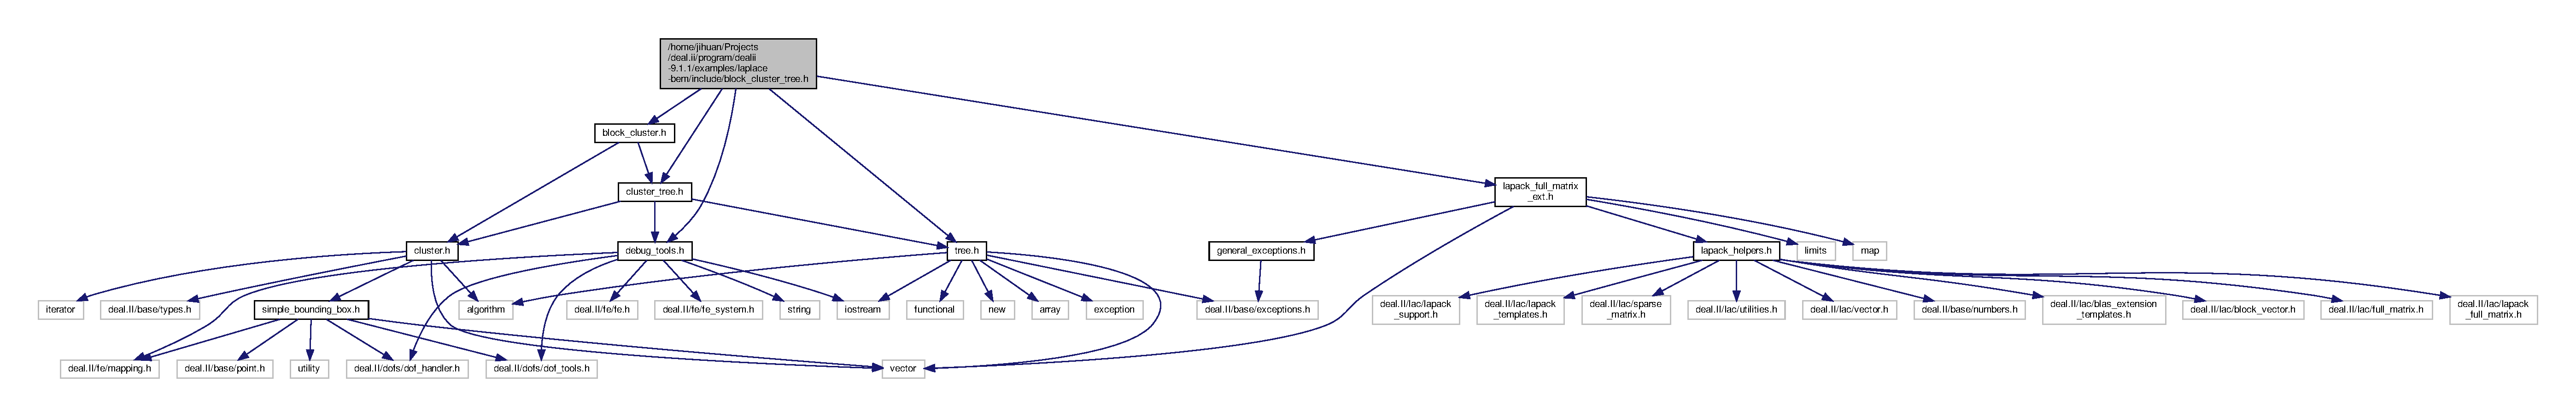
\includegraphics[width=350pt]{block__cluster__tree_8h__incl}
\end{center}
\end{figure}
This graph shows which files directly or indirectly include this file\+:\nopagebreak
\begin{figure}[H]
\begin{center}
\leavevmode

\includegraphics[width=350pt]{block__cluster__tree_8h__dep__incl}
\end{center}
\end{figure}
\subsection*{Classes}
\begin{DoxyCompactItemize}
\item 
class \hyperlink{classBlockClusterTree}{Block\+Cluster\+Tree$<$ spacedim, Number $>$}
\begin{DoxyCompactList}\small\item\em Class for block cluster tree. \end{DoxyCompactList}\end{DoxyCompactItemize}
\subsection*{Functions}
\textbf{ }\par
\begin{DoxyCompactItemize}
\item 
\mbox{\Hypertarget{block__cluster__tree_8h_a86a6c2e186f20eb650591ddca69940b7}\label{block__cluster__tree_8h_a86a6c2e186f20eb650591ddca69940b7}} 
{\footnotesize template$<$int spacedim, typename Number $>$ }\\std\+::ostream \& {\bfseries operator$<$$<$} (std\+::ostream \&out, const \hyperlink{classBlockClusterTree}{Block\+Cluster\+Tree}$<$ spacedim, Number $>$ \&block\+\_\+cluster\+\_\+tree)
\item 
{\footnotesize template$<$int spacedim, typename Number $>$ }\\void \hyperlink{block__cluster__tree_8h_a16ad2c7c8e746258ce244315d6181c72}{split\+\_\+block\+\_\+cluster\+\_\+node} (\hyperlink{classTreeNode}{Tree\+Node}$<$ \hyperlink{classBlockCluster}{Block\+Cluster}$<$ spacedim, Number $>$, \hyperlink{classBlockClusterTree}{Block\+Cluster\+Tree}$<$ spacedim, Number $>$\+::child\+\_\+num $>$ $\ast$bc\+\_\+node, \hyperlink{classBlockClusterTree}{Block\+Cluster\+Tree}$<$ spacedim, Number $>$ \&bc\+\_\+tree, const \hyperlink{tree_8h_a922ca07db9633957939f697a65aff11d}{Tree\+Node\+Split\+Mode} split\+\_\+mode, const bool if\+\_\+add\+\_\+child\+\_\+nodes\+\_\+to\+\_\+leaf\+\_\+set=true)
\item 
{\footnotesize template$<$int spacedim, typename Number  = double$>$ }\\bool \hyperlink{block__cluster__tree_8h_a3b2f90afbf0d192ac657f6fab5a87294}{prune\+\_\+to\+\_\+partition\+\_\+recursion} (\hyperlink{classBlockClusterTree}{Block\+Cluster\+Tree}$<$ spacedim, Number $>$ \&bct, const std\+::vector$<$ \hyperlink{classTreeNode}{Tree\+Node}$<$ \hyperlink{classBlockCluster}{Block\+Cluster}$<$ spacedim, Number $>$, \hyperlink{classBlockClusterTree}{Block\+Cluster\+Tree}$<$ spacedim, Number $>$\+::child\+\_\+num $>$ $\ast$$>$ \&partition, \hyperlink{classTreeNode}{Tree\+Node}$<$ \hyperlink{classBlockCluster}{Block\+Cluster}$<$ spacedim, Number $>$, \hyperlink{classBlockClusterTree}{Block\+Cluster\+Tree}$<$ spacedim, Number $>$\+::child\+\_\+num $>$ $\ast$bc\+\_\+node)
\item 
{\footnotesize template$<$int spacedim, typename Number $>$ }\\\hyperlink{classTreeNode}{Tree\+Node}$<$ \hyperlink{classBlockCluster}{Block\+Cluster}$<$ spacedim, Number $>$, \hyperlink{classBlockClusterTree}{Block\+Cluster\+Tree}$<$ spacedim, Number $>$\+::child\+\_\+num $>$ $\ast$ \hyperlink{block__cluster__tree_8h_a6ae11dfea883425641ebd2683cd482b6}{find\+\_\+bc\+\_\+node\+\_\+in\+\_\+partition\+\_\+intersect\+\_\+current\+\_\+bc\+\_\+node} (\hyperlink{classTreeNode}{Tree\+Node}$<$ \hyperlink{classBlockCluster}{Block\+Cluster}$<$ spacedim, Number $>$, \hyperlink{classBlockClusterTree}{Block\+Cluster\+Tree}$<$ spacedim, Number $>$\+::child\+\_\+num $>$ $\ast$current\+\_\+bc\+\_\+node, const std\+::vector$<$ \hyperlink{classTreeNode}{Tree\+Node}$<$ \hyperlink{classBlockCluster}{Block\+Cluster}$<$ spacedim, Number $>$, \hyperlink{classBlockClusterTree}{Block\+Cluster\+Tree}$<$ spacedim, Number $>$\+::child\+\_\+num $>$ $\ast$$>$ \&partition)
\item 
\mbox{\Hypertarget{block__cluster__tree_8h_a90e9fdffdd0ca85bd525dd9f29de3c93}\label{block__cluster__tree_8h_a90e9fdffdd0ca85bd525dd9f29de3c93}} 
{\footnotesize template$<$int spacedim, typename Number $>$ }\\\hyperlink{classTreeNode}{Tree\+Node}$<$ \hyperlink{classBlockCluster}{Block\+Cluster}$<$ spacedim, Number $>$, \hyperlink{classBlockClusterTree}{Block\+Cluster\+Tree}$<$ spacedim, Number $>$\+::child\+\_\+num $>$ $\ast$ {\bfseries find\+\_\+bc\+\_\+node\+\_\+in\+\_\+partition\+\_\+proper\+\_\+subset\+\_\+of\+\_\+current\+\_\+bc\+\_\+node} (\hyperlink{classTreeNode}{Tree\+Node}$<$ \hyperlink{classBlockCluster}{Block\+Cluster}$<$ spacedim, Number $>$, \hyperlink{classBlockClusterTree}{Block\+Cluster\+Tree}$<$ spacedim, Number $>$\+::child\+\_\+num $>$ $\ast$current\+\_\+bc\+\_\+node, const std\+::vector$<$ \hyperlink{classTreeNode}{Tree\+Node}$<$ \hyperlink{classBlockCluster}{Block\+Cluster}$<$ spacedim, Number $>$, \hyperlink{classBlockClusterTree}{Block\+Cluster\+Tree}$<$ spacedim, Number $>$\+::child\+\_\+num $>$ $\ast$$>$ \&partition)
\end{DoxyCompactItemize}



\subsection{Detailed Description}
Implementation of the class \hyperlink{classBlockClusterTree}{Block\+Cluster\+Tree}. 

\begin{DoxyDate}{Date}
2021-\/04-\/20 
\end{DoxyDate}
\begin{DoxyAuthor}{Author}
Jihuan Tian 
\end{DoxyAuthor}


\subsection{Function Documentation}
\mbox{\Hypertarget{block__cluster__tree_8h_a6ae11dfea883425641ebd2683cd482b6}\label{block__cluster__tree_8h_a6ae11dfea883425641ebd2683cd482b6}} 
\index{block\+\_\+cluster\+\_\+tree.\+h@{block\+\_\+cluster\+\_\+tree.\+h}!find\+\_\+bc\+\_\+node\+\_\+in\+\_\+partition\+\_\+intersect\+\_\+current\+\_\+bc\+\_\+node@{find\+\_\+bc\+\_\+node\+\_\+in\+\_\+partition\+\_\+intersect\+\_\+current\+\_\+bc\+\_\+node}}
\index{find\+\_\+bc\+\_\+node\+\_\+in\+\_\+partition\+\_\+intersect\+\_\+current\+\_\+bc\+\_\+node@{find\+\_\+bc\+\_\+node\+\_\+in\+\_\+partition\+\_\+intersect\+\_\+current\+\_\+bc\+\_\+node}!block\+\_\+cluster\+\_\+tree.\+h@{block\+\_\+cluster\+\_\+tree.\+h}}
\subsubsection{\texorpdfstring{find\+\_\+bc\+\_\+node\+\_\+in\+\_\+partition\+\_\+intersect\+\_\+current\+\_\+bc\+\_\+node()}{find\_bc\_node\_in\_partition\_intersect\_current\_bc\_node()}}
{\footnotesize\ttfamily template$<$int spacedim, typename Number $>$ \\
\hyperlink{classTreeNode}{Tree\+Node}$<$\hyperlink{classBlockCluster}{Block\+Cluster}$<$spacedim, Number$>$, \hyperlink{classBlockClusterTree}{Block\+Cluster\+Tree}$<$spacedim, Number$>$\+::child\+\_\+num$>$$\ast$ find\+\_\+bc\+\_\+node\+\_\+in\+\_\+partition\+\_\+intersect\+\_\+current\+\_\+bc\+\_\+node (\begin{DoxyParamCaption}\item[{\hyperlink{classTreeNode}{Tree\+Node}$<$ \hyperlink{classBlockCluster}{Block\+Cluster}$<$ spacedim, Number $>$, \hyperlink{classBlockClusterTree}{Block\+Cluster\+Tree}$<$ spacedim, Number $>$\+::child\+\_\+num $>$ $\ast$}]{current\+\_\+bc\+\_\+node,  }\item[{const std\+::vector$<$ \hyperlink{classTreeNode}{Tree\+Node}$<$ \hyperlink{classBlockCluster}{Block\+Cluster}$<$ spacedim, Number $>$, \hyperlink{classBlockClusterTree}{Block\+Cluster\+Tree}$<$ spacedim, Number $>$\+::child\+\_\+num $>$ $\ast$$>$ \&}]{partition }\end{DoxyParamCaption})}

Find a block cluster node in the given partition which has nonempty intersection with the current block cluster node. \begin{DoxyReturn}{Returns}

\end{DoxyReturn}


References Block\+Cluster\+Tree$<$ spacedim, Number $>$\+::partition().

\mbox{\Hypertarget{block__cluster__tree_8h_a3b2f90afbf0d192ac657f6fab5a87294}\label{block__cluster__tree_8h_a3b2f90afbf0d192ac657f6fab5a87294}} 
\index{block\+\_\+cluster\+\_\+tree.\+h@{block\+\_\+cluster\+\_\+tree.\+h}!prune\+\_\+to\+\_\+partition\+\_\+recursion@{prune\+\_\+to\+\_\+partition\+\_\+recursion}}
\index{prune\+\_\+to\+\_\+partition\+\_\+recursion@{prune\+\_\+to\+\_\+partition\+\_\+recursion}!block\+\_\+cluster\+\_\+tree.\+h@{block\+\_\+cluster\+\_\+tree.\+h}}
\subsubsection{\texorpdfstring{prune\+\_\+to\+\_\+partition\+\_\+recursion()}{prune\_to\_partition\_recursion()}}
{\footnotesize\ttfamily template$<$int spacedim, typename Number  = double$>$ \\
bool prune\+\_\+to\+\_\+partition\+\_\+recursion (\begin{DoxyParamCaption}\item[{\hyperlink{classBlockClusterTree}{Block\+Cluster\+Tree}$<$ spacedim, Number $>$ \&}]{bct,  }\item[{const std\+::vector$<$ \hyperlink{classTreeNode}{Tree\+Node}$<$ \hyperlink{classBlockCluster}{Block\+Cluster}$<$ spacedim, Number $>$, \hyperlink{classBlockClusterTree}{Block\+Cluster\+Tree}$<$ spacedim, Number $>$\+::child\+\_\+num $>$ $\ast$$>$ \&}]{partition,  }\item[{\hyperlink{classTreeNode}{Tree\+Node}$<$ \hyperlink{classBlockCluster}{Block\+Cluster}$<$ spacedim, Number $>$, \hyperlink{classBlockClusterTree}{Block\+Cluster\+Tree}$<$ spacedim, Number $>$\+::child\+\_\+num $>$ $\ast$}]{bc\+\_\+node }\end{DoxyParamCaption})}

Prune all those block cluster nodes which are descendants of the block cluster nodes specified in the given {\ttfamily partition}.


\begin{DoxyDescription}
\item[Note ]Because the block cluster nodes in the given {\ttfamily partition} are not contained in the block cluster tree, it is necessary to traverse the whole block cluster tree by recursion, during which each block cluster node is checked whether it belongs to the {\ttfamily partition} so that its descendants should be pruned. 
\end{DoxyDescription}


\begin{DoxyParams}{Parameters}
{\em bct} & The block cluster tree to be pruned. \\
\hline
{\em partition} & The given partition whose descendants will be pruned from the original block cluster tree. \\
\hline
{\em bc\+\_\+node} & The current block cluster node to be checked and determined whether it belongs to the partition so that its descendants should be pruned. \\
\hline
\end{DoxyParams}


References find\+\_\+pointer\+\_\+data(), Block\+Cluster\+Tree$<$ spacedim, Number $>$\+::partition(), and Block\+Cluster\+Tree$<$ spacedim, Number $>$\+::prune\+\_\+descendants\+\_\+from\+\_\+node().

\mbox{\Hypertarget{block__cluster__tree_8h_a16ad2c7c8e746258ce244315d6181c72}\label{block__cluster__tree_8h_a16ad2c7c8e746258ce244315d6181c72}} 
\index{block\+\_\+cluster\+\_\+tree.\+h@{block\+\_\+cluster\+\_\+tree.\+h}!split\+\_\+block\+\_\+cluster\+\_\+node@{split\+\_\+block\+\_\+cluster\+\_\+node}}
\index{split\+\_\+block\+\_\+cluster\+\_\+node@{split\+\_\+block\+\_\+cluster\+\_\+node}!block\+\_\+cluster\+\_\+tree.\+h@{block\+\_\+cluster\+\_\+tree.\+h}}
\subsubsection{\texorpdfstring{split\+\_\+block\+\_\+cluster\+\_\+node()}{split\_block\_cluster\_node()}}
{\footnotesize\ttfamily template$<$int spacedim, typename Number $>$ \\
void split\+\_\+block\+\_\+cluster\+\_\+node (\begin{DoxyParamCaption}\item[{\hyperlink{classTreeNode}{Tree\+Node}$<$ \hyperlink{classBlockCluster}{Block\+Cluster}$<$ spacedim, Number $>$, \hyperlink{classBlockClusterTree}{Block\+Cluster\+Tree}$<$ spacedim, Number $>$\+::child\+\_\+num $>$ $\ast$}]{bc\+\_\+node,  }\item[{\hyperlink{classBlockClusterTree}{Block\+Cluster\+Tree}$<$ spacedim, Number $>$ \&}]{bc\+\_\+tree,  }\item[{const \hyperlink{tree_8h_a922ca07db9633957939f697a65aff11d}{Tree\+Node\+Split\+Mode}}]{split\+\_\+mode,  }\item[{const bool}]{if\+\_\+add\+\_\+child\+\_\+nodes\+\_\+to\+\_\+leaf\+\_\+set = {\ttfamily true} }\end{DoxyParamCaption})}

Split a block cluster node in a block cluster tree according to the given split mode.

After the splitting, the total number of block cluster nodes in the block cluster tree will be updated. Whether the leaf set will be added with the newly created block cluster nodes is controlled by the flag {\ttfamily if\+\_\+add\+\_\+child\+\_\+nodes\+\_\+to\+\_\+leaf\+\_\+set}.


\begin{DoxyDescription}
\item[Note ]If the newly created block cluster nodes are to be added to the leaf set, their parent block cluster node should firstly be erased from the leaf set. This operation is not included in this function and should be performed beforehand. 
\end{DoxyDescription}


\begin{DoxyParams}{Parameters}
{\em bc\+\_\+node} & \\
\hline
{\em bc\+\_\+tree} & \\
\hline
{\em split\+\_\+mode} & \\
\hline
{\em if\+\_\+add\+\_\+child\+\_\+nodes\+\_\+to\+\_\+leaf\+\_\+set} & If the newly created block cluster nodes will be appended to the leaf set of the block cluster tree. \\
\hline
\end{DoxyParams}

\begin{DoxyDescription}
\item[Work flow ]


\begin{DoxyItemize}
\item Horizontal split mode 
\begin{DoxyEnumerate}
\item Set the split mode of the current block cluster node.


\item Create a new block cluster node by constructing its index set as $\tau^* \times \sigma$ with $\tau^* \in S(\tau)$. Its parent node is set to the current block cluster node.


\item Check if the block cluster node is small.


\item Append this new node as a child of the current block cluster node.


\item Add this new node to the leaf set if necessary.


\item Increase the total number of nodes in the block cluster tree.


\end{DoxyEnumerate}


\item Vertical split mode 
\begin{DoxyEnumerate}
\item Set the split mode of the current block cluster node.


\item Create a new block cluster node by constructing its index set as $\tau \times \sigma^*$ with $\sigma^* \in S(\sigma)$. Its parent node is set to the current block cluster node.


\item Check if the block cluster node is small.


\item Append this new node as a child of the current block cluster node.


\item Add this new node to the leaf set if necessary.


\item Increase the total number of nodes in the block cluster tree.


\end{DoxyEnumerate}


\item Cross split mode 
\begin{DoxyEnumerate}
\item Set the split mode of the current block cluster node.


\item Create a new block cluster node by constructing its index set as $\tau^* \times \sigma^*$ with $\tau^* \in S(\tau)$ and $\sigma^* \in S(\sigma)$. Its parent node is set to the current block cluster node.


\item Check if the block cluster node is small.


\item Append this new node as one of the children of the current block cluster node.


\item Add this new node to the leaf set if necessary.


\item Increase the total number of nodes in the block cluster tree.


\end{DoxyEnumerate}


\end{DoxyItemize}
\end{DoxyDescription}

Referenced by H\+Matrix$<$ spacedim, Number $>$\+::h\+\_\+h\+\_\+mmult\+\_\+cross\+\_\+split(), H\+Matrix$<$ spacedim, Number $>$\+::h\+\_\+h\+\_\+mmult\+\_\+horizontal\+\_\+split(), and H\+Matrix$<$ spacedim, Number $>$\+::h\+\_\+h\+\_\+mmult\+\_\+vertical\+\_\+split().


\hypertarget{cluster_8h}{}\section{/home/jihuan/\+Projects/deal.ii/program/dealii-\/9.1.1/examples/laplace-\/bem/include/cluster.h File Reference}
\label{cluster_8h}\index{/home/jihuan/\+Projects/deal.\+ii/program/dealii-\/9.\+1.\+1/examples/laplace-\/bem/include/cluster.\+h@{/home/jihuan/\+Projects/deal.\+ii/program/dealii-\/9.\+1.\+1/examples/laplace-\/bem/include/cluster.\+h}}


Implementation of the class \hyperlink{classCluster}{Cluster}.  


{\ttfamily \#include $<$deal.\+I\+I/base/types.\+h$>$}\newline
{\ttfamily \#include $<$algorithm$>$}\newline
{\ttfamily \#include $<$iterator$>$}\newline
{\ttfamily \#include $<$vector$>$}\newline
{\ttfamily \#include \char`\"{}simple\+\_\+bounding\+\_\+box.\+h\char`\"{}}\newline
Include dependency graph for cluster.\+h\+:\nopagebreak
\begin{figure}[H]
\begin{center}
\leavevmode
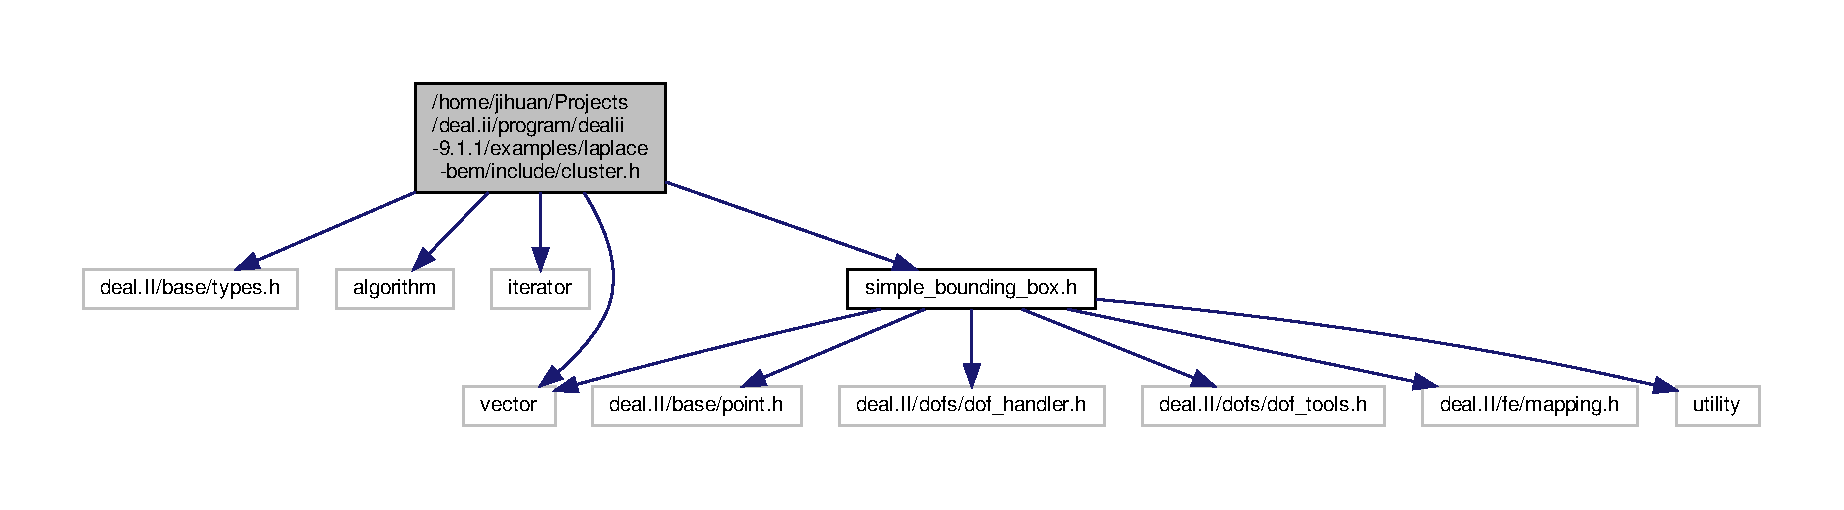
\includegraphics[width=350pt]{cluster_8h__incl}
\end{center}
\end{figure}
This graph shows which files directly or indirectly include this file\+:
\nopagebreak
\begin{figure}[H]
\begin{center}
\leavevmode

\includegraphics[width=350pt]{cluster_8h__dep__incl}
\end{center}
\end{figure}
\subsection*{Classes}
\begin{DoxyCompactItemize}
\item 
class \hyperlink{classCluster}{Cluster$<$ spacedim, Number $>$}
\begin{DoxyCompactList}\small\item\em Class for an index cluster. \end{DoxyCompactList}\end{DoxyCompactItemize}
\subsection*{Functions}
\textbf{ }\par
\begin{DoxyCompactItemize}
\item 
{\footnotesize template$<$int dim, int spacedim, typename Number  = double$>$ }\\void \hyperlink{group__hierarchical__matrices_gaeba0b2d80f64d0bb5c1ad86ac31bbcda}{map\+\_\+dofs\+\_\+to\+\_\+average\+\_\+cell\+\_\+size} (const Do\+F\+Handler$<$ dim, spacedim $>$ \&dof\+\_\+handler, std\+::vector$<$ Number $>$ \&dof\+\_\+average\+\_\+cell\+\_\+size)
\item 
{\footnotesize template$<$typename Do\+F\+Handler\+Type , typename Number  = double$>$ }\\void \hyperlink{group__hierarchical__matrices_ga1eee708f9eb5b9e9a2d8031c60c5d315}{map\+\_\+dofs\+\_\+to\+\_\+max\+\_\+cell\+\_\+size} (const Do\+F\+Handler\+Type \&dof\+\_\+handler, std\+::vector$<$ Number $>$ \&dof\+\_\+max\+\_\+cell\+\_\+size)
\item 
{\footnotesize template$<$typename Do\+F\+Handler\+Type , typename Number  = double$>$ }\\void \hyperlink{group__hierarchical__matrices_ga0a1c7de8480c4e9b4a002818f8c19b52}{map\+\_\+dofs\+\_\+to\+\_\+min\+\_\+cell\+\_\+size} (const Do\+F\+Handler\+Type \&dof\+\_\+handler, std\+::vector$<$ Number $>$ \&dof\+\_\+min\+\_\+cell\+\_\+size)
\item 
{\footnotesize template$<$int spacedim, typename Number $>$ }\\std\+::ostream \& \hyperlink{group__hierarchical__matrices_ga79f6d9af30209ae20bdf81906360664a}{operator$<$$<$} (std\+::ostream \&out, const \hyperlink{classCluster}{Cluster}$<$ spacedim, Number $>$ \&cluster)
\item 
{\footnotesize template$<$int spacedim, typename Number  = double$>$ }\\Number \hyperlink{group__hierarchical__matrices_gab6b0a51fb1b117f29902d220df72420a}{calc\+\_\+cluster\+\_\+distance} (const \hyperlink{classCluster}{Cluster}$<$ spacedim, Number $>$ \&cluster1, const \hyperlink{classCluster}{Cluster}$<$ spacedim, Number $>$ \&cluster2, const std\+::vector$<$ Point$<$ spacedim, Number $>$$>$ \&all\+\_\+support\+\_\+points)
\item 
{\footnotesize template$<$int spacedim, typename Number  = double$>$ }\\Number \hyperlink{group__hierarchical__matrices_ga76ef8db7b1a8500eac8d807bf104cacb}{calc\+\_\+cluster\+\_\+distance} (const \hyperlink{classCluster}{Cluster}$<$ spacedim, Number $>$ \&cluster1, const \hyperlink{classCluster}{Cluster}$<$ spacedim, Number $>$ \&cluster2, const std\+::vector$<$ Point$<$ spacedim, Number $>$$>$ \&all\+\_\+support\+\_\+points, const std\+::vector$<$ Number $>$ \&cell\+\_\+size\+\_\+at\+\_\+dofs)
\item 
{\footnotesize template$<$int spacedim, typename Number $>$ }\\bool {\bfseries operator==} (const \hyperlink{classCluster}{Cluster}$<$ spacedim, Number $>$ \&cluster1, const \hyperlink{classCluster}{Cluster}$<$ spacedim, Number $>$ \&cluster2)
\end{DoxyCompactItemize}



\subsection{Detailed Description}
Implementation of the class \hyperlink{classCluster}{Cluster}. 

\begin{DoxyDate}{Date}
2021-\/04-\/18 
\end{DoxyDate}
\begin{DoxyAuthor}{Author}
Jihuan Tian 
\end{DoxyAuthor}

\hypertarget{debug__tools_8h}{}\section{/home/jihuan/\+Projects/deal.ii/program/dealii-\/9.1.1/examples/laplace-\/bem/include/debug\+\_\+tools.h File Reference}
\label{debug__tools_8h}\index{/home/jihuan/\+Projects/deal.\+ii/program/dealii-\/9.\+1.\+1/examples/laplace-\/bem/include/debug\+\_\+tools.\+h@{/home/jihuan/\+Projects/deal.\+ii/program/dealii-\/9.\+1.\+1/examples/laplace-\/bem/include/debug\+\_\+tools.\+h}}


This file includes a bunch of helper functions for printing out and visualizing information about grid, Do\+Fs, map, etc.  


{\ttfamily \#include $<$deal.\+I\+I/dofs/dof\+\_\+handler.\+h$>$}\newline
{\ttfamily \#include $<$deal.\+I\+I/dofs/dof\+\_\+tools.\+h$>$}\newline
{\ttfamily \#include $<$deal.\+I\+I/fe/fe.\+h$>$}\newline
{\ttfamily \#include $<$deal.\+I\+I/fe/fe\+\_\+system.\+h$>$}\newline
{\ttfamily \#include $<$deal.\+I\+I/fe/mapping.\+h$>$}\newline
{\ttfamily \#include $<$iostream$>$}\newline
{\ttfamily \#include $<$string$>$}\newline
Include dependency graph for debug\+\_\+tools.\+h\+:\nopagebreak
\begin{figure}[H]
\begin{center}
\leavevmode
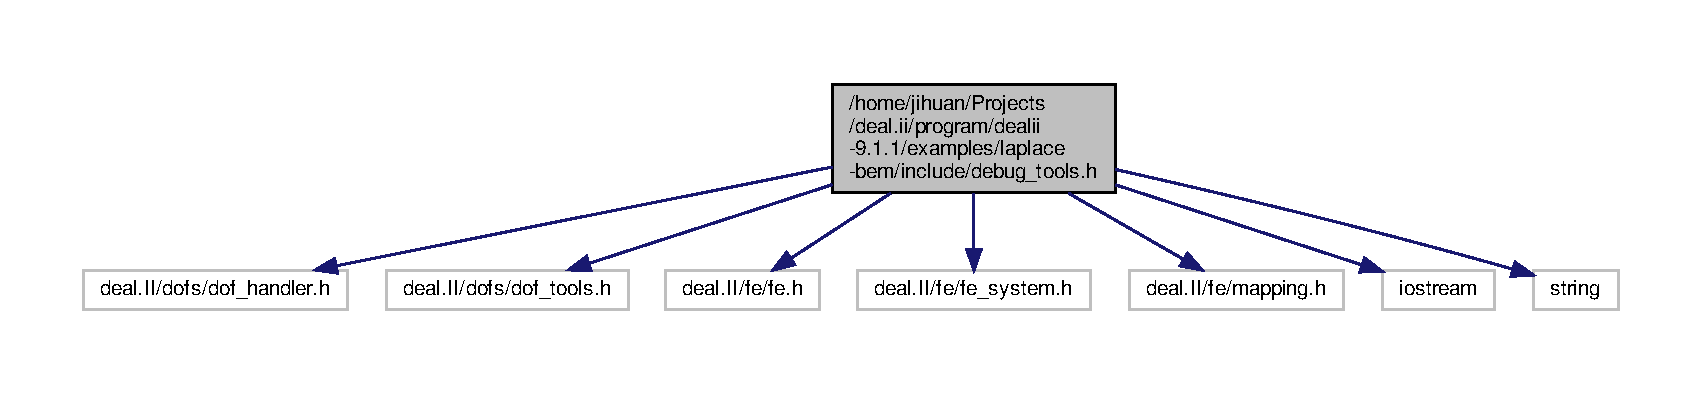
\includegraphics[width=350pt]{debug__tools_8h__incl}
\end{center}
\end{figure}
This graph shows which files directly or indirectly include this file\+:
\nopagebreak
\begin{figure}[H]
\begin{center}
\leavevmode
\includegraphics[width=350pt]{debug__tools_8h__dep__incl}
\end{center}
\end{figure}
\subsection*{Functions}
\begin{DoxyCompactItemize}
\item 
\mbox{\Hypertarget{debug__tools_8h_ad253b96a1f048532dc018fd4af3ff6e0}\label{debug__tools_8h_ad253b96a1f048532dc018fd4af3ff6e0}} 
{\footnotesize template$<$typename Vector\+Type $>$ }\\void {\bfseries print\+\_\+vector\+\_\+values} (std\+::ostream \&out, const Vector\+Type \&values, const std\+::string \&sep=std\+::string(\char`\"{},\char`\"{}), bool has\+\_\+newline=true)
\item 
\mbox{\Hypertarget{debug__tools_8h_a404e5fa4d0ac507edd6de3b59ff0714d}\label{debug__tools_8h_a404e5fa4d0ac507edd6de3b59ff0714d}} 
{\footnotesize template$<$typename Vector\+Type $>$ }\\void {\bfseries print\+\_\+vector\+\_\+indices} (std\+::ostream \&out, const Vector\+Type \&values, const std\+::string \&sep, bool index\+\_\+starting\+\_\+from\+\_\+zero, bool has\+\_\+newline=true)
\item 
\mbox{\Hypertarget{debug__tools_8h_af92377c94d59a332517fafeb5474c9dd}\label{debug__tools_8h_af92377c94d59a332517fafeb5474c9dd}} 
{\footnotesize template$<$typename Number $>$ }\\void {\bfseries print\+\_\+scalar\+\_\+to\+\_\+mat} (std\+::ostream \&out, const std\+::string \&name, const Number value)
\item 
\mbox{\Hypertarget{debug__tools_8h_a1398cb8a4f4a8e0f2384846df5b974ea}\label{debug__tools_8h_a1398cb8a4f4a8e0f2384846df5b974ea}} 
{\footnotesize template$<$typename Vector\+Type $>$ }\\void {\bfseries print\+\_\+vector\+\_\+to\+\_\+mat} (std\+::ostream \&out, const std\+::string \&name, const Vector\+Type \&values, bool is\+\_\+row\+\_\+vector=false)
\item 
\mbox{\Hypertarget{debug__tools_8h_a26839371749bbf1e0da9ac685f0a7dbf}\label{debug__tools_8h_a26839371749bbf1e0da9ac685f0a7dbf}} 
{\footnotesize template$<$typename Matrix\+Type $>$ }\\void {\bfseries print\+\_\+matrix\+\_\+to\+\_\+mat} (std\+::ostream \&out, const std\+::string \&name, const Matrix\+Type \&values, const unsigned int precision=8, const bool scientific=true, const unsigned int width=0, const char $\ast$zero\+\_\+string=\char`\"{}0\char`\"{}, const double denominator=1., const double threshold=0.)
\item 
\mbox{\Hypertarget{debug__tools_8h_a4c409b83d9b2d5772ec0fbfb4cb61cd5}\label{debug__tools_8h_a4c409b83d9b2d5772ec0fbfb4cb61cd5}} 
{\footnotesize template$<$typename node\+\_\+pointer\+\_\+type $>$ }\\void {\bfseries print\+\_\+vector\+\_\+of\+\_\+tree\+\_\+node\+\_\+pointer\+\_\+values} (std\+::ostream \&out, const std\+::vector$<$ node\+\_\+pointer\+\_\+type $>$ \&tree\+\_\+node\+\_\+pointers, const std\+::string \&sep=std\+::string(\char`\"{},\char`\"{}))
\item 
{\footnotesize template$<$int dim, int spacedim$>$ }\\void \hyperlink{debug__tools_8h_a864e453be7ec58dd6e9ceb48e14e750c}{print\+\_\+support\+\_\+point\+\_\+info} (const Finite\+Element$<$ dim, spacedim $>$ \&fe, const Mapping$<$ dim, spacedim $>$ \&mapping, const Do\+F\+Handler$<$ dim, spacedim $>$ \&dof\+\_\+handler, const std\+::string \&base\+\_\+name)
\begin{DoxyCompactList}\small\item\em Generate a table of DoF indices associated with each support point. \end{DoxyCompactList}\item 
{\footnotesize template$<$int dim, int spacedim$>$ }\\void \hyperlink{debug__tools_8h_aed4a1a4736bce80ce849cc0dfa9a7616}{print\+\_\+support\+\_\+point\+\_\+info} (const F\+E\+System$<$ dim, spacedim $>$ \&fe\+\_\+system, const Mapping$<$ dim, spacedim $>$ \&mapping, const Do\+F\+Handler$<$ dim, spacedim $>$ \&dof\+\_\+handler, const std\+::string \&base\+\_\+name)
\begin{DoxyCompactList}\small\item\em Generate a table of DoF indices associated with each support point. \end{DoxyCompactList}\end{DoxyCompactItemize}


\subsection{Detailed Description}
This file includes a bunch of helper functions for printing out and visualizing information about grid, Do\+Fs, map, etc. 

\begin{DoxyDate}{Date}
2021-\/04-\/25 
\end{DoxyDate}
\begin{DoxyAuthor}{Author}
Jihuan Tian 
\end{DoxyAuthor}


\subsection{Function Documentation}
\mbox{\Hypertarget{debug__tools_8h_a864e453be7ec58dd6e9ceb48e14e750c}\label{debug__tools_8h_a864e453be7ec58dd6e9ceb48e14e750c}} 
\index{debug\+\_\+tools.\+h@{debug\+\_\+tools.\+h}!print\+\_\+support\+\_\+point\+\_\+info@{print\+\_\+support\+\_\+point\+\_\+info}}
\index{print\+\_\+support\+\_\+point\+\_\+info@{print\+\_\+support\+\_\+point\+\_\+info}!debug\+\_\+tools.\+h@{debug\+\_\+tools.\+h}}
\subsubsection{\texorpdfstring{print\+\_\+support\+\_\+point\+\_\+info()}{print\_support\_point\_info()}\hspace{0.1cm}{\footnotesize\ttfamily [1/2]}}
{\footnotesize\ttfamily template$<$int dim, int spacedim$>$ \\
void print\+\_\+support\+\_\+point\+\_\+info (\begin{DoxyParamCaption}\item[{const Finite\+Element$<$ dim, spacedim $>$ \&}]{fe,  }\item[{const Mapping$<$ dim, spacedim $>$ \&}]{mapping,  }\item[{const Do\+F\+Handler$<$ dim, spacedim $>$ \&}]{dof\+\_\+handler,  }\item[{const std\+::string \&}]{base\+\_\+name }\end{DoxyParamCaption})}



Generate a table of DoF indices associated with each support point. 

The information in the table is defined in the given Mapping and Do\+F\+Handler objects, which can be then visualized in Gnuplot by executing the following command.
\begin{DoxyEnumerate}
\item For spacedim=2\+: 
\begin{DoxyCode}
plot \textcolor{stringliteral}{"./data\_file.gpl"} \textcolor{keyword}{using} 1:2:3 with labels offset 1,1 point pt 1 lc rgb \(\backslash\)
\textcolor{stringliteral}{"red"} notitle
\end{DoxyCode}

\item For spacedim=3\+: 
\begin{DoxyCode}
splot \textcolor{stringliteral}{"./data\_file.gpl"} \textcolor{keyword}{using} 1:2:3:4 with labels offset 1,1 point pt 1 lc \(\backslash\)
rgb \textcolor{stringliteral}{"red"}
\end{DoxyCode}
 
\begin{DoxyParams}{Parameters}
{\em fe\+\_\+system} & The given Finite\+Element object will be checked if it has support points. \\
\hline
{\em mapping} & \\
\hline
{\em dof\+\_\+handler} & \\
\hline
{\em base\+\_\+name} & \\
\hline
\end{DoxyParams}

\end{DoxyEnumerate}Allocate memory for the vector storing support points.

Get the list of support point coordinates for all Do\+Fs. The Do\+Fs are in the default numbering starting from 0.

Write the table of DoF indices for each support point into file.

Referenced by main().

\mbox{\Hypertarget{debug__tools_8h_aed4a1a4736bce80ce849cc0dfa9a7616}\label{debug__tools_8h_aed4a1a4736bce80ce849cc0dfa9a7616}} 
\index{debug\+\_\+tools.\+h@{debug\+\_\+tools.\+h}!print\+\_\+support\+\_\+point\+\_\+info@{print\+\_\+support\+\_\+point\+\_\+info}}
\index{print\+\_\+support\+\_\+point\+\_\+info@{print\+\_\+support\+\_\+point\+\_\+info}!debug\+\_\+tools.\+h@{debug\+\_\+tools.\+h}}
\subsubsection{\texorpdfstring{print\+\_\+support\+\_\+point\+\_\+info()}{print\_support\_point\_info()}\hspace{0.1cm}{\footnotesize\ttfamily [2/2]}}
{\footnotesize\ttfamily template$<$int dim, int spacedim$>$ \\
void print\+\_\+support\+\_\+point\+\_\+info (\begin{DoxyParamCaption}\item[{const F\+E\+System$<$ dim, spacedim $>$ \&}]{fe\+\_\+system,  }\item[{const Mapping$<$ dim, spacedim $>$ \&}]{mapping,  }\item[{const Do\+F\+Handler$<$ dim, spacedim $>$ \&}]{dof\+\_\+handler,  }\item[{const std\+::string \&}]{base\+\_\+name }\end{DoxyParamCaption})}



Generate a table of DoF indices associated with each support point. 

The information in the table is defined in the given Mapping and Do\+F\+Handler objects, which can be then visualized in Gnuplot by executing the following command.
\begin{DoxyEnumerate}
\item For spacedim=2\+: 
\begin{DoxyCode}
plot \textcolor{stringliteral}{"./data\_file.gpl"} \textcolor{keyword}{using} 1:2:3 with labels offset 1,1 point pt 1 lc rgb \(\backslash\)
\textcolor{stringliteral}{"red"} notitle
\end{DoxyCode}

\item For spacedim=3\+: 
\begin{DoxyCode}
splot \textcolor{stringliteral}{"./data\_file.gpl"} \textcolor{keyword}{using} 1:2:3:4 with labels offset 1,1 point pt 1 lc \(\backslash\)
rgb \textcolor{stringliteral}{"red"}
\end{DoxyCode}
 
\begin{DoxyParams}{Parameters}
{\em fe\+\_\+system} & The given F\+E\+System object will be checked if it has support points. \\
\hline
{\em mapping} & \\
\hline
{\em dof\+\_\+handler} & \\
\hline
{\em base\+\_\+name} & \\
\hline
\end{DoxyParams}

\end{DoxyEnumerate}Allocate memory for the vector storing support points.

Get the list of support point coordinates for all Do\+Fs. The Do\+Fs are in the default numbering starting from 0.

Write the table of DoF indices for each support point into file.
\hypertarget{general__exceptions_8h}{}\section{/home/jihuan/\+Projects/deal.ii/program/dealii-\/9.1.1/examples/laplace-\/bem/include/general\+\_\+exceptions.h File Reference}
\label{general__exceptions_8h}\index{/home/jihuan/\+Projects/deal.\+ii/program/dealii-\/9.\+1.\+1/examples/laplace-\/bem/include/general\+\_\+exceptions.\+h@{/home/jihuan/\+Projects/deal.\+ii/program/dealii-\/9.\+1.\+1/examples/laplace-\/bem/include/general\+\_\+exceptions.\+h}}


Definition of self-\/defined general exceptions.  


{\ttfamily \#include $<$deal.\+I\+I/base/exceptions.\+h$>$}\newline
Include dependency graph for general\+\_\+exceptions.\+h\+:\nopagebreak
\begin{figure}[H]
\begin{center}
\leavevmode
\includegraphics[width=247pt]{general__exceptions_8h__incl}
\end{center}
\end{figure}
This graph shows which files directly or indirectly include this file\+:
\nopagebreak
\begin{figure}[H]
\begin{center}
\leavevmode
\includegraphics[width=350pt]{general__exceptions_8h__dep__incl}
\end{center}
\end{figure}
\subsection*{Functions}
\begin{DoxyCompactItemize}
\item 
\mbox{\Hypertarget{general__exceptions_8h_a1c69f2e31438caa9d94728d2bbc9a3ec}\label{general__exceptions_8h_a1c69f2e31438caa9d94728d2bbc9a3ec}} 
{\bfseries Decl\+Exception3} (Exc\+Open\+Interval\+Range, double, double, double,$<$$<$ arg1$<$$<$ \char`\"{} is not in the range (\char`\"{}$<$$<$ arg2$<$$<$ \char`\"{}, \char`\"{}$<$$<$ arg3$<$$<$ \char`\"{}).\char`\"{})
\item 
\mbox{\Hypertarget{general__exceptions_8h_a6a4365f3bbd7f17fe9ba09f06b0fbe12}\label{general__exceptions_8h_a6a4365f3bbd7f17fe9ba09f06b0fbe12}} 
{\bfseries Decl\+Exception3} (Exc\+Left\+Open\+Interval\+Range, double, double, double,$<$$<$ arg1$<$$<$ \char`\"{} is not in the range (\char`\"{}$<$$<$ arg2$<$$<$ \char`\"{}, \char`\"{}$<$$<$ arg3$<$$<$ \char`\"{}\mbox{]}.\char`\"{})
\item 
\mbox{\Hypertarget{general__exceptions_8h_a17fb3746741a79d90a8b4b11d82fc162}\label{general__exceptions_8h_a17fb3746741a79d90a8b4b11d82fc162}} 
{\bfseries Decl\+Exception3} (Exc\+Right\+Open\+Interval\+Range, double, double, double,$<$$<$ arg1$<$$<$ \char`\"{} is not in the range \mbox{[}\char`\"{}$<$$<$ arg2$<$$<$ \char`\"{}, \char`\"{}$<$$<$ arg3$<$$<$ \char`\"{}).\char`\"{})
\item 
\mbox{\Hypertarget{general__exceptions_8h_a5b046d9de002841c9c2acbd6928bb68b}\label{general__exceptions_8h_a5b046d9de002841c9c2acbd6928bb68b}} 
{\bfseries Decl\+Exception3} (Exc\+Closed\+Interval\+Range, double, double, double,$<$$<$ arg1$<$$<$ \char`\"{} is not in the range \mbox{[}\char`\"{}$<$$<$ arg2$<$$<$ \char`\"{}, \char`\"{}$<$$<$ arg3$<$$<$ \char`\"{}\mbox{]}.\char`\"{})
\end{DoxyCompactItemize}


\subsection{Detailed Description}
Definition of self-\/defined general exceptions. 

\begin{DoxyDate}{Date}
2021-\/06-\/10 
\end{DoxyDate}
\begin{DoxyAuthor}{Author}
Jihuan Tian 
\end{DoxyAuthor}

\hypertarget{generic__functors_8h}{}\section{/home/jihuan/\+Projects/deal.ii/program/dealii-\/9.1.1/examples/laplace-\/bem/include/generic\+\_\+functors.h File Reference}
\label{generic__functors_8h}\index{/home/jihuan/\+Projects/deal.\+ii/program/dealii-\/9.\+1.\+1/examples/laplace-\/bem/include/generic\+\_\+functors.\+h@{/home/jihuan/\+Projects/deal.\+ii/program/dealii-\/9.\+1.\+1/examples/laplace-\/bem/include/generic\+\_\+functors.\+h}}


This header file contains a set of self-\/defined generic functors.  


{\ttfamily \#include $<$deal.\+I\+I/base/types.\+h$>$}\newline
{\ttfamily \#include $<$map$>$}\newline
{\ttfamily \#include $<$vector$>$}\newline
Include dependency graph for generic\+\_\+functors.\+h\+:\nopagebreak
\begin{figure}[H]
\begin{center}
\leavevmode
\includegraphics[width=299pt]{generic__functors_8h__incl}
\end{center}
\end{figure}
This graph shows which files directly or indirectly include this file\+:\nopagebreak
\begin{figure}[H]
\begin{center}
\leavevmode
\includegraphics[width=350pt]{generic__functors_8h__dep__incl}
\end{center}
\end{figure}
\subsection*{Functions}
\begin{DoxyCompactItemize}
\item 
{\footnotesize template$<$typename Input\+Iterator , typename T $>$ }\\Input\+Iterator \hyperlink{generic__functors_8h_ad741e5fc6f9f2d7acafe6e5530b1f52e}{find\+\_\+pointer\+\_\+data} (Input\+Iterator first, Input\+Iterator last, const T $\ast$value\+\_\+pointer)
\item 
void \hyperlink{generic__functors_8h_a45ed12a09686ebca5400b5161a186c09}{build\+\_\+index\+\_\+set\+\_\+global\+\_\+to\+\_\+local\+\_\+map} (const std\+::vector$<$ dealii\+::types\+::global\+\_\+dof\+\_\+index $>$ \&index\+\_\+set\+\_\+as\+\_\+local\+\_\+to\+\_\+global\+\_\+map, std\+::map$<$ dealii\+::types\+::global\+\_\+dof\+\_\+index, size\+\_\+t $>$ \&global\+\_\+to\+\_\+local\+\_\+map)
\end{DoxyCompactItemize}


\subsection{Detailed Description}
This header file contains a set of self-\/defined generic functors. 

\begin{DoxyDate}{Date}
2021-\/07-\/20 
\end{DoxyDate}
\begin{DoxyAuthor}{Author}
Jihuan Tian 
\end{DoxyAuthor}


\subsection{Function Documentation}
\mbox{\Hypertarget{generic__functors_8h_a45ed12a09686ebca5400b5161a186c09}\label{generic__functors_8h_a45ed12a09686ebca5400b5161a186c09}} 
\index{generic\+\_\+functors.\+h@{generic\+\_\+functors.\+h}!build\+\_\+index\+\_\+set\+\_\+global\+\_\+to\+\_\+local\+\_\+map@{build\+\_\+index\+\_\+set\+\_\+global\+\_\+to\+\_\+local\+\_\+map}}
\index{build\+\_\+index\+\_\+set\+\_\+global\+\_\+to\+\_\+local\+\_\+map@{build\+\_\+index\+\_\+set\+\_\+global\+\_\+to\+\_\+local\+\_\+map}!generic\+\_\+functors.\+h@{generic\+\_\+functors.\+h}}
\subsubsection{\texorpdfstring{build\+\_\+index\+\_\+set\+\_\+global\+\_\+to\+\_\+local\+\_\+map()}{build\_index\_set\_global\_to\_local\_map()}}
{\footnotesize\ttfamily void build\+\_\+index\+\_\+set\+\_\+global\+\_\+to\+\_\+local\+\_\+map (\begin{DoxyParamCaption}\item[{const std\+::vector$<$ dealii\+::types\+::global\+\_\+dof\+\_\+index $>$ \&}]{index\+\_\+set\+\_\+as\+\_\+local\+\_\+to\+\_\+global\+\_\+map,  }\item[{std\+::map$<$ dealii\+::types\+::global\+\_\+dof\+\_\+index, size\+\_\+t $>$ \&}]{global\+\_\+to\+\_\+local\+\_\+map }\end{DoxyParamCaption})}

Build a map from global indices to local indices based on the given index set, which is actually a map from local indices to global indices. 
\begin{DoxyParams}{Parameters}
{\em index\+\_\+set\+\_\+as\+\_\+local\+\_\+to\+\_\+global\+\_\+map} & \\
\hline
{\em global\+\_\+to\+\_\+local\+\_\+map} & \\
\hline
\end{DoxyParams}


Referenced by convert\+H\+Mat\+Block\+To\+Rk\+Matrix(), f\+\_\+h\+\_\+mmult(), find\+\_\+pointer\+\_\+data(), h\+\_\+f\+\_\+mmult(), h\+\_\+rk\+\_\+mmult(), Init\+And\+Create\+H\+Matrix\+Children(), main(), and rk\+\_\+h\+\_\+mmult().

\mbox{\Hypertarget{generic__functors_8h_ad741e5fc6f9f2d7acafe6e5530b1f52e}\label{generic__functors_8h_ad741e5fc6f9f2d7acafe6e5530b1f52e}} 
\index{generic\+\_\+functors.\+h@{generic\+\_\+functors.\+h}!find\+\_\+pointer\+\_\+data@{find\+\_\+pointer\+\_\+data}}
\index{find\+\_\+pointer\+\_\+data@{find\+\_\+pointer\+\_\+data}!generic\+\_\+functors.\+h@{generic\+\_\+functors.\+h}}
\subsubsection{\texorpdfstring{find\+\_\+pointer\+\_\+data()}{find\_pointer\_data()}}
{\footnotesize\ttfamily template$<$typename Input\+Iterator , typename T $>$ \\
Input\+Iterator find\+\_\+pointer\+\_\+data (\begin{DoxyParamCaption}\item[{Input\+Iterator}]{first,  }\item[{Input\+Iterator}]{last,  }\item[{const T $\ast$}]{value\+\_\+pointer }\end{DoxyParamCaption})}

Find the pointer in a list of pointers of the same type. The comparison is based on the data being pointed instead of the pointer addresses. 
\begin{DoxyParams}{Parameters}
{\em first} & \\
\hline
{\em last} & \\
\hline
{\em value\+\_\+pointer} & \\
\hline
\end{DoxyParams}
\begin{DoxyReturn}{Returns}

\end{DoxyReturn}
N.\+B. Here we use {\ttfamily }($\ast$first) to get the pointer stored in the container. Then use ($\ast$($\ast$first)) to get the data associated with this pointer.

References build\+\_\+index\+\_\+set\+\_\+global\+\_\+to\+\_\+local\+\_\+map().



Referenced by H\+Matrix$<$ spacedim, Number $>$\+::coarsen\+\_\+to\+\_\+partition(), and prune\+\_\+to\+\_\+partition\+\_\+recursion().


\hypertarget{hmatrix_8h}{}\section{/home/jihuan/\+Projects/deal.ii/program/dealii-\/9.1.1/examples/laplace-\/bem/include/hmatrix.h File Reference}
\label{hmatrix_8h}\index{/home/jihuan/\+Projects/deal.\+ii/program/dealii-\/9.\+1.\+1/examples/laplace-\/bem/include/hmatrix.\+h@{/home/jihuan/\+Projects/deal.\+ii/program/dealii-\/9.\+1.\+1/examples/laplace-\/bem/include/hmatrix.\+h}}


Definition of hierarchical matrix.  


{\ttfamily \#include $<$deal.\+I\+I/base/logstream.\+h$>$}\newline
{\ttfamily \#include $<$deal.\+I\+I/lac/full\+\_\+matrix.\+h$>$}\newline
{\ttfamily \#include $<$algorithm$>$}\newline
{\ttfamily \#include $<$fstream$>$}\newline
{\ttfamily \#include $<$iostream$>$}\newline
{\ttfamily \#include $<$map$>$}\newline
{\ttfamily \#include $<$string$>$}\newline
{\ttfamily \#include $<$utility$>$}\newline
{\ttfamily \#include $<$vector$>$}\newline
{\ttfamily \#include \char`\"{}block\+\_\+cluster.\+h\char`\"{}}\newline
{\ttfamily \#include \char`\"{}block\+\_\+cluster\+\_\+tree.\+h\char`\"{}}\newline
{\ttfamily \#include \char`\"{}generic\+\_\+functors.\+h\char`\"{}}\newline
{\ttfamily \#include \char`\"{}lapack\+\_\+full\+\_\+matrix\+\_\+ext.\+h\char`\"{}}\newline
{\ttfamily \#include \char`\"{}rkmatrix.\+h\char`\"{}}\newline
Include dependency graph for hmatrix.\+h\+:\nopagebreak
\begin{figure}[H]
\begin{center}
\leavevmode
\includegraphics[width=350pt]{hmatrix_8h__incl}
\end{center}
\end{figure}
This graph shows which files directly or indirectly include this file\+:\nopagebreak
\begin{figure}[H]
\begin{center}
\leavevmode
\includegraphics[width=350pt]{hmatrix_8h__dep__incl}
\end{center}
\end{figure}
\subsection*{Classes}
\begin{DoxyCompactItemize}
\item 
class \hyperlink{classHMatrix}{H\+Matrix$<$ spacedim, Number $>$}
\end{DoxyCompactItemize}
\subsection*{Enumerations}
\begin{DoxyCompactItemize}
\item 
enum \hyperlink{hmatrix_8h_ac04719e202c88f36e4533fe1d326a494}{H\+Matrix\+Type} \{ \hyperlink{hmatrix_8h_ac04719e202c88f36e4533fe1d326a494a51de26f7a73c478c006090ae907e7924}{Full\+Matrix\+Type}, 
\hyperlink{hmatrix_8h_ac04719e202c88f36e4533fe1d326a494a2cf6ea273987e941519349b7c4b0b88c}{Rk\+Matrix\+Type}, 
\hyperlink{hmatrix_8h_ac04719e202c88f36e4533fe1d326a494a8721e6353d7dcebee5c58f4990a0241d}{Hierarchical\+Matrix\+Type}, 
\hyperlink{hmatrix_8h_ac04719e202c88f36e4533fe1d326a494aba1ff44c7102f5c03299dffd067b74b7}{Undefined\+Matrix\+Type}
 \}
\end{DoxyCompactItemize}
\subsection*{Functions}
\begin{DoxyCompactItemize}
\item 
\mbox{\Hypertarget{hmatrix_8h_a42e2d29cc860fddf6697fc294d76460a}\label{hmatrix_8h_a42e2d29cc860fddf6697fc294d76460a}} 
{\bfseries Decl\+Exception1} (Exc\+Invalid\+H\+Matrix\+Type, \hyperlink{hmatrix_8h_ac04719e202c88f36e4533fe1d326a494}{H\+Matrix\+Type},$<$$<$ \char`\"{}Invalid \hyperlink{classHMatrix}{H\+Matrix} type \char`\"{}$<$$<$ arg1)
\item 
{\footnotesize template$<$int spacedim, typename Number  = double$>$ }\\void \hyperlink{hmatrix_8h_a21892e360616f81dd5ad1c7089f9eaab}{Init\+H\+Matrix\+Wrt\+Block\+Cluster\+Node} (\hyperlink{classHMatrix}{H\+Matrix}$<$ spacedim, Number $>$ \&hmat, typename \hyperlink{classBlockClusterTree}{Block\+Cluster\+Tree}$<$ spacedim, Number $>$\+::node\+\_\+const\+\_\+pointer\+\_\+type bc\+\_\+node)
\item 
{\footnotesize template$<$int spacedim, typename Number  = double$>$ }\\void \hyperlink{hmatrix_8h_ae5d510b10595b78a40764950441bcbaf}{Init\+H\+Matrix\+Wrt\+Block\+Cluster\+Node} (\hyperlink{classHMatrix}{H\+Matrix}$<$ spacedim, Number $>$ \&hmat, typename \hyperlink{classBlockClusterTree}{Block\+Cluster\+Tree}$<$ spacedim, Number $>$\+::node\+\_\+const\+\_\+pointer\+\_\+type bc\+\_\+node, const std\+::vector$<$ std\+::pair$<$ \hyperlink{classHMatrix}{H\+Matrix}$<$ spacedim, Number $>$ $\ast$, \hyperlink{classHMatrix}{H\+Matrix}$<$ spacedim, Number $>$ $\ast$$>$$>$ \&Sigma\+\_\+P)
\item 
{\footnotesize template$<$int spacedim, typename Number  = double$>$ }\\void \hyperlink{hmatrix_8h_a0f1d1afba43d1a66f46ee4799a9904a2}{Init\+H\+Matrix\+Wrt\+Block\+Cluster\+Node} (\hyperlink{classHMatrix}{H\+Matrix}$<$ spacedim, Number $>$ \&hmat, typename \hyperlink{classBlockClusterTree}{Block\+Cluster\+Tree}$<$ spacedim, Number $>$\+::node\+\_\+const\+\_\+pointer\+\_\+type bc\+\_\+node, const std\+::pair$<$ \hyperlink{classHMatrix}{H\+Matrix}$<$ spacedim, Number $>$ $\ast$, \hyperlink{classHMatrix}{H\+Matrix}$<$ spacedim, Number $>$ $\ast$$>$ \&hmat\+\_\+pair)
\item 
{\footnotesize template$<$int spacedim, typename Number  = double$>$ }\\void \hyperlink{hmatrix_8h_a317e4841d6bb5b60883a7e21027a8893}{Init\+And\+Create\+H\+Matrix\+Children} (\hyperlink{classHMatrix}{H\+Matrix}$<$ spacedim, Number $>$ $\ast$hmat, typename \hyperlink{classBlockClusterTree}{Block\+Cluster\+Tree}$<$ spacedim, Number $>$\+::node\+\_\+const\+\_\+pointer\+\_\+type bc\+\_\+node, const unsigned int fixed\+\_\+rank\+\_\+k, bool is\+\_\+build\+\_\+index\+\_\+set\+\_\+global\+\_\+to\+\_\+local\+\_\+map=true)
\item 
{\footnotesize template$<$int spacedim, typename Number  = double$>$ }\\void \hyperlink{hmatrix_8h_a2b56a9e943f5632f50d08f4e892b1787}{Init\+And\+Create\+H\+Matrix\+Children} (\hyperlink{classHMatrix}{H\+Matrix}$<$ spacedim, Number $>$ $\ast$hmat, typename \hyperlink{classBlockClusterTree}{Block\+Cluster\+Tree}$<$ spacedim, Number $>$\+::node\+\_\+const\+\_\+pointer\+\_\+type bc\+\_\+node, const unsigned int fixed\+\_\+rank\+\_\+k, const \hyperlink{classLAPACKFullMatrixExt}{L\+A\+P\+A\+C\+K\+Full\+Matrix\+Ext}$<$ Number $>$ \&M, bool is\+\_\+build\+\_\+index\+\_\+set\+\_\+global\+\_\+to\+\_\+local\+\_\+map=true)
\item 
{\footnotesize template$<$int spacedim, typename Number  = double$>$ }\\void \hyperlink{hmatrix_8h_a53120559ced904c076a4914af3e9423a}{Init\+And\+Create\+H\+Matrix\+Children} (\hyperlink{classHMatrix}{H\+Matrix}$<$ spacedim, Number $>$ $\ast$hmat, typename \hyperlink{classBlockClusterTree}{Block\+Cluster\+Tree}$<$ spacedim, Number $>$\+::node\+\_\+const\+\_\+pointer\+\_\+type bc\+\_\+node, const unsigned int fixed\+\_\+rank\+\_\+k, const \hyperlink{classLAPACKFullMatrixExt}{L\+A\+P\+A\+C\+K\+Full\+Matrix\+Ext}$<$ Number $>$ \&M, const std\+::map$<$ types\+::global\+\_\+dof\+\_\+index, size\+\_\+t $>$ \&row\+\_\+index\+\_\+global\+\_\+to\+\_\+local\+\_\+map\+\_\+for\+\_\+M, const std\+::map$<$ types\+::global\+\_\+dof\+\_\+index, size\+\_\+t $>$ \&col\+\_\+index\+\_\+global\+\_\+to\+\_\+local\+\_\+map\+\_\+for\+\_\+M, bool is\+\_\+build\+\_\+index\+\_\+set\+\_\+global\+\_\+to\+\_\+local\+\_\+map=true)
\item 
{\footnotesize template$<$int spacedim, typename Number  = double$>$ }\\void \hyperlink{hmatrix_8h_a9cf5008e3967b1029d5b766290c98139}{Init\+And\+Create\+H\+Matrix\+Children} (\hyperlink{classHMatrix}{H\+Matrix}$<$ spacedim, Number $>$ $\ast$hmat, typename \hyperlink{classBlockClusterTree}{Block\+Cluster\+Tree}$<$ spacedim, Number $>$\+::node\+\_\+const\+\_\+pointer\+\_\+type bc\+\_\+node, \hyperlink{classHMatrix}{H\+Matrix}$<$ spacedim, Number $>$ \&\&H)
\item 
{\footnotesize template$<$int spacedim, typename Number $>$ }\\void \hyperlink{hmatrix_8h_a090df12c1646d637bc390fa6dae55f24}{Refine\+H\+Matrix\+Wrt\+Extended\+Block\+Cluster\+Tree} (\hyperlink{classHMatrix}{H\+Matrix}$<$ spacedim, Number $>$ $\ast$starting\+\_\+hmat, \hyperlink{classHMatrix}{H\+Matrix}$<$ spacedim, Number $>$ $\ast$current\+\_\+hmat)
\item 
{\footnotesize template$<$int spacedim, typename Number  = double$>$ }\\void \hyperlink{hmatrix_8h_a13b0f4d71b52952d99ee7ecb0eb033cb}{convert\+H\+Mat\+Block\+To\+Rk\+Matrix} (\hyperlink{classHMatrix}{H\+Matrix}$<$ spacedim, Number $>$ $\ast$hmat\+\_\+block, const unsigned int fixed\+\_\+rank\+\_\+k, const \hyperlink{classHMatrix}{H\+Matrix}$<$ spacedim, Number $>$ $\ast$hmat\+\_\+root\+\_\+block=nullptr, size\+\_\+t $\ast$calling\+\_\+counter=nullptr, const std\+::string \&output\+\_\+file\+\_\+base\+\_\+name=std\+::string(\char`\"{}hmat-\/bct\char`\"{}))
\item 
{\footnotesize template$<$int spacedim, typename Number  = double$>$ }\\void \hyperlink{hmatrix_8h_afee9050ba0b224929bcbf99484385a59}{h\+\_\+rk\+\_\+mmult} (\hyperlink{classHMatrix}{H\+Matrix}$<$ spacedim, Number $>$ \&M1, const \hyperlink{classRkMatrix}{Rk\+Matrix}$<$ Number $>$ \&M2, \hyperlink{classRkMatrix}{Rk\+Matrix}$<$ Number $>$ \&M)
\item 
{\footnotesize template$<$int spacedim, typename Number  = double$>$ }\\void \hyperlink{hmatrix_8h_a84df06910d958d84ac8c544f9a8423a8}{h\+\_\+rk\+\_\+mmult\+\_\+for\+\_\+h\+\_\+h\+\_\+mmult} (\hyperlink{classHMatrix}{H\+Matrix}$<$ spacedim, Number $>$ $\ast$M1, const \hyperlink{classHMatrix}{H\+Matrix}$<$ spacedim, Number $>$ $\ast$M2, \hyperlink{classHMatrix}{H\+Matrix}$<$ spacedim, Number $>$ $\ast$M, bool is\+\_\+\+M1\+M2\+\_\+last\+\_\+in\+\_\+\+M\+\_\+\+Sigma\+\_\+P=true)
\item 
{\footnotesize template$<$int spacedim, typename Number  = double$>$ }\\void \hyperlink{hmatrix_8h_a5d344d3d2c8db0c93690bf7cbd4a4459}{rk\+\_\+h\+\_\+mmult} (const \hyperlink{classRkMatrix}{Rk\+Matrix}$<$ Number $>$ \&M1, \hyperlink{classHMatrix}{H\+Matrix}$<$ spacedim, Number $>$ \&M2, \hyperlink{classRkMatrix}{Rk\+Matrix}$<$ Number $>$ \&M)
\item 
{\footnotesize template$<$int spacedim, typename Number  = double$>$ }\\void \hyperlink{hmatrix_8h_a43aef4fd52ce71103baa047f549293c6}{rk\+\_\+h\+\_\+mmult\+\_\+for\+\_\+h\+\_\+h\+\_\+mmult} (const \hyperlink{classHMatrix}{H\+Matrix}$<$ spacedim, Number $>$ $\ast$M1, \hyperlink{classHMatrix}{H\+Matrix}$<$ spacedim, Number $>$ $\ast$M2, \hyperlink{classHMatrix}{H\+Matrix}$<$ spacedim, Number $>$ $\ast$M, bool is\+\_\+\+M1\+M2\+\_\+last\+\_\+in\+\_\+\+M\+\_\+\+Sigma\+\_\+P=true)
\item 
{\footnotesize template$<$int spacedim, typename Number  = double$>$ }\\void \hyperlink{hmatrix_8h_ae495fd6b480f203cf797e7e86e996313}{h\+\_\+f\+\_\+mmult} (\hyperlink{classHMatrix}{H\+Matrix}$<$ spacedim, Number $>$ \&M1, const \hyperlink{classLAPACKFullMatrixExt}{L\+A\+P\+A\+C\+K\+Full\+Matrix\+Ext}$<$ Number $>$ \&M2, \hyperlink{classLAPACKFullMatrixExt}{L\+A\+P\+A\+C\+K\+Full\+Matrix\+Ext}$<$ Number $>$ \&M)
\item 
{\footnotesize template$<$int spacedim, typename Number  = double$>$ }\\void \hyperlink{hmatrix_8h_a723281b6cf62859890ec5ee49555c908}{h\+\_\+f\+\_\+mmult} (\hyperlink{classHMatrix}{H\+Matrix}$<$ spacedim, Number $>$ \&M1, const \hyperlink{classLAPACKFullMatrixExt}{L\+A\+P\+A\+C\+K\+Full\+Matrix\+Ext}$<$ Number $>$ \&M2, \hyperlink{classRkMatrix}{Rk\+Matrix}$<$ Number $>$ \&M)
\item 
{\footnotesize template$<$int spacedim, typename Number  = double$>$ }\\void \hyperlink{hmatrix_8h_a374070dba133f2152e9c44ce10947f20}{h\+\_\+f\+\_\+mmult\+\_\+for\+\_\+h\+\_\+h\+\_\+mmult} (\hyperlink{classHMatrix}{H\+Matrix}$<$ spacedim, Number $>$ $\ast$M1, const \hyperlink{classHMatrix}{H\+Matrix}$<$ spacedim, Number $>$ $\ast$M2, \hyperlink{classHMatrix}{H\+Matrix}$<$ spacedim, Number $>$ $\ast$M, bool is\+\_\+\+M1\+M2\+\_\+last\+\_\+in\+\_\+\+M\+\_\+\+Sigma\+\_\+P=true)
\item 
{\footnotesize template$<$int spacedim, typename Number  = double$>$ }\\void \hyperlink{hmatrix_8h_a37b25e6262a25b27f374cab704407437}{f\+\_\+h\+\_\+mmult} (const \hyperlink{classLAPACKFullMatrixExt}{L\+A\+P\+A\+C\+K\+Full\+Matrix\+Ext}$<$ Number $>$ \&M1, \hyperlink{classHMatrix}{H\+Matrix}$<$ spacedim, Number $>$ \&M2, \hyperlink{classLAPACKFullMatrixExt}{L\+A\+P\+A\+C\+K\+Full\+Matrix\+Ext}$<$ Number $>$ \&M)
\item 
\mbox{\Hypertarget{hmatrix_8h_a2138cf7f25917862b5353a6ceee9ea11}\label{hmatrix_8h_a2138cf7f25917862b5353a6ceee9ea11}} 
{\footnotesize template$<$int spacedim, typename Number $>$ }\\void {\bfseries f\+\_\+h\+\_\+mmult} (const \hyperlink{classLAPACKFullMatrixExt}{L\+A\+P\+A\+C\+K\+Full\+Matrix\+Ext}$<$ Number $>$ \&M1, \hyperlink{classHMatrix}{H\+Matrix}$<$ spacedim, Number $>$ \&M2, \hyperlink{classRkMatrix}{Rk\+Matrix}$<$ Number $>$ \&M)
\item 
{\footnotesize template$<$int spacedim, typename Number  = double$>$ }\\void \hyperlink{hmatrix_8h_a242e7e3da010e972783e20326ae15a36}{f\+\_\+h\+\_\+mmult\+\_\+for\+\_\+h\+\_\+h\+\_\+mmult} (const \hyperlink{classHMatrix}{H\+Matrix}$<$ spacedim, Number $>$ $\ast$M1, \hyperlink{classHMatrix}{H\+Matrix}$<$ spacedim, Number $>$ $\ast$M2, \hyperlink{classHMatrix}{H\+Matrix}$<$ spacedim, Number $>$ $\ast$M, bool is\+\_\+\+M1\+M2\+\_\+last\+\_\+in\+\_\+\+M\+\_\+\+Sigma\+\_\+P=true)
\item 
{\footnotesize template$<$int spacedim, typename Number  = double$>$ }\\void \hyperlink{hmatrix_8h_aad08ee9bd389abe7b7b76fd0f2cb292e}{h\+\_\+h\+\_\+mmult\+\_\+phase1\+\_\+recursion} (\hyperlink{classHMatrix}{H\+Matrix}$<$ spacedim, Number $>$ $\ast$M, \hyperlink{classBlockClusterTree}{Block\+Cluster\+Tree}$<$ spacedim, Number $>$ \&Tind)
\item 
{\footnotesize template$<$int spacedim, typename Number  = double$>$ }\\void \hyperlink{hmatrix_8h_a199fb48349b9486624a3c55c5aece3f4}{h\+\_\+h\+\_\+mmult\+\_\+phase2} (\hyperlink{classHMatrix}{H\+Matrix}$<$ spacedim, Number $>$ \&M, \hyperlink{classBlockClusterTree}{Block\+Cluster\+Tree}$<$ spacedim, Number $>$ \&target\+\_\+bc\+\_\+tree, const unsigned int fixed\+\_\+rank)
\item 
{\footnotesize template$<$int spacedim, typename Number  = double$>$ }\\void \hyperlink{hmatrix_8h_a1eeb0a11d6f43231a21267b2b45fefb2}{copy\+\_\+hmatrix\+\_\+node} (\hyperlink{classHMatrix}{H\+Matrix}$<$ spacedim, Number $>$ \&hmat\+\_\+dst, const \hyperlink{classHMatrix}{H\+Matrix}$<$ spacedim, Number $>$ \&hmat\+\_\+src)
\item 
{\footnotesize template$<$int spacedim, typename Number  = double$>$ }\\void \hyperlink{hmatrix_8h_a3e61ba5438c4cf0337664ec4b8562873}{copy\+\_\+hmatrix\+\_\+node} (\hyperlink{classHMatrix}{H\+Matrix}$<$ spacedim, Number $>$ \&hmat\+\_\+dst, \hyperlink{classHMatrix}{H\+Matrix}$<$ spacedim, Number $>$ \&\&hmat\+\_\+src)
\item 
{\footnotesize template$<$int spacedim, typename Number  = double$>$ }\\void \hyperlink{hmatrix_8h_af4b3e4f5b78b4b6a9885325225eba0a1}{copy\+\_\+hmatrix} (\hyperlink{classHMatrix}{H\+Matrix}$<$ spacedim, Number $>$ \&hmat\+\_\+dst, const \hyperlink{classHMatrix}{H\+Matrix}$<$ spacedim, Number $>$ \&hmat\+\_\+src)
\item 
\mbox{\Hypertarget{hmatrix_8h_abb67e27b0623d39d9b974fe43b56c349}\label{hmatrix_8h_abb67e27b0623d39d9b974fe43b56c349}} 
{\footnotesize template$<$int spacedim, typename Number  = double$>$ }\\void {\bfseries print\+\_\+h\+\_\+submatrix\+\_\+accessor} (std\+::ostream \&out, const std\+::string \&name, const \hyperlink{classHMatrix}{H\+Matrix}$<$ spacedim, Number $>$ \&M)
\item 
\mbox{\Hypertarget{hmatrix_8h_a78a2429426558ca0d6982f97b3669bf3}\label{hmatrix_8h_a78a2429426558ca0d6982f97b3669bf3}} 
{\footnotesize template$<$int spacedim, typename Number  = double$>$ }\\void {\bfseries print\+\_\+h\+\_\+h\+\_\+submatrix\+\_\+mmult\+\_\+accessor} (std\+::ostream \&out, const std\+::string \&name1, const \hyperlink{classHMatrix}{H\+Matrix}$<$ spacedim, Number $>$ \&M1, const std\+::string \&name2, const \hyperlink{classHMatrix}{H\+Matrix}$<$ spacedim, Number $>$ \&M2)
\end{DoxyCompactItemize}


\subsection{Detailed Description}
Definition of hierarchical matrix. 

\begin{DoxyDate}{Date}
2021-\/06-\/06 
\end{DoxyDate}
\begin{DoxyAuthor}{Author}
Jihuan Tian 
\end{DoxyAuthor}


\subsection{Enumeration Type Documentation}
\mbox{\Hypertarget{hmatrix_8h_ac04719e202c88f36e4533fe1d326a494}\label{hmatrix_8h_ac04719e202c88f36e4533fe1d326a494}} 
\index{hmatrix.\+h@{hmatrix.\+h}!H\+Matrix\+Type@{H\+Matrix\+Type}}
\index{H\+Matrix\+Type@{H\+Matrix\+Type}!hmatrix.\+h@{hmatrix.\+h}}
\subsubsection{\texorpdfstring{H\+Matrix\+Type}{HMatrixType}}
{\footnotesize\ttfamily enum \hyperlink{hmatrix_8h_ac04719e202c88f36e4533fe1d326a494}{H\+Matrix\+Type}}

Matrix type of an H\+Maxtrix, which can be full matrix in the near field, rank-\/k matrix in the far field and hierarchical matrix which does not belong to the leaf set of a block cluster tree. \begin{DoxyEnumFields}{Enumerator}
\raisebox{\heightof{T}}[0pt][0pt]{\index{Full\+Matrix\+Type@{Full\+Matrix\+Type}!hmatrix.\+h@{hmatrix.\+h}}\index{hmatrix.\+h@{hmatrix.\+h}!Full\+Matrix\+Type@{Full\+Matrix\+Type}}}\mbox{\Hypertarget{hmatrix_8h_ac04719e202c88f36e4533fe1d326a494a51de26f7a73c478c006090ae907e7924}\label{hmatrix_8h_ac04719e202c88f36e4533fe1d326a494a51de26f7a73c478c006090ae907e7924}} 
Full\+Matrix\+Type&Full\+Matrix\+Type. \\
\hline

\raisebox{\heightof{T}}[0pt][0pt]{\index{Rk\+Matrix\+Type@{Rk\+Matrix\+Type}!hmatrix.\+h@{hmatrix.\+h}}\index{hmatrix.\+h@{hmatrix.\+h}!Rk\+Matrix\+Type@{Rk\+Matrix\+Type}}}\mbox{\Hypertarget{hmatrix_8h_ac04719e202c88f36e4533fe1d326a494a2cf6ea273987e941519349b7c4b0b88c}\label{hmatrix_8h_ac04719e202c88f36e4533fe1d326a494a2cf6ea273987e941519349b7c4b0b88c}} 
Rk\+Matrix\+Type&Rk\+Matrix\+Type. \\
\hline

\raisebox{\heightof{T}}[0pt][0pt]{\index{Hierarchical\+Matrix\+Type@{Hierarchical\+Matrix\+Type}!hmatrix.\+h@{hmatrix.\+h}}\index{hmatrix.\+h@{hmatrix.\+h}!Hierarchical\+Matrix\+Type@{Hierarchical\+Matrix\+Type}}}\mbox{\Hypertarget{hmatrix_8h_ac04719e202c88f36e4533fe1d326a494a8721e6353d7dcebee5c58f4990a0241d}\label{hmatrix_8h_ac04719e202c88f36e4533fe1d326a494a8721e6353d7dcebee5c58f4990a0241d}} 
Hierarchical\+Matrix\+Type&Hierarchical\+Type. \\
\hline

\raisebox{\heightof{T}}[0pt][0pt]{\index{Undefined\+Matrix\+Type@{Undefined\+Matrix\+Type}!hmatrix.\+h@{hmatrix.\+h}}\index{hmatrix.\+h@{hmatrix.\+h}!Undefined\+Matrix\+Type@{Undefined\+Matrix\+Type}}}\mbox{\Hypertarget{hmatrix_8h_ac04719e202c88f36e4533fe1d326a494aba1ff44c7102f5c03299dffd067b74b7}\label{hmatrix_8h_ac04719e202c88f36e4533fe1d326a494aba1ff44c7102f5c03299dffd067b74b7}} 
Undefined\+Matrix\+Type&Undefined\+Matrix\+Type. \\
\hline

\end{DoxyEnumFields}


\subsection{Function Documentation}
\mbox{\Hypertarget{hmatrix_8h_a13b0f4d71b52952d99ee7ecb0eb033cb}\label{hmatrix_8h_a13b0f4d71b52952d99ee7ecb0eb033cb}} 
\index{hmatrix.\+h@{hmatrix.\+h}!convert\+H\+Mat\+Block\+To\+Rk\+Matrix@{convert\+H\+Mat\+Block\+To\+Rk\+Matrix}}
\index{convert\+H\+Mat\+Block\+To\+Rk\+Matrix@{convert\+H\+Mat\+Block\+To\+Rk\+Matrix}!hmatrix.\+h@{hmatrix.\+h}}
\subsubsection{\texorpdfstring{convert\+H\+Mat\+Block\+To\+Rk\+Matrix()}{convertHMatBlockToRkMatrix()}}
{\footnotesize\ttfamily template$<$int spacedim, typename Number  = double$>$ \\
void convert\+H\+Mat\+Block\+To\+Rk\+Matrix (\begin{DoxyParamCaption}\item[{\hyperlink{classHMatrix}{H\+Matrix}$<$ spacedim, Number $>$ $\ast$}]{hmat\+\_\+block,  }\item[{const unsigned int}]{fixed\+\_\+rank\+\_\+k,  }\item[{const \hyperlink{classHMatrix}{H\+Matrix}$<$ spacedim, Number $>$ $\ast$}]{hmat\+\_\+root\+\_\+block = {\ttfamily nullptr},  }\item[{size\+\_\+t $\ast$}]{calling\+\_\+counter = {\ttfamily nullptr},  }\item[{const std\+::string \&}]{output\+\_\+file\+\_\+base\+\_\+name = {\ttfamily std\+:\+:string(\char`\"{}hmat-\/bct\char`\"{})} }\end{DoxyParamCaption})}

Convert an $\mathcal{H}$-\/matrix block {\ttfamily hmat\+\_\+block} recursively into a rank-\/k matrix or a full matrix, which depends on whether the block cluster associated with {\ttfamily hmat\+\_\+block} is large or not.

Generally speaking, this method can be considered as the agglomeration of all descendants of {\ttfamily hmat\+\_\+block}.


\begin{DoxyDescription}
\item[Note ]This method implements the operator $\mathcal{T}_r^{\mathcal{R} \leftarrow \mathcal{H}}$, i.\+e. the algorithm $Convert\_H$ in (7.\+8) in Hackbusch\textquotesingle{}s $\mathcal{H}$-\/matrix book. 
\end{DoxyDescription}

This $\mathcal{H}$-\/matrix block is implemented as a node in a whole $\mathcal{H}$-\/matrix hierarchy. This conversion algorithm will recursively descend in the hierarchical matrices for processing\+:


\begin{DoxyEnumerate}
\item when the current matrix block belongs to the near field set $P^-$, it is represented as a full matrix and no operations will be applied to it;
\item when it belongs to the far field set $P^+$, it is already a rank-\/k matrix, which will then be truncated to the given {\ttfamily fixed\+\_\+rank\+\_\+k};
\item when it is not a leaf, i.\+e. it is a hierarchical matrix, this function will be called recursively for each of its children. After that,

a. if the block cluster related to the current matrix is large, pairwise agglomeration for rank-\/k matrices will be performed and a rank-\/k matrix will be obtained with the given rank {\ttfamily fixed\+\_\+rank\+\_\+k};

b. if the block cluster related to the current matrix is small, agglomeration of full matrices will be performed and a full matrix will be obtained.
\end{DoxyEnumerate}


\begin{DoxyParams}{Parameters}
{\em hmat\+\_\+block} & the pointer to the current matrix block from which the recursion will start. \\
\hline
{\em fixed\+\_\+rank\+\_\+k} & the fixed rank to which the rank-\/k matrices in the far field set will be truncated. \\
\hline
{\em hmat\+\_\+root\+\_\+block} & the pointer to the root $\mathcal{H}$-\/matrix block, which is only used for exporting matrix partition structure for further visualization. \\
\hline
{\em calling\+\_\+counter} & the pointer to the counter which records the current total number of calling times of this function. Its value will be used to construct the name of the output file, which stores the matrix partition structure. \\
\hline
{\em output\+\_\+file\+\_\+base\+\_\+name} & the based name of the output file which stores the matrix partition structure. \\
\hline
\end{DoxyParams}

\begin{DoxyDescription}
\item[Work flow ]

When the current $\mathcal{H}$-\/matrix block belongs to the leaf set.

When the current $\mathcal{H}$-\/matrix belongs to the near field set, it should be of a full matrix type. Therefore, we make an assertion here. After that we do nothing, since a near field node should always be represented as a full matrix, thus the rank truncation should not be applied.

When the current $\mathcal{H}$-\/matrix belongs to the far field set, it should be of a rank-\/k matrix type. Therefore, we make an assertion here. After that the rank-\/k matrix block is truncated to the specified rank.

When the current $\mathcal{H}$-\/matrix block does not belong to the leaf set, recursively convert each child of it to rank-\/k matrix if possible.

When the current $\mathcal{H}$-\/matrix block belongs to the near field set, we perform the operation of full matrix agglomeration.


\begin{DoxyDescription}
\item[Note ]Normally, this case cannot happen because when an $\mathcal{H}$-\/matrix block belongs to the near field, it is represented as a full matrix and belongs to the leaf set. However, this contradicts the precondition that the current $\mathcal{H}$-\/matrix block does not belong to the leaf set.

But still this situation may happen during the conversion of an $\mathcal{H}$-\/matrix to a different block cluster tree. 
\end{DoxyDescription}

{\bfseries The general work flow for the agglomeration of a set of full matrix blocks is as below.}


\begin{DoxyEnumerate}
\item Create a large full matrix on the heap and assemble all submatrices into it which depends on the split mode of the block cluster.

a. When it is {\ttfamily Cross\+Split\+Mode}, apply agglomeration of four full submatrices.

b. When the split mode is {\ttfamily Horizontal\+Split\+Mode}, apply agglomeration of two full submatrices via vertical stacking.

c. When the split mode is {\ttfamily Vertical\+Split\+Mode}, apply agglomeration of two full submatrices via horizontal stacking.
\item Delete all submatrices associated with the current $\mathcal{H}$-\/matrix and clear the {\ttfamily std\+::vector} storing submatrix pointers.
\item Associate the new large full matrix with the current $\mathcal{H}$-\/matrix.
\item Update the $\mathcal{H}$-\/matrix type as {\ttfamily Full\+Matrix}.
\end{DoxyEnumerate}

{\bfseries About matrix assembly for {\ttfamily Cross\+Split\+Mode}} 

Let the block cluster associated with the current $\mathcal{H}$-\/matrix is $\tau \times \sigma$. Assume the clusters are partitioned as $\tau = [\tau_1, \tau_2]$ and $\sigma = [\sigma_1, \sigma_2]$. Then the ordering of the child block clusters are $\tau_1 \times \sigma_1, \tau_1 \times \sigma_2, \tau_2 \times \sigma_1, \tau_2 \times \sigma_2$.

Build the map from the global DoF indices to the local row indices of the current $\mathcal{H}$-\/matrix node, if necessary.

Build the map from the global DoF indices to the local column indices of the current $\mathcal{H}$-\/matrix node, if necessary.

When the current $\mathcal{H}$-\/matrix block belongs to the far field set, perform the pairwise matrix agglomeration of rank-\/k submatrices or full submatrices, which has been implemented into the constructor of {\ttfamily \hyperlink{classRkMatrix}{Rk\+Matrix}}.

Build the map from the global DoF indices to the local row indices of the current $\mathcal{H}$-\/matrix node, if necessary.

Build the map from the global DoF indices to the local column indices of the current $\mathcal{H}$-\/matrix node, if necessary.

If the children of the current $\mathcal{H}$-\/matrix block are rank-\/k matrices, perform the pairwise rank-\/k matrix agglomeration directly.

If the children of the current $\mathcal{H}$-\/matrix block are full matrices, firstly convert all of them into rank-\/k matrices, then perform the pairwise rank-\/k matrix agglomeration.

Other cases are invalid.

If the children of the current $\mathcal{H}$-\/matrix block are rank-\/k matrices, perform the pairwise rank-\/k matrix agglomeration directly.

If the children of the current $\mathcal{H}$-\/matrix block are full matrices, firstly convert all of them into rank-\/k matrices, then perform the pairwise rank-\/k matrix agglomeration.

Other cases are invalid.

If the children of the current $\mathcal{H}$-\/matrix block are rank-\/k matrices, perform the pairwise rank-\/k matrix agglomeration directly.

If the children of the current $\mathcal{H}$-\/matrix block are full matrices, firstly convert all of them into rank-\/k matrices, then perform the pairwise rank-\/k matrix agglomeration.

Other cases are invalid.

Visualize the partition structure if a not-\/null pointer to the root $\mathcal{H}$-\/matrix node and a a not-\/null pointer to a {\ttfamily calling\+\_\+counter} are provided.


\end{DoxyDescription}

References H\+Matrix$<$ spacedim, Number $>$\+::bc\+\_\+node, build\+\_\+index\+\_\+set\+\_\+global\+\_\+to\+\_\+local\+\_\+map(), H\+Matrix$<$ spacedim, Number $>$\+::col\+\_\+index\+\_\+global\+\_\+to\+\_\+local\+\_\+map, H\+Matrix$<$ spacedim, Number $>$\+::col\+\_\+indices, Full\+Matrix\+Type, H\+Matrix$<$ spacedim, Number $>$\+::rkmatrix, Rk\+Matrix\+Type, H\+Matrix$<$ spacedim, Number $>$\+::row\+\_\+index\+\_\+global\+\_\+to\+\_\+local\+\_\+map, H\+Matrix$<$ spacedim, Number $>$\+::row\+\_\+indices, H\+Matrix$<$ spacedim, Number $>$\+::submatrices, H\+Matrix$<$ spacedim, Number $>$\+::type, and Undefined\+Matrix\+Type.



Referenced by main().

\mbox{\Hypertarget{hmatrix_8h_af4b3e4f5b78b4b6a9885325225eba0a1}\label{hmatrix_8h_af4b3e4f5b78b4b6a9885325225eba0a1}} 
\index{hmatrix.\+h@{hmatrix.\+h}!copy\+\_\+hmatrix@{copy\+\_\+hmatrix}}
\index{copy\+\_\+hmatrix@{copy\+\_\+hmatrix}!hmatrix.\+h@{hmatrix.\+h}}
\subsubsection{\texorpdfstring{copy\+\_\+hmatrix()}{copy\_hmatrix()}}
{\footnotesize\ttfamily template$<$int spacedim, typename Number  = double$>$ \\
void copy\+\_\+hmatrix (\begin{DoxyParamCaption}\item[{\hyperlink{classHMatrix}{H\+Matrix}$<$ spacedim, Number $>$ \&}]{hmat\+\_\+dst,  }\item[{const \hyperlink{classHMatrix}{H\+Matrix}$<$ spacedim, Number $>$ \&}]{hmat\+\_\+src }\end{DoxyParamCaption})}

Recursively copy an $\mathcal{H}$-\/matrix into the target matrix. 
\begin{DoxyParams}{Parameters}
{\em M\+\_\+dst} & \\
\hline
{\em M\+\_\+src} & \\
\hline
\end{DoxyParams}
Copy the current $\mathcal{H}$-\/matrix node.

Recursively copy child $\mathcal{H}$-\/matrix nodes.

Create a corresponding child $\mathcal{H}$-\/matrix node on the heap and push it back into the {\ttfamily submatrices} list of the current $\mathcal{H}$-\/matrix node.

References copy\+\_\+hmatrix\+\_\+node(), and H\+Matrix$<$ spacedim, Number $>$\+::submatrices.

\mbox{\Hypertarget{hmatrix_8h_a1eeb0a11d6f43231a21267b2b45fefb2}\label{hmatrix_8h_a1eeb0a11d6f43231a21267b2b45fefb2}} 
\index{hmatrix.\+h@{hmatrix.\+h}!copy\+\_\+hmatrix\+\_\+node@{copy\+\_\+hmatrix\+\_\+node}}
\index{copy\+\_\+hmatrix\+\_\+node@{copy\+\_\+hmatrix\+\_\+node}!hmatrix.\+h@{hmatrix.\+h}}
\subsubsection{\texorpdfstring{copy\+\_\+hmatrix\+\_\+node()}{copy\_hmatrix\_node()}\hspace{0.1cm}{\footnotesize\ttfamily [1/2]}}
{\footnotesize\ttfamily template$<$int spacedim, typename Number  = double$>$ \\
void copy\+\_\+hmatrix\+\_\+node (\begin{DoxyParamCaption}\item[{\hyperlink{classHMatrix}{H\+Matrix}$<$ spacedim, Number $>$ \&}]{hmat\+\_\+dst,  }\item[{const \hyperlink{classHMatrix}{H\+Matrix}$<$ spacedim, Number $>$ \&}]{hmat\+\_\+src }\end{DoxyParamCaption})}

Shallow copy an $\mathcal{H}$-\/matrix node into the target node, i.\+e. the copy is limited within the current node without recursion into its descendants. This function will be called by {\ttfamily copy\+\_\+hmatrix}.

N.\+B. Do not copy the list {\ttfamily submatrices} from the source submatrix, because newly created child matrices will be pushed back into this list.

Do not copy the list {\ttfamily leaf\+\_\+set}. After the whole $\mathcal{H}$-\/matrix hierarchy has been constructed, the leaf set will be built in the constructor.

Do not copy the working data\+: {\ttfamily Sigma\+\_\+P}, {\ttfamily Sigma\+\_\+F}, {\ttfamily Sigma\+\_\+R} and {\ttfamily Tind}. 
\begin{DoxyParams}{Parameters}
{\em hmat\+\_\+dst} & \\
\hline
{\em hmat\+\_\+src} & \\
\hline
\end{DoxyParams}
Copy the rank-\/k matrix in the source submatrix if it is not {\ttfamily N\+U\+LL}.

Copy the full matrix in the source submatrix if it is not {\ttfamily N\+U\+LL}.

References H\+Matrix$<$ spacedim, Number $>$\+::bc\+\_\+node, H\+Matrix$<$ spacedim, Number $>$\+::col\+\_\+index\+\_\+global\+\_\+to\+\_\+local\+\_\+map, H\+Matrix$<$ spacedim, Number $>$\+::col\+\_\+indices, H\+Matrix$<$ spacedim, Number $>$\+::fullmatrix, H\+Matrix$<$ spacedim, Number $>$\+::m, H\+Matrix$<$ spacedim, Number $>$\+::n, H\+Matrix$<$ spacedim, Number $>$\+::rkmatrix, H\+Matrix$<$ spacedim, Number $>$\+::row\+\_\+index\+\_\+global\+\_\+to\+\_\+local\+\_\+map, H\+Matrix$<$ spacedim, Number $>$\+::row\+\_\+indices, and H\+Matrix$<$ spacedim, Number $>$\+::type.



Referenced by copy\+\_\+hmatrix().

\mbox{\Hypertarget{hmatrix_8h_a3e61ba5438c4cf0337664ec4b8562873}\label{hmatrix_8h_a3e61ba5438c4cf0337664ec4b8562873}} 
\index{hmatrix.\+h@{hmatrix.\+h}!copy\+\_\+hmatrix\+\_\+node@{copy\+\_\+hmatrix\+\_\+node}}
\index{copy\+\_\+hmatrix\+\_\+node@{copy\+\_\+hmatrix\+\_\+node}!hmatrix.\+h@{hmatrix.\+h}}
\subsubsection{\texorpdfstring{copy\+\_\+hmatrix\+\_\+node()}{copy\_hmatrix\_node()}\hspace{0.1cm}{\footnotesize\ttfamily [2/2]}}
{\footnotesize\ttfamily template$<$int spacedim, typename Number  = double$>$ \\
void copy\+\_\+hmatrix\+\_\+node (\begin{DoxyParamCaption}\item[{\hyperlink{classHMatrix}{H\+Matrix}$<$ spacedim, Number $>$ \&}]{hmat\+\_\+dst,  }\item[{\hyperlink{classHMatrix}{H\+Matrix}$<$ spacedim, Number $>$ \&\&}]{hmat\+\_\+src }\end{DoxyParamCaption})}

Deep copy an $\mathcal{H}$-\/matrix node into the target node, i.\+e. the copy is limited within the current node without recursion into its descendants. 
\begin{DoxyParams}{Parameters}
{\em hmat\+\_\+dst} & \\
\hline
{\em hmat\+\_\+src} & \\
\hline
\end{DoxyParams}


References H\+Matrix$<$ spacedim, Number $>$\+::bc\+\_\+node, H\+Matrix$<$ spacedim, Number $>$\+::col\+\_\+index\+\_\+global\+\_\+to\+\_\+local\+\_\+map, H\+Matrix$<$ spacedim, Number $>$\+::col\+\_\+indices, H\+Matrix$<$ spacedim, Number $>$\+::fullmatrix, H\+Matrix$<$ spacedim, Number $>$\+::leaf\+\_\+set, H\+Matrix$<$ spacedim, Number $>$\+::m, H\+Matrix$<$ spacedim, Number $>$\+::n, H\+Matrix$<$ spacedim, Number $>$\+::rkmatrix, H\+Matrix$<$ spacedim, Number $>$\+::row\+\_\+index\+\_\+global\+\_\+to\+\_\+local\+\_\+map, H\+Matrix$<$ spacedim, Number $>$\+::row\+\_\+indices, H\+Matrix$<$ spacedim, Number $>$\+::\+Sigma\+\_\+F, H\+Matrix$<$ spacedim, Number $>$\+::\+Sigma\+\_\+P, H\+Matrix$<$ spacedim, Number $>$\+::\+Sigma\+\_\+R, H\+Matrix$<$ spacedim, Number $>$\+::submatrices, H\+Matrix$<$ spacedim, Number $>$\+::\+Tind, and H\+Matrix$<$ spacedim, Number $>$\+::type.

\mbox{\Hypertarget{hmatrix_8h_a37b25e6262a25b27f374cab704407437}\label{hmatrix_8h_a37b25e6262a25b27f374cab704407437}} 
\index{hmatrix.\+h@{hmatrix.\+h}!f\+\_\+h\+\_\+mmult@{f\+\_\+h\+\_\+mmult}}
\index{f\+\_\+h\+\_\+mmult@{f\+\_\+h\+\_\+mmult}!hmatrix.\+h@{hmatrix.\+h}}
\subsubsection{\texorpdfstring{f\+\_\+h\+\_\+mmult()}{f\_h\_mmult()}}
{\footnotesize\ttfamily template$<$int spacedim, typename Number  = double$>$ \\
void f\+\_\+h\+\_\+mmult (\begin{DoxyParamCaption}\item[{const \hyperlink{classLAPACKFullMatrixExt}{L\+A\+P\+A\+C\+K\+Full\+Matrix\+Ext}$<$ Number $>$ \&}]{M1,  }\item[{\hyperlink{classHMatrix}{H\+Matrix}$<$ spacedim, Number $>$ \&}]{M2,  }\item[{\hyperlink{classLAPACKFullMatrixExt}{L\+A\+P\+A\+C\+K\+Full\+Matrix\+Ext}$<$ Number $>$ \&}]{M }\end{DoxyParamCaption})}

Build the map from global DoF indices to local matrix indices if necessary.

References build\+\_\+index\+\_\+set\+\_\+global\+\_\+to\+\_\+local\+\_\+map(), H\+Matrix$<$ spacedim, Number $>$\+::col\+\_\+index\+\_\+global\+\_\+to\+\_\+local\+\_\+map, H\+Matrix$<$ spacedim, Number $>$\+::col\+\_\+indices, L\+A\+P\+A\+C\+K\+Full\+Matrix\+Ext$<$ Number $>$\+::fill\+\_\+row(), L\+A\+P\+A\+C\+K\+Full\+Matrix\+Ext$<$ Number $>$\+::get\+\_\+row(), H\+Matrix$<$ spacedim, Number $>$\+::m, H\+Matrix$<$ spacedim, Number $>$\+::n, rk\+\_\+h\+\_\+mmult(), H\+Matrix$<$ spacedim, Number $>$\+::row\+\_\+index\+\_\+global\+\_\+to\+\_\+local\+\_\+map, H\+Matrix$<$ spacedim, Number $>$\+::row\+\_\+indices, and H\+Matrix$<$ spacedim, Number $>$\+::\+Tvmult\+\_\+local\+\_\+vector().



Referenced by f\+\_\+h\+\_\+mmult\+\_\+for\+\_\+h\+\_\+h\+\_\+mmult(), and main().

\mbox{\Hypertarget{hmatrix_8h_a242e7e3da010e972783e20326ae15a36}\label{hmatrix_8h_a242e7e3da010e972783e20326ae15a36}} 
\index{hmatrix.\+h@{hmatrix.\+h}!f\+\_\+h\+\_\+mmult\+\_\+for\+\_\+h\+\_\+h\+\_\+mmult@{f\+\_\+h\+\_\+mmult\+\_\+for\+\_\+h\+\_\+h\+\_\+mmult}}
\index{f\+\_\+h\+\_\+mmult\+\_\+for\+\_\+h\+\_\+h\+\_\+mmult@{f\+\_\+h\+\_\+mmult\+\_\+for\+\_\+h\+\_\+h\+\_\+mmult}!hmatrix.\+h@{hmatrix.\+h}}
\subsubsection{\texorpdfstring{f\+\_\+h\+\_\+mmult\+\_\+for\+\_\+h\+\_\+h\+\_\+mmult()}{f\_h\_mmult\_for\_h\_h\_mmult()}}
{\footnotesize\ttfamily template$<$int spacedim, typename Number  = double$>$ \\
void f\+\_\+h\+\_\+mmult\+\_\+for\+\_\+h\+\_\+h\+\_\+mmult (\begin{DoxyParamCaption}\item[{const \hyperlink{classHMatrix}{H\+Matrix}$<$ spacedim, Number $>$ $\ast$}]{M1,  }\item[{\hyperlink{classHMatrix}{H\+Matrix}$<$ spacedim, Number $>$ $\ast$}]{M2,  }\item[{\hyperlink{classHMatrix}{H\+Matrix}$<$ spacedim, Number $>$ $\ast$}]{M,  }\item[{bool}]{is\+\_\+\+M1\+M2\+\_\+last\+\_\+in\+\_\+\+M\+\_\+\+Sigma\+\_\+P = {\ttfamily true} }\end{DoxyParamCaption})}

Full matrix is returned.

Rank-\/k matrix is returned.

References H\+Matrix$<$ spacedim, Number $>$\+::bc\+\_\+node, H\+Matrix$<$ spacedim, Number $>$\+::col\+\_\+indices, f\+\_\+h\+\_\+mmult(), H\+Matrix$<$ spacedim, Number $>$\+::fullmatrix, Full\+Matrix\+Type, H\+Matrix$<$ spacedim, Number $>$\+::remove\+\_\+hmat\+\_\+pair\+\_\+from\+\_\+mm\+\_\+product\+\_\+list(), Rk\+Matrix\+Type, H\+Matrix$<$ spacedim, Number $>$\+::row\+\_\+indices, H\+Matrix$<$ spacedim, Number $>$\+::\+Sigma\+\_\+F, H\+Matrix$<$ spacedim, Number $>$\+::\+Sigma\+\_\+P, H\+Matrix$<$ spacedim, Number $>$\+::\+Sigma\+\_\+R, and H\+Matrix$<$ spacedim, Number $>$\+::type.

\mbox{\Hypertarget{hmatrix_8h_ae495fd6b480f203cf797e7e86e996313}\label{hmatrix_8h_ae495fd6b480f203cf797e7e86e996313}} 
\index{hmatrix.\+h@{hmatrix.\+h}!h\+\_\+f\+\_\+mmult@{h\+\_\+f\+\_\+mmult}}
\index{h\+\_\+f\+\_\+mmult@{h\+\_\+f\+\_\+mmult}!hmatrix.\+h@{hmatrix.\+h}}
\subsubsection{\texorpdfstring{h\+\_\+f\+\_\+mmult()}{h\_f\_mmult()}\hspace{0.1cm}{\footnotesize\ttfamily [1/2]}}
{\footnotesize\ttfamily template$<$int spacedim, typename Number  = double$>$ \\
void h\+\_\+f\+\_\+mmult (\begin{DoxyParamCaption}\item[{\hyperlink{classHMatrix}{H\+Matrix}$<$ spacedim, Number $>$ \&}]{M1,  }\item[{const \hyperlink{classLAPACKFullMatrixExt}{L\+A\+P\+A\+C\+K\+Full\+Matrix\+Ext}$<$ Number $>$ \&}]{M2,  }\item[{\hyperlink{classLAPACKFullMatrixExt}{L\+A\+P\+A\+C\+K\+Full\+Matrix\+Ext}$<$ Number $>$ \&}]{M }\end{DoxyParamCaption})}

Calculate the product of two $\mathcal{H}$-\/matrix nodes, where the second one is a full matrix and the result is also represented as a full matrix because the associated block cluster node $\tau\times\rho$ is small. 
\begin{DoxyParams}{Parameters}
{\em M1} & \\
\hline
{\em M2} & \\
\hline
{\em M} & \\
\hline
\end{DoxyParams}
Build the map from global DoF indices to local matrix indices if necessary.

References build\+\_\+index\+\_\+set\+\_\+global\+\_\+to\+\_\+local\+\_\+map(), H\+Matrix$<$ spacedim, Number $>$\+::col\+\_\+index\+\_\+global\+\_\+to\+\_\+local\+\_\+map, H\+Matrix$<$ spacedim, Number $>$\+::col\+\_\+indices, L\+A\+P\+A\+C\+K\+Full\+Matrix\+Ext$<$ Number $>$\+::fill\+\_\+col(), L\+A\+P\+A\+C\+K\+Full\+Matrix\+Ext$<$ Number $>$\+::get\+\_\+column(), H\+Matrix$<$ spacedim, Number $>$\+::m, H\+Matrix$<$ spacedim, Number $>$\+::n, H\+Matrix$<$ spacedim, Number $>$\+::row\+\_\+index\+\_\+global\+\_\+to\+\_\+local\+\_\+map, H\+Matrix$<$ spacedim, Number $>$\+::row\+\_\+indices, and H\+Matrix$<$ spacedim, Number $>$\+::vmult\+\_\+local\+\_\+vector().



Referenced by h\+\_\+f\+\_\+mmult\+\_\+for\+\_\+h\+\_\+h\+\_\+mmult(), and main().

\mbox{\Hypertarget{hmatrix_8h_a723281b6cf62859890ec5ee49555c908}\label{hmatrix_8h_a723281b6cf62859890ec5ee49555c908}} 
\index{hmatrix.\+h@{hmatrix.\+h}!h\+\_\+f\+\_\+mmult@{h\+\_\+f\+\_\+mmult}}
\index{h\+\_\+f\+\_\+mmult@{h\+\_\+f\+\_\+mmult}!hmatrix.\+h@{hmatrix.\+h}}
\subsubsection{\texorpdfstring{h\+\_\+f\+\_\+mmult()}{h\_f\_mmult()}\hspace{0.1cm}{\footnotesize\ttfamily [2/2]}}
{\footnotesize\ttfamily template$<$int spacedim, typename Number  = double$>$ \\
void h\+\_\+f\+\_\+mmult (\begin{DoxyParamCaption}\item[{\hyperlink{classHMatrix}{H\+Matrix}$<$ spacedim, Number $>$ \&}]{M1,  }\item[{const \hyperlink{classLAPACKFullMatrixExt}{L\+A\+P\+A\+C\+K\+Full\+Matrix\+Ext}$<$ Number $>$ \&}]{M2,  }\item[{\hyperlink{classRkMatrix}{Rk\+Matrix}$<$ Number $>$ \&}]{M }\end{DoxyParamCaption})}

Calculate the product of two $\mathcal{H}$-\/matrix nodes, where the second one is a full matrix and the result is represented as a rank-\/k matrix because the associated block cluster is large.

The second matrix {\ttfamily M2} will be firstly converted to a rank-\/k matrix. Then its multiplication with {\ttfamily M1} will be carried by calling {\ttfamily h\+\_\+rk\+\_\+mmult}. Since the conversion from a full matrix to a rank-\/k matrix will modify the original data, a copy of {\ttfamily M2} will be created. 
\begin{DoxyParams}{Parameters}
{\em M1} & \\
\hline
{\em M2} & \\
\hline
{\em M} & \\
\hline
\end{DoxyParams}
Create a local copy of the full matrix {\ttfamily M2}.

Convert the full matrix {\ttfamily M2} to a rank-\/k matrix.

References h\+\_\+rk\+\_\+mmult(), and H\+Matrix$<$ spacedim, Number $>$\+::n.

\mbox{\Hypertarget{hmatrix_8h_a374070dba133f2152e9c44ce10947f20}\label{hmatrix_8h_a374070dba133f2152e9c44ce10947f20}} 
\index{hmatrix.\+h@{hmatrix.\+h}!h\+\_\+f\+\_\+mmult\+\_\+for\+\_\+h\+\_\+h\+\_\+mmult@{h\+\_\+f\+\_\+mmult\+\_\+for\+\_\+h\+\_\+h\+\_\+mmult}}
\index{h\+\_\+f\+\_\+mmult\+\_\+for\+\_\+h\+\_\+h\+\_\+mmult@{h\+\_\+f\+\_\+mmult\+\_\+for\+\_\+h\+\_\+h\+\_\+mmult}!hmatrix.\+h@{hmatrix.\+h}}
\subsubsection{\texorpdfstring{h\+\_\+f\+\_\+mmult\+\_\+for\+\_\+h\+\_\+h\+\_\+mmult()}{h\_f\_mmult\_for\_h\_h\_mmult()}}
{\footnotesize\ttfamily template$<$int spacedim, typename Number  = double$>$ \\
void h\+\_\+f\+\_\+mmult\+\_\+for\+\_\+h\+\_\+h\+\_\+mmult (\begin{DoxyParamCaption}\item[{\hyperlink{classHMatrix}{H\+Matrix}$<$ spacedim, Number $>$ $\ast$}]{M1,  }\item[{const \hyperlink{classHMatrix}{H\+Matrix}$<$ spacedim, Number $>$ $\ast$}]{M2,  }\item[{\hyperlink{classHMatrix}{H\+Matrix}$<$ spacedim, Number $>$ $\ast$}]{M,  }\item[{bool}]{is\+\_\+\+M1\+M2\+\_\+last\+\_\+in\+\_\+\+M\+\_\+\+Sigma\+\_\+P = {\ttfamily true} }\end{DoxyParamCaption})}

Full matrix is returned.

Rank-\/k matrix is returned.

References H\+Matrix$<$ spacedim, Number $>$\+::bc\+\_\+node, H\+Matrix$<$ spacedim, Number $>$\+::col\+\_\+indices, H\+Matrix$<$ spacedim, Number $>$\+::fullmatrix, Full\+Matrix\+Type, h\+\_\+f\+\_\+mmult(), H\+Matrix$<$ spacedim, Number $>$\+::remove\+\_\+hmat\+\_\+pair\+\_\+from\+\_\+mm\+\_\+product\+\_\+list(), Rk\+Matrix\+Type, H\+Matrix$<$ spacedim, Number $>$\+::row\+\_\+indices, H\+Matrix$<$ spacedim, Number $>$\+::\+Sigma\+\_\+F, H\+Matrix$<$ spacedim, Number $>$\+::\+Sigma\+\_\+P, H\+Matrix$<$ spacedim, Number $>$\+::\+Sigma\+\_\+R, and H\+Matrix$<$ spacedim, Number $>$\+::type.

\mbox{\Hypertarget{hmatrix_8h_aad08ee9bd389abe7b7b76fd0f2cb292e}\label{hmatrix_8h_aad08ee9bd389abe7b7b76fd0f2cb292e}} 
\index{hmatrix.\+h@{hmatrix.\+h}!h\+\_\+h\+\_\+mmult\+\_\+phase1\+\_\+recursion@{h\+\_\+h\+\_\+mmult\+\_\+phase1\+\_\+recursion}}
\index{h\+\_\+h\+\_\+mmult\+\_\+phase1\+\_\+recursion@{h\+\_\+h\+\_\+mmult\+\_\+phase1\+\_\+recursion}!hmatrix.\+h@{hmatrix.\+h}}
\subsubsection{\texorpdfstring{h\+\_\+h\+\_\+mmult\+\_\+phase1\+\_\+recursion()}{h\_h\_mmult\_phase1\_recursion()}}
{\footnotesize\ttfamily template$<$int spacedim, typename Number  = double$>$ \\
void h\+\_\+h\+\_\+mmult\+\_\+phase1\+\_\+recursion (\begin{DoxyParamCaption}\item[{\hyperlink{classHMatrix}{H\+Matrix}$<$ spacedim, Number $>$ $\ast$}]{M,  }\item[{\hyperlink{classBlockClusterTree}{Block\+Cluster\+Tree}$<$ spacedim, Number $>$ \&}]{Tind }\end{DoxyParamCaption})}

There are still multiplication subtasks stored in {\ttfamily Sigma\+\_\+P} to be handled recursively.

After previous reduction and splitting, the matrix multiplication for the current $\mathcal{H}$-\/matrix node should be replaced by the multiplication subtasks for submatrices. These subtasks are recorded as $\mathcal{H}$-\/matrix node pairs which are stored in $\Sigma_b^P$ of the submatrices.

References H\+Matrix$<$ spacedim, Number $>$\+::determine\+\_\+mm\+\_\+split\+\_\+mode\+\_\+from\+\_\+\+Sigma\+\_\+\+P(), H\+Matrix$<$ spacedim, Number $>$\+::h\+\_\+h\+\_\+mmult\+\_\+reduction(), and H\+Matrix$<$ spacedim, Number $>$\+::\+Sigma\+\_\+P.

\mbox{\Hypertarget{hmatrix_8h_a199fb48349b9486624a3c55c5aece3f4}\label{hmatrix_8h_a199fb48349b9486624a3c55c5aece3f4}} 
\index{hmatrix.\+h@{hmatrix.\+h}!h\+\_\+h\+\_\+mmult\+\_\+phase2@{h\+\_\+h\+\_\+mmult\+\_\+phase2}}
\index{h\+\_\+h\+\_\+mmult\+\_\+phase2@{h\+\_\+h\+\_\+mmult\+\_\+phase2}!hmatrix.\+h@{hmatrix.\+h}}
\subsubsection{\texorpdfstring{h\+\_\+h\+\_\+mmult\+\_\+phase2()}{h\_h\_mmult\_phase2()}}
{\footnotesize\ttfamily template$<$int spacedim, typename Number  = double$>$ \\
void h\+\_\+h\+\_\+mmult\+\_\+phase2 (\begin{DoxyParamCaption}\item[{\hyperlink{classHMatrix}{H\+Matrix}$<$ spacedim, Number $>$ \&}]{M,  }\item[{\hyperlink{classBlockClusterTree}{Block\+Cluster\+Tree}$<$ spacedim, Number $>$ \&}]{target\+\_\+bc\+\_\+tree,  }\item[{const unsigned int}]{fixed\+\_\+rank }\end{DoxyParamCaption})}

Collect terms in {\ttfamily Sigma\+\_\+R} and {\ttfamily Sigma\+\_\+F} for the leaf nodes.

Here we make sure that $\mathcal{H}$-\/matrix pairs in the list $\Sigma_b^P$ have all been processed and erased.

Perform pairwise formatted addition for the list of rank-\/k matrices.

Distribute matrices stored in $\Sigma_b^R$ and $\Sigma_b^F$ of each non-\/leaf node to its leaf nodes.

Convert the calculated product matrix to the specified matrix structure.

References H\+Matrix$<$ spacedim, Number $>$\+::convert\+\_\+between\+\_\+different\+\_\+block\+\_\+cluster\+\_\+trees(), H\+Matrix$<$ spacedim, Number $>$\+::distribute\+\_\+all\+\_\+non\+\_\+leaf\+\_\+nodes\+\_\+sigma\+\_\+r\+\_\+and\+\_\+f\+\_\+to\+\_\+leaves(), H\+Matrix$<$ spacedim, Number $>$\+::fullmatrix, Full\+Matrix\+Type, H\+Matrix$<$ spacedim, Number $>$\+::leaf\+\_\+set, H\+Matrix$<$ spacedim, Number $>$\+::rkmatrix, Rk\+Matrix\+Type, H\+Matrix$<$ spacedim, Number $>$\+::\+Sigma\+\_\+F, H\+Matrix$<$ spacedim, Number $>$\+::\+Sigma\+\_\+P, H\+Matrix$<$ spacedim, Number $>$\+::\+Sigma\+\_\+R, H\+Matrix$<$ spacedim, Number $>$\+::\+Tind, and H\+Matrix$<$ spacedim, Number $>$\+::type.

\mbox{\Hypertarget{hmatrix_8h_afee9050ba0b224929bcbf99484385a59}\label{hmatrix_8h_afee9050ba0b224929bcbf99484385a59}} 
\index{hmatrix.\+h@{hmatrix.\+h}!h\+\_\+rk\+\_\+mmult@{h\+\_\+rk\+\_\+mmult}}
\index{h\+\_\+rk\+\_\+mmult@{h\+\_\+rk\+\_\+mmult}!hmatrix.\+h@{hmatrix.\+h}}
\subsubsection{\texorpdfstring{h\+\_\+rk\+\_\+mmult()}{h\_rk\_mmult()}}
{\footnotesize\ttfamily template$<$int spacedim, typename Number  = double$>$ \\
void h\+\_\+rk\+\_\+mmult (\begin{DoxyParamCaption}\item[{\hyperlink{classHMatrix}{H\+Matrix}$<$ spacedim, Number $>$ \&}]{M1,  }\item[{const \hyperlink{classRkMatrix}{Rk\+Matrix}$<$ Number $>$ \&}]{M2,  }\item[{\hyperlink{classRkMatrix}{Rk\+Matrix}$<$ Number $>$ \&}]{M }\end{DoxyParamCaption})}

Calculate the product of two $\mathcal{H}$-\/matrix nodes, where the second one {\ttfamily M2} has {\ttfamily Rk\+Matrix\+Type} and the result will also be a rank-\/k matrix.

The arithmetic operation to be performed is \[ M = M_1 \cdot M_2 = M_1 (A B^T) = (M_1 A) B^T = A' B^T, \] where $A' = M_1 A$ is calculated as a series of $\mathcal{H}$-\/matrix-\/vector multiplications. For details, \[ M_1 A = M_1 \begin{bmatrix} a_{\sigma,1} & \cdots & a_{\sigma,r} \end{bmatrix} = \begin{bmatrix} M_1 a_{\sigma,1} & \cdots & M_1 a_{\sigma,r} \end{bmatrix} = \begin{bmatrix} a'_{\tau,1} & \cdots & a'_{\tau,r} \end{bmatrix}. \] It can be seen that the formal rank $r$ of the result matrix {\ttfamily M} is the same as that of {\ttfamily M2}.


\begin{DoxyParams}{Parameters}
{\em M1} & \\
\hline
{\em M2} & \\
\hline
{\em M} & \\
\hline
\end{DoxyParams}
Create a temporary {\ttfamily Vector} storing a column $a_{\sigma,j}$ in the {\ttfamily A} component of {\ttfamily M2} and another {\ttfamily Vector} $a'_{\tau,j}$ storing the matrix-\/vector product $M_1 \cdot a_{\sigma,j}$.

Initialize the result rank-\/k matrix {\ttfamily M} with the formal rank of {\ttfamily M2}. Its {\ttfamily B} component matrix is the same as that of {\ttfamily M2}.

Build the map from global DoF indices to local matrix indices if necessary.

Then we calculate the {\ttfamily A} component matrix of {\ttfamily M}, which is {\ttfamily M1$\ast$\+M2}.A.

Fill the result vector into the {\ttfamily A} component matrix of {\ttfamily M}.

References build\+\_\+index\+\_\+set\+\_\+global\+\_\+to\+\_\+local\+\_\+map(), H\+Matrix$<$ spacedim, Number $>$\+::col\+\_\+index\+\_\+global\+\_\+to\+\_\+local\+\_\+map, H\+Matrix$<$ spacedim, Number $>$\+::col\+\_\+indices, Rk\+Matrix$<$ Number $>$\+::formal\+\_\+rank, Rk\+Matrix$<$ Number $>$\+::m, H\+Matrix$<$ spacedim, Number $>$\+::m, Rk\+Matrix$<$ Number $>$\+::n, H\+Matrix$<$ spacedim, Number $>$\+::n, Rk\+Matrix$<$ Number $>$\+::reinit(), H\+Matrix$<$ spacedim, Number $>$\+::row\+\_\+index\+\_\+global\+\_\+to\+\_\+local\+\_\+map, H\+Matrix$<$ spacedim, Number $>$\+::row\+\_\+indices, and H\+Matrix$<$ spacedim, Number $>$\+::vmult\+\_\+local\+\_\+vector().



Referenced by h\+\_\+f\+\_\+mmult(), h\+\_\+rk\+\_\+mmult\+\_\+for\+\_\+h\+\_\+h\+\_\+mmult(), and main().

\mbox{\Hypertarget{hmatrix_8h_a84df06910d958d84ac8c544f9a8423a8}\label{hmatrix_8h_a84df06910d958d84ac8c544f9a8423a8}} 
\index{hmatrix.\+h@{hmatrix.\+h}!h\+\_\+rk\+\_\+mmult\+\_\+for\+\_\+h\+\_\+h\+\_\+mmult@{h\+\_\+rk\+\_\+mmult\+\_\+for\+\_\+h\+\_\+h\+\_\+mmult}}
\index{h\+\_\+rk\+\_\+mmult\+\_\+for\+\_\+h\+\_\+h\+\_\+mmult@{h\+\_\+rk\+\_\+mmult\+\_\+for\+\_\+h\+\_\+h\+\_\+mmult}!hmatrix.\+h@{hmatrix.\+h}}
\subsubsection{\texorpdfstring{h\+\_\+rk\+\_\+mmult\+\_\+for\+\_\+h\+\_\+h\+\_\+mmult()}{h\_rk\_mmult\_for\_h\_h\_mmult()}}
{\footnotesize\ttfamily template$<$int spacedim, typename Number  = double$>$ \\
void h\+\_\+rk\+\_\+mmult\+\_\+for\+\_\+h\+\_\+h\+\_\+mmult (\begin{DoxyParamCaption}\item[{\hyperlink{classHMatrix}{H\+Matrix}$<$ spacedim, Number $>$ $\ast$}]{M1,  }\item[{const \hyperlink{classHMatrix}{H\+Matrix}$<$ spacedim, Number $>$ $\ast$}]{M2,  }\item[{\hyperlink{classHMatrix}{H\+Matrix}$<$ spacedim, Number $>$ $\ast$}]{M,  }\item[{bool}]{is\+\_\+\+M1\+M2\+\_\+last\+\_\+in\+\_\+\+M\+\_\+\+Sigma\+\_\+P = {\ttfamily true} }\end{DoxyParamCaption})}

Calculate the product of two $\mathcal{H}$-\/matrix nodes, where the second one {\ttfamily M2} has {\ttfamily Rk\+Matrix\+Type} and the result will also be a rank-\/k matrix. This function is to be called by the matrix-\/matrix multiplication function. 
\begin{DoxyParams}{Parameters}
{\em M1} & \\
\hline
{\em M2} & \\
\hline
{\em M} & \\
\hline
\end{DoxyParams}


References H\+Matrix$<$ spacedim, Number $>$\+::col\+\_\+indices, h\+\_\+rk\+\_\+mmult(), H\+Matrix$<$ spacedim, Number $>$\+::remove\+\_\+hmat\+\_\+pair\+\_\+from\+\_\+mm\+\_\+product\+\_\+list(), H\+Matrix$<$ spacedim, Number $>$\+::rkmatrix, Rk\+Matrix\+Type, H\+Matrix$<$ spacedim, Number $>$\+::row\+\_\+indices, H\+Matrix$<$ spacedim, Number $>$\+::\+Sigma\+\_\+F, H\+Matrix$<$ spacedim, Number $>$\+::\+Sigma\+\_\+P, H\+Matrix$<$ spacedim, Number $>$\+::\+Sigma\+\_\+R, and H\+Matrix$<$ spacedim, Number $>$\+::type.

\mbox{\Hypertarget{hmatrix_8h_a317e4841d6bb5b60883a7e21027a8893}\label{hmatrix_8h_a317e4841d6bb5b60883a7e21027a8893}} 
\index{hmatrix.\+h@{hmatrix.\+h}!Init\+And\+Create\+H\+Matrix\+Children@{Init\+And\+Create\+H\+Matrix\+Children}}
\index{Init\+And\+Create\+H\+Matrix\+Children@{Init\+And\+Create\+H\+Matrix\+Children}!hmatrix.\+h@{hmatrix.\+h}}
\subsubsection{\texorpdfstring{Init\+And\+Create\+H\+Matrix\+Children()}{InitAndCreateHMatrixChildren()}\hspace{0.1cm}{\footnotesize\ttfamily [1/4]}}
{\footnotesize\ttfamily template$<$int spacedim, typename Number  = double$>$ \\
void Init\+And\+Create\+H\+Matrix\+Children (\begin{DoxyParamCaption}\item[{\hyperlink{classHMatrix}{H\+Matrix}$<$ spacedim, Number $>$ $\ast$}]{hmat,  }\item[{typename \hyperlink{classBlockClusterTree}{Block\+Cluster\+Tree}$<$ spacedim, Number $>$\+::node\+\_\+const\+\_\+pointer\+\_\+type}]{bc\+\_\+node,  }\item[{const unsigned int}]{fixed\+\_\+rank\+\_\+k,  }\item[{bool}]{is\+\_\+build\+\_\+index\+\_\+set\+\_\+global\+\_\+to\+\_\+local\+\_\+map = {\ttfamily true} }\end{DoxyParamCaption})}

Recursively construct the children of an $\mathcal{H}$-\/matrix with respect to a block cluster tree by starting from a tree node which is associated with the current $\mathcal{H}$-\/matrix.

The matrices in the leaf set are initialized with zero values. The rank of the near field matrices are predefined fixed values.


\begin{DoxyParams}{Parameters}
{\em hmat} & Pointer to the current $\mathcal{H}$-\/matrix node, {\bfseries which has already been created on the heap but with its internal data left empty.} \\
\hline
{\em bc\+\_\+node} & Pointer to a \hyperlink{classTreeNode}{Tree\+Node} in a \hyperlink{classBlockClusterTree}{Block\+Cluster\+Tree}, which is to be associated with {\ttfamily hmat}. \\
\hline
\end{DoxyParams}
Link {\ttfamily hmat} with {\ttfamily bc\+\_\+node}.

Link row and column indices stored in the clusters $\tau$ and $\sigma$ respectively.

Update the matrix dimension of {\ttfamily hmat}.

When the block cluster node {\ttfamily bc\+\_\+node} has children, set the current {\ttfamily hmat} type as {\ttfamily Hierarchical\+Matrix\+Type}.

Then we will continue constructing its hierarchical submatrices.

Create an empty \hyperlink{classHMatrix}{H\+Matrix} on the heap.

Append the initialized child to the list of submatrices of {\ttfamily hmat}.

Build the maps from global row and column indices respectively to local indices.

Update the current matrix type according to the identity of the block cluster node. When the block cluster belongs to the near field, {\ttfamily hmat} should be represented as a {\ttfamily \hyperlink{classLAPACKFullMatrixExt}{L\+A\+P\+A\+C\+K\+Full\+Matrix\+Ext}}. When the block cluster belongs to the far field, {\ttfamily hmat} should be represented as an {\ttfamily \hyperlink{classRkMatrix}{Rk\+Matrix}}. Correspondingly, new matrices, either full matrix or rank-\/k matrix will be created on the heap and assigned to the current $\mathcal{H}$-\/matrix.

References H\+Matrix$<$ spacedim, Number $>$\+::bc\+\_\+node, build\+\_\+index\+\_\+set\+\_\+global\+\_\+to\+\_\+local\+\_\+map(), H\+Matrix$<$ spacedim, Number $>$\+::col\+\_\+index\+\_\+global\+\_\+to\+\_\+local\+\_\+map, H\+Matrix$<$ spacedim, Number $>$\+::col\+\_\+indices, H\+Matrix$<$ spacedim, Number $>$\+::fullmatrix, Full\+Matrix\+Type, Tree\+Node$<$ T, N $>$\+::get\+\_\+child\+\_\+num(), Tree\+Node$<$ T, N $>$\+::get\+\_\+child\+\_\+pointer(), Tree\+Node$<$ T, N $>$\+::get\+\_\+data\+\_\+reference(), Hierarchical\+Matrix\+Type, H\+Matrix$<$ spacedim, Number $>$\+::m, H\+Matrix$<$ spacedim, Number $>$\+::n, H\+Matrix$<$ spacedim, Number $>$\+::rkmatrix, Rk\+Matrix\+Type, H\+Matrix$<$ spacedim, Number $>$\+::row\+\_\+index\+\_\+global\+\_\+to\+\_\+local\+\_\+map, H\+Matrix$<$ spacedim, Number $>$\+::row\+\_\+indices, H\+Matrix$<$ spacedim, Number $>$\+::submatrices, and H\+Matrix$<$ spacedim, Number $>$\+::type.



Referenced by Init\+And\+Create\+H\+Matrix\+Children().

\mbox{\Hypertarget{hmatrix_8h_a2b56a9e943f5632f50d08f4e892b1787}\label{hmatrix_8h_a2b56a9e943f5632f50d08f4e892b1787}} 
\index{hmatrix.\+h@{hmatrix.\+h}!Init\+And\+Create\+H\+Matrix\+Children@{Init\+And\+Create\+H\+Matrix\+Children}}
\index{Init\+And\+Create\+H\+Matrix\+Children@{Init\+And\+Create\+H\+Matrix\+Children}!hmatrix.\+h@{hmatrix.\+h}}
\subsubsection{\texorpdfstring{Init\+And\+Create\+H\+Matrix\+Children()}{InitAndCreateHMatrixChildren()}\hspace{0.1cm}{\footnotesize\ttfamily [2/4]}}
{\footnotesize\ttfamily template$<$int spacedim, typename Number  = double$>$ \\
void Init\+And\+Create\+H\+Matrix\+Children (\begin{DoxyParamCaption}\item[{\hyperlink{classHMatrix}{H\+Matrix}$<$ spacedim, Number $>$ $\ast$}]{hmat,  }\item[{typename \hyperlink{classBlockClusterTree}{Block\+Cluster\+Tree}$<$ spacedim, Number $>$\+::node\+\_\+const\+\_\+pointer\+\_\+type}]{bc\+\_\+node,  }\item[{const unsigned int}]{fixed\+\_\+rank\+\_\+k,  }\item[{const \hyperlink{classLAPACKFullMatrixExt}{L\+A\+P\+A\+C\+K\+Full\+Matrix\+Ext}$<$ Number $>$ \&}]{M,  }\item[{bool}]{is\+\_\+build\+\_\+index\+\_\+set\+\_\+global\+\_\+to\+\_\+local\+\_\+map = {\ttfamily true} }\end{DoxyParamCaption})}

Recursively construct the children of an $\mathcal{H}$-\/matrix with respect to a block cluster tree by starting from a tree node which is associated with the current $\mathcal{H}$-\/matrix.

The matrices in the leaf set are initialized with the data in the given global full matrix {\ttfamily M}, which is created on the complete block cluster index set $I \times J$ and whose elements should be accessed via indices stored in the block cluster. The rank of the near field matrices are predefined fixed values.

During the recursive calling of this function, the source data matrix {\ttfamily M} is kept intact, which will not be restricted to small matrix blocks.


\begin{DoxyParams}{Parameters}
{\em hmat} & Pointer to the current $\mathcal{H}$-\/matrix node, {\bfseries which has already been created on the heap but with its internal data left empty.} \\
\hline
{\em bc\+\_\+node} & Pointer to a \hyperlink{classTreeNode}{Tree\+Node} in a \hyperlink{classBlockClusterTree}{Block\+Cluster\+Tree}, which is to be associated with {\ttfamily hmat}. \\
\hline
{\em M} & The global full matrix containing all the data required to initialize the $\mathcal{H}$-\/matrix. \\
\hline
\end{DoxyParams}
Link {\ttfamily hmat} with {\ttfamily bc\+\_\+node}.

Link row and column indices.

Update the matrix dimension of {\ttfamily hmat}.

When the block cluster node {\ttfamily bc\+\_\+node} has children, set the current {\ttfamily hmat} type as {\ttfamily Hierarchical\+Matrix\+Type}. Then we will continue constructing hierarchical submatrices.

Create an empty \hyperlink{classHMatrix}{H\+Matrix} on the heap.

Append the initialized child to the list of submatrices of {\ttfamily hmat}.

Build the maps from global row and column indices respectively to local indices.

Update the current matrix type according to the identity of the block cluster node. When the block cluster belongs to the near field, {\ttfamily hmat} should be represented as a {\ttfamily \hyperlink{classLAPACKFullMatrixExt}{L\+A\+P\+A\+C\+K\+Full\+Matrix\+Ext}}. When the block cluster belongs to the far field, {\ttfamily hmat} should be represented as an {\ttfamily \hyperlink{classRkMatrix}{Rk\+Matrix}}. Correspondingly, new matrices, either full matrix or rank-\/k matrix will be created on the heap and assigned to the current $\mathcal{H}$-\/matrix.

Assign matrix values from {\ttfamily M} to the current \hyperlink{classHMatrix}{H\+Matrix}.

References H\+Matrix$<$ spacedim, Number $>$\+::bc\+\_\+node, build\+\_\+index\+\_\+set\+\_\+global\+\_\+to\+\_\+local\+\_\+map(), H\+Matrix$<$ spacedim, Number $>$\+::col\+\_\+index\+\_\+global\+\_\+to\+\_\+local\+\_\+map, H\+Matrix$<$ spacedim, Number $>$\+::col\+\_\+indices, H\+Matrix$<$ spacedim, Number $>$\+::fullmatrix, Full\+Matrix\+Type, Tree\+Node$<$ T, N $>$\+::get\+\_\+child\+\_\+num(), Tree\+Node$<$ T, N $>$\+::get\+\_\+child\+\_\+pointer(), Tree\+Node$<$ T, N $>$\+::get\+\_\+data\+\_\+reference(), Hierarchical\+Matrix\+Type, Init\+And\+Create\+H\+Matrix\+Children(), H\+Matrix$<$ spacedim, Number $>$\+::m, H\+Matrix$<$ spacedim, Number $>$\+::n, H\+Matrix$<$ spacedim, Number $>$\+::rkmatrix, Rk\+Matrix\+Type, H\+Matrix$<$ spacedim, Number $>$\+::row\+\_\+index\+\_\+global\+\_\+to\+\_\+local\+\_\+map, H\+Matrix$<$ spacedim, Number $>$\+::row\+\_\+indices, H\+Matrix$<$ spacedim, Number $>$\+::submatrices, and H\+Matrix$<$ spacedim, Number $>$\+::type.

\mbox{\Hypertarget{hmatrix_8h_a53120559ced904c076a4914af3e9423a}\label{hmatrix_8h_a53120559ced904c076a4914af3e9423a}} 
\index{hmatrix.\+h@{hmatrix.\+h}!Init\+And\+Create\+H\+Matrix\+Children@{Init\+And\+Create\+H\+Matrix\+Children}}
\index{Init\+And\+Create\+H\+Matrix\+Children@{Init\+And\+Create\+H\+Matrix\+Children}!hmatrix.\+h@{hmatrix.\+h}}
\subsubsection{\texorpdfstring{Init\+And\+Create\+H\+Matrix\+Children()}{InitAndCreateHMatrixChildren()}\hspace{0.1cm}{\footnotesize\ttfamily [3/4]}}
{\footnotesize\ttfamily template$<$int spacedim, typename Number  = double$>$ \\
void Init\+And\+Create\+H\+Matrix\+Children (\begin{DoxyParamCaption}\item[{\hyperlink{classHMatrix}{H\+Matrix}$<$ spacedim, Number $>$ $\ast$}]{hmat,  }\item[{typename \hyperlink{classBlockClusterTree}{Block\+Cluster\+Tree}$<$ spacedim, Number $>$\+::node\+\_\+const\+\_\+pointer\+\_\+type}]{bc\+\_\+node,  }\item[{const unsigned int}]{fixed\+\_\+rank\+\_\+k,  }\item[{const \hyperlink{classLAPACKFullMatrixExt}{L\+A\+P\+A\+C\+K\+Full\+Matrix\+Ext}$<$ Number $>$ \&}]{M,  }\item[{const std\+::map$<$ types\+::global\+\_\+dof\+\_\+index, size\+\_\+t $>$ \&}]{row\+\_\+index\+\_\+global\+\_\+to\+\_\+local\+\_\+map\+\_\+for\+\_\+M,  }\item[{const std\+::map$<$ types\+::global\+\_\+dof\+\_\+index, size\+\_\+t $>$ \&}]{col\+\_\+index\+\_\+global\+\_\+to\+\_\+local\+\_\+map\+\_\+for\+\_\+M,  }\item[{bool}]{is\+\_\+build\+\_\+index\+\_\+set\+\_\+global\+\_\+to\+\_\+local\+\_\+map = {\ttfamily true} }\end{DoxyParamCaption})}

Recursively construct the children of an $\mathcal{H}$-\/matrix with respect to a block cluster tree by starting from a tree node which is associated with the current $\mathcal{H}$-\/matrix.

The matrices in the leaf set are initialized with the data in the given full matrix {\ttfamily M}, which is created on the block cluster index set $\tau \times \sigma$ associated with the current $\mathcal{H}$-\/matrix. Hence, this full matrix is just a block of the original global full matrix created on the block cluster index set $I \times J$. The rank of the near field matrices are predefined fixed values.

During the recursive calling of this function, the source data matrix {\ttfamily M} is kept intact, which will not be restricted to small matrix blocks.


\begin{DoxyParams}{Parameters}
{\em hmat} & Pointer to the current $\mathcal{H}$-\/matrix node, {\bfseries which has already been created on the heap but with its internal data left empty.} \\
\hline
{\em bc\+\_\+node} & Pointer to a \hyperlink{classTreeNode}{Tree\+Node} in a \hyperlink{classBlockClusterTree}{Block\+Cluster\+Tree}, which is to be associated with {\ttfamily hmat}. \\
\hline
{\em M} & The full matrix, as a submatrix of the global full matrix, containing all the data required to initialize the $\mathcal{H}$-\/matrix. \\
\hline
{\em row\+\_\+index\+\_\+global\+\_\+to\+\_\+local\+\_\+map\+\_\+for\+\_\+M} & The map from the global row indices to the local indices of the matrix associated the $\mathcal{H}$-\/matrix when first calling this recursive function. \\
\hline
{\em col\+\_\+index\+\_\+global\+\_\+to\+\_\+local\+\_\+map\+\_\+for\+\_\+M} & The map from the global column indices to the local indices of the matrix associated the $\mathcal{H}$-\/matrix when first calling this recursive function. \\
\hline
\end{DoxyParams}
Link {\ttfamily hmat} with {\ttfamily bc\+\_\+node}.

Link row and column indices.

Update the matrix dimension of {\ttfamily hmat}.

When the block cluster node {\ttfamily bc\+\_\+node} has children, set the current {\ttfamily hmat} type as {\ttfamily Hierarchical\+Matrix\+Type}. Then we will continue constructing hierarchical submatrices.

Create an empty \hyperlink{classHMatrix}{H\+Matrix} on the heap.

Append the initialized child to the list of submatrices of {\ttfamily hmat}.

Build the maps from global row and column indices respectively to local indices.

Update the current matrix type according to the identity of the block cluster node. When the block cluster belongs to the near field, {\ttfamily hmat} should be represented as a {\ttfamily \hyperlink{classLAPACKFullMatrixExt}{L\+A\+P\+A\+C\+K\+Full\+Matrix\+Ext}}. When the block cluster belongs to the far field, {\ttfamily hmat} should be represented as an {\ttfamily \hyperlink{classRkMatrix}{Rk\+Matrix}}. Correspondingly, new matrices, either full matrix or rank-\/k matrix will be created on the heap and assigned to the current $\mathcal{H}$-\/matrix.

Assign matrix values from {\ttfamily M} to the current \hyperlink{classHMatrix}{H\+Matrix}.

References H\+Matrix$<$ spacedim, Number $>$\+::bc\+\_\+node, build\+\_\+index\+\_\+set\+\_\+global\+\_\+to\+\_\+local\+\_\+map(), H\+Matrix$<$ spacedim, Number $>$\+::col\+\_\+index\+\_\+global\+\_\+to\+\_\+local\+\_\+map, H\+Matrix$<$ spacedim, Number $>$\+::col\+\_\+indices, H\+Matrix$<$ spacedim, Number $>$\+::fullmatrix, Full\+Matrix\+Type, Tree\+Node$<$ T, N $>$\+::get\+\_\+child\+\_\+num(), Tree\+Node$<$ T, N $>$\+::get\+\_\+child\+\_\+pointer(), Tree\+Node$<$ T, N $>$\+::get\+\_\+data\+\_\+reference(), Hierarchical\+Matrix\+Type, Init\+And\+Create\+H\+Matrix\+Children(), H\+Matrix$<$ spacedim, Number $>$\+::m, H\+Matrix$<$ spacedim, Number $>$\+::n, H\+Matrix$<$ spacedim, Number $>$\+::rkmatrix, Rk\+Matrix\+Type, H\+Matrix$<$ spacedim, Number $>$\+::row\+\_\+index\+\_\+global\+\_\+to\+\_\+local\+\_\+map, H\+Matrix$<$ spacedim, Number $>$\+::row\+\_\+indices, H\+Matrix$<$ spacedim, Number $>$\+::submatrices, and H\+Matrix$<$ spacedim, Number $>$\+::type.

\mbox{\Hypertarget{hmatrix_8h_a9cf5008e3967b1029d5b766290c98139}\label{hmatrix_8h_a9cf5008e3967b1029d5b766290c98139}} 
\index{hmatrix.\+h@{hmatrix.\+h}!Init\+And\+Create\+H\+Matrix\+Children@{Init\+And\+Create\+H\+Matrix\+Children}}
\index{Init\+And\+Create\+H\+Matrix\+Children@{Init\+And\+Create\+H\+Matrix\+Children}!hmatrix.\+h@{hmatrix.\+h}}
\subsubsection{\texorpdfstring{Init\+And\+Create\+H\+Matrix\+Children()}{InitAndCreateHMatrixChildren()}\hspace{0.1cm}{\footnotesize\ttfamily [4/4]}}
{\footnotesize\ttfamily template$<$int spacedim, typename Number  = double$>$ \\
void Init\+And\+Create\+H\+Matrix\+Children (\begin{DoxyParamCaption}\item[{\hyperlink{classHMatrix}{H\+Matrix}$<$ spacedim, Number $>$ $\ast$}]{hmat,  }\item[{typename \hyperlink{classBlockClusterTree}{Block\+Cluster\+Tree}$<$ spacedim, Number $>$\+::node\+\_\+const\+\_\+pointer\+\_\+type}]{bc\+\_\+node,  }\item[{\hyperlink{classHMatrix}{H\+Matrix}$<$ spacedim, Number $>$ \&\&}]{H }\end{DoxyParamCaption})}

Recursively construct the children of an $\mathcal{H}$-\/matrix node with respect to a block cluster tree by starting from a tree node which is associated with the current $\mathcal{H}$-\/matrix node.

The matrices in the leaf set take the data migrated from the leaf set of the given $\mathcal{H}$-\/matrix {\ttfamily M}.


\begin{DoxyParams}{Parameters}
{\em hmat} & \\
\hline
{\em M} & \\
\hline
\end{DoxyParams}
Link {\ttfamily hmat} with {\ttfamily bc\+\_\+node}.

Link row and column indices stored in the clusters $\tau$ and $\sigma$ respectively..

Update the matrix dimension of {\ttfamily hmat}.

When the block cluster node {\ttfamily bc\+\_\+node} has children, set the current {\ttfamily hmat} type as {\ttfamily Hierarchical\+Matrix\+Type}.

Then we will continue constructing its hierarchical submatrices.

Create an empty \hyperlink{classHMatrix}{H\+Matrix} on the heap.

Append the initialized child to the list of submatrices of {\ttfamily hmat}.

When the current $\mathcal{H}$-\/matrix node is a leaf, migrate the data from the leaf set of {\ttfamily H} to it.

Shallow copy the found $\mathcal{H}$-\/matrix node in the leaf set to the current $\mathcal{H}$-\/matrix node.

References H\+Matrix$<$ spacedim, Number $>$\+::bc\+\_\+node, H\+Matrix$<$ spacedim, Number $>$\+::col\+\_\+indices, Tree\+Node$<$ T, N $>$\+::get\+\_\+child\+\_\+num(), Tree\+Node$<$ T, N $>$\+::get\+\_\+child\+\_\+pointer(), Hierarchical\+Matrix\+Type, Init\+And\+Create\+H\+Matrix\+Children(), H\+Matrix$<$ spacedim, Number $>$\+::m, H\+Matrix$<$ spacedim, Number $>$\+::n, H\+Matrix$<$ spacedim, Number $>$\+::row\+\_\+indices, H\+Matrix$<$ spacedim, Number $>$\+::submatrices, and H\+Matrix$<$ spacedim, Number $>$\+::type.

\mbox{\Hypertarget{hmatrix_8h_a21892e360616f81dd5ad1c7089f9eaab}\label{hmatrix_8h_a21892e360616f81dd5ad1c7089f9eaab}} 
\index{hmatrix.\+h@{hmatrix.\+h}!Init\+H\+Matrix\+Wrt\+Block\+Cluster\+Node@{Init\+H\+Matrix\+Wrt\+Block\+Cluster\+Node}}
\index{Init\+H\+Matrix\+Wrt\+Block\+Cluster\+Node@{Init\+H\+Matrix\+Wrt\+Block\+Cluster\+Node}!hmatrix.\+h@{hmatrix.\+h}}
\subsubsection{\texorpdfstring{Init\+H\+Matrix\+Wrt\+Block\+Cluster\+Node()}{InitHMatrixWrtBlockClusterNode()}\hspace{0.1cm}{\footnotesize\ttfamily [1/3]}}
{\footnotesize\ttfamily template$<$int spacedim, typename Number  = double$>$ \\
void Init\+H\+Matrix\+Wrt\+Block\+Cluster\+Node (\begin{DoxyParamCaption}\item[{\hyperlink{classHMatrix}{H\+Matrix}$<$ spacedim, Number $>$ \&}]{hmat,  }\item[{typename \hyperlink{classBlockClusterTree}{Block\+Cluster\+Tree}$<$ spacedim, Number $>$\+::node\+\_\+const\+\_\+pointer\+\_\+type}]{bc\+\_\+node }\end{DoxyParamCaption})}

Initialize an $\mathcal{H}$-\/matrix node with respect to a block cluster node. The list $\Sigma_b^P$ is set to empty. 
\begin{DoxyParams}{Parameters}
{\em hmat} & \\
\hline
{\em bc\+\_\+node} & \\
\hline
{\em Sigma\+\_\+P} & \\
\hline
\end{DoxyParams}
Link {\ttfamily hmat} with {\ttfamily bc\+\_\+node}.

Link row and column indices stored in the clusters $\tau$ and $\sigma$ respectively.

Update the matrix dimension of {\ttfamily hmat}.

References H\+Matrix$<$ spacedim, Number $>$\+::bc\+\_\+node, H\+Matrix$<$ spacedim, Number $>$\+::col\+\_\+indices, H\+Matrix$<$ spacedim, Number $>$\+::m, H\+Matrix$<$ spacedim, Number $>$\+::n, H\+Matrix$<$ spacedim, Number $>$\+::row\+\_\+indices, H\+Matrix$<$ spacedim, Number $>$\+::\+Sigma\+\_\+F, H\+Matrix$<$ spacedim, Number $>$\+::\+Sigma\+\_\+P, and H\+Matrix$<$ spacedim, Number $>$\+::\+Sigma\+\_\+R.

\mbox{\Hypertarget{hmatrix_8h_ae5d510b10595b78a40764950441bcbaf}\label{hmatrix_8h_ae5d510b10595b78a40764950441bcbaf}} 
\index{hmatrix.\+h@{hmatrix.\+h}!Init\+H\+Matrix\+Wrt\+Block\+Cluster\+Node@{Init\+H\+Matrix\+Wrt\+Block\+Cluster\+Node}}
\index{Init\+H\+Matrix\+Wrt\+Block\+Cluster\+Node@{Init\+H\+Matrix\+Wrt\+Block\+Cluster\+Node}!hmatrix.\+h@{hmatrix.\+h}}
\subsubsection{\texorpdfstring{Init\+H\+Matrix\+Wrt\+Block\+Cluster\+Node()}{InitHMatrixWrtBlockClusterNode()}\hspace{0.1cm}{\footnotesize\ttfamily [2/3]}}
{\footnotesize\ttfamily template$<$int spacedim, typename Number  = double$>$ \\
void Init\+H\+Matrix\+Wrt\+Block\+Cluster\+Node (\begin{DoxyParamCaption}\item[{\hyperlink{classHMatrix}{H\+Matrix}$<$ spacedim, Number $>$ \&}]{hmat,  }\item[{typename \hyperlink{classBlockClusterTree}{Block\+Cluster\+Tree}$<$ spacedim, Number $>$\+::node\+\_\+const\+\_\+pointer\+\_\+type}]{bc\+\_\+node,  }\item[{const std\+::vector$<$ std\+::pair$<$ \hyperlink{classHMatrix}{H\+Matrix}$<$ spacedim, Number $>$ $\ast$, \hyperlink{classHMatrix}{H\+Matrix}$<$ spacedim, Number $>$ $\ast$$>$$>$ \&}]{Sigma\+\_\+P }\end{DoxyParamCaption})}

Initialize an $\mathcal{H}$-\/matrix node with respect to a block cluster node. Its member list $\Sigma_b^P$ will be merged with the given {\ttfamily Sigma\+\_\+P}. 
\begin{DoxyParams}{Parameters}
{\em hmat} & \\
\hline
{\em bc\+\_\+node} & \\
\hline
{\em Sigma\+\_\+P} & \\
\hline
\end{DoxyParams}
Link {\ttfamily hmat} with {\ttfamily bc\+\_\+node}.

Link row and column indices stored in the clusters $\tau$ and $\sigma$ respectively.

Update the matrix dimension of {\ttfamily hmat}.

References H\+Matrix$<$ spacedim, Number $>$\+::bc\+\_\+node, H\+Matrix$<$ spacedim, Number $>$\+::col\+\_\+indices, H\+Matrix$<$ spacedim, Number $>$\+::m, H\+Matrix$<$ spacedim, Number $>$\+::n, H\+Matrix$<$ spacedim, Number $>$\+::row\+\_\+indices, H\+Matrix$<$ spacedim, Number $>$\+::\+Sigma\+\_\+F, H\+Matrix$<$ spacedim, Number $>$\+::\+Sigma\+\_\+P, and H\+Matrix$<$ spacedim, Number $>$\+::\+Sigma\+\_\+R.

\mbox{\Hypertarget{hmatrix_8h_a0f1d1afba43d1a66f46ee4799a9904a2}\label{hmatrix_8h_a0f1d1afba43d1a66f46ee4799a9904a2}} 
\index{hmatrix.\+h@{hmatrix.\+h}!Init\+H\+Matrix\+Wrt\+Block\+Cluster\+Node@{Init\+H\+Matrix\+Wrt\+Block\+Cluster\+Node}}
\index{Init\+H\+Matrix\+Wrt\+Block\+Cluster\+Node@{Init\+H\+Matrix\+Wrt\+Block\+Cluster\+Node}!hmatrix.\+h@{hmatrix.\+h}}
\subsubsection{\texorpdfstring{Init\+H\+Matrix\+Wrt\+Block\+Cluster\+Node()}{InitHMatrixWrtBlockClusterNode()}\hspace{0.1cm}{\footnotesize\ttfamily [3/3]}}
{\footnotesize\ttfamily template$<$int spacedim, typename Number  = double$>$ \\
void Init\+H\+Matrix\+Wrt\+Block\+Cluster\+Node (\begin{DoxyParamCaption}\item[{\hyperlink{classHMatrix}{H\+Matrix}$<$ spacedim, Number $>$ \&}]{hmat,  }\item[{typename \hyperlink{classBlockClusterTree}{Block\+Cluster\+Tree}$<$ spacedim, Number $>$\+::node\+\_\+const\+\_\+pointer\+\_\+type}]{bc\+\_\+node,  }\item[{const std\+::pair$<$ \hyperlink{classHMatrix}{H\+Matrix}$<$ spacedim, Number $>$ $\ast$, \hyperlink{classHMatrix}{H\+Matrix}$<$ spacedim, Number $>$ $\ast$$>$ \&}]{hmat\+\_\+pair }\end{DoxyParamCaption})}

Initialize an $\mathcal{H}$-\/matrix node with respect to a block cluster node. The given {\ttfamily hmat\+\_\+pair} will be appended to the list $\Sigma_b^P$. 
\begin{DoxyParams}{Parameters}
{\em hmat} & \\
\hline
{\em bc\+\_\+node} & \\
\hline
{\em hmat\+\_\+pair} & \\
\hline
\end{DoxyParams}
Link {\ttfamily hmat} with {\ttfamily bc\+\_\+node}.

Link row and column indices stored in the clusters $\tau$ and $\sigma$ respectively.

Update the matrix dimension of {\ttfamily hmat}.

References H\+Matrix$<$ spacedim, Number $>$\+::bc\+\_\+node, H\+Matrix$<$ spacedim, Number $>$\+::col\+\_\+indices, H\+Matrix$<$ spacedim, Number $>$\+::m, H\+Matrix$<$ spacedim, Number $>$\+::n, H\+Matrix$<$ spacedim, Number $>$\+::row\+\_\+indices, H\+Matrix$<$ spacedim, Number $>$\+::\+Sigma\+\_\+F, H\+Matrix$<$ spacedim, Number $>$\+::\+Sigma\+\_\+P, and H\+Matrix$<$ spacedim, Number $>$\+::\+Sigma\+\_\+R.

\mbox{\Hypertarget{hmatrix_8h_a090df12c1646d637bc390fa6dae55f24}\label{hmatrix_8h_a090df12c1646d637bc390fa6dae55f24}} 
\index{hmatrix.\+h@{hmatrix.\+h}!Refine\+H\+Matrix\+Wrt\+Extended\+Block\+Cluster\+Tree@{Refine\+H\+Matrix\+Wrt\+Extended\+Block\+Cluster\+Tree}}
\index{Refine\+H\+Matrix\+Wrt\+Extended\+Block\+Cluster\+Tree@{Refine\+H\+Matrix\+Wrt\+Extended\+Block\+Cluster\+Tree}!hmatrix.\+h@{hmatrix.\+h}}
\subsubsection{\texorpdfstring{Refine\+H\+Matrix\+Wrt\+Extended\+Block\+Cluster\+Tree()}{RefineHMatrixWrtExtendedBlockClusterTree()}}
{\footnotesize\ttfamily template$<$int spacedim, typename Number $>$ \\
void Refine\+H\+Matrix\+Wrt\+Extended\+Block\+Cluster\+Tree (\begin{DoxyParamCaption}\item[{\hyperlink{classHMatrix}{H\+Matrix}$<$ spacedim, Number $>$ $\ast$}]{starting\+\_\+hmat,  }\item[{\hyperlink{classHMatrix}{H\+Matrix}$<$ spacedim, Number $>$ $\ast$}]{current\+\_\+hmat }\end{DoxyParamCaption})}

Refine an $\mathcal{H}$-\/matrix node with respect to its associated block cluster tree which has already been extended to be finer than the original tree. The $\mathcal{H}$-\/matrix node should be of either {\ttfamily Full\+Matrix\+Type} or {\ttfamily Rk\+Matrix\+Type}, i.\+e. it belongs to the leaf set of the block cluster tree before extension.


\begin{DoxyParams}{Parameters}
{\em starting\+\_\+hmat} & The pointer to the initial $\mathcal{H}$-\/matrix node from which this recursive function is called for the first time, i.\+e. the $\mathcal{H}$-\/matrix node from which the refinement begins. \\
\hline
{\em current\+\_\+hmat} & The pointer to the current $\mathcal{H}$-\/matrix node being handled during the recursion. For the first time of calling this function, {\ttfamily current\+\_\+hmat} is the same as {\ttfamily starting\+\_\+hmat}. \\
\hline
\end{DoxyParams}

\begin{DoxyDescription}
\item[Work flow ]Because the $\mathcal{H}$-\/matrix node from which the refinement begins belongs to the leaf set of the original block cluster tree, its $\mathcal{H}$-\/matrix type can only be {\ttfamily Full\+Matrix\+Type} or {\ttfamily Rk\+Matrix\+Type}. Therefore, we make an assertion here.

Determine the total number of children of the current $\mathcal{H}$-\/matrix node by querying its associated block cluster node. We do it like this is because the block cluster tree has already been extended which contains a set of child node, while the hierarchy of H-\/matrices has still not been extended yet.

If the associated block cluster node of the current $\mathcal{H}$-\/matrix node has children, we firstly update the $\mathcal{H}$-\/matrix type for the current $\mathcal{H}$-\/matrix node as {\ttfamily Hierarchical\+Matrix} and this is only performed when the current $\mathcal{H}$-\/matrix node is not the starting $\mathcal{H}$-\/matrix node, because the original matrix type of the starting $\mathcal{H}$-\/matrix node will be used later during restriction operations to the current block cluster.

For each of the children, create an empty $\mathcal{H}$-\/matrix node on the heap and append it to the list of submatrices of the current $\mathcal{H}$-\/matrix.

Link the child $\mathcal{H}$-\/matrix node with the corresponding block cluster node.

Link row and column indices of the child $\mathcal{H}$-\/matrix node to those index sets stored in clusters.

Update the matrix dimension of the child $\mathcal{H}$-\/matrix node.

Recursively call the function.

When the current $\mathcal{H}$-\/matrix node has no children, i.\+e. it belongs to the leaf set of the extended block cluster tree.

If the current $\mathcal{H}$-\/matrix node is still the same as the starting $\mathcal{H}$-\/matrix node, there is no actual refinement work to be done.

\begin{DoxyVerb}                     If the current \form#17-matrix node is not the
\end{DoxyVerb}
 starting $\mathcal{H}$-\/matrix node, we firstly build the maps from global row and column indices to their respective local indices. When there will be further refinement from those nodes, these maps will be used for matrix restriction.


\begin{DoxyDescription}
\item[Note ]These two global to local maps are only needed for $\mathcal{H}$-\/matrix nodes in the leaf set, because only these $\mathcal{H}$-\/matrix nodes contain the actual full matrix data or rank-\/k matrix data. 
\end{DoxyDescription}

Update the current $\mathcal{H}$-\/matrix node type according to the identity of the block cluster node\+: when the block cluster belongs to the near field, {\ttfamily current\+\_\+hmat} should be represented as a full matrix {\ttfamily \hyperlink{classLAPACKFullMatrixExt}{L\+A\+P\+A\+C\+K\+Full\+Matrix\+Ext}}; when the block cluster belongs to the far field, {\ttfamily current\+\_\+hmat} should be represented as a rank-\/k matrix {\ttfamily \hyperlink{classRkMatrix}{Rk\+Matrix}}. Correspondingly, new matrices, either full matrix or rank-\/k matrix will be created on the heap and assigned to the corresponding field of the current $\mathcal{H}$-\/matrix.

Fill the current full matrix with the data extracted from the starting $\mathcal{H}$-\/matrix node. This is actually a restriction of the starting $\mathcal{H}$-\/matrix node to the current $\mathcal{H}$-\/matrix node.

Fill the current rank-\/k matrix with the data extracted from the starting $\mathcal{H}$-\/matrix node.


\end{DoxyDescription}

References H\+Matrix$<$ spacedim, Number $>$\+::bc\+\_\+node, H\+Matrix$<$ spacedim, Number $>$\+::col\+\_\+index\+\_\+global\+\_\+to\+\_\+local\+\_\+map, H\+Matrix$<$ spacedim, Number $>$\+::col\+\_\+indices, H\+Matrix$<$ spacedim, Number $>$\+::fullmatrix, Full\+Matrix\+Type, Hierarchical\+Matrix\+Type, H\+Matrix$<$ spacedim, Number $>$\+::m, H\+Matrix$<$ spacedim, Number $>$\+::n, H\+Matrix$<$ spacedim, Number $>$\+::rkmatrix, Rk\+Matrix\+Type, H\+Matrix$<$ spacedim, Number $>$\+::row\+\_\+index\+\_\+global\+\_\+to\+\_\+local\+\_\+map, H\+Matrix$<$ spacedim, Number $>$\+::row\+\_\+indices, H\+Matrix$<$ spacedim, Number $>$\+::submatrices, and H\+Matrix$<$ spacedim, Number $>$\+::type.

\mbox{\Hypertarget{hmatrix_8h_a5d344d3d2c8db0c93690bf7cbd4a4459}\label{hmatrix_8h_a5d344d3d2c8db0c93690bf7cbd4a4459}} 
\index{hmatrix.\+h@{hmatrix.\+h}!rk\+\_\+h\+\_\+mmult@{rk\+\_\+h\+\_\+mmult}}
\index{rk\+\_\+h\+\_\+mmult@{rk\+\_\+h\+\_\+mmult}!hmatrix.\+h@{hmatrix.\+h}}
\subsubsection{\texorpdfstring{rk\+\_\+h\+\_\+mmult()}{rk\_h\_mmult()}}
{\footnotesize\ttfamily template$<$int spacedim, typename Number  = double$>$ \\
void rk\+\_\+h\+\_\+mmult (\begin{DoxyParamCaption}\item[{const \hyperlink{classRkMatrix}{Rk\+Matrix}$<$ Number $>$ \&}]{M1,  }\item[{\hyperlink{classHMatrix}{H\+Matrix}$<$ spacedim, Number $>$ \&}]{M2,  }\item[{\hyperlink{classRkMatrix}{Rk\+Matrix}$<$ Number $>$ \&}]{M }\end{DoxyParamCaption})}

Calculate the product of two $\mathcal{H}$-\/matrix nodes, where the first one {\ttfamily M1} has {\ttfamily Rk\+Matrix\+Type} and the result is also a rank-\/k matrix.

The arithmetic operation to be performed is \[ M = M_1 \cdot M_2 = (A B^T) M_2 = A (B^T M_2) = A B'^T, \] where $B' = M_2^T B$ is calculated as a series of transposed $\mathcal{H}$-\/matrix-\/vector multiplications. For details, \[ M_2^T B = M_2^T \begin{bmatrix} b_{\sigma,1} & \cdots & b_{\sigma,r} \end{bmatrix} = \begin{bmatrix} M_2^T b_{\sigma,1} & \cdots & M_2^T b_{\sigma,r} \end{bmatrix} = \begin{bmatrix} b'_{\rho,1} & \cdots & b'_{\rho,r} \end{bmatrix}. \] It can be seen that the formal rank $r$ of the result matrix {\ttfamily M} is the same as that of {\ttfamily M1}.


\begin{DoxyParams}{Parameters}
{\em M1} & \\
\hline
{\em M2} & \\
\hline
{\em M} & \\
\hline
\end{DoxyParams}
Create a temporary {\ttfamily Vector} storing a column $b_{\sigma,j}$ in the {\ttfamily B} component of {\ttfamily M1} and another {\ttfamily Vector} $b'_{\rho,j}$ storing the matrix-\/vector product $M_2^T \cdot b_{\sigma,j}$.

Initialize the result rank-\/k matrix {\ttfamily M} with the formal rank of {\ttfamily M1\+\_\+rk}. Its {\ttfamily A} component matrix is the same as that of {\ttfamily M1\+\_\+rk}.

Build the map from global DoF indices to local matrix indices if necessary.

Then we calculate the {\ttfamily B} component matrix of {\ttfamily M}, which is {\ttfamily M2$^\wedge$\+T$\ast$\+M1\+\_\+rk}.B.

Fill the result vector into the {\ttfamily B} component matrix of {\ttfamily M}.

References build\+\_\+index\+\_\+set\+\_\+global\+\_\+to\+\_\+local\+\_\+map(), H\+Matrix$<$ spacedim, Number $>$\+::col\+\_\+index\+\_\+global\+\_\+to\+\_\+local\+\_\+map, H\+Matrix$<$ spacedim, Number $>$\+::col\+\_\+indices, Rk\+Matrix$<$ Number $>$\+::formal\+\_\+rank, Rk\+Matrix$<$ Number $>$\+::m, H\+Matrix$<$ spacedim, Number $>$\+::m, Rk\+Matrix$<$ Number $>$\+::n, H\+Matrix$<$ spacedim, Number $>$\+::n, Rk\+Matrix$<$ Number $>$\+::reinit(), H\+Matrix$<$ spacedim, Number $>$\+::row\+\_\+index\+\_\+global\+\_\+to\+\_\+local\+\_\+map, H\+Matrix$<$ spacedim, Number $>$\+::row\+\_\+indices, and H\+Matrix$<$ spacedim, Number $>$\+::\+Tvmult\+\_\+local\+\_\+vector().



Referenced by f\+\_\+h\+\_\+mmult(), main(), and rk\+\_\+h\+\_\+mmult\+\_\+for\+\_\+h\+\_\+h\+\_\+mmult().

\mbox{\Hypertarget{hmatrix_8h_a43aef4fd52ce71103baa047f549293c6}\label{hmatrix_8h_a43aef4fd52ce71103baa047f549293c6}} 
\index{hmatrix.\+h@{hmatrix.\+h}!rk\+\_\+h\+\_\+mmult\+\_\+for\+\_\+h\+\_\+h\+\_\+mmult@{rk\+\_\+h\+\_\+mmult\+\_\+for\+\_\+h\+\_\+h\+\_\+mmult}}
\index{rk\+\_\+h\+\_\+mmult\+\_\+for\+\_\+h\+\_\+h\+\_\+mmult@{rk\+\_\+h\+\_\+mmult\+\_\+for\+\_\+h\+\_\+h\+\_\+mmult}!hmatrix.\+h@{hmatrix.\+h}}
\subsubsection{\texorpdfstring{rk\+\_\+h\+\_\+mmult\+\_\+for\+\_\+h\+\_\+h\+\_\+mmult()}{rk\_h\_mmult\_for\_h\_h\_mmult()}}
{\footnotesize\ttfamily template$<$int spacedim, typename Number  = double$>$ \\
void rk\+\_\+h\+\_\+mmult\+\_\+for\+\_\+h\+\_\+h\+\_\+mmult (\begin{DoxyParamCaption}\item[{const \hyperlink{classHMatrix}{H\+Matrix}$<$ spacedim, Number $>$ $\ast$}]{M1,  }\item[{\hyperlink{classHMatrix}{H\+Matrix}$<$ spacedim, Number $>$ $\ast$}]{M2,  }\item[{\hyperlink{classHMatrix}{H\+Matrix}$<$ spacedim, Number $>$ $\ast$}]{M,  }\item[{bool}]{is\+\_\+\+M1\+M2\+\_\+last\+\_\+in\+\_\+\+M\+\_\+\+Sigma\+\_\+P = {\ttfamily true} }\end{DoxyParamCaption})}

Calculate the product of two $\mathcal{H}$-\/matrix nodes, where the first one {\ttfamily M1} has {\ttfamily Rk\+Matrix\+Type} and the result will also be a rank-\/k matrix. This function is to be called by the matrix-\/matrix multiplication function. 
\begin{DoxyParams}{Parameters}
{\em M1} & \\
\hline
{\em M2} & \\
\hline
{\em M} & \\
\hline
\end{DoxyParams}


References H\+Matrix$<$ spacedim, Number $>$\+::col\+\_\+indices, H\+Matrix$<$ spacedim, Number $>$\+::remove\+\_\+hmat\+\_\+pair\+\_\+from\+\_\+mm\+\_\+product\+\_\+list(), rk\+\_\+h\+\_\+mmult(), H\+Matrix$<$ spacedim, Number $>$\+::rkmatrix, Rk\+Matrix\+Type, H\+Matrix$<$ spacedim, Number $>$\+::row\+\_\+indices, H\+Matrix$<$ spacedim, Number $>$\+::\+Sigma\+\_\+F, H\+Matrix$<$ spacedim, Number $>$\+::\+Sigma\+\_\+P, H\+Matrix$<$ spacedim, Number $>$\+::\+Sigma\+\_\+R, and H\+Matrix$<$ spacedim, Number $>$\+::type.


\hypertarget{lapack__helpers_8h}{}\section{/home/jihuan/\+Projects/deal.ii/program/dealii-\/9.1.1/examples/laplace-\/bem/include/lapack\+\_\+helpers.h File Reference}
\label{lapack__helpers_8h}\index{/home/jihuan/\+Projects/deal.\+ii/program/dealii-\/9.\+1.\+1/examples/laplace-\/bem/include/lapack\+\_\+helpers.\+h@{/home/jihuan/\+Projects/deal.\+ii/program/dealii-\/9.\+1.\+1/examples/laplace-\/bem/include/lapack\+\_\+helpers.\+h}}


Exposes L\+A\+P\+A\+CK helper functions defined in lapack\+\_\+full\+\_\+matrix.\+cc and define new ones by following them as examples.  


{\ttfamily \#include $<$deal.\+I\+I/base/numbers.\+h$>$}\newline
{\ttfamily \#include $<$deal.\+I\+I/lac/blas\+\_\+extension\+\_\+templates.\+h$>$}\newline
{\ttfamily \#include $<$deal.\+I\+I/lac/block\+\_\+vector.\+h$>$}\newline
{\ttfamily \#include $<$deal.\+I\+I/lac/full\+\_\+matrix.\+h$>$}\newline
{\ttfamily \#include $<$deal.\+I\+I/lac/lapack\+\_\+full\+\_\+matrix.\+h$>$}\newline
{\ttfamily \#include $<$deal.\+I\+I/lac/lapack\+\_\+support.\+h$>$}\newline
{\ttfamily \#include $<$deal.\+I\+I/lac/lapack\+\_\+templates.\+h$>$}\newline
{\ttfamily \#include $<$deal.\+I\+I/lac/sparse\+\_\+matrix.\+h$>$}\newline
{\ttfamily \#include $<$deal.\+I\+I/lac/utilities.\+h$>$}\newline
{\ttfamily \#include $<$deal.\+I\+I/lac/vector.\+h$>$}\newline
{\ttfamily \#include \char`\"{}lapack\+\_\+templates\+\_\+ext.\+h\char`\"{}}\newline
Include dependency graph for lapack\+\_\+helpers.\+h\+:\nopagebreak
\begin{figure}[H]
\begin{center}
\leavevmode
\includegraphics[width=350pt]{lapack__helpers_8h__incl}
\end{center}
\end{figure}
This graph shows which files directly or indirectly include this file\+:
\nopagebreak
\begin{figure}[H]
\begin{center}
\leavevmode
\includegraphics[width=350pt]{lapack__helpers_8h__dep__incl}
\end{center}
\end{figure}
\subsection*{Functions}
\begin{DoxyCompactItemize}
\item 
\mbox{\Hypertarget{lapack__helpers_8h_a78a67be91c5ff03487771fc91ff993c9}\label{lapack__helpers_8h_a78a67be91c5ff03487771fc91ff993c9}} 
{\footnotesize template$<$typename T $>$ }\\void {\bfseries internal\+::\+L\+A\+P\+A\+C\+K\+Full\+Matrix\+Implementation\+::geev\+\_\+helper} (const char vl, const char vr, Aligned\+Vector$<$ T $>$ \&matrix, const types\+::blas\+\_\+int n\+\_\+rows, std\+::vector$<$ T $>$ \&real\+\_\+part\+\_\+eigenvalues, std\+::vector$<$ T $>$ \&imag\+\_\+part\+\_\+eigenvalues, std\+::vector$<$ T $>$ \&left\+\_\+eigenvectors, std\+::vector$<$ T $>$ \&right\+\_\+eigenvectors, std\+::vector$<$ T $>$ \&real\+\_\+work, std\+::vector$<$ T $>$ \&, const types\+::blas\+\_\+int work\+\_\+flag, types\+::blas\+\_\+int \&info)
\item 
\mbox{\Hypertarget{lapack__helpers_8h_af9995c5d24db599b337f23ae883605fd}\label{lapack__helpers_8h_af9995c5d24db599b337f23ae883605fd}} 
{\footnotesize template$<$typename T $>$ }\\void {\bfseries internal\+::\+L\+A\+P\+A\+C\+K\+Full\+Matrix\+Implementation\+::geev\+\_\+helper} (const char vl, const char vr, Aligned\+Vector$<$ std\+::complex$<$ T $>$$>$ \&matrix, const types\+::blas\+\_\+int n\+\_\+rows, std\+::vector$<$ T $>$ \&, std\+::vector$<$ std\+::complex$<$ T $>$$>$ \&eigenvalues, std\+::vector$<$ std\+::complex$<$ T $>$$>$ \&left\+\_\+eigenvectors, std\+::vector$<$ std\+::complex$<$ T $>$$>$ \&right\+\_\+eigenvectors, std\+::vector$<$ std\+::complex$<$ T $>$$>$ \&complex\+\_\+work, std\+::vector$<$ T $>$ \&real\+\_\+work, const types\+::blas\+\_\+int work\+\_\+flag, types\+::blas\+\_\+int \&info)
\item 
{\footnotesize template$<$typename T $>$ }\\void \hyperlink{lapack__helpers_8h_a27452f857e42a0e12844b309f920877a}{internal\+::\+L\+A\+P\+A\+C\+K\+Full\+Matrix\+Implementation\+::gesdd\+\_\+helper} (const char job, const types\+::blas\+\_\+int n\+\_\+rows, const types\+::blas\+\_\+int n\+\_\+cols, Aligned\+Vector$<$ T $>$ \&matrix, std\+::vector$<$ T $>$ \&singular\+\_\+values, Aligned\+Vector$<$ T $>$ \&left\+\_\+vectors, Aligned\+Vector$<$ T $>$ \&right\+\_\+vectors, std\+::vector$<$ T $>$ \&real\+\_\+work, std\+::vector$<$ T $>$ \&, std\+::vector$<$ types\+::blas\+\_\+int $>$ \&integer\+\_\+work, const types\+::blas\+\_\+int work\+\_\+flag, types\+::blas\+\_\+int \&info)
\item 
{\footnotesize template$<$typename T $>$ }\\void \hyperlink{lapack__helpers_8h_a3611798f42eeae8f9bbacdbd91cb21d3}{internal\+::\+L\+A\+P\+A\+C\+K\+Full\+Matrix\+Implementation\+::gesdd\+\_\+helper} (const char job, const types\+::blas\+\_\+int n\+\_\+rows, const types\+::blas\+\_\+int n\+\_\+cols, Aligned\+Vector$<$ std\+::complex$<$ T $>$$>$ \&matrix, std\+::vector$<$ T $>$ \&singular\+\_\+values, Aligned\+Vector$<$ std\+::complex$<$ T $>$$>$ \&left\+\_\+vectors, Aligned\+Vector$<$ std\+::complex$<$ T $>$$>$ \&right\+\_\+vectors, std\+::vector$<$ std\+::complex$<$ T $>$$>$ \&work, std\+::vector$<$ T $>$ \&real\+\_\+work, std\+::vector$<$ types\+::blas\+\_\+int $>$ \&integer\+\_\+work, const types\+::blas\+\_\+int \&work\+\_\+flag, types\+::blas\+\_\+int \&info)
\item 
{\footnotesize template$<$typename T $>$ }\\void \hyperlink{lapack__helpers_8h_a34e4760e961fb844c588891d4b92f501}{internal\+::\+L\+A\+P\+A\+C\+K\+Full\+Matrix\+Implementation\+::geqrf\+\_\+helper} (const types\+::blas\+\_\+int n\+\_\+rows, const types\+::blas\+\_\+int n\+\_\+cols, Aligned\+Vector$<$ T $>$ \&matrix, std\+::vector$<$ T $>$ \&tau, std\+::vector$<$ T $>$ \&work, const types\+::blas\+\_\+int work\+\_\+flag, types\+::blas\+\_\+int \&info)
\item 
{\footnotesize template$<$typename T $>$ }\\void \hyperlink{lapack__helpers_8h_a710c8024792e4f764359b8822f4f9aaa}{internal\+::\+L\+A\+P\+A\+C\+K\+Full\+Matrix\+Implementation\+::trsv\+\_\+helper} (const char uplo, const bool is\+\_\+transposed, const bool is\+\_\+unit\+\_\+diagonal, const types\+::blas\+\_\+int n\+\_\+rows, const Aligned\+Vector$<$ T $>$ \&matrix, T $\ast$right\+\_\+vector\+\_\+pointer, const types\+::blas\+\_\+int incx=1)
\item 
{\footnotesize template$<$typename T $>$ }\\void \hyperlink{lapack__helpers_8h_a63e3db81c35e97de4391dc8dfe444c1d}{internal\+::\+L\+A\+P\+A\+C\+K\+Full\+Matrix\+Implementation\+::trsv\+\_\+helper} (const char uplo, const bool is\+\_\+transposed, const bool is\+\_\+unit\+\_\+diagonal, const types\+::blas\+\_\+int n\+\_\+rows, const Aligned\+Vector$<$ std\+::complex$<$ T $>$$>$ \&matrix, std\+::complex$<$ T $>$ $\ast$right\+\_\+vector\+\_\+pointer, const types\+::blas\+\_\+int incx=1)
\end{DoxyCompactItemize}


\subsection{Detailed Description}
Exposes L\+A\+P\+A\+CK helper functions defined in lapack\+\_\+full\+\_\+matrix.\+cc and define new ones by following them as examples. 

\begin{DoxyDate}{Date}
2021-\/06-\/09 
\end{DoxyDate}
\begin{DoxyAuthor}{Author}
Jihuan Tian 
\end{DoxyAuthor}


\subsection{Function Documentation}
\mbox{\Hypertarget{lapack__helpers_8h_file_a34e4760e961fb844c588891d4b92f501}\label{lapack__helpers_8h_file_a34e4760e961fb844c588891d4b92f501}} 
\index{lapack\+\_\+helpers.\+h@{lapack\+\_\+helpers.\+h}!geqrf\+\_\+helper@{geqrf\+\_\+helper}}
\index{geqrf\+\_\+helper@{geqrf\+\_\+helper}!lapack\+\_\+helpers.\+h@{lapack\+\_\+helpers.\+h}}
\subsubsection{\texorpdfstring{geqrf\+\_\+helper()}{geqrf\_helper()}}
{\footnotesize\ttfamily template$<$typename T $>$ \\
void internal\+::\+L\+A\+P\+A\+C\+K\+Full\+Matrix\+Implementation\+::geqrf\+\_\+helper (\begin{DoxyParamCaption}\item[{const types\+::blas\+\_\+int}]{n\+\_\+rows,  }\item[{const types\+::blas\+\_\+int}]{n\+\_\+cols,  }\item[{Aligned\+Vector$<$ T $>$ \&}]{matrix,  }\item[{std\+::vector$<$ T $>$ \&}]{tau,  }\item[{std\+::vector$<$ T $>$ \&}]{work,  }\item[{const types\+::blas\+\_\+int}]{work\+\_\+flag,  }\item[{types\+::blas\+\_\+int \&}]{info }\end{DoxyParamCaption})}

Helper function for real valued QR decomposition. 

References internal\+::\+L\+A\+P\+A\+C\+K\+Full\+Matrix\+Implementation\+::geqrf\+\_\+helper().



Referenced by internal\+::\+L\+A\+P\+A\+C\+K\+Full\+Matrix\+Implementation\+::geqrf\+\_\+helper().

\mbox{\Hypertarget{lapack__helpers_8h_file_a27452f857e42a0e12844b309f920877a}\label{lapack__helpers_8h_file_a27452f857e42a0e12844b309f920877a}} 
\index{lapack\+\_\+helpers.\+h@{lapack\+\_\+helpers.\+h}!gesdd\+\_\+helper@{gesdd\+\_\+helper}}
\index{gesdd\+\_\+helper@{gesdd\+\_\+helper}!lapack\+\_\+helpers.\+h@{lapack\+\_\+helpers.\+h}}
\subsubsection{\texorpdfstring{gesdd\+\_\+helper()}{gesdd\_helper()}\hspace{0.1cm}{\footnotesize\ttfamily [1/2]}}
{\footnotesize\ttfamily template$<$typename T $>$ \\
void internal\+::\+L\+A\+P\+A\+C\+K\+Full\+Matrix\+Implementation\+::gesdd\+\_\+helper (\begin{DoxyParamCaption}\item[{const char}]{job,  }\item[{const types\+::blas\+\_\+int}]{n\+\_\+rows,  }\item[{const types\+::blas\+\_\+int}]{n\+\_\+cols,  }\item[{Aligned\+Vector$<$ T $>$ \&}]{matrix,  }\item[{std\+::vector$<$ T $>$ \&}]{singular\+\_\+values,  }\item[{Aligned\+Vector$<$ T $>$ \&}]{left\+\_\+vectors,  }\item[{Aligned\+Vector$<$ T $>$ \&}]{right\+\_\+vectors,  }\item[{std\+::vector$<$ T $>$ \&}]{real\+\_\+work,  }\item[{std\+::vector$<$ T $>$ \&}]{,  }\item[{std\+::vector$<$ types\+::blas\+\_\+int $>$ \&}]{integer\+\_\+work,  }\item[{const types\+::blas\+\_\+int}]{work\+\_\+flag,  }\item[{types\+::blas\+\_\+int \&}]{info }\end{DoxyParamCaption})}

Helper function for real valued S\+VD.

Its implementation has already existed in the deal.\+ii library. 
\begin{DoxyParams}{Parameters}
{\em job} & \\
\hline
{\em n\+\_\+rows} & \\
\hline
{\em n\+\_\+cols} & \\
\hline
{\em matrix} & \\
\hline
{\em singular\+\_\+values} & \\
\hline
{\em left\+\_\+vectors} & \\
\hline
{\em right\+\_\+vectors} & \\
\hline
{\em real\+\_\+work} & \\
\hline
{\em } & \\
\hline
\end{DoxyParams}
\mbox{\Hypertarget{lapack__helpers_8h_file_a3611798f42eeae8f9bbacdbd91cb21d3}\label{lapack__helpers_8h_file_a3611798f42eeae8f9bbacdbd91cb21d3}} 
\index{lapack\+\_\+helpers.\+h@{lapack\+\_\+helpers.\+h}!gesdd\+\_\+helper@{gesdd\+\_\+helper}}
\index{gesdd\+\_\+helper@{gesdd\+\_\+helper}!lapack\+\_\+helpers.\+h@{lapack\+\_\+helpers.\+h}}
\subsubsection{\texorpdfstring{gesdd\+\_\+helper()}{gesdd\_helper()}\hspace{0.1cm}{\footnotesize\ttfamily [2/2]}}
{\footnotesize\ttfamily template$<$typename T $>$ \\
void internal\+::\+L\+A\+P\+A\+C\+K\+Full\+Matrix\+Implementation\+::gesdd\+\_\+helper (\begin{DoxyParamCaption}\item[{const char}]{job,  }\item[{const types\+::blas\+\_\+int}]{n\+\_\+rows,  }\item[{const types\+::blas\+\_\+int}]{n\+\_\+cols,  }\item[{Aligned\+Vector$<$ std\+::complex$<$ T $>$$>$ \&}]{matrix,  }\item[{std\+::vector$<$ T $>$ \&}]{singular\+\_\+values,  }\item[{Aligned\+Vector$<$ std\+::complex$<$ T $>$$>$ \&}]{left\+\_\+vectors,  }\item[{Aligned\+Vector$<$ std\+::complex$<$ T $>$$>$ \&}]{right\+\_\+vectors,  }\item[{std\+::vector$<$ std\+::complex$<$ T $>$$>$ \&}]{work,  }\item[{std\+::vector$<$ T $>$ \&}]{real\+\_\+work,  }\item[{std\+::vector$<$ types\+::blas\+\_\+int $>$ \&}]{integer\+\_\+work,  }\item[{const types\+::blas\+\_\+int \&}]{work\+\_\+flag,  }\item[{types\+::blas\+\_\+int \&}]{info }\end{DoxyParamCaption})}

Helper function for complex valued S\+VD.

Its implementation has already existed in the deal.\+ii library. 
\begin{DoxyParams}{Parameters}
{\em job} & \\
\hline
{\em n\+\_\+rows} & \\
\hline
{\em n\+\_\+cols} & \\
\hline
{\em matrix} & \\
\hline
{\em singular\+\_\+values} & \\
\hline
{\em left\+\_\+vectors} & \\
\hline
{\em right\+\_\+vectors} & \\
\hline
{\em work} & \\
\hline
{\em real\+\_\+work} & \\
\hline
{\em integer\+\_\+work} & \\
\hline
{\em work\+\_\+flag} & \\
\hline
{\em info} & \\
\hline
\end{DoxyParams}
\mbox{\Hypertarget{lapack__helpers_8h_file_a710c8024792e4f764359b8822f4f9aaa}\label{lapack__helpers_8h_file_a710c8024792e4f764359b8822f4f9aaa}} 
\index{lapack\+\_\+helpers.\+h@{lapack\+\_\+helpers.\+h}!trsv\+\_\+helper@{trsv\+\_\+helper}}
\index{trsv\+\_\+helper@{trsv\+\_\+helper}!lapack\+\_\+helpers.\+h@{lapack\+\_\+helpers.\+h}}
\subsubsection{\texorpdfstring{trsv\+\_\+helper()}{trsv\_helper()}\hspace{0.1cm}{\footnotesize\ttfamily [1/2]}}
{\footnotesize\ttfamily template$<$typename T $>$ \\
void internal\+::\+L\+A\+P\+A\+C\+K\+Full\+Matrix\+Implementation\+::trsv\+\_\+helper (\begin{DoxyParamCaption}\item[{const char}]{uplo,  }\item[{const bool}]{is\+\_\+transposed,  }\item[{const bool}]{is\+\_\+unit\+\_\+diagonal,  }\item[{const types\+::blas\+\_\+int}]{n\+\_\+rows,  }\item[{const Aligned\+Vector$<$ T $>$ \&}]{matrix,  }\item[{T $\ast$}]{right\+\_\+vector\+\_\+pointer,  }\item[{const types\+::blas\+\_\+int}]{incx = {\ttfamily 1} }\end{DoxyParamCaption})}

Real valued version of the helper function for {\ttfamily trsv}.

{\bfseries Since the {\ttfamily values} member variable of type {\ttfamily Aligned\+Vector} stored in the right hand side vector is private, which cannot be directly accessed from {\ttfamily \hyperlink{classLAPACKFullMatrixExt}{L\+A\+P\+A\+C\+K\+Full\+Matrix\+Ext}}, the data pointer to the right hand side vector is passed as argument, which can be obtained via the member function {\ttfamily data} of {\ttfamily Vector}.}


\begin{DoxyParams}{Parameters}
{\em uplo} & \\
\hline
{\em is\+\_\+transposed} & \\
\hline
{\em is\+\_\+unit\+\_\+diagonal} & \\
\hline
{\em n\+\_\+rows} & \\
\hline
{\em matrix} & \\
\hline
{\em right\+\_\+vector} & \\
\hline
{\em incx} & \\
\hline
\end{DoxyParams}


References internal\+::\+L\+A\+P\+A\+C\+K\+Full\+Matrix\+Implementation\+::trsv\+\_\+helper().



Referenced by internal\+::\+L\+A\+P\+A\+C\+K\+Full\+Matrix\+Implementation\+::trsv\+\_\+helper().

\mbox{\Hypertarget{lapack__helpers_8h_file_a63e3db81c35e97de4391dc8dfe444c1d}\label{lapack__helpers_8h_file_a63e3db81c35e97de4391dc8dfe444c1d}} 
\index{lapack\+\_\+helpers.\+h@{lapack\+\_\+helpers.\+h}!trsv\+\_\+helper@{trsv\+\_\+helper}}
\index{trsv\+\_\+helper@{trsv\+\_\+helper}!lapack\+\_\+helpers.\+h@{lapack\+\_\+helpers.\+h}}
\subsubsection{\texorpdfstring{trsv\+\_\+helper()}{trsv\_helper()}\hspace{0.1cm}{\footnotesize\ttfamily [2/2]}}
{\footnotesize\ttfamily template$<$typename T $>$ \\
void internal\+::\+L\+A\+P\+A\+C\+K\+Full\+Matrix\+Implementation\+::trsv\+\_\+helper (\begin{DoxyParamCaption}\item[{const char}]{uplo,  }\item[{const bool}]{is\+\_\+transposed,  }\item[{const bool}]{is\+\_\+unit\+\_\+diagonal,  }\item[{const types\+::blas\+\_\+int}]{n\+\_\+rows,  }\item[{const Aligned\+Vector$<$ std\+::complex$<$ T $>$$>$ \&}]{matrix,  }\item[{std\+::complex$<$ T $>$ $\ast$}]{right\+\_\+vector\+\_\+pointer,  }\item[{const types\+::blas\+\_\+int}]{incx = {\ttfamily 1} }\end{DoxyParamCaption})}

Complex valued version of the helper function for {\ttfamily trsv}.

{\bfseries Since the {\ttfamily values} member variable of type {\ttfamily Aligned\+Vector} stored in the right hand side vector is private, which cannot be directly accessed from {\ttfamily \hyperlink{classLAPACKFullMatrixExt}{L\+A\+P\+A\+C\+K\+Full\+Matrix\+Ext}}, the data pointer to the right hand side vector is passed as argument, which can be obtained via the member function {\ttfamily data} of {\ttfamily Vector}.}


\begin{DoxyParams}{Parameters}
{\em uplo} & \\
\hline
{\em is\+\_\+transposed} & \\
\hline
{\em is\+\_\+unit\+\_\+diagonal} & \\
\hline
{\em n\+\_\+rows} & \\
\hline
{\em matrix} & \\
\hline
{\em right\+\_\+vector} & \\
\hline
{\em incx} & \\
\hline
\end{DoxyParams}


References internal\+::\+L\+A\+P\+A\+C\+K\+Full\+Matrix\+Implementation\+::trsv\+\_\+helper().


\hypertarget{laplace__bem_8h}{}\section{/home/jihuan/\+Projects/deal.ii/program/dealii-\/9.1.1/examples/laplace-\/bem/include/laplace\+\_\+bem.h File Reference}
\label{laplace__bem_8h}\index{/home/jihuan/\+Projects/deal.\+ii/program/dealii-\/9.\+1.\+1/examples/laplace-\/bem/include/laplace\+\_\+bem.\+h@{/home/jihuan/\+Projects/deal.\+ii/program/dealii-\/9.\+1.\+1/examples/laplace-\/bem/include/laplace\+\_\+bem.\+h}}


Implementation of B\+EM involving kernel functions and singular numerical quadratures.  


{\ttfamily \#include $<$deal.\+I\+I/base/point.\+h$>$}\newline
{\ttfamily \#include $<$deal.\+I\+I/base/subscriptor.\+h$>$}\newline
{\ttfamily \#include $<$deal.\+I\+I/base/table.\+h$>$}\newline
{\ttfamily \#include $<$deal.\+I\+I/base/table\+\_\+indices.\+h$>$}\newline
{\ttfamily \#include $<$deal.\+I\+I/dofs/dof\+\_\+accessor.\+h$>$}\newline
{\ttfamily \#include $<$deal.\+I\+I/dofs/dof\+\_\+handler.\+h$>$}\newline
{\ttfamily \#include $<$deal.\+I\+I/fe/fe.\+h$>$}\newline
{\ttfamily \#include $<$deal.\+I\+I/fe/fe\+\_\+base.\+h$>$}\newline
{\ttfamily \#include $<$deal.\+I\+I/fe/fe\+\_\+q.\+h$>$}\newline
{\ttfamily \#include $<$deal.\+I\+I/fe/fe\+\_\+values.\+h$>$}\newline
{\ttfamily \#include $<$deal.\+I\+I/fe/mapping\+\_\+q\+\_\+generic.\+h$>$}\newline
{\ttfamily \#include $<$deal.\+I\+I/lac/full\+\_\+matrix.\+templates.\+h$>$}\newline
{\ttfamily \#include $<$deal.\+I\+I/grid/tria.\+h$>$}\newline
{\ttfamily \#include $<$algorithm$>$}\newline
{\ttfamily \#include $<$array$>$}\newline
{\ttfamily \#include $<$cmath$>$}\newline
{\ttfamily \#include $<$vector$>$}\newline
{\ttfamily \#include \char`\"{}quadrature.\+templates.\+h\char`\"{}}\newline
Include dependency graph for laplace\+\_\+bem.\+h\+:\nopagebreak
\begin{figure}[H]
\begin{center}
\leavevmode
\includegraphics[width=350pt]{laplace__bem_8h__incl}
\end{center}
\end{figure}
This graph shows which files directly or indirectly include this file\+:\nopagebreak
\begin{figure}[H]
\begin{center}
\leavevmode
\includegraphics[width=247pt]{laplace__bem_8h__dep__incl}
\end{center}
\end{figure}
\subsection*{Classes}
\begin{DoxyCompactItemize}
\item 
class \hyperlink{classLaplaceBEM_1_1BEMValues}{Laplace\+B\+E\+M\+::\+B\+E\+M\+Values$<$ dim, spacedim, Range\+Number\+Type $>$}
\item 
class \hyperlink{classLaplaceBEM_1_1BEMValues}{Laplace\+B\+E\+M\+::\+B\+E\+M\+Values$<$ dim, spacedim, Range\+Number\+Type $>$}
\item 
struct \hyperlink{structLaplaceBEM_1_1CellWisePerTaskData}{Laplace\+B\+E\+M\+::\+Cell\+Wise\+Per\+Task\+Data}
\item 
struct \hyperlink{structLaplaceBEM_1_1CellWiseScratchData}{Laplace\+B\+E\+M\+::\+Cell\+Wise\+Scratch\+Data}
\item 
struct \hyperlink{structLaplaceBEM_1_1PairCellWiseScratchData}{Laplace\+B\+E\+M\+::\+Pair\+Cell\+Wise\+Scratch\+Data}
\item 
struct \hyperlink{structLaplaceBEM_1_1PairCellWisePerTaskData}{Laplace\+B\+E\+M\+::\+Pair\+Cell\+Wise\+Per\+Task\+Data}
\item 
class \hyperlink{classLaplaceBEM_1_1LaplaceKernel_1_1KernelFunction}{Laplace\+B\+E\+M\+::\+Laplace\+Kernel\+::\+Kernel\+Function$<$ dim, Range\+Number\+Type $>$}
\item 
class \hyperlink{classLaplaceBEM_1_1LaplaceKernel_1_1SingleLayerKernel}{Laplace\+B\+E\+M\+::\+Laplace\+Kernel\+::\+Single\+Layer\+Kernel$<$ dim, Range\+Number\+Type $>$}
\item 
class \hyperlink{classLaplaceBEM_1_1LaplaceKernel_1_1DoubleLayerKernel}{Laplace\+B\+E\+M\+::\+Laplace\+Kernel\+::\+Double\+Layer\+Kernel$<$ dim, Range\+Number\+Type $>$}
\item 
class \hyperlink{classLaplaceBEM_1_1LaplaceKernel_1_1AdjointDoubleLayerKernel}{Laplace\+B\+E\+M\+::\+Laplace\+Kernel\+::\+Adjoint\+Double\+Layer\+Kernel$<$ dim, Range\+Number\+Type $>$}
\item 
class \hyperlink{classLaplaceBEM_1_1LaplaceKernel_1_1HyperSingularKernel}{Laplace\+B\+E\+M\+::\+Laplace\+Kernel\+::\+Hyper\+Singular\+Kernel$<$ dim, Range\+Number\+Type $>$}
\item 
class \hyperlink{classLaplaceBEM_1_1KernelPulledbackToUnitCell}{Laplace\+B\+E\+M\+::\+Kernel\+Pulledback\+To\+Unit\+Cell$<$ dim, spacedim, Range\+Number\+Type $>$}
\item 
class \hyperlink{classLaplaceBEM_1_1KernelPulledbackToSauterSpace}{Laplace\+B\+E\+M\+::\+Kernel\+Pulledback\+To\+Sauter\+Space$<$ dim, spacedim, Range\+Number\+Type $>$}
\end{DoxyCompactItemize}
\subsection*{Enumerations}
\begin{DoxyCompactItemize}
\item 
\mbox{\Hypertarget{laplace__bem_8h_a635299753d9b1b8df8804c6c1c00e3f9}\label{laplace__bem_8h_a635299753d9b1b8df8804c6c1c00e3f9}} 
enum {\bfseries Cell\+Neighboring\+Type} \{ \newline
{\bfseries Same\+Panel}, 
{\bfseries Common\+Edge}, 
{\bfseries Common\+Vertex}, 
{\bfseries Regular}, 
\newline
{\bfseries None}
 \}
\item 
\mbox{\Hypertarget{laplace__bem_8h_a2794241a96ac484e0857eb0b7c915664}\label{laplace__bem_8h_a2794241a96ac484e0857eb0b7c915664}} 
enum {\bfseries Kernel\+Type} \{ \newline
{\bfseries Single\+Layer}, 
{\bfseries Double\+Layer}, 
{\bfseries Adjoint\+Double\+Layer}, 
{\bfseries Hyper\+Singular}, 
\newline
{\bfseries None\+Type}
 \}
\end{DoxyCompactItemize}
\subsection*{Functions}
\begin{DoxyCompactItemize}
\item 
{\footnotesize template$<$int dim, int spacedim, typename Range\+Number\+Type  = double$>$ }\\void \hyperlink{laplace__bem_8h_a5497786c0b39fdb049b9c8fc5988bdcb}{Laplace\+B\+E\+M\+::bem\+\_\+shape\+\_\+values\+\_\+same\+\_\+panel} (const Finite\+Element$<$ dim, spacedim $>$ \&kx\+\_\+fe, const Finite\+Element$<$ dim, spacedim $>$ \&ky\+\_\+fe, const Q\+Gauss$<$ 4 $>$ \&sauter\+\_\+quad\+\_\+rule, Table$<$ 3, Range\+Number\+Type $>$ \&kx\+\_\+shape\+\_\+value\+\_\+table, Table$<$ 3, Range\+Number\+Type $>$ \&ky\+\_\+shape\+\_\+value\+\_\+table)
\item 
{\footnotesize template$<$int dim, int spacedim, typename Range\+Number\+Type  = double$>$ }\\void \hyperlink{laplace__bem_8h_adacab8988c77e9127210826684684cd7}{Laplace\+B\+E\+M\+::bem\+\_\+shape\+\_\+values\+\_\+common\+\_\+edge} (const Finite\+Element$<$ dim, spacedim $>$ \&kx\+\_\+fe, const Finite\+Element$<$ dim, spacedim $>$ \&ky\+\_\+fe, const Q\+Gauss$<$ 4 $>$ \&sauter\+\_\+quad\+\_\+rule, Table$<$ 3, Range\+Number\+Type $>$ \&kx\+\_\+shape\+\_\+value\+\_\+table, Table$<$ 3, Range\+Number\+Type $>$ \&ky\+\_\+shape\+\_\+value\+\_\+table)
\item 
{\footnotesize template$<$int dim, int spacedim, typename Range\+Number\+Type  = double$>$ }\\void \hyperlink{laplace__bem_8h_ad1b3205a29e5aef857857b6e1a533f36}{Laplace\+B\+E\+M\+::bem\+\_\+shape\+\_\+values\+\_\+common\+\_\+vertex} (const Finite\+Element$<$ dim, spacedim $>$ \&kx\+\_\+fe, const Finite\+Element$<$ dim, spacedim $>$ \&ky\+\_\+fe, const Q\+Gauss$<$ 4 $>$ \&sauter\+\_\+quad\+\_\+rule, Table$<$ 3, Range\+Number\+Type $>$ \&kx\+\_\+shape\+\_\+value\+\_\+table, Table$<$ 3, Range\+Number\+Type $>$ \&ky\+\_\+shape\+\_\+value\+\_\+table)
\item 
{\footnotesize template$<$int dim, int spacedim, typename Range\+Number\+Type  = double$>$ }\\void \hyperlink{laplace__bem_8h_a9ba750c1de1ccb7c7f091efdd2a720fe}{Laplace\+B\+E\+M\+::bem\+\_\+shape\+\_\+values\+\_\+regular} (const Finite\+Element$<$ dim, spacedim $>$ \&kx\+\_\+fe, const Finite\+Element$<$ dim, spacedim $>$ \&ky\+\_\+fe, const Q\+Gauss$<$ 4 $>$ \&sauter\+\_\+quad\+\_\+rule, Table$<$ 3, Range\+Number\+Type $>$ \&kx\+\_\+shape\+\_\+value\+\_\+table, Table$<$ 3, Range\+Number\+Type $>$ \&ky\+\_\+shape\+\_\+value\+\_\+table)
\item 
{\footnotesize template$<$int dim, int spacedim, typename Range\+Number\+Type  = double$>$ }\\void \hyperlink{laplace__bem_8h_a1ce86dd0bd3b5c4bf591ae0128205416}{Laplace\+B\+E\+M\+::bem\+\_\+shape\+\_\+grad\+\_\+matrices\+\_\+same\+\_\+panel} (const Finite\+Element$<$ dim, spacedim $>$ \&kx\+\_\+fe, const Finite\+Element$<$ dim, spacedim $>$ \&ky\+\_\+fe, const Q\+Gauss$<$ 4 $>$ \&sauter\+\_\+quad\+\_\+rule, Table$<$ 2, Full\+Matrix$<$ Range\+Number\+Type $>$$>$ \&kx\+\_\+shape\+\_\+grad\+\_\+matrix\+\_\+table, Table$<$ 2, Full\+Matrix$<$ Range\+Number\+Type $>$$>$ \&ky\+\_\+shape\+\_\+grad\+\_\+matrix\+\_\+table)
\item 
{\footnotesize template$<$int dim, int spacedim, typename Range\+Number\+Type  = double$>$ }\\void \hyperlink{laplace__bem_8h_a4df239900849c6aa0875c8bdeaab0aa0}{Laplace\+B\+E\+M\+::bem\+\_\+shape\+\_\+grad\+\_\+matrices\+\_\+common\+\_\+edge} (const Finite\+Element$<$ dim, spacedim $>$ \&kx\+\_\+fe, const Finite\+Element$<$ dim, spacedim $>$ \&ky\+\_\+fe, const Q\+Gauss$<$ 4 $>$ \&sauter\+\_\+quad\+\_\+rule, Table$<$ 2, Full\+Matrix$<$ Range\+Number\+Type $>$$>$ \&kx\+\_\+shape\+\_\+grad\+\_\+matrix\+\_\+table, Table$<$ 2, Full\+Matrix$<$ Range\+Number\+Type $>$$>$ \&ky\+\_\+shape\+\_\+grad\+\_\+matrix\+\_\+table)
\item 
{\footnotesize template$<$int dim, int spacedim, typename Range\+Number\+Type  = double$>$ }\\void \hyperlink{laplace__bem_8h_abaca697a3eb40d422b9f26c63ff47670}{Laplace\+B\+E\+M\+::bem\+\_\+shape\+\_\+grad\+\_\+matrices\+\_\+common\+\_\+vertex} (const Finite\+Element$<$ dim, spacedim $>$ \&kx\+\_\+fe, const Finite\+Element$<$ dim, spacedim $>$ \&ky\+\_\+fe, const Q\+Gauss$<$ 4 $>$ \&sauter\+\_\+quad\+\_\+rule, Table$<$ 2, Full\+Matrix$<$ Range\+Number\+Type $>$$>$ \&kx\+\_\+shape\+\_\+grad\+\_\+matrix\+\_\+table, Table$<$ 2, Full\+Matrix$<$ Range\+Number\+Type $>$$>$ \&ky\+\_\+shape\+\_\+grad\+\_\+matrix\+\_\+table)
\item 
{\footnotesize template$<$int dim, int spacedim, typename Range\+Number\+Type  = double$>$ }\\void \hyperlink{laplace__bem_8h_abe59b85b94a356ba18b578090d708090}{Laplace\+B\+E\+M\+::bem\+\_\+shape\+\_\+grad\+\_\+matrices\+\_\+regular} (const Finite\+Element$<$ dim, spacedim $>$ \&kx\+\_\+fe, const Finite\+Element$<$ dim, spacedim $>$ \&ky\+\_\+fe, const Q\+Gauss$<$ 4 $>$ \&sauter\+\_\+quad\+\_\+rule, Table$<$ 2, Full\+Matrix$<$ Range\+Number\+Type $>$$>$ \&kx\+\_\+shape\+\_\+grad\+\_\+matrix\+\_\+table, Table$<$ 2, Full\+Matrix$<$ Range\+Number\+Type $>$$>$ \&ky\+\_\+shape\+\_\+grad\+\_\+matrix\+\_\+table)
\item 
\mbox{\Hypertarget{laplace__bem_8h_ac9fb7fb1c073a1c5dd0cad9ed9b7ccfe}\label{laplace__bem_8h_ac9fb7fb1c073a1c5dd0cad9ed9b7ccfe}} 
{\footnotesize template$<$int dim, int spacedim$>$ }\\std\+::vector$<$ types\+::global\+\_\+dof\+\_\+index $>$ {\bfseries Laplace\+B\+E\+M\+::get\+\_\+conflict\+\_\+indices} (const typename Do\+F\+Handler$<$ dim, spacedim $>$\+::active\+\_\+cell\+\_\+iterator \&cell)
\item 
\mbox{\Hypertarget{laplace__bem_8h_ac077b7401dee40cdf3d7bd38e1e8ad2c}\label{laplace__bem_8h_ac077b7401dee40cdf3d7bd38e1e8ad2c}} 
{\footnotesize template$<$int dim, int spacedim$>$ }\\std\+::array$<$ types\+::global\+\_\+vertex\+\_\+index, Geometry\+Info$<$ dim $>$\+::vertices\+\_\+per\+\_\+cell $>$ {\bfseries Laplace\+B\+E\+M\+::get\+\_\+vertex\+\_\+indices} (const typename Triangulation$<$ dim, spacedim $>$\+::cell\+\_\+iterator \&cell)
\item 
\mbox{\Hypertarget{laplace__bem_8h_af2ba8d6b088c9eba188839b91ecb0d49}\label{laplace__bem_8h_af2ba8d6b088c9eba188839b91ecb0d49}} 
{\footnotesize template$<$int dim, int spacedim$>$ }\\std\+::array$<$ types\+::global\+\_\+dof\+\_\+index, Geometry\+Info$<$ dim $>$\+::vertices\+\_\+per\+\_\+cell $>$ {\bfseries Laplace\+B\+E\+M\+::get\+\_\+vertex\+\_\+dof\+\_\+indices} (const typename Do\+F\+Handler$<$ dim, spacedim $>$\+::cell\+\_\+iterator \&cell)
\item 
\mbox{\Hypertarget{laplace__bem_8h_ac8aa43c53ab43532df0868cd98f87b92}\label{laplace__bem_8h_ac8aa43c53ab43532df0868cd98f87b92}} 
{\footnotesize template$<$int dim$>$ }\\Cell\+Neighboring\+Type {\bfseries Laplace\+B\+E\+M\+::detect\+\_\+cell\+\_\+neighboring\+\_\+type} (const std\+::array$<$ types\+::global\+\_\+vertex\+\_\+index, Geometry\+Info$<$ dim $>$\+::vertices\+\_\+per\+\_\+cell $>$ \&first\+\_\+cell\+\_\+vertex\+\_\+indices, const std\+::array$<$ types\+::global\+\_\+vertex\+\_\+index, Geometry\+Info$<$ dim $>$\+::vertices\+\_\+per\+\_\+cell $>$ \&second\+\_\+cell\+\_\+vertex\+\_\+indices, std\+::vector$<$ types\+::global\+\_\+vertex\+\_\+index $>$ \&vertex\+\_\+index\+\_\+intersection)
\item 
\mbox{\Hypertarget{laplace__bem_8h_a9a15e76c006e919b90b11b630701890b}\label{laplace__bem_8h_a9a15e76c006e919b90b11b630701890b}} 
{\footnotesize template$<$int dim$>$ }\\Cell\+Neighboring\+Type {\bfseries Laplace\+B\+E\+M\+::detect\+\_\+cell\+\_\+neighboring\+\_\+type} (const std\+::array$<$ types\+::global\+\_\+dof\+\_\+index, Geometry\+Info$<$ dim $>$\+::vertices\+\_\+per\+\_\+cell $>$ \&first\+\_\+cell\+\_\+vertex\+\_\+dof\+\_\+indices, const std\+::array$<$ types\+::global\+\_\+dof\+\_\+index, Geometry\+Info$<$ dim $>$\+::vertices\+\_\+per\+\_\+cell $>$ \&second\+\_\+cell\+\_\+vertex\+\_\+dof\+\_\+indices, std\+::vector$<$ types\+::global\+\_\+dof\+\_\+index $>$ \&vertex\+\_\+dof\+\_\+index\+\_\+intersection)
\item 
\mbox{\Hypertarget{laplace__bem_8h_ac0b332116e96aadcbd90ea160741d51a}\label{laplace__bem_8h_ac0b332116e96aadcbd90ea160741d51a}} 
{\footnotesize template$<$int dim, int spacedim, typename Number  = double$>$ }\\Number {\bfseries Laplace\+B\+E\+M\+::cell\+\_\+distance} (const typename Triangulation$<$ dim, spacedim $>$\+::cell\+\_\+iterator first\+\_\+cell, const typename Triangulation$<$ dim, spacedim $>$\+::cell\+\_\+iterator second\+\_\+cell)
\item 
\mbox{\Hypertarget{laplace__bem_8h_a4e5d06792ddf349f07ab29bdbbf05c4c}\label{laplace__bem_8h_a4e5d06792ddf349f07ab29bdbbf05c4c}} 
{\footnotesize template$<$int dim, int spacedim$>$ }\\Full\+Matrix$<$ double $>$ {\bfseries Laplace\+B\+E\+M\+::shape\+\_\+grad\+\_\+matrix} (const Finite\+Element$<$ dim, spacedim $>$ \&fe, const std\+::vector$<$ unsigned int $>$ \&dof\+\_\+permutation, const Point$<$ dim $>$ \&p)
\item 
\mbox{\Hypertarget{laplace__bem_8h_a41bd6ffd4c524471ef881ff97a5ad9e4}\label{laplace__bem_8h_a41bd6ffd4c524471ef881ff97a5ad9e4}} 
{\footnotesize template$<$int dim, int spacedim$>$ }\\Full\+Matrix$<$ double $>$ {\bfseries Laplace\+B\+E\+M\+::shape\+\_\+grad\+\_\+matrix\+\_\+in\+\_\+hierarchical\+\_\+order} (const Finite\+Element$<$ dim, spacedim $>$ \&fe, const Point$<$ dim $>$ \&p)
\item 
\mbox{\Hypertarget{laplace__bem_8h_a5db325a3f5dcfaa491ddab6a220eea92}\label{laplace__bem_8h_a5db325a3f5dcfaa491ddab6a220eea92}} 
{\footnotesize template$<$int dim, int spacedim$>$ }\\Full\+Matrix$<$ double $>$ {\bfseries Laplace\+B\+E\+M\+::shape\+\_\+grad\+\_\+matrix\+\_\+in\+\_\+tensor\+\_\+product\+\_\+order} (const Finite\+Element$<$ dim, spacedim $>$ \&fe, const Point$<$ dim $>$ \&p)
\item 
\mbox{\Hypertarget{laplace__bem_8h_ac9c78b15a41037e7779f59b92c889fb5}\label{laplace__bem_8h_ac9c78b15a41037e7779f59b92c889fb5}} 
{\footnotesize template$<$int dim, int spacedim$>$ }\\Vector$<$ double $>$ {\bfseries Laplace\+B\+E\+M\+::shape\+\_\+values} (const Finite\+Element$<$ dim, spacedim $>$ \&fe, const std\+::vector$<$ unsigned int $>$ \&dof\+\_\+permutation, const Point$<$ dim $>$ \&p)
\item 
\mbox{\Hypertarget{laplace__bem_8h_ae304b08c855fbdb02aee8d431618494a}\label{laplace__bem_8h_ae304b08c855fbdb02aee8d431618494a}} 
{\footnotesize template$<$int dim, int spacedim$>$ }\\Vector$<$ double $>$ {\bfseries Laplace\+B\+E\+M\+::shape\+\_\+values\+\_\+in\+\_\+hierarchical\+\_\+order} (const Finite\+Element$<$ dim, spacedim $>$ \&fe, const Point$<$ dim $>$ \&p)
\item 
\mbox{\Hypertarget{laplace__bem_8h_ae5bb6ba468d7700fa95b2c4a542d71c9}\label{laplace__bem_8h_ae5bb6ba468d7700fa95b2c4a542d71c9}} 
{\footnotesize template$<$int dim, int spacedim$>$ }\\Vector$<$ double $>$ {\bfseries Laplace\+B\+E\+M\+::shape\+\_\+values\+\_\+in\+\_\+tensor\+\_\+product\+\_\+order} (const Finite\+Element$<$ dim, spacedim $>$ \&fe, const Point$<$ dim $>$ \&p)
\item 
\mbox{\Hypertarget{laplace__bem_8h_a140b1d9466900efd8477068336ae23ec}\label{laplace__bem_8h_a140b1d9466900efd8477068336ae23ec}} 
Full\+Matrix$<$ double $>$ {\bfseries Laplace\+B\+E\+M\+::collect\+\_\+two\+\_\+components\+\_\+from\+\_\+point3} (const std\+::vector$<$ Point$<$ 3 $>$$>$ \&points, const unsigned int first\+\_\+component, const unsigned int second\+\_\+component)
\item 
\mbox{\Hypertarget{laplace__bem_8h_a690f744925b6d3ec84bddf1aa6e00c43}\label{laplace__bem_8h_a690f744925b6d3ec84bddf1aa6e00c43}} 
{\footnotesize template$<$int dim, int spacedim$>$ }\\std\+::vector$<$ Point$<$ spacedim $>$ $>$ {\bfseries Laplace\+B\+E\+M\+::support\+\_\+points\+\_\+in\+\_\+real\+\_\+cell} (const typename Triangulation$<$ dim, spacedim $>$\+::cell\+\_\+iterator \&cell, const Finite\+Element$<$ dim, spacedim $>$ \&fe, const Mapping\+Q\+Generic$<$ dim, spacedim $>$ \&mapping, const std\+::vector$<$ unsigned int $>$ \&dof\+\_\+permutation)
\item 
{\footnotesize template$<$int dim, int spacedim$>$ }\\std\+::vector$<$ Point$<$ spacedim $>$ $>$ \hyperlink{laplace__bem_8h_a58ca7458aac9f0ea79fd8a44d1eec5c7}{Laplace\+B\+E\+M\+::hierarchical\+\_\+support\+\_\+points\+\_\+in\+\_\+real\+\_\+cell} (const typename Triangulation$<$ dim, spacedim $>$\+::cell\+\_\+iterator \&cell, const Finite\+Element$<$ dim, spacedim $>$ \&fe, const Mapping\+Q\+Generic$<$ dim, spacedim $>$ \&mapping)
\item 
{\footnotesize template$<$int dim, int spacedim$>$ }\\void \hyperlink{laplace__bem_8h_a44908e3e85a467a7e49f8393dec6d36f}{Laplace\+B\+E\+M\+::hierarchical\+\_\+support\+\_\+points\+\_\+in\+\_\+real\+\_\+cell} (const typename Triangulation$<$ dim, spacedim $>$\+::cell\+\_\+iterator \&cell, const Finite\+Element$<$ dim, spacedim $>$ \&fe, const Mapping\+Q\+Generic$<$ dim, spacedim $>$ \&mapping, std\+::vector$<$ Point$<$ spacedim $>$$>$ \&real\+\_\+support\+\_\+points)
\item 
\mbox{\Hypertarget{laplace__bem_8h_a0f878fc1994275b708f9bc453b577a9b}\label{laplace__bem_8h_a0f878fc1994275b708f9bc453b577a9b}} 
{\footnotesize template$<$int dim, int spacedim$>$ }\\std\+::vector$<$ Point$<$ spacedim $>$ $>$ {\bfseries Laplace\+B\+E\+M\+::tensor\+\_\+product\+\_\+support\+\_\+points\+\_\+in\+\_\+real\+\_\+cell} (const typename Triangulation$<$ dim, spacedim $>$\+::cell\+\_\+iterator \&cell, const Finite\+Element$<$ dim, spacedim $>$ \&fe, const Mapping\+Q\+Generic$<$ dim, spacedim $>$ \&mapping)
\item 
{\footnotesize template$<$int dim, int spacedim$>$ }\\double \hyperlink{laplace__bem_8h_a4cb672f44c56d77166719e4cda5905f8}{Laplace\+B\+E\+M\+::surface\+\_\+jacobian\+\_\+det} (const Finite\+Element$<$ dim, spacedim $>$ \&fe, const std\+::vector$<$ Point$<$ spacedim $>$$>$ \&support\+\_\+points\+\_\+in\+\_\+real\+\_\+cell, const Point$<$ dim $>$ \&p)
\item 
{\footnotesize template$<$int spacedim$>$ }\\double \hyperlink{laplace__bem_8h_aabebdaea9005cf7ab54a54a0aaf356ae}{Laplace\+B\+E\+M\+::surface\+\_\+jacobian\+\_\+det} (const unsigned int k3\+\_\+index, const unsigned int quad\+\_\+no, const Table$<$ 2, Full\+Matrix$<$ double $>$$>$ \&shape\+\_\+grad\+\_\+matrix\+\_\+table, const std\+::vector$<$ Point$<$ spacedim $>$$>$ \&support\+\_\+points\+\_\+in\+\_\+real\+\_\+cell)
\item 
\mbox{\Hypertarget{laplace__bem_8h_a2052f990d3acafd1b2ffb9f82b483c3e}\label{laplace__bem_8h_a2052f990d3acafd1b2ffb9f82b483c3e}} 
{\footnotesize template$<$int dim, int spacedim$>$ }\\double {\bfseries Laplace\+B\+E\+M\+::surface\+\_\+jacobian\+\_\+det\+\_\+and\+\_\+normal\+\_\+vector} (const Finite\+Element$<$ dim, spacedim $>$ \&fe, const std\+::vector$<$ Point$<$ spacedim $>$$>$ \&support\+\_\+points\+\_\+in\+\_\+real\+\_\+cell, const Point$<$ dim $>$ \&p, Tensor$<$ 1, spacedim $>$ \&normal\+\_\+vector)
\item 
\mbox{\Hypertarget{laplace__bem_8h_a742573bbe50d9acfd17fc6cbbed90aef}\label{laplace__bem_8h_a742573bbe50d9acfd17fc6cbbed90aef}} 
{\footnotesize template$<$int spacedim$>$ }\\double {\bfseries Laplace\+B\+E\+M\+::surface\+\_\+jacobian\+\_\+det\+\_\+and\+\_\+normal\+\_\+vector} (const unsigned int k3\+\_\+index, const unsigned int quad\+\_\+no, const Table$<$ 2, Full\+Matrix$<$ double $>$$>$ \&shape\+\_\+grad\+\_\+matrix\+\_\+table, const std\+::vector$<$ Point$<$ spacedim $>$$>$ \&support\+\_\+points\+\_\+in\+\_\+real\+\_\+cell, Tensor$<$ 1, spacedim $>$ \&normal\+\_\+vector)
\item 
{\footnotesize template$<$int dim, int spacedim$>$ }\\Point$<$ spacedim $>$ \hyperlink{laplace__bem_8h_acfc06d01b90d55585ff2f84662e51993}{Laplace\+B\+E\+M\+::transform\+\_\+unit\+\_\+to\+\_\+permuted\+\_\+real\+\_\+cell} (const Finite\+Element$<$ dim, spacedim $>$ \&fe, const std\+::vector$<$ Point$<$ spacedim $>$$>$ \&support\+\_\+points\+\_\+in\+\_\+real\+\_\+cell, const Point$<$ dim $>$ \&area\+\_\+coords)
\item 
{\footnotesize template$<$int spacedim$>$ }\\Point$<$ spacedim $>$ \hyperlink{laplace__bem_8h_a98b19d342c23bad1a3a7382f57b394c8}{Laplace\+B\+E\+M\+::transform\+\_\+unit\+\_\+to\+\_\+permuted\+\_\+real\+\_\+cell} (const unsigned int k3\+\_\+index, const unsigned int quad\+\_\+no, const Table$<$ 3, double $>$ \&shape\+\_\+value\+\_\+table, const std\+::vector$<$ Point$<$ spacedim $>$$>$ \&support\+\_\+points\+\_\+in\+\_\+real\+\_\+cell)
\item 
{\footnotesize template$<$int dim, int spacedim$>$ }\\std\+::vector$<$ unsigned int $>$ \hyperlink{laplace__bem_8h_a62077b076db4179e8be8f6d56d08afb7}{Laplace\+B\+E\+M\+::generate\+\_\+forward\+\_\+dof\+\_\+permutation} (const Finite\+Element$<$ dim, spacedim $>$ \&fe, unsigned int starting\+\_\+corner)
\item 
{\footnotesize template$<$int dim, int spacedim$>$ }\\void \hyperlink{laplace__bem_8h_ad08c33bae2a7a16f65f47ce408be8261}{Laplace\+B\+E\+M\+::generate\+\_\+forward\+\_\+dof\+\_\+permutation} (const Finite\+Element$<$ dim, spacedim $>$ \&fe, unsigned int starting\+\_\+corner, std\+::vector$<$ unsigned int $>$ \&dof\+\_\+permutation)
\item 
{\footnotesize template$<$int dim, int spacedim$>$ }\\std\+::vector$<$ unsigned int $>$ \hyperlink{laplace__bem_8h_a0a9a48d24bdb3beab608ccc3c0599603}{Laplace\+B\+E\+M\+::generate\+\_\+backward\+\_\+dof\+\_\+permutation} (const Finite\+Element$<$ dim, spacedim $>$ \&fe, unsigned int starting\+\_\+corner)
\item 
{\footnotesize template$<$int dim, int spacedim$>$ }\\void \hyperlink{laplace__bem_8h_ad30d62ea43231cc3bebc2fc9eb2bad2f}{Laplace\+B\+E\+M\+::generate\+\_\+backward\+\_\+dof\+\_\+permutation} (const Finite\+Element$<$ dim, spacedim $>$ \&fe, unsigned int starting\+\_\+corner, std\+::vector$<$ unsigned int $>$ \&dof\+\_\+permutation)
\item 
\mbox{\Hypertarget{laplace__bem_8h_aaa9719659576d52ba03a26e8b1af26b7}\label{laplace__bem_8h_aaa9719659576d52ba03a26e8b1af26b7}} 
{\footnotesize template$<$typename T $>$ }\\std\+::vector$<$ T $>$ {\bfseries Laplace\+B\+E\+M\+::permute\+\_\+vector} (const std\+::vector$<$ T $>$ \&input\+\_\+vector, const std\+::vector$<$ unsigned int $>$ \&permutation\+\_\+indices)
\item 
{\footnotesize template$<$typename T $>$ }\\void \hyperlink{laplace__bem_8h_a5eb8039d9a9632adb5601a1af8e3b7ea}{Laplace\+B\+E\+M\+::permute\+\_\+vector} (const std\+::vector$<$ T $>$ \&input\+\_\+vector, const std\+::vector$<$ unsigned int $>$ \&permutation\+\_\+indices, std\+::vector$<$ T $>$ \&permuted\+\_\+vector)
\item 
\mbox{\Hypertarget{laplace__bem_8h_a47b799bf69bc9deffe4765212e27a403}\label{laplace__bem_8h_a47b799bf69bc9deffe4765212e27a403}} 
{\footnotesize template$<$int dim, int spacedim, typename Range\+Number\+Type  = double$>$ }\\Range\+Number\+Type {\bfseries Laplace\+B\+E\+M\+::\+Apply\+Quadrature} (const Quadrature$<$ dim $\ast$2 $>$ \&quad\+\_\+rule, const Kernel\+Pulledback\+To\+Sauter\+Space$<$ dim, spacedim, Range\+Number\+Type $>$ \&f, unsigned int component=0)
\item 
\mbox{\Hypertarget{laplace__bem_8h_afb2e37992a98384b0aa558e0808db2c5}\label{laplace__bem_8h_afb2e37992a98384b0aa558e0808db2c5}} 
{\footnotesize template$<$int dim, int spacedim, typename Range\+Number\+Type  = double$>$ }\\Range\+Number\+Type {\bfseries Laplace\+B\+E\+M\+::\+Apply\+Quadrature\+Using\+B\+E\+M\+Values} (const Quadrature$<$ dim $\ast$2 $>$ \&quad\+\_\+rule, const Kernel\+Pulledback\+To\+Sauter\+Space$<$ dim, spacedim, Range\+Number\+Type $>$ \&f, unsigned int component=0)
\item 
{\footnotesize template$<$int dim, int spacedim$>$ }\\std\+::array$<$ types\+::global\+\_\+dof\+\_\+index, Geometry\+Info$<$ dim $>$\+::vertices\+\_\+per\+\_\+cell $>$ \hyperlink{laplace__bem_8h_a72b6938c9d185beb1a59d7540590b26c}{Laplace\+B\+E\+M\+::get\+\_\+vertex\+\_\+dof\+\_\+indices\+\_\+swapped} (const Finite\+Element$<$ dim, spacedim $>$ \&fe, const std\+::vector$<$ types\+::global\+\_\+dof\+\_\+index $>$ \&dof\+\_\+indices)
\item 
{\footnotesize template$<$int dim, int spacedim$>$ }\\void \hyperlink{laplace__bem_8h_ad532d0415e3bf57d950f84eeb81f9186}{Laplace\+B\+E\+M\+::get\+\_\+vertex\+\_\+dof\+\_\+indices\+\_\+swapped} (const Finite\+Element$<$ dim, spacedim $>$ \&fe, const std\+::vector$<$ types\+::global\+\_\+dof\+\_\+index $>$ \&dof\+\_\+indices, std\+::array$<$ types\+::global\+\_\+dof\+\_\+index, Geometry\+Info$<$ dim $>$\+::vertices\+\_\+per\+\_\+cell $>$ \&vertex\+\_\+dof\+\_\+indices)
\item 
{\footnotesize template$<$int vertices\+\_\+per\+\_\+cell$>$ }\\unsigned int \hyperlink{laplace__bem_8h_a64395996e0f4c36f7bf3be3088c24aa3}{Laplace\+B\+E\+M\+::get\+\_\+start\+\_\+vertex\+\_\+dof\+\_\+index} (const std\+::vector$<$ types\+::global\+\_\+dof\+\_\+index $>$ \&vertex\+\_\+dof\+\_\+index\+\_\+intersection, const std\+::array$<$ types\+::global\+\_\+dof\+\_\+index, vertices\+\_\+per\+\_\+cell $>$ \&local\+\_\+vertex\+\_\+dof\+\_\+indices\+\_\+swapped)
\item 
{\footnotesize template$<$int dim, int spacedim, typename Range\+Number\+Type  = double$>$ }\\Full\+Matrix$<$ Range\+Number\+Type $>$ \hyperlink{laplace__bem_8h_a57e551241347af592ddedca98e85feba}{Laplace\+B\+E\+M\+::\+Sauter\+Quad\+Rule} (const Laplace\+Kernel\+::\+Kernel\+Function$<$ spacedim, Range\+Number\+Type $>$ \&kernel\+\_\+function, const typename Do\+F\+Handler$<$ dim, spacedim $>$\+::cell\+\_\+iterator \&kx\+\_\+cell\+\_\+iter, const typename Do\+F\+Handler$<$ dim, spacedim $>$\+::cell\+\_\+iterator \&ky\+\_\+cell\+\_\+iter, const Mapping\+Q\+Generic$<$ dim, spacedim $>$ \&kx\+\_\+mapping=Mapping\+Q\+Generic$<$ dim, spacedim $>$(1), const Mapping\+Q\+Generic$<$ dim, spacedim $>$ \&ky\+\_\+mapping=Mapping\+Q\+Generic$<$ dim, spacedim $>$(1))
\item 
\mbox{\Hypertarget{laplace__bem_8h_a0b409a66c9385085d6566e29b27f86dc}\label{laplace__bem_8h_a0b409a66c9385085d6566e29b27f86dc}} 
{\footnotesize template$<$int dim, int spacedim, typename Range\+Number\+Type  = double$>$ }\\Full\+Matrix$<$ Range\+Number\+Type $>$ {\bfseries Laplace\+B\+E\+M\+::\+Sauter\+Quad\+Rule} (const Laplace\+Kernel\+::\+Kernel\+Function$<$ spacedim, Range\+Number\+Type $>$ \&kernel\+\_\+function, const B\+E\+M\+Values$<$ dim, spacedim $>$ \&bem\+\_\+values, const typename Do\+F\+Handler$<$ dim, spacedim $>$\+::cell\+\_\+iterator \&kx\+\_\+cell\+\_\+iter, const typename Do\+F\+Handler$<$ dim, spacedim $>$\+::cell\+\_\+iterator \&ky\+\_\+cell\+\_\+iter, const Mapping\+Q\+Generic$<$ dim, spacedim $>$ \&kx\+\_\+mapping=Mapping\+Q\+Generic$<$ dim, spacedim $>$(1), const Mapping\+Q\+Generic$<$ dim, spacedim $>$ \&ky\+\_\+mapping=Mapping\+Q\+Generic$<$ dim, spacedim $>$(1))
\item 
{\footnotesize template$<$int dim$>$ }\\void \hyperlink{laplace__bem_8h_a4b2f253b060b009aac6b9692d7984ff9}{Laplace\+B\+E\+M\+::sauter\+\_\+same\+\_\+panel\+\_\+parametric\+\_\+coords\+\_\+to\+\_\+unit\+\_\+cells} (const Point$<$ dim $\ast$2 $>$ \&parametric\+\_\+coords, const unsigned int k3\+\_\+index, Point$<$ dim $>$ \&kx\+\_\+unit\+\_\+cell\+\_\+coords, Point$<$ dim $>$ \&ky\+\_\+unit\+\_\+cell\+\_\+coords)
\item 
{\footnotesize template$<$int dim$>$ }\\void \hyperlink{laplace__bem_8h_a4454a50d4f28d8995e20489110cf6eb1}{Laplace\+B\+E\+M\+::sauter\+\_\+common\+\_\+edge\+\_\+parametric\+\_\+coords\+\_\+to\+\_\+unit\+\_\+cells} (const Point$<$ dim $\ast$2 $>$ \&parametric\+\_\+coords, const unsigned int k3\+\_\+index, Point$<$ dim $>$ \&kx\+\_\+unit\+\_\+cell\+\_\+coords, Point$<$ dim $>$ \&ky\+\_\+unit\+\_\+cell\+\_\+coords)
\item 
{\footnotesize template$<$int dim$>$ }\\void \hyperlink{laplace__bem_8h_aa4fa27663bc3ea1525bb2535d003580c}{Laplace\+B\+E\+M\+::sauter\+\_\+common\+\_\+vertex\+\_\+parametric\+\_\+coords\+\_\+to\+\_\+unit\+\_\+cells} (const Point$<$ dim $\ast$2 $>$ \&parametric\+\_\+coords, const unsigned int k3\+\_\+index, Point$<$ dim $>$ \&kx\+\_\+unit\+\_\+cell\+\_\+coords, Point$<$ dim $>$ \&ky\+\_\+unit\+\_\+cell\+\_\+coords)
\item 
{\footnotesize template$<$int dim$>$ }\\void \hyperlink{laplace__bem_8h_a5bbec4d9bc5055de16e293c2ef7cfab2}{Laplace\+B\+E\+M\+::sauter\+\_\+regular\+\_\+parametric\+\_\+coords\+\_\+to\+\_\+unit\+\_\+cells} (const Point$<$ dim $\ast$2 $>$ \&parametric\+\_\+coords, Point$<$ dim $>$ \&kx\+\_\+unit\+\_\+cell\+\_\+coords, Point$<$ dim $>$ \&ky\+\_\+unit\+\_\+cell\+\_\+coords)
\item 
{\footnotesize template$<$int dim, int spacedim, typename Range\+Number\+Type  = double$>$ }\\void \hyperlink{laplace__bem_8h_a1cb24336d96c36bd50973a35b3e42b6a}{Laplace\+B\+E\+M\+::\+Sauter\+Quad\+Rule} (Full\+Matrix$<$ Range\+Number\+Type $>$ \&system\+\_\+matrix, const Laplace\+Kernel\+::\+Kernel\+Function$<$ spacedim, Range\+Number\+Type $>$ \&kernel\+\_\+function, const typename Do\+F\+Handler$<$ dim, spacedim $>$\+::cell\+\_\+iterator \&kx\+\_\+cell\+\_\+iter, const typename Do\+F\+Handler$<$ dim, spacedim $>$\+::cell\+\_\+iterator \&ky\+\_\+cell\+\_\+iter, const Mapping\+Q\+Generic$<$ dim, spacedim $>$ \&kx\+\_\+mapping=Mapping\+Q\+Generic$<$ dim, spacedim $>$(1), const Mapping\+Q\+Generic$<$ dim, spacedim $>$ \&ky\+\_\+mapping=Mapping\+Q\+Generic$<$ dim, spacedim $>$(1))
\item 
{\footnotesize template$<$int dim, int spacedim, typename Range\+Number\+Type  = double$>$ }\\void \hyperlink{laplace__bem_8h_a27c3f20fa27d5afdba1ad53ab47f9ed9}{Laplace\+B\+E\+M\+::\+Sauter\+Quad\+Rule} (Full\+Matrix$<$ Range\+Number\+Type $>$ \&system\+\_\+matrix, const Laplace\+Kernel\+::\+Kernel\+Function$<$ spacedim, Range\+Number\+Type $>$ \&kernel\+\_\+function, const B\+E\+M\+Values$<$ dim, spacedim $>$ \&bem\+\_\+values, const typename Do\+F\+Handler$<$ dim, spacedim $>$\+::cell\+\_\+iterator \&kx\+\_\+cell\+\_\+iter, const typename Do\+F\+Handler$<$ dim, spacedim $>$\+::cell\+\_\+iterator \&ky\+\_\+cell\+\_\+iter, const Mapping\+Q\+Generic$<$ dim, spacedim $>$ \&kx\+\_\+mapping=Mapping\+Q\+Generic$<$ dim, spacedim $>$(1), const Mapping\+Q\+Generic$<$ dim, spacedim $>$ \&ky\+\_\+mapping=Mapping\+Q\+Generic$<$ dim, spacedim $>$(1))
\end{DoxyCompactItemize}


\subsection{Detailed Description}
Implementation of B\+EM involving kernel functions and singular numerical quadratures. 

\begin{DoxyDate}{Date}
2020-\/11-\/02 
\end{DoxyDate}
\begin{DoxyAuthor}{Author}
Jihuan Tian 
\end{DoxyAuthor}


\subsection{Function Documentation}
\mbox{\Hypertarget{laplace__bem_8h_file_a4df239900849c6aa0875c8bdeaab0aa0}\label{laplace__bem_8h_file_a4df239900849c6aa0875c8bdeaab0aa0}} 
\index{laplace\+\_\+bem.\+h@{laplace\+\_\+bem.\+h}!bem\+\_\+shape\+\_\+grad\+\_\+matrices\+\_\+common\+\_\+edge@{bem\+\_\+shape\+\_\+grad\+\_\+matrices\+\_\+common\+\_\+edge}}
\index{bem\+\_\+shape\+\_\+grad\+\_\+matrices\+\_\+common\+\_\+edge@{bem\+\_\+shape\+\_\+grad\+\_\+matrices\+\_\+common\+\_\+edge}!laplace\+\_\+bem.\+h@{laplace\+\_\+bem.\+h}}
\subsubsection{\texorpdfstring{bem\+\_\+shape\+\_\+grad\+\_\+matrices\+\_\+common\+\_\+edge()}{bem\_shape\_grad\_matrices\_common\_edge()}}
{\footnotesize\ttfamily template$<$int dim, int spacedim, typename Range\+Number\+Type  = double$>$ \\
void Laplace\+B\+E\+M\+::bem\+\_\+shape\+\_\+grad\+\_\+matrices\+\_\+common\+\_\+edge (\begin{DoxyParamCaption}\item[{const Finite\+Element$<$ dim, spacedim $>$ \&}]{kx\+\_\+fe,  }\item[{const Finite\+Element$<$ dim, spacedim $>$ \&}]{ky\+\_\+fe,  }\item[{const Q\+Gauss$<$ 4 $>$ \&}]{sauter\+\_\+quad\+\_\+rule,  }\item[{Table$<$ 2, Full\+Matrix$<$ Range\+Number\+Type $>$$>$ \&}]{kx\+\_\+shape\+\_\+grad\+\_\+matrix\+\_\+table,  }\item[{Table$<$ 2, Full\+Matrix$<$ Range\+Number\+Type $>$$>$ \&}]{ky\+\_\+shape\+\_\+grad\+\_\+matrix\+\_\+table }\end{DoxyParamCaption})}

Calculate the table storing shape function gradient matrices at Sauter quadrature points for the common edge case. N.\+B. The shape functions are in the tensor product order and each row of the gradient matrix corresponds to a shape function. 
\begin{DoxyParams}{Parameters}
{\em kx\+\_\+fe} & finite element for \$\+K\+\_\+x\$ \\
\hline
{\em ky\+\_\+fe} & finite element for \$\+K\+\_\+y\$ \\
\hline
{\em sauter\+\_\+quad\+\_\+rule} & \\
\hline
{\em kx\+\_\+shape\+\_\+grad\+\_\+matrix\+\_\+table} & the 1st dimension is the index for \$k\+\_\+3\$ terms; the 2nd dimension is the quadrature point number. \\
\hline
{\em ky\+\_\+shape\+\_\+grad\+\_\+matrix\+\_\+table} & the 1st dimension is the index for \$k\+\_\+3\$ terms; the 2nd dimension is the quadrature point number. \\
\hline
\end{DoxyParams}


References Laplace\+B\+E\+M\+::bem\+\_\+shape\+\_\+grad\+\_\+matrices\+\_\+common\+\_\+edge(), and Laplace\+B\+E\+M\+::sauter\+\_\+common\+\_\+edge\+\_\+parametric\+\_\+coords\+\_\+to\+\_\+unit\+\_\+cells().



Referenced by Laplace\+B\+E\+M\+::bem\+\_\+shape\+\_\+grad\+\_\+matrices\+\_\+common\+\_\+edge(), and Laplace\+B\+E\+M\+::\+B\+E\+M\+Values$<$ dim, spacedim, Range\+Number\+Type $>$\+::\+B\+E\+M\+Values().

\mbox{\Hypertarget{laplace__bem_8h_file_abaca697a3eb40d422b9f26c63ff47670}\label{laplace__bem_8h_file_abaca697a3eb40d422b9f26c63ff47670}} 
\index{laplace\+\_\+bem.\+h@{laplace\+\_\+bem.\+h}!bem\+\_\+shape\+\_\+grad\+\_\+matrices\+\_\+common\+\_\+vertex@{bem\+\_\+shape\+\_\+grad\+\_\+matrices\+\_\+common\+\_\+vertex}}
\index{bem\+\_\+shape\+\_\+grad\+\_\+matrices\+\_\+common\+\_\+vertex@{bem\+\_\+shape\+\_\+grad\+\_\+matrices\+\_\+common\+\_\+vertex}!laplace\+\_\+bem.\+h@{laplace\+\_\+bem.\+h}}
\subsubsection{\texorpdfstring{bem\+\_\+shape\+\_\+grad\+\_\+matrices\+\_\+common\+\_\+vertex()}{bem\_shape\_grad\_matrices\_common\_vertex()}}
{\footnotesize\ttfamily template$<$int dim, int spacedim, typename Range\+Number\+Type  = double$>$ \\
void Laplace\+B\+E\+M\+::bem\+\_\+shape\+\_\+grad\+\_\+matrices\+\_\+common\+\_\+vertex (\begin{DoxyParamCaption}\item[{const Finite\+Element$<$ dim, spacedim $>$ \&}]{kx\+\_\+fe,  }\item[{const Finite\+Element$<$ dim, spacedim $>$ \&}]{ky\+\_\+fe,  }\item[{const Q\+Gauss$<$ 4 $>$ \&}]{sauter\+\_\+quad\+\_\+rule,  }\item[{Table$<$ 2, Full\+Matrix$<$ Range\+Number\+Type $>$$>$ \&}]{kx\+\_\+shape\+\_\+grad\+\_\+matrix\+\_\+table,  }\item[{Table$<$ 2, Full\+Matrix$<$ Range\+Number\+Type $>$$>$ \&}]{ky\+\_\+shape\+\_\+grad\+\_\+matrix\+\_\+table }\end{DoxyParamCaption})}

Calculate the table storing shape function gradient matrices at Sauter quadrature points for the common vertex case. N.\+B. The shape functions are in the tensor product order and each row of the gradient matrix corresponds to a shape function. 
\begin{DoxyParams}{Parameters}
{\em kx\+\_\+fe} & finite element for \$\+K\+\_\+x\$ \\
\hline
{\em ky\+\_\+fe} & finite element for \$\+K\+\_\+y\$ \\
\hline
{\em sauter\+\_\+quad\+\_\+rule} & \\
\hline
{\em kx\+\_\+shape\+\_\+grad\+\_\+matrix\+\_\+table} & the 1st dimension is the index for \$k\+\_\+3\$ terms; the 2nd dimension is the quadrature point number. \\
\hline
{\em ky\+\_\+shape\+\_\+grad\+\_\+matrix\+\_\+table} & the 1st dimension is the index for \$k\+\_\+3\$ terms; the 2nd dimension is the quadrature point number. \\
\hline
\end{DoxyParams}


References Laplace\+B\+E\+M\+::bem\+\_\+shape\+\_\+grad\+\_\+matrices\+\_\+common\+\_\+vertex(), and Laplace\+B\+E\+M\+::sauter\+\_\+common\+\_\+vertex\+\_\+parametric\+\_\+coords\+\_\+to\+\_\+unit\+\_\+cells().



Referenced by Laplace\+B\+E\+M\+::bem\+\_\+shape\+\_\+grad\+\_\+matrices\+\_\+common\+\_\+vertex(), and Laplace\+B\+E\+M\+::\+B\+E\+M\+Values$<$ dim, spacedim, Range\+Number\+Type $>$\+::\+B\+E\+M\+Values().

\mbox{\Hypertarget{laplace__bem_8h_file_abe59b85b94a356ba18b578090d708090}\label{laplace__bem_8h_file_abe59b85b94a356ba18b578090d708090}} 
\index{laplace\+\_\+bem.\+h@{laplace\+\_\+bem.\+h}!bem\+\_\+shape\+\_\+grad\+\_\+matrices\+\_\+regular@{bem\+\_\+shape\+\_\+grad\+\_\+matrices\+\_\+regular}}
\index{bem\+\_\+shape\+\_\+grad\+\_\+matrices\+\_\+regular@{bem\+\_\+shape\+\_\+grad\+\_\+matrices\+\_\+regular}!laplace\+\_\+bem.\+h@{laplace\+\_\+bem.\+h}}
\subsubsection{\texorpdfstring{bem\+\_\+shape\+\_\+grad\+\_\+matrices\+\_\+regular()}{bem\_shape\_grad\_matrices\_regular()}}
{\footnotesize\ttfamily template$<$int dim, int spacedim, typename Range\+Number\+Type  = double$>$ \\
void Laplace\+B\+E\+M\+::bem\+\_\+shape\+\_\+grad\+\_\+matrices\+\_\+regular (\begin{DoxyParamCaption}\item[{const Finite\+Element$<$ dim, spacedim $>$ \&}]{kx\+\_\+fe,  }\item[{const Finite\+Element$<$ dim, spacedim $>$ \&}]{ky\+\_\+fe,  }\item[{const Q\+Gauss$<$ 4 $>$ \&}]{sauter\+\_\+quad\+\_\+rule,  }\item[{Table$<$ 2, Full\+Matrix$<$ Range\+Number\+Type $>$$>$ \&}]{kx\+\_\+shape\+\_\+grad\+\_\+matrix\+\_\+table,  }\item[{Table$<$ 2, Full\+Matrix$<$ Range\+Number\+Type $>$$>$ \&}]{ky\+\_\+shape\+\_\+grad\+\_\+matrix\+\_\+table }\end{DoxyParamCaption})}

Calculate the table storing shape function gradient matrices at Sauter quadrature points for the regular case. N.\+B. The shape functions are in the tensor product order and each row of the gradient matrix corresponds to a shape function. 
\begin{DoxyParams}{Parameters}
{\em kx\+\_\+fe} & finite element for \$\+K\+\_\+x\$ \\
\hline
{\em ky\+\_\+fe} & finite element for \$\+K\+\_\+y\$ \\
\hline
{\em sauter\+\_\+quad\+\_\+rule} & \\
\hline
{\em kx\+\_\+shape\+\_\+grad\+\_\+matrix\+\_\+table} & the 1st dimension is the quadrature point number. \\
\hline
{\em ky\+\_\+shape\+\_\+grad\+\_\+matrix\+\_\+table} & the 1st dimension is the quadrature point number. \\
\hline
\end{DoxyParams}


References Laplace\+B\+E\+M\+::bem\+\_\+shape\+\_\+grad\+\_\+matrices\+\_\+regular(), and Laplace\+B\+E\+M\+::sauter\+\_\+regular\+\_\+parametric\+\_\+coords\+\_\+to\+\_\+unit\+\_\+cells().



Referenced by Laplace\+B\+E\+M\+::bem\+\_\+shape\+\_\+grad\+\_\+matrices\+\_\+regular(), and Laplace\+B\+E\+M\+::\+B\+E\+M\+Values$<$ dim, spacedim, Range\+Number\+Type $>$\+::\+B\+E\+M\+Values().

\mbox{\Hypertarget{laplace__bem_8h_file_a1ce86dd0bd3b5c4bf591ae0128205416}\label{laplace__bem_8h_file_a1ce86dd0bd3b5c4bf591ae0128205416}} 
\index{laplace\+\_\+bem.\+h@{laplace\+\_\+bem.\+h}!bem\+\_\+shape\+\_\+grad\+\_\+matrices\+\_\+same\+\_\+panel@{bem\+\_\+shape\+\_\+grad\+\_\+matrices\+\_\+same\+\_\+panel}}
\index{bem\+\_\+shape\+\_\+grad\+\_\+matrices\+\_\+same\+\_\+panel@{bem\+\_\+shape\+\_\+grad\+\_\+matrices\+\_\+same\+\_\+panel}!laplace\+\_\+bem.\+h@{laplace\+\_\+bem.\+h}}
\subsubsection{\texorpdfstring{bem\+\_\+shape\+\_\+grad\+\_\+matrices\+\_\+same\+\_\+panel()}{bem\_shape\_grad\_matrices\_same\_panel()}}
{\footnotesize\ttfamily template$<$int dim, int spacedim, typename Range\+Number\+Type  = double$>$ \\
void Laplace\+B\+E\+M\+::bem\+\_\+shape\+\_\+grad\+\_\+matrices\+\_\+same\+\_\+panel (\begin{DoxyParamCaption}\item[{const Finite\+Element$<$ dim, spacedim $>$ \&}]{kx\+\_\+fe,  }\item[{const Finite\+Element$<$ dim, spacedim $>$ \&}]{ky\+\_\+fe,  }\item[{const Q\+Gauss$<$ 4 $>$ \&}]{sauter\+\_\+quad\+\_\+rule,  }\item[{Table$<$ 2, Full\+Matrix$<$ Range\+Number\+Type $>$$>$ \&}]{kx\+\_\+shape\+\_\+grad\+\_\+matrix\+\_\+table,  }\item[{Table$<$ 2, Full\+Matrix$<$ Range\+Number\+Type $>$$>$ \&}]{ky\+\_\+shape\+\_\+grad\+\_\+matrix\+\_\+table }\end{DoxyParamCaption})}

Calculate the table storing shape function gradient matrices at Sauter quadrature points for the same panel case. N.\+B. The shape functions are in the tensor product order and each row of the gradient matrix corresponds to a shape function. 
\begin{DoxyParams}{Parameters}
{\em kx\+\_\+fe} & finite element for \$\+K\+\_\+x\$ \\
\hline
{\em ky\+\_\+fe} & finite element for \$\+K\+\_\+y\$ \\
\hline
{\em sauter\+\_\+quad\+\_\+rule} & \\
\hline
{\em kx\+\_\+shape\+\_\+grad\+\_\+matrix\+\_\+table} & the 1st dimension is the index for \$k\+\_\+3\$ terms; the 2nd dimension is the quadrature point number. \\
\hline
{\em ky\+\_\+shape\+\_\+grad\+\_\+matrix\+\_\+table} & the 1st dimension is the index for \$k\+\_\+3\$ terms; the 2nd dimension is the quadrature point number. \\
\hline
\end{DoxyParams}


References Laplace\+B\+E\+M\+::bem\+\_\+shape\+\_\+grad\+\_\+matrices\+\_\+same\+\_\+panel(), and Laplace\+B\+E\+M\+::sauter\+\_\+same\+\_\+panel\+\_\+parametric\+\_\+coords\+\_\+to\+\_\+unit\+\_\+cells().



Referenced by Laplace\+B\+E\+M\+::bem\+\_\+shape\+\_\+grad\+\_\+matrices\+\_\+same\+\_\+panel(), and Laplace\+B\+E\+M\+::\+B\+E\+M\+Values$<$ dim, spacedim, Range\+Number\+Type $>$\+::\+B\+E\+M\+Values().

\mbox{\Hypertarget{laplace__bem_8h_file_adacab8988c77e9127210826684684cd7}\label{laplace__bem_8h_file_adacab8988c77e9127210826684684cd7}} 
\index{laplace\+\_\+bem.\+h@{laplace\+\_\+bem.\+h}!bem\+\_\+shape\+\_\+values\+\_\+common\+\_\+edge@{bem\+\_\+shape\+\_\+values\+\_\+common\+\_\+edge}}
\index{bem\+\_\+shape\+\_\+values\+\_\+common\+\_\+edge@{bem\+\_\+shape\+\_\+values\+\_\+common\+\_\+edge}!laplace\+\_\+bem.\+h@{laplace\+\_\+bem.\+h}}
\subsubsection{\texorpdfstring{bem\+\_\+shape\+\_\+values\+\_\+common\+\_\+edge()}{bem\_shape\_values\_common\_edge()}}
{\footnotesize\ttfamily template$<$int dim, int spacedim, typename Range\+Number\+Type  = double$>$ \\
void Laplace\+B\+E\+M\+::bem\+\_\+shape\+\_\+values\+\_\+common\+\_\+edge (\begin{DoxyParamCaption}\item[{const Finite\+Element$<$ dim, spacedim $>$ \&}]{kx\+\_\+fe,  }\item[{const Finite\+Element$<$ dim, spacedim $>$ \&}]{ky\+\_\+fe,  }\item[{const Q\+Gauss$<$ 4 $>$ \&}]{sauter\+\_\+quad\+\_\+rule,  }\item[{Table$<$ 3, Range\+Number\+Type $>$ \&}]{kx\+\_\+shape\+\_\+value\+\_\+table,  }\item[{Table$<$ 3, Range\+Number\+Type $>$ \&}]{ky\+\_\+shape\+\_\+value\+\_\+table }\end{DoxyParamCaption})}

Calculate the table storing shape function values at Sauter quadrature points for the common edge case. 
\begin{DoxyParams}{Parameters}
{\em kx\+\_\+fe} & finite element for \$\+K\+\_\+x\$ \\
\hline
{\em ky\+\_\+fe} & finite element for \$\+K\+\_\+y\$ \\
\hline
{\em sauter\+\_\+quad\+\_\+rule} & \\
\hline
{\em kx\+\_\+shape\+\_\+value\+\_\+table} & the 1st dimension is the shape function hierarchical numbering; the 2nd dimension is the index for \$k\+\_\+3\$ terms; the 3rd dimension is the quadrature point number. \\
\hline
{\em ky\+\_\+shape\+\_\+value\+\_\+table} & the 1st dimension is the shape function hierarchical numbering; the 2nd dimension is the index for \$k\+\_\+3\$ terms; the 3rd dimension is the quadrature point number. \\
\hline
\end{DoxyParams}


References Laplace\+B\+E\+M\+::bem\+\_\+shape\+\_\+values\+\_\+common\+\_\+edge(), and Laplace\+B\+E\+M\+::sauter\+\_\+common\+\_\+edge\+\_\+parametric\+\_\+coords\+\_\+to\+\_\+unit\+\_\+cells().



Referenced by Laplace\+B\+E\+M\+::bem\+\_\+shape\+\_\+values\+\_\+common\+\_\+edge(), and Laplace\+B\+E\+M\+::\+B\+E\+M\+Values$<$ dim, spacedim, Range\+Number\+Type $>$\+::\+B\+E\+M\+Values().

\mbox{\Hypertarget{laplace__bem_8h_file_ad1b3205a29e5aef857857b6e1a533f36}\label{laplace__bem_8h_file_ad1b3205a29e5aef857857b6e1a533f36}} 
\index{laplace\+\_\+bem.\+h@{laplace\+\_\+bem.\+h}!bem\+\_\+shape\+\_\+values\+\_\+common\+\_\+vertex@{bem\+\_\+shape\+\_\+values\+\_\+common\+\_\+vertex}}
\index{bem\+\_\+shape\+\_\+values\+\_\+common\+\_\+vertex@{bem\+\_\+shape\+\_\+values\+\_\+common\+\_\+vertex}!laplace\+\_\+bem.\+h@{laplace\+\_\+bem.\+h}}
\subsubsection{\texorpdfstring{bem\+\_\+shape\+\_\+values\+\_\+common\+\_\+vertex()}{bem\_shape\_values\_common\_vertex()}}
{\footnotesize\ttfamily template$<$int dim, int spacedim, typename Range\+Number\+Type  = double$>$ \\
void Laplace\+B\+E\+M\+::bem\+\_\+shape\+\_\+values\+\_\+common\+\_\+vertex (\begin{DoxyParamCaption}\item[{const Finite\+Element$<$ dim, spacedim $>$ \&}]{kx\+\_\+fe,  }\item[{const Finite\+Element$<$ dim, spacedim $>$ \&}]{ky\+\_\+fe,  }\item[{const Q\+Gauss$<$ 4 $>$ \&}]{sauter\+\_\+quad\+\_\+rule,  }\item[{Table$<$ 3, Range\+Number\+Type $>$ \&}]{kx\+\_\+shape\+\_\+value\+\_\+table,  }\item[{Table$<$ 3, Range\+Number\+Type $>$ \&}]{ky\+\_\+shape\+\_\+value\+\_\+table }\end{DoxyParamCaption})}

Calculate the table storing shape function values at Sauter quadrature points for the common vertex case. 
\begin{DoxyParams}{Parameters}
{\em kx\+\_\+fe} & finite element for \$\+K\+\_\+x\$ \\
\hline
{\em ky\+\_\+fe} & finite element for \$\+K\+\_\+y\$ \\
\hline
{\em sauter\+\_\+quad\+\_\+rule} & \\
\hline
{\em kx\+\_\+shape\+\_\+value\+\_\+table} & the 1st dimension is the shape function hierarchical numbering; the 2nd dimension is the index for \$k\+\_\+3\$ terms; the 3rd dimension is the quadrature point number. \\
\hline
{\em ky\+\_\+shape\+\_\+value\+\_\+table} & the 1st dimension is the shape function hierarchical numbering; the 2nd dimension is the index for \$k\+\_\+3\$ terms; the 3rd dimension is the quadrature point number. \\
\hline
\end{DoxyParams}


References Laplace\+B\+E\+M\+::bem\+\_\+shape\+\_\+values\+\_\+common\+\_\+vertex(), and Laplace\+B\+E\+M\+::sauter\+\_\+common\+\_\+vertex\+\_\+parametric\+\_\+coords\+\_\+to\+\_\+unit\+\_\+cells().



Referenced by Laplace\+B\+E\+M\+::bem\+\_\+shape\+\_\+values\+\_\+common\+\_\+vertex(), and Laplace\+B\+E\+M\+::\+B\+E\+M\+Values$<$ dim, spacedim, Range\+Number\+Type $>$\+::\+B\+E\+M\+Values().

\mbox{\Hypertarget{laplace__bem_8h_file_a9ba750c1de1ccb7c7f091efdd2a720fe}\label{laplace__bem_8h_file_a9ba750c1de1ccb7c7f091efdd2a720fe}} 
\index{laplace\+\_\+bem.\+h@{laplace\+\_\+bem.\+h}!bem\+\_\+shape\+\_\+values\+\_\+regular@{bem\+\_\+shape\+\_\+values\+\_\+regular}}
\index{bem\+\_\+shape\+\_\+values\+\_\+regular@{bem\+\_\+shape\+\_\+values\+\_\+regular}!laplace\+\_\+bem.\+h@{laplace\+\_\+bem.\+h}}
\subsubsection{\texorpdfstring{bem\+\_\+shape\+\_\+values\+\_\+regular()}{bem\_shape\_values\_regular()}}
{\footnotesize\ttfamily template$<$int dim, int spacedim, typename Range\+Number\+Type  = double$>$ \\
void Laplace\+B\+E\+M\+::bem\+\_\+shape\+\_\+values\+\_\+regular (\begin{DoxyParamCaption}\item[{const Finite\+Element$<$ dim, spacedim $>$ \&}]{kx\+\_\+fe,  }\item[{const Finite\+Element$<$ dim, spacedim $>$ \&}]{ky\+\_\+fe,  }\item[{const Q\+Gauss$<$ 4 $>$ \&}]{sauter\+\_\+quad\+\_\+rule,  }\item[{Table$<$ 3, Range\+Number\+Type $>$ \&}]{kx\+\_\+shape\+\_\+value\+\_\+table,  }\item[{Table$<$ 3, Range\+Number\+Type $>$ \&}]{ky\+\_\+shape\+\_\+value\+\_\+table }\end{DoxyParamCaption})}

Calculate the table storing shape function values at Sauter quadrature points for the regular case. 
\begin{DoxyParams}{Parameters}
{\em kx\+\_\+fe} & finite element for \$\+K\+\_\+x\$ \\
\hline
{\em ky\+\_\+fe} & finite element for \$\+K\+\_\+y\$ \\
\hline
{\em sauter\+\_\+quad\+\_\+rule} & \\
\hline
{\em kx\+\_\+shape\+\_\+value\+\_\+table} & the 1st dimension is the shape function hierarchical numbering; the 2nd dimension is the index for \$k\+\_\+3\$ terms; the 3rd dimension is the quadrature point number. \\
\hline
{\em ky\+\_\+shape\+\_\+value\+\_\+table} & the 1st dimension is the shape function hierarchical numbering; the 2nd dimension is the index for \$k\+\_\+3\$ terms; the 3rd dimension is the quadrature point number. \\
\hline
\end{DoxyParams}


References Laplace\+B\+E\+M\+::bem\+\_\+shape\+\_\+values\+\_\+regular(), and Laplace\+B\+E\+M\+::sauter\+\_\+regular\+\_\+parametric\+\_\+coords\+\_\+to\+\_\+unit\+\_\+cells().



Referenced by Laplace\+B\+E\+M\+::bem\+\_\+shape\+\_\+values\+\_\+regular(), and Laplace\+B\+E\+M\+::\+B\+E\+M\+Values$<$ dim, spacedim, Range\+Number\+Type $>$\+::\+B\+E\+M\+Values().

\mbox{\Hypertarget{laplace__bem_8h_file_a5497786c0b39fdb049b9c8fc5988bdcb}\label{laplace__bem_8h_file_a5497786c0b39fdb049b9c8fc5988bdcb}} 
\index{laplace\+\_\+bem.\+h@{laplace\+\_\+bem.\+h}!bem\+\_\+shape\+\_\+values\+\_\+same\+\_\+panel@{bem\+\_\+shape\+\_\+values\+\_\+same\+\_\+panel}}
\index{bem\+\_\+shape\+\_\+values\+\_\+same\+\_\+panel@{bem\+\_\+shape\+\_\+values\+\_\+same\+\_\+panel}!laplace\+\_\+bem.\+h@{laplace\+\_\+bem.\+h}}
\subsubsection{\texorpdfstring{bem\+\_\+shape\+\_\+values\+\_\+same\+\_\+panel()}{bem\_shape\_values\_same\_panel()}}
{\footnotesize\ttfamily template$<$int dim, int spacedim, typename Range\+Number\+Type  = double$>$ \\
void Laplace\+B\+E\+M\+::bem\+\_\+shape\+\_\+values\+\_\+same\+\_\+panel (\begin{DoxyParamCaption}\item[{const Finite\+Element$<$ dim, spacedim $>$ \&}]{kx\+\_\+fe,  }\item[{const Finite\+Element$<$ dim, spacedim $>$ \&}]{ky\+\_\+fe,  }\item[{const Q\+Gauss$<$ 4 $>$ \&}]{sauter\+\_\+quad\+\_\+rule,  }\item[{Table$<$ 3, Range\+Number\+Type $>$ \&}]{kx\+\_\+shape\+\_\+value\+\_\+table,  }\item[{Table$<$ 3, Range\+Number\+Type $>$ \&}]{ky\+\_\+shape\+\_\+value\+\_\+table }\end{DoxyParamCaption})}

Calculate the table storing shape function values at Sauter quadrature points for the same panel case. 
\begin{DoxyParams}{Parameters}
{\em kx\+\_\+fe} & finite element for \$\+K\+\_\+x\$ \\
\hline
{\em ky\+\_\+fe} & finite element for \$\+K\+\_\+y\$ \\
\hline
{\em sauter\+\_\+quad\+\_\+rule} & \\
\hline
{\em kx\+\_\+shape\+\_\+value\+\_\+table} & the 1st dimension is the shape function hierarchical numbering; the 2nd dimension is the index for \$k\+\_\+3\$ terms; the 3rd dimension is the quadrature point number. \\
\hline
{\em ky\+\_\+shape\+\_\+value\+\_\+table} & the 1st dimension is the shape function hierarchical numbering; the 2nd dimension is the index for \$k\+\_\+3\$ terms; the 3rd dimension is the quadrature point number. \\
\hline
\end{DoxyParams}


References Laplace\+B\+E\+M\+::bem\+\_\+shape\+\_\+values\+\_\+same\+\_\+panel(), and Laplace\+B\+E\+M\+::sauter\+\_\+same\+\_\+panel\+\_\+parametric\+\_\+coords\+\_\+to\+\_\+unit\+\_\+cells().



Referenced by Laplace\+B\+E\+M\+::bem\+\_\+shape\+\_\+values\+\_\+same\+\_\+panel(), and Laplace\+B\+E\+M\+::\+B\+E\+M\+Values$<$ dim, spacedim, Range\+Number\+Type $>$\+::\+B\+E\+M\+Values().

\mbox{\Hypertarget{laplace__bem_8h_file_a0a9a48d24bdb3beab608ccc3c0599603}\label{laplace__bem_8h_file_a0a9a48d24bdb3beab608ccc3c0599603}} 
\index{laplace\+\_\+bem.\+h@{laplace\+\_\+bem.\+h}!generate\+\_\+backward\+\_\+dof\+\_\+permutation@{generate\+\_\+backward\+\_\+dof\+\_\+permutation}}
\index{generate\+\_\+backward\+\_\+dof\+\_\+permutation@{generate\+\_\+backward\+\_\+dof\+\_\+permutation}!laplace\+\_\+bem.\+h@{laplace\+\_\+bem.\+h}}
\subsubsection{\texorpdfstring{generate\+\_\+backward\+\_\+dof\+\_\+permutation()}{generate\_backward\_dof\_permutation()}\hspace{0.1cm}{\footnotesize\ttfamily [1/2]}}
{\footnotesize\ttfamily template$<$int dim, int spacedim$>$ \\
std\+::vector$<$unsigned int$>$ Laplace\+B\+E\+M\+::generate\+\_\+backward\+\_\+dof\+\_\+permutation (\begin{DoxyParamCaption}\item[{const Finite\+Element$<$ dim, spacedim $>$ \&}]{fe,  }\item[{unsigned int}]{starting\+\_\+corner }\end{DoxyParamCaption})}

Generate the permutation of polynomial space inverse numbering by starting from the specified corner in the backward direction. The index for starting\+\_\+corner starts from zero. 

References Laplace\+B\+E\+M\+::generate\+\_\+backward\+\_\+dof\+\_\+permutation().



Referenced by Laplace\+B\+E\+M\+::generate\+\_\+backward\+\_\+dof\+\_\+permutation().

\mbox{\Hypertarget{laplace__bem_8h_file_ad30d62ea43231cc3bebc2fc9eb2bad2f}\label{laplace__bem_8h_file_ad30d62ea43231cc3bebc2fc9eb2bad2f}} 
\index{laplace\+\_\+bem.\+h@{laplace\+\_\+bem.\+h}!generate\+\_\+backward\+\_\+dof\+\_\+permutation@{generate\+\_\+backward\+\_\+dof\+\_\+permutation}}
\index{generate\+\_\+backward\+\_\+dof\+\_\+permutation@{generate\+\_\+backward\+\_\+dof\+\_\+permutation}!laplace\+\_\+bem.\+h@{laplace\+\_\+bem.\+h}}
\subsubsection{\texorpdfstring{generate\+\_\+backward\+\_\+dof\+\_\+permutation()}{generate\_backward\_dof\_permutation()}\hspace{0.1cm}{\footnotesize\ttfamily [2/2]}}
{\footnotesize\ttfamily template$<$int dim, int spacedim$>$ \\
void Laplace\+B\+E\+M\+::generate\+\_\+backward\+\_\+dof\+\_\+permutation (\begin{DoxyParamCaption}\item[{const Finite\+Element$<$ dim, spacedim $>$ \&}]{fe,  }\item[{unsigned int}]{starting\+\_\+corner,  }\item[{std\+::vector$<$ unsigned int $>$ \&}]{dof\+\_\+permutation }\end{DoxyParamCaption})}

Generate the permutation of polynomial space inverse numbering by starting from the specified corner in the backward direction. The index for starting\+\_\+corner starts from zero. This overloaded version has the returned vector as its argument. 

References Laplace\+B\+E\+M\+::generate\+\_\+backward\+\_\+dof\+\_\+permutation().

\mbox{\Hypertarget{laplace__bem_8h_file_a62077b076db4179e8be8f6d56d08afb7}\label{laplace__bem_8h_file_a62077b076db4179e8be8f6d56d08afb7}} 
\index{laplace\+\_\+bem.\+h@{laplace\+\_\+bem.\+h}!generate\+\_\+forward\+\_\+dof\+\_\+permutation@{generate\+\_\+forward\+\_\+dof\+\_\+permutation}}
\index{generate\+\_\+forward\+\_\+dof\+\_\+permutation@{generate\+\_\+forward\+\_\+dof\+\_\+permutation}!laplace\+\_\+bem.\+h@{laplace\+\_\+bem.\+h}}
\subsubsection{\texorpdfstring{generate\+\_\+forward\+\_\+dof\+\_\+permutation()}{generate\_forward\_dof\_permutation()}\hspace{0.1cm}{\footnotesize\ttfamily [1/2]}}
{\footnotesize\ttfamily template$<$int dim, int spacedim$>$ \\
std\+::vector$<$unsigned int$>$ Laplace\+B\+E\+M\+::generate\+\_\+forward\+\_\+dof\+\_\+permutation (\begin{DoxyParamCaption}\item[{const Finite\+Element$<$ dim, spacedim $>$ \&}]{fe,  }\item[{unsigned int}]{starting\+\_\+corner }\end{DoxyParamCaption})}

Generate the permutation of polynomial space inverse numbering by starting from the specified corner in the forward direction. 

References Laplace\+B\+E\+M\+::generate\+\_\+forward\+\_\+dof\+\_\+permutation().



Referenced by Laplace\+B\+E\+M\+::generate\+\_\+forward\+\_\+dof\+\_\+permutation().

\mbox{\Hypertarget{laplace__bem_8h_file_ad08c33bae2a7a16f65f47ce408be8261}\label{laplace__bem_8h_file_ad08c33bae2a7a16f65f47ce408be8261}} 
\index{laplace\+\_\+bem.\+h@{laplace\+\_\+bem.\+h}!generate\+\_\+forward\+\_\+dof\+\_\+permutation@{generate\+\_\+forward\+\_\+dof\+\_\+permutation}}
\index{generate\+\_\+forward\+\_\+dof\+\_\+permutation@{generate\+\_\+forward\+\_\+dof\+\_\+permutation}!laplace\+\_\+bem.\+h@{laplace\+\_\+bem.\+h}}
\subsubsection{\texorpdfstring{generate\+\_\+forward\+\_\+dof\+\_\+permutation()}{generate\_forward\_dof\_permutation()}\hspace{0.1cm}{\footnotesize\ttfamily [2/2]}}
{\footnotesize\ttfamily template$<$int dim, int spacedim$>$ \\
void Laplace\+B\+E\+M\+::generate\+\_\+forward\+\_\+dof\+\_\+permutation (\begin{DoxyParamCaption}\item[{const Finite\+Element$<$ dim, spacedim $>$ \&}]{fe,  }\item[{unsigned int}]{starting\+\_\+corner,  }\item[{std\+::vector$<$ unsigned int $>$ \&}]{dof\+\_\+permutation }\end{DoxyParamCaption})}

Generate the permutation of polynomial space inverse numbering by starting from the specified corner in the forward direction. This overloaded version has the returned vector as its argument. 

References Laplace\+B\+E\+M\+::generate\+\_\+forward\+\_\+dof\+\_\+permutation().

\mbox{\Hypertarget{laplace__bem_8h_file_a64395996e0f4c36f7bf3be3088c24aa3}\label{laplace__bem_8h_file_a64395996e0f4c36f7bf3be3088c24aa3}} 
\index{laplace\+\_\+bem.\+h@{laplace\+\_\+bem.\+h}!get\+\_\+start\+\_\+vertex\+\_\+dof\+\_\+index@{get\+\_\+start\+\_\+vertex\+\_\+dof\+\_\+index}}
\index{get\+\_\+start\+\_\+vertex\+\_\+dof\+\_\+index@{get\+\_\+start\+\_\+vertex\+\_\+dof\+\_\+index}!laplace\+\_\+bem.\+h@{laplace\+\_\+bem.\+h}}
\subsubsection{\texorpdfstring{get\+\_\+start\+\_\+vertex\+\_\+dof\+\_\+index()}{get\_start\_vertex\_dof\_index()}}
{\footnotesize\ttfamily template$<$int vertices\+\_\+per\+\_\+cell$>$ \\
unsigned int Laplace\+B\+E\+M\+::get\+\_\+start\+\_\+vertex\+\_\+dof\+\_\+index (\begin{DoxyParamCaption}\item[{const std\+::vector$<$ types\+::global\+\_\+dof\+\_\+index $>$ \&}]{vertex\+\_\+dof\+\_\+index\+\_\+intersection,  }\item[{const std\+::array$<$ types\+::global\+\_\+dof\+\_\+index, vertices\+\_\+per\+\_\+cell $>$ \&}]{local\+\_\+vertex\+\_\+dof\+\_\+indices\+\_\+swapped }\end{DoxyParamCaption})}

Get the starting vertex DoF index. 

References Laplace\+B\+E\+M\+::get\+\_\+start\+\_\+vertex\+\_\+dof\+\_\+index().



Referenced by Laplace\+B\+E\+M\+::get\+\_\+start\+\_\+vertex\+\_\+dof\+\_\+index().

\mbox{\Hypertarget{laplace__bem_8h_file_a72b6938c9d185beb1a59d7540590b26c}\label{laplace__bem_8h_file_a72b6938c9d185beb1a59d7540590b26c}} 
\index{laplace\+\_\+bem.\+h@{laplace\+\_\+bem.\+h}!get\+\_\+vertex\+\_\+dof\+\_\+indices\+\_\+swapped@{get\+\_\+vertex\+\_\+dof\+\_\+indices\+\_\+swapped}}
\index{get\+\_\+vertex\+\_\+dof\+\_\+indices\+\_\+swapped@{get\+\_\+vertex\+\_\+dof\+\_\+indices\+\_\+swapped}!laplace\+\_\+bem.\+h@{laplace\+\_\+bem.\+h}}
\subsubsection{\texorpdfstring{get\+\_\+vertex\+\_\+dof\+\_\+indices\+\_\+swapped()}{get\_vertex\_dof\_indices\_swapped()}\hspace{0.1cm}{\footnotesize\ttfamily [1/2]}}
{\footnotesize\ttfamily template$<$int dim, int spacedim$>$ \\
std\+::array$<$types\+::global\+\_\+dof\+\_\+index, Geometry\+Info$<$dim$>$\+::vertices\+\_\+per\+\_\+cell$>$ Laplace\+B\+E\+M\+::get\+\_\+vertex\+\_\+dof\+\_\+indices\+\_\+swapped (\begin{DoxyParamCaption}\item[{const Finite\+Element$<$ dim, spacedim $>$ \&}]{fe,  }\item[{const std\+::vector$<$ types\+::global\+\_\+dof\+\_\+index $>$ \&}]{dof\+\_\+indices }\end{DoxyParamCaption})}

Get the DoF vertex indices from a list of DoF indices which have been arranged in forward or backward tensor product ordering. N.\+B. There are {\ttfamily Geometry\+Info$<$dim$>$\+::vertices\+\_\+per\+\_\+cell} vertices in the returned array, among which the last two DoF vertex indices have been swapped so that the vertex Do\+Fs are arranged in clockwise or counter clockwise order instead of the zigzag order. 

References Laplace\+B\+E\+M\+::get\+\_\+vertex\+\_\+dof\+\_\+indices\+\_\+swapped().



Referenced by Laplace\+B\+E\+M\+::get\+\_\+vertex\+\_\+dof\+\_\+indices\+\_\+swapped().

\mbox{\Hypertarget{laplace__bem_8h_file_ad532d0415e3bf57d950f84eeb81f9186}\label{laplace__bem_8h_file_ad532d0415e3bf57d950f84eeb81f9186}} 
\index{laplace\+\_\+bem.\+h@{laplace\+\_\+bem.\+h}!get\+\_\+vertex\+\_\+dof\+\_\+indices\+\_\+swapped@{get\+\_\+vertex\+\_\+dof\+\_\+indices\+\_\+swapped}}
\index{get\+\_\+vertex\+\_\+dof\+\_\+indices\+\_\+swapped@{get\+\_\+vertex\+\_\+dof\+\_\+indices\+\_\+swapped}!laplace\+\_\+bem.\+h@{laplace\+\_\+bem.\+h}}
\subsubsection{\texorpdfstring{get\+\_\+vertex\+\_\+dof\+\_\+indices\+\_\+swapped()}{get\_vertex\_dof\_indices\_swapped()}\hspace{0.1cm}{\footnotesize\ttfamily [2/2]}}
{\footnotesize\ttfamily template$<$int dim, int spacedim$>$ \\
void Laplace\+B\+E\+M\+::get\+\_\+vertex\+\_\+dof\+\_\+indices\+\_\+swapped (\begin{DoxyParamCaption}\item[{const Finite\+Element$<$ dim, spacedim $>$ \&}]{fe,  }\item[{const std\+::vector$<$ types\+::global\+\_\+dof\+\_\+index $>$ \&}]{dof\+\_\+indices,  }\item[{std\+::array$<$ types\+::global\+\_\+dof\+\_\+index, Geometry\+Info$<$ dim $>$\+::vertices\+\_\+per\+\_\+cell $>$ \&}]{vertex\+\_\+dof\+\_\+indices }\end{DoxyParamCaption})}

Get the DoF vertex indices from a list of DoF indices which have been arranged in forward or backward tensor product ordering. N.\+B. There are {\ttfamily Geometry\+Info$<$dim$>$\+::vertices\+\_\+per\+\_\+cell} vertices in the returned array, among which the last two DoF vertex indices have been swapped so that the vertex Do\+Fs are arranged in clockwise or counter clockwise order instead of the zigzag order. 

References Laplace\+B\+E\+M\+::get\+\_\+vertex\+\_\+dof\+\_\+indices\+\_\+swapped().

\mbox{\Hypertarget{laplace__bem_8h_file_a58ca7458aac9f0ea79fd8a44d1eec5c7}\label{laplace__bem_8h_file_a58ca7458aac9f0ea79fd8a44d1eec5c7}} 
\index{laplace\+\_\+bem.\+h@{laplace\+\_\+bem.\+h}!hierarchical\+\_\+support\+\_\+points\+\_\+in\+\_\+real\+\_\+cell@{hierarchical\+\_\+support\+\_\+points\+\_\+in\+\_\+real\+\_\+cell}}
\index{hierarchical\+\_\+support\+\_\+points\+\_\+in\+\_\+real\+\_\+cell@{hierarchical\+\_\+support\+\_\+points\+\_\+in\+\_\+real\+\_\+cell}!laplace\+\_\+bem.\+h@{laplace\+\_\+bem.\+h}}
\subsubsection{\texorpdfstring{hierarchical\+\_\+support\+\_\+points\+\_\+in\+\_\+real\+\_\+cell()}{hierarchical\_support\_points\_in\_real\_cell()}\hspace{0.1cm}{\footnotesize\ttfamily [1/2]}}
{\footnotesize\ttfamily template$<$int dim, int spacedim$>$ \\
std\+::vector$<$Point$<$spacedim$>$ $>$ Laplace\+B\+E\+M\+::hierarchical\+\_\+support\+\_\+points\+\_\+in\+\_\+real\+\_\+cell (\begin{DoxyParamCaption}\item[{const typename Triangulation$<$ dim, spacedim $>$\+::cell\+\_\+iterator \&}]{cell,  }\item[{const Finite\+Element$<$ dim, spacedim $>$ \&}]{fe,  }\item[{const Mapping\+Q\+Generic$<$ dim, spacedim $>$ \&}]{mapping }\end{DoxyParamCaption})}

Calculate support points in real cell in the default hierarchical ordering. 

References Laplace\+B\+E\+M\+::hierarchical\+\_\+support\+\_\+points\+\_\+in\+\_\+real\+\_\+cell().



Referenced by Laplace\+B\+E\+M\+::\+Erichsen1996\+Efficient\+::\+Example2\+::assemble\+\_\+on\+\_\+one\+\_\+pair\+\_\+of\+\_\+cells(), Laplace\+B\+E\+M\+::hierarchical\+\_\+support\+\_\+points\+\_\+in\+\_\+real\+\_\+cell(), and Laplace\+B\+E\+M\+::\+Sauter\+Quad\+Rule().

\mbox{\Hypertarget{laplace__bem_8h_file_a44908e3e85a467a7e49f8393dec6d36f}\label{laplace__bem_8h_file_a44908e3e85a467a7e49f8393dec6d36f}} 
\index{laplace\+\_\+bem.\+h@{laplace\+\_\+bem.\+h}!hierarchical\+\_\+support\+\_\+points\+\_\+in\+\_\+real\+\_\+cell@{hierarchical\+\_\+support\+\_\+points\+\_\+in\+\_\+real\+\_\+cell}}
\index{hierarchical\+\_\+support\+\_\+points\+\_\+in\+\_\+real\+\_\+cell@{hierarchical\+\_\+support\+\_\+points\+\_\+in\+\_\+real\+\_\+cell}!laplace\+\_\+bem.\+h@{laplace\+\_\+bem.\+h}}
\subsubsection{\texorpdfstring{hierarchical\+\_\+support\+\_\+points\+\_\+in\+\_\+real\+\_\+cell()}{hierarchical\_support\_points\_in\_real\_cell()}\hspace{0.1cm}{\footnotesize\ttfamily [2/2]}}
{\footnotesize\ttfamily template$<$int dim, int spacedim$>$ \\
void Laplace\+B\+E\+M\+::hierarchical\+\_\+support\+\_\+points\+\_\+in\+\_\+real\+\_\+cell (\begin{DoxyParamCaption}\item[{const typename Triangulation$<$ dim, spacedim $>$\+::cell\+\_\+iterator \&}]{cell,  }\item[{const Finite\+Element$<$ dim, spacedim $>$ \&}]{fe,  }\item[{const Mapping\+Q\+Generic$<$ dim, spacedim $>$ \&}]{mapping,  }\item[{std\+::vector$<$ Point$<$ spacedim $>$$>$ \&}]{real\+\_\+support\+\_\+points }\end{DoxyParamCaption})}

Calculate support points in real cell in the default hierarchical ordering. The memory for storing these support points is pre-\/allocated. 

References Laplace\+B\+E\+M\+::hierarchical\+\_\+support\+\_\+points\+\_\+in\+\_\+real\+\_\+cell().

\mbox{\Hypertarget{laplace__bem_8h_file_a5eb8039d9a9632adb5601a1af8e3b7ea}\label{laplace__bem_8h_file_a5eb8039d9a9632adb5601a1af8e3b7ea}} 
\index{laplace\+\_\+bem.\+h@{laplace\+\_\+bem.\+h}!permute\+\_\+vector@{permute\+\_\+vector}}
\index{permute\+\_\+vector@{permute\+\_\+vector}!laplace\+\_\+bem.\+h@{laplace\+\_\+bem.\+h}}
\subsubsection{\texorpdfstring{permute\+\_\+vector()}{permute\_vector()}}
{\footnotesize\ttfamily template$<$typename T $>$ \\
void Laplace\+B\+E\+M\+::permute\+\_\+vector (\begin{DoxyParamCaption}\item[{const std\+::vector$<$ T $>$ \&}]{input\+\_\+vector,  }\item[{const std\+::vector$<$ unsigned int $>$ \&}]{permutation\+\_\+indices,  }\item[{std\+::vector$<$ T $>$ \&}]{permuted\+\_\+vector }\end{DoxyParamCaption})}

Permute a vector according to the specified permutation indices. The memory for the output vector should be pre-\/allocated. 
\begin{DoxyParams}{Parameters}
{\em input\+\_\+vector} & \\
\hline
{\em permutation\+\_\+indices} & \\
\hline
{\em permuted\+\_\+vector} & \\
\hline
\end{DoxyParams}
\mbox{\Hypertarget{laplace__bem_8h_file_a4454a50d4f28d8995e20489110cf6eb1}\label{laplace__bem_8h_file_a4454a50d4f28d8995e20489110cf6eb1}} 
\index{laplace\+\_\+bem.\+h@{laplace\+\_\+bem.\+h}!sauter\+\_\+common\+\_\+edge\+\_\+parametric\+\_\+coords\+\_\+to\+\_\+unit\+\_\+cells@{sauter\+\_\+common\+\_\+edge\+\_\+parametric\+\_\+coords\+\_\+to\+\_\+unit\+\_\+cells}}
\index{sauter\+\_\+common\+\_\+edge\+\_\+parametric\+\_\+coords\+\_\+to\+\_\+unit\+\_\+cells@{sauter\+\_\+common\+\_\+edge\+\_\+parametric\+\_\+coords\+\_\+to\+\_\+unit\+\_\+cells}!laplace\+\_\+bem.\+h@{laplace\+\_\+bem.\+h}}
\subsubsection{\texorpdfstring{sauter\+\_\+common\+\_\+edge\+\_\+parametric\+\_\+coords\+\_\+to\+\_\+unit\+\_\+cells()}{sauter\_common\_edge\_parametric\_coords\_to\_unit\_cells()}}
{\footnotesize\ttfamily template$<$int dim$>$ \\
void Laplace\+B\+E\+M\+::sauter\+\_\+common\+\_\+edge\+\_\+parametric\+\_\+coords\+\_\+to\+\_\+unit\+\_\+cells (\begin{DoxyParamCaption}\item[{const Point$<$ dim $\ast$2 $>$ \&}]{parametric\+\_\+coords,  }\item[{const unsigned int}]{k3\+\_\+index,  }\item[{Point$<$ dim $>$ \&}]{kx\+\_\+unit\+\_\+cell\+\_\+coords,  }\item[{Point$<$ dim $>$ \&}]{ky\+\_\+unit\+\_\+cell\+\_\+coords }\end{DoxyParamCaption})}

Transform parametric coordinates in Sauter\textquotesingle{}s quadrature rule for the common edge case to unit cell coordinates for \$\+K\+\_\+x\$ and \$\+K\+\_\+y\$ respectively. 
\begin{DoxyParams}{Parameters}
{\em parametric\+\_\+coords} & \\
\hline
{\em k3\+\_\+index} & \\
\hline
{\em kx\+\_\+unit\+\_\+cell\+\_\+coords} & \\
\hline
{\em ky\+\_\+unit\+\_\+cell\+\_\+coords} & \\
\hline
\end{DoxyParams}


References Laplace\+B\+E\+M\+::sauter\+\_\+common\+\_\+edge\+\_\+parametric\+\_\+coords\+\_\+to\+\_\+unit\+\_\+cells().



Referenced by Laplace\+B\+E\+M\+::bem\+\_\+shape\+\_\+grad\+\_\+matrices\+\_\+common\+\_\+edge(), Laplace\+B\+E\+M\+::bem\+\_\+shape\+\_\+values\+\_\+common\+\_\+edge(), and Laplace\+B\+E\+M\+::sauter\+\_\+common\+\_\+edge\+\_\+parametric\+\_\+coords\+\_\+to\+\_\+unit\+\_\+cells().

\mbox{\Hypertarget{laplace__bem_8h_file_aa4fa27663bc3ea1525bb2535d003580c}\label{laplace__bem_8h_file_aa4fa27663bc3ea1525bb2535d003580c}} 
\index{laplace\+\_\+bem.\+h@{laplace\+\_\+bem.\+h}!sauter\+\_\+common\+\_\+vertex\+\_\+parametric\+\_\+coords\+\_\+to\+\_\+unit\+\_\+cells@{sauter\+\_\+common\+\_\+vertex\+\_\+parametric\+\_\+coords\+\_\+to\+\_\+unit\+\_\+cells}}
\index{sauter\+\_\+common\+\_\+vertex\+\_\+parametric\+\_\+coords\+\_\+to\+\_\+unit\+\_\+cells@{sauter\+\_\+common\+\_\+vertex\+\_\+parametric\+\_\+coords\+\_\+to\+\_\+unit\+\_\+cells}!laplace\+\_\+bem.\+h@{laplace\+\_\+bem.\+h}}
\subsubsection{\texorpdfstring{sauter\+\_\+common\+\_\+vertex\+\_\+parametric\+\_\+coords\+\_\+to\+\_\+unit\+\_\+cells()}{sauter\_common\_vertex\_parametric\_coords\_to\_unit\_cells()}}
{\footnotesize\ttfamily template$<$int dim$>$ \\
void Laplace\+B\+E\+M\+::sauter\+\_\+common\+\_\+vertex\+\_\+parametric\+\_\+coords\+\_\+to\+\_\+unit\+\_\+cells (\begin{DoxyParamCaption}\item[{const Point$<$ dim $\ast$2 $>$ \&}]{parametric\+\_\+coords,  }\item[{const unsigned int}]{k3\+\_\+index,  }\item[{Point$<$ dim $>$ \&}]{kx\+\_\+unit\+\_\+cell\+\_\+coords,  }\item[{Point$<$ dim $>$ \&}]{ky\+\_\+unit\+\_\+cell\+\_\+coords }\end{DoxyParamCaption})}

Transform parametric coordinates in Sauter\textquotesingle{}s quadrature rule for the common vertex case to unit cell coordinates for \$\+K\+\_\+x\$ and \$\+K\+\_\+y\$ respectively. 
\begin{DoxyParams}{Parameters}
{\em parametric\+\_\+coords} & \\
\hline
{\em k3\+\_\+index} & \\
\hline
{\em kx\+\_\+unit\+\_\+cell\+\_\+coords} & \\
\hline
{\em ky\+\_\+unit\+\_\+cell\+\_\+coords} & \\
\hline
\end{DoxyParams}


References Laplace\+B\+E\+M\+::sauter\+\_\+common\+\_\+vertex\+\_\+parametric\+\_\+coords\+\_\+to\+\_\+unit\+\_\+cells().



Referenced by Laplace\+B\+E\+M\+::bem\+\_\+shape\+\_\+grad\+\_\+matrices\+\_\+common\+\_\+vertex(), Laplace\+B\+E\+M\+::bem\+\_\+shape\+\_\+values\+\_\+common\+\_\+vertex(), and Laplace\+B\+E\+M\+::sauter\+\_\+common\+\_\+vertex\+\_\+parametric\+\_\+coords\+\_\+to\+\_\+unit\+\_\+cells().

\mbox{\Hypertarget{laplace__bem_8h_file_a5bbec4d9bc5055de16e293c2ef7cfab2}\label{laplace__bem_8h_file_a5bbec4d9bc5055de16e293c2ef7cfab2}} 
\index{laplace\+\_\+bem.\+h@{laplace\+\_\+bem.\+h}!sauter\+\_\+regular\+\_\+parametric\+\_\+coords\+\_\+to\+\_\+unit\+\_\+cells@{sauter\+\_\+regular\+\_\+parametric\+\_\+coords\+\_\+to\+\_\+unit\+\_\+cells}}
\index{sauter\+\_\+regular\+\_\+parametric\+\_\+coords\+\_\+to\+\_\+unit\+\_\+cells@{sauter\+\_\+regular\+\_\+parametric\+\_\+coords\+\_\+to\+\_\+unit\+\_\+cells}!laplace\+\_\+bem.\+h@{laplace\+\_\+bem.\+h}}
\subsubsection{\texorpdfstring{sauter\+\_\+regular\+\_\+parametric\+\_\+coords\+\_\+to\+\_\+unit\+\_\+cells()}{sauter\_regular\_parametric\_coords\_to\_unit\_cells()}}
{\footnotesize\ttfamily template$<$int dim$>$ \\
void Laplace\+B\+E\+M\+::sauter\+\_\+regular\+\_\+parametric\+\_\+coords\+\_\+to\+\_\+unit\+\_\+cells (\begin{DoxyParamCaption}\item[{const Point$<$ dim $\ast$2 $>$ \&}]{parametric\+\_\+coords,  }\item[{Point$<$ dim $>$ \&}]{kx\+\_\+unit\+\_\+cell\+\_\+coords,  }\item[{Point$<$ dim $>$ \&}]{ky\+\_\+unit\+\_\+cell\+\_\+coords }\end{DoxyParamCaption})}

Transform parametric coordinates in Sauter\textquotesingle{}s quadrature rule for the regular case to unit cell coordinates for \$\+K\+\_\+x\$ and \$\+K\+\_\+y\$ respectively. 
\begin{DoxyParams}{Parameters}
{\em parametric\+\_\+coords} & \\
\hline
{\em k3\+\_\+index} & \\
\hline
{\em kx\+\_\+unit\+\_\+cell\+\_\+coords} & \\
\hline
{\em ky\+\_\+unit\+\_\+cell\+\_\+coords} & \\
\hline
\end{DoxyParams}


References Laplace\+B\+E\+M\+::sauter\+\_\+regular\+\_\+parametric\+\_\+coords\+\_\+to\+\_\+unit\+\_\+cells().



Referenced by Laplace\+B\+E\+M\+::bem\+\_\+shape\+\_\+grad\+\_\+matrices\+\_\+regular(), Laplace\+B\+E\+M\+::bem\+\_\+shape\+\_\+values\+\_\+regular(), and Laplace\+B\+E\+M\+::sauter\+\_\+regular\+\_\+parametric\+\_\+coords\+\_\+to\+\_\+unit\+\_\+cells().

\mbox{\Hypertarget{laplace__bem_8h_file_a4b2f253b060b009aac6b9692d7984ff9}\label{laplace__bem_8h_file_a4b2f253b060b009aac6b9692d7984ff9}} 
\index{laplace\+\_\+bem.\+h@{laplace\+\_\+bem.\+h}!sauter\+\_\+same\+\_\+panel\+\_\+parametric\+\_\+coords\+\_\+to\+\_\+unit\+\_\+cells@{sauter\+\_\+same\+\_\+panel\+\_\+parametric\+\_\+coords\+\_\+to\+\_\+unit\+\_\+cells}}
\index{sauter\+\_\+same\+\_\+panel\+\_\+parametric\+\_\+coords\+\_\+to\+\_\+unit\+\_\+cells@{sauter\+\_\+same\+\_\+panel\+\_\+parametric\+\_\+coords\+\_\+to\+\_\+unit\+\_\+cells}!laplace\+\_\+bem.\+h@{laplace\+\_\+bem.\+h}}
\subsubsection{\texorpdfstring{sauter\+\_\+same\+\_\+panel\+\_\+parametric\+\_\+coords\+\_\+to\+\_\+unit\+\_\+cells()}{sauter\_same\_panel\_parametric\_coords\_to\_unit\_cells()}}
{\footnotesize\ttfamily template$<$int dim$>$ \\
void Laplace\+B\+E\+M\+::sauter\+\_\+same\+\_\+panel\+\_\+parametric\+\_\+coords\+\_\+to\+\_\+unit\+\_\+cells (\begin{DoxyParamCaption}\item[{const Point$<$ dim $\ast$2 $>$ \&}]{parametric\+\_\+coords,  }\item[{const unsigned int}]{k3\+\_\+index,  }\item[{Point$<$ dim $>$ \&}]{kx\+\_\+unit\+\_\+cell\+\_\+coords,  }\item[{Point$<$ dim $>$ \&}]{ky\+\_\+unit\+\_\+cell\+\_\+coords }\end{DoxyParamCaption})}

Transform parametric coordinates in Sauter\textquotesingle{}s quadrature rule for the same panel case to unit cell coordinates for \$\+K\+\_\+x\$ and \$\+K\+\_\+y\$ respectively. 
\begin{DoxyParams}{Parameters}
{\em parametric\+\_\+coords} & \\
\hline
{\em k3\+\_\+index} & \\
\hline
{\em kx\+\_\+unit\+\_\+cell\+\_\+coords} & \\
\hline
{\em ky\+\_\+unit\+\_\+cell\+\_\+coords} & \\
\hline
\end{DoxyParams}


References Laplace\+B\+E\+M\+::sauter\+\_\+same\+\_\+panel\+\_\+parametric\+\_\+coords\+\_\+to\+\_\+unit\+\_\+cells().



Referenced by Laplace\+B\+E\+M\+::bem\+\_\+shape\+\_\+grad\+\_\+matrices\+\_\+same\+\_\+panel(), Laplace\+B\+E\+M\+::bem\+\_\+shape\+\_\+values\+\_\+same\+\_\+panel(), and Laplace\+B\+E\+M\+::sauter\+\_\+same\+\_\+panel\+\_\+parametric\+\_\+coords\+\_\+to\+\_\+unit\+\_\+cells().

\mbox{\Hypertarget{laplace__bem_8h_file_a57e551241347af592ddedca98e85feba}\label{laplace__bem_8h_file_a57e551241347af592ddedca98e85feba}} 
\index{laplace\+\_\+bem.\+h@{laplace\+\_\+bem.\+h}!Sauter\+Quad\+Rule@{Sauter\+Quad\+Rule}}
\index{Sauter\+Quad\+Rule@{Sauter\+Quad\+Rule}!laplace\+\_\+bem.\+h@{laplace\+\_\+bem.\+h}}
\subsubsection{\texorpdfstring{Sauter\+Quad\+Rule()}{SauterQuadRule()}\hspace{0.1cm}{\footnotesize\ttfamily [1/3]}}
{\footnotesize\ttfamily template$<$int dim, int spacedim, typename Range\+Number\+Type  = double$>$ \\
Full\+Matrix$<$Range\+Number\+Type$>$ Laplace\+B\+E\+M\+::\+Sauter\+Quad\+Rule (\begin{DoxyParamCaption}\item[{const \hyperlink{classLaplaceBEM_1_1LaplaceKernel_1_1KernelFunction}{Laplace\+Kernel\+::\+Kernel\+Function}$<$ spacedim, Range\+Number\+Type $>$ \&}]{kernel\+\_\+function,  }\item[{const typename Do\+F\+Handler$<$ dim, spacedim $>$\+::cell\+\_\+iterator \&}]{kx\+\_\+cell\+\_\+iter,  }\item[{const typename Do\+F\+Handler$<$ dim, spacedim $>$\+::cell\+\_\+iterator \&}]{ky\+\_\+cell\+\_\+iter,  }\item[{const Mapping\+Q\+Generic$<$ dim, spacedim $>$ \&}]{kx\+\_\+mapping = {\ttfamily MappingQGeneric$<$dim,~spacedim$>$(1)},  }\item[{const Mapping\+Q\+Generic$<$ dim, spacedim $>$ \&}]{ky\+\_\+mapping = {\ttfamily MappingQGeneric$<$dim,~spacedim$>$(1)} }\end{DoxyParamCaption})}

This function implements Sauter\textquotesingle{}s quadrature rule on quadrangular mesh. It handles various cases including same panel, common edge, common vertex and regular cell neighboring types.


\begin{DoxyParams}{Parameters}
{\em kernel\+\_\+function} & Laplace kernel function. \\
\hline
{\em kx\+\_\+cell\+\_\+iter} & Iterator pointing to \$\+K\+\_\+x\$. \\
\hline
{\em kx\+\_\+cell\+\_\+iter} & Iterator pointing to \$\+K\+\_\+y\$. \\
\hline
{\em kx\+\_\+mapping} & Mapping used for \$\+K\+\_\+x\$. Because a mesher usually generates 1st order grid, if there is no additional manifold specification, the mapping should be 1st order. \\
\hline
{\em kx\+\_\+mapping} & Mapping used for \$\+K\+\_\+y\$. Because a mesher usually generates 1st order grid, if there is no additional manifold specification, the mapping should be 1st order. \\
\hline
\end{DoxyParams}


References Laplace\+B\+E\+M\+::hierarchical\+\_\+support\+\_\+points\+\_\+in\+\_\+real\+\_\+cell(), and Laplace\+B\+E\+M\+::\+Sauter\+Quad\+Rule().



Referenced by Laplace\+B\+E\+M\+::\+Sauter\+Quad\+Rule().

\mbox{\Hypertarget{laplace__bem_8h_file_a1cb24336d96c36bd50973a35b3e42b6a}\label{laplace__bem_8h_file_a1cb24336d96c36bd50973a35b3e42b6a}} 
\index{laplace\+\_\+bem.\+h@{laplace\+\_\+bem.\+h}!Sauter\+Quad\+Rule@{Sauter\+Quad\+Rule}}
\index{Sauter\+Quad\+Rule@{Sauter\+Quad\+Rule}!laplace\+\_\+bem.\+h@{laplace\+\_\+bem.\+h}}
\subsubsection{\texorpdfstring{Sauter\+Quad\+Rule()}{SauterQuadRule()}\hspace{0.1cm}{\footnotesize\ttfamily [2/3]}}
{\footnotesize\ttfamily template$<$int dim, int spacedim, typename Range\+Number\+Type  = double$>$ \\
void Laplace\+B\+E\+M\+::\+Sauter\+Quad\+Rule (\begin{DoxyParamCaption}\item[{Full\+Matrix$<$ Range\+Number\+Type $>$ \&}]{system\+\_\+matrix,  }\item[{const \hyperlink{classLaplaceBEM_1_1LaplaceKernel_1_1KernelFunction}{Laplace\+Kernel\+::\+Kernel\+Function}$<$ spacedim, Range\+Number\+Type $>$ \&}]{kernel\+\_\+function,  }\item[{const typename Do\+F\+Handler$<$ dim, spacedim $>$\+::cell\+\_\+iterator \&}]{kx\+\_\+cell\+\_\+iter,  }\item[{const typename Do\+F\+Handler$<$ dim, spacedim $>$\+::cell\+\_\+iterator \&}]{ky\+\_\+cell\+\_\+iter,  }\item[{const Mapping\+Q\+Generic$<$ dim, spacedim $>$ \&}]{kx\+\_\+mapping = {\ttfamily MappingQGeneric$<$dim,~spacedim$>$(1)},  }\item[{const Mapping\+Q\+Generic$<$ dim, spacedim $>$ \&}]{ky\+\_\+mapping = {\ttfamily MappingQGeneric$<$dim,~spacedim$>$(1)} }\end{DoxyParamCaption})}

This function implements Sauter\textquotesingle{}s quadrature rule on quadrangular mesh. It handles various cases including same panel, common edge, common vertex and regular cell neighboring types.


\begin{DoxyParams}{Parameters}
{\em kernel\+\_\+function} & Laplace kernel function. \\
\hline
{\em kx\+\_\+cell\+\_\+iter} & Iterator pointing to \$\+K\+\_\+x\$. \\
\hline
{\em kx\+\_\+cell\+\_\+iter} & Iterator pointing to \$\+K\+\_\+y\$. \\
\hline
{\em kx\+\_\+mapping} & Mapping used for \$\+K\+\_\+x\$. Because a mesher usually generates 1st order grid, if there is no additional manifold specification, the mapping should be 1st order. \\
\hline
{\em kx\+\_\+mapping} & Mapping used for \$\+K\+\_\+y\$. Because a mesher usually generates 1st order grid, if there is no additional manifold specification, the mapping should be 1st order. \\
\hline
\end{DoxyParams}


References Laplace\+B\+E\+M\+::hierarchical\+\_\+support\+\_\+points\+\_\+in\+\_\+real\+\_\+cell(), and Laplace\+B\+E\+M\+::\+Sauter\+Quad\+Rule().

\mbox{\Hypertarget{laplace__bem_8h_file_a27c3f20fa27d5afdba1ad53ab47f9ed9}\label{laplace__bem_8h_file_a27c3f20fa27d5afdba1ad53ab47f9ed9}} 
\index{laplace\+\_\+bem.\+h@{laplace\+\_\+bem.\+h}!Sauter\+Quad\+Rule@{Sauter\+Quad\+Rule}}
\index{Sauter\+Quad\+Rule@{Sauter\+Quad\+Rule}!laplace\+\_\+bem.\+h@{laplace\+\_\+bem.\+h}}
\subsubsection{\texorpdfstring{Sauter\+Quad\+Rule()}{SauterQuadRule()}\hspace{0.1cm}{\footnotesize\ttfamily [3/3]}}
{\footnotesize\ttfamily template$<$int dim, int spacedim, typename Range\+Number\+Type  = double$>$ \\
void Laplace\+B\+E\+M\+::\+Sauter\+Quad\+Rule (\begin{DoxyParamCaption}\item[{Full\+Matrix$<$ Range\+Number\+Type $>$ \&}]{system\+\_\+matrix,  }\item[{const \hyperlink{classLaplaceBEM_1_1LaplaceKernel_1_1KernelFunction}{Laplace\+Kernel\+::\+Kernel\+Function}$<$ spacedim, Range\+Number\+Type $>$ \&}]{kernel\+\_\+function,  }\item[{const \hyperlink{classLaplaceBEM_1_1BEMValues}{B\+E\+M\+Values}$<$ dim, spacedim $>$ \&}]{bem\+\_\+values,  }\item[{const typename Do\+F\+Handler$<$ dim, spacedim $>$\+::cell\+\_\+iterator \&}]{kx\+\_\+cell\+\_\+iter,  }\item[{const typename Do\+F\+Handler$<$ dim, spacedim $>$\+::cell\+\_\+iterator \&}]{ky\+\_\+cell\+\_\+iter,  }\item[{const Mapping\+Q\+Generic$<$ dim, spacedim $>$ \&}]{kx\+\_\+mapping = {\ttfamily MappingQGeneric$<$dim,~spacedim$>$(1)},  }\item[{const Mapping\+Q\+Generic$<$ dim, spacedim $>$ \&}]{ky\+\_\+mapping = {\ttfamily MappingQGeneric$<$dim,~spacedim$>$(1)} }\end{DoxyParamCaption})}

This function implements Sauter\textquotesingle{}s quadrature rule on quadrangular mesh. It handles various cases including same panel, common edge, common vertex and regular cell neighboring types.


\begin{DoxyParams}{Parameters}
{\em kernel\+\_\+function} & Laplace kernel function. \\
\hline
{\em kx\+\_\+cell\+\_\+iter} & Iterator pointing to \$\+K\+\_\+x\$. \\
\hline
{\em kx\+\_\+cell\+\_\+iter} & Iterator pointing to \$\+K\+\_\+y\$. \\
\hline
{\em kx\+\_\+mapping} & Mapping used for \$\+K\+\_\+x\$. Because a mesher usually generates 1st order grid, if there is no additional manifold specification, the mapping should be 1st order. \\
\hline
{\em kx\+\_\+mapping} & Mapping used for \$\+K\+\_\+y\$. Because a mesher usually generates 1st order grid, if there is no additional manifold specification, the mapping should be 1st order. \\
\hline
\end{DoxyParams}


References Laplace\+B\+E\+M\+::hierarchical\+\_\+support\+\_\+points\+\_\+in\+\_\+real\+\_\+cell(), and Laplace\+B\+E\+M\+::\+Sauter\+Quad\+Rule().

\mbox{\Hypertarget{laplace__bem_8h_file_a4cb672f44c56d77166719e4cda5905f8}\label{laplace__bem_8h_file_a4cb672f44c56d77166719e4cda5905f8}} 
\index{laplace\+\_\+bem.\+h@{laplace\+\_\+bem.\+h}!surface\+\_\+jacobian\+\_\+det@{surface\+\_\+jacobian\+\_\+det}}
\index{surface\+\_\+jacobian\+\_\+det@{surface\+\_\+jacobian\+\_\+det}!laplace\+\_\+bem.\+h@{laplace\+\_\+bem.\+h}}
\subsubsection{\texorpdfstring{surface\+\_\+jacobian\+\_\+det()}{surface\_jacobian\_det()}\hspace{0.1cm}{\footnotesize\ttfamily [1/2]}}
{\footnotesize\ttfamily template$<$int dim, int spacedim$>$ \\
double Laplace\+B\+E\+M\+::surface\+\_\+jacobian\+\_\+det (\begin{DoxyParamCaption}\item[{const Finite\+Element$<$ dim, spacedim $>$ \&}]{fe,  }\item[{const std\+::vector$<$ Point$<$ spacedim $>$$>$ \&}]{support\+\_\+points\+\_\+in\+\_\+real\+\_\+cell,  }\item[{const Point$<$ dim $>$ \&}]{p }\end{DoxyParamCaption})}

Calculate the surface Jacobian determinant at specified area coordinates. Shape functions and support points in the real cell have been reordered to the tensor product ordering before the calculation. 

References Laplace\+B\+E\+M\+::surface\+\_\+jacobian\+\_\+det().



Referenced by Laplace\+B\+E\+M\+::surface\+\_\+jacobian\+\_\+det().

\mbox{\Hypertarget{laplace__bem_8h_file_aabebdaea9005cf7ab54a54a0aaf356ae}\label{laplace__bem_8h_file_aabebdaea9005cf7ab54a54a0aaf356ae}} 
\index{laplace\+\_\+bem.\+h@{laplace\+\_\+bem.\+h}!surface\+\_\+jacobian\+\_\+det@{surface\+\_\+jacobian\+\_\+det}}
\index{surface\+\_\+jacobian\+\_\+det@{surface\+\_\+jacobian\+\_\+det}!laplace\+\_\+bem.\+h@{laplace\+\_\+bem.\+h}}
\subsubsection{\texorpdfstring{surface\+\_\+jacobian\+\_\+det()}{surface\_jacobian\_det()}\hspace{0.1cm}{\footnotesize\ttfamily [2/2]}}
{\footnotesize\ttfamily template$<$int spacedim$>$ \\
double Laplace\+B\+E\+M\+::surface\+\_\+jacobian\+\_\+det (\begin{DoxyParamCaption}\item[{const unsigned int}]{k3\+\_\+index,  }\item[{const unsigned int}]{quad\+\_\+no,  }\item[{const Table$<$ 2, Full\+Matrix$<$ double $>$$>$ \&}]{shape\+\_\+grad\+\_\+matrix\+\_\+table,  }\item[{const std\+::vector$<$ Point$<$ spacedim $>$$>$ \&}]{support\+\_\+points\+\_\+in\+\_\+real\+\_\+cell }\end{DoxyParamCaption})}

Calculate the surface Jacobian determinant at specified area coordinates. Shape functions and support points in the real cell have been reordered to the tensor product ordering before the calculation. 

References Laplace\+B\+E\+M\+::surface\+\_\+jacobian\+\_\+det().

\mbox{\Hypertarget{laplace__bem_8h_file_acfc06d01b90d55585ff2f84662e51993}\label{laplace__bem_8h_file_acfc06d01b90d55585ff2f84662e51993}} 
\index{laplace\+\_\+bem.\+h@{laplace\+\_\+bem.\+h}!transform\+\_\+unit\+\_\+to\+\_\+permuted\+\_\+real\+\_\+cell@{transform\+\_\+unit\+\_\+to\+\_\+permuted\+\_\+real\+\_\+cell}}
\index{transform\+\_\+unit\+\_\+to\+\_\+permuted\+\_\+real\+\_\+cell@{transform\+\_\+unit\+\_\+to\+\_\+permuted\+\_\+real\+\_\+cell}!laplace\+\_\+bem.\+h@{laplace\+\_\+bem.\+h}}
\subsubsection{\texorpdfstring{transform\+\_\+unit\+\_\+to\+\_\+permuted\+\_\+real\+\_\+cell()}{transform\_unit\_to\_permuted\_real\_cell()}\hspace{0.1cm}{\footnotesize\ttfamily [1/2]}}
{\footnotesize\ttfamily template$<$int dim, int spacedim$>$ \\
Point$<$spacedim$>$ Laplace\+B\+E\+M\+::transform\+\_\+unit\+\_\+to\+\_\+permuted\+\_\+real\+\_\+cell (\begin{DoxyParamCaption}\item[{const Finite\+Element$<$ dim, spacedim $>$ \&}]{fe,  }\item[{const std\+::vector$<$ Point$<$ spacedim $>$$>$ \&}]{support\+\_\+points\+\_\+in\+\_\+real\+\_\+cell,  }\item[{const Point$<$ dim $>$ \&}]{area\+\_\+coords }\end{DoxyParamCaption})}

Calculate the coordinate transformation from a unit cell to real cell for Qp element. 
\begin{DoxyParams}{Parameters}
{\em fe} & \\
\hline
{\em support\+\_\+points\+\_\+in\+\_\+real\+\_\+cell} & coordinates of the support points in the real cell, which are in the tensor product order. \\
\hline
{\em area\+\_\+coords} & \\
\hline
\end{DoxyParams}
\begin{DoxyReturn}{Returns}

\end{DoxyReturn}


References Laplace\+B\+E\+M\+::transform\+\_\+unit\+\_\+to\+\_\+permuted\+\_\+real\+\_\+cell().



Referenced by Laplace\+B\+E\+M\+::transform\+\_\+unit\+\_\+to\+\_\+permuted\+\_\+real\+\_\+cell(), and Laplace\+B\+E\+M\+::\+Kernel\+Pulledback\+To\+Unit\+Cell$<$ dim, spacedim, Range\+Number\+Type $>$\+::value().

\mbox{\Hypertarget{laplace__bem_8h_file_a98b19d342c23bad1a3a7382f57b394c8}\label{laplace__bem_8h_file_a98b19d342c23bad1a3a7382f57b394c8}} 
\index{laplace\+\_\+bem.\+h@{laplace\+\_\+bem.\+h}!transform\+\_\+unit\+\_\+to\+\_\+permuted\+\_\+real\+\_\+cell@{transform\+\_\+unit\+\_\+to\+\_\+permuted\+\_\+real\+\_\+cell}}
\index{transform\+\_\+unit\+\_\+to\+\_\+permuted\+\_\+real\+\_\+cell@{transform\+\_\+unit\+\_\+to\+\_\+permuted\+\_\+real\+\_\+cell}!laplace\+\_\+bem.\+h@{laplace\+\_\+bem.\+h}}
\subsubsection{\texorpdfstring{transform\+\_\+unit\+\_\+to\+\_\+permuted\+\_\+real\+\_\+cell()}{transform\_unit\_to\_permuted\_real\_cell()}\hspace{0.1cm}{\footnotesize\ttfamily [2/2]}}
{\footnotesize\ttfamily template$<$int spacedim$>$ \\
Point$<$spacedim$>$ Laplace\+B\+E\+M\+::transform\+\_\+unit\+\_\+to\+\_\+permuted\+\_\+real\+\_\+cell (\begin{DoxyParamCaption}\item[{const unsigned int}]{k3\+\_\+index,  }\item[{const unsigned int}]{quad\+\_\+no,  }\item[{const Table$<$ 3, double $>$ \&}]{shape\+\_\+value\+\_\+table,  }\item[{const std\+::vector$<$ Point$<$ spacedim $>$$>$ \&}]{support\+\_\+points\+\_\+in\+\_\+real\+\_\+cell }\end{DoxyParamCaption})}

Calculate the coordinate transformation from a unit cell to real cell for Qp element. 
\begin{DoxyParams}{Parameters}
{\em k3\+\_\+index} & \\
\hline
{\em quad\+\_\+no} & \\
\hline
{\em shape\+\_\+value\+\_\+table} & \\
\hline
{\em support\+\_\+points\+\_\+in\+\_\+real\+\_\+cell} & coordinates of the support points in the real cell, which are in the tensor product order. \\
\hline
\end{DoxyParams}
\begin{DoxyReturn}{Returns}

\end{DoxyReturn}


References Laplace\+B\+E\+M\+::transform\+\_\+unit\+\_\+to\+\_\+permuted\+\_\+real\+\_\+cell().


\hypertarget{rkmatrix_8h}{}\section{/home/jihuan/\+Projects/deal.ii/program/dealii-\/9.1.1/examples/laplace-\/bem/include/rkmatrix.h File Reference}
\label{rkmatrix_8h}\index{/home/jihuan/\+Projects/deal.\+ii/program/dealii-\/9.\+1.\+1/examples/laplace-\/bem/include/rkmatrix.\+h@{/home/jihuan/\+Projects/deal.\+ii/program/dealii-\/9.\+1.\+1/examples/laplace-\/bem/include/rkmatrix.\+h}}


Definition of rank-\/k matrix.  


{\ttfamily \#include $<$deal.\+I\+I/base/types.\+h$>$}\newline
{\ttfamily \#include $<$deal.\+I\+I/lac/full\+\_\+matrix.\+h$>$}\newline
{\ttfamily \#include $<$deal.\+I\+I/lac/lapack\+\_\+full\+\_\+matrix.\+h$>$}\newline
{\ttfamily \#include $<$deal.\+I\+I/lac/lapack\+\_\+support.\+h$>$}\newline
{\ttfamily \#include $<$deal.\+I\+I/lac/lapack\+\_\+templates.\+h$>$}\newline
{\ttfamily \#include $<$cmath$>$}\newline
{\ttfamily \#include $<$map$>$}\newline
{\ttfamily \#include $<$vector$>$}\newline
{\ttfamily \#include \char`\"{}lapack\+\_\+full\+\_\+matrix\+\_\+ext.\+h\char`\"{}}\newline
Include dependency graph for rkmatrix.\+h\+:\nopagebreak
\begin{figure}[H]
\begin{center}
\leavevmode
\includegraphics[width=350pt]{rkmatrix_8h__incl}
\end{center}
\end{figure}
This graph shows which files directly or indirectly include this file\+:\nopagebreak
\begin{figure}[H]
\begin{center}
\leavevmode
\includegraphics[width=350pt]{rkmatrix_8h__dep__incl}
\end{center}
\end{figure}
\subsection*{Classes}
\begin{DoxyCompactItemize}
\item 
class \hyperlink{classHMatrix}{H\+Matrix$<$ spacedim, Number $>$}
\item 
class \hyperlink{classRkMatrix}{Rk\+Matrix$<$ Number $>$}
\end{DoxyCompactItemize}
\subsection*{Functions}
\begin{DoxyCompactItemize}
\item 
{\footnotesize template$<$typename Number $>$ }\\void \hyperlink{rkmatrix_8h_a98cfcb94c35ec5dd907524961623a2a5}{print\+\_\+rkmatrix\+\_\+to\+\_\+mat} (std\+::ostream \&out, const std\+::string \&name, const \hyperlink{classRkMatrix}{Rk\+Matrix}$<$ Number $>$ \&values, const unsigned int precision=8, const bool scientific=true, const unsigned int width=0, const char $\ast$zero\+\_\+string=\char`\"{}0\char`\"{}, const double denominator=1., const double threshold=0.)
\end{DoxyCompactItemize}


\subsection{Detailed Description}
Definition of rank-\/k matrix. 

\begin{DoxyDate}{Date}
2021-\/06-\/06 
\end{DoxyDate}
\begin{DoxyAuthor}{Author}
Jihuan Tian 
\end{DoxyAuthor}


\subsection{Function Documentation}
\mbox{\Hypertarget{rkmatrix_8h_a98cfcb94c35ec5dd907524961623a2a5}\label{rkmatrix_8h_a98cfcb94c35ec5dd907524961623a2a5}} 
\index{rkmatrix.\+h@{rkmatrix.\+h}!print\+\_\+rkmatrix\+\_\+to\+\_\+mat@{print\+\_\+rkmatrix\+\_\+to\+\_\+mat}}
\index{print\+\_\+rkmatrix\+\_\+to\+\_\+mat@{print\+\_\+rkmatrix\+\_\+to\+\_\+mat}!rkmatrix.\+h@{rkmatrix.\+h}}
\subsubsection{\texorpdfstring{print\+\_\+rkmatrix\+\_\+to\+\_\+mat()}{print\_rkmatrix\_to\_mat()}}
{\footnotesize\ttfamily template$<$typename Number $>$ \\
void print\+\_\+rkmatrix\+\_\+to\+\_\+mat (\begin{DoxyParamCaption}\item[{std\+::ostream \&}]{out,  }\item[{const std\+::string \&}]{name,  }\item[{const \hyperlink{classRkMatrix}{Rk\+Matrix}$<$ Number $>$ \&}]{values,  }\item[{const unsigned int}]{precision = {\ttfamily 8},  }\item[{const bool}]{scientific = {\ttfamily true},  }\item[{const unsigned int}]{width = {\ttfamily 0},  }\item[{const char $\ast$}]{zero\+\_\+string = {\ttfamily \char`\"{}0\char`\"{}},  }\item[{const double}]{denominator = {\ttfamily 1.},  }\item[{const double}]{threshold = {\ttfamily 0.} }\end{DoxyParamCaption})}

Print an \hyperlink{classRkMatrix}{Rk\+Matrix} in Octave text data format. 
\begin{DoxyParams}{Parameters}
{\em out} & \\
\hline
{\em name} & \\
\hline
{\em values} & \\
\hline
{\em precision} & \\
\hline
{\em scientific} & \\
\hline
{\em width} & \\
\hline
{\em zero\+\_\+string} & \\
\hline
{\em denominator} & \\
\hline
{\em threshold} & \\
\hline
\end{DoxyParams}


References Rk\+Matrix$<$ Number $>$\+::formal\+\_\+rank, Rk\+Matrix$<$ Number $>$\+::m, Rk\+Matrix$<$ Number $>$\+::n, and Rk\+Matrix$<$ Number $>$\+::rank.



Referenced by main().


\hypertarget{tree_8h}{}\section{/home/jihuan/\+Projects/deal.ii/program/dealii-\/9.1.1/examples/laplace-\/bem/include/tree.h File Reference}
\label{tree_8h}\index{/home/jihuan/\+Projects/deal.\+ii/program/dealii-\/9.\+1.\+1/examples/laplace-\/bem/include/tree.\+h@{/home/jihuan/\+Projects/deal.\+ii/program/dealii-\/9.\+1.\+1/examples/laplace-\/bem/include/tree.\+h}}


Implementation of the classes for binary tree node, general tree node and functions for manipulating the trees constructed from these nodes.  


{\ttfamily \#include $<$deal.\+I\+I/base/exceptions.\+h$>$}\newline
{\ttfamily \#include $<$algorithm$>$}\newline
{\ttfamily \#include $<$array$>$}\newline
{\ttfamily \#include $<$exception$>$}\newline
{\ttfamily \#include $<$functional$>$}\newline
{\ttfamily \#include $<$iostream$>$}\newline
{\ttfamily \#include $<$new$>$}\newline
{\ttfamily \#include $<$vector$>$}\newline
Include dependency graph for tree.\+h\+:\nopagebreak
\begin{figure}[H]
\begin{center}
\leavevmode
\includegraphics[width=350pt]{tree_8h__incl}
\end{center}
\end{figure}
This graph shows which files directly or indirectly include this file\+:\nopagebreak
\begin{figure}[H]
\begin{center}
\leavevmode
\includegraphics[width=350pt]{tree_8h__dep__incl}
\end{center}
\end{figure}
\subsection*{Classes}
\begin{DoxyCompactItemize}
\item 
class \hyperlink{classBinaryTreeNode}{Binary\+Tree\+Node$<$ T $>$}
\begin{DoxyCompactList}\small\item\em Class for binary tree node. \end{DoxyCompactList}\item 
class \hyperlink{classTreeNode}{Tree\+Node$<$ T, N $>$}
\begin{DoxyCompactList}\small\item\em Class for general tree node. \end{DoxyCompactList}\end{DoxyCompactItemize}
\begin{DoxyCompactItemize}
\item 
enum \hyperlink{tree_8h_a922ca07db9633957939f697a65aff11d}{Tree\+Node\+Split\+Mode} \{ {\bfseries Horizontal\+Split\+Mode}, 
{\bfseries Vertical\+Split\+Mode}, 
{\bfseries Cross\+Split\+Mode}, 
{\bfseries Unsplit\+Mode}
 \}
\item 
{\footnotesize template$<$typename T $>$ }\\\hyperlink{classBinaryTreeNode}{Binary\+Tree\+Node}$<$ T $>$ $\ast$ \hyperlink{tree_8h_a330672af8616e2ac4eb794536a8dab29}{Create\+Tree\+Node} (const T \&data, unsigned int level=0, \hyperlink{classBinaryTreeNode}{Binary\+Tree\+Node}$<$ T $>$ $\ast$left=nullptr, \hyperlink{classBinaryTreeNode}{Binary\+Tree\+Node}$<$ T $>$ $\ast$right=nullptr, \hyperlink{classBinaryTreeNode}{Binary\+Tree\+Node}$<$ T $>$ $\ast$parent=nullptr)
\item 
{\footnotesize template$<$typename T , std\+::size\+\_\+t N$>$ }\\\hyperlink{classTreeNode}{Tree\+Node}$<$ T, N $>$ $\ast$ \hyperlink{tree_8h_adc1e8ab25d385a563b0db275eda3341e}{Create\+Tree\+Node} (const T \&data, unsigned int level, const std\+::array$<$ \hyperlink{classTreeNode}{Tree\+Node}$<$ T, N $>$ $\ast$, N $>$ \&children, \hyperlink{classTreeNode}{Tree\+Node}$<$ T, N $>$ $\ast$parent=nullptr, \hyperlink{tree_8h_a922ca07db9633957939f697a65aff11d}{Tree\+Node\+Split\+Mode} split\+\_\+mode=Unsplit\+Mode)
\item 
{\footnotesize template$<$typename T $>$ }\\void \hyperlink{tree_8h_aac8275ded0edcb76d9bdc1b28b236c55}{Delete\+Tree\+Node} (const \hyperlink{classBinaryTreeNode}{Binary\+Tree\+Node}$<$ T $>$ $\ast$p)
\item 
{\footnotesize template$<$typename T , std\+::size\+\_\+t N$>$ }\\void \hyperlink{tree_8h_a0d1ea365ebbf17fc54675bd2119c7806}{Delete\+Tree\+Node} (const \hyperlink{classTreeNode}{Tree\+Node}$<$ T, N $>$ $\ast$p)
\item 
{\footnotesize template$<$typename T $>$ }\\void \hyperlink{tree_8h_ac1ff54ed810ce602e31c7014d433a32a}{Print\+Tree\+Node} (std\+::ostream \&out, const \hyperlink{classBinaryTreeNode}{Binary\+Tree\+Node}$<$ T $>$ $\ast$p)
\item 
{\footnotesize template$<$typename T , std\+::size\+\_\+t N$>$ }\\void \hyperlink{tree_8h_ac79780d9ce7a15217bb16825ac5dd667}{Print\+Tree\+Node} (std\+::ostream \&out, const \hyperlink{classTreeNode}{Tree\+Node}$<$ T, N $>$ $\ast$p)
\item 
{\footnotesize template$<$typename T $>$ }\\unsigned int \hyperlink{tree_8h_a9880a9179821bf75db4aa7b241d6306c}{calc\+\_\+depth} (const \hyperlink{classBinaryTreeNode}{Binary\+Tree\+Node}$<$ T $>$ $\ast$p)
\item 
{\footnotesize template$<$typename T , std\+::size\+\_\+t N$>$ }\\unsigned int \hyperlink{tree_8h_ad3a6aa99a2fcecf4e175267c47e34496}{calc\+\_\+depth} (\hyperlink{classTreeNode}{Tree\+Node}$<$ T, N $>$ $\ast$p)
\item 
{\footnotesize template$<$typename T $>$ }\\void \hyperlink{tree_8h_a061ad9bc5f1538bf17f8edff53f93692}{Preorder} (\hyperlink{classBinaryTreeNode}{Binary\+Tree\+Node}$<$ T $>$ $\ast$p, std\+::function$<$ void(\hyperlink{classBinaryTreeNode}{Binary\+Tree\+Node}$<$ T $>$ $\ast$)$>$ operate)
\item 
{\footnotesize template$<$typename T $>$ }\\void \hyperlink{tree_8h_aadc45736974d58f073fd1c55cfacf0af}{Preorder} (const \hyperlink{classBinaryTreeNode}{Binary\+Tree\+Node}$<$ T $>$ $\ast$p, std\+::function$<$ void(const \hyperlink{classBinaryTreeNode}{Binary\+Tree\+Node}$<$ T $>$ $\ast$)$>$ operate)
\item 
{\footnotesize template$<$typename T , std\+::size\+\_\+t N$>$ }\\void \hyperlink{tree_8h_a84858a26871e87d4a60b8276da29fa7a}{Preorder} (\hyperlink{classTreeNode}{Tree\+Node}$<$ T, N $>$ $\ast$p, std\+::function$<$ void(\hyperlink{classTreeNode}{Tree\+Node}$<$ T, N $>$ $\ast$)$>$ operate)
\item 
{\footnotesize template$<$typename T , std\+::size\+\_\+t N$>$ }\\void \hyperlink{tree_8h_a351fa2fd9df6902a69c6fdf62bc2e8a3}{Preorder} (const \hyperlink{classTreeNode}{Tree\+Node}$<$ T, N $>$ $\ast$p, std\+::function$<$ void(const \hyperlink{classTreeNode}{Tree\+Node}$<$ T, N $>$ $\ast$)$>$ operate)
\item 
{\footnotesize template$<$typename T $>$ }\\void \hyperlink{tree_8h_a5722c24f5711b194e17f1276f73238aa}{Inorder} (\hyperlink{classBinaryTreeNode}{Binary\+Tree\+Node}$<$ T $>$ $\ast$p, std\+::function$<$ void(\hyperlink{classBinaryTreeNode}{Binary\+Tree\+Node}$<$ T $>$ $\ast$)$>$ operate)
\item 
{\footnotesize template$<$typename T $>$ }\\void \hyperlink{tree_8h_a9bbb5d6dc0c310f52b61917bef354a65}{Inorder} (const \hyperlink{classBinaryTreeNode}{Binary\+Tree\+Node}$<$ T $>$ $\ast$p, std\+::function$<$ void(const \hyperlink{classBinaryTreeNode}{Binary\+Tree\+Node}$<$ T $>$ $\ast$)$>$ operate)
\item 
{\footnotesize template$<$typename T $>$ }\\void \hyperlink{tree_8h_a795a488977c9d18c51d7ecb4cbbf6b4e}{Postorder} (\hyperlink{classBinaryTreeNode}{Binary\+Tree\+Node}$<$ T $>$ $\ast$p, std\+::function$<$ void(\hyperlink{classBinaryTreeNode}{Binary\+Tree\+Node}$<$ T $>$ $\ast$)$>$ operate)
\item 
{\footnotesize template$<$typename T $>$ }\\void \hyperlink{tree_8h_a2052355959626f8e868e94213f9f2e27}{Postorder} (const \hyperlink{classBinaryTreeNode}{Binary\+Tree\+Node}$<$ T $>$ $\ast$p, std\+::function$<$ void(const \hyperlink{classBinaryTreeNode}{Binary\+Tree\+Node}$<$ T $>$ $\ast$)$>$ operate)
\item 
{\footnotesize template$<$typename T , std\+::size\+\_\+t N$>$ }\\void \hyperlink{tree_8h_a303afb5f20bab76a42a9b9131a8ba198}{Postorder} (\hyperlink{classTreeNode}{Tree\+Node}$<$ T, N $>$ $\ast$p, std\+::function$<$ void(\hyperlink{classTreeNode}{Tree\+Node}$<$ T, N $>$ $\ast$)$>$ operate)
\item 
{\footnotesize template$<$typename T , std\+::size\+\_\+t N$>$ }\\void \hyperlink{tree_8h_a504c448dd213be47792112f59d3b40e2}{Postorder} (const \hyperlink{classTreeNode}{Tree\+Node}$<$ T, N $>$ $\ast$p, std\+::function$<$ void(const \hyperlink{classTreeNode}{Tree\+Node}$<$ T, N $>$ $\ast$)$>$ operate)
\item 
{\footnotesize template$<$typename T $>$ }\\\hyperlink{classBinaryTreeNode}{Binary\+Tree\+Node}$<$ T $>$ $\ast$ \hyperlink{tree_8h_a19010552004cddb2c5629712435b79c2}{Copy\+Tree} (const \hyperlink{classBinaryTreeNode}{Binary\+Tree\+Node}$<$ T $>$ $\ast$p)
\item 
{\footnotesize template$<$typename T , std\+::size\+\_\+t N$>$ }\\\hyperlink{classTreeNode}{Tree\+Node}$<$ T, N $>$ $\ast$ \hyperlink{tree_8h_a9d481b23edef52959501ec228c739f5a}{Copy\+Tree} (const \hyperlink{classTreeNode}{Tree\+Node}$<$ T, N $>$ $\ast$p)
\item 
{\footnotesize template$<$typename T $>$ }\\void \hyperlink{tree_8h_ade4e0de136e8a9c2ad63dc993f179f73}{Get\+Tree\+Leaves} (const \hyperlink{classBinaryTreeNode}{Binary\+Tree\+Node}$<$ T $>$ $\ast$p, std\+::vector$<$ \hyperlink{classBinaryTreeNode}{Binary\+Tree\+Node}$<$ T $>$ $\ast$$>$ \&leaf\+\_\+set)
\item 
{\footnotesize template$<$typename T , std\+::size\+\_\+t N$>$ }\\void \hyperlink{tree_8h_a6afdf668f762a15b07ff923f4a176473}{Get\+Tree\+Leaves} (const \hyperlink{classTreeNode}{Tree\+Node}$<$ T, N $>$ $\ast$p, std\+::vector$<$ \hyperlink{classTreeNode}{Tree\+Node}$<$ T, N $>$ $\ast$$>$ \&leaf\+\_\+set)
\item 
{\footnotesize template$<$typename T $>$ }\\void \hyperlink{tree_8h_ab16ac39ab42152858920f34e85430e0d}{Print\+Tree} (std\+::ostream \&out, const \hyperlink{classBinaryTreeNode}{Binary\+Tree\+Node}$<$ T $>$ $\ast$p)
\item 
{\footnotesize template$<$typename T , std\+::size\+\_\+t N$>$ }\\void \hyperlink{tree_8h_a1a8f56da4fe89fcb7c8963a6a17b2eaa}{Print\+Tree} (std\+::ostream \&out, const \hyperlink{classTreeNode}{Tree\+Node}$<$ T, N $>$ $\ast$p)
\item 
{\footnotesize template$<$typename T $>$ }\\unsigned int \hyperlink{tree_8h_a0242ff1112ca2bb585990416bd04a666}{Count\+Tree\+Nodes} (const \hyperlink{classBinaryTreeNode}{Binary\+Tree\+Node}$<$ T $>$ $\ast$p)
\item 
{\footnotesize template$<$typename T , std\+::size\+\_\+t N$>$ }\\unsigned int \hyperlink{tree_8h_af40388adab3384b5f89dc42fed14b8ab}{Count\+Tree\+Nodes} (const \hyperlink{classTreeNode}{Tree\+Node}$<$ T, N $>$ $\ast$p)
\item 
{\footnotesize template$<$typename T $>$ }\\void \hyperlink{tree_8h_a95dd5928a5634c270b46685504798903}{Delete\+Tree} (const \hyperlink{classBinaryTreeNode}{Binary\+Tree\+Node}$<$ T $>$ $\ast$p)
\item 
{\footnotesize template$<$typename T , std\+::size\+\_\+t N$>$ }\\void \hyperlink{tree_8h_a70857c1127906fef58479f4d1bc79a39}{Delete\+Tree} (const \hyperlink{classTreeNode}{Tree\+Node}$<$ T, N $>$ $\ast$p)
\end{DoxyCompactItemize}


\subsection{Detailed Description}
Implementation of the classes for binary tree node, general tree node and functions for manipulating the trees constructed from these nodes. 

\begin{DoxyDate}{Date}
2021-\/04-\/18 
\end{DoxyDate}
\begin{DoxyAuthor}{Author}
Jihuan Tian 
\end{DoxyAuthor}


\subsection{Enumeration Type Documentation}
\mbox{\Hypertarget{tree_8h_a922ca07db9633957939f697a65aff11d}\label{tree_8h_a922ca07db9633957939f697a65aff11d}} 
\index{tree.\+h@{tree.\+h}!Tree\+Node\+Split\+Mode@{Tree\+Node\+Split\+Mode}}
\index{Tree\+Node\+Split\+Mode@{Tree\+Node\+Split\+Mode}!tree.\+h@{tree.\+h}}
\subsubsection{\texorpdfstring{Tree\+Node\+Split\+Mode}{TreeNodeSplitMode}}
{\footnotesize\ttfamily enum \hyperlink{tree_8h_a922ca07db9633957939f697a65aff11d}{Tree\+Node\+Split\+Mode}}

The splitting mode for a tree node, which can be cross split ({\ttfamily Cross\+Split\+Mode}), horizontal split ({\ttfamily Horizontal\+Split\+Mode}), vertical split ({\ttfamily Vertical\+Split\+Mode}) and unsplit ({\ttfamily Unsplit\+Mode}).


\begin{DoxyDescription}
\item[Note ]
\begin{DoxyEnumerate}
\item When a tree node has four children, which are constructed via a tensor product of the children of the $\tau$ cluster and the children of the $\sigma$ cluster, it must be cross split.
\item When a tree node has two children, which are constructed via a tensor product of the children of the $\tau$ cluster and the $\sigma$ cluster, i.\+e. only the rows of the associated $\mathcal{H}$-\/matrix node will be split, then it should be horizontal split.
\item When a tree node has two children, which are constructed via a tensor product of the $\tau$ cluster and the children of the $\sigma$ cluster, i.\+e. only the columns of the associated $\mathcal{H}$-\/matrix node will be split, then it should be vertical split.  
\end{DoxyEnumerate}
\end{DoxyDescription}

\subsection{Function Documentation}
\mbox{\Hypertarget{tree_8h_a9880a9179821bf75db4aa7b241d6306c}\label{tree_8h_a9880a9179821bf75db4aa7b241d6306c}} 
\index{tree.\+h@{tree.\+h}!calc\+\_\+depth@{calc\+\_\+depth}}
\index{calc\+\_\+depth@{calc\+\_\+depth}!tree.\+h@{tree.\+h}}
\subsubsection{\texorpdfstring{calc\+\_\+depth()}{calc\_depth()}\hspace{0.1cm}{\footnotesize\ttfamily [1/2]}}
{\footnotesize\ttfamily template$<$typename T $>$ \\
unsigned int calc\+\_\+depth (\begin{DoxyParamCaption}\item[{const \hyperlink{classBinaryTreeNode}{Binary\+Tree\+Node}$<$ T $>$ $\ast$}]{p }\end{DoxyParamCaption})}

Calculate the depth of a Binary\+Tree using recursion. 

References Binary\+Tree\+Node$<$ T $>$\+::\+Left(), and Binary\+Tree\+Node$<$ T $>$\+::\+Right().



Referenced by calc\+\_\+depth(), Block\+Cluster\+Tree$<$ spacedim, Number $>$\+::calc\+\_\+depth\+\_\+and\+\_\+max\+\_\+level(), and Cluster\+Tree$<$ spacedim, Number $>$\+::partition().

\mbox{\Hypertarget{tree_8h_ad3a6aa99a2fcecf4e175267c47e34496}\label{tree_8h_ad3a6aa99a2fcecf4e175267c47e34496}} 
\index{tree.\+h@{tree.\+h}!calc\+\_\+depth@{calc\+\_\+depth}}
\index{calc\+\_\+depth@{calc\+\_\+depth}!tree.\+h@{tree.\+h}}
\subsubsection{\texorpdfstring{calc\+\_\+depth()}{calc\_depth()}\hspace{0.1cm}{\footnotesize\ttfamily [2/2]}}
{\footnotesize\ttfamily template$<$typename T , std\+::size\+\_\+t N$>$ \\
unsigned int calc\+\_\+depth (\begin{DoxyParamCaption}\item[{\hyperlink{classTreeNode}{Tree\+Node}$<$ T, N $>$ $\ast$}]{p }\end{DoxyParamCaption})}

Calculate the depth of a \hyperlink{classTreeNode}{Tree\+Node} using recursion. 

References calc\+\_\+depth(), and Tree\+Node$<$ T, N $>$\+::get\+\_\+child\+\_\+pointer().

\mbox{\Hypertarget{tree_8h_a19010552004cddb2c5629712435b79c2}\label{tree_8h_a19010552004cddb2c5629712435b79c2}} 
\index{tree.\+h@{tree.\+h}!Copy\+Tree@{Copy\+Tree}}
\index{Copy\+Tree@{Copy\+Tree}!tree.\+h@{tree.\+h}}
\subsubsection{\texorpdfstring{Copy\+Tree()}{CopyTree()}\hspace{0.1cm}{\footnotesize\ttfamily [1/2]}}
{\footnotesize\ttfamily template$<$typename T $>$ \\
\hyperlink{classBinaryTreeNode}{Binary\+Tree\+Node}$<$T$>$$\ast$ Copy\+Tree (\begin{DoxyParamCaption}\item[{const \hyperlink{classBinaryTreeNode}{Binary\+Tree\+Node}$<$ T $>$ $\ast$}]{p }\end{DoxyParamCaption})}

Copy the current node to a new node without setting children, parent and child\+\_\+num at the moment.

Associate the newly created left child node with the current node.

Associate the newly created right child node with the current node.

References Create\+Tree\+Node(), Binary\+Tree\+Node$<$ T $>$\+::get\+\_\+data\+\_\+reference(), Binary\+Tree\+Node$<$ T $>$\+::get\+\_\+level(), Binary\+Tree\+Node$<$ T $>$\+::increase\+\_\+child\+\_\+num(), Binary\+Tree\+Node$<$ T $>$\+::\+Left(), and Binary\+Tree\+Node$<$ T $>$\+::\+Right().



Referenced by Block\+Cluster\+Tree$<$ spacedim, Number $>$\+::\+Block\+Cluster\+Tree(), Cluster\+Tree$<$ spacedim, Number $>$\+::\+Cluster\+Tree(), Copy\+Tree(), and Block\+Cluster\+Tree$<$ spacedim, Number $>$\+::operator=().

\mbox{\Hypertarget{tree_8h_a9d481b23edef52959501ec228c739f5a}\label{tree_8h_a9d481b23edef52959501ec228c739f5a}} 
\index{tree.\+h@{tree.\+h}!Copy\+Tree@{Copy\+Tree}}
\index{Copy\+Tree@{Copy\+Tree}!tree.\+h@{tree.\+h}}
\subsubsection{\texorpdfstring{Copy\+Tree()}{CopyTree()}\hspace{0.1cm}{\footnotesize\ttfamily [2/2]}}
{\footnotesize\ttfamily template$<$typename T , std\+::size\+\_\+t N$>$ \\
\hyperlink{classTreeNode}{Tree\+Node}$<$T, N$>$$\ast$ Copy\+Tree (\begin{DoxyParamCaption}\item[{const \hyperlink{classTreeNode}{Tree\+Node}$<$ T, N $>$ $\ast$}]{p }\end{DoxyParamCaption})}

Perform deep copy of a tree. 
\begin{DoxyParams}{Parameters}
{\em p} & \\
\hline
\end{DoxyParams}
\begin{DoxyReturn}{Returns}

\end{DoxyReturn}
Create and copy the current node.

References Copy\+Tree(), Create\+Tree\+Node(), Tree\+Node$<$ T, N $>$\+::get\+\_\+child\+\_\+num(), Tree\+Node$<$ T, N $>$\+::get\+\_\+child\+\_\+pointer(), Tree\+Node$<$ T, N $>$\+::get\+\_\+data\+\_\+reference(), Tree\+Node$<$ T, N $>$\+::get\+\_\+level(), Tree\+Node$<$ T, N $>$\+::get\+\_\+split\+\_\+mode(), Tree\+Node$<$ T, N $>$\+::increase\+\_\+child\+\_\+num(), Tree\+Node$<$ T, N $>$\+::\+Parent(), and Tree\+Node$<$ T, N $>$\+::set\+\_\+child\+\_\+pointer().

\mbox{\Hypertarget{tree_8h_a0242ff1112ca2bb585990416bd04a666}\label{tree_8h_a0242ff1112ca2bb585990416bd04a666}} 
\index{tree.\+h@{tree.\+h}!Count\+Tree\+Nodes@{Count\+Tree\+Nodes}}
\index{Count\+Tree\+Nodes@{Count\+Tree\+Nodes}!tree.\+h@{tree.\+h}}
\subsubsection{\texorpdfstring{Count\+Tree\+Nodes()}{CountTreeNodes()}\hspace{0.1cm}{\footnotesize\ttfamily [1/2]}}
{\footnotesize\ttfamily template$<$typename T $>$ \\
unsigned int Count\+Tree\+Nodes (\begin{DoxyParamCaption}\item[{const \hyperlink{classBinaryTreeNode}{Binary\+Tree\+Node}$<$ T $>$ $\ast$}]{p }\end{DoxyParamCaption})}

Count the total number of the binary tree nodes by recursion. 

References Binary\+Tree\+Node$<$ T $>$\+::\+Left(), and Binary\+Tree\+Node$<$ T $>$\+::\+Right().



Referenced by Block\+Cluster\+Tree$<$ spacedim, Number $>$\+::\+Block\+Cluster\+Tree(), Count\+Tree\+Nodes(), and Block\+Cluster\+Tree$<$ spacedim, Number $>$\+::prune\+\_\+descendants\+\_\+from\+\_\+node().

\mbox{\Hypertarget{tree_8h_af40388adab3384b5f89dc42fed14b8ab}\label{tree_8h_af40388adab3384b5f89dc42fed14b8ab}} 
\index{tree.\+h@{tree.\+h}!Count\+Tree\+Nodes@{Count\+Tree\+Nodes}}
\index{Count\+Tree\+Nodes@{Count\+Tree\+Nodes}!tree.\+h@{tree.\+h}}
\subsubsection{\texorpdfstring{Count\+Tree\+Nodes()}{CountTreeNodes()}\hspace{0.1cm}{\footnotesize\ttfamily [2/2]}}
{\footnotesize\ttfamily template$<$typename T , std\+::size\+\_\+t N$>$ \\
unsigned int Count\+Tree\+Nodes (\begin{DoxyParamCaption}\item[{const \hyperlink{classTreeNode}{Tree\+Node}$<$ T, N $>$ $\ast$}]{p }\end{DoxyParamCaption})}

Count the total number of the tree nodes by recursion. 

References Count\+Tree\+Nodes(), and Tree\+Node$<$ T, N $>$\+::get\+\_\+child\+\_\+pointer().

\mbox{\Hypertarget{tree_8h_a330672af8616e2ac4eb794536a8dab29}\label{tree_8h_a330672af8616e2ac4eb794536a8dab29}} 
\index{tree.\+h@{tree.\+h}!Create\+Tree\+Node@{Create\+Tree\+Node}}
\index{Create\+Tree\+Node@{Create\+Tree\+Node}!tree.\+h@{tree.\+h}}
\subsubsection{\texorpdfstring{Create\+Tree\+Node()}{CreateTreeNode()}\hspace{0.1cm}{\footnotesize\ttfamily [1/2]}}
{\footnotesize\ttfamily template$<$typename T $>$ \\
\hyperlink{classBinaryTreeNode}{Binary\+Tree\+Node}$<$T$>$$\ast$ Create\+Tree\+Node (\begin{DoxyParamCaption}\item[{const T \&}]{data,  }\item[{unsigned int}]{level = {\ttfamily 0},  }\item[{\hyperlink{classBinaryTreeNode}{Binary\+Tree\+Node}$<$ T $>$ $\ast$}]{left = {\ttfamily nullptr},  }\item[{\hyperlink{classBinaryTreeNode}{Binary\+Tree\+Node}$<$ T $>$ $\ast$}]{right = {\ttfamily nullptr},  }\item[{\hyperlink{classBinaryTreeNode}{Binary\+Tree\+Node}$<$ T $>$ $\ast$}]{parent = {\ttfamily nullptr} }\end{DoxyParamCaption})}

Create a new binary tree node from the provided data. 

Referenced by Block\+Cluster\+Tree$<$ spacedim, Number $>$\+::\+Block\+Cluster\+Tree(), and Copy\+Tree().

\mbox{\Hypertarget{tree_8h_adc1e8ab25d385a563b0db275eda3341e}\label{tree_8h_adc1e8ab25d385a563b0db275eda3341e}} 
\index{tree.\+h@{tree.\+h}!Create\+Tree\+Node@{Create\+Tree\+Node}}
\index{Create\+Tree\+Node@{Create\+Tree\+Node}!tree.\+h@{tree.\+h}}
\subsubsection{\texorpdfstring{Create\+Tree\+Node()}{CreateTreeNode()}\hspace{0.1cm}{\footnotesize\ttfamily [2/2]}}
{\footnotesize\ttfamily template$<$typename T , std\+::size\+\_\+t N$>$ \\
\hyperlink{classTreeNode}{Tree\+Node}$<$T, N$>$$\ast$ Create\+Tree\+Node (\begin{DoxyParamCaption}\item[{const T \&}]{data,  }\item[{unsigned int}]{level,  }\item[{const std\+::array$<$ \hyperlink{classTreeNode}{Tree\+Node}$<$ T, N $>$ $\ast$, N $>$ \&}]{children,  }\item[{\hyperlink{classTreeNode}{Tree\+Node}$<$ T, N $>$ $\ast$}]{parent = {\ttfamily nullptr},  }\item[{\hyperlink{tree_8h_a922ca07db9633957939f697a65aff11d}{Tree\+Node\+Split\+Mode}}]{split\+\_\+mode = {\ttfamily UnsplitMode} }\end{DoxyParamCaption})}

Create a new tree node from the provided data. \mbox{\Hypertarget{tree_8h_a95dd5928a5634c270b46685504798903}\label{tree_8h_a95dd5928a5634c270b46685504798903}} 
\index{tree.\+h@{tree.\+h}!Delete\+Tree@{Delete\+Tree}}
\index{Delete\+Tree@{Delete\+Tree}!tree.\+h@{tree.\+h}}
\subsubsection{\texorpdfstring{Delete\+Tree()}{DeleteTree()}\hspace{0.1cm}{\footnotesize\ttfamily [1/2]}}
{\footnotesize\ttfamily template$<$typename T $>$ \\
void Delete\+Tree (\begin{DoxyParamCaption}\item[{const \hyperlink{classBinaryTreeNode}{Binary\+Tree\+Node}$<$ T $>$ $\ast$}]{p }\end{DoxyParamCaption})}

Use the Delete a whole binary tree using post-\/order traversal. 

Referenced by Block\+Cluster\+Tree$<$ spacedim, Number $>$\+::prune\+\_\+descendants\+\_\+from\+\_\+node(), Block\+Cluster\+Tree$<$ spacedim, Number $>$\+::release(), and Cluster\+Tree$<$ spacedim, Number $>$\+::$\sim$\+Cluster\+Tree().

\mbox{\Hypertarget{tree_8h_a70857c1127906fef58479f4d1bc79a39}\label{tree_8h_a70857c1127906fef58479f4d1bc79a39}} 
\index{tree.\+h@{tree.\+h}!Delete\+Tree@{Delete\+Tree}}
\index{Delete\+Tree@{Delete\+Tree}!tree.\+h@{tree.\+h}}
\subsubsection{\texorpdfstring{Delete\+Tree()}{DeleteTree()}\hspace{0.1cm}{\footnotesize\ttfamily [2/2]}}
{\footnotesize\ttfamily template$<$typename T , std\+::size\+\_\+t N$>$ \\
void Delete\+Tree (\begin{DoxyParamCaption}\item[{const \hyperlink{classTreeNode}{Tree\+Node}$<$ T, N $>$ $\ast$}]{p }\end{DoxyParamCaption})}

Use the Delete a whole tree using post-\/order traversal. \mbox{\Hypertarget{tree_8h_aac8275ded0edcb76d9bdc1b28b236c55}\label{tree_8h_aac8275ded0edcb76d9bdc1b28b236c55}} 
\index{tree.\+h@{tree.\+h}!Delete\+Tree\+Node@{Delete\+Tree\+Node}}
\index{Delete\+Tree\+Node@{Delete\+Tree\+Node}!tree.\+h@{tree.\+h}}
\subsubsection{\texorpdfstring{Delete\+Tree\+Node()}{DeleteTreeNode()}\hspace{0.1cm}{\footnotesize\ttfamily [1/2]}}
{\footnotesize\ttfamily template$<$typename T $>$ \\
void Delete\+Tree\+Node (\begin{DoxyParamCaption}\item[{const \hyperlink{classBinaryTreeNode}{Binary\+Tree\+Node}$<$ T $>$ $\ast$}]{p }\end{DoxyParamCaption})}

Destroy a binary tree node. \mbox{\Hypertarget{tree_8h_a0d1ea365ebbf17fc54675bd2119c7806}\label{tree_8h_a0d1ea365ebbf17fc54675bd2119c7806}} 
\index{tree.\+h@{tree.\+h}!Delete\+Tree\+Node@{Delete\+Tree\+Node}}
\index{Delete\+Tree\+Node@{Delete\+Tree\+Node}!tree.\+h@{tree.\+h}}
\subsubsection{\texorpdfstring{Delete\+Tree\+Node()}{DeleteTreeNode()}\hspace{0.1cm}{\footnotesize\ttfamily [2/2]}}
{\footnotesize\ttfamily template$<$typename T , std\+::size\+\_\+t N$>$ \\
void Delete\+Tree\+Node (\begin{DoxyParamCaption}\item[{const \hyperlink{classTreeNode}{Tree\+Node}$<$ T, N $>$ $\ast$}]{p }\end{DoxyParamCaption})}

Destroy a tree node. \mbox{\Hypertarget{tree_8h_ade4e0de136e8a9c2ad63dc993f179f73}\label{tree_8h_ade4e0de136e8a9c2ad63dc993f179f73}} 
\index{tree.\+h@{tree.\+h}!Get\+Tree\+Leaves@{Get\+Tree\+Leaves}}
\index{Get\+Tree\+Leaves@{Get\+Tree\+Leaves}!tree.\+h@{tree.\+h}}
\subsubsection{\texorpdfstring{Get\+Tree\+Leaves()}{GetTreeLeaves()}\hspace{0.1cm}{\footnotesize\ttfamily [1/2]}}
{\footnotesize\ttfamily template$<$typename T $>$ \\
void Get\+Tree\+Leaves (\begin{DoxyParamCaption}\item[{const \hyperlink{classBinaryTreeNode}{Binary\+Tree\+Node}$<$ T $>$ $\ast$}]{p,  }\item[{std\+::vector$<$ \hyperlink{classBinaryTreeNode}{Binary\+Tree\+Node}$<$ T $>$ $\ast$$>$ \&}]{leaf\+\_\+set }\end{DoxyParamCaption})}

Construct the leaf set of a binary tree.


\begin{DoxyDescription}
\item[Note ]The leaf set should be cleared before calling this function. 
\end{DoxyDescription}


\begin{DoxyParams}{Parameters}
{\em p} & \\
\hline
{\em leaf\+\_\+set} & \\
\hline
\end{DoxyParams}
If the current node has no children, append it to the leaf set.

If the current node has children, recursively collect leaves from its left and right children.

References Binary\+Tree\+Node$<$ T $>$\+::get\+\_\+child\+\_\+num(), Binary\+Tree\+Node$<$ T $>$\+::\+Left(), and Binary\+Tree\+Node$<$ T $>$\+::\+Right().



Referenced by Cluster\+Tree$<$ spacedim, Number $>$\+::build\+\_\+leaf\+\_\+set(), Block\+Cluster\+Tree$<$ spacedim, Number $>$\+::build\+\_\+leaf\+\_\+set(), and Get\+Tree\+Leaves().

\mbox{\Hypertarget{tree_8h_a6afdf668f762a15b07ff923f4a176473}\label{tree_8h_a6afdf668f762a15b07ff923f4a176473}} 
\index{tree.\+h@{tree.\+h}!Get\+Tree\+Leaves@{Get\+Tree\+Leaves}}
\index{Get\+Tree\+Leaves@{Get\+Tree\+Leaves}!tree.\+h@{tree.\+h}}
\subsubsection{\texorpdfstring{Get\+Tree\+Leaves()}{GetTreeLeaves()}\hspace{0.1cm}{\footnotesize\ttfamily [2/2]}}
{\footnotesize\ttfamily template$<$typename T , std\+::size\+\_\+t N$>$ \\
void Get\+Tree\+Leaves (\begin{DoxyParamCaption}\item[{const \hyperlink{classTreeNode}{Tree\+Node}$<$ T, N $>$ $\ast$}]{p,  }\item[{std\+::vector$<$ \hyperlink{classTreeNode}{Tree\+Node}$<$ T, N $>$ $\ast$$>$ \&}]{leaf\+\_\+set }\end{DoxyParamCaption})}

Construct the leaf set of a general tree.


\begin{DoxyDescription}
\item[Note ]The leaf set should be cleared before calling this function. 
\end{DoxyDescription}


\begin{DoxyParams}{Parameters}
{\em p} & \\
\hline
{\em leaf\+\_\+set} & \\
\hline
\end{DoxyParams}
If the current node has no children, append it to the leaf set.

If the current node has children, recursively collect leaves from each of its children.

References Tree\+Node$<$ T, N $>$\+::get\+\_\+child\+\_\+num(), Tree\+Node$<$ T, N $>$\+::get\+\_\+child\+\_\+pointer(), and Get\+Tree\+Leaves().

\mbox{\Hypertarget{tree_8h_a5722c24f5711b194e17f1276f73238aa}\label{tree_8h_a5722c24f5711b194e17f1276f73238aa}} 
\index{tree.\+h@{tree.\+h}!Inorder@{Inorder}}
\index{Inorder@{Inorder}!tree.\+h@{tree.\+h}}
\subsubsection{\texorpdfstring{Inorder()}{Inorder()}\hspace{0.1cm}{\footnotesize\ttfamily [1/2]}}
{\footnotesize\ttfamily template$<$typename T $>$ \\
void Inorder (\begin{DoxyParamCaption}\item[{\hyperlink{classBinaryTreeNode}{Binary\+Tree\+Node}$<$ T $>$ $\ast$}]{p,  }\item[{std\+::function$<$ void(\hyperlink{classBinaryTreeNode}{Binary\+Tree\+Node}$<$ T $>$ $\ast$)$>$}]{operate }\end{DoxyParamCaption})}

In-\/order traverse of a binary tree. 

References Binary\+Tree\+Node$<$ T $>$\+::\+Left(), and Binary\+Tree\+Node$<$ T $>$\+::\+Right().



Referenced by Inorder().

\mbox{\Hypertarget{tree_8h_a9bbb5d6dc0c310f52b61917bef354a65}\label{tree_8h_a9bbb5d6dc0c310f52b61917bef354a65}} 
\index{tree.\+h@{tree.\+h}!Inorder@{Inorder}}
\index{Inorder@{Inorder}!tree.\+h@{tree.\+h}}
\subsubsection{\texorpdfstring{Inorder()}{Inorder()}\hspace{0.1cm}{\footnotesize\ttfamily [2/2]}}
{\footnotesize\ttfamily template$<$typename T $>$ \\
void Inorder (\begin{DoxyParamCaption}\item[{const \hyperlink{classBinaryTreeNode}{Binary\+Tree\+Node}$<$ T $>$ $\ast$}]{p,  }\item[{std\+::function$<$ void(const \hyperlink{classBinaryTreeNode}{Binary\+Tree\+Node}$<$ T $>$ $\ast$)$>$}]{operate }\end{DoxyParamCaption})}

In-\/order traverse of a binary tree (const version). 

References Inorder(), Binary\+Tree\+Node$<$ T $>$\+::\+Left(), and Binary\+Tree\+Node$<$ T $>$\+::\+Right().

\mbox{\Hypertarget{tree_8h_a795a488977c9d18c51d7ecb4cbbf6b4e}\label{tree_8h_a795a488977c9d18c51d7ecb4cbbf6b4e}} 
\index{tree.\+h@{tree.\+h}!Postorder@{Postorder}}
\index{Postorder@{Postorder}!tree.\+h@{tree.\+h}}
\subsubsection{\texorpdfstring{Postorder()}{Postorder()}\hspace{0.1cm}{\footnotesize\ttfamily [1/4]}}
{\footnotesize\ttfamily template$<$typename T $>$ \\
void Postorder (\begin{DoxyParamCaption}\item[{\hyperlink{classBinaryTreeNode}{Binary\+Tree\+Node}$<$ T $>$ $\ast$}]{p,  }\item[{std\+::function$<$ void(\hyperlink{classBinaryTreeNode}{Binary\+Tree\+Node}$<$ T $>$ $\ast$)$>$}]{operate }\end{DoxyParamCaption})}

Post-\/order traverse of a binary tree. 

References Binary\+Tree\+Node$<$ T $>$\+::\+Left(), and Binary\+Tree\+Node$<$ T $>$\+::\+Right().



Referenced by Postorder().

\mbox{\Hypertarget{tree_8h_a2052355959626f8e868e94213f9f2e27}\label{tree_8h_a2052355959626f8e868e94213f9f2e27}} 
\index{tree.\+h@{tree.\+h}!Postorder@{Postorder}}
\index{Postorder@{Postorder}!tree.\+h@{tree.\+h}}
\subsubsection{\texorpdfstring{Postorder()}{Postorder()}\hspace{0.1cm}{\footnotesize\ttfamily [2/4]}}
{\footnotesize\ttfamily template$<$typename T $>$ \\
void Postorder (\begin{DoxyParamCaption}\item[{const \hyperlink{classBinaryTreeNode}{Binary\+Tree\+Node}$<$ T $>$ $\ast$}]{p,  }\item[{std\+::function$<$ void(const \hyperlink{classBinaryTreeNode}{Binary\+Tree\+Node}$<$ T $>$ $\ast$)$>$}]{operate }\end{DoxyParamCaption})}

Post-\/order traverse of a binary tree (const version). 

References Binary\+Tree\+Node$<$ T $>$\+::\+Left(), Postorder(), and Binary\+Tree\+Node$<$ T $>$\+::\+Right().

\mbox{\Hypertarget{tree_8h_a303afb5f20bab76a42a9b9131a8ba198}\label{tree_8h_a303afb5f20bab76a42a9b9131a8ba198}} 
\index{tree.\+h@{tree.\+h}!Postorder@{Postorder}}
\index{Postorder@{Postorder}!tree.\+h@{tree.\+h}}
\subsubsection{\texorpdfstring{Postorder()}{Postorder()}\hspace{0.1cm}{\footnotesize\ttfamily [3/4]}}
{\footnotesize\ttfamily template$<$typename T , std\+::size\+\_\+t N$>$ \\
void Postorder (\begin{DoxyParamCaption}\item[{\hyperlink{classTreeNode}{Tree\+Node}$<$ T, N $>$ $\ast$}]{p,  }\item[{std\+::function$<$ void(\hyperlink{classTreeNode}{Tree\+Node}$<$ T, N $>$ $\ast$)$>$}]{operate }\end{DoxyParamCaption})}

Post-\/order traverse of a tree. Recursively call the operate function on each child.

References Tree\+Node$<$ T, N $>$\+::get\+\_\+child\+\_\+pointer(), and Postorder().

\mbox{\Hypertarget{tree_8h_a504c448dd213be47792112f59d3b40e2}\label{tree_8h_a504c448dd213be47792112f59d3b40e2}} 
\index{tree.\+h@{tree.\+h}!Postorder@{Postorder}}
\index{Postorder@{Postorder}!tree.\+h@{tree.\+h}}
\subsubsection{\texorpdfstring{Postorder()}{Postorder()}\hspace{0.1cm}{\footnotesize\ttfamily [4/4]}}
{\footnotesize\ttfamily template$<$typename T , std\+::size\+\_\+t N$>$ \\
void Postorder (\begin{DoxyParamCaption}\item[{const \hyperlink{classTreeNode}{Tree\+Node}$<$ T, N $>$ $\ast$}]{p,  }\item[{std\+::function$<$ void(const \hyperlink{classTreeNode}{Tree\+Node}$<$ T, N $>$ $\ast$)$>$}]{operate }\end{DoxyParamCaption})}

Post-\/order traverse of a tree (const version). Recursively call the operate function on each child.

References Tree\+Node$<$ T, N $>$\+::get\+\_\+child\+\_\+pointer(), and Postorder().

\mbox{\Hypertarget{tree_8h_a061ad9bc5f1538bf17f8edff53f93692}\label{tree_8h_a061ad9bc5f1538bf17f8edff53f93692}} 
\index{tree.\+h@{tree.\+h}!Preorder@{Preorder}}
\index{Preorder@{Preorder}!tree.\+h@{tree.\+h}}
\subsubsection{\texorpdfstring{Preorder()}{Preorder()}\hspace{0.1cm}{\footnotesize\ttfamily [1/4]}}
{\footnotesize\ttfamily template$<$typename T $>$ \\
void Preorder (\begin{DoxyParamCaption}\item[{\hyperlink{classBinaryTreeNode}{Binary\+Tree\+Node}$<$ T $>$ $\ast$}]{p,  }\item[{std\+::function$<$ void(\hyperlink{classBinaryTreeNode}{Binary\+Tree\+Node}$<$ T $>$ $\ast$)$>$}]{operate }\end{DoxyParamCaption})}

Pre-\/order traverse of a binary tree. 

References Binary\+Tree\+Node$<$ T $>$\+::\+Left(), and Binary\+Tree\+Node$<$ T $>$\+::\+Right().



Referenced by Preorder().

\mbox{\Hypertarget{tree_8h_aadc45736974d58f073fd1c55cfacf0af}\label{tree_8h_aadc45736974d58f073fd1c55cfacf0af}} 
\index{tree.\+h@{tree.\+h}!Preorder@{Preorder}}
\index{Preorder@{Preorder}!tree.\+h@{tree.\+h}}
\subsubsection{\texorpdfstring{Preorder()}{Preorder()}\hspace{0.1cm}{\footnotesize\ttfamily [2/4]}}
{\footnotesize\ttfamily template$<$typename T $>$ \\
void Preorder (\begin{DoxyParamCaption}\item[{const \hyperlink{classBinaryTreeNode}{Binary\+Tree\+Node}$<$ T $>$ $\ast$}]{p,  }\item[{std\+::function$<$ void(const \hyperlink{classBinaryTreeNode}{Binary\+Tree\+Node}$<$ T $>$ $\ast$)$>$}]{operate }\end{DoxyParamCaption})}

Pre-\/order traverse of a binary tree (const version). 

References Binary\+Tree\+Node$<$ T $>$\+::\+Left(), Preorder(), and Binary\+Tree\+Node$<$ T $>$\+::\+Right().

\mbox{\Hypertarget{tree_8h_a84858a26871e87d4a60b8276da29fa7a}\label{tree_8h_a84858a26871e87d4a60b8276da29fa7a}} 
\index{tree.\+h@{tree.\+h}!Preorder@{Preorder}}
\index{Preorder@{Preorder}!tree.\+h@{tree.\+h}}
\subsubsection{\texorpdfstring{Preorder()}{Preorder()}\hspace{0.1cm}{\footnotesize\ttfamily [3/4]}}
{\footnotesize\ttfamily template$<$typename T , std\+::size\+\_\+t N$>$ \\
void Preorder (\begin{DoxyParamCaption}\item[{\hyperlink{classTreeNode}{Tree\+Node}$<$ T, N $>$ $\ast$}]{p,  }\item[{std\+::function$<$ void(\hyperlink{classTreeNode}{Tree\+Node}$<$ T, N $>$ $\ast$)$>$}]{operate }\end{DoxyParamCaption})}

Pre-\/order traverse of a tree. Recursively call the function itself on each child.

References Tree\+Node$<$ T, N $>$\+::get\+\_\+child\+\_\+pointer(), and Preorder().

\mbox{\Hypertarget{tree_8h_a351fa2fd9df6902a69c6fdf62bc2e8a3}\label{tree_8h_a351fa2fd9df6902a69c6fdf62bc2e8a3}} 
\index{tree.\+h@{tree.\+h}!Preorder@{Preorder}}
\index{Preorder@{Preorder}!tree.\+h@{tree.\+h}}
\subsubsection{\texorpdfstring{Preorder()}{Preorder()}\hspace{0.1cm}{\footnotesize\ttfamily [4/4]}}
{\footnotesize\ttfamily template$<$typename T , std\+::size\+\_\+t N$>$ \\
void Preorder (\begin{DoxyParamCaption}\item[{const \hyperlink{classTreeNode}{Tree\+Node}$<$ T, N $>$ $\ast$}]{p,  }\item[{std\+::function$<$ void(const \hyperlink{classTreeNode}{Tree\+Node}$<$ T, N $>$ $\ast$)$>$}]{operate }\end{DoxyParamCaption})}

Pre-\/order traverse of a tree (const version). Recursively call the operate function on each child.

References Tree\+Node$<$ T, N $>$\+::get\+\_\+child\+\_\+pointer(), and Preorder().

\mbox{\Hypertarget{tree_8h_ab16ac39ab42152858920f34e85430e0d}\label{tree_8h_ab16ac39ab42152858920f34e85430e0d}} 
\index{tree.\+h@{tree.\+h}!Print\+Tree@{Print\+Tree}}
\index{Print\+Tree@{Print\+Tree}!tree.\+h@{tree.\+h}}
\subsubsection{\texorpdfstring{Print\+Tree()}{PrintTree()}\hspace{0.1cm}{\footnotesize\ttfamily [1/2]}}
{\footnotesize\ttfamily template$<$typename T $>$ \\
void Print\+Tree (\begin{DoxyParamCaption}\item[{std\+::ostream \&}]{out,  }\item[{const \hyperlink{classBinaryTreeNode}{Binary\+Tree\+Node}$<$ T $>$ $\ast$}]{p }\end{DoxyParamCaption})}

Print a binary tree recursively by starting from a node. \mbox{\Hypertarget{tree_8h_a1a8f56da4fe89fcb7c8963a6a17b2eaa}\label{tree_8h_a1a8f56da4fe89fcb7c8963a6a17b2eaa}} 
\index{tree.\+h@{tree.\+h}!Print\+Tree@{Print\+Tree}}
\index{Print\+Tree@{Print\+Tree}!tree.\+h@{tree.\+h}}
\subsubsection{\texorpdfstring{Print\+Tree()}{PrintTree()}\hspace{0.1cm}{\footnotesize\ttfamily [2/2]}}
{\footnotesize\ttfamily template$<$typename T , std\+::size\+\_\+t N$>$ \\
void Print\+Tree (\begin{DoxyParamCaption}\item[{std\+::ostream \&}]{out,  }\item[{const \hyperlink{classTreeNode}{Tree\+Node}$<$ T, N $>$ $\ast$}]{p }\end{DoxyParamCaption})}

Print a tree recursively by starting from a node. \mbox{\Hypertarget{tree_8h_ac1ff54ed810ce602e31c7014d433a32a}\label{tree_8h_ac1ff54ed810ce602e31c7014d433a32a}} 
\index{tree.\+h@{tree.\+h}!Print\+Tree\+Node@{Print\+Tree\+Node}}
\index{Print\+Tree\+Node@{Print\+Tree\+Node}!tree.\+h@{tree.\+h}}
\subsubsection{\texorpdfstring{Print\+Tree\+Node()}{PrintTreeNode()}\hspace{0.1cm}{\footnotesize\ttfamily [1/2]}}
{\footnotesize\ttfamily template$<$typename T $>$ \\
void Print\+Tree\+Node (\begin{DoxyParamCaption}\item[{std\+::ostream \&}]{out,  }\item[{const \hyperlink{classBinaryTreeNode}{Binary\+Tree\+Node}$<$ T $>$ $\ast$}]{p }\end{DoxyParamCaption})}

Print the data contained in a binary tree node. 

References Binary\+Tree\+Node$<$ T $>$\+::get\+\_\+child\+\_\+num(), Binary\+Tree\+Node$<$ T $>$\+::get\+\_\+data\+\_\+reference(), Binary\+Tree\+Node$<$ T $>$\+::get\+\_\+level(), and Binary\+Tree\+Node$<$ T $>$\+::\+Parent().

\mbox{\Hypertarget{tree_8h_ac79780d9ce7a15217bb16825ac5dd667}\label{tree_8h_ac79780d9ce7a15217bb16825ac5dd667}} 
\index{tree.\+h@{tree.\+h}!Print\+Tree\+Node@{Print\+Tree\+Node}}
\index{Print\+Tree\+Node@{Print\+Tree\+Node}!tree.\+h@{tree.\+h}}
\subsubsection{\texorpdfstring{Print\+Tree\+Node()}{PrintTreeNode()}\hspace{0.1cm}{\footnotesize\ttfamily [2/2]}}
{\footnotesize\ttfamily template$<$typename T , std\+::size\+\_\+t N$>$ \\
void Print\+Tree\+Node (\begin{DoxyParamCaption}\item[{std\+::ostream \&}]{out,  }\item[{const \hyperlink{classTreeNode}{Tree\+Node}$<$ T, N $>$ $\ast$}]{p }\end{DoxyParamCaption})}

Print the data contained in a tree node. 

References Tree\+Node$<$ T, N $>$\+::get\+\_\+child\+\_\+num(), Tree\+Node$<$ T, N $>$\+::get\+\_\+data\+\_\+reference(), Tree\+Node$<$ T, N $>$\+::get\+\_\+level(), Tree\+Node$<$ T, N $>$\+::get\+\_\+split\+\_\+mode(), and Tree\+Node$<$ T, N $>$\+::\+Parent().


\hypertarget{generic__functors_8cc}{}\section{/home/jihuan/\+Projects/deal.ii/program/dealii-\/9.1.1/examples/laplace-\/bem/src/generic\+\_\+functors.cc File Reference}
\label{generic__functors_8cc}\index{/home/jihuan/\+Projects/deal.\+ii/program/dealii-\/9.\+1.\+1/examples/laplace-\/bem/src/generic\+\_\+functors.\+cc@{/home/jihuan/\+Projects/deal.\+ii/program/dealii-\/9.\+1.\+1/examples/laplace-\/bem/src/generic\+\_\+functors.\+cc}}


Introduction of \hyperlink{generic__functors_8cc}{generic\+\_\+functors.\+cc}.  


{\ttfamily \#include \char`\"{}generic\+\_\+functors.\+h\char`\"{}}\newline
Include dependency graph for generic\+\_\+functors.\+cc\+:\nopagebreak
\begin{figure}[H]
\begin{center}
\leavevmode
\includegraphics[width=299pt]{generic__functors_8cc__incl}
\end{center}
\end{figure}
\subsection*{Functions}
\begin{DoxyCompactItemize}
\item 
void \hyperlink{generic__functors_8cc_a45ed12a09686ebca5400b5161a186c09}{build\+\_\+index\+\_\+set\+\_\+global\+\_\+to\+\_\+local\+\_\+map} (const std\+::vector$<$ dealii\+::types\+::global\+\_\+dof\+\_\+index $>$ \&index\+\_\+set\+\_\+as\+\_\+local\+\_\+to\+\_\+global\+\_\+map, std\+::map$<$ dealii\+::types\+::global\+\_\+dof\+\_\+index, size\+\_\+t $>$ \&global\+\_\+to\+\_\+local\+\_\+map)
\end{DoxyCompactItemize}


\subsection{Detailed Description}
Introduction of \hyperlink{generic__functors_8cc}{generic\+\_\+functors.\+cc}. 

\begin{DoxyDate}{Date}
2021-\/07-\/31 
\end{DoxyDate}
\begin{DoxyAuthor}{Author}
Jihuan Tian 
\end{DoxyAuthor}


\subsection{Function Documentation}
\mbox{\Hypertarget{generic__functors_8cc_a45ed12a09686ebca5400b5161a186c09}\label{generic__functors_8cc_a45ed12a09686ebca5400b5161a186c09}} 
\index{generic\+\_\+functors.\+cc@{generic\+\_\+functors.\+cc}!build\+\_\+index\+\_\+set\+\_\+global\+\_\+to\+\_\+local\+\_\+map@{build\+\_\+index\+\_\+set\+\_\+global\+\_\+to\+\_\+local\+\_\+map}}
\index{build\+\_\+index\+\_\+set\+\_\+global\+\_\+to\+\_\+local\+\_\+map@{build\+\_\+index\+\_\+set\+\_\+global\+\_\+to\+\_\+local\+\_\+map}!generic\+\_\+functors.\+cc@{generic\+\_\+functors.\+cc}}
\subsubsection{\texorpdfstring{build\+\_\+index\+\_\+set\+\_\+global\+\_\+to\+\_\+local\+\_\+map()}{build\_index\_set\_global\_to\_local\_map()}}
{\footnotesize\ttfamily void build\+\_\+index\+\_\+set\+\_\+global\+\_\+to\+\_\+local\+\_\+map (\begin{DoxyParamCaption}\item[{const std\+::vector$<$ dealii\+::types\+::global\+\_\+dof\+\_\+index $>$ \&}]{index\+\_\+set\+\_\+as\+\_\+local\+\_\+to\+\_\+global\+\_\+map,  }\item[{std\+::map$<$ dealii\+::types\+::global\+\_\+dof\+\_\+index, size\+\_\+t $>$ \&}]{global\+\_\+to\+\_\+local\+\_\+map }\end{DoxyParamCaption})}

Build a map from global indices to local indices based on the given index set, which is actually a map from local indices to global indices. 
\begin{DoxyParams}{Parameters}
{\em index\+\_\+set\+\_\+as\+\_\+local\+\_\+to\+\_\+global\+\_\+map} & \\
\hline
{\em global\+\_\+to\+\_\+local\+\_\+map} & \\
\hline
\end{DoxyParams}


Referenced by convert\+H\+Mat\+Block\+To\+Rk\+Matrix(), f\+\_\+h\+\_\+mmult(), find\+\_\+pointer\+\_\+data(), h\+\_\+f\+\_\+mmult(), h\+\_\+rk\+\_\+mmult(), Init\+And\+Create\+H\+Matrix\+Children(), Init\+And\+Create\+H\+Matrix\+Children\+Without\+Alloc(), main(), and rk\+\_\+h\+\_\+mmult().


\hypertarget{binary-tree-copy_8cc}{}\section{/home/jihuan/\+Projects/deal.ii/program/dealii-\/9.1.1/examples/laplace-\/bem/tests/binary-\/tree-\/copy/binary-\/tree-\/copy.cc File Reference}
\label{binary-tree-copy_8cc}\index{/home/jihuan/\+Projects/deal.\+ii/program/dealii-\/9.\+1.\+1/examples/laplace-\/bem/tests/binary-\/tree-\/copy/binary-\/tree-\/copy.\+cc@{/home/jihuan/\+Projects/deal.\+ii/program/dealii-\/9.\+1.\+1/examples/laplace-\/bem/tests/binary-\/tree-\/copy/binary-\/tree-\/copy.\+cc}}


Verify the copy constructor of a binary tree.  


{\ttfamily \#include $<$functional$>$}\newline
{\ttfamily \#include $<$iostream$>$}\newline
{\ttfamily \#include \char`\"{}tree.\+h\char`\"{}}\newline
Include dependency graph for binary-\/tree-\/copy.cc\+:\nopagebreak
\begin{figure}[H]
\begin{center}
\leavevmode
\includegraphics[width=350pt]{binary-tree-copy_8cc__incl}
\end{center}
\end{figure}
\subsection*{Functions}
\begin{DoxyCompactItemize}
\item 
\hyperlink{classBinaryTreeNode}{Binary\+Tree\+Node}$<$ int $>$ $\ast$ \hyperlink{binary-tree-copy_8cc_ac883754e3b5ec7169c6d767f15641276}{Make\+Int\+Example\+Tree} ()
\item 
\mbox{\Hypertarget{binary-tree-copy_8cc_ae66f6b31b5ad750f1fe042a706a4e3d4}\label{binary-tree-copy_8cc_ae66f6b31b5ad750f1fe042a706a4e3d4}} 
int {\bfseries main} ()
\end{DoxyCompactItemize}


\subsection{Detailed Description}
Verify the copy constructor of a binary tree. 

\begin{DoxyAuthor}{Author}
Jihuan Tian 
\end{DoxyAuthor}
\begin{DoxyDate}{Date}
2021-\/07-\/20 
\end{DoxyDate}


\subsection{Function Documentation}
\mbox{\Hypertarget{binary-tree-copy_8cc_ac883754e3b5ec7169c6d767f15641276}\label{binary-tree-copy_8cc_ac883754e3b5ec7169c6d767f15641276}} 
\index{binary-\/tree-\/copy.\+cc@{binary-\/tree-\/copy.\+cc}!Make\+Int\+Example\+Tree@{Make\+Int\+Example\+Tree}}
\index{Make\+Int\+Example\+Tree@{Make\+Int\+Example\+Tree}!binary-\/tree-\/copy.\+cc@{binary-\/tree-\/copy.\+cc}}
\subsubsection{\texorpdfstring{Make\+Int\+Example\+Tree()}{MakeIntExampleTree()}}
{\footnotesize\ttfamily \hyperlink{classBinaryTreeNode}{Binary\+Tree\+Node}$<$int$>$$\ast$ Make\+Int\+Example\+Tree (\begin{DoxyParamCaption}{ }\end{DoxyParamCaption})}

Create an example tree containing integers as below. The tree will be constructed in a bottom-\/up approach. \begin{DoxyVerb}     10
    /  \
  3      5
 / \    / \
2   4  7   9
   / \
  8   6
\end{DoxyVerb}


The function returns the pointer to the root node of the tree. 

References Binary\+Tree\+Node$<$ T $>$\+::\+Parent().


\hypertarget{binary-tree-get-leaves_8cc}{}\section{/home/jihuan/\+Projects/deal.ii/program/dealii-\/9.1.1/examples/laplace-\/bem/tests/binary-\/tree-\/get-\/leaves/binary-\/tree-\/get-\/leaves.cc File Reference}
\label{binary-tree-get-leaves_8cc}\index{/home/jihuan/\+Projects/deal.\+ii/program/dealii-\/9.\+1.\+1/examples/laplace-\/bem/tests/binary-\/tree-\/get-\/leaves/binary-\/tree-\/get-\/leaves.\+cc@{/home/jihuan/\+Projects/deal.\+ii/program/dealii-\/9.\+1.\+1/examples/laplace-\/bem/tests/binary-\/tree-\/get-\/leaves/binary-\/tree-\/get-\/leaves.\+cc}}


Verify extraction of the leaves of a binary tree.  


{\ttfamily \#include $<$iostream$>$}\newline
{\ttfamily \#include $<$vector$>$}\newline
{\ttfamily \#include \char`\"{}debug\+\_\+tools.\+h\char`\"{}}\newline
{\ttfamily \#include \char`\"{}tree.\+h\char`\"{}}\newline
Include dependency graph for binary-\/tree-\/get-\/leaves.cc\+:\nopagebreak
\begin{figure}[H]
\begin{center}
\leavevmode
\includegraphics[width=350pt]{binary-tree-get-leaves_8cc__incl}
\end{center}
\end{figure}
\subsection*{Functions}
\begin{DoxyCompactItemize}
\item 
\hyperlink{classBinaryTreeNode}{Binary\+Tree\+Node}$<$ int $>$ $\ast$ \hyperlink{binary-tree-get-leaves_8cc_ac883754e3b5ec7169c6d767f15641276}{Make\+Int\+Example\+Tree} ()
\item 
\mbox{\Hypertarget{binary-tree-get-leaves_8cc_ae66f6b31b5ad750f1fe042a706a4e3d4}\label{binary-tree-get-leaves_8cc_ae66f6b31b5ad750f1fe042a706a4e3d4}} 
int {\bfseries main} ()
\end{DoxyCompactItemize}


\subsection{Detailed Description}
Verify extraction of the leaves of a binary tree. 

\begin{DoxyAuthor}{Author}
Jihuan Tian 
\end{DoxyAuthor}
\begin{DoxyDate}{Date}
2021-\/07-\/21 
\end{DoxyDate}


\subsection{Function Documentation}
\mbox{\Hypertarget{binary-tree-get-leaves_8cc_ac883754e3b5ec7169c6d767f15641276}\label{binary-tree-get-leaves_8cc_ac883754e3b5ec7169c6d767f15641276}} 
\index{binary-\/tree-\/get-\/leaves.\+cc@{binary-\/tree-\/get-\/leaves.\+cc}!Make\+Int\+Example\+Tree@{Make\+Int\+Example\+Tree}}
\index{Make\+Int\+Example\+Tree@{Make\+Int\+Example\+Tree}!binary-\/tree-\/get-\/leaves.\+cc@{binary-\/tree-\/get-\/leaves.\+cc}}
\subsubsection{\texorpdfstring{Make\+Int\+Example\+Tree()}{MakeIntExampleTree()}}
{\footnotesize\ttfamily \hyperlink{classBinaryTreeNode}{Binary\+Tree\+Node}$<$int$>$$\ast$ Make\+Int\+Example\+Tree (\begin{DoxyParamCaption}{ }\end{DoxyParamCaption})}

Create an example tree containing integers as below. The tree will be constructed in a bottom-\/up approach. \begin{DoxyVerb}     10
    /  \
  3      5
 / \    / \
2   4  7   9
   / \
  8   6
\end{DoxyVerb}


The function returns the pointer to the root node of the tree. 

References Binary\+Tree\+Node$<$ T $>$\+::\+Parent().


\hypertarget{bct-copy-constructor_8cc}{}\section{/home/jihuan/\+Projects/deal.ii/program/dealii-\/9.1.1/examples/laplace-\/bem/tests/block-\/cluster-\/tree-\/copy-\/constructor/bct-\/copy-\/constructor.cc File Reference}
\label{bct-copy-constructor_8cc}\index{/home/jihuan/\+Projects/deal.\+ii/program/dealii-\/9.\+1.\+1/examples/laplace-\/bem/tests/block-\/cluster-\/tree-\/copy-\/constructor/bct-\/copy-\/constructor.\+cc@{/home/jihuan/\+Projects/deal.\+ii/program/dealii-\/9.\+1.\+1/examples/laplace-\/bem/tests/block-\/cluster-\/tree-\/copy-\/constructor/bct-\/copy-\/constructor.\+cc}}


Verify the copy constructor of block cluster tree.  


{\ttfamily \#include $<$fstream$>$}\newline
{\ttfamily \#include $<$iostream$>$}\newline
{\ttfamily \#include \char`\"{}block\+\_\+cluster\+\_\+tree.\+h\char`\"{}}\newline
{\ttfamily \#include \char`\"{}debug\+\_\+tools.\+h\char`\"{}}\newline
Include dependency graph for bct-\/copy-\/constructor.cc\+:\nopagebreak
\begin{figure}[H]
\begin{center}
\leavevmode
\includegraphics[width=350pt]{bct-copy-constructor_8cc__incl}
\end{center}
\end{figure}
\subsection*{Functions}
\begin{DoxyCompactItemize}
\item 
int \hyperlink{bct-copy-constructor_8cc_ae66f6b31b5ad750f1fe042a706a4e3d4}{main} ()
\end{DoxyCompactItemize}


\subsection{Detailed Description}
Verify the copy constructor of block cluster tree. 

\begin{DoxyAuthor}{Author}
Jihuan Tian 
\end{DoxyAuthor}
\begin{DoxyDate}{Date}
2021-\/07-\/21 
\end{DoxyDate}


\subsection{Function Documentation}
\mbox{\Hypertarget{bct-copy-constructor_8cc_ae66f6b31b5ad750f1fe042a706a4e3d4}\label{bct-copy-constructor_8cc_ae66f6b31b5ad750f1fe042a706a4e3d4}} 
\index{bct-\/copy-\/constructor.\+cc@{bct-\/copy-\/constructor.\+cc}!main@{main}}
\index{main@{main}!bct-\/copy-\/constructor.\+cc@{bct-\/copy-\/constructor.\+cc}}
\subsubsection{\texorpdfstring{main()}{main()}}
{\footnotesize\ttfamily int main (\begin{DoxyParamCaption}{ }\end{DoxyParamCaption})}

Set the dimension of the H$^\wedge$p-\/matrix to be built.

Set the minimum cluster size.

Generate the cluster tree using cardinality based partition.

Generate the block cluster tree.

Deep copy

Shallow copy

After shallow copy, try to print B\+C\+T1.

References Cluster\+Tree$<$ spacedim, Number $>$\+::partition(), and Block\+Cluster\+Tree$<$ spacedim, Number $>$\+::partition\+\_\+fine\+\_\+non\+\_\+tensor\+\_\+product().


\hypertarget{bct-extend-finer-than-partition_8cc}{}\section{/home/jihuan/\+Projects/deal.ii/program/dealii-\/9.1.1/examples/laplace-\/bem/tests/block-\/cluster-\/tree-\/extend-\/finer-\/than-\/partition/bct-\/extend-\/finer-\/than-\/partition.cc File Reference}
\label{bct-extend-finer-than-partition_8cc}\index{/home/jihuan/\+Projects/deal.\+ii/program/dealii-\/9.\+1.\+1/examples/laplace-\/bem/tests/block-\/cluster-\/tree-\/extend-\/finer-\/than-\/partition/bct-\/extend-\/finer-\/than-\/partition.\+cc@{/home/jihuan/\+Projects/deal.\+ii/program/dealii-\/9.\+1.\+1/examples/laplace-\/bem/tests/block-\/cluster-\/tree-\/extend-\/finer-\/than-\/partition/bct-\/extend-\/finer-\/than-\/partition.\+cc}}


Verify extend a block cluster tree to be finer than a given partition.  


{\ttfamily \#include $<$fstream$>$}\newline
{\ttfamily \#include $<$iostream$>$}\newline
{\ttfamily \#include \char`\"{}block\+\_\+cluster\+\_\+tree.\+h\char`\"{}}\newline
Include dependency graph for bct-\/extend-\/finer-\/than-\/partition.cc\+:\nopagebreak
\begin{figure}[H]
\begin{center}
\leavevmode
\includegraphics[width=350pt]{bct-extend-finer-than-partition_8cc__incl}
\end{center}
\end{figure}
\subsection*{Functions}
\begin{DoxyCompactItemize}
\item 
int \hyperlink{bct-extend-finer-than-partition_8cc_ae66f6b31b5ad750f1fe042a706a4e3d4}{main} ()
\end{DoxyCompactItemize}


\subsection{Detailed Description}
Verify extend a block cluster tree to be finer than a given partition. 

\begin{DoxyAuthor}{Author}
Jihuan Tian 
\end{DoxyAuthor}
\begin{DoxyDate}{Date}
2021-\/07-\/22 
\end{DoxyDate}


\subsection{Function Documentation}
\mbox{\Hypertarget{bct-extend-finer-than-partition_8cc_ae66f6b31b5ad750f1fe042a706a4e3d4}\label{bct-extend-finer-than-partition_8cc_ae66f6b31b5ad750f1fe042a706a4e3d4}} 
\index{bct-\/extend-\/finer-\/than-\/partition.\+cc@{bct-\/extend-\/finer-\/than-\/partition.\+cc}!main@{main}}
\index{main@{main}!bct-\/extend-\/finer-\/than-\/partition.\+cc@{bct-\/extend-\/finer-\/than-\/partition.\+cc}}
\subsubsection{\texorpdfstring{main()}{main()}}
{\footnotesize\ttfamily int main (\begin{DoxyParamCaption}{ }\end{DoxyParamCaption})}

Set the dimension of the H$^\wedge$p-\/matrix to be built.

Set the minimum cluster size.

Generate the cluster tree using cardinality based partition.

Create two block cluster trees. One has the fine non-\/tensor product, and the other has the coarse non-\/tensor product partition.

Make a copy of the first tree then extend it.

References Block\+Cluster\+Tree$<$ spacedim, Number $>$\+::extend\+\_\+finer\+\_\+than\+\_\+partition(), Block\+Cluster\+Tree$<$ spacedim, Number $>$\+::get\+\_\+leaf\+\_\+set(), Cluster\+Tree$<$ spacedim, Number $>$\+::partition(), Block\+Cluster\+Tree$<$ spacedim, Number $>$\+::partition\+\_\+coarse\+\_\+non\+\_\+tensor\+\_\+product(), Block\+Cluster\+Tree$<$ spacedim, Number $>$\+::partition\+\_\+fine\+\_\+non\+\_\+tensor\+\_\+product(), and Block\+Cluster\+Tree$<$ spacedim, Number $>$\+::write\+\_\+leaf\+\_\+set().


\hypertarget{bct-extend-to-finer-partition_8cc}{}\section{/home/jihuan/\+Projects/deal.ii/program/dealii-\/9.1.1/examples/laplace-\/bem/tests/block-\/cluster-\/tree-\/extend-\/to-\/finer-\/partition/bct-\/extend-\/to-\/finer-\/partition.cc File Reference}
\label{bct-extend-to-finer-partition_8cc}\index{/home/jihuan/\+Projects/deal.\+ii/program/dealii-\/9.\+1.\+1/examples/laplace-\/bem/tests/block-\/cluster-\/tree-\/extend-\/to-\/finer-\/partition/bct-\/extend-\/to-\/finer-\/partition.\+cc@{/home/jihuan/\+Projects/deal.\+ii/program/dealii-\/9.\+1.\+1/examples/laplace-\/bem/tests/block-\/cluster-\/tree-\/extend-\/to-\/finer-\/partition/bct-\/extend-\/to-\/finer-\/partition.\+cc}}


Verify extend a block cluster tree to a given finer partition.  


{\ttfamily \#include $<$fstream$>$}\newline
{\ttfamily \#include $<$iostream$>$}\newline
{\ttfamily \#include \char`\"{}block\+\_\+cluster\+\_\+tree.\+h\char`\"{}}\newline
Include dependency graph for bct-\/extend-\/to-\/finer-\/partition.cc\+:
\nopagebreak
\begin{figure}[H]
\begin{center}
\leavevmode
\includegraphics[width=350pt]{bct-extend-to-finer-partition_8cc__incl}
\end{center}
\end{figure}
\subsection*{Functions}
\begin{DoxyCompactItemize}
\item 
int \hyperlink{bct-extend-to-finer-partition_8cc_ae66f6b31b5ad750f1fe042a706a4e3d4}{main} ()
\end{DoxyCompactItemize}


\subsection{Detailed Description}
Verify extend a block cluster tree to a given finer partition. 

\begin{DoxyAuthor}{Author}
Jihuan Tian 
\end{DoxyAuthor}
\begin{DoxyDate}{Date}
2021-\/07-\/23 
\end{DoxyDate}


\subsection{Function Documentation}
\mbox{\Hypertarget{bct-extend-to-finer-partition_8cc_ae66f6b31b5ad750f1fe042a706a4e3d4}\label{bct-extend-to-finer-partition_8cc_ae66f6b31b5ad750f1fe042a706a4e3d4}} 
\index{bct-\/extend-\/to-\/finer-\/partition.\+cc@{bct-\/extend-\/to-\/finer-\/partition.\+cc}!main@{main}}
\index{main@{main}!bct-\/extend-\/to-\/finer-\/partition.\+cc@{bct-\/extend-\/to-\/finer-\/partition.\+cc}}
\subsubsection{\texorpdfstring{main()}{main()}}
{\footnotesize\ttfamily int main (\begin{DoxyParamCaption}{ }\end{DoxyParamCaption})}

Set the dimension of the H$^\wedge$p-\/matrix to be built.

Set the minimum cluster size.

Generate the cluster tree using cardinality based partition.

Create two block cluster trees. One has the fine non-\/tensor product partition and the other has the coarse non-\/tensor product partition.


\begin{DoxyDescription}
\item[Note ]The minimum cluster size {\ttfamily n\+\_\+min} associated the cluster trees used for building the block cluster tree might be different from that of the block cluster tree. Usually, {\ttfamily n\+\_\+min} for the cluster tree is set to 1, which allows block cluster trees of different depths can be built from it. 
\end{DoxyDescription}

Make a copy of the first tree and then extend it be finer than the second tree.

Make copy of the second tree and then extend it to the finer partition which is obtained from above by extending the first tree.

References Block\+Cluster\+Tree$<$ spacedim, Number $>$\+::extend\+\_\+finer\+\_\+than\+\_\+partition(), Block\+Cluster\+Tree$<$ spacedim, Number $>$\+::extend\+\_\+to\+\_\+finer\+\_\+partition(), Block\+Cluster\+Tree$<$ spacedim, Number $>$\+::get\+\_\+leaf\+\_\+set(), Cluster\+Tree$<$ spacedim, Number $>$\+::partition(), Block\+Cluster\+Tree$<$ spacedim, Number $>$\+::partition\+\_\+coarse\+\_\+non\+\_\+tensor\+\_\+product(), Block\+Cluster\+Tree$<$ spacedim, Number $>$\+::partition\+\_\+fine\+\_\+non\+\_\+tensor\+\_\+product(), and Block\+Cluster\+Tree$<$ spacedim, Number $>$\+::write\+\_\+leaf\+\_\+set().


\hypertarget{bct-hp-coarse-ntp_8cc}{}\section{/home/jihuan/\+Projects/deal.ii/program/dealii-\/9.1.1/examples/laplace-\/bem/tests/block-\/cluster-\/tree-\/hp-\/coarse-\/non-\/tensor-\/product/bct-\/hp-\/coarse-\/ntp.cc File Reference}
\label{bct-hp-coarse-ntp_8cc}\index{/home/jihuan/\+Projects/deal.\+ii/program/dealii-\/9.\+1.\+1/examples/laplace-\/bem/tests/block-\/cluster-\/tree-\/hp-\/coarse-\/non-\/tensor-\/product/bct-\/hp-\/coarse-\/ntp.\+cc@{/home/jihuan/\+Projects/deal.\+ii/program/dealii-\/9.\+1.\+1/examples/laplace-\/bem/tests/block-\/cluster-\/tree-\/hp-\/coarse-\/non-\/tensor-\/product/bct-\/hp-\/coarse-\/ntp.\+cc}}


Test the construction of a $\mathcal{H}^p$ block cluster tree using the coarse non-\/tensor product partition.  


{\ttfamily \#include $<$fstream$>$}\newline
{\ttfamily \#include $<$iostream$>$}\newline
{\ttfamily \#include \char`\"{}block\+\_\+cluster\+\_\+tree.\+h\char`\"{}}\newline
{\ttfamily \#include \char`\"{}cluster\+\_\+tree.\+h\char`\"{}}\newline
Include dependency graph for bct-\/hp-\/coarse-\/ntp.cc\+:\nopagebreak
\begin{figure}[H]
\begin{center}
\leavevmode
\includegraphics[width=350pt]{bct-hp-coarse-ntp_8cc__incl}
\end{center}
\end{figure}
\subsection*{Functions}
\begin{DoxyCompactItemize}
\item 
int \hyperlink{bct-hp-coarse-ntp_8cc_ae66f6b31b5ad750f1fe042a706a4e3d4}{main} ()
\end{DoxyCompactItemize}


\subsection{Detailed Description}
Test the construction of a $\mathcal{H}^p$ block cluster tree using the coarse non-\/tensor product partition. 

\begin{DoxyAuthor}{Author}
Jihuan Tian 
\end{DoxyAuthor}
\begin{DoxyDate}{Date}
2021-\/06-\/22 
\end{DoxyDate}


\subsection{Function Documentation}
\mbox{\Hypertarget{bct-hp-coarse-ntp_8cc_ae66f6b31b5ad750f1fe042a706a4e3d4}\label{bct-hp-coarse-ntp_8cc_ae66f6b31b5ad750f1fe042a706a4e3d4}} 
\index{bct-\/hp-\/coarse-\/ntp.\+cc@{bct-\/hp-\/coarse-\/ntp.\+cc}!main@{main}}
\index{main@{main}!bct-\/hp-\/coarse-\/ntp.\+cc@{bct-\/hp-\/coarse-\/ntp.\+cc}}
\subsubsection{\texorpdfstring{main()}{main()}}
{\footnotesize\ttfamily int main (\begin{DoxyParamCaption}{ }\end{DoxyParamCaption})}

Print the whole block cluster tree leaf set.

Generate a large structure.

Print the whole block cluster tree leaf set.

Print the whole block cluster tree leaf set.

Print the whole block cluster tree leaf set.

Print the whole block cluster tree leaf set.

References Cluster\+Tree$<$ spacedim, Number $>$\+::partition(), Block\+Cluster\+Tree$<$ spacedim, Number $>$\+::partition\+\_\+coarse\+\_\+non\+\_\+tensor\+\_\+product(), and Block\+Cluster\+Tree$<$ spacedim, Number $>$\+::write\+\_\+leaf\+\_\+set().


\hypertarget{bct-hp-fine-ntp_8cc}{}\section{/home/jihuan/\+Projects/deal.ii/program/dealii-\/9.1.1/examples/laplace-\/bem/tests/block-\/cluster-\/tree-\/hp-\/fine-\/non-\/tensor-\/product/bct-\/hp-\/fine-\/ntp.cc File Reference}
\label{bct-hp-fine-ntp_8cc}\index{/home/jihuan/\+Projects/deal.\+ii/program/dealii-\/9.\+1.\+1/examples/laplace-\/bem/tests/block-\/cluster-\/tree-\/hp-\/fine-\/non-\/tensor-\/product/bct-\/hp-\/fine-\/ntp.\+cc@{/home/jihuan/\+Projects/deal.\+ii/program/dealii-\/9.\+1.\+1/examples/laplace-\/bem/tests/block-\/cluster-\/tree-\/hp-\/fine-\/non-\/tensor-\/product/bct-\/hp-\/fine-\/ntp.\+cc}}
{\ttfamily \#include \char`\"{}block\+\_\+cluster\+\_\+tree.\+h\char`\"{}}\newline
{\ttfamily \#include \char`\"{}cluster\+\_\+tree.\+h\char`\"{}}\newline
Include dependency graph for bct-\/hp-\/fine-\/ntp.cc\+:\nopagebreak
\begin{figure}[H]
\begin{center}
\leavevmode
\includegraphics[width=350pt]{bct-hp-fine-ntp_8cc__incl}
\end{center}
\end{figure}
\subsection*{Functions}
\begin{DoxyCompactItemize}
\item 
int \hyperlink{bct-hp-fine-ntp_8cc_ae66f6b31b5ad750f1fe042a706a4e3d4}{main} ()
\end{DoxyCompactItemize}


\subsection{Detailed Description}
\begin{DoxyAuthor}{Author}
Jihuan Tian 
\end{DoxyAuthor}
\begin{DoxyDate}{Date}
2021-\/06-\/23 
\end{DoxyDate}


\subsection{Function Documentation}
\mbox{\Hypertarget{bct-hp-fine-ntp_8cc_ae66f6b31b5ad750f1fe042a706a4e3d4}\label{bct-hp-fine-ntp_8cc_ae66f6b31b5ad750f1fe042a706a4e3d4}} 
\index{bct-\/hp-\/fine-\/ntp.\+cc@{bct-\/hp-\/fine-\/ntp.\+cc}!main@{main}}
\index{main@{main}!bct-\/hp-\/fine-\/ntp.\+cc@{bct-\/hp-\/fine-\/ntp.\+cc}}
\subsubsection{\texorpdfstring{main()}{main()}}
{\footnotesize\ttfamily int main (\begin{DoxyParamCaption}{ }\end{DoxyParamCaption})}

Print the whole block cluster tree leaf set.

Generate a large structure.

Print the whole block cluster tree leaf set.

Print the whole block cluster tree leaf set.

Print the whole block cluster tree leaf set.

Print the whole block cluster tree leaf set.

References Cluster\+Tree$<$ spacedim, Number $>$\+::partition(), Block\+Cluster\+Tree$<$ spacedim, Number $>$\+::partition\+\_\+fine\+\_\+non\+\_\+tensor\+\_\+product(), and Block\+Cluster\+Tree$<$ spacedim, Number $>$\+::write\+\_\+leaf\+\_\+set().


\hypertarget{block-cluster-tree-hp_8cc}{}\section{/home/jihuan/\+Projects/deal.ii/program/dealii-\/9.1.1/examples/laplace-\/bem/tests/block-\/cluster-\/tree-\/hp/block-\/cluster-\/tree-\/hp.cc File Reference}
\label{block-cluster-tree-hp_8cc}\index{/home/jihuan/\+Projects/deal.\+ii/program/dealii-\/9.\+1.\+1/examples/laplace-\/bem/tests/block-\/cluster-\/tree-\/hp/block-\/cluster-\/tree-\/hp.\+cc@{/home/jihuan/\+Projects/deal.\+ii/program/dealii-\/9.\+1.\+1/examples/laplace-\/bem/tests/block-\/cluster-\/tree-\/hp/block-\/cluster-\/tree-\/hp.\+cc}}


Test the construction of a $\mathcal{H}^p$ block cluster tree using the tensor product partition.  


{\ttfamily \#include $<$deal.\+I\+I/base/logstream.\+h$>$}\newline
{\ttfamily \#include $<$fstream$>$}\newline
{\ttfamily \#include \char`\"{}block\+\_\+cluster\+\_\+tree.\+h\char`\"{}}\newline
{\ttfamily \#include \char`\"{}cluster\+\_\+tree.\+h\char`\"{}}\newline
Include dependency graph for block-\/cluster-\/tree-\/hp.cc\+:\nopagebreak
\begin{figure}[H]
\begin{center}
\leavevmode
\includegraphics[width=350pt]{block-cluster-tree-hp_8cc__incl}
\end{center}
\end{figure}
\subsection*{Functions}
\begin{DoxyCompactItemize}
\item 
int \hyperlink{block-cluster-tree-hp_8cc_ae66f6b31b5ad750f1fe042a706a4e3d4}{main} ()
\end{DoxyCompactItemize}


\subsection{Detailed Description}
Test the construction of a $\mathcal{H}^p$ block cluster tree using the tensor product partition. 

\begin{DoxyAuthor}{Author}
Jihuan Tian 
\end{DoxyAuthor}
\begin{DoxyDate}{Date}
2021-\/06-\/22 
\end{DoxyDate}


\subsection{Function Documentation}
\mbox{\Hypertarget{block-cluster-tree-hp_8cc_ae66f6b31b5ad750f1fe042a706a4e3d4}\label{block-cluster-tree-hp_8cc_ae66f6b31b5ad750f1fe042a706a4e3d4}} 
\index{block-\/cluster-\/tree-\/hp.\+cc@{block-\/cluster-\/tree-\/hp.\+cc}!main@{main}}
\index{main@{main}!block-\/cluster-\/tree-\/hp.\+cc@{block-\/cluster-\/tree-\/hp.\+cc}}
\subsubsection{\texorpdfstring{main()}{main()}}
{\footnotesize\ttfamily int main (\begin{DoxyParamCaption}{ }\end{DoxyParamCaption})}

Initialize deal.\+ii log stream.

Print the whole block cluster tree.

Print the tree structure.

Print the whole block cluster tree.

Print the tree structure.

Print the whole block cluster tree.

Print the tree structure.

Print the whole block cluster tree.

Print the tree structure.

References Cluster\+Tree$<$ spacedim, Number $>$\+::partition(), Block\+Cluster\+Tree$<$ spacedim, Number $>$\+::partition\+\_\+tensor\+\_\+product(), and Block\+Cluster\+Tree$<$ spacedim, Number $>$\+::write\+\_\+leaf\+\_\+set().


\hypertarget{bct-overloaded-assignment_8cc}{}\section{/home/jihuan/\+Projects/deal.ii/program/dealii-\/9.1.1/examples/laplace-\/bem/tests/block-\/cluster-\/tree-\/overloaded-\/assignment/bct-\/overloaded-\/assignment.cc File Reference}
\label{bct-overloaded-assignment_8cc}\index{/home/jihuan/\+Projects/deal.\+ii/program/dealii-\/9.\+1.\+1/examples/laplace-\/bem/tests/block-\/cluster-\/tree-\/overloaded-\/assignment/bct-\/overloaded-\/assignment.\+cc@{/home/jihuan/\+Projects/deal.\+ii/program/dealii-\/9.\+1.\+1/examples/laplace-\/bem/tests/block-\/cluster-\/tree-\/overloaded-\/assignment/bct-\/overloaded-\/assignment.\+cc}}


Verify the deep and shallow overloaded assignment operators for {\ttfamily \hyperlink{classBlockClusterTree}{Block\+Cluster\+Tree}}.  


{\ttfamily \#include $<$fstream$>$}\newline
{\ttfamily \#include $<$iostream$>$}\newline
{\ttfamily \#include \char`\"{}block\+\_\+cluster\+\_\+tree.\+h\char`\"{}}\newline
{\ttfamily \#include \char`\"{}debug\+\_\+tools.\+h\char`\"{}}\newline
Include dependency graph for bct-\/overloaded-\/assignment.cc\+:\nopagebreak
\begin{figure}[H]
\begin{center}
\leavevmode
\includegraphics[width=350pt]{bct-overloaded-assignment_8cc__incl}
\end{center}
\end{figure}
\subsection*{Functions}
\begin{DoxyCompactItemize}
\item 
int \hyperlink{bct-overloaded-assignment_8cc_ae66f6b31b5ad750f1fe042a706a4e3d4}{main} ()
\end{DoxyCompactItemize}


\subsection{Detailed Description}
Verify the deep and shallow overloaded assignment operators for {\ttfamily \hyperlink{classBlockClusterTree}{Block\+Cluster\+Tree}}. 

\begin{DoxyAuthor}{Author}
Jihuan Tian 
\end{DoxyAuthor}
\begin{DoxyDate}{Date}
2021-\/08-\/23 
\end{DoxyDate}


\subsection{Function Documentation}
\mbox{\Hypertarget{bct-overloaded-assignment_8cc_ae66f6b31b5ad750f1fe042a706a4e3d4}\label{bct-overloaded-assignment_8cc_ae66f6b31b5ad750f1fe042a706a4e3d4}} 
\index{bct-\/overloaded-\/assignment.\+cc@{bct-\/overloaded-\/assignment.\+cc}!main@{main}}
\index{main@{main}!bct-\/overloaded-\/assignment.\+cc@{bct-\/overloaded-\/assignment.\+cc}}
\subsubsection{\texorpdfstring{main()}{main()}}
{\footnotesize\ttfamily int main (\begin{DoxyParamCaption}{ }\end{DoxyParamCaption})}

Set the dimension of the H$^\wedge$p-\/matrix to be built.

Set the minimum cluster size.

Generate the cluster tree using cardinality based partition.

Generate the block cluster tree.

Deep assignment

Shallow assignment

After shallow assignment, try to print B\+C\+T1.

References Cluster\+Tree$<$ spacedim, Number $>$\+::partition(), and Block\+Cluster\+Tree$<$ spacedim, Number $>$\+::partition\+\_\+fine\+\_\+non\+\_\+tensor\+\_\+product().


\hypertarget{bct-subtree_8cc}{}\section{/home/jihuan/\+Projects/deal.ii/program/dealii-\/9.1.1/examples/laplace-\/bem/tests/block-\/cluster-\/tree-\/subtree/bct-\/subtree.cc File Reference}
\label{bct-subtree_8cc}\index{/home/jihuan/\+Projects/deal.\+ii/program/dealii-\/9.\+1.\+1/examples/laplace-\/bem/tests/block-\/cluster-\/tree-\/subtree/bct-\/subtree.\+cc@{/home/jihuan/\+Projects/deal.\+ii/program/dealii-\/9.\+1.\+1/examples/laplace-\/bem/tests/block-\/cluster-\/tree-\/subtree/bct-\/subtree.\+cc}}


Verify the construction of a block cluster subtree and check the equality of its nodes with the original block cluster tree.  


{\ttfamily \#include $<$fstream$>$}\newline
{\ttfamily \#include $<$iostream$>$}\newline
{\ttfamily \#include \char`\"{}block\+\_\+cluster\+\_\+tree.\+h\char`\"{}}\newline
{\ttfamily \#include \char`\"{}debug\+\_\+tools.\+h\char`\"{}}\newline
Include dependency graph for bct-\/subtree.cc\+:
\nopagebreak
\begin{figure}[H]
\begin{center}
\leavevmode
\includegraphics[width=350pt]{bct-subtree_8cc__incl}
\end{center}
\end{figure}
\subsection*{Functions}
\begin{DoxyCompactItemize}
\item 
int \hyperlink{bct-subtree_8cc_ae66f6b31b5ad750f1fe042a706a4e3d4}{main} ()
\end{DoxyCompactItemize}


\subsection{Detailed Description}
Verify the construction of a block cluster subtree and check the equality of its nodes with the original block cluster tree. 

\begin{DoxyAuthor}{Author}
Jihuan Tian 
\end{DoxyAuthor}
\begin{DoxyDate}{Date}
2021-\/07-\/19 
\end{DoxyDate}


\subsection{Function Documentation}
\mbox{\Hypertarget{bct-subtree_8cc_ae66f6b31b5ad750f1fe042a706a4e3d4}\label{bct-subtree_8cc_ae66f6b31b5ad750f1fe042a706a4e3d4}} 
\index{bct-\/subtree.\+cc@{bct-\/subtree.\+cc}!main@{main}}
\index{main@{main}!bct-\/subtree.\+cc@{bct-\/subtree.\+cc}}
\subsubsection{\texorpdfstring{main()}{main()}}
{\footnotesize\ttfamily int main (\begin{DoxyParamCaption}{ }\end{DoxyParamCaption})}

Set the dimension of the H$^\wedge$p-\/matrix to be built.

Set the minimum cluster size.

Generate the cluster tree using cardinality based partition.

Generate the block cluster tree.

References Cluster\+Tree$<$ spacedim, Number $>$\+::partition(), Block\+Cluster\+Tree$<$ spacedim, Number $>$\+::partition\+\_\+fine\+\_\+non\+\_\+tensor\+\_\+product(), and Block\+Cluster\+Tree$<$ spacedim, Number $>$\+::write\+\_\+leaf\+\_\+set().


\hypertarget{bct-visualize-with-rank_8cc}{}\section{/home/jihuan/\+Projects/deal.ii/program/dealii-\/9.1.1/examples/laplace-\/bem/tests/block-\/cluster-\/tree-\/visualize-\/with-\/rank/bct-\/visualize-\/with-\/rank.cc File Reference}
\label{bct-visualize-with-rank_8cc}\index{/home/jihuan/\+Projects/deal.\+ii/program/dealii-\/9.\+1.\+1/examples/laplace-\/bem/tests/block-\/cluster-\/tree-\/visualize-\/with-\/rank/bct-\/visualize-\/with-\/rank.\+cc@{/home/jihuan/\+Projects/deal.\+ii/program/dealii-\/9.\+1.\+1/examples/laplace-\/bem/tests/block-\/cluster-\/tree-\/visualize-\/with-\/rank/bct-\/visualize-\/with-\/rank.\+cc}}


Visualize the block cluster tree structure with matrix block\textquotesingle{}s rank calculated.  


{\ttfamily \#include $<$iostream$>$}\newline
{\ttfamily \#include \char`\"{}block\+\_\+cluster\+\_\+tree.\+h\char`\"{}}\newline
{\ttfamily \#include \char`\"{}lapack\+\_\+full\+\_\+matrix\+\_\+ext.\+h\char`\"{}}\newline
Include dependency graph for bct-\/visualize-\/with-\/rank.cc\+:\nopagebreak
\begin{figure}[H]
\begin{center}
\leavevmode
\includegraphics[width=350pt]{bct-visualize-with-rank_8cc__incl}
\end{center}
\end{figure}
\subsection*{Functions}
\begin{DoxyCompactItemize}
\item 
int \hyperlink{bct-visualize-with-rank_8cc_ae66f6b31b5ad750f1fe042a706a4e3d4}{main} ()
\end{DoxyCompactItemize}


\subsection{Detailed Description}
Visualize the block cluster tree structure with matrix block\textquotesingle{}s rank calculated. 

\begin{DoxyAuthor}{Author}
Jihuan Tian 
\end{DoxyAuthor}
\begin{DoxyDate}{Date}
2021-\/07-\/04 
\end{DoxyDate}


\subsection{Function Documentation}
\mbox{\Hypertarget{bct-visualize-with-rank_8cc_ae66f6b31b5ad750f1fe042a706a4e3d4}\label{bct-visualize-with-rank_8cc_ae66f6b31b5ad750f1fe042a706a4e3d4}} 
\index{bct-\/visualize-\/with-\/rank.\+cc@{bct-\/visualize-\/with-\/rank.\+cc}!main@{main}}
\index{main@{main}!bct-\/visualize-\/with-\/rank.\+cc@{bct-\/visualize-\/with-\/rank.\+cc}}
\subsubsection{\texorpdfstring{main()}{main()}}
{\footnotesize\ttfamily int main (\begin{DoxyParamCaption}{ }\end{DoxyParamCaption})}

Generate index set.

Generate cluster tree.

Generate block cluster tree via fine structured non-\/tensor product partition.

References Cluster\+Tree$<$ spacedim, Number $>$\+::partition(), Block\+Cluster\+Tree$<$ spacedim, Number $>$\+::partition\+\_\+fine\+\_\+non\+\_\+tensor\+\_\+product(), and Block\+Cluster\+Tree$<$ spacedim, Number $>$\+::write\+\_\+leaf\+\_\+set().


\hypertarget{block-cluster-tree_8cc}{}\section{/home/jihuan/\+Projects/deal.ii/program/dealii-\/9.1.1/examples/laplace-\/bem/tests/block-\/cluster-\/tree/block-\/cluster-\/tree.cc File Reference}
\label{block-cluster-tree_8cc}\index{/home/jihuan/\+Projects/deal.\+ii/program/dealii-\/9.\+1.\+1/examples/laplace-\/bem/tests/block-\/cluster-\/tree/block-\/cluster-\/tree.\+cc@{/home/jihuan/\+Projects/deal.\+ii/program/dealii-\/9.\+1.\+1/examples/laplace-\/bem/tests/block-\/cluster-\/tree/block-\/cluster-\/tree.\+cc}}


This files verifies the admissible block cluster partition.  


{\ttfamily \#include $<$deal.\+I\+I/base/logstream.\+h$>$}\newline
{\ttfamily \#include $<$deal.\+I\+I/base/point.\+h$>$}\newline
{\ttfamily \#include $<$deal.\+I\+I/fe/fe\+\_\+q.\+h$>$}\newline
{\ttfamily \#include $<$deal.\+I\+I/fe/mapping\+\_\+q\+\_\+generic.\+h$>$}\newline
{\ttfamily \#include $<$deal.\+I\+I/grid/grid\+\_\+generator.\+h$>$}\newline
{\ttfamily \#include $<$deal.\+I\+I/grid/grid\+\_\+in.\+h$>$}\newline
{\ttfamily \#include $<$deal.\+I\+I/grid/grid\+\_\+out.\+h$>$}\newline
{\ttfamily \#include $<$deal.\+I\+I/lac/full\+\_\+matrix.\+h$>$}\newline
{\ttfamily \#include $<$deal.\+I\+I/lac/vector.\+h$>$}\newline
{\ttfamily \#include $<$deal.\+I\+I/numerics/data\+\_\+out.\+h$>$}\newline
{\ttfamily \#include $<$simple\+\_\+bounding\+\_\+box.\+h$>$}\newline
{\ttfamily \#include $<$fstream$>$}\newline
{\ttfamily \#include \char`\"{}block\+\_\+cluster\+\_\+tree.\+h\char`\"{}}\newline
{\ttfamily \#include \char`\"{}cluster\+\_\+tree.\+h\char`\"{}}\newline
{\ttfamily \#include \char`\"{}debug\+\_\+tools.\+h\char`\"{}}\newline
Include dependency graph for block-\/cluster-\/tree.cc\+:\nopagebreak
\begin{figure}[H]
\begin{center}
\leavevmode
\includegraphics[width=350pt]{block-cluster-tree_8cc__incl}
\end{center}
\end{figure}
\subsection*{Functions}
\begin{DoxyCompactItemize}
\item 
int \hyperlink{block-cluster-tree_8cc_ae66f6b31b5ad750f1fe042a706a4e3d4}{main} ()
\end{DoxyCompactItemize}


\subsection{Detailed Description}
This files verifies the admissible block cluster partition. 

\begin{DoxyDate}{Date}
2021-\/04-\/28 
\end{DoxyDate}
\begin{DoxyAuthor}{Author}
Jihuan Tian 
\end{DoxyAuthor}


\subsection{Function Documentation}
\mbox{\Hypertarget{block-cluster-tree_8cc_ae66f6b31b5ad750f1fe042a706a4e3d4}\label{block-cluster-tree_8cc_ae66f6b31b5ad750f1fe042a706a4e3d4}} 
\index{block-\/cluster-\/tree.\+cc@{block-\/cluster-\/tree.\+cc}!main@{main}}
\index{main@{main}!block-\/cluster-\/tree.\+cc@{block-\/cluster-\/tree.\+cc}}
\subsubsection{\texorpdfstring{main()}{main()}}
{\footnotesize\ttfamily int main (\begin{DoxyParamCaption}{ }\end{DoxyParamCaption})}

Initialize deal.\+ii log stream.

Generate the 3x3 grid in a 2D square.

Save the mesh to a file for visualization.

Read the mesh from a file.

Create the Lagrangian finite element.

Create a Do\+F\+Handler, which is associated with the triangulation and distributed with the finite element.

Create the mapping object, which is required in generating the map from DoF indices to support points.

Generate a list of all DoF indices.

Get the spatial coordinates of the support points associated with DoF indices.

Calculate the average mesh cell size at each support point.

Initialize the cluster tree $T(I)$ and $T(J)$ for all the DoF indices.

Partition the cluster tree.

Print the cluster tree.

Create the block cluster tree.

Perform admissible partition on the block cluster tree.

Print the block cluster tree, even though there is only a root node.

Create a deal.\+ii vector storing the block cluster levels for all Do\+Fs.

\begin{DoxyVerb}     Iterate through the \form#0 component of each block cluster and get
\end{DoxyVerb}
 the level of each DoF in $\tau$. Then assign the level value to all Do\+Fs contained in the cluster $\tau$.

\hyperlink{classCluster}{Cluster} indices in a cluster tree\+: on level 2.

Save the block cluster data matrices.

References Cluster\+Tree$<$ spacedim, Number $>$\+::get\+\_\+leaf\+\_\+set(), map\+\_\+dofs\+\_\+to\+\_\+average\+\_\+cell\+\_\+size(), Cluster\+Tree$<$ spacedim, Number $>$\+::partition(), and Block\+Cluster\+Tree$<$ spacedim, Number $>$\+::partition().


\hypertarget{cluster-diameter_8cc}{}\section{/home/jihuan/\+Projects/deal.ii/program/dealii-\/9.1.1/examples/laplace-\/bem/tests/cluster-\/diameter/cluster-\/diameter.cc File Reference}
\label{cluster-diameter_8cc}\index{/home/jihuan/\+Projects/deal.\+ii/program/dealii-\/9.\+1.\+1/examples/laplace-\/bem/tests/cluster-\/diameter/cluster-\/diameter.\+cc@{/home/jihuan/\+Projects/deal.\+ii/program/dealii-\/9.\+1.\+1/examples/laplace-\/bem/tests/cluster-\/diameter/cluster-\/diameter.\+cc}}


This files verifies the cluster diameter and pair-\/wise distance calculation using a 3x3 grid in a square.  


{\ttfamily \#include $<$deal.\+I\+I/base/logstream.\+h$>$}\newline
{\ttfamily \#include $<$deal.\+I\+I/base/point.\+h$>$}\newline
{\ttfamily \#include $<$deal.\+I\+I/fe/fe\+\_\+q.\+h$>$}\newline
{\ttfamily \#include $<$deal.\+I\+I/fe/mapping\+\_\+q\+\_\+generic.\+h$>$}\newline
{\ttfamily \#include $<$deal.\+I\+I/grid/grid\+\_\+generator.\+h$>$}\newline
{\ttfamily \#include $<$deal.\+I\+I/grid/grid\+\_\+in.\+h$>$}\newline
{\ttfamily \#include $<$deal.\+I\+I/grid/grid\+\_\+out.\+h$>$}\newline
{\ttfamily \#include $<$simple\+\_\+bounding\+\_\+box.\+h$>$}\newline
{\ttfamily \#include $<$fstream$>$}\newline
{\ttfamily \#include \char`\"{}cluster\+\_\+tree.\+h\char`\"{}}\newline
{\ttfamily \#include \char`\"{}debug\+\_\+tools.\+h\char`\"{}}\newline
Include dependency graph for cluster-\/diameter.cc\+:\nopagebreak
\begin{figure}[H]
\begin{center}
\leavevmode
\includegraphics[width=350pt]{cluster-diameter_8cc__incl}
\end{center}
\end{figure}
\subsection*{Functions}
\begin{DoxyCompactItemize}
\item 
int \hyperlink{cluster-diameter_8cc_ae66f6b31b5ad750f1fe042a706a4e3d4}{main} ()
\end{DoxyCompactItemize}


\subsection{Detailed Description}
This files verifies the cluster diameter and pair-\/wise distance calculation using a 3x3 grid in a square. 

\begin{DoxyDate}{Date}
2021-\/04-\/25 
\end{DoxyDate}
\begin{DoxyAuthor}{Author}
Jihuan Tian 
\end{DoxyAuthor}


\subsection{Function Documentation}
\mbox{\Hypertarget{cluster-diameter_8cc_ae66f6b31b5ad750f1fe042a706a4e3d4}\label{cluster-diameter_8cc_ae66f6b31b5ad750f1fe042a706a4e3d4}} 
\index{cluster-\/diameter.\+cc@{cluster-\/diameter.\+cc}!main@{main}}
\index{main@{main}!cluster-\/diameter.\+cc@{cluster-\/diameter.\+cc}}
\subsubsection{\texorpdfstring{main()}{main()}}
{\footnotesize\ttfamily int main (\begin{DoxyParamCaption}{ }\end{DoxyParamCaption})}

Initialize deal.\+ii log stream.

Generate the 3x3 grid in a 2D square.

Save the mesh to a file for visualization.

Create the Lagrangian finite element.

Create a Do\+F\+Handler, which is associated with the triangulation and distributed with the finite element.

Create the mapping object, which is required in generating the map from DoF indices to support points.

Generate a list of all DoF indices.

Print the coordinates of all support points.

Write DoF indices at each support point.

Calculate the average mesh cell size at each support point.

Initialize the cluster tree $T(I)$ and $T(J)$ for all the DoF indices.

Partition the cluster tree.

Print the whole cluster trees.

Get the cluster containing DoF indices \mbox{[}0 1 2 3\mbox{]}.

Get the cluster containing DoF indices \mbox{[}10, 11, 14, 15\mbox{]}.

References map\+\_\+dofs\+\_\+to\+\_\+average\+\_\+cell\+\_\+size(), map\+\_\+dofs\+\_\+to\+\_\+max\+\_\+cell\+\_\+size(), map\+\_\+dofs\+\_\+to\+\_\+min\+\_\+cell\+\_\+size(), and print\+\_\+support\+\_\+point\+\_\+info().


\hypertarget{cluster-set-inclusion_8cc}{}\section{/home/jihuan/\+Projects/deal.ii/program/dealii-\/9.1.1/examples/laplace-\/bem/tests/cluster-\/set-\/inclusion/cluster-\/set-\/inclusion.cc File Reference}
\label{cluster-set-inclusion_8cc}\index{/home/jihuan/\+Projects/deal.\+ii/program/dealii-\/9.\+1.\+1/examples/laplace-\/bem/tests/cluster-\/set-\/inclusion/cluster-\/set-\/inclusion.\+cc@{/home/jihuan/\+Projects/deal.\+ii/program/dealii-\/9.\+1.\+1/examples/laplace-\/bem/tests/cluster-\/set-\/inclusion/cluster-\/set-\/inclusion.\+cc}}


Verify set inclusion operation for cluster index sets.  


{\ttfamily \#include $<$iostream$>$}\newline
{\ttfamily \#include \char`\"{}cluster.\+h\char`\"{}}\newline
Include dependency graph for cluster-\/set-\/inclusion.cc\+:\nopagebreak
\begin{figure}[H]
\begin{center}
\leavevmode
\includegraphics[width=350pt]{cluster-set-inclusion_8cc__incl}
\end{center}
\end{figure}
\subsection*{Functions}
\begin{DoxyCompactItemize}
\item 
\mbox{\Hypertarget{cluster-set-inclusion_8cc_ae66f6b31b5ad750f1fe042a706a4e3d4}\label{cluster-set-inclusion_8cc_ae66f6b31b5ad750f1fe042a706a4e3d4}} 
int {\bfseries main} ()
\end{DoxyCompactItemize}


\subsection{Detailed Description}
Verify set inclusion operation for cluster index sets. 

\begin{DoxyAuthor}{Author}
Jihuan Tian 
\end{DoxyAuthor}
\begin{DoxyDate}{Date}
2021-\/07-\/21 
\end{DoxyDate}

\hypertarget{cluster-tree-copy-constructor_8cc}{}\section{/home/jihuan/\+Projects/deal.ii/program/dealii-\/9.1.1/examples/laplace-\/bem/tests/cluster-\/tree-\/copy-\/constructor/cluster-\/tree-\/copy-\/constructor.cc File Reference}
\label{cluster-tree-copy-constructor_8cc}\index{/home/jihuan/\+Projects/deal.\+ii/program/dealii-\/9.\+1.\+1/examples/laplace-\/bem/tests/cluster-\/tree-\/copy-\/constructor/cluster-\/tree-\/copy-\/constructor.\+cc@{/home/jihuan/\+Projects/deal.\+ii/program/dealii-\/9.\+1.\+1/examples/laplace-\/bem/tests/cluster-\/tree-\/copy-\/constructor/cluster-\/tree-\/copy-\/constructor.\+cc}}


Verify the copy constructor of cluster tree.  


{\ttfamily \#include $<$iostream$>$}\newline
{\ttfamily \#include \char`\"{}cluster\+\_\+tree.\+h\char`\"{}}\newline
Include dependency graph for cluster-\/tree-\/copy-\/constructor.cc\+:\nopagebreak
\begin{figure}[H]
\begin{center}
\leavevmode
\includegraphics[width=350pt]{cluster-tree-copy-constructor_8cc__incl}
\end{center}
\end{figure}
\subsection*{Functions}
\begin{DoxyCompactItemize}
\item 
int \hyperlink{cluster-tree-copy-constructor_8cc_ae66f6b31b5ad750f1fe042a706a4e3d4}{main} ()
\end{DoxyCompactItemize}


\subsection{Detailed Description}
Verify the copy constructor of cluster tree. 

\begin{DoxyAuthor}{Author}
Jihuan Tian 
\end{DoxyAuthor}
\begin{DoxyDate}{Date}
2021-\/07-\/21 
\end{DoxyDate}


\subsection{Function Documentation}
\mbox{\Hypertarget{cluster-tree-copy-constructor_8cc_ae66f6b31b5ad750f1fe042a706a4e3d4}\label{cluster-tree-copy-constructor_8cc_ae66f6b31b5ad750f1fe042a706a4e3d4}} 
\index{cluster-\/tree-\/copy-\/constructor.\+cc@{cluster-\/tree-\/copy-\/constructor.\+cc}!main@{main}}
\index{main@{main}!cluster-\/tree-\/copy-\/constructor.\+cc@{cluster-\/tree-\/copy-\/constructor.\+cc}}
\subsubsection{\texorpdfstring{main()}{main()}}
{\footnotesize\ttfamily int main (\begin{DoxyParamCaption}{ }\end{DoxyParamCaption})}

Set the minimum cluster size.

Generate the cluster tree using cardinality based partition.

References Cluster\+Tree$<$ spacedim, Number $>$\+::partition().


\hypertarget{cluster-tree-hp_8cc}{}\section{/home/jihuan/\+Projects/deal.ii/program/dealii-\/9.1.1/examples/laplace-\/bem/tests/cluster-\/tree-\/hp/cluster-\/tree-\/hp.cc File Reference}
\label{cluster-tree-hp_8cc}\index{/home/jihuan/\+Projects/deal.\+ii/program/dealii-\/9.\+1.\+1/examples/laplace-\/bem/tests/cluster-\/tree-\/hp/cluster-\/tree-\/hp.\+cc@{/home/jihuan/\+Projects/deal.\+ii/program/dealii-\/9.\+1.\+1/examples/laplace-\/bem/tests/cluster-\/tree-\/hp/cluster-\/tree-\/hp.\+cc}}


Test the construction of a $\mathcal{H}^p$ cluster tree.  


{\ttfamily \#include $<$deal.\+I\+I/base/logstream.\+h$>$}\newline
{\ttfamily \#include \char`\"{}cluster\+\_\+tree.\+h\char`\"{}}\newline
Include dependency graph for cluster-\/tree-\/hp.cc\+:\nopagebreak
\begin{figure}[H]
\begin{center}
\leavevmode
\includegraphics[width=350pt]{cluster-tree-hp_8cc__incl}
\end{center}
\end{figure}
\subsection*{Functions}
\begin{DoxyCompactItemize}
\item 
int \hyperlink{cluster-tree-hp_8cc_ae66f6b31b5ad750f1fe042a706a4e3d4}{main} ()
\end{DoxyCompactItemize}


\subsection{Detailed Description}
Test the construction of a $\mathcal{H}^p$ cluster tree. 

\begin{DoxyAuthor}{Author}
Jihuan Tian 
\end{DoxyAuthor}
\begin{DoxyDate}{Date}
2021-\/06-\/21 
\end{DoxyDate}


\subsection{Function Documentation}
\mbox{\Hypertarget{cluster-tree-hp_8cc_ae66f6b31b5ad750f1fe042a706a4e3d4}\label{cluster-tree-hp_8cc_ae66f6b31b5ad750f1fe042a706a4e3d4}} 
\index{cluster-\/tree-\/hp.\+cc@{cluster-\/tree-\/hp.\+cc}!main@{main}}
\index{main@{main}!cluster-\/tree-\/hp.\+cc@{cluster-\/tree-\/hp.\+cc}}
\subsubsection{\texorpdfstring{main()}{main()}}
{\footnotesize\ttfamily int main (\begin{DoxyParamCaption}{ }\end{DoxyParamCaption})}

Initialize deal.\+ii log stream.

Print the whole cluster tree.

Print the whole cluster tree.

Print the whole cluster tree.

Print the whole cluster tree.

References Cluster\+Tree$<$ spacedim, Number $>$\+::partition().


\hypertarget{cluster-tree_8cc}{}\section{/home/jihuan/\+Projects/deal.ii/program/dealii-\/9.1.1/examples/laplace-\/bem/tests/cluster-\/tree/cluster-\/tree.cc File Reference}
\label{cluster-tree_8cc}\index{/home/jihuan/\+Projects/deal.\+ii/program/dealii-\/9.\+1.\+1/examples/laplace-\/bem/tests/cluster-\/tree/cluster-\/tree.\+cc@{/home/jihuan/\+Projects/deal.\+ii/program/dealii-\/9.\+1.\+1/examples/laplace-\/bem/tests/cluster-\/tree/cluster-\/tree.\+cc}}
{\ttfamily \#include $<$deal.\+I\+I/base/logstream.\+h$>$}\newline
{\ttfamily \#include $<$deal.\+I\+I/base/point.\+h$>$}\newline
{\ttfamily \#include $<$deal.\+I\+I/fe/fe\+\_\+q.\+h$>$}\newline
{\ttfamily \#include $<$deal.\+I\+I/fe/mapping\+\_\+q\+\_\+generic.\+h$>$}\newline
{\ttfamily \#include $<$deal.\+I\+I/grid/grid\+\_\+generator.\+h$>$}\newline
{\ttfamily \#include $<$deal.\+I\+I/grid/grid\+\_\+in.\+h$>$}\newline
{\ttfamily \#include $<$deal.\+I\+I/grid/grid\+\_\+out.\+h$>$}\newline
{\ttfamily \#include $<$simple\+\_\+bounding\+\_\+box.\+h$>$}\newline
{\ttfamily \#include $<$fstream$>$}\newline
{\ttfamily \#include \char`\"{}cluster\+\_\+tree.\+h\char`\"{}}\newline
Include dependency graph for cluster-\/tree.cc\+:\nopagebreak
\begin{figure}[H]
\begin{center}
\leavevmode
\includegraphics[width=350pt]{cluster-tree_8cc__incl}
\end{center}
\end{figure}
\subsection*{Functions}
\begin{DoxyCompactItemize}
\item 
int \hyperlink{cluster-tree_8cc_ae66f6b31b5ad750f1fe042a706a4e3d4}{main} ()
\end{DoxyCompactItemize}


\subsection{Detailed Description}
This file verifies the \hyperlink{classClusterTree}{Cluster\+Tree} class. 

\subsection{Function Documentation}
\mbox{\Hypertarget{cluster-tree_8cc_ae66f6b31b5ad750f1fe042a706a4e3d4}\label{cluster-tree_8cc_ae66f6b31b5ad750f1fe042a706a4e3d4}} 
\index{cluster-\/tree.\+cc@{cluster-\/tree.\+cc}!main@{main}}
\index{main@{main}!cluster-\/tree.\+cc@{cluster-\/tree.\+cc}}
\subsubsection{\texorpdfstring{main()}{main()}}
{\footnotesize\ttfamily int main (\begin{DoxyParamCaption}{ }\end{DoxyParamCaption})}

Initialize deal.\+ii log stream.

Generate the grid for a 3D sphere.

N.\+B. Use type cast for triangulation to suppress Eclipse editor error prompt.

Save the mesh to a file for visualization.

Create a Lagrangian finite element.

Create a Do\+F\+Handler, which is associated with the triangulation and distributed with the finite element.

Create a mapping object, which is required in generating the map from DoF indices to support points.

Generate a list of all DoF indices.

Get the spatial coordinates of the support points associated with DoF indices.

Initialize a cluster tree for all the DoF indices.

Partition the cluster tree.

Print the coordinates of all support points.

Print the whole cluster tree.

References Cluster\+Tree$<$ spacedim, Number $>$\+::partition().


\hypertarget{fullmatrix-hmatrix-mmult_8cc}{}\section{/home/jihuan/\+Projects/deal.ii/program/dealii-\/9.1.1/examples/laplace-\/bem/tests/fullmatrix-\/hmatrix-\/mmult/fullmatrix-\/hmatrix-\/mmult.cc File Reference}
\label{fullmatrix-hmatrix-mmult_8cc}\index{/home/jihuan/\+Projects/deal.\+ii/program/dealii-\/9.\+1.\+1/examples/laplace-\/bem/tests/fullmatrix-\/hmatrix-\/mmult/fullmatrix-\/hmatrix-\/mmult.\+cc@{/home/jihuan/\+Projects/deal.\+ii/program/dealii-\/9.\+1.\+1/examples/laplace-\/bem/tests/fullmatrix-\/hmatrix-\/mmult/fullmatrix-\/hmatrix-\/mmult.\+cc}}


Verify the full matrix/\+H-\/matrix multiplication.  


{\ttfamily \#include $<$iostream$>$}\newline
{\ttfamily \#include \char`\"{}hmatrix.\+h\char`\"{}}\newline
Include dependency graph for fullmatrix-\/hmatrix-\/mmult.cc\+:
\nopagebreak
\begin{figure}[H]
\begin{center}
\leavevmode
\includegraphics[width=350pt]{fullmatrix-hmatrix-mmult_8cc__incl}
\end{center}
\end{figure}
\subsection*{Functions}
\begin{DoxyCompactItemize}
\item 
int \hyperlink{fullmatrix-hmatrix-mmult_8cc_ae66f6b31b5ad750f1fe042a706a4e3d4}{main} ()
\end{DoxyCompactItemize}


\subsection{Detailed Description}
Verify the full matrix/\+H-\/matrix multiplication. 

\begin{DoxyAuthor}{Author}
Jihuan Tian 
\end{DoxyAuthor}
\begin{DoxyDate}{Date}
2021-\/08-\/14 
\end{DoxyDate}


\subsection{Function Documentation}
\mbox{\Hypertarget{fullmatrix-hmatrix-mmult_8cc_ae66f6b31b5ad750f1fe042a706a4e3d4}\label{fullmatrix-hmatrix-mmult_8cc_ae66f6b31b5ad750f1fe042a706a4e3d4}} 
\index{fullmatrix-\/hmatrix-\/mmult.\+cc@{fullmatrix-\/hmatrix-\/mmult.\+cc}!main@{main}}
\index{main@{main}!fullmatrix-\/hmatrix-\/mmult.\+cc@{fullmatrix-\/hmatrix-\/mmult.\+cc}}
\subsubsection{\texorpdfstring{main()}{main()}}
{\footnotesize\ttfamily int main (\begin{DoxyParamCaption}{ }\end{DoxyParamCaption})}

Create the first full matrix.

Create the second full matrix for initializing the second H-\/matrix.

Generate the DoF index set.

Construct the cluster tree.

Construct the block cluster tree using fine non-\/tensor product partition.

Create an $\mathcal{H}$-\/matrix based on the block cluster tree.

Perform matrix-\/matrix multiplication and the result is a full matrix.

Perform matrix-\/matrix multiplication and the result is a rank-\/k matrix.

References f\+\_\+h\+\_\+mmult(), Cluster\+Tree$<$ spacedim, Number $>$\+::partition(), Block\+Cluster\+Tree$<$ spacedim, Number $>$\+::partition\+\_\+fine\+\_\+non\+\_\+tensor\+\_\+product(), Rk\+Matrix$<$ Number $>$\+::print\+\_\+formatted\+\_\+to\+\_\+mat(), and L\+A\+P\+A\+C\+K\+Full\+Matrix\+Ext$<$ Number $>$\+::print\+\_\+formatted\+\_\+to\+\_\+mat().


\input{hmatrix-add-formatted-with-factor_8cc}
\hypertarget{hmatrix-add-formatted_8cc}{}\section{/home/jihuan/\+Projects/deal.ii/program/dealii-\/9.1.1/examples/laplace-\/bem/tests/hmatrix-\/add-\/formatted/hmatrix-\/add-\/formatted.cc File Reference}
\label{hmatrix-add-formatted_8cc}\index{/home/jihuan/\+Projects/deal.\+ii/program/dealii-\/9.\+1.\+1/examples/laplace-\/bem/tests/hmatrix-\/add-\/formatted/hmatrix-\/add-\/formatted.\+cc@{/home/jihuan/\+Projects/deal.\+ii/program/dealii-\/9.\+1.\+1/examples/laplace-\/bem/tests/hmatrix-\/add-\/formatted/hmatrix-\/add-\/formatted.\+cc}}


Verify formatted addition of two $\mathcal{H}$-\/matrices.  


{\ttfamily \#include $<$cmath$>$}\newline
{\ttfamily \#include $<$iostream$>$}\newline
{\ttfamily \#include \char`\"{}hmatrix.\+h\char`\"{}}\newline
Include dependency graph for hmatrix-\/add-\/formatted.cc\+:\nopagebreak
\begin{figure}[H]
\begin{center}
\leavevmode
\includegraphics[width=350pt]{hmatrix-add-formatted_8cc__incl}
\end{center}
\end{figure}
\subsection*{Functions}
\begin{DoxyCompactItemize}
\item 
int \hyperlink{hmatrix-add-formatted_8cc_ae66f6b31b5ad750f1fe042a706a4e3d4}{main} ()
\end{DoxyCompactItemize}


\subsection{Detailed Description}
Verify formatted addition of two $\mathcal{H}$-\/matrices. 

\begin{DoxyAuthor}{Author}
Jihuan Tian 
\end{DoxyAuthor}
\begin{DoxyDate}{Date}
2021-\/07-\/03 
\end{DoxyDate}


\subsection{Function Documentation}
\mbox{\Hypertarget{hmatrix-add-formatted_8cc_ae66f6b31b5ad750f1fe042a706a4e3d4}\label{hmatrix-add-formatted_8cc_ae66f6b31b5ad750f1fe042a706a4e3d4}} 
\index{hmatrix-\/add-\/formatted.\+cc@{hmatrix-\/add-\/formatted.\+cc}!main@{main}}
\index{main@{main}!hmatrix-\/add-\/formatted.\+cc@{hmatrix-\/add-\/formatted.\+cc}}
\subsubsection{\texorpdfstring{main()}{main()}}
{\footnotesize\ttfamily int main (\begin{DoxyParamCaption}{ }\end{DoxyParamCaption})}

Generate index set.

Generate cluster tree.

Generate block cluster tree via fine structured non-\/tensor product partition.

Create two full matrices as the source data.

Create the two H-\/matrices {\ttfamily H1} and {\ttfamily H2} from {\ttfamily M1} and {\ttfamily M2}.

Get the full matrix representation of {\ttfamily H1} and {\ttfamily H2}.

Add the full matrix versions of {\ttfamily H1} and {\ttfamily H2}.

Add the two H-\/matrices {\ttfamily H1} and {\ttfamily H2}.

Convert the result matrix into a full matrix.

References L\+A\+P\+A\+C\+K\+Full\+Matrix\+Ext$<$ Number $>$\+::add(), H\+Matrix$<$ spacedim, Number $>$\+::add(), H\+Matrix$<$ spacedim, Number $>$\+::convert\+To\+Full\+Matrix(), Cluster\+Tree$<$ spacedim, Number $>$\+::partition(), Block\+Cluster\+Tree$<$ spacedim, Number $>$\+::partition\+\_\+fine\+\_\+non\+\_\+tensor\+\_\+product(), and L\+A\+P\+A\+C\+K\+Full\+Matrix\+Ext$<$ Number $>$\+::print\+\_\+formatted\+\_\+to\+\_\+mat().


\input{hmatrix-add-rkmatrix-into-new-hmatrix-with-factor_8cc}
\input{hmatrix-add-rkmatrix-into-new-hmatrix_8cc}
\input{hmatrix-add-rkmatrix-with-factor_8cc}
\input{hmatrix-add-rkmatrix_8cc}
\hypertarget{hmatrix-bct-struct-with-rank_8cc}{}\section{/home/jihuan/\+Projects/deal.ii/program/dealii-\/9.1.1/examples/laplace-\/bem/tests/hmatrix-\/bct-\/struct-\/with-\/rank/hmatrix-\/bct-\/struct-\/with-\/rank.cc File Reference}
\label{hmatrix-bct-struct-with-rank_8cc}\index{/home/jihuan/\+Projects/deal.\+ii/program/dealii-\/9.\+1.\+1/examples/laplace-\/bem/tests/hmatrix-\/bct-\/struct-\/with-\/rank/hmatrix-\/bct-\/struct-\/with-\/rank.\+cc@{/home/jihuan/\+Projects/deal.\+ii/program/dealii-\/9.\+1.\+1/examples/laplace-\/bem/tests/hmatrix-\/bct-\/struct-\/with-\/rank/hmatrix-\/bct-\/struct-\/with-\/rank.\+cc}}


Visualize the block cluster tree structure of an H-\/matrix with displayed rank.  


{\ttfamily \#include $<$fstream$>$}\newline
{\ttfamily \#include $<$iostream$>$}\newline
{\ttfamily \#include $<$string$>$}\newline
{\ttfamily \#include \char`\"{}hmatrix.\+h\char`\"{}}\newline
Include dependency graph for hmatrix-\/bct-\/struct-\/with-\/rank.cc\+:\nopagebreak
\begin{figure}[H]
\begin{center}
\leavevmode
\includegraphics[width=350pt]{hmatrix-bct-struct-with-rank_8cc__incl}
\end{center}
\end{figure}
\subsection*{Functions}
\begin{DoxyCompactItemize}
\item 
int \hyperlink{hmatrix-bct-struct-with-rank_8cc_ae66f6b31b5ad750f1fe042a706a4e3d4}{main} ()
\end{DoxyCompactItemize}


\subsection{Detailed Description}
Visualize the block cluster tree structure of an H-\/matrix with displayed rank. 

\begin{DoxyAuthor}{Author}
Jihuan Tian 
\end{DoxyAuthor}
\begin{DoxyDate}{Date}
2021-\/07-\/04 
\end{DoxyDate}


\subsection{Function Documentation}
\mbox{\Hypertarget{hmatrix-bct-struct-with-rank_8cc_ae66f6b31b5ad750f1fe042a706a4e3d4}\label{hmatrix-bct-struct-with-rank_8cc_ae66f6b31b5ad750f1fe042a706a4e3d4}} 
\index{hmatrix-\/bct-\/struct-\/with-\/rank.\+cc@{hmatrix-\/bct-\/struct-\/with-\/rank.\+cc}!main@{main}}
\index{main@{main}!hmatrix-\/bct-\/struct-\/with-\/rank.\+cc@{hmatrix-\/bct-\/struct-\/with-\/rank.\+cc}}
\subsubsection{\texorpdfstring{main()}{main()}}
{\footnotesize\ttfamily int main (\begin{DoxyParamCaption}{ }\end{DoxyParamCaption})}

Generate index set.

Generate cluster tree.

Generate block cluster tree via fine structured non-\/tensor product partition.

Create the full matrix.

Convert the full matrix to H-\/matrix with specified rank. Then we convert it back to a full matrix for comparison with the original matrix.

References Cluster\+Tree$<$ spacedim, Number $>$\+::partition(), Block\+Cluster\+Tree$<$ spacedim, Number $>$\+::partition\+\_\+fine\+\_\+non\+\_\+tensor\+\_\+product(), and H\+Matrix$<$ spacedim, Number $>$\+::write\+\_\+leaf\+\_\+set().


\hypertarget{hmatrix-coarsening_8cc}{}\section{/home/jihuan/\+Projects/deal.ii/program/dealii-\/9.1.1/examples/laplace-\/bem/tests/hmatrix-\/coarsening/hmatrix-\/coarsening.cc File Reference}
\label{hmatrix-coarsening_8cc}\index{/home/jihuan/\+Projects/deal.\+ii/program/dealii-\/9.\+1.\+1/examples/laplace-\/bem/tests/hmatrix-\/coarsening/hmatrix-\/coarsening.\+cc@{/home/jihuan/\+Projects/deal.\+ii/program/dealii-\/9.\+1.\+1/examples/laplace-\/bem/tests/hmatrix-\/coarsening/hmatrix-\/coarsening.\+cc}}


Coarsen a H-\/matrix to its subtree.  


{\ttfamily \#include $<$fstream$>$}\newline
{\ttfamily \#include $<$iostream$>$}\newline
{\ttfamily \#include \char`\"{}block\+\_\+cluster\+\_\+tree.\+h\char`\"{}}\newline
{\ttfamily \#include \char`\"{}debug\+\_\+tools.\+h\char`\"{}}\newline
{\ttfamily \#include \char`\"{}hmatrix.\+h\char`\"{}}\newline
Include dependency graph for hmatrix-\/coarsening.cc\+:\nopagebreak
\begin{figure}[H]
\begin{center}
\leavevmode
\includegraphics[width=350pt]{hmatrix-coarsening_8cc__incl}
\end{center}
\end{figure}
\subsection*{Functions}
\begin{DoxyCompactItemize}
\item 
int \hyperlink{hmatrix-coarsening_8cc_ae66f6b31b5ad750f1fe042a706a4e3d4}{main} ()
\end{DoxyCompactItemize}


\subsection{Detailed Description}
Coarsen a H-\/matrix to its subtree. 

\begin{DoxyAuthor}{Author}
Jihuan Tian 
\end{DoxyAuthor}
\begin{DoxyDate}{Date}
2021-\/07-\/19 
\end{DoxyDate}


\subsection{Function Documentation}
\mbox{\Hypertarget{hmatrix-coarsening_8cc_ae66f6b31b5ad750f1fe042a706a4e3d4}\label{hmatrix-coarsening_8cc_ae66f6b31b5ad750f1fe042a706a4e3d4}} 
\index{hmatrix-\/coarsening.\+cc@{hmatrix-\/coarsening.\+cc}!main@{main}}
\index{main@{main}!hmatrix-\/coarsening.\+cc@{hmatrix-\/coarsening.\+cc}}
\subsubsection{\texorpdfstring{main()}{main()}}
{\footnotesize\ttfamily int main (\begin{DoxyParamCaption}{ }\end{DoxyParamCaption})}

Set the dimension of the H$^\wedge$p-\/matrix to be built.

Set the minimum cluster size.

Generate the cluster tree using cardinality based partition.

Generate two block cluster trees. One is coarser than the other.

Verify the block cluster partition structures for the two trees by printing out their leaf sets.

Create a full matrix as the data source.

Create an $\mathcal{H}$-\/matrix from the full matrix based on the fine block cluster tree.

Convert the H-\/matrix back to full matrix for verification in postprocessing.

Coarsen the H-\/matrix to the subtree.

References H\+Matrix$<$ spacedim, Number $>$\+::coarsen\+\_\+to\+\_\+subtree(), H\+Matrix$<$ spacedim, Number $>$\+::convert\+To\+Full\+Matrix(), Cluster\+Tree$<$ spacedim, Number $>$\+::partition(), Block\+Cluster\+Tree$<$ spacedim, Number $>$\+::partition\+\_\+fine\+\_\+non\+\_\+tensor\+\_\+product(), L\+A\+P\+A\+C\+K\+Full\+Matrix\+Ext$<$ Number $>$\+::print\+\_\+formatted\+\_\+to\+\_\+mat(), Block\+Cluster\+Tree$<$ spacedim, Number $>$\+::write\+\_\+leaf\+\_\+set(), and H\+Matrix$<$ spacedim, Number $>$\+::write\+\_\+leaf\+\_\+set().


\hypertarget{hmatrix-deep-copy-constructor_8cc}{}\section{/home/jihuan/\+Projects/deal.ii/program/dealii-\/9.1.1/examples/laplace-\/bem/tests/hmatrix-\/deep-\/copy-\/constructor/hmatrix-\/deep-\/copy-\/constructor.cc File Reference}
\label{hmatrix-deep-copy-constructor_8cc}\index{/home/jihuan/\+Projects/deal.\+ii/program/dealii-\/9.\+1.\+1/examples/laplace-\/bem/tests/hmatrix-\/deep-\/copy-\/constructor/hmatrix-\/deep-\/copy-\/constructor.\+cc@{/home/jihuan/\+Projects/deal.\+ii/program/dealii-\/9.\+1.\+1/examples/laplace-\/bem/tests/hmatrix-\/deep-\/copy-\/constructor/hmatrix-\/deep-\/copy-\/constructor.\+cc}}


Verify the deep copy constructor of $\mathcal{H}$-\/matrix.  


{\ttfamily \#include $<$cmath$>$}\newline
{\ttfamily \#include $<$fstream$>$}\newline
{\ttfamily \#include $<$iostream$>$}\newline
{\ttfamily \#include \char`\"{}hmatrix.\+h\char`\"{}}\newline
Include dependency graph for hmatrix-\/deep-\/copy-\/constructor.cc\+:
\nopagebreak
\begin{figure}[H]
\begin{center}
\leavevmode
\includegraphics[width=350pt]{hmatrix-deep-copy-constructor_8cc__incl}
\end{center}
\end{figure}
\subsection*{Functions}
\begin{DoxyCompactItemize}
\item 
int \hyperlink{hmatrix-deep-copy-constructor_8cc_ae66f6b31b5ad750f1fe042a706a4e3d4}{main} ()
\end{DoxyCompactItemize}


\subsection{Detailed Description}
Verify the deep copy constructor of $\mathcal{H}$-\/matrix. 

\begin{DoxyAuthor}{Author}
Jihuan Tian 
\end{DoxyAuthor}
\begin{DoxyDate}{Date}
2021-\/08-\/24 
\end{DoxyDate}


\subsection{Function Documentation}
\mbox{\Hypertarget{hmatrix-deep-copy-constructor_8cc_ae66f6b31b5ad750f1fe042a706a4e3d4}\label{hmatrix-deep-copy-constructor_8cc_ae66f6b31b5ad750f1fe042a706a4e3d4}} 
\index{hmatrix-\/deep-\/copy-\/constructor.\+cc@{hmatrix-\/deep-\/copy-\/constructor.\+cc}!main@{main}}
\index{main@{main}!hmatrix-\/deep-\/copy-\/constructor.\+cc@{hmatrix-\/deep-\/copy-\/constructor.\+cc}}
\subsubsection{\texorpdfstring{main()}{main()}}
{\footnotesize\ttfamily int main (\begin{DoxyParamCaption}{ }\end{DoxyParamCaption})}

Generate index set.

Generate cluster tree.

Generate block cluster tree via fine structured non-\/tensor product partition.

Create a full matrix as the source data.

Create an H-\/matrix from the block cluster tree.

Create an H-\/matrix using deep copy.

References Cluster\+Tree$<$ spacedim, Number $>$\+::partition(), Block\+Cluster\+Tree$<$ spacedim, Number $>$\+::partition\+\_\+fine\+\_\+non\+\_\+tensor\+\_\+product(), H\+Matrix$<$ spacedim, Number $>$\+::print\+\_\+formatted(), L\+A\+P\+A\+C\+K\+Full\+Matrix\+Ext$<$ Number $>$\+::print\+\_\+formatted\+\_\+to\+\_\+mat(), and H\+Matrix$<$ spacedim, Number $>$\+::write\+\_\+leaf\+\_\+set\+\_\+by\+\_\+iteration().


\hypertarget{hmatrix-fine-ntp-to-tp_8cc}{}\section{/home/jihuan/\+Projects/deal.ii/program/dealii-\/9.1.1/examples/laplace-\/bem/tests/hmatrix-\/fine-\/ntp-\/to-\/tp/hmatrix-\/fine-\/ntp-\/to-\/tp.cc File Reference}
\label{hmatrix-fine-ntp-to-tp_8cc}\index{/home/jihuan/\+Projects/deal.\+ii/program/dealii-\/9.\+1.\+1/examples/laplace-\/bem/tests/hmatrix-\/fine-\/ntp-\/to-\/tp/hmatrix-\/fine-\/ntp-\/to-\/tp.\+cc@{/home/jihuan/\+Projects/deal.\+ii/program/dealii-\/9.\+1.\+1/examples/laplace-\/bem/tests/hmatrix-\/fine-\/ntp-\/to-\/tp/hmatrix-\/fine-\/ntp-\/to-\/tp.\+cc}}


Verify the conversion of an $\mathcal{H}$-\/matrix from fine non-\/tensor product structure to tensor product structure.  


{\ttfamily \#include $<$fstream$>$}\newline
{\ttfamily \#include $<$iostream$>$}\newline
{\ttfamily \#include \char`\"{}hmatrix.\+h\char`\"{}}\newline
Include dependency graph for hmatrix-\/fine-\/ntp-\/to-\/tp.cc\+:
\nopagebreak
\begin{figure}[H]
\begin{center}
\leavevmode
\includegraphics[width=350pt]{hmatrix-fine-ntp-to-tp_8cc__incl}
\end{center}
\end{figure}
\subsection*{Functions}
\begin{DoxyCompactItemize}
\item 
int \hyperlink{hmatrix-fine-ntp-to-tp_8cc_ae66f6b31b5ad750f1fe042a706a4e3d4}{main} ()
\end{DoxyCompactItemize}


\subsection{Detailed Description}
Verify the conversion of an $\mathcal{H}$-\/matrix from fine non-\/tensor product structure to tensor product structure. 

\begin{DoxyAuthor}{Author}
Jihuan Tian 
\end{DoxyAuthor}
\begin{DoxyDate}{Date}
2021-\/07-\/30 
\end{DoxyDate}


\subsection{Function Documentation}
\mbox{\Hypertarget{hmatrix-fine-ntp-to-tp_8cc_ae66f6b31b5ad750f1fe042a706a4e3d4}\label{hmatrix-fine-ntp-to-tp_8cc_ae66f6b31b5ad750f1fe042a706a4e3d4}} 
\index{hmatrix-\/fine-\/ntp-\/to-\/tp.\+cc@{hmatrix-\/fine-\/ntp-\/to-\/tp.\+cc}!main@{main}}
\index{main@{main}!hmatrix-\/fine-\/ntp-\/to-\/tp.\+cc@{hmatrix-\/fine-\/ntp-\/to-\/tp.\+cc}}
\subsubsection{\texorpdfstring{main()}{main()}}
{\footnotesize\ttfamily int main (\begin{DoxyParamCaption}{ }\end{DoxyParamCaption})}

Generate the DoF index set.

Construct the cluster tree.

Construct the block cluster tree using fine non-\/tensor product partition.

Construct the block cluster tree using tensor product partition.

Create a full matrix for initializing $\mathcal{H}$-\/matrices.

Create an $\mathcal{H}$-\/matrix based on the first block cluster tree.

Convert $\mathcal{H}$-\/matrix back to full matrix for verification.

Convert the $\mathcal{H}$-\/matrix to the second block cluster tree.

Convert $\mathcal{H}$-\/matrix back to full matrix for verification.

References H\+Matrix$<$ spacedim, Number $>$\+::convert\+\_\+between\+\_\+different\+\_\+block\+\_\+cluster\+\_\+trees(), H\+Matrix$<$ spacedim, Number $>$\+::convert\+To\+Full\+Matrix(), Cluster\+Tree$<$ spacedim, Number $>$\+::partition(), Block\+Cluster\+Tree$<$ spacedim, Number $>$\+::partition\+\_\+fine\+\_\+non\+\_\+tensor\+\_\+product(), Block\+Cluster\+Tree$<$ spacedim, Number $>$\+::partition\+\_\+tensor\+\_\+product(), L\+A\+P\+A\+C\+K\+Full\+Matrix\+Ext$<$ Number $>$\+::print\+\_\+formatted\+\_\+to\+\_\+mat(), Block\+Cluster\+Tree$<$ spacedim, Number $>$\+::write\+\_\+leaf\+\_\+set(), and H\+Matrix$<$ spacedim, Number $>$\+::write\+\_\+leaf\+\_\+set\+\_\+by\+\_\+iteration().


\hypertarget{hmatrix-fullmatrix-mmult_8cc}{}\section{/home/jihuan/\+Projects/deal.ii/program/dealii-\/9.1.1/examples/laplace-\/bem/tests/hmatrix-\/fullmatrix-\/mmult/hmatrix-\/fullmatrix-\/mmult.cc File Reference}
\label{hmatrix-fullmatrix-mmult_8cc}\index{/home/jihuan/\+Projects/deal.\+ii/program/dealii-\/9.\+1.\+1/examples/laplace-\/bem/tests/hmatrix-\/fullmatrix-\/mmult/hmatrix-\/fullmatrix-\/mmult.\+cc@{/home/jihuan/\+Projects/deal.\+ii/program/dealii-\/9.\+1.\+1/examples/laplace-\/bem/tests/hmatrix-\/fullmatrix-\/mmult/hmatrix-\/fullmatrix-\/mmult.\+cc}}


Verify the H-\/matrix/full matrix multiplication.  


{\ttfamily \#include $<$iostream$>$}\newline
{\ttfamily \#include \char`\"{}hmatrix.\+h\char`\"{}}\newline
Include dependency graph for hmatrix-\/fullmatrix-\/mmult.cc\+:\nopagebreak
\begin{figure}[H]
\begin{center}
\leavevmode
\includegraphics[width=350pt]{hmatrix-fullmatrix-mmult_8cc__incl}
\end{center}
\end{figure}
\subsection*{Functions}
\begin{DoxyCompactItemize}
\item 
int \hyperlink{hmatrix-fullmatrix-mmult_8cc_ae66f6b31b5ad750f1fe042a706a4e3d4}{main} ()
\end{DoxyCompactItemize}


\subsection{Detailed Description}
Verify the H-\/matrix/full matrix multiplication. 

\begin{DoxyAuthor}{Author}
Jihuan Tian 
\end{DoxyAuthor}
\begin{DoxyDate}{Date}
2021-\/08-\/14 
\end{DoxyDate}


\subsection{Function Documentation}
\mbox{\Hypertarget{hmatrix-fullmatrix-mmult_8cc_ae66f6b31b5ad750f1fe042a706a4e3d4}\label{hmatrix-fullmatrix-mmult_8cc_ae66f6b31b5ad750f1fe042a706a4e3d4}} 
\index{hmatrix-\/fullmatrix-\/mmult.\+cc@{hmatrix-\/fullmatrix-\/mmult.\+cc}!main@{main}}
\index{main@{main}!hmatrix-\/fullmatrix-\/mmult.\+cc@{hmatrix-\/fullmatrix-\/mmult.\+cc}}
\subsubsection{\texorpdfstring{main()}{main()}}
{\footnotesize\ttfamily int main (\begin{DoxyParamCaption}{ }\end{DoxyParamCaption})}

Generate the DoF index set.

Construct the cluster tree.

Construct the block cluster tree using fine non-\/tensor product partition.

Create a full matrix for initializing the $\mathcal{H}$-\/matrix.

Create an $\mathcal{H}$-\/matrix based on the block cluster tree.

Create the second full matrix.

Perform matrix-\/matrix multiplication and the result is a full matrix.

Perform matrix-\/matrix multiplication and the result is a rank-\/k matrix.

References h\+\_\+f\+\_\+mmult(), Cluster\+Tree$<$ spacedim, Number $>$\+::partition(), Block\+Cluster\+Tree$<$ spacedim, Number $>$\+::partition\+\_\+fine\+\_\+non\+\_\+tensor\+\_\+product(), Rk\+Matrix$<$ Number $>$\+::print\+\_\+formatted\+\_\+to\+\_\+mat(), and L\+A\+P\+A\+C\+K\+Full\+Matrix\+Ext$<$ Number $>$\+::print\+\_\+formatted\+\_\+to\+\_\+mat().


\hypertarget{hmatrix-hmatrix-mmult-all-coarse-ntp_8cc}{}\section{/home/jihuan/\+Projects/deal.ii/program/dealii-\/9.1.1/examples/laplace-\/bem/tests/hmatrix-\/hmatrix-\/mmult-\/all-\/coarse-\/ntp/hmatrix-\/hmatrix-\/mmult-\/all-\/coarse-\/ntp.cc File Reference}
\label{hmatrix-hmatrix-mmult-all-coarse-ntp_8cc}\index{/home/jihuan/\+Projects/deal.\+ii/program/dealii-\/9.\+1.\+1/examples/laplace-\/bem/tests/hmatrix-\/hmatrix-\/mmult-\/all-\/coarse-\/ntp/hmatrix-\/hmatrix-\/mmult-\/all-\/coarse-\/ntp.\+cc@{/home/jihuan/\+Projects/deal.\+ii/program/dealii-\/9.\+1.\+1/examples/laplace-\/bem/tests/hmatrix-\/hmatrix-\/mmult-\/all-\/coarse-\/ntp/hmatrix-\/hmatrix-\/mmult-\/all-\/coarse-\/ntp.\+cc}}


Verify the multiplication of two $\mathcal{H}$-\/matrices. Both operands and the result matrices have the coarse non-\/tensor product partitions.  


{\ttfamily \#include $<$deal.\+I\+I/base/logstream.\+h$>$}\newline
{\ttfamily \#include $<$cmath$>$}\newline
{\ttfamily \#include $<$fstream$>$}\newline
{\ttfamily \#include $<$iostream$>$}\newline
{\ttfamily \#include \char`\"{}hmatrix.\+h\char`\"{}}\newline
Include dependency graph for hmatrix-\/hmatrix-\/mmult-\/all-\/coarse-\/ntp.cc\+:\nopagebreak
\begin{figure}[H]
\begin{center}
\leavevmode
\includegraphics[width=350pt]{hmatrix-hmatrix-mmult-all-coarse-ntp_8cc__incl}
\end{center}
\end{figure}
\subsection*{Functions}
\begin{DoxyCompactItemize}
\item 
int \hyperlink{hmatrix-hmatrix-mmult-all-coarse-ntp_8cc_ae66f6b31b5ad750f1fe042a706a4e3d4}{main} ()
\end{DoxyCompactItemize}


\subsection{Detailed Description}
Verify the multiplication of two $\mathcal{H}$-\/matrices. Both operands and the result matrices have the coarse non-\/tensor product partitions. 

\begin{DoxyAuthor}{Author}
Jihuan Tian 
\end{DoxyAuthor}
\begin{DoxyDate}{Date}
2021-\/08-\/26 
\end{DoxyDate}


\subsection{Function Documentation}
\mbox{\Hypertarget{hmatrix-hmatrix-mmult-all-coarse-ntp_8cc_ae66f6b31b5ad750f1fe042a706a4e3d4}\label{hmatrix-hmatrix-mmult-all-coarse-ntp_8cc_ae66f6b31b5ad750f1fe042a706a4e3d4}} 
\index{hmatrix-\/hmatrix-\/mmult-\/all-\/coarse-\/ntp.\+cc@{hmatrix-\/hmatrix-\/mmult-\/all-\/coarse-\/ntp.\+cc}!main@{main}}
\index{main@{main}!hmatrix-\/hmatrix-\/mmult-\/all-\/coarse-\/ntp.\+cc@{hmatrix-\/hmatrix-\/mmult-\/all-\/coarse-\/ntp.\+cc}}
\subsubsection{\texorpdfstring{main()}{main()}}
{\footnotesize\ttfamily int main (\begin{DoxyParamCaption}{ }\end{DoxyParamCaption})}

Generate index set.

Generate cluster tree.

Generate block cluster tree via fine structured non-\/tensor product partition.

Create two full matrices as the source data.

Create the two H-\/matrices {\ttfamily H1} and {\ttfamily H2} from {\ttfamily M1} and {\ttfamily M2}.

Get the full matrix representations of {\ttfamily H1} and {\ttfamily H2} as well as their product.

Multiply the two H-\/matrices {\ttfamily H1} and {\ttfamily H2}.

Convert the result matrix into a full matrix for verification.

References H\+Matrix$<$ spacedim, Number $>$\+::convert\+To\+Full\+Matrix(), L\+A\+P\+A\+C\+K\+Full\+Matrix\+Ext$<$ Number $>$\+::mmult(), H\+Matrix$<$ spacedim, Number $>$\+::mmult(), Cluster\+Tree$<$ spacedim, Number $>$\+::partition(), Block\+Cluster\+Tree$<$ spacedim, Number $>$\+::partition\+\_\+coarse\+\_\+non\+\_\+tensor\+\_\+product(), L\+A\+P\+A\+C\+K\+Full\+Matrix\+Ext$<$ Number $>$\+::print\+\_\+formatted\+\_\+to\+\_\+mat(), Block\+Cluster\+Tree$<$ spacedim, Number $>$\+::write\+\_\+leaf\+\_\+set(), and H\+Matrix$<$ spacedim, Number $>$\+::write\+\_\+leaf\+\_\+set\+\_\+by\+\_\+iteration().


\hypertarget{hmatrix-hmatrix-mmult-all-fine-ntp-with-adding_8cc}{}\section{/home/jihuan/\+Projects/deal.ii/program/dealii-\/9.1.1/examples/laplace-\/bem/tests/hmatrix-\/hmatrix-\/mmult-\/all-\/fine-\/ntp-\/with-\/adding/hmatrix-\/hmatrix-\/mmult-\/all-\/fine-\/ntp-\/with-\/adding.cc File Reference}
\label{hmatrix-hmatrix-mmult-all-fine-ntp-with-adding_8cc}\index{/home/jihuan/\+Projects/deal.\+ii/program/dealii-\/9.\+1.\+1/examples/laplace-\/bem/tests/hmatrix-\/hmatrix-\/mmult-\/all-\/fine-\/ntp-\/with-\/adding/hmatrix-\/hmatrix-\/mmult-\/all-\/fine-\/ntp-\/with-\/adding.\+cc@{/home/jihuan/\+Projects/deal.\+ii/program/dealii-\/9.\+1.\+1/examples/laplace-\/bem/tests/hmatrix-\/hmatrix-\/mmult-\/all-\/fine-\/ntp-\/with-\/adding/hmatrix-\/hmatrix-\/mmult-\/all-\/fine-\/ntp-\/with-\/adding.\+cc}}


Verify the multiplication of two $\mathcal{H}$-\/matrices. Both operands and the result matrices have the fine non-\/tensor product partitions. The calculation results will be added to the first operand.  


{\ttfamily \#include $<$deal.\+I\+I/base/logstream.\+h$>$}\newline
{\ttfamily \#include $<$cmath$>$}\newline
{\ttfamily \#include $<$fstream$>$}\newline
{\ttfamily \#include $<$iostream$>$}\newline
{\ttfamily \#include \char`\"{}hmatrix.\+h\char`\"{}}\newline
Include dependency graph for hmatrix-\/hmatrix-\/mmult-\/all-\/fine-\/ntp-\/with-\/adding.cc\+:
\nopagebreak
\begin{figure}[H]
\begin{center}
\leavevmode
\includegraphics[width=350pt]{hmatrix-hmatrix-mmult-all-fine-ntp-with-adding_8cc__incl}
\end{center}
\end{figure}
\subsection*{Functions}
\begin{DoxyCompactItemize}
\item 
int \hyperlink{hmatrix-hmatrix-mmult-all-fine-ntp-with-adding_8cc_ae66f6b31b5ad750f1fe042a706a4e3d4}{main} ()
\end{DoxyCompactItemize}


\subsection{Detailed Description}
Verify the multiplication of two $\mathcal{H}$-\/matrices. Both operands and the result matrices have the fine non-\/tensor product partitions. The calculation results will be added to the first operand. 

\begin{DoxyAuthor}{Author}
Jihuan Tian 
\end{DoxyAuthor}
\begin{DoxyDate}{Date}
2021-\/08-\/30 
\end{DoxyDate}


\subsection{Function Documentation}
\mbox{\Hypertarget{hmatrix-hmatrix-mmult-all-fine-ntp-with-adding_8cc_ae66f6b31b5ad750f1fe042a706a4e3d4}\label{hmatrix-hmatrix-mmult-all-fine-ntp-with-adding_8cc_ae66f6b31b5ad750f1fe042a706a4e3d4}} 
\index{hmatrix-\/hmatrix-\/mmult-\/all-\/fine-\/ntp-\/with-\/adding.\+cc@{hmatrix-\/hmatrix-\/mmult-\/all-\/fine-\/ntp-\/with-\/adding.\+cc}!main@{main}}
\index{main@{main}!hmatrix-\/hmatrix-\/mmult-\/all-\/fine-\/ntp-\/with-\/adding.\+cc@{hmatrix-\/hmatrix-\/mmult-\/all-\/fine-\/ntp-\/with-\/adding.\+cc}}
\subsubsection{\texorpdfstring{main()}{main()}}
{\footnotesize\ttfamily int main (\begin{DoxyParamCaption}{ }\end{DoxyParamCaption})}

Generate index set.

Generate cluster tree.

Generate block cluster tree via fine structured non-\/tensor product partition.

Create two full matrices as the source data.

Create the two H-\/matrices {\ttfamily H1} and {\ttfamily H2} from {\ttfamily M1} and {\ttfamily M2}.

Before perform the multiplication, we make a copy from {\ttfamily H1} as the initial value of the result matrix {\ttfamily H}.

Multiply the two H-\/matrices {\ttfamily H1} and {\ttfamily H2}.

Convert the result matrix into a full matrix for verification.

References H\+Matrix$<$ spacedim, Number $>$\+::convert\+To\+Full\+Matrix(), H\+Matrix$<$ spacedim, Number $>$\+::mmult(), Cluster\+Tree$<$ spacedim, Number $>$\+::partition(), Block\+Cluster\+Tree$<$ spacedim, Number $>$\+::partition\+\_\+fine\+\_\+non\+\_\+tensor\+\_\+product(), L\+A\+P\+A\+C\+K\+Full\+Matrix\+Ext$<$ Number $>$\+::print\+\_\+formatted\+\_\+to\+\_\+mat(), Block\+Cluster\+Tree$<$ spacedim, Number $>$\+::write\+\_\+leaf\+\_\+set(), and H\+Matrix$<$ spacedim, Number $>$\+::write\+\_\+leaf\+\_\+set\+\_\+by\+\_\+iteration().


\hypertarget{hmatrix-hmatrix-mmult-all-fine-ntp_8cc}{}\section{/home/jihuan/\+Projects/deal.ii/program/dealii-\/9.1.1/examples/laplace-\/bem/tests/hmatrix-\/hmatrix-\/mmult-\/all-\/fine-\/ntp/hmatrix-\/hmatrix-\/mmult-\/all-\/fine-\/ntp.cc File Reference}
\label{hmatrix-hmatrix-mmult-all-fine-ntp_8cc}\index{/home/jihuan/\+Projects/deal.\+ii/program/dealii-\/9.\+1.\+1/examples/laplace-\/bem/tests/hmatrix-\/hmatrix-\/mmult-\/all-\/fine-\/ntp/hmatrix-\/hmatrix-\/mmult-\/all-\/fine-\/ntp.\+cc@{/home/jihuan/\+Projects/deal.\+ii/program/dealii-\/9.\+1.\+1/examples/laplace-\/bem/tests/hmatrix-\/hmatrix-\/mmult-\/all-\/fine-\/ntp/hmatrix-\/hmatrix-\/mmult-\/all-\/fine-\/ntp.\+cc}}


Verify the multiplication of two $\mathcal{H}$-\/matrices. Both operands and the result matrices have the fine non-\/tensor product partitions.  


{\ttfamily \#include $<$deal.\+I\+I/base/logstream.\+h$>$}\newline
{\ttfamily \#include $<$cmath$>$}\newline
{\ttfamily \#include $<$fstream$>$}\newline
{\ttfamily \#include $<$iostream$>$}\newline
{\ttfamily \#include \char`\"{}hmatrix.\+h\char`\"{}}\newline
Include dependency graph for hmatrix-\/hmatrix-\/mmult-\/all-\/fine-\/ntp.cc\+:\nopagebreak
\begin{figure}[H]
\begin{center}
\leavevmode
\includegraphics[width=350pt]{hmatrix-hmatrix-mmult-all-fine-ntp_8cc__incl}
\end{center}
\end{figure}
\subsection*{Functions}
\begin{DoxyCompactItemize}
\item 
int \hyperlink{hmatrix-hmatrix-mmult-all-fine-ntp_8cc_ae66f6b31b5ad750f1fe042a706a4e3d4}{main} ()
\end{DoxyCompactItemize}


\subsection{Detailed Description}
Verify the multiplication of two $\mathcal{H}$-\/matrices. Both operands and the result matrices have the fine non-\/tensor product partitions. 

\begin{DoxyAuthor}{Author}
Jihuan Tian 
\end{DoxyAuthor}
\begin{DoxyDate}{Date}
2021-\/08-\/19 
\end{DoxyDate}


\subsection{Function Documentation}
\mbox{\Hypertarget{hmatrix-hmatrix-mmult-all-fine-ntp_8cc_ae66f6b31b5ad750f1fe042a706a4e3d4}\label{hmatrix-hmatrix-mmult-all-fine-ntp_8cc_ae66f6b31b5ad750f1fe042a706a4e3d4}} 
\index{hmatrix-\/hmatrix-\/mmult-\/all-\/fine-\/ntp.\+cc@{hmatrix-\/hmatrix-\/mmult-\/all-\/fine-\/ntp.\+cc}!main@{main}}
\index{main@{main}!hmatrix-\/hmatrix-\/mmult-\/all-\/fine-\/ntp.\+cc@{hmatrix-\/hmatrix-\/mmult-\/all-\/fine-\/ntp.\+cc}}
\subsubsection{\texorpdfstring{main()}{main()}}
{\footnotesize\ttfamily int main (\begin{DoxyParamCaption}{ }\end{DoxyParamCaption})}

Generate index set.

Generate cluster tree.

Generate block cluster tree via fine structured non-\/tensor product partition.

Create two full matrices as the source data.

Create the two H-\/matrices {\ttfamily H1} and {\ttfamily H2} from {\ttfamily M1} and {\ttfamily M2}.

Get the full matrix representations of {\ttfamily H1} and {\ttfamily H2} as well as their product.

Multiply the two H-\/matrices {\ttfamily H1} and {\ttfamily H2}.

Convert the result matrix into a full matrix for verification.

References H\+Matrix$<$ spacedim, Number $>$\+::convert\+To\+Full\+Matrix(), H\+Matrix$<$ spacedim, Number $>$\+::mmult(), L\+A\+P\+A\+C\+K\+Full\+Matrix\+Ext$<$ Number $>$\+::mmult(), Cluster\+Tree$<$ spacedim, Number $>$\+::partition(), Block\+Cluster\+Tree$<$ spacedim, Number $>$\+::partition\+\_\+fine\+\_\+non\+\_\+tensor\+\_\+product(), L\+A\+P\+A\+C\+K\+Full\+Matrix\+Ext$<$ Number $>$\+::print\+\_\+formatted\+\_\+to\+\_\+mat(), Block\+Cluster\+Tree$<$ spacedim, Number $>$\+::write\+\_\+leaf\+\_\+set(), and H\+Matrix$<$ spacedim, Number $>$\+::write\+\_\+leaf\+\_\+set\+\_\+by\+\_\+iteration().


\hypertarget{hmatrix-hmatrix-mmult-coarse-coarse-fine-ntp_8cc}{}\section{/home/jihuan/\+Projects/deal.ii/program/dealii-\/9.1.1/examples/laplace-\/bem/tests/hmatrix-\/hmatrix-\/mmult-\/coarse-\/coarse-\/fine-\/ntp/hmatrix-\/hmatrix-\/mmult-\/coarse-\/coarse-\/fine-\/ntp.cc File Reference}
\label{hmatrix-hmatrix-mmult-coarse-coarse-fine-ntp_8cc}\index{/home/jihuan/\+Projects/deal.\+ii/program/dealii-\/9.\+1.\+1/examples/laplace-\/bem/tests/hmatrix-\/hmatrix-\/mmult-\/coarse-\/coarse-\/fine-\/ntp/hmatrix-\/hmatrix-\/mmult-\/coarse-\/coarse-\/fine-\/ntp.\+cc@{/home/jihuan/\+Projects/deal.\+ii/program/dealii-\/9.\+1.\+1/examples/laplace-\/bem/tests/hmatrix-\/hmatrix-\/mmult-\/coarse-\/coarse-\/fine-\/ntp/hmatrix-\/hmatrix-\/mmult-\/coarse-\/coarse-\/fine-\/ntp.\+cc}}


Verify the multiplication of two $\mathcal{H}$-\/matrices, where M1, M2 and M have coarse-\/coarse-\/fine non-\/tensor product partitions.  


{\ttfamily \#include $<$deal.\+I\+I/base/logstream.\+h$>$}\newline
{\ttfamily \#include $<$cmath$>$}\newline
{\ttfamily \#include $<$fstream$>$}\newline
{\ttfamily \#include $<$iostream$>$}\newline
{\ttfamily \#include \char`\"{}hmatrix.\+h\char`\"{}}\newline
Include dependency graph for hmatrix-\/hmatrix-\/mmult-\/coarse-\/coarse-\/fine-\/ntp.cc\+:\nopagebreak
\begin{figure}[H]
\begin{center}
\leavevmode
\includegraphics[width=350pt]{hmatrix-hmatrix-mmult-coarse-coarse-fine-ntp_8cc__incl}
\end{center}
\end{figure}
\subsection*{Functions}
\begin{DoxyCompactItemize}
\item 
int \hyperlink{hmatrix-hmatrix-mmult-coarse-coarse-fine-ntp_8cc_ae66f6b31b5ad750f1fe042a706a4e3d4}{main} ()
\end{DoxyCompactItemize}


\subsection{Detailed Description}
Verify the multiplication of two $\mathcal{H}$-\/matrices, where M1, M2 and M have coarse-\/coarse-\/fine non-\/tensor product partitions. 

\begin{DoxyAuthor}{Author}
Jihuan Tian 
\end{DoxyAuthor}
\begin{DoxyDate}{Date}
2021-\/08-\/26 
\end{DoxyDate}


\subsection{Function Documentation}
\mbox{\Hypertarget{hmatrix-hmatrix-mmult-coarse-coarse-fine-ntp_8cc_ae66f6b31b5ad750f1fe042a706a4e3d4}\label{hmatrix-hmatrix-mmult-coarse-coarse-fine-ntp_8cc_ae66f6b31b5ad750f1fe042a706a4e3d4}} 
\index{hmatrix-\/hmatrix-\/mmult-\/coarse-\/coarse-\/fine-\/ntp.\+cc@{hmatrix-\/hmatrix-\/mmult-\/coarse-\/coarse-\/fine-\/ntp.\+cc}!main@{main}}
\index{main@{main}!hmatrix-\/hmatrix-\/mmult-\/coarse-\/coarse-\/fine-\/ntp.\+cc@{hmatrix-\/hmatrix-\/mmult-\/coarse-\/coarse-\/fine-\/ntp.\+cc}}
\subsubsection{\texorpdfstring{main()}{main()}}
{\footnotesize\ttfamily int main (\begin{DoxyParamCaption}{ }\end{DoxyParamCaption})}

Generate index set.

Generate cluster tree.

Generate block cluster tree via fine structured non-\/tensor product partition.

Create two full matrices as the source data.

Create the two H-\/matrices {\ttfamily H1} and {\ttfamily H2} from {\ttfamily M1} and {\ttfamily M2}.

Get the full matrix representations of {\ttfamily H1} and {\ttfamily H2} as well as their product.

Multiply the two H-\/matrices {\ttfamily H1} and {\ttfamily H2}.

Convert the result matrix into a full matrix for verification.

References H\+Matrix$<$ spacedim, Number $>$\+::convert\+To\+Full\+Matrix(), H\+Matrix$<$ spacedim, Number $>$\+::mmult(), L\+A\+P\+A\+C\+K\+Full\+Matrix\+Ext$<$ Number $>$\+::mmult(), Cluster\+Tree$<$ spacedim, Number $>$\+::partition(), Block\+Cluster\+Tree$<$ spacedim, Number $>$\+::partition\+\_\+coarse\+\_\+non\+\_\+tensor\+\_\+product(), Block\+Cluster\+Tree$<$ spacedim, Number $>$\+::partition\+\_\+fine\+\_\+non\+\_\+tensor\+\_\+product(), L\+A\+P\+A\+C\+K\+Full\+Matrix\+Ext$<$ Number $>$\+::print\+\_\+formatted\+\_\+to\+\_\+mat(), Block\+Cluster\+Tree$<$ spacedim, Number $>$\+::write\+\_\+leaf\+\_\+set(), and H\+Matrix$<$ spacedim, Number $>$\+::write\+\_\+leaf\+\_\+set\+\_\+by\+\_\+iteration().


\hypertarget{hmatrix-hmatrix-mmult-coarse-fine-coarse-ntp_8cc}{}\section{/home/jihuan/\+Projects/deal.ii/program/dealii-\/9.1.1/examples/laplace-\/bem/tests/hmatrix-\/hmatrix-\/mmult-\/coarse-\/fine-\/coarse-\/ntp/hmatrix-\/hmatrix-\/mmult-\/coarse-\/fine-\/coarse-\/ntp.cc File Reference}
\label{hmatrix-hmatrix-mmult-coarse-fine-coarse-ntp_8cc}\index{/home/jihuan/\+Projects/deal.\+ii/program/dealii-\/9.\+1.\+1/examples/laplace-\/bem/tests/hmatrix-\/hmatrix-\/mmult-\/coarse-\/fine-\/coarse-\/ntp/hmatrix-\/hmatrix-\/mmult-\/coarse-\/fine-\/coarse-\/ntp.\+cc@{/home/jihuan/\+Projects/deal.\+ii/program/dealii-\/9.\+1.\+1/examples/laplace-\/bem/tests/hmatrix-\/hmatrix-\/mmult-\/coarse-\/fine-\/coarse-\/ntp/hmatrix-\/hmatrix-\/mmult-\/coarse-\/fine-\/coarse-\/ntp.\+cc}}


Verify the multiplication of two $\mathcal{H}$-\/matrices, where M1, M2 and M have coarse-\/fine-\/coarse non-\/tensor product partitions.  


{\ttfamily \#include $<$deal.\+I\+I/base/logstream.\+h$>$}\newline
{\ttfamily \#include $<$cmath$>$}\newline
{\ttfamily \#include $<$fstream$>$}\newline
{\ttfamily \#include $<$iostream$>$}\newline
{\ttfamily \#include \char`\"{}hmatrix.\+h\char`\"{}}\newline
Include dependency graph for hmatrix-\/hmatrix-\/mmult-\/coarse-\/fine-\/coarse-\/ntp.cc\+:
\nopagebreak
\begin{figure}[H]
\begin{center}
\leavevmode
\includegraphics[width=350pt]{hmatrix-hmatrix-mmult-coarse-fine-coarse-ntp_8cc__incl}
\end{center}
\end{figure}
\subsection*{Functions}
\begin{DoxyCompactItemize}
\item 
int \hyperlink{hmatrix-hmatrix-mmult-coarse-fine-coarse-ntp_8cc_ae66f6b31b5ad750f1fe042a706a4e3d4}{main} ()
\end{DoxyCompactItemize}


\subsection{Detailed Description}
Verify the multiplication of two $\mathcal{H}$-\/matrices, where M1, M2 and M have coarse-\/fine-\/coarse non-\/tensor product partitions. 

\begin{DoxyAuthor}{Author}
Jihuan Tian 
\end{DoxyAuthor}
\begin{DoxyDate}{Date}
2021-\/08-\/26 
\end{DoxyDate}


\subsection{Function Documentation}
\mbox{\Hypertarget{hmatrix-hmatrix-mmult-coarse-fine-coarse-ntp_8cc_ae66f6b31b5ad750f1fe042a706a4e3d4}\label{hmatrix-hmatrix-mmult-coarse-fine-coarse-ntp_8cc_ae66f6b31b5ad750f1fe042a706a4e3d4}} 
\index{hmatrix-\/hmatrix-\/mmult-\/coarse-\/fine-\/coarse-\/ntp.\+cc@{hmatrix-\/hmatrix-\/mmult-\/coarse-\/fine-\/coarse-\/ntp.\+cc}!main@{main}}
\index{main@{main}!hmatrix-\/hmatrix-\/mmult-\/coarse-\/fine-\/coarse-\/ntp.\+cc@{hmatrix-\/hmatrix-\/mmult-\/coarse-\/fine-\/coarse-\/ntp.\+cc}}
\subsubsection{\texorpdfstring{main()}{main()}}
{\footnotesize\ttfamily int main (\begin{DoxyParamCaption}{ }\end{DoxyParamCaption})}

Generate index set.

Generate cluster tree.

Generate block cluster tree via fine structured non-\/tensor product partition.

Create two full matrices as the source data.

Create the two H-\/matrices {\ttfamily H1} and {\ttfamily H2} from {\ttfamily M1} and {\ttfamily M2}.

Get the full matrix representations of {\ttfamily H1} and {\ttfamily H2} as well as their product.

Multiply the two H-\/matrices {\ttfamily H1} and {\ttfamily H2}.

Convert the result matrix into a full matrix for verification.

References H\+Matrix$<$ spacedim, Number $>$\+::convert\+To\+Full\+Matrix(), L\+A\+P\+A\+C\+K\+Full\+Matrix\+Ext$<$ Number $>$\+::mmult(), H\+Matrix$<$ spacedim, Number $>$\+::mmult(), Cluster\+Tree$<$ spacedim, Number $>$\+::partition(), Block\+Cluster\+Tree$<$ spacedim, Number $>$\+::partition\+\_\+coarse\+\_\+non\+\_\+tensor\+\_\+product(), Block\+Cluster\+Tree$<$ spacedim, Number $>$\+::partition\+\_\+fine\+\_\+non\+\_\+tensor\+\_\+product(), L\+A\+P\+A\+C\+K\+Full\+Matrix\+Ext$<$ Number $>$\+::print\+\_\+formatted\+\_\+to\+\_\+mat(), Block\+Cluster\+Tree$<$ spacedim, Number $>$\+::write\+\_\+leaf\+\_\+set(), and H\+Matrix$<$ spacedim, Number $>$\+::write\+\_\+leaf\+\_\+set\+\_\+by\+\_\+iteration().


\hypertarget{hmatrix-hmatrix-mmult-fine-coarse-fine-ntp_8cc}{}\section{/home/jihuan/\+Projects/deal.ii/program/dealii-\/9.1.1/examples/laplace-\/bem/tests/hmatrix-\/hmatrix-\/mmult-\/fine-\/coarse-\/fine-\/ntp/hmatrix-\/hmatrix-\/mmult-\/fine-\/coarse-\/fine-\/ntp.cc File Reference}
\label{hmatrix-hmatrix-mmult-fine-coarse-fine-ntp_8cc}\index{/home/jihuan/\+Projects/deal.\+ii/program/dealii-\/9.\+1.\+1/examples/laplace-\/bem/tests/hmatrix-\/hmatrix-\/mmult-\/fine-\/coarse-\/fine-\/ntp/hmatrix-\/hmatrix-\/mmult-\/fine-\/coarse-\/fine-\/ntp.\+cc@{/home/jihuan/\+Projects/deal.\+ii/program/dealii-\/9.\+1.\+1/examples/laplace-\/bem/tests/hmatrix-\/hmatrix-\/mmult-\/fine-\/coarse-\/fine-\/ntp/hmatrix-\/hmatrix-\/mmult-\/fine-\/coarse-\/fine-\/ntp.\+cc}}


Verify the multiplication of two $\mathcal{H}$-\/matrices, where M1, M2 and M have fine-\/coarse-\/fine non-\/tensor product partitions.  


{\ttfamily \#include $<$deal.\+I\+I/base/logstream.\+h$>$}\newline
{\ttfamily \#include $<$cmath$>$}\newline
{\ttfamily \#include $<$fstream$>$}\newline
{\ttfamily \#include $<$iostream$>$}\newline
{\ttfamily \#include \char`\"{}hmatrix.\+h\char`\"{}}\newline
Include dependency graph for hmatrix-\/hmatrix-\/mmult-\/fine-\/coarse-\/fine-\/ntp.cc\+:
\nopagebreak
\begin{figure}[H]
\begin{center}
\leavevmode
\includegraphics[width=350pt]{hmatrix-hmatrix-mmult-fine-coarse-fine-ntp_8cc__incl}
\end{center}
\end{figure}
\subsection*{Functions}
\begin{DoxyCompactItemize}
\item 
int \hyperlink{hmatrix-hmatrix-mmult-fine-coarse-fine-ntp_8cc_ae66f6b31b5ad750f1fe042a706a4e3d4}{main} ()
\end{DoxyCompactItemize}


\subsection{Detailed Description}
Verify the multiplication of two $\mathcal{H}$-\/matrices, where M1, M2 and M have fine-\/coarse-\/fine non-\/tensor product partitions. 

\begin{DoxyAuthor}{Author}
Jihuan Tian 
\end{DoxyAuthor}
\begin{DoxyDate}{Date}
2021-\/08-\/26 
\end{DoxyDate}


\subsection{Function Documentation}
\mbox{\Hypertarget{hmatrix-hmatrix-mmult-fine-coarse-fine-ntp_8cc_ae66f6b31b5ad750f1fe042a706a4e3d4}\label{hmatrix-hmatrix-mmult-fine-coarse-fine-ntp_8cc_ae66f6b31b5ad750f1fe042a706a4e3d4}} 
\index{hmatrix-\/hmatrix-\/mmult-\/fine-\/coarse-\/fine-\/ntp.\+cc@{hmatrix-\/hmatrix-\/mmult-\/fine-\/coarse-\/fine-\/ntp.\+cc}!main@{main}}
\index{main@{main}!hmatrix-\/hmatrix-\/mmult-\/fine-\/coarse-\/fine-\/ntp.\+cc@{hmatrix-\/hmatrix-\/mmult-\/fine-\/coarse-\/fine-\/ntp.\+cc}}
\subsubsection{\texorpdfstring{main()}{main()}}
{\footnotesize\ttfamily int main (\begin{DoxyParamCaption}{ }\end{DoxyParamCaption})}

Generate index set.

Generate cluster tree.

Generate block cluster tree via fine structured non-\/tensor product partition.

Create two full matrices as the source data.

Create the two H-\/matrices {\ttfamily H1} and {\ttfamily H2} from {\ttfamily M1} and {\ttfamily M2}.

Get the full matrix representations of {\ttfamily H1} and {\ttfamily H2} as well as their product.

Multiply the two H-\/matrices {\ttfamily H1} and {\ttfamily H2}.

Convert the result matrix into a full matrix for verification.

References H\+Matrix$<$ spacedim, Number $>$\+::convert\+To\+Full\+Matrix(), H\+Matrix$<$ spacedim, Number $>$\+::mmult(), L\+A\+P\+A\+C\+K\+Full\+Matrix\+Ext$<$ Number $>$\+::mmult(), Cluster\+Tree$<$ spacedim, Number $>$\+::partition(), Block\+Cluster\+Tree$<$ spacedim, Number $>$\+::partition\+\_\+coarse\+\_\+non\+\_\+tensor\+\_\+product(), Block\+Cluster\+Tree$<$ spacedim, Number $>$\+::partition\+\_\+fine\+\_\+non\+\_\+tensor\+\_\+product(), L\+A\+P\+A\+C\+K\+Full\+Matrix\+Ext$<$ Number $>$\+::print\+\_\+formatted\+\_\+to\+\_\+mat(), Block\+Cluster\+Tree$<$ spacedim, Number $>$\+::write\+\_\+leaf\+\_\+set(), and H\+Matrix$<$ spacedim, Number $>$\+::write\+\_\+leaf\+\_\+set\+\_\+by\+\_\+iteration().


\hypertarget{hmatrix-hmatrix-mmult-fine-fine-coarse-ntp_8cc}{}\section{/home/jihuan/\+Projects/deal.ii/program/dealii-\/9.1.1/examples/laplace-\/bem/tests/hmatrix-\/hmatrix-\/mmult-\/fine-\/fine-\/coarse-\/ntp/hmatrix-\/hmatrix-\/mmult-\/fine-\/fine-\/coarse-\/ntp.cc File Reference}
\label{hmatrix-hmatrix-mmult-fine-fine-coarse-ntp_8cc}\index{/home/jihuan/\+Projects/deal.\+ii/program/dealii-\/9.\+1.\+1/examples/laplace-\/bem/tests/hmatrix-\/hmatrix-\/mmult-\/fine-\/fine-\/coarse-\/ntp/hmatrix-\/hmatrix-\/mmult-\/fine-\/fine-\/coarse-\/ntp.\+cc@{/home/jihuan/\+Projects/deal.\+ii/program/dealii-\/9.\+1.\+1/examples/laplace-\/bem/tests/hmatrix-\/hmatrix-\/mmult-\/fine-\/fine-\/coarse-\/ntp/hmatrix-\/hmatrix-\/mmult-\/fine-\/fine-\/coarse-\/ntp.\+cc}}


Verify the multiplication of two $\mathcal{H}$-\/matrices, where M1, M2 and M have fine-\/fine-\/coarse non-\/tensor product partitions.  


{\ttfamily \#include $<$deal.\+I\+I/base/logstream.\+h$>$}\newline
{\ttfamily \#include $<$cmath$>$}\newline
{\ttfamily \#include $<$fstream$>$}\newline
{\ttfamily \#include $<$iostream$>$}\newline
{\ttfamily \#include \char`\"{}hmatrix.\+h\char`\"{}}\newline
Include dependency graph for hmatrix-\/hmatrix-\/mmult-\/fine-\/fine-\/coarse-\/ntp.cc\+:\nopagebreak
\begin{figure}[H]
\begin{center}
\leavevmode
\includegraphics[width=350pt]{hmatrix-hmatrix-mmult-fine-fine-coarse-ntp_8cc__incl}
\end{center}
\end{figure}
\subsection*{Functions}
\begin{DoxyCompactItemize}
\item 
int \hyperlink{hmatrix-hmatrix-mmult-fine-fine-coarse-ntp_8cc_ae66f6b31b5ad750f1fe042a706a4e3d4}{main} ()
\end{DoxyCompactItemize}


\subsection{Detailed Description}
Verify the multiplication of two $\mathcal{H}$-\/matrices, where M1, M2 and M have fine-\/fine-\/coarse non-\/tensor product partitions. 

\begin{DoxyAuthor}{Author}
Jihuan Tian 
\end{DoxyAuthor}
\begin{DoxyDate}{Date}
2021-\/08-\/26 
\end{DoxyDate}


\subsection{Function Documentation}
\mbox{\Hypertarget{hmatrix-hmatrix-mmult-fine-fine-coarse-ntp_8cc_ae66f6b31b5ad750f1fe042a706a4e3d4}\label{hmatrix-hmatrix-mmult-fine-fine-coarse-ntp_8cc_ae66f6b31b5ad750f1fe042a706a4e3d4}} 
\index{hmatrix-\/hmatrix-\/mmult-\/fine-\/fine-\/coarse-\/ntp.\+cc@{hmatrix-\/hmatrix-\/mmult-\/fine-\/fine-\/coarse-\/ntp.\+cc}!main@{main}}
\index{main@{main}!hmatrix-\/hmatrix-\/mmult-\/fine-\/fine-\/coarse-\/ntp.\+cc@{hmatrix-\/hmatrix-\/mmult-\/fine-\/fine-\/coarse-\/ntp.\+cc}}
\subsubsection{\texorpdfstring{main()}{main()}}
{\footnotesize\ttfamily int main (\begin{DoxyParamCaption}{ }\end{DoxyParamCaption})}

Generate index set.

Generate cluster tree.

Generate block cluster tree via fine structured non-\/tensor product partition.

Create two full matrices as the source data.

Create the two H-\/matrices {\ttfamily H1} and {\ttfamily H2} from {\ttfamily M1} and {\ttfamily M2}.

Get the full matrix representations of {\ttfamily H1} and {\ttfamily H2} as well as their product.

Multiply the two H-\/matrices {\ttfamily H1} and {\ttfamily H2}.

Convert the result matrix into a full matrix for verification.

References H\+Matrix$<$ spacedim, Number $>$\+::convert\+To\+Full\+Matrix(), H\+Matrix$<$ spacedim, Number $>$\+::mmult(), L\+A\+P\+A\+C\+K\+Full\+Matrix\+Ext$<$ Number $>$\+::mmult(), Cluster\+Tree$<$ spacedim, Number $>$\+::partition(), Block\+Cluster\+Tree$<$ spacedim, Number $>$\+::partition\+\_\+coarse\+\_\+non\+\_\+tensor\+\_\+product(), Block\+Cluster\+Tree$<$ spacedim, Number $>$\+::partition\+\_\+fine\+\_\+non\+\_\+tensor\+\_\+product(), L\+A\+P\+A\+C\+K\+Full\+Matrix\+Ext$<$ Number $>$\+::print\+\_\+formatted\+\_\+to\+\_\+mat(), Block\+Cluster\+Tree$<$ spacedim, Number $>$\+::write\+\_\+leaf\+\_\+set(), and H\+Matrix$<$ spacedim, Number $>$\+::write\+\_\+leaf\+\_\+set\+\_\+by\+\_\+iteration().


\input{hmatrix-hmatrix-mmult-level-conserving-all-coarse-ntp_8cc}
\input{hmatrix-hmatrix-mmult-level-conserving-all-fine-ntp-member-function-call_8cc}
\input{hmatrix-hmatrix-mmult-level-conserving-all-fine-ntp_8cc}
\input{hmatrix-hmatrix-mmult-level-conserving-coarse-coarse-fine-ntp_8cc}
\input{hmatrix-hmatrix-mmult-level-conserving-coarse-fine-coarse-ntp_8cc}
\input{hmatrix-hmatrix-mmult-level-conserving-fine-coarse-fine-ntp_8cc}
\input{hmatrix-hmatrix-mmult-level-conserving-fine-fine-coarse-ntp_8cc}
\input{hmatrix-invert-by-gauss-elim_8cc}
\hypertarget{hmatrix-overloaded-deep-assignment_8cc}{}\section{/home/jihuan/\+Projects/deal.ii/program/dealii-\/9.1.1/examples/laplace-\/bem/tests/hmatrix-\/overloaded-\/deep-\/assignment/hmatrix-\/overloaded-\/deep-\/assignment.cc File Reference}
\label{hmatrix-overloaded-deep-assignment_8cc}\index{/home/jihuan/\+Projects/deal.\+ii/program/dealii-\/9.\+1.\+1/examples/laplace-\/bem/tests/hmatrix-\/overloaded-\/deep-\/assignment/hmatrix-\/overloaded-\/deep-\/assignment.\+cc@{/home/jihuan/\+Projects/deal.\+ii/program/dealii-\/9.\+1.\+1/examples/laplace-\/bem/tests/hmatrix-\/overloaded-\/deep-\/assignment/hmatrix-\/overloaded-\/deep-\/assignment.\+cc}}


Verify the overloaded deep assignment operator of $\mathcal{H}$-\/matrix.  


{\ttfamily \#include $<$cmath$>$}\newline
{\ttfamily \#include $<$fstream$>$}\newline
{\ttfamily \#include $<$iostream$>$}\newline
{\ttfamily \#include \char`\"{}hmatrix.\+h\char`\"{}}\newline
Include dependency graph for hmatrix-\/overloaded-\/deep-\/assignment.cc\+:\nopagebreak
\begin{figure}[H]
\begin{center}
\leavevmode
\includegraphics[width=350pt]{hmatrix-overloaded-deep-assignment_8cc__incl}
\end{center}
\end{figure}
\subsection*{Functions}
\begin{DoxyCompactItemize}
\item 
int \hyperlink{hmatrix-overloaded-deep-assignment_8cc_ae66f6b31b5ad750f1fe042a706a4e3d4}{main} ()
\end{DoxyCompactItemize}


\subsection{Detailed Description}
Verify the overloaded deep assignment operator of $\mathcal{H}$-\/matrix. 

\begin{DoxyAuthor}{Author}
Jihuan Tian 
\end{DoxyAuthor}
\begin{DoxyDate}{Date}
2021-\/08-\/24 
\end{DoxyDate}


\subsection{Function Documentation}
\mbox{\Hypertarget{hmatrix-overloaded-deep-assignment_8cc_ae66f6b31b5ad750f1fe042a706a4e3d4}\label{hmatrix-overloaded-deep-assignment_8cc_ae66f6b31b5ad750f1fe042a706a4e3d4}} 
\index{hmatrix-\/overloaded-\/deep-\/assignment.\+cc@{hmatrix-\/overloaded-\/deep-\/assignment.\+cc}!main@{main}}
\index{main@{main}!hmatrix-\/overloaded-\/deep-\/assignment.\+cc@{hmatrix-\/overloaded-\/deep-\/assignment.\+cc}}
\subsubsection{\texorpdfstring{main()}{main()}}
{\footnotesize\ttfamily int main (\begin{DoxyParamCaption}{ }\end{DoxyParamCaption})}

Generate index set.

Generate cluster tree.

Generate block cluster tree via fine structured non-\/tensor product partition.

Create a full matrix as the source data.

Create an H-\/matrix from the block cluster tree.

Create an H-\/matrix using deep assignment.

Try to print H1. Because the data of H1 have been migrated to H2, an exception will be thrown from this function call.

References Cluster\+Tree$<$ spacedim, Number $>$\+::partition(), Block\+Cluster\+Tree$<$ spacedim, Number $>$\+::partition\+\_\+fine\+\_\+non\+\_\+tensor\+\_\+product(), H\+Matrix$<$ spacedim, Number $>$\+::print\+\_\+formatted(), L\+A\+P\+A\+C\+K\+Full\+Matrix\+Ext$<$ Number $>$\+::print\+\_\+formatted\+\_\+to\+\_\+mat(), and H\+Matrix$<$ spacedim, Number $>$\+::write\+\_\+leaf\+\_\+set\+\_\+by\+\_\+iteration().


\hypertarget{hmatrix-overloaded-shallow-assignment_8cc}{}\section{/home/jihuan/\+Projects/deal.ii/program/dealii-\/9.1.1/examples/laplace-\/bem/tests/hmatrix-\/overloaded-\/shallow-\/assignment/hmatrix-\/overloaded-\/shallow-\/assignment.cc File Reference}
\label{hmatrix-overloaded-shallow-assignment_8cc}\index{/home/jihuan/\+Projects/deal.\+ii/program/dealii-\/9.\+1.\+1/examples/laplace-\/bem/tests/hmatrix-\/overloaded-\/shallow-\/assignment/hmatrix-\/overloaded-\/shallow-\/assignment.\+cc@{/home/jihuan/\+Projects/deal.\+ii/program/dealii-\/9.\+1.\+1/examples/laplace-\/bem/tests/hmatrix-\/overloaded-\/shallow-\/assignment/hmatrix-\/overloaded-\/shallow-\/assignment.\+cc}}


Verify the overloaded shallow assignment operator of $\mathcal{H}$-\/matrix.  


{\ttfamily \#include $<$cmath$>$}\newline
{\ttfamily \#include $<$fstream$>$}\newline
{\ttfamily \#include $<$iostream$>$}\newline
{\ttfamily \#include \char`\"{}hmatrix.\+h\char`\"{}}\newline
Include dependency graph for hmatrix-\/overloaded-\/shallow-\/assignment.cc\+:\nopagebreak
\begin{figure}[H]
\begin{center}
\leavevmode
\includegraphics[width=350pt]{hmatrix-overloaded-shallow-assignment_8cc__incl}
\end{center}
\end{figure}
\subsection*{Functions}
\begin{DoxyCompactItemize}
\item 
int \hyperlink{hmatrix-overloaded-shallow-assignment_8cc_ae66f6b31b5ad750f1fe042a706a4e3d4}{main} ()
\end{DoxyCompactItemize}


\subsection{Detailed Description}
Verify the overloaded shallow assignment operator of $\mathcal{H}$-\/matrix. 

\begin{DoxyAuthor}{Author}
Jihuan Tian 
\end{DoxyAuthor}
\begin{DoxyDate}{Date}
2021-\/08-\/24 
\end{DoxyDate}


\subsection{Function Documentation}
\mbox{\Hypertarget{hmatrix-overloaded-shallow-assignment_8cc_ae66f6b31b5ad750f1fe042a706a4e3d4}\label{hmatrix-overloaded-shallow-assignment_8cc_ae66f6b31b5ad750f1fe042a706a4e3d4}} 
\index{hmatrix-\/overloaded-\/shallow-\/assignment.\+cc@{hmatrix-\/overloaded-\/shallow-\/assignment.\+cc}!main@{main}}
\index{main@{main}!hmatrix-\/overloaded-\/shallow-\/assignment.\+cc@{hmatrix-\/overloaded-\/shallow-\/assignment.\+cc}}
\subsubsection{\texorpdfstring{main()}{main()}}
{\footnotesize\ttfamily int main (\begin{DoxyParamCaption}{ }\end{DoxyParamCaption})}

Generate index set.

Generate cluster tree.

Generate block cluster tree via fine structured non-\/tensor product partition.

Create a full matrix as the source data.

Create an H-\/matrix from the block cluster tree.

Create an H-\/matrix using shallow assignment.

Try to print H1. Because the data of H1 have been migrated to H2, an exception will be thrown from this function call.

References Cluster\+Tree$<$ spacedim, Number $>$\+::partition(), Block\+Cluster\+Tree$<$ spacedim, Number $>$\+::partition\+\_\+fine\+\_\+non\+\_\+tensor\+\_\+product(), H\+Matrix$<$ spacedim, Number $>$\+::print\+\_\+formatted(), L\+A\+P\+A\+C\+K\+Full\+Matrix\+Ext$<$ Number $>$\+::print\+\_\+formatted\+\_\+to\+\_\+mat(), and H\+Matrix$<$ spacedim, Number $>$\+::write\+\_\+leaf\+\_\+set\+\_\+by\+\_\+iteration().


\hypertarget{hmatrix-refinement_8cc}{}\section{/home/jihuan/\+Projects/deal.ii/program/dealii-\/9.1.1/examples/laplace-\/bem/tests/hmatrix-\/refinement/hmatrix-\/refinement.cc File Reference}
\label{hmatrix-refinement_8cc}\index{/home/jihuan/\+Projects/deal.\+ii/program/dealii-\/9.\+1.\+1/examples/laplace-\/bem/tests/hmatrix-\/refinement/hmatrix-\/refinement.\+cc@{/home/jihuan/\+Projects/deal.\+ii/program/dealii-\/9.\+1.\+1/examples/laplace-\/bem/tests/hmatrix-\/refinement/hmatrix-\/refinement.\+cc}}


Verify the refinement of an $\mathcal{H}$-\/matrix hierarchy with respect to its extended block cluster tree.  


{\ttfamily \#include $<$fstream$>$}\newline
{\ttfamily \#include $<$iostream$>$}\newline
{\ttfamily \#include \char`\"{}hmatrix.\+h\char`\"{}}\newline
Include dependency graph for hmatrix-\/refinement.cc\+:\nopagebreak
\begin{figure}[H]
\begin{center}
\leavevmode
\includegraphics[width=350pt]{hmatrix-refinement_8cc__incl}
\end{center}
\end{figure}
\subsection*{Functions}
\begin{DoxyCompactItemize}
\item 
int \hyperlink{hmatrix-refinement_8cc_ae66f6b31b5ad750f1fe042a706a4e3d4}{main} ()
\end{DoxyCompactItemize}


\subsection{Detailed Description}
Verify the refinement of an $\mathcal{H}$-\/matrix hierarchy with respect to its extended block cluster tree. 

\begin{DoxyAuthor}{Author}
Jihuan Tian 
\end{DoxyAuthor}
\begin{DoxyDate}{Date}
2021-\/07-\/29 
\end{DoxyDate}


\subsection{Function Documentation}
\mbox{\Hypertarget{hmatrix-refinement_8cc_ae66f6b31b5ad750f1fe042a706a4e3d4}\label{hmatrix-refinement_8cc_ae66f6b31b5ad750f1fe042a706a4e3d4}} 
\index{hmatrix-\/refinement.\+cc@{hmatrix-\/refinement.\+cc}!main@{main}}
\index{main@{main}!hmatrix-\/refinement.\+cc@{hmatrix-\/refinement.\+cc}}
\subsubsection{\texorpdfstring{main()}{main()}}
{\footnotesize\ttfamily int main (\begin{DoxyParamCaption}{ }\end{DoxyParamCaption})}

Set the dimension of the H$^\wedge$p-\/matrix to be built.

Set the minimum cluster size.

Generate the cluster tree using cardinality based partition.

Generate two block cluster trees with different depth.

Print out the partition structures of the two block cluster trees.

Create a full matrix as the data source.

Create an $\mathcal{H}$-\/matrix based on the coarse block cluster tree.

Transform the $\mathcal{H}$-\/matrix to full matrix for verification.

Extend the block cluster tree associated with the $\mathcal{H}$-\/matrix to a finer partition.

Refine the $\mathcal{H}$-\/matrix.

Transform the $\mathcal{H}$-\/matrix to full matrix for verification.

References H\+Matrix$<$ spacedim, Number $>$\+::convert\+To\+Full\+Matrix(), Block\+Cluster\+Tree$<$ spacedim, Number $>$\+::extend\+\_\+to\+\_\+finer\+\_\+partition(), Block\+Cluster\+Tree$<$ spacedim, Number $>$\+::get\+\_\+leaf\+\_\+set(), Cluster\+Tree$<$ spacedim, Number $>$\+::partition(), Block\+Cluster\+Tree$<$ spacedim, Number $>$\+::partition\+\_\+fine\+\_\+non\+\_\+tensor\+\_\+product(), L\+A\+P\+A\+C\+K\+Full\+Matrix\+Ext$<$ Number $>$\+::print\+\_\+formatted\+\_\+to\+\_\+mat(), H\+Matrix$<$ spacedim, Number $>$\+::refine\+\_\+to\+\_\+supertree(), Block\+Cluster\+Tree$<$ spacedim, Number $>$\+::write\+\_\+leaf\+\_\+set(), and H\+Matrix$<$ spacedim, Number $>$\+::write\+\_\+leaf\+\_\+set\+\_\+by\+\_\+iteration().


\hypertarget{hmatrix-rkmatrix-conversion_8cc}{}\section{/home/jihuan/\+Projects/deal.ii/program/dealii-\/9.1.1/examples/laplace-\/bem/tests/hmatrix-\/rkmatrix-\/conversion/hmatrix-\/rkmatrix-\/conversion.cc File Reference}
\label{hmatrix-rkmatrix-conversion_8cc}\index{/home/jihuan/\+Projects/deal.\+ii/program/dealii-\/9.\+1.\+1/examples/laplace-\/bem/tests/hmatrix-\/rkmatrix-\/conversion/hmatrix-\/rkmatrix-\/conversion.\+cc@{/home/jihuan/\+Projects/deal.\+ii/program/dealii-\/9.\+1.\+1/examples/laplace-\/bem/tests/hmatrix-\/rkmatrix-\/conversion/hmatrix-\/rkmatrix-\/conversion.\+cc}}


Verify the conversion from an H-\/matrix to a rank-\/k matrix.  


{\ttfamily \#include $<$fstream$>$}\newline
{\ttfamily \#include $<$iostream$>$}\newline
{\ttfamily \#include \char`\"{}hmatrix.\+h\char`\"{}}\newline
{\ttfamily \#include \char`\"{}rkmatrix.\+h\char`\"{}}\newline
Include dependency graph for hmatrix-\/rkmatrix-\/conversion.cc\+:
\nopagebreak
\begin{figure}[H]
\begin{center}
\leavevmode
\includegraphics[width=350pt]{hmatrix-rkmatrix-conversion_8cc__incl}
\end{center}
\end{figure}
\subsection*{Functions}
\begin{DoxyCompactItemize}
\item 
int \hyperlink{hmatrix-rkmatrix-conversion_8cc_ae66f6b31b5ad750f1fe042a706a4e3d4}{main} ()
\end{DoxyCompactItemize}


\subsection{Detailed Description}
Verify the conversion from an H-\/matrix to a rank-\/k matrix. 

\begin{DoxyAuthor}{Author}
Jihuan Tian 
\end{DoxyAuthor}
\begin{DoxyDate}{Date}
2021-\/07-\/09 
\end{DoxyDate}


\subsection{Function Documentation}
\mbox{\Hypertarget{hmatrix-rkmatrix-conversion_8cc_ae66f6b31b5ad750f1fe042a706a4e3d4}\label{hmatrix-rkmatrix-conversion_8cc_ae66f6b31b5ad750f1fe042a706a4e3d4}} 
\index{hmatrix-\/rkmatrix-\/conversion.\+cc@{hmatrix-\/rkmatrix-\/conversion.\+cc}!main@{main}}
\index{main@{main}!hmatrix-\/rkmatrix-\/conversion.\+cc@{hmatrix-\/rkmatrix-\/conversion.\+cc}}
\subsubsection{\texorpdfstring{main()}{main()}}
{\footnotesize\ttfamily int main (\begin{DoxyParamCaption}{ }\end{DoxyParamCaption})}

Create a full matrix as the data source.

Create an \hyperlink{classHMatrix}{H\+Matrix} of fixed rank 2 using the fine non-\/tensor product partition. In practice, the rank may not be a constant but a block dependent distribution or map.

Print the initial partition structure.

Convert the H-\/matrix to a rank-\/2 matrix.

Extract the resulted matrix, which is either a rank-\/k matrix or a full matrix.

References convert\+H\+Mat\+Block\+To\+Rk\+Matrix(), Full\+Matrix\+Type, H\+Matrix$<$ spacedim, Number $>$\+::get\+\_\+fullmatrix(), H\+Matrix$<$ spacedim, Number $>$\+::get\+\_\+rkmatrix(), H\+Matrix$<$ spacedim, Number $>$\+::get\+\_\+type(), Cluster\+Tree$<$ spacedim, Number $>$\+::partition(), Block\+Cluster\+Tree$<$ spacedim, Number $>$\+::partition\+\_\+fine\+\_\+non\+\_\+tensor\+\_\+product(), L\+A\+P\+A\+C\+K\+Full\+Matrix\+Ext$<$ Number $>$\+::print\+\_\+formatted\+\_\+to\+\_\+mat(), Rk\+Matrix\+Type, and H\+Matrix$<$ spacedim, Number $>$\+::write\+\_\+leaf\+\_\+set().


\hypertarget{hmatrix-rkmatrix-mmult_8cc}{}\section{/home/jihuan/\+Projects/deal.ii/program/dealii-\/9.1.1/examples/laplace-\/bem/tests/hmatrix-\/rkmatrix-\/mmult/hmatrix-\/rkmatrix-\/mmult.cc File Reference}
\label{hmatrix-rkmatrix-mmult_8cc}\index{/home/jihuan/\+Projects/deal.\+ii/program/dealii-\/9.\+1.\+1/examples/laplace-\/bem/tests/hmatrix-\/rkmatrix-\/mmult/hmatrix-\/rkmatrix-\/mmult.\+cc@{/home/jihuan/\+Projects/deal.\+ii/program/dealii-\/9.\+1.\+1/examples/laplace-\/bem/tests/hmatrix-\/rkmatrix-\/mmult/hmatrix-\/rkmatrix-\/mmult.\+cc}}


Verify the H-\/matrix/rank-\/k matrix multiplication.  


{\ttfamily \#include $<$iostream$>$}\newline
{\ttfamily \#include \char`\"{}hmatrix.\+h\char`\"{}}\newline
Include dependency graph for hmatrix-\/rkmatrix-\/mmult.cc\+:
\nopagebreak
\begin{figure}[H]
\begin{center}
\leavevmode
\includegraphics[width=350pt]{hmatrix-rkmatrix-mmult_8cc__incl}
\end{center}
\end{figure}
\subsection*{Functions}
\begin{DoxyCompactItemize}
\item 
int \hyperlink{hmatrix-rkmatrix-mmult_8cc_ae66f6b31b5ad750f1fe042a706a4e3d4}{main} ()
\end{DoxyCompactItemize}


\subsection{Detailed Description}
Verify the H-\/matrix/rank-\/k matrix multiplication. 

\begin{DoxyAuthor}{Author}
Jihuan Tian 
\end{DoxyAuthor}
\begin{DoxyDate}{Date}
2021-\/08-\/14 
\end{DoxyDate}


\subsection{Function Documentation}
\mbox{\Hypertarget{hmatrix-rkmatrix-mmult_8cc_ae66f6b31b5ad750f1fe042a706a4e3d4}\label{hmatrix-rkmatrix-mmult_8cc_ae66f6b31b5ad750f1fe042a706a4e3d4}} 
\index{hmatrix-\/rkmatrix-\/mmult.\+cc@{hmatrix-\/rkmatrix-\/mmult.\+cc}!main@{main}}
\index{main@{main}!hmatrix-\/rkmatrix-\/mmult.\+cc@{hmatrix-\/rkmatrix-\/mmult.\+cc}}
\subsubsection{\texorpdfstring{main()}{main()}}
{\footnotesize\ttfamily int main (\begin{DoxyParamCaption}{ }\end{DoxyParamCaption})}

Generate the DoF index set.

Construct the cluster tree.

Construct the block cluster tree using fine non-\/tensor product partition.

Create a full matrix for initializing the $\mathcal{H}$-\/matrix.

Create an $\mathcal{H}$-\/matrix based on the block cluster tree.

Create the second full matrix for initializing the rank-\/k matrix.

Create a rank-\/k matrix from {\ttfamily M2}.

Perform matrix-\/matrix multiplication.

References h\+\_\+rk\+\_\+mmult(), Cluster\+Tree$<$ spacedim, Number $>$\+::partition(), Block\+Cluster\+Tree$<$ spacedim, Number $>$\+::partition\+\_\+fine\+\_\+non\+\_\+tensor\+\_\+product(), Rk\+Matrix$<$ Number $>$\+::print\+\_\+formatted\+\_\+to\+\_\+mat(), and L\+A\+P\+A\+C\+K\+Full\+Matrix\+Ext$<$ Number $>$\+::print\+\_\+formatted\+\_\+to\+\_\+mat().


\hypertarget{hmatrix-shallow-copy-constructor_8cc}{}\section{/home/jihuan/\+Projects/deal.ii/program/dealii-\/9.1.1/examples/laplace-\/bem/tests/hmatrix-\/shallow-\/copy-\/constructor/hmatrix-\/shallow-\/copy-\/constructor.cc File Reference}
\label{hmatrix-shallow-copy-constructor_8cc}\index{/home/jihuan/\+Projects/deal.\+ii/program/dealii-\/9.\+1.\+1/examples/laplace-\/bem/tests/hmatrix-\/shallow-\/copy-\/constructor/hmatrix-\/shallow-\/copy-\/constructor.\+cc@{/home/jihuan/\+Projects/deal.\+ii/program/dealii-\/9.\+1.\+1/examples/laplace-\/bem/tests/hmatrix-\/shallow-\/copy-\/constructor/hmatrix-\/shallow-\/copy-\/constructor.\+cc}}


Verify the deep copy constructor of $\mathcal{H}$-\/matrix.  


{\ttfamily \#include $<$cmath$>$}\newline
{\ttfamily \#include $<$fstream$>$}\newline
{\ttfamily \#include $<$iostream$>$}\newline
{\ttfamily \#include \char`\"{}hmatrix.\+h\char`\"{}}\newline
Include dependency graph for hmatrix-\/shallow-\/copy-\/constructor.cc\+:\nopagebreak
\begin{figure}[H]
\begin{center}
\leavevmode
\includegraphics[width=350pt]{hmatrix-shallow-copy-constructor_8cc__incl}
\end{center}
\end{figure}
\subsection*{Functions}
\begin{DoxyCompactItemize}
\item 
int \hyperlink{hmatrix-shallow-copy-constructor_8cc_ae66f6b31b5ad750f1fe042a706a4e3d4}{main} ()
\end{DoxyCompactItemize}


\subsection{Detailed Description}
Verify the deep copy constructor of $\mathcal{H}$-\/matrix. 

\begin{DoxyAuthor}{Author}
Jihuan Tian 
\end{DoxyAuthor}
\begin{DoxyDate}{Date}
2021-\/08-\/24 
\end{DoxyDate}


\subsection{Function Documentation}
\mbox{\Hypertarget{hmatrix-shallow-copy-constructor_8cc_ae66f6b31b5ad750f1fe042a706a4e3d4}\label{hmatrix-shallow-copy-constructor_8cc_ae66f6b31b5ad750f1fe042a706a4e3d4}} 
\index{hmatrix-\/shallow-\/copy-\/constructor.\+cc@{hmatrix-\/shallow-\/copy-\/constructor.\+cc}!main@{main}}
\index{main@{main}!hmatrix-\/shallow-\/copy-\/constructor.\+cc@{hmatrix-\/shallow-\/copy-\/constructor.\+cc}}
\subsubsection{\texorpdfstring{main()}{main()}}
{\footnotesize\ttfamily int main (\begin{DoxyParamCaption}{ }\end{DoxyParamCaption})}

Generate index set.

Generate cluster tree.

Generate block cluster tree via fine structured non-\/tensor product partition.

Create a full matrix as the source data.

Create an H-\/matrix from the block cluster tree.

Create an H-\/matrix using shallow copy.

Try to print H1. Because the data of H1 have been migrated to H2, an exception will be thrown from this function call.

References Cluster\+Tree$<$ spacedim, Number $>$\+::partition(), Block\+Cluster\+Tree$<$ spacedim, Number $>$\+::partition\+\_\+fine\+\_\+non\+\_\+tensor\+\_\+product(), H\+Matrix$<$ spacedim, Number $>$\+::print\+\_\+formatted(), L\+A\+P\+A\+C\+K\+Full\+Matrix\+Ext$<$ Number $>$\+::print\+\_\+formatted\+\_\+to\+\_\+mat(), and H\+Matrix$<$ spacedim, Number $>$\+::write\+\_\+leaf\+\_\+set\+\_\+by\+\_\+iteration().


\hypertarget{hmatrix-truncate-to-fixed-rank_8cc}{}\section{/home/jihuan/\+Projects/deal.ii/program/dealii-\/9.1.1/examples/laplace-\/bem/tests/hmatrix-\/truncate-\/to-\/fixed-\/rank/hmatrix-\/truncate-\/to-\/fixed-\/rank.cc File Reference}
\label{hmatrix-truncate-to-fixed-rank_8cc}\index{/home/jihuan/\+Projects/deal.\+ii/program/dealii-\/9.\+1.\+1/examples/laplace-\/bem/tests/hmatrix-\/truncate-\/to-\/fixed-\/rank/hmatrix-\/truncate-\/to-\/fixed-\/rank.\+cc@{/home/jihuan/\+Projects/deal.\+ii/program/dealii-\/9.\+1.\+1/examples/laplace-\/bem/tests/hmatrix-\/truncate-\/to-\/fixed-\/rank/hmatrix-\/truncate-\/to-\/fixed-\/rank.\+cc}}


Verify the truncation of an \hyperlink{classHMatrix}{H\+Matrix} to an \hyperlink{classRkMatrix}{Rk\+Matrix}.  


{\ttfamily \#include \char`\"{}hmatrix.\+h\char`\"{}}\newline
Include dependency graph for hmatrix-\/truncate-\/to-\/fixed-\/rank.cc\+:
\nopagebreak
\begin{figure}[H]
\begin{center}
\leavevmode
\includegraphics[width=350pt]{hmatrix-truncate-to-fixed-rank_8cc__incl}
\end{center}
\end{figure}
\subsection*{Functions}
\begin{DoxyCompactItemize}
\item 
int \hyperlink{hmatrix-truncate-to-fixed-rank_8cc_ae66f6b31b5ad750f1fe042a706a4e3d4}{main} ()
\end{DoxyCompactItemize}


\subsection{Detailed Description}
Verify the truncation of an \hyperlink{classHMatrix}{H\+Matrix} to an \hyperlink{classRkMatrix}{Rk\+Matrix}. 

\begin{DoxyAuthor}{Author}
Jihuan Tian 
\end{DoxyAuthor}
\begin{DoxyDate}{Date}
2021-\/06-\/24 
\end{DoxyDate}


\subsection{Function Documentation}
\mbox{\Hypertarget{hmatrix-truncate-to-fixed-rank_8cc_ae66f6b31b5ad750f1fe042a706a4e3d4}\label{hmatrix-truncate-to-fixed-rank_8cc_ae66f6b31b5ad750f1fe042a706a4e3d4}} 
\index{hmatrix-\/truncate-\/to-\/fixed-\/rank.\+cc@{hmatrix-\/truncate-\/to-\/fixed-\/rank.\+cc}!main@{main}}
\index{main@{main}!hmatrix-\/truncate-\/to-\/fixed-\/rank.\+cc@{hmatrix-\/truncate-\/to-\/fixed-\/rank.\+cc}}
\subsubsection{\texorpdfstring{main()}{main()}}
{\footnotesize\ttfamily int main (\begin{DoxyParamCaption}{ }\end{DoxyParamCaption})}

Create a full matrix as the data source.

Create an \hyperlink{classHMatrix}{H\+Matrix} of fixed rank 2 using the fine non-\/tensor product partition. In practice, the rank may not be a constant but a block dependent distribution or map.

Truncate the \hyperlink{classHMatrix}{H\+Matrix} to fixed rank 1.

Convert the \hyperlink{classHMatrix}{H\+Matrix} back to a full matrix.

References H\+Matrix$<$ spacedim, Number $>$\+::convert\+To\+Full\+Matrix(), Cluster\+Tree$<$ spacedim, Number $>$\+::partition(), Block\+Cluster\+Tree$<$ spacedim, Number $>$\+::partition\+\_\+fine\+\_\+non\+\_\+tensor\+\_\+product(), H\+Matrix$<$ spacedim, Number $>$\+::print\+\_\+formatted(), L\+A\+P\+A\+C\+K\+Full\+Matrix\+Ext$<$ Number $>$\+::print\+\_\+formatted\+\_\+to\+\_\+mat(), and H\+Matrix$<$ spacedim, Number $>$\+::truncate\+\_\+to\+\_\+rank().


\hypertarget{hmatrix-vmult_8cc}{}\section{/home/jihuan/\+Projects/deal.ii/program/dealii-\/9.1.1/examples/laplace-\/bem/tests/hmatrix-\/vmult/hmatrix-\/vmult.cc File Reference}
\label{hmatrix-vmult_8cc}\index{/home/jihuan/\+Projects/deal.\+ii/program/dealii-\/9.\+1.\+1/examples/laplace-\/bem/tests/hmatrix-\/vmult/hmatrix-\/vmult.\+cc@{/home/jihuan/\+Projects/deal.\+ii/program/dealii-\/9.\+1.\+1/examples/laplace-\/bem/tests/hmatrix-\/vmult/hmatrix-\/vmult.\+cc}}
{\ttfamily \#include \char`\"{}debug\+\_\+tools.\+h\char`\"{}}\newline
{\ttfamily \#include \char`\"{}hmatrix.\+h\char`\"{}}\newline
Include dependency graph for hmatrix-\/vmult.cc\+:
\nopagebreak
\begin{figure}[H]
\begin{center}
\leavevmode
\includegraphics[width=350pt]{hmatrix-vmult_8cc__incl}
\end{center}
\end{figure}
\subsection*{Functions}
\begin{DoxyCompactItemize}
\item 
int \hyperlink{hmatrix-vmult_8cc_ae66f6b31b5ad750f1fe042a706a4e3d4}{main} ()
\end{DoxyCompactItemize}


\subsection{Detailed Description}
\begin{DoxyAuthor}{Author}
Jihuan Tian 
\end{DoxyAuthor}
\begin{DoxyDate}{Date}
2021-\/06-\/23 
\end{DoxyDate}


\subsection{Function Documentation}
\mbox{\Hypertarget{hmatrix-vmult_8cc_ae66f6b31b5ad750f1fe042a706a4e3d4}\label{hmatrix-vmult_8cc_ae66f6b31b5ad750f1fe042a706a4e3d4}} 
\index{hmatrix-\/vmult.\+cc@{hmatrix-\/vmult.\+cc}!main@{main}}
\index{main@{main}!hmatrix-\/vmult.\+cc@{hmatrix-\/vmult.\+cc}}
\subsubsection{\texorpdfstring{main()}{main()}}
{\footnotesize\ttfamily int main (\begin{DoxyParamCaption}{ }\end{DoxyParamCaption})}

Create a full matrix with data.

Create a rank-\/1 \hyperlink{classHMatrix}{H\+Matrix}.

Create the vector x.

Perform matrix-\/vector multiplication.

Perform transposed matrix-\/vector multiplication.

References Cluster\+Tree$<$ spacedim, Number $>$\+::partition(), Block\+Cluster\+Tree$<$ spacedim, Number $>$\+::partition\+\_\+fine\+\_\+non\+\_\+tensor\+\_\+product(), and L\+A\+P\+A\+C\+K\+Full\+Matrix\+Ext$<$ Number $>$\+::print\+\_\+formatted\+\_\+to\+\_\+mat().


\hypertarget{hmatrix-write-leaf-set-by-iteration_8cc}{}\section{/home/jihuan/\+Projects/deal.ii/program/dealii-\/9.1.1/examples/laplace-\/bem/tests/hmatrix-\/write-\/leaf-\/set-\/by-\/iteration/hmatrix-\/write-\/leaf-\/set-\/by-\/iteration.cc File Reference}
\label{hmatrix-write-leaf-set-by-iteration_8cc}\index{/home/jihuan/\+Projects/deal.\+ii/program/dealii-\/9.\+1.\+1/examples/laplace-\/bem/tests/hmatrix-\/write-\/leaf-\/set-\/by-\/iteration/hmatrix-\/write-\/leaf-\/set-\/by-\/iteration.\+cc@{/home/jihuan/\+Projects/deal.\+ii/program/dealii-\/9.\+1.\+1/examples/laplace-\/bem/tests/hmatrix-\/write-\/leaf-\/set-\/by-\/iteration/hmatrix-\/write-\/leaf-\/set-\/by-\/iteration.\+cc}}


Verify the method for write out leaf set by iteration over the constructed leaf set instead of recursion.  


{\ttfamily \#include $<$iostream$>$}\newline
{\ttfamily \#include \char`\"{}hmatrix.\+h\char`\"{}}\newline
Include dependency graph for hmatrix-\/write-\/leaf-\/set-\/by-\/iteration.cc\+:
\nopagebreak
\begin{figure}[H]
\begin{center}
\leavevmode
\includegraphics[width=350pt]{hmatrix-write-leaf-set-by-iteration_8cc__incl}
\end{center}
\end{figure}
\subsection*{Functions}
\begin{DoxyCompactItemize}
\item 
int \hyperlink{hmatrix-write-leaf-set-by-iteration_8cc_ae66f6b31b5ad750f1fe042a706a4e3d4}{main} ()
\end{DoxyCompactItemize}


\subsection{Detailed Description}
Verify the method for write out leaf set by iteration over the constructed leaf set instead of recursion. 

\begin{DoxyAuthor}{Author}
Jihuan Tian 
\end{DoxyAuthor}
\begin{DoxyDate}{Date}
2021-\/07-\/28 
\end{DoxyDate}


\subsection{Function Documentation}
\mbox{\Hypertarget{hmatrix-write-leaf-set-by-iteration_8cc_ae66f6b31b5ad750f1fe042a706a4e3d4}\label{hmatrix-write-leaf-set-by-iteration_8cc_ae66f6b31b5ad750f1fe042a706a4e3d4}} 
\index{hmatrix-\/write-\/leaf-\/set-\/by-\/iteration.\+cc@{hmatrix-\/write-\/leaf-\/set-\/by-\/iteration.\+cc}!main@{main}}
\index{main@{main}!hmatrix-\/write-\/leaf-\/set-\/by-\/iteration.\+cc@{hmatrix-\/write-\/leaf-\/set-\/by-\/iteration.\+cc}}
\subsubsection{\texorpdfstring{main()}{main()}}
{\footnotesize\ttfamily int main (\begin{DoxyParamCaption}{ }\end{DoxyParamCaption})}

Create the global index set.

Construct the cluster tree.

Construct the block cluster tree.

Create a full matrix with data.

Create a rank-\/1 \hyperlink{classHMatrix}{H\+Matrix}.

Write out the leaf nodes by iteration.

References Cluster\+Tree$<$ spacedim, Number $>$\+::partition(), Block\+Cluster\+Tree$<$ spacedim, Number $>$\+::partition\+\_\+fine\+\_\+non\+\_\+tensor\+\_\+product(), and H\+Matrix$<$ spacedim, Number $>$\+::write\+\_\+leaf\+\_\+set\+\_\+by\+\_\+iteration().


\hypertarget{hp-matrix_8cc}{}\section{/home/jihuan/\+Projects/deal.ii/program/dealii-\/9.1.1/examples/laplace-\/bem/tests/hp-\/matrix/hp-\/matrix.cc File Reference}
\label{hp-matrix_8cc}\index{/home/jihuan/\+Projects/deal.\+ii/program/dealii-\/9.\+1.\+1/examples/laplace-\/bem/tests/hp-\/matrix/hp-\/matrix.\+cc@{/home/jihuan/\+Projects/deal.\+ii/program/dealii-\/9.\+1.\+1/examples/laplace-\/bem/tests/hp-\/matrix/hp-\/matrix.\+cc}}


Test the $H^p$ matrix.  


{\ttfamily \#include \char`\"{}hmatrix.\+h\char`\"{}}\newline
Include dependency graph for hp-\/matrix.cc\+:\nopagebreak
\begin{figure}[H]
\begin{center}
\leavevmode
\includegraphics[width=350pt]{hp-matrix_8cc__incl}
\end{center}
\end{figure}
\subsection*{Functions}
\begin{DoxyCompactItemize}
\item 
int \hyperlink{hp-matrix_8cc_ae66f6b31b5ad750f1fe042a706a4e3d4}{main} ()
\end{DoxyCompactItemize}


\subsection{Detailed Description}
Test the $H^p$ matrix. 

\begin{DoxyAuthor}{Author}
Jihuan Tian 
\end{DoxyAuthor}
\begin{DoxyDate}{Date}
2021-\/06-\/23 
\end{DoxyDate}


\subsection{Function Documentation}
\mbox{\Hypertarget{hp-matrix_8cc_ae66f6b31b5ad750f1fe042a706a4e3d4}\label{hp-matrix_8cc_ae66f6b31b5ad750f1fe042a706a4e3d4}} 
\index{hp-\/matrix.\+cc@{hp-\/matrix.\+cc}!main@{main}}
\index{main@{main}!hp-\/matrix.\+cc@{hp-\/matrix.\+cc}}
\subsubsection{\texorpdfstring{main()}{main()}}
{\footnotesize\ttfamily int main (\begin{DoxyParamCaption}{ }\end{DoxyParamCaption})}

Create a full matrix with data.

Create a rank-\/1 \hyperlink{classHMatrix}{H\+Matrix}.

Convert the rank-\/1 \hyperlink{classHMatrix}{H\+Matrix} back to a full matrix.

References H\+Matrix$<$ spacedim, Number $>$\+::convert\+To\+Full\+Matrix(), Cluster\+Tree$<$ spacedim, Number $>$\+::partition(), Block\+Cluster\+Tree$<$ spacedim, Number $>$\+::partition\+\_\+fine\+\_\+non\+\_\+tensor\+\_\+product(), and H\+Matrix$<$ spacedim, Number $>$\+::print\+\_\+formatted().


\input{lapack-matrix-add-with-factor_8cc}
\hypertarget{lapack-matrix-agglomeration-interwoven-indices_8cc}{}\section{/home/jihuan/\+Projects/deal.ii/program/dealii-\/9.1.1/examples/laplace-\/bem/tests/lapack-\/matrix-\/agglomeration-\/interwoven-\/indices/lapack-\/matrix-\/agglomeration-\/interwoven-\/indices.cc File Reference}
\label{lapack-matrix-agglomeration-interwoven-indices_8cc}\index{/home/jihuan/\+Projects/deal.\+ii/program/dealii-\/9.\+1.\+1/examples/laplace-\/bem/tests/lapack-\/matrix-\/agglomeration-\/interwoven-\/indices/lapack-\/matrix-\/agglomeration-\/interwoven-\/indices.\+cc@{/home/jihuan/\+Projects/deal.\+ii/program/dealii-\/9.\+1.\+1/examples/laplace-\/bem/tests/lapack-\/matrix-\/agglomeration-\/interwoven-\/indices/lapack-\/matrix-\/agglomeration-\/interwoven-\/indices.\+cc}}


Verify the agglomeration of four full submatrices into a larger full matrix when the index sets of several child clusters are interwoven together into the index set of the parent cluster.  


{\ttfamily \#include $<$deal.\+I\+I/base/types.\+h$>$}\newline
{\ttfamily \#include $<$iostream$>$}\newline
{\ttfamily \#include \char`\"{}generic\+\_\+functors.\+h\char`\"{}}\newline
{\ttfamily \#include \char`\"{}lapack\+\_\+full\+\_\+matrix\+\_\+ext.\+h\char`\"{}}\newline
Include dependency graph for lapack-\/matrix-\/agglomeration-\/interwoven-\/indices.cc\+:
\nopagebreak
\begin{figure}[H]
\begin{center}
\leavevmode
\includegraphics[width=350pt]{lapack-matrix-agglomeration-interwoven-indices_8cc__incl}
\end{center}
\end{figure}
\subsection*{Functions}
\begin{DoxyCompactItemize}
\item 
int \hyperlink{lapack-matrix-agglomeration-interwoven-indices_8cc_ae66f6b31b5ad750f1fe042a706a4e3d4}{main} ()
\end{DoxyCompactItemize}


\subsection{Detailed Description}
Verify the agglomeration of four full submatrices into a larger full matrix when the index sets of several child clusters are interwoven together into the index set of the parent cluster. 

\begin{DoxyAuthor}{Author}
Jihuan Tian 
\end{DoxyAuthor}
\begin{DoxyDate}{Date}
2021-\/07-\/31 
\end{DoxyDate}


\subsection{Function Documentation}
\mbox{\Hypertarget{lapack-matrix-agglomeration-interwoven-indices_8cc_ae66f6b31b5ad750f1fe042a706a4e3d4}\label{lapack-matrix-agglomeration-interwoven-indices_8cc_ae66f6b31b5ad750f1fe042a706a4e3d4}} 
\index{lapack-\/matrix-\/agglomeration-\/interwoven-\/indices.\+cc@{lapack-\/matrix-\/agglomeration-\/interwoven-\/indices.\+cc}!main@{main}}
\index{main@{main}!lapack-\/matrix-\/agglomeration-\/interwoven-\/indices.\+cc@{lapack-\/matrix-\/agglomeration-\/interwoven-\/indices.\+cc}}
\subsubsection{\texorpdfstring{main()}{main()}}
{\footnotesize\ttfamily int main (\begin{DoxyParamCaption}{ }\end{DoxyParamCaption})}

Generate submatrices {\ttfamily M11}, {\ttfamily M12}, {\ttfamily M21}, {\ttfamily M22} with their row and column index sets for agglomeration.

Output the four submatrices.

Define the row and column index sets of the large matrix {\ttfamily M}, which has a dimension $5 \times 5$.

Build the global to local indices map for the matrix {\ttfamily M}.

Output the agglomerated matrix {\ttfamily M}.

References build\+\_\+index\+\_\+set\+\_\+global\+\_\+to\+\_\+local\+\_\+map(), L\+A\+P\+A\+C\+K\+Full\+Matrix\+Ext$<$ Number $>$\+::print\+\_\+formatted\+\_\+to\+\_\+mat(), and L\+A\+P\+A\+C\+K\+Full\+Matrix\+Ext$<$ Number $>$\+::\+Reshape().


\hypertarget{lapack-matrix-agglomeration-of-two-submatrices-interwoven-indices_8cc}{}\section{/home/jihuan/\+Projects/deal.ii/program/dealii-\/9.1.1/examples/laplace-\/bem/tests/lapack-\/matrix-\/agglomeration-\/of-\/two-\/submatrices-\/interwoven-\/indices/lapack-\/matrix-\/agglomeration-\/of-\/two-\/submatrices-\/interwoven-\/indices.cc File Reference}
\label{lapack-matrix-agglomeration-of-two-submatrices-interwoven-indices_8cc}\index{/home/jihuan/\+Projects/deal.\+ii/program/dealii-\/9.\+1.\+1/examples/laplace-\/bem/tests/lapack-\/matrix-\/agglomeration-\/of-\/two-\/submatrices-\/interwoven-\/indices/lapack-\/matrix-\/agglomeration-\/of-\/two-\/submatrices-\/interwoven-\/indices.\+cc@{/home/jihuan/\+Projects/deal.\+ii/program/dealii-\/9.\+1.\+1/examples/laplace-\/bem/tests/lapack-\/matrix-\/agglomeration-\/of-\/two-\/submatrices-\/interwoven-\/indices/lapack-\/matrix-\/agglomeration-\/of-\/two-\/submatrices-\/interwoven-\/indices.\+cc}}


Verify the agglomeration of two full submatrices which have been obtained from horizontal or vertical splitting. The index sets of several child clusters are interwoven together into the index set of the parent cluster.  


{\ttfamily \#include $<$iostream$>$}\newline
{\ttfamily \#include \char`\"{}generic\+\_\+functors.\+h\char`\"{}}\newline
{\ttfamily \#include \char`\"{}lapack\+\_\+full\+\_\+matrix\+\_\+ext.\+h\char`\"{}}\newline
Include dependency graph for lapack-\/matrix-\/agglomeration-\/of-\/two-\/submatrices-\/interwoven-\/indices.cc\+:\nopagebreak
\begin{figure}[H]
\begin{center}
\leavevmode
\includegraphics[width=350pt]{lapack-matrix-agglomeration-of-two-submatrices-interwoven-indices_8cc__incl}
\end{center}
\end{figure}
\subsection*{Functions}
\begin{DoxyCompactItemize}
\item 
int \hyperlink{lapack-matrix-agglomeration-of-two-submatrices-interwoven-indices_8cc_ae66f6b31b5ad750f1fe042a706a4e3d4}{main} ()
\end{DoxyCompactItemize}


\subsection{Detailed Description}
Verify the agglomeration of two full submatrices which have been obtained from horizontal or vertical splitting. The index sets of several child clusters are interwoven together into the index set of the parent cluster. 

\begin{DoxyAuthor}{Author}
Jihuan Tian 
\end{DoxyAuthor}
\begin{DoxyDate}{Date}
2021-\/08-\/04 
\end{DoxyDate}


\subsection{Function Documentation}
\mbox{\Hypertarget{lapack-matrix-agglomeration-of-two-submatrices-interwoven-indices_8cc_ae66f6b31b5ad750f1fe042a706a4e3d4}\label{lapack-matrix-agglomeration-of-two-submatrices-interwoven-indices_8cc_ae66f6b31b5ad750f1fe042a706a4e3d4}} 
\index{lapack-\/matrix-\/agglomeration-\/of-\/two-\/submatrices-\/interwoven-\/indices.\+cc@{lapack-\/matrix-\/agglomeration-\/of-\/two-\/submatrices-\/interwoven-\/indices.\+cc}!main@{main}}
\index{main@{main}!lapack-\/matrix-\/agglomeration-\/of-\/two-\/submatrices-\/interwoven-\/indices.\+cc@{lapack-\/matrix-\/agglomeration-\/of-\/two-\/submatrices-\/interwoven-\/indices.\+cc}}
\subsubsection{\texorpdfstring{main()}{main()}}
{\footnotesize\ttfamily int main (\begin{DoxyParamCaption}{ }\end{DoxyParamCaption})}

Define the row and column index sets of the large matrix {\ttfamily M\+\_\+agglomerated1} which is obtained from vertically split submatrices.

Define the row and column index sets of the large matrix {\ttfamily M\+\_\+agglomerated2} which is obtained from horizontally split submatrices.

Build the global to local indices maps.

After agglomeration, we should have {\ttfamily  2 8 4 10 6 1 7 3 9 5 }

After agglomeration, we should have {\ttfamily  3 5 1 12 13 11 4 6 2 }

References build\+\_\+index\+\_\+set\+\_\+global\+\_\+to\+\_\+local\+\_\+map(), L\+A\+P\+A\+C\+K\+Full\+Matrix\+Ext$<$ Number $>$\+::print\+\_\+formatted\+\_\+to\+\_\+mat(), and L\+A\+P\+A\+C\+K\+Full\+Matrix\+Ext$<$ Number $>$\+::\+Reshape().


\hypertarget{lapack-matrix-agglomeration-of-two-submatrices_8cc}{}\section{/home/jihuan/\+Projects/deal.ii/program/dealii-\/9.1.1/examples/laplace-\/bem/tests/lapack-\/matrix-\/agglomeration-\/of-\/two-\/submatrices/lapack-\/matrix-\/agglomeration-\/of-\/two-\/submatrices.cc File Reference}
\label{lapack-matrix-agglomeration-of-two-submatrices_8cc}\index{/home/jihuan/\+Projects/deal.\+ii/program/dealii-\/9.\+1.\+1/examples/laplace-\/bem/tests/lapack-\/matrix-\/agglomeration-\/of-\/two-\/submatrices/lapack-\/matrix-\/agglomeration-\/of-\/two-\/submatrices.\+cc@{/home/jihuan/\+Projects/deal.\+ii/program/dealii-\/9.\+1.\+1/examples/laplace-\/bem/tests/lapack-\/matrix-\/agglomeration-\/of-\/two-\/submatrices/lapack-\/matrix-\/agglomeration-\/of-\/two-\/submatrices.\+cc}}


Verify the agglomeration of two full submatrices which have been obtained from horizontal or vertical splitting.  


{\ttfamily \#include $<$iostream$>$}\newline
{\ttfamily \#include \char`\"{}lapack\+\_\+full\+\_\+matrix\+\_\+ext.\+h\char`\"{}}\newline
Include dependency graph for lapack-\/matrix-\/agglomeration-\/of-\/two-\/submatrices.cc\+:
\nopagebreak
\begin{figure}[H]
\begin{center}
\leavevmode
\includegraphics[width=350pt]{lapack-matrix-agglomeration-of-two-submatrices_8cc__incl}
\end{center}
\end{figure}
\subsection*{Functions}
\begin{DoxyCompactItemize}
\item 
\mbox{\Hypertarget{lapack-matrix-agglomeration-of-two-submatrices_8cc_ae66f6b31b5ad750f1fe042a706a4e3d4}\label{lapack-matrix-agglomeration-of-two-submatrices_8cc_ae66f6b31b5ad750f1fe042a706a4e3d4}} 
int {\bfseries main} ()
\end{DoxyCompactItemize}


\subsection{Detailed Description}
Verify the agglomeration of two full submatrices which have been obtained from horizontal or vertical splitting. 

\begin{DoxyAuthor}{Author}
Jihuan Tian 
\end{DoxyAuthor}
\begin{DoxyDate}{Date}
2021-\/08-\/04 
\end{DoxyDate}

\hypertarget{lapack-matrix-agglomeration_8cc}{}\section{/home/jihuan/\+Projects/deal.ii/program/dealii-\/9.1.1/examples/laplace-\/bem/tests/lapack-\/matrix-\/agglomeration/lapack-\/matrix-\/agglomeration.cc File Reference}
\label{lapack-matrix-agglomeration_8cc}\index{/home/jihuan/\+Projects/deal.\+ii/program/dealii-\/9.\+1.\+1/examples/laplace-\/bem/tests/lapack-\/matrix-\/agglomeration/lapack-\/matrix-\/agglomeration.\+cc@{/home/jihuan/\+Projects/deal.\+ii/program/dealii-\/9.\+1.\+1/examples/laplace-\/bem/tests/lapack-\/matrix-\/agglomeration/lapack-\/matrix-\/agglomeration.\+cc}}


Verify the agglomeration of four full submatrices into a larger full matrix.  


{\ttfamily \#include $<$iostream$>$}\newline
{\ttfamily \#include \char`\"{}lapack\+\_\+full\+\_\+matrix\+\_\+ext.\+h\char`\"{}}\newline
Include dependency graph for lapack-\/matrix-\/agglomeration.cc\+:
\nopagebreak
\begin{figure}[H]
\begin{center}
\leavevmode
\includegraphics[width=350pt]{lapack-matrix-agglomeration_8cc__incl}
\end{center}
\end{figure}
\subsection*{Functions}
\begin{DoxyCompactItemize}
\item 
int \hyperlink{lapack-matrix-agglomeration_8cc_ae66f6b31b5ad750f1fe042a706a4e3d4}{main} ()
\end{DoxyCompactItemize}


\subsection{Detailed Description}
Verify the agglomeration of four full submatrices into a larger full matrix. 

\begin{DoxyAuthor}{Author}
Jihuan Tian 
\end{DoxyAuthor}
\begin{DoxyDate}{Date}
2021-\/07-\/08 
\end{DoxyDate}


\subsection{Function Documentation}
\mbox{\Hypertarget{lapack-matrix-agglomeration_8cc_ae66f6b31b5ad750f1fe042a706a4e3d4}\label{lapack-matrix-agglomeration_8cc_ae66f6b31b5ad750f1fe042a706a4e3d4}} 
\index{lapack-\/matrix-\/agglomeration.\+cc@{lapack-\/matrix-\/agglomeration.\+cc}!main@{main}}
\index{main@{main}!lapack-\/matrix-\/agglomeration.\+cc@{lapack-\/matrix-\/agglomeration.\+cc}}
\subsubsection{\texorpdfstring{main()}{main()}}
{\footnotesize\ttfamily int main (\begin{DoxyParamCaption}{ }\end{DoxyParamCaption})}

Output the matrices.

References L\+A\+P\+A\+C\+K\+Full\+Matrix\+Ext$<$ Number $>$\+::print\+\_\+formatted\+\_\+to\+\_\+mat(), and L\+A\+P\+A\+C\+K\+Full\+Matrix\+Ext$<$ Number $>$\+::\+Reshape().


\hypertarget{delete-rows-and-columns_8cc}{}\section{/home/jihuan/\+Projects/deal.ii/program/dealii-\/9.1.1/examples/laplace-\/bem/tests/lapack-\/matrix-\/delete-\/rows-\/and-\/columns/delete-\/rows-\/and-\/columns.cc File Reference}
\label{delete-rows-and-columns_8cc}\index{/home/jihuan/\+Projects/deal.\+ii/program/dealii-\/9.\+1.\+1/examples/laplace-\/bem/tests/lapack-\/matrix-\/delete-\/rows-\/and-\/columns/delete-\/rows-\/and-\/columns.\+cc@{/home/jihuan/\+Projects/deal.\+ii/program/dealii-\/9.\+1.\+1/examples/laplace-\/bem/tests/lapack-\/matrix-\/delete-\/rows-\/and-\/columns/delete-\/rows-\/and-\/columns.\+cc}}


Test deleting rows and columns as well as keeping the first {\ttfamily n} rows or columns from a \hyperlink{classLAPACKFullMatrixExt}{L\+A\+P\+A\+C\+K\+Full\+Matrix\+Ext}. .  


{\ttfamily \#include \char`\"{}debug\+\_\+tools.\+h\char`\"{}}\newline
{\ttfamily \#include \char`\"{}lapack\+\_\+full\+\_\+matrix\+\_\+ext.\+h\char`\"{}}\newline
Include dependency graph for delete-\/rows-\/and-\/columns.cc\+:
\nopagebreak
\begin{figure}[H]
\begin{center}
\leavevmode
\includegraphics[width=350pt]{delete-rows-and-columns_8cc__incl}
\end{center}
\end{figure}
\subsection*{Functions}
\begin{DoxyCompactItemize}
\item 
\mbox{\Hypertarget{delete-rows-and-columns_8cc_ae66f6b31b5ad750f1fe042a706a4e3d4}\label{delete-rows-and-columns_8cc_ae66f6b31b5ad750f1fe042a706a4e3d4}} 
int {\bfseries main} ()
\end{DoxyCompactItemize}


\subsection{Detailed Description}
Test deleting rows and columns as well as keeping the first {\ttfamily n} rows or columns from a \hyperlink{classLAPACKFullMatrixExt}{L\+A\+P\+A\+C\+K\+Full\+Matrix\+Ext}. . 

\begin{DoxyDate}{Date}
2021-\/06-\/19 
\end{DoxyDate}

\hypertarget{lapack-matrix-fill_8cc}{}\section{/home/jihuan/\+Projects/deal.ii/program/dealii-\/9.1.1/examples/laplace-\/bem/tests/lapack-\/matrix-\/fill/lapack-\/matrix-\/fill.cc File Reference}
\label{lapack-matrix-fill_8cc}\index{/home/jihuan/\+Projects/deal.\+ii/program/dealii-\/9.\+1.\+1/examples/laplace-\/bem/tests/lapack-\/matrix-\/fill/lapack-\/matrix-\/fill.\+cc@{/home/jihuan/\+Projects/deal.\+ii/program/dealii-\/9.\+1.\+1/examples/laplace-\/bem/tests/lapack-\/matrix-\/fill/lapack-\/matrix-\/fill.\+cc}}


Verify filling a \hyperlink{classLAPACKFullMatrixExt}{L\+A\+P\+A\+C\+K\+Full\+Matrix\+Ext} from a source matrix.  


{\ttfamily \#include $<$iostream$>$}\newline
{\ttfamily \#include \char`\"{}lapack\+\_\+full\+\_\+matrix\+\_\+ext.\+h\char`\"{}}\newline
Include dependency graph for lapack-\/matrix-\/fill.cc\+:\nopagebreak
\begin{figure}[H]
\begin{center}
\leavevmode
\includegraphics[width=350pt]{lapack-matrix-fill_8cc__incl}
\end{center}
\end{figure}
\subsection*{Functions}
\begin{DoxyCompactItemize}
\item 
\mbox{\Hypertarget{lapack-matrix-fill_8cc_ae66f6b31b5ad750f1fe042a706a4e3d4}\label{lapack-matrix-fill_8cc_ae66f6b31b5ad750f1fe042a706a4e3d4}} 
int {\bfseries main} ()
\end{DoxyCompactItemize}


\subsection{Detailed Description}
Verify filling a \hyperlink{classLAPACKFullMatrixExt}{L\+A\+P\+A\+C\+K\+Full\+Matrix\+Ext} from a source matrix. 

\begin{DoxyAuthor}{Author}
Jihuan Tian 
\end{DoxyAuthor}
\begin{DoxyDate}{Date}
2021-\/06-\/30 
\end{DoxyDate}

\hypertarget{lapack-matrix-global-to-rkmatrix_8cc}{}\section{/home/jihuan/\+Projects/deal.ii/program/dealii-\/9.1.1/examples/laplace-\/bem/tests/lapack-\/matrix-\/global-\/to-\/rkmatrix/lapack-\/matrix-\/global-\/to-\/rkmatrix.cc File Reference}
\label{lapack-matrix-global-to-rkmatrix_8cc}\index{/home/jihuan/\+Projects/deal.\+ii/program/dealii-\/9.\+1.\+1/examples/laplace-\/bem/tests/lapack-\/matrix-\/global-\/to-\/rkmatrix/lapack-\/matrix-\/global-\/to-\/rkmatrix.\+cc@{/home/jihuan/\+Projects/deal.\+ii/program/dealii-\/9.\+1.\+1/examples/laplace-\/bem/tests/lapack-\/matrix-\/global-\/to-\/rkmatrix/lapack-\/matrix-\/global-\/to-\/rkmatrix.\+cc}}


Verify the restriction of a global full matrix to a rank-\/k submatrix.  


{\ttfamily \#include $<$iostream$>$}\newline
{\ttfamily \#include \char`\"{}lapack\+\_\+full\+\_\+matrix\+\_\+ext.\+h\char`\"{}}\newline
{\ttfamily \#include \char`\"{}rkmatrix.\+h\char`\"{}}\newline
Include dependency graph for lapack-\/matrix-\/global-\/to-\/rkmatrix.cc\+:
\nopagebreak
\begin{figure}[H]
\begin{center}
\leavevmode
\includegraphics[width=350pt]{lapack-matrix-global-to-rkmatrix_8cc__incl}
\end{center}
\end{figure}
\subsection*{Functions}
\begin{DoxyCompactItemize}
\item 
int \hyperlink{lapack-matrix-global-to-rkmatrix_8cc_ae66f6b31b5ad750f1fe042a706a4e3d4}{main} ()
\end{DoxyCompactItemize}


\subsection{Detailed Description}
Verify the restriction of a global full matrix to a rank-\/k submatrix. 

\begin{DoxyAuthor}{Author}
Jihuan Tian 
\end{DoxyAuthor}
\begin{DoxyDate}{Date}
2021-\/07-\/28 
\end{DoxyDate}


\subsection{Function Documentation}
\mbox{\Hypertarget{lapack-matrix-global-to-rkmatrix_8cc_ae66f6b31b5ad750f1fe042a706a4e3d4}\label{lapack-matrix-global-to-rkmatrix_8cc_ae66f6b31b5ad750f1fe042a706a4e3d4}} 
\index{lapack-\/matrix-\/global-\/to-\/rkmatrix.\+cc@{lapack-\/matrix-\/global-\/to-\/rkmatrix.\+cc}!main@{main}}
\index{main@{main}!lapack-\/matrix-\/global-\/to-\/rkmatrix.\+cc@{lapack-\/matrix-\/global-\/to-\/rkmatrix.\+cc}}
\subsubsection{\texorpdfstring{main()}{main()}}
{\footnotesize\ttfamily int main (\begin{DoxyParamCaption}{ }\end{DoxyParamCaption})}

Create a full matrix with data.

References Rk\+Matrix$<$ Number $>$\+::print\+\_\+formatted\+\_\+to\+\_\+mat(), and L\+A\+P\+A\+C\+K\+Full\+Matrix\+Ext$<$ Number $>$\+::print\+\_\+formatted\+\_\+to\+\_\+mat().


\hypertarget{lapack-matrix-global-to-submatrix_8cc}{}\section{/home/jihuan/\+Projects/deal.ii/program/dealii-\/9.1.1/examples/laplace-\/bem/tests/lapack-\/matrix-\/global-\/to-\/submatrix/lapack-\/matrix-\/global-\/to-\/submatrix.cc File Reference}
\label{lapack-matrix-global-to-submatrix_8cc}\index{/home/jihuan/\+Projects/deal.\+ii/program/dealii-\/9.\+1.\+1/examples/laplace-\/bem/tests/lapack-\/matrix-\/global-\/to-\/submatrix/lapack-\/matrix-\/global-\/to-\/submatrix.\+cc@{/home/jihuan/\+Projects/deal.\+ii/program/dealii-\/9.\+1.\+1/examples/laplace-\/bem/tests/lapack-\/matrix-\/global-\/to-\/submatrix/lapack-\/matrix-\/global-\/to-\/submatrix.\+cc}}


Verify the restriction of a global full matrix to sub full matrix.  


{\ttfamily \#include $<$deal.\+I\+I/base/types.\+h$>$}\newline
{\ttfamily \#include $<$iostream$>$}\newline
{\ttfamily \#include \char`\"{}lapack\+\_\+full\+\_\+matrix\+\_\+ext.\+h\char`\"{}}\newline
Include dependency graph for lapack-\/matrix-\/global-\/to-\/submatrix.cc\+:\nopagebreak
\begin{figure}[H]
\begin{center}
\leavevmode
\includegraphics[width=350pt]{lapack-matrix-global-to-submatrix_8cc__incl}
\end{center}
\end{figure}
\subsection*{Functions}
\begin{DoxyCompactItemize}
\item 
int \hyperlink{lapack-matrix-global-to-submatrix_8cc_ae66f6b31b5ad750f1fe042a706a4e3d4}{main} ()
\end{DoxyCompactItemize}


\subsection{Detailed Description}
Verify the restriction of a global full matrix to sub full matrix. 

\begin{DoxyAuthor}{Author}
Jihuan Tian 
\end{DoxyAuthor}
\begin{DoxyDate}{Date}
2021-\/07-\/28 
\end{DoxyDate}


\subsection{Function Documentation}
\mbox{\Hypertarget{lapack-matrix-global-to-submatrix_8cc_ae66f6b31b5ad750f1fe042a706a4e3d4}\label{lapack-matrix-global-to-submatrix_8cc_ae66f6b31b5ad750f1fe042a706a4e3d4}} 
\index{lapack-\/matrix-\/global-\/to-\/submatrix.\+cc@{lapack-\/matrix-\/global-\/to-\/submatrix.\+cc}!main@{main}}
\index{main@{main}!lapack-\/matrix-\/global-\/to-\/submatrix.\+cc@{lapack-\/matrix-\/global-\/to-\/submatrix.\+cc}}
\subsubsection{\texorpdfstring{main()}{main()}}
{\footnotesize\ttfamily int main (\begin{DoxyParamCaption}{ }\end{DoxyParamCaption})}

Create a full matrix with data.

References L\+A\+P\+A\+C\+K\+Full\+Matrix\+Ext$<$ Number $>$\+::print\+\_\+formatted\+\_\+to\+\_\+mat().


\hypertarget{hstack-vstack_8cc}{}\section{/home/jihuan/\+Projects/deal.ii/program/dealii-\/9.1.1/examples/laplace-\/bem/tests/lapack-\/matrix-\/hstack-\/vstack/hstack-\/vstack.cc File Reference}
\label{hstack-vstack_8cc}\index{/home/jihuan/\+Projects/deal.\+ii/program/dealii-\/9.\+1.\+1/examples/laplace-\/bem/tests/lapack-\/matrix-\/hstack-\/vstack/hstack-\/vstack.\+cc@{/home/jihuan/\+Projects/deal.\+ii/program/dealii-\/9.\+1.\+1/examples/laplace-\/bem/tests/lapack-\/matrix-\/hstack-\/vstack/hstack-\/vstack.\+cc}}


Verify horizontal and vertical stacking of two \hyperlink{classLAPACKFullMatrixExt}{L\+A\+P\+A\+C\+K\+Full\+Matrix\+Ext} objects.  


{\ttfamily \#include $<$iostream$>$}\newline
{\ttfamily \#include \char`\"{}lapack\+\_\+full\+\_\+matrix\+\_\+ext.\+h\char`\"{}}\newline
Include dependency graph for hstack-\/vstack.cc\+:\nopagebreak
\begin{figure}[H]
\begin{center}
\leavevmode
\includegraphics[width=350pt]{hstack-vstack_8cc__incl}
\end{center}
\end{figure}
\subsection*{Functions}
\begin{DoxyCompactItemize}
\item 
\mbox{\Hypertarget{hstack-vstack_8cc_ae66f6b31b5ad750f1fe042a706a4e3d4}\label{hstack-vstack_8cc_ae66f6b31b5ad750f1fe042a706a4e3d4}} 
int {\bfseries main} ()
\end{DoxyCompactItemize}


\subsection{Detailed Description}
Verify horizontal and vertical stacking of two \hyperlink{classLAPACKFullMatrixExt}{L\+A\+P\+A\+C\+K\+Full\+Matrix\+Ext} objects. 

\begin{DoxyAuthor}{Author}
Jihuan Tian 
\end{DoxyAuthor}
\begin{DoxyDate}{Date}
2021-\/06-\/30 
\end{DoxyDate}

\input{lapack-matrix-init-with-zeros_8cc}
\hypertarget{lapack-matrix-inverse_8cc}{}\section{/home/jihuan/\+Projects/deal.ii/program/dealii-\/9.1.1/examples/laplace-\/bem/tests/lapack-\/matrix-\/inverse/lapack-\/matrix-\/inverse.cc File Reference}
\label{lapack-matrix-inverse_8cc}\index{/home/jihuan/\+Projects/deal.\+ii/program/dealii-\/9.\+1.\+1/examples/laplace-\/bem/tests/lapack-\/matrix-\/inverse/lapack-\/matrix-\/inverse.\+cc@{/home/jihuan/\+Projects/deal.\+ii/program/dealii-\/9.\+1.\+1/examples/laplace-\/bem/tests/lapack-\/matrix-\/inverse/lapack-\/matrix-\/inverse.\+cc}}


Verify matrix inverse computed by Gauss elimination, which is compared with the standard function in deal.\+ii.  


{\ttfamily \#include $<$cmath$>$}\newline
{\ttfamily \#include $<$fstream$>$}\newline
{\ttfamily \#include $<$iostream$>$}\newline
{\ttfamily \#include \char`\"{}lapack\+\_\+full\+\_\+matrix\+\_\+ext.\+h\char`\"{}}\newline
Include dependency graph for lapack-\/matrix-\/inverse.cc\+:
\nopagebreak
\begin{figure}[H]
\begin{center}
\leavevmode
\includegraphics[width=350pt]{lapack-matrix-inverse_8cc__incl}
\end{center}
\end{figure}
\subsection*{Functions}
\begin{DoxyCompactItemize}
\item 
int \hyperlink{lapack-matrix-inverse_8cc_ae66f6b31b5ad750f1fe042a706a4e3d4}{main} ()
\end{DoxyCompactItemize}


\subsection{Detailed Description}
Verify matrix inverse computed by Gauss elimination, which is compared with the standard function in deal.\+ii. 

\begin{DoxyAuthor}{Author}
Jihuan Tian 
\end{DoxyAuthor}
\begin{DoxyDate}{Date}
2021-\/08-\/30 
\end{DoxyDate}


\subsection{Function Documentation}
\mbox{\Hypertarget{lapack-matrix-inverse_8cc_ae66f6b31b5ad750f1fe042a706a4e3d4}\label{lapack-matrix-inverse_8cc_ae66f6b31b5ad750f1fe042a706a4e3d4}} 
\index{lapack-\/matrix-\/inverse.\+cc@{lapack-\/matrix-\/inverse.\+cc}!main@{main}}
\index{main@{main}!lapack-\/matrix-\/inverse.\+cc@{lapack-\/matrix-\/inverse.\+cc}}
\subsubsection{\texorpdfstring{main()}{main()}}
{\footnotesize\ttfamily int main (\begin{DoxyParamCaption}{ }\end{DoxyParamCaption})}

Make a copy of the matrix for manual calculation of its inverse.

Calculate the matrix inverse using deal.\+ii {\ttfamily invert} function.

Calculate the matrix inverse using Gauss elimination.

References L\+A\+P\+A\+C\+K\+Full\+Matrix\+Ext$<$ Number $>$\+::invert\+\_\+by\+\_\+gauss\+\_\+elim(), L\+A\+P\+A\+C\+K\+Full\+Matrix\+Ext$<$ Number $>$\+::print\+\_\+formatted\+\_\+to\+\_\+mat(), and L\+A\+P\+A\+C\+K\+Full\+Matrix\+Ext$<$ Number $>$\+::\+Reshape().


\hypertarget{lapack-matrix-local-to-rkmatrix_8cc}{}\section{/home/jihuan/\+Projects/deal.ii/program/dealii-\/9.1.1/examples/laplace-\/bem/tests/lapack-\/matrix-\/local-\/to-\/rkmatrix/lapack-\/matrix-\/local-\/to-\/rkmatrix.cc File Reference}
\label{lapack-matrix-local-to-rkmatrix_8cc}\index{/home/jihuan/\+Projects/deal.\+ii/program/dealii-\/9.\+1.\+1/examples/laplace-\/bem/tests/lapack-\/matrix-\/local-\/to-\/rkmatrix/lapack-\/matrix-\/local-\/to-\/rkmatrix.\+cc@{/home/jihuan/\+Projects/deal.\+ii/program/dealii-\/9.\+1.\+1/examples/laplace-\/bem/tests/lapack-\/matrix-\/local-\/to-\/rkmatrix/lapack-\/matrix-\/local-\/to-\/rkmatrix.\+cc}}


Verify the restriction of a local full matrix to a rank-\/k submatrix.  


{\ttfamily \#include $<$iostream$>$}\newline
{\ttfamily \#include \char`\"{}hmatrix.\+h\char`\"{}}\newline
{\ttfamily \#include \char`\"{}lapack\+\_\+full\+\_\+matrix\+\_\+ext.\+h\char`\"{}}\newline
{\ttfamily \#include \char`\"{}rkmatrix.\+h\char`\"{}}\newline
Include dependency graph for lapack-\/matrix-\/local-\/to-\/rkmatrix.cc\+:
\nopagebreak
\begin{figure}[H]
\begin{center}
\leavevmode
\includegraphics[width=350pt]{lapack-matrix-local-to-rkmatrix_8cc__incl}
\end{center}
\end{figure}
\subsection*{Functions}
\begin{DoxyCompactItemize}
\item 
int \hyperlink{lapack-matrix-local-to-rkmatrix_8cc_ae66f6b31b5ad750f1fe042a706a4e3d4}{main} ()
\end{DoxyCompactItemize}


\subsection{Detailed Description}
Verify the restriction of a local full matrix to a rank-\/k submatrix. 

\begin{DoxyAuthor}{Author}
Jihuan Tian 
\end{DoxyAuthor}
\begin{DoxyDate}{Date}
2021-\/07-\/28 
\end{DoxyDate}


\subsection{Function Documentation}
\mbox{\Hypertarget{lapack-matrix-local-to-rkmatrix_8cc_ae66f6b31b5ad750f1fe042a706a4e3d4}\label{lapack-matrix-local-to-rkmatrix_8cc_ae66f6b31b5ad750f1fe042a706a4e3d4}} 
\index{lapack-\/matrix-\/local-\/to-\/rkmatrix.\+cc@{lapack-\/matrix-\/local-\/to-\/rkmatrix.\+cc}!main@{main}}
\index{main@{main}!lapack-\/matrix-\/local-\/to-\/rkmatrix.\+cc@{lapack-\/matrix-\/local-\/to-\/rkmatrix.\+cc}}
\subsubsection{\texorpdfstring{main()}{main()}}
{\footnotesize\ttfamily int main (\begin{DoxyParamCaption}{ }\end{DoxyParamCaption})}

Create a full matrix with data.

Create a local matrix as a sub matrix of the original matrix.

Build the maps from global row and column indices respectively to local indices wrt. M\+\_\+b.

Create a sub rank-\/k matrix of {\ttfamily M\+\_\+b} by specifying its block cluster as a subset of the block cluster $\tau \times \sigma$ for {\ttfamily M\+\_\+b}.

References build\+\_\+index\+\_\+set\+\_\+global\+\_\+to\+\_\+local\+\_\+map(), Rk\+Matrix$<$ Number $>$\+::print\+\_\+formatted\+\_\+to\+\_\+mat(), and L\+A\+P\+A\+C\+K\+Full\+Matrix\+Ext$<$ Number $>$\+::print\+\_\+formatted\+\_\+to\+\_\+mat().


\hypertarget{lapack-matrix-local-to-submatrix_8cc}{}\section{/home/jihuan/\+Projects/deal.ii/program/dealii-\/9.1.1/examples/laplace-\/bem/tests/lapack-\/matrix-\/local-\/to-\/submatrix/lapack-\/matrix-\/local-\/to-\/submatrix.cc File Reference}
\label{lapack-matrix-local-to-submatrix_8cc}\index{/home/jihuan/\+Projects/deal.\+ii/program/dealii-\/9.\+1.\+1/examples/laplace-\/bem/tests/lapack-\/matrix-\/local-\/to-\/submatrix/lapack-\/matrix-\/local-\/to-\/submatrix.\+cc@{/home/jihuan/\+Projects/deal.\+ii/program/dealii-\/9.\+1.\+1/examples/laplace-\/bem/tests/lapack-\/matrix-\/local-\/to-\/submatrix/lapack-\/matrix-\/local-\/to-\/submatrix.\+cc}}


Verify the restriction of a local full matrix to sub full matrix.  


{\ttfamily \#include $<$deal.\+I\+I/base/types.\+h$>$}\newline
{\ttfamily \#include $<$iostream$>$}\newline
{\ttfamily \#include \char`\"{}hmatrix.\+h\char`\"{}}\newline
{\ttfamily \#include \char`\"{}lapack\+\_\+full\+\_\+matrix\+\_\+ext.\+h\char`\"{}}\newline
Include dependency graph for lapack-\/matrix-\/local-\/to-\/submatrix.cc\+:
\nopagebreak
\begin{figure}[H]
\begin{center}
\leavevmode
\includegraphics[width=350pt]{lapack-matrix-local-to-submatrix_8cc__incl}
\end{center}
\end{figure}
\subsection*{Functions}
\begin{DoxyCompactItemize}
\item 
int \hyperlink{lapack-matrix-local-to-submatrix_8cc_ae66f6b31b5ad750f1fe042a706a4e3d4}{main} ()
\end{DoxyCompactItemize}


\subsection{Detailed Description}
Verify the restriction of a local full matrix to sub full matrix. 

\begin{DoxyAuthor}{Author}
Jihuan Tian 
\end{DoxyAuthor}
\begin{DoxyDate}{Date}
2021-\/07-\/28 
\end{DoxyDate}


\subsection{Function Documentation}
\mbox{\Hypertarget{lapack-matrix-local-to-submatrix_8cc_ae66f6b31b5ad750f1fe042a706a4e3d4}\label{lapack-matrix-local-to-submatrix_8cc_ae66f6b31b5ad750f1fe042a706a4e3d4}} 
\index{lapack-\/matrix-\/local-\/to-\/submatrix.\+cc@{lapack-\/matrix-\/local-\/to-\/submatrix.\+cc}!main@{main}}
\index{main@{main}!lapack-\/matrix-\/local-\/to-\/submatrix.\+cc@{lapack-\/matrix-\/local-\/to-\/submatrix.\+cc}}
\subsubsection{\texorpdfstring{main()}{main()}}
{\footnotesize\ttfamily int main (\begin{DoxyParamCaption}{ }\end{DoxyParamCaption})}

Create a full matrix with data.

Create a local matrix as a sub matrix of the original matrix.

Build the maps from global row and column indices respectively to local indices wrt. M\+\_\+b.

Create a sub full matrix of {\ttfamily M\+\_\+b} by specifying its block cluster as a subset of the block cluster $\tau \times \sigma$ for {\ttfamily M\+\_\+b}.

References build\+\_\+index\+\_\+set\+\_\+global\+\_\+to\+\_\+local\+\_\+map(), and L\+A\+P\+A\+C\+K\+Full\+Matrix\+Ext$<$ Number $>$\+::print\+\_\+formatted\+\_\+to\+\_\+mat().


\hypertarget{lapack-matrix-mmult_8cc}{}\section{/home/jihuan/\+Projects/deal.ii/program/dealii-\/9.1.1/examples/laplace-\/bem/tests/lapack-\/matrix-\/mmult/lapack-\/matrix-\/mmult.cc File Reference}
\label{lapack-matrix-mmult_8cc}\index{/home/jihuan/\+Projects/deal.\+ii/program/dealii-\/9.\+1.\+1/examples/laplace-\/bem/tests/lapack-\/matrix-\/mmult/lapack-\/matrix-\/mmult.\+cc@{/home/jihuan/\+Projects/deal.\+ii/program/dealii-\/9.\+1.\+1/examples/laplace-\/bem/tests/lapack-\/matrix-\/mmult/lapack-\/matrix-\/mmult.\+cc}}


Verify the multiplication of two {\ttfamily \hyperlink{classLAPACKFullMatrixExt}{L\+A\+P\+A\+C\+K\+Full\+Matrix\+Ext}}.  


{\ttfamily \#include $<$iostream$>$}\newline
{\ttfamily \#include \char`\"{}lapack\+\_\+full\+\_\+matrix\+\_\+ext.\+h\char`\"{}}\newline
Include dependency graph for lapack-\/matrix-\/mmult.cc\+:
\nopagebreak
\begin{figure}[H]
\begin{center}
\leavevmode
\includegraphics[width=350pt]{lapack-matrix-mmult_8cc__incl}
\end{center}
\end{figure}
\subsection*{Functions}
\begin{DoxyCompactItemize}
\item 
\mbox{\Hypertarget{lapack-matrix-mmult_8cc_ae66f6b31b5ad750f1fe042a706a4e3d4}\label{lapack-matrix-mmult_8cc_ae66f6b31b5ad750f1fe042a706a4e3d4}} 
int {\bfseries main} ()
\end{DoxyCompactItemize}


\subsection{Detailed Description}
Verify the multiplication of two {\ttfamily \hyperlink{classLAPACKFullMatrixExt}{L\+A\+P\+A\+C\+K\+Full\+Matrix\+Ext}}. 

\begin{DoxyAuthor}{Author}
Jihuan Tian 
\end{DoxyAuthor}
\begin{DoxyDate}{Date}
2021-\/08-\/19 
\end{DoxyDate}

\hypertarget{lapack-matrix-qr_8cc}{}\section{/home/jihuan/\+Projects/deal.ii/program/dealii-\/9.1.1/examples/laplace-\/bem/tests/lapack-\/matrix-\/qr/lapack-\/matrix-\/qr.cc File Reference}
\label{lapack-matrix-qr_8cc}\index{/home/jihuan/\+Projects/deal.\+ii/program/dealii-\/9.\+1.\+1/examples/laplace-\/bem/tests/lapack-\/matrix-\/qr/lapack-\/matrix-\/qr.\+cc@{/home/jihuan/\+Projects/deal.\+ii/program/dealii-\/9.\+1.\+1/examples/laplace-\/bem/tests/lapack-\/matrix-\/qr/lapack-\/matrix-\/qr.\+cc}}


Verify QR decomposition.  


{\ttfamily \#include \char`\"{}lapack\+\_\+full\+\_\+matrix\+\_\+ext.\+h\char`\"{}}\newline
Include dependency graph for lapack-\/matrix-\/qr.cc\+:\nopagebreak
\begin{figure}[H]
\begin{center}
\leavevmode
\includegraphics[width=350pt]{lapack-matrix-qr_8cc__incl}
\end{center}
\end{figure}
\subsection*{Functions}
\begin{DoxyCompactItemize}
\item 
int \hyperlink{lapack-matrix-qr_8cc_ae66f6b31b5ad750f1fe042a706a4e3d4}{main} ()
\end{DoxyCompactItemize}


\subsection{Detailed Description}
Verify QR decomposition. 

\begin{DoxyAuthor}{Author}
Jihuan Tian 
\end{DoxyAuthor}
\begin{DoxyDate}{Date}
2021-\/07-\/02 
\end{DoxyDate}


\subsection{Function Documentation}
\mbox{\Hypertarget{lapack-matrix-qr_8cc_ae66f6b31b5ad750f1fe042a706a4e3d4}\label{lapack-matrix-qr_8cc_ae66f6b31b5ad750f1fe042a706a4e3d4}} 
\index{lapack-\/matrix-\/qr.\+cc@{lapack-\/matrix-\/qr.\+cc}!main@{main}}
\index{main@{main}!lapack-\/matrix-\/qr.\+cc@{lapack-\/matrix-\/qr.\+cc}}
\subsubsection{\texorpdfstring{main()}{main()}}
{\footnotesize\ttfamily int main (\begin{DoxyParamCaption}{ }\end{DoxyParamCaption})}

QR decomposition of a matrix with more columns than rows.

QR decomposition of a matrix with more rows than columns.

Reduced QR decomposition of a matrix with more rows than columns.

References L\+A\+P\+A\+C\+K\+Full\+Matrix\+Ext$<$ Number $>$\+::print\+\_\+formatted\+\_\+to\+\_\+mat(), L\+A\+P\+A\+C\+K\+Full\+Matrix\+Ext$<$ Number $>$\+::qr(), L\+A\+P\+A\+C\+K\+Full\+Matrix\+Ext$<$ Number $>$\+::reduced\+\_\+qr(), and L\+A\+P\+A\+C\+K\+Full\+Matrix\+Ext$<$ Number $>$\+::\+Reshape().


\hypertarget{lapack-matrix-rk-decompose_8cc}{}\section{/home/jihuan/\+Projects/deal.ii/program/dealii-\/9.1.1/examples/laplace-\/bem/tests/lapack-\/matrix-\/rank-\/k-\/decompose/lapack-\/matrix-\/rk-\/decompose.cc File Reference}
\label{lapack-matrix-rk-decompose_8cc}\index{/home/jihuan/\+Projects/deal.\+ii/program/dealii-\/9.\+1.\+1/examples/laplace-\/bem/tests/lapack-\/matrix-\/rank-\/k-\/decompose/lapack-\/matrix-\/rk-\/decompose.\+cc@{/home/jihuan/\+Projects/deal.\+ii/program/dealii-\/9.\+1.\+1/examples/laplace-\/bem/tests/lapack-\/matrix-\/rank-\/k-\/decompose/lapack-\/matrix-\/rk-\/decompose.\+cc}}


Verify decomposition of a full matrix into the two components of a rank-\/k matrix.  


{\ttfamily \#include \char`\"{}lapack\+\_\+full\+\_\+matrix\+\_\+ext.\+h\char`\"{}}\newline
Include dependency graph for lapack-\/matrix-\/rk-\/decompose.cc\+:
\nopagebreak
\begin{figure}[H]
\begin{center}
\leavevmode
\includegraphics[width=350pt]{lapack-matrix-rk-decompose_8cc__incl}
\end{center}
\end{figure}
\subsection*{Functions}
\begin{DoxyCompactItemize}
\item 
int \hyperlink{lapack-matrix-rk-decompose_8cc_ae66f6b31b5ad750f1fe042a706a4e3d4}{main} ()
\end{DoxyCompactItemize}


\subsection{Detailed Description}
Verify decomposition of a full matrix into the two components of a rank-\/k matrix. 

\begin{DoxyAuthor}{Author}
Jihuan Tian 
\end{DoxyAuthor}
\begin{DoxyDate}{Date}
2021-\/07-\/05 
\end{DoxyDate}


\subsection{Function Documentation}
\mbox{\Hypertarget{lapack-matrix-rk-decompose_8cc_ae66f6b31b5ad750f1fe042a706a4e3d4}\label{lapack-matrix-rk-decompose_8cc_ae66f6b31b5ad750f1fe042a706a4e3d4}} 
\index{lapack-\/matrix-\/rk-\/decompose.\+cc@{lapack-\/matrix-\/rk-\/decompose.\+cc}!main@{main}}
\index{main@{main}!lapack-\/matrix-\/rk-\/decompose.\+cc@{lapack-\/matrix-\/rk-\/decompose.\+cc}}
\subsubsection{\texorpdfstring{main()}{main()}}
{\footnotesize\ttfamily int main (\begin{DoxyParamCaption}{ }\end{DoxyParamCaption})}

Construct a full matrix.

Decompose the full matrix into the product of {\ttfamily A} and {\ttfamily B$^\wedge$T} with rank truncated to 1.

Decompose the full matrix into the product of {\ttfamily A} and {\ttfamily B$^\wedge$T} with rank truncated to 2.

Decompose the full matrix into the product of {\ttfamily A} and {\ttfamily B$^\wedge$T} with rank truncated to 3.

Decompose the full matrix into the product of {\ttfamily A} and {\ttfamily B$^\wedge$T} with rank truncated to 4.

References L\+A\+P\+A\+C\+K\+Full\+Matrix\+Ext$<$ Number $>$\+::print\+\_\+formatted\+\_\+to\+\_\+mat(), L\+A\+P\+A\+C\+K\+Full\+Matrix\+Ext$<$ Number $>$\+::rank\+\_\+k\+\_\+decompose(), and L\+A\+P\+A\+C\+K\+Full\+Matrix\+Ext$<$ Number $>$\+::\+Reshape().


\hypertarget{lapack-matrix-rsvd-degenerate-cases_8cc}{}\section{/home/jihuan/\+Projects/deal.ii/program/dealii-\/9.1.1/examples/laplace-\/bem/tests/lapack-\/matrix-\/reduced-\/svd-\/degenerate-\/cases/lapack-\/matrix-\/rsvd-\/degenerate-\/cases.cc File Reference}
\label{lapack-matrix-rsvd-degenerate-cases_8cc}\index{/home/jihuan/\+Projects/deal.\+ii/program/dealii-\/9.\+1.\+1/examples/laplace-\/bem/tests/lapack-\/matrix-\/reduced-\/svd-\/degenerate-\/cases/lapack-\/matrix-\/rsvd-\/degenerate-\/cases.\+cc@{/home/jihuan/\+Projects/deal.\+ii/program/dealii-\/9.\+1.\+1/examples/laplace-\/bem/tests/lapack-\/matrix-\/reduced-\/svd-\/degenerate-\/cases/lapack-\/matrix-\/rsvd-\/degenerate-\/cases.\+cc}}


Verify degenerate cases for reduced S\+VD.  


{\ttfamily \#include \char`\"{}debug\+\_\+tools.\+h\char`\"{}}\newline
{\ttfamily \#include \char`\"{}lapack\+\_\+full\+\_\+matrix\+\_\+ext.\+h\char`\"{}}\newline
Include dependency graph for lapack-\/matrix-\/rsvd-\/degenerate-\/cases.cc\+:
\nopagebreak
\begin{figure}[H]
\begin{center}
\leavevmode
\includegraphics[width=350pt]{lapack-matrix-rsvd-degenerate-cases_8cc__incl}
\end{center}
\end{figure}
\subsection*{Functions}
\begin{DoxyCompactItemize}
\item 
int \hyperlink{lapack-matrix-rsvd-degenerate-cases_8cc_ae66f6b31b5ad750f1fe042a706a4e3d4}{main} ()
\end{DoxyCompactItemize}


\subsection{Detailed Description}
Verify degenerate cases for reduced S\+VD. 

\begin{DoxyAuthor}{Author}
Jihuan Tian 
\end{DoxyAuthor}
\begin{DoxyDate}{Date}
2021-\/07-\/05 
\end{DoxyDate}


\subsection{Function Documentation}
\mbox{\Hypertarget{lapack-matrix-rsvd-degenerate-cases_8cc_ae66f6b31b5ad750f1fe042a706a4e3d4}\label{lapack-matrix-rsvd-degenerate-cases_8cc_ae66f6b31b5ad750f1fe042a706a4e3d4}} 
\index{lapack-\/matrix-\/rsvd-\/degenerate-\/cases.\+cc@{lapack-\/matrix-\/rsvd-\/degenerate-\/cases.\+cc}!main@{main}}
\index{main@{main}!lapack-\/matrix-\/rsvd-\/degenerate-\/cases.\+cc@{lapack-\/matrix-\/rsvd-\/degenerate-\/cases.\+cc}}
\subsubsection{\texorpdfstring{main()}{main()}}
{\footnotesize\ttfamily int main (\begin{DoxyParamCaption}{ }\end{DoxyParamCaption})}

R\+S\+VD of a scalar matrix.

R\+S\+VD of a row matrix.

R\+S\+VD of a column matrix.

References L\+A\+P\+A\+C\+K\+Full\+Matrix\+Ext$<$ Number $>$\+::print\+\_\+formatted\+\_\+to\+\_\+mat(), and L\+A\+P\+A\+C\+K\+Full\+Matrix\+Ext$<$ Number $>$\+::reduced\+\_\+svd().


\hypertarget{lapack-matrix-reduced-svd_8cc}{}\section{/home/jihuan/\+Projects/deal.ii/program/dealii-\/9.1.1/examples/laplace-\/bem/tests/lapack-\/matrix-\/reduced-\/svd/lapack-\/matrix-\/reduced-\/svd.cc File Reference}
\label{lapack-matrix-reduced-svd_8cc}\index{/home/jihuan/\+Projects/deal.\+ii/program/dealii-\/9.\+1.\+1/examples/laplace-\/bem/tests/lapack-\/matrix-\/reduced-\/svd/lapack-\/matrix-\/reduced-\/svd.\+cc@{/home/jihuan/\+Projects/deal.\+ii/program/dealii-\/9.\+1.\+1/examples/laplace-\/bem/tests/lapack-\/matrix-\/reduced-\/svd/lapack-\/matrix-\/reduced-\/svd.\+cc}}


Verify reduced S\+VD.  


{\ttfamily \#include \char`\"{}debug\+\_\+tools.\+h\char`\"{}}\newline
{\ttfamily \#include \char`\"{}lapack\+\_\+full\+\_\+matrix\+\_\+ext.\+h\char`\"{}}\newline
Include dependency graph for lapack-\/matrix-\/reduced-\/svd.cc\+:\nopagebreak
\begin{figure}[H]
\begin{center}
\leavevmode
\includegraphics[width=350pt]{lapack-matrix-reduced-svd_8cc__incl}
\end{center}
\end{figure}
\subsection*{Functions}
\begin{DoxyCompactItemize}
\item 
\mbox{\Hypertarget{lapack-matrix-reduced-svd_8cc_ae66f6b31b5ad750f1fe042a706a4e3d4}\label{lapack-matrix-reduced-svd_8cc_ae66f6b31b5ad750f1fe042a706a4e3d4}} 
int {\bfseries main} ()
\end{DoxyCompactItemize}


\subsection{Detailed Description}
Verify reduced S\+VD. 

\begin{DoxyAuthor}{Author}
Jihuan Tian 
\end{DoxyAuthor}
\begin{DoxyDate}{Date}
2021-\/07-\/05 
\end{DoxyDate}

\input{lapack-matrix-scale-matrix_8cc}
\hypertarget{scale-rows-and-columns_8cc}{}\section{/home/jihuan/\+Projects/deal.ii/program/dealii-\/9.1.1/examples/laplace-\/bem/tests/lapack-\/matrix-\/scale-\/rows-\/and-\/columns/scale-\/rows-\/and-\/columns.cc File Reference}
\label{scale-rows-and-columns_8cc}\index{/home/jihuan/\+Projects/deal.\+ii/program/dealii-\/9.\+1.\+1/examples/laplace-\/bem/tests/lapack-\/matrix-\/scale-\/rows-\/and-\/columns/scale-\/rows-\/and-\/columns.\+cc@{/home/jihuan/\+Projects/deal.\+ii/program/dealii-\/9.\+1.\+1/examples/laplace-\/bem/tests/lapack-\/matrix-\/scale-\/rows-\/and-\/columns/scale-\/rows-\/and-\/columns.\+cc}}


Test scaling rows and columns of a \hyperlink{classLAPACKFullMatrixExt}{L\+A\+P\+A\+C\+K\+Full\+Matrix\+Ext}, which is actually left and right multiplication with a diagonal matrix.  


{\ttfamily \#include $<$deal.\+I\+I/lac/vector.\+h$>$}\newline
{\ttfamily \#include $<$iostream$>$}\newline
{\ttfamily \#include \char`\"{}lapack\+\_\+full\+\_\+matrix\+\_\+ext.\+h\char`\"{}}\newline
Include dependency graph for scale-\/rows-\/and-\/columns.cc\+:\nopagebreak
\begin{figure}[H]
\begin{center}
\leavevmode
\includegraphics[width=350pt]{scale-rows-and-columns_8cc__incl}
\end{center}
\end{figure}
\subsection*{Functions}
\begin{DoxyCompactItemize}
\item 
int \hyperlink{scale-rows-and-columns_8cc_ae66f6b31b5ad750f1fe042a706a4e3d4}{main} ()
\end{DoxyCompactItemize}


\subsection{Detailed Description}
Test scaling rows and columns of a \hyperlink{classLAPACKFullMatrixExt}{L\+A\+P\+A\+C\+K\+Full\+Matrix\+Ext}, which is actually left and right multiplication with a diagonal matrix. 

\begin{DoxyAuthor}{Author}
Jihuan Tian 
\end{DoxyAuthor}
\begin{DoxyDate}{Date}
2021-\/06-\/20 
\end{DoxyDate}


\subsection{Function Documentation}
\mbox{\Hypertarget{scale-rows-and-columns_8cc_ae66f6b31b5ad750f1fe042a706a4e3d4}\label{scale-rows-and-columns_8cc_ae66f6b31b5ad750f1fe042a706a4e3d4}} 
\index{scale-\/rows-\/and-\/columns.\+cc@{scale-\/rows-\/and-\/columns.\+cc}!main@{main}}
\index{main@{main}!scale-\/rows-\/and-\/columns.\+cc@{scale-\/rows-\/and-\/columns.\+cc}}
\subsubsection{\texorpdfstring{main()}{main()}}
{\footnotesize\ttfamily int main (\begin{DoxyParamCaption}{ }\end{DoxyParamCaption})}

Diagonal matrix.

Matrix dimension.

References L\+A\+P\+A\+C\+K\+Full\+Matrix\+Ext$<$ Number $>$\+::\+Constant\+Matrix(), L\+A\+P\+A\+C\+K\+Full\+Matrix\+Ext$<$ Number $>$\+::scale\+\_\+columns(), and L\+A\+P\+A\+C\+K\+Full\+Matrix\+Ext$<$ Number $>$\+::scale\+\_\+rows().


\hypertarget{svd-degenerate-cases_8cc}{}\section{/home/jihuan/\+Projects/deal.ii/program/dealii-\/9.1.1/examples/laplace-\/bem/tests/lapack-\/matrix-\/svd-\/degenerate-\/cases/svd-\/degenerate-\/cases.cc File Reference}
\label{svd-degenerate-cases_8cc}\index{/home/jihuan/\+Projects/deal.\+ii/program/dealii-\/9.\+1.\+1/examples/laplace-\/bem/tests/lapack-\/matrix-\/svd-\/degenerate-\/cases/svd-\/degenerate-\/cases.\+cc@{/home/jihuan/\+Projects/deal.\+ii/program/dealii-\/9.\+1.\+1/examples/laplace-\/bem/tests/lapack-\/matrix-\/svd-\/degenerate-\/cases/svd-\/degenerate-\/cases.\+cc}}


Test S\+VD and R\+S\+VD for degenerate cases, such as the matrix is a scalar, row vector or column vector.  


{\ttfamily \#include \char`\"{}debug\+\_\+tools.\+h\char`\"{}}\newline
{\ttfamily \#include \char`\"{}lapack\+\_\+full\+\_\+matrix\+\_\+ext.\+h\char`\"{}}\newline
Include dependency graph for svd-\/degenerate-\/cases.cc\+:\nopagebreak
\begin{figure}[H]
\begin{center}
\leavevmode
\includegraphics[width=350pt]{svd-degenerate-cases_8cc__incl}
\end{center}
\end{figure}
\subsection*{Functions}
\begin{DoxyCompactItemize}
\item 
int \hyperlink{svd-degenerate-cases_8cc_ae66f6b31b5ad750f1fe042a706a4e3d4}{main} ()
\end{DoxyCompactItemize}


\subsection{Detailed Description}
Test S\+VD and R\+S\+VD for degenerate cases, such as the matrix is a scalar, row vector or column vector. 

\begin{DoxyAuthor}{Author}
Jihuan Tian 
\end{DoxyAuthor}
\begin{DoxyDate}{Date}
2021-\/06-\/24 
\end{DoxyDate}


\subsection{Function Documentation}
\mbox{\Hypertarget{svd-degenerate-cases_8cc_ae66f6b31b5ad750f1fe042a706a4e3d4}\label{svd-degenerate-cases_8cc_ae66f6b31b5ad750f1fe042a706a4e3d4}} 
\index{svd-\/degenerate-\/cases.\+cc@{svd-\/degenerate-\/cases.\+cc}!main@{main}}
\index{main@{main}!svd-\/degenerate-\/cases.\+cc@{svd-\/degenerate-\/cases.\+cc}}
\subsubsection{\texorpdfstring{main()}{main()}}
{\footnotesize\ttfamily int main (\begin{DoxyParamCaption}{ }\end{DoxyParamCaption})}

S\+VD of a scalar matrix.

S\+VD of a row matrix.

S\+VD of a column matrix.

References L\+A\+P\+A\+C\+K\+Full\+Matrix\+Ext$<$ Number $>$\+::print\+\_\+formatted\+\_\+to\+\_\+mat(), and L\+A\+P\+A\+C\+K\+Full\+Matrix\+Ext$<$ Number $>$\+::svd().


\hypertarget{lapack-matrix-svd-rank_8cc}{}\section{/home/jihuan/\+Projects/deal.ii/program/dealii-\/9.1.1/examples/laplace-\/bem/tests/lapack-\/matrix-\/svd-\/rank/lapack-\/matrix-\/svd-\/rank.cc File Reference}
\label{lapack-matrix-svd-rank_8cc}\index{/home/jihuan/\+Projects/deal.\+ii/program/dealii-\/9.\+1.\+1/examples/laplace-\/bem/tests/lapack-\/matrix-\/svd-\/rank/lapack-\/matrix-\/svd-\/rank.\+cc@{/home/jihuan/\+Projects/deal.\+ii/program/dealii-\/9.\+1.\+1/examples/laplace-\/bem/tests/lapack-\/matrix-\/svd-\/rank/lapack-\/matrix-\/svd-\/rank.\+cc}}


Verify matrix rank calculation using S\+VD.  


{\ttfamily \#include $<$iostream$>$}\newline
{\ttfamily \#include \char`\"{}lapack\+\_\+full\+\_\+matrix\+\_\+ext.\+h\char`\"{}}\newline
Include dependency graph for lapack-\/matrix-\/svd-\/rank.cc\+:\nopagebreak
\begin{figure}[H]
\begin{center}
\leavevmode
\includegraphics[width=350pt]{lapack-matrix-svd-rank_8cc__incl}
\end{center}
\end{figure}
\subsection*{Functions}
\begin{DoxyCompactItemize}
\item 
\mbox{\Hypertarget{lapack-matrix-svd-rank_8cc_ae66f6b31b5ad750f1fe042a706a4e3d4}\label{lapack-matrix-svd-rank_8cc_ae66f6b31b5ad750f1fe042a706a4e3d4}} 
int {\bfseries main} ()
\end{DoxyCompactItemize}


\subsection{Detailed Description}
Verify matrix rank calculation using S\+VD. 

\begin{DoxyAuthor}{Author}
Jihuan Tian 
\end{DoxyAuthor}
\begin{DoxyDate}{Date}
2021-\/07-\/04 
\end{DoxyDate}

\hypertarget{svd_8cc}{}\section{/home/jihuan/\+Projects/deal.ii/program/dealii-\/9.1.1/examples/laplace-\/bem/tests/lapack-\/matrix-\/svd/svd.cc File Reference}
\label{svd_8cc}\index{/home/jihuan/\+Projects/deal.\+ii/program/dealii-\/9.\+1.\+1/examples/laplace-\/bem/tests/lapack-\/matrix-\/svd/svd.\+cc@{/home/jihuan/\+Projects/deal.\+ii/program/dealii-\/9.\+1.\+1/examples/laplace-\/bem/tests/lapack-\/matrix-\/svd/svd.\+cc}}


Test singular value decomposition (S\+VD) and reduced S\+VD.  


{\ttfamily \#include \char`\"{}debug\+\_\+tools.\+h\char`\"{}}\newline
{\ttfamily \#include \char`\"{}lapack\+\_\+full\+\_\+matrix\+\_\+ext.\+h\char`\"{}}\newline
Include dependency graph for svd.\+cc\+:
\nopagebreak
\begin{figure}[H]
\begin{center}
\leavevmode
\includegraphics[width=350pt]{svd_8cc__incl}
\end{center}
\end{figure}
\subsection*{Functions}
\begin{DoxyCompactItemize}
\item 
\mbox{\Hypertarget{svd_8cc_ae66f6b31b5ad750f1fe042a706a4e3d4}\label{svd_8cc_ae66f6b31b5ad750f1fe042a706a4e3d4}} 
int {\bfseries main} ()
\end{DoxyCompactItemize}


\subsection{Detailed Description}
Test singular value decomposition (S\+VD) and reduced S\+VD. 

\begin{DoxyAuthor}{Author}
Jihuan Tian 
\end{DoxyAuthor}
\begin{DoxyDate}{Date}
2021-\/06-\/19 
\end{DoxyDate}

\hypertarget{transpose_8cc}{}\section{/home/jihuan/\+Projects/deal.ii/program/dealii-\/9.1.1/examples/laplace-\/bem/tests/lapack-\/matrix-\/transpose/transpose.cc File Reference}
\label{transpose_8cc}\index{/home/jihuan/\+Projects/deal.\+ii/program/dealii-\/9.\+1.\+1/examples/laplace-\/bem/tests/lapack-\/matrix-\/transpose/transpose.\+cc@{/home/jihuan/\+Projects/deal.\+ii/program/dealii-\/9.\+1.\+1/examples/laplace-\/bem/tests/lapack-\/matrix-\/transpose/transpose.\+cc}}


Test in-\/place transpose of a \hyperlink{classLAPACKFullMatrixExt}{L\+A\+P\+A\+C\+K\+Full\+Matrix\+Ext}.  


{\ttfamily \#include $<$iostream$>$}\newline
{\ttfamily \#include \char`\"{}lapack\+\_\+full\+\_\+matrix\+\_\+ext.\+h\char`\"{}}\newline
Include dependency graph for transpose.\+cc\+:
\nopagebreak
\begin{figure}[H]
\begin{center}
\leavevmode
\includegraphics[width=350pt]{transpose_8cc__incl}
\end{center}
\end{figure}
\subsection*{Functions}
\begin{DoxyCompactItemize}
\item 
\mbox{\Hypertarget{transpose_8cc_ae66f6b31b5ad750f1fe042a706a4e3d4}\label{transpose_8cc_ae66f6b31b5ad750f1fe042a706a4e3d4}} 
int {\bfseries main} ()
\end{DoxyCompactItemize}


\subsection{Detailed Description}
Test in-\/place transpose of a \hyperlink{classLAPACKFullMatrixExt}{L\+A\+P\+A\+C\+K\+Full\+Matrix\+Ext}. 

\begin{DoxyAuthor}{Author}
Jihuan Tian 
\end{DoxyAuthor}
\begin{DoxyDate}{Date}
2021-\/06-\/20 
\end{DoxyDate}

\hypertarget{quad-tree-copy_8cc}{}\section{/home/jihuan/\+Projects/deal.ii/program/dealii-\/9.1.1/examples/laplace-\/bem/tests/quad-\/tree-\/copy/quad-\/tree-\/copy.cc File Reference}
\label{quad-tree-copy_8cc}\index{/home/jihuan/\+Projects/deal.\+ii/program/dealii-\/9.\+1.\+1/examples/laplace-\/bem/tests/quad-\/tree-\/copy/quad-\/tree-\/copy.\+cc@{/home/jihuan/\+Projects/deal.\+ii/program/dealii-\/9.\+1.\+1/examples/laplace-\/bem/tests/quad-\/tree-\/copy/quad-\/tree-\/copy.\+cc}}


Verify.  


{\ttfamily \#include $<$iostream$>$}\newline
{\ttfamily \#include \char`\"{}tree.\+h\char`\"{}}\newline
Include dependency graph for quad-\/tree-\/copy.cc\+:\nopagebreak
\begin{figure}[H]
\begin{center}
\leavevmode
\includegraphics[width=350pt]{quad-tree-copy_8cc__incl}
\end{center}
\end{figure}
\subsection*{Functions}
\begin{DoxyCompactItemize}
\item 
\hyperlink{classTreeNode}{Tree\+Node}$<$ int, 4 $>$ $\ast$ \hyperlink{quad-tree-copy_8cc_a403caebc7e08d6f14b584539580851d5}{Make\+Int\+Example\+Tree} ()
\item 
\mbox{\Hypertarget{quad-tree-copy_8cc_ae66f6b31b5ad750f1fe042a706a4e3d4}\label{quad-tree-copy_8cc_ae66f6b31b5ad750f1fe042a706a4e3d4}} 
int {\bfseries main} ()
\end{DoxyCompactItemize}


\subsection{Detailed Description}
Verify. 

\begin{DoxyAuthor}{Author}
Jihuan Tian 
\end{DoxyAuthor}
\begin{DoxyDate}{Date}
2021-\/07-\/20 
\end{DoxyDate}


\subsection{Function Documentation}
\mbox{\Hypertarget{quad-tree-copy_8cc_a403caebc7e08d6f14b584539580851d5}\label{quad-tree-copy_8cc_a403caebc7e08d6f14b584539580851d5}} 
\index{quad-\/tree-\/copy.\+cc@{quad-\/tree-\/copy.\+cc}!Make\+Int\+Example\+Tree@{Make\+Int\+Example\+Tree}}
\index{Make\+Int\+Example\+Tree@{Make\+Int\+Example\+Tree}!quad-\/tree-\/copy.\+cc@{quad-\/tree-\/copy.\+cc}}
\subsubsection{\texorpdfstring{Make\+Int\+Example\+Tree()}{MakeIntExampleTree()}}
{\footnotesize\ttfamily \hyperlink{classTreeNode}{Tree\+Node}$<$int, 4$>$$\ast$ Make\+Int\+Example\+Tree (\begin{DoxyParamCaption}{ }\end{DoxyParamCaption})}

Create an example tree containing integers as below. The tree will be constructed in a bottom-\/up approach. \begin{DoxyVerb}      10
  /  |  |  \
 3   4  5   6
\end{DoxyVerb}
 / $\vert$ $\vert$ \textbackslash{} 2 8 7 9

The function returns the pointer to the root node of the tree. 

References Tree\+Node$<$ T, N $>$\+::set\+\_\+split\+\_\+mode().


\hypertarget{quad-tree-get-leaves_8cc}{}\section{/home/jihuan/\+Projects/deal.ii/program/dealii-\/9.1.1/examples/laplace-\/bem/tests/quad-\/tree-\/get-\/leaves/quad-\/tree-\/get-\/leaves.cc File Reference}
\label{quad-tree-get-leaves_8cc}\index{/home/jihuan/\+Projects/deal.\+ii/program/dealii-\/9.\+1.\+1/examples/laplace-\/bem/tests/quad-\/tree-\/get-\/leaves/quad-\/tree-\/get-\/leaves.\+cc@{/home/jihuan/\+Projects/deal.\+ii/program/dealii-\/9.\+1.\+1/examples/laplace-\/bem/tests/quad-\/tree-\/get-\/leaves/quad-\/tree-\/get-\/leaves.\+cc}}


Verify extraction of the leaves of a tree.  


{\ttfamily \#include $<$iostream$>$}\newline
{\ttfamily \#include $<$vector$>$}\newline
{\ttfamily \#include \char`\"{}debug\+\_\+tools.\+h\char`\"{}}\newline
{\ttfamily \#include \char`\"{}tree.\+h\char`\"{}}\newline
Include dependency graph for quad-\/tree-\/get-\/leaves.cc\+:\nopagebreak
\begin{figure}[H]
\begin{center}
\leavevmode
\includegraphics[width=350pt]{quad-tree-get-leaves_8cc__incl}
\end{center}
\end{figure}
\subsection*{Functions}
\begin{DoxyCompactItemize}
\item 
\hyperlink{classTreeNode}{Tree\+Node}$<$ int, 4 $>$ $\ast$ \hyperlink{quad-tree-get-leaves_8cc_a403caebc7e08d6f14b584539580851d5}{Make\+Int\+Example\+Tree} ()
\item 
\mbox{\Hypertarget{quad-tree-get-leaves_8cc_ae66f6b31b5ad750f1fe042a706a4e3d4}\label{quad-tree-get-leaves_8cc_ae66f6b31b5ad750f1fe042a706a4e3d4}} 
int {\bfseries main} ()
\end{DoxyCompactItemize}


\subsection{Detailed Description}
Verify extraction of the leaves of a tree. 

\begin{DoxyAuthor}{Author}
Jihuan Tian 
\end{DoxyAuthor}
\begin{DoxyDate}{Date}
2021-\/07-\/21 
\end{DoxyDate}


\subsection{Function Documentation}
\mbox{\Hypertarget{quad-tree-get-leaves_8cc_a403caebc7e08d6f14b584539580851d5}\label{quad-tree-get-leaves_8cc_a403caebc7e08d6f14b584539580851d5}} 
\index{quad-\/tree-\/get-\/leaves.\+cc@{quad-\/tree-\/get-\/leaves.\+cc}!Make\+Int\+Example\+Tree@{Make\+Int\+Example\+Tree}}
\index{Make\+Int\+Example\+Tree@{Make\+Int\+Example\+Tree}!quad-\/tree-\/get-\/leaves.\+cc@{quad-\/tree-\/get-\/leaves.\+cc}}
\subsubsection{\texorpdfstring{Make\+Int\+Example\+Tree()}{MakeIntExampleTree()}}
{\footnotesize\ttfamily \hyperlink{classTreeNode}{Tree\+Node}$<$int, 4$>$$\ast$ Make\+Int\+Example\+Tree (\begin{DoxyParamCaption}{ }\end{DoxyParamCaption})}

Create an example tree containing integers as below. The tree will be constructed in a bottom-\/up approach. \begin{DoxyVerb}      10
  /  |  |  \
 3   4  5   6
\end{DoxyVerb}
 / $\vert$ $\vert$ \textbackslash{} 2 8 7 9

The function returns the pointer to the root node of the tree. 

References Tree\+Node$<$ T, N $>$\+::set\+\_\+split\+\_\+mode().


\hypertarget{rkmatrix-add-formatted-using-qr_8cc}{}\section{/home/jihuan/\+Projects/deal.ii/program/dealii-\/9.1.1/examples/laplace-\/bem/tests/rkmatrix-\/add-\/formatted-\/using-\/qr/rkmatrix-\/add-\/formatted-\/using-\/qr.cc File Reference}
\label{rkmatrix-add-formatted-using-qr_8cc}\index{/home/jihuan/\+Projects/deal.\+ii/program/dealii-\/9.\+1.\+1/examples/laplace-\/bem/tests/rkmatrix-\/add-\/formatted-\/using-\/qr/rkmatrix-\/add-\/formatted-\/using-\/qr.\+cc@{/home/jihuan/\+Projects/deal.\+ii/program/dealii-\/9.\+1.\+1/examples/laplace-\/bem/tests/rkmatrix-\/add-\/formatted-\/using-\/qr/rkmatrix-\/add-\/formatted-\/using-\/qr.\+cc}}


Verify the formatted addition of two rank-\/k matrices by using the QR decomposition. This requires that the component matrices of rank-\/k matrices should wide matrix, i.\+e. having more rows than columns.  


{\ttfamily \#include $<$iostream$>$}\newline
{\ttfamily \#include $<$string$>$}\newline
{\ttfamily \#include \char`\"{}debug\+\_\+tools.\+h\char`\"{}}\newline
{\ttfamily \#include \char`\"{}rkmatrix.\+h\char`\"{}}\newline
Include dependency graph for rkmatrix-\/add-\/formatted-\/using-\/qr.cc\+:\nopagebreak
\begin{figure}[H]
\begin{center}
\leavevmode
\includegraphics[width=350pt]{rkmatrix-add-formatted-using-qr_8cc__incl}
\end{center}
\end{figure}
\subsection*{Functions}
\begin{DoxyCompactItemize}
\item 
int \hyperlink{rkmatrix-add-formatted-using-qr_8cc_ae66f6b31b5ad750f1fe042a706a4e3d4}{main} ()
\end{DoxyCompactItemize}


\subsection{Detailed Description}
Verify the formatted addition of two rank-\/k matrices by using the QR decomposition. This requires that the component matrices of rank-\/k matrices should wide matrix, i.\+e. having more rows than columns. 

N.\+B. Because the data of the two operand matrices are created by hand, it cannot ensure a exponential decrease of singular values like that generated from a integral operator. Hence, the approximation accuracy is not high.

\begin{DoxyAuthor}{Author}
Jihuan Tian 
\end{DoxyAuthor}
\begin{DoxyDate}{Date}
2021-\/07-\/02 
\end{DoxyDate}


\subsection{Function Documentation}
\mbox{\Hypertarget{rkmatrix-add-formatted-using-qr_8cc_ae66f6b31b5ad750f1fe042a706a4e3d4}\label{rkmatrix-add-formatted-using-qr_8cc_ae66f6b31b5ad750f1fe042a706a4e3d4}} 
\index{rkmatrix-\/add-\/formatted-\/using-\/qr.\+cc@{rkmatrix-\/add-\/formatted-\/using-\/qr.\+cc}!main@{main}}
\index{main@{main}!rkmatrix-\/add-\/formatted-\/using-\/qr.\+cc@{rkmatrix-\/add-\/formatted-\/using-\/qr.\+cc}}
\subsubsection{\texorpdfstring{main()}{main()}}
{\footnotesize\ttfamily int main (\begin{DoxyParamCaption}{ }\end{DoxyParamCaption})}

Create two full matrices as the data source.

Create two rank-\/k matrices converted from the two matrices.

Perform formatted addition.

References Rk\+Matrix$<$ Number $>$\+::add(), Rk\+Matrix$<$ Number $>$\+::print\+\_\+formatted\+\_\+to\+\_\+mat(), L\+A\+P\+A\+C\+K\+Full\+Matrix\+Ext$<$ Number $>$\+::print\+\_\+formatted\+\_\+to\+\_\+mat(), and L\+A\+P\+A\+C\+K\+Full\+Matrix\+Ext$<$ Number $>$\+::\+Reshape().


\input{rkmatrix-add-formatted-with-factor_8cc}
\hypertarget{rkmatrix-add-formatted_8cc}{}\section{/home/jihuan/\+Projects/deal.ii/program/dealii-\/9.1.1/examples/laplace-\/bem/tests/rkmatrix-\/add-\/formatted/rkmatrix-\/add-\/formatted.cc File Reference}
\label{rkmatrix-add-formatted_8cc}\index{/home/jihuan/\+Projects/deal.\+ii/program/dealii-\/9.\+1.\+1/examples/laplace-\/bem/tests/rkmatrix-\/add-\/formatted/rkmatrix-\/add-\/formatted.\+cc@{/home/jihuan/\+Projects/deal.\+ii/program/dealii-\/9.\+1.\+1/examples/laplace-\/bem/tests/rkmatrix-\/add-\/formatted/rkmatrix-\/add-\/formatted.\+cc}}


Verify the formatted addition of two rank-\/k matrices.  


{\ttfamily \#include $<$iostream$>$}\newline
{\ttfamily \#include \char`\"{}debug\+\_\+tools.\+h\char`\"{}}\newline
{\ttfamily \#include \char`\"{}rkmatrix.\+h\char`\"{}}\newline
Include dependency graph for rkmatrix-\/add-\/formatted.cc\+:
\nopagebreak
\begin{figure}[H]
\begin{center}
\leavevmode
\includegraphics[width=350pt]{rkmatrix-add-formatted_8cc__incl}
\end{center}
\end{figure}
\subsection*{Functions}
\begin{DoxyCompactItemize}
\item 
int \hyperlink{rkmatrix-add-formatted_8cc_ae66f6b31b5ad750f1fe042a706a4e3d4}{main} ()
\end{DoxyCompactItemize}


\subsection{Detailed Description}
Verify the formatted addition of two rank-\/k matrices. 

\begin{DoxyAuthor}{Author}
Jihuan Tian 
\end{DoxyAuthor}
\begin{DoxyDate}{Date}
2021-\/06-\/30 
\end{DoxyDate}


\subsection{Function Documentation}
\mbox{\Hypertarget{rkmatrix-add-formatted_8cc_ae66f6b31b5ad750f1fe042a706a4e3d4}\label{rkmatrix-add-formatted_8cc_ae66f6b31b5ad750f1fe042a706a4e3d4}} 
\index{rkmatrix-\/add-\/formatted.\+cc@{rkmatrix-\/add-\/formatted.\+cc}!main@{main}}
\index{main@{main}!rkmatrix-\/add-\/formatted.\+cc@{rkmatrix-\/add-\/formatted.\+cc}}
\subsubsection{\texorpdfstring{main()}{main()}}
{\footnotesize\ttfamily int main (\begin{DoxyParamCaption}{ }\end{DoxyParamCaption})}

Create two full matrices as the data source.

Create two rank-\/k matrices converted from the two matrices. N.\+B. The matrix {\ttfamily M1} has a dimension $3 \times 5$ but has a rank 2. Even though the rank-\/k matrix {\ttfamily A} created from {\ttfamily M1} is declared to have rank 3, the final actual rank is automatically truncated to 2.

Perform raw addition of rank-\/k matrices via juxtaposition.

Perform formatted addition with different truncation ranks.

Calculate $A = A + B$.

References Rk\+Matrix$<$ Number $>$\+::add(), Rk\+Matrix$<$ Number $>$\+::print\+\_\+formatted\+\_\+to\+\_\+mat(), L\+A\+P\+A\+C\+K\+Full\+Matrix\+Ext$<$ Number $>$\+::print\+\_\+formatted\+\_\+to\+\_\+mat(), and L\+A\+P\+A\+C\+K\+Full\+Matrix\+Ext$<$ Number $>$\+::\+Reshape().


\input{rkmatrix-agglomeration-2nd-block-rank0_8cc}
\input{rkmatrix-agglomeration-3rd-block-rank0_8cc}
\input{rkmatrix-agglomeration-4th-block-rank0_8cc}
\input{rkmatrix-agglomeration-interwoven-indices-2nd-block-rank0_8cc}
\input{rkmatrix-agglomeration-interwoven-indices-3rd-block-rank0_8cc}
\input{rkmatrix-agglomeration-interwoven-indices-4th-block-rank0_8cc}
\input{rkmatrix-agglomeration-interwoven-indices-rank0_8cc}
\hypertarget{rkmatrix-agglomeration-interwoven-indices_8cc}{}\section{/home/jihuan/\+Projects/deal.ii/program/dealii-\/9.1.1/examples/laplace-\/bem/tests/rkmatrix-\/agglomeration-\/interwoven-\/indices/rkmatrix-\/agglomeration-\/interwoven-\/indices.cc File Reference}
\label{rkmatrix-agglomeration-interwoven-indices_8cc}\index{/home/jihuan/\+Projects/deal.\+ii/program/dealii-\/9.\+1.\+1/examples/laplace-\/bem/tests/rkmatrix-\/agglomeration-\/interwoven-\/indices/rkmatrix-\/agglomeration-\/interwoven-\/indices.\+cc@{/home/jihuan/\+Projects/deal.\+ii/program/dealii-\/9.\+1.\+1/examples/laplace-\/bem/tests/rkmatrix-\/agglomeration-\/interwoven-\/indices/rkmatrix-\/agglomeration-\/interwoven-\/indices.\+cc}}


Verify the agglomeration of four rank-\/k submatrices into a larger rank-\/k matrix when the index sets of several child clusters are interwoven together into the index set of the parent cluster.  


{\ttfamily \#include $<$deal.\+I\+I/base/types.\+h$>$}\newline
{\ttfamily \#include $<$iostream$>$}\newline
{\ttfamily \#include \char`\"{}generic\+\_\+functors.\+h\char`\"{}}\newline
{\ttfamily \#include \char`\"{}lapack\+\_\+full\+\_\+matrix\+\_\+ext.\+h\char`\"{}}\newline
{\ttfamily \#include \char`\"{}rkmatrix.\+h\char`\"{}}\newline
Include dependency graph for rkmatrix-\/agglomeration-\/interwoven-\/indices.cc\+:\nopagebreak
\begin{figure}[H]
\begin{center}
\leavevmode
\includegraphics[width=350pt]{rkmatrix-agglomeration-interwoven-indices_8cc__incl}
\end{center}
\end{figure}
\subsection*{Functions}
\begin{DoxyCompactItemize}
\item 
int \hyperlink{rkmatrix-agglomeration-interwoven-indices_8cc_ae66f6b31b5ad750f1fe042a706a4e3d4}{main} ()
\end{DoxyCompactItemize}


\subsection{Detailed Description}
Verify the agglomeration of four rank-\/k submatrices into a larger rank-\/k matrix when the index sets of several child clusters are interwoven together into the index set of the parent cluster. 

\begin{DoxyAuthor}{Author}
Jihuan Tian 
\end{DoxyAuthor}
\begin{DoxyDate}{Date}
2021-\/08-\/04 
\end{DoxyDate}


\subsection{Function Documentation}
\mbox{\Hypertarget{rkmatrix-agglomeration-interwoven-indices_8cc_ae66f6b31b5ad750f1fe042a706a4e3d4}\label{rkmatrix-agglomeration-interwoven-indices_8cc_ae66f6b31b5ad750f1fe042a706a4e3d4}} 
\index{rkmatrix-\/agglomeration-\/interwoven-\/indices.\+cc@{rkmatrix-\/agglomeration-\/interwoven-\/indices.\+cc}!main@{main}}
\index{main@{main}!rkmatrix-\/agglomeration-\/interwoven-\/indices.\+cc@{rkmatrix-\/agglomeration-\/interwoven-\/indices.\+cc}}
\subsubsection{\texorpdfstring{main()}{main()}}
{\footnotesize\ttfamily int main (\begin{DoxyParamCaption}{ }\end{DoxyParamCaption})}

Define the row and column index sets of the large matrix {\ttfamily M}, which has a dimension $5 \times 5$.

Build the global to local indices map for the matrix {\ttfamily M}.

Build the agglomerated full matrix which is to be compared with rank-\/k matrix.

Output the matrices.

References build\+\_\+index\+\_\+set\+\_\+global\+\_\+to\+\_\+local\+\_\+map(), Rk\+Matrix$<$ Number $>$\+::print\+\_\+formatted\+\_\+to\+\_\+mat(), L\+A\+P\+A\+C\+K\+Full\+Matrix\+Ext$<$ Number $>$\+::print\+\_\+formatted\+\_\+to\+\_\+mat(), and L\+A\+P\+A\+C\+K\+Full\+Matrix\+Ext$<$ Number $>$\+::\+Reshape().


\input{rkmatrix-agglomeration-of-two-submatrices-interwoven-indices-rank0_8cc}
\hypertarget{rkmatrix-agglomeration-of-two-submatrices-interwoven-indices_8cc}{}\section{/home/jihuan/\+Projects/deal.ii/program/dealii-\/9.1.1/examples/laplace-\/bem/tests/rkmatrix-\/agglomeration-\/of-\/two-\/submatrices-\/interwoven-\/indices/rkmatrix-\/agglomeration-\/of-\/two-\/submatrices-\/interwoven-\/indices.cc File Reference}
\label{rkmatrix-agglomeration-of-two-submatrices-interwoven-indices_8cc}\index{/home/jihuan/\+Projects/deal.\+ii/program/dealii-\/9.\+1.\+1/examples/laplace-\/bem/tests/rkmatrix-\/agglomeration-\/of-\/two-\/submatrices-\/interwoven-\/indices/rkmatrix-\/agglomeration-\/of-\/two-\/submatrices-\/interwoven-\/indices.\+cc@{/home/jihuan/\+Projects/deal.\+ii/program/dealii-\/9.\+1.\+1/examples/laplace-\/bem/tests/rkmatrix-\/agglomeration-\/of-\/two-\/submatrices-\/interwoven-\/indices/rkmatrix-\/agglomeration-\/of-\/two-\/submatrices-\/interwoven-\/indices.\+cc}}


Verify the agglomeration of two rank-\/k submatrices which have been obtained from horizontal or vertical splitting. The index sets of several child clusters are interwoven together into the index set of the parent cluster.  


{\ttfamily \#include $<$iostream$>$}\newline
{\ttfamily \#include \char`\"{}generic\+\_\+functors.\+h\char`\"{}}\newline
{\ttfamily \#include \char`\"{}lapack\+\_\+full\+\_\+matrix\+\_\+ext.\+h\char`\"{}}\newline
{\ttfamily \#include \char`\"{}rkmatrix.\+h\char`\"{}}\newline
Include dependency graph for rkmatrix-\/agglomeration-\/of-\/two-\/submatrices-\/interwoven-\/indices.cc\+:\nopagebreak
\begin{figure}[H]
\begin{center}
\leavevmode
\includegraphics[width=350pt]{rkmatrix-agglomeration-of-two-submatrices-interwoven-indices_8cc__incl}
\end{center}
\end{figure}
\subsection*{Functions}
\begin{DoxyCompactItemize}
\item 
int \hyperlink{rkmatrix-agglomeration-of-two-submatrices-interwoven-indices_8cc_ae66f6b31b5ad750f1fe042a706a4e3d4}{main} ()
\end{DoxyCompactItemize}


\subsection{Detailed Description}
Verify the agglomeration of two rank-\/k submatrices which have been obtained from horizontal or vertical splitting. The index sets of several child clusters are interwoven together into the index set of the parent cluster. 

\begin{DoxyAuthor}{Author}
Jihuan Tian 
\end{DoxyAuthor}
\begin{DoxyDate}{Date}
2021-\/08-\/05 
\end{DoxyDate}


\subsection{Function Documentation}
\mbox{\Hypertarget{rkmatrix-agglomeration-of-two-submatrices-interwoven-indices_8cc_ae66f6b31b5ad750f1fe042a706a4e3d4}\label{rkmatrix-agglomeration-of-two-submatrices-interwoven-indices_8cc_ae66f6b31b5ad750f1fe042a706a4e3d4}} 
\index{rkmatrix-\/agglomeration-\/of-\/two-\/submatrices-\/interwoven-\/indices.\+cc@{rkmatrix-\/agglomeration-\/of-\/two-\/submatrices-\/interwoven-\/indices.\+cc}!main@{main}}
\index{main@{main}!rkmatrix-\/agglomeration-\/of-\/two-\/submatrices-\/interwoven-\/indices.\+cc@{rkmatrix-\/agglomeration-\/of-\/two-\/submatrices-\/interwoven-\/indices.\+cc}}
\subsubsection{\texorpdfstring{main()}{main()}}
{\footnotesize\ttfamily int main (\begin{DoxyParamCaption}{ }\end{DoxyParamCaption})}

Define the row and column index sets of the large matrix {\ttfamily M\+\_\+agglomerated1} which is obtained from vertically split submatrices.

Define the row and column index sets of the large matrix {\ttfamily M\+\_\+agglomerated2} which is obtained from horizontally split submatrices.

Build the global to local indices maps.

Agglomeration of full submatrices, we should have {\ttfamily  2 8 4 10 6 1 7 3 9 5 }

Agglomeration of full submatrices, we should have {\ttfamily  3 5 1 12 13 11 4 6 2 }

Create corresponding rank-\/k submatrices.

Agglomeration of rank-\/k submatrices.

References build\+\_\+index\+\_\+set\+\_\+global\+\_\+to\+\_\+local\+\_\+map(), Rk\+Matrix$<$ Number $>$\+::print\+\_\+formatted\+\_\+to\+\_\+mat(), L\+A\+P\+A\+C\+K\+Full\+Matrix\+Ext$<$ Number $>$\+::print\+\_\+formatted\+\_\+to\+\_\+mat(), and L\+A\+P\+A\+C\+K\+Full\+Matrix\+Ext$<$ Number $>$\+::\+Reshape().


\input{rkmatrix-agglomeration-of-two-submatrices-rank0_8cc}
\hypertarget{rkmatrix-agglomeration-of-two-submatrices_8cc}{}\section{/home/jihuan/\+Projects/deal.ii/program/dealii-\/9.1.1/examples/laplace-\/bem/tests/rkmatrix-\/agglomeration-\/of-\/two-\/submatrices/rkmatrix-\/agglomeration-\/of-\/two-\/submatrices.cc File Reference}
\label{rkmatrix-agglomeration-of-two-submatrices_8cc}\index{/home/jihuan/\+Projects/deal.\+ii/program/dealii-\/9.\+1.\+1/examples/laplace-\/bem/tests/rkmatrix-\/agglomeration-\/of-\/two-\/submatrices/rkmatrix-\/agglomeration-\/of-\/two-\/submatrices.\+cc@{/home/jihuan/\+Projects/deal.\+ii/program/dealii-\/9.\+1.\+1/examples/laplace-\/bem/tests/rkmatrix-\/agglomeration-\/of-\/two-\/submatrices/rkmatrix-\/agglomeration-\/of-\/two-\/submatrices.\+cc}}


Verify the agglomeration of two rank-\/k submatrices which have been obtained from horizontal or vertical splitting.  


{\ttfamily \#include $<$iostream$>$}\newline
{\ttfamily \#include \char`\"{}lapack\+\_\+full\+\_\+matrix\+\_\+ext.\+h\char`\"{}}\newline
{\ttfamily \#include \char`\"{}rkmatrix.\+h\char`\"{}}\newline
Include dependency graph for rkmatrix-\/agglomeration-\/of-\/two-\/submatrices.cc\+:
\nopagebreak
\begin{figure}[H]
\begin{center}
\leavevmode
\includegraphics[width=350pt]{rkmatrix-agglomeration-of-two-submatrices_8cc__incl}
\end{center}
\end{figure}
\subsection*{Functions}
\begin{DoxyCompactItemize}
\item 
int \hyperlink{rkmatrix-agglomeration-of-two-submatrices_8cc_ae66f6b31b5ad750f1fe042a706a4e3d4}{main} ()
\end{DoxyCompactItemize}


\subsection{Detailed Description}
Verify the agglomeration of two rank-\/k submatrices which have been obtained from horizontal or vertical splitting. 

\begin{DoxyAuthor}{Author}
Jihuan Tian 
\end{DoxyAuthor}
\begin{DoxyDate}{Date}
2021-\/08-\/04 
\end{DoxyDate}


\subsection{Function Documentation}
\mbox{\Hypertarget{rkmatrix-agglomeration-of-two-submatrices_8cc_ae66f6b31b5ad750f1fe042a706a4e3d4}\label{rkmatrix-agglomeration-of-two-submatrices_8cc_ae66f6b31b5ad750f1fe042a706a4e3d4}} 
\index{rkmatrix-\/agglomeration-\/of-\/two-\/submatrices.\+cc@{rkmatrix-\/agglomeration-\/of-\/two-\/submatrices.\+cc}!main@{main}}
\index{main@{main}!rkmatrix-\/agglomeration-\/of-\/two-\/submatrices.\+cc@{rkmatrix-\/agglomeration-\/of-\/two-\/submatrices.\+cc}}
\subsubsection{\texorpdfstring{main()}{main()}}
{\footnotesize\ttfamily int main (\begin{DoxyParamCaption}{ }\end{DoxyParamCaption})}

Create rank-\/k matrices from the full matrices.

References Rk\+Matrix$<$ Number $>$\+::print\+\_\+formatted\+\_\+to\+\_\+mat(), L\+A\+P\+A\+C\+K\+Full\+Matrix\+Ext$<$ Number $>$\+::print\+\_\+formatted\+\_\+to\+\_\+mat(), and L\+A\+P\+A\+C\+K\+Full\+Matrix\+Ext$<$ Number $>$\+::\+Reshape().


\input{rkmatrix-agglomeration-rank0_8cc}
\hypertarget{rkmatrix-agglomeration_8cc}{}\section{/home/jihuan/\+Projects/deal.ii/program/dealii-\/9.1.1/examples/laplace-\/bem/tests/rkmatrix-\/agglomeration/rkmatrix-\/agglomeration.cc File Reference}
\label{rkmatrix-agglomeration_8cc}\index{/home/jihuan/\+Projects/deal.\+ii/program/dealii-\/9.\+1.\+1/examples/laplace-\/bem/tests/rkmatrix-\/agglomeration/rkmatrix-\/agglomeration.\+cc@{/home/jihuan/\+Projects/deal.\+ii/program/dealii-\/9.\+1.\+1/examples/laplace-\/bem/tests/rkmatrix-\/agglomeration/rkmatrix-\/agglomeration.\+cc}}


Verify the agglomeration of four rank-\/k submatrices into a larger rank-\/k matrix.  


{\ttfamily \#include $<$iostream$>$}\newline
{\ttfamily \#include \char`\"{}lapack\+\_\+full\+\_\+matrix\+\_\+ext.\+h\char`\"{}}\newline
{\ttfamily \#include \char`\"{}rkmatrix.\+h\char`\"{}}\newline
Include dependency graph for rkmatrix-\/agglomeration.cc\+:
\nopagebreak
\begin{figure}[H]
\begin{center}
\leavevmode
\includegraphics[width=350pt]{rkmatrix-agglomeration_8cc__incl}
\end{center}
\end{figure}
\subsection*{Functions}
\begin{DoxyCompactItemize}
\item 
int \hyperlink{rkmatrix-agglomeration_8cc_ae66f6b31b5ad750f1fe042a706a4e3d4}{main} ()
\end{DoxyCompactItemize}


\subsection{Detailed Description}
Verify the agglomeration of four rank-\/k submatrices into a larger rank-\/k matrix. 

\begin{DoxyAuthor}{Author}
Jihuan Tian 
\end{DoxyAuthor}
\begin{DoxyDate}{Date}
2021-\/07-\/08 
\end{DoxyDate}


\subsection{Function Documentation}
\mbox{\Hypertarget{rkmatrix-agglomeration_8cc_ae66f6b31b5ad750f1fe042a706a4e3d4}\label{rkmatrix-agglomeration_8cc_ae66f6b31b5ad750f1fe042a706a4e3d4}} 
\index{rkmatrix-\/agglomeration.\+cc@{rkmatrix-\/agglomeration.\+cc}!main@{main}}
\index{main@{main}!rkmatrix-\/agglomeration.\+cc@{rkmatrix-\/agglomeration.\+cc}}
\subsubsection{\texorpdfstring{main()}{main()}}
{\footnotesize\ttfamily int main (\begin{DoxyParamCaption}{ }\end{DoxyParamCaption})}

Output the matrices.

References Rk\+Matrix$<$ Number $>$\+::print\+\_\+formatted\+\_\+to\+\_\+mat(), L\+A\+P\+A\+C\+K\+Full\+Matrix\+Ext$<$ Number $>$\+::print\+\_\+formatted\+\_\+to\+\_\+mat(), and L\+A\+P\+A\+C\+K\+Full\+Matrix\+Ext$<$ Number $>$\+::\+Reshape().


\input{rkmatrix-assemble-from-rkmatrix_8cc}
\hypertarget{rkmatrix-global-to-rkmatrix_8cc}{}\section{/home/jihuan/\+Projects/deal.ii/program/dealii-\/9.1.1/examples/laplace-\/bem/tests/rkmatrix-\/global-\/to-\/rkmatrix/rkmatrix-\/global-\/to-\/rkmatrix.cc File Reference}
\label{rkmatrix-global-to-rkmatrix_8cc}\index{/home/jihuan/\+Projects/deal.\+ii/program/dealii-\/9.\+1.\+1/examples/laplace-\/bem/tests/rkmatrix-\/global-\/to-\/rkmatrix/rkmatrix-\/global-\/to-\/rkmatrix.\+cc@{/home/jihuan/\+Projects/deal.\+ii/program/dealii-\/9.\+1.\+1/examples/laplace-\/bem/tests/rkmatrix-\/global-\/to-\/rkmatrix/rkmatrix-\/global-\/to-\/rkmatrix.\+cc}}


Verify the restriction of a global rank-\/k matrix to a rank-\/k submatrix.  


{\ttfamily \#include \char`\"{}rkmatrix.\+h\char`\"{}}\newline
{\ttfamily \#include $<$iostream$>$}\newline
Include dependency graph for rkmatrix-\/global-\/to-\/rkmatrix.cc\+:\nopagebreak
\begin{figure}[H]
\begin{center}
\leavevmode
\includegraphics[width=350pt]{rkmatrix-global-to-rkmatrix_8cc__incl}
\end{center}
\end{figure}
\subsection*{Functions}
\begin{DoxyCompactItemize}
\item 
int \hyperlink{rkmatrix-global-to-rkmatrix_8cc_ae66f6b31b5ad750f1fe042a706a4e3d4}{main} ()
\end{DoxyCompactItemize}


\subsection{Detailed Description}
Verify the restriction of a global rank-\/k matrix to a rank-\/k submatrix. 

\begin{DoxyAuthor}{Author}
Jihuan Tian 
\end{DoxyAuthor}
\begin{DoxyDate}{Date}
2021-\/07-\/28 
\end{DoxyDate}


\subsection{Function Documentation}
\mbox{\Hypertarget{rkmatrix-global-to-rkmatrix_8cc_ae66f6b31b5ad750f1fe042a706a4e3d4}\label{rkmatrix-global-to-rkmatrix_8cc_ae66f6b31b5ad750f1fe042a706a4e3d4}} 
\index{rkmatrix-\/global-\/to-\/rkmatrix.\+cc@{rkmatrix-\/global-\/to-\/rkmatrix.\+cc}!main@{main}}
\index{main@{main}!rkmatrix-\/global-\/to-\/rkmatrix.\+cc@{rkmatrix-\/global-\/to-\/rkmatrix.\+cc}}
\subsubsection{\texorpdfstring{main()}{main()}}
{\footnotesize\ttfamily int main (\begin{DoxyParamCaption}{ }\end{DoxyParamCaption})}

Create a full matrix with data.

Create a rank-\/k matrix from the full matrix.

Create a rank-\/k matrix by restriction from the large rank-\/k matrix on the block cluster $\tau \times \sigma$.

References Rk\+Matrix$<$ Number $>$\+::print\+\_\+formatted\+\_\+to\+\_\+mat(), and L\+A\+P\+A\+C\+K\+Full\+Matrix\+Ext$<$ Number $>$\+::print\+\_\+formatted\+\_\+to\+\_\+mat().


\hypertarget{rkmatrix-global-to-submatrix_8cc}{}\section{/home/jihuan/\+Projects/deal.ii/program/dealii-\/9.1.1/examples/laplace-\/bem/tests/rkmatrix-\/global-\/to-\/submatrix/rkmatrix-\/global-\/to-\/submatrix.cc File Reference}
\label{rkmatrix-global-to-submatrix_8cc}\index{/home/jihuan/\+Projects/deal.\+ii/program/dealii-\/9.\+1.\+1/examples/laplace-\/bem/tests/rkmatrix-\/global-\/to-\/submatrix/rkmatrix-\/global-\/to-\/submatrix.\+cc@{/home/jihuan/\+Projects/deal.\+ii/program/dealii-\/9.\+1.\+1/examples/laplace-\/bem/tests/rkmatrix-\/global-\/to-\/submatrix/rkmatrix-\/global-\/to-\/submatrix.\+cc}}


Verify the restriction of a global rank-\/k matrix to a full submatrix.  


{\ttfamily \#include $<$iostream$>$}\newline
{\ttfamily \#include \char`\"{}lapack\+\_\+full\+\_\+matrix\+\_\+ext.\+h\char`\"{}}\newline
{\ttfamily \#include \char`\"{}rkmatrix.\+h\char`\"{}}\newline
Include dependency graph for rkmatrix-\/global-\/to-\/submatrix.cc\+:\nopagebreak
\begin{figure}[H]
\begin{center}
\leavevmode
\includegraphics[width=350pt]{rkmatrix-global-to-submatrix_8cc__incl}
\end{center}
\end{figure}
\subsection*{Functions}
\begin{DoxyCompactItemize}
\item 
int \hyperlink{rkmatrix-global-to-submatrix_8cc_ae66f6b31b5ad750f1fe042a706a4e3d4}{main} ()
\end{DoxyCompactItemize}


\subsection{Detailed Description}
Verify the restriction of a global rank-\/k matrix to a full submatrix. 

\begin{DoxyAuthor}{Author}
Jihuan Tian 
\end{DoxyAuthor}
\begin{DoxyDate}{Date}
2021-\/07-\/28 
\end{DoxyDate}


\subsection{Function Documentation}
\mbox{\Hypertarget{rkmatrix-global-to-submatrix_8cc_ae66f6b31b5ad750f1fe042a706a4e3d4}\label{rkmatrix-global-to-submatrix_8cc_ae66f6b31b5ad750f1fe042a706a4e3d4}} 
\index{rkmatrix-\/global-\/to-\/submatrix.\+cc@{rkmatrix-\/global-\/to-\/submatrix.\+cc}!main@{main}}
\index{main@{main}!rkmatrix-\/global-\/to-\/submatrix.\+cc@{rkmatrix-\/global-\/to-\/submatrix.\+cc}}
\subsubsection{\texorpdfstring{main()}{main()}}
{\footnotesize\ttfamily int main (\begin{DoxyParamCaption}{ }\end{DoxyParamCaption})}

Create a full matrix with data.

Create a rank-\/k matrix from the full matrix.

Create a full submatrix matrix by restriction from the large rank-\/k matrix on the block cluster $\tau \times \sigma$.

References Rk\+Matrix$<$ Number $>$\+::print\+\_\+formatted\+\_\+to\+\_\+mat(), L\+A\+P\+A\+C\+K\+Full\+Matrix\+Ext$<$ Number $>$\+::print\+\_\+formatted\+\_\+to\+\_\+mat(), and Rk\+Matrix$<$ Number $>$\+::restrict\+To\+Full\+Matrix().


\hypertarget{rkmatrix-hmatrix-mmult_8cc}{}\section{/home/jihuan/\+Projects/deal.ii/program/dealii-\/9.1.1/examples/laplace-\/bem/tests/rkmatrix-\/hmatrix-\/mmult/rkmatrix-\/hmatrix-\/mmult.cc File Reference}
\label{rkmatrix-hmatrix-mmult_8cc}\index{/home/jihuan/\+Projects/deal.\+ii/program/dealii-\/9.\+1.\+1/examples/laplace-\/bem/tests/rkmatrix-\/hmatrix-\/mmult/rkmatrix-\/hmatrix-\/mmult.\+cc@{/home/jihuan/\+Projects/deal.\+ii/program/dealii-\/9.\+1.\+1/examples/laplace-\/bem/tests/rkmatrix-\/hmatrix-\/mmult/rkmatrix-\/hmatrix-\/mmult.\+cc}}


Verify the rank-\/k/\+H-\/matrix matrix multiplication.  


{\ttfamily \#include $<$iostream$>$}\newline
{\ttfamily \#include \char`\"{}hmatrix.\+h\char`\"{}}\newline
Include dependency graph for rkmatrix-\/hmatrix-\/mmult.cc\+:
\nopagebreak
\begin{figure}[H]
\begin{center}
\leavevmode
\includegraphics[width=350pt]{rkmatrix-hmatrix-mmult_8cc__incl}
\end{center}
\end{figure}
\subsection*{Functions}
\begin{DoxyCompactItemize}
\item 
int \hyperlink{rkmatrix-hmatrix-mmult_8cc_ae66f6b31b5ad750f1fe042a706a4e3d4}{main} ()
\end{DoxyCompactItemize}


\subsection{Detailed Description}
Verify the rank-\/k/\+H-\/matrix matrix multiplication. 

\begin{DoxyAuthor}{Author}
Jihuan Tian 
\end{DoxyAuthor}
\begin{DoxyDate}{Date}
2021-\/08-\/14 
\end{DoxyDate}


\subsection{Function Documentation}
\mbox{\Hypertarget{rkmatrix-hmatrix-mmult_8cc_ae66f6b31b5ad750f1fe042a706a4e3d4}\label{rkmatrix-hmatrix-mmult_8cc_ae66f6b31b5ad750f1fe042a706a4e3d4}} 
\index{rkmatrix-\/hmatrix-\/mmult.\+cc@{rkmatrix-\/hmatrix-\/mmult.\+cc}!main@{main}}
\index{main@{main}!rkmatrix-\/hmatrix-\/mmult.\+cc@{rkmatrix-\/hmatrix-\/mmult.\+cc}}
\subsubsection{\texorpdfstring{main()}{main()}}
{\footnotesize\ttfamily int main (\begin{DoxyParamCaption}{ }\end{DoxyParamCaption})}

Create a full matrix for initializing the first rank-\/k matrix.

Create a rank-\/k matrix from {\ttfamily M1}.

Create the second full matrix for initializing the second H-\/matrix.

Generate the DoF index set.

Construct the cluster tree.

Construct the block cluster tree using fine non-\/tensor product partition.

Create an $\mathcal{H}$-\/matrix based on the block cluster tree.

Perform matrix-\/matrix multiplication.

References Cluster\+Tree$<$ spacedim, Number $>$\+::partition(), Block\+Cluster\+Tree$<$ spacedim, Number $>$\+::partition\+\_\+fine\+\_\+non\+\_\+tensor\+\_\+product(), Rk\+Matrix$<$ Number $>$\+::print\+\_\+formatted\+\_\+to\+\_\+mat(), L\+A\+P\+A\+C\+K\+Full\+Matrix\+Ext$<$ Number $>$\+::print\+\_\+formatted\+\_\+to\+\_\+mat(), and rk\+\_\+h\+\_\+mmult().


\hypertarget{rkmatrix-local-to-rkmatrix_8cc}{}\section{/home/jihuan/\+Projects/deal.ii/program/dealii-\/9.1.1/examples/laplace-\/bem/tests/rkmatrix-\/local-\/to-\/rkmatrix/rkmatrix-\/local-\/to-\/rkmatrix.cc File Reference}
\label{rkmatrix-local-to-rkmatrix_8cc}\index{/home/jihuan/\+Projects/deal.\+ii/program/dealii-\/9.\+1.\+1/examples/laplace-\/bem/tests/rkmatrix-\/local-\/to-\/rkmatrix/rkmatrix-\/local-\/to-\/rkmatrix.\+cc@{/home/jihuan/\+Projects/deal.\+ii/program/dealii-\/9.\+1.\+1/examples/laplace-\/bem/tests/rkmatrix-\/local-\/to-\/rkmatrix/rkmatrix-\/local-\/to-\/rkmatrix.\+cc}}


Verify the restriction of a local rank-\/k matrix to a rank-\/k submatrix.  


{\ttfamily \#include \char`\"{}rkmatrix.\+h\char`\"{}}\newline
{\ttfamily \#include $<$iostream$>$}\newline
{\ttfamily \#include \char`\"{}hmatrix.\+h\char`\"{}}\newline
Include dependency graph for rkmatrix-\/local-\/to-\/rkmatrix.cc\+:\nopagebreak
\begin{figure}[H]
\begin{center}
\leavevmode
\includegraphics[width=350pt]{rkmatrix-local-to-rkmatrix_8cc__incl}
\end{center}
\end{figure}
\subsection*{Functions}
\begin{DoxyCompactItemize}
\item 
int \hyperlink{rkmatrix-local-to-rkmatrix_8cc_ae66f6b31b5ad750f1fe042a706a4e3d4}{main} ()
\end{DoxyCompactItemize}


\subsection{Detailed Description}
Verify the restriction of a local rank-\/k matrix to a rank-\/k submatrix. 

\begin{DoxyAuthor}{Author}
Jihuan Tian 
\end{DoxyAuthor}
\begin{DoxyDate}{Date}
2021-\/07-\/28 
\end{DoxyDate}


\subsection{Function Documentation}
\mbox{\Hypertarget{rkmatrix-local-to-rkmatrix_8cc_ae66f6b31b5ad750f1fe042a706a4e3d4}\label{rkmatrix-local-to-rkmatrix_8cc_ae66f6b31b5ad750f1fe042a706a4e3d4}} 
\index{rkmatrix-\/local-\/to-\/rkmatrix.\+cc@{rkmatrix-\/local-\/to-\/rkmatrix.\+cc}!main@{main}}
\index{main@{main}!rkmatrix-\/local-\/to-\/rkmatrix.\+cc@{rkmatrix-\/local-\/to-\/rkmatrix.\+cc}}
\subsubsection{\texorpdfstring{main()}{main()}}
{\footnotesize\ttfamily int main (\begin{DoxyParamCaption}{ }\end{DoxyParamCaption})}

Create a full matrix with data.

Create a rank-\/k matrix by restriction from the global full matrix on the block cluster $\tau \times \sigma$.

Build the maps from global row and column indices respectively to local indices wrt. M\+\_\+b.

Create a rank-\/k submatrix of {\ttfamily M\+\_\+b} by specifying its block cluster as a subset of the block cluster $\tau \times \sigma$ for {\ttfamily M\+\_\+b}.

References build\+\_\+index\+\_\+set\+\_\+global\+\_\+to\+\_\+local\+\_\+map(), Rk\+Matrix$<$ Number $>$\+::print\+\_\+formatted\+\_\+to\+\_\+mat(), and L\+A\+P\+A\+C\+K\+Full\+Matrix\+Ext$<$ Number $>$\+::print\+\_\+formatted\+\_\+to\+\_\+mat().


\hypertarget{rkmatrix-local-to-submatrix_8cc}{}\section{/home/jihuan/\+Projects/deal.ii/program/dealii-\/9.1.1/examples/laplace-\/bem/tests/rkmatrix-\/local-\/to-\/submatrix/rkmatrix-\/local-\/to-\/submatrix.cc File Reference}
\label{rkmatrix-local-to-submatrix_8cc}\index{/home/jihuan/\+Projects/deal.\+ii/program/dealii-\/9.\+1.\+1/examples/laplace-\/bem/tests/rkmatrix-\/local-\/to-\/submatrix/rkmatrix-\/local-\/to-\/submatrix.\+cc@{/home/jihuan/\+Projects/deal.\+ii/program/dealii-\/9.\+1.\+1/examples/laplace-\/bem/tests/rkmatrix-\/local-\/to-\/submatrix/rkmatrix-\/local-\/to-\/submatrix.\+cc}}


Verify the restriction of a local rank-\/k matrix to a full submatrix.  


{\ttfamily \#include $<$iostream$>$}\newline
{\ttfamily \#include \char`\"{}hmatrix.\+h\char`\"{}}\newline
{\ttfamily \#include \char`\"{}lapack\+\_\+full\+\_\+matrix\+\_\+ext.\+h\char`\"{}}\newline
{\ttfamily \#include \char`\"{}rkmatrix.\+h\char`\"{}}\newline
Include dependency graph for rkmatrix-\/local-\/to-\/submatrix.cc\+:\nopagebreak
\begin{figure}[H]
\begin{center}
\leavevmode
\includegraphics[width=350pt]{rkmatrix-local-to-submatrix_8cc__incl}
\end{center}
\end{figure}
\subsection*{Functions}
\begin{DoxyCompactItemize}
\item 
int \hyperlink{rkmatrix-local-to-submatrix_8cc_ae66f6b31b5ad750f1fe042a706a4e3d4}{main} ()
\end{DoxyCompactItemize}


\subsection{Detailed Description}
Verify the restriction of a local rank-\/k matrix to a full submatrix. 

\begin{DoxyAuthor}{Author}
Jihuan Tian 
\end{DoxyAuthor}
\begin{DoxyDate}{Date}
2021-\/07-\/28 
\end{DoxyDate}


\subsection{Function Documentation}
\mbox{\Hypertarget{rkmatrix-local-to-submatrix_8cc_ae66f6b31b5ad750f1fe042a706a4e3d4}\label{rkmatrix-local-to-submatrix_8cc_ae66f6b31b5ad750f1fe042a706a4e3d4}} 
\index{rkmatrix-\/local-\/to-\/submatrix.\+cc@{rkmatrix-\/local-\/to-\/submatrix.\+cc}!main@{main}}
\index{main@{main}!rkmatrix-\/local-\/to-\/submatrix.\+cc@{rkmatrix-\/local-\/to-\/submatrix.\+cc}}
\subsubsection{\texorpdfstring{main()}{main()}}
{\footnotesize\ttfamily int main (\begin{DoxyParamCaption}{ }\end{DoxyParamCaption})}

Create a full matrix with data.

Create a rank-\/k matrix by restriction from the global full matrix on the block cluster $\tau \times \sigma$.

Build the maps from global row and column indices respectively to local indices wrt. M\+\_\+b.

Create a full submatrix of {\ttfamily M\+\_\+b} by specifying its block cluster as a subset of the block cluster $\tau \times \sigma$ for {\ttfamily M\+\_\+b}.

References build\+\_\+index\+\_\+set\+\_\+global\+\_\+to\+\_\+local\+\_\+map(), Rk\+Matrix$<$ Number $>$\+::print\+\_\+formatted\+\_\+to\+\_\+mat(), L\+A\+P\+A\+C\+K\+Full\+Matrix\+Ext$<$ Number $>$\+::print\+\_\+formatted\+\_\+to\+\_\+mat(), and Rk\+Matrix$<$ Number $>$\+::restrict\+To\+Full\+Matrix().


\input{rkmatrix-to-fullmatrix-rank0_8cc}
\hypertarget{rkmatrix-truncate-to-rank_8cc}{}\section{/home/jihuan/\+Projects/deal.ii/program/dealii-\/9.1.1/examples/laplace-\/bem/tests/rkmatrix-\/truncate-\/to-\/rank/rkmatrix-\/truncate-\/to-\/rank.cc File Reference}
\label{rkmatrix-truncate-to-rank_8cc}\index{/home/jihuan/\+Projects/deal.\+ii/program/dealii-\/9.\+1.\+1/examples/laplace-\/bem/tests/rkmatrix-\/truncate-\/to-\/rank/rkmatrix-\/truncate-\/to-\/rank.\+cc@{/home/jihuan/\+Projects/deal.\+ii/program/dealii-\/9.\+1.\+1/examples/laplace-\/bem/tests/rkmatrix-\/truncate-\/to-\/rank/rkmatrix-\/truncate-\/to-\/rank.\+cc}}


Verify the truncation of an \hyperlink{classRkMatrix}{Rk\+Matrix} to a given rank.  


{\ttfamily \#include \char`\"{}debug\+\_\+tools.\+h\char`\"{}}\newline
{\ttfamily \#include \char`\"{}rkmatrix.\+h\char`\"{}}\newline
Include dependency graph for rkmatrix-\/truncate-\/to-\/rank.cc\+:\nopagebreak
\begin{figure}[H]
\begin{center}
\leavevmode
\includegraphics[width=350pt]{rkmatrix-truncate-to-rank_8cc__incl}
\end{center}
\end{figure}
\subsection*{Functions}
\begin{DoxyCompactItemize}
\item 
int \hyperlink{rkmatrix-truncate-to-rank_8cc_ae66f6b31b5ad750f1fe042a706a4e3d4}{main} ()
\end{DoxyCompactItemize}


\subsection{Detailed Description}
Verify the truncation of an \hyperlink{classRkMatrix}{Rk\+Matrix} to a given rank. 

\begin{DoxyAuthor}{Author}
Jihuan Tian 
\end{DoxyAuthor}
\begin{DoxyDate}{Date}
2021-\/06-\/24 
\end{DoxyDate}


\subsection{Function Documentation}
\mbox{\Hypertarget{rkmatrix-truncate-to-rank_8cc_ae66f6b31b5ad750f1fe042a706a4e3d4}\label{rkmatrix-truncate-to-rank_8cc_ae66f6b31b5ad750f1fe042a706a4e3d4}} 
\index{rkmatrix-\/truncate-\/to-\/rank.\+cc@{rkmatrix-\/truncate-\/to-\/rank.\+cc}!main@{main}}
\index{main@{main}!rkmatrix-\/truncate-\/to-\/rank.\+cc@{rkmatrix-\/truncate-\/to-\/rank.\+cc}}
\subsubsection{\texorpdfstring{main()}{main()}}
{\footnotesize\ttfamily int main (\begin{DoxyParamCaption}{ }\end{DoxyParamCaption})}

Create a full matrix with rank=2, which is not of full rank.

Convert the full matrix into a rank-\/3 matrix. Even though rank 3 is required, because it is larger than the effective rank of the full matrix, the rank-\/k matrix will actually have rank 2, both the formal rank and its actual rank.

Truncate the \hyperlink{classRkMatrix}{Rk\+Matrix} {\ttfamily A} to rank-\/3. Because the original rank of {\ttfamily M} is 2 and the created rank-\/k matrix {\ttfamily A} has a rank 2, no actual rank truncation will be performed here.

Truncate the \hyperlink{classRkMatrix}{Rk\+Matrix} {\ttfamily A} to rank-\/2. Because the original rank of {\ttfamily M} is 2 and the created rank-\/k matrix {\ttfamily A} has a rank 2, no actual rank truncation will be performed here.

Truncate the \hyperlink{classRkMatrix}{Rk\+Matrix} {\ttfamily A} to rank-\/1. Because the original rank of {\ttfamily M} is 2 and the created rank-\/k matrix {\ttfamily A} has a rank 2, rank truncation will be performed.

References Rk\+Matrix$<$ Number $>$\+::print\+\_\+formatted\+\_\+to\+\_\+mat(), L\+A\+P\+A\+C\+K\+Full\+Matrix\+Ext$<$ Number $>$\+::print\+\_\+formatted\+\_\+to\+\_\+mat(), L\+A\+P\+A\+C\+K\+Full\+Matrix\+Ext$<$ Number $>$\+::\+Reshape(), and Rk\+Matrix$<$ Number $>$\+::truncate\+\_\+to\+\_\+rank().


\input{rkmatrix-vmult_8cc}
\hypertarget{rkmatrix_8cc}{}\section{/home/jihuan/\+Projects/deal.ii/program/dealii-\/9.1.1/examples/laplace-\/bem/tests/rkmatrix/rkmatrix.cc File Reference}
\label{rkmatrix_8cc}\index{/home/jihuan/\+Projects/deal.\+ii/program/dealii-\/9.\+1.\+1/examples/laplace-\/bem/tests/rkmatrix/rkmatrix.\+cc@{/home/jihuan/\+Projects/deal.\+ii/program/dealii-\/9.\+1.\+1/examples/laplace-\/bem/tests/rkmatrix/rkmatrix.\+cc}}


Test \hyperlink{classRkMatrix}{Rk\+Matrix} class.  


{\ttfamily \#include \char`\"{}rkmatrix.\+h\char`\"{}}\newline
{\ttfamily \#include $<$iostream$>$}\newline
Include dependency graph for rkmatrix.\+cc\+:
\nopagebreak
\begin{figure}[H]
\begin{center}
\leavevmode
\includegraphics[width=350pt]{rkmatrix_8cc__incl}
\end{center}
\end{figure}
\subsection*{Functions}
\begin{DoxyCompactItemize}
\item 
int \hyperlink{rkmatrix_8cc_ae66f6b31b5ad750f1fe042a706a4e3d4}{main} ()
\end{DoxyCompactItemize}


\subsection{Detailed Description}
Test \hyperlink{classRkMatrix}{Rk\+Matrix} class. 

\begin{DoxyAuthor}{Author}
Jihuan Tian 
\end{DoxyAuthor}
\begin{DoxyDate}{Date}
2021-\/06-\/20 
\end{DoxyDate}


\subsection{Function Documentation}
\mbox{\Hypertarget{rkmatrix_8cc_ae66f6b31b5ad750f1fe042a706a4e3d4}\label{rkmatrix_8cc_ae66f6b31b5ad750f1fe042a706a4e3d4}} 
\index{rkmatrix.\+cc@{rkmatrix.\+cc}!main@{main}}
\index{main@{main}!rkmatrix.\+cc@{rkmatrix.\+cc}}
\subsubsection{\texorpdfstring{main()}{main()}}
{\footnotesize\ttfamily int main (\begin{DoxyParamCaption}{ }\end{DoxyParamCaption})}

Finally, let\textquotesingle{}s write the \hyperlink{classRkMatrix}{Rk\+Matrix} in the Octave text data format.

References Rk\+Matrix$<$ Number $>$\+::convert\+To\+Full\+Matrix(), Rk\+Matrix$<$ Number $>$\+::print\+\_\+formatted(), print\+\_\+rkmatrix\+\_\+to\+\_\+mat(), and L\+A\+P\+A\+C\+K\+Full\+Matrix\+Ext$<$ Number $>$\+::\+Reshape().


\hypertarget{simple-bounding-box_8cc}{}\section{/home/jihuan/\+Projects/deal.ii/program/dealii-\/9.1.1/examples/laplace-\/bem/tests/simple-\/bounding-\/box/simple-\/bounding-\/box.cc File Reference}
\label{simple-bounding-box_8cc}\index{/home/jihuan/\+Projects/deal.\+ii/program/dealii-\/9.\+1.\+1/examples/laplace-\/bem/tests/simple-\/bounding-\/box/simple-\/bounding-\/box.\+cc@{/home/jihuan/\+Projects/deal.\+ii/program/dealii-\/9.\+1.\+1/examples/laplace-\/bem/tests/simple-\/bounding-\/box/simple-\/bounding-\/box.\+cc}}
{\ttfamily \#include $<$deal.\+I\+I/base/logstream.\+h$>$}\newline
{\ttfamily \#include $<$deal.\+I\+I/base/point.\+h$>$}\newline
{\ttfamily \#include $<$deal.\+I\+I/fe/fe\+\_\+q.\+h$>$}\newline
{\ttfamily \#include $<$deal.\+I\+I/fe/mapping\+\_\+q\+\_\+generic.\+h$>$}\newline
{\ttfamily \#include $<$deal.\+I\+I/grid/grid\+\_\+generator.\+h$>$}\newline
{\ttfamily \#include $<$deal.\+I\+I/grid/grid\+\_\+in.\+h$>$}\newline
{\ttfamily \#include $<$deal.\+I\+I/grid/grid\+\_\+out.\+h$>$}\newline
{\ttfamily \#include $<$simple\+\_\+bounding\+\_\+box.\+h$>$}\newline
{\ttfamily \#include $<$fstream$>$}\newline
Include dependency graph for simple-\/bounding-\/box.cc\+:\nopagebreak
\begin{figure}[H]
\begin{center}
\leavevmode
\includegraphics[width=350pt]{simple-bounding-box_8cc__incl}
\end{center}
\end{figure}
\subsection*{Functions}
\begin{DoxyCompactItemize}
\item 
\mbox{\Hypertarget{simple-bounding-box_8cc_aa1e1544709b9f7c30979d4da5e625057}\label{simple-bounding-box_8cc_aa1e1544709b9f7c30979d4da5e625057}} 
{\footnotesize template$<$int dim$>$ }\\void {\bfseries print\+\_\+bbox\+\_\+info} (const \hyperlink{classSimpleBoundingBox}{Simple\+Bounding\+Box}$<$ dim $>$ \&bbox)
\item 
int \hyperlink{simple-bounding-box_8cc_ae66f6b31b5ad750f1fe042a706a4e3d4}{main} ()
\end{DoxyCompactItemize}


\subsection{Detailed Description}
This file verifies the \hyperlink{classSimpleBoundingBox}{Simple\+Bounding\+Box} class. 

\subsection{Function Documentation}
\mbox{\Hypertarget{simple-bounding-box_8cc_ae66f6b31b5ad750f1fe042a706a4e3d4}\label{simple-bounding-box_8cc_ae66f6b31b5ad750f1fe042a706a4e3d4}} 
\index{simple-\/bounding-\/box.\+cc@{simple-\/bounding-\/box.\+cc}!main@{main}}
\index{main@{main}!simple-\/bounding-\/box.\+cc@{simple-\/bounding-\/box.\+cc}}
\subsubsection{\texorpdfstring{main()}{main()}}
{\footnotesize\ttfamily int main (\begin{DoxyParamCaption}{ }\end{DoxyParamCaption})}

Initialize deal.\+ii log stream.

Generate the grid for a 3D sphere.

Save the mesh to a file for visualization.

Generate a bounding box for the triangulation using the vertex coordinates of the triangulation.

Print geometric information of the bounding box.

Divide the bounding box into halves.

Print geometric information of the two children boxes.

Create a high order Lagrangian finite element.

Create a Do\+F\+Handler, which is associated with the triangulation and distributed with the finite element.

Create a 2nd order mapping, which is required in generating the map from DoF indices to support points.

Create bounding box based on the high order mapping.

Print geometric information of the bounding box.

Create a DoF index set.

Get the vector of support points.

Create a bounding box for the DoF index set.

Print geometric information of the bounding box.
%--- End generated contents ---

% Index
\backmatter
\newpage
\phantomsection
\clearemptydoublepage
\addcontentsline{toc}{chapter}{Index}
\printindex

\end{document}
